\batchmode
\documentclass[twoside]{article}

% Packages required by doxygen
\usepackage{calc}
\usepackage{doxygen}
\usepackage{graphicx}
\usepackage[utf8]{inputenc}
\usepackage{makeidx}
\usepackage{multicol}
\usepackage{multirow}
\usepackage{textcomp}
\usepackage[table]{xcolor}

% Font selection
\usepackage[T1]{fontenc}
\usepackage{mathptmx}
\usepackage[scaled=.90]{helvet}
\usepackage{courier}
\usepackage{amssymb}
\usepackage{sectsty}
\renewcommand{\familydefault}{\sfdefault}
\allsectionsfont{%
  \fontseries{bc}\selectfont%
  \color{darkgray}%
}
\renewcommand{\DoxyLabelFont}{%
  \fontseries{bc}\selectfont%
  \color{darkgray}%
}

% Page & text layout
\usepackage{geometry}
\geometry{%
  a4paper,%
  top=2.5cm,%
  bottom=2.5cm,%
  left=2.5cm,%
  right=2.5cm%
}
\tolerance=750
\hfuzz=15pt
\hbadness=750
\setlength{\emergencystretch}{15pt}
\setlength{\parindent}{0cm}
\setlength{\parskip}{0.2cm}
\makeatletter
\renewcommand{\paragraph}{%
  \@startsection{paragraph}{4}{0ex}{-1.0ex}{1.0ex}{%
    \normalfont\normalsize\bfseries\SS@parafont%
  }%
}
\renewcommand{\subparagraph}{%
  \@startsection{subparagraph}{5}{0ex}{-1.0ex}{1.0ex}{%
    \normalfont\normalsize\bfseries\SS@subparafont%
  }%
}
\makeatother

% Headers & footers
\usepackage{fancyhdr}
\pagestyle{fancyplain}
\fancyhead[LE]{\fancyplain{}{\bfseries\thepage}}
\fancyhead[CE]{\fancyplain{}{}}
\fancyhead[RE]{\fancyplain{}{\bfseries\leftmark}}
\fancyhead[LO]{\fancyplain{}{\bfseries\rightmark}}
\fancyhead[CO]{\fancyplain{}{}}
\fancyhead[RO]{\fancyplain{}{\bfseries\thepage}}
\fancyfoot[LE]{\fancyplain{}{}}
\fancyfoot[CE]{\fancyplain{}{}}
\fancyfoot[RE]{\fancyplain{}{\bfseries\scriptsize Generated on Wed Dec 11 2013 15\-:36\-:33 for Obj\-Cryst++ by Doxygen }}
\fancyfoot[LO]{\fancyplain{}{\bfseries\scriptsize Generated on Wed Dec 11 2013 15\-:36\-:33 for Obj\-Cryst++ by Doxygen }}
\fancyfoot[CO]{\fancyplain{}{}}
\fancyfoot[RO]{\fancyplain{}{}}
\renewcommand{\footrulewidth}{0.4pt}
\renewcommand{\sectionmark}[1]{%
  \markright{\thesection\ #1}%
}

% Indices & bibliography
\usepackage{natbib}
\usepackage[titles]{tocloft}
\setcounter{tocdepth}{3}
\setcounter{secnumdepth}{5}
\makeindex

% Custom commands
\newcommand{\clearemptydoublepage}{%
  \newpage{\pagestyle{empty}\cleardoublepage}%
}


%===== C O N T E N T S =====

\begin{document}

% Titlepage & ToC
\pagenumbering{roman}
\begin{titlepage}
\vspace*{7cm}
\begin{center}%
{\Large Obj\-Cryst++ \\[1ex]\large 1.\-5\-C\-V\-S }\\
\vspace*{1cm}
{\large Generated by Doxygen 1.8.5}\\
\vspace*{0.5cm}
{\small Wed Dec 11 2013 15:36:33}\\
\end{center}
\end{titlepage}
\tableofcontents
\pagenumbering{arabic}

%--- Begin generated contents ---
\section{Obj\-Cryst++ Object-\/\-Oriented Crystallographic Library}
\label{index}\subsection{Warning-\/ General documentation outdated}\label{index_warning}
Most of the general text in this documentation (status, etc...) is really outdated, but should be helpful to understand the general use about the library. The detailed class documentation, however, is always up-\/to-\/date (it can be incomplete, though).\subsection{Index}\label{index_index}
\begin{DoxyItemize}
\item {\tt Obj\+Cryst++ Homepage} \item {\tt Project page on Source\+Forge} \item \doxyref{Obj\+Cryst++ Download \& Installation Notes}{p.}{a00002} \item \doxyref{Current status and development history of Obj\+Cryst++}{p.}{a00010} \item \doxyref{Wishlist/\+Todo page for Obj\+Cryst++}{p.}{a00012} \item \doxyref{License Information}{p.}{a00004} \item \doxyref{Why is Object Oriented Programming good for Crystallographic Computing ?}{p.}{a00006} \item \doxyref{The Design of Obj\+Cryst++}{p.}{a00008}\end{DoxyItemize}
\subsection{News}\label{index_news}
The new version of Obj\+Cryst++ has been added to Sourceforge. Note that there could remain missing points in the documentation, especially for the graphical interface part (wx\+Cryst).

The new version includes major changes for several classes (Scattering\+Power, Powder\+Pattern), and includes the graphical classes associated with all objects using {\tt wx\+Windows}, and saving all objects using a new, more expandable {\tt X\+M\+L}-\/based format.\subsection{Introduction}\label{index_intro}
\begin{DoxyParagraph}{Overview of the project}

\end{DoxyParagraph}
The aim of this project is to provide object-\/oriented tools for Crystallography. The focus of these tools is the analysis of diffraction data, with an emphasis on speed optimization for repetitive calculations (for global refinement methods such as simulated annealing, for example).

\begin{DoxyParagraph}{}
To have an overview of all available libraries, go to the {\tt Class Hierarchy}. 
\end{DoxyParagraph}
\begin{DoxyParagraph}{}
Even if we intend to use this library mainly for the development of a global optimization program from powder diffraction, this library is programmed in a general way so that other applications can make use of it. The library was designed to be reusable, by adding new kind of experiments, new algorithms, new Scatterer type, new Scattering\+Power,... See \doxyref{The Design of Obj\+Cryst++}{p.}{a00008} to learn more about the object-\/oriented design of this library and why it is good for its expandability.
\end{DoxyParagraph}
\begin{DoxyParagraph}{Contributors}
Design \& implementation\+: Vincent Favre-\/\+Nicolin ({\tt http\+://v.\+favrenicolin.\+free.\+fr/}), {\tt vincefn@users.\+sourceforge.\+net} 
\end{DoxyParagraph}
\begin{DoxyParagraph}{}
This project was initiated in the laboratory of Crystallography of the University of Geneva ({\tt http\+://www.\+unige.\+ch/crystal/}), and is part of the development of a global optimization program with Radovan Cerny ({\tt http\+://www.\+unige.\+ch/crystal/cerny/rcerny.\+htm}). 
\end{DoxyParagraph}
\begin{DoxyParagraph}{}
This project has been supported by the {\tt Swiss National Science Foundation (\#21-\/53847.\+98)}.
\end{DoxyParagraph}
\begin{DoxyParagraph}{}
This project also makes use of some other programs or libraries. Most notable in this project are the spacegroup (Sg\+Lite) and atominfo packages from {\tt R. Grosse-\/\+Kunstleve} (see \doxyref{License Information}{p.}{a00004}).
\end{DoxyParagraph}
\begin{DoxyParagraph}{}
This page \& project is hosted on {\tt $<$I\+M\+G src=\char`\"{}http\+://sourceforge.\+net/sflogo.\+php?group\+\_\+id=27546\char`\"{} $\ast$ width=\char`\"{}88\char`\"{} height=\char`\"{}31\char`\"{} border=\char`\"{}0\char`\"{} alt=\char`\"{}\+Source\+Forge Logo\char`\"{}$>$} 
\end{DoxyParagraph}

\section{Obj\-Cryst++ Download \& Installation Notes}
\label{a00002}
This project is still in active development, even if I left the Lab of Crystallography in Geneva to the E\+S\+R\+F. If you encounter some problem with the library, please contact me at {\tt vincefn@users.\+sourceforge.\+net} and I'll try to help.

Also note that if you want to develop something using Obj\+Cryst++, I recommend to contact me so that I can help you and avoid possible conflicts. There are numerous things I want to implement, so an incompatibility is always possible when I had something...

Yuu should also subscribe to the mailing-\/lists at\+: {\tt http\+://sourceforge.\+net/mail/?group\+\_\+id=27546} and most especially the \char`\"{}objcryst-\/devel\char`\"{} and \char`\"{}objcryst-\/announce\char`\"{}.\subsection{Download}\label{a00002_download}
You can download the \doxyref{Obj\+Cryst}{p.}{a00177} library from the {\tt Obj\+Cryst project page} on Source\+Forge, or from the mirrors\+:
\begin{DoxyItemize}
\item {\tt C\+C\+P14 (U\+K)}
\item {\tt C\+C\+P14 (Ca)}
\item {\tt C\+C\+P14 (U\+S\+A)}
\item {\tt University of Geneva}

You will need to download the \doxyref{Obj\+Cryst}{p.}{a00177} tar.\+bz2 (.zip for windows), as well as the 'external libraries' tar.\+gz (.zip) archives (the latter include libraries which are used by this project\+: currently atominfo,sglite and newmat). Simply uncompress both archives in the same directory. This will create the atominfo, sglite and newmat directories, as well as the \doxyref{Obj\+Cryst}{p.}{a00177} directory. This documentation is in Obj\+Cryst/doc/html/

If you want to use the Graphical Interface part of the library (wx\+Cryst), e.\+g. if you want to compile Fox, you will also need to download wx\+Windows from {\tt http\+://www.\+wxwindows.\+org}. Depending on your O\+S, you will need wx\+G\+T\+K-\/2.\+2.\+7 (for Linux), or wx\+M\+S\+W-\/2.\+2.\+7 (for Windows).
\end{DoxyItemize}\subsection{C\+V\+S Repository}\label{a00002_cvs}
The cutting-\/edge version of the library can always be obtained through its C\+V\+S repository. Under linux, to download the first time the Obj\+Cryst++ directory, first login in the C\+V\+S repository (give a blank password when asked) and then download the \doxyref{Obj\+Cryst}{p.}{a00177} source\+:
\begin{DoxyCode}
cvs -d:pserver:anonymous@cvs.objcryst.sourceforge.net:/cvsroot/objcryst login
cvs -d:pserver:anonymous@cvs.objcryst.sourceforge.net:/cvsroot/objcryst checkout 
      ObjCryst
\end{DoxyCode}
 once you have done this once, you can update to the current version by typing\+:
\begin{DoxyCode}
cvs update 
\end{DoxyCode}
 (with a blank password) at the root of the \doxyref{Obj\+Cryst}{p.}{a00177} directory.

For further questions about cvs (doing this under windows, etc...)\+: {\tt http\+://www.\+cvshome.\+org/}\subsection{Compiling}\label{a00002_compile}
\begin{DoxyParagraph}{A\+N\+S\+I C++ Compliance}
The Obj\+Cryst++ library makes use of some (relatively) recent C++ features, such as templates, exceptions, mutable members. This implies that you need a compiler with reasonable C++ compliance in order to use this library. Currently tested are the G\+N\+U Compiler gcc on Linux and the Free Borland C++ compiler v5.\+5 under Windows Metrowerks Codewarrior Pro 6 on Mac\+O\+S should work, too, but has not been tested recently. 
\end{DoxyParagraph}
\begin{DoxyParagraph}{Makefiles}
Under linux (resp. windows), copy the rules-\/gnu.\+mak (resp. rules-\/bc32.\+mak) to rules.\+mak at the root of the \doxyref{Obj\+Cryst}{p.}{a00177} directory. You can edit this file to check the paths and (for Windows) some compiling options.
\end{DoxyParagraph}
\subsection{Platforms}\label{a00002_platform}
\begin{DoxyParagraph}{Linux}
The library is developped on a Linux computer, using the {\tt G\+N\+U compiler gcc }, version 2.\+95.\+3 (release) or more recent (not tested yet on gcc 3.\+0+). 
\end{DoxyParagraph}
\begin{DoxyParagraph}{Windows}
The library has been tested under windows (N\+T,98) using the {\tt free Borland C++ compiler 5.\+5}. As for the cygwin gcc port, I encountered a few problems with the standard library packaged with it so it does not work now. 
\end{DoxyParagraph}
\begin{DoxyParagraph}{Macintosh}
The library can also be compiled on Mac\+O\+S, using {\tt Metrowerks Codewarrior Pro 6 } (version 5 should work, too). Note that no tests have been made recently on the macintosh... and absolutely no tests on the wx\+Windows part on the Macintosh (ie so far console only on the Mac).
\end{DoxyParagraph}
\subsection{Compiling wx\+Windows}\label{a00002_wxwindows}
To use the graphical part of Obj\+Cryst++ (wx\+Cryst), you must first compile wx\+Windows. To do this under Linux, in the wx\+Windows directory\+:
\begin{DoxyCode}
./configure --with-opengl --disable-shared
make FINAL=1
\end{DoxyCode}
 (this will take some time)

Under windows, follow the compile instruction for Borland C++ 5.\+5 in the wx\+Windows documentation, and make sure you (i) activate opengl support and (ii) deactivate debug-\/context in setup.\+h. You can leave all other options at default values.\subsection{Example}\label{a00002_example}
There is a short example in the Obj\+Cryst/example/pbso4 directory. \begin{DoxyParagraph}{Linux}
Under linux, change to the Obj\+Cryst/example/pbso4 directoryand simply type\+:
\begin{DoxyCode}
make -f gnu.mak wxcryst=1 opengl=1 debug=0 all 
\end{DoxyCode}

\end{DoxyParagraph}
(use wx\+Cryst=0 if you do not want the Graphical interface, and debug=1 for faster compiling and debugging messages. Not that anytime you change one of these options, you need to clean up all directories\+: type \char`\"{}make -\/f gnu.\+mak clean\char`\"{} at the root of the \doxyref{Obj\+Cryst}{p.}{a00177} directory)

That should compile all necessary libraries and programs. You can try the different example programs, running on Pb\+S\+O4, on neutron and X-\/\+Ray powder diffraction, as well as X-\/\+Ray single crystal (in fact, extracted intensities) \begin{DoxyParagraph}{Windows}
Under Windows (a D\+O\+S command prompt), change to the Obj\+Cryst/example/pbso4 and do\+:
\begin{DoxyCode}
make -f bc32.mak all 
\end{DoxyCode}

\end{DoxyParagraph}
\subsubsection{example\+\_\+result}\label{a00002_example_result}
On a 500 Mhz linux box, pbso4-\/xray2 (using only the first 80 reflections and no dynamical occupancy correction), 50000 trials are done in less than 30 s (for 5 independent atoms, each with 4 symetrics (not counting the center of symmetry)\+: that's 80$\ast$50000$\ast$5$\ast$4/27.2 = 2.\+9 10$^\wedge$6 reflection.\+atom per second). For pbso4-\/xray and pbso4-\/neutron, it takes 2 to 3 more time, using only the first 90 degrees of the powder pattern (about 80 reflections again), because a full powder spectrum is generated (applying profiles is slow), and dynamical occupancy correction is used to take special positions into account (computing distances takes a lot of time). On the final structure output, note that the population consists of two factor, the first (1.\+0 here) is the 'real' occupancy of the site, and the second is the dynamical correction due to the fact that several identical atoms overlap (For Pb\+So4, all atoms should be at 0.\+5 dyn corr).\subsection{Fox}\label{a00002_fox}
To compile Fox, simply go to the Obj\+Cryst/wx\+Cryst directory and do\+:
\begin{DoxyItemize}
\item under Linux \+:
\begin{DoxyCode}
make -f gnu.mak wxcryst=1 opengl=1 debug=0 all 
\end{DoxyCode}

\item under windows\+:
\begin{DoxyCode}
make -f bc32.mak all 
\end{DoxyCode}

\end{DoxyItemize}

For both, you will of course need to have compiled wx\+Windows beforehand. 
\section{License Information}
\label{a00004}
\begin{DoxyParagraph}{Copyright}
The Obj\-Cryst++ library is copyright (2000-\/2002) {\tt Vincent F\-A\-V\-R\-E-\/\-N\-I\-C\-O\-L\-I\-N} and (2000-\/2001) The University of Geneva (Switzerland) 
\end{DoxyParagraph}
\begin{DoxyParagraph}{License}
This is {\tt free software}, but not public domain. By using it, you agree to the terms of the {\tt G\-P\-L license} (General Public License), which you can find in the top directory of the Obj\-Cryst++ package. Should you wish to use this library in a closed-\/source project, please contact the author for possible conditions. 
\end{DoxyParagraph}
\begin{DoxyParagraph}{Included libraries}
Software libraries distributed with this package (but not written by V. Favre-\/\-Nicolin) do not fall under the terms of the above copyright and license\-: these are the atominfo, sglite and newmat package. You should refer to the documentation and legal notes included in their respective directories\-: 
\end{DoxyParagraph}
\begin{DoxyParagraph}{}
{\tt The newmat matrix library} (Robert B Davies). This library is only used for matrix S\-V\-D decomposition and inversion in Least Squares methods (Least Squares method was written only for tests purposes... Don't expect anything from it...). 
\end{DoxyParagraph}
\begin{DoxyParagraph}{}
{\tt The atominfo library}(Ralf Grosse-\/\-Kunstleve). This library is used to determine the atomic scattering factors for X-\/\-Ray, neutrons, as well as anomalous scattering factors and the atomic number. 
\end{DoxyParagraph}
\begin{DoxyParagraph}{}
{\tt The Sg\-Lite library}(Ralf Grosse-\/\-Kunstleve). Note that this package is part of the {\tt Py\-M\-O\-L Molecular Graphics System} (used with permission), and is not free software. It is used to derive symmetry operations from a given spacegroup symbol or number.
\end{DoxyParagraph}
\begin{DoxyParagraph}{}
{\tt The Blitz++ array library} (Todd Veldhuizen). This library is used for data storage and calculation in arrays and vectors. (Currently it is {\itshape not} used because of the huge memory requirements when compiling blitz++ expressions using the gcc compiler. Instead the \doxyref{Cryst\-Vector}{p.}{a00031} and \doxyref{Cryst\-Matrix}{p.}{a00030} are used, emulating the blitz interface, but without the smart handling of mathematical expressions.) Support for the Blitz++ should come back some time... 
\end{DoxyParagraph}

\section{Why is Object Oriented Programming good for Crystallographic Computing ?}
\label{a00006}
\begin{DoxyParagraph}{Reusability }
The {\bfseries encapsulation} of data and {\bfseries inheritance} (and other features such as templates) allows a much better reusability of the code\+: adding new procedures does not require to understand how other function works, since these are only accessed through the object interface. And inheritance allows to create new object types (say new diffraction experiments) while re-\/using computing code from the base object\+: for example all diffraction analysis involves the computing of geometrical structure factors ( geometrical meaning before taking scattering power into account), so that different diffraction ( X-\/\+Ray, neutron, electron, single crystal or powder) can re-\/use this code. See \doxyref{The Design of Obj\+Cryst++}{p.}{a00008} for examples on how to use inheritance to create new classes using inheritance.
\end{DoxyParagraph}
\begin{DoxyParagraph}{Philosophy}
Re-\/usability in Object-\/oriented programming can be achieved by designing a base class interface which can be re-\/used for all derived classes using inheritance. It is much better than having isolated functions or small classes, since not only old code can be re-\/used, but the new code is compatible with the old because it has a common interface.. (of course the base interface must be well written and that is delicate to achieve... Hope I did not do too bad a job of it...).
\end{DoxyParagraph}
\begin{DoxyParagraph}{Performance }
Although it has long been considered that the price of O\+O\+P was a slower execution speed, modern scientific \& computing libraries have made that wrong, and c++ is now widely used for large-\/scale computations. A short explanation is that c++ is both a high-\/level language (object-\/oriented), and low-\/level since it uses pointers and thus programming can be very close to assembly. This latter point is a boon for numerically-\/intensive programs. 
\end{DoxyParagraph}
\begin{DoxyParagraph}{}
For good examples of numerically intensive calculations using c++, you take a look at\+: 
\end{DoxyParagraph}
\begin{DoxyParagraph}{}
-\/$>$ The home page for Scientific Computing in Object-\/\+Oriented Languages\+: {\tt http\+://www.\+oonumerics.\+org/} 
\end{DoxyParagraph}
\begin{DoxyParagraph}{}
-\/$>$ {\bfseries P\+O\+O\+M\+A} ({\tt http\+://www.\+acl.\+lanl.\+gov/pooma/})Parallel Object-\/\+Oriented Methods and Applications 
\end{DoxyParagraph}
\begin{DoxyParagraph}{}
-\/$>$ {\bfseries Blitz++} home page ({\tt http\+://www.\+oonumerics.\+org/blitz/})\+: a 'smart' array computing library which yields performance on par with that of fortran. 
\end{DoxyParagraph}

\section{The Design of Obj\-Cryst++}
\label{a00008}
If you have any comment or suggestion about this you can {\tt drop me an email}.

Also read \doxyref{Why is Object Oriented Programming good for Crystallographic Computing ?}{p.}{a00006}.\subsection{Overview of the Library (\+Crystallographic classes)}\label{a00008_overview}
\begin{DoxyParagraph}{Scatterer}
A Scatterer is the common denominator for any scattering object\+: all it includes is a function which gives a list of positions in fractional coordinates, with a scattering power associated to each position (Scatterer\+::\+Get\+Scattering\+Component\+List()). It also includes a few functions for the display (3\+D) of the object. 
\end{DoxyParagraph}
\begin{DoxyParagraph}{}
All Scatterer can be derived from such a class\+: Atom, Z\+Scatterer. The advantage of using inheritance is that all derived classes {\bfseries must} re-\/use the functions declared in the base class, so that {\itshape any} function which knows what a generic 'Scatterer' object (but does not know what an Atom or Z\+Scatterer is) can still use any derived class. 
\end{DoxyParagraph}
\begin{DoxyParagraph}{}
{\itshape Further} {\itshape development} {\itshape example\+:} currently there is no 'rigid body' object\+: if any developper wants to create such an object, he just needs to make sure he rewrites the function Get\+Scattering\+Component\+List(). Thus without any modification, the Crystal and Scattering\+Data classes will automatically be able to use this new object... since this Rigid\+Body object is derived from the Scatterer class (which Crystal and Scattering\+Data know).
\end{DoxyParagraph}
\begin{DoxyParagraph}{Scattering\+Power}
This class can compute the scattering, resonant and thermic factor for any Scattering\+Data object (eg a list of reflections with some metric information). The three member function Get\+Scattering\+Factor(), Get\+Temperature\+Factor(),Get\+Resonant\+Scatt\+Fact\+Real(), and Get\+Resonant\+Scatt\+Fact\+Imag() can be used to get the corresponding factors for a list of reflections (and wavelengths for resonant terms) in a Scattering\+Data object. 
\end{DoxyParagraph}
\begin{DoxyParagraph}{}
The base class is designed to handle anisotropic factors\+: for this the index of the symetric position in the Spacegroup must be given. 
\end{DoxyParagraph}
\begin{DoxyParagraph}{}
{\itshape Further} {\itshape development} {\itshape example\+:} currently only the interface to handle anisotropy has been written, but no code or derived class. But no matter what kind of anisotropy is added, it will always work with the base class interface. 
\end{DoxyParagraph}
\begin{DoxyParagraph}{}
{\itshape Note\+:} why always use a Scattering\+Data object as input (to compute scattering factors, for example), rather than, say, a list of H\+K\+L or a list of sin(theta/lambda) ? The first reason is that from a Scattering\+Data you can extract all these hkl's and sin(theta)/lambda. The second reason is that with such an approach, no matter how complex the derived classes are, you can always use the same interface (for isotropic thermic factors as well as anharmonic !), so that any function written with only the knowledge of the base class can use any derived class.
\end{DoxyParagraph}
\begin{DoxyParagraph}{Crystal}
a Crystal is a unit cell with an associated Space\+Group with a list of Scatterer.
\end{DoxyParagraph}
\begin{DoxyParagraph}{Scattering\+Data}
The Scattering\+Data is a base class which is basically a list of reflections with the ability to compute structure factors. The Diffraction\+Data\+Single\+Crystal and Powder\+Pattern\+Diffraction classes are derived from it.
\end{DoxyParagraph}
\subsection{Optimization design}\label{a00008_optim}
\begin{DoxyParagraph}{Refinable\+Obj}
The Refinable\+Obj is the base class for almost all objects in the library. The advantage of such a design (see the inheritance tree on the \doxyref{Obj\+Cryst\+::\+Refinable\+Obj}{p.}{a00077} page) is that when you design an algorithm, you do not need to know what kind of object is refined. All you need to know is (i) how many parameters there are (ii) how to move these parameters (iii) how to access one or several 'cost function' for the optimized object (to characterize 'how good' the current configuration is). Indeed, the global optimization class (for simulated annealing and parallel tempering) does not include any of the crystallographic headers, and yet it can refine the crystal structures... 
\end{DoxyParagraph}
\begin{DoxyParagraph}{}
This design does not mean that only 'stupid' algorithms can be handled. Since the 'random moves' are handled by the refined objects, this 'random moves' can be very non-\/random (for example in the Crystal object, permutation of Scatterers is made from time to time...). 
\end{DoxyParagraph}
\begin{DoxyParagraph}{}
What if you are {\itshape not} interested in the Refinable\+Obj functionnality ? You can simply ignore it, it will not do any harm. You can do other crystallographic work by 'forgetting' that a Crystal, Powder\+Pattern, Atom is a Refinable\+Obj. Even new derived objects do not have to declare their parameters as 'Refinable\+Par', if you want to save some memory. 
\end{DoxyParagraph}
\begin{DoxyParagraph}{}
what is currently lacking in Refinable\+Obj is (i) a way to set constraints/restraints (currently there are only limits for individual parameters), the ability to have arrays of Refinable\+Par (to handle large structure without a significant memory penalty), and a design for analytical derivatives (well I've got a few ideas about this but this is not a priority yet...). 
\end{DoxyParagraph}

\section{Current status and development history of Obj\-Cryst++}
\label{a00010}
\subsection{ObjCryst::WXMolecule::CellAtom Struct Reference}
\label{a00010}\index{ObjCryst::WXMolecule::CellAtom@{ObjCryst::WXMolecule::CellAtom}}


Structure to store the \doxyref{Atom}{p.}{a00008} parameters.  
\subsubsection*{Public Attributes}
\begin{DoxyCompactItemize}
\item 
{\bf MolAtom} $\ast$ {\bfseries mpAtom}\label{a00010_ad42e078ccf1193f1bda7394a07be31d5}

\item 
std::string {\bfseries mName}\label{a00010_a6d1f3559b25ffb17b9095dd92b680e51}

\item 
const {\bf ScatteringPower} $\ast$ {\bfseries mpScatteringPower}\label{a00010_a543efd9bcc607f7ca87ae672bb3ab858}

\item 
REAL {\bfseries mX}\label{a00010_a78d75f4d42aa474bc6bcf6597bfa999d}

\item 
REAL {\bfseries mY}\label{a00010_a744ed5e33a9d2ec36243fc6c5a8c0caf}

\item 
REAL {\bfseries mZ}\label{a00010_aed30b328634831e4c62971133f6be407}

\item 
bool {\bf mNeedUpdateUI}\label{a00010_ae4923e30e4b7b2a22e2b74b0ac1b6c00}

\begin{DoxyCompactList}\small\item\em True if we need to update the displayed values. \item\end{DoxyCompactList}\end{DoxyCompactItemize}


\subsubsection{Detailed Description}
Structure to store the \doxyref{Atom}{p.}{a00008} parameters. 

The documentation for this struct was generated from the following file:\begin{DoxyCompactItemize}
\item 
wxMolecule.h\end{DoxyCompactItemize}

\section{Wishlist/\-Todo page for Obj\-Cryst++}
\label{a00012}
\subsection{ObjCryst::WXMolecule::CellBondAngle Struct Reference}
\label{a00012}\index{ObjCryst::WXMolecule::CellBondAngle@{ObjCryst::WXMolecule::CellBondAngle}}


Structure to store the bond angles current values.  
\subsubsection*{Public Attributes}
\begin{DoxyCompactItemize}
\item 
{\bf MolBondAngle} $\ast$ {\bfseries mpBondAngle}\label{a00012_a9711c5a7640e45ce9cbe1c8af4822699}

\item 
std::string {\bfseries mAtom1}\label{a00012_a9bfcdabb2d228ba85c1ea4cc2edf6815}

\item 
std::string {\bfseries mAtom2}\label{a00012_a9674e86f8b3302041a5d63f5a6b52b9c}

\item 
std::string {\bfseries mAtom3}\label{a00012_a1fc4b34add18cabf6b6fcb39c2248028}

\item 
REAL {\bfseries mAngle}\label{a00012_a9760c2f566ebdc90c25082113a76bc5c}

\item 
REAL {\bfseries mAngle0}\label{a00012_a34925c45083fa494e49e320d2b19d6c4}

\item 
REAL {\bfseries mSigma}\label{a00012_a399e20920924fa1af420f681d1459f41}

\item 
REAL {\bfseries mDelta}\label{a00012_adf0dd4873ff10c10d39e5a2ebd691104}

\item 
bool {\bf mNeedUpdateUI}\label{a00012_a765244c2d11b62cfc9a61a81d68e93aa}

\begin{DoxyCompactList}\small\item\em True if we need to update the displayed values. \item\end{DoxyCompactList}\end{DoxyCompactItemize}


\subsubsection{Detailed Description}
Structure to store the bond angles current values. 

The documentation for this struct was generated from the following file:\begin{DoxyCompactItemize}
\item 
wxMolecule.h\end{DoxyCompactItemize}

\section{Todo List}
\label{a00230}
\input{a00230}
\section{Deprecated List}
\label{a00232}
\input{a00232}
\section{Bug List}
\label{a00234}
\input{a00234}
\section{Namespace Index}
\subsection{Namespace List}
Here is a list of all documented namespaces with brief descriptions\-:\begin{DoxyCompactList}
\item\contentsline{section}{{\bf Obj\-Cryst} \\*The namespace which includes all objects (crystallographic and algorithmic) in Obj\-Cryst++ }{\pageref{a00178}}{}
\end{DoxyCompactList}

\section{Hierarchical Index}
\subsection{Class Hierarchy}
This inheritance list is sorted roughly, but not completely, alphabetically\+:\begin{DoxyCompactList}
\item \contentsline{section}{Obj\+Cryst\+:\+:Asymmetric\+Unit}{\pageref{a00013}}{}
\item \contentsline{section}{Obj\+Cryst\+:\+:Crystal\+:\+:Bump\+Merge\+Par}{\pageref{a00015}}{}
\item \contentsline{section}{Obj\+Cryst\+:\+:W\+X\+Molecule\+:\+:Cell\+Atom}{\pageref{a00016}}{}
\item \contentsline{section}{Obj\+Cryst\+:\+:W\+X\+Molecule\+:\+:Cell\+Bond}{\pageref{a00017}}{}
\item \contentsline{section}{Obj\+Cryst\+:\+:W\+X\+Molecule\+:\+:Cell\+Bond\+Angle}{\pageref{a00018}}{}
\item \contentsline{section}{Obj\+Cryst\+:\+:W\+X\+Molecule\+:\+:Cell\+Dihedral\+Angle}{\pageref{a00019}}{}
\item \contentsline{section}{Chronometer}{\pageref{a00021}}{}
\item \contentsline{section}{ci\+\_\+char\+\_\+traits}{\pageref{a00022}}{}
\item \contentsline{section}{Obj\+Cryst\+:\+:C\+I\+F}{\pageref{a00023}}{}
\item \contentsline{section}{Obj\+Cryst\+:\+:C\+I\+F\+Data\+:\+:C\+I\+F\+Atom}{\pageref{a00024}}{}
\item \contentsline{section}{Obj\+Cryst\+:\+:C\+I\+F\+Data}{\pageref{a00025}}{}
\item \contentsline{section}{Obj\+Cryst\+:\+:Crystal\+P\+O\+V\+Ray\+Options}{\pageref{a00027}}{}
\item \contentsline{section}{Cryst\+Array3\+D$<$ T $>$}{\pageref{a00028}}{}
\item \contentsline{section}{Cryst\+Matrix$<$ T $>$}{\pageref{a00029}}{}
\item \contentsline{section}{Cryst\+Vector$<$ T $>$}{\pageref{a00030}}{}
\item \contentsline{section}{Cubic\+Spline}{\pageref{a00031}}{}
\item \contentsline{section}{Obj\+Cryst\+:\+:Molecule\+:\+:Flip\+Group}{\pageref{a00033}}{}
\item \contentsline{section}{Format\+Float}{\pageref{a00034}}{}
\item \contentsline{section}{Format\+Horiz\+Vector$<$ T $>$}{\pageref{a00035}}{}
\item \contentsline{section}{Format\+Int}{\pageref{a00036}}{}
\item \contentsline{section}{Format\+String}{\pageref{a00037}}{}
\item \contentsline{section}{Format\+Vert\+Vector$<$ T $>$}{\pageref{a00038}}{}
\item \contentsline{section}{Format\+Vert\+Vector\+H\+K\+L\+Floats$<$ T $>$}{\pageref{a00039}}{}
\item \contentsline{section}{Obj\+Cryst\+:\+:Peak\+List\+:\+:hkl}{\pageref{a00041}}{}
\item \contentsline{section}{Obj\+Cryst\+:\+:Peak\+List\+:\+:hkl0}{\pageref{a00042}}{}
\item \contentsline{section}{Obj\+Cryst\+:\+:Optimization\+Obj\+:\+:Log\+Likelihood\+Stats}{\pageref{a00043}}{}
\item \contentsline{section}{Obj\+Cryst\+:\+:L\+S\+Q\+Num\+Obj}{\pageref{a00045}}{}
\item \contentsline{section}{Obj\+Cryst\+:\+:L\+S\+Q\+Regularization\+Operator}{\pageref{a00046}}{}
\item \contentsline{section}{Obj\+Cryst\+:\+:Main\+Tracker}{\pageref{a00047}}{}
\item \contentsline{section}{Obj\+Cryst\+:\+:M\+D\+Atom\+Group}{\pageref{a00048}}{}
\item \contentsline{section}{Obj\+Cryst\+:\+:Mol\+Atom}{\pageref{a00049}}{}
\item \contentsline{section}{Obj\+Cryst\+:\+:Mol\+Ring}{\pageref{a00054}}{}
\item \contentsline{section}{Obj\+Cryst\+:\+:Mol\+Z\+Atom}{\pageref{a00055}}{}
\item \contentsline{section}{Obj\+Cryst\+:\+:Crystal\+:\+:Neighbour}{\pageref{a00057}}{}
\item \contentsline{section}{Obj\+Cryst\+:\+:Crystal\+:\+:Neighbour\+Hood}{\pageref{a00058}}{}
\item \contentsline{section}{Obj\+Cryst\+:\+:Obj\+Cryst\+Exception}{\pageref{a00059}}{}
\item \contentsline{section}{Obj\+Cryst\+:\+:Obj\+Registry$<$ T $>$}{\pageref{a00060}}{}
\item \contentsline{section}{Obj\+Cryst\+:\+:Obj\+Registry$<$ Obj\+Cryst\+:\+:Powder\+Pattern\+Component $>$}{\pageref{a00060}}{}
\item \contentsline{section}{Obj\+Cryst\+:\+:Obj\+Registry$<$ Obj\+Cryst\+:\+:Refinable\+Obj $>$}{\pageref{a00060}}{}
\item \contentsline{section}{Obj\+Cryst\+:\+:Obj\+Registry$<$ Obj\+Cryst\+:\+:Ref\+Obj\+Opt $>$}{\pageref{a00060}}{}
\item \contentsline{section}{Obj\+Cryst\+:\+:Obj\+Registry$<$ Obj\+Cryst\+:\+:Scatterer $>$}{\pageref{a00060}}{}
\item \contentsline{section}{Obj\+Cryst\+:\+:Obj\+Registry$<$ Obj\+Cryst\+:\+:Scattering\+Power $>$}{\pageref{a00060}}{}
\item \contentsline{section}{Obj\+Cryst\+:\+:Obj\+Registry$<$ Obj\+Cryst\+:\+:Texture\+Phase\+March\+Dollase $>$}{\pageref{a00060}}{}
\item \contentsline{section}{Obj\+Cryst\+:\+:Obj\+Registry$<$ Obj\+Cryst\+:\+:Z\+Atom $>$}{\pageref{a00060}}{}
\item \contentsline{section}{Obj\+Cryst\+:\+:Optimization\+Obj}{\pageref{a00061}}{}
\begin{DoxyCompactList}
\item \contentsline{section}{Obj\+Cryst\+:\+:Monte\+Carlo\+Obj}{\pageref{a00056}}{}
\item \contentsline{section}{Obj\+Cryst\+:\+:Simplex\+Obj}{\pageref{a00099}}{}
\end{DoxyCompactList}
\item \contentsline{section}{Obj\+Cryst\+:\+:P\+D\+F\+Crystal\+:\+:pdf\+Atom}{\pageref{a00063}}{}
\item \contentsline{section}{Obj\+Cryst\+:\+:Peak\+List}{\pageref{a00066}}{}
\item \contentsline{section}{Obj\+Cryst\+:\+:Quaternion}{\pageref{a00074}}{}
\item \contentsline{section}{Obj\+Cryst\+:\+:Rec\+Unit\+Cell}{\pageref{a00076}}{}
\item \contentsline{section}{Obj\+Cryst\+:\+:Refinable\+Obj}{\pageref{a00077}}{}
\begin{DoxyCompactList}
\item \contentsline{section}{Obj\+Cryst\+:\+:Cell\+Explorer}{\pageref{a00020}}{}
\item \contentsline{section}{Obj\+Cryst\+:\+:P\+D\+F}{\pageref{a00062}}{}
\item \contentsline{section}{Obj\+Cryst\+:\+:P\+D\+F\+Phase}{\pageref{a00065}}{}
\begin{DoxyCompactList}
\item \contentsline{section}{Obj\+Cryst\+:\+:P\+D\+F\+Crystal}{\pageref{a00064}}{}
\end{DoxyCompactList}
\item \contentsline{section}{Obj\+Cryst\+:\+:Powder\+Pattern}{\pageref{a00068}}{}
\item \contentsline{section}{Obj\+Cryst\+:\+:Powder\+Pattern\+Background\+Bayesian\+Minimiser}{\pageref{a00070}}{}
\item \contentsline{section}{Obj\+Cryst\+:\+:Powder\+Pattern\+Component}{\pageref{a00071}}{}
\begin{DoxyCompactList}
\item \contentsline{section}{Obj\+Cryst\+:\+:Powder\+Pattern\+Background}{\pageref{a00069}}{}
\item \contentsline{section}{Obj\+Cryst\+:\+:Powder\+Pattern\+Diffraction}{\pageref{a00072}}{}
\end{DoxyCompactList}
\item \contentsline{section}{Obj\+Cryst\+:\+:Radiation}{\pageref{a00075}}{}
\item \contentsline{section}{Obj\+Cryst\+:\+:Reflection\+Profile}{\pageref{a00080}}{}
\begin{DoxyCompactList}
\item \contentsline{section}{Obj\+Cryst\+:\+:Reflection\+Profile\+Double\+Exponential\+Pseudo\+Voigt}{\pageref{a00081}}{}
\item \contentsline{section}{Obj\+Cryst\+:\+:Reflection\+Profile\+Pseudo\+Voigt}{\pageref{a00082}}{}
\end{DoxyCompactList}
\item \contentsline{section}{Obj\+Cryst\+:\+:Scatterer}{\pageref{a00091}}{}
\begin{DoxyCompactList}
\item \contentsline{section}{Obj\+Cryst\+:\+:Atom}{\pageref{a00014}}{}
\item \contentsline{section}{Obj\+Cryst\+:\+:Molecule}{\pageref{a00053}}{}
\item \contentsline{section}{Obj\+Cryst\+:\+:Z\+Scatterer}{\pageref{a00162}}{}
\begin{DoxyCompactList}
\item \contentsline{section}{Obj\+Cryst\+:\+:Z\+Polyhedron}{\pageref{a00161}}{}
\end{DoxyCompactList}
\end{DoxyCompactList}
\item \contentsline{section}{Obj\+Cryst\+:\+:Scattering\+Data}{\pageref{a00095}}{}
\begin{DoxyCompactList}
\item \contentsline{section}{Obj\+Cryst\+:\+:Diffraction\+Data\+Single\+Crystal}{\pageref{a00032}}{}
\item \contentsline{section}{Obj\+Cryst\+:\+:Powder\+Pattern\+Diffraction}{\pageref{a00072}}{}
\end{DoxyCompactList}
\item \contentsline{section}{Obj\+Cryst\+:\+:Scattering\+Power}{\pageref{a00096}}{}
\begin{DoxyCompactList}
\item \contentsline{section}{Obj\+Cryst\+:\+:Global\+Scattering\+Power}{\pageref{a00040}}{}
\item \contentsline{section}{Obj\+Cryst\+:\+:Scattering\+Power\+Atom}{\pageref{a00097}}{}
\item \contentsline{section}{Obj\+Cryst\+:\+:Scattering\+Power\+Sphere}{\pageref{a00098}}{}
\end{DoxyCompactList}
\item \contentsline{section}{Obj\+Cryst\+:\+:Texture\+March\+Dollase}{\pageref{a00110}}{}
\item \contentsline{section}{Obj\+Cryst\+:\+:Unit\+Cell}{\pageref{a00116}}{}
\begin{DoxyCompactList}
\item \contentsline{section}{Obj\+Cryst\+:\+:Crystal}{\pageref{a00026}}{}
\end{DoxyCompactList}
\item \contentsline{section}{Obj\+Cryst\+:\+:Z\+Move\+Minimizer}{\pageref{a00160}}{}
\end{DoxyCompactList}
\item \contentsline{section}{Obj\+Cryst\+:\+:Refinable\+Obj\+Clock}{\pageref{a00078}}{}
\item \contentsline{section}{Obj\+Cryst\+:\+:Powder\+Pattern\+Diffraction\+:\+:Refl\+Profile}{\pageref{a00083}}{}
\item \contentsline{section}{Obj\+Cryst\+:\+:Ref\+Obj\+Opt}{\pageref{a00084}}{}
\begin{DoxyCompactList}
\item \contentsline{section}{Obj\+Cryst\+:\+:Ref\+Obj\+Option$<$ T $>$}{\pageref{a00085}}{}
\end{DoxyCompactList}
\item \contentsline{section}{Obj\+Cryst\+:\+:Ref\+Par\+Type}{\pageref{a00086}}{}
\item \contentsline{section}{Obj\+Cryst\+:\+:Restraint}{\pageref{a00087}}{}
\begin{DoxyCompactList}
\item \contentsline{section}{Obj\+Cryst\+:\+:Mol\+Bond}{\pageref{a00050}}{}
\item \contentsline{section}{Obj\+Cryst\+:\+:Mol\+Bond\+Angle}{\pageref{a00051}}{}
\item \contentsline{section}{Obj\+Cryst\+:\+:Mol\+Dihedral\+Angle}{\pageref{a00052}}{}
\item \contentsline{section}{Obj\+Cryst\+:\+:Refinable\+Par}{\pageref{a00079}}{}
\end{DoxyCompactList}
\item \contentsline{section}{Obj\+Cryst\+:\+:Rigid\+Group}{\pageref{a00088}}{}
\item \contentsline{section}{Obj\+Cryst\+:\+:Molecule\+:\+:Rotor\+Group}{\pageref{a00089}}{}
\item \contentsline{section}{Obj\+Cryst\+:\+:W\+X\+Crystal\+:\+:Row\+Scatt\+Pow}{\pageref{a00090}}{}
\item \contentsline{section}{Obj\+Cryst\+:\+:Scattering\+Component}{\pageref{a00092}}{}
\item \contentsline{section}{Obj\+Cryst\+:\+:Scattering\+Component\+List}{\pageref{a00093}}{}
\item \contentsline{section}{Obj\+Cryst\+:\+:Scattering\+Corr}{\pageref{a00094}}{}
\begin{DoxyCompactList}
\item \contentsline{section}{Obj\+Cryst\+:\+:Lorentz\+Corr}{\pageref{a00044}}{}
\item \contentsline{section}{Obj\+Cryst\+:\+:Polarization\+Corr}{\pageref{a00067}}{}
\item \contentsline{section}{Obj\+Cryst\+:\+:Powder\+Slit\+Aperture\+Corr}{\pageref{a00073}}{}
\item \contentsline{section}{Obj\+Cryst\+:\+:Texture\+March\+Dollase}{\pageref{a00110}}{}
\item \contentsline{section}{Obj\+Cryst\+:\+:T\+O\+F\+Corr}{\pageref{a00112}}{}
\end{DoxyCompactList}
\item \contentsline{section}{Obj\+Cryst\+:\+:Space\+Group\+:\+:S\+Mx}{\pageref{a00100}}{}
\item \contentsline{section}{Obj\+Cryst\+:\+:Space\+Group}{\pageref{a00101}}{}
\item \contentsline{section}{Obj\+Cryst\+:\+:Speed\+Test\+Report}{\pageref{a00102}}{}
\item \contentsline{section}{Obj\+Cryst\+:\+:Stretch\+Mode}{\pageref{a00103}}{}
\begin{DoxyCompactList}
\item \contentsline{section}{Obj\+Cryst\+:\+:Stretch\+Mode\+Bond\+Angle}{\pageref{a00104}}{}
\item \contentsline{section}{Obj\+Cryst\+:\+:Stretch\+Mode\+Bond\+Length}{\pageref{a00105}}{}
\item \contentsline{section}{Obj\+Cryst\+:\+:Stretch\+Mode\+Torsion}{\pageref{a00107}}{}
\item \contentsline{section}{Obj\+Cryst\+:\+:Stretch\+Mode\+Twist}{\pageref{a00108}}{}
\end{DoxyCompactList}
\item \contentsline{section}{Obj\+Cryst\+:\+:Molecule\+:\+:Stretch\+Mode\+Group}{\pageref{a00106}}{}
\item \contentsline{section}{Obj\+Cryst\+:\+:Symmetric\+Pair\+Compare$<$ T $>$}{\pageref{a00109}}{}
\item \contentsline{section}{Obj\+Cryst\+:\+:Texture\+Phase\+March\+Dollase}{\pageref{a00111}}{}
\item \contentsline{section}{Obj\+Cryst\+:\+:Tracker}{\pageref{a00113}}{}
\begin{DoxyCompactList}
\item \contentsline{section}{Obj\+Cryst\+:\+:Tracker\+Object$<$ T $>$}{\pageref{a00114}}{}
\end{DoxyCompactList}
\item \contentsline{section}{Obj\+Cryst\+:\+:Space\+Group\+:\+:T\+Rx}{\pageref{a00115}}{}
\item \contentsline{section}{Obj\+Cryst\+:\+:W\+X\+C\+R\+Y\+S\+T\+\_\+\+I\+D}{\pageref{a00118}}{}
\item \contentsline{section}{Obj\+Cryst\+:\+:W\+X\+Cryst\+Obj\+Basic}{\pageref{a00122}}{}
\begin{DoxyCompactList}
\item \contentsline{section}{Obj\+Cryst\+:\+:W\+X\+Cryst\+Menu\+Bar}{\pageref{a00120}}{}
\item \contentsline{section}{Obj\+Cryst\+:\+:W\+X\+Cryst\+Obj}{\pageref{a00121}}{}
\begin{DoxyCompactList}
\item \contentsline{section}{Obj\+Cryst\+:\+:W\+X\+Optimization\+Obj}{\pageref{a00141}}{}
\begin{DoxyCompactList}
\item \contentsline{section}{Obj\+Cryst\+:\+:W\+X\+Monte\+Carlo\+Obj}{\pageref{a00139}}{}
\end{DoxyCompactList}
\item \contentsline{section}{Obj\+Cryst\+:\+:W\+X\+Profile\+Double\+Exponential\+Pseudo\+Voigt}{\pageref{a00146}}{}
\item \contentsline{section}{Obj\+Cryst\+:\+:W\+X\+Profile\+Pseudo\+Voigt}{\pageref{a00147}}{}
\item \contentsline{section}{Obj\+Cryst\+:\+:W\+X\+Refinable\+Obj}{\pageref{a00149}}{}
\begin{DoxyCompactList}
\item \contentsline{section}{Obj\+Cryst\+:\+:W\+X\+Crystal}{\pageref{a00119}}{}
\item \contentsline{section}{Obj\+Cryst\+:\+:W\+X\+Diffraction\+Single\+Crystal}{\pageref{a00124}}{}
\item \contentsline{section}{Obj\+Cryst\+:\+:W\+X\+Powder\+Pattern}{\pageref{a00142}}{}
\item \contentsline{section}{Obj\+Cryst\+:\+:W\+X\+Powder\+Pattern\+Background}{\pageref{a00143}}{}
\item \contentsline{section}{Obj\+Cryst\+:\+:W\+X\+Powder\+Pattern\+Diffraction}{\pageref{a00144}}{}
\item \contentsline{section}{Obj\+Cryst\+:\+:W\+X\+Scatterer}{\pageref{a00151}}{}
\begin{DoxyCompactList}
\item \contentsline{section}{Obj\+Cryst\+:\+:W\+X\+Atom}{\pageref{a00117}}{}
\item \contentsline{section}{Obj\+Cryst\+:\+:W\+X\+Molecule}{\pageref{a00138}}{}
\item \contentsline{section}{Obj\+Cryst\+:\+:W\+X\+Z\+Scatterer}{\pageref{a00156}}{}
\end{DoxyCompactList}
\item \contentsline{section}{Obj\+Cryst\+:\+:W\+X\+Scattering\+Power\+Atom}{\pageref{a00152}}{}
\item \contentsline{section}{Obj\+Cryst\+:\+:W\+X\+Scattering\+Power\+Sphere}{\pageref{a00153}}{}
\item \contentsline{section}{Obj\+Cryst\+:\+:W\+X\+Texture\+March\+Dollase}{\pageref{a00154}}{}
\end{DoxyCompactList}
\item \contentsline{section}{Obj\+Cryst\+:\+:W\+X\+Registry$<$ T $>$}{\pageref{a00150}}{}
\item \contentsline{section}{Obj\+Cryst\+:\+:W\+X\+Registry$<$ Obj\+Cryst\+:\+:Powder\+Pattern\+Component $>$}{\pageref{a00150}}{}
\item \contentsline{section}{Obj\+Cryst\+:\+:W\+X\+Registry$<$ Obj\+Cryst\+:\+:Scatterer $>$}{\pageref{a00150}}{}
\item \contentsline{section}{Obj\+Cryst\+:\+:W\+X\+Registry$<$ Obj\+Cryst\+:\+:Scattering\+Power $>$}{\pageref{a00150}}{}
\item \contentsline{section}{Obj\+Cryst\+:\+:W\+X\+Registry$<$ Obj\+Cryst\+:\+:Z\+Atom $>$}{\pageref{a00150}}{}
\end{DoxyCompactList}
\item \contentsline{section}{Obj\+Cryst\+:\+:W\+X\+Field}{\pageref{a00125}}{}
\begin{DoxyCompactList}
\item \contentsline{section}{Obj\+Cryst\+:\+:W\+X\+Field\+Choice}{\pageref{a00126}}{}
\item \contentsline{section}{Obj\+Cryst\+:\+:W\+X\+Field\+Name}{\pageref{a00127}}{}
\item \contentsline{section}{Obj\+Cryst\+:\+:W\+X\+Field\+Option}{\pageref{a00128}}{}
\item \contentsline{section}{Obj\+Cryst\+:\+:W\+X\+Field\+Par\+Base}{\pageref{a00130}}{}
\begin{DoxyCompactList}
\item \contentsline{section}{Obj\+Cryst\+:\+:W\+X\+Field\+Par$<$ T $>$}{\pageref{a00129}}{}
\item \contentsline{section}{Obj\+Cryst\+:\+:W\+X\+Field\+Par$<$ long $>$}{\pageref{a00129}}{}
\end{DoxyCompactList}
\item \contentsline{section}{Obj\+Cryst\+:\+:W\+X\+Field\+Ref\+Par}{\pageref{a00131}}{}
\item \contentsline{section}{Obj\+Cryst\+:\+:W\+X\+Field\+String}{\pageref{a00132}}{}
\end{DoxyCompactList}
\item \contentsline{section}{Obj\+Cryst\+:\+:W\+X\+Mol\+Atom}{\pageref{a00134}}{}
\item \contentsline{section}{Obj\+Cryst\+:\+:W\+X\+Mol\+Bond}{\pageref{a00135}}{}
\item \contentsline{section}{Obj\+Cryst\+:\+:W\+X\+Mol\+Bond\+Angle}{\pageref{a00136}}{}
\item \contentsline{section}{Obj\+Cryst\+:\+:W\+X\+Mol\+Dihedral\+Angle}{\pageref{a00137}}{}
\item \contentsline{section}{Obj\+Cryst\+:\+:W\+X\+Radiation}{\pageref{a00148}}{}
\item \contentsline{section}{Obj\+Cryst\+:\+:W\+X\+Texture\+Phase\+March\+Dollase}{\pageref{a00155}}{}
\end{DoxyCompactList}
\item \contentsline{section}{Obj\+Cryst\+:\+:W\+X\+Cryst\+Obj\+Basic\+List}{\pageref{a00123}}{}
\item \contentsline{section}{Obj\+Cryst\+:\+:W\+X\+Global\+Optim\+Run\+Thread}{\pageref{a00133}}{}
\item \contentsline{section}{Obj\+Cryst\+:\+:wx\+Multi\+Choice\+Dialog\+\_\+\+List\+Box}{\pageref{a00140}}{}
\item \contentsline{section}{Obj\+Cryst\+:\+:W\+X\+Powder\+Pattern\+Graph}{\pageref{a00145}}{}
\item \contentsline{section}{Obj\+Cryst\+:\+:X\+M\+L\+Cryst\+Tag}{\pageref{a00157}}{}
\item \contentsline{section}{Obj\+Cryst\+:\+:X\+Y\+Z}{\pageref{a00158}}{}
\item \contentsline{section}{Obj\+Cryst\+:\+:Z\+Atom}{\pageref{a00159}}{}
\end{DoxyCompactList}

\section{Class Index}
\subsection{Class List}
Here are the classes, structs, unions and interfaces with brief descriptions\-:\begin{DoxyCompactList}
\item\contentsline{section}{{\bf Obj\-Cryst\-::\-Asymmetric\-Unit} \\*The basic description of spacegroup asymmetric unit }{\pageref{a00014}}{}
\item\contentsline{section}{{\bf Obj\-Cryst\-::\-Atom} \\*The basic atom scatterer, in a crystal }{\pageref{a00015}}{}
\item\contentsline{section}{{\bf Obj\-Cryst\-::\-Crystal\-::\-Bump\-Merge\-Par} \\*Storage for anti-\/bump/merge parameters }{\pageref{a00016}}{}
\item\contentsline{section}{{\bf Obj\-Cryst\-::\-W\-X\-Molecule\-::\-Cell\-Atom} \\*Structure to store the \doxyref{Atom}{p.}{a00015} parameters }{\pageref{a00017}}{}
\item\contentsline{section}{{\bf Obj\-Cryst\-::\-W\-X\-Molecule\-::\-Cell\-Bond} \\*Structure to store the bond current values }{\pageref{a00018}}{}
\item\contentsline{section}{{\bf Obj\-Cryst\-::\-W\-X\-Molecule\-::\-Cell\-Bond\-Angle} \\*Structure to store the bond angles current values }{\pageref{a00019}}{}
\item\contentsline{section}{{\bf Obj\-Cryst\-::\-W\-X\-Molecule\-::\-Cell\-Dihedral\-Angle} \\*Structure to store the dihedral angles current values }{\pageref{a00020}}{}
\item\contentsline{section}{{\bf Obj\-Cryst\-::\-Cell\-Explorer} \\*Algorithm class to find the correct indexing from observed peak positions }{\pageref{a00021}}{}
\item\contentsline{section}{{\bf Chronometer} \\*Simple chronometer class, with microsecond precision }{\pageref{a00022}}{}
\item\contentsline{section}{{\bf ci\-\_\-char\-\_\-traits} \\*Case-\/insensitive string class From\-: Guru of the Week \#29 e.\-g }{\pageref{a00023}}{}
\item\contentsline{section}{{\bf Obj\-Cryst\-::\-C\-I\-F} \\*Main \doxyref{C\-I\-F}{p.}{a00024} class -\/ parses the stream and separates data blocks, comments, items, loops }{\pageref{a00024}}{}
\item\contentsline{section}{{\bf Obj\-Cryst\-::\-C\-I\-F\-Data\-::\-C\-I\-F\-Atom} \\*\doxyref{Atom}{p.}{a00015} record }{\pageref{a00025}}{}
\item\contentsline{section}{{\bf Obj\-Cryst\-::\-C\-I\-F\-Data} \\*Holds all the information from a {\itshape single} data\-\_\- block from a cif file }{\pageref{a00026}}{}
\item\contentsline{section}{{\bf Obj\-Cryst\-::\-Crystal} \\*\doxyref{Crystal}{p.}{a00027} class\-: Unit cell, spacegroup, scatterers }{\pageref{a00027}}{}
\item\contentsline{section}{{\bf Obj\-Cryst\-::\-Crystal\-P\-O\-V\-Ray\-Options} \\*Class to store P\-O\-V-\/\-Ray output options }{\pageref{a00028}}{}
\item\contentsline{section}{{\bf Cryst\-Array3\-D$<$ T $>$} \\*3\-D Vector (Blitz++ mimic) for Obj\-Cryst++ }{\pageref{a00029}}{}
\item\contentsline{section}{{\bf Cryst\-Matrix$<$ T $>$} \\*2\-D Vector library (Blitz++ mimic) for Obj\-Cryst++ }{\pageref{a00030}}{}
\item\contentsline{section}{{\bf Cryst\-Vector$<$ T $>$} \\*Vector library (Blitz++ mimic) for Obj\-Cryst++ }{\pageref{a00031}}{}
\item\contentsline{section}{{\bf Cubic\-Spline} \\*Cubic spline interpolation }{\pageref{a00032}}{}
\item\contentsline{section}{{\bf Obj\-Cryst\-::\-Diffraction\-Data\-Single\-Crystal} \\*Diffraction\-Data object for Single \doxyref{Crystal}{p.}{a00027} analysis }{\pageref{a00033}}{}
\item\contentsline{section}{{\bf Obj\-Cryst\-::\-Molecule\-::\-Flip\-Group} \\*When 3(A1..1n) or more atoms are connected to a same atom A, it defines a 'flip' group, where it is possible to rotate bonds to their symmetric with respect to one plane defined by atoms Ai-\/\-A-\/\-Aj }{\pageref{a00034}}{}
\item\contentsline{section}{{\bf Format\-Float} \\*Output a number as a formatted float\-: }{\pageref{a00035}}{}
\item\contentsline{section}{{\bf Format\-Horiz\-Vector$<$ T $>$} \\*Format vector as horiz array\-: }{\pageref{a00036}}{}
\item\contentsline{section}{{\bf Format\-Int} \\*Output a number as a formatted integer\-: }{\pageref{a00037}}{}
\item\contentsline{section}{{\bf Format\-String} \\*Output a string with a fixed length (adding necessary space or removing excess characters) \-: }{\pageref{a00038}}{}
\item\contentsline{section}{{\bf Format\-Vert\-Vector$<$ T $>$} \\*Output one or several vectors as (a) column(s)\-: }{\pageref{a00039}}{}
\item\contentsline{section}{{\bf Format\-Vert\-Vector\-H\-K\-L\-Floats$<$ T $>$} \\*Output vectors as column arrays, with the first 3 columns printed as integers }{\pageref{a00040}}{}
\item\contentsline{section}{{\bf Obj\-Cryst\-::\-Global\-Scattering\-Power} \\*Global Scattering Power }{\pageref{a00041}}{}
\item\contentsline{section}{{\bf Obj\-Cryst\-::\-Peak\-List\-::hkl} \\*One observed diffraction line, to be indexed }{\pageref{a00042}}{}
\item\contentsline{section}{{\bf Obj\-Cryst\-::\-Peak\-List\-::hkl0} \\*One set of Miller indices, a possible indexation for a reflection }{\pageref{a00043}}{}
\item\contentsline{section}{{\bf Obj\-Cryst\-::\-Optimization\-Obj\-::\-Log\-Likelihood\-Stats} \\*Statistics about each object contributing to the overall Log(likelihood) }{\pageref{a00044}}{}
\item\contentsline{section}{{\bf Obj\-Cryst\-::\-Lorentz\-Corr} \\*Lorentz Correction }{\pageref{a00045}}{}
\item\contentsline{section}{{\bf Obj\-Cryst\-::\-L\-S\-Q\-Num\-Obj} \\*(Quick \& dirty) Least-\/\-Squares Refinement Object with Numerical derivatives }{\pageref{a00046}}{}
\item\contentsline{section}{{\bf Obj\-Cryst\-::\-L\-S\-Q\-Regularization\-Operator} \\*Simple Regularization Operator for the Least-\/\-Squares Refinement }{\pageref{a00047}}{}
\item\contentsline{section}{{\bf Obj\-Cryst\-::\-Main\-Tracker} \\*A class to hold all trackers }{\pageref{a00048}}{}
\item\contentsline{section}{{\bf Obj\-Cryst\-::\-M\-D\-Atom\-Group} \\*Groups of atoms that can be moved using molecular dynamics principles, taking a list of restraints as ptential }{\pageref{a00049}}{}
\item\contentsline{section}{{\bf Obj\-Cryst\-::\-Mol\-Atom} \\*\doxyref{Mol\-Atom}{p.}{a00050} \-: atom inside a \doxyref{Molecule}{p.}{a00054} }{\pageref{a00050}}{}
\item\contentsline{section}{{\bf Obj\-Cryst\-::\-Mol\-Bond} \\*Bond between two atoms, also a restraint on the associated bond length }{\pageref{a00051}}{}
\item\contentsline{section}{{\bf Obj\-Cryst\-::\-Mol\-Bond\-Angle} \\*Bond angle restraint between 3 atoms }{\pageref{a00052}}{}
\item\contentsline{section}{{\bf Obj\-Cryst\-::\-Mol\-Dihedral\-Angle} \\*Dihedral angle restraint between 4 atoms }{\pageref{a00053}}{}
\item\contentsline{section}{{\bf Obj\-Cryst\-::\-Molecule} \\*\doxyref{Molecule}{p.}{a00054} \-: class for complex scatterer descriptions using cartesian coordinates with bond length/angle restraints, and moves either of individual atoms or using torsion bonds }{\pageref{a00054}}{}
\item\contentsline{section}{{\bf Obj\-Cryst\-::\-Mol\-Ring} \\*Ring class }{\pageref{a00055}}{}
\item\contentsline{section}{{\bf Obj\-Cryst\-::\-Mol\-Z\-Atom} \\*Light-\/weight representation of an atom in the molecule, as a part of a Z-\/matrix }{\pageref{a00056}}{}
\item\contentsline{section}{{\bf Obj\-Cryst\-::\-Monte\-Carlo\-Obj} \\*Base object for Monte-\/\-Carlo Global Optimization methods }{\pageref{a00057}}{}
\item\contentsline{section}{{\bf Obj\-Cryst\-::\-Crystal\-::\-Neighbour} \\*Interatomic distance for a given neighbour }{\pageref{a00058}}{}
\item\contentsline{section}{{\bf Obj\-Cryst\-::\-Crystal\-::\-Neighbour\-Hood} \\*Table of neighbours for a given unique atom }{\pageref{a00059}}{}
\item\contentsline{section}{{\bf Obj\-Cryst\-::\-Obj\-Cryst\-Exception} \\*Exception class for Obj\-Cryst++ library }{\pageref{a00060}}{}
\item\contentsline{section}{{\bf Obj\-Cryst\-::\-Obj\-Registry$<$ T $>$} \\*Object Registry }{\pageref{a00061}}{}
\item\contentsline{section}{{\bf Obj\-Cryst\-::\-Optimization\-Obj} \\*Base object for Optimization methods }{\pageref{a00062}}{}
\item\contentsline{section}{{\bf Obj\-Cryst\-::\-P\-D\-F} \\*Main class for Pair distribution function calculations and comparison to observed one }{\pageref{a00063}}{}
\item\contentsline{section}{{\bf Obj\-Cryst\-::\-P\-D\-F\-Crystal\-::pdf\-Atom} \\*Container of temp data for each atom }{\pageref{a00064}}{}
\item\contentsline{section}{{\bf Obj\-Cryst\-::\-P\-D\-F\-Crystal} \\*Class for Pair Distribution Function calculations for a single \doxyref{Crystal}{p.}{a00027} object }{\pageref{a00065}}{}
\item\contentsline{section}{{\bf Obj\-Cryst\-::\-P\-D\-F\-Phase} \\*Contribution to a \doxyref{P\-D\-F}{p.}{a00063} }{\pageref{a00066}}{}
\item\contentsline{section}{{\bf Obj\-Cryst\-::\-Peak\-List} \\*Class to store positions of observed reflections }{\pageref{a00067}}{}
\item\contentsline{section}{{\bf Obj\-Cryst\-::\-Polarization\-Corr} \\*Polarization Correction }{\pageref{a00068}}{}
\item\contentsline{section}{{\bf Obj\-Cryst\-::\-Powder\-Pattern} \\*Powder pattern class, with an observed pattern and several calculated components to modelize the pattern }{\pageref{a00069}}{}
\item\contentsline{section}{{\bf Obj\-Cryst\-::\-Powder\-Pattern\-Background} \\*Phase to compute a background contribution to a powder pattern using an interpolation }{\pageref{a00070}}{}
\item\contentsline{section}{{\bf Obj\-Cryst\-::\-Powder\-Pattern\-Background\-Bayesian\-Minimiser} \\*This object is used to estimate the background in a powder pattern, using a Bayesian approach (David \& Sivia, Acta Cryst A50 (1994), 703) }{\pageref{a00071}}{}
\item\contentsline{section}{{\bf Obj\-Cryst\-::\-Powder\-Pattern\-Component} \\*Generic class to compute components (eg the contribution of a given phase, or background) of a powder pattern }{\pageref{a00072}}{}
\item\contentsline{section}{{\bf Obj\-Cryst\-::\-Powder\-Pattern\-Diffraction} \\*Class to compute the contribution to a powder pattern from a crystalline phase }{\pageref{a00073}}{}
\item\contentsline{section}{{\bf Obj\-Cryst\-::\-Powder\-Slit\-Aperture\-Corr} \\*Slit aperture correction (for powder) }{\pageref{a00074}}{}
\item\contentsline{section}{{\bf Obj\-Cryst\-::\-Quaternion} \\*A quaternion class, used to represent the orientation of the molecule }{\pageref{a00075}}{}
\item\contentsline{section}{{\bf Obj\-Cryst\-::\-Radiation} \\*Class to define the radiation (type, monochromaticity, wavelength(s)) of an experiment }{\pageref{a00076}}{}
\item\contentsline{section}{{\bf Obj\-Cryst\-::\-Rec\-Unit\-Cell} \\*Lightweight class describing the reciprocal unit cell, for the fast computation of d$\ast$\-\_\-hkl$^\wedge$2 }{\pageref{a00077}}{}
\item\contentsline{section}{{\bf Obj\-Cryst\-::\-Refinable\-Obj} \\*Generic Refinable Object }{\pageref{a00078}}{}
\item\contentsline{section}{{\bf Obj\-Cryst\-::\-Refinable\-Obj\-Clock} \\*We need to record exactly when refinable objects have been modified for the last time (to avoid re-\/computation), and to do that we need a precise time }{\pageref{a00079}}{}
\item\contentsline{section}{{\bf Obj\-Cryst\-::\-Refinable\-Par} \\*Generic class for parameters of refinable objects }{\pageref{a00080}}{}
\item\contentsline{section}{{\bf Obj\-Cryst\-::\-Reflection\-Profile} \\*Abstract base class for reflection profiles }{\pageref{a00081}}{}
\item\contentsline{section}{{\bf Obj\-Cryst\-::\-Reflection\-Profile\-Double\-Exponential\-Pseudo\-Voigt} \\*Double-\/\-Exponential Pseudo-\/\-Voigt profile for T\-O\-F }{\pageref{a00082}}{}
\item\contentsline{section}{{\bf Obj\-Cryst\-::\-Reflection\-Profile\-Pseudo\-Voigt} \\*Pseudo-\/\-Voigt reflection profile }{\pageref{a00083}}{}
\item\contentsline{section}{{\bf Obj\-Cryst\-::\-Powder\-Pattern\-Diffraction\-::\-Refl\-Profile} \\*Profile of a single reflection }{\pageref{a00084}}{}
\item\contentsline{section}{{\bf Obj\-Cryst\-::\-Ref\-Obj\-Opt} \\*Base class for options }{\pageref{a00085}}{}
\item\contentsline{section}{{\bf Obj\-Cryst\-::\-Ref\-Obj\-Option$<$ T $>$} \\*Class for options of \doxyref{Refinable\-Obj}{p.}{a00078}, templated so that we can warn the object that something has been changed }{\pageref{a00086}}{}
\item\contentsline{section}{{\bf Obj\-Cryst\-::\-Ref\-Par\-Type} \\*Class of refinable parameter types }{\pageref{a00087}}{}
\item\contentsline{section}{{\bf Obj\-Cryst\-::\-Restraint} \\*\doxyref{Restraint}{p.}{a00088}\-: generic class for a restraint of a given model }{\pageref{a00088}}{}
\item\contentsline{section}{{\bf Obj\-Cryst\-::\-Rigid\-Group} \\*Rigid groups of atoms inside a molecule }{\pageref{a00089}}{}
\item\contentsline{section}{{\bf Obj\-Cryst\-::\-Molecule\-::\-Rotor\-Group} \\*Defines a group of atoms which can be rotated around an axis defined by two other atoms }{\pageref{a00090}}{}
\item\contentsline{section}{{\bf Obj\-Cryst\-::\-W\-X\-Crystal\-::\-Row\-Scatt\-Pow} \\*Structure to store the scattering power parameters }{\pageref{a00091}}{}
\item\contentsline{section}{{\bf Obj\-Cryst\-::\-Scatterer} \\*Generic type of scatterer\-: can be an atom, or a more complex assembly of atoms }{\pageref{a00092}}{}
\item\contentsline{section}{{\bf Obj\-Cryst\-::\-Scattering\-Component} \\*A scattering position in a crystal, associated with the corresponding occupancy and a pointer to the \doxyref{Scattering\-Power}{p.}{a00097} }{\pageref{a00093}}{}
\item\contentsline{section}{{\bf Obj\-Cryst\-::\-Scattering\-Component\-List} \\*List of scattering positions in a crystal, associated with the corresponding occupancy and a pointer to the \doxyref{Scattering\-Power}{p.}{a00097} }{\pageref{a00094}}{}
\item\contentsline{section}{{\bf Obj\-Cryst\-::\-Scattering\-Corr} \\*Base class to compute all kind of corrections to intensities\-: Lorentz, Polar, absorption, texcture, extinction, etc.. }{\pageref{a00095}}{}
\item\contentsline{section}{{\bf Obj\-Cryst\-::\-Scattering\-Data} \\*Class to compute structure factors for a set of reflections and a \doxyref{Crystal}{p.}{a00027} }{\pageref{a00096}}{}
\item\contentsline{section}{{\bf Obj\-Cryst\-::\-Scattering\-Power} \\*Abstract Base Class to describe the scattering power of any \doxyref{Scatterer}{p.}{a00092} component in a crystal }{\pageref{a00097}}{}
\item\contentsline{section}{{\bf Obj\-Cryst\-::\-Scattering\-Power\-Atom} \\*The Scattering Power for an \doxyref{Atom}{p.}{a00015} }{\pageref{a00098}}{}
\item\contentsline{section}{{\bf Obj\-Cryst\-::\-Scattering\-Power\-Sphere} \\*\textbackslash{} brief \doxyref{Scattering\-Power}{p.}{a00097} for a spherical particule }{\pageref{a00099}}{}
\item\contentsline{section}{{\bf Obj\-Cryst\-::\-Simplex\-Obj} \\*Conjugate Gradient Algorithm object }{\pageref{a00100}}{}
\item\contentsline{section}{{\bf Obj\-Cryst\-::\-Space\-Group\-::\-S\-Mx} \\*Struct to store rot+trans matrix }{\pageref{a00101}}{}
\item\contentsline{section}{{\bf Obj\-Cryst\-::\-Space\-Group} \\*The crystallographic space group, and the cell choice }{\pageref{a00102}}{}
\item\contentsline{section}{{\bf Obj\-Cryst\-::\-Speed\-Test\-Report} \\*Structure to hold the results of a speedtest (see \doxyref{Obj\-Cryst\-::\-Speed\-Test()}{p.}{a00178_a775b62d07c596365d2f2d021dca408db}) }{\pageref{a00103}}{}
\item\contentsline{section}{{\bf Obj\-Cryst\-::\-Stretch\-Mode} \\*Abstract base Stretch Mode for \doxyref{Molecule}{p.}{a00054} objects }{\pageref{a00104}}{}
\item\contentsline{section}{{\bf Obj\-Cryst\-::\-Stretch\-Mode\-Bond\-Angle} \\*Atoms moved when changing a bond angle }{\pageref{a00105}}{}
\item\contentsline{section}{{\bf Obj\-Cryst\-::\-Stretch\-Mode\-Bond\-Length} \\*Group of atoms for random moves changing a bond length }{\pageref{a00106}}{}
\item\contentsline{section}{{\bf Obj\-Cryst\-::\-Molecule\-::\-Stretch\-Mode\-Group} \\*Group of concurrent Stretch\-Modes (affecting common restraints) A given stretch mode can only belong to one group }{\pageref{a00107}}{}
\item\contentsline{section}{{\bf Obj\-Cryst\-::\-Stretch\-Mode\-Torsion} \\*Atoms moved when rotated around a bond at0-\/at1-\/at2-\/at3 }{\pageref{a00108}}{}
\item\contentsline{section}{{\bf Obj\-Cryst\-::\-Stretch\-Mode\-Twist} \\*Atoms moved {\itshape between} two other atoms, using a \char`\"{}twist\char`\"{} of their positions -\/ only small twists of their positions are allowed to avoid breaking restraints too much }{\pageref{a00109}}{}
\item\contentsline{section}{{\bf Obj\-Cryst\-::\-Symmetric\-Pair\-Compare$<$ T $>$} \\*Class to compare pairs of objects, with the two objects playing a symmetric role }{\pageref{a00110}}{}
\item\contentsline{section}{{\bf Obj\-Cryst\-::\-Texture\-March\-Dollase} \\*Texture correction using the March-\/\-Dollase model }{\pageref{a00111}}{}
\item\contentsline{section}{{\bf Obj\-Cryst\-::\-Texture\-Phase\-March\-Dollase} \\*One texture phase for the March-\/\-Dollase model }{\pageref{a00112}}{}
\item\contentsline{section}{{\bf Obj\-Cryst\-::\-T\-O\-F\-Corr} \\*Time-\/\-Of-\/\-Flight Correction }{\pageref{a00113}}{}
\item\contentsline{section}{{\bf Obj\-Cryst\-::\-Tracker} \\*A class to track the variation of parameters as a function of a number of cycles/trials }{\pageref{a00114}}{}
\item\contentsline{section}{{\bf Obj\-Cryst\-::\-Tracker\-Object$<$ T $>$} \\*\doxyref{Tracker}{p.}{a00114} for objects (\doxyref{Refinable\-Obj}{p.}{a00078}, \doxyref{Crystal}{p.}{a00027}, \doxyref{Powder\-Pattern}{p.}{a00069}, Ref\-Par,...) }{\pageref{a00115}}{}
\item\contentsline{section}{{\bf Obj\-Cryst\-::\-Space\-Group\-::\-T\-Rx} \\*Struct to store trans matrix }{\pageref{a00116}}{}
\item\contentsline{section}{{\bf Obj\-Cryst\-::\-Unit\-Cell} \\*Unit Cell class\-: Unit cell with spacegroup information }{\pageref{a00117}}{}
\item\contentsline{section}{{\bf Obj\-Cryst\-::\-W\-X\-Atom} \\*Wx\-Cryst class for Atoms }{\pageref{a00118}}{}
\item\contentsline{section}{{\bf Obj\-Cryst\-::\-W\-X\-C\-R\-Y\-S\-T\-\_\-\-I\-D} \\*Class to automatically assign a unique wx\-I\-D to each window }{\pageref{a00119}}{}
\item\contentsline{section}{{\bf Obj\-Cryst\-::\-W\-X\-Crystal} \\*Wx\-Cryst class for Crystals }{\pageref{a00120}}{}
\item\contentsline{section}{{\bf Obj\-Cryst\-::\-W\-X\-Cryst\-Menu\-Bar} \\*Our own local menu bar, using buttons and Popup menus }{\pageref{a00121}}{}
\item\contentsline{section}{{\bf Obj\-Cryst\-::\-W\-X\-Cryst\-Obj} \\*Base class for all displayed \doxyref{Obj\-Cryst}{p.}{a00178} objects (with a title, and a sizer to stack objects) }{\pageref{a00122}}{}
\item\contentsline{section}{{\bf Obj\-Cryst\-::\-W\-X\-Cryst\-Obj\-Basic} \\*Abstract base class for all objects in wx\-Cryst }{\pageref{a00123}}{}
\item\contentsline{section}{{\bf Obj\-Cryst\-::\-W\-X\-Cryst\-Obj\-Basic\-List} \\*A List of \doxyref{W\-X\-Cryst\-Obj\-Basic}{p.}{a00123} }{\pageref{a00124}}{}
\item\contentsline{section}{{\bf Obj\-Cryst\-::\-W\-X\-Diffraction\-Single\-Crystal} \\*W\-X Class for \doxyref{Diffraction\-Data\-Single\-Crystal}{p.}{a00033} objects }{\pageref{a00125}}{}
\item\contentsline{section}{{\bf Obj\-Cryst\-::\-W\-X\-Field} \\*This is the abstract base class for all fields, wether they contain a floating-\/point parameter, or a string,.. }{\pageref{a00126}}{}
\item\contentsline{section}{{\bf Obj\-Cryst\-::\-W\-X\-Field\-Choice} \\*Class to pick one choice.. }{\pageref{a00127}}{}
\item\contentsline{section}{{\bf Obj\-Cryst\-::\-W\-X\-Field\-Name} \\*A field with the name of a \doxyref{W\-X\-Cryst\-Obj}{p.}{a00122} }{\pageref{a00128}}{}
\item\contentsline{section}{{\bf Obj\-Cryst\-::\-W\-X\-Field\-Option} \\*W\-X representation of a Ref\-Obj option. This displays the names of the different choices }{\pageref{a00129}}{}
\item\contentsline{section}{{\bf Obj\-Cryst\-::\-W\-X\-Field\-Par$<$ T $>$} \\*A field for a parameter }{\pageref{a00130}}{}
\item\contentsline{section}{{\bf Obj\-Cryst\-::\-W\-X\-Field\-Par\-Base} \\*A field for a parameter }{\pageref{a00131}}{}
\item\contentsline{section}{{\bf Obj\-Cryst\-::\-W\-X\-Field\-Ref\-Par} \\*A field for a \doxyref{Refinable\-Par}{p.}{a00080} }{\pageref{a00132}}{}
\item\contentsline{section}{{\bf Obj\-Cryst\-::\-W\-X\-Field\-String} \\*A field which directly links to a string }{\pageref{a00133}}{}
\item\contentsline{section}{{\bf Obj\-Cryst\-::\-W\-X\-Global\-Optim\-Run\-Thread} \\*Class for a Global\-Optimization thread }{\pageref{a00134}}{}
\item\contentsline{section}{{\bf Obj\-Cryst\-::\-W\-X\-Mol\-Atom} \\*Wx class for \doxyref{Mol\-Atom}{p.}{a00050} objects }{\pageref{a00135}}{}
\item\contentsline{section}{{\bf Obj\-Cryst\-::\-W\-X\-Mol\-Bond} \\*Wx class for \doxyref{Mol\-Bond}{p.}{a00051} objects }{\pageref{a00136}}{}
\item\contentsline{section}{{\bf Obj\-Cryst\-::\-W\-X\-Mol\-Bond\-Angle} \\*Wx class for \doxyref{Mol\-Bond\-Angle}{p.}{a00052} objects }{\pageref{a00137}}{}
\item\contentsline{section}{{\bf Obj\-Cryst\-::\-W\-X\-Mol\-Dihedral\-Angle} \\*Wx class for \doxyref{Mol\-Dihedral\-Angle}{p.}{a00053} objects }{\pageref{a00138}}{}
\item\contentsline{section}{{\bf Obj\-Cryst\-::\-W\-X\-Molecule} \\*Wx\-Cryst class for \doxyref{Molecule}{p.}{a00054} objects }{\pageref{a00139}}{}
\item\contentsline{section}{{\bf Obj\-Cryst\-::\-W\-X\-Monte\-Carlo\-Obj} \\*Class for Graphical interface to Monte-\/\-Carlo objects (Simulated Annealing, Parallel Tempering) }{\pageref{a00140}}{}
\item\contentsline{section}{{\bf Obj\-Cryst\-::wx\-Multi\-Choice\-Dialog\-\_\-\-List\-Box} \\*Provides the same functionnality as wx\-Multi\-Choice\-Dialog, but always using a wx\-List\-Box, which is much easier when selecting a large number of successive choices (using shift-\/click) }{\pageref{a00141}}{}
\item\contentsline{section}{{\bf Obj\-Cryst\-::\-W\-X\-Optimization\-Obj} \\*W\-X Class for a Global Optimization objects }{\pageref{a00142}}{}
\item\contentsline{section}{{\bf Obj\-Cryst\-::\-W\-X\-Powder\-Pattern} \\*W\-X Class for \doxyref{Powder\-Pattern}{p.}{a00069} objects }{\pageref{a00143}}{}
\item\contentsline{section}{{\bf Obj\-Cryst\-::\-W\-X\-Powder\-Pattern\-Background} \\*Class to display a Powder Pattern Background }{\pageref{a00144}}{}
\item\contentsline{section}{{\bf Obj\-Cryst\-::\-W\-X\-Powder\-Pattern\-Diffraction} \\*Class to display a Powder Pattern for a crystalline phase }{\pageref{a00145}}{}
\item\contentsline{section}{{\bf Obj\-Cryst\-::\-W\-X\-Powder\-Pattern\-Graph} \\*Class to display a Powder Pattern (calc,obs) in a graphic window }{\pageref{a00146}}{}
\item\contentsline{section}{{\bf Obj\-Cryst\-::\-W\-X\-Profile\-Double\-Exponential\-Pseudo\-Voigt} \\*Class to display a Powder Pattern Pseudo-\/\-Voigt Profile }{\pageref{a00147}}{}
\item\contentsline{section}{{\bf Obj\-Cryst\-::\-W\-X\-Profile\-Pseudo\-Voigt} \\*Class to display a Powder Pattern Pseudo-\/\-Voigt Profile }{\pageref{a00148}}{}
\item\contentsline{section}{{\bf Obj\-Cryst\-::\-W\-X\-Radiation} \\*W\-X Class for \doxyref{Radiation}{p.}{a00076} }{\pageref{a00149}}{}
\item\contentsline{section}{{\bf Obj\-Cryst\-::\-W\-X\-Refinable\-Obj} \\*The base wx\-Cryst class for all \doxyref{Refinable\-Obj}{p.}{a00078} objects }{\pageref{a00150}}{}
\item\contentsline{section}{{\bf Obj\-Cryst\-::\-W\-X\-Registry$<$ T $>$} \\*This displays all components of a Obj\-Cryst++ Registry }{\pageref{a00151}}{}
\item\contentsline{section}{{\bf Obj\-Cryst\-::\-W\-X\-Scatterer} \\*Base wx\-Cryst class for Scatterers }{\pageref{a00152}}{}
\item\contentsline{section}{{\bf Obj\-Cryst\-::\-W\-X\-Scattering\-Power\-Atom} \\*Wx\-Cryst class for \doxyref{Scattering\-Power\-Atom}{p.}{a00098} }{\pageref{a00153}}{}
\item\contentsline{section}{{\bf Obj\-Cryst\-::\-W\-X\-Scattering\-Power\-Sphere} \\*Wx\-Cryst class for \doxyref{Scattering\-Power\-Sphere}{p.}{a00099} }{\pageref{a00154}}{}
\item\contentsline{section}{{\bf Obj\-Cryst\-::\-W\-X\-Texture\-March\-Dollase} \\*Class to display the Preferred Orientation Correction using the March-\/\-Dollase parametrization }{\pageref{a00155}}{}
\item\contentsline{section}{{\bf Obj\-Cryst\-::\-W\-X\-Texture\-Phase\-March\-Dollase} \\*Class to display one Preferred Orientation phase using the March-\/\-Dollase parametrization }{\pageref{a00156}}{}
\item\contentsline{section}{{\bf Obj\-Cryst\-::\-W\-X\-Z\-Scatterer} \\*Wx\-Cryst class for \doxyref{Z\-Scatterer}{p.}{a00163} objects }{\pageref{a00157}}{}
\item\contentsline{section}{{\bf Obj\-Cryst\-::\-X\-M\-L\-Cryst\-Tag} \\*Class to input or output a well-\/formatted xml beginning or ending tag }{\pageref{a00158}}{}
\item\contentsline{section}{{\bf Obj\-Cryst\-::\-X\-Y\-Z} \\*Structure holding 3 coordinates, or deriviatives with respect to each of these coordinates }{\pageref{a00159}}{}
\item\contentsline{section}{{\bf Obj\-Cryst\-::\-Z\-Atom} \\*Class for individual atoms in a \doxyref{Z\-Scatterer}{p.}{a00163} Object }{\pageref{a00160}}{}
\item\contentsline{section}{{\bf Obj\-Cryst\-::\-Z\-Move\-Minimizer} \\*Class to minimize conformation changes for random moves }{\pageref{a00161}}{}
\item\contentsline{section}{{\bf Obj\-Cryst\-::\-Z\-Polyhedron} \\*\doxyref{Z\-Polyhedron}{p.}{a00162}\-: a \doxyref{Scatterer}{p.}{a00092} to describe polyhedras such as octahedron, tetrahedron, square plane, etc.. }{\pageref{a00162}}{}
\item\contentsline{section}{{\bf Obj\-Cryst\-::\-Z\-Scatterer} \\*\doxyref{Z\-Scatterer}{p.}{a00163}\-: the basic type of complex scatterers, where atom positions are defined using a standard \char`\"{}\-Z-\/\-Matrix\char`\"{} description }{\pageref{a00163}}{}
\end{DoxyCompactList}

\section{Namespace Documentation}
\input{a00178}
\section{Class Documentation}
\subsection{Obj\-Cryst\-:\-:Atom Class Reference}
\label{a00014}\index{Obj\-Cryst\-::\-Atom@{Obj\-Cryst\-::\-Atom}}


The basic atom scatterer, in a crystal.  


Inheritance diagram for Obj\-Cryst\-:\-:Atom\-:\begin{figure}[H]
\begin{center}
\leavevmode
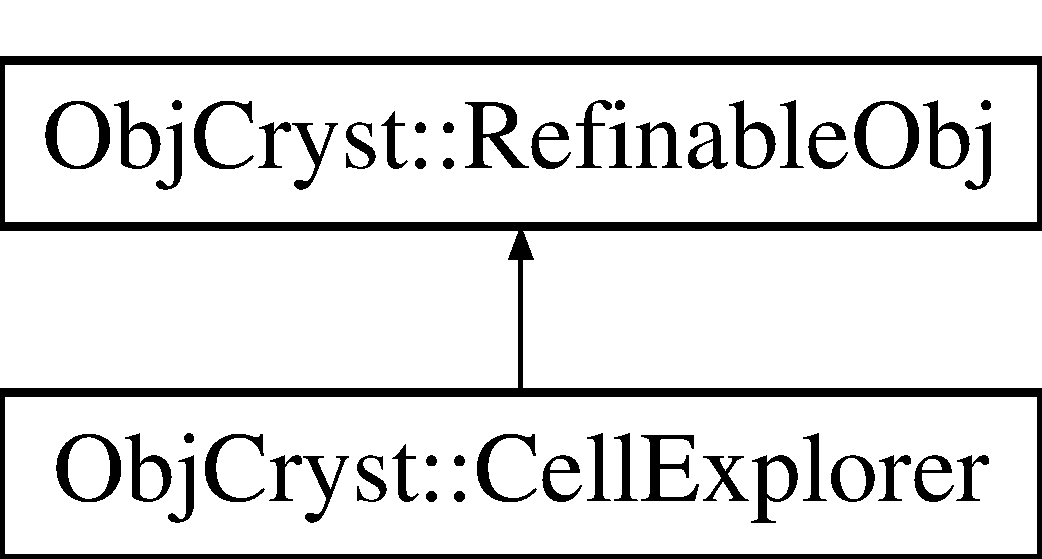
\includegraphics[height=3.000000cm]{a00014}
\end{center}
\end{figure}
\subsubsection*{Public Member Functions}
\begin{DoxyCompactItemize}
\item 
{\bf Atom} ()
\begin{DoxyCompactList}\small\item\em Default constructor. \end{DoxyCompactList}\item 
{\bf Atom} (const R\-E\-A\-L x, const R\-E\-A\-L y, const R\-E\-A\-L z, const string \&name, const {\bf Scattering\-Power} $\ast$pow)
\begin{DoxyCompactList}\small\item\em \doxyref{Atom}{p.}{a00014} constructor. \end{DoxyCompactList}\item 
{\bf Atom} (const R\-E\-A\-L x, const R\-E\-A\-L y, const R\-E\-A\-L z, const string \&name, const {\bf Scattering\-Power} $\ast$pow, const R\-E\-A\-L popu)
\begin{DoxyCompactList}\small\item\em \doxyref{Atom}{p.}{a00014} constructor. \end{DoxyCompactList}\item 
{\bf Atom} (const {\bf Atom} \&old)\label{a00014_a4882db30ef33e70582b354db8e76a07c}

\begin{DoxyCompactList}\small\item\em Copy constructor. \end{DoxyCompactList}\item 
virtual {\bf Atom} $\ast$ {\bf Create\-Copy} () const 
\item 
{\bf $\sim$\-Atom} ()\label{a00014_a86039a28098c9b48e7f4f57636a7e55d}

\begin{DoxyCompactList}\small\item\em Destructor... \end{DoxyCompactList}\item 
virtual const string \& {\bf Get\-Class\-Name} () const 
\begin{DoxyCompactList}\small\item\em Name for this class (\char`\"{}\-Refinable\-Obj\char`\"{}, \char`\"{}\-Crystal\char`\"{},...). \end{DoxyCompactList}\item 
virtual void {\bfseries operator=} (const {\bf Atom} \&rhs)\label{a00014_afc87e2009e5a0ad02311ff072b4f3b3e}

\item 
void {\bf Init} (const R\-E\-A\-L x, const R\-E\-A\-L y, const R\-E\-A\-L z, const string \&name, const {\bf Scattering\-Power} $\ast$pow, const R\-E\-A\-L popu=1)
\begin{DoxyCompactList}\small\item\em initialize the atom (used for arrays of atoms). \end{DoxyCompactList}\item 
virtual int {\bf Get\-Nb\-Component} () const \label{a00014_a7739a016c88ab32355e67b1c03fe97f0}

\begin{DoxyCompactList}\small\item\em Number of components in the scatterer (eg number of point scatterers) \end{DoxyCompactList}\item 
virtual const \\*
{\bf Scattering\-Component\-List} \& {\bf Get\-Scattering\-Component\-List} () const 
\begin{DoxyCompactList}\small\item\em Get the list of all scattering components for this scatterer. \end{DoxyCompactList}\item 
virtual string {\bf Get\-Component\-Name} (const int i) const 
\begin{DoxyCompactList}\small\item\em Name for the i-\/th component of this scatterer. \end{DoxyCompactList}\item 
virtual void {\bf Print} () const \label{a00014_a6c6836c4aa9d1510d64c7916d6ad47e2}

\begin{DoxyCompactList}\small\item\em Print some info about the scatterer (ideally this should be one line...). \end{DoxyCompactList}\item 
R\-E\-A\-L {\bf Get\-Mass} () const 
\begin{DoxyCompactList}\small\item\em Returns the molar mass of the atom. \end{DoxyCompactList}\item 
R\-E\-A\-L {\bf Get\-Radius} () const 
\begin{DoxyCompactList}\small\item\em Returns the radius (in Angstroems) of the atom. \end{DoxyCompactList}\item 
virtual ostream \& {\bf P\-O\-V\-Ray\-Description} (ostream \&os, const {\bf Crystal\-P\-O\-V\-Ray\-Options} \&options) const 
\begin{DoxyCompactList}\small\item\em X\-M\-L\-Output a description of the scatterer for P\-O\-V\-Ray. \end{DoxyCompactList}\item 
virtual void {\bf G\-L\-Init\-Display\-List} (const bool only\-Independent\-Atoms=false, const R\-E\-A\-L x\-Min=-\/.\-1, const R\-E\-A\-L x\-Max=1.\-1, const R\-E\-A\-L y\-Min=-\/.\-1, const R\-E\-A\-L y\-Max=1.\-1, const R\-E\-A\-L z\-Min=-\/.\-1, const R\-E\-A\-L z\-Max=1.\-1, const bool display\-Enantiomer=false, const bool display\-Names=false) const 
\item 
bool {\bf Is\-Dummy} () const \label{a00014_a672b84cd14db777c2f449d52671a3b15}

\begin{DoxyCompactList}\small\item\em Is this a dummy atom ? (ie no \doxyref{Scattering\-Power}{p.}{a00096}) Dummy atoms should not exist ! \end{DoxyCompactList}\item 
virtual void {\bf X\-M\-L\-Output} (ostream \&os, int indent=0) const 
\begin{DoxyCompactList}\small\item\em Output to stream in well-\/formed X\-M\-L. \end{DoxyCompactList}\item 
virtual void {\bf X\-M\-L\-Input} (istream \&is, const {\bf X\-M\-L\-Cryst\-Tag} \&tag)
\begin{DoxyCompactList}\small\item\em Input From stream. \end{DoxyCompactList}\item 
const {\bf Scattering\-Power} \& {\bf Get\-Scattering\-Power} () const \label{a00014_a63893a902cb731f552cb573c58ec94bb}

\begin{DoxyCompactList}\small\item\em Get the \doxyref{Scattering\-Power\-Atom}{p.}{a00097} corresponding to this atom. \end{DoxyCompactList}\item 
virtual void {\bf Get\-Gene\-Group} (const {\bf Refinable\-Obj} \&obj, Cryst\-Vector\-\_\-uint \&group\-Index, unsigned int \&first\-Group) const 
\begin{DoxyCompactList}\small\item\em Get the gene group assigned to each parameter. \end{DoxyCompactList}\end{DoxyCompactItemize}
\subsubsection*{Private Member Functions}
\begin{DoxyCompactItemize}
\item 
virtual void {\bf Init\-Ref\-Par\-List} ()\label{a00014_a72fe4868d70c8068483ba635029bbc86}

\begin{DoxyCompactList}\small\item\em Prepare refinable parameters for the scatterer object. \end{DoxyCompactList}\end{DoxyCompactItemize}
\subsubsection*{Private Attributes}
\begin{DoxyCompactItemize}
\item 
{\bf Scattering\-Component\-List} {\bf m\-Scatt\-Comp\-List}\label{a00014_aa9fc76a4412ca0726a478612caf02ead}

\begin{DoxyCompactList}\small\item\em The list of scattering components. \end{DoxyCompactList}\item 
const {\bf Scattering\-Power} $\ast$ {\bf mp\-Scatt\-Pow\-Atom}\label{a00014_a2ca524de2384b4beb111db9ed789f9fc}

\begin{DoxyCompactList}\small\item\em The \doxyref{Scattering\-Power\-Atom}{p.}{a00097} associated to that atom. \end{DoxyCompactList}\end{DoxyCompactItemize}
\subsubsection*{Additional Inherited Members}


\subsubsection{Detailed Description}
The basic atom scatterer, in a crystal. 

This class records the position of the atom, and has a pointer to its \doxyref{Scattering\-Power\-Atom}{p.}{a00097}.

\begin{DoxyNote}{Note}
there can be 'Dummy' atoms, for which the used symbol is \char`\"{}\-X\char`\"{}, and which have no scattering power (use with caution\-: dummy atoms are only supposed to be used within \doxyref{Z\-Scatterer}{p.}{a00162}) 
\end{DoxyNote}


\subsubsection{Constructor \& Destructor Documentation}
\index{Obj\-Cryst\-::\-Atom@{Obj\-Cryst\-::\-Atom}!Atom@{Atom}}
\index{Atom@{Atom}!ObjCryst::Atom@{Obj\-Cryst\-::\-Atom}}
\paragraph[{Atom}]{\setlength{\rightskip}{0pt plus 5cm}Obj\-Cryst\-::\-Atom\-::\-Atom (
\begin{DoxyParamCaption}
{}
\end{DoxyParamCaption}
)}\label{a00014_afa78c541a05f1210e9913c4591752042}


Default constructor. 

The \doxyref{Atom}{p.}{a00014} {\itshape must} be initialized thereafter using \doxyref{Atom\-::\-Init()}{p.}{a00014_ab05ef76113333041255789dba4bb60cd} \index{Obj\-Cryst\-::\-Atom@{Obj\-Cryst\-::\-Atom}!Atom@{Atom}}
\index{Atom@{Atom}!ObjCryst::Atom@{Obj\-Cryst\-::\-Atom}}
\paragraph[{Atom}]{\setlength{\rightskip}{0pt plus 5cm}Obj\-Cryst\-::\-Atom\-::\-Atom (
\begin{DoxyParamCaption}
\item[{const R\-E\-A\-L}]{x, }
\item[{const R\-E\-A\-L}]{y, }
\item[{const R\-E\-A\-L}]{z, }
\item[{const string \&}]{name, }
\item[{const {\bf Scattering\-Power} $\ast$}]{pow}
\end{DoxyParamCaption}
)}\label{a00014_a8f37e515c9e847ba20cc1033cd54e7b8}


\doxyref{Atom}{p.}{a00014} constructor. 


\begin{DoxyParams}{Parameters}
{\em x,y,z} & \-: {\itshape fractional} coordinates of the atom \\
\hline
{\em pow} & \-: the \doxyref{Scattering\-Power}{p.}{a00096} associated to this atom. Must be allocated separately. \\
\hline
{\em name} & \-: name of the atom ('Ta1','Sm2', 'Tungsten\-\_\-1'...). The name can have {\itshape any} format but spaces should be avoided. \\
\hline
\end{DoxyParams}
\index{Obj\-Cryst\-::\-Atom@{Obj\-Cryst\-::\-Atom}!Atom@{Atom}}
\index{Atom@{Atom}!ObjCryst::Atom@{Obj\-Cryst\-::\-Atom}}
\paragraph[{Atom}]{\setlength{\rightskip}{0pt plus 5cm}Obj\-Cryst\-::\-Atom\-::\-Atom (
\begin{DoxyParamCaption}
\item[{const R\-E\-A\-L}]{x, }
\item[{const R\-E\-A\-L}]{y, }
\item[{const R\-E\-A\-L}]{z, }
\item[{const string \&}]{name, }
\item[{const {\bf Scattering\-Power} $\ast$}]{pow, }
\item[{const R\-E\-A\-L}]{popu}
\end{DoxyParamCaption}
)}\label{a00014_a1a4253d4b5ea4d8777963a43c7817e87}


\doxyref{Atom}{p.}{a00014} constructor. 


\begin{DoxyParams}{Parameters}
{\em x,y,z} & \-: {\itshape fractional} coordinates of the atom \\
\hline
{\em popu} & \-: the population of the atom (0.\-0-\/$>$1.\-0) This should take into account the multiplicity of the atom. For an atom in group P2 and on the 2 axis, this should be set to 0.\-5, {\bfseries unless} you are using the dynamical occupancy correction (recommended for global optimizations). See \doxyref{Crystal\-::\-Calc\-Dyn\-Pop\-Corr()}{p.}{a00026_a69975008974c9603ebb794bb6bb20fe8} and \doxyref{Crystal\-::m\-Use\-Dyn\-Pop\-Corr}{p.}{a00026_aa75ade2fea9a50b3e6fb08773f607a13}\\
\hline
{\em pow} & \-: the \doxyref{Scattering\-Power}{p.}{a00096} associated to this atom. Must be allocated separatly. \\
\hline
{\em name} & \-: name of the atom ('Ta1','Sm2', 'Tungsten\-\_\-1'...). The name can have {\itshape any} format but spaces should be avoided (just a precaution) \\
\hline
\end{DoxyParams}


\subsubsection{Member Function Documentation}
\index{Obj\-Cryst\-::\-Atom@{Obj\-Cryst\-::\-Atom}!Create\-Copy@{Create\-Copy}}
\index{Create\-Copy@{Create\-Copy}!ObjCryst::Atom@{Obj\-Cryst\-::\-Atom}}
\paragraph[{Create\-Copy}]{\setlength{\rightskip}{0pt plus 5cm}virtual {\bf Atom}$\ast$ Obj\-Cryst\-::\-Atom\-::\-Create\-Copy (
\begin{DoxyParamCaption}
{}
\end{DoxyParamCaption}
) const\hspace{0.3cm}{\ttfamily [virtual]}}\label{a00014_af5215404ae1f180ed84046700845f92a}
so-\/called Virtual copy constructor, needed to make copies of arrays of Scatterers 

Implements {\bf Obj\-Cryst\-::\-Scatterer} \doxyref{}{p.}{a00091_a4d374adcff97163a24492d362f6def73}.

\index{Obj\-Cryst\-::\-Atom@{Obj\-Cryst\-::\-Atom}!Get\-Class\-Name@{Get\-Class\-Name}}
\index{Get\-Class\-Name@{Get\-Class\-Name}!ObjCryst::Atom@{Obj\-Cryst\-::\-Atom}}
\paragraph[{Get\-Class\-Name}]{\setlength{\rightskip}{0pt plus 5cm}virtual const string\& Obj\-Cryst\-::\-Atom\-::\-Get\-Class\-Name (
\begin{DoxyParamCaption}
{}
\end{DoxyParamCaption}
) const\hspace{0.3cm}{\ttfamily [virtual]}}\label{a00014_a9f0d1cb7c3b1db1baf84076e5da0ca0e}


Name for this class (\char`\"{}\-Refinable\-Obj\char`\"{}, \char`\"{}\-Crystal\char`\"{},...). 

This is only useful to distinguish different classes when picking up objects from the \doxyref{Refinable\-Obj}{p.}{a00077} Global Registry 

Reimplemented from {\bf Obj\-Cryst\-::\-Scatterer} \doxyref{}{p.}{a00091_a374fc1bb2887ab1f61d456326d97c05f}.

\index{Obj\-Cryst\-::\-Atom@{Obj\-Cryst\-::\-Atom}!Get\-Component\-Name@{Get\-Component\-Name}}
\index{Get\-Component\-Name@{Get\-Component\-Name}!ObjCryst::Atom@{Obj\-Cryst\-::\-Atom}}
\paragraph[{Get\-Component\-Name}]{\setlength{\rightskip}{0pt plus 5cm}virtual string Obj\-Cryst\-::\-Atom\-::\-Get\-Component\-Name (
\begin{DoxyParamCaption}
\item[{const int}]{i}
\end{DoxyParamCaption}
) const\hspace{0.3cm}{\ttfamily [virtual]}}\label{a00014_a88fed92945210af0e6cf28e34fa545f4}


Name for the i-\/th component of this scatterer. 

If the component is an \doxyref{Atom}{p.}{a00014}, Then the name is that of the atom. Else, it is the name of the scatterer plus the component number in the scatterer plus the name of the \doxyref{Scattering\-Power}{p.}{a00096}. \begin{DoxyNote}{Note}
It would be better to return a reference, but we don't want to keep a name for all components... Weeelll, needs some more thinking... see what performance hit results (if any).
\end{DoxyNote}
\begin{DoxyRefDesc}{Bug}
\item[{\bf Bug}]does not take into account dummy atoms !! \end{DoxyRefDesc}


Implements {\bf Obj\-Cryst\-::\-Scatterer} \doxyref{}{p.}{a00091_a42bdf508da6a90859a5a61e16c27d47e}.

\index{Obj\-Cryst\-::\-Atom@{Obj\-Cryst\-::\-Atom}!Get\-Gene\-Group@{Get\-Gene\-Group}}
\index{Get\-Gene\-Group@{Get\-Gene\-Group}!ObjCryst::Atom@{Obj\-Cryst\-::\-Atom}}
\paragraph[{Get\-Gene\-Group}]{\setlength{\rightskip}{0pt plus 5cm}virtual void Obj\-Cryst\-::\-Atom\-::\-Get\-Gene\-Group (
\begin{DoxyParamCaption}
\item[{const {\bf Refinable\-Obj} \&}]{obj, }
\item[{Cryst\-Vector\-\_\-uint \&}]{group\-Index, }
\item[{unsigned int \&}]{first\-Group}
\end{DoxyParamCaption}
) const\hspace{0.3cm}{\ttfamily [virtual]}}\label{a00014_a01645142310cf68d21b50ec514a0af77}


Get the gene group assigned to each parameter. 

Each parameter (a {\itshape gene} in terms of genetic algorithms) can be assigned to a gene group. Thus when mating two configurations, genes will be exchanged by groups. By default (in the base Refinabe\-Obj class), each parameter is alone in its group. Derived classes can group genes for a better s$\ast$$\ast$ life.

The number identifying a gene group only has a meaning in a given object. It can also change on subsequent calls, and thus is not unique.


\begin{DoxyParams}{Parameters}
{\em obj} & the , supplied by an algorithm class (\doxyref{Optimization\-Obj}{p.}{a00061},..), which contains a list of parameters, some of which (but possibly all or none) are parameters belonging to this object. \\
\hline
{\em group\-Index} & a vector of unsigned integers, one for each parameter in the input object, giving an unsigned integer value as gene group index. At the beginning this vector should contain only zeros (no group assigned). \\
\hline
{\em first\-Group} & this is the number of groups which have already been assigned, plus one. The gene groups returned by this object will start from this value, and increment {\bfseries first\-Group} for each gene group used, so that different \doxyref{Refinable\-Obj}{p.}{a00077} cannot share a gene group. \\
\hline
\end{DoxyParams}
\begin{DoxyNote}{Note}
this function is not optimized, and should only be called at the beginning of a refinement. 
\end{DoxyNote}


Reimplemented from {\bf Obj\-Cryst\-::\-Refinable\-Obj} \doxyref{}{p.}{a00077_ad59c8ad2b0d7ee59fa3f399a54f05e54}.

\index{Obj\-Cryst\-::\-Atom@{Obj\-Cryst\-::\-Atom}!Get\-Mass@{Get\-Mass}}
\index{Get\-Mass@{Get\-Mass}!ObjCryst::Atom@{Obj\-Cryst\-::\-Atom}}
\paragraph[{Get\-Mass}]{\setlength{\rightskip}{0pt plus 5cm}R\-E\-A\-L Obj\-Cryst\-::\-Atom\-::\-Get\-Mass (
\begin{DoxyParamCaption}
{}
\end{DoxyParamCaption}
) const}\label{a00014_afbdf315ca2363179e5227fe47d7f9106}


Returns the molar mass of the atom. 

Values are extracted from the 'atominfo' package, which uses data from the C\-R\-C Handbook of Chemistry \& Physics, 63rd \& 70th editions The Mass is actually extracted from the \doxyref{Scattering\-Power\-Atom}{p.}{a00097}. \index{Obj\-Cryst\-::\-Atom@{Obj\-Cryst\-::\-Atom}!Get\-Radius@{Get\-Radius}}
\index{Get\-Radius@{Get\-Radius}!ObjCryst::Atom@{Obj\-Cryst\-::\-Atom}}
\paragraph[{Get\-Radius}]{\setlength{\rightskip}{0pt plus 5cm}R\-E\-A\-L Obj\-Cryst\-::\-Atom\-::\-Get\-Radius (
\begin{DoxyParamCaption}
{}
\end{DoxyParamCaption}
) const}\label{a00014_ac0e9f074ecf5a20cf73752d38d7cc453}


Returns the radius (in Angstroems) of the atom. 

Values are extracted from the 'atominfo' package, which uses data from the I\-C\-S\-D/\-C\-R\-Y\-S\-T\-I\-N Manual The Radius is extracted from the \doxyref{Scattering\-Power\-Atom}{p.}{a00097}. \index{Obj\-Cryst\-::\-Atom@{Obj\-Cryst\-::\-Atom}!Get\-Scattering\-Component\-List@{Get\-Scattering\-Component\-List}}
\index{Get\-Scattering\-Component\-List@{Get\-Scattering\-Component\-List}!ObjCryst::Atom@{Obj\-Cryst\-::\-Atom}}
\paragraph[{Get\-Scattering\-Component\-List}]{\setlength{\rightskip}{0pt plus 5cm}virtual const {\bf Scattering\-Component\-List}\& Obj\-Cryst\-::\-Atom\-::\-Get\-Scattering\-Component\-List (
\begin{DoxyParamCaption}
{}
\end{DoxyParamCaption}
) const\hspace{0.3cm}{\ttfamily [virtual]}}\label{a00014_a3483660b1d08b113af61d708ecff8d1a}


Get the list of all scattering components for this scatterer. 

This is the most important function of this class, giving the list of scattering positions along with the associated \doxyref{Scattering\-Power}{p.}{a00096}. 

Implements {\bf Obj\-Cryst\-::\-Scatterer} \doxyref{}{p.}{a00091_aca0e08e3793cc69d31fce53e481c2a67}.

\index{Obj\-Cryst\-::\-Atom@{Obj\-Cryst\-::\-Atom}!G\-L\-Init\-Display\-List@{G\-L\-Init\-Display\-List}}
\index{G\-L\-Init\-Display\-List@{G\-L\-Init\-Display\-List}!ObjCryst::Atom@{Obj\-Cryst\-::\-Atom}}
\paragraph[{G\-L\-Init\-Display\-List}]{\setlength{\rightskip}{0pt plus 5cm}virtual void Obj\-Cryst\-::\-Atom\-::\-G\-L\-Init\-Display\-List (
\begin{DoxyParamCaption}
\item[{const bool}]{no\-Symmetrics = {\ttfamily false}, }
\item[{const R\-E\-A\-L}]{x\-Min = {\ttfamily -\/.1}, }
\item[{const R\-E\-A\-L}]{x\-Max = {\ttfamily 1.1}, }
\item[{const R\-E\-A\-L}]{y\-Min = {\ttfamily -\/.1}, }
\item[{const R\-E\-A\-L}]{y\-Max = {\ttfamily 1.1}, }
\item[{const R\-E\-A\-L}]{z\-Min = {\ttfamily -\/.1}, }
\item[{const R\-E\-A\-L}]{z\-Max = {\ttfamily 1.1}, }
\item[{const bool}]{display\-Enantiomer = {\ttfamily false}, }
\item[{const bool}]{display\-Names = {\ttfamily false}}
\end{DoxyParamCaption}
) const\hspace{0.3cm}{\ttfamily [virtual]}}\label{a00014_a14e239415f6923d83ceff1347b89393b}
Create an Open\-G\-L Display List of the scatterer. This should only be called by a \doxyref{Crystal}{p.}{a00026} object.


\begin{DoxyParams}{Parameters}
{\em no\-Symmetrics} & if false (the default), then all symmetrics are shown in the 3\-D display, within the limits defined by the min/max parameters \textbackslash{} param x\-Min,x\-Max,y\-Min,y\-Max,z\-Min,z\-Max\-: in fractionnal coordinates, the region in which we want scaterrer to be displayed. The test is made on the center of the scatterer (eg a \doxyref{Z\-Scatterer}{p.}{a00162} (molecule) will not be 'cut' on the border). \\
\hline
{\em display\-Names} & if true, only the names of the scatterers will be displayed, at the position of the scatterers (to actually see them, they will have to be translated with respect to the drawing of the scatterers). \\
\hline
\end{DoxyParams}


Implements {\bf Obj\-Cryst\-::\-Scatterer} \doxyref{}{p.}{a00091_a4eaf9cf9780bef83e40155810db120a0}.

\index{Obj\-Cryst\-::\-Atom@{Obj\-Cryst\-::\-Atom}!Init@{Init}}
\index{Init@{Init}!ObjCryst::Atom@{Obj\-Cryst\-::\-Atom}}
\paragraph[{Init}]{\setlength{\rightskip}{0pt plus 5cm}void Obj\-Cryst\-::\-Atom\-::\-Init (
\begin{DoxyParamCaption}
\item[{const R\-E\-A\-L}]{x, }
\item[{const R\-E\-A\-L}]{y, }
\item[{const R\-E\-A\-L}]{z, }
\item[{const string \&}]{name, }
\item[{const {\bf Scattering\-Power} $\ast$}]{pow, }
\item[{const R\-E\-A\-L}]{popu = {\ttfamily 1}}
\end{DoxyParamCaption}
)}\label{a00014_ab05ef76113333041255789dba4bb60cd}


initialize the atom (used for arrays of atoms). 


\begin{DoxyParams}{Parameters}
{\em x,y,z} & \-: {\itshape fractional} coordinates of the atom \\
\hline
{\em pow} & \-: the \doxyref{Scattering\-Power}{p.}{a00096} associated to this atom. Must be allocated separately. \\
\hline
{\em name} & \-: name of the atom ('Ta1','Sm2', 'Tungsten\-\_\-1'...). \\
\hline
\end{DoxyParams}
\index{Obj\-Cryst\-::\-Atom@{Obj\-Cryst\-::\-Atom}!P\-O\-V\-Ray\-Description@{P\-O\-V\-Ray\-Description}}
\index{P\-O\-V\-Ray\-Description@{P\-O\-V\-Ray\-Description}!ObjCryst::Atom@{Obj\-Cryst\-::\-Atom}}
\paragraph[{P\-O\-V\-Ray\-Description}]{\setlength{\rightskip}{0pt plus 5cm}virtual ostream\& Obj\-Cryst\-::\-Atom\-::\-P\-O\-V\-Ray\-Description (
\begin{DoxyParamCaption}
\item[{ostream \&}]{os, }
\item[{const {\bf Crystal\-P\-O\-V\-Ray\-Options} \&}]{options}
\end{DoxyParamCaption}
) const\hspace{0.3cm}{\ttfamily [virtual]}}\label{a00014_a2994321bc2974d853f36b011d23a94b3}


X\-M\-L\-Output a description of the scatterer for P\-O\-V\-Ray. 



Implements {\bf Obj\-Cryst\-::\-Scatterer} \doxyref{}{p.}{a00091_a708cc857f82c9af4cbdf4d9334449d0f}.

\index{Obj\-Cryst\-::\-Atom@{Obj\-Cryst\-::\-Atom}!X\-M\-L\-Input@{X\-M\-L\-Input}}
\index{X\-M\-L\-Input@{X\-M\-L\-Input}!ObjCryst::Atom@{Obj\-Cryst\-::\-Atom}}
\paragraph[{X\-M\-L\-Input}]{\setlength{\rightskip}{0pt plus 5cm}virtual void Obj\-Cryst\-::\-Atom\-::\-X\-M\-L\-Input (
\begin{DoxyParamCaption}
\item[{istream \&}]{is, }
\item[{const {\bf X\-M\-L\-Cryst\-Tag} \&}]{tag}
\end{DoxyParamCaption}
)\hspace{0.3cm}{\ttfamily [virtual]}}\label{a00014_a08fe773b05dd0dc748b8008636b56187}


Input From stream. 

\begin{DoxyRefDesc}{Todo}
\item[{\bf Todo}]Add an bool X\-M\-L\-Input\-Tag(is,tag) function to recognize all the tags from the stream. So that each inherited class can use the X\-M\-L\-Input\-Tag function from its parent (ie take advantage of inheritance). The children class would first try to interpret the tag, then if unsuccessful would pass it to its parent (thus allowing overloading), etc... \end{DoxyRefDesc}


Reimplemented from {\bf Obj\-Cryst\-::\-Refinable\-Obj} \doxyref{}{p.}{a00077_ac13a4045c3f187879443c8615c38d623}.

\index{Obj\-Cryst\-::\-Atom@{Obj\-Cryst\-::\-Atom}!X\-M\-L\-Output@{X\-M\-L\-Output}}
\index{X\-M\-L\-Output@{X\-M\-L\-Output}!ObjCryst::Atom@{Obj\-Cryst\-::\-Atom}}
\paragraph[{X\-M\-L\-Output}]{\setlength{\rightskip}{0pt plus 5cm}virtual void Obj\-Cryst\-::\-Atom\-::\-X\-M\-L\-Output (
\begin{DoxyParamCaption}
\item[{ostream \&}]{os, }
\item[{int}]{indent = {\ttfamily 0}}
\end{DoxyParamCaption}
) const\hspace{0.3cm}{\ttfamily [virtual]}}\label{a00014_a83bd4047affa8c4de3126465595b77cb}


Output to stream in well-\/formed X\-M\-L. 

\begin{DoxyRefDesc}{Todo}
\item[{\bf Todo}]Use inheritance.. as for X\-M\-L\-Input\-Tag()... \end{DoxyRefDesc}


Reimplemented from {\bf Obj\-Cryst\-::\-Refinable\-Obj} \doxyref{}{p.}{a00077_a7b9b6ed0f8dcf753d398c35e073de973}.



The documentation for this class was generated from the following file\-:\begin{DoxyCompactItemize}
\item 
Atom.\-h\end{DoxyCompactItemize}

\subsection{Chronometer Class Reference}
\label{a00015}\index{Chronometer@{Chronometer}}


Simple chronometer class, with microsecond precision.  


\subsubsection*{Public Member Functions}
\begin{DoxyCompactItemize}
\item 
void {\bfseries start} ()\label{a00015_aef429cdb6aae70bf6a8b540e426efb96}

\item 
void {\bfseries pause} ()\label{a00015_a5ec9df9b8c17e695bc5cce5607df0380}

\item 
void {\bfseries resume} ()\label{a00015_ac98118472c0cc0691d9891e1173f86a9}

\item 
void {\bfseries print} ()\label{a00015_a249f804f5f815299ecdb999fb3b10229}

\item 
float {\bfseries seconds} ()\label{a00015_aec1d1b7317d9ad05e923b65855b6a49b}

\end{DoxyCompactItemize}
\subsubsection*{Private Attributes}
\begin{DoxyCompactItemize}
\item 
bool {\bfseries m\-Paused}\label{a00015_a690e9d4287d4780546da0199f16b92ac}

\item 
boost\-::posix\-\_\-time\-::ptime {\bfseries m\-Time0}\label{a00015_ad9d1b8f615bfac6a1133202047fe3d48}

\item 
boost\-::posix\-\_\-time\-::ptime {\bfseries m\-Time1}\label{a00015_a1f74a906486b1a1d3d69519a41d9e33c}

\end{DoxyCompactItemize}


\subsubsection{Detailed Description}
Simple chronometer class, with microsecond precision. 

Reported time correspond to {\itshape real} time, i.\-e. not the time the program has been running independently from other programs. 

The documentation for this class was generated from the following file\-:\begin{DoxyCompactItemize}
\item 
Chronometer.\-h\end{DoxyCompactItemize}

\subsection{ci\_\-char\_\-traits Struct Reference}
\label{a00016}\index{ci\_\-char\_\-traits@{ci\_\-char\_\-traits}}


Case-\/insensitive string class From: Guru of the Week \#29 e.g.  
\subsubsection*{Static Public Member Functions}
\begin{DoxyCompactItemize}
\item 
static bool {\bfseries eq} (char c1, char c2)\label{a00016_ab7affd067081a44149cbdb5ddbd6388a}

\item 
static bool {\bfseries ne} (char c1, char c2)\label{a00016_a37eaee352a01e9557c164f58c7d0ae36}

\item 
static bool {\bfseries lt} (char c1, char c2)\label{a00016_a2658e35e7ccccd43faea5922aeea2855}

\item 
static int {\bfseries compare} (const char $\ast$s1, const char $\ast$s2, size\_\-t n)\label{a00016_aee3f3e6230d9e98ed5a820bb7d05c443}

\item 
static const char $\ast$ {\bfseries find} (const char $\ast$s, int n, char a)\label{a00016_a5968fc0112d4a24e2fa74da3700357b1}

\end{DoxyCompactItemize}


\subsubsection{Detailed Description}
Case-\/insensitive string class From: Guru of the Week \#29 e.g. : {\tt http://gcc.gnu.org/onlinedocs/libstdc++/21\_\-strings/gotw29a.txt}

Public domain. 

The documentation for this struct was generated from the following file:\begin{DoxyCompactItemize}
\item 
ci\_\-string.h\end{DoxyCompactItemize}

\subsection{Obj\-Cryst\-:\-:W\-X\-Molecule\-:\-:Cell\-Atom Struct Reference}
\label{a00017}\index{Obj\-Cryst\-::\-W\-X\-Molecule\-::\-Cell\-Atom@{Obj\-Cryst\-::\-W\-X\-Molecule\-::\-Cell\-Atom}}


Structure to store the \doxyref{Atom}{p.}{a00015} parameters.  


\subsubsection*{Public Attributes}
\begin{DoxyCompactItemize}
\item 
{\bf Mol\-Atom} $\ast$ {\bfseries mp\-Atom}\label{a00017_ad42e078ccf1193f1bda7394a07be31d5}

\item 
std\-::string {\bfseries m\-Name}\label{a00017_a6d1f3559b25ffb17b9095dd92b680e51}

\item 
const {\bf Scattering\-Power} $\ast$ {\bfseries mp\-Scattering\-Power}\label{a00017_a543efd9bcc607f7ca87ae672bb3ab858}

\item 
R\-E\-A\-L {\bfseries m\-X}\label{a00017_a78d75f4d42aa474bc6bcf6597bfa999d}

\item 
R\-E\-A\-L {\bfseries m\-Y}\label{a00017_a744ed5e33a9d2ec36243fc6c5a8c0caf}

\item 
R\-E\-A\-L {\bfseries m\-Z}\label{a00017_aed30b328634831e4c62971133f6be407}

\item 
bool {\bf m\-Need\-Update\-U\-I}\label{a00017_ae4923e30e4b7b2a22e2b74b0ac1b6c00}

\begin{DoxyCompactList}\small\item\em True if we need to update the displayed values. \end{DoxyCompactList}\end{DoxyCompactItemize}


\subsubsection{Detailed Description}
Structure to store the \doxyref{Atom}{p.}{a00015} parameters. 

The documentation for this struct was generated from the following file\-:\begin{DoxyCompactItemize}
\item 
wx\-Molecule.\-h\end{DoxyCompactItemize}

\subsection{Obj\-Cryst\-:\-:C\-I\-F\-Data\-:\-:C\-I\-F\-Atom Struct Reference}
\label{a00018}\index{Obj\-Cryst\-::\-C\-I\-F\-Data\-::\-C\-I\-F\-Atom@{Obj\-Cryst\-::\-C\-I\-F\-Data\-::\-C\-I\-F\-Atom}}


\doxyref{Atom}{p.}{a00008} record.  


\subsubsection*{Public Attributes}
\begin{DoxyCompactItemize}
\item 
std\-::string {\bf m\-Label}\label{a00018_a32f3b29fdecc1ea4ed42fd2f588f7dc2}

\begin{DoxyCompactList}\small\item\em Label of the atom, or empty string (\-\_\-atom\-\_\-site\-\_\-label). \end{DoxyCompactList}\item 
std\-::string {\bf m\-Symbol}\label{a00018_a70e19874d95cb054f2e6b4da29716708}

\begin{DoxyCompactList}\small\item\em Symbol of the atom, or empty string (\-\_\-atom\-\_\-type\-\_\-symbol or \-\_\-atom\-\_\-site\-\_\-type\-\_\-symbol). \end{DoxyCompactList}\item 
std\-::vector$<$ float $>$ {\bf m\-Coord\-Frac}\label{a00018_a0fb94664112092c339319ac149bf8410}

\begin{DoxyCompactList}\small\item\em Fractionnal coordinates ({\itshape atom\-\_\-site\-\_\-fract}\{x,y,z\}) or empty vector. \end{DoxyCompactList}\item 
std\-::vector$<$ float $>$ {\bf m\-Coord\-Cart}
\begin{DoxyCompactList}\small\item\em Cartesian coordinates in Angstroem ({\itshape atom\-\_\-site\-\_\-\-Cartn}\{x,y,z\}) or empty vector. \end{DoxyCompactList}\item 
float {\bf m\-Occupancy}\label{a00018_a95523357bde2b4dc4779e2e1a0bebba5}

\begin{DoxyCompactList}\small\item\em Site occupancy, or -\/1. \end{DoxyCompactList}\end{DoxyCompactItemize}


\subsubsection{Detailed Description}
\doxyref{Atom}{p.}{a00008} record. 

\subsubsection{Member Data Documentation}
\index{Obj\-Cryst\-::\-C\-I\-F\-Data\-::\-C\-I\-F\-Atom@{Obj\-Cryst\-::\-C\-I\-F\-Data\-::\-C\-I\-F\-Atom}!m\-Coord\-Cart@{m\-Coord\-Cart}}
\index{m\-Coord\-Cart@{m\-Coord\-Cart}!ObjCryst::CIFData::CIFAtom@{Obj\-Cryst\-::\-C\-I\-F\-Data\-::\-C\-I\-F\-Atom}}
\paragraph[{m\-Coord\-Cart}]{\setlength{\rightskip}{0pt plus 5cm}std\-::vector$<$float$>$ Obj\-Cryst\-::\-C\-I\-F\-Data\-::\-C\-I\-F\-Atom\-::m\-Coord\-Cart}\label{a00018_a0d0447f70b4bfa0227733a1b3cf51727}


Cartesian coordinates in Angstroem ({\itshape atom\-\_\-site\-\_\-\-Cartn}\{x,y,z\}) or empty vector. 

Transformation to fractionnal coordinates currently assumes \char`\"{}a parallel to x; b in the plane of y and z\char`\"{} (see \-\_\-atom\-\_\-sites\-\_\-\-Cartn\-\_\-transform\-\_\-axes) 

The documentation for this struct was generated from the following file\-:\begin{DoxyCompactItemize}
\item 
C\-I\-F.\-h\end{DoxyCompactItemize}

\subsection{Obj\+Cryst\+:\+:W\+X\+Molecule\+:\+:Cell\+Dihedral\+Angle Struct Reference}
\label{a00019}\index{Obj\+Cryst\+::\+W\+X\+Molecule\+::\+Cell\+Dihedral\+Angle@{Obj\+Cryst\+::\+W\+X\+Molecule\+::\+Cell\+Dihedral\+Angle}}


Structure to store the dihedral angles current values.  


\subsubsection*{Public Attributes}
\begin{DoxyCompactItemize}
\item 
{\bf Mol\+Dihedral\+Angle} $\ast$ {\bfseries mp\+Dihedral\+Angle}\label{a00019_a71b64f0d32c3be8ee6eddcb541b8ff3a}

\item 
std\+::string {\bfseries m\+Atom1}\label{a00019_a5017846593e27be16059f9d64c8def16}

\item 
std\+::string {\bfseries m\+Atom2}\label{a00019_ab7d5eccf2380f164c09f151e0d018453}

\item 
std\+::string {\bfseries m\+Atom3}\label{a00019_a43a40794a36bdd7170c28f76a99d2ee9}

\item 
std\+::string {\bfseries m\+Atom4}\label{a00019_aa82b25fba5aa8f0a70e216ee601f18a1}

\item 
R\+E\+A\+L {\bfseries m\+Angle}\label{a00019_a227fe316e99f5b57202687f76b5367ec}

\item 
R\+E\+A\+L {\bfseries m\+Angle0}\label{a00019_ab422002f0ffd7af2deb566be02a6ba6c}

\item 
R\+E\+A\+L {\bfseries m\+Sigma}\label{a00019_aea437e0e56b9ae0fa2f3ade2491c5513}

\item 
R\+E\+A\+L {\bfseries m\+Delta}\label{a00019_a7ce376d1b84e19557012de335e2b29b5}

\item 
bool {\bf m\+Need\+Update\+U\+I}\label{a00019_a635d878acce3c594ca0225d7e58a4119}

\begin{DoxyCompactList}\small\item\em True if we need to update the displayed values. \end{DoxyCompactList}\end{DoxyCompactItemize}


\subsubsection{Detailed Description}
Structure to store the dihedral angles current values. 

The documentation for this struct was generated from the following file\+:\begin{DoxyCompactItemize}
\item 
wx\+Molecule.\+h\end{DoxyCompactItemize}

\subsection{ObjCryst::Crystal Class Reference}
\label{a00020}\index{ObjCryst::Crystal@{ObjCryst::Crystal}}


\doxyref{Crystal}{p.}{a00020} class: Unit cell, spacegroup, scatterers.  
Inheritance diagram for ObjCryst::Crystal::\begin{figure}[H]
\begin{center}
\leavevmode
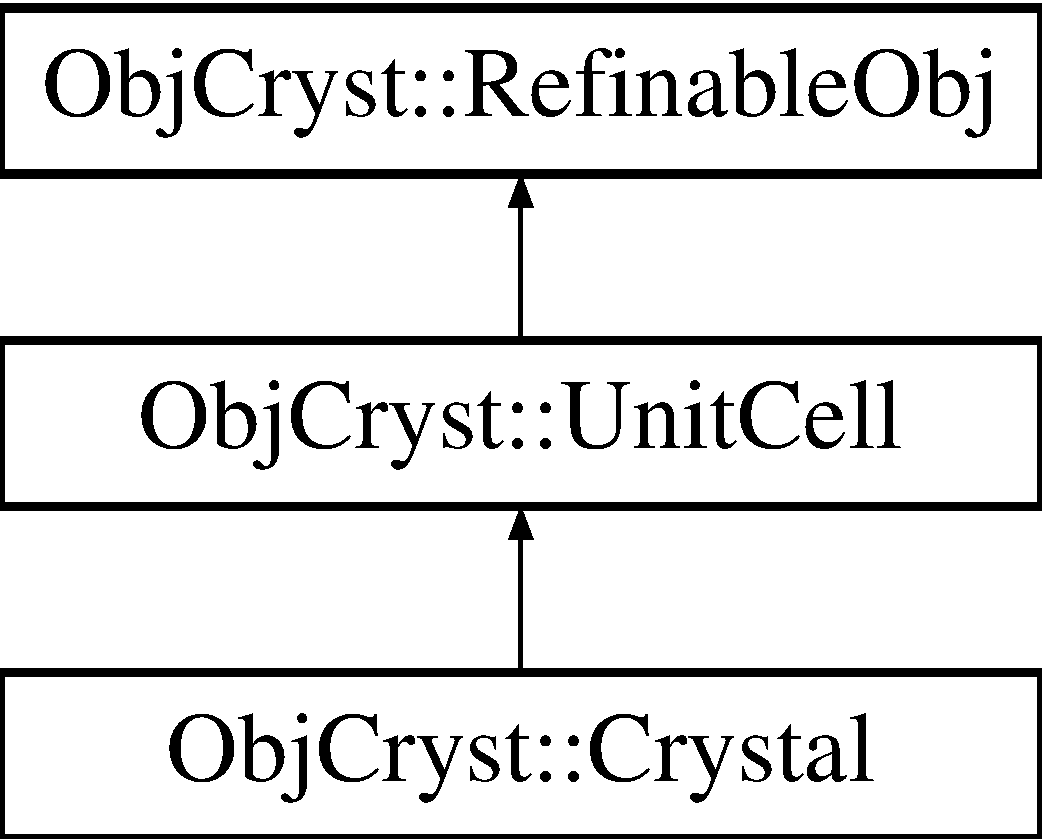
\includegraphics[height=3cm]{a00020}
\end{center}
\end{figure}
\subsubsection*{Classes}
\begin{DoxyCompactItemize}
\item 
struct {\bf BumpMergePar}
\begin{DoxyCompactList}\small\item\em Storage for anti-\/bump/merge parameters. \item\end{DoxyCompactList}\item 
struct {\bf Neighbour}
\begin{DoxyCompactList}\small\item\em Interatomic distance for a given neighbour. \item\end{DoxyCompactList}\item 
struct {\bf NeighbourHood}
\begin{DoxyCompactList}\small\item\em Table of neighbours for a given unique atom. \item\end{DoxyCompactList}\end{DoxyCompactItemize}
\subsubsection*{Public Types}
\begin{DoxyCompactItemize}
\item 
typedef std::map$<$ pair$<$ const {\bf ScatteringPower} $\ast$, const {\bf ScatteringPower} $\ast$ $>$, {\bf Crystal::BumpMergePar} $>$ {\bf VBumpMergePar}
\begin{DoxyCompactList}\small\item\em Anti-\/bump parameters. \item\end{DoxyCompactList}\end{DoxyCompactItemize}
\subsubsection*{Public Member Functions}
\begin{DoxyCompactItemize}
\item 
{\bf Crystal} ()\label{a00020_a4d9c152db2dfcea3c849d0a7ae547a2e}

\begin{DoxyCompactList}\small\item\em Default Constructor. \item\end{DoxyCompactList}\item 
{\bf Crystal} (const REAL a, const REAL b, const REAL c, const string \&SpaceGroupId)
\begin{DoxyCompactList}\small\item\em \doxyref{Crystal}{p.}{a00020} Constructor (orthorombic). \item\end{DoxyCompactList}\item 
{\bf Crystal} (const REAL a, const REAL b, const REAL c, const REAL alpha, const REAL beta, const REAL gamma, const string \&SpaceGroupId)
\begin{DoxyCompactList}\small\item\em \doxyref{Crystal}{p.}{a00020} Constructor (triclinic). \item\end{DoxyCompactList}\item 
{\bf Crystal} (const {\bf Crystal} \&oldCryst)\label{a00020_a4fd1bac8dbb8c119077f3b1f3d19153f}

\begin{DoxyCompactList}\small\item\em \doxyref{Crystal}{p.}{a00020} copy constructor. \item\end{DoxyCompactList}\item 
{\bf $\sim$Crystal} ()\label{a00020_a13a9e007a57aeb11a5d808099c56c2b5}

\begin{DoxyCompactList}\small\item\em \doxyref{Crystal}{p.}{a00020} destructor. \item\end{DoxyCompactList}\item 
virtual const string \& {\bf GetClassName} () const 
\begin{DoxyCompactList}\small\item\em Name for this class (\char`\"{}RefinableObj\char`\"{}, \char`\"{}Crystal\char`\"{},. \item\end{DoxyCompactList}\item 
void {\bf AddScatterer} ({\bf Scatterer} $\ast$scatt)
\begin{DoxyCompactList}\small\item\em Add a scatterer to the crystal. \item\end{DoxyCompactList}\item 
void {\bf RemoveScatterer} ({\bf Scatterer} $\ast$scatt, const bool del=true)\label{a00020_ac2755d27280cfa572aa334e6e596da98}

\begin{DoxyCompactList}\small\item\em Remove a \doxyref{Scatterer}{p.}{a00084}. This also deletes the scatterer unless del=false. \item\end{DoxyCompactList}\item 
long {\bf GetNbScatterer} () const \label{a00020_a5fb1f327104bd5cf5550265b1453a639}

\begin{DoxyCompactList}\small\item\em Number of scatterers in the crystal. \item\end{DoxyCompactList}\item 
{\bf Scatterer} \& {\bf GetScatt} (const string \&scattName)
\begin{DoxyCompactList}\small\item\em Provides an access to the scatterers. \item\end{DoxyCompactList}\item 
const {\bf Scatterer} \& {\bf GetScatt} (const string \&scattName) const 
\begin{DoxyCompactList}\small\item\em Provides a const access to the scatterers. \item\end{DoxyCompactList}\item 
{\bf Scatterer} \& {\bf GetScatt} (const long scattIndex)
\begin{DoxyCompactList}\small\item\em Provides an access to the scatterers. \item\end{DoxyCompactList}\item 
const {\bf Scatterer} \& {\bf GetScatt} (const long scattIndex) const 
\begin{DoxyCompactList}\small\item\em Provides a const access to the scatterers. \item\end{DoxyCompactList}\item 
{\bf ObjRegistry}$<$ {\bf Scatterer} $>$ \& {\bf GetScattererRegistry} ()\label{a00020_ad2e15e119a2cfc4104efd46672c63b64}

\begin{DoxyCompactList}\small\item\em Get the registry of scatterers. \item\end{DoxyCompactList}\item 
const {\bf ObjRegistry}$<$ {\bf Scatterer} $>$ \& {\bf GetScattererRegistry} () const \label{a00020_ac93eb73b0194e1550a0d6eb5b313ab44}

\begin{DoxyCompactList}\small\item\em Get the registry of scatterers. \item\end{DoxyCompactList}\item 
{\bf ObjRegistry}$<$ {\bf ScatteringPower} $>$ \& {\bf GetScatteringPowerRegistry} ()\label{a00020_a53d6f239dbfae0040c900e4d4e120e73}

\begin{DoxyCompactList}\small\item\em Get the registry of \doxyref{ScatteringPower}{p.}{a00089} included in this \doxyref{Crystal}{p.}{a00020}. \item\end{DoxyCompactList}\item 
const {\bf ObjRegistry}$<$ {\bf ScatteringPower} $>$ \& {\bf GetScatteringPowerRegistry} () const \label{a00020_abcc623c63dfe1085d28e7d73811fff16}

\begin{DoxyCompactList}\small\item\em Get the registry of \doxyref{ScatteringPower}{p.}{a00089} included in this \doxyref{Crystal}{p.}{a00020}. \item\end{DoxyCompactList}\item 
void {\bf AddScatteringPower} ({\bf ScatteringPower} $\ast$scattPow)
\begin{DoxyCompactList}\small\item\em Add a \doxyref{ScatteringPower}{p.}{a00089} for this \doxyref{Crystal}{p.}{a00020}. \item\end{DoxyCompactList}\item 
void {\bf RemoveScatteringPower} ({\bf ScatteringPower} $\ast$scattPow, const bool del=true)
\begin{DoxyCompactList}\small\item\em Remove a \doxyref{ScatteringPower}{p.}{a00089} for this \doxyref{Crystal}{p.}{a00020}. \item\end{DoxyCompactList}\item 
{\bf ScatteringPower} \& {\bf GetScatteringPower} (const string \&name)\label{a00020_a3a71094a078502bbb73f811f895cb438}

\begin{DoxyCompactList}\small\item\em Find a \doxyref{ScatteringPower}{p.}{a00089} from its name. Names must be unique in a given \doxyref{Crystal}{p.}{a00020}. \item\end{DoxyCompactList}\item 
const {\bf ScatteringPower} \& {\bf GetScatteringPower} (const string \&name) const \label{a00020_a5622a2ef63f40084527626c94085f90a}

\begin{DoxyCompactList}\small\item\em Find a \doxyref{ScatteringPower}{p.}{a00089} from its name. Names must be unique in a given \doxyref{Crystal}{p.}{a00020}. \item\end{DoxyCompactList}\item 
const {\bf RefinableObjClock} \& {\bf GetMasterClockScatteringPower} () const \label{a00020_a3b583a9655a174de9c21e139eea709dc}

\begin{DoxyCompactList}\small\item\em Get the clock which reports all changes in ScatteringPowers. \item\end{DoxyCompactList}\item 
virtual const {\bf ScatteringComponentList} \& {\bf GetScatteringComponentList} () const \label{a00020_a748d335480c372c5ef6cdf8716d9dd1a}

\begin{DoxyCompactList}\small\item\em Get the list of all scattering components. \item\end{DoxyCompactList}\item 
const {\bf RefinableObjClock} \& {\bf GetClockScattCompList} () const \label{a00020_a1deb673a7f01f6a71c659f28ddf5cd21}

\begin{DoxyCompactList}\small\item\em Get the list of all scattering components. \item\end{DoxyCompactList}\item 
void {\bf Print} (ostream \&os=cout) const 
\begin{DoxyCompactList}\small\item\em Prints some info about the crystal. \item\end{DoxyCompactList}\item 
CrystMatrix\_\-REAL {\bf GetMinDistanceTable} (const REAL minDistance=0.1) const 
\begin{DoxyCompactList}\small\item\em Minimum interatomic distance between all scattering components (atoms) in the crystal. \item\end{DoxyCompactList}\item 
void {\bf PrintMinDistanceTable} (const REAL minDistance=0.1, ostream \&os=cout) const 
\begin{DoxyCompactList}\small\item\em Print the minimum distance table between all scattering centers (atoms) in the crystal. \item\end{DoxyCompactList}\item 
ostream \& {\bf POVRayDescription} (ostream \&os, const {\bf CrystalPOVRayOptions} \&options) const 
\begin{DoxyCompactList}\small\item\em XMLOutput POV-\/Ray Description for this \doxyref{Crystal}{p.}{a00020}. \item\end{DoxyCompactList}\item 
virtual void {\bf GLInitDisplayList} (const bool onlyIndependentAtoms=false, const REAL xMin=-\/.1, const REAL xMax=1.1, const REAL yMin=-\/.1, const REAL yMax=1.1, const REAL zMin=-\/.1, const REAL zMax=1.1, const bool displayNames=false) const 
\begin{DoxyCompactList}\small\item\em Create an OpenGL DisplayList of the crystal. \item\end{DoxyCompactList}\item 
void {\bf CalcDynPopCorr} (const REAL overlapDist=1., const REAL mergeDist=.0) const 
\begin{DoxyCompactList}\small\item\em Compute the 'Dynamical population correction for all atoms. Atoms which are considered \char`\"{}equivalent\char`\"{} (ie currently with the same Z number) and which are overlapping see their Dynamical occupancy changed so that when they fully overlap, they are equivalent to 1 atom. \item\end{DoxyCompactList}\item 
void {\bf ResetDynPopCorr} () const \label{a00020_a9230b222fe2cde018c6b08fab6d5da8b}

\begin{DoxyCompactList}\small\item\em Reset Dynamical Population Correction factors (ie set it to 1). \item\end{DoxyCompactList}\item 
void {\bf SetUseDynPopCorr} (const int use)
\begin{DoxyCompactList}\small\item\em Set the use of dynamical population correction (\doxyref{Crystal::mUseDynPopCorr}{p.}{a00020_aa75ade2fea9a50b3e6fb08773f607a13}). \item\end{DoxyCompactList}\item 
REAL {\bf GetBumpMergeCost} () const 
\begin{DoxyCompactList}\small\item\em Get the Anti-\/bumping/pro-\/Merging cost function. \item\end{DoxyCompactList}\item 
void {\bf SetBumpMergeDistance} (const {\bf ScatteringPower} \&scatt1, const {\bf ScatteringPower} \&scatt2, const REAL dist=1.5)
\begin{DoxyCompactList}\small\item\em Set the Anti-\/bumping distance between two scattering types. \item\end{DoxyCompactList}\item 
void {\bf SetBumpMergeDistance} (const {\bf ScatteringPower} \&scatt1, const {\bf ScatteringPower} \&scatt2, const REAL dist, const bool allowMerge)\label{a00020_a74a095efbf1f414a0707532cb51f78ca}

\begin{DoxyCompactList}\small\item\em Set the Anti-\/bumping distance between two scattering types. \item\end{DoxyCompactList}\item 
void {\bf RemoveBumpMergeDistance} (const {\bf ScatteringPower} \&scatt1, const {\bf ScatteringPower} \&scatt2)\label{a00020_ac098ff50897a0afdec066d5f3872a5a1}

\begin{DoxyCompactList}\small\item\em Remove an Anti-\/bumping distance between two scattering types. \item\end{DoxyCompactList}\item 
const {\bf VBumpMergePar} \& {\bfseries GetBumpMergeParList} () const \label{a00020_a0e1cfe79846330b06619619a51af34d6}

\item 
{\bf VBumpMergePar} \& {\bfseries GetBumpMergeParList} ()\label{a00020_a454da6faa3699da08af3ed99f2193d9a}

\item 
const {\bf RefinableObjClock} \& {\bf GetClockScattererList} () const \label{a00020_a656dd25b9a62224144142fff3eba1627}

\begin{DoxyCompactList}\small\item\em When was the list of scatterers last changed ? \item\end{DoxyCompactList}\item 
virtual void {\bf XMLOutput} (ostream \&os, int indent=0) const 
\begin{DoxyCompactList}\small\item\em Output to stream in well-\/formed XML. \item\end{DoxyCompactList}\item 
virtual void {\bf XMLInput} (istream \&is, const {\bf XMLCrystTag} \&tag)
\begin{DoxyCompactList}\small\item\em Input From stream. \item\end{DoxyCompactList}\item 
virtual void {\bf GlobalOptRandomMove} (const REAL mutationAmplitude, const {\bf RefParType} $\ast$type={\bf gpRefParTypeObjCryst})
\begin{DoxyCompactList}\small\item\em Make a random move of the current configuration. \item\end{DoxyCompactList}\item 
virtual REAL {\bf GetLogLikelihood} () const 
\begin{DoxyCompactList}\small\item\em Get -\/log(likelihood) of the current configuration for the object. \item\end{DoxyCompactList}\item 
virtual void {\bf CIFOutput} (ostream \&os) const 
\begin{DoxyCompactList}\small\item\em output \doxyref{Crystal}{p.}{a00020} structure as a cif file (EXPERIMENTAL !) \item\end{DoxyCompactList}\item 
virtual void {\bf GetGeneGroup} (const {\bf RefinableObj} \&obj, CrystVector\_\-uint \&groupIndex, unsigned int \&firstGroup) const 
\begin{DoxyCompactList}\small\item\em Get the gene group assigned to each parameter. \item\end{DoxyCompactList}\item 
virtual void {\bf BeginOptimization} (const bool allowApproximations=false, const bool enableRestraints=false)
\begin{DoxyCompactList}\small\item\em This should be called by any optimization class at the begining of an optimization. \item\end{DoxyCompactList}\item 
void {\bfseries AddBondValenceRo} (const {\bf ScatteringPower} \&, const {\bf ScatteringPower} \&, const REAL ro)\label{a00020_a8b12fd9aae0c485bcdb17ac4fa4a17fc}

\item 
void {\bfseries RemoveBondValenceRo} (const {\bf ScatteringPower} \&, const {\bf ScatteringPower} \&)\label{a00020_aca3dd86f521af211c6057c547fa907a6}

\item 
REAL {\bf GetBondValenceCost} () const \label{a00020_afb63f1cd68bef00efde221449a0471db}

\begin{DoxyCompactList}\small\item\em Get the Bond-\/Valence cost function, which compares the expected valence to the one computed from Bond-\/Valence Ro parameters. \item\end{DoxyCompactList}\item 
std::map$<$ pair$<$ const {\bf ScatteringPower} $\ast$, const {\bf ScatteringPower} $\ast$ $>$, REAL $>$ \& {\bfseries GetBondValenceRoList} ()\label{a00020_a98cd544cd8bdee0e2be4564eb74d43f3}

\item 
const std::map$<$ pair$<$ const {\bf ScatteringPower} $\ast$, const {\bf ScatteringPower} $\ast$ $>$, REAL $>$ \& {\bfseries GetBondValenceRoList} () const \label{a00020_af6fd92d99e5b95195fbfac86551f37b3}

\item 
void {\bf Init} (const REAL a, const REAL b, const REAL c, const REAL alpha, const REAL beta, const REAL gamma, const string \&SpaceGroupId, const string \&name)
\begin{DoxyCompactList}\small\item\em Init all \doxyref{Crystal}{p.}{a00020} parameters. \item\end{DoxyCompactList}\item 
void {\bf SetDeleteSubObjInDestructor} (const bool b)
\begin{DoxyCompactList}\small\item\em Set whether to delete the Scatterers and ScatteringPowers in the destructor. \item\end{DoxyCompactList}\end{DoxyCompactItemize}
\subsubsection*{Private Member Functions}
\begin{DoxyCompactItemize}
\item 
void {\bf InitOptions} ()
\begin{DoxyCompactList}\small\item\em Init options. \item\end{DoxyCompactList}\item 
int {\bf FindScatterer} (const string \&scattName) const 
\begin{DoxyCompactList}\small\item\em Find a scatterer (its index \# in mpScatterrer[]) with a given name. \item\end{DoxyCompactList}\item 
void {\bf CalcDistTable} (const bool fast) const 
\begin{DoxyCompactList}\small\item\em Compute the distance Table (mDistTable) for all scattering components. \item\end{DoxyCompactList}\item 
void {\bf CalcBondValenceSum} () const \label{a00020_a9e38da0889a3509dda6ca1ad39f07106}

\begin{DoxyCompactList}\small\item\em Calculate all Bond Valences. \item\end{DoxyCompactList}\end{DoxyCompactItemize}
\subsubsection*{Private Attributes}
\begin{DoxyCompactItemize}
\item 
{\bf ObjRegistry}$<$ {\bf Scatterer} $>$ {\bf mScattererRegistry}\label{a00020_a95b53923f17cc84cfdd2eab1c028b646}

\begin{DoxyCompactList}\small\item\em The registry of scatterers for this \doxyref{UnitCell}{p.}{a00109}. \item\end{DoxyCompactList}\item 
{\bf VBumpMergePar} {\bf mvBumpMergePar}\label{a00020_a96fa4e0d7548e2da3aceae44223acb9a}

\begin{DoxyCompactList}\small\item\em Anti-\/bump parameters map. \item\end{DoxyCompactList}\item 
{\bf RefinableObjClock} {\bf mBumpMergeParClock}\label{a00020_aa56df3d4cc3021b24e3d521de5fba508}

\begin{DoxyCompactList}\small\item\em Last Time Anti-\/bump parameters were changed. \item\end{DoxyCompactList}\item 
{\bf RefinableObjClock} {\bf mBumpMergeCostClock}\label{a00020_a53766d304020a6eec3db2c789ff08cf5}

\begin{DoxyCompactList}\small\item\em Last Time Anti-\/bump parameters were changed. \item\end{DoxyCompactList}\item 
REAL {\bf mBumpMergeCost}\label{a00020_ad57883557f407dd8c7da778432217fb2}

\begin{DoxyCompactList}\small\item\em Current bump-\/merge cost. \item\end{DoxyCompactList}\item 
REAL {\bf mBumpMergeScale}\label{a00020_aea7ce861440b7f71140d577532c8d8ee}

\begin{DoxyCompactList}\small\item\em Bump-\/merge scale factor. \item\end{DoxyCompactList}\item 
std::vector$<$ {\bf NeighbourHood} $>$ {\bf mvDistTableSq}
\begin{DoxyCompactList}\small\item\em Interatomic distance table for all unique atoms. \item\end{DoxyCompactList}\item 
{\bf RefinableObjClock} {\bf mDistTableClock}\label{a00020_ad76e9124e15045be67edd402e10769a7}

\begin{DoxyCompactList}\small\item\em The time when the distance table was last calculated. \item\end{DoxyCompactList}\item 
REAL {\bf mDistTableMaxDistance}\label{a00020_a92bee4d000d1d634308d5686d8ae5f42}

\begin{DoxyCompactList}\small\item\em The distance up to which the distance table \& neighbours needs to be calculated. \item\end{DoxyCompactList}\item 
{\bf ScatteringComponentList} {\bf mScattCompList}\label{a00020_a2f45b59533a1a3114391aa04e7017bf8}

\begin{DoxyCompactList}\small\item\em The list of all scattering components in the crystal. \item\end{DoxyCompactList}\item 
{\bf RefinableObjClock} {\bf mLatticeClock}\label{a00020_ae46dd6f236625d70b696253bb81b75c5}

\begin{DoxyCompactList}\small\item\em Clock for lattice paramaters. \item\end{DoxyCompactList}\item 
{\bf RefObjOpt} {\bf mUseDynPopCorr}\label{a00020_aa75ade2fea9a50b3e6fb08773f607a13}

\begin{DoxyCompactList}\small\item\em Use Dynamical population correction (\doxyref{ScatteringComponent::mDynPopCorr}{p.}{a00085_a33af12bb3f340af259a8b8450f837efd}) during Structure factor calculation ? \item\end{DoxyCompactList}\item 
{\bf ObjRegistry}$<$ {\bf ScatteringPower} $>$ {\bf mScatteringPowerRegistry}\label{a00020_a85f96fb904d5cd1f368c977f1653f509}

\begin{DoxyCompactList}\small\item\em The registry of \doxyref{ScatteringPower}{p.}{a00089} for this \doxyref{Crystal}{p.}{a00020}. \item\end{DoxyCompactList}\item 
{\bf RefinableObjClock} {\bf mClockScattererList}\label{a00020_a8042bd11e0b5054f21d4e72bc1966e05}

\begin{DoxyCompactList}\small\item\em Last time the list of Scatterers was changed. \item\end{DoxyCompactList}\item 
{\bf RefinableObjClock} {\bf mClockScattCompList}
\item 
{\bf RefinableObjClock} {\bf mClockNeighborTable}
\item 
{\bf RefinableObjClock} {\bf mClockDynPopCorr}
\item 
{\bf RefinableObjClock} {\bf mMasterClockScatteringPower}\label{a00020_a0c0317433ca0e745094835e165f4e5e7}

\begin{DoxyCompactList}\small\item\em master clock recording every change in Scattering Powers \item\end{DoxyCompactList}\item 
{\bf RefObjOpt} {\bf mDisplayEnantiomer}
\begin{DoxyCompactList}\small\item\em Display the enantiomeric (mirror along x) structure in 3D? This can be helpful for non-\/centrosymmetric structure which have been solved using powder diffraction (which only gives the relative configuration). \item\end{DoxyCompactList}\item 
map$<$ pair$<$ const {\bf ScatteringPower} $\ast$, const {\bf ScatteringPower} $\ast$ $>$, REAL $>$ {\bf mvBondValenceRo}\label{a00020_a861db7aad30d32436ff7f7d41efef5c5}

\begin{DoxyCompactList}\small\item\em Map of Bond Valence \char`\"{}Ro\char`\"{} parameters for each couple of \doxyref{ScatteringPower}{p.}{a00089}. \item\end{DoxyCompactList}\item 
{\bf RefinableObjClock} {\bf mBondValenceParClock}\label{a00020_a30556d5f1daeff997ff562f7bd70298e}

\begin{DoxyCompactList}\small\item\em Last Time Bond Valence parameters were changed. \item\end{DoxyCompactList}\item 
{\bf RefinableObjClock} {\bf mBondValenceCalcClock}\label{a00020_a31d557a0f85089e9bc978b2d22c66fe6}

\begin{DoxyCompactList}\small\item\em Last time Bond Valences were calculated. \item\end{DoxyCompactList}\item 
{\bf RefinableObjClock} {\bf mBondValenceCostClock}\label{a00020_ae83ac26a84c2e72d6e088b80ea134079}

\begin{DoxyCompactList}\small\item\em Last time the Bond Valence cost was calculated. \item\end{DoxyCompactList}\item 
REAL {\bf mBondValenceCost}\label{a00020_afcec48187cc76f08f1d925540268a648}

\begin{DoxyCompactList}\small\item\em Current Bond Valence cost. \item\end{DoxyCompactList}\item 
REAL {\bf mBondValenceCostScale}\label{a00020_a310b5fa7d00c874c84d4d72a03b147a0}

\begin{DoxyCompactList}\small\item\em Bond Valence cost scale factor. \item\end{DoxyCompactList}\item 
std::map$<$ long, REAL $>$ {\bf mvBondValenceCalc}
\begin{DoxyCompactList}\small\item\em List of calculated bond valences, as a map, the key being the index of the atom in \doxyref{Crystal::mScattCompList}{p.}{a00020_a2f45b59533a1a3114391aa04e7017bf8}. \item\end{DoxyCompactList}\item 
bool {\bfseries mDeleteSubObjInDestructor}\label{a00020_a721474f86d405f3cef5eb6756ae3bb36}

\end{DoxyCompactItemize}


\subsubsection{Detailed Description}
\doxyref{Crystal}{p.}{a00020} class: Unit cell, spacegroup, scatterers. A \doxyref{Crystal}{p.}{a00020} object has several main characteristics : (1) a unit cell, (2) a Spacegroup and (3) a list of \doxyref{Scatterer}{p.}{a00084}. Also stored in the \doxyref{Crystal}{p.}{a00020} is a list of the ScttaringPower used by all the scatterers of this crystal.

The crystal is capable of giving a list of all scattering components (ie the list of all unique scattering 'points' (\doxyref{ScatteringComponent}{p.}{a00085}, ie atoms) in the unit cell, each associated to a \doxyref{ScatteringPower}{p.}{a00089}).

When those scattering components are on a special position or overlapping with another component of the same type, it is possible to correct dynamically the occupancy of this/these components to effectively have only one component instead of several due to the overlapping. This method is interesting for global optimization where atoms must not be \char`\"{}locked\char`\"{} on a special position. If this \char`\"{}Dynamical Occupancy Correction\char`\"{} is used then no occupancy should be corrected for special positions, since this will be done dynamically.

A crystal structure can be viewed in 3D using OpenGL.

\begin{Desc}
\item[{\bf Todo}]exporting (and importing) crystal structures to/from other files format than ObjCryst's XML (eg \doxyref{CIF}{p.}{a00017}, and format used by refinement software)\end{Desc}
Currently only 3D crystal structures can be handled, with no magnetic structure (that may be done later) and no incommensurate structure. 

\subsubsection{Member Typedef Documentation}
\index{ObjCryst::Crystal@{ObjCryst::Crystal}!VBumpMergePar@{VBumpMergePar}}
\index{VBumpMergePar@{VBumpMergePar}!ObjCryst::Crystal@{ObjCryst::Crystal}}
\paragraph[{VBumpMergePar}]{\setlength{\rightskip}{0pt plus 5cm}typedef std::map$<$pair$<$const {\bf ScatteringPower}$\ast$, const {\bf ScatteringPower}$\ast$$>$,{\bf Crystal::BumpMergePar} $>$ {\bf ObjCryst::Crystal::VBumpMergePar}}\hfill\label{a00020_af57b44b799f164dbc86227f555a5eee5}


Anti-\/bump parameters. Each atom type (\doxyref{ScatteringPower}{p.}{a00089} is referenced using a reference number) 

\subsubsection{Constructor \& Destructor Documentation}
\index{ObjCryst::Crystal@{ObjCryst::Crystal}!Crystal@{Crystal}}
\index{Crystal@{Crystal}!ObjCryst::Crystal@{ObjCryst::Crystal}}
\paragraph[{Crystal}]{\setlength{\rightskip}{0pt plus 5cm}ObjCryst::Crystal::Crystal (const REAL {\em a}, \/  const REAL {\em b}, \/  const REAL {\em c}, \/  const string \& {\em SpaceGroupId})}\hfill\label{a00020_af4476f2fa29985667c19dc14dcc1efc9}


\doxyref{Crystal}{p.}{a00020} Constructor (orthorombic). 
\begin{DoxyParams}{Parameters}
\item[{\em a,b,c}]: unit cell dimension, in angstroems \item[{\em SpaceGroupId,:}]space group symbol or number \end{DoxyParams}
\index{ObjCryst::Crystal@{ObjCryst::Crystal}!Crystal@{Crystal}}
\index{Crystal@{Crystal}!ObjCryst::Crystal@{ObjCryst::Crystal}}
\paragraph[{Crystal}]{\setlength{\rightskip}{0pt plus 5cm}ObjCryst::Crystal::Crystal (const REAL {\em a}, \/  const REAL {\em b}, \/  const REAL {\em c}, \/  const REAL {\em alpha}, \/  const REAL {\em beta}, \/  const REAL {\em gamma}, \/  const string \& {\em SpaceGroupId})}\hfill\label{a00020_a5bb224d9b91463fb5748d76a2bcd6949}


\doxyref{Crystal}{p.}{a00020} Constructor (triclinic). 
\begin{DoxyParams}{Parameters}
\item[{\em a,b,c}]: unit cell dimension, in angstroems \item[{\em alpha,beta,gamma}]: unit cell angles, in radians. \item[{\em SpaceGroupId,:}]space group symbol or number \end{DoxyParams}


\subsubsection{Member Function Documentation}
\index{ObjCryst::Crystal@{ObjCryst::Crystal}!AddScatterer@{AddScatterer}}
\index{AddScatterer@{AddScatterer}!ObjCryst::Crystal@{ObjCryst::Crystal}}
\paragraph[{AddScatterer}]{\setlength{\rightskip}{0pt plus 5cm}void ObjCryst::Crystal::AddScatterer ({\bf Scatterer} $\ast$ {\em scatt})}\hfill\label{a00020_acee480ad824aa0eedf78a4fa414cf347}


Add a scatterer to the crystal. \begin{DoxyWarning}{Warning}
the scatterer {\itshape must\/} be allocated in the heap, since the scatterer will {\itshape not\/} be copied but used directly. A \doxyref{Scatterer}{p.}{a00084} can only belong to one \doxyref{Crystal}{p.}{a00020}. It will be detroyed when removed or when the \doxyref{Crystal}{p.}{a00020} is destroyed. 
\end{DoxyWarning}

\begin{DoxyParams}{Parameters}
\item[{\em scatt}]: the address of the scatterer to be included in the crystal scatterer names {\bfseries must} be unique in a given crystal. \end{DoxyParams}
\begin{DoxyNote}{Note}
that the \doxyref{ScatteringPower}{p.}{a00089} used in the \doxyref{Scatterer}{p.}{a00084} should be one of the \doxyref{Crystal}{p.}{a00020} (see \doxyref{Crystal::AddScatteringPower()}{p.}{a00020_a76d2d19234fbc5733f5c565a4bf9a1c7}) 
\end{DoxyNote}
\index{ObjCryst::Crystal@{ObjCryst::Crystal}!AddScatteringPower@{AddScatteringPower}}
\index{AddScatteringPower@{AddScatteringPower}!ObjCryst::Crystal@{ObjCryst::Crystal}}
\paragraph[{AddScatteringPower}]{\setlength{\rightskip}{0pt plus 5cm}void ObjCryst::Crystal::AddScatteringPower ({\bf ScatteringPower} $\ast$ {\em scattPow})}\hfill\label{a00020_a76d2d19234fbc5733f5c565a4bf9a1c7}


Add a \doxyref{ScatteringPower}{p.}{a00089} for this \doxyref{Crystal}{p.}{a00020}. It must be allocated in the heap, and not used by any other \doxyref{Crystal}{p.}{a00020}. \index{ObjCryst::Crystal@{ObjCryst::Crystal}!BeginOptimization@{BeginOptimization}}
\index{BeginOptimization@{BeginOptimization}!ObjCryst::Crystal@{ObjCryst::Crystal}}
\paragraph[{BeginOptimization}]{\setlength{\rightskip}{0pt plus 5cm}virtual void ObjCryst::Crystal::BeginOptimization (const bool {\em allowApproximations} = {\ttfamily false}, \/  const bool {\em enableRestraints} = {\ttfamily false})\hspace{0.3cm}{\ttfamily  [virtual]}}\hfill\label{a00020_afe25ea6d287d6dd9cd0a03aed3798525}


This should be called by any optimization class at the begining of an optimization. This will also check that everything is ready, eg call the \doxyref{RefinableObj::Prepare()}{p.}{a00070_a48d11671e7f8699f7bc24077585c5e0f} function. This also affects all sub-\/objects. \begin{DoxyNote}{Note}
this may be called several time for some objects which are used by several other objects, or for nested optimizations (e.g. least-\/squares optimizations inside a global one).

\doxyref{EndOptimization()}{p.}{a00070_ab0035f6164cb24ace67b51b11993a851} must be called at the end of the optimization, the same number of time \doxyref{BeginOptimization()}{p.}{a00020_afe25ea6d287d6dd9cd0a03aed3798525} was called !
\end{DoxyNote}

\begin{DoxyParams}{Parameters}
\item[{\em allowApproximations,:}]if true, then the object can use faster but less precise functions during the optimization. This is useful for global optimization not using derivatives. \item[{\em enableRestraints,:}]\end{DoxyParams}
\begin{Desc}
\item[{\bf Deprecated}]if true, then restrained parameters will be allowed to go beyond theur hard limits. This implies that the algorithm will take into account the cost (penalty) related to the restraints. Objects which do not use restraints will simply ignore this. WARNING: this parameter may be removed with the new likelihood scheme. \end{Desc}


Reimplemented from {\bf ObjCryst::RefinableObj} \doxyref{}{p.}{a00070_ababd8f2916e41a20d2c1b21f6ffefe96}.\index{ObjCryst::Crystal@{ObjCryst::Crystal}!CalcDistTable@{CalcDistTable}}
\index{CalcDistTable@{CalcDistTable}!ObjCryst::Crystal@{ObjCryst::Crystal}}
\paragraph[{CalcDistTable}]{\setlength{\rightskip}{0pt plus 5cm}void ObjCryst::Crystal::CalcDistTable (const bool {\em fast}) const\hspace{0.3cm}{\ttfamily  [private]}}\hfill\label{a00020_a1d59955724fb598fbba3ff4c0bd125e3}


Compute the distance Table (mDistTable) for all scattering components. \begin{DoxyInternal}{For internal use only.}

\begin{DoxyParams}{Parameters}
\item[{\em fast}]: if true, the distance calculations will be made using integers, thus with a lower precision but faster. Less atoms will also be involved (using the \doxyref{AsymmetricUnit}{p.}{a00007} and mDistTableMaxDistance2) to make it even faster.\end{DoxyParams}
\begin{DoxyWarning}{Warning}
\doxyref{Crystal::GetScatteringComponentList()}{p.}{a00020_a748d335480c372c5ef6cdf8716d9dd1a} {\bfseries must} be called beforehand, since this will not be done here.
\end{DoxyWarning}
\begin{DoxyReturn}{Returns}
see Crystal::mDistTableSq and Crystal::mDistTableIndex 
\end{DoxyReturn}
\begin{Desc}
\item[{\bf Todo}]sanitize the result distance table in a more usable structure than the currently used Crystal::mDistTableSq and Crystal::mDistTableIndex. \end{Desc}
\begin{DoxyWarning}{Warning}
{\itshape not\/} using the fast option has not been very much tested... 
\end{DoxyWarning}
\begin{Desc}
\item[{\bf Todo}]optimize again. Test if recomputation is needed using Clocks. Use a global option instead of asymUnitMargin. \end{Desc}
\end{DoxyInternal}
\index{ObjCryst::Crystal@{ObjCryst::Crystal}!CalcDynPopCorr@{CalcDynPopCorr}}
\index{CalcDynPopCorr@{CalcDynPopCorr}!ObjCryst::Crystal@{ObjCryst::Crystal}}
\paragraph[{CalcDynPopCorr}]{\setlength{\rightskip}{0pt plus 5cm}void ObjCryst::Crystal::CalcDynPopCorr (const REAL {\em overlapDist} = {\ttfamily 1.}, \/  const REAL {\em mergeDist} = {\ttfamily .0}) const}\hfill\label{a00020_a69975008974c9603ebb794bb6bb20fe8}


Compute the 'Dynamical population correction for all atoms. Atoms which are considered \char`\"{}equivalent\char`\"{} (ie currently with the same Z number) and which are overlapping see their Dynamical occupancy changed so that when they fully overlap, they are equivalent to 1 atom. \begin{DoxyInternal}{For internal use only.}

\begin{DoxyParams}{Parameters}
\item[{\em overlapDist}]: distance below which atoms (ScatteringComponents, to be more precise) are considered overlapping and should be corrected. The correction changes the dynamical occupancy from 1 to 1/nbAtomOverlapping, progressively as the distance falls from {\itshape overlapDist\/} to {\itshape mergeDist\/}. \item[{\em mergeDist}]: distance below which atoms are considered fully overlapping. If 3 atoms are 'fully' overlapping, then all have a dynamical population correction equal to 1/3\end{DoxyParams}
This is const since \doxyref{ScatteringComponent::mDynPopCorr}{p.}{a00085_a33af12bb3f340af259a8b8450f837efd} is mutable.

\begin{DoxyWarning}{Warning}
. Do not call this function, which will turn private. This is called by {\itshape only\/} \doxyref{Crystal::GetScatteringComponentList()}{p.}{a00020_a748d335480c372c5ef6cdf8716d9dd1a} 
\end{DoxyWarning}
\end{DoxyInternal}
\index{ObjCryst::Crystal@{ObjCryst::Crystal}!CIFOutput@{CIFOutput}}
\index{CIFOutput@{CIFOutput}!ObjCryst::Crystal@{ObjCryst::Crystal}}
\paragraph[{CIFOutput}]{\setlength{\rightskip}{0pt plus 5cm}virtual void ObjCryst::Crystal::CIFOutput (ostream \& {\em os}) const\hspace{0.3cm}{\ttfamily  [virtual]}}\hfill\label{a00020_a7ed712a9735043d4c7a279e9779d563a}


output \doxyref{Crystal}{p.}{a00020} structure as a cif file (EXPERIMENTAL !) \begin{DoxyWarning}{Warning}
This is very crude and EXPERIMENTAL so far: only isotropic scattering power are supported, and there is not much information beside atom positions... 
\end{DoxyWarning}
\index{ObjCryst::Crystal@{ObjCryst::Crystal}!FindScatterer@{FindScatterer}}
\index{FindScatterer@{FindScatterer}!ObjCryst::Crystal@{ObjCryst::Crystal}}
\paragraph[{FindScatterer}]{\setlength{\rightskip}{0pt plus 5cm}int ObjCryst::Crystal::FindScatterer (const string \& {\em scattName}) const\hspace{0.3cm}{\ttfamily  [private]}}\hfill\label{a00020_a2e2b2c9b9bdf29de21fc885c8d25931a}


Find a scatterer (its index \# in mpScatterrer[]) with a given name. \begin{DoxyWarning}{Warning}
There should be no duplicate names !!! :TODO: test in \doxyref{AddScatterer()}{p.}{a00020_acee480ad824aa0eedf78a4fa414cf347} 
\end{DoxyWarning}
\index{ObjCryst::Crystal@{ObjCryst::Crystal}!GetBumpMergeCost@{GetBumpMergeCost}}
\index{GetBumpMergeCost@{GetBumpMergeCost}!ObjCryst::Crystal@{ObjCryst::Crystal}}
\paragraph[{GetBumpMergeCost}]{\setlength{\rightskip}{0pt plus 5cm}REAL ObjCryst::Crystal::GetBumpMergeCost () const}\hfill\label{a00020_a4206c09ce323f74534fec77eb29dc246}


Get the Anti-\/bumping/pro-\/Merging cost function. Only works (ie returnes a non-\/null value) if you have added antibump distances using \doxyref{Crystal::SetBumpMergeDistance()}{p.}{a00020_ad77bfe72588a64e306a5514535ed7404}. \index{ObjCryst::Crystal@{ObjCryst::Crystal}!GetClassName@{GetClassName}}
\index{GetClassName@{GetClassName}!ObjCryst::Crystal@{ObjCryst::Crystal}}
\paragraph[{GetClassName}]{\setlength{\rightskip}{0pt plus 5cm}virtual const string\& ObjCryst::Crystal::GetClassName () const\hspace{0.3cm}{\ttfamily  [virtual]}}\hfill\label{a00020_ad1f69a5fb8981a2cf0eeb6245728af6d}


Name for this class (\char`\"{}RefinableObj\char`\"{}, \char`\"{}Crystal\char`\"{},. ..). This is only useful to distinguish different classes when picking up objects from the \doxyref{RefinableObj}{p.}{a00070} Global Registry 

Reimplemented from {\bf ObjCryst::UnitCell} \doxyref{}{p.}{a00109_ac3b3c2e007083bf6f329eb11a6b610d1}.\index{ObjCryst::Crystal@{ObjCryst::Crystal}!GetGeneGroup@{GetGeneGroup}}
\index{GetGeneGroup@{GetGeneGroup}!ObjCryst::Crystal@{ObjCryst::Crystal}}
\paragraph[{GetGeneGroup}]{\setlength{\rightskip}{0pt plus 5cm}virtual void ObjCryst::Crystal::GetGeneGroup (const {\bf RefinableObj} \& {\em obj}, \/  CrystVector\_\-uint \& {\em groupIndex}, \/  unsigned int \& {\em firstGroup}) const\hspace{0.3cm}{\ttfamily  [virtual]}}\hfill\label{a00020_afcef6e251265ddf23657fe10b0cd4912}


Get the gene group assigned to each parameter. Each parameter (a {\itshape gene\/} in terms of genetic algorithms) can be assigned to a gene group. Thus when mating two configurations, genes will be exchanged by groups. By default (in the base RefinabeObj class), each parameter is alone in its group. Derived classes can group genes for a better s$\ast$$\ast$ life.

The number identifying a gene group only has a meaning in a given object. It can also change on subsequent calls, and thus is not unique.


\begin{DoxyParams}{Parameters}
\item[{\em obj}]the , supplied by an algorithm class (\doxyref{OptimizationObj}{p.}{a00054},..), which contains a list of parameters, some of which (but possibly all or none) are parameters belonging to this object. \item[{\em groupIndex}]a vector of unsigned integers, one for each parameter in the input object, giving an unsigned integer value as gene group index. At the beginning this vector should contain only zeros (no group assigned). \item[{\em firstGroup}]this is the number of groups which have already been assigned, plus one. The gene groups returned by this object will start from this value, and increment {\bfseries firstGroup} for each gene group used, so that different \doxyref{RefinableObj}{p.}{a00070} cannot share a gene group. \end{DoxyParams}
\begin{DoxyNote}{Note}
this function is not optimized, and should only be called at the beginning of a refinement. 
\end{DoxyNote}


Reimplemented from {\bf ObjCryst::RefinableObj} \doxyref{}{p.}{a00070_ad59c8ad2b0d7ee59fa3f399a54f05e54}.\index{ObjCryst::Crystal@{ObjCryst::Crystal}!GetLogLikelihood@{GetLogLikelihood}}
\index{GetLogLikelihood@{GetLogLikelihood}!ObjCryst::Crystal@{ObjCryst::Crystal}}
\paragraph[{GetLogLikelihood}]{\setlength{\rightskip}{0pt plus 5cm}virtual REAL ObjCryst::Crystal::GetLogLikelihood () const\hspace{0.3cm}{\ttfamily  [virtual]}}\hfill\label{a00020_a6f10c5a30864b9699b313f90b646138f}


Get -\/log(likelihood) of the current configuration for the object. By default (no likelihood evaluation available), this is equal to 0.

This call should not be recursive, it is the task of the algorithm to get the sum of likelihoods for all objects invlolved.

\begin{DoxyNote}{Note}
contrary to the old \char`\"{}Cost Function\char`\"{} approach, with log(Likelihood) there is no 'choice' of cost function, so that it is the task of the object to give the optimized likelihood (possibly with user options).
\end{DoxyNote}
\begin{DoxyWarning}{Warning}
: this is in under heavy development, so expect changes... 
\end{DoxyWarning}


Reimplemented from {\bf ObjCryst::RefinableObj} \doxyref{}{p.}{a00070_a9a9a5ea2b997cd36b44ed35c2bab3245}.\index{ObjCryst::Crystal@{ObjCryst::Crystal}!GetMinDistanceTable@{GetMinDistanceTable}}
\index{GetMinDistanceTable@{GetMinDistanceTable}!ObjCryst::Crystal@{ObjCryst::Crystal}}
\paragraph[{GetMinDistanceTable}]{\setlength{\rightskip}{0pt plus 5cm}CrystMatrix\_\-REAL ObjCryst::Crystal::GetMinDistanceTable (const REAL {\em minDistance} = {\ttfamily 0.1}) const}\hfill\label{a00020_ae9f3f6ba4945942bda42af5150ed2948}


Minimum interatomic distance between all scattering components (atoms) in the crystal. This will return a symmetrical matrix with NbComp rows and cols, where NbComp is the number of independent scattering components in the unit cell. All distances are given in Angstroems.

Note that the distance of a given atom with 'itself' is not generally equal to 0 (except full special position), but equal to the min distance with its symmetrics.


\begin{DoxyParams}{Parameters}
\item[{\em minDistance}]: atoms who are less distant than (minDistance,in Angstroems) are considered equivalent. So the smallest distance between any atoms will be at least minDistance. \end{DoxyParams}
\index{ObjCryst::Crystal@{ObjCryst::Crystal}!GetScatt@{GetScatt}}
\index{GetScatt@{GetScatt}!ObjCryst::Crystal@{ObjCryst::Crystal}}
\paragraph[{GetScatt}]{\setlength{\rightskip}{0pt plus 5cm}const {\bf Scatterer}\& ObjCryst::Crystal::GetScatt (const long {\em scattIndex}) const}\hfill\label{a00020_a2c5648ab7734b0d865869ea2ee3a8256}


Provides a const access to the scatterers. 
\begin{DoxyParams}{Parameters}
\item[{\em scattIndex}]the number of the scatterer to access \end{DoxyParams}
\index{ObjCryst::Crystal@{ObjCryst::Crystal}!GetScatt@{GetScatt}}
\index{GetScatt@{GetScatt}!ObjCryst::Crystal@{ObjCryst::Crystal}}
\paragraph[{GetScatt}]{\setlength{\rightskip}{0pt plus 5cm}{\bf Scatterer}\& ObjCryst::Crystal::GetScatt (const long {\em scattIndex})}\hfill\label{a00020_a4cebd2f318d525d2850c713a43d4dc4d}


Provides an access to the scatterers. 
\begin{DoxyParams}{Parameters}
\item[{\em scattIndex}]the number of the scatterer to access \end{DoxyParams}
\index{ObjCryst::Crystal@{ObjCryst::Crystal}!GetScatt@{GetScatt}}
\index{GetScatt@{GetScatt}!ObjCryst::Crystal@{ObjCryst::Crystal}}
\paragraph[{GetScatt}]{\setlength{\rightskip}{0pt plus 5cm}const {\bf Scatterer}\& ObjCryst::Crystal::GetScatt (const string \& {\em scattName}) const}\hfill\label{a00020_aaf80c4ddd329baf30d4391e37e8b40f5}


Provides a const access to the scatterers. 
\begin{DoxyParams}{Parameters}
\item[{\em scattName}]the name of the scatterer to access \end{DoxyParams}
\index{ObjCryst::Crystal@{ObjCryst::Crystal}!GetScatt@{GetScatt}}
\index{GetScatt@{GetScatt}!ObjCryst::Crystal@{ObjCryst::Crystal}}
\paragraph[{GetScatt}]{\setlength{\rightskip}{0pt plus 5cm}{\bf Scatterer}\& ObjCryst::Crystal::GetScatt (const string \& {\em scattName})}\hfill\label{a00020_a19bb22e923b0155d6de0f7585d467e51}


Provides an access to the scatterers. 
\begin{DoxyParams}{Parameters}
\item[{\em scattName}]the name of the scatterer to access \end{DoxyParams}
\index{ObjCryst::Crystal@{ObjCryst::Crystal}!GLInitDisplayList@{GLInitDisplayList}}
\index{GLInitDisplayList@{GLInitDisplayList}!ObjCryst::Crystal@{ObjCryst::Crystal}}
\paragraph[{GLInitDisplayList}]{\setlength{\rightskip}{0pt plus 5cm}virtual void ObjCryst::Crystal::GLInitDisplayList (const bool {\em onlyIndependentAtoms} = {\ttfamily false}, \/  const REAL {\em xMin} = {\ttfamily -\/.1}, \/  const REAL {\em xMax} = {\ttfamily 1.1}, \/  const REAL {\em yMin} = {\ttfamily -\/.1}, \/  const REAL {\em yMax} = {\ttfamily 1.1}, \/  const REAL {\em zMin} = {\ttfamily -\/.1}, \/  const REAL {\em zMax} = {\ttfamily 1.1}, \/  const bool {\em displayNames} = {\ttfamily false}) const\hspace{0.3cm}{\ttfamily  [virtual]}}\hfill\label{a00020_af63e9925212657a2912d59c2f8c2d34c}


Create an OpenGL DisplayList of the crystal. 
\begin{DoxyParams}{Parameters}
\item[{\em onlyIndependentAtoms}]if false (the default), then all symmetrics are displayed within the given limits $\backslash$ param xMin,xMax,yMin,yMax,zMin,zMax: in fractionnal coordinates, the region in which we want scaterrers to be displayed. The test is made on the center of the scatterer (eg a \doxyref{ZScatterer}{p.}{a00155} (molecule) will not be 'cut' on the border). \item[{\em displayNames,:}]if true, only the names of the scatterers will be displayed, at the position of the scatterers (to actually see them, they will have to be translated with respect to the drawing of the scatterers). \end{DoxyParams}
\index{ObjCryst::Crystal@{ObjCryst::Crystal}!GlobalOptRandomMove@{GlobalOptRandomMove}}
\index{GlobalOptRandomMove@{GlobalOptRandomMove}!ObjCryst::Crystal@{ObjCryst::Crystal}}
\paragraph[{GlobalOptRandomMove}]{\setlength{\rightskip}{0pt plus 5cm}virtual void ObjCryst::Crystal::GlobalOptRandomMove (const REAL {\em mutationAmplitude}, \/  const {\bf RefParType} $\ast$ {\em type} = {\ttfamily {\bf gpRefParTypeObjCryst}})\hspace{0.3cm}{\ttfamily  [virtual]}}\hfill\label{a00020_ab6a8a2cc28f3b1cde012754a19c279de}


Make a random move of the current configuration. This is for global optimization algorithms. the moves for each parameter are less than their global optimization step, multiplied by the mutation amplitude.

\begin{DoxyWarning}{Warning}
: this makes a random move for the parameter declared for this object, and it is the duty of the object to decide whether the included objects should be moved and how. (eg an algorithm should only call for a move with the top object, and this object decides how he and his sub-\/objects moves). By default (\doxyref{RefinableObj}{p.}{a00070} implementation) all included objects are moved recursively.
\end{DoxyWarning}
\doxyref{RefinableObj}{p.}{a00070}:: 
\begin{DoxyParams}{Parameters}
\item[{\em mutationAmplitude,:}]multiplier for the maximum move amplitude, for all parameters \item[{\em type,:}]restrain the change exclusively to parameters of a given type (same type or descendant from this \doxyref{RefParType}{p.}{a00079}). \end{DoxyParams}


Reimplemented from {\bf ObjCryst::RefinableObj} \doxyref{}{p.}{a00070_a18375c8525ae38c481ba77e9cf9d67c1}.\index{ObjCryst::Crystal@{ObjCryst::Crystal}!Init@{Init}}
\index{Init@{Init}!ObjCryst::Crystal@{ObjCryst::Crystal}}
\paragraph[{Init}]{\setlength{\rightskip}{0pt plus 5cm}void ObjCryst::Crystal::Init (const REAL {\em a}, \/  const REAL {\em b}, \/  const REAL {\em c}, \/  const REAL {\em alpha}, \/  const REAL {\em beta}, \/  const REAL {\em gamma}, \/  const string \& {\em SpaceGroupId}, \/  const string \& {\em name})\hspace{0.3cm}{\ttfamily  [virtual]}}\hfill\label{a00020_aefcd0d1032e5b93de47b4b93d530ed5b}


Init all \doxyref{Crystal}{p.}{a00020} parameters. 
\begin{DoxyParams}{Parameters}
\item[{\em a,b,c}]: unit cell dimension, in angstroems \item[{\em alpha,beta,gamma}]: unit cell angles \item[{\em SpcGroup,:}]space group number (1..230) \item[{\em name,:}]name for the crystal, : '(TaSe4)2I' \end{DoxyParams}


Reimplemented from {\bf ObjCryst::UnitCell} \doxyref{}{p.}{a00109_a6a98cc147e6b4471d30ff6b736c95e42}.\index{ObjCryst::Crystal@{ObjCryst::Crystal}!InitOptions@{InitOptions}}
\index{InitOptions@{InitOptions}!ObjCryst::Crystal@{ObjCryst::Crystal}}
\paragraph[{InitOptions}]{\setlength{\rightskip}{0pt plus 5cm}void ObjCryst::Crystal::InitOptions ()\hspace{0.3cm}{\ttfamily  [private, virtual]}}\hfill\label{a00020_a6f824ecc64553f3b3d15d0db9bf5982d}


Init options. Need only be done once per \doxyref{Crystal}{p.}{a00020}. 

Reimplemented from {\bf ObjCryst::UnitCell} \doxyref{}{p.}{a00109_a12460955ce7bb73812c3f3f798d8bfd8}.\index{ObjCryst::Crystal@{ObjCryst::Crystal}!POVRayDescription@{POVRayDescription}}
\index{POVRayDescription@{POVRayDescription}!ObjCryst::Crystal@{ObjCryst::Crystal}}
\paragraph[{POVRayDescription}]{\setlength{\rightskip}{0pt plus 5cm}ostream\& ObjCryst::Crystal::POVRayDescription (ostream \& {\em os}, \/  const {\bf CrystalPOVRayOptions} \& {\em options}) const}\hfill\label{a00020_a925f91bd3da4c189bc288047454bb864}


XMLOutput POV-\/Ray Description for this \doxyref{Crystal}{p.}{a00020}. 
\begin{DoxyParams}{Parameters}
\item[{\em onlyIndependentAtoms}]if false, all symmetrics are showed in the drawing.\end{DoxyParams}
\begin{DoxyWarning}{Warning}
This currently needs some fixing (\doxyref{ZScatterer}{p.}{a00155} does not work ?) Use rather the OpenGL 3D display which is more useful.
\end{DoxyWarning}

\begin{DoxyParams}{Parameters}
\item[{\em os}]the stream to which the information is outputed (default=cout) \end{DoxyParams}
\index{ObjCryst::Crystal@{ObjCryst::Crystal}!Print@{Print}}
\index{Print@{Print}!ObjCryst::Crystal@{ObjCryst::Crystal}}
\paragraph[{Print}]{\setlength{\rightskip}{0pt plus 5cm}void ObjCryst::Crystal::Print (ostream \& {\em os} = {\ttfamily cout}) const\hspace{0.3cm}{\ttfamily  [virtual]}}\hfill\label{a00020_ac4a7086d3757be4bbe2484f549a1b0fc}


Prints some info about the crystal. \begin{Desc}
\item[{\bf Todo}]one function to print on one line and a PrintLong() function \end{Desc}

\begin{DoxyParams}{Parameters}
\item[{\em os}]the stream to which the information is outputed (default=cout) \end{DoxyParams}


Reimplemented from {\bf ObjCryst::UnitCell} \doxyref{}{p.}{a00109_adf564cd9521473be30d073d1660fa3ee}.\index{ObjCryst::Crystal@{ObjCryst::Crystal}!PrintMinDistanceTable@{PrintMinDistanceTable}}
\index{PrintMinDistanceTable@{PrintMinDistanceTable}!ObjCryst::Crystal@{ObjCryst::Crystal}}
\paragraph[{PrintMinDistanceTable}]{\setlength{\rightskip}{0pt plus 5cm}void ObjCryst::Crystal::PrintMinDistanceTable (const REAL {\em minDistance} = {\ttfamily 0.1}, \/  ostream \& {\em os} = {\ttfamily cout}) const}\hfill\label{a00020_a152d60cb30353b9a54ad34e291f4b6f3}


Print the minimum distance table between all scattering centers (atoms) in the crystal. 
\begin{DoxyParams}{Parameters}
\item[{\em os}]the stream to which the information is outputed (default=cout) \end{DoxyParams}
\index{ObjCryst::Crystal@{ObjCryst::Crystal}!RemoveScatteringPower@{RemoveScatteringPower}}
\index{RemoveScatteringPower@{RemoveScatteringPower}!ObjCryst::Crystal@{ObjCryst::Crystal}}
\paragraph[{RemoveScatteringPower}]{\setlength{\rightskip}{0pt plus 5cm}void ObjCryst::Crystal::RemoveScatteringPower ({\bf ScatteringPower} $\ast$ {\em scattPow}, \/  const bool {\em del} = {\ttfamily true})}\hfill\label{a00020_aba839003a614634d7d6d9217379ae692}


Remove a \doxyref{ScatteringPower}{p.}{a00089} for this \doxyref{Crystal}{p.}{a00020}. (the Scattering power is deleted unless del=false). This function should check that it is not used any more before removing it. \index{ObjCryst::Crystal@{ObjCryst::Crystal}!SetBumpMergeDistance@{SetBumpMergeDistance}}
\index{SetBumpMergeDistance@{SetBumpMergeDistance}!ObjCryst::Crystal@{ObjCryst::Crystal}}
\paragraph[{SetBumpMergeDistance}]{\setlength{\rightskip}{0pt plus 5cm}void ObjCryst::Crystal::SetBumpMergeDistance (const {\bf ScatteringPower} \& {\em scatt1}, \/  const {\bf ScatteringPower} \& {\em scatt2}, \/  const REAL {\em dist} = {\ttfamily 1.5})}\hfill\label{a00020_ad77bfe72588a64e306a5514535ed7404}


Set the Anti-\/bumping distance between two scattering types. \index{ObjCryst::Crystal@{ObjCryst::Crystal}!SetDeleteSubObjInDestructor@{SetDeleteSubObjInDestructor}}
\index{SetDeleteSubObjInDestructor@{SetDeleteSubObjInDestructor}!ObjCryst::Crystal@{ObjCryst::Crystal}}
\paragraph[{SetDeleteSubObjInDestructor}]{\setlength{\rightskip}{0pt plus 5cm}void ObjCryst::Crystal::SetDeleteSubObjInDestructor (const bool {\em b})}\hfill\label{a00020_ae976f94ba642aa81cb7b23fcc1a56028}


Set whether to delete the Scatterers and ScatteringPowers in the destructor. By default these sub-\/objects are deleted. \index{ObjCryst::Crystal@{ObjCryst::Crystal}!SetUseDynPopCorr@{SetUseDynPopCorr}}
\index{SetUseDynPopCorr@{SetUseDynPopCorr}!ObjCryst::Crystal@{ObjCryst::Crystal}}
\paragraph[{SetUseDynPopCorr}]{\setlength{\rightskip}{0pt plus 5cm}void ObjCryst::Crystal::SetUseDynPopCorr (const int {\em use})}\hfill\label{a00020_a511c3fcea43446634232eb6df345db9d}


Set the use of dynamical population correction (\doxyref{Crystal::mUseDynPopCorr}{p.}{a00020_aa75ade2fea9a50b3e6fb08773f607a13}). Atoms which are considered \char`\"{}equivalent\char`\"{} (ie currently with the same Z number) and which are overlapping see their Dynamical occupancy changed so that when they fully overlap, they are equivalent to 1 atom.

The Dynamical Occupancy correction will be performed in \doxyref{Crystal::GetScatteringComponentList()}{p.}{a00020_a748d335480c372c5ef6cdf8716d9dd1a} automatically.

This {\itshape seriously\/} affects the speed of the calculation, since computing interatomic distances is lenghty. 
\begin{DoxyParams}{Parameters}
\item[{\em use}]set to 1 to use, 0 not to use it. \end{DoxyParams}
\index{ObjCryst::Crystal@{ObjCryst::Crystal}!XMLInput@{XMLInput}}
\index{XMLInput@{XMLInput}!ObjCryst::Crystal@{ObjCryst::Crystal}}
\paragraph[{XMLInput}]{\setlength{\rightskip}{0pt plus 5cm}virtual void ObjCryst::Crystal::XMLInput (istream \& {\em is}, \/  const {\bf XMLCrystTag} \& {\em tag})\hspace{0.3cm}{\ttfamily  [virtual]}}\hfill\label{a00020_accc77bfc6df977685c01a43d150a8ba7}


Input From stream. \begin{Desc}
\item[{\bf Todo}]Add an bool XMLInputTag(is,tag) function to recognize all the tags from the stream. So that each inherited class can use the XMLInputTag function from its parent (ie take advantage of inheritance). The children class would first try to interpret the tag, then if unsuccessful would pass it to its parent (thus allowing overloading), etc... \end{Desc}


Reimplemented from {\bf ObjCryst::RefinableObj} \doxyref{}{p.}{a00070_ac13a4045c3f187879443c8615c38d623}.\index{ObjCryst::Crystal@{ObjCryst::Crystal}!XMLOutput@{XMLOutput}}
\index{XMLOutput@{XMLOutput}!ObjCryst::Crystal@{ObjCryst::Crystal}}
\paragraph[{XMLOutput}]{\setlength{\rightskip}{0pt plus 5cm}virtual void ObjCryst::Crystal::XMLOutput (ostream \& {\em os}, \/  int {\em indent} = {\ttfamily 0}) const\hspace{0.3cm}{\ttfamily  [virtual]}}\hfill\label{a00020_a037f8ea8c5dceece1044ce73d542a0e4}


Output to stream in well-\/formed XML. \begin{Desc}
\item[{\bf Todo}]Use inheritance.. as for XMLInputTag()... \end{Desc}


Reimplemented from {\bf ObjCryst::RefinableObj} \doxyref{}{p.}{a00070_a7b9b6ed0f8dcf753d398c35e073de973}.

\subsubsection{Member Data Documentation}
\index{ObjCryst::Crystal@{ObjCryst::Crystal}!mClockDynPopCorr@{mClockDynPopCorr}}
\index{mClockDynPopCorr@{mClockDynPopCorr}!ObjCryst::Crystal@{ObjCryst::Crystal}}
\paragraph[{mClockDynPopCorr}]{\setlength{\rightskip}{0pt plus 5cm}{\bf RefinableObjClock} {\bf ObjCryst::Crystal::mClockDynPopCorr}\hspace{0.3cm}{\ttfamily  [mutable, private]}}\hfill\label{a00020_a23a42c8aacd3c5525d92dfddf4dff73d}
\begin{DoxyInternal}{For internal use only.}
Last time the dynamical population correction was computed \end{DoxyInternal}
\index{ObjCryst::Crystal@{ObjCryst::Crystal}!mClockNeighborTable@{mClockNeighborTable}}
\index{mClockNeighborTable@{mClockNeighborTable}!ObjCryst::Crystal@{ObjCryst::Crystal}}
\paragraph[{mClockNeighborTable}]{\setlength{\rightskip}{0pt plus 5cm}{\bf RefinableObjClock} {\bf ObjCryst::Crystal::mClockNeighborTable}\hspace{0.3cm}{\ttfamily  [mutable, private]}}\hfill\label{a00020_a87859e98018e0e7a0d71a8e69419d687}
\begin{DoxyInternal}{For internal use only.}
Last time the Neighbor Table was generated \end{DoxyInternal}
\index{ObjCryst::Crystal@{ObjCryst::Crystal}!mClockScattCompList@{mClockScattCompList}}
\index{mClockScattCompList@{mClockScattCompList}!ObjCryst::Crystal@{ObjCryst::Crystal}}
\paragraph[{mClockScattCompList}]{\setlength{\rightskip}{0pt plus 5cm}{\bf RefinableObjClock} {\bf ObjCryst::Crystal::mClockScattCompList}\hspace{0.3cm}{\ttfamily  [mutable, private]}}\hfill\label{a00020_ac2a8728c253bf1a5f1f9dfa0b8fd1cc5}
\begin{DoxyInternal}{For internal use only.}
Last time the \doxyref{ScatteringComponentList}{p.}{a00086} was generated \end{DoxyInternal}
\index{ObjCryst::Crystal@{ObjCryst::Crystal}!mDisplayEnantiomer@{mDisplayEnantiomer}}
\index{mDisplayEnantiomer@{mDisplayEnantiomer}!ObjCryst::Crystal@{ObjCryst::Crystal}}
\paragraph[{mDisplayEnantiomer}]{\setlength{\rightskip}{0pt plus 5cm}{\bf RefObjOpt} {\bf ObjCryst::Crystal::mDisplayEnantiomer}\hspace{0.3cm}{\ttfamily  [private]}}\hfill\label{a00020_ab0bedeb759e922842d3b2cd1eda9d688}


Display the enantiomeric (mirror along x) structure in 3D? This can be helpful for non-\/centrosymmetric structure which have been solved using powder diffraction (which only gives the relative configuration). \index{ObjCryst::Crystal@{ObjCryst::Crystal}!mvBondValenceCalc@{mvBondValenceCalc}}
\index{mvBondValenceCalc@{mvBondValenceCalc}!ObjCryst::Crystal@{ObjCryst::Crystal}}
\paragraph[{mvBondValenceCalc}]{\setlength{\rightskip}{0pt plus 5cm}std::map$<$long, REAL$>$ {\bf ObjCryst::Crystal::mvBondValenceCalc}\hspace{0.3cm}{\ttfamily  [mutable, private]}}\hfill\label{a00020_a4be1212d5e9145c9e16cb8e4b9f3501a}


List of calculated bond valences, as a map, the key being the index of the atom in \doxyref{Crystal::mScattCompList}{p.}{a00020_a2f45b59533a1a3114391aa04e7017bf8}. \index{ObjCryst::Crystal@{ObjCryst::Crystal}!mvDistTableSq@{mvDistTableSq}}
\index{mvDistTableSq@{mvDistTableSq}!ObjCryst::Crystal@{ObjCryst::Crystal}}
\paragraph[{mvDistTableSq}]{\setlength{\rightskip}{0pt plus 5cm}std::vector$<${\bf NeighbourHood}$>$ {\bf ObjCryst::Crystal::mvDistTableSq}\hspace{0.3cm}{\ttfamily  [mutable, private]}}\hfill\label{a00020_a91cbd823da6f8d82a693b24b5f4b42f0}


Interatomic distance table for all unique atoms. 

The documentation for this class was generated from the following file:\begin{DoxyCompactItemize}
\item 
Crystal.h\end{DoxyCompactItemize}

\subsection{Obj\-Cryst\-:\-:Cell\-Explorer Class Reference}
\label{a00021}\index{Obj\-Cryst\-::\-Cell\-Explorer@{Obj\-Cryst\-::\-Cell\-Explorer}}


Algorithm class to find the correct indexing from observed peak positions.  


Inheritance diagram for Obj\-Cryst\-:\-:Cell\-Explorer\-:\begin{figure}[H]
\begin{center}
\leavevmode
\includegraphics[height=2.000000cm]{a00021}
\end{center}
\end{figure}
\subsubsection*{Public Member Functions}
\begin{DoxyCompactItemize}
\item 
{\bfseries Cell\-Explorer} (const {\bf Peak\-List} \&dhkl, const {\bf Crystal\-System} lattice, const unsigned int nb\-Spurious)\label{a00021_ab5812858db181b2da7793d50a0adf257}

\item 
void {\bfseries Evolution} (unsigned int ng, const bool randomize=true, const float f=0.\-7, const float cr=0.\-5, unsigned int np=100)\label{a00021_acef356378502e9c69fe03f92b02c0f36}

\item 
void {\bfseries Set\-Length\-Min\-Max} (const float min, const float max)\label{a00021_a637ca3e27ed5991e56e31c34e675bda3}

\item 
void {\bfseries Set\-Angle\-Min\-Max} (const float min, const float max)\label{a00021_a25a18c19322a421c3161b48330260e42}

\item 
void {\bfseries Set\-Volume\-Min\-Max} (const float min, const float max)\label{a00021_a6c729ec9156a394c54880470076e45b5}

\item 
void {\bfseries Set\-Nb\-Spurious} (const unsigned int nb)\label{a00021_a58cb7aaf7195b6263e4f950a810c0800}

\item 
void {\bf Set\-D2\-Error} (const float err)\label{a00021_a9f700330603affae619486c0b0a052d5}

\begin{DoxyCompactList}\small\item\em Allowed error on 1/d (squared!), used for dicvol. \end{DoxyCompactList}\item 
void {\bfseries Set\-Min\-Max\-Zero\-Shift} (const float min, const float max)\label{a00021_a91d0eedc650c3b4c2f062011b101fbd1}

\item 
void {\bfseries Set\-Crystal\-System} (const {\bf Crystal\-System} system)\label{a00021_a7b1dbaf22380e1ac581be1827930c9ba}

\item 
void {\bfseries Set\-Crystal\-Centering} (const Crystal\-Centering cent)\label{a00021_a37548d6bf7f5ff9b6908e097a830dc2c}

\item 
virtual const string \& {\bf Get\-Class\-Name} () const 
\begin{DoxyCompactList}\small\item\em Name for this class (\char`\"{}\-Refinable\-Obj\char`\"{}, \char`\"{}\-Crystal\char`\"{},...). \end{DoxyCompactList}\item 
virtual const string \& {\bf Get\-Name} () const \label{a00021_a5d36f314bc0090493f29099eab7ce5ef}

\begin{DoxyCompactList}\small\item\em Name of the object. \end{DoxyCompactList}\item 
virtual void {\bfseries Print} () const \label{a00021_a87a517d92f81cd0ba5a92b0e1643c72c}

\item 
virtual unsigned int {\bf Get\-Nb\-L\-S\-Q\-Function} () const \label{a00021_a56aecc6855396e7377d6f346ed079661}

\begin{DoxyCompactList}\small\item\em Number of L\-S\-Q functions. \end{DoxyCompactList}\item 
virtual const Cryst\-Vector\-\_\-\-R\-E\-A\-L \& {\bf Get\-L\-S\-Q\-Calc} (const unsigned int) const \label{a00021_ac6c61fd4c10e37c0e7fa1850c3aaeeab}

\begin{DoxyCompactList}\small\item\em Get the current calculated value for the L\-S\-Q function. \end{DoxyCompactList}\item 
virtual const Cryst\-Vector\-\_\-\-R\-E\-A\-L \& {\bf Get\-L\-S\-Q\-Obs} (const unsigned int) const \label{a00021_aee7d3ae4beb8eefab9135a7232acc168}

\begin{DoxyCompactList}\small\item\em Get the observed values for the L\-S\-Q function. \end{DoxyCompactList}\item 
virtual const Cryst\-Vector\-\_\-\-R\-E\-A\-L \& {\bf Get\-L\-S\-Q\-Weight} (const unsigned int) const \label{a00021_a9609a2fc939138b683eb5897527710b8}

\begin{DoxyCompactList}\small\item\em Get the weight values for the L\-S\-Q function. \end{DoxyCompactList}\item 
virtual const Cryst\-Vector\-\_\-\-R\-E\-A\-L \& {\bf Get\-L\-S\-Q\-Deriv} (const unsigned int, {\bf Refinable\-Par} \&)
\begin{DoxyCompactList}\small\item\em Get the first derivative values for the L\-S\-Q function, for a given parameter. \end{DoxyCompactList}\item 
virtual void {\bf Begin\-Optimization} (const bool allow\-Approximations=false, const bool enable\-Restraints=false)
\begin{DoxyCompactList}\small\item\em This should be called by any optimization class at the begining of an optimization. \end{DoxyCompactList}\item 
void {\bfseries L\-S\-Q\-Refine} (int nb\-Cycle=1, bool use\-Levenberg\-Marquardt=true, const bool silent=false)\label{a00021_a08259c076c61fef7e81fb69f7fc046dc}

\item 
void {\bf Dic\-Vol} (const float min\-Score=10, const unsigned int min\-Depth=3, const float stop\-On\-Score=50.\-0, const unsigned int stop\-On\-Depth=6)
\begin{DoxyCompactList}\small\item\em Run Dic\-V\-Ol algorithm, store only solutions with score $>$min\-Score or depth$>$=min\-Depth, stop at the end of one volume interval ($\sim$400 A$^\wedge$3) if best score$>$stop\-On\-Score, or if one solution was found at depth$>$=stop\-On\-Depth. \end{DoxyCompactList}\item 
void {\bf Reduce\-Solutions} (const bool update\-Report\-Threshold=false)
\begin{DoxyCompactList}\small\item\em Sort all solutions by score, remove duplicates. \end{DoxyCompactList}\item 
float {\bfseries Get\-Best\-Score} () const \label{a00021_accd55684af9cc89c39066160181227b5}

\item 
const std\-::list$<$ std\-::pair\\*
$<$ {\bf Rec\-Unit\-Cell}, float $>$ $>$ \& {\bfseries Get\-Solutions} () const \label{a00021_a41c02ecb44040167fbd0e30525bc6907}

\item 
std\-::list$<$ std\-::pair\\*
$<$ {\bf Rec\-Unit\-Cell}, float $>$ $>$ \& {\bfseries Get\-Solutions} ()\label{a00021_ab2f61cb3f32e9cee000e5a59f616a905}

\end{DoxyCompactItemize}
\subsubsection*{Private Member Functions}
\begin{DoxyCompactItemize}
\item 
unsigned int {\bfseries R\-Dic\-Vol} ({\bf Rec\-Unit\-Cell} uc0, {\bf Rec\-Unit\-Cell} uc1, unsigned int depth, unsigned long \&nb\-Calc, const float min\-V, const float max\-V, vector$<$ unsigned int $>$ vdepth=vector$<$ unsigned int $>$())\label{a00021_a1fecb1e47c97a9d2b84a1e0183bb4fc9}

\item 
void {\bfseries Init} ()\label{a00021_ae4eeab6d7eff28c864fbb0fab58db600}

\end{DoxyCompactItemize}
\subsubsection*{Private Attributes}
\begin{DoxyCompactItemize}
\item 
std\-::list$<$ std\-::pair\\*
$<$ {\bf Rec\-Unit\-Cell}, float $>$ $>$ {\bf mv\-Solution}\label{a00021_ac693e7aab9144b6758a7075faac67784}

\begin{DoxyCompactList}\small\item\em Max number of obs reflections to use. \end{DoxyCompactList}\item 
unsigned int {\bfseries mnpar}\label{a00021_aeded3ad11ac3eeebe6bb933995afd18a}

\item 
const {\bf Peak\-List} $\ast$ {\bfseries mp\-Peak\-List}\label{a00021_a77fcf4eec69d2a8fd1ac116e5b12cda6}

\item 
float {\bfseries m\-Length\-Min}\label{a00021_a70dc866b2aa3596f385dac228a7db100}

\item 
float {\bfseries m\-Length\-Max}\label{a00021_aedafc84b343e6bfb2942f5dc89b8cca0}

\item 
float {\bfseries m\-Angle\-Min}\label{a00021_ae430676622ff99e2e43f927b42069851}

\item 
float {\bfseries m\-Angle\-Max}\label{a00021_a0e4c7045d31b3dc7cc25613b7df862f0}

\item 
float {\bfseries m\-Volume\-Min}\label{a00021_ab16212bb24aea7b02997e1f80b0ab761}

\item 
float {\bfseries m\-Volume\-Max}\label{a00021_a870dd0600b26bee464e363a3d18d89f9}

\item 
float {\bfseries m\-Zero\-Shift\-Min}\label{a00021_afe0d6c6fb6aebd8d0779830b2b35bcbc}

\item 
float {\bfseries m\-Zero\-Shift\-Max}\label{a00021_adace9c5795be5c546b820c775cd44caf}

\item 
float {\bf m\-Min} [7]\label{a00021_acca81c2311cc37670e70339d6ebd3984}

\begin{DoxyCompactList}\small\item\em Min values for all parameters (7=unit cell +zero) \end{DoxyCompactList}\item 
float {\bf m\-Amp} [7]\label{a00021_ad90b6220e838b2b6cc1f56a962301be3}

\begin{DoxyCompactList}\small\item\em Max amplitude (max=min+amplitude) for all parameters All parameters are treated as periodic for D\-E (??) \end{DoxyCompactList}\item 
{\bf Crystal\-System} {\bf mlattice}\label{a00021_a47fb489ee2fa1c6a1048893162411ec8}

\begin{DoxyCompactList}\small\item\em Lattice type for which we search. \end{DoxyCompactList}\item 
Crystal\-Centering {\bf m\-Centering}\label{a00021_a172a07f56757cb8fc2a8fb65fd8c3173}

\begin{DoxyCompactList}\small\item\em Centering type. \end{DoxyCompactList}\item 
unsigned int {\bfseries m\-Nb\-Spurious}\label{a00021_a50ba121b9d3ed4254992cb912e34b9c4}

\item 
float {\bfseries m\-D2\-Error}\label{a00021_a9b003761e823017903fb0f40b0924bc4}

\item 
{\bf L\-S\-Q\-Num\-Obj} {\bfseries m\-L\-S\-Q\-Obj}\label{a00021_a0d09ee2601d1159fad51218bfb67a5c7}

\item 
Cryst\-Vector\-\_\-\-R\-E\-A\-L {\bfseries m\-Obs}\label{a00021_ad255b0637307a261c8a492e7f345cc68}

\item 
Cryst\-Vector\-\_\-\-R\-E\-A\-L {\bfseries m\-Calc}\label{a00021_a487e252a8948812d7c71d9307dec2508}

\item 
Cryst\-Vector\-\_\-\-R\-E\-A\-L {\bfseries m\-Weight}\label{a00021_adaeb301383b51a7e6607f0d3d8b51539}

\item 
Cryst\-Vector\-\_\-\-R\-E\-A\-L {\bfseries m\-Deriv}\label{a00021_ac1dc395b436c64770fb25f562668e3dc}

\item 
{\bf Rec\-Unit\-Cell} {\bf m\-Rec\-Unit\-Cell}\label{a00021_ad1d07024afde6d58f4e17cf58c0a9365}

\begin{DoxyCompactList}\small\item\em Reciprocal unit cell used for least squares refinement. \end{DoxyCompactList}\item 
float {\bf m\-Best\-Score}\label{a00021_a354958f672e8c88b48eb1ebe9930be32}

\begin{DoxyCompactList}\small\item\em Current best score. \end{DoxyCompactList}\item 
std\-::vector$<$ unsigned int $>$ {\bf mv\-Nb\-Solution\-Depth}\label{a00021_ad0312849ee35af2f354e60f7ff5d951b}

\begin{DoxyCompactList}\small\item\em Number of solutions found during dicvol search, at each depth. \end{DoxyCompactList}\item 
float {\bfseries m\-Min\-Score\-Report}\label{a00021_a7bfdecf37010628aedc6cb0af0087f4c}

\item 
unsigned int {\bfseries m\-Max\-Dic\-Vol\-Depth}\label{a00021_ad0ccf6d8ce86f646b1e73ff35758e0a7}

\item 
unsigned int {\bfseries m\-Dic\-Vol\-Depth\-Report}\label{a00021_aba033e4b7608d69f9028524ecd3e62c6}

\item 
float {\bf m\-Cos\-Ang\-Max}\label{a00021_a42f12f0da01d8bb98d90369bf745dce4}

\begin{DoxyCompactList}\small\item\em Stored value of cos(max ang) for tricilinic search -\/ we do not want to recompute the cos at every dicvol iteration. \end{DoxyCompactList}\item 
unsigned int {\bf m\-Nb\-L\-S\-Q\-Except}\label{a00021_a11c5a5dd196a163c5e04e4115462e8f8}

\begin{DoxyCompactList}\small\item\em Number of exceptions caught during L\-S\-Q, in a given search -\/ above 20 L\-S\-Q is disabled. \end{DoxyCompactList}\end{DoxyCompactItemize}
\subsubsection*{Additional Inherited Members}


\subsubsection{Detailed Description}
Algorithm class to find the correct indexing from observed peak positions. 

\subsubsection{Member Function Documentation}
\index{Obj\-Cryst\-::\-Cell\-Explorer@{Obj\-Cryst\-::\-Cell\-Explorer}!Begin\-Optimization@{Begin\-Optimization}}
\index{Begin\-Optimization@{Begin\-Optimization}!ObjCryst::CellExplorer@{Obj\-Cryst\-::\-Cell\-Explorer}}
\paragraph[{Begin\-Optimization}]{\setlength{\rightskip}{0pt plus 5cm}virtual void Obj\-Cryst\-::\-Cell\-Explorer\-::\-Begin\-Optimization (
\begin{DoxyParamCaption}
\item[{const bool}]{allow\-Approximations = {\ttfamily false}, }
\item[{const bool}]{enable\-Restraints = {\ttfamily false}}
\end{DoxyParamCaption}
)\hspace{0.3cm}{\ttfamily [virtual]}}\label{a00021_ae75ee0eb6652d5d43404b7205ec3cb94}


This should be called by any optimization class at the begining of an optimization. 

This will also check that everything is ready, eg call the \doxyref{Refinable\-Obj\-::\-Prepare()}{p.}{a00078_a48d11671e7f8699f7bc24077585c5e0f} function. This also affects all sub-\/objects. \begin{DoxyNote}{Note}
this may be called several time for some objects which are used by several other objects, or for nested optimizations (e.\-g. least-\/squares optimizations inside a global one).

\doxyref{End\-Optimization()}{p.}{a00078_ab0035f6164cb24ace67b51b11993a851} must be called at the end of the optimization, the same number of time \doxyref{Begin\-Optimization()}{p.}{a00021_ae75ee0eb6652d5d43404b7205ec3cb94} was called !
\end{DoxyNote}

\begin{DoxyParams}{Parameters}
{\em allow\-Approximations,\-:} & if true, then the object can use faster but less precise functions during the optimization. This is useful for global optimization not using derivatives. \\
\hline
{\em enable\-Restraints\-:\textbackslash{}xrefitem} & deprecated 28. \\
\hline
\end{DoxyParams}


Reimplemented from {\bf Obj\-Cryst\-::\-Refinable\-Obj} \doxyref{}{p.}{a00078_ababd8f2916e41a20d2c1b21f6ffefe96}.

\index{Obj\-Cryst\-::\-Cell\-Explorer@{Obj\-Cryst\-::\-Cell\-Explorer}!Dic\-Vol@{Dic\-Vol}}
\index{Dic\-Vol@{Dic\-Vol}!ObjCryst::CellExplorer@{Obj\-Cryst\-::\-Cell\-Explorer}}
\paragraph[{Dic\-Vol}]{\setlength{\rightskip}{0pt plus 5cm}void Obj\-Cryst\-::\-Cell\-Explorer\-::\-Dic\-Vol (
\begin{DoxyParamCaption}
\item[{const float}]{min\-Score = {\ttfamily 10}, }
\item[{const unsigned int}]{min\-Depth = {\ttfamily 3}, }
\item[{const float}]{stop\-On\-Score = {\ttfamily 50.0}, }
\item[{const unsigned int}]{stop\-On\-Depth = {\ttfamily 6}}
\end{DoxyParamCaption}
)}\label{a00021_adba0983c3b1dc6846ccf0d9ee7dbfa98}


Run Dic\-V\-Ol algorithm, store only solutions with score $>$min\-Score or depth$>$=min\-Depth, stop at the end of one volume interval ($\sim$400 A$^\wedge$3) if best score$>$stop\-On\-Score, or if one solution was found at depth$>$=stop\-On\-Depth. 

If stop\-On\-Depth==0, do not stop for any depth \index{Obj\-Cryst\-::\-Cell\-Explorer@{Obj\-Cryst\-::\-Cell\-Explorer}!Get\-Class\-Name@{Get\-Class\-Name}}
\index{Get\-Class\-Name@{Get\-Class\-Name}!ObjCryst::CellExplorer@{Obj\-Cryst\-::\-Cell\-Explorer}}
\paragraph[{Get\-Class\-Name}]{\setlength{\rightskip}{0pt plus 5cm}virtual const string\& Obj\-Cryst\-::\-Cell\-Explorer\-::\-Get\-Class\-Name (
\begin{DoxyParamCaption}
{}
\end{DoxyParamCaption}
) const\hspace{0.3cm}{\ttfamily [virtual]}}\label{a00021_a67ec6642b2a93030878764091178a0fb}


Name for this class (\char`\"{}\-Refinable\-Obj\char`\"{}, \char`\"{}\-Crystal\char`\"{},...). 

This is only useful to distinguish different classes when picking up objects from the \doxyref{Refinable\-Obj}{p.}{a00078} Global Registry 

Reimplemented from {\bf Obj\-Cryst\-::\-Refinable\-Obj} \doxyref{}{p.}{a00078_a62968d90a7a3080738b363934616c019}.

\index{Obj\-Cryst\-::\-Cell\-Explorer@{Obj\-Cryst\-::\-Cell\-Explorer}!Get\-L\-S\-Q\-Deriv@{Get\-L\-S\-Q\-Deriv}}
\index{Get\-L\-S\-Q\-Deriv@{Get\-L\-S\-Q\-Deriv}!ObjCryst::CellExplorer@{Obj\-Cryst\-::\-Cell\-Explorer}}
\paragraph[{Get\-L\-S\-Q\-Deriv}]{\setlength{\rightskip}{0pt plus 5cm}virtual const Cryst\-Vector\-\_\-\-R\-E\-A\-L\& Obj\-Cryst\-::\-Cell\-Explorer\-::\-Get\-L\-S\-Q\-Deriv (
\begin{DoxyParamCaption}
\item[{const unsigned}]{int, }
\item[{{\bf Refinable\-Par} \&}]{}
\end{DoxyParamCaption}
)\hspace{0.3cm}{\ttfamily [virtual]}}\label{a00021_a6e4e1e3300bbf3e5f23900fccb135da3}


Get the first derivative values for the L\-S\-Q function, for a given parameter. 

Note that the default method in the base \doxyref{Refinable\-Obj}{p.}{a00078} class is to use numerical derivatives, so it should be overridden for better precision.

\begin{DoxyRefDesc}{Todo}
\item[{\bf Todo}]This should be a const method, and the given Ref\-Par should be const too... \end{DoxyRefDesc}


Reimplemented from {\bf Obj\-Cryst\-::\-Refinable\-Obj} \doxyref{}{p.}{a00078_a24bfb12849c7733a7034928fbb0b14a8}.

\index{Obj\-Cryst\-::\-Cell\-Explorer@{Obj\-Cryst\-::\-Cell\-Explorer}!Reduce\-Solutions@{Reduce\-Solutions}}
\index{Reduce\-Solutions@{Reduce\-Solutions}!ObjCryst::CellExplorer@{Obj\-Cryst\-::\-Cell\-Explorer}}
\paragraph[{Reduce\-Solutions}]{\setlength{\rightskip}{0pt plus 5cm}void Obj\-Cryst\-::\-Cell\-Explorer\-::\-Reduce\-Solutions (
\begin{DoxyParamCaption}
\item[{const bool}]{update\-Report\-Threshold = {\ttfamily false}}
\end{DoxyParamCaption}
)}\label{a00021_ae32d743e1e6df33e09243cd7bb9a8c52}


Sort all solutions by score, remove duplicates. 


\begin{DoxyParams}{Parameters}
{\em update\-Report\-Threshold,\-:} & if true, when too many solutions are produced, the threshold above which solutions are reported will be updated to get less solutions. \\
\hline
\end{DoxyParams}


The documentation for this class was generated from the following file\-:\begin{DoxyCompactItemize}
\item 
Indexing.\-h\end{DoxyCompactItemize}

\subsection{CrystArray3D$<$ T $>$ Class Template Reference}
\label{a00022}\index{CrystArray3D@{CrystArray3D}}


3D Vector (Blitz++ mimic) for ObjCryst++  
\subsubsection*{Public Member Functions}
\begin{DoxyCompactItemize}
\item 
{\bfseries CrystArray3D} (const long zSize, const long ySize, const long xSize)\label{a00022_ad4ec05dc1208057b2ecabd8e8f2289f2}

\item 
{\bfseries CrystArray3D} (const {\bf CrystArray3D} \&old)\label{a00022_a7dabbca0551384e792bf898522073015}

\item 
void {\bfseries operator=} (const {\bf CrystArray3D} \&old)\label{a00022_aafcbba0c2e2e64710f25d4706a18aff1}

\item 
void {\bfseries reference} ({\bf CrystArray3D} \&old)\label{a00022_ac9c03573514355402c5da9c9bcb593aa}

\item 
long {\bfseries numElements} () const \label{a00022_a188469a35af7b4060cfd8c0009b106ba}

\item 
T {\bfseries sum} () const \label{a00022_ad02f8908c0c683e6c5681a6251b3b3ef}

\item 
T {\bfseries min} () const \label{a00022_a0a0042adf867cfc3d5235dc7608524b4}

\item 
T {\bfseries max} () const \label{a00022_a160bf8c198eee8c7ad615b0d7e3b36c0}

\item 
long {\bfseries rows} () const \label{a00022_acb714370370850b93c3a9df1ff1ff714}

\item 
long {\bfseries cols} () const \label{a00022_a3b93ba2c331059226cf3ba71bf0ee073}

\item 
long {\bfseries depth} () const \label{a00022_a566512878ac310ca14aea3b1caab7928}

\item 
T $\ast$ {\bfseries data} ()\label{a00022_ac566777560641de36e2cf6184429c07a}

\item 
const T $\ast$ {\bfseries data} () const \label{a00022_abb62a47d55e244dd13e55a3c222003f5}

\item 
void {\bfseries resize} (const long zSize, const long ySize, const long xSize)\label{a00022_a5d2f2a6cb1815b7ccc26d7baa89f162f}

\item 
void {\bfseries resizeAndPreserve} (const long zSize, const long ySize, const long xSize)\label{a00022_aaaf6b3b51d14fb97f294f522ad88d129}

\item 
void {\bfseries operator=} (const T num)\label{a00022_a180dbc373520a3050f28c6d15f9d3127}

\item 
void {\bfseries operator$\ast$=} (const T num)\label{a00022_adbb26a696ca1426cbe68f0ac03c19e42}

\item 
void {\bfseries operator$\ast$=} (const {\bf CrystArray3D} \&vect)\label{a00022_afa5e6378de16ffe99735641959ba8c71}

\item 
void {\bfseries operator/=} (const T num)\label{a00022_ae09d581b3bd395eef7bc5a3d0fe358d8}

\item 
void {\bfseries operator+=} (const T num)\label{a00022_a4c3a4526fc22e48a1794811b795b025e}

\item 
void {\bfseries operator-\/=} (const T num)\label{a00022_adcebc860353f85fa88001a5e12fc9d09}

\item 
T {\bfseries operator()} (const long i) const \label{a00022_a130625c785330dab16d6a656a30a6647}

\item 
T {\bfseries operator()} (const long depth, const long row, const long col) const \label{a00022_a9f5aa6cf692ba6755a87c750dba8f99d}

\item 
T \& {\bfseries operator()} (const long i)\label{a00022_a0f31bbbbee83042c88fe0437fb015892}

\item 
T \& {\bfseries operator()} (const long depth, const long row, const long col)\label{a00022_affb0c1dcd69cc4e0388f5b8bc4cdf6d2}

\end{DoxyCompactItemize}
\subsubsection*{Private Attributes}
\begin{DoxyCompactItemize}
\item 
T $\ast$ {\bfseries mpData}\label{a00022_ab3d5b11715773cb704f6f4bded48d037}

\item 
long {\bfseries mNumElements}\label{a00022_acfedf846348008cdc454680eab6fe39d}

\item 
long {\bfseries mXSize}\label{a00022_a74a117a6a8530bd27fdcb0970f7b63f4}

\item 
long {\bfseries mYSize}\label{a00022_a3adeb73429e3f1c6ad733e79e928a2b4}

\item 
long {\bfseries mZSize}\label{a00022_a4dd37579fffa5a1129658972816e4547}

\item 
bool {\bfseries mIsAreference}\label{a00022_a8e5ea60c4bd30f00c408df5c2e68f442}

\end{DoxyCompactItemize}


\subsubsection{Detailed Description}
\subsubsection*{template$<$class T$>$ class CrystArray3D$<$ T $>$}

3D Vector (Blitz++ mimic) for ObjCryst++ The \doxyref{CrystVector}{p.}{a00024} library is not a new array computation library, despite the appearances. ObjCryst++ should used the {\tt Blitz++ array library} , which yields excellent performance {\itshape and\/} simple array expressions. Unfortunately, the memory required to {\itshape compile\/} the library using gcc is far too high to be reasonable when using complex expressions and optimizing code. So until this has changed, The \doxyref{CrystVector}{p.}{a00024} and \doxyref{CrystMatrix}{p.}{a00023} library have been created, and these emulate (supposedly exactly) the Blitz++ interface (but not the smart handling of mathematical expressions, so pointers must be used). For documentation about these two libraries you should read the {\tt Blitz++ documentation}. \doxyref{CrystVector}{p.}{a00024} and \doxyref{CrystMatrix}{p.}{a00023} use the same kind of storage in memory.

You can use CrystArray3D\_\-REAL, CrystArray3D\_\-long,etc... to declare 3D vectors. Macros ensure (well, should) ensure compatibility with Blitz++. (as of april 2001 support of blitz++ is broken). 

The documentation for this class was generated from the following file:\begin{DoxyCompactItemize}
\item 
CrystVector.h\end{DoxyCompactItemize}

\subsection{Cryst\-Matrix$<$ T $>$ Class Template Reference}
\label{a00023}\index{Cryst\-Matrix$<$ T $>$@{Cryst\-Matrix$<$ T $>$}}


2\-D Vector library (Blitz++ mimic) for Obj\-Cryst++  


\subsubsection*{Public Member Functions}
\begin{DoxyCompactItemize}
\item 
{\bfseries Cryst\-Matrix} (const long y\-Size, const long x\-Size)\label{a00023_a8efa69213a1bb63c9b5b88cd4c162aec}

\item 
{\bfseries Cryst\-Matrix} (const {\bf Cryst\-Matrix} \&old)\label{a00023_afa851ee3fa092891cb6c90d6deda4abc}

\item 
void {\bfseries operator=} (const {\bf Cryst\-Matrix} \&old)\label{a00023_ac268742edcc4262683e7e66be62a032c}

\item 
void {\bfseries reference} ({\bf Cryst\-Matrix} \&old)\label{a00023_ab5c414985f04c70ab8300a9873fe383c}

\item 
long {\bfseries num\-Elements} () const \label{a00023_a6f15c6cb68646a505850c2466d96d851}

\item 
T {\bfseries sum} () const \label{a00023_ac3392a70a349875b5c0fa84640b3a7ed}

\item 
T {\bfseries min} () const \label{a00023_a8cc1b6c0d049d9cd99a83b909abd2568}

\item 
T {\bfseries max} () const \label{a00023_a49ceb4488c973a9f459761fe8d4e3f4e}

\item 
long {\bfseries rows} () const \label{a00023_adbc8ce2c59bb6ea20f3724e049a2b5fe}

\item 
long {\bfseries cols} () const \label{a00023_afd2e1a8ba1cb06ff717a80e36fbf9017}

\item 
T $\ast$ {\bfseries data} ()\label{a00023_ac826366ce5da1606ba4f064d7851acf2}

\item 
const T $\ast$ {\bfseries data} () const \label{a00023_a95feb15c65f3690971fea9a815a92862}

\item 
void {\bfseries resize} (const long y\-Size, const long x\-Size)\label{a00023_a8101d474998f112760f93583ace9428d}

\item 
void {\bfseries resize\-And\-Preserve} (const long y\-Size, const long x\-Size)\label{a00023_a974a4a41cb958343c8f5705d1c517678}

\item 
void {\bfseries operator$\ast$=} (const T num)\label{a00023_a67a1e3b60fb4430d464d5fed033fb8a1}

\item 
void {\bfseries operator$\ast$=} (const {\bf Cryst\-Matrix} \&vect)\label{a00023_a0b5df33a84d358d43694dcd712a00cc5}

\item 
void {\bfseries operator/=} (const T num)\label{a00023_a56176f2c83e397dcc5ec5b97d0c49422}

\item 
void {\bfseries operator+=} (const T num)\label{a00023_ab3ea287ef4232a7623164435426e0060}

\item 
void {\bfseries operator-\/=} (const T num)\label{a00023_a9cefdbb9ebb808d21a2e2e8949641839}

\item 
List\-Initializer\-Switch {\bfseries operator=} (const T num)\label{a00023_a91b62f3f5e54ef9318e396ea34e0a151}

\item 
T {\bfseries operator()} (const long i) const \label{a00023_a13d6388a402cf475ea0c2115bb5722f9}

\item 
T {\bfseries operator()} (const long row, const long col) const \label{a00023_a5e535ee17f5f6deff881752da62e470e}

\item 
T \& {\bfseries operator()} (const long i)\label{a00023_ac971dfc553773adf0ee2aaadad5ed860}

\item 
T \& {\bfseries operator()} (const long i, const long j)\label{a00023_af9e43d7e4a04fbe5d55688544aaa55b8}

\item 
{\bf Cryst\-Matrix} {\bfseries transpose} (const int dim1, const int dim2) const \label{a00023_ad362480be9841756dbd8d8e8f9fd7180}

\end{DoxyCompactItemize}
\subsubsection*{Private Attributes}
\begin{DoxyCompactItemize}
\item 
T $\ast$ {\bfseries mp\-Data}\label{a00023_ad4589250a66601dea026a26798146b64}

\item 
long {\bfseries m\-Num\-Elements}\label{a00023_a761330d340b333f69f43fd0227c4a0b4}

\item 
long {\bfseries m\-X\-Size}\label{a00023_a704714863b9f5e72eba0ea915960ec41}

\item 
long {\bfseries m\-Y\-Size}\label{a00023_a310c17ccc241926dfdb633c8dc93d5c0}

\item 
bool {\bfseries m\-Is\-Areference}\label{a00023_aa6cf3caeb89fe7aa0db2a9c658a84fc2}

\end{DoxyCompactItemize}


\subsubsection{Detailed Description}
\subsubsection*{template$<$class T$>$class Cryst\-Matrix$<$ T $>$}

2\-D Vector library (Blitz++ mimic) for Obj\-Cryst++ 

The \doxyref{Cryst\-Vector}{p.}{a00024} library is not a new array computation library, despite the appearances. Obj\-Cryst++ should used the {\tt Blitz++ array library} , which yields excellent performance {\itshape and} simple array expressions. Unfortunately, the memory required to {\itshape compile} the library using gcc is far too high to be reasonable when using complex expressions and optimizing code. So until this has changed, The \doxyref{Cryst\-Vector}{p.}{a00024} and \doxyref{Cryst\-Matrix}{p.}{a00023} library have been created, and these emulate (supposedly exactly) the Blitz++ interface (but not the smart handling of mathematical expressions, so pointers must be used). For documentation about these two libraries you should read the {\tt Blitz++ documentation}. \doxyref{Cryst\-Vector}{p.}{a00024} and \doxyref{Cryst\-Matrix}{p.}{a00023} use the same kind of storage in memory.

You can use Cryst\-Matrix\-\_\-\-R\-E\-A\-L, Cryst\-Matrix\-\_\-long,etc... to declare 2\-D vectors. Macros ensure (well, should) ensure compatibility with Blitz++. (as of april 2001 support of blitz++ is broken). 

The documentation for this class was generated from the following file\-:\begin{DoxyCompactItemize}
\item 
Cryst\-Vector.\-h\end{DoxyCompactItemize}

\subsection{CrystVector$<$ T $>$ Class Template Reference}
\label{a00024}\index{CrystVector@{CrystVector}}


Vector library (Blitz++ mimic) for ObjCryst++.  
\subsubsection*{Public Member Functions}
\begin{DoxyCompactItemize}
\item 
{\bfseries CrystVector} (const long nbElements)\label{a00024_acc1f58f22cbc277dd3ed69583abad959}

\item 
{\bfseries CrystVector} (const {\bf CrystVector} \&old)\label{a00024_a3c796d63fafeee6a9d214536957cf3c9}

\item 
void {\bfseries operator=} (const {\bf CrystVector} \&old)\label{a00024_a89708875b6c53d500c19c99b84d02f8a}

\item 
{\footnotesize template$<$class U $>$ }\\void {\bfseries operator=} (const {\bf CrystVector}$<$ U $>$ \&old)\label{a00024_a4acb275d92b47b914c6cc1d6088aa77c}

\item 
{\footnotesize template$<$class U $>$ }\\{\bfseries operator CrystVector$<$ U $>$} () const \label{a00024_a21fe71e0d27681f09091179f6bfe8253}

\item 
void {\bfseries reference} ({\bf CrystVector} \&old)\label{a00024_ad5d417beb2ab400eaa1a9556ec9a64f2}

\item 
long {\bfseries numElements} () const \label{a00024_ace14c03e7d1b51d49ac5f10ffaaf0c40}

\item 
T {\bfseries sum} () const \label{a00024_ad588bd536a91bc8e7ee4bd7ad8ad1883}

\item 
T {\bfseries min} () const \label{a00024_a5289dca8753176f466b6988662fb9801}

\item 
T {\bfseries max} () const \label{a00024_a5d23eb80ff479100a9b65a3aa62de48b}

\item 
unsigned long {\bf imin} (const unsigned long start=0, const unsigned long finish=0) const \label{a00024_a7eafc1c142ecda5047b076a52fe8391b}

\begin{DoxyCompactList}\small\item\em Find index of minimum, between start and end (if start==end, use full vector). \item\end{DoxyCompactList}\item 
unsigned long {\bf imax} (const unsigned long start=0, const unsigned long finish=0) const \label{a00024_af75afcbf01dc79ac19a6705996d4ca01}

\begin{DoxyCompactList}\small\item\em Find index of maximum, between start and end (if start==end, use full vector). \item\end{DoxyCompactList}\item 
T $\ast$ {\bfseries data} ()\label{a00024_a40d80c8692aac9e1c705d7f60e795275}

\item 
const T $\ast$ {\bfseries data} () const \label{a00024_ad3dffbbb5b5be9a3da26c2e122f110ea}

\item 
void {\bfseries resize} (const long newNbElements)\label{a00024_ab1765dd06bec2086b6f51540f023cd09}

\item 
void {\bfseries resizeAndPreserve} (const long newNbElements)\label{a00024_a9270bfb8548cde6f525906919058c816}

\item 
void {\bfseries operator$\ast$=} (const T num)\label{a00024_ac6960250df7bec44a8f583fffc2fe440}

\item 
void {\bfseries operator$\ast$=} (const {\bf CrystVector} \&vect)\label{a00024_a6b8335e04364cbc24a352314a8bb495b}

\item 
void {\bfseries operator/=} (const T num)\label{a00024_a40b9ab22eae2b5503315ba8df2eb66b7}

\item 
void {\bfseries operator/=} (const {\bf CrystVector} \&vect)\label{a00024_a1d03e858d034cdcdc5017c935f2abf21}

\item 
void {\bfseries operator+=} (const T num)\label{a00024_a555db5dc4586f16776a7c7f85ab1c55a}

\item 
void {\bfseries operator+=} (const {\bf CrystVector} \&vect)\label{a00024_a48d593976114ca7a7324c32777f6609d}

\item 
void {\bfseries operator-\/=} (const {\bf CrystVector} \&vect)\label{a00024_a7e0b418e32820b39046aa6b24f29ebc3}

\item 
void {\bfseries operator=} (const T num)\label{a00024_ab0ccd3c73e6306422842b3f25d475025}

\item 
T {\bfseries operator()} (const long i) const \label{a00024_a8445144b6230c9c67eb11328e80ac421}

\item 
T \& {\bfseries operator()} (const long i)\label{a00024_a579917e862109b801e0a7fed161def03}

\end{DoxyCompactItemize}
\subsubsection*{Private Attributes}
\begin{DoxyCompactItemize}
\item 
T $\ast$ {\bfseries mpData}\label{a00024_a14439d04b28df90b9e9f2cec3f3f243e}

\item 
long {\bfseries mNumElements}\label{a00024_a8843ca29dceb2a4c30e4589253de6728}

\item 
bool {\bfseries mIsAreference}\label{a00024_ab48a31b9bdb489c6da5ed9ffd2ddb60b}

\end{DoxyCompactItemize}


\subsubsection{Detailed Description}
\subsubsection*{template$<$class T$>$ class CrystVector$<$ T $>$}

Vector library (Blitz++ mimic) for ObjCryst++. The \doxyref{CrystVector}{p.}{a00024} library is not a new array computation library, despite the appearances. ObjCryst++ should used the {\tt Blitz++ array library} , which yields excellent performance {\itshape and\/} simple array expressions. Unfortunately, the memory required to {\itshape compile\/} the library using gcc is far too high to be reasonable when using complex expressions and optimizing code. So until this has changed, The \doxyref{CrystVector}{p.}{a00024} and \doxyref{CrystMatrix}{p.}{a00023} library have been created, and these emulate (supposedly exactly) the Blitz++ interface (but not the smart handling of mathematical expressions, so pointers must be used). For documentation about these two libraries you should read the {\tt Blitz++ documentation}. \doxyref{CrystVector}{p.}{a00024} and \doxyref{CrystMatrix}{p.}{a00023} use the same kind of storage in memory.

You can use CrystVector\_\-REAL, CrystVector\_\-long,etc... to declare 1D vectors. Macros ensure (well, should) ensure compatibility with Blitz++. (as of april 2001 support of blitz++ is broken).

\begin{Desc}
\item[{\bf Todo}]check again Blitz++ support in newer gcc versions. \end{Desc}


The documentation for this class was generated from the following file:\begin{DoxyCompactItemize}
\item 
CrystVector.h\end{DoxyCompactItemize}

\subsection{\-Cubic\-Spline \-Class \-Reference}
\label{a00025}\index{\-Cubic\-Spline@{\-Cubic\-Spline}}


\-Cubic spline interpolation.  


\subsubsection*{\-Public \-Member \-Functions}
\begin{DoxyCompactItemize}
\item 
{\bf \-Cubic\-Spline} ()\label{a00025_a3eee74ae159c9473a6d15512ddc68d25}

\begin{DoxyCompactList}\small\item\em \-Default constructor -\/ \doxyref{\-Cubic\-Spline\-::\-Init()}{p.}{a00025_a2a9501b0f12aafa8f7cd3c3c4e842a91} should be called afterwards. \end{DoxyCompactList}\item 
{\bf \-Cubic\-Spline} (const \-Cryst\-Vector\-\_\-\-R\-E\-A\-L \&x, const \-Cryst\-Vector\-\_\-\-R\-E\-A\-L \&y, const \-R\-E\-A\-L yp1, const \-R\-E\-A\-L ypn)\label{a00025_a2f6cf405f4b630e857225ce16a34efe2}

\begin{DoxyCompactList}\small\item\em \-Spline with given extremum derivatives. \end{DoxyCompactList}\item 
{\bf \-Cubic\-Spline} (const \-R\-E\-A\-L $\ast$px, const \-R\-E\-A\-L $\ast$py, const unsigned long nb\-Points, const \-R\-E\-A\-L yp1, const \-R\-E\-A\-L ypn)\label{a00025_a2f1c6e1d34287f8581a7dad044afa62c}

\begin{DoxyCompactList}\small\item\em \-Spline with given extremum derivatives. \end{DoxyCompactList}\item 
{\bf \-Cubic\-Spline} (const \-Cryst\-Vector\-\_\-\-R\-E\-A\-L \&x, const \-Cryst\-Vector\-\_\-\-R\-E\-A\-L \&y)\label{a00025_ad2b267f8e9318a4a0d841ad1b07592f6}

\begin{DoxyCompactList}\small\item\em \-Natural cubic spline. \end{DoxyCompactList}\item 
{\bf \-Cubic\-Spline} (const \-R\-E\-A\-L $\ast$px, const \-R\-E\-A\-L $\ast$py, const unsigned long nb\-Points)\label{a00025_a7f5839dfe86ee680fd2d554d0c04221b}

\begin{DoxyCompactList}\small\item\em \-Natural cubic spline. \end{DoxyCompactList}\item 
void {\bf \-Init} (const \-Cryst\-Vector\-\_\-\-R\-E\-A\-L \&x, const \-Cryst\-Vector\-\_\-\-R\-E\-A\-L \&y, const \-R\-E\-A\-L yp1, const \-R\-E\-A\-L ypn)\label{a00025_a2a9501b0f12aafa8f7cd3c3c4e842a91}

\begin{DoxyCompactList}\small\item\em \-Spline with given extremum derivatives. \end{DoxyCompactList}\item 
void {\bf \-Init} (const \-R\-E\-A\-L $\ast$px, const \-R\-E\-A\-L $\ast$py, const unsigned long nb\-Points, const \-R\-E\-A\-L yp1, const \-R\-E\-A\-L ypn)\label{a00025_aa1ed1465ea9734c0ed05b04f9ae7c47b}

\begin{DoxyCompactList}\small\item\em \-Spline with given extremum derivatives. \end{DoxyCompactList}\item 
void {\bf \-Init} (const \-Cryst\-Vector\-\_\-\-R\-E\-A\-L \&x, const \-Cryst\-Vector\-\_\-\-R\-E\-A\-L \&y)\label{a00025_a84962d14bf6ff65bfacb6cd427e07391}

\begin{DoxyCompactList}\small\item\em \-Natural cubic spline. \end{DoxyCompactList}\item 
void {\bf \-Init} (const \-R\-E\-A\-L $\ast$px, const \-R\-E\-A\-L $\ast$py, const unsigned long nb\-Points)\label{a00025_afbdb1826d76b9d0c469d91f99a1c815a}

\begin{DoxyCompactList}\small\item\em \-Natural cubic spline. \end{DoxyCompactList}\item 
\-Cryst\-Vector\-\_\-\-R\-E\-A\-L {\bf operator()} (const \-Cryst\-Vector\-\_\-\-R\-E\-A\-L \&x) const \label{a00025_a6cf4ca8b1143fc2b7aa9ba861e446c68}

\begin{DoxyCompactList}\small\item\em \-Get spline value at a series of point -\/ x is assumed to be sorted by increasing values. \end{DoxyCompactList}\item 
\-Cryst\-Vector\-\_\-\-R\-E\-A\-L {\bf operator()} (const \-R\-E\-A\-L min, const \-R\-E\-A\-L step, const long nbpoint) const \label{a00025_ae2bec1a4a4284bf1938d522860aecfa1}

\begin{DoxyCompactList}\small\item\em \-Get spline value on a range of values with a fixed step. \end{DoxyCompactList}\item 
\-R\-E\-A\-L {\bf operator()} (const \-R\-E\-A\-L x) const \label{a00025_a9752d18c5d0785295bcabcb0c84c10b3}

\begin{DoxyCompactList}\small\item\em \-Get spline value at one point. \end{DoxyCompactList}\item 
\-Cryst\-Vector\-\_\-\-R\-E\-A\-L {\bf \-Derivative} (const \-Cryst\-Vector\-\_\-\-R\-E\-A\-L \&x) const \label{a00025_a4a49b6f8678f9ea148d93b895e6b1aa3}

\begin{DoxyCompactList}\small\item\em \-Get spline first derivative value at a series of point -\/ x is assumed to be sorted by increasing values. \end{DoxyCompactList}\item 
\-Cryst\-Vector\-\_\-\-R\-E\-A\-L {\bf \-Derivative} (const \-R\-E\-A\-L min, const \-R\-E\-A\-L step, const long nbpoint) const \label{a00025_a33ee652b24511bfcc4d6f315dfb061b7}

\begin{DoxyCompactList}\small\item\em \-Get spline first derivative value on a range of values with a fixed step. \end{DoxyCompactList}\item 
\-R\-E\-A\-L {\bf \-Derivative} (const \-R\-E\-A\-L x) const \label{a00025_ab02d0e431f4e21def441e95676c3ace4}

\begin{DoxyCompactList}\small\item\em \-Get spline first derivative value at one point. \end{DoxyCompactList}\item 
\-Cryst\-Vector\-\_\-\-R\-E\-A\-L {\bf \-Second\-Derivative} (const \-Cryst\-Vector\-\_\-\-R\-E\-A\-L \&x) const \label{a00025_a1036dadb6b3b3838cf771198e76e781b}

\begin{DoxyCompactList}\small\item\em \-Get spline second derivative value at a series of point -\/ x is assumed to be sorted by increasing values. \end{DoxyCompactList}\item 
\-Cryst\-Vector\-\_\-\-R\-E\-A\-L {\bf \-Second\-Derivative} (const \-R\-E\-A\-L min, const \-R\-E\-A\-L step, const long nbpoint) const \label{a00025_aefa6e588128d8902f1528e5cb37cda7e}

\begin{DoxyCompactList}\small\item\em \-Get spline second derivative value on a range of values with a fixed step. \end{DoxyCompactList}\item 
\-R\-E\-A\-L {\bf \-Second\-Derivative} (const \-R\-E\-A\-L x) const \label{a00025_a2aed3474e8778f5b8a7942662b10a2d1}

\begin{DoxyCompactList}\small\item\em \-Get spline second derivative value at one point. \end{DoxyCompactList}\end{DoxyCompactItemize}
\subsubsection*{\-Private \-Member \-Functions}
\begin{DoxyCompactItemize}
\item 
void {\bfseries \-Init\-Spline} (const \-R\-E\-A\-L yp1, const \-R\-E\-A\-L ypn)\label{a00025_a3172bad30da398f0e815f277f5847ea7}

\item 
void {\bfseries \-Init\-Natural\-Spline} ()\label{a00025_ad421702f49be1d812e57d467cde5af8b}

\end{DoxyCompactItemize}
\subsubsection*{\-Private \-Attributes}
\begin{DoxyCompactItemize}
\item 
\-Cryst\-Vector\-\_\-\-R\-E\-A\-L {\bfseries m\-X}\label{a00025_a19cb8a2f8f22acbec80677372853ca12}

\item 
\-Cryst\-Vector\-\_\-\-R\-E\-A\-L {\bfseries m\-Y}\label{a00025_aa745b561ac1d17f7089b8ffa061b512a}

\item 
\-Cryst\-Vector\-\_\-\-R\-E\-A\-L {\bfseries m\-Ysecond}\label{a00025_a21894736c52a8b12f070e20b51a4f64d}

\end{DoxyCompactItemize}


\subsubsection{\-Detailed \-Description}
\-Cubic spline interpolation. 

\-The documentation for this class was generated from the following file\-:\begin{DoxyCompactItemize}
\item 
\-Cryst\-Vector.\-h\end{DoxyCompactItemize}

\subsection{Obj\-Cryst\-:\-:Diffraction\-Data\-Single\-Crystal Class Reference}
\label{a00026}\index{Obj\-Cryst\-::\-Diffraction\-Data\-Single\-Crystal@{Obj\-Cryst\-::\-Diffraction\-Data\-Single\-Crystal}}


Diffraction\-Data object for Single \doxyref{Crystal}{p.}{a00020} analysis.  


Inheritance diagram for Obj\-Cryst\-:\-:Diffraction\-Data\-Single\-Crystal\-:\begin{figure}[H]
\begin{center}
\leavevmode
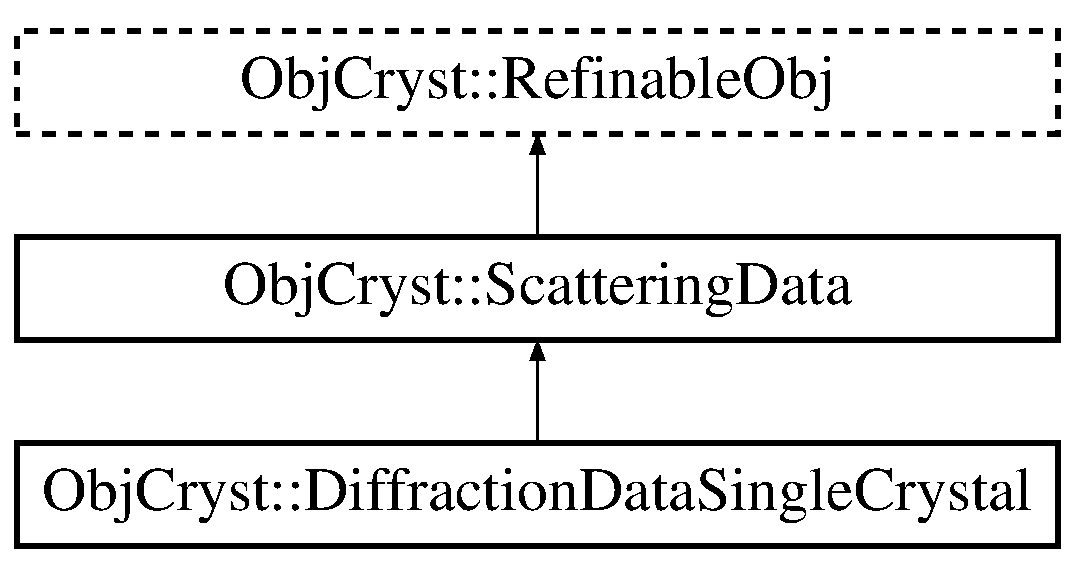
\includegraphics[height=3.000000cm]{a00026}
\end{center}
\end{figure}
\subsubsection*{Public Member Functions}
\begin{DoxyCompactItemize}
\item 
{\bf Diffraction\-Data\-Single\-Crystal} (const bool regist=true)
\begin{DoxyCompactList}\small\item\em Default constructor. \end{DoxyCompactList}\item 
{\bf Diffraction\-Data\-Single\-Crystal} ({\bf Crystal} \&cryst, const bool regist=true)
\begin{DoxyCompactList}\small\item\em Constructor, with an assigned crystal structure. \end{DoxyCompactList}\item 
{\bf Diffraction\-Data\-Single\-Crystal} (const {\bf Diffraction\-Data\-Single\-Crystal} \&old)\label{a00026_a2fbe3262e7146a0c1057da102d0a9046}

\begin{DoxyCompactList}\small\item\em Copy constructor. \end{DoxyCompactList}\item 
virtual \\*
{\bf Diffraction\-Data\-Single\-Crystal} $\ast$ {\bf Create\-Copy} () const \label{a00026_a49d006a0476d72570352e1d169200845}

\begin{DoxyCompactList}\small\item\em So-\/called virtual copy constructor. \end{DoxyCompactList}\item 
virtual const string \& {\bf Get\-Class\-Name} () const 
\begin{DoxyCompactList}\small\item\em Name for this class (\char`\"{}\-Refinable\-Obj\char`\"{}, \char`\"{}\-Crystal\char`\"{},...). \end{DoxyCompactList}\item 
const Cryst\-Vector\-\_\-\-R\-E\-A\-L \& {\bf Get\-Icalc} () const 
\begin{DoxyCompactList}\small\item\em returns the calculated diffracted intensity. \end{DoxyCompactList}\item 
const Cryst\-Vector\-\_\-\-R\-E\-A\-L \& {\bf Get\-Iobs} () const \label{a00026_a75e80d760a8f540aae7a0b678f3d60c6}

\begin{DoxyCompactList}\small\item\em Return the array of observed intensities for all peaks. \end{DoxyCompactList}\item 
void {\bf Set\-Iobs} (const Cryst\-Vector\-\_\-\-R\-E\-A\-L \&)\label{a00026_aaa8dd9fa1a0f7b3b050c96540992cea1}

\begin{DoxyCompactList}\small\item\em Return the array of observed intensities for all peaks. \end{DoxyCompactList}\item 
const Cryst\-Vector\-\_\-\-R\-E\-A\-L \& {\bf Get\-Sigma} () const \label{a00026_aad718f90b34f9a544ba86d5f8b02f46b}

\begin{DoxyCompactList}\small\item\em Return the array of sigmas for observed intensities, for all peaks. \end{DoxyCompactList}\item 
void {\bf Set\-Sigma} (const Cryst\-Vector\-\_\-\-R\-E\-A\-L \&)\label{a00026_afec714c8df5dc6a7cf68858dbf70742b}

\begin{DoxyCompactList}\small\item\em Return the array of sigmas for observed intensities, for all peaks. \end{DoxyCompactList}\item 
void {\bf Set\-Iobs\-To\-Icalc} ()\label{a00026_aa741c9f638e305ca800cf4ce0e31a615}

\begin{DoxyCompactList}\small\item\em Set Iobs to current values of Icalc. Mostly used for tests. \end{DoxyCompactList}\item 
const Cryst\-Vector\-\_\-\-R\-E\-A\-L \& {\bf Get\-Weight} () const \label{a00026_ab602d46a7bb6020229b2f8587171ae6a}

\begin{DoxyCompactList}\small\item\em Return the weights (for each reflection) used for computing Rw. \end{DoxyCompactList}\item 
void {\bf Set\-Weight} (const Cryst\-Vector\-\_\-\-R\-E\-A\-L \&)\label{a00026_ad30750b0b14e9b01427c311af560705c}

\begin{DoxyCompactList}\small\item\em Change the weights (for each reflection) used for computing Rw. \end{DoxyCompactList}\item 
void {\bf Set\-Hkl\-Iobs} (const Cryst\-Vector\-\_\-long \&h, const Cryst\-Vector\-\_\-long \&k, const Cryst\-Vector\-\_\-long \&l, const Cryst\-Vector\-\_\-\-R\-E\-A\-L \&i\-Obs, const Cryst\-Vector\-\_\-\-R\-E\-A\-L \&sigma)
\begin{DoxyCompactList}\small\item\em input H,K,L, Iobs and Sigma \end{DoxyCompactList}\item 
void {\bf Import\-Hkl\-Iobs} (const string \&file\-Name, const long nb\-Refl, const int skip\-Lines=0)
\begin{DoxyCompactList}\small\item\em Import h,k,l,I from a file. \end{DoxyCompactList}\item 
void {\bf Import\-Hkl\-Iobs\-Sigma} (const string \&file\-Name, const long nb\-Refl, const int skip\-Lines=0)
\begin{DoxyCompactList}\small\item\em Import h,k,l,I,Sigma from a file. \end{DoxyCompactList}\item 
void {\bf Import\-Hkl\-Iobs\-Sigma\-Jana\-M91} (const string \&file\-Name)
\begin{DoxyCompactList}\small\item\em Import h,k,l,I,Sigma from a Jana98 '$\ast$.m91' file. \end{DoxyCompactList}\item 
void {\bf Import\-Hkl\-Iobs\-Group} (const string \&file\-Name, const unsigned int skip\-Lines=0)
\begin{DoxyCompactList}\small\item\em Import h,k,l and grouped intensities from a file. \end{DoxyCompactList}\item 
virtual R\-E\-A\-L {\bf Get\-Rw} () const 
\begin{DoxyCompactList}\small\item\em Return the \doxyref{Crystal}{p.}{a00020} R-\/factor (weighted) \end{DoxyCompactList}\item 
virtual R\-E\-A\-L {\bf Get\-R} () const 
\begin{DoxyCompactList}\small\item\em Return the \doxyref{Crystal}{p.}{a00020} R-\/factor (unweighted) \end{DoxyCompactList}\item 
virtual R\-E\-A\-L {\bf Get\-Chi2} () const 
\begin{DoxyCompactList}\small\item\em Return conventionnal Chi$^\wedge$2. \end{DoxyCompactList}\item 
virtual void {\bf Fit\-Scale\-Factor\-For\-Rw} () const 
\begin{DoxyCompactList}\small\item\em Compute the best scale factor minimising Rw. \end{DoxyCompactList}\item 
virtual void {\bf Fit\-Scale\-Factor\-For\-R} () const 
\begin{DoxyCompactList}\small\item\em Compute the best scale factor minimising R. \end{DoxyCompactList}\item 
virtual R\-E\-A\-L {\bf Get\-Best\-R\-Factor} () const 
\begin{DoxyCompactList}\small\item\em Compute the best scale factor to minimize R, apply this scale factor and return the R value obtained. \end{DoxyCompactList}\item 
virtual void {\bf Set\-Sigma\-To\-Sqrt\-Iobs} ()
\begin{DoxyCompactList}\small\item\em Set sigma for all observed intensities to sqrt(obs) \end{DoxyCompactList}\item 
virtual void {\bf Set\-Weight\-To\-Inv\-Sigma2} (const R\-E\-A\-L min\-Relat\-Sigma=1e-\/4)
\begin{DoxyCompactList}\small\item\em Set the weight for all observed intensities to 1/sigma$^\wedge$2. \end{DoxyCompactList}\item 
R\-E\-A\-L {\bf Get\-Scale\-Factor} () const \label{a00026_a92da5b55bca84f7923d117e0794d9689}

\begin{DoxyCompactList}\small\item\em Scale factor (applied to Icalc to match Iobs) \end{DoxyCompactList}\item 
virtual void {\bf Print\-Obs\-Data} () const 
\begin{DoxyCompactList}\small\item\em Print H, K, L Iobs sigma for all reflections. \end{DoxyCompactList}\item 
virtual void {\bf Print\-Obs\-Calc\-Data} () const \label{a00026_a17da834176b793bc5edb3915f243a960}

\begin{DoxyCompactList}\small\item\em \begin{DoxyVerb}Print H, K, L Iobs sigma Icalc for all reflections
\end{DoxyVerb}
 $\ast$\-Iobs and sigma (if given) are scaled to Icalc (if available). \end{DoxyCompactList}\item 
virtual void {\bfseries Set\-Use\-Only\-Low\-Angle\-Data} (const bool use\-Only\-Low\-Angle, const R\-E\-A\-L angle=0.)\label{a00026_abfcedd24e1485124423b6e14aafb2b55}

\item 
void {\bf Save\-H\-K\-L\-Iobs\-Icalc} (const string \&filename=\char`\"{}hkl\-Iobs\-Icalc.\-out\char`\"{})
\begin{DoxyCompactList}\small\item\em Save H,K,L Iobs Icalc to a file, text format, 3 columns theta Iobs Icalc. \end{DoxyCompactList}\item 
virtual void {\bf Global\-Opt\-Random\-Move} (const R\-E\-A\-L mutation\-Amplitude, const {\bf Ref\-Par\-Type} $\ast$type={\bf gp\-Ref\-Par\-Type\-Obj\-Cryst})
\begin{DoxyCompactList}\small\item\em Make a random move of the current configuration. \end{DoxyCompactList}\item 
virtual R\-E\-A\-L {\bf Get\-Log\-Likelihood} () const 
\begin{DoxyCompactList}\small\item\em Get -\/log(likelihood) of the current configuration for the object. \end{DoxyCompactList}\item 
virtual unsigned int {\bf Get\-Nb\-L\-S\-Q\-Function} () const \label{a00026_af3fbd99a3fc7abe6450d9adcb59fc314}

\begin{DoxyCompactList}\small\item\em Number of L\-S\-Q functions. \end{DoxyCompactList}\item 
virtual const Cryst\-Vector\-\_\-\-R\-E\-A\-L \& {\bf Get\-L\-S\-Q\-Calc} (const unsigned int) const \label{a00026_ad13c33ef47af441539b95e11b6347054}

\begin{DoxyCompactList}\small\item\em Get the current calculated value for the L\-S\-Q function. \end{DoxyCompactList}\item 
virtual const Cryst\-Vector\-\_\-\-R\-E\-A\-L \& {\bf Get\-L\-S\-Q\-Obs} (const unsigned int) const \label{a00026_a339318a2481faa122f22fce3fce08a70}

\begin{DoxyCompactList}\small\item\em Get the observed values for the L\-S\-Q function. \end{DoxyCompactList}\item 
virtual const Cryst\-Vector\-\_\-\-R\-E\-A\-L \& {\bf Get\-L\-S\-Q\-Weight} (const unsigned int) const \label{a00026_ab7ce20d0a0d849f2d0304c7abad11b7f}

\begin{DoxyCompactList}\small\item\em Get the weight values for the L\-S\-Q function. \end{DoxyCompactList}\item 
virtual void {\bf X\-M\-L\-Output} (ostream \&os, int indent=0) const 
\begin{DoxyCompactList}\small\item\em Output to stream in well-\/formed X\-M\-L. \end{DoxyCompactList}\item 
virtual void {\bf X\-M\-L\-Input} (istream \&is, const {\bf X\-M\-L\-Cryst\-Tag} \&tag)
\begin{DoxyCompactList}\small\item\em Input From stream. \end{DoxyCompactList}\item 
virtual const {\bf Radiation} \& {\bf Get\-Radiation} () const \label{a00026_a334973e747b95a62fb7b2fc67ebb40d3}

\begin{DoxyCompactList}\small\item\em Get the radiation object for this data. \end{DoxyCompactList}\item 
{\bf Radiation} \& {\bfseries Get\-Radiation} ()\label{a00026_aaf39551c91d7849d49604012eba2a10c}

\item 
virtual void {\bf Set\-Radiation\-Type} (const {\bf Radiation\-Type} radiation)\label{a00026_a3c96d35001fef3833731910f4ed4690f}

\begin{DoxyCompactList}\small\item\em Set \-: neutron or x-\/ray experiment ? Wavelength ? \end{DoxyCompactList}\item 
void {\bf Set\-Wavelength} (const R\-E\-A\-L)\label{a00026_a19d588f3fd7ca539d89d87e7420438e1}

\begin{DoxyCompactList}\small\item\em Set the (monochromatic) wavelength of the beam. \end{DoxyCompactList}\item 
void {\bf Set\-Wavelength} (const string \&X\-Ray\-Tube\-Element\-Name, const R\-E\-A\-L alpha2\-Alpha2ratio=0.\-5)
\begin{DoxyCompactList}\small\item\em \textbackslash{} brief Set X-\/\-Ray tube radiation. \end{DoxyCompactList}\item 
void {\bf Set\-Energy} (const R\-E\-A\-L)\label{a00026_a4fa3e393b4b643bd02d184c043954def}

\begin{DoxyCompactList}\small\item\em Set the (monochromatic) energy of the beam. \end{DoxyCompactList}\end{DoxyCompactItemize}
\subsubsection*{Private Member Functions}
\begin{DoxyCompactItemize}
\item 
virtual void {\bfseries Init\-Ref\-Par\-List} ()\label{a00026_afe663c6aa23f64956d0b985fea65a0a5}

\item 
void {\bf Calc\-Icalc} () const \label{a00026_ad8480ba2ebf761c8dafea7a8c05f2a33}

\begin{DoxyCompactList}\small\item\em Calc intensities. \end{DoxyCompactList}\item 
virtual Cryst\-Vector\-\_\-long {\bf Sort\-Reflection\-By\-Sin\-Theta\-Over\-Lambda} (const R\-E\-A\-L max\-Theta=-\/1.)
\item 
void {\bf Init\-Options} ()\label{a00026_a3eafc2c0206c365024f40d4302c1257f}

\begin{DoxyCompactList}\small\item\em Init options (currently only twinning). \end{DoxyCompactList}\item 
void {\bf Prepare\-Twinning\-Calc} () const 
\begin{DoxyCompactList}\small\item\em Determine the index of reflections to be summed because of twinning (Group\-Option==1) The reflections {\itshape must} have been sorted by increasing theta beforehand. \end{DoxyCompactList}\end{DoxyCompactItemize}
\subsubsection*{Private Attributes}
\begin{DoxyCompactItemize}
\item 
bool {\bf m\-Has\-Observed\-Data}\label{a00026_a6509d08699c990b10bacae56e1c81da9}

\begin{DoxyCompactList}\small\item\em Are there observed intensities ? \end{DoxyCompactList}\item 
Cryst\-Vector\-\_\-\-R\-E\-A\-L {\bf m\-Obs\-Intensity}
\begin{DoxyCompactList}\small\item\em Observed intensity (after A\-B\-S and L\-P corrections) \end{DoxyCompactList}\item 
Cryst\-Vector\-\_\-\-R\-E\-A\-L {\bf m\-Obs\-Sigma}\label{a00026_ac944ecba535c9edb0c19adc503e014ec}

\begin{DoxyCompactList}\small\item\em Sigma for observed intensities (either individual reflections or spectrum) \end{DoxyCompactList}\item 
Cryst\-Vector\-\_\-\-R\-E\-A\-L {\bf m\-Weight}\label{a00026_a5856abdb592d801b220d3833d9306d88}

\begin{DoxyCompactList}\small\item\em weight for computing R-\/\-Factor, for each observed value. \end{DoxyCompactList}\item 
Cryst\-Vector\-\_\-\-R\-E\-A\-L {\bf m\-Calc\-Intensity}\label{a00026_a41450ac0f53bff0e8672ac69a7f63795}

\begin{DoxyCompactList}\small\item\em Calculated intensities. \end{DoxyCompactList}\item 
R\-E\-A\-L {\bf m\-Scale\-Factor}
\begin{DoxyCompactList}\small\item\em Scale factor. \end{DoxyCompactList}\item 
R\-E\-A\-L {\bf m\-Chi2}\label{a00026_a1ec5ae2f5102440a06f436c06938d78a}

\begin{DoxyCompactList}\small\item\em Chi$^\wedge$2. \end{DoxyCompactList}\item 
{\bf Refinable\-Obj\-Clock} {\bf m\-Clock\-Icalc}\label{a00026_a92796e78d88ba827bc39fd9278ea0d2d}

\begin{DoxyCompactList}\small\item\em Last time Icalc was computed. \end{DoxyCompactList}\item 
{\bf Refinable\-Obj\-Clock} {\bf m\-Clock\-Scale\-Factor}\label{a00026_a082df0e2c370d12dae3e84ca4be0c985}

\begin{DoxyCompactList}\small\item\em Last modification of the scale factor. \end{DoxyCompactList}\item 
{\bf Refinable\-Obj\-Clock} {\bf m\-Clock\-Chi2}\label{a00026_a600bb857f6648a262adbaeae67acb119}

\begin{DoxyCompactList}\small\item\em Clock the last time Chi$^\wedge$2 was computed. \end{DoxyCompactList}\item 
{\bf Ref\-Obj\-Opt} {\bf m\-Group\-Option}\label{a00026_a2173fb98cd1d27617eb8305ef12ad607}

\begin{DoxyCompactList}\small\item\em Option for the type of grouping (0\-:no, 1\-:by theta values (twinning), 2\-:user-\/supplied groups) \end{DoxyCompactList}\item 
Cryst\-Vector\-\_\-\-R\-E\-A\-L {\bf m\-Group\-Iobs}\label{a00026_a40173c931093085373ad6fd304f202b8}

\begin{DoxyCompactList}\small\item\em The observed intensities summed on all reflections that are (or could be) overlapped dur to a twinning. \end{DoxyCompactList}\item 
Cryst\-Vector\-\_\-\-R\-E\-A\-L {\bf m\-Group\-Sigma}\label{a00026_ac741c4954e3b89b81693c80afaec1576}

\begin{DoxyCompactList}\small\item\em The uncertainty on observed grouped intensities. \end{DoxyCompactList}\item 
Cryst\-Vector\-\_\-\-R\-E\-A\-L {\bf m\-Group\-Icalc}\label{a00026_a079d62283adb291b74d6c19e5d114eb4}

\begin{DoxyCompactList}\small\item\em The calculated intensities summed on all reflections that are grouped. \end{DoxyCompactList}\item 
Cryst\-Vector\-\_\-\-R\-E\-A\-L {\bf m\-Group\-Weight}
\begin{DoxyCompactList}\small\item\em The weight on each reflection sum in case of grouped reflections. \end{DoxyCompactList}\item 
Cryst\-Vector\-\_\-long {\bf m\-Group\-Index}
\begin{DoxyCompactList}\small\item\em The index of reflections which need to be summed. \end{DoxyCompactList}\item 
long {\bf m\-Nb\-Group}\label{a00026_a3ebc7c0b1cd1a13247920f7264903009}

\begin{DoxyCompactList}\small\item\em Number of groups. \end{DoxyCompactList}\item 
long {\bf m\-Nb\-Group\-Used}\label{a00026_abc5c636a84c000d831fab9e506904077}

\begin{DoxyCompactList}\small\item\em Number of groups below max[sin(theta)/lambda]. \end{DoxyCompactList}\item 
{\bf Refinable\-Obj\-Clock} {\bf m\-Clock\-Prepare\-Twinning\-Corr}\label{a00026_a03be010eb090d416b9c191f37e876ae6}

\begin{DoxyCompactList}\small\item\em Clock for twinning, when the preparation of twinning correction was last made. \end{DoxyCompactList}\item 
{\bf Radiation} {\bfseries m\-Radiation}\label{a00026_a82c829f88648010c963ea6ca80f5916f}

\end{DoxyCompactItemize}
\subsubsection*{Additional Inherited Members}


\subsubsection{Detailed Description}
Diffraction\-Data object for Single \doxyref{Crystal}{p.}{a00020} analysis. 

Currently this handles only in the simplest way single crystal dat\-: ie only data which has been completely corrected for Lorentz/\-Polarization and absorption.

What needs to be developped\-: define the geometry of the experiment (incident and emerging angles), the polarization of the beam, etc... 

\subsubsection{Constructor \& Destructor Documentation}
\index{Obj\-Cryst\-::\-Diffraction\-Data\-Single\-Crystal@{Obj\-Cryst\-::\-Diffraction\-Data\-Single\-Crystal}!Diffraction\-Data\-Single\-Crystal@{Diffraction\-Data\-Single\-Crystal}}
\index{Diffraction\-Data\-Single\-Crystal@{Diffraction\-Data\-Single\-Crystal}!ObjCryst::DiffractionDataSingleCrystal@{Obj\-Cryst\-::\-Diffraction\-Data\-Single\-Crystal}}
\paragraph[{Diffraction\-Data\-Single\-Crystal}]{\setlength{\rightskip}{0pt plus 5cm}Obj\-Cryst\-::\-Diffraction\-Data\-Single\-Crystal\-::\-Diffraction\-Data\-Single\-Crystal (
\begin{DoxyParamCaption}
\item[{const bool}]{regist = {\ttfamily true}}
\end{DoxyParamCaption}
)}\label{a00026_ab182bcffdd5cded6e7bd536bc71a3241}


Default constructor. 


\begin{DoxyParams}{Parameters}
{\em regist,\-:} & if false, do not add to the global registry of single crystal data or refinable objects -\/ this is only useful for data to be used internally only.\\
\hline
\end{DoxyParams}
\begin{DoxyRefDesc}{Deprecated}
\item[{\bf Deprecated}]Use the constructor passing a crystal structure instead. \end{DoxyRefDesc}
\index{Obj\-Cryst\-::\-Diffraction\-Data\-Single\-Crystal@{Obj\-Cryst\-::\-Diffraction\-Data\-Single\-Crystal}!Diffraction\-Data\-Single\-Crystal@{Diffraction\-Data\-Single\-Crystal}}
\index{Diffraction\-Data\-Single\-Crystal@{Diffraction\-Data\-Single\-Crystal}!ObjCryst::DiffractionDataSingleCrystal@{Obj\-Cryst\-::\-Diffraction\-Data\-Single\-Crystal}}
\paragraph[{Diffraction\-Data\-Single\-Crystal}]{\setlength{\rightskip}{0pt plus 5cm}Obj\-Cryst\-::\-Diffraction\-Data\-Single\-Crystal\-::\-Diffraction\-Data\-Single\-Crystal (
\begin{DoxyParamCaption}
\item[{{\bf Crystal} \&}]{cryst, }
\item[{const bool}]{regist = {\ttfamily true}}
\end{DoxyParamCaption}
)}\label{a00026_a3fcfa9d8f263043025d4167001c2243f}


Constructor, with an assigned crystal structure. 


\begin{DoxyParams}{Parameters}
{\em regist,\-:} & if false, do not add to the global registry of single crystal data or refinable objects -\/ this is only useful for data to be used internally only. \\
\hline
\end{DoxyParams}


\subsubsection{Member Function Documentation}
\index{Obj\-Cryst\-::\-Diffraction\-Data\-Single\-Crystal@{Obj\-Cryst\-::\-Diffraction\-Data\-Single\-Crystal}!Fit\-Scale\-Factor\-For\-R@{Fit\-Scale\-Factor\-For\-R}}
\index{Fit\-Scale\-Factor\-For\-R@{Fit\-Scale\-Factor\-For\-R}!ObjCryst::DiffractionDataSingleCrystal@{Obj\-Cryst\-::\-Diffraction\-Data\-Single\-Crystal}}
\paragraph[{Fit\-Scale\-Factor\-For\-R}]{\setlength{\rightskip}{0pt plus 5cm}virtual void Obj\-Cryst\-::\-Diffraction\-Data\-Single\-Crystal\-::\-Fit\-Scale\-Factor\-For\-R (
\begin{DoxyParamCaption}
{}
\end{DoxyParamCaption}
) const\hspace{0.3cm}{\ttfamily [virtual]}}\label{a00026_a97e666eeeb9e3b97a36145415e3f959e}


Compute the best scale factor minimising R. 

The computed scale factor is {\itshape immediatly} applied to Icalc \index{Obj\-Cryst\-::\-Diffraction\-Data\-Single\-Crystal@{Obj\-Cryst\-::\-Diffraction\-Data\-Single\-Crystal}!Fit\-Scale\-Factor\-For\-Rw@{Fit\-Scale\-Factor\-For\-Rw}}
\index{Fit\-Scale\-Factor\-For\-Rw@{Fit\-Scale\-Factor\-For\-Rw}!ObjCryst::DiffractionDataSingleCrystal@{Obj\-Cryst\-::\-Diffraction\-Data\-Single\-Crystal}}
\paragraph[{Fit\-Scale\-Factor\-For\-Rw}]{\setlength{\rightskip}{0pt plus 5cm}virtual void Obj\-Cryst\-::\-Diffraction\-Data\-Single\-Crystal\-::\-Fit\-Scale\-Factor\-For\-Rw (
\begin{DoxyParamCaption}
{}
\end{DoxyParamCaption}
) const\hspace{0.3cm}{\ttfamily [virtual]}}\label{a00026_a82c8acf2a3f315091d97ad154a74e17b}


Compute the best scale factor minimising Rw. 

The computed scale factor is {\itshape immediatly} applied to Icalc \index{Obj\-Cryst\-::\-Diffraction\-Data\-Single\-Crystal@{Obj\-Cryst\-::\-Diffraction\-Data\-Single\-Crystal}!Get\-Best\-R\-Factor@{Get\-Best\-R\-Factor}}
\index{Get\-Best\-R\-Factor@{Get\-Best\-R\-Factor}!ObjCryst::DiffractionDataSingleCrystal@{Obj\-Cryst\-::\-Diffraction\-Data\-Single\-Crystal}}
\paragraph[{Get\-Best\-R\-Factor}]{\setlength{\rightskip}{0pt plus 5cm}virtual R\-E\-A\-L Obj\-Cryst\-::\-Diffraction\-Data\-Single\-Crystal\-::\-Get\-Best\-R\-Factor (
\begin{DoxyParamCaption}
{}
\end{DoxyParamCaption}
) const\hspace{0.3cm}{\ttfamily [virtual]}}\label{a00026_a9f4bedb3f24193c14a39ad97ef074948}


Compute the best scale factor to minimize R, apply this scale factor and return the R value obtained. 

\index{Obj\-Cryst\-::\-Diffraction\-Data\-Single\-Crystal@{Obj\-Cryst\-::\-Diffraction\-Data\-Single\-Crystal}!Get\-Chi2@{Get\-Chi2}}
\index{Get\-Chi2@{Get\-Chi2}!ObjCryst::DiffractionDataSingleCrystal@{Obj\-Cryst\-::\-Diffraction\-Data\-Single\-Crystal}}
\paragraph[{Get\-Chi2}]{\setlength{\rightskip}{0pt plus 5cm}virtual R\-E\-A\-L Obj\-Cryst\-::\-Diffraction\-Data\-Single\-Crystal\-::\-Get\-Chi2 (
\begin{DoxyParamCaption}
{}
\end{DoxyParamCaption}
) const\hspace{0.3cm}{\ttfamily [virtual]}}\label{a00026_a406a2e413ed8c0a6afd92f384246d36c}


Return conventionnal Chi$^\wedge$2. 

\begin{DoxyReturn}{Returns}
$ \chi^2 = \sum_i w_i \left(I_i^{obs}-I_i^{calc} \right)^2 $ 
\end{DoxyReturn}
\index{Obj\-Cryst\-::\-Diffraction\-Data\-Single\-Crystal@{Obj\-Cryst\-::\-Diffraction\-Data\-Single\-Crystal}!Get\-Class\-Name@{Get\-Class\-Name}}
\index{Get\-Class\-Name@{Get\-Class\-Name}!ObjCryst::DiffractionDataSingleCrystal@{Obj\-Cryst\-::\-Diffraction\-Data\-Single\-Crystal}}
\paragraph[{Get\-Class\-Name}]{\setlength{\rightskip}{0pt plus 5cm}virtual const string\& Obj\-Cryst\-::\-Diffraction\-Data\-Single\-Crystal\-::\-Get\-Class\-Name (
\begin{DoxyParamCaption}
{}
\end{DoxyParamCaption}
) const\hspace{0.3cm}{\ttfamily [virtual]}}\label{a00026_a05b1f448a143ad61036f001d09a3509f}


Name for this class (\char`\"{}\-Refinable\-Obj\char`\"{}, \char`\"{}\-Crystal\char`\"{},...). 

This is only useful to distinguish different classes when picking up objects from the \doxyref{Refinable\-Obj}{p.}{a00071} Global Registry 

Reimplemented from {\bf Obj\-Cryst\-::\-Refinable\-Obj} \doxyref{}{p.}{a00071_a62968d90a7a3080738b363934616c019}.

\index{Obj\-Cryst\-::\-Diffraction\-Data\-Single\-Crystal@{Obj\-Cryst\-::\-Diffraction\-Data\-Single\-Crystal}!Get\-Icalc@{Get\-Icalc}}
\index{Get\-Icalc@{Get\-Icalc}!ObjCryst::DiffractionDataSingleCrystal@{Obj\-Cryst\-::\-Diffraction\-Data\-Single\-Crystal}}
\paragraph[{Get\-Icalc}]{\setlength{\rightskip}{0pt plus 5cm}const Cryst\-Vector\-\_\-\-R\-E\-A\-L\& Obj\-Cryst\-::\-Diffraction\-Data\-Single\-Crystal\-::\-Get\-Icalc (
\begin{DoxyParamCaption}
{}
\end{DoxyParamCaption}
) const}\label{a00026_a5aade79d8baf1b770ab82af93fd244e6}


returns the calculated diffracted intensity. 

This is an array of calculated intensities for each reflections in the single crystal case, and the array with the full powder powder profile for powder diffraction. \index{Obj\-Cryst\-::\-Diffraction\-Data\-Single\-Crystal@{Obj\-Cryst\-::\-Diffraction\-Data\-Single\-Crystal}!Get\-Log\-Likelihood@{Get\-Log\-Likelihood}}
\index{Get\-Log\-Likelihood@{Get\-Log\-Likelihood}!ObjCryst::DiffractionDataSingleCrystal@{Obj\-Cryst\-::\-Diffraction\-Data\-Single\-Crystal}}
\paragraph[{Get\-Log\-Likelihood}]{\setlength{\rightskip}{0pt plus 5cm}virtual R\-E\-A\-L Obj\-Cryst\-::\-Diffraction\-Data\-Single\-Crystal\-::\-Get\-Log\-Likelihood (
\begin{DoxyParamCaption}
{}
\end{DoxyParamCaption}
) const\hspace{0.3cm}{\ttfamily [virtual]}}\label{a00026_ad42c5159763eb136fadfb653067d1a7b}


Get -\/log(likelihood) of the current configuration for the object. 

By default (no likelihood evaluation available), this is equal to 0.

This call should not be recursive, it is the task of the algorithm to get the sum of likelihoods for all objects invlolved.

\begin{DoxyNote}{Note}
contrary to the old \char`\"{}\-Cost Function\char`\"{} approach, with log(\-Likelihood) there is no 'choice' of cost function, so that it is the task of the object to give the optimized likelihood (possibly with user options).
\end{DoxyNote}
\begin{DoxyWarning}{Warning}
\-: this is in under heavy development, so expect changes... 
\end{DoxyWarning}


Reimplemented from {\bf Obj\-Cryst\-::\-Refinable\-Obj} \doxyref{}{p.}{a00071_a9a9a5ea2b997cd36b44ed35c2bab3245}.

\index{Obj\-Cryst\-::\-Diffraction\-Data\-Single\-Crystal@{Obj\-Cryst\-::\-Diffraction\-Data\-Single\-Crystal}!Get\-R@{Get\-R}}
\index{Get\-R@{Get\-R}!ObjCryst::DiffractionDataSingleCrystal@{Obj\-Cryst\-::\-Diffraction\-Data\-Single\-Crystal}}
\paragraph[{Get\-R}]{\setlength{\rightskip}{0pt plus 5cm}virtual R\-E\-A\-L Obj\-Cryst\-::\-Diffraction\-Data\-Single\-Crystal\-::\-Get\-R (
\begin{DoxyParamCaption}
{}
\end{DoxyParamCaption}
) const\hspace{0.3cm}{\ttfamily [virtual]}}\label{a00026_a52253e2e3a9e0e1a8200c6e042d6f8c9}


Return the \doxyref{Crystal}{p.}{a00020} R-\/factor (unweighted) 

\begin{DoxyReturn}{Returns}
$ R= \sqrt {\frac{\sum_i \left( I_i^{obs}-I_i^{calc} \right)^2} {\sum_i (I_i^{obs})^2} }$ 
\end{DoxyReturn}
\index{Obj\-Cryst\-::\-Diffraction\-Data\-Single\-Crystal@{Obj\-Cryst\-::\-Diffraction\-Data\-Single\-Crystal}!Get\-Rw@{Get\-Rw}}
\index{Get\-Rw@{Get\-Rw}!ObjCryst::DiffractionDataSingleCrystal@{Obj\-Cryst\-::\-Diffraction\-Data\-Single\-Crystal}}
\paragraph[{Get\-Rw}]{\setlength{\rightskip}{0pt plus 5cm}virtual R\-E\-A\-L Obj\-Cryst\-::\-Diffraction\-Data\-Single\-Crystal\-::\-Get\-Rw (
\begin{DoxyParamCaption}
{}
\end{DoxyParamCaption}
) const\hspace{0.3cm}{\ttfamily [virtual]}}\label{a00026_addee789ac9e373d7080bd0fc395e68e8}


Return the \doxyref{Crystal}{p.}{a00020} R-\/factor (weighted) 

\begin{DoxyReturn}{Returns}
$ R_{w}= \sqrt {\frac{\sum_i w_i\left( I_i^{obs}-I_i^{calc} \right)^2} {\sum_i w_i (I_i^{obs})^2} }$ 
\end{DoxyReturn}
\index{Obj\-Cryst\-::\-Diffraction\-Data\-Single\-Crystal@{Obj\-Cryst\-::\-Diffraction\-Data\-Single\-Crystal}!Global\-Opt\-Random\-Move@{Global\-Opt\-Random\-Move}}
\index{Global\-Opt\-Random\-Move@{Global\-Opt\-Random\-Move}!ObjCryst::DiffractionDataSingleCrystal@{Obj\-Cryst\-::\-Diffraction\-Data\-Single\-Crystal}}
\paragraph[{Global\-Opt\-Random\-Move}]{\setlength{\rightskip}{0pt plus 5cm}virtual void Obj\-Cryst\-::\-Diffraction\-Data\-Single\-Crystal\-::\-Global\-Opt\-Random\-Move (
\begin{DoxyParamCaption}
\item[{const R\-E\-A\-L}]{mutation\-Amplitude, }
\item[{const {\bf Ref\-Par\-Type} $\ast$}]{type = {\ttfamily {\bf gp\-Ref\-Par\-Type\-Obj\-Cryst}}}
\end{DoxyParamCaption}
)\hspace{0.3cm}{\ttfamily [virtual]}}\label{a00026_a9f19efd0a77a471666ddd5b4be421ffa}


Make a random move of the current configuration. 

This is for global optimization algorithms. the moves for each parameter are less than their global optimization step, multiplied by the mutation amplitude.

\begin{DoxyWarning}{Warning}
\-: this makes a random move for the parameter declared for this object, and it is the duty of the object to decide whether the included objects should be moved and how. (eg an algorithm should only call for a move with the top object, and this object decides how he and his sub-\/objects moves). By default (\doxyref{Refinable\-Obj}{p.}{a00071} implementation) all included objects are moved recursively.
\end{DoxyWarning}
\doxyref{Refinable\-Obj}{p.}{a00071}\-:\-: 
\begin{DoxyParams}{Parameters}
{\em mutation\-Amplitude,\-:} & multiplier for the maximum move amplitude, for all parameters \\
\hline
{\em type,\-:} & restrain the change exclusively to parameters of a given type (same type or descendant from this \doxyref{Ref\-Par\-Type}{p.}{a00080}). \\
\hline
\end{DoxyParams}


Reimplemented from {\bf Obj\-Cryst\-::\-Refinable\-Obj} \doxyref{}{p.}{a00071_a18375c8525ae38c481ba77e9cf9d67c1}.

\index{Obj\-Cryst\-::\-Diffraction\-Data\-Single\-Crystal@{Obj\-Cryst\-::\-Diffraction\-Data\-Single\-Crystal}!Import\-Hkl\-Iobs@{Import\-Hkl\-Iobs}}
\index{Import\-Hkl\-Iobs@{Import\-Hkl\-Iobs}!ObjCryst::DiffractionDataSingleCrystal@{Obj\-Cryst\-::\-Diffraction\-Data\-Single\-Crystal}}
\paragraph[{Import\-Hkl\-Iobs}]{\setlength{\rightskip}{0pt plus 5cm}void Obj\-Cryst\-::\-Diffraction\-Data\-Single\-Crystal\-::\-Import\-Hkl\-Iobs (
\begin{DoxyParamCaption}
\item[{const string \&}]{file\-Name, }
\item[{const long}]{nb\-Refl, }
\item[{const int}]{skip\-Lines = {\ttfamily 0}}
\end{DoxyParamCaption}
)}\label{a00026_ac306439389c8eab225dd8dd87aa8f189}


Import h,k,l,I from a file. 

$\ast$\-The file is assumed to correspond to a single crystal diffraction file. 
\begin{DoxyParams}{Parameters}
{\em file\-Name} & The name of the data file. This file should be formatted $\ast$with H,k,l, Iobs separated by spaces. \\
\hline
{\em nb\-Refl} & The number of reflections to extract. \\
\hline
{\em skip\-Lines} & The number of lines to skip at the beginning of the file. \\
\hline
\end{DoxyParams}
\index{Obj\-Cryst\-::\-Diffraction\-Data\-Single\-Crystal@{Obj\-Cryst\-::\-Diffraction\-Data\-Single\-Crystal}!Import\-Hkl\-Iobs\-Group@{Import\-Hkl\-Iobs\-Group}}
\index{Import\-Hkl\-Iobs\-Group@{Import\-Hkl\-Iobs\-Group}!ObjCryst::DiffractionDataSingleCrystal@{Obj\-Cryst\-::\-Diffraction\-Data\-Single\-Crystal}}
\paragraph[{Import\-Hkl\-Iobs\-Group}]{\setlength{\rightskip}{0pt plus 5cm}void Obj\-Cryst\-::\-Diffraction\-Data\-Single\-Crystal\-::\-Import\-Hkl\-Iobs\-Group (
\begin{DoxyParamCaption}
\item[{const string \&}]{file\-Name, }
\item[{const unsigned int}]{skip\-Lines = {\ttfamily 0}}
\end{DoxyParamCaption}
)}\label{a00026_af590310eb70814be523947dc7ddc695c}


Import h,k,l and grouped intensities from a file. 

$\ast$\-The file is assumed to correspond to a single crystal diffraction file. 
\begin{DoxyParams}{Parameters}
{\em file\-Name} & The name of the data file. This file should be formatted $\ast$with H,k,l, Iobs separated by spaces. \\
\hline
{\em skip\-Lines} & The number of lines to skip at the beginning of the file.\\
\hline
\end{DoxyParams}
File format (the reflection which has an intensity entry marks the end of the group) h k l Igroup -\/2 4 2 -\/2 -\/4 2 100.\-4 2 -\/4 1 2 4 1 193.\-2 ... \index{Obj\-Cryst\-::\-Diffraction\-Data\-Single\-Crystal@{Obj\-Cryst\-::\-Diffraction\-Data\-Single\-Crystal}!Import\-Hkl\-Iobs\-Sigma@{Import\-Hkl\-Iobs\-Sigma}}
\index{Import\-Hkl\-Iobs\-Sigma@{Import\-Hkl\-Iobs\-Sigma}!ObjCryst::DiffractionDataSingleCrystal@{Obj\-Cryst\-::\-Diffraction\-Data\-Single\-Crystal}}
\paragraph[{Import\-Hkl\-Iobs\-Sigma}]{\setlength{\rightskip}{0pt plus 5cm}void Obj\-Cryst\-::\-Diffraction\-Data\-Single\-Crystal\-::\-Import\-Hkl\-Iobs\-Sigma (
\begin{DoxyParamCaption}
\item[{const string \&}]{file\-Name, }
\item[{const long}]{nb\-Refl, }
\item[{const int}]{skip\-Lines = {\ttfamily 0}}
\end{DoxyParamCaption}
)}\label{a00026_a041f22715b9b4d1f2beb2b7e387fa682}


Import h,k,l,I,Sigma from a file. 

$\ast$\-The file is assumed to correspond to a single crystal diffraction file. 
\begin{DoxyParams}{Parameters}
{\em file\-Name} & The name of the data file. This file should be formatted $\ast$with H,k,l, Iobs and Sigma separated by spaces. \\
\hline
{\em nb\-Refl} & The number of reflections to extract. \\
\hline
{\em skip\-Lines} & The number of lines to skip at the beginning of the file. \\
\hline
\end{DoxyParams}
\index{Obj\-Cryst\-::\-Diffraction\-Data\-Single\-Crystal@{Obj\-Cryst\-::\-Diffraction\-Data\-Single\-Crystal}!Import\-Hkl\-Iobs\-Sigma\-Jana\-M91@{Import\-Hkl\-Iobs\-Sigma\-Jana\-M91}}
\index{Import\-Hkl\-Iobs\-Sigma\-Jana\-M91@{Import\-Hkl\-Iobs\-Sigma\-Jana\-M91}!ObjCryst::DiffractionDataSingleCrystal@{Obj\-Cryst\-::\-Diffraction\-Data\-Single\-Crystal}}
\paragraph[{Import\-Hkl\-Iobs\-Sigma\-Jana\-M91}]{\setlength{\rightskip}{0pt plus 5cm}void Obj\-Cryst\-::\-Diffraction\-Data\-Single\-Crystal\-::\-Import\-Hkl\-Iobs\-Sigma\-Jana\-M91 (
\begin{DoxyParamCaption}
\item[{const string \&}]{file\-Name}
\end{DoxyParamCaption}
)}\label{a00026_a5721769a1b4a8e33664c3b0867c05086}


Import h,k,l,I,Sigma from a Jana98 '$\ast$.m91' file. 

$\ast$\-The file is assumed to correspond to a single crystal diffraction file. 
\begin{DoxyParams}{Parameters}
{\em file\-Name} & The name of the data file. \\
\hline
\end{DoxyParams}
\index{Obj\-Cryst\-::\-Diffraction\-Data\-Single\-Crystal@{Obj\-Cryst\-::\-Diffraction\-Data\-Single\-Crystal}!Prepare\-Twinning\-Calc@{Prepare\-Twinning\-Calc}}
\index{Prepare\-Twinning\-Calc@{Prepare\-Twinning\-Calc}!ObjCryst::DiffractionDataSingleCrystal@{Obj\-Cryst\-::\-Diffraction\-Data\-Single\-Crystal}}
\paragraph[{Prepare\-Twinning\-Calc}]{\setlength{\rightskip}{0pt plus 5cm}void Obj\-Cryst\-::\-Diffraction\-Data\-Single\-Crystal\-::\-Prepare\-Twinning\-Calc (
\begin{DoxyParamCaption}
{}
\end{DoxyParamCaption}
) const\hspace{0.3cm}{\ttfamily [private]}}\label{a00026_a7cc9b7b685ef9031f6e6176a5da1ed63}


Determine the index of reflections to be summed because of twinning (Group\-Option==1) The reflections {\itshape must} have been sorted by increasing theta beforehand. 

\index{Obj\-Cryst\-::\-Diffraction\-Data\-Single\-Crystal@{Obj\-Cryst\-::\-Diffraction\-Data\-Single\-Crystal}!Print\-Obs\-Data@{Print\-Obs\-Data}}
\index{Print\-Obs\-Data@{Print\-Obs\-Data}!ObjCryst::DiffractionDataSingleCrystal@{Obj\-Cryst\-::\-Diffraction\-Data\-Single\-Crystal}}
\paragraph[{Print\-Obs\-Data}]{\setlength{\rightskip}{0pt plus 5cm}virtual void Obj\-Cryst\-::\-Diffraction\-Data\-Single\-Crystal\-::\-Print\-Obs\-Data (
\begin{DoxyParamCaption}
{}
\end{DoxyParamCaption}
) const\hspace{0.3cm}{\ttfamily [virtual]}}\label{a00026_ad3c0c4361b81a2f7e786ed16968c6d88}


Print H, K, L Iobs sigma for all reflections. 

\index{Obj\-Cryst\-::\-Diffraction\-Data\-Single\-Crystal@{Obj\-Cryst\-::\-Diffraction\-Data\-Single\-Crystal}!Save\-H\-K\-L\-Iobs\-Icalc@{Save\-H\-K\-L\-Iobs\-Icalc}}
\index{Save\-H\-K\-L\-Iobs\-Icalc@{Save\-H\-K\-L\-Iobs\-Icalc}!ObjCryst::DiffractionDataSingleCrystal@{Obj\-Cryst\-::\-Diffraction\-Data\-Single\-Crystal}}
\paragraph[{Save\-H\-K\-L\-Iobs\-Icalc}]{\setlength{\rightskip}{0pt plus 5cm}void Obj\-Cryst\-::\-Diffraction\-Data\-Single\-Crystal\-::\-Save\-H\-K\-L\-Iobs\-Icalc (
\begin{DoxyParamCaption}
\item[{const string \&}]{filename = {\ttfamily \char`\"{}hklIobsIcalc.out\char`\"{}}}
\end{DoxyParamCaption}
)}\label{a00026_af220156c564b8d602b0c05ba222fba03}


Save H,K,L Iobs Icalc to a file, text format, 3 columns theta Iobs Icalc. 

If Iobs is missing, the column is omitted. \index{Obj\-Cryst\-::\-Diffraction\-Data\-Single\-Crystal@{Obj\-Cryst\-::\-Diffraction\-Data\-Single\-Crystal}!Set\-Hkl\-Iobs@{Set\-Hkl\-Iobs}}
\index{Set\-Hkl\-Iobs@{Set\-Hkl\-Iobs}!ObjCryst::DiffractionDataSingleCrystal@{Obj\-Cryst\-::\-Diffraction\-Data\-Single\-Crystal}}
\paragraph[{Set\-Hkl\-Iobs}]{\setlength{\rightskip}{0pt plus 5cm}void Obj\-Cryst\-::\-Diffraction\-Data\-Single\-Crystal\-::\-Set\-Hkl\-Iobs (
\begin{DoxyParamCaption}
\item[{const Cryst\-Vector\-\_\-long \&}]{h, }
\item[{const Cryst\-Vector\-\_\-long \&}]{k, }
\item[{const Cryst\-Vector\-\_\-long \&}]{l, }
\item[{const Cryst\-Vector\-\_\-\-R\-E\-A\-L \&}]{i\-Obs, }
\item[{const Cryst\-Vector\-\_\-\-R\-E\-A\-L \&}]{sigma}
\end{DoxyParamCaption}
)}\label{a00026_a0d13ab934c60c9bd0aebbb285a92c5cb}


input H,K,L, Iobs and Sigma 


\begin{DoxyParams}{Parameters}
{\em h,k,l,\-:} & R\-E\-A\-L arrays (vectors with Nb\-Refl elements -\/same size) $\ast$with the h, k and l coordinates of all reflections. \\
\hline
{\em iobs,sigma,\-:} & R\-E\-A\-L arrays (vectors with Nb\-Refl elements -\/same size) $\ast$with the Observed intensity and sigma for all reflections. \\
\hline
\end{DoxyParams}
\index{Obj\-Cryst\-::\-Diffraction\-Data\-Single\-Crystal@{Obj\-Cryst\-::\-Diffraction\-Data\-Single\-Crystal}!Set\-Sigma\-To\-Sqrt\-Iobs@{Set\-Sigma\-To\-Sqrt\-Iobs}}
\index{Set\-Sigma\-To\-Sqrt\-Iobs@{Set\-Sigma\-To\-Sqrt\-Iobs}!ObjCryst::DiffractionDataSingleCrystal@{Obj\-Cryst\-::\-Diffraction\-Data\-Single\-Crystal}}
\paragraph[{Set\-Sigma\-To\-Sqrt\-Iobs}]{\setlength{\rightskip}{0pt plus 5cm}virtual void Obj\-Cryst\-::\-Diffraction\-Data\-Single\-Crystal\-::\-Set\-Sigma\-To\-Sqrt\-Iobs (
\begin{DoxyParamCaption}
{}
\end{DoxyParamCaption}
)\hspace{0.3cm}{\ttfamily [virtual]}}\label{a00026_a55b89595cdd1305f69b725ba49dd9855}


Set sigma for all observed intensities to sqrt(obs) 

\index{Obj\-Cryst\-::\-Diffraction\-Data\-Single\-Crystal@{Obj\-Cryst\-::\-Diffraction\-Data\-Single\-Crystal}!Set\-Wavelength@{Set\-Wavelength}}
\index{Set\-Wavelength@{Set\-Wavelength}!ObjCryst::DiffractionDataSingleCrystal@{Obj\-Cryst\-::\-Diffraction\-Data\-Single\-Crystal}}
\paragraph[{Set\-Wavelength}]{\setlength{\rightskip}{0pt plus 5cm}void Obj\-Cryst\-::\-Diffraction\-Data\-Single\-Crystal\-::\-Set\-Wavelength (
\begin{DoxyParamCaption}
\item[{const string \&}]{X\-Ray\-Tube\-Element\-Name, }
\item[{const R\-E\-A\-L}]{alpha2\-Alpha2ratio = {\ttfamily 0.5}}
\end{DoxyParamCaption}
)}\label{a00026_a231437207dca7389aa593b1fd4fd9f1b}


\textbackslash{} brief Set X-\/\-Ray tube radiation. 


\begin{DoxyParams}{Parameters}
{\em X\-Ray\-Tube\-Element\-Name} & \-: name of the anticathode element name. Known $\ast$ones are Cr, Fe, Cu, Mo, Ag. \\
\hline
{\em alpha2\-Alpha2ratio,\-:} & Kalpha2/\-Kalpha1 ratio (0.\-5 by default)\\
\hline
\end{DoxyParams}
$\ast$the average wavelength is calculated $\ast$using the alpha2/alpha1 weight. All structure factors computation are made $\ast$using the average wavelength, and for powder diffraction, profiles are output $\ast$at the alpha1 and alpha2 ratio for the calculated pattern.

$\ast$\-N\-O\-T\-E \-: if the name of the wavelength is generic (eg\char`\"{}\-Cu\char`\"{}), $\ast$then the program considers that $\ast$there are both Alpha1 and Alpha2, and thus automatically changes the Wavelength\-Type $\ast$to W\-A\-V\-E\-L\-E\-N\-G\-T\-H\-\_\-\-A\-L\-P\-H\-A12. If instead either alpha1 or alpha2 (eg \char`\"{}\-Cu\-A1\char`\"{}) is asked for, $\ast$the Wavelength\-Type is set to W\-A\-V\-E\-L\-E\-N\-G\-T\-H\-\_\-\-M\-O\-N\-O\-C\-H\-R\-O\-M\-A\-T\-I\-C. In both cases, the radiation type is set to X-\/\-Ray. \index{Obj\-Cryst\-::\-Diffraction\-Data\-Single\-Crystal@{Obj\-Cryst\-::\-Diffraction\-Data\-Single\-Crystal}!Set\-Weight\-To\-Inv\-Sigma2@{Set\-Weight\-To\-Inv\-Sigma2}}
\index{Set\-Weight\-To\-Inv\-Sigma2@{Set\-Weight\-To\-Inv\-Sigma2}!ObjCryst::DiffractionDataSingleCrystal@{Obj\-Cryst\-::\-Diffraction\-Data\-Single\-Crystal}}
\paragraph[{Set\-Weight\-To\-Inv\-Sigma2}]{\setlength{\rightskip}{0pt plus 5cm}virtual void Obj\-Cryst\-::\-Diffraction\-Data\-Single\-Crystal\-::\-Set\-Weight\-To\-Inv\-Sigma2 (
\begin{DoxyParamCaption}
\item[{const R\-E\-A\-L}]{min\-Relat\-Sigma = {\ttfamily 1e-\/4}}
\end{DoxyParamCaption}
)\hspace{0.3cm}{\ttfamily [virtual]}}\label{a00026_a1b2bf6486f5030fa0cf59d057e8501b0}


Set the weight for all observed intensities to 1/sigma$^\wedge$2. 

$\ast$\-For sigmas which are smaller than min\-Relat\-Sigma times the max value of sigma, $\ast$the output weight is set to 0. \index{Obj\-Cryst\-::\-Diffraction\-Data\-Single\-Crystal@{Obj\-Cryst\-::\-Diffraction\-Data\-Single\-Crystal}!Sort\-Reflection\-By\-Sin\-Theta\-Over\-Lambda@{Sort\-Reflection\-By\-Sin\-Theta\-Over\-Lambda}}
\index{Sort\-Reflection\-By\-Sin\-Theta\-Over\-Lambda@{Sort\-Reflection\-By\-Sin\-Theta\-Over\-Lambda}!ObjCryst::DiffractionDataSingleCrystal@{Obj\-Cryst\-::\-Diffraction\-Data\-Single\-Crystal}}
\paragraph[{Sort\-Reflection\-By\-Sin\-Theta\-Over\-Lambda}]{\setlength{\rightskip}{0pt plus 5cm}virtual Cryst\-Vector\-\_\-long Obj\-Cryst\-::\-Diffraction\-Data\-Single\-Crystal\-::\-Sort\-Reflection\-By\-Sin\-Theta\-Over\-Lambda (
\begin{DoxyParamCaption}
\item[{const R\-E\-A\-L}]{max\-S\-T\-O\-L = {\ttfamily -\/1.}}
\end{DoxyParamCaption}
)\hspace{0.3cm}{\ttfamily [private]}, {\ttfamily [virtual]}}\label{a00026_aeac660426ee4c5aa52d494b449a164f9}
sort reflections by theta values (also get rid of [0,0,0] if present) If max\-S\-T\-O\-L $>$0, then only reflections where sin(theta)/lambda$<$max\-S\-T\-O\-L are kept \begin{DoxyReturn}{Returns}
an array with the subscript of the kept reflections (for inherited classes) 
\end{DoxyReturn}


Reimplemented from {\bf Obj\-Cryst\-::\-Scattering\-Data} \doxyref{}{p.}{a00089_a4b843c3350e25d4d0c52da3400768fb7}.

\index{Obj\-Cryst\-::\-Diffraction\-Data\-Single\-Crystal@{Obj\-Cryst\-::\-Diffraction\-Data\-Single\-Crystal}!X\-M\-L\-Input@{X\-M\-L\-Input}}
\index{X\-M\-L\-Input@{X\-M\-L\-Input}!ObjCryst::DiffractionDataSingleCrystal@{Obj\-Cryst\-::\-Diffraction\-Data\-Single\-Crystal}}
\paragraph[{X\-M\-L\-Input}]{\setlength{\rightskip}{0pt plus 5cm}virtual void Obj\-Cryst\-::\-Diffraction\-Data\-Single\-Crystal\-::\-X\-M\-L\-Input (
\begin{DoxyParamCaption}
\item[{istream \&}]{is, }
\item[{const {\bf X\-M\-L\-Cryst\-Tag} \&}]{tag}
\end{DoxyParamCaption}
)\hspace{0.3cm}{\ttfamily [virtual]}}\label{a00026_a3b1edc7d3c612fa20cb658ef1d084c00}


Input From stream. 

\begin{DoxyRefDesc}{Todo}
\item[{\bf Todo}]Add an bool X\-M\-L\-Input\-Tag(is,tag) function to recognize all the tags from the stream. So that each inherited class can use the X\-M\-L\-Input\-Tag function from its parent (ie take advantage of inheritance). The children class would first try to interpret the tag, then if unsuccessful would pass it to its parent (thus allowing overloading), etc... \end{DoxyRefDesc}


Reimplemented from {\bf Obj\-Cryst\-::\-Refinable\-Obj} \doxyref{}{p.}{a00071_ac13a4045c3f187879443c8615c38d623}.

\index{Obj\-Cryst\-::\-Diffraction\-Data\-Single\-Crystal@{Obj\-Cryst\-::\-Diffraction\-Data\-Single\-Crystal}!X\-M\-L\-Output@{X\-M\-L\-Output}}
\index{X\-M\-L\-Output@{X\-M\-L\-Output}!ObjCryst::DiffractionDataSingleCrystal@{Obj\-Cryst\-::\-Diffraction\-Data\-Single\-Crystal}}
\paragraph[{X\-M\-L\-Output}]{\setlength{\rightskip}{0pt plus 5cm}virtual void Obj\-Cryst\-::\-Diffraction\-Data\-Single\-Crystal\-::\-X\-M\-L\-Output (
\begin{DoxyParamCaption}
\item[{ostream \&}]{os, }
\item[{int}]{indent = {\ttfamily 0}}
\end{DoxyParamCaption}
) const\hspace{0.3cm}{\ttfamily [virtual]}}\label{a00026_a59dadf9f6dedc3a84e858ee96268526e}


Output to stream in well-\/formed X\-M\-L. 

\begin{DoxyRefDesc}{Todo}
\item[{\bf Todo}]Use inheritance.. as for X\-M\-L\-Input\-Tag()... \end{DoxyRefDesc}


Reimplemented from {\bf Obj\-Cryst\-::\-Refinable\-Obj} \doxyref{}{p.}{a00071_a7b9b6ed0f8dcf753d398c35e073de973}.



\subsubsection{Member Data Documentation}
\index{Obj\-Cryst\-::\-Diffraction\-Data\-Single\-Crystal@{Obj\-Cryst\-::\-Diffraction\-Data\-Single\-Crystal}!m\-Group\-Index@{m\-Group\-Index}}
\index{m\-Group\-Index@{m\-Group\-Index}!ObjCryst::DiffractionDataSingleCrystal@{Obj\-Cryst\-::\-Diffraction\-Data\-Single\-Crystal}}
\paragraph[{m\-Group\-Index}]{\setlength{\rightskip}{0pt plus 5cm}Cryst\-Vector\-\_\-long Obj\-Cryst\-::\-Diffraction\-Data\-Single\-Crystal\-::m\-Group\-Index\hspace{0.3cm}{\ttfamily [mutable]}, {\ttfamily [private]}}\label{a00026_a44eb55c673c51633521b38af7a489abe}


The index of reflections which need to be summed. 

They must have been sorted by increasing theta values. Each entry (the reflection index) marks the beginning of a new batch of reflections to be summed.

Here only the groups of reflections are {\itshape roughly} sorted by sin(theta)/lambda. It is assumed, howver, that grouped reflections are of approximately the same d\-\_\-hkl. After \doxyref{Scattering\-Data\-::\-Get\-Nb\-Refl\-Below\-Max\-Sin\-Theta\-Ov\-Lambda()}{p.}{a00089_aac8034f8b0f6980c619e595ce6ba1d65}, the number of groups for which {\itshape all} reflections are below the limit are taken into account for the statistics.

Note that  \doxyref{Diffraction\-Data\-Single\-Crystal\-::\-Sort\-Reflection\-By\-Sin\-Theta\-Over\-Lambda()}{p.}{a00026_aeac660426ee4c5aa52d494b449a164f9} is called (i.\-e. immediately after importing the reflections) \index{Obj\-Cryst\-::\-Diffraction\-Data\-Single\-Crystal@{Obj\-Cryst\-::\-Diffraction\-Data\-Single\-Crystal}!m\-Group\-Weight@{m\-Group\-Weight}}
\index{m\-Group\-Weight@{m\-Group\-Weight}!ObjCryst::DiffractionDataSingleCrystal@{Obj\-Cryst\-::\-Diffraction\-Data\-Single\-Crystal}}
\paragraph[{m\-Group\-Weight}]{\setlength{\rightskip}{0pt plus 5cm}Cryst\-Vector\-\_\-\-R\-E\-A\-L Obj\-Cryst\-::\-Diffraction\-Data\-Single\-Crystal\-::m\-Group\-Weight\hspace{0.3cm}{\ttfamily [mutable]}, {\ttfamily [private]}}\label{a00026_a800c45f228a27bf7915e312ae05048dc}


The weight on each reflection sum in case of grouped reflections. 

The sum is the inverse of the sum of all sigma$^\wedge$2 \index{Obj\-Cryst\-::\-Diffraction\-Data\-Single\-Crystal@{Obj\-Cryst\-::\-Diffraction\-Data\-Single\-Crystal}!m\-Obs\-Intensity@{m\-Obs\-Intensity}}
\index{m\-Obs\-Intensity@{m\-Obs\-Intensity}!ObjCryst::DiffractionDataSingleCrystal@{Obj\-Cryst\-::\-Diffraction\-Data\-Single\-Crystal}}
\paragraph[{m\-Obs\-Intensity}]{\setlength{\rightskip}{0pt plus 5cm}Cryst\-Vector\-\_\-\-R\-E\-A\-L Obj\-Cryst\-::\-Diffraction\-Data\-Single\-Crystal\-::m\-Obs\-Intensity\hspace{0.3cm}{\ttfamily [private]}}\label{a00026_a376708cee05a5d49ff22282748ef491b}


Observed intensity (after A\-B\-S and L\-P corrections) 

In the single crystal case, this is a list of intensity corresponding to (h,k,l). For a powder sample, this is a list of all peaks intensities. \index{Obj\-Cryst\-::\-Diffraction\-Data\-Single\-Crystal@{Obj\-Cryst\-::\-Diffraction\-Data\-Single\-Crystal}!m\-Scale\-Factor@{m\-Scale\-Factor}}
\index{m\-Scale\-Factor@{m\-Scale\-Factor}!ObjCryst::DiffractionDataSingleCrystal@{Obj\-Cryst\-::\-Diffraction\-Data\-Single\-Crystal}}
\paragraph[{m\-Scale\-Factor}]{\setlength{\rightskip}{0pt plus 5cm}R\-E\-A\-L Obj\-Cryst\-::\-Diffraction\-Data\-Single\-Crystal\-::m\-Scale\-Factor\hspace{0.3cm}{\ttfamily [mutable]}, {\ttfamily [private]}}\label{a00026_a4de0d528fa61c01cff4a0c78f5f5f1c3}


Scale factor. 

It is applied when computing intensities. The scale applies to intensities 

The documentation for this class was generated from the following file\-:\begin{DoxyCompactItemize}
\item 
Diffraction\-Data\-Single\-Crystal.\-h\end{DoxyCompactItemize}

\subsection{Obj\+Cryst\+:\+:Crystal\+P\+O\+V\+Ray\+Options Struct Reference}
\label{a00027}\index{Obj\+Cryst\+::\+Crystal\+P\+O\+V\+Ray\+Options@{Obj\+Cryst\+::\+Crystal\+P\+O\+V\+Ray\+Options}}


Class to store P\+O\+V-\/\+Ray output options.  


\subsubsection*{Public Attributes}
\begin{DoxyCompactItemize}
\item 
R\+E\+A\+L {\bf m\+Xmin}\label{a00027_a12de9193cec7f49031a0c250b01d80d2}

\begin{DoxyCompactList}\small\item\em Display limits in reduced coordinates. \end{DoxyCompactList}\item 
R\+E\+A\+L {\bfseries m\+Xmax}\label{a00027_a7338c4ff2ab270eafd33aa9a8cc2af9c}

\item 
R\+E\+A\+L {\bfseries m\+Ymin}\label{a00027_a1b91ecd75005d1fee4b4a665fb206ccf}

\item 
R\+E\+A\+L {\bfseries m\+Ymax}\label{a00027_a26b36c5944c2309ac04278a5e832d51b}

\item 
R\+E\+A\+L {\bfseries m\+Zmin}\label{a00027_a40b92456cf8a0d1d081315704ba4b4c1}

\item 
R\+E\+A\+L {\bfseries m\+Zmax}\label{a00027_a5edd263eb7efa26111d5361d676a9a92}

\item 
bool {\bf m\+Show\+Label}\label{a00027_a27d3053f6520b681d7db841b82fbaf92}

\begin{DoxyCompactList}\small\item\em Show labels ? \end{DoxyCompactList}\end{DoxyCompactItemize}


\subsubsection{Detailed Description}
Class to store P\+O\+V-\/\+Ray output options. 

The documentation for this struct was generated from the following file\+:\begin{DoxyCompactItemize}
\item 
General.\+h\end{DoxyCompactItemize}

\subsection{Cryst\+Array3\+D$<$ T $>$ Class Template Reference}
\label{a00028}\index{Cryst\+Array3\+D$<$ T $>$@{Cryst\+Array3\+D$<$ T $>$}}


3\+D Vector (Blitz++ mimic) for Obj\+Cryst++  


\subsubsection*{Public Member Functions}
\begin{DoxyCompactItemize}
\item 
{\bfseries Cryst\+Array3\+D} (const long z\+Size, const long y\+Size, const long x\+Size)\label{a00028_ad4ec05dc1208057b2ecabd8e8f2289f2}

\item 
{\bfseries Cryst\+Array3\+D} (const {\bf Cryst\+Array3\+D} \&old)\label{a00028_a7dabbca0551384e792bf898522073015}

\item 
void {\bfseries operator=} (const {\bf Cryst\+Array3\+D} \&old)\label{a00028_aafcbba0c2e2e64710f25d4706a18aff1}

\item 
void {\bfseries reference} ({\bf Cryst\+Array3\+D} \&old)\label{a00028_ac9c03573514355402c5da9c9bcb593aa}

\item 
long {\bfseries num\+Elements} () const \label{a00028_a188469a35af7b4060cfd8c0009b106ba}

\item 
T {\bfseries sum} () const \label{a00028_ad02f8908c0c683e6c5681a6251b3b3ef}

\item 
T {\bfseries min} () const \label{a00028_a0a0042adf867cfc3d5235dc7608524b4}

\item 
T {\bfseries max} () const \label{a00028_a160bf8c198eee8c7ad615b0d7e3b36c0}

\item 
long {\bfseries rows} () const \label{a00028_acb714370370850b93c3a9df1ff1ff714}

\item 
long {\bfseries cols} () const \label{a00028_a3b93ba2c331059226cf3ba71bf0ee073}

\item 
long {\bfseries depth} () const \label{a00028_a566512878ac310ca14aea3b1caab7928}

\item 
T $\ast$ {\bfseries data} ()\label{a00028_ac566777560641de36e2cf6184429c07a}

\item 
const T $\ast$ {\bfseries data} () const \label{a00028_abb62a47d55e244dd13e55a3c222003f5}

\item 
void {\bfseries resize} (const long z\+Size, const long y\+Size, const long x\+Size)\label{a00028_a5d2f2a6cb1815b7ccc26d7baa89f162f}

\item 
void {\bfseries resize\+And\+Preserve} (const long z\+Size, const long y\+Size, const long x\+Size)\label{a00028_aaaf6b3b51d14fb97f294f522ad88d129}

\item 
void {\bfseries operator=} (const T num)\label{a00028_a180dbc373520a3050f28c6d15f9d3127}

\item 
void {\bfseries operator$\ast$=} (const T num)\label{a00028_adbb26a696ca1426cbe68f0ac03c19e42}

\item 
void {\bfseries operator$\ast$=} (const {\bf Cryst\+Array3\+D} \&vect)\label{a00028_afa5e6378de16ffe99735641959ba8c71}

\item 
void {\bfseries operator/=} (const T num)\label{a00028_ae09d581b3bd395eef7bc5a3d0fe358d8}

\item 
void {\bfseries operator+=} (const T num)\label{a00028_a4c3a4526fc22e48a1794811b795b025e}

\item 
void {\bfseries operator-\/=} (const T num)\label{a00028_adcebc860353f85fa88001a5e12fc9d09}

\item 
T {\bfseries operator()} (const long i) const \label{a00028_a130625c785330dab16d6a656a30a6647}

\item 
T {\bfseries operator()} (const long depth, const long row, const long col) const \label{a00028_a9f5aa6cf692ba6755a87c750dba8f99d}

\item 
T \& {\bfseries operator()} (const long i)\label{a00028_a0f31bbbbee83042c88fe0437fb015892}

\item 
T \& {\bfseries operator()} (const long depth, const long row, const long col)\label{a00028_affb0c1dcd69cc4e0388f5b8bc4cdf6d2}

\end{DoxyCompactItemize}
\subsubsection*{Private Attributes}
\begin{DoxyCompactItemize}
\item 
T $\ast$ {\bfseries mp\+Data}\label{a00028_ab3d5b11715773cb704f6f4bded48d037}

\item 
long {\bfseries m\+Num\+Elements}\label{a00028_acfedf846348008cdc454680eab6fe39d}

\item 
long {\bfseries m\+X\+Size}\label{a00028_a74a117a6a8530bd27fdcb0970f7b63f4}

\item 
long {\bfseries m\+Y\+Size}\label{a00028_a3adeb73429e3f1c6ad733e79e928a2b4}

\item 
long {\bfseries m\+Z\+Size}\label{a00028_a4dd37579fffa5a1129658972816e4547}

\item 
bool {\bfseries m\+Is\+Areference}\label{a00028_a8e5ea60c4bd30f00c408df5c2e68f442}

\end{DoxyCompactItemize}


\subsubsection{Detailed Description}
\subsubsection*{template$<$class T$>$class Cryst\+Array3\+D$<$ T $>$}

3\+D Vector (Blitz++ mimic) for Obj\+Cryst++ 

The \doxyref{Cryst\+Vector}{p.}{a00030} library is not a new array computation library, despite the appearances. Obj\+Cryst++ should used the {\tt Blitz++ array library} , which yields excellent performance {\itshape and} simple array expressions. Unfortunately, the memory required to {\itshape compile} the library using gcc is far too high to be reasonable when using complex expressions and optimizing code. So until this has changed, The \doxyref{Cryst\+Vector}{p.}{a00030} and \doxyref{Cryst\+Matrix}{p.}{a00029} library have been created, and these emulate (supposedly exactly) the Blitz++ interface (but not the smart handling of mathematical expressions, so pointers must be used). For documentation about these two libraries you should read the {\tt Blitz++ documentation}. \doxyref{Cryst\+Vector}{p.}{a00030} and \doxyref{Cryst\+Matrix}{p.}{a00029} use the same kind of storage in memory.

You can use Cryst\+Array3\+D\+\_\+\+R\+E\+A\+L, Cryst\+Array3\+D\+\_\+long,etc... to declare 3\+D vectors. Macros ensure (well, should) ensure compatibility with Blitz++. (as of april 2001 support of blitz++ is broken). 

The documentation for this class was generated from the following file\+:\begin{DoxyCompactItemize}
\item 
Cryst\+Vector.\+h\end{DoxyCompactItemize}

\subsection{FormatHorizVector$<$ T $>$ Class Template Reference}
\label{a00029}\index{FormatHorizVector@{FormatHorizVector}}


Format vector as horiz array:.  
\subsubsection*{Public Member Functions}
\begin{DoxyCompactItemize}
\item 
{\bfseries FormatHorizVector} (const {\bf CrystVector}$<$ T $>$ \&fVect, const int width=10, const int precision=4)\label{a00029_a547a7cbadc52884eb1d0149ab62f6715}

\end{DoxyCompactItemize}
\subsubsection*{Public Attributes}
\begin{DoxyCompactItemize}
\item 
const {\bf CrystVector}$<$ T $>$ $\ast$ {\bfseries mpVectors}\label{a00029_a73b7421467798780d9c1d67424b3a876}

\item 
const int {\bfseries mWidth}\label{a00029_a3142a01d912b28c5fb2ff261915d80ba}

\item 
const int {\bfseries mPrecision}\label{a00029_ac1ca600c08c0dd17acd9d1d5721d4b57}

\end{DoxyCompactItemize}


\subsubsection{Detailed Description}
\subsubsection*{template$<$class T$>$ class FormatHorizVector$<$ T $>$}

Format vector as horiz array:. 
\begin{DoxyCode}
 os << FormatHorizVector<REAL>(vect,8,3);
\end{DoxyCode}
 

The documentation for this class was generated from the following file:\begin{DoxyCompactItemize}
\item 
VFNStreamFormat.h\end{DoxyCompactItemize}

\subsection{\-Format\-Int \-Class \-Reference}
\label{a00030}\index{\-Format\-Int@{\-Format\-Int}}


output a number as a formatted integer\-:  


\subsubsection*{\-Public \-Member \-Functions}
\begin{DoxyCompactItemize}
\item 
{\bfseries \-Format\-Int} (const long num, const int width=5)\label{a00030_a6c6098db56c85ccb7bfea46810d493c7}

\end{DoxyCompactItemize}
\subsubsection*{\-Public \-Attributes}
\begin{DoxyCompactItemize}
\item 
const long {\bfseries m\-Value}\label{a00030_a712caad7abfc009c6cff31d68b0dc4ed}

\item 
const int {\bfseries m\-Width}\label{a00030_aa98e381e2fb22e64fe2a61c8e56686ba}

\end{DoxyCompactItemize}


\subsubsection{\-Detailed \-Description}
output a number as a formatted integer\-: 


\begin{DoxyCode}
 os << FormatInt(mynumber,5);
\end{DoxyCode}
 

\-The documentation for this class was generated from the following file\-:\begin{DoxyCompactItemize}
\item 
\-V\-F\-N\-Stream\-Format.\-h\end{DoxyCompactItemize}

\subsection{Format\-String Class Reference}
\label{a00031}\index{Format\-String@{Format\-String}}


output a string with a fixed length (adding necessary space or removing excess characters) \-:  


\subsubsection*{Public Member Functions}
\begin{DoxyCompactItemize}
\item 
{\bfseries Format\-String} (const string \&str, const unsigned int width=5)\label{a00031_a89e88ecbdd91c8120ffbfbdc733c9b7b}

\item 
int {\bfseries length} () const \label{a00031_a8d9ccf3761a959d82bd705f601ae5360}

\end{DoxyCompactItemize}
\subsubsection*{Public Attributes}
\begin{DoxyCompactItemize}
\item 
string {\bfseries m\-String}\label{a00031_a08c22a7bd34d0bcf7c62147cff2a5e85}

\item 
const unsigned int {\bfseries m\-Width}\label{a00031_ae1191d6d25031c2d6e142ce989ff6c74}

\end{DoxyCompactItemize}


\subsubsection{Detailed Description}
output a string with a fixed length (adding necessary space or removing excess characters) \-: 


\begin{DoxyCode}
os << FormatString(myString,15);
\end{DoxyCode}
 

The documentation for this class was generated from the following file\-:\begin{DoxyCompactItemize}
\item 
V\-F\-N\-Stream\-Format.\-h\end{DoxyCompactItemize}

\subsection{Format\-Vert\-Vector$<$ T $>$ Class Template Reference}
\label{a00032}\index{Format\-Vert\-Vector$<$ T $>$@{Format\-Vert\-Vector$<$ T $>$}}


output one or several vectors as (a) column(s)\-:  


\subsubsection*{Public Member Functions}
\begin{DoxyCompactItemize}
\item 
{\bfseries Format\-Vert\-Vector} (const {\bf Cryst\-Vector}$<$ T $>$ \&f\-Vect, const int width=10, const int precision=4)\label{a00032_a98c9a8033613546d279d6fe85d110a58}

\item 
{\bfseries Format\-Vert\-Vector} (const {\bf Cryst\-Vector}$<$ T $>$ \&f\-Vect1, const {\bf Cryst\-Vector}$<$ T $>$ \&f\-Vect2, const int width=10, const int precision=4)\label{a00032_ae38ce51142cfd8d432f50f0b32914517}

\item 
{\bfseries Format\-Vert\-Vector} (const {\bf Cryst\-Vector}$<$ T $>$ \&f\-Vect1, const {\bf Cryst\-Vector}$<$ T $>$ \&f\-Vect2, const {\bf Cryst\-Vector}$<$ T $>$ \&f\-Vect3, const int width=10, const int precision=4)\label{a00032_ab06976e94d4a2d562c9a2ab379a03872}

\item 
{\bfseries Format\-Vert\-Vector} (const {\bf Cryst\-Vector}$<$ T $>$ \&f\-Vect1, const {\bf Cryst\-Vector}$<$ T $>$ \&f\-Vect2, const {\bf Cryst\-Vector}$<$ T $>$ \&f\-Vect3, const {\bf Cryst\-Vector}$<$ T $>$ \&f\-Vect4, const int width=10, const int precision=4)\label{a00032_a14984e7538dd2a3d46b796060ebc46cf}

\item 
{\bfseries Format\-Vert\-Vector} (const {\bf Cryst\-Vector}$<$ T $>$ \&f\-Vect1, const {\bf Cryst\-Vector}$<$ T $>$ \&f\-Vect2, const {\bf Cryst\-Vector}$<$ T $>$ \&f\-Vect3, const {\bf Cryst\-Vector}$<$ T $>$ \&f\-Vect4, const {\bf Cryst\-Vector}$<$ T $>$ \&f\-Vect5, const int width=10, const int precision=4)\label{a00032_af76de06df0cd4f9e3574ae1e3e1f24d3}

\item 
{\bfseries Format\-Vert\-Vector} (const {\bf Cryst\-Vector}$<$ T $>$ \&f\-Vect1, const {\bf Cryst\-Vector}$<$ T $>$ \&f\-Vect2, const {\bf Cryst\-Vector}$<$ T $>$ \&f\-Vect3, const {\bf Cryst\-Vector}$<$ T $>$ \&f\-Vect4, const {\bf Cryst\-Vector}$<$ T $>$ \&f\-Vect5, const {\bf Cryst\-Vector}$<$ T $>$ \&f\-Vect6, const int width=10, const int precision=4)\label{a00032_a41bd6bc4c5befd4e6fe1dade4ad87a57}

\item 
{\bfseries Format\-Vert\-Vector} (const {\bf Cryst\-Vector}$<$ T $>$ $\ast$p\-Vect, const int nb\-Vect, const int width=10, const int precision=4)\label{a00032_affdcb56b538bee3033cf89177e2eaa4e}

\item 
{\bfseries Format\-Vert\-Vector} (const {\bf Cryst\-Vector}$<$ T $>$ \&f\-Vect1, const {\bf Cryst\-Vector}$<$ T $>$ $\ast$p\-Vect, const int nb\-Vect, const int width=10, const int precision=4)\label{a00032_a6ca2c9a79903a6d4ba997d413ed8a238}

\end{DoxyCompactItemize}
\subsubsection*{Public Attributes}
\begin{DoxyCompactItemize}
\item 
const {\bf Cryst\-Vector}$<$ T $>$ $\ast$$\ast$ {\bfseries mp\-Vectors}\label{a00032_a373ff434e999897fb583bd4534f18167}

\item 
const int {\bfseries m\-Nb\-Vectors}\label{a00032_a4f7519552502a0968432d19fd2b0df4b}

\item 
const int {\bfseries m\-Width}\label{a00032_a0ea4d4aae7292f4e5421558156f4ba9e}

\item 
const int {\bfseries m\-Precision}\label{a00032_ad64d9a4b653d32862fa7abcc08972249}

\end{DoxyCompactItemize}


\subsubsection{Detailed Description}
\subsubsection*{template$<$class T$>$class Format\-Vert\-Vector$<$ T $>$}

output one or several vectors as (a) column(s)\-: 


\begin{DoxyCode}
   os << FormatVertVector<REAL>(vect,8,3);
   os << FormatVertVector<REAL>(vect1,vect2,vetc3,12,6);
   \textcolor{comment}{// For 7 vectors with width 12 and precision 4,}
   \textcolor{comment}{// pVect being a pointer to an array of 7 vectors:}
   os << FormatVertVector<REAL>(pVect,7,12,4);
\end{DoxyCode}
 

The documentation for this class was generated from the following file\-:\begin{DoxyCompactItemize}
\item 
V\-F\-N\-Stream\-Format.\-h\end{DoxyCompactItemize}

\subsection{Obj\+Cryst\+:\+:Molecule\+:\+:Flip\+Group Struct Reference}
\label{a00033}\index{Obj\+Cryst\+::\+Molecule\+::\+Flip\+Group@{Obj\+Cryst\+::\+Molecule\+::\+Flip\+Group}}


When 3(A1..1n) or more atoms are connected to a same atom A, it defines a 'flip' group, where it is possible to rotate bonds to their symmetric with respect to one plane defined by atoms Ai-\/\+A-\/\+Aj.  


\subsubsection*{Public Member Functions}
\begin{DoxyCompactItemize}
\item 
{\bf Flip\+Group} (const {\bf Mol\+Atom} \&at0, const {\bf Mol\+Atom} \&at1, const {\bf Mol\+Atom} \&at2)\label{a00033_ac065fb88e47795199d5e0c12dd53b839}

\begin{DoxyCompactList}\small\item\em Constructor, with the central atom. \end{DoxyCompactList}\end{DoxyCompactItemize}
\subsubsection*{Public Attributes}
\begin{DoxyCompactItemize}
\item 
const {\bf Mol\+Atom} $\ast$ {\bf mp\+Atom0}\label{a00033_abb2dfdd1e7967f5963b0fc0fdc079b4f}

\begin{DoxyCompactList}\small\item\em The atom which is an asymmetric center. \end{DoxyCompactList}\item 
const {\bf Mol\+Atom} $\ast$ {\bf mp\+Atom1}\label{a00033_ae503d7996cce85ae1acc1c4e07773fe6}

\begin{DoxyCompactList}\small\item\em The first atom defining the rotation axis. \end{DoxyCompactList}\item 
const {\bf Mol\+Atom} $\ast$ {\bf mp\+Atom2}\label{a00033_a3a7b47199e00b11ae9f039221bfd8283}

\begin{DoxyCompactList}\small\item\em The second atom defining the rotation axis. \end{DoxyCompactList}\item 
list$<$ pair$<$ const {\bf Mol\+Atom} \\*
$\ast$, set$<$ {\bf Mol\+Atom} $\ast$ $>$ $>$ $>$ {\bf mv\+Rotated\+Chain\+List}
\begin{DoxyCompactList}\small\item\em The set of atoms that are to be rotated during the flip. \end{DoxyCompactList}\item 
unsigned long {\bf m\+Nb\+Test}
\begin{DoxyCompactList}\small\item\em Number of times this flip has been tried, and the number of times it has been accepted. \end{DoxyCompactList}\item 
unsigned long {\bfseries m\+Nb\+Accept}\label{a00033_a0c6da7db2f88263d66a9fbba4ede927b}

\end{DoxyCompactItemize}


\subsubsection{Detailed Description}
When 3(A1..1n) or more atoms are connected to a same atom A, it defines a 'flip' group, where it is possible to rotate bonds to their symmetric with respect to one plane defined by atoms Ai-\/\+A-\/\+Aj. 

This is useful to flip the absolute configuration for asymmetric centers. Note that the bond is only rotated, so that the entire group is not mirrored (no absolute configuration is broken in the group).

Also, a \doxyref{Flip\+Group}{p.}{a00033} can correspond to a 180� rotation exchanging Ai and Aj (rotating the two chains around the bissecting angle of bonds A-\/\+Ai and A-\/\+Aj) 

\subsubsection{Member Data Documentation}
\index{Obj\+Cryst\+::\+Molecule\+::\+Flip\+Group@{Obj\+Cryst\+::\+Molecule\+::\+Flip\+Group}!m\+Nb\+Test@{m\+Nb\+Test}}
\index{m\+Nb\+Test@{m\+Nb\+Test}!Obj\+Cryst\+::\+Molecule\+::\+Flip\+Group@{Obj\+Cryst\+::\+Molecule\+::\+Flip\+Group}}
\paragraph[{m\+Nb\+Test}]{\setlength{\rightskip}{0pt plus 5cm}unsigned long Obj\+Cryst\+::\+Molecule\+::\+Flip\+Group\+::m\+Nb\+Test\hspace{0.3cm}{\ttfamily [mutable]}}\label{a00033_ac957576c4d555f0f32d76fedf11d1c3d}


Number of times this flip has been tried, and the number of times it has been accepted. 

Used in \doxyref{Molecule\+::\+Global\+Opt\+Random\+Move}{p.}{a00053_a11e623f6482b468f6dd05fc0ab2bbb24}, to avoid flips that break some restraint (and deciding which flips break some restraint is difficult before having a real conformation). \index{Obj\+Cryst\+::\+Molecule\+::\+Flip\+Group@{Obj\+Cryst\+::\+Molecule\+::\+Flip\+Group}!mv\+Rotated\+Chain\+List@{mv\+Rotated\+Chain\+List}}
\index{mv\+Rotated\+Chain\+List@{mv\+Rotated\+Chain\+List}!Obj\+Cryst\+::\+Molecule\+::\+Flip\+Group@{Obj\+Cryst\+::\+Molecule\+::\+Flip\+Group}}
\paragraph[{mv\+Rotated\+Chain\+List}]{\setlength{\rightskip}{0pt plus 5cm}list$<$pair$<$const {\bf Mol\+Atom} $\ast$,set$<${\bf Mol\+Atom} $\ast$$>$ $>$ $>$ Obj\+Cryst\+::\+Molecule\+::\+Flip\+Group\+::mv\+Rotated\+Chain\+List}\label{a00033_a30d77e3abea9f1bb27ffcd92dc1120cc}


The set of atoms that are to be rotated during the flip. 

The first atom is the one bonded to the central atom, whose bond will be flipped with respect to the plane defined by (at1,at0,at2).

However, if this atom is identical to mp\+Atom0, then this indicates that a 180� rotation exchanging atom1 and atom2 is to be performed. 

The documentation for this struct was generated from the following file\+:\begin{DoxyCompactItemize}
\item 
Molecule.\+h\end{DoxyCompactItemize}

\subsection{Format\+Float Class Reference}
\label{a00034}\index{Format\+Float@{Format\+Float}}


output a number as a formatted float\+:  


\subsubsection*{Public Member Functions}
\begin{DoxyCompactItemize}
\item 
{\bfseries Format\+Float} (const R\+E\+A\+L num, const int width=10, const int precision=4)\label{a00034_a9fbcfe7405d478396858e748dd7df56d}

\end{DoxyCompactItemize}
\subsubsection*{Public Attributes}
\begin{DoxyCompactItemize}
\item 
const R\+E\+A\+L {\bfseries m\+Value}\label{a00034_a09d44759a75e7d27abde5fb4d08870bd}

\item 
const int {\bfseries m\+Width}\label{a00034_a6933d0fb1fb1301fe9572e2048d06ade}

\item 
const int {\bfseries m\+Precision}\label{a00034_a2f9e8289795d3d9916873c105f0db4b3}

\end{DoxyCompactItemize}


\subsubsection{Detailed Description}
output a number as a formatted float\+: 


\begin{DoxyCode}
os << FormatFloat(mynumber,10,4); 
\end{DoxyCode}
 

The documentation for this class was generated from the following file\+:\begin{DoxyCompactItemize}
\item 
V\+F\+N\+Stream\+Format.\+h\end{DoxyCompactItemize}

\subsection{Format\+Horiz\+Vector$<$ T $>$ Class Template Reference}
\label{a00035}\index{Format\+Horiz\+Vector$<$ T $>$@{Format\+Horiz\+Vector$<$ T $>$}}


Format vector as horiz array\+:  


\subsubsection*{Public Member Functions}
\begin{DoxyCompactItemize}
\item 
{\bfseries Format\+Horiz\+Vector} (const {\bf Cryst\+Vector}$<$ T $>$ \&f\+Vect, const int width=10, const int precision=4)\label{a00035_a547a7cbadc52884eb1d0149ab62f6715}

\end{DoxyCompactItemize}
\subsubsection*{Public Attributes}
\begin{DoxyCompactItemize}
\item 
const {\bf Cryst\+Vector}$<$ T $>$ $\ast$ {\bfseries mp\+Vectors}\label{a00035_a73b7421467798780d9c1d67424b3a876}

\item 
const int {\bfseries m\+Width}\label{a00035_a3142a01d912b28c5fb2ff261915d80ba}

\item 
const int {\bfseries m\+Precision}\label{a00035_ac1ca600c08c0dd17acd9d1d5721d4b57}

\end{DoxyCompactItemize}


\subsubsection{Detailed Description}
\subsubsection*{template$<$class T$>$class Format\+Horiz\+Vector$<$ T $>$}

Format vector as horiz array\+: 


\begin{DoxyCode}
os << FormatHorizVector<REAL>(vect,8,3);
\end{DoxyCode}
 

The documentation for this class was generated from the following file\+:\begin{DoxyCompactItemize}
\item 
V\+F\+N\+Stream\+Format.\+h\end{DoxyCompactItemize}

\subsection{Format\-Horiz\-Vector$<$ T $>$ Class Template Reference}
\label{a00036}\index{Format\-Horiz\-Vector$<$ T $>$@{Format\-Horiz\-Vector$<$ T $>$}}


Format vector as horiz array\-:  


\subsubsection*{Public Member Functions}
\begin{DoxyCompactItemize}
\item 
{\bfseries Format\-Horiz\-Vector} (const {\bf Cryst\-Vector}$<$ T $>$ \&f\-Vect, const int width=10, const int precision=4)\label{a00036_a547a7cbadc52884eb1d0149ab62f6715}

\end{DoxyCompactItemize}
\subsubsection*{Public Attributes}
\begin{DoxyCompactItemize}
\item 
const {\bf Cryst\-Vector}$<$ T $>$ $\ast$ {\bfseries mp\-Vectors}\label{a00036_a73b7421467798780d9c1d67424b3a876}

\item 
const int {\bfseries m\-Width}\label{a00036_a3142a01d912b28c5fb2ff261915d80ba}

\item 
const int {\bfseries m\-Precision}\label{a00036_ac1ca600c08c0dd17acd9d1d5721d4b57}

\end{DoxyCompactItemize}


\subsubsection{Detailed Description}
\subsubsection*{template$<$class T$>$class Format\-Horiz\-Vector$<$ T $>$}

Format vector as horiz array\-: 


\begin{DoxyCode}
os << FormatHorizVector<REAL>(vect,8,3);
\end{DoxyCode}
 

The documentation for this class was generated from the following file\-:\begin{DoxyCompactItemize}
\item 
V\-F\-N\-Stream\-Format.\-h\end{DoxyCompactItemize}

\subsection{Format\+String Class Reference}
\label{a00037}\index{Format\+String@{Format\+String}}


output a string with a fixed length (adding necessary space or removing excess characters) \+:  


\subsubsection*{Public Member Functions}
\begin{DoxyCompactItemize}
\item 
{\bfseries Format\+String} (const string \&str, const unsigned int width=5)\label{a00037_a89e88ecbdd91c8120ffbfbdc733c9b7b}

\item 
int {\bfseries length} () const \label{a00037_a8d9ccf3761a959d82bd705f601ae5360}

\end{DoxyCompactItemize}
\subsubsection*{Public Attributes}
\begin{DoxyCompactItemize}
\item 
string {\bfseries m\+String}\label{a00037_a08c22a7bd34d0bcf7c62147cff2a5e85}

\item 
const unsigned int {\bfseries m\+Width}\label{a00037_ae1191d6d25031c2d6e142ce989ff6c74}

\end{DoxyCompactItemize}


\subsubsection{Detailed Description}
output a string with a fixed length (adding necessary space or removing excess characters) \+: 


\begin{DoxyCode}
os << FormatString(myString,15);
\end{DoxyCode}
 

The documentation for this class was generated from the following file\+:\begin{DoxyCompactItemize}
\item 
V\+F\+N\+Stream\+Format.\+h\end{DoxyCompactItemize}

\subsection{\-Obj\-Cryst\-:\-:\-Lorentz\-Corr \-Class \-Reference}
\label{a00038}\index{\-Obj\-Cryst\-::\-Lorentz\-Corr@{\-Obj\-Cryst\-::\-Lorentz\-Corr}}


\-Lorentz \-Correction.  


\-Inheritance diagram for \-Obj\-Cryst\-:\-:\-Lorentz\-Corr\-:\begin{figure}[H]
\begin{center}
\leavevmode
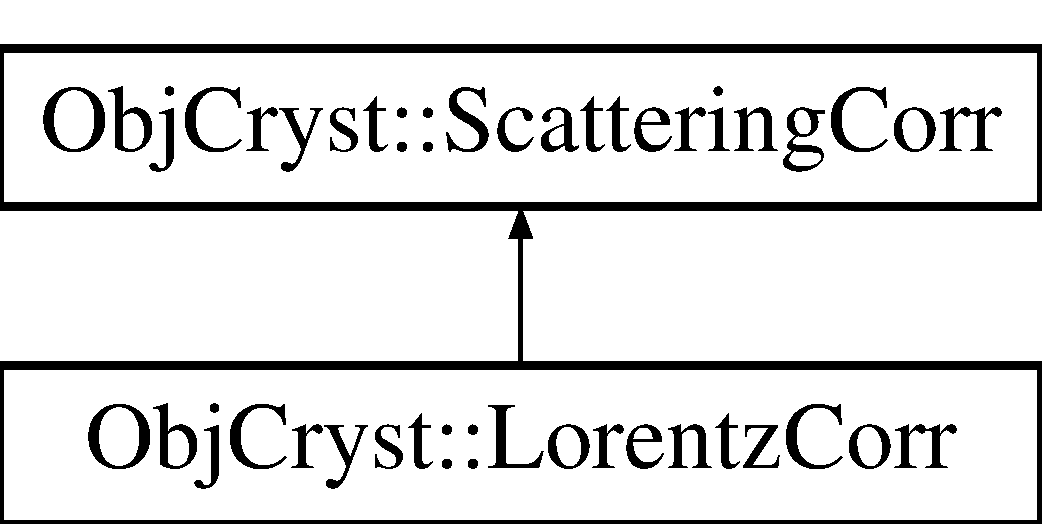
\includegraphics[height=2.000000cm]{a00038}
\end{center}
\end{figure}
\subsubsection*{\-Public \-Member \-Functions}
\begin{DoxyCompactItemize}
\item 
{\bfseries \-Lorentz\-Corr} (const {\bf \-Scattering\-Data} \&data)\label{a00038_a9f814b060cfafe4e829dc3977d9a7f1b}

\item 
virtual const string \& {\bf \-Get\-Name} () const \label{a00038_ab57782d9fe860701bb87309742afe2e5}

\begin{DoxyCompactList}\small\item\em \-Get the name of this object. \end{DoxyCompactList}\item 
virtual const string \& {\bf \-Get\-Class\-Name} () const \label{a00038_a740bd7f01b62a994ad5bc1c121d1e626}

\begin{DoxyCompactList}\small\item\em \-Get the name of the class. \end{DoxyCompactList}\end{DoxyCompactItemize}
\subsubsection*{\-Protected \-Member \-Functions}
\begin{DoxyCompactItemize}
\item 
virtual void {\bf \-Calc\-Corr} () const \label{a00038_adc247e6477f11474c542f2979984d238}

\begin{DoxyCompactList}\small\item\em \-Do the computation of corrected intensities. \end{DoxyCompactList}\end{DoxyCompactItemize}


\subsubsection{\-Detailed \-Description}
\-Lorentz \-Correction. 

\-So far, it only considers the correction for equatorial diffraction\-: $ L = \frac{1}{\sin(2\theta)} $ 

\-The documentation for this class was generated from the following file\-:\begin{DoxyCompactItemize}
\item 
\-Scattering\-Corr.\-h\end{DoxyCompactItemize}

\subsection{Format\-Vert\-Vector$<$ T $>$ Class Template Reference}
\label{a00039}\index{Format\-Vert\-Vector$<$ T $>$@{Format\-Vert\-Vector$<$ T $>$}}


output one or several vectors as (a) column(s)\-:  


\subsubsection*{Public Member Functions}
\begin{DoxyCompactItemize}
\item 
{\bfseries Format\-Vert\-Vector} (const {\bf Cryst\-Vector}$<$ T $>$ \&f\-Vect, const int width=10, const int precision=4)\label{a00039_a98c9a8033613546d279d6fe85d110a58}

\item 
{\bfseries Format\-Vert\-Vector} (const {\bf Cryst\-Vector}$<$ T $>$ \&f\-Vect1, const {\bf Cryst\-Vector}$<$ T $>$ \&f\-Vect2, const int width=10, const int precision=4)\label{a00039_ae38ce51142cfd8d432f50f0b32914517}

\item 
{\bfseries Format\-Vert\-Vector} (const {\bf Cryst\-Vector}$<$ T $>$ \&f\-Vect1, const {\bf Cryst\-Vector}$<$ T $>$ \&f\-Vect2, const {\bf Cryst\-Vector}$<$ T $>$ \&f\-Vect3, const int width=10, const int precision=4)\label{a00039_ab06976e94d4a2d562c9a2ab379a03872}

\item 
{\bfseries Format\-Vert\-Vector} (const {\bf Cryst\-Vector}$<$ T $>$ \&f\-Vect1, const {\bf Cryst\-Vector}$<$ T $>$ \&f\-Vect2, const {\bf Cryst\-Vector}$<$ T $>$ \&f\-Vect3, const {\bf Cryst\-Vector}$<$ T $>$ \&f\-Vect4, const int width=10, const int precision=4)\label{a00039_a14984e7538dd2a3d46b796060ebc46cf}

\item 
{\bfseries Format\-Vert\-Vector} (const {\bf Cryst\-Vector}$<$ T $>$ \&f\-Vect1, const {\bf Cryst\-Vector}$<$ T $>$ \&f\-Vect2, const {\bf Cryst\-Vector}$<$ T $>$ \&f\-Vect3, const {\bf Cryst\-Vector}$<$ T $>$ \&f\-Vect4, const {\bf Cryst\-Vector}$<$ T $>$ \&f\-Vect5, const int width=10, const int precision=4)\label{a00039_af76de06df0cd4f9e3574ae1e3e1f24d3}

\item 
{\bfseries Format\-Vert\-Vector} (const {\bf Cryst\-Vector}$<$ T $>$ \&f\-Vect1, const {\bf Cryst\-Vector}$<$ T $>$ \&f\-Vect2, const {\bf Cryst\-Vector}$<$ T $>$ \&f\-Vect3, const {\bf Cryst\-Vector}$<$ T $>$ \&f\-Vect4, const {\bf Cryst\-Vector}$<$ T $>$ \&f\-Vect5, const {\bf Cryst\-Vector}$<$ T $>$ \&f\-Vect6, const int width=10, const int precision=4)\label{a00039_a41bd6bc4c5befd4e6fe1dade4ad87a57}

\item 
{\bfseries Format\-Vert\-Vector} (const {\bf Cryst\-Vector}$<$ T $>$ $\ast$p\-Vect, const int nb\-Vect, const int width=10, const int precision=4)\label{a00039_affdcb56b538bee3033cf89177e2eaa4e}

\item 
{\bfseries Format\-Vert\-Vector} (const {\bf Cryst\-Vector}$<$ T $>$ \&f\-Vect1, const {\bf Cryst\-Vector}$<$ T $>$ $\ast$p\-Vect, const int nb\-Vect, const int width=10, const int precision=4)\label{a00039_a6ca2c9a79903a6d4ba997d413ed8a238}

\end{DoxyCompactItemize}
\subsubsection*{Public Attributes}
\begin{DoxyCompactItemize}
\item 
const {\bf Cryst\-Vector}$<$ T $>$ $\ast$$\ast$ {\bfseries mp\-Vectors}\label{a00039_a373ff434e999897fb583bd4534f18167}

\item 
const int {\bfseries m\-Nb\-Vectors}\label{a00039_a4f7519552502a0968432d19fd2b0df4b}

\item 
const int {\bfseries m\-Width}\label{a00039_a0ea4d4aae7292f4e5421558156f4ba9e}

\item 
const int {\bfseries m\-Precision}\label{a00039_ad64d9a4b653d32862fa7abcc08972249}

\end{DoxyCompactItemize}


\subsubsection{Detailed Description}
\subsubsection*{template$<$class T$>$class Format\-Vert\-Vector$<$ T $>$}

output one or several vectors as (a) column(s)\-: 


\begin{DoxyCode}
*  os << FormatVertVector<REAL>(vect,8,3);
*  os << FormatVertVector<REAL>(vect1,vect2,vetc3,12,6);
*  \textcolor{comment}{// For 7 vectors with width 12 and precision 4,}
*  \textcolor{comment}{// pVect being a pointer to an array of 7 vectors:}
*  os << FormatVertVector<REAL>(pVect,7,12,4);
* 
\end{DoxyCode}
 

The documentation for this class was generated from the following file\-:\begin{DoxyCompactItemize}
\item 
V\-F\-N\-Stream\-Format.\-h\end{DoxyCompactItemize}

\subsection{Obj\+Cryst\+:\+:Global\+Scattering\+Power Class Reference}
\label{a00040}\index{Obj\+Cryst\+::\+Global\+Scattering\+Power@{Obj\+Cryst\+::\+Global\+Scattering\+Power}}


Global Scattering Power.  


Inheritance diagram for Obj\+Cryst\+:\+:Global\+Scattering\+Power\+:\begin{figure}[H]
\begin{center}
\leavevmode
\includegraphics[height=3.000000cm]{a00040}
\end{center}
\end{figure}
\subsubsection*{Public Member Functions}
\begin{DoxyCompactItemize}
\item 
{\bfseries Global\+Scattering\+Power} (const {\bf Z\+Scatterer} \&scatt)\label{a00040_acb09756b2191173fdd48356c77e325bc}

\item 
{\bfseries Global\+Scattering\+Power} (const {\bf Global\+Scattering\+Power} \&old)\label{a00040_a9a494d9a254eaaf7bb1525bfb7a1ad14}

\item 
void {\bf Init} (const {\bf Z\+Scatterer} \&scatt)\label{a00040_a8f47e4dd26899ab2fcedd5f6b844317d}

\begin{DoxyCompactList}\small\item\em Re-\/initialize parameters (after using the default constructor). \end{DoxyCompactList}\item 
virtual Cryst\+Vector\+\_\+\+R\+E\+A\+L {\bf Get\+Scattering\+Factor} (const {\bf Scattering\+Data} \&data, const int spg\+Sym\+Pos\+Index=0) const 
\begin{DoxyCompactList}\small\item\em Get the Scattering factor for all reflections of a given \doxyref{Scattering\+Data}{p.}{a00095} object. \end{DoxyCompactList}\item 
virtual R\+E\+A\+L {\bf Get\+Forward\+Scattering\+Factor} (const {\bf Radiation\+Type}) const 
\begin{DoxyCompactList}\small\item\em Get the scattering factor at (0,0,0). \end{DoxyCompactList}\item 
virtual Cryst\+Vector\+\_\+\+R\+E\+A\+L {\bf Get\+Temperature\+Factor} (const {\bf Scattering\+Data} \&data, const int spg\+Sym\+Pos\+Index=0) const 
\begin{DoxyCompactList}\small\item\em Get the temperature factor for all reflections of a given \doxyref{Scattering\+Data}{p.}{a00095} object. \end{DoxyCompactList}\item 
virtual Cryst\+Matrix\+\_\+\+R\+E\+A\+L {\bf Get\+Resonant\+Scatt\+Fact\+Real} (const {\bf Scattering\+Data} \&data, const int spg\+Sym\+Pos\+Index=0) const 
\begin{DoxyCompactList}\small\item\em Get the real part of the resonant scattering factor. \end{DoxyCompactList}\item 
virtual Cryst\+Matrix\+\_\+\+R\+E\+A\+L {\bf Get\+Resonant\+Scatt\+Fact\+Imag} (const {\bf Scattering\+Data} \&data, const int spg\+Sym\+Pos\+Index=0) const 
\begin{DoxyCompactList}\small\item\em Get the imaginary part of the resonant scattering factor. \end{DoxyCompactList}\item 
virtual R\+E\+A\+L {\bf Get\+Radius} () const 
\begin{DoxyCompactList}\small\item\em Return the physical radius of this type of scatterer (for 3\+D display purposes). \end{DoxyCompactList}\end{DoxyCompactItemize}
\subsubsection*{Protected Member Functions}
\begin{DoxyCompactItemize}
\item 
virtual void {\bfseries Init\+Ref\+Par\+List} ()\label{a00040_afbe6ee1b8dda34cd9967f93a20cccb5d}

\end{DoxyCompactItemize}
\subsubsection*{Protected Attributes}
\begin{DoxyCompactItemize}
\item 
{\bf Z\+Scatterer} $\ast$ {\bf mp\+Z\+Scatterer}\label{a00040_aadee43da66fb5faaa1ed6296a0a90132}

\begin{DoxyCompactList}\small\item\em a copy of the \doxyref{Z\+Scatterer}{p.}{a00162} associated to this object \end{DoxyCompactList}\end{DoxyCompactItemize}


\subsubsection{Detailed Description}
Global Scattering Power. 

Used to approximate the scattering power of a multi-\/atom \doxyref{Z\+Scatterer}{p.}{a00162} (polyhedron,...) to an isotropic scattering power.

The scattering power will be ({\bfseries slowly}) approximated to the average scattering power of this \doxyref{Z\+Scatterer}{p.}{a00162} take in all orientations. The approximated scattering factor will include the temperature factor and resonant scattering factors contributions.

This is only used in \doxyref{Z\+Scatterer}{p.}{a00162}, and maybe obsolete (?). 

\subsubsection{Member Function Documentation}
\index{Obj\+Cryst\+::\+Global\+Scattering\+Power@{Obj\+Cryst\+::\+Global\+Scattering\+Power}!Get\+Forward\+Scattering\+Factor@{Get\+Forward\+Scattering\+Factor}}
\index{Get\+Forward\+Scattering\+Factor@{Get\+Forward\+Scattering\+Factor}!Obj\+Cryst\+::\+Global\+Scattering\+Power@{Obj\+Cryst\+::\+Global\+Scattering\+Power}}
\paragraph[{Get\+Forward\+Scattering\+Factor}]{\setlength{\rightskip}{0pt plus 5cm}virtual R\+E\+A\+L Obj\+Cryst\+::\+Global\+Scattering\+Power\+::\+Get\+Forward\+Scattering\+Factor (
\begin{DoxyParamCaption}
\item[{const {\bf Radiation\+Type}}]{}
\end{DoxyParamCaption}
) const\hspace{0.3cm}{\ttfamily [virtual]}}\label{a00040_a33c01c7512929a947e6489df41edf7b3}


Get the scattering factor at (0,0,0). 

Used for scatterer (electron, nucleus) density generation. 

Implements {\bf Obj\+Cryst\+::\+Scattering\+Power} \doxyref{}{p.}{a00096_a854b51b9b08e96af0fe7986fe372c50c}.

\index{Obj\+Cryst\+::\+Global\+Scattering\+Power@{Obj\+Cryst\+::\+Global\+Scattering\+Power}!Get\+Radius@{Get\+Radius}}
\index{Get\+Radius@{Get\+Radius}!Obj\+Cryst\+::\+Global\+Scattering\+Power@{Obj\+Cryst\+::\+Global\+Scattering\+Power}}
\paragraph[{Get\+Radius}]{\setlength{\rightskip}{0pt plus 5cm}virtual R\+E\+A\+L Obj\+Cryst\+::\+Global\+Scattering\+Power\+::\+Get\+Radius (
\begin{DoxyParamCaption}
{}
\end{DoxyParamCaption}
) const\hspace{0.3cm}{\ttfamily [virtual]}}\label{a00040_aadef1e0a463f70f4f70dba3d12dba9ed}


Return the physical radius of this type of scatterer (for 3\+D display purposes). 

\begin{DoxyWarning}{Warning}
this may be removed later. 
\end{DoxyWarning}


Implements {\bf Obj\+Cryst\+::\+Scattering\+Power} \doxyref{}{p.}{a00096_ac44860aca21734844379ddec87622f7b}.

\index{Obj\+Cryst\+::\+Global\+Scattering\+Power@{Obj\+Cryst\+::\+Global\+Scattering\+Power}!Get\+Resonant\+Scatt\+Fact\+Imag@{Get\+Resonant\+Scatt\+Fact\+Imag}}
\index{Get\+Resonant\+Scatt\+Fact\+Imag@{Get\+Resonant\+Scatt\+Fact\+Imag}!Obj\+Cryst\+::\+Global\+Scattering\+Power@{Obj\+Cryst\+::\+Global\+Scattering\+Power}}
\paragraph[{Get\+Resonant\+Scatt\+Fact\+Imag}]{\setlength{\rightskip}{0pt plus 5cm}virtual Cryst\+Matrix\+\_\+\+R\+E\+A\+L Obj\+Cryst\+::\+Global\+Scattering\+Power\+::\+Get\+Resonant\+Scatt\+Fact\+Imag (
\begin{DoxyParamCaption}
\item[{const {\bf Scattering\+Data} \&}]{data, }
\item[{const int}]{spg\+Sym\+Pos\+Index = {\ttfamily 0}}
\end{DoxyParamCaption}
) const\hspace{0.3cm}{\ttfamily [virtual]}}\label{a00040_af3b5eefc24e2c60843793cdfbc240a11}


Get the imaginary part of the resonant scattering factor. 

\begin{DoxyReturn}{Returns}
a matrix where each row corresponds to each wavelength (currently only monochromatic experiments are made so there is only one row), and each column corresponds to each reflection {\itshape only} if the scattering term is anisotropic, which is not the case so far... 
\end{DoxyReturn}

\begin{DoxyParams}{Parameters}
{\em data} & the \doxyref{Scattering\+Data}{p.}{a00095} object, giving access to all the reflections, and a list of wavelengths. \\
\hline
{\em spg\+Sym\+Pos\+Index} & if the \doxyref{Scattering\+Power}{p.}{a00096} is anisotropic, then the different symmetrics will not have the same scattering power for all reflections. This parameter is the index of the symmetric position in the Spacegroup. If spg\+Sym\+Pos\+Index=-\/1, the isotropic values are returned. \\
\hline
\end{DoxyParams}
\begin{DoxyWarning}{Warning}
There is no anisotropic code yet, so spg\+Sym\+Pos\+Index is simply ignored so far , but the design of this function is general for any anisotropic scattering. 
\end{DoxyWarning}


Implements {\bf Obj\+Cryst\+::\+Scattering\+Power} \doxyref{}{p.}{a00096_a9bc5d86bf76116f645b43d46f2a9771c}.

\index{Obj\+Cryst\+::\+Global\+Scattering\+Power@{Obj\+Cryst\+::\+Global\+Scattering\+Power}!Get\+Resonant\+Scatt\+Fact\+Real@{Get\+Resonant\+Scatt\+Fact\+Real}}
\index{Get\+Resonant\+Scatt\+Fact\+Real@{Get\+Resonant\+Scatt\+Fact\+Real}!Obj\+Cryst\+::\+Global\+Scattering\+Power@{Obj\+Cryst\+::\+Global\+Scattering\+Power}}
\paragraph[{Get\+Resonant\+Scatt\+Fact\+Real}]{\setlength{\rightskip}{0pt plus 5cm}virtual Cryst\+Matrix\+\_\+\+R\+E\+A\+L Obj\+Cryst\+::\+Global\+Scattering\+Power\+::\+Get\+Resonant\+Scatt\+Fact\+Real (
\begin{DoxyParamCaption}
\item[{const {\bf Scattering\+Data} \&}]{data, }
\item[{const int}]{spg\+Sym\+Pos\+Index = {\ttfamily 0}}
\end{DoxyParamCaption}
) const\hspace{0.3cm}{\ttfamily [virtual]}}\label{a00040_a9ddb16c057b744df58473fd2880baa3c}


Get the real part of the resonant scattering factor. 

\begin{DoxyReturn}{Returns}
a matrix where each row corresponds to each wavelength (currently only monochromatic experiments are made so there is only one row), and each column corresponds to each reflection {\itshape only} if the scattering term is anisotropic, which is not the case so far... 
\end{DoxyReturn}

\begin{DoxyParams}{Parameters}
{\em data} & the \doxyref{Scattering\+Data}{p.}{a00095} object, giving access to all the reflections and a list of wavelengths). \\
\hline
{\em spg\+Sym\+Pos\+Index} & if the \doxyref{Scattering\+Power}{p.}{a00096} is anisotropic, then the different symmetrics will not have the same scattering power for all reflections. This parameter is the index of the symmetric position in the Spacegroup. If spg\+Sym\+Pos\+Index=-\/1, the isotropic values are returned. \\
\hline
\end{DoxyParams}
\begin{DoxyWarning}{Warning}
There is no anisotropic code yet, so spg\+Sym\+Pos\+Index is simply ignored so far , but the design of this function is general for any anisotropic scattering. 
\end{DoxyWarning}


Implements {\bf Obj\+Cryst\+::\+Scattering\+Power} \doxyref{}{p.}{a00096_a42c1302254787d13b9e0f2210315291a}.

\index{Obj\+Cryst\+::\+Global\+Scattering\+Power@{Obj\+Cryst\+::\+Global\+Scattering\+Power}!Get\+Scattering\+Factor@{Get\+Scattering\+Factor}}
\index{Get\+Scattering\+Factor@{Get\+Scattering\+Factor}!Obj\+Cryst\+::\+Global\+Scattering\+Power@{Obj\+Cryst\+::\+Global\+Scattering\+Power}}
\paragraph[{Get\+Scattering\+Factor}]{\setlength{\rightskip}{0pt plus 5cm}virtual Cryst\+Vector\+\_\+\+R\+E\+A\+L Obj\+Cryst\+::\+Global\+Scattering\+Power\+::\+Get\+Scattering\+Factor (
\begin{DoxyParamCaption}
\item[{const {\bf Scattering\+Data} \&}]{data, }
\item[{const int}]{spg\+Sym\+Pos\+Index = {\ttfamily 0}}
\end{DoxyParamCaption}
) const\hspace{0.3cm}{\ttfamily [virtual]}}\label{a00040_acd525a54e45dc3c70fb5445b8b9b5a8c}


Get the Scattering factor for all reflections of a given \doxyref{Scattering\+Data}{p.}{a00095} object. 

\begin{DoxyReturn}{Returns}
a vector with the scattering factor for all reflections, in the same order as in the \doxyref{Scattering\+Data}{p.}{a00095} object. This format is independent of the radiation type (X-\/\+Ray, neutron..). 
\end{DoxyReturn}

\begin{DoxyParams}{Parameters}
{\em data} & the \doxyref{Scattering\+Data}{p.}{a00095} object, giving access to all the reflections. \\
\hline
{\em spg\+Sym\+Pos\+Index} & if the \doxyref{Scattering\+Power}{p.}{a00096} is anisotropic, then the different symmetrics will not have the same scattering power for all reflections. This parameter is the index of the symmetric position in the Spacegroup. If spg\+Sym\+Pos\+Index=-\/1, the isotropic values are returned. \\
\hline
\end{DoxyParams}
\begin{DoxyWarning}{Warning}
There is no anisotropic code yet, so spg\+Sym\+Pos\+Index is simply ignored so far , but the design of this function is general for any anisotropic scattering. 
\end{DoxyWarning}


Implements {\bf Obj\+Cryst\+::\+Scattering\+Power} \doxyref{}{p.}{a00096_af18f3eaaf45af87bc3a2a0ff21bc34b6}.

\index{Obj\+Cryst\+::\+Global\+Scattering\+Power@{Obj\+Cryst\+::\+Global\+Scattering\+Power}!Get\+Temperature\+Factor@{Get\+Temperature\+Factor}}
\index{Get\+Temperature\+Factor@{Get\+Temperature\+Factor}!Obj\+Cryst\+::\+Global\+Scattering\+Power@{Obj\+Cryst\+::\+Global\+Scattering\+Power}}
\paragraph[{Get\+Temperature\+Factor}]{\setlength{\rightskip}{0pt plus 5cm}virtual Cryst\+Vector\+\_\+\+R\+E\+A\+L Obj\+Cryst\+::\+Global\+Scattering\+Power\+::\+Get\+Temperature\+Factor (
\begin{DoxyParamCaption}
\item[{const {\bf Scattering\+Data} \&}]{data, }
\item[{const int}]{spg\+Sym\+Pos\+Index = {\ttfamily 0}}
\end{DoxyParamCaption}
) const\hspace{0.3cm}{\ttfamily [virtual]}}\label{a00040_a48da59604bb5a35fdac09087bc0fcff4}


Get the temperature factor for all reflections of a given \doxyref{Scattering\+Data}{p.}{a00095} object. 

\begin{DoxyReturn}{Returns}
a vector with the temperature factor for all reflections, in the same order as in the \doxyref{Scattering\+Data}{p.}{a00095} object. 
\end{DoxyReturn}

\begin{DoxyParams}{Parameters}
{\em data} & the \doxyref{Scattering\+Data}{p.}{a00095} object, giving access to all the reflections. \\
\hline
{\em spg\+Sym\+Pos\+Index} & if the \doxyref{Scattering\+Power}{p.}{a00096} is anisotropic, then the different symmetrics will not have the same scattering power for all reflections. This parameter is the index of the symmetric position in the Spacegroup. If spg\+Sym\+Pos\+Index=-\/1, the isotropic values are returned. \\
\hline
\end{DoxyParams}
\begin{DoxyWarning}{Warning}
There is no anisotropic code yet, so spg\+Sym\+Pos\+Index is simply ignored so far , but the design of this function is general for any anisotropic scattering. 
\end{DoxyWarning}


Implements {\bf Obj\+Cryst\+::\+Scattering\+Power} \doxyref{}{p.}{a00096_a3df723db77380c82ecff5f7050490255}.



The documentation for this class was generated from the following file\+:\begin{DoxyCompactItemize}
\item 
Z\+Scatterer.\+h\end{DoxyCompactItemize}

\subsection{ObjCryst::MDAtomGroup Struct Reference}
\label{a00041}\index{ObjCryst::MDAtomGroup@{ObjCryst::MDAtomGroup}}


Groups of atoms that can be moved using molecular dynamics principles, taking a list of restraints as ptential.  
\subsubsection*{Public Member Functions}
\begin{DoxyCompactItemize}
\item 
{\bf MDAtomGroup} ()\label{a00041_a078c9456f28fc82789a4d98e91ef0599}

\begin{DoxyCompactList}\small\item\em Default constructor. \item\end{DoxyCompactList}\item 
{\bf MDAtomGroup} (std::set$<$ {\bf MolAtom} $\ast$ $>$ \&vat, std::set$<$ {\bf MolBond} $\ast$ $>$ \&vb, std::set$<$ {\bf MolBondAngle} $\ast$ $>$ \&va, std::set$<$ {\bf MolDihedralAngle} $\ast$ $>$ \&vd)
\begin{DoxyCompactList}\small\item\em Constructor. \item\end{DoxyCompactList}\item 
void {\bf Print} (ostream \&os, bool full=true) const \label{a00041_a99919d489dabf1beae35630069018f4f}

\begin{DoxyCompactList}\small\item\em Print one-\/line list of atoms moved. \item\end{DoxyCompactList}\end{DoxyCompactItemize}
\subsubsection*{Public Attributes}
\begin{DoxyCompactItemize}
\item 
std::set$<$ {\bf MolAtom} $\ast$ $>$ {\bfseries mvpAtom}\label{a00041_a300e382447655a3533cb830bb3c4cee3}

\item 
std::vector$<$ {\bf MolBond} $\ast$ $>$ {\bfseries mvpBond}\label{a00041_a6d16a774b6b57b964e37f890a89edac0}

\item 
std::vector$<$ {\bf MolBondAngle} $\ast$ $>$ {\bfseries mvpBondAngle}\label{a00041_a68f73aaab1156d32bc79f368e237eaac}

\item 
std::vector$<$ {\bf MolDihedralAngle} $\ast$ $>$ {\bfseries mvpDihedralAngle}\label{a00041_a274d11d65f45f72eb38d83d589852bf9}

\end{DoxyCompactItemize}


\subsubsection{Detailed Description}
Groups of atoms that can be moved using molecular dynamics principles, taking a list of restraints as ptential. This is used to move group of atoms for which no adequate stretch mode can be used, such as inside flexible rings. 

\subsubsection{Constructor \& Destructor Documentation}
\index{ObjCryst::MDAtomGroup@{ObjCryst::MDAtomGroup}!MDAtomGroup@{MDAtomGroup}}
\index{MDAtomGroup@{MDAtomGroup}!ObjCryst::MDAtomGroup@{ObjCryst::MDAtomGroup}}
\paragraph[{MDAtomGroup}]{\setlength{\rightskip}{0pt plus 5cm}ObjCryst::MDAtomGroup::MDAtomGroup (std::set$<$ {\bf MolAtom} $\ast$ $>$ \& {\em vat}, \/  std::set$<$ {\bf MolBond} $\ast$ $>$ \& {\em vb}, \/  std::set$<$ {\bf MolBondAngle} $\ast$ $>$ \& {\em va}, \/  std::set$<$ {\bf MolDihedralAngle} $\ast$ $>$ \& {\em vd})}\hfill\label{a00041_a86dd6c6277666fa607685736bdffbedc}


Constructor. 
\begin{DoxyParams}{Parameters}
\item[{\em vat,:}]list of atoms inside the group \item[{\em vb,va,vd,:}]list of bond, bond angle and dihedral angle restraints \end{DoxyParams}


The documentation for this struct was generated from the following file:\begin{DoxyCompactItemize}
\item 
Molecule.h\end{DoxyCompactItemize}

\subsection{Obj\-Cryst\-:\-:Peak\-List\-:\-:hkl0 Struct Reference}
\label{a00042}\index{Obj\-Cryst\-::\-Peak\-List\-::hkl0@{Obj\-Cryst\-::\-Peak\-List\-::hkl0}}


One set of Miller indices, a possible indexation for a reflection.  


\subsubsection*{Public Member Functions}
\begin{DoxyCompactItemize}
\item 
{\bfseries hkl0} (const int {\bf h}=0, const int k=0, const int l=0)\label{a00042_aba6db797121bd215eaa442ca9c17e0bc}

\end{DoxyCompactItemize}
\subsubsection*{Public Attributes}
\begin{DoxyCompactItemize}
\item 
int {\bf h}\label{a00042_a6cd45adccc4cce119c0a1f724a8b23f2}

\begin{DoxyCompactList}\small\item\em Miller indices. \end{DoxyCompactList}\item 
int {\bfseries k}\label{a00042_a5b4b0cfe066f3028edbf510f989b717b}

\item 
int {\bfseries l}\label{a00042_a4465980d0e2e202ab5f7415facf71892}

\end{DoxyCompactItemize}


\subsubsection{Detailed Description}
One set of Miller indices, a possible indexation for a reflection. 

The documentation for this struct was generated from the following file\-:\begin{DoxyCompactItemize}
\item 
Indexing.\-h\end{DoxyCompactItemize}

\subsection{Obj\-Cryst\-:\-:Optimization\-Obj\-:\-:Log\-Likelihood\-Stats Struct Reference}
\label{a00043}\index{Obj\-Cryst\-::\-Optimization\-Obj\-::\-Log\-Likelihood\-Stats@{Obj\-Cryst\-::\-Optimization\-Obj\-::\-Log\-Likelihood\-Stats}}


Statistics about each object contributing to the overall Log(likelihood)  


\subsubsection*{Public Attributes}
\begin{DoxyCompactItemize}
\item 
R\-E\-A\-L {\bf m\-Last\-Log\-Likelihood}\label{a00043_ab7ca39bcc656b2c92cfde1dedc33b7d0}

\begin{DoxyCompactList}\small\item\em Previous log(likelihood) \end{DoxyCompactList}\item 
R\-E\-A\-L {\bf m\-Total\-Log\-Likelihood}\label{a00043_a2bcf5607d7bf66fc816cc8e550eef463}

\begin{DoxyCompactList}\small\item\em Total Log(\-Likelihood), to compute the average. \end{DoxyCompactList}\item 
R\-E\-A\-L {\bf m\-Total\-Log\-Likelihood\-Delta\-Sq}\label{a00043_a0b6e826d8f5e0e5a99abc1d52caa6876}

\begin{DoxyCompactList}\small\item\em total of (Delta(\-Log(\-Likelihood)))$^\wedge$2 between successive trials \end{DoxyCompactList}\end{DoxyCompactItemize}


\subsubsection{Detailed Description}
Statistics about each object contributing to the overall Log(likelihood) 

The documentation for this struct was generated from the following file\-:\begin{DoxyCompactItemize}
\item 
Global\-Optim\-Obj.\-h\end{DoxyCompactItemize}

\subsection{Obj\-Cryst\-:\-:Mol\-Bond Class Reference}
\label{a00044}\index{Obj\-Cryst\-::\-Mol\-Bond@{Obj\-Cryst\-::\-Mol\-Bond}}


Bond between two atoms, also a restraint on the associated bond length.  


Inheritance diagram for Obj\-Cryst\-:\-:Mol\-Bond\-:\begin{figure}[H]
\begin{center}
\leavevmode
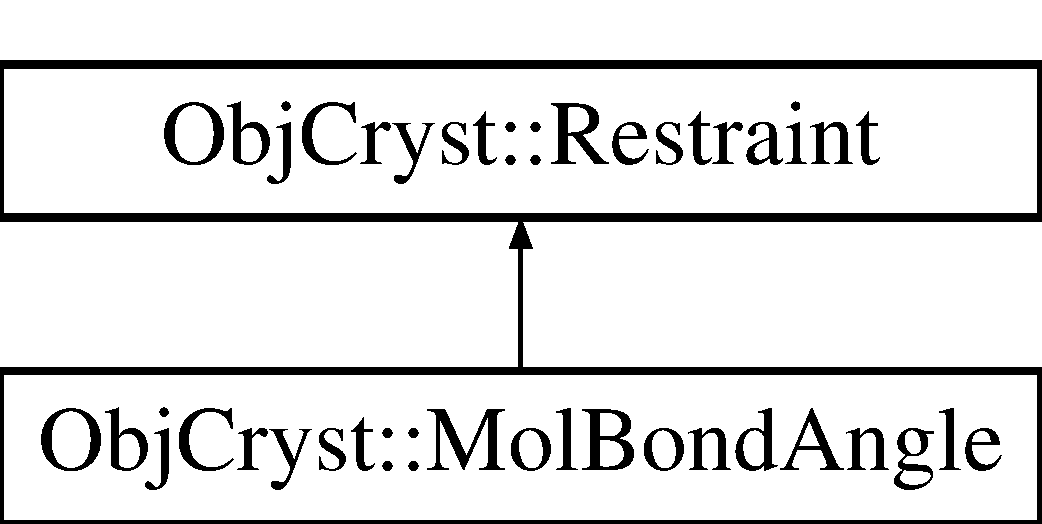
\includegraphics[height=2.000000cm]{a00044}
\end{center}
\end{figure}
\subsubsection*{Public Member Functions}
\begin{DoxyCompactItemize}
\item 
{\bf Mol\-Bond} ({\bf Mol\-Atom} \&atom1, {\bf Mol\-Atom} \&atom2, const R\-E\-A\-L length, const R\-E\-A\-L sigma, const R\-E\-A\-L delta, {\bf Molecule} \&parent, const R\-E\-A\-L bond\-Order=1.)
\begin{DoxyCompactList}\small\item\em Constructor. \end{DoxyCompactList}\item 
virtual {\bf $\sim$\-Mol\-Bond} ()
\begin{DoxyCompactList}\small\item\em Destructor. \end{DoxyCompactList}\item 
const {\bf Molecule} \& {\bfseries Get\-Molecule} () const \label{a00044_a1a3c7684b661b7510938df418dc4b35e}

\item 
{\bf Molecule} \& {\bfseries Get\-Molecule} ()\label{a00044_ad48eecb32e26ec3c3134893b16e9e4b9}

\item 
string {\bf Get\-Name} () const \label{a00044_af085014f7d56f746236d7b131b21c68f}

\begin{DoxyCompactList}\small\item\em Name of the bond, e.\-g. \char`\"{}\-C3-\/\-O4\char`\"{}. \end{DoxyCompactList}\item 
virtual void {\bfseries X\-M\-L\-Output} (ostream \&os, int indent=0) const \label{a00044_a6b0e3c8ae91d926a6e12cc7f5fb6680a}

\item 
virtual void {\bfseries X\-M\-L\-Input} (istream \&is, const {\bf X\-M\-L\-Cryst\-Tag} \&tag)\label{a00044_af655bf9c3ff32e4e972880745ff94a13}

\item 
virtual R\-E\-A\-L {\bf Get\-Log\-Likelihood} () const \label{a00044_af796fe008141e6a6fae7d4049273ccdf}

\begin{DoxyCompactList}\small\item\em Get -\/ln(likelihood) for this restraint. \end{DoxyCompactList}\item 
R\-E\-A\-L {\bfseries Get\-Log\-Likelihood} (const bool calc\-Deriv, const bool recalc) const \label{a00044_ae02e3596ae088d9ae3116e6c3d789899}

\item 
R\-E\-A\-L {\bf Get\-Deriv} (const std\-::map$<$ const {\bf Mol\-Atom} $\ast$, {\bf X\-Y\-Z} $>$ \&m, const bool llk=false) const 
\begin{DoxyCompactList}\small\item\em Get the derivative of the bond length, given the derivatives of the atom positions This requires that Get\-Log\-Likelihood(calc\-Deriv=true) be called first. \end{DoxyCompactList}\item 
void {\bf Calc\-Gradient} (std\-::map$<$ {\bf Mol\-Atom} $\ast$, {\bf X\-Y\-Z} $>$ \&m) const 
\begin{DoxyCompactList}\small\item\em Calc log(likelihood) gradient -\/ versus all atomic coordinates. \end{DoxyCompactList}\item 
const {\bf Mol\-Atom} \& {\bfseries Get\-Atom1} () const \label{a00044_ac55a424209a524004a77a16d08d05e44}

\item 
const {\bf Mol\-Atom} \& {\bfseries Get\-Atom2} () const \label{a00044_a6986775d114461e91a9873d9415cb42f}

\item 
{\bf Mol\-Atom} \& {\bfseries Get\-Atom1} ()\label{a00044_a69a13fd18cb20b2b31c6e71e35e7eb7e}

\item 
{\bf Mol\-Atom} \& {\bfseries Get\-Atom2} ()\label{a00044_a972fe03e0c1b85cdab8ad09ecbd2bd88}

\item 
void {\bfseries Set\-Atom1} ({\bf Mol\-Atom} \&at1)\label{a00044_a134d996eddce994d967b4b3f4358a3dd}

\item 
void {\bfseries Set\-Atom2} ({\bf Mol\-Atom} \&at2)\label{a00044_a6d91f26445b8a4e0ca2c8a4e5af90490}

\item 
R\-E\-A\-L {\bfseries Get\-Length} () const \label{a00044_a16685dcefa38d34d0a92725b000d558f}

\item 
R\-E\-A\-L {\bfseries Get\-Length0} () const \label{a00044_ab6d10bf6342be4ae2f4c58f9d8b5d173}

\item 
R\-E\-A\-L {\bfseries Get\-Length\-Delta} () const \label{a00044_ad5d847da92fe2db752ba45a62f8cdf4a}

\item 
R\-E\-A\-L {\bfseries Get\-Length\-Sigma} () const \label{a00044_aa0837a2385f057bbaa49e1e96bed6399}

\item 
R\-E\-A\-L {\bfseries Get\-Bond\-Order} () const \label{a00044_a778587888f587d23d7d581135b4a99be}

\item 
R\-E\-A\-L \& {\bfseries Length0} ()\label{a00044_a222b10e1cf332cf28220f00c6bab0688}

\item 
R\-E\-A\-L \& {\bfseries Length\-Delta} ()\label{a00044_ad3b78642b705684c5685fc1064e3e051}

\item 
R\-E\-A\-L \& {\bfseries Length\-Sigma} ()\label{a00044_ae8e28507497bccddc50ea678c3a2aa62}

\item 
R\-E\-A\-L \& {\bfseries Bond\-Order} ()\label{a00044_a329946012cb86eee1388b21ec9768ac6}

\item 
void {\bfseries Set\-Length0} (const R\-E\-A\-L length)\label{a00044_a347971edc80f025dca4f7253fea78eb8}

\item 
void {\bfseries Set\-Length\-Delta} (const R\-E\-A\-L length)\label{a00044_a42e9a07e2383dcfdcb5b7f0728be726f}

\item 
void {\bfseries Set\-Length\-Sigma} (const R\-E\-A\-L length)\label{a00044_ab96f037ddc070774b0cb9665e4e1b751}

\item 
void {\bfseries Set\-Bond\-Order} (const R\-E\-A\-L length)\label{a00044_a1050f7fc227c9a925d8f98c01e2e1cc9}

\item 
bool {\bfseries Is\-Free\-Torsion} () const \label{a00044_a95b84b6994623ff1c2f9704ff706b701}

\item 
void {\bfseries Set\-Free\-Torsion} (const bool is\-In\-Ring)\label{a00044_aab0b94a8e27c34d748f4cf7cd0060431}

\end{DoxyCompactItemize}
\subsubsection*{Private Attributes}
\begin{DoxyCompactItemize}
\item 
pair$<$ {\bf Mol\-Atom} $\ast$, {\bf Mol\-Atom} $\ast$ $>$ {\bfseries m\-Atom\-Pair}\label{a00044_ac7cc5382df3fdca08cc9fb17bdfc91d5}

\item 
R\-E\-A\-L {\bfseries m\-Length0}\label{a00044_aa1652cde21c40d1422daf579409b8779}

\item 
R\-E\-A\-L {\bfseries m\-Delta}\label{a00044_ada3df50564e2285ee1f6b659c4dbdee6}

\item 
R\-E\-A\-L {\bfseries m\-Sigma}\label{a00044_a3312763939b3c5f4bcac987b15c1f0b1}

\item 
R\-E\-A\-L {\bfseries m\-Bond\-Order}\label{a00044_a785e2209e844fc83a85c0a20ec9cfe80}

\item 
bool {\bfseries m\-Is\-Free\-Torsion}\label{a00044_ab71a7d1e120f0c351694317e054ec18c}

\item 
{\bf Molecule} $\ast$ {\bf mp\-Mol}\label{a00044_af67c44fd54e60de27f4acb6f2a6e7e3b}

\begin{DoxyCompactList}\small\item\em Parent \doxyref{Molecule}{p.}{a00047}. \end{DoxyCompactList}\item 
R\-E\-A\-L {\bf m\-L\-L\-K}\label{a00044_a48e0a0e15c8d21376732144a43a26264}

\begin{DoxyCompactList}\small\item\em Stored log(likelihood) \end{DoxyCompactList}\item 
{\bf X\-Y\-Z} {\bf m\-Deriv\-Atom1}
\begin{DoxyCompactList}\small\item\em Derivatives of the bond length with respect to the coordinates of the atoms. \end{DoxyCompactList}\item 
{\bf X\-Y\-Z} {\bfseries m\-Deriv\-Atom2}\label{a00044_a692a9986c610412913ddb700b881edc3}

\item 
R\-E\-A\-L {\bf m\-Deriv\-L\-L\-K\-Coeff}
\begin{DoxyCompactList}\small\item\em The factor used to change the derivative of the length/angle, to the derivative of the log(likelihood). \end{DoxyCompactList}\end{DoxyCompactItemize}


\subsubsection{Detailed Description}
Bond between two atoms, also a restraint on the associated bond length. 

\subsubsection{Constructor \& Destructor Documentation}
\index{Obj\-Cryst\-::\-Mol\-Bond@{Obj\-Cryst\-::\-Mol\-Bond}!Mol\-Bond@{Mol\-Bond}}
\index{Mol\-Bond@{Mol\-Bond}!ObjCryst::MolBond@{Obj\-Cryst\-::\-Mol\-Bond}}
\paragraph[{Mol\-Bond}]{\setlength{\rightskip}{0pt plus 5cm}Obj\-Cryst\-::\-Mol\-Bond\-::\-Mol\-Bond (
\begin{DoxyParamCaption}
\item[{{\bf Mol\-Atom} \&}]{atom1, }
\item[{{\bf Mol\-Atom} \&}]{atom2, }
\item[{const R\-E\-A\-L}]{length, }
\item[{const R\-E\-A\-L}]{sigma, }
\item[{const R\-E\-A\-L}]{delta, }
\item[{{\bf Molecule} \&}]{parent, }
\item[{const R\-E\-A\-L}]{bond\-Order = {\ttfamily 1.}}
\end{DoxyParamCaption}
)}\label{a00044_aa5eb1a8ba4e34da2516bfc24af4fabec}


Constructor. 

Both atoms of the bond are told of the creation of the bond, so that they can keep a list of bonds they are involved in.


\begin{DoxyParams}{Parameters}
{\em atom1,atom2,\-:} & the atoms of the bond \\
\hline
{\em length,\-:} & the expected bond length \\
\hline
{\em sigma,delta,\-:} & depending on the calculated length, the log(likelihood) is equal to\-:
\begin{DoxyItemize}
\item within $[length_{0}-\delta;length_{0}+\delta]$\-: $ -\log(likelihood)= \log\left(2\delta+\sqrt{2\pi\sigma^2}\right)$
\item if $length > length_{0}+\delta$\-: $ -\log(likelihood)= \log\left(2\delta+\sqrt{2\pi\sigma^2}\right) + \left(\frac{(length-\delta)-length_{0}}{\sigma} \right)^2$
\item if $length < length_{0}-\delta$\-: $ -\log(likelihood)= \log\left(2\delta+\sqrt{2\pi\sigma^2}\right) + \left(\frac{(length+\delta)-length_{0}}{\sigma} \right)^2$ 
\end{DoxyItemize}\\
\hline
\end{DoxyParams}
\index{Obj\-Cryst\-::\-Mol\-Bond@{Obj\-Cryst\-::\-Mol\-Bond}!$\sim$\-Mol\-Bond@{$\sim$\-Mol\-Bond}}
\index{$\sim$\-Mol\-Bond@{$\sim$\-Mol\-Bond}!ObjCryst::MolBond@{Obj\-Cryst\-::\-Mol\-Bond}}
\paragraph[{$\sim$\-Mol\-Bond}]{\setlength{\rightskip}{0pt plus 5cm}virtual Obj\-Cryst\-::\-Mol\-Bond\-::$\sim$\-Mol\-Bond (
\begin{DoxyParamCaption}
{}
\end{DoxyParamCaption}
)\hspace{0.3cm}{\ttfamily [virtual]}}\label{a00044_a0aac13259fa1079e181d4a04c7556f3e}


Destructor. 

Notifies the atoms that the bond has disappeared. 

\subsubsection{Member Function Documentation}
\index{Obj\-Cryst\-::\-Mol\-Bond@{Obj\-Cryst\-::\-Mol\-Bond}!Calc\-Gradient@{Calc\-Gradient}}
\index{Calc\-Gradient@{Calc\-Gradient}!ObjCryst::MolBond@{Obj\-Cryst\-::\-Mol\-Bond}}
\paragraph[{Calc\-Gradient}]{\setlength{\rightskip}{0pt plus 5cm}void Obj\-Cryst\-::\-Mol\-Bond\-::\-Calc\-Gradient (
\begin{DoxyParamCaption}
\item[{std\-::map$<$ {\bf Mol\-Atom} $\ast$, {\bf X\-Y\-Z} $>$ \&}]{m}
\end{DoxyParamCaption}
) const}\label{a00044_a187126a2a21c5944b2e351fc331fd5c9}


Calc log(likelihood) gradient -\/ versus all atomic coordinates. 


\begin{DoxyParams}{Parameters}
{\em m,\-:} & this map should have been initialized by adding all possible atom pointers as keys, with all \doxyref{X\-Y\-Z}{p.}{a00152} values equal to zeros. On return, the derivative of the log(likelihood) vs each atomic coordinates will {\bfseries added} to each coordinate of the corresponding atoms. \\
\hline
\end{DoxyParams}
\index{Obj\-Cryst\-::\-Mol\-Bond@{Obj\-Cryst\-::\-Mol\-Bond}!Get\-Deriv@{Get\-Deriv}}
\index{Get\-Deriv@{Get\-Deriv}!ObjCryst::MolBond@{Obj\-Cryst\-::\-Mol\-Bond}}
\paragraph[{Get\-Deriv}]{\setlength{\rightskip}{0pt plus 5cm}R\-E\-A\-L Obj\-Cryst\-::\-Mol\-Bond\-::\-Get\-Deriv (
\begin{DoxyParamCaption}
\item[{const std\-::map$<$ const {\bf Mol\-Atom} $\ast$, {\bf X\-Y\-Z} $>$ \&}]{m, }
\item[{const bool}]{llk = {\ttfamily false}}
\end{DoxyParamCaption}
) const}\label{a00044_adeeda31a2485f2985a1a7023cfe374f8}


Get the derivative of the bond length, given the derivatives of the atom positions This requires that Get\-Log\-Likelihood(calc\-Deriv=true) be called first. 

If llk=true, this will return the derivative of the llk rather than the derivative of the length or angle 

\subsubsection{Member Data Documentation}
\index{Obj\-Cryst\-::\-Mol\-Bond@{Obj\-Cryst\-::\-Mol\-Bond}!m\-Deriv\-Atom1@{m\-Deriv\-Atom1}}
\index{m\-Deriv\-Atom1@{m\-Deriv\-Atom1}!ObjCryst::MolBond@{Obj\-Cryst\-::\-Mol\-Bond}}
\paragraph[{m\-Deriv\-Atom1}]{\setlength{\rightskip}{0pt plus 5cm}{\bf X\-Y\-Z} Obj\-Cryst\-::\-Mol\-Bond\-::m\-Deriv\-Atom1\hspace{0.3cm}{\ttfamily [mutable]}, {\ttfamily [private]}}\label{a00044_afbabaca2a8c529a5ed48b86b90b6c7a7}


Derivatives of the bond length with respect to the coordinates of the atoms. 

The derivatives are calculated in Mol\-Bond\-::\-Get\-Log\-Likelihood(true) \index{Obj\-Cryst\-::\-Mol\-Bond@{Obj\-Cryst\-::\-Mol\-Bond}!m\-Deriv\-L\-L\-K\-Coeff@{m\-Deriv\-L\-L\-K\-Coeff}}
\index{m\-Deriv\-L\-L\-K\-Coeff@{m\-Deriv\-L\-L\-K\-Coeff}!ObjCryst::MolBond@{Obj\-Cryst\-::\-Mol\-Bond}}
\paragraph[{m\-Deriv\-L\-L\-K\-Coeff}]{\setlength{\rightskip}{0pt plus 5cm}R\-E\-A\-L Obj\-Cryst\-::\-Mol\-Bond\-::m\-Deriv\-L\-L\-K\-Coeff\hspace{0.3cm}{\ttfamily [mutable]}, {\ttfamily [private]}}\label{a00044_af7ec58bb24811ae897e8ba1ecc33d4de}


The factor used to change the derivative of the length/angle, to the derivative of the log(likelihood). 

e.\-g. (for m\-Delta=0) $ mDerivLLKCoeff = \frac{L-L_0}{\sigma^2} $ 

The documentation for this class was generated from the following file\-:\begin{DoxyCompactItemize}
\item 
Molecule.\-h\end{DoxyCompactItemize}

\subsection{Obj\+Cryst\+:\+:L\+S\+Q\+Num\+Obj Class Reference}
\label{a00045}\index{Obj\+Cryst\+::\+L\+S\+Q\+Num\+Obj@{Obj\+Cryst\+::\+L\+S\+Q\+Num\+Obj}}


(Quick \& dirty) Least-\/\+Squares Refinement Object with Numerical derivatives  


\subsubsection*{Public Member Functions}
\begin{DoxyCompactItemize}
\item 
{\bfseries L\+S\+Q\+Num\+Obj} (std\+::string obj\+Name=\char`\"{}Unnamed L\+S\+Q object\char`\"{})\label{a00045_a2ccb9fe18f1324eef38c6d24740bdf9b}

\item 
const string \& {\bf Get\+Class\+Name} () const \label{a00045_acbad850460a8c8634e64159497805639}

\begin{DoxyCompactList}\small\item\em Name for this class (\char`\"{}\+Refinable\+Obj\char`\"{}, \char`\"{}\+Crystal\char`\"{},...) \end{DoxyCompactList}\item 
const string \& {\bf Get\+Name} () const \label{a00045_a19a33796efc622243e2ca614903f9da1}

\begin{DoxyCompactList}\small\item\em Name of the object. \end{DoxyCompactList}\item 
void {\bf Set\+Par\+Is\+Fixed} (const std\+::string \&par\+Name, const bool fix)
\begin{DoxyCompactList}\small\item\em Fix one parameter. \end{DoxyCompactList}\item 
void {\bf Set\+Par\+Is\+Fixed} (const {\bf Ref\+Par\+Type} $\ast$type, const bool fix)
\begin{DoxyCompactList}\small\item\em Fix one family of parameters. \end{DoxyCompactList}\item 
void {\bf Set\+Par\+Is\+Fixed} ({\bf Refinable\+Par} \&par, const bool fix)
\begin{DoxyCompactList}\small\item\em Fix one parameter. \end{DoxyCompactList}\item 
void {\bf Set\+Par\+Is\+Fixed} ({\bf Refinable\+Obj} \&obj, const bool fix)
\begin{DoxyCompactList}\small\item\em Fix all parameters within an object. \end{DoxyCompactList}\item 
void {\bf Un\+Fix\+All\+Par} ()
\begin{DoxyCompactList}\small\item\em Un\+Fix All parameters. \end{DoxyCompactList}\item 
void {\bf Set\+Par\+Is\+Used} (const std\+::string \&par\+Name, const bool use)
\begin{DoxyCompactList}\small\item\em Set a parameter to be used. \end{DoxyCompactList}\item 
void {\bf Set\+Par\+Is\+Used} (const {\bf Ref\+Par\+Type} $\ast$type, const bool use)
\begin{DoxyCompactList}\small\item\em Set a family of parameters to be used. \end{DoxyCompactList}\item 
void {\bf Refine} (int nb\+Cycle=1, bool use\+Levenberg\+Marquardt=false, const bool silent=false, const bool call\+Begin\+End\+Optimization=true, const float min\+Chi2var=0.\+01)
\begin{DoxyCompactList}\small\item\em Do the refinement. \end{DoxyCompactList}\item 
void {\bf Stop\+After\+Cycle} ()\label{a00045_a4d3d47163ee85c7026901b4a82d512de}

\begin{DoxyCompactList}\small\item\em Stop after the current cycle. Used for refinement interruption. \end{DoxyCompactList}\item 
Cryst\+Vector\+\_\+\+R\+E\+A\+L {\bfseries Sigma} () const \label{a00045_abd95a807a80ea2eaf9e1a724cfdd413e}

\item 
Cryst\+Matrix\+\_\+\+R\+E\+A\+L {\bfseries Correl\+Matrix} () const \label{a00045_a3a1da618157efff1ea1aef46e8f1b524}

\item 
R\+E\+A\+L {\bfseries Rfactor} () const \label{a00045_ae1ad8ab2dd7502a18b8761684983e7ac}

\item 
R\+E\+A\+L {\bfseries Rw\+Factor} () const \label{a00045_ae748ee51f6c3730bc62e7b164fa871c6}

\item 
R\+E\+A\+L {\bfseries Chi\+Square} () const \label{a00045_a89bc494e4fb96b1873e77aec8505f6e3}

\item 
void {\bf Set\+Refined\+Obj} ({\bf Refinable\+Obj} \&obj, const unsigned int L\+S\+Q\+Func\+Index=0, const bool init=true, const bool recursive=false)
\begin{DoxyCompactList}\small\item\em Choose the object to refine. \end{DoxyCompactList}\item 
const std\+::vector$<$ std\+::pair\\*
$<$ {\bf Refinable\+Obj} $\ast$, unsigned int $>$ $>$ \& {\bf Get\+Refined\+Obj\+Map} () const 
\begin{DoxyCompactList}\small\item\em Get the map of refined objects -\/ this is a recursive list of all the objects that are taken into account for the refinement. \end{DoxyCompactList}\item 
std\+::vector$<$ std\+::pair\\*
$<$ {\bf Refinable\+Obj} $\ast$, unsigned int $>$ $>$ \& {\bf Get\+Refined\+Obj\+Map} ()
\begin{DoxyCompactList}\small\item\em Get the map of refined objects -\/ this is a recursive list of all the objects that are taken into account for the refinement. \end{DoxyCompactList}\item 
{\bf Refinable\+Obj} \& {\bf Get\+Compiled\+Refined\+Obj} ()
\begin{DoxyCompactList}\small\item\em Access to the \doxyref{Refinable\+Obj}{p.}{a00077} which is the compilation of all parameters from the object supplied for optimization and its sub-\/objects. \end{DoxyCompactList}\item 
const {\bf Refinable\+Obj} \& {\bf Get\+Compiled\+Refined\+Obj} () const 
\begin{DoxyCompactList}\small\item\em Access to the \doxyref{Refinable\+Obj}{p.}{a00077} which is the compilation of all parameters from the object supplied for optimization and its sub-\/objects. \end{DoxyCompactList}\item 
void {\bfseries Set\+Use\+Save\+File\+On\+Each\+Cycle} (bool yes\+Or\+No=true)\label{a00045_a5052fda0d9764bf06f985ec9443fa145}

\item 
void {\bfseries Set\+Save\+File} (std\+::string file\+Name=\char`\"{}refine.\+save\char`\"{})\label{a00045_a62fe3d8067ee765448a0042a9a34bf2f}

\item 
void {\bfseries Print\+Ref\+Results} () const \label{a00045_a6293e921d940022fe523e85d0c70eea8}

\item 
void {\bfseries Set\+Damping\+Factor} (const R\+E\+A\+L new\+Damp\+Fact)\label{a00045_a0eb066c4614a884d6da923c575d31132}

\item 
void {\bfseries Purge\+Save\+File} ()\label{a00045_ab91c3db60b9ce7de78a39191436878ae}

\item 
void {\bfseries Write\+Report\+To\+File} () const \label{a00045_aadeaa4e66c0772b7b39d7769f5c9ab35}

\item 
void {\bfseries Optimize\+Derivative\+Steps} ()\label{a00045_a29f4c2161390356d75ca1caec508a263}

\item 
const std\+::map$<$ pair$<$ const \\*
{\bf Refinable\+Par} $\ast$, const \\*
{\bf Refinable\+Par} $\ast$ $>$, R\+E\+A\+L $>$ \& {\bfseries Get\+Variance\+Covariance\+Map} () const \label{a00045_a4523a9a61433f2e362bc5a8f17f0de11}

\item 
void {\bf Prepare\+Ref\+Par\+List} (const bool copy\+\_\+param=false)
\begin{DoxyCompactList}\small\item\em Prepare the full parameter list for the refinement. \end{DoxyCompactList}\item 
const Cryst\+Vector\+\_\+\+R\+E\+A\+L \& {\bf Get\+L\+S\+Q\+Calc} () const \label{a00045_ab6c69bdc3cffebda96e7f8da2a10651b}

\begin{DoxyCompactList}\small\item\em Get the L\+S\+Q calc vector (using either only the top or the hierarchy of object) \end{DoxyCompactList}\item 
const Cryst\+Vector\+\_\+\+R\+E\+A\+L \& {\bf Get\+L\+S\+Q\+Obs} () const \label{a00045_a9ae138310620a13651dfbee5faf8b7d3}

\begin{DoxyCompactList}\small\item\em Get the L\+S\+Q obs vector (using either only the top or the hierarchy of object) \end{DoxyCompactList}\item 
const Cryst\+Vector\+\_\+\+R\+E\+A\+L \& {\bf Get\+L\+S\+Q\+Weight} () const \label{a00045_a448b1e7bcaea617b6c3b0f58540a1d5c}

\begin{DoxyCompactList}\small\item\em Get the L\+S\+Q weight vector (using either only the top or the hierarchy of object) \end{DoxyCompactList}\item 
const Cryst\+Vector\+\_\+\+R\+E\+A\+L \& {\bf Get\+L\+S\+Q\+Deriv} ({\bf Refinable\+Par} \&par)\label{a00045_add2acd529c8c8c4dc38f1d09f7b637ce}

\begin{DoxyCompactList}\small\item\em Get the L\+S\+Q deriv vector (using either only the top or the hierarchy of object) \end{DoxyCompactList}\item 
void {\bf Begin\+Optimization} (const bool allow\+Approximations=false, const bool enable\+Restraints=false)\label{a00045_a6230c952ec8fc2c0ed63ac1b4de232a5}

\begin{DoxyCompactList}\small\item\em Tell all refined object that the refinement is beginning. \end{DoxyCompactList}\item 
void {\bf End\+Optimization} ()\label{a00045_a4c6168e319fd4a8f949997d1b54012ba}

\begin{DoxyCompactList}\small\item\em Tell all refined object that the refinement is finished. \end{DoxyCompactList}\end{DoxyCompactItemize}
\subsubsection*{Private Attributes}
\begin{DoxyCompactItemize}
\item 
{\bf Obj\+Registry}$<$ {\bf Refinable\+Obj} $>$ {\bf m\+Recursive\+Refined\+Obj\+List}\label{a00045_a23d277120b16313b7d65ba43474c8bb2}

\begin{DoxyCompactList}\small\item\em The recursive list of all refined sub-\/objects. \end{DoxyCompactList}\item 
{\bf Refinable\+Obj} {\bf m\+Ref\+Par\+List}
\begin{DoxyCompactList}\small\item\em The refinable par list used during refinement. \end{DoxyCompactList}\item 
R\+E\+A\+L {\bf m\+Damping\+Factor}\label{a00045_aba399e82e28a4cfe9e69aefc797f04cf}

\begin{DoxyCompactList}\small\item\em Damping factor for the refinement (unused yet...) \end{DoxyCompactList}\item 
bool {\bf m\+Save\+Report\+On\+Each\+Cycle}\label{a00045_a09babc65e743bac7f89f86fc08d59899}

\begin{DoxyCompactList}\small\item\em Save result to file after each cycle ? \end{DoxyCompactList}\item 
std\+::string {\bf m\+Name}\label{a00045_a72b3294b9fa16e5fc0d58bebaf6afb7c}

\begin{DoxyCompactList}\small\item\em Name of the refined object. \end{DoxyCompactList}\item 
std\+::string {\bf m\+Save\+File\+Name}\label{a00045_abe4fdfa21b103fa7c43dbc643c303bbf}

\begin{DoxyCompactList}\small\item\em File name where refinement info is saved. \end{DoxyCompactList}\item 
R\+E\+A\+L {\bfseries m\+R}\label{a00045_a81e6e3477ce61e5ba4aa9087c18423e7}

\item 
R\+E\+A\+L {\bfseries m\+Rw}\label{a00045_ab0ebd8803606b2666d402b7ced3d3bc4}

\item 
R\+E\+A\+L {\bfseries m\+Chi\+Sq}\label{a00045_ab1a1232379bae302dcb217d6e359e7dc}

\item 
R\+E\+A\+L {\bfseries m\+Rex}\label{a00045_a7781827b6f8cb60142c041952f99a6c5}

\item 
Cryst\+Matrix\+\_\+\+R\+E\+A\+L {\bf m\+Correl\+Matrix}\label{a00045_a85feb318b2d5804324b55e1e3aa65fbf}

\begin{DoxyCompactList}\small\item\em Correlation matrix between all refined parameters. \end{DoxyCompactList}\item 
std\+::map$<$ pair$<$ const \\*
{\bf Refinable\+Par} $\ast$, const \\*
{\bf Refinable\+Par} $\ast$ $>$, R\+E\+A\+L $>$ {\bf mv\+Var\+Covar}\label{a00045_a680f9ab902de1ccfd34061131a1399b5}

\begin{DoxyCompactList}\small\item\em Variance-\/\+Covariance matrix, as a std\+::map. \end{DoxyCompactList}\item 
Cryst\+Vector\+\_\+\+R\+E\+A\+L {\bf m\+Obs}\label{a00045_aaf6851846648464a65902618a5c37c09}

\begin{DoxyCompactList}\small\item\em Observed values. \end{DoxyCompactList}\item 
Cryst\+Vector\+\_\+\+R\+E\+A\+L {\bf m\+Weight}\label{a00045_af15db099da89847aed6a5106d2c68279}

\begin{DoxyCompactList}\small\item\em Weight corresponding to all observed values. \end{DoxyCompactList}\item 
int {\bf m\+Index\+Values\+Set\+Initial}
\begin{DoxyCompactList}\small\item\em Index of the set of saved values for all refinable parameters, before refinement and before the last cycle. \end{DoxyCompactList}\item 
int {\bfseries m\+Index\+Values\+Set\+Last}\label{a00045_a52651e7d92c699c8a282c2eef065055d}

\item 
bool {\bf m\+Stop\+After\+Cycle}\label{a00045_aa33d466b132ac98408619cbe230871ce}

\begin{DoxyCompactList}\small\item\em If true, then stop at the end of the cycle. Used in multi-\/threading environment. \end{DoxyCompactList}\item 
std\+::vector$<$ std\+::pair\\*
$<$ {\bf Refinable\+Obj} $\ast$, unsigned int $>$ $>$ {\bf mv\+Refined\+Obj\+Map}
\begin{DoxyCompactList}\small\item\em Map of the recursive list of the objects to be refined. \end{DoxyCompactList}\item 
bool {\bf m\+Copy\+Ref\+Par}
\begin{DoxyCompactList}\small\item\em If true, then parameters to be refined will be copied instead of referenced. \end{DoxyCompactList}\item 
Cryst\+Vector\+\_\+\+R\+E\+A\+L {\bf m\+L\+S\+Q\+Obs}\label{a00045_a0209969eff2d3db1175246f6321f8e0c}

\begin{DoxyCompactList}\small\item\em Temporary arrays for L\+S\+Q functions evaluation -\/ used when using recursive L\+S\+Q function. \end{DoxyCompactList}\item 
Cryst\+Vector\+\_\+\+R\+E\+A\+L {\bfseries m\+L\+S\+Q\+Calc}\label{a00045_a99ea1b948bb832d5f962c957d2002663}

\item 
Cryst\+Vector\+\_\+\+R\+E\+A\+L {\bfseries m\+L\+S\+Q\+Weight}\label{a00045_a7f40708d08b3f87ef35c0c652c8047cc}

\item 
Cryst\+Vector\+\_\+\+R\+E\+A\+L {\bfseries m\+L\+S\+Q\+Deriv}\label{a00045_a36367b2655942c2dd718e5bab2f1174f}

\end{DoxyCompactItemize}


\subsubsection{Detailed Description}
(Quick \& dirty) Least-\/\+Squares Refinement Object with Numerical derivatives 

This is still highly experimental ! 

\subsubsection{Member Function Documentation}
\index{Obj\+Cryst\+::\+L\+S\+Q\+Num\+Obj@{Obj\+Cryst\+::\+L\+S\+Q\+Num\+Obj}!Get\+Compiled\+Refined\+Obj@{Get\+Compiled\+Refined\+Obj}}
\index{Get\+Compiled\+Refined\+Obj@{Get\+Compiled\+Refined\+Obj}!Obj\+Cryst\+::\+L\+S\+Q\+Num\+Obj@{Obj\+Cryst\+::\+L\+S\+Q\+Num\+Obj}}
\paragraph[{Get\+Compiled\+Refined\+Obj}]{\setlength{\rightskip}{0pt plus 5cm}{\bf Refinable\+Obj}\& Obj\+Cryst\+::\+L\+S\+Q\+Num\+Obj\+::\+Get\+Compiled\+Refined\+Obj (
\begin{DoxyParamCaption}
{}
\end{DoxyParamCaption}
)}\label{a00045_af9f5ae207a1ee7d9574a3493577a9108}


Access to the \doxyref{Refinable\+Obj}{p.}{a00077} which is the compilation of all parameters from the object supplied for optimization and its sub-\/objects. 

Since this compilation is only updated from the suplied refinableobj and its sub-\/objects when \doxyref{Set\+Refined\+Obj()}{p.}{a00045_ac093bab1bcb43aa4ea00f63fdb53063f} and \doxyref{Prepare\+Ref\+Par\+List()}{p.}{a00045_afdeb58450a3e0506fc02a0b5df15a600} are called, it is possible to alter the fixed/limited status of parameters here without affecting the parameters in the refined objects. \index{Obj\+Cryst\+::\+L\+S\+Q\+Num\+Obj@{Obj\+Cryst\+::\+L\+S\+Q\+Num\+Obj}!Get\+Compiled\+Refined\+Obj@{Get\+Compiled\+Refined\+Obj}}
\index{Get\+Compiled\+Refined\+Obj@{Get\+Compiled\+Refined\+Obj}!Obj\+Cryst\+::\+L\+S\+Q\+Num\+Obj@{Obj\+Cryst\+::\+L\+S\+Q\+Num\+Obj}}
\paragraph[{Get\+Compiled\+Refined\+Obj}]{\setlength{\rightskip}{0pt plus 5cm}const {\bf Refinable\+Obj}\& Obj\+Cryst\+::\+L\+S\+Q\+Num\+Obj\+::\+Get\+Compiled\+Refined\+Obj (
\begin{DoxyParamCaption}
{}
\end{DoxyParamCaption}
) const}\label{a00045_af94ebfd178b0c689130f8f99c2bd11da}


Access to the \doxyref{Refinable\+Obj}{p.}{a00077} which is the compilation of all parameters from the object supplied for optimization and its sub-\/objects. 

Since this compilation is only updated from the suplied refinableobj and its sub-\/objects when \doxyref{Set\+Refined\+Obj()}{p.}{a00045_ac093bab1bcb43aa4ea00f63fdb53063f} and \doxyref{Prepare\+Ref\+Par\+List()}{p.}{a00045_afdeb58450a3e0506fc02a0b5df15a600} are called, it is possible to alter the fixed/limited status of parameters here without affecting the parameters in the refined objects. \index{Obj\+Cryst\+::\+L\+S\+Q\+Num\+Obj@{Obj\+Cryst\+::\+L\+S\+Q\+Num\+Obj}!Get\+Refined\+Obj\+Map@{Get\+Refined\+Obj\+Map}}
\index{Get\+Refined\+Obj\+Map@{Get\+Refined\+Obj\+Map}!Obj\+Cryst\+::\+L\+S\+Q\+Num\+Obj@{Obj\+Cryst\+::\+L\+S\+Q\+Num\+Obj}}
\paragraph[{Get\+Refined\+Obj\+Map}]{\setlength{\rightskip}{0pt plus 5cm}const std\+::vector$<$ std\+::pair$<${\bf Refinable\+Obj}$\ast$,unsigned int$>$ $>$\& Obj\+Cryst\+::\+L\+S\+Q\+Num\+Obj\+::\+Get\+Refined\+Obj\+Map (
\begin{DoxyParamCaption}
{}
\end{DoxyParamCaption}
) const}\label{a00045_a9465c139a524e2ee6890ca43eaf6570e}


Get the map of refined objects -\/ this is a recursive list of all the objects that are taken into account for the refinement. 

The key is a pointer to the object and the value is the L\+S\+Q function index for that object. \index{Obj\+Cryst\+::\+L\+S\+Q\+Num\+Obj@{Obj\+Cryst\+::\+L\+S\+Q\+Num\+Obj}!Get\+Refined\+Obj\+Map@{Get\+Refined\+Obj\+Map}}
\index{Get\+Refined\+Obj\+Map@{Get\+Refined\+Obj\+Map}!Obj\+Cryst\+::\+L\+S\+Q\+Num\+Obj@{Obj\+Cryst\+::\+L\+S\+Q\+Num\+Obj}}
\paragraph[{Get\+Refined\+Obj\+Map}]{\setlength{\rightskip}{0pt plus 5cm}std\+::vector$<$ std\+::pair$<${\bf Refinable\+Obj}$\ast$,unsigned int$>$ $>$\& Obj\+Cryst\+::\+L\+S\+Q\+Num\+Obj\+::\+Get\+Refined\+Obj\+Map (
\begin{DoxyParamCaption}
{}
\end{DoxyParamCaption}
)}\label{a00045_a8126e070d6d5efe7866b5f686e8efb40}


Get the map of refined objects -\/ this is a recursive list of all the objects that are taken into account for the refinement. 

The key is a pointer to the object and the value is the L\+S\+Q function index for that object. \index{Obj\+Cryst\+::\+L\+S\+Q\+Num\+Obj@{Obj\+Cryst\+::\+L\+S\+Q\+Num\+Obj}!Prepare\+Ref\+Par\+List@{Prepare\+Ref\+Par\+List}}
\index{Prepare\+Ref\+Par\+List@{Prepare\+Ref\+Par\+List}!Obj\+Cryst\+::\+L\+S\+Q\+Num\+Obj@{Obj\+Cryst\+::\+L\+S\+Q\+Num\+Obj}}
\paragraph[{Prepare\+Ref\+Par\+List}]{\setlength{\rightskip}{0pt plus 5cm}void Obj\+Cryst\+::\+L\+S\+Q\+Num\+Obj\+::\+Prepare\+Ref\+Par\+List (
\begin{DoxyParamCaption}
\item[{const bool}]{copy\+\_\+param = {\ttfamily false}}
\end{DoxyParamCaption}
)}\label{a00045_afdeb58450a3e0506fc02a0b5df15a600}


Prepare the full parameter list for the refinement. 


\begin{DoxyParams}{Parameters}
{\em copy\+\_\+param} & if false (the default), then the lsq algorithm will work directly on the parameters of the refined object and sub-\/object. So that any modification to the fixed/used/limited status applies permanently to the parameters. if true, then the parameters are copied and therefore only the value of the parameter is changed (and the clocks are ticked).\\
\hline
\end{DoxyParams}
\begin{DoxyNote}{Note}
\+: if copy\+\_\+param==true, then any modification to the parameters (fixed, limited, used status) only affects the copy and not the original. Also, calling again Prepare\+Ref\+Par\+List cancels any such modification.

This will be called automatically before starting the refinement only if the parameter list is empty. Otherwise it should be called before refinement. 
\end{DoxyNote}
\index{Obj\+Cryst\+::\+L\+S\+Q\+Num\+Obj@{Obj\+Cryst\+::\+L\+S\+Q\+Num\+Obj}!Refine@{Refine}}
\index{Refine@{Refine}!Obj\+Cryst\+::\+L\+S\+Q\+Num\+Obj@{Obj\+Cryst\+::\+L\+S\+Q\+Num\+Obj}}
\paragraph[{Refine}]{\setlength{\rightskip}{0pt plus 5cm}void Obj\+Cryst\+::\+L\+S\+Q\+Num\+Obj\+::\+Refine (
\begin{DoxyParamCaption}
\item[{int}]{nb\+Cycle = {\ttfamily 1}, }
\item[{bool}]{use\+Levenberg\+Marquardt = {\ttfamily false}, }
\item[{const bool}]{silent = {\ttfamily false}, }
\item[{const bool}]{call\+Begin\+End\+Optimization = {\ttfamily true}, }
\item[{const float}]{min\+Chi2var = {\ttfamily 0.01}}
\end{DoxyParamCaption}
)}\label{a00045_aaf5ceefe54c4fdfd0e48c3f5cd4f66b9}


Do the refinement. 


\begin{DoxyParams}{Parameters}
{\em nb\+Cycle} & number of L\+S\+Q cycles -\/ if negative, the algorithm will continue until it reaches (-\/nbcycle) or until the relative variation in Chi2 is less than min\+Chi2var \\
\hline
{\em use\+Levenberg\+Marquardt} & enable Levenberg-\/\+Marquardt algorithm to ensure that a decrease of Chi$^\wedge$2 will be obtained (actually a 1\% increase is allowed) \\
\hline
{\em call\+Begin\+End\+Optimization} & if true, will call \doxyref{Refinable\+Obj\+::\+Begin\+Optimization}{p.}{a00077_ababd8f2916e41a20d2c1b21f6ffefe96}(true,...) and \doxyref{Refinable\+Obj\+::\+End\+Optimization()}{p.}{a00077_ab0035f6164cb24ace67b51b11993a851}. You may not want this if the L\+S\+Q is done during another (e.\+g. monte-\/carlo) optimization -\/ but then the calling function {\bfseries must} ensure that approximations are disabled (using \doxyref{Refinable\+Obj\+::\+Set\+Approximation\+Flag}{p.}{a00077_a565c41c23c04f5945512374ae671e2e3}) for objects where that would render derivative calculations imprecise. \\
\hline
{\em min\+Chi2var} & used for termination of the refinement if the relative variation of Chi2 between two successive cyles is less than min\+Chi2var \\
\hline
\end{DoxyParams}
\index{Obj\+Cryst\+::\+L\+S\+Q\+Num\+Obj@{Obj\+Cryst\+::\+L\+S\+Q\+Num\+Obj}!Set\+Par\+Is\+Fixed@{Set\+Par\+Is\+Fixed}}
\index{Set\+Par\+Is\+Fixed@{Set\+Par\+Is\+Fixed}!Obj\+Cryst\+::\+L\+S\+Q\+Num\+Obj@{Obj\+Cryst\+::\+L\+S\+Q\+Num\+Obj}}
\paragraph[{Set\+Par\+Is\+Fixed}]{\setlength{\rightskip}{0pt plus 5cm}void Obj\+Cryst\+::\+L\+S\+Q\+Num\+Obj\+::\+Set\+Par\+Is\+Fixed (
\begin{DoxyParamCaption}
\item[{const std\+::string \&}]{par\+Name, }
\item[{const bool}]{fix}
\end{DoxyParamCaption}
)}\label{a00045_a0bc210b1f4e4b7099493d71c1a7c084d}


Fix one parameter. 

\doxyref{L\+S\+Q\+Num\+Obj\+::\+Prepare\+Ref\+Par\+List()}{p.}{a00045_afdeb58450a3e0506fc02a0b5df15a600} must be called first! \index{Obj\+Cryst\+::\+L\+S\+Q\+Num\+Obj@{Obj\+Cryst\+::\+L\+S\+Q\+Num\+Obj}!Set\+Par\+Is\+Fixed@{Set\+Par\+Is\+Fixed}}
\index{Set\+Par\+Is\+Fixed@{Set\+Par\+Is\+Fixed}!Obj\+Cryst\+::\+L\+S\+Q\+Num\+Obj@{Obj\+Cryst\+::\+L\+S\+Q\+Num\+Obj}}
\paragraph[{Set\+Par\+Is\+Fixed}]{\setlength{\rightskip}{0pt plus 5cm}void Obj\+Cryst\+::\+L\+S\+Q\+Num\+Obj\+::\+Set\+Par\+Is\+Fixed (
\begin{DoxyParamCaption}
\item[{const {\bf Ref\+Par\+Type} $\ast$}]{type, }
\item[{const bool}]{fix}
\end{DoxyParamCaption}
)}\label{a00045_a1be81668c496a3232e4b8416a3414bf3}


Fix one family of parameters. 

\doxyref{L\+S\+Q\+Num\+Obj\+::\+Prepare\+Ref\+Par\+List()}{p.}{a00045_afdeb58450a3e0506fc02a0b5df15a600} must be called first! \index{Obj\+Cryst\+::\+L\+S\+Q\+Num\+Obj@{Obj\+Cryst\+::\+L\+S\+Q\+Num\+Obj}!Set\+Par\+Is\+Fixed@{Set\+Par\+Is\+Fixed}}
\index{Set\+Par\+Is\+Fixed@{Set\+Par\+Is\+Fixed}!Obj\+Cryst\+::\+L\+S\+Q\+Num\+Obj@{Obj\+Cryst\+::\+L\+S\+Q\+Num\+Obj}}
\paragraph[{Set\+Par\+Is\+Fixed}]{\setlength{\rightskip}{0pt plus 5cm}void Obj\+Cryst\+::\+L\+S\+Q\+Num\+Obj\+::\+Set\+Par\+Is\+Fixed (
\begin{DoxyParamCaption}
\item[{{\bf Refinable\+Par} \&}]{par, }
\item[{const bool}]{fix}
\end{DoxyParamCaption}
)}\label{a00045_ad240667179e473c6c16e8928893dfdf8}


Fix one parameter. 

Note that this will fix the copied parameter, not the one in the original object. The supplied \doxyref{Refinable\+Par}{p.}{a00079} may be either the copied one or the original.

\doxyref{L\+S\+Q\+Num\+Obj\+::\+Prepare\+Ref\+Par\+List()}{p.}{a00045_afdeb58450a3e0506fc02a0b5df15a600} must be called first! \index{Obj\+Cryst\+::\+L\+S\+Q\+Num\+Obj@{Obj\+Cryst\+::\+L\+S\+Q\+Num\+Obj}!Set\+Par\+Is\+Fixed@{Set\+Par\+Is\+Fixed}}
\index{Set\+Par\+Is\+Fixed@{Set\+Par\+Is\+Fixed}!Obj\+Cryst\+::\+L\+S\+Q\+Num\+Obj@{Obj\+Cryst\+::\+L\+S\+Q\+Num\+Obj}}
\paragraph[{Set\+Par\+Is\+Fixed}]{\setlength{\rightskip}{0pt plus 5cm}void Obj\+Cryst\+::\+L\+S\+Q\+Num\+Obj\+::\+Set\+Par\+Is\+Fixed (
\begin{DoxyParamCaption}
\item[{{\bf Refinable\+Obj} \&}]{obj, }
\item[{const bool}]{fix}
\end{DoxyParamCaption}
)}\label{a00045_a6fdf2b9d64a527b0c2e81f92fd9be2c3}


Fix all parameters within an object. 

Note that this will fix the copied parameters, not the one in the original objects.

\doxyref{L\+S\+Q\+Num\+Obj\+::\+Prepare\+Ref\+Par\+List()}{p.}{a00045_afdeb58450a3e0506fc02a0b5df15a600} must be called first! \index{Obj\+Cryst\+::\+L\+S\+Q\+Num\+Obj@{Obj\+Cryst\+::\+L\+S\+Q\+Num\+Obj}!Set\+Par\+Is\+Used@{Set\+Par\+Is\+Used}}
\index{Set\+Par\+Is\+Used@{Set\+Par\+Is\+Used}!Obj\+Cryst\+::\+L\+S\+Q\+Num\+Obj@{Obj\+Cryst\+::\+L\+S\+Q\+Num\+Obj}}
\paragraph[{Set\+Par\+Is\+Used}]{\setlength{\rightskip}{0pt plus 5cm}void Obj\+Cryst\+::\+L\+S\+Q\+Num\+Obj\+::\+Set\+Par\+Is\+Used (
\begin{DoxyParamCaption}
\item[{const std\+::string \&}]{par\+Name, }
\item[{const bool}]{use}
\end{DoxyParamCaption}
)}\label{a00045_ab4da8ad96c83cb850145c028e0acb1a7}


Set a parameter to be used. 

\doxyref{L\+S\+Q\+Num\+Obj\+::\+Prepare\+Ref\+Par\+List()}{p.}{a00045_afdeb58450a3e0506fc02a0b5df15a600} must be called first! \index{Obj\+Cryst\+::\+L\+S\+Q\+Num\+Obj@{Obj\+Cryst\+::\+L\+S\+Q\+Num\+Obj}!Set\+Par\+Is\+Used@{Set\+Par\+Is\+Used}}
\index{Set\+Par\+Is\+Used@{Set\+Par\+Is\+Used}!Obj\+Cryst\+::\+L\+S\+Q\+Num\+Obj@{Obj\+Cryst\+::\+L\+S\+Q\+Num\+Obj}}
\paragraph[{Set\+Par\+Is\+Used}]{\setlength{\rightskip}{0pt plus 5cm}void Obj\+Cryst\+::\+L\+S\+Q\+Num\+Obj\+::\+Set\+Par\+Is\+Used (
\begin{DoxyParamCaption}
\item[{const {\bf Ref\+Par\+Type} $\ast$}]{type, }
\item[{const bool}]{use}
\end{DoxyParamCaption}
)}\label{a00045_a3164f80e5cecec4920aa8fae530a4ebe}


Set a family of parameters to be used. 

\doxyref{L\+S\+Q\+Num\+Obj\+::\+Prepare\+Ref\+Par\+List()}{p.}{a00045_afdeb58450a3e0506fc02a0b5df15a600} must be called first! \index{Obj\+Cryst\+::\+L\+S\+Q\+Num\+Obj@{Obj\+Cryst\+::\+L\+S\+Q\+Num\+Obj}!Set\+Refined\+Obj@{Set\+Refined\+Obj}}
\index{Set\+Refined\+Obj@{Set\+Refined\+Obj}!Obj\+Cryst\+::\+L\+S\+Q\+Num\+Obj@{Obj\+Cryst\+::\+L\+S\+Q\+Num\+Obj}}
\paragraph[{Set\+Refined\+Obj}]{\setlength{\rightskip}{0pt plus 5cm}void Obj\+Cryst\+::\+L\+S\+Q\+Num\+Obj\+::\+Set\+Refined\+Obj (
\begin{DoxyParamCaption}
\item[{{\bf Refinable\+Obj} \&}]{obj, }
\item[{const unsigned int}]{L\+S\+Q\+Func\+Index = {\ttfamily 0}, }
\item[{const bool}]{init = {\ttfamily true}, }
\item[{const bool}]{recursive = {\ttfamily false}}
\end{DoxyParamCaption}
)}\label{a00045_ac093bab1bcb43aa4ea00f63fdb53063f}


Choose the object to refine. 

The minimization will be done against its L\+S\+Q function and its parameters, as well as the L\+S\+Q functions and parameters of its sub-\/objects (if recursive==true)


\begin{DoxyParams}{Parameters}
{\em L\+S\+Q\+Func\+Index} & one object can have a choice of several L\+S\+Q functions to minimize-\/ this allows to choose which one to minimize.\\
\hline
{\em init} & if true, the list of refined objects is first cleared. otherwise the new object (and its sub-\/objects) is just added to the list.\\
\hline
{\em recursive} & if false, only the supplied object is added, and not its sub-\/objects \\
\hline
\end{DoxyParams}
\index{Obj\+Cryst\+::\+L\+S\+Q\+Num\+Obj@{Obj\+Cryst\+::\+L\+S\+Q\+Num\+Obj}!Un\+Fix\+All\+Par@{Un\+Fix\+All\+Par}}
\index{Un\+Fix\+All\+Par@{Un\+Fix\+All\+Par}!Obj\+Cryst\+::\+L\+S\+Q\+Num\+Obj@{Obj\+Cryst\+::\+L\+S\+Q\+Num\+Obj}}
\paragraph[{Un\+Fix\+All\+Par}]{\setlength{\rightskip}{0pt plus 5cm}void Obj\+Cryst\+::\+L\+S\+Q\+Num\+Obj\+::\+Un\+Fix\+All\+Par (
\begin{DoxyParamCaption}
{}
\end{DoxyParamCaption}
)}\label{a00045_ad7a98f0a5a88f61ec49ba66f558fe567}


Un\+Fix All parameters. 

\doxyref{L\+S\+Q\+Num\+Obj\+::\+Prepare\+Ref\+Par\+List()}{p.}{a00045_afdeb58450a3e0506fc02a0b5df15a600} must be called first! 

\subsubsection{Member Data Documentation}
\index{Obj\+Cryst\+::\+L\+S\+Q\+Num\+Obj@{Obj\+Cryst\+::\+L\+S\+Q\+Num\+Obj}!m\+Copy\+Ref\+Par@{m\+Copy\+Ref\+Par}}
\index{m\+Copy\+Ref\+Par@{m\+Copy\+Ref\+Par}!Obj\+Cryst\+::\+L\+S\+Q\+Num\+Obj@{Obj\+Cryst\+::\+L\+S\+Q\+Num\+Obj}}
\paragraph[{m\+Copy\+Ref\+Par}]{\setlength{\rightskip}{0pt plus 5cm}bool Obj\+Cryst\+::\+L\+S\+Q\+Num\+Obj\+::m\+Copy\+Ref\+Par\hspace{0.3cm}{\ttfamily [private]}}\label{a00045_a105c818fbabf06c50d930cc5286dabd6}


If true, then parameters to be refined will be copied instead of referenced. 

Therefore only their values and the parameter's clocks are affected when working on the copy. \index{Obj\+Cryst\+::\+L\+S\+Q\+Num\+Obj@{Obj\+Cryst\+::\+L\+S\+Q\+Num\+Obj}!m\+Index\+Values\+Set\+Initial@{m\+Index\+Values\+Set\+Initial}}
\index{m\+Index\+Values\+Set\+Initial@{m\+Index\+Values\+Set\+Initial}!Obj\+Cryst\+::\+L\+S\+Q\+Num\+Obj@{Obj\+Cryst\+::\+L\+S\+Q\+Num\+Obj}}
\paragraph[{m\+Index\+Values\+Set\+Initial}]{\setlength{\rightskip}{0pt plus 5cm}int Obj\+Cryst\+::\+L\+S\+Q\+Num\+Obj\+::m\+Index\+Values\+Set\+Initial\hspace{0.3cm}{\ttfamily [private]}}\label{a00045_afbc070643a325bf40c541689b3f3ef34}


Index of the set of saved values for all refinable parameters, before refinement and before the last cycle. 

\index{Obj\+Cryst\+::\+L\+S\+Q\+Num\+Obj@{Obj\+Cryst\+::\+L\+S\+Q\+Num\+Obj}!m\+Ref\+Par\+List@{m\+Ref\+Par\+List}}
\index{m\+Ref\+Par\+List@{m\+Ref\+Par\+List}!Obj\+Cryst\+::\+L\+S\+Q\+Num\+Obj@{Obj\+Cryst\+::\+L\+S\+Q\+Num\+Obj}}
\paragraph[{m\+Ref\+Par\+List}]{\setlength{\rightskip}{0pt plus 5cm}{\bf Refinable\+Obj} Obj\+Cryst\+::\+L\+S\+Q\+Num\+Obj\+::m\+Ref\+Par\+List\hspace{0.3cm}{\ttfamily [mutable]}, {\ttfamily [private]}}\label{a00045_a81c41272858837f00d21f3db2a3312bb}


The refinable par list used during refinement. 

It is only a compilation of the parameters in \doxyref{Refinable\+Obj}{p.}{a00077} and its sub-\/objects

This list is only updated from the suplied refinableobj and its sub-\/objects when \doxyref{Set\+Refined\+Obj()}{p.}{a00045_ac093bab1bcb43aa4ea00f63fdb53063f} and \doxyref{Prepare\+Ref\+Par\+List()}{p.}{a00045_afdeb58450a3e0506fc02a0b5df15a600} are called, so it is possible to alter the fixed/limited status of parameters here without affecting the parameters in the refined objects. \index{Obj\+Cryst\+::\+L\+S\+Q\+Num\+Obj@{Obj\+Cryst\+::\+L\+S\+Q\+Num\+Obj}!mv\+Refined\+Obj\+Map@{mv\+Refined\+Obj\+Map}}
\index{mv\+Refined\+Obj\+Map@{mv\+Refined\+Obj\+Map}!Obj\+Cryst\+::\+L\+S\+Q\+Num\+Obj@{Obj\+Cryst\+::\+L\+S\+Q\+Num\+Obj}}
\paragraph[{mv\+Refined\+Obj\+Map}]{\setlength{\rightskip}{0pt plus 5cm}std\+::vector$<$ std\+::pair$<${\bf Refinable\+Obj}$\ast$,unsigned int$>$ $>$ Obj\+Cryst\+::\+L\+S\+Q\+Num\+Obj\+::mv\+Refined\+Obj\+Map\hspace{0.3cm}{\ttfamily [private]}}\label{a00045_a910de8d3e6e961ee32a72a445ab4c059}


Map of the recursive list of the objects to be refined. 

The key is the pointer to the object and the value the L\+S\+Q function index

Individual L\+S\+Q functions can be changed using \doxyref{Get\+Refined\+Obj\+Map()}{p.}{a00045_a8126e070d6d5efe7866b5f686e8efb40}. 

The documentation for this class was generated from the following file\+:\begin{DoxyCompactItemize}
\item 
L\+S\+Q\+Num\+Obj.\+h\end{DoxyCompactItemize}

\subsection{Obj\+Cryst\+:\+:L\+S\+Q\+Regularization\+Operator Class Reference}
\label{a00046}\index{Obj\+Cryst\+::\+L\+S\+Q\+Regularization\+Operator@{Obj\+Cryst\+::\+L\+S\+Q\+Regularization\+Operator}}


Simple Regularization Operator for the Least-\/\+Squares Refinement.  


\subsubsection*{Public Member Functions}
\begin{DoxyCompactItemize}
\item 
{\bf L\+S\+Q\+Regularization\+Operator} (std\+::string obj\+Name=\char`\"{}Unnamed L\+S\+Q Regularization Obj\char`\"{})\label{a00046_a8b50ee303228c67b0291497edbec4a4d}

\begin{DoxyCompactList}\small\item\em Constructor. \end{DoxyCompactList}\item 
{\bf L\+S\+Q\+Regularization\+Operator} (const {\bf L\+S\+Q\+Regularization\+Operator} \&)\label{a00046_a3a7df3e9372bd0b5824b3eb46479a479}

\begin{DoxyCompactList}\small\item\em Copy constructor. \end{DoxyCompactList}\item 
{\bf $\sim$\+L\+S\+Q\+Regularization\+Operator} ()\label{a00046_a09d06b5ad20ded0c5361dfac53e79d78}

\begin{DoxyCompactList}\small\item\em Descructor. \end{DoxyCompactList}\item 
const string \& {\bf Get\+Class\+Name} () const \label{a00046_a865c08041f893e4ea216c229713af113}

\begin{DoxyCompactList}\small\item\em Name for this class (\char`\"{}\+L\+S\+Q\+Regularization\+Operator\char`\"{},...) \end{DoxyCompactList}\item 
const string \& {\bf Get\+Name} () const \label{a00046_a81bf5bbfe83d8a18ebe2371cad6a9d5c}

\begin{DoxyCompactList}\small\item\em Name of the object. \end{DoxyCompactList}\item 
const Cryst\+Matrix\+\_\+\+R\+E\+A\+L \& {\bf Get\+Regularization\+Operator\+Matrix} () const 
\begin{DoxyCompactList}\small\item\em Get the matrix reprezenting the regularization operator. \end{DoxyCompactList}\item 
const std\+::vector$<$ const \\*
{\bf Refinable\+Par} $\ast$ $>$ \& {\bf Get\+Param\+List} () const \label{a00046_ab03f9a1f27efa7c7d0d1bf67621611ec}

\begin{DoxyCompactList}\small\item\em Get the list of parameters. This list links the matrix elements with the appropriate parameters. \end{DoxyCompactList}\item 
R\+E\+A\+L {\bf Get\+Regularization\+Operator\+Weight} () const \label{a00046_ad4e1749323861d214ebd51a3f0771698}

\begin{DoxyCompactList}\small\item\em Get the weighting factor of the regularization operator in the minimized Chi\+Sq quantity. \end{DoxyCompactList}\item 
void {\bf Set\+Regularization\+Operator\+Matrix} (const Cryst\+Matrix\+\_\+\+R\+E\+A\+L \&matrix)
\begin{DoxyCompactList}\small\item\em Set the matrix reprezenting the regularization operator. \end{DoxyCompactList}\item 
void {\bf Set\+Param\+List} (const std\+::vector$<$ const {\bf Refinable\+Par} $\ast$ $>$ \&param\+List)\label{a00046_ad50b39cbdbe2a65dc3eb27e6fbe91852}

\begin{DoxyCompactList}\small\item\em Set the list of parameters on which the operator is working. This list links the matrix elements with the appropriate parameters. \end{DoxyCompactList}\item 
void {\bf Set\+Regularization\+Operator\+Weight} (const R\+E\+A\+L Lambda)\label{a00046_a2db1acb17c357632879a913845320d4b}

\begin{DoxyCompactList}\small\item\em Set the weighting factor of the regularization operator in the minimized Chi\+Sq quantity. \end{DoxyCompactList}\item 
R\+E\+A\+L {\bf Get\+Value} () const \label{a00046_aeb8bc1b35e57b0e892d8229d2539f99c}

\begin{DoxyCompactList}\small\item\em Get (non-\/weighted) value of Regularization Operator applied to the current parameters set. \end{DoxyCompactList}\end{DoxyCompactItemize}
\subsubsection*{Private Attributes}
\begin{DoxyCompactItemize}
\item 
std\+::string {\bf m\+Name}\label{a00046_ae42bb2fcf0165b72dd8ac7e01551777c}

\begin{DoxyCompactList}\small\item\em Name of the object. \end{DoxyCompactList}\item 
std\+::vector$<$ const {\bf Refinable\+Par} $\ast$ $>$ {\bf m\+Param\+List}\label{a00046_a214df1f8fe0ff9bb78734ad6df8026dc}

\begin{DoxyCompactList}\small\item\em List of parameters on which the regularization operator is working. \end{DoxyCompactList}\item 
Cryst\+Matrix\+\_\+\+R\+E\+A\+L {\bf m\+Reg\+Op\+Matrix}\label{a00046_ae2b41c7ba63db54c93666942b0e6ed6e}

\begin{DoxyCompactList}\small\item\em Regularization operator matrix. \end{DoxyCompactList}\item 
R\+E\+A\+L {\bf m\+Lambda}\label{a00046_a91f10e972493d31b80d160dd78b8c299}

\begin{DoxyCompactList}\small\item\em Weight of the regularization operator. \end{DoxyCompactList}\end{DoxyCompactItemize}


\subsubsection{Detailed Description}
Simple Regularization Operator for the Least-\/\+Squares Refinement. 

During the common L\+S\+Q refinement a Chi\+Sq value representing the difference of observed and simulated data is minimized. The matter of this object is to provide an operator that is used to regularize refinement solution in some way. For example it is assumed that the solution should be smooth. This means a that each model parameter from a given group of parametres, representing e.\+g. a continous function, should not differ much from neighbouring parameters in the group. Such a condition can be expressed as an additional operator that should be optimised. Hence insteed of minimizing only the Chi\+Sq value the quantity\+: Chi\+Sq(a0+da) + Lambda $\ast$ (a0+da)$\ast$\+H$\ast$(a0+da)

is minimised now. Here a0 ... states for a vector of model parameters, da ... is the mutation of model parameters refined by L\+S\+Qs, Lambda ... is the weighting factor and H ... is the symmetric regularization operator. 

\subsubsection{Member Function Documentation}
\index{Obj\+Cryst\+::\+L\+S\+Q\+Regularization\+Operator@{Obj\+Cryst\+::\+L\+S\+Q\+Regularization\+Operator}!Get\+Regularization\+Operator\+Matrix@{Get\+Regularization\+Operator\+Matrix}}
\index{Get\+Regularization\+Operator\+Matrix@{Get\+Regularization\+Operator\+Matrix}!Obj\+Cryst\+::\+L\+S\+Q\+Regularization\+Operator@{Obj\+Cryst\+::\+L\+S\+Q\+Regularization\+Operator}}
\paragraph[{Get\+Regularization\+Operator\+Matrix}]{\setlength{\rightskip}{0pt plus 5cm}const Cryst\+Matrix\+\_\+\+R\+E\+A\+L\& Obj\+Cryst\+::\+L\+S\+Q\+Regularization\+Operator\+::\+Get\+Regularization\+Operator\+Matrix (
\begin{DoxyParamCaption}
{}
\end{DoxyParamCaption}
) const}\label{a00046_ad3e5d82946631d708bb0c518664071ba}


Get the matrix reprezenting the regularization operator. 

The elements of the matrix descibe relations between parameters returned by Get\+Params\+List(). Hence this list defines the order of matrix rows and columns.

The matrix is symmetric. The lower triangular part of the matrix should be used preferably (becouse of compatibility with Newmat). \index{Obj\+Cryst\+::\+L\+S\+Q\+Regularization\+Operator@{Obj\+Cryst\+::\+L\+S\+Q\+Regularization\+Operator}!Set\+Regularization\+Operator\+Matrix@{Set\+Regularization\+Operator\+Matrix}}
\index{Set\+Regularization\+Operator\+Matrix@{Set\+Regularization\+Operator\+Matrix}!Obj\+Cryst\+::\+L\+S\+Q\+Regularization\+Operator@{Obj\+Cryst\+::\+L\+S\+Q\+Regularization\+Operator}}
\paragraph[{Set\+Regularization\+Operator\+Matrix}]{\setlength{\rightskip}{0pt plus 5cm}void Obj\+Cryst\+::\+L\+S\+Q\+Regularization\+Operator\+::\+Set\+Regularization\+Operator\+Matrix (
\begin{DoxyParamCaption}
\item[{const Cryst\+Matrix\+\_\+\+R\+E\+A\+L \&}]{matrix}
\end{DoxyParamCaption}
)}\label{a00046_a3c17e6bb0c82ab0d37508a55c2947106}


Set the matrix reprezenting the regularization operator. 

The elements of the matrix descibe relations between parameters returned by Get\+Params\+List(). Hence this list defines the order of matrix rows and columns.

The matrix must be symmetric. The lower triangular part of the matrix should be used preferably (becouse of compatibility with Newmat). 

The documentation for this class was generated from the following file\+:\begin{DoxyCompactItemize}
\item 
L\+S\+Q\+Num\+Obj.\+h\end{DoxyCompactItemize}

\subsection{Obj\-Cryst\-:\-:Molecule Class Reference}
\label{a00047}\index{Obj\-Cryst\-::\-Molecule@{Obj\-Cryst\-::\-Molecule}}


\doxyref{Molecule}{p.}{a00047} \-: class for complex scatterer descriptions using cartesian coordinates with bond length/angle restraints, and moves either of individual atoms or using torsion bonds.  


Inheritance diagram for Obj\-Cryst\-:\-:Molecule\-:\begin{figure}[H]
\begin{center}
\leavevmode
\includegraphics[height=3.000000cm]{a00047}
\end{center}
\end{figure}
\subsubsection*{Classes}
\begin{DoxyCompactItemize}
\item 
struct {\bf Flip\-Group}
\begin{DoxyCompactList}\small\item\em When 3(A1..1n) or more atoms are connected to a same atom A, it defines a 'flip' group, where it is possible to rotate bonds to their symmetric with respect to one plane defined by atoms Ai-\/\-A-\/\-Aj. \end{DoxyCompactList}\item 
struct {\bf Rotor\-Group}
\begin{DoxyCompactList}\small\item\em Defines a group of atoms which can be rotated around an axis defined by two other atoms. \end{DoxyCompactList}\item 
struct {\bf Stretch\-Mode\-Group}
\begin{DoxyCompactList}\small\item\em Group of concurrent Stretch\-Modes (affecting common restraints) A given stretch mode can only belong to one group. \end{DoxyCompactList}\end{DoxyCompactItemize}
\subsubsection*{Public Member Functions}
\begin{DoxyCompactItemize}
\item 
{\bf Molecule} ({\bf Crystal} \&cryst, const string \&name=\char`\"{}\char`\"{})
\begin{DoxyCompactList}\small\item\em Constructor. \end{DoxyCompactList}\item 
{\bf Molecule} (const {\bf Molecule} \&old)
\begin{DoxyCompactList}\small\item\em Copy constructor. \end{DoxyCompactList}\item 
{\bf $\sim$\-Molecule} ()
\begin{DoxyCompactList}\small\item\em Destructor. \end{DoxyCompactList}\item 
virtual {\bf Molecule} $\ast$ {\bf Create\-Copy} () const 
\item 
virtual const string \& {\bf Get\-Class\-Name} () const 
\begin{DoxyCompactList}\small\item\em Name for this class (\char`\"{}\-Refinable\-Obj\char`\"{}, \char`\"{}\-Crystal\char`\"{},...). \end{DoxyCompactList}\item 
virtual void {\bf Print} () const \label{a00047_a5c4fde55689b7e76705d1f04005802c6}

\begin{DoxyCompactList}\small\item\em Print some info about the scatterer (ideally this should be one line...). \end{DoxyCompactList}\item 
virtual void {\bf X\-M\-L\-Output} (ostream \&os, int indent=0) const 
\begin{DoxyCompactList}\small\item\em Output to stream in well-\/formed X\-M\-L. \end{DoxyCompactList}\item 
virtual void {\bf X\-M\-L\-Input} (istream \&is, const {\bf X\-M\-L\-Cryst\-Tag} \&tag)
\begin{DoxyCompactList}\small\item\em Input From stream. \end{DoxyCompactList}\item 
virtual void {\bf Update\-Display} () const 
\begin{DoxyCompactList}\small\item\em If there is an interface, this should be automatically be called each time there is a 'new, significant' configuration to report. \end{DoxyCompactList}\item 
virtual void {\bf Begin\-Optimization} (const bool allow\-Approximations=false, const bool enable\-Restraints=false)
\begin{DoxyCompactList}\small\item\em This should be called by any optimization class at the begining of an optimization. \end{DoxyCompactList}\item 
virtual void {\bf End\-Optimization} ()
\begin{DoxyCompactList}\small\item\em This should be called by any optimization class at the end of an optimization. \end{DoxyCompactList}\item 
virtual void {\bf Randomize\-Configuration} ()
\begin{DoxyCompactList}\small\item\em Randomize Configuration (before a global optimization). \end{DoxyCompactList}\item 
virtual void {\bf Global\-Opt\-Random\-Move} (const R\-E\-A\-L mutation\-Amplitude, const {\bf Ref\-Par\-Type} $\ast$type)
\begin{DoxyCompactList}\small\item\em Make a random move of the current configuration. \end{DoxyCompactList}\item 
virtual R\-E\-A\-L {\bf Get\-Log\-Likelihood} () const 
\begin{DoxyCompactList}\small\item\em Get -\/log(likelihood) of the current configuration for the object. \end{DoxyCompactList}\item 
virtual unsigned int {\bf Get\-Nb\-L\-S\-Q\-Function} () const \label{a00047_a1496167f3d3eae46a1f1eb49110808ce}

\begin{DoxyCompactList}\small\item\em Number of L\-S\-Q functions. \end{DoxyCompactList}\item 
virtual const Cryst\-Vector\-\_\-\-R\-E\-A\-L \& {\bf Get\-L\-S\-Q\-Calc} (const unsigned int) const \label{a00047_ab9b0b6172128e4aae0aa4a26e9024550}

\begin{DoxyCompactList}\small\item\em Get the current calculated value for the L\-S\-Q function. \end{DoxyCompactList}\item 
virtual const Cryst\-Vector\-\_\-\-R\-E\-A\-L \& {\bf Get\-L\-S\-Q\-Obs} (const unsigned int) const \label{a00047_a044e12d7bd85fc13552ce3ef24776af5}

\begin{DoxyCompactList}\small\item\em Get the observed values for the L\-S\-Q function. \end{DoxyCompactList}\item 
virtual const Cryst\-Vector\-\_\-\-R\-E\-A\-L \& {\bf Get\-L\-S\-Q\-Weight} (const unsigned int) const \label{a00047_ac4c7e12b5f9ed0ddfeddd68e85291a17}

\begin{DoxyCompactList}\small\item\em Get the weight values for the L\-S\-Q function. \end{DoxyCompactList}\item 
virtual const Cryst\-Vector\-\_\-\-R\-E\-A\-L \& {\bf Get\-L\-S\-Q\-Deriv} (const unsigned int n, {\bf Refinable\-Par} \&par)
\begin{DoxyCompactList}\small\item\em Get the first derivative values for the L\-S\-Q function, for a given parameter. \end{DoxyCompactList}\item 
virtual void {\bf Tag\-New\-Best\-Config} () const 
\begin{DoxyCompactList}\small\item\em During a global optimization, tells the object that the current config is the latest \char`\"{}best\char`\"{} config. \end{DoxyCompactList}\item 
virtual int {\bf Get\-Nb\-Component} () const \label{a00047_a8787cb87d65117d40a595162cdab141e}

\begin{DoxyCompactList}\small\item\em Number of components in the scatterer (eg number of point scatterers) \end{DoxyCompactList}\item 
virtual const \\*
{\bf Scattering\-Component\-List} \& {\bf Get\-Scattering\-Component\-List} () const 
\begin{DoxyCompactList}\small\item\em Get the list of all scattering components for this scatterer. \end{DoxyCompactList}\item 
virtual string {\bf Get\-Component\-Name} (const int i) const 
\begin{DoxyCompactList}\small\item\em Name for the i-\/th component of this scatterer. \end{DoxyCompactList}\item 
virtual ostream \& {\bf P\-O\-V\-Ray\-Description} (ostream \&os, const {\bf Crystal\-P\-O\-V\-Ray\-Options} \&options) const 
\item 
virtual void {\bf G\-L\-Init\-Display\-List} (const bool only\-Independent\-Atoms=false, const R\-E\-A\-L x\-Min=-\/.\-1, const R\-E\-A\-L x\-Max=1.\-1, const R\-E\-A\-L y\-Min=-\/.\-1, const R\-E\-A\-L y\-Max=1.\-1, const R\-E\-A\-L z\-Min=-\/.\-1, const R\-E\-A\-L z\-Max=1.\-1, const bool display\-Enantiomer=false, const bool display\-Names=false) const 
\item 
void {\bf Add\-Atom} (const R\-E\-A\-L x, const R\-E\-A\-L y, const R\-E\-A\-L z, const {\bf Scattering\-Power} $\ast$p\-Pow, const string \&name, const bool update\-Display=true)
\begin{DoxyCompactList}\small\item\em Add an atom. \end{DoxyCompactList}\item 
vector$<$ {\bf Mol\-Atom} $\ast$ $>$\-::iterator {\bf Remove\-Atom} ({\bf Mol\-Atom} \&, const bool del=true)
\begin{DoxyCompactList}\small\item\em Remove an atom. \end{DoxyCompactList}\item 
void {\bf Add\-Bond} ({\bf Mol\-Atom} \&atom1, {\bf Mol\-Atom} \&atom2, const R\-E\-A\-L length, const R\-E\-A\-L sigma, const R\-E\-A\-L delta, const R\-E\-A\-L bond\-Order=1., const bool update\-Display=true)
\begin{DoxyCompactList}\small\item\em Add a bond. \end{DoxyCompactList}\item 
vector$<$ {\bf Mol\-Bond} $\ast$ $>$\-::iterator {\bf Remove\-Bond} (const {\bf Mol\-Bond} \&, const bool del=true)
\begin{DoxyCompactList}\small\item\em Remove a bond. \end{DoxyCompactList}\item 
vector$<$ {\bf Mol\-Bond} $\ast$ $>$\-::const\-\_\-iterator {\bf Find\-Bond} (const {\bf Mol\-Atom} \&, const {\bf Mol\-Atom} \&) const 
\begin{DoxyCompactList}\small\item\em Searches whether a bond between two atoms already exists. \end{DoxyCompactList}\item 
vector$<$ {\bf Mol\-Bond} $\ast$ $>$\-::iterator {\bf Find\-Bond} (const {\bf Mol\-Atom} \&, const {\bf Mol\-Atom} \&)
\begin{DoxyCompactList}\small\item\em Searches whether a bond between two atoms already exists. \end{DoxyCompactList}\item 
void {\bf Add\-Bond\-Angle} ({\bf Mol\-Atom} \&atom1, {\bf Mol\-Atom} \&atom2, {\bf Mol\-Atom} \&atom3, const R\-E\-A\-L angle, const R\-E\-A\-L sigma, const R\-E\-A\-L delta, const bool update\-Display=true)
\begin{DoxyCompactList}\small\item\em Add a bond angle restraint. \end{DoxyCompactList}\item 
vector$<$ {\bf Mol\-Bond\-Angle} $\ast$ $>$\-::iterator {\bf Remove\-Bond\-Angle} (const {\bf Mol\-Bond\-Angle} \&, const bool del=true)
\begin{DoxyCompactList}\small\item\em Remove a Bond\-Angle. \end{DoxyCompactList}\item 
vector$<$ {\bf Mol\-Bond\-Angle} $\ast$ $>$\\*
\-::const\-\_\-iterator {\bf Find\-Bond\-Angle} (const {\bf Mol\-Atom} \&at1, const {\bf Mol\-Atom} \&at0, const {\bf Mol\-Atom} \&at2) const 
\begin{DoxyCompactList}\small\item\em Searches whether a bond between three atoms already exists, searching for either (at1,at2,at3) and (at3,at2,at1), as these are equivalent. \end{DoxyCompactList}\item 
void {\bf Add\-Dihedral\-Angle} ({\bf Mol\-Atom} \&atom1, {\bf Mol\-Atom} \&atom2, {\bf Mol\-Atom} \&atom3, {\bf Mol\-Atom} \&atom4, const R\-E\-A\-L angle, const R\-E\-A\-L sigma, const R\-E\-A\-L delta, const bool update\-Display=true)
\begin{DoxyCompactList}\small\item\em Add a dihedral angle restraint. \end{DoxyCompactList}\item 
vector$<$ {\bf Mol\-Dihedral\-Angle} $\ast$ $>$\\*
\-::iterator {\bf Remove\-Dihedral\-Angle} (const {\bf Mol\-Dihedral\-Angle} \&, const bool del=true)
\begin{DoxyCompactList}\small\item\em Remove a dihedral angle. \end{DoxyCompactList}\item 
vector$<$ {\bf Mol\-Dihedral\-Angle} $\ast$ $>$\\*
\-::const\-\_\-iterator {\bf Find\-Dihedral\-Angle} (const {\bf Mol\-Atom} \&at1, const {\bf Mol\-Atom} \&at2, const {\bf Mol\-Atom} \&at3, const {\bf Mol\-Atom} \&at4) const 
\begin{DoxyCompactList}\small\item\em Searches whether a dihedral between four atoms already exists, searching for either (at1,at2,at3,at4) and (at4,at3,at2,at1), as these are equivalent. \end{DoxyCompactList}\item 
void {\bf Add\-Rigid\-Group} (const {\bf Rigid\-Group} \&, const bool update\-Display=true)
\begin{DoxyCompactList}\small\item\em Add a rigid group of atoms. \end{DoxyCompactList}\item 
std\-::vector$<$ {\bf Rigid\-Group} $\ast$ $>$\\*
\-::iterator {\bf Remove\-Rigid\-Group} (const {\bf Rigid\-Group} \&group, const bool update\-Display=true, const bool del=true)
\begin{DoxyCompactList}\small\item\em Remove a rigid group of atoms. \end{DoxyCompactList}\item 
{\bf Mol\-Atom} \& {\bfseries Get\-Atom} (unsigned int i)\label{a00047_a0fc6f489b5ca70ec72f0968068c409d7}

\item 
const {\bf Mol\-Atom} \& {\bfseries Get\-Atom} (unsigned int i) const \label{a00047_a73cd31a5e84043b21878c8e6131f528a}

\item 
{\bf Mol\-Atom} \& {\bfseries Get\-Atom} (const string \&name)\label{a00047_a7532113b6b8d93659e319883bd709cbc}

\item 
const {\bf Mol\-Atom} \& {\bfseries Get\-Atom} (const string \&name) const \label{a00047_ace9ed3d2234a31be6f44d560e99edd14}

\item 
vector$<$ {\bf Mol\-Atom} $\ast$ $>$\\*
\-::reverse\-\_\-iterator {\bf Find\-Atom} (const string \&name)
\begin{DoxyCompactList}\small\item\em Search a \doxyref{Mol\-Atom}{p.}{a00043} from its name. \end{DoxyCompactList}\item 
vector$<$ {\bf Mol\-Atom} $\ast$ $>$\\*
\-::const\-\_\-reverse\-\_\-iterator {\bf Find\-Atom} (const string \&name) const 
\begin{DoxyCompactList}\small\item\em Search a \doxyref{Mol\-Atom}{p.}{a00043} from its name. \end{DoxyCompactList}\item 
void {\bf Optimize\-Conformation} (const long nb\-Trial=10000, const R\-E\-A\-L stop\-Cost=0.)
\begin{DoxyCompactList}\small\item\em Minimize configuration from internal restraints (bond lengths, angles and dihedral angles). \end{DoxyCompactList}\item 
void {\bf Optimize\-Conformation\-Steepest\-Descent} (const R\-E\-A\-L max\-Step=0.\-1, const unsigned nb\-Step=1)
\begin{DoxyCompactList}\small\item\em Optimize the conformation from internal restraints (bond lengths, angles and dihedral angles), using a steepest descent algorithm. \end{DoxyCompactList}\item 
void {\bf Molecular\-Dynamics\-Evolve} (std\-::map$<$ {\bf Mol\-Atom} $\ast$, {\bf X\-Y\-Z} $>$ \&v0, const unsigned nb\-Step, const R\-E\-A\-L dt, const std\-::vector$<$ {\bf Mol\-Bond} $\ast$ $>$ \&vb, const std\-::vector$<$ {\bf Mol\-Bond\-Angle} $\ast$ $>$ \&va, const std\-::vector$<$ {\bf Mol\-Dihedral\-Angle} $\ast$ $>$ \&vd, std\-::map$<$ {\bf Rigid\-Group} $\ast$, std\-::pair$<$ {\bf X\-Y\-Z}, {\bf X\-Y\-Z} $>$ $>$ \&vr, R\-E\-A\-L nrj0=0)
\begin{DoxyCompactList}\small\item\em Change the conformation of the molecule using molecular dynamics principles. \end{DoxyCompactList}\item 
const std\-::vector$<$ {\bf Mol\-Atom} $\ast$ $>$ \& {\bfseries Get\-Atom\-List} () const \label{a00047_a61a315fb7ee03b2a96864342fe4600c5}

\item 
const std\-::vector$<$ {\bf Mol\-Bond} $\ast$ $>$ \& {\bfseries Get\-Bond\-List} () const \label{a00047_a275e909fe6ba8357e29b979f6840005c}

\item 
const std\-::vector\\*
$<$ {\bf Mol\-Bond\-Angle} $\ast$ $>$ \& {\bfseries Get\-Bond\-Angle\-List} () const \label{a00047_a3282f5961beef5a6369f4aa70d6272b7}

\item 
const std\-::vector\\*
$<$ {\bf Mol\-Dihedral\-Angle} $\ast$ $>$ \& {\bfseries Get\-Dihedral\-Angle\-List} () const \label{a00047_a95389aeb48405b4b4772c69e5edd9499}

\item 
std\-::vector$<$ {\bf Mol\-Atom} $\ast$ $>$ \& {\bfseries Get\-Atom\-List} ()\label{a00047_af437a692e431372f8bdb37d23baf97f4}

\item 
std\-::vector$<$ {\bf Mol\-Bond} $\ast$ $>$ \& {\bfseries Get\-Bond\-List} ()\label{a00047_a900e3d7d54b7d8481f5c24665a3dda3b}

\item 
std\-::vector$<$ {\bf Mol\-Bond\-Angle} $\ast$ $>$ \& {\bfseries Get\-Bond\-Angle\-List} ()\label{a00047_a66bce84293ff7457a68878281dea862a}

\item 
std\-::vector$<$ {\bf Mol\-Dihedral\-Angle} $\ast$ $>$ \& {\bfseries Get\-Dihedral\-Angle\-List} ()\label{a00047_a145da462c88c4859e3656872427dbdd4}

\item 
std\-::list\\*
$<$ {\bf Stretch\-Mode\-Bond\-Length} $>$ \& {\bfseries Get\-Stretch\-Mode\-Bond\-Length\-List} ()\label{a00047_a2bde766df8213037d92110e1d61404e5}

\item 
std\-::list$<$ {\bf Stretch\-Mode\-Bond\-Angle} $>$ \& {\bfseries Get\-Stretch\-Mode\-Bond\-Angle\-List} ()\label{a00047_a3c84c2ee25cd4207b3b0033421382d5d}

\item 
std\-::list$<$ {\bf Stretch\-Mode\-Torsion} $>$ \& {\bfseries Get\-Stretch\-Mode\-Torsion\-List} ()\label{a00047_aef5aa02c67aef3248c36c86719dd0f75}

\item 
const std\-::list\\*
$<$ {\bf Stretch\-Mode\-Bond\-Length} $>$ \& {\bfseries Get\-Stretch\-Mode\-Bond\-Length\-List} () const \label{a00047_a07fa91c73992177983dc99bab7acd61c}

\item 
const std\-::list\\*
$<$ {\bf Stretch\-Mode\-Bond\-Angle} $>$ \& {\bfseries Get\-Stretch\-Mode\-Bond\-Angle\-List} () const \label{a00047_a60e4c6791d3f45cb18e9895ac272a673}

\item 
const std\-::list\\*
$<$ {\bf Stretch\-Mode\-Torsion} $>$ \& {\bfseries Get\-Stretch\-Mode\-Torsion\-List} () const \label{a00047_a5b08fa7fb5aff3a909e9c836cce6e8ad}

\item 
const std\-::vector$<$ {\bf Rigid\-Group} $\ast$ $>$ \& {\bf Get\-Rigid\-Group\-List} () const 
\begin{DoxyCompactList}\small\item\em List of rigid group of atoms. \end{DoxyCompactList}\item 
std\-::vector$<$ {\bf Rigid\-Group} $\ast$ $>$ \& {\bf Get\-Rigid\-Group\-List} ()
\begin{DoxyCompactList}\small\item\em List of rigid group of atoms. \end{DoxyCompactList}\item 
void {\bf Rotate\-Atom\-Group} (const {\bf Mol\-Atom} \&at1, const {\bf Mol\-Atom} \&at2, const set$<$ {\bf Mol\-Atom} $\ast$ $>$ \&atoms, const R\-E\-A\-L angle, const bool keep\-Center=true)
\begin{DoxyCompactList}\small\item\em Rotate a group of atoms around an axis defined by two atoms. \end{DoxyCompactList}\item 
void {\bf Rotate\-Atom\-Group} (const {\bf Mol\-Atom} \&at, const R\-E\-A\-L vx, const R\-E\-A\-L vy, const R\-E\-A\-L vz, const set$<$ {\bf Mol\-Atom} $\ast$ $>$ \&atoms, const R\-E\-A\-L angle, const bool keep\-Center=true)
\begin{DoxyCompactList}\small\item\em Rotate a group of atoms around an axis defined by one atom and a vector. \end{DoxyCompactList}\item 
void {\bf Translate\-Atom\-Group} (const set$<$ {\bf Mol\-Atom} $\ast$ $>$ \&atoms, const R\-E\-A\-L dx, const R\-E\-A\-L dy, const R\-E\-A\-L dz, const bool keep\-Center=true)
\begin{DoxyCompactList}\small\item\em Translate a group of atoms in a given direction. \end{DoxyCompactList}\item 
void {\bf Restraint\-Status} (ostream \&os) const \label{a00047_ae7311bdcb3ce15284228bfa2ab140e86}

\begin{DoxyCompactList}\small\item\em Print the status of all restraints (bond length, angles...) \end{DoxyCompactList}\item 
const map$<$ {\bf Mol\-Atom} $\ast$, set\\*
$<$ {\bf Mol\-Atom} $\ast$ $>$ $>$ \& {\bf Get\-Connectivity\-Table} ()\label{a00047_ac558aa9940aec9e33ae710fb45b3d156}

\begin{DoxyCompactList}\small\item\em Get the connectivity table. \end{DoxyCompactList}\item 
{\bf Refinable\-Obj\-Clock} \& {\bf Get\-Bond\-List\-Clock} ()\label{a00047_a5ab539b95ffd60978ae7545ec10cc85b}

\begin{DoxyCompactList}\small\item\em get the clock associated to the list of bonds \end{DoxyCompactList}\item 
const {\bf Refinable\-Obj\-Clock} \& {\bf Get\-Bond\-List\-Clock} () const \label{a00047_ac754cabe98638a6f9efd0bf63a667c03}

\begin{DoxyCompactList}\small\item\em get the clock associated to the list of bonds \end{DoxyCompactList}\item 
{\bf Refinable\-Obj\-Clock} \& {\bf Get\-Atom\-Position\-Clock} ()\label{a00047_a46f35ddb18b731cfbb104d45ed96cdc7}

\begin{DoxyCompactList}\small\item\em Get the clock associated to the atomic positions. \end{DoxyCompactList}\item 
const {\bf Refinable\-Obj\-Clock} \& {\bf Get\-Atom\-Position\-Clock} () const \label{a00047_a8c0a4e5e8fbdd2190c2838be9d4ea42e}

\begin{DoxyCompactList}\small\item\em Get the clock associated to the atomic positions. \end{DoxyCompactList}\item 
{\bf Refinable\-Obj\-Clock} \& {\bf Get\-Rigid\-Group\-Clock} ()\label{a00047_a5d5be56a81d49a3e067957b6e959b477}

\begin{DoxyCompactList}\small\item\em Get the clock associated to the list of rigid groups (clicked also whenever a rigid group is modified) \end{DoxyCompactList}\item 
const {\bf Refinable\-Obj\-Clock} \& {\bf Get\-Rigid\-Group\-Clock} () const \label{a00047_ae6b950305c66f518df22e52eb6e1661a}

\begin{DoxyCompactList}\small\item\em Get the clock associated to the list of rigid groups (clicked also whenever a rigid group is modified) \end{DoxyCompactList}\item 
void {\bf Rigidify\-With\-Dihedral\-Angles} ()
\begin{DoxyCompactList}\small\item\em Add dihedral angles so as to rigidify the \doxyref{Molecule}{p.}{a00047}. \end{DoxyCompactList}\item 
R\-E\-A\-L {\bf Bond\-Length\-Random\-Change} (const {\bf Stretch\-Mode\-Bond\-Length} \&mode, const R\-E\-A\-L amplitude, const bool respect\-Restraint=true)
\begin{DoxyCompactList}\small\item\em Stretch a bond, while respecting the \doxyref{Restraint}{p.}{a00081} (if any). \end{DoxyCompactList}\item 
R\-E\-A\-L {\bf Bond\-Angle\-Random\-Change} (const {\bf Stretch\-Mode\-Bond\-Angle} \&mode, const R\-E\-A\-L amplitude, const bool respect\-Restraint=true)
\begin{DoxyCompactList}\small\item\em change a bond angle, while respecting the \doxyref{Restraint}{p.}{a00081} (if any). \end{DoxyCompactList}\item 
R\-E\-A\-L {\bf Dihedral\-Angle\-Random\-Change} (const {\bf Stretch\-Mode\-Torsion} \&mode, const R\-E\-A\-L amplitude, const bool respect\-Restraint=true)
\begin{DoxyCompactList}\small\item\em Change a dihedral angle, while respecting the \doxyref{Restraint}{p.}{a00081} (if any). \end{DoxyCompactList}\item 
const {\bf Mol\-Atom} $\ast$ {\bf Get\-Center\-Atom} () const 
\begin{DoxyCompactList}\small\item\em Get the atom defining the origin of the \doxyref{Molecule}{p.}{a00047} Equal to 0 if no atom as been set. \end{DoxyCompactList}\item 
void {\bf Set\-Center\-Atom} (const {\bf Mol\-Atom} \&at)
\begin{DoxyCompactList}\small\item\em Get the atom defining the origin of the \doxyref{Molecule}{p.}{a00047} Equal to 0 if no atom as been set. \end{DoxyCompactList}\item 
const std\-::vector$<$ {\bf Mol\-Z\-Atom} $>$ \& {\bf As\-Z\-Matrix} (const bool keeporder) const 
\begin{DoxyCompactList}\small\item\em \doxyref{Molecule}{p.}{a00047} as Z-\/matrix. \end{DoxyCompactList}\item 
void {\bf Set\-Delete\-Sub\-Obj\-In\-Destructor} (const bool b)
\begin{DoxyCompactList}\small\item\em Set whether to delete the Mol\-Atoms, Mol\-Bonds, Mol\-Bond\-Angles and Mol\-Dihedral\-Angles in the destructor. \end{DoxyCompactList}\item 
virtual void {\bf Init\-Ref\-Par\-List} ()
\item 
void {\bf Build\-Ring\-List} ()
\begin{DoxyCompactList}\small\item\em Build the list of rings in the molecule. \end{DoxyCompactList}\item 
void {\bf Build\-Connectivity\-Table} () const 
\begin{DoxyCompactList}\small\item\em Build the Connectivity table. \end{DoxyCompactList}\item 
void {\bf Build\-Rotor\-Group} ()
\begin{DoxyCompactList}\small\item\em Build the groups of atoms that will be rotated during global optimization. \end{DoxyCompactList}\item 
void {\bf Tune\-Global\-Optim\-Rotation\-Amplitude} ()
\begin{DoxyCompactList}\small\item\em Tune the rotation amplitude for free torsions and for the overall \doxyref{Molecule}{p.}{a00047} Rotation. \end{DoxyCompactList}\item 
void {\bf Build\-Flip\-Group} ()
\begin{DoxyCompactList}\small\item\em Build the groups of atoms that can be flipped. \end{DoxyCompactList}\item 
void {\bf Build\-Stretch\-Mode\-Bond\-Length} ()\label{a00047_abb51819a0eae8b612fb4007ffa16d2b7}

\begin{DoxyCompactList}\small\item\em Build the groups of atoms moved when stretching a bond length, while respecting the \doxyref{Molecule}{p.}{a00047} restraints. \end{DoxyCompactList}\item 
void {\bf Build\-Stretch\-Mode\-Bond\-Angle} ()\label{a00047_a3d507a4e25612a7412cbcc84b5a831ae}

\begin{DoxyCompactList}\small\item\em Build the groups of atoms moved when changing a bond angle, while respecting the \doxyref{Molecule}{p.}{a00047} restraints. \end{DoxyCompactList}\item 
void {\bf Build\-Stretch\-Mode\-Torsion} ()\label{a00047_a18d44782b4141dfab334250967d202ad}

\begin{DoxyCompactList}\small\item\em Build the groups of atoms moved when changing a dihedral angle, while respecting the \doxyref{Molecule}{p.}{a00047} restraints. \end{DoxyCompactList}\item 
void {\bf Build\-Stretch\-Mode\-Twist} ()
\begin{DoxyCompactList}\small\item\em Build the groups of atoms used to twist internally the \doxyref{Molecule}{p.}{a00047}, e.\-g. \end{DoxyCompactList}\item 
void {\bf Build\-Stretch\-Mode\-Groups} ()
\begin{DoxyCompactList}\small\item\em Separate \doxyref{Stretch\-Mode}{p.}{a00097} that break more than their assigned restraint from others. \end{DoxyCompactList}\item 
void {\bf Build\-M\-D\-Atom\-Groups} ()
\begin{DoxyCompactList}\small\item\em Find groups of atoms that cannot be moved relatively to each other using the free or non-\/free stretch modes. \end{DoxyCompactList}\item 
void {\bf Update\-Scatt\-Comp\-List} () const \label{a00047_a2807a35e4746ca9762c009bedb9d02ef}

\begin{DoxyCompactList}\small\item\em Update the \doxyref{Molecule\-::m\-Scatt\-Comp\-List}{p.}{a00047_ae681f50b04c32c7139727c675dc04b67} from the cartesian coordinates of all atoms, and the orientation parameters. \end{DoxyCompactList}\item 
void {\bf Init\-Options} ()\label{a00047_a15f72c789ad6e4cdae3a667d3d81e7eb}

\begin{DoxyCompactList}\small\item\em Build options for this object. \end{DoxyCompactList}\item 
void {\bf Reset\-Rigid\-Groups\-Par} () const 
\begin{DoxyCompactList}\small\item\em Set the orientation \& translation parameters of all rigid groups to 0, after correcting the atomic positions. \end{DoxyCompactList}\item 
void {\bf Flip\-Atom\-Group} (const {\bf Flip\-Group} \&)\label{a00047_a69fa14ccb89d13905370e0a75b1e83ff}

\begin{DoxyCompactList}\small\item\em Flip a group of atom. See \doxyref{Molecule\-::\-Flip\-Group}{p.}{a00027}. \end{DoxyCompactList}\end{DoxyCompactItemize}
\subsubsection*{Public Attributes}
\begin{DoxyCompactItemize}
\item 
{\bf Scattering\-Component\-List} {\bf m\-Scatt\-Comp\-List}
\begin{DoxyCompactList}\small\item\em The list of scattering components. \end{DoxyCompactList}\item 
vector$<$ {\bf Mol\-Atom} $\ast$ $>$ {\bf mvp\-Atom}
\begin{DoxyCompactList}\small\item\em The list of atoms. \end{DoxyCompactList}\item 
vector$<$ {\bf Mol\-Bond} $\ast$ $>$ {\bf mvp\-Bond}
\begin{DoxyCompactList}\small\item\em The list of bonds. \end{DoxyCompactList}\item 
vector$<$ {\bf Mol\-Bond\-Angle} $\ast$ $>$ {\bf mvp\-Bond\-Angle}
\begin{DoxyCompactList}\small\item\em The list of bond angles. \end{DoxyCompactList}\item 
vector$<$ {\bf Mol\-Dihedral\-Angle} $\ast$ $>$ {\bf mvp\-Dihedral\-Angle}
\begin{DoxyCompactList}\small\item\em The list of dihedral angles. \end{DoxyCompactList}\item 
map$<$ {\bf Mol\-Atom} $\ast$, std\-::vector\\*
$<$ {\bf Mol\-Bond} $\ast$ $>$ $>$ {\bf mv\-Atom\-Bond}
\begin{DoxyCompactList}\small\item\em List of Bonds for each atom. \end{DoxyCompactList}\item 
std\-::vector$<$ {\bf Rigid\-Group} $\ast$ $>$ {\bf mv\-Rigid\-Group}
\begin{DoxyCompactList}\small\item\em Rigid groups of atoms. \end{DoxyCompactList}\item 
list$<$ {\bf Mol\-Ring} $>$ {\bf mv\-Ring}
\begin{DoxyCompactList}\small\item\em The list of rings. \end{DoxyCompactList}\item 
{\bf Quaternion} {\bf m\-Quat}
\begin{DoxyCompactList}\small\item\em The unit quaternion defining the orientation. \end{DoxyCompactList}\item 
bool {\bf m\-Delete\-Sub\-Obj\-In\-Destructor}
\begin{DoxyCompactList}\small\item\em Base Rotation amplitude (in radians) for the \doxyref{Molecule}{p.}{a00047}, so that the average atomic displacement is equal to 0.\-1 A. \end{DoxyCompactList}\item 
R\-E\-A\-L {\bfseries m\-Base\-Rotation\-Amplitude}\label{a00047_a1c0fdb65e11dc8c46c525b18826e013c}

\item 
{\bf Refinable\-Obj\-Clock} {\bfseries m\-Clock\-Atom\-List}\label{a00047_a813452a36a4706a6590ec8be5e50d691}

\item 
{\bf Refinable\-Obj\-Clock} {\bfseries m\-Clock\-Bond\-List}\label{a00047_a4276d3c873b3b0a0c86fbaef9f362403}

\item 
{\bf Refinable\-Obj\-Clock} {\bfseries m\-Clock\-Bond\-Angle\-List}\label{a00047_a89305fe20d24689db9cef6165300cb3c}

\item 
{\bf Refinable\-Obj\-Clock} {\bfseries m\-Clock\-Dihedral\-Angle\-List}\label{a00047_a52cdc04f8a7e0b60f86c1ec6e1dd9c00}

\item 
{\bf Refinable\-Obj\-Clock} {\bfseries m\-Clock\-Rigid\-Group}\label{a00047_a031fb163482a63573aa2c0abb721a40c}

\item 
{\bf Refinable\-Obj\-Clock} {\bfseries m\-Clock\-Atom\-Position}\label{a00047_a779328aa75fbd492d25d8f1e78ba3120}

\item 
{\bf Refinable\-Obj\-Clock} {\bfseries m\-Clock\-Atom\-Scatt\-Pow}\label{a00047_aaa968c9d6b66e7f43784b6373333939d}

\item 
{\bf Refinable\-Obj\-Clock} {\bfseries m\-Clock\-Orientation}\label{a00047_a9bd4e0dabed314962e489a29ed20a33c}

\item 
{\bf Refinable\-Obj\-Clock} {\bfseries m\-Clock\-Log\-Likelihood}\label{a00047_a853e81d1fd9916d2a8e6cfee07415f7a}

\item 
{\bf Refinable\-Obj\-Clock} {\bfseries m\-Clock\-Connectivity\-Table}\label{a00047_a5ab45bcd6837946dde8ef134874ae02b}

\item 
{\bf Refinable\-Obj\-Clock} {\bfseries m\-Clock\-Ring\-List}\label{a00047_ab19b748ec7e4ead2947027b2f38b60e2}

\item 
{\bf Refinable\-Obj\-Clock} {\bfseries m\-Clock\-Rotor\-Group}\label{a00047_abdfb80e948dc91137f5c568c99b1554a}

\item 
{\bf Refinable\-Obj\-Clock} {\bfseries m\-Clock\-Flip\-Group}\label{a00047_a9654156a7376a5265c6555c23fa7316c}

\item 
{\bf Refinable\-Obj\-Clock} {\bfseries m\-Clock\-Stretch\-Mode\-Bond\-Length}\label{a00047_a0320d6fc63fdd2d3454f6c93e21fb82d}

\item 
{\bf Refinable\-Obj\-Clock} {\bfseries m\-Clock\-Stretch\-Mode\-Bond\-Angle}\label{a00047_ae641b2ae58267ce842c21e9e2c631a7e}

\item 
{\bf Refinable\-Obj\-Clock} {\bfseries m\-Clock\-Stretch\-Mode\-Torsion}\label{a00047_ae932e4a8a69c7fb3422b703854478fc2}

\item 
{\bf Refinable\-Obj\-Clock} {\bfseries m\-Clock\-Stretch\-Mode\-Twist}\label{a00047_a83e297fa4cd4f1bebe17b9cf26838b7f}

\item 
{\bf Refinable\-Obj\-Clock} {\bfseries m\-Clock\-M\-D\-Atom\-Group}\label{a00047_acaeac88a7cea8c699fecb137337e9f2d}

\item 
unsigned long {\bfseries m\-Local\-Param\-Set}\label{a00047_ad176581e146e508869e67776f0e2e3d2}

\item 
unsigned long {\bfseries m\-Random\-Conform\-Change\-Nb\-Test}\label{a00047_a6fe920696fe0d0f811e35fe677c7b664}

\item 
unsigned long {\bfseries m\-Random\-Conform\-Change\-Nb\-Accept}\label{a00047_a3a52a7e8ab51acbe58c21e5f2fac2f21}

\item 
R\-E\-A\-L {\bfseries m\-Random\-Conform\-Change\-Temp}\label{a00047_a78242220a03384972970306eab3c84cc}

\item 
R\-E\-A\-L {\bfseries m\-Last\-Log\-Like}\label{a00047_ae424310a32f3ed915c33524e9c325549}

\item 
bool {\bfseries m\-Is\-Self\-Optimizing}\label{a00047_a3a266d6dc8d55ee94717b0f2137f20ad}

\item 
{\bf Ref\-Obj\-Opt} {\bf m\-Flex\-Model}
\begin{DoxyCompactList}\small\item\em O\-Ption for the different types of flexibility possible for this molecule\-: rigid body, free atoms + restraints, torsion angles... \end{DoxyCompactList}\item 
{\bf Ref\-Obj\-Opt} {\bf m\-Auto\-Optimize\-Conformation}
\begin{DoxyCompactList}\small\item\em Option to automatically optimize the starting conformation, if the total restraint cost is too high. \end{DoxyCompactList}\item 
{\bf Ref\-Obj\-Opt} {\bf m\-Optimize\-Orientation}
\begin{DoxyCompactList}\small\item\em Option to optimize the \doxyref{Molecule}{p.}{a00047}'s orientation. \end{DoxyCompactList}\item 
{\bf Ref\-Obj\-Opt} {\bf m\-Molecule\-Center}\label{a00047_a4ac986f017f968e59af58297b4a50d7f}

\begin{DoxyCompactList}\small\item\em Option to choose the center of rotation of the \doxyref{Molecule}{p.}{a00047} for the global orientation either as the geometrical center, or as a given atom. \end{DoxyCompactList}\item 
const {\bf Mol\-Atom} $\ast$ {\bf mp\-Center\-Atom}\label{a00047_a924f7062c1e35790e152a35166121266}

\begin{DoxyCompactList}\small\item\em \doxyref{Atom}{p.}{a00008} chosen as center of rotation, if m\-Rotation\-Center is set to use an atom rather than the geometrical center. \end{DoxyCompactList}\item 
map$<$ {\bf Mol\-Atom} $\ast$, set$<$ {\bf Mol\-Atom} $\ast$ $>$ $>$ {\bf m\-Connectivity\-Table}
\begin{DoxyCompactList}\small\item\em Connectivity table\-: for each atom, keep the list of atoms bonded to it. \end{DoxyCompactList}\item 
list$<$ {\bf Rotor\-Group} $>$ {\bf mv\-Rotor\-Group\-Torsion}
\begin{DoxyCompactList}\small\item\em List of Rotor\-Groups corresponding to free torsion bonds. \end{DoxyCompactList}\item 
list$<$ {\bf Rotor\-Group} $>$ {\bf mv\-Rotor\-Group\-Torsion\-Single\-Chain}
\begin{DoxyCompactList}\small\item\em List of Rotor\-Groups corresponding to free torsion bonds, but with only one chain of atoms listed. \end{DoxyCompactList}\item 
list$<$ {\bf Rotor\-Group} $>$ {\bf mv\-Rotor\-Group\-Internal}
\begin{DoxyCompactList}\small\item\em List of Rotor\-Groups for internal rotations. \end{DoxyCompactList}\item 
list$<$ {\bf Flip\-Group} $>$ {\bf mv\-Flip\-Group}\label{a00047_a79ffe8ba3222a5f4a56fd9f2447c8fd7}

\begin{DoxyCompactList}\small\item\em The list of Flip\-Groups. \end{DoxyCompactList}\item 
list$<$ {\bf Stretch\-Mode\-Bond\-Length} $>$ {\bf mv\-Stretch\-Mode\-Bond\-Length}\label{a00047_aa3e38a39a6a392456c03f320e1bdaffa}

\begin{DoxyCompactList}\small\item\em List of \doxyref{Stretch\-Mode\-Bond\-Length}{p.}{a00099}. \end{DoxyCompactList}\item 
list$<$ {\bf Stretch\-Mode\-Bond\-Angle} $>$ {\bf mv\-Stretch\-Mode\-Bond\-Angle}\label{a00047_a5673efb9ae9ffc238f25c62805825c63}

\begin{DoxyCompactList}\small\item\em List of \doxyref{Stretch\-Mode\-Bond\-Length}{p.}{a00099}. \end{DoxyCompactList}\item 
list$<$ {\bf Stretch\-Mode\-Torsion} $>$ {\bf mv\-Stretch\-Mode\-Torsion}\label{a00047_a878336f175d85a68d55804ad43a453dc}

\begin{DoxyCompactList}\small\item\em List of \doxyref{Stretch\-Mode\-Bond\-Length}{p.}{a00099}. \end{DoxyCompactList}\item 
list$<$ {\bf Stretch\-Mode\-Twist} $>$ {\bf mv\-Stretch\-Mode\-Twist}\label{a00047_a53def8e47e265fc3dd62af4b07997bd1}

\begin{DoxyCompactList}\small\item\em List of \doxyref{Stretch\-Mode\-Twist}{p.}{a00102}. \end{DoxyCompactList}\item 
std\-::list$<$ {\bf Stretch\-Mode} $\ast$ $>$ {\bf mvp\-Stretch\-Mode\-Free}\label{a00047_a215591f48317322bb1b9203ebad4a011}

\begin{DoxyCompactList}\small\item\em Groups of \doxyref{Stretch\-Mode}{p.}{a00097} not breaking any restraint (unless the one they are associated to) \end{DoxyCompactList}\item 
std\-::list$<$ {\bf Stretch\-Mode} $\ast$ $>$ {\bf mvp\-Stretch\-Mode\-Not\-Free}\label{a00047_ae87a1cece989dc3d433eb7fad925c5de}

\begin{DoxyCompactList}\small\item\em Groups of \doxyref{Stretch\-Mode}{p.}{a00097} breaking restraints (beyond the one they are associated to) \end{DoxyCompactList}\item 
list$<$ {\bf M\-D\-Atom\-Group} $>$ {\bf mv\-M\-D\-Atom\-Group}\label{a00047_a4a3a91c91753e90de67341701df7e081}

\begin{DoxyCompactList}\small\item\em Groups of atoms that should be moved according to molecular dynamics principles. \end{DoxyCompactList}\item 
std\-::set$<$ {\bf Mol\-Atom} $\ast$ $>$ {\bf mv\-M\-D\-Full\-Atom\-Group}\label{a00047_af3e1420d9c1c4cc3be0e58c5834130e7}

\begin{DoxyCompactList}\small\item\em Full list of atoms that can be moved using molecular dynamics This excludes any atom part of a rigid group. \end{DoxyCompactList}\item 
R\-E\-A\-L {\bf m\-M\-D\-Move\-Freq}\label{a00047_aee36f14d21f12d10581eaaf689136304}

\begin{DoxyCompactList}\small\item\em Frequency of using molecular dynamics move during \doxyref{Global\-Opt\-Random\-Move()}{p.}{a00047_a11e623f6482b468f6dd05fc0ab2bbb24} \end{DoxyCompactList}\item 
R\-E\-A\-L {\bf m\-M\-D\-Move\-Energy}\label{a00047_a600a62199c1e9297d39a53848a155310}

\begin{DoxyCompactList}\small\item\em Relative energy of molecule during molecular dynamics move Default\-: 40, 10 (slow conformation change), 200 (large changes) \end{DoxyCompactList}\item 
std\-::vector$<$ {\bf Mol\-Z\-Atom} $>$ {\bf m\-As\-Z\-Matrix}\label{a00047_a45e0d1e1d54f4474158f270571957d4a}

\begin{DoxyCompactList}\small\item\em The \doxyref{Molecule}{p.}{a00047}, as a lightweight Z\-Matrix, for export purposes. \end{DoxyCompactList}\item 
R\-E\-A\-L {\bf m\-Log\-Likelihood}\label{a00047_aca5a25791960a8aa011c1cfa902c589a}

\begin{DoxyCompactList}\small\item\em The current log(likelihood) \end{DoxyCompactList}\item 
R\-E\-A\-L {\bf m\-Log\-Likelihood\-Scale}
\begin{DoxyCompactList}\small\item\em Scale (multiplier) for the log(likelihood) \end{DoxyCompactList}\item 
Cryst\-Vector\-\_\-\-R\-E\-A\-L {\bf m\-L\-S\-Q\-Calc}\label{a00047_a9e9be5fe3d3037cdf690df16235e370d}

\begin{DoxyCompactList}\small\item\em Current L\-S\-Q Calc -\/ one value for each restraint (bond distance, angle or dihedral angle) \end{DoxyCompactList}\item 
Cryst\-Vector\-\_\-\-R\-E\-A\-L {\bf m\-L\-S\-Q\-Obs}\label{a00047_a6202acc4d02c90999f008c089bf1b21e}

\begin{DoxyCompactList}\small\item\em Current L\-S\-Q Calc -\/ one value for each restraint (bond distance, angle or dihedral angle ideal values) \end{DoxyCompactList}\item 
Cryst\-Vector\-\_\-\-R\-E\-A\-L {\bf m\-L\-S\-Q\-Weight}\label{a00047_a7305a71a61c7ceedaf09b28a0d1ed64d}

\begin{DoxyCompactList}\small\item\em Current L\-S\-Q Calc -\/ one value for each restraint(bond distance, angle or dihedral angle sigmas) \end{DoxyCompactList}\end{DoxyCompactItemize}
\subsubsection*{Additional Inherited Members}


\subsubsection{Detailed Description}
\doxyref{Molecule}{p.}{a00047} \-: class for complex scatterer descriptions using cartesian coordinates with bond length/angle restraints, and moves either of individual atoms or using torsion bonds. 

This can also be used for non-\/organic compounds (polyhedras etc...) \begin{DoxyNote}{Note}
the parametrization is very different from \doxyref{Z\-Scatterer}{p.}{a00156}\-: we keep a list of x,y,z which do not use limits (they must not), but the coordinates must be restrained or constrained from the expected bond lengths, angles and dihedral angles. The list of parameters is re-\/created in \doxyref{Begin\-Optimization()}{p.}{a00047_a5fbdadb37966f382a6e33150285819dc} (except for the global x y z parameters for the global position of the \doxyref{Molecule}{p.}{a00047}, in fractionnal coordinates).

\-: all atoms must be somehow connected 
\end{DoxyNote}


\subsubsection{Constructor \& Destructor Documentation}
\index{Obj\-Cryst\-::\-Molecule@{Obj\-Cryst\-::\-Molecule}!Molecule@{Molecule}}
\index{Molecule@{Molecule}!ObjCryst::Molecule@{Obj\-Cryst\-::\-Molecule}}
\paragraph[{Molecule}]{\setlength{\rightskip}{0pt plus 5cm}Obj\-Cryst\-::\-Molecule\-::\-Molecule (
\begin{DoxyParamCaption}
\item[{{\bf Crystal} \&}]{cryst, }
\item[{const string \&}]{name = {\ttfamily \char`\"{}\char`\"{}}}
\end{DoxyParamCaption}
)}\label{a00047_ad4132a293e7f253c730676ed3720f961}


Constructor. 

\index{Obj\-Cryst\-::\-Molecule@{Obj\-Cryst\-::\-Molecule}!Molecule@{Molecule}}
\index{Molecule@{Molecule}!ObjCryst::Molecule@{Obj\-Cryst\-::\-Molecule}}
\paragraph[{Molecule}]{\setlength{\rightskip}{0pt plus 5cm}Obj\-Cryst\-::\-Molecule\-::\-Molecule (
\begin{DoxyParamCaption}
\item[{const {\bf Molecule} \&}]{old}
\end{DoxyParamCaption}
)}\label{a00047_a896c80a621aa990de3d36e214965cd49}


Copy constructor. 

\index{Obj\-Cryst\-::\-Molecule@{Obj\-Cryst\-::\-Molecule}!$\sim$\-Molecule@{$\sim$\-Molecule}}
\index{$\sim$\-Molecule@{$\sim$\-Molecule}!ObjCryst::Molecule@{Obj\-Cryst\-::\-Molecule}}
\paragraph[{$\sim$\-Molecule}]{\setlength{\rightskip}{0pt plus 5cm}Obj\-Cryst\-::\-Molecule\-::$\sim$\-Molecule (
\begin{DoxyParamCaption}
{}
\end{DoxyParamCaption}
)}\label{a00047_ae61d3a9a72c73cd087e330b3c4cdf0be}


Destructor. 



\subsubsection{Member Function Documentation}
\index{Obj\-Cryst\-::\-Molecule@{Obj\-Cryst\-::\-Molecule}!Add\-Atom@{Add\-Atom}}
\index{Add\-Atom@{Add\-Atom}!ObjCryst::Molecule@{Obj\-Cryst\-::\-Molecule}}
\paragraph[{Add\-Atom}]{\setlength{\rightskip}{0pt plus 5cm}void Obj\-Cryst\-::\-Molecule\-::\-Add\-Atom (
\begin{DoxyParamCaption}
\item[{const R\-E\-A\-L}]{x, }
\item[{const R\-E\-A\-L}]{y, }
\item[{const R\-E\-A\-L}]{z, }
\item[{const {\bf Scattering\-Power} $\ast$}]{p\-Pow, }
\item[{const string \&}]{name, }
\item[{const bool}]{update\-Display = {\ttfamily true}}
\end{DoxyParamCaption}
)}\label{a00047_a7b193eac062233b758887cba671706f7}


Add an atom. 

\index{Obj\-Cryst\-::\-Molecule@{Obj\-Cryst\-::\-Molecule}!Add\-Bond@{Add\-Bond}}
\index{Add\-Bond@{Add\-Bond}!ObjCryst::Molecule@{Obj\-Cryst\-::\-Molecule}}
\paragraph[{Add\-Bond}]{\setlength{\rightskip}{0pt plus 5cm}void Obj\-Cryst\-::\-Molecule\-::\-Add\-Bond (
\begin{DoxyParamCaption}
\item[{{\bf Mol\-Atom} \&}]{atom1, }
\item[{{\bf Mol\-Atom} \&}]{atom2, }
\item[{const R\-E\-A\-L}]{length, }
\item[{const R\-E\-A\-L}]{sigma, }
\item[{const R\-E\-A\-L}]{delta, }
\item[{const R\-E\-A\-L}]{bond\-Order = {\ttfamily 1.}, }
\item[{const bool}]{update\-Display = {\ttfamily true}}
\end{DoxyParamCaption}
)}\label{a00047_aa37feb3abde7ca0ff6453b97d910800f}


Add a bond. 

\index{Obj\-Cryst\-::\-Molecule@{Obj\-Cryst\-::\-Molecule}!Add\-Bond\-Angle@{Add\-Bond\-Angle}}
\index{Add\-Bond\-Angle@{Add\-Bond\-Angle}!ObjCryst::Molecule@{Obj\-Cryst\-::\-Molecule}}
\paragraph[{Add\-Bond\-Angle}]{\setlength{\rightskip}{0pt plus 5cm}void Obj\-Cryst\-::\-Molecule\-::\-Add\-Bond\-Angle (
\begin{DoxyParamCaption}
\item[{{\bf Mol\-Atom} \&}]{atom1, }
\item[{{\bf Mol\-Atom} \&}]{atom2, }
\item[{{\bf Mol\-Atom} \&}]{atom3, }
\item[{const R\-E\-A\-L}]{angle, }
\item[{const R\-E\-A\-L}]{sigma, }
\item[{const R\-E\-A\-L}]{delta, }
\item[{const bool}]{update\-Display = {\ttfamily true}}
\end{DoxyParamCaption}
)}\label{a00047_a25132c259da4d0bd739ff0ffc008575e}


Add a bond angle restraint. 

\index{Obj\-Cryst\-::\-Molecule@{Obj\-Cryst\-::\-Molecule}!Add\-Dihedral\-Angle@{Add\-Dihedral\-Angle}}
\index{Add\-Dihedral\-Angle@{Add\-Dihedral\-Angle}!ObjCryst::Molecule@{Obj\-Cryst\-::\-Molecule}}
\paragraph[{Add\-Dihedral\-Angle}]{\setlength{\rightskip}{0pt plus 5cm}void Obj\-Cryst\-::\-Molecule\-::\-Add\-Dihedral\-Angle (
\begin{DoxyParamCaption}
\item[{{\bf Mol\-Atom} \&}]{atom1, }
\item[{{\bf Mol\-Atom} \&}]{atom2, }
\item[{{\bf Mol\-Atom} \&}]{atom3, }
\item[{{\bf Mol\-Atom} \&}]{atom4, }
\item[{const R\-E\-A\-L}]{angle, }
\item[{const R\-E\-A\-L}]{sigma, }
\item[{const R\-E\-A\-L}]{delta, }
\item[{const bool}]{update\-Display = {\ttfamily true}}
\end{DoxyParamCaption}
)}\label{a00047_aae30adce9fdd16e42cab4f8e434f01cf}


Add a dihedral angle restraint. 

\index{Obj\-Cryst\-::\-Molecule@{Obj\-Cryst\-::\-Molecule}!Add\-Rigid\-Group@{Add\-Rigid\-Group}}
\index{Add\-Rigid\-Group@{Add\-Rigid\-Group}!ObjCryst::Molecule@{Obj\-Cryst\-::\-Molecule}}
\paragraph[{Add\-Rigid\-Group}]{\setlength{\rightskip}{0pt plus 5cm}void Obj\-Cryst\-::\-Molecule\-::\-Add\-Rigid\-Group (
\begin{DoxyParamCaption}
\item[{const {\bf Rigid\-Group} \&}]{, }
\item[{const bool}]{update\-Display = {\ttfamily true}}
\end{DoxyParamCaption}
)}\label{a00047_a8c61827ad3303aca5c0db6698a5f9e06}


Add a rigid group of atoms. 

See \doxyref{Molecule\-::mv\-Rigid\-Group}{p.}{a00047_a43939b3e3ad83065cf7ccb6065a53a12} \index{Obj\-Cryst\-::\-Molecule@{Obj\-Cryst\-::\-Molecule}!As\-Z\-Matrix@{As\-Z\-Matrix}}
\index{As\-Z\-Matrix@{As\-Z\-Matrix}!ObjCryst::Molecule@{Obj\-Cryst\-::\-Molecule}}
\paragraph[{As\-Z\-Matrix}]{\setlength{\rightskip}{0pt plus 5cm}const std\-::vector$<${\bf Mol\-Z\-Atom}$>$\& Obj\-Cryst\-::\-Molecule\-::\-As\-Z\-Matrix (
\begin{DoxyParamCaption}
\item[{const bool}]{keeporder}
\end{DoxyParamCaption}
) const}\label{a00047_a3ce93bef9ea4da4d5e0cd47e62418a97}


\doxyref{Molecule}{p.}{a00047} as Z-\/matrix. 


\begin{DoxyParams}{Parameters}
{\em keeporder,\-:} & if true, the order of the atoms is exactly the same as in the \doxyref{Molecule}{p.}{a00047}. \\
\hline
\end{DoxyParams}
\index{Obj\-Cryst\-::\-Molecule@{Obj\-Cryst\-::\-Molecule}!Begin\-Optimization@{Begin\-Optimization}}
\index{Begin\-Optimization@{Begin\-Optimization}!ObjCryst::Molecule@{Obj\-Cryst\-::\-Molecule}}
\paragraph[{Begin\-Optimization}]{\setlength{\rightskip}{0pt plus 5cm}virtual void Obj\-Cryst\-::\-Molecule\-::\-Begin\-Optimization (
\begin{DoxyParamCaption}
\item[{const bool}]{allow\-Approximations = {\ttfamily false}, }
\item[{const bool}]{enable\-Restraints = {\ttfamily false}}
\end{DoxyParamCaption}
)\hspace{0.3cm}{\ttfamily [virtual]}}\label{a00047_a5fbdadb37966f382a6e33150285819dc}


This should be called by any optimization class at the begining of an optimization. 

This will also check that everything is ready, eg call the \doxyref{Refinable\-Obj\-::\-Prepare()}{p.}{a00071_a48d11671e7f8699f7bc24077585c5e0f} function. This also affects all sub-\/objects. \begin{DoxyNote}{Note}
this may be called several time for some objects which are used by several other objects, or for nested optimizations (e.\-g. least-\/squares optimizations inside a global one).

\doxyref{End\-Optimization()}{p.}{a00047_aec0a3ba0d08fdfed38cc757efb635ffb} must be called at the end of the optimization, the same number of time \doxyref{Begin\-Optimization()}{p.}{a00047_a5fbdadb37966f382a6e33150285819dc} was called !
\end{DoxyNote}

\begin{DoxyParams}{Parameters}
{\em allow\-Approximations,\-:} & if true, then the object can use faster but less precise functions during the optimization. This is useful for global optimization not using derivatives. \\
\hline
{\em enable\-Restraints,\-:} & \\
\hline
\end{DoxyParams}
\begin{DoxyRefDesc}{Deprecated}
\item[{\bf Deprecated}]if true, then restrained parameters will be allowed to go beyond theur hard limits. This implies that the algorithm will take into account the cost (penalty) related to the restraints. Objects which do not use restraints will simply ignore this. W\-A\-R\-N\-I\-N\-G\-: this parameter may be removed with the new likelihood scheme. \end{DoxyRefDesc}


Reimplemented from {\bf Obj\-Cryst\-::\-Refinable\-Obj} \doxyref{}{p.}{a00071_ababd8f2916e41a20d2c1b21f6ffefe96}.

\index{Obj\-Cryst\-::\-Molecule@{Obj\-Cryst\-::\-Molecule}!Bond\-Angle\-Random\-Change@{Bond\-Angle\-Random\-Change}}
\index{Bond\-Angle\-Random\-Change@{Bond\-Angle\-Random\-Change}!ObjCryst::Molecule@{Obj\-Cryst\-::\-Molecule}}
\paragraph[{Bond\-Angle\-Random\-Change}]{\setlength{\rightskip}{0pt plus 5cm}R\-E\-A\-L Obj\-Cryst\-::\-Molecule\-::\-Bond\-Angle\-Random\-Change (
\begin{DoxyParamCaption}
\item[{const {\bf Stretch\-Mode\-Bond\-Angle} \&}]{mode, }
\item[{const R\-E\-A\-L}]{amplitude, }
\item[{const bool}]{respect\-Restraint = {\ttfamily true}}
\end{DoxyParamCaption}
)}\label{a00047_ad6e27c1557962b32355eeadf1bf155d3}


change a bond angle, while respecting the \doxyref{Restraint}{p.}{a00081} (if any). 

\begin{DoxyReturn}{Returns}
the {\itshape actual} change in bond angle. 
\end{DoxyReturn}

\begin{DoxyParams}{Parameters}
{\em } & the desired angular change. This will be the actual change {\itshape if} there is no restraint {\itshape or} if the restraint is constant in this range. \\
\hline
\end{DoxyParams}
\index{Obj\-Cryst\-::\-Molecule@{Obj\-Cryst\-::\-Molecule}!Bond\-Length\-Random\-Change@{Bond\-Length\-Random\-Change}}
\index{Bond\-Length\-Random\-Change@{Bond\-Length\-Random\-Change}!ObjCryst::Molecule@{Obj\-Cryst\-::\-Molecule}}
\paragraph[{Bond\-Length\-Random\-Change}]{\setlength{\rightskip}{0pt plus 5cm}R\-E\-A\-L Obj\-Cryst\-::\-Molecule\-::\-Bond\-Length\-Random\-Change (
\begin{DoxyParamCaption}
\item[{const {\bf Stretch\-Mode\-Bond\-Length} \&}]{mode, }
\item[{const R\-E\-A\-L}]{amplitude, }
\item[{const bool}]{respect\-Restraint = {\ttfamily true}}
\end{DoxyParamCaption}
)}\label{a00047_ad7bfddcdf21c1214c5a70c84fc54cdb0}


Stretch a bond, while respecting the \doxyref{Restraint}{p.}{a00081} (if any). 

\begin{DoxyReturn}{Returns}
the {\itshape actual} change in bond length. 
\end{DoxyReturn}

\begin{DoxyParams}{Parameters}
{\em } & the desired change in bond length. This will be the actual change {\itshape if} there is no restraint {\itshape or} if the restraint is constant in this range. \\
\hline
\end{DoxyParams}
\index{Obj\-Cryst\-::\-Molecule@{Obj\-Cryst\-::\-Molecule}!Build\-Connectivity\-Table@{Build\-Connectivity\-Table}}
\index{Build\-Connectivity\-Table@{Build\-Connectivity\-Table}!ObjCryst::Molecule@{Obj\-Cryst\-::\-Molecule}}
\paragraph[{Build\-Connectivity\-Table}]{\setlength{\rightskip}{0pt plus 5cm}void Obj\-Cryst\-::\-Molecule\-::\-Build\-Connectivity\-Table (
\begin{DoxyParamCaption}
{}
\end{DoxyParamCaption}
) const}\label{a00047_ac52190dc78f14df37e9bc5b3c9d713c2}


Build the Connectivity table. 

\index{Obj\-Cryst\-::\-Molecule@{Obj\-Cryst\-::\-Molecule}!Build\-Flip\-Group@{Build\-Flip\-Group}}
\index{Build\-Flip\-Group@{Build\-Flip\-Group}!ObjCryst::Molecule@{Obj\-Cryst\-::\-Molecule}}
\paragraph[{Build\-Flip\-Group}]{\setlength{\rightskip}{0pt plus 5cm}void Obj\-Cryst\-::\-Molecule\-::\-Build\-Flip\-Group (
\begin{DoxyParamCaption}
{}
\end{DoxyParamCaption}
)}\label{a00047_aca2ed46d26209807d587722d131c6315}


Build the groups of atoms that can be flipped. 

This is not const because we temporarily modify the molecule conformation to test which Flip\-Groups are forbidden by restraints (but it should be const). \index{Obj\-Cryst\-::\-Molecule@{Obj\-Cryst\-::\-Molecule}!Build\-M\-D\-Atom\-Groups@{Build\-M\-D\-Atom\-Groups}}
\index{Build\-M\-D\-Atom\-Groups@{Build\-M\-D\-Atom\-Groups}!ObjCryst::Molecule@{Obj\-Cryst\-::\-Molecule}}
\paragraph[{Build\-M\-D\-Atom\-Groups}]{\setlength{\rightskip}{0pt plus 5cm}void Obj\-Cryst\-::\-Molecule\-::\-Build\-M\-D\-Atom\-Groups (
\begin{DoxyParamCaption}
{}
\end{DoxyParamCaption}
)}\label{a00047_a0944a68727d85bee4ec0cce453cb451c}


Find groups of atoms that cannot be moved relatively to each other using the free or non-\/free stretch modes. 

Usually these will correspond to atoms inside a flexible ring.

These atoms (if they are not in a rigid group) are stored in a \doxyref{M\-D\-Atom\-Group}{p.}{a00042} so that they can still move using molecular dynamics.

{\bfseries this} should be called after \doxyref{Build\-Stretch\-Mode\-Groups()}{p.}{a00047_a83b7b9bac2ce9fe7b310b5267232b1ca}, to make sure the list of free/non-\/free stretch mode has been built. \index{Obj\-Cryst\-::\-Molecule@{Obj\-Cryst\-::\-Molecule}!Build\-Ring\-List@{Build\-Ring\-List}}
\index{Build\-Ring\-List@{Build\-Ring\-List}!ObjCryst::Molecule@{Obj\-Cryst\-::\-Molecule}}
\paragraph[{Build\-Ring\-List}]{\setlength{\rightskip}{0pt plus 5cm}void Obj\-Cryst\-::\-Molecule\-::\-Build\-Ring\-List (
\begin{DoxyParamCaption}
{}
\end{DoxyParamCaption}
)}\label{a00047_a9623bff2259d45c162ed28af73974f5a}


Build the list of rings in the molecule. 

The list is {\itshape only} rebuilt if the bond or atom list has changed,so it should be safe to call again this function.

\begin{DoxyNote}{Note}
So far this is a const method as the ring list just reflects the bond list and therefore is mutable (see \doxyref{Molecule\-::mv\-Ring}{p.}{a00047_a35cb61305129b6bbda4a0bb014b2c90e})... but maybe this could change... 
\end{DoxyNote}
\index{Obj\-Cryst\-::\-Molecule@{Obj\-Cryst\-::\-Molecule}!Build\-Rotor\-Group@{Build\-Rotor\-Group}}
\index{Build\-Rotor\-Group@{Build\-Rotor\-Group}!ObjCryst::Molecule@{Obj\-Cryst\-::\-Molecule}}
\paragraph[{Build\-Rotor\-Group}]{\setlength{\rightskip}{0pt plus 5cm}void Obj\-Cryst\-::\-Molecule\-::\-Build\-Rotor\-Group (
\begin{DoxyParamCaption}
{}
\end{DoxyParamCaption}
)}\label{a00047_a3642fa8104faa1ce84a977600f9d1aeb}


Build the groups of atoms that will be rotated during global optimization. 

This is not const because we temporarily modify the molecule conformation to test which Rotor\-Groups are forbidden by restraints (but it should be const). \index{Obj\-Cryst\-::\-Molecule@{Obj\-Cryst\-::\-Molecule}!Build\-Stretch\-Mode\-Groups@{Build\-Stretch\-Mode\-Groups}}
\index{Build\-Stretch\-Mode\-Groups@{Build\-Stretch\-Mode\-Groups}!ObjCryst::Molecule@{Obj\-Cryst\-::\-Molecule}}
\paragraph[{Build\-Stretch\-Mode\-Groups}]{\setlength{\rightskip}{0pt plus 5cm}void Obj\-Cryst\-::\-Molecule\-::\-Build\-Stretch\-Mode\-Groups (
\begin{DoxyParamCaption}
{}
\end{DoxyParamCaption}
)}\label{a00047_a83b7b9bac2ce9fe7b310b5267232b1ca}


Separate \doxyref{Stretch\-Mode}{p.}{a00097} that break more than their assigned restraint from others. 

See \doxyref{Molecule\-::mvp\-Stretch\-Mode\-Free}{p.}{a00047_a215591f48317322bb1b9203ebad4a011} and \doxyref{Molecule\-::mvp\-Stretch\-Mode\-Not\-Free}{p.}{a00047_ae87a1cece989dc3d433eb7fad925c5de} \index{Obj\-Cryst\-::\-Molecule@{Obj\-Cryst\-::\-Molecule}!Build\-Stretch\-Mode\-Twist@{Build\-Stretch\-Mode\-Twist}}
\index{Build\-Stretch\-Mode\-Twist@{Build\-Stretch\-Mode\-Twist}!ObjCryst::Molecule@{Obj\-Cryst\-::\-Molecule}}
\paragraph[{Build\-Stretch\-Mode\-Twist}]{\setlength{\rightskip}{0pt plus 5cm}void Obj\-Cryst\-::\-Molecule\-::\-Build\-Stretch\-Mode\-Twist (
\begin{DoxyParamCaption}
{}
\end{DoxyParamCaption}
)}\label{a00047_a7f4c6bf6e5be59780cb7844e53711fb3}


Build the groups of atoms used to twist internally the \doxyref{Molecule}{p.}{a00047}, e.\-g. 

by rotating one chain of atoms between 2 given atoms. \index{Obj\-Cryst\-::\-Molecule@{Obj\-Cryst\-::\-Molecule}!Create\-Copy@{Create\-Copy}}
\index{Create\-Copy@{Create\-Copy}!ObjCryst::Molecule@{Obj\-Cryst\-::\-Molecule}}
\paragraph[{Create\-Copy}]{\setlength{\rightskip}{0pt plus 5cm}virtual {\bf Molecule}$\ast$ Obj\-Cryst\-::\-Molecule\-::\-Create\-Copy (
\begin{DoxyParamCaption}
{}
\end{DoxyParamCaption}
) const\hspace{0.3cm}{\ttfamily [virtual]}}\label{a00047_a96728865d25881151b7010d3eaf4ec0f}
so-\/called Virtual copy constructor, needed to make copies of arrays of Scatterers 

Implements {\bf Obj\-Cryst\-::\-Scatterer} \doxyref{}{p.}{a00085_a4d374adcff97163a24492d362f6def73}.

\index{Obj\-Cryst\-::\-Molecule@{Obj\-Cryst\-::\-Molecule}!Dihedral\-Angle\-Random\-Change@{Dihedral\-Angle\-Random\-Change}}
\index{Dihedral\-Angle\-Random\-Change@{Dihedral\-Angle\-Random\-Change}!ObjCryst::Molecule@{Obj\-Cryst\-::\-Molecule}}
\paragraph[{Dihedral\-Angle\-Random\-Change}]{\setlength{\rightskip}{0pt plus 5cm}R\-E\-A\-L Obj\-Cryst\-::\-Molecule\-::\-Dihedral\-Angle\-Random\-Change (
\begin{DoxyParamCaption}
\item[{const {\bf Stretch\-Mode\-Torsion} \&}]{mode, }
\item[{const R\-E\-A\-L}]{amplitude, }
\item[{const bool}]{respect\-Restraint = {\ttfamily true}}
\end{DoxyParamCaption}
)}\label{a00047_afd88ae76ab528b5dc37f9d2527353904}


Change a dihedral angle, while respecting the \doxyref{Restraint}{p.}{a00081} (if any). 

\begin{DoxyReturn}{Returns}
the {\itshape actual} change in bond angle. 
\end{DoxyReturn}

\begin{DoxyParams}{Parameters}
{\em } & the desired angular change. This will be the actual change {\itshape if} there is no restraint {\itshape or} if the restraint is constant in this range. \\
\hline
\end{DoxyParams}
\index{Obj\-Cryst\-::\-Molecule@{Obj\-Cryst\-::\-Molecule}!End\-Optimization@{End\-Optimization}}
\index{End\-Optimization@{End\-Optimization}!ObjCryst::Molecule@{Obj\-Cryst\-::\-Molecule}}
\paragraph[{End\-Optimization}]{\setlength{\rightskip}{0pt plus 5cm}virtual void Obj\-Cryst\-::\-Molecule\-::\-End\-Optimization (
\begin{DoxyParamCaption}
{}
\end{DoxyParamCaption}
)\hspace{0.3cm}{\ttfamily [virtual]}}\label{a00047_aec0a3ba0d08fdfed38cc757efb635ffb}


This should be called by any optimization class at the end of an optimization. 

This also affects all sub-\/objects. \begin{DoxyNote}{Note}
this may be called several time for some objects which are used by several other objects. 
\end{DoxyNote}


Reimplemented from {\bf Obj\-Cryst\-::\-Refinable\-Obj} \doxyref{}{p.}{a00071_ab0035f6164cb24ace67b51b11993a851}.

\index{Obj\-Cryst\-::\-Molecule@{Obj\-Cryst\-::\-Molecule}!Find\-Atom@{Find\-Atom}}
\index{Find\-Atom@{Find\-Atom}!ObjCryst::Molecule@{Obj\-Cryst\-::\-Molecule}}
\paragraph[{Find\-Atom}]{\setlength{\rightskip}{0pt plus 5cm}vector$<${\bf Mol\-Atom}$\ast$$>$\-::reverse\-\_\-iterator Obj\-Cryst\-::\-Molecule\-::\-Find\-Atom (
\begin{DoxyParamCaption}
\item[{const string \&}]{name}
\end{DoxyParamCaption}
)}\label{a00047_a20b6239624acf37e771e29c002f63618}


Search a \doxyref{Mol\-Atom}{p.}{a00043} from its name. 

Search begins at the end, and the first match is returned. returns mv\-Atom.\-rend() if no atom matches \index{Obj\-Cryst\-::\-Molecule@{Obj\-Cryst\-::\-Molecule}!Find\-Atom@{Find\-Atom}}
\index{Find\-Atom@{Find\-Atom}!ObjCryst::Molecule@{Obj\-Cryst\-::\-Molecule}}
\paragraph[{Find\-Atom}]{\setlength{\rightskip}{0pt plus 5cm}vector$<${\bf Mol\-Atom}$\ast$$>$\-::const\-\_\-reverse\-\_\-iterator Obj\-Cryst\-::\-Molecule\-::\-Find\-Atom (
\begin{DoxyParamCaption}
\item[{const string \&}]{name}
\end{DoxyParamCaption}
) const}\label{a00047_a10cb2cff89dd623e288cfa3376acfcfa}


Search a \doxyref{Mol\-Atom}{p.}{a00043} from its name. 

Search begins at the end, and the first match is returned. returns mv\-Atom.\-rend() if no atom matches \index{Obj\-Cryst\-::\-Molecule@{Obj\-Cryst\-::\-Molecule}!Find\-Bond@{Find\-Bond}}
\index{Find\-Bond@{Find\-Bond}!ObjCryst::Molecule@{Obj\-Cryst\-::\-Molecule}}
\paragraph[{Find\-Bond}]{\setlength{\rightskip}{0pt plus 5cm}vector$<${\bf Mol\-Bond}$\ast$$>$\-::const\-\_\-iterator Obj\-Cryst\-::\-Molecule\-::\-Find\-Bond (
\begin{DoxyParamCaption}
\item[{const {\bf Mol\-Atom} \&}]{, }
\item[{const {\bf Mol\-Atom} \&}]{}
\end{DoxyParamCaption}
) const}\label{a00047_ac121a84c148439786581a103eef4d958}


Searches whether a bond between two atoms already exists. 

If no bond is found, returns Molecule\-::mvp\-Atom.\-end(). \index{Obj\-Cryst\-::\-Molecule@{Obj\-Cryst\-::\-Molecule}!Find\-Bond@{Find\-Bond}}
\index{Find\-Bond@{Find\-Bond}!ObjCryst::Molecule@{Obj\-Cryst\-::\-Molecule}}
\paragraph[{Find\-Bond}]{\setlength{\rightskip}{0pt plus 5cm}vector$<${\bf Mol\-Bond}$\ast$$>$\-::iterator Obj\-Cryst\-::\-Molecule\-::\-Find\-Bond (
\begin{DoxyParamCaption}
\item[{const {\bf Mol\-Atom} \&}]{, }
\item[{const {\bf Mol\-Atom} \&}]{}
\end{DoxyParamCaption}
)}\label{a00047_a099aadd8edb91f148a174333b1636fb5}


Searches whether a bond between two atoms already exists. 

If no bond is found, returns Molecule\-::mvp\-Atom.\-end(). \index{Obj\-Cryst\-::\-Molecule@{Obj\-Cryst\-::\-Molecule}!Find\-Bond\-Angle@{Find\-Bond\-Angle}}
\index{Find\-Bond\-Angle@{Find\-Bond\-Angle}!ObjCryst::Molecule@{Obj\-Cryst\-::\-Molecule}}
\paragraph[{Find\-Bond\-Angle}]{\setlength{\rightskip}{0pt plus 5cm}vector$<${\bf Mol\-Bond\-Angle}$\ast$$>$\-::const\-\_\-iterator Obj\-Cryst\-::\-Molecule\-::\-Find\-Bond\-Angle (
\begin{DoxyParamCaption}
\item[{const {\bf Mol\-Atom} \&}]{at1, }
\item[{const {\bf Mol\-Atom} \&}]{at0, }
\item[{const {\bf Mol\-Atom} \&}]{at2}
\end{DoxyParamCaption}
) const}\label{a00047_aa94113e3d0ca15f5a3acbc573198fd59}


Searches whether a bond between three atoms already exists, searching for either (at1,at2,at3) and (at3,at2,at1), as these are equivalent. 

If no bond angle is found, returns Molecule\-::mvp\-Bond\-Angle.\-end(). \index{Obj\-Cryst\-::\-Molecule@{Obj\-Cryst\-::\-Molecule}!Find\-Dihedral\-Angle@{Find\-Dihedral\-Angle}}
\index{Find\-Dihedral\-Angle@{Find\-Dihedral\-Angle}!ObjCryst::Molecule@{Obj\-Cryst\-::\-Molecule}}
\paragraph[{Find\-Dihedral\-Angle}]{\setlength{\rightskip}{0pt plus 5cm}vector$<${\bf Mol\-Dihedral\-Angle}$\ast$$>$\-::const\-\_\-iterator Obj\-Cryst\-::\-Molecule\-::\-Find\-Dihedral\-Angle (
\begin{DoxyParamCaption}
\item[{const {\bf Mol\-Atom} \&}]{at1, }
\item[{const {\bf Mol\-Atom} \&}]{at2, }
\item[{const {\bf Mol\-Atom} \&}]{at3, }
\item[{const {\bf Mol\-Atom} \&}]{at4}
\end{DoxyParamCaption}
) const}\label{a00047_adb251aaa9a4f9e4e1b7e949e2fab73e4}


Searches whether a dihedral between four atoms already exists, searching for either (at1,at2,at3,at4) and (at4,at3,at2,at1), as these are equivalent. 

If no dihedral angle is found, returns Molecule\-::mvp\-Dihedral\-Angle.\-end(). \index{Obj\-Cryst\-::\-Molecule@{Obj\-Cryst\-::\-Molecule}!Get\-Center\-Atom@{Get\-Center\-Atom}}
\index{Get\-Center\-Atom@{Get\-Center\-Atom}!ObjCryst::Molecule@{Obj\-Cryst\-::\-Molecule}}
\paragraph[{Get\-Center\-Atom}]{\setlength{\rightskip}{0pt plus 5cm}const {\bf Mol\-Atom}$\ast$ Obj\-Cryst\-::\-Molecule\-::\-Get\-Center\-Atom (
\begin{DoxyParamCaption}
{}
\end{DoxyParamCaption}
) const}\label{a00047_a58e298d1cefcf677748b9c6807956f4a}


Get the atom defining the origin of the \doxyref{Molecule}{p.}{a00047} Equal to 0 if no atom as been set. 

\index{Obj\-Cryst\-::\-Molecule@{Obj\-Cryst\-::\-Molecule}!Get\-Class\-Name@{Get\-Class\-Name}}
\index{Get\-Class\-Name@{Get\-Class\-Name}!ObjCryst::Molecule@{Obj\-Cryst\-::\-Molecule}}
\paragraph[{Get\-Class\-Name}]{\setlength{\rightskip}{0pt plus 5cm}virtual const string\& Obj\-Cryst\-::\-Molecule\-::\-Get\-Class\-Name (
\begin{DoxyParamCaption}
{}
\end{DoxyParamCaption}
) const\hspace{0.3cm}{\ttfamily [virtual]}}\label{a00047_a7f0f1ae6670032f5afc9ccf65d45f8c4}


Name for this class (\char`\"{}\-Refinable\-Obj\char`\"{}, \char`\"{}\-Crystal\char`\"{},...). 

This is only useful to distinguish different classes when picking up objects from the \doxyref{Refinable\-Obj}{p.}{a00071} Global Registry 

Reimplemented from {\bf Obj\-Cryst\-::\-Scatterer} \doxyref{}{p.}{a00085_a374fc1bb2887ab1f61d456326d97c05f}.

\index{Obj\-Cryst\-::\-Molecule@{Obj\-Cryst\-::\-Molecule}!Get\-Component\-Name@{Get\-Component\-Name}}
\index{Get\-Component\-Name@{Get\-Component\-Name}!ObjCryst::Molecule@{Obj\-Cryst\-::\-Molecule}}
\paragraph[{Get\-Component\-Name}]{\setlength{\rightskip}{0pt plus 5cm}virtual string Obj\-Cryst\-::\-Molecule\-::\-Get\-Component\-Name (
\begin{DoxyParamCaption}
\item[{const int}]{i}
\end{DoxyParamCaption}
) const\hspace{0.3cm}{\ttfamily [virtual]}}\label{a00047_a8dae19447740afaa1780e39a61f625c9}


Name for the i-\/th component of this scatterer. 

If the component is an \doxyref{Atom}{p.}{a00008}, Then the name is that of the atom. Else, it is the name of the scatterer plus the component number in the scatterer plus the name of the \doxyref{Scattering\-Power}{p.}{a00090}. \begin{DoxyNote}{Note}
It would be better to return a reference, but we don't want to keep a name for all components... Weeelll, needs some more thinking... see what performance hit results (if any).
\end{DoxyNote}
\begin{DoxyRefDesc}{Bug}
\item[{\bf Bug}]does not take into account dummy atoms !! \end{DoxyRefDesc}


Implements {\bf Obj\-Cryst\-::\-Scatterer} \doxyref{}{p.}{a00085_a42bdf508da6a90859a5a61e16c27d47e}.

\index{Obj\-Cryst\-::\-Molecule@{Obj\-Cryst\-::\-Molecule}!Get\-Log\-Likelihood@{Get\-Log\-Likelihood}}
\index{Get\-Log\-Likelihood@{Get\-Log\-Likelihood}!ObjCryst::Molecule@{Obj\-Cryst\-::\-Molecule}}
\paragraph[{Get\-Log\-Likelihood}]{\setlength{\rightskip}{0pt plus 5cm}virtual R\-E\-A\-L Obj\-Cryst\-::\-Molecule\-::\-Get\-Log\-Likelihood (
\begin{DoxyParamCaption}
{}
\end{DoxyParamCaption}
) const\hspace{0.3cm}{\ttfamily [virtual]}}\label{a00047_a1c0e8ad2410035c07c4be88315554f3f}


Get -\/log(likelihood) of the current configuration for the object. 

By default (no likelihood evaluation available), this is equal to 0.

This call should not be recursive, it is the task of the algorithm to get the sum of likelihoods for all objects invlolved.

\begin{DoxyNote}{Note}
contrary to the old \char`\"{}\-Cost Function\char`\"{} approach, with log(\-Likelihood) there is no 'choice' of cost function, so that it is the task of the object to give the optimized likelihood (possibly with user options).
\end{DoxyNote}
\begin{DoxyWarning}{Warning}
\-: this is in under heavy development, so expect changes... 
\end{DoxyWarning}


Reimplemented from {\bf Obj\-Cryst\-::\-Refinable\-Obj} \doxyref{}{p.}{a00071_a9a9a5ea2b997cd36b44ed35c2bab3245}.

\index{Obj\-Cryst\-::\-Molecule@{Obj\-Cryst\-::\-Molecule}!Get\-L\-S\-Q\-Deriv@{Get\-L\-S\-Q\-Deriv}}
\index{Get\-L\-S\-Q\-Deriv@{Get\-L\-S\-Q\-Deriv}!ObjCryst::Molecule@{Obj\-Cryst\-::\-Molecule}}
\paragraph[{Get\-L\-S\-Q\-Deriv}]{\setlength{\rightskip}{0pt plus 5cm}virtual const Cryst\-Vector\-\_\-\-R\-E\-A\-L\& Obj\-Cryst\-::\-Molecule\-::\-Get\-L\-S\-Q\-Deriv (
\begin{DoxyParamCaption}
\item[{const unsigned int}]{int, }
\item[{{\bf Refinable\-Par} \&}]{}
\end{DoxyParamCaption}
)\hspace{0.3cm}{\ttfamily [virtual]}}\label{a00047_adef00ca72bec0e4553bbfba0852e1ba1}


Get the first derivative values for the L\-S\-Q function, for a given parameter. 

Note that the default method in the base \doxyref{Refinable\-Obj}{p.}{a00071} class is to use numerical derivatives, so it should be overridden for better precision.

\begin{DoxyRefDesc}{Todo}
\item[{\bf Todo}]This should be a const method, and the given Ref\-Par should be const too... \end{DoxyRefDesc}


Reimplemented from {\bf Obj\-Cryst\-::\-Refinable\-Obj} \doxyref{}{p.}{a00071_a24bfb12849c7733a7034928fbb0b14a8}.

\index{Obj\-Cryst\-::\-Molecule@{Obj\-Cryst\-::\-Molecule}!Get\-Rigid\-Group\-List@{Get\-Rigid\-Group\-List}}
\index{Get\-Rigid\-Group\-List@{Get\-Rigid\-Group\-List}!ObjCryst::Molecule@{Obj\-Cryst\-::\-Molecule}}
\paragraph[{Get\-Rigid\-Group\-List}]{\setlength{\rightskip}{0pt plus 5cm}const std\-::vector$<${\bf Rigid\-Group} $\ast$$>$\& Obj\-Cryst\-::\-Molecule\-::\-Get\-Rigid\-Group\-List (
\begin{DoxyParamCaption}
{}
\end{DoxyParamCaption}
) const}\label{a00047_aa0e2192321dc993ba78fb84d7502e2eb}


List of rigid group of atoms. 

See \doxyref{Molecule\-::mv\-Rigid\-Group}{p.}{a00047_a43939b3e3ad83065cf7ccb6065a53a12} \index{Obj\-Cryst\-::\-Molecule@{Obj\-Cryst\-::\-Molecule}!Get\-Rigid\-Group\-List@{Get\-Rigid\-Group\-List}}
\index{Get\-Rigid\-Group\-List@{Get\-Rigid\-Group\-List}!ObjCryst::Molecule@{Obj\-Cryst\-::\-Molecule}}
\paragraph[{Get\-Rigid\-Group\-List}]{\setlength{\rightskip}{0pt plus 5cm}std\-::vector$<${\bf Rigid\-Group} $\ast$$>$\& Obj\-Cryst\-::\-Molecule\-::\-Get\-Rigid\-Group\-List (
\begin{DoxyParamCaption}
{}
\end{DoxyParamCaption}
)}\label{a00047_afab17b6b5416c25a1a89b492017a590c}


List of rigid group of atoms. 

See \doxyref{Molecule\-::mv\-Rigid\-Group}{p.}{a00047_a43939b3e3ad83065cf7ccb6065a53a12} \index{Obj\-Cryst\-::\-Molecule@{Obj\-Cryst\-::\-Molecule}!Get\-Scattering\-Component\-List@{Get\-Scattering\-Component\-List}}
\index{Get\-Scattering\-Component\-List@{Get\-Scattering\-Component\-List}!ObjCryst::Molecule@{Obj\-Cryst\-::\-Molecule}}
\paragraph[{Get\-Scattering\-Component\-List}]{\setlength{\rightskip}{0pt plus 5cm}virtual const {\bf Scattering\-Component\-List}\& Obj\-Cryst\-::\-Molecule\-::\-Get\-Scattering\-Component\-List (
\begin{DoxyParamCaption}
{}
\end{DoxyParamCaption}
) const\hspace{0.3cm}{\ttfamily [virtual]}}\label{a00047_a3ac17bd45a709c82d9a4d304fde09b88}


Get the list of all scattering components for this scatterer. 

This is the most important function of this class, giving the list of scattering positions along with the associated \doxyref{Scattering\-Power}{p.}{a00090}. 

Implements {\bf Obj\-Cryst\-::\-Scatterer} \doxyref{}{p.}{a00085_aca0e08e3793cc69d31fce53e481c2a67}.

\index{Obj\-Cryst\-::\-Molecule@{Obj\-Cryst\-::\-Molecule}!G\-L\-Init\-Display\-List@{G\-L\-Init\-Display\-List}}
\index{G\-L\-Init\-Display\-List@{G\-L\-Init\-Display\-List}!ObjCryst::Molecule@{Obj\-Cryst\-::\-Molecule}}
\paragraph[{G\-L\-Init\-Display\-List}]{\setlength{\rightskip}{0pt plus 5cm}virtual void Obj\-Cryst\-::\-Molecule\-::\-G\-L\-Init\-Display\-List (
\begin{DoxyParamCaption}
\item[{const bool}]{no\-Symmetrics = {\ttfamily false}, }
\item[{const R\-E\-A\-L}]{x\-Min = {\ttfamily -\/.1}, }
\item[{const R\-E\-A\-L}]{x\-Max = {\ttfamily 1.1}, }
\item[{const R\-E\-A\-L}]{y\-Min = {\ttfamily -\/.1}, }
\item[{const R\-E\-A\-L}]{y\-Max = {\ttfamily 1.1}, }
\item[{const R\-E\-A\-L}]{z\-Min = {\ttfamily -\/.1}, }
\item[{const R\-E\-A\-L}]{z\-Max = {\ttfamily 1.1}, }
\item[{const bool}]{display\-Enantiomer = {\ttfamily false}, }
\item[{const bool}]{display\-Names = {\ttfamily false}}
\end{DoxyParamCaption}
) const\hspace{0.3cm}{\ttfamily [virtual]}}\label{a00047_a00aa7620326d8663b1f4e1bd9237ffb8}
Create an Open\-G\-L Display List of the scatterer. This should only be called by a \doxyref{Crystal}{p.}{a00020} object.


\begin{DoxyParams}{Parameters}
{\em no\-Symmetrics,\-:} & if false (the default), then all symmetrics are shown in the 3\-D display, within the limits defined by the min/max parameters \textbackslash{} param x\-Min,x\-Max,y\-Min,y\-Max,z\-Min,z\-Max\-: in fractionnal coordinates, the region in which we want scaterrer to be displayed. The test is made on the center of the scatterer (eg a \doxyref{Z\-Scatterer}{p.}{a00156} (molecule) will not be 'cut' on the border). \\
\hline
{\em display\-Names,\-:} & if true, only the names of the scatterers will be displayed, at the position of the scatterers (to actually see them, they will have to be translated with respect to the drawing of the scatterers). \\
\hline
\end{DoxyParams}


Implements {\bf Obj\-Cryst\-::\-Scatterer} \doxyref{}{p.}{a00085_a4eaf9cf9780bef83e40155810db120a0}.

\index{Obj\-Cryst\-::\-Molecule@{Obj\-Cryst\-::\-Molecule}!Global\-Opt\-Random\-Move@{Global\-Opt\-Random\-Move}}
\index{Global\-Opt\-Random\-Move@{Global\-Opt\-Random\-Move}!ObjCryst::Molecule@{Obj\-Cryst\-::\-Molecule}}
\paragraph[{Global\-Opt\-Random\-Move}]{\setlength{\rightskip}{0pt plus 5cm}virtual void Obj\-Cryst\-::\-Molecule\-::\-Global\-Opt\-Random\-Move (
\begin{DoxyParamCaption}
\item[{const R\-E\-A\-L}]{mutation\-Amplitude, }
\item[{const {\bf Ref\-Par\-Type} $\ast$}]{type}
\end{DoxyParamCaption}
)\hspace{0.3cm}{\ttfamily [virtual]}}\label{a00047_a11e623f6482b468f6dd05fc0ab2bbb24}


Make a random move of the current configuration. 

This is for global optimization algorithms. the moves for each parameter are less than their global optimization step, multiplied by the mutation amplitude.

\begin{DoxyWarning}{Warning}
\-: this makes a random move for the parameter declared for this object, and it is the duty of the object to decide whether the included objects should be moved and how. (eg an algorithm should only call for a move with the top object, and this object decides how he and his sub-\/objects moves). By default (\doxyref{Refinable\-Obj}{p.}{a00071} implementation) all included objects are moved recursively.
\end{DoxyWarning}
\doxyref{Refinable\-Obj}{p.}{a00071}\-:\-: 
\begin{DoxyParams}{Parameters}
{\em mutation\-Amplitude,\-:} & multiplier for the maximum move amplitude, for all parameters \\
\hline
{\em type,\-:} & restrain the change exclusively to parameters of a given type (same type or descendant from this \doxyref{Ref\-Par\-Type}{p.}{a00080}). \\
\hline
\end{DoxyParams}


Reimplemented from {\bf Obj\-Cryst\-::\-Refinable\-Obj} \doxyref{}{p.}{a00071_a18375c8525ae38c481ba77e9cf9d67c1}.

\index{Obj\-Cryst\-::\-Molecule@{Obj\-Cryst\-::\-Molecule}!Init\-Ref\-Par\-List@{Init\-Ref\-Par\-List}}
\index{Init\-Ref\-Par\-List@{Init\-Ref\-Par\-List}!ObjCryst::Molecule@{Obj\-Cryst\-::\-Molecule}}
\paragraph[{Init\-Ref\-Par\-List}]{\setlength{\rightskip}{0pt plus 5cm}virtual void Obj\-Cryst\-::\-Molecule\-::\-Init\-Ref\-Par\-List (
\begin{DoxyParamCaption}
{}
\end{DoxyParamCaption}
)\hspace{0.3cm}{\ttfamily [virtual]}}\label{a00047_ad96fe78688ce898dc9aeffcc23523967}
Prepare refinable parameters for the scatterer object 

Implements {\bf Obj\-Cryst\-::\-Scatterer} \doxyref{}{p.}{a00085_a45ef328b68a0a68c0228beefc25cda7f}.

\index{Obj\-Cryst\-::\-Molecule@{Obj\-Cryst\-::\-Molecule}!Molecular\-Dynamics\-Evolve@{Molecular\-Dynamics\-Evolve}}
\index{Molecular\-Dynamics\-Evolve@{Molecular\-Dynamics\-Evolve}!ObjCryst::Molecule@{Obj\-Cryst\-::\-Molecule}}
\paragraph[{Molecular\-Dynamics\-Evolve}]{\setlength{\rightskip}{0pt plus 5cm}void Obj\-Cryst\-::\-Molecule\-::\-Molecular\-Dynamics\-Evolve (
\begin{DoxyParamCaption}
\item[{std\-::map$<$ {\bf Mol\-Atom} $\ast$, {\bf X\-Y\-Z} $>$ \&}]{v0, }
\item[{const unsigned}]{nb\-Step, }
\item[{const R\-E\-A\-L}]{dt, }
\item[{const std\-::vector$<$ {\bf Mol\-Bond} $\ast$ $>$ \&}]{vb, }
\item[{const std\-::vector$<$ {\bf Mol\-Bond\-Angle} $\ast$ $>$ \&}]{va, }
\item[{const std\-::vector$<$ {\bf Mol\-Dihedral\-Angle} $\ast$ $>$ \&}]{vd, }
\item[{std\-::map$<$ {\bf Rigid\-Group} $\ast$, std\-::pair$<$ {\bf X\-Y\-Z}, {\bf X\-Y\-Z} $>$ $>$ \&}]{vr, }
\item[{R\-E\-A\-L}]{nrj0 = {\ttfamily 0}}
\end{DoxyParamCaption}
)}\label{a00047_a9a43c803d62dc4f5f3b7852bbd75c939}


Change the conformation of the molecule using molecular dynamics principles. 

Optionnally, move only a subgroup of atoms and only take into account some restraints.

The atoms actually moved are those included as keys in v0, and those part of the rigid bodies in vr.


\begin{DoxyParams}{Parameters}
{\em v0,\-:} & initial speed of all atoms. On return, includes the new speed coordinates. Only the atoms used as keys in v0 will be moved, so this should be used to work only on a subgroup of atoms. \\
\hline
{\em nb\-Step,\-:} & number of steps to perform. \\
\hline
{\em dt,\-:} & time step. Recommended value are such that v0[].xyz $\ast$ dt = 0.\-001 \\
\hline
{\em vb,va,vd,\-:} & vector of bond, bond angle and dihedral angle restraints to be taken into account. If these are empty, the full list of restraints of the \doxyref{Molecule}{p.}{a00047} are taken into account, including rigid groups. If they are not empty, then it is assumed that no atom moved belongs to a rigid group. \\
\hline
{\em vr,\-:} & initial speed for the angular and translation parameters of rigid groups included in the evolution. For each entry of the map the first \doxyref{X\-Y\-Z}{p.}{a00152} coordinates are the speed for \doxyref{Rigid\-Group\-::m\-X}{p.}{a00082_abda5125459a21cc5534c90d9516312e9},m\-Y,m\-Z, and the second are the speed for the angular coordinates of the quaternion Q1,Q2,Q3 \\
\hline
{\em nrj0,\-:} & the total energy the system should try to maintain. If equal to 0, the initial energy will be used. The speed will be de/increased to compensate any energy change. \\
\hline
\end{DoxyParams}
\index{Obj\-Cryst\-::\-Molecule@{Obj\-Cryst\-::\-Molecule}!Optimize\-Conformation@{Optimize\-Conformation}}
\index{Optimize\-Conformation@{Optimize\-Conformation}!ObjCryst::Molecule@{Obj\-Cryst\-::\-Molecule}}
\paragraph[{Optimize\-Conformation}]{\setlength{\rightskip}{0pt plus 5cm}void Obj\-Cryst\-::\-Molecule\-::\-Optimize\-Conformation (
\begin{DoxyParamCaption}
\item[{const long}]{nb\-Trial = {\ttfamily 10000}, }
\item[{const R\-E\-A\-L}]{stop\-Cost = {\ttfamily 0.}}
\end{DoxyParamCaption}
)}\label{a00047_a8e070563a06e9c375b3b26d2e5828c54}


Minimize configuration from internal restraints (bond lengths, angles and dihedral angles). 

Useful when adding manually atoms to get an initial reasonable configuration. \index{Obj\-Cryst\-::\-Molecule@{Obj\-Cryst\-::\-Molecule}!Optimize\-Conformation\-Steepest\-Descent@{Optimize\-Conformation\-Steepest\-Descent}}
\index{Optimize\-Conformation\-Steepest\-Descent@{Optimize\-Conformation\-Steepest\-Descent}!ObjCryst::Molecule@{Obj\-Cryst\-::\-Molecule}}
\paragraph[{Optimize\-Conformation\-Steepest\-Descent}]{\setlength{\rightskip}{0pt plus 5cm}void Obj\-Cryst\-::\-Molecule\-::\-Optimize\-Conformation\-Steepest\-Descent (
\begin{DoxyParamCaption}
\item[{const R\-E\-A\-L}]{max\-Step = {\ttfamily 0.1}, }
\item[{const unsigned}]{nb\-Step = {\ttfamily 1}}
\end{DoxyParamCaption}
)}\label{a00047_ac275665ed11daea220ef37154b39bf0d}


Optimize the conformation from internal restraints (bond lengths, angles and dihedral angles), using a steepest descent algorithm. 


\begin{DoxyParams}{Parameters}
{\em max\-Step,\-:} & maximum displacement allowed along any coordinate for all atoms. \\
\hline
{\em nb\-Step,\-:} & number of steps -\/ the gradient is re-\/calculated after each step. \\
\hline
\end{DoxyParams}
\index{Obj\-Cryst\-::\-Molecule@{Obj\-Cryst\-::\-Molecule}!P\-O\-V\-Ray\-Description@{P\-O\-V\-Ray\-Description}}
\index{P\-O\-V\-Ray\-Description@{P\-O\-V\-Ray\-Description}!ObjCryst::Molecule@{Obj\-Cryst\-::\-Molecule}}
\paragraph[{P\-O\-V\-Ray\-Description}]{\setlength{\rightskip}{0pt plus 5cm}virtual ostream\& Obj\-Cryst\-::\-Molecule\-::\-P\-O\-V\-Ray\-Description (
\begin{DoxyParamCaption}
\item[{ostream \&}]{os, }
\item[{const {\bf Crystal\-P\-O\-V\-Ray\-Options} \&}]{options}
\end{DoxyParamCaption}
) const\hspace{0.3cm}{\ttfamily [virtual]}}\label{a00047_a98bd83a14b359c994be9ab1bf4b8453b}
Output a description of the scatterer for P\-O\-V\-Ray. This should only be called by the \doxyref{Crystal}{p.}{a00020} Object to which belongs this scatterer. 

Implements {\bf Obj\-Cryst\-::\-Scatterer} \doxyref{}{p.}{a00085_a708cc857f82c9af4cbdf4d9334449d0f}.

\index{Obj\-Cryst\-::\-Molecule@{Obj\-Cryst\-::\-Molecule}!Randomize\-Configuration@{Randomize\-Configuration}}
\index{Randomize\-Configuration@{Randomize\-Configuration}!ObjCryst::Molecule@{Obj\-Cryst\-::\-Molecule}}
\paragraph[{Randomize\-Configuration}]{\setlength{\rightskip}{0pt plus 5cm}virtual void Obj\-Cryst\-::\-Molecule\-::\-Randomize\-Configuration (
\begin{DoxyParamCaption}
{}
\end{DoxyParamCaption}
)\hspace{0.3cm}{\ttfamily [virtual]}}\label{a00047_aaa76da93619174b17db73de9d2374ac7}


Randomize Configuration (before a global optimization). 

This Affects only parameters which are limited and not fixed. The randomization also affects all sub-\/objects (recursive). 

Reimplemented from {\bf Obj\-Cryst\-::\-Refinable\-Obj} \doxyref{}{p.}{a00071_a01b02e566db9aebfd0f9ed2647441f40}.

\index{Obj\-Cryst\-::\-Molecule@{Obj\-Cryst\-::\-Molecule}!Remove\-Atom@{Remove\-Atom}}
\index{Remove\-Atom@{Remove\-Atom}!ObjCryst::Molecule@{Obj\-Cryst\-::\-Molecule}}
\paragraph[{Remove\-Atom}]{\setlength{\rightskip}{0pt plus 5cm}vector$<${\bf Mol\-Atom}$\ast$$>$\-::iterator Obj\-Cryst\-::\-Molecule\-::\-Remove\-Atom (
\begin{DoxyParamCaption}
\item[{{\bf Mol\-Atom} \&}]{, }
\item[{const bool}]{del = {\ttfamily true}}
\end{DoxyParamCaption}
)}\label{a00047_a7d3d1e583bc7d4beb1a8a6c7f74b4811}


Remove an atom. 

Returns the iterator to the next atom in the list. \begin{DoxyVerb}   This also removes all corresponding bonds, bond angles, etc...
   If del is true (default), then the MolAtom object is deleted. The del
   flag gets sent to the RemoveXXX functions for the corresponding
   objects.\end{DoxyVerb}
 \index{Obj\-Cryst\-::\-Molecule@{Obj\-Cryst\-::\-Molecule}!Remove\-Bond@{Remove\-Bond}}
\index{Remove\-Bond@{Remove\-Bond}!ObjCryst::Molecule@{Obj\-Cryst\-::\-Molecule}}
\paragraph[{Remove\-Bond}]{\setlength{\rightskip}{0pt plus 5cm}vector$<${\bf Mol\-Bond}$\ast$$>$\-::iterator Obj\-Cryst\-::\-Molecule\-::\-Remove\-Bond (
\begin{DoxyParamCaption}
\item[{const {\bf Mol\-Bond} \&}]{, }
\item[{const bool}]{del = {\ttfamily true}}
\end{DoxyParamCaption}
)}\label{a00047_ad7cc4b6b9eec26f396fc30c517f37e24}


Remove a bond. 

Returns the iterator to the next bond in the list. \begin{DoxyVerb}   If del is true (default), then the MolBond object is deleted.\end{DoxyVerb}
 \index{Obj\-Cryst\-::\-Molecule@{Obj\-Cryst\-::\-Molecule}!Remove\-Bond\-Angle@{Remove\-Bond\-Angle}}
\index{Remove\-Bond\-Angle@{Remove\-Bond\-Angle}!ObjCryst::Molecule@{Obj\-Cryst\-::\-Molecule}}
\paragraph[{Remove\-Bond\-Angle}]{\setlength{\rightskip}{0pt plus 5cm}vector$<${\bf Mol\-Bond\-Angle}$\ast$$>$\-::iterator Obj\-Cryst\-::\-Molecule\-::\-Remove\-Bond\-Angle (
\begin{DoxyParamCaption}
\item[{const {\bf Mol\-Bond\-Angle} \&}]{, }
\item[{const bool}]{del = {\ttfamily true}}
\end{DoxyParamCaption}
)}\label{a00047_a113af00d52a1cc225803865a82f35512}


Remove a Bond\-Angle. 

If del is true (default), then the \doxyref{Mol\-Bond\-Angle}{p.}{a00045} object is deleted. \index{Obj\-Cryst\-::\-Molecule@{Obj\-Cryst\-::\-Molecule}!Remove\-Dihedral\-Angle@{Remove\-Dihedral\-Angle}}
\index{Remove\-Dihedral\-Angle@{Remove\-Dihedral\-Angle}!ObjCryst::Molecule@{Obj\-Cryst\-::\-Molecule}}
\paragraph[{Remove\-Dihedral\-Angle}]{\setlength{\rightskip}{0pt plus 5cm}vector$<${\bf Mol\-Dihedral\-Angle}$\ast$$>$\-::iterator Obj\-Cryst\-::\-Molecule\-::\-Remove\-Dihedral\-Angle (
\begin{DoxyParamCaption}
\item[{const {\bf Mol\-Dihedral\-Angle} \&}]{, }
\item[{const bool}]{del = {\ttfamily true}}
\end{DoxyParamCaption}
)}\label{a00047_a3f95dc9df0a1547b07854773179d28be}


Remove a dihedral angle. 

If del is true (default), then the \doxyref{Mol\-Dihedral\-Angle}{p.}{a00046} object is deleted. \index{Obj\-Cryst\-::\-Molecule@{Obj\-Cryst\-::\-Molecule}!Remove\-Rigid\-Group@{Remove\-Rigid\-Group}}
\index{Remove\-Rigid\-Group@{Remove\-Rigid\-Group}!ObjCryst::Molecule@{Obj\-Cryst\-::\-Molecule}}
\paragraph[{Remove\-Rigid\-Group}]{\setlength{\rightskip}{0pt plus 5cm}std\-::vector$<${\bf Rigid\-Group}$\ast$$>$\-::iterator Obj\-Cryst\-::\-Molecule\-::\-Remove\-Rigid\-Group (
\begin{DoxyParamCaption}
\item[{const {\bf Rigid\-Group} \&}]{group, }
\item[{const bool}]{update\-Display = {\ttfamily true}, }
\item[{const bool}]{del = {\ttfamily true}}
\end{DoxyParamCaption}
)}\label{a00047_a0a2c86a36111f22e07356cac6364632a}


Remove a rigid group of atoms. 

See \doxyref{Molecule\-::mv\-Rigid\-Group}{p.}{a00047_a43939b3e3ad83065cf7ccb6065a53a12} \begin{DoxyVerb}   If del is true (default), then the RigidGroup object is deleted.\end{DoxyVerb}
 \index{Obj\-Cryst\-::\-Molecule@{Obj\-Cryst\-::\-Molecule}!Reset\-Rigid\-Groups\-Par@{Reset\-Rigid\-Groups\-Par}}
\index{Reset\-Rigid\-Groups\-Par@{Reset\-Rigid\-Groups\-Par}!ObjCryst::Molecule@{Obj\-Cryst\-::\-Molecule}}
\paragraph[{Reset\-Rigid\-Groups\-Par}]{\setlength{\rightskip}{0pt plus 5cm}void Obj\-Cryst\-::\-Molecule\-::\-Reset\-Rigid\-Groups\-Par (
\begin{DoxyParamCaption}
{}
\end{DoxyParamCaption}
) const}\label{a00047_a9daa98a9b4a992d56e0dba41b104b291}


Set the orientation \& translation parameters of all rigid groups to 0, after correcting the atomic positions. 

This is {\bfseries required} before saving the structure, as these parameters are not saved. \index{Obj\-Cryst\-::\-Molecule@{Obj\-Cryst\-::\-Molecule}!Rigidify\-With\-Dihedral\-Angles@{Rigidify\-With\-Dihedral\-Angles}}
\index{Rigidify\-With\-Dihedral\-Angles@{Rigidify\-With\-Dihedral\-Angles}!ObjCryst::Molecule@{Obj\-Cryst\-::\-Molecule}}
\paragraph[{Rigidify\-With\-Dihedral\-Angles}]{\setlength{\rightskip}{0pt plus 5cm}void Obj\-Cryst\-::\-Molecule\-::\-Rigidify\-With\-Dihedral\-Angles (
\begin{DoxyParamCaption}
{}
\end{DoxyParamCaption}
)}\label{a00047_a560c9ffc36d4874b99eb26c198ee485f}


Add dihedral angles so as to rigidify the \doxyref{Molecule}{p.}{a00047}. 

In practice, for every sequence of atoms A-\/\-B-\/\-C-\/\-D, add the dihedral angle defined by these 4 atoms, unless either A\-B\-C or B\-C\-D are aligned (angle below 10�).

No duplicate dihedral angle is generated. \index{Obj\-Cryst\-::\-Molecule@{Obj\-Cryst\-::\-Molecule}!Rotate\-Atom\-Group@{Rotate\-Atom\-Group}}
\index{Rotate\-Atom\-Group@{Rotate\-Atom\-Group}!ObjCryst::Molecule@{Obj\-Cryst\-::\-Molecule}}
\paragraph[{Rotate\-Atom\-Group}]{\setlength{\rightskip}{0pt plus 5cm}void Obj\-Cryst\-::\-Molecule\-::\-Rotate\-Atom\-Group (
\begin{DoxyParamCaption}
\item[{const {\bf Mol\-Atom} \&}]{at1, }
\item[{const {\bf Mol\-Atom} \&}]{at2, }
\item[{const set$<$ {\bf Mol\-Atom} $\ast$ $>$ \&}]{atoms, }
\item[{const R\-E\-A\-L}]{angle, }
\item[{const bool}]{keep\-Center = {\ttfamily true}}
\end{DoxyParamCaption}
)}\label{a00047_a9bd595a0ad88d6832718f3bffb452866}


Rotate a group of atoms around an axis defined by two atoms. 


\begin{DoxyParams}{Parameters}
{\em keep\-Center,\-:} & if true, the coordinates of the molecule are modified so that only the rotated atoms are moved. \\
\hline
\end{DoxyParams}
\index{Obj\-Cryst\-::\-Molecule@{Obj\-Cryst\-::\-Molecule}!Rotate\-Atom\-Group@{Rotate\-Atom\-Group}}
\index{Rotate\-Atom\-Group@{Rotate\-Atom\-Group}!ObjCryst::Molecule@{Obj\-Cryst\-::\-Molecule}}
\paragraph[{Rotate\-Atom\-Group}]{\setlength{\rightskip}{0pt plus 5cm}void Obj\-Cryst\-::\-Molecule\-::\-Rotate\-Atom\-Group (
\begin{DoxyParamCaption}
\item[{const {\bf Mol\-Atom} \&}]{at, }
\item[{const R\-E\-A\-L}]{vx, }
\item[{const R\-E\-A\-L}]{vy, }
\item[{const R\-E\-A\-L}]{vz, }
\item[{const set$<$ {\bf Mol\-Atom} $\ast$ $>$ \&}]{atoms, }
\item[{const R\-E\-A\-L}]{angle, }
\item[{const bool}]{keep\-Center = {\ttfamily true}}
\end{DoxyParamCaption}
)}\label{a00047_a84e93db5b81b90fd5befa22caaf8691c}


Rotate a group of atoms around an axis defined by one atom and a vector. 


\begin{DoxyParams}{Parameters}
{\em keep\-Center,\-:} & if true, the coordinates of the molecule are modified so that only the rotated atoms are moved. \\
\hline
\end{DoxyParams}
\index{Obj\-Cryst\-::\-Molecule@{Obj\-Cryst\-::\-Molecule}!Set\-Center\-Atom@{Set\-Center\-Atom}}
\index{Set\-Center\-Atom@{Set\-Center\-Atom}!ObjCryst::Molecule@{Obj\-Cryst\-::\-Molecule}}
\paragraph[{Set\-Center\-Atom}]{\setlength{\rightskip}{0pt plus 5cm}void Obj\-Cryst\-::\-Molecule\-::\-Set\-Center\-Atom (
\begin{DoxyParamCaption}
\item[{const {\bf Mol\-Atom} \&}]{at}
\end{DoxyParamCaption}
)}\label{a00047_a24043736cd4323a31b7bc0fa6fa166da}


Get the atom defining the origin of the \doxyref{Molecule}{p.}{a00047} Equal to 0 if no atom as been set. 

\index{Obj\-Cryst\-::\-Molecule@{Obj\-Cryst\-::\-Molecule}!Set\-Delete\-Sub\-Obj\-In\-Destructor@{Set\-Delete\-Sub\-Obj\-In\-Destructor}}
\index{Set\-Delete\-Sub\-Obj\-In\-Destructor@{Set\-Delete\-Sub\-Obj\-In\-Destructor}!ObjCryst::Molecule@{Obj\-Cryst\-::\-Molecule}}
\paragraph[{Set\-Delete\-Sub\-Obj\-In\-Destructor}]{\setlength{\rightskip}{0pt plus 5cm}void Obj\-Cryst\-::\-Molecule\-::\-Set\-Delete\-Sub\-Obj\-In\-Destructor (
\begin{DoxyParamCaption}
\item[{const bool}]{b}
\end{DoxyParamCaption}
)}\label{a00047_a19afb1f15773fed7a2d9dff35820bafd}


Set whether to delete the Mol\-Atoms, Mol\-Bonds, Mol\-Bond\-Angles and Mol\-Dihedral\-Angles in the destructor. 

By default these sub-\/objects are deleted. \index{Obj\-Cryst\-::\-Molecule@{Obj\-Cryst\-::\-Molecule}!Tag\-New\-Best\-Config@{Tag\-New\-Best\-Config}}
\index{Tag\-New\-Best\-Config@{Tag\-New\-Best\-Config}!ObjCryst::Molecule@{Obj\-Cryst\-::\-Molecule}}
\paragraph[{Tag\-New\-Best\-Config}]{\setlength{\rightskip}{0pt plus 5cm}virtual void Obj\-Cryst\-::\-Molecule\-::\-Tag\-New\-Best\-Config (
\begin{DoxyParamCaption}
{}
\end{DoxyParamCaption}
) const\hspace{0.3cm}{\ttfamily [virtual]}}\label{a00047_a91e2f80f1e4526fbb6cd99f5b229db9e}


During a global optimization, tells the object that the current config is the latest \char`\"{}best\char`\"{} config. 

This can be used by the object to make more intellingent random moves (use with caution\-: highly experimental !). 

Reimplemented from {\bf Obj\-Cryst\-::\-Refinable\-Obj} \doxyref{}{p.}{a00071_a3cb4cc924d39576618184eccd4321cf6}.

\index{Obj\-Cryst\-::\-Molecule@{Obj\-Cryst\-::\-Molecule}!Translate\-Atom\-Group@{Translate\-Atom\-Group}}
\index{Translate\-Atom\-Group@{Translate\-Atom\-Group}!ObjCryst::Molecule@{Obj\-Cryst\-::\-Molecule}}
\paragraph[{Translate\-Atom\-Group}]{\setlength{\rightskip}{0pt plus 5cm}void Obj\-Cryst\-::\-Molecule\-::\-Translate\-Atom\-Group (
\begin{DoxyParamCaption}
\item[{const set$<$ {\bf Mol\-Atom} $\ast$ $>$ \&}]{atoms, }
\item[{const R\-E\-A\-L}]{dx, }
\item[{const R\-E\-A\-L}]{dy, }
\item[{const R\-E\-A\-L}]{dz, }
\item[{const bool}]{keep\-Center = {\ttfamily true}}
\end{DoxyParamCaption}
)}\label{a00047_a0d3122b53dd81aa23d2aaa2427e6291e}


Translate a group of atoms in a given direction. 


\begin{DoxyParams}{Parameters}
{\em keep\-Center,\-:} & if true, the coordinates of the molecule are modified so that only the translated atoms are moved. \\
\hline
\end{DoxyParams}
\index{Obj\-Cryst\-::\-Molecule@{Obj\-Cryst\-::\-Molecule}!Tune\-Global\-Optim\-Rotation\-Amplitude@{Tune\-Global\-Optim\-Rotation\-Amplitude}}
\index{Tune\-Global\-Optim\-Rotation\-Amplitude@{Tune\-Global\-Optim\-Rotation\-Amplitude}!ObjCryst::Molecule@{Obj\-Cryst\-::\-Molecule}}
\paragraph[{Tune\-Global\-Optim\-Rotation\-Amplitude}]{\setlength{\rightskip}{0pt plus 5cm}void Obj\-Cryst\-::\-Molecule\-::\-Tune\-Global\-Optim\-Rotation\-Amplitude (
\begin{DoxyParamCaption}
{}
\end{DoxyParamCaption}
)}\label{a00047_a9cc198b9cb896d28c7bd90a775db4ec2}


Tune the rotation amplitude for free torsions and for the overall \doxyref{Molecule}{p.}{a00047} Rotation. 

This should be done after \doxyref{Molecule\-::\-Build\-Rotor\-Group()}{p.}{a00047_a3642fa8104faa1ce84a977600f9d1aeb}; \index{Obj\-Cryst\-::\-Molecule@{Obj\-Cryst\-::\-Molecule}!Update\-Display@{Update\-Display}}
\index{Update\-Display@{Update\-Display}!ObjCryst::Molecule@{Obj\-Cryst\-::\-Molecule}}
\paragraph[{Update\-Display}]{\setlength{\rightskip}{0pt plus 5cm}virtual void Obj\-Cryst\-::\-Molecule\-::\-Update\-Display (
\begin{DoxyParamCaption}
{}
\end{DoxyParamCaption}
) const\hspace{0.3cm}{\ttfamily [virtual]}}\label{a00047_af1ae2c4f9febbe16019987f807271b58}


If there is an interface, this should be automatically be called each time there is a 'new, significant' configuration to report. 



Reimplemented from {\bf Obj\-Cryst\-::\-Refinable\-Obj} \doxyref{}{p.}{a00071_ab74e2cead734fe1e652c5add46c5e116}.

\index{Obj\-Cryst\-::\-Molecule@{Obj\-Cryst\-::\-Molecule}!X\-M\-L\-Input@{X\-M\-L\-Input}}
\index{X\-M\-L\-Input@{X\-M\-L\-Input}!ObjCryst::Molecule@{Obj\-Cryst\-::\-Molecule}}
\paragraph[{X\-M\-L\-Input}]{\setlength{\rightskip}{0pt plus 5cm}virtual void Obj\-Cryst\-::\-Molecule\-::\-X\-M\-L\-Input (
\begin{DoxyParamCaption}
\item[{istream \&}]{is, }
\item[{const {\bf X\-M\-L\-Cryst\-Tag} \&}]{tag}
\end{DoxyParamCaption}
)\hspace{0.3cm}{\ttfamily [virtual]}}\label{a00047_a701f78d93d495d1102d0bd26700c4a3d}


Input From stream. 

\begin{DoxyRefDesc}{Todo}
\item[{\bf Todo}]Add an bool X\-M\-L\-Input\-Tag(is,tag) function to recognize all the tags from the stream. So that each inherited class can use the X\-M\-L\-Input\-Tag function from its parent (ie take advantage of inheritance). The children class would first try to interpret the tag, then if unsuccessful would pass it to its parent (thus allowing overloading), etc... \end{DoxyRefDesc}


Reimplemented from {\bf Obj\-Cryst\-::\-Refinable\-Obj} \doxyref{}{p.}{a00071_ac13a4045c3f187879443c8615c38d623}.

\index{Obj\-Cryst\-::\-Molecule@{Obj\-Cryst\-::\-Molecule}!X\-M\-L\-Output@{X\-M\-L\-Output}}
\index{X\-M\-L\-Output@{X\-M\-L\-Output}!ObjCryst::Molecule@{Obj\-Cryst\-::\-Molecule}}
\paragraph[{X\-M\-L\-Output}]{\setlength{\rightskip}{0pt plus 5cm}virtual void Obj\-Cryst\-::\-Molecule\-::\-X\-M\-L\-Output (
\begin{DoxyParamCaption}
\item[{ostream \&}]{os, }
\item[{int}]{indent = {\ttfamily 0}}
\end{DoxyParamCaption}
) const\hspace{0.3cm}{\ttfamily [virtual]}}\label{a00047_a47762abe37f3e8f7378b7210916e71ea}


Output to stream in well-\/formed X\-M\-L. 

\begin{DoxyRefDesc}{Todo}
\item[{\bf Todo}]Use inheritance.. as for X\-M\-L\-Input\-Tag()... \end{DoxyRefDesc}


Reimplemented from {\bf Obj\-Cryst\-::\-Refinable\-Obj} \doxyref{}{p.}{a00071_a7b9b6ed0f8dcf753d398c35e073de973}.



\subsubsection{Member Data Documentation}
\index{Obj\-Cryst\-::\-Molecule@{Obj\-Cryst\-::\-Molecule}!m\-Auto\-Optimize\-Conformation@{m\-Auto\-Optimize\-Conformation}}
\index{m\-Auto\-Optimize\-Conformation@{m\-Auto\-Optimize\-Conformation}!ObjCryst::Molecule@{Obj\-Cryst\-::\-Molecule}}
\paragraph[{m\-Auto\-Optimize\-Conformation}]{\setlength{\rightskip}{0pt plus 5cm}{\bf Ref\-Obj\-Opt} Obj\-Cryst\-::\-Molecule\-::m\-Auto\-Optimize\-Conformation}\label{a00047_ae8459b9f767b0d8bc27b05140c604e0c}


Option to automatically optimize the starting conformation, if the total restraint cost is too high. 

This is done in \doxyref{Begin\-Optimization()}{p.}{a00047_a5fbdadb37966f382a6e33150285819dc}. \begin{DoxyVerb}   This is enabled by default, and should be disabled by people who already
   supply a good starting conformation for their molecule.\end{DoxyVerb}
 \index{Obj\-Cryst\-::\-Molecule@{Obj\-Cryst\-::\-Molecule}!m\-Connectivity\-Table@{m\-Connectivity\-Table}}
\index{m\-Connectivity\-Table@{m\-Connectivity\-Table}!ObjCryst::Molecule@{Obj\-Cryst\-::\-Molecule}}
\paragraph[{m\-Connectivity\-Table}]{\setlength{\rightskip}{0pt plus 5cm}map$<${\bf Mol\-Atom} $\ast$,set$<${\bf Mol\-Atom} $\ast$$>$ $>$ Obj\-Cryst\-::\-Molecule\-::m\-Connectivity\-Table\hspace{0.3cm}{\ttfamily [mutable]}}\label{a00047_a13cffa530711a868859cfcfc17bce069}


Connectivity table\-: for each atom, keep the list of atoms bonded to it. 

All atoms are referenced from their index. \index{Obj\-Cryst\-::\-Molecule@{Obj\-Cryst\-::\-Molecule}!m\-Delete\-Sub\-Obj\-In\-Destructor@{m\-Delete\-Sub\-Obj\-In\-Destructor}}
\index{m\-Delete\-Sub\-Obj\-In\-Destructor@{m\-Delete\-Sub\-Obj\-In\-Destructor}!ObjCryst::Molecule@{Obj\-Cryst\-::\-Molecule}}
\paragraph[{m\-Delete\-Sub\-Obj\-In\-Destructor}]{\setlength{\rightskip}{0pt plus 5cm}bool Obj\-Cryst\-::\-Molecule\-::m\-Delete\-Sub\-Obj\-In\-Destructor}\label{a00047_a5b35796cbf31728b39b82c36badaa97b}


Base Rotation amplitude (in radians) for the \doxyref{Molecule}{p.}{a00047}, so that the average atomic displacement is equal to 0.\-1 A. 

Default=0.\-02$\ast$pi \index{Obj\-Cryst\-::\-Molecule@{Obj\-Cryst\-::\-Molecule}!m\-Flex\-Model@{m\-Flex\-Model}}
\index{m\-Flex\-Model@{m\-Flex\-Model}!ObjCryst::Molecule@{Obj\-Cryst\-::\-Molecule}}
\paragraph[{m\-Flex\-Model}]{\setlength{\rightskip}{0pt plus 5cm}{\bf Ref\-Obj\-Opt} Obj\-Cryst\-::\-Molecule\-::m\-Flex\-Model}\label{a00047_a35881bfb20092d0dcc424553f5671245}


O\-Ption for the different types of flexibility possible for this molecule\-: rigid body, free atoms + restraints, torsion angles... 

\begin{DoxyWarning}{Warning}
still E\-X\-P\-E\-R\-I\-M\-E\-N\-T\-A\-L ! 
\end{DoxyWarning}
\index{Obj\-Cryst\-::\-Molecule@{Obj\-Cryst\-::\-Molecule}!m\-Log\-Likelihood\-Scale@{m\-Log\-Likelihood\-Scale}}
\index{m\-Log\-Likelihood\-Scale@{m\-Log\-Likelihood\-Scale}!ObjCryst::Molecule@{Obj\-Cryst\-::\-Molecule}}
\paragraph[{m\-Log\-Likelihood\-Scale}]{\setlength{\rightskip}{0pt plus 5cm}R\-E\-A\-L Obj\-Cryst\-::\-Molecule\-::m\-Log\-Likelihood\-Scale}\label{a00047_a7e69eecc5aa10a9908c3a6450cc2540b}


Scale (multiplier) for the log(likelihood) 

Changing this scale is equivalent to changing the sigma values of all bonds, bond angles and dihedral angles -\/ but it allows a simple global scaling for the user. \index{Obj\-Cryst\-::\-Molecule@{Obj\-Cryst\-::\-Molecule}!m\-Optimize\-Orientation@{m\-Optimize\-Orientation}}
\index{m\-Optimize\-Orientation@{m\-Optimize\-Orientation}!ObjCryst::Molecule@{Obj\-Cryst\-::\-Molecule}}
\paragraph[{m\-Optimize\-Orientation}]{\setlength{\rightskip}{0pt plus 5cm}{\bf Ref\-Obj\-Opt} Obj\-Cryst\-::\-Molecule\-::m\-Optimize\-Orientation}\label{a00047_a8c82ea548f4c0f29e868776c88c5eab8}


Option to optimize the \doxyref{Molecule}{p.}{a00047}'s orientation. 

Useful to completely fix the \doxyref{Molecule}{p.}{a00047}. \index{Obj\-Cryst\-::\-Molecule@{Obj\-Cryst\-::\-Molecule}!m\-Quat@{m\-Quat}}
\index{m\-Quat@{m\-Quat}!ObjCryst::Molecule@{Obj\-Cryst\-::\-Molecule}}
\paragraph[{m\-Quat}]{\setlength{\rightskip}{0pt plus 5cm}{\bf Quaternion} Obj\-Cryst\-::\-Molecule\-::m\-Quat}\label{a00047_a61b83701b288c4fdbcda97b14608af7d}


The unit quaternion defining the orientation. 

\index{Obj\-Cryst\-::\-Molecule@{Obj\-Cryst\-::\-Molecule}!m\-Scatt\-Comp\-List@{m\-Scatt\-Comp\-List}}
\index{m\-Scatt\-Comp\-List@{m\-Scatt\-Comp\-List}!ObjCryst::Molecule@{Obj\-Cryst\-::\-Molecule}}
\paragraph[{m\-Scatt\-Comp\-List}]{\setlength{\rightskip}{0pt plus 5cm}{\bf Scattering\-Component\-List} Obj\-Cryst\-::\-Molecule\-::m\-Scatt\-Comp\-List\hspace{0.3cm}{\ttfamily [mutable]}}\label{a00047_ae681f50b04c32c7139727c675dc04b67}


The list of scattering components. 

this is mutable since it only reflects the list of atoms. \index{Obj\-Cryst\-::\-Molecule@{Obj\-Cryst\-::\-Molecule}!mv\-Atom\-Bond@{mv\-Atom\-Bond}}
\index{mv\-Atom\-Bond@{mv\-Atom\-Bond}!ObjCryst::Molecule@{Obj\-Cryst\-::\-Molecule}}
\paragraph[{mv\-Atom\-Bond}]{\setlength{\rightskip}{0pt plus 5cm}map$<${\bf Mol\-Atom}$\ast$ , std\-::vector$<${\bf Mol\-Bond}$\ast$$>$ $>$ Obj\-Cryst\-::\-Molecule\-::mv\-Atom\-Bond}\label{a00047_ad67f767fe62aeef49aef1c5760d69294}


List of Bonds for each atom. 

This duplicates the information in Molecule\-::mv\-Bond \index{Obj\-Cryst\-::\-Molecule@{Obj\-Cryst\-::\-Molecule}!mvp\-Atom@{mvp\-Atom}}
\index{mvp\-Atom@{mvp\-Atom}!ObjCryst::Molecule@{Obj\-Cryst\-::\-Molecule}}
\paragraph[{mvp\-Atom}]{\setlength{\rightskip}{0pt plus 5cm}vector$<${\bf Mol\-Atom}$\ast$$>$ Obj\-Cryst\-::\-Molecule\-::mvp\-Atom}\label{a00047_ad498c51ecf4ee0b4482e5fe41cd52be7}


The list of atoms. 

\index{Obj\-Cryst\-::\-Molecule@{Obj\-Cryst\-::\-Molecule}!mvp\-Bond@{mvp\-Bond}}
\index{mvp\-Bond@{mvp\-Bond}!ObjCryst::Molecule@{Obj\-Cryst\-::\-Molecule}}
\paragraph[{mvp\-Bond}]{\setlength{\rightskip}{0pt plus 5cm}vector$<${\bf Mol\-Bond}$\ast$$>$ Obj\-Cryst\-::\-Molecule\-::mvp\-Bond}\label{a00047_aabf6e0daf6f90f4052a44888f2bc3d7b}


The list of bonds. 

\index{Obj\-Cryst\-::\-Molecule@{Obj\-Cryst\-::\-Molecule}!mvp\-Bond\-Angle@{mvp\-Bond\-Angle}}
\index{mvp\-Bond\-Angle@{mvp\-Bond\-Angle}!ObjCryst::Molecule@{Obj\-Cryst\-::\-Molecule}}
\paragraph[{mvp\-Bond\-Angle}]{\setlength{\rightskip}{0pt plus 5cm}vector$<${\bf Mol\-Bond\-Angle}$\ast$$>$ Obj\-Cryst\-::\-Molecule\-::mvp\-Bond\-Angle}\label{a00047_a9c195054308e17604a24a3127e0cb307}


The list of bond angles. 

\index{Obj\-Cryst\-::\-Molecule@{Obj\-Cryst\-::\-Molecule}!mvp\-Dihedral\-Angle@{mvp\-Dihedral\-Angle}}
\index{mvp\-Dihedral\-Angle@{mvp\-Dihedral\-Angle}!ObjCryst::Molecule@{Obj\-Cryst\-::\-Molecule}}
\paragraph[{mvp\-Dihedral\-Angle}]{\setlength{\rightskip}{0pt plus 5cm}vector$<${\bf Mol\-Dihedral\-Angle}$\ast$$>$ Obj\-Cryst\-::\-Molecule\-::mvp\-Dihedral\-Angle}\label{a00047_a21384a0b8be7bf3fc539c57d90d5c9a2}


The list of dihedral angles. 

\index{Obj\-Cryst\-::\-Molecule@{Obj\-Cryst\-::\-Molecule}!mv\-Rigid\-Group@{mv\-Rigid\-Group}}
\index{mv\-Rigid\-Group@{mv\-Rigid\-Group}!ObjCryst::Molecule@{Obj\-Cryst\-::\-Molecule}}
\paragraph[{mv\-Rigid\-Group}]{\setlength{\rightskip}{0pt plus 5cm}std\-::vector$<${\bf Rigid\-Group}$\ast$$>$ Obj\-Cryst\-::\-Molecule\-::mv\-Rigid\-Group}\label{a00047_a43939b3e3ad83065cf7ccb6065a53a12}


Rigid groups of atoms. 

This group will be kept {\itshape strictly} rigid, preventing the use of any stretch mode altering their relative position. The entire group of atoms can however be rotated or translated. \index{Obj\-Cryst\-::\-Molecule@{Obj\-Cryst\-::\-Molecule}!mv\-Ring@{mv\-Ring}}
\index{mv\-Ring@{mv\-Ring}!ObjCryst::Molecule@{Obj\-Cryst\-::\-Molecule}}
\paragraph[{mv\-Ring}]{\setlength{\rightskip}{0pt plus 5cm}list$<${\bf Mol\-Ring}$>$ Obj\-Cryst\-::\-Molecule\-::mv\-Ring\hspace{0.3cm}{\ttfamily [mutable]}}\label{a00047_a35cb61305129b6bbda4a0bb014b2c90e}


The list of rings. 

\begin{DoxyNote}{Note}
this only reflects the bond list, so it is mutable. 
\end{DoxyNote}
\index{Obj\-Cryst\-::\-Molecule@{Obj\-Cryst\-::\-Molecule}!mv\-Rotor\-Group\-Internal@{mv\-Rotor\-Group\-Internal}}
\index{mv\-Rotor\-Group\-Internal@{mv\-Rotor\-Group\-Internal}!ObjCryst::Molecule@{Obj\-Cryst\-::\-Molecule}}
\paragraph[{mv\-Rotor\-Group\-Internal}]{\setlength{\rightskip}{0pt plus 5cm}list$<${\bf Rotor\-Group}$>$ Obj\-Cryst\-::\-Molecule\-::mv\-Rotor\-Group\-Internal\hspace{0.3cm}{\ttfamily [mutable]}}\label{a00047_ac54d8a074549f7710a1823b0ecefcde8}


List of Rotor\-Groups for internal rotations. 

This lists groups of atoms that can be rotated {\itshape between} two given atoms. This is useful to alter the conformation of large rings, where no free torsion bonds exists, and also for long flexible chains. \index{Obj\-Cryst\-::\-Molecule@{Obj\-Cryst\-::\-Molecule}!mv\-Rotor\-Group\-Torsion@{mv\-Rotor\-Group\-Torsion}}
\index{mv\-Rotor\-Group\-Torsion@{mv\-Rotor\-Group\-Torsion}!ObjCryst::Molecule@{Obj\-Cryst\-::\-Molecule}}
\paragraph[{mv\-Rotor\-Group\-Torsion}]{\setlength{\rightskip}{0pt plus 5cm}list$<${\bf Rotor\-Group}$>$ Obj\-Cryst\-::\-Molecule\-::mv\-Rotor\-Group\-Torsion\hspace{0.3cm}{\ttfamily [mutable]}}\label{a00047_afc51d36109a8d96a626f3c2251345c13}


List of Rotor\-Groups corresponding to free torsion bonds. 

In this list are list of atoms on one side of a bond, that can be rotated freely around this bond. Each bond is listed only once, with the side which has the smallest number of atoms. \index{Obj\-Cryst\-::\-Molecule@{Obj\-Cryst\-::\-Molecule}!mv\-Rotor\-Group\-Torsion\-Single\-Chain@{mv\-Rotor\-Group\-Torsion\-Single\-Chain}}
\index{mv\-Rotor\-Group\-Torsion\-Single\-Chain@{mv\-Rotor\-Group\-Torsion\-Single\-Chain}!ObjCryst::Molecule@{Obj\-Cryst\-::\-Molecule}}
\paragraph[{mv\-Rotor\-Group\-Torsion\-Single\-Chain}]{\setlength{\rightskip}{0pt plus 5cm}list$<${\bf Rotor\-Group}$>$ Obj\-Cryst\-::\-Molecule\-::mv\-Rotor\-Group\-Torsion\-Single\-Chain\hspace{0.3cm}{\ttfamily [mutable]}}\label{a00047_a22a07ddc2dbfeb90238b29bcca1e915d}


List of Rotor\-Groups corresponding to free torsion bonds, but with only one chain of atoms listed. 

The difference with Molecule\-::m\-Rotor\-Group\-Torsion is that if the bond is A-\/\-B, with atom A linked with atoms A1,A2,A3, in this list only one chain (starting either from A1, A2 or A3) will be rotated, instead of the 3 chains. This is useful when searching for the absolute configuration of atoms. 

The documentation for this class was generated from the following file\-:\begin{DoxyCompactItemize}
\item 
Molecule.\-h\end{DoxyCompactItemize}

\subsection{Obj\-Cryst\-:\-:Mol\-Ring Class Reference}
\label{a00048}\index{Obj\-Cryst\-::\-Mol\-Ring@{Obj\-Cryst\-::\-Mol\-Ring}}


Ring class.  


\subsubsection*{Public Member Functions}
\begin{DoxyCompactItemize}
\item 
const std\-::list$<$ {\bf Mol\-Atom} $\ast$ $>$ \& {\bfseries Get\-Atom\-List} () const \label{a00048_af3e9c00f1b215ecb3350b2c1d34a2664}

\item 
std\-::list$<$ {\bf Mol\-Atom} $\ast$ $>$ \& {\bfseries Get\-Atom\-List} ()\label{a00048_a5b78e2a0cca32da2c4d2044187a2acad}

\end{DoxyCompactItemize}
\subsubsection*{Private Attributes}
\begin{DoxyCompactItemize}
\item 
std\-::list$<$ {\bf Mol\-Atom} $\ast$ $>$ {\bfseries mvp\-Atom}\label{a00048_a8fbd838d8e1b187d268e71596361b4f7}

\end{DoxyCompactItemize}


\subsubsection{Detailed Description}
Ring class. 

\begin{DoxyNote}{Note}
This class could be used to restrain atom positions for aromatic rings (planar restriction). 

We could also store the aromatic status of the ring. 
\end{DoxyNote}


The documentation for this class was generated from the following file\-:\begin{DoxyCompactItemize}
\item 
Molecule.\-h\end{DoxyCompactItemize}

\subsection{\-Obj\-Cryst\-:\-:\-Mol\-Z\-Atom \-Struct \-Reference}
\label{a00049}\index{\-Obj\-Cryst\-::\-Mol\-Z\-Atom@{\-Obj\-Cryst\-::\-Mol\-Z\-Atom}}


\-Light-\/weight representation of an atom in the molecule, as a part of a \-Z-\/matrix.  


\subsubsection*{\-Public \-Attributes}
\begin{DoxyCompactItemize}
\item 
const {\bf \-Scattering\-Power} $\ast$ {\bfseries mp\-Pow}\label{a00049_a84763284b4efc30c91be13265e905475}

\item 
unsigned long {\bfseries m\-Bond\-Atom}\label{a00049_a0e756b0230126d63f2a7b2a13cc1689c}

\item 
unsigned long {\bfseries m\-Bond\-Angle\-Atom}\label{a00049_a9e30bfb98a0ca6c57b9eb3de01a3f263}

\item 
unsigned long {\bfseries m\-Dihedral\-Atom}\label{a00049_a8499371cdbeb7afd5e2e62fbc2a143b5}

\item 
\-R\-E\-A\-L {\bfseries m\-Bond\-Length}\label{a00049_a4910c978b6e16302ab25abb31275b6e8}

\item 
\-R\-E\-A\-L {\bfseries m\-Bond\-Angle}\label{a00049_a978590d76e45ae341e9d5fea680c1cc3}

\item 
\-R\-E\-A\-L {\bfseries m\-Dihedral\-Angle}\label{a00049_af33360b883b663c71d1ec79e4f68c169}

\end{DoxyCompactItemize}


\subsubsection{\-Detailed \-Description}
\-Light-\/weight representation of an atom in the molecule, as a part of a \-Z-\/matrix. 

\-This is used to export the \doxyref{\-Molecule}{p.}{a00047} structure to a z-\/matrix.

\begin{DoxyRefDesc}{\-Todo}
\item[{\bf \-Todo}]\-: some flags could be added to mark the fixed/limited nature of the parameters. \end{DoxyRefDesc}


\-The documentation for this struct was generated from the following file\-:\begin{DoxyCompactItemize}
\item 
\-Molecule.\-h\end{DoxyCompactItemize}

\subsection{Obj\+Cryst\+:\+:Mol\+Bond Class Reference}
\label{a00050}\index{Obj\+Cryst\+::\+Mol\+Bond@{Obj\+Cryst\+::\+Mol\+Bond}}


Bond between two atoms, also a restraint on the associated bond length.  


Inheritance diagram for Obj\+Cryst\+:\+:Mol\+Bond\+:\begin{figure}[H]
\begin{center}
\leavevmode
\includegraphics[height=2.000000cm]{a00050}
\end{center}
\end{figure}
\subsubsection*{Public Member Functions}
\begin{DoxyCompactItemize}
\item 
{\bf Mol\+Bond} ({\bf Mol\+Atom} \&atom1, {\bf Mol\+Atom} \&atom2, const R\+E\+A\+L length, const R\+E\+A\+L sigma, const R\+E\+A\+L delta, {\bf Molecule} \&parent, const R\+E\+A\+L bond\+Order=1.)
\begin{DoxyCompactList}\small\item\em Constructor. \end{DoxyCompactList}\item 
virtual {\bf $\sim$\+Mol\+Bond} ()
\begin{DoxyCompactList}\small\item\em Destructor. \end{DoxyCompactList}\item 
const {\bf Molecule} \& {\bfseries Get\+Molecule} () const \label{a00050_a1a3c7684b661b7510938df418dc4b35e}

\item 
{\bf Molecule} \& {\bfseries Get\+Molecule} ()\label{a00050_ad48eecb32e26ec3c3134893b16e9e4b9}

\item 
string {\bf Get\+Name} () const \label{a00050_af085014f7d56f746236d7b131b21c68f}

\begin{DoxyCompactList}\small\item\em Name of the bond, e.\+g. \char`\"{}\+C3-\/\+O4\char`\"{}. \end{DoxyCompactList}\item 
virtual void {\bfseries X\+M\+L\+Output} (ostream \&os, int indent=0) const \label{a00050_a6b0e3c8ae91d926a6e12cc7f5fb6680a}

\item 
virtual void {\bfseries X\+M\+L\+Input} (istream \&is, const {\bf X\+M\+L\+Cryst\+Tag} \&tag)\label{a00050_af655bf9c3ff32e4e972880745ff94a13}

\item 
virtual R\+E\+A\+L {\bf Get\+Log\+Likelihood} () const \label{a00050_af796fe008141e6a6fae7d4049273ccdf}

\begin{DoxyCompactList}\small\item\em Get -\/ln(likelihood) for this restraint. \end{DoxyCompactList}\item 
R\+E\+A\+L {\bfseries Get\+Log\+Likelihood} (const bool calc\+Deriv, const bool recalc) const \label{a00050_ae02e3596ae088d9ae3116e6c3d789899}

\item 
R\+E\+A\+L {\bf Get\+Deriv} (const std\+::map$<$ const {\bf Mol\+Atom} $\ast$, {\bf X\+Y\+Z} $>$ \&m, const bool llk=false) const 
\begin{DoxyCompactList}\small\item\em Get the derivative of the bond length, given the derivatives of the atom positions This requires that Get\+Log\+Likelihood(calc\+Deriv=true) be called first. \end{DoxyCompactList}\item 
void {\bf Calc\+Gradient} (std\+::map$<$ {\bf Mol\+Atom} $\ast$, {\bf X\+Y\+Z} $>$ \&m) const 
\begin{DoxyCompactList}\small\item\em Calc log(likelihood) gradient -\/ versus all atomic coordinates. \end{DoxyCompactList}\item 
const {\bf Mol\+Atom} \& {\bfseries Get\+Atom1} () const \label{a00050_ac55a424209a524004a77a16d08d05e44}

\item 
const {\bf Mol\+Atom} \& {\bfseries Get\+Atom2} () const \label{a00050_a6986775d114461e91a9873d9415cb42f}

\item 
{\bf Mol\+Atom} \& {\bfseries Get\+Atom1} ()\label{a00050_a69a13fd18cb20b2b31c6e71e35e7eb7e}

\item 
{\bf Mol\+Atom} \& {\bfseries Get\+Atom2} ()\label{a00050_a972fe03e0c1b85cdab8ad09ecbd2bd88}

\item 
void {\bfseries Set\+Atom1} ({\bf Mol\+Atom} \&at1)\label{a00050_a134d996eddce994d967b4b3f4358a3dd}

\item 
void {\bfseries Set\+Atom2} ({\bf Mol\+Atom} \&at2)\label{a00050_a6d91f26445b8a4e0ca2c8a4e5af90490}

\item 
R\+E\+A\+L {\bfseries Get\+Length} () const \label{a00050_a16685dcefa38d34d0a92725b000d558f}

\item 
R\+E\+A\+L {\bfseries Get\+Length0} () const \label{a00050_ab6d10bf6342be4ae2f4c58f9d8b5d173}

\item 
R\+E\+A\+L {\bfseries Get\+Length\+Delta} () const \label{a00050_ad5d847da92fe2db752ba45a62f8cdf4a}

\item 
R\+E\+A\+L {\bfseries Get\+Length\+Sigma} () const \label{a00050_aa0837a2385f057bbaa49e1e96bed6399}

\item 
R\+E\+A\+L {\bfseries Get\+Bond\+Order} () const \label{a00050_a778587888f587d23d7d581135b4a99be}

\item 
R\+E\+A\+L \& {\bfseries Length0} ()\label{a00050_a222b10e1cf332cf28220f00c6bab0688}

\item 
R\+E\+A\+L \& {\bfseries Length\+Delta} ()\label{a00050_ad3b78642b705684c5685fc1064e3e051}

\item 
R\+E\+A\+L \& {\bfseries Length\+Sigma} ()\label{a00050_ae8e28507497bccddc50ea678c3a2aa62}

\item 
R\+E\+A\+L \& {\bfseries Bond\+Order} ()\label{a00050_a329946012cb86eee1388b21ec9768ac6}

\item 
void {\bfseries Set\+Length0} (const R\+E\+A\+L length)\label{a00050_a347971edc80f025dca4f7253fea78eb8}

\item 
void {\bfseries Set\+Length\+Delta} (const R\+E\+A\+L length)\label{a00050_a42e9a07e2383dcfdcb5b7f0728be726f}

\item 
void {\bfseries Set\+Length\+Sigma} (const R\+E\+A\+L length)\label{a00050_ab96f037ddc070774b0cb9665e4e1b751}

\item 
void {\bfseries Set\+Bond\+Order} (const R\+E\+A\+L length)\label{a00050_a1050f7fc227c9a925d8f98c01e2e1cc9}

\item 
bool {\bfseries Is\+Free\+Torsion} () const \label{a00050_a95b84b6994623ff1c2f9704ff706b701}

\item 
void {\bfseries Set\+Free\+Torsion} (const bool is\+In\+Ring)\label{a00050_aab0b94a8e27c34d748f4cf7cd0060431}

\end{DoxyCompactItemize}
\subsubsection*{Private Attributes}
\begin{DoxyCompactItemize}
\item 
pair$<$ {\bf Mol\+Atom} $\ast$, {\bf Mol\+Atom} $\ast$ $>$ {\bfseries m\+Atom\+Pair}\label{a00050_ac7cc5382df3fdca08cc9fb17bdfc91d5}

\item 
R\+E\+A\+L {\bfseries m\+Length0}\label{a00050_aa1652cde21c40d1422daf579409b8779}

\item 
R\+E\+A\+L {\bfseries m\+Delta}\label{a00050_ada3df50564e2285ee1f6b659c4dbdee6}

\item 
R\+E\+A\+L {\bfseries m\+Sigma}\label{a00050_a3312763939b3c5f4bcac987b15c1f0b1}

\item 
R\+E\+A\+L {\bfseries m\+Bond\+Order}\label{a00050_a785e2209e844fc83a85c0a20ec9cfe80}

\item 
bool {\bfseries m\+Is\+Free\+Torsion}\label{a00050_ab71a7d1e120f0c351694317e054ec18c}

\item 
{\bf Molecule} $\ast$ {\bf mp\+Mol}\label{a00050_af67c44fd54e60de27f4acb6f2a6e7e3b}

\begin{DoxyCompactList}\small\item\em Parent \doxyref{Molecule}{p.}{a00053}. \end{DoxyCompactList}\item 
R\+E\+A\+L {\bf m\+L\+L\+K}\label{a00050_a48e0a0e15c8d21376732144a43a26264}

\begin{DoxyCompactList}\small\item\em Stored log(likelihood) \end{DoxyCompactList}\item 
{\bf X\+Y\+Z} {\bf m\+Deriv\+Atom1}
\begin{DoxyCompactList}\small\item\em Derivatives of the bond length with respect to the coordinates of the atoms. \end{DoxyCompactList}\item 
{\bf X\+Y\+Z} {\bfseries m\+Deriv\+Atom2}\label{a00050_a692a9986c610412913ddb700b881edc3}

\item 
R\+E\+A\+L {\bf m\+Deriv\+L\+L\+K\+Coeff}
\begin{DoxyCompactList}\small\item\em The factor used to change the derivative of the length/angle, to the derivative of the log(likelihood). \end{DoxyCompactList}\end{DoxyCompactItemize}


\subsubsection{Detailed Description}
Bond between two atoms, also a restraint on the associated bond length. 

\subsubsection{Constructor \& Destructor Documentation}
\index{Obj\+Cryst\+::\+Mol\+Bond@{Obj\+Cryst\+::\+Mol\+Bond}!Mol\+Bond@{Mol\+Bond}}
\index{Mol\+Bond@{Mol\+Bond}!Obj\+Cryst\+::\+Mol\+Bond@{Obj\+Cryst\+::\+Mol\+Bond}}
\paragraph[{Mol\+Bond}]{\setlength{\rightskip}{0pt plus 5cm}Obj\+Cryst\+::\+Mol\+Bond\+::\+Mol\+Bond (
\begin{DoxyParamCaption}
\item[{{\bf Mol\+Atom} \&}]{atom1, }
\item[{{\bf Mol\+Atom} \&}]{atom2, }
\item[{const R\+E\+A\+L}]{length, }
\item[{const R\+E\+A\+L}]{sigma, }
\item[{const R\+E\+A\+L}]{delta, }
\item[{{\bf Molecule} \&}]{parent, }
\item[{const R\+E\+A\+L}]{bond\+Order = {\ttfamily 1.}}
\end{DoxyParamCaption}
)}\label{a00050_aa5eb1a8ba4e34da2516bfc24af4fabec}


Constructor. 

Both atoms of the bond are told of the creation of the bond, so that they can keep a list of bonds they are involved in.


\begin{DoxyParams}{Parameters}
{\em atom1,atom2} & the atoms of the bond \\
\hline
{\em length} & the expected bond length \\
\hline
{\em sigma,delta} & depending on the calculated length, the log(likelihood) is equal to\+:
\begin{DoxyItemize}
\item within $[length_{0}-\delta;length_{0}+\delta]$\+: $ -\log(likelihood)= \log\left(2\delta+\sqrt{2\pi\sigma^2}\right)$
\item if $length > length_{0}+\delta$\+: $ -\log(likelihood)= \log\left(2\delta+\sqrt{2\pi\sigma^2}\right) + \left(\frac{(length-\delta)-length_{0}}{\sigma} \right)^2$
\item if $length < length_{0}-\delta$\+: $ -\log(likelihood)= \log\left(2\delta+\sqrt{2\pi\sigma^2}\right) + \left(\frac{(length+\delta)-length_{0}}{\sigma} \right)^2$ 
\end{DoxyItemize}\\
\hline
\end{DoxyParams}
\index{Obj\+Cryst\+::\+Mol\+Bond@{Obj\+Cryst\+::\+Mol\+Bond}!````~Mol\+Bond@{$\sim$\+Mol\+Bond}}
\index{````~Mol\+Bond@{$\sim$\+Mol\+Bond}!Obj\+Cryst\+::\+Mol\+Bond@{Obj\+Cryst\+::\+Mol\+Bond}}
\paragraph[{$\sim$\+Mol\+Bond}]{\setlength{\rightskip}{0pt plus 5cm}virtual Obj\+Cryst\+::\+Mol\+Bond\+::$\sim$\+Mol\+Bond (
\begin{DoxyParamCaption}
{}
\end{DoxyParamCaption}
)\hspace{0.3cm}{\ttfamily [virtual]}}\label{a00050_a0aac13259fa1079e181d4a04c7556f3e}


Destructor. 

Notifies the atoms that the bond has disappeared. 

\subsubsection{Member Function Documentation}
\index{Obj\+Cryst\+::\+Mol\+Bond@{Obj\+Cryst\+::\+Mol\+Bond}!Calc\+Gradient@{Calc\+Gradient}}
\index{Calc\+Gradient@{Calc\+Gradient}!Obj\+Cryst\+::\+Mol\+Bond@{Obj\+Cryst\+::\+Mol\+Bond}}
\paragraph[{Calc\+Gradient}]{\setlength{\rightskip}{0pt plus 5cm}void Obj\+Cryst\+::\+Mol\+Bond\+::\+Calc\+Gradient (
\begin{DoxyParamCaption}
\item[{std\+::map$<$ {\bf Mol\+Atom} $\ast$, {\bf X\+Y\+Z} $>$ \&}]{m}
\end{DoxyParamCaption}
) const}\label{a00050_a187126a2a21c5944b2e351fc331fd5c9}


Calc log(likelihood) gradient -\/ versus all atomic coordinates. 


\begin{DoxyParams}{Parameters}
{\em m} & this map should have been initialized by adding all possible atom pointers as keys, with all \doxyref{X\+Y\+Z}{p.}{a00158} values equal to zeros. On return, the derivative of the log(likelihood) vs each atomic coordinates will {\bfseries added} to each coordinate of the corresponding atoms. \\
\hline
\end{DoxyParams}
\index{Obj\+Cryst\+::\+Mol\+Bond@{Obj\+Cryst\+::\+Mol\+Bond}!Get\+Deriv@{Get\+Deriv}}
\index{Get\+Deriv@{Get\+Deriv}!Obj\+Cryst\+::\+Mol\+Bond@{Obj\+Cryst\+::\+Mol\+Bond}}
\paragraph[{Get\+Deriv}]{\setlength{\rightskip}{0pt plus 5cm}R\+E\+A\+L Obj\+Cryst\+::\+Mol\+Bond\+::\+Get\+Deriv (
\begin{DoxyParamCaption}
\item[{const std\+::map$<$ const {\bf Mol\+Atom} $\ast$, {\bf X\+Y\+Z} $>$ \&}]{m, }
\item[{const bool}]{llk = {\ttfamily false}}
\end{DoxyParamCaption}
) const}\label{a00050_adeeda31a2485f2985a1a7023cfe374f8}


Get the derivative of the bond length, given the derivatives of the atom positions This requires that Get\+Log\+Likelihood(calc\+Deriv=true) be called first. 

If llk=true, this will return the derivative of the llk rather than the derivative of the length or angle 

\subsubsection{Member Data Documentation}
\index{Obj\+Cryst\+::\+Mol\+Bond@{Obj\+Cryst\+::\+Mol\+Bond}!m\+Deriv\+Atom1@{m\+Deriv\+Atom1}}
\index{m\+Deriv\+Atom1@{m\+Deriv\+Atom1}!Obj\+Cryst\+::\+Mol\+Bond@{Obj\+Cryst\+::\+Mol\+Bond}}
\paragraph[{m\+Deriv\+Atom1}]{\setlength{\rightskip}{0pt plus 5cm}{\bf X\+Y\+Z} Obj\+Cryst\+::\+Mol\+Bond\+::m\+Deriv\+Atom1\hspace{0.3cm}{\ttfamily [mutable]}, {\ttfamily [private]}}\label{a00050_afbabaca2a8c529a5ed48b86b90b6c7a7}


Derivatives of the bond length with respect to the coordinates of the atoms. 

The derivatives are calculated in Mol\+Bond\+::\+Get\+Log\+Likelihood(true) \index{Obj\+Cryst\+::\+Mol\+Bond@{Obj\+Cryst\+::\+Mol\+Bond}!m\+Deriv\+L\+L\+K\+Coeff@{m\+Deriv\+L\+L\+K\+Coeff}}
\index{m\+Deriv\+L\+L\+K\+Coeff@{m\+Deriv\+L\+L\+K\+Coeff}!Obj\+Cryst\+::\+Mol\+Bond@{Obj\+Cryst\+::\+Mol\+Bond}}
\paragraph[{m\+Deriv\+L\+L\+K\+Coeff}]{\setlength{\rightskip}{0pt plus 5cm}R\+E\+A\+L Obj\+Cryst\+::\+Mol\+Bond\+::m\+Deriv\+L\+L\+K\+Coeff\hspace{0.3cm}{\ttfamily [mutable]}, {\ttfamily [private]}}\label{a00050_af7ec58bb24811ae897e8ba1ecc33d4de}


The factor used to change the derivative of the length/angle, to the derivative of the log(likelihood). 

e.\+g. (for m\+Delta=0) $ mDerivLLKCoeff = \frac{L-L_0}{\sigma^2} $ 

The documentation for this class was generated from the following file\+:\begin{DoxyCompactItemize}
\item 
Molecule.\+h\end{DoxyCompactItemize}

\subsection{Obj\-Cryst\-:\-:Mol\-Bond Class Reference}
\label{a00051}\index{Obj\-Cryst\-::\-Mol\-Bond@{Obj\-Cryst\-::\-Mol\-Bond}}


Bond between two atoms, also a restraint on the associated bond length.  


Inheritance diagram for Obj\-Cryst\-:\-:Mol\-Bond\-:\begin{figure}[H]
\begin{center}
\leavevmode
\includegraphics[height=2.000000cm]{a00051}
\end{center}
\end{figure}
\subsubsection*{Public Member Functions}
\begin{DoxyCompactItemize}
\item 
{\bf Mol\-Bond} ({\bf Mol\-Atom} \&atom1, {\bf Mol\-Atom} \&atom2, const R\-E\-A\-L length, const R\-E\-A\-L sigma, const R\-E\-A\-L delta, {\bf Molecule} \&parent, const R\-E\-A\-L bond\-Order=1.)
\begin{DoxyCompactList}\small\item\em Constructor. \end{DoxyCompactList}\item 
virtual {\bf $\sim$\-Mol\-Bond} ()
\begin{DoxyCompactList}\small\item\em Destructor. \end{DoxyCompactList}\item 
const {\bf Molecule} \& {\bfseries Get\-Molecule} () const \label{a00051_a1a3c7684b661b7510938df418dc4b35e}

\item 
{\bf Molecule} \& {\bfseries Get\-Molecule} ()\label{a00051_ad48eecb32e26ec3c3134893b16e9e4b9}

\item 
string {\bf Get\-Name} () const \label{a00051_af085014f7d56f746236d7b131b21c68f}

\begin{DoxyCompactList}\small\item\em Name of the bond, e.\-g. \char`\"{}\-C3-\/\-O4\char`\"{}. \end{DoxyCompactList}\item 
virtual void {\bfseries X\-M\-L\-Output} (ostream \&os, int indent=0) const \label{a00051_a6b0e3c8ae91d926a6e12cc7f5fb6680a}

\item 
virtual void {\bfseries X\-M\-L\-Input} (istream \&is, const {\bf X\-M\-L\-Cryst\-Tag} \&tag)\label{a00051_af655bf9c3ff32e4e972880745ff94a13}

\item 
virtual R\-E\-A\-L {\bf Get\-Log\-Likelihood} () const \label{a00051_af796fe008141e6a6fae7d4049273ccdf}

\begin{DoxyCompactList}\small\item\em Get -\/ln(likelihood) for this restraint. \end{DoxyCompactList}\item 
R\-E\-A\-L {\bfseries Get\-Log\-Likelihood} (const bool calc\-Deriv, const bool recalc) const \label{a00051_ae02e3596ae088d9ae3116e6c3d789899}

\item 
R\-E\-A\-L {\bf Get\-Deriv} (const std\-::map$<$ const {\bf Mol\-Atom} $\ast$, {\bf X\-Y\-Z} $>$ \&m, const bool llk=false) const 
\begin{DoxyCompactList}\small\item\em Get the derivative of the bond length, given the derivatives of the atom positions This requires that Get\-Log\-Likelihood(calc\-Deriv=true) be called first. \end{DoxyCompactList}\item 
void {\bf Calc\-Gradient} (std\-::map$<$ {\bf Mol\-Atom} $\ast$, {\bf X\-Y\-Z} $>$ \&m) const 
\begin{DoxyCompactList}\small\item\em Calc log(likelihood) gradient -\/ versus all atomic coordinates. \end{DoxyCompactList}\item 
const {\bf Mol\-Atom} \& {\bfseries Get\-Atom1} () const \label{a00051_ac55a424209a524004a77a16d08d05e44}

\item 
const {\bf Mol\-Atom} \& {\bfseries Get\-Atom2} () const \label{a00051_a6986775d114461e91a9873d9415cb42f}

\item 
{\bf Mol\-Atom} \& {\bfseries Get\-Atom1} ()\label{a00051_a69a13fd18cb20b2b31c6e71e35e7eb7e}

\item 
{\bf Mol\-Atom} \& {\bfseries Get\-Atom2} ()\label{a00051_a972fe03e0c1b85cdab8ad09ecbd2bd88}

\item 
void {\bfseries Set\-Atom1} ({\bf Mol\-Atom} \&at1)\label{a00051_a134d996eddce994d967b4b3f4358a3dd}

\item 
void {\bfseries Set\-Atom2} ({\bf Mol\-Atom} \&at2)\label{a00051_a6d91f26445b8a4e0ca2c8a4e5af90490}

\item 
R\-E\-A\-L {\bfseries Get\-Length} () const \label{a00051_a16685dcefa38d34d0a92725b000d558f}

\item 
R\-E\-A\-L {\bfseries Get\-Length0} () const \label{a00051_ab6d10bf6342be4ae2f4c58f9d8b5d173}

\item 
R\-E\-A\-L {\bfseries Get\-Length\-Delta} () const \label{a00051_ad5d847da92fe2db752ba45a62f8cdf4a}

\item 
R\-E\-A\-L {\bfseries Get\-Length\-Sigma} () const \label{a00051_aa0837a2385f057bbaa49e1e96bed6399}

\item 
R\-E\-A\-L {\bfseries Get\-Bond\-Order} () const \label{a00051_a778587888f587d23d7d581135b4a99be}

\item 
R\-E\-A\-L \& {\bfseries Length0} ()\label{a00051_a222b10e1cf332cf28220f00c6bab0688}

\item 
R\-E\-A\-L \& {\bfseries Length\-Delta} ()\label{a00051_ad3b78642b705684c5685fc1064e3e051}

\item 
R\-E\-A\-L \& {\bfseries Length\-Sigma} ()\label{a00051_ae8e28507497bccddc50ea678c3a2aa62}

\item 
R\-E\-A\-L \& {\bfseries Bond\-Order} ()\label{a00051_a329946012cb86eee1388b21ec9768ac6}

\item 
void {\bfseries Set\-Length0} (const R\-E\-A\-L length)\label{a00051_a347971edc80f025dca4f7253fea78eb8}

\item 
void {\bfseries Set\-Length\-Delta} (const R\-E\-A\-L length)\label{a00051_a42e9a07e2383dcfdcb5b7f0728be726f}

\item 
void {\bfseries Set\-Length\-Sigma} (const R\-E\-A\-L length)\label{a00051_ab96f037ddc070774b0cb9665e4e1b751}

\item 
void {\bfseries Set\-Bond\-Order} (const R\-E\-A\-L length)\label{a00051_a1050f7fc227c9a925d8f98c01e2e1cc9}

\item 
bool {\bfseries Is\-Free\-Torsion} () const \label{a00051_a95b84b6994623ff1c2f9704ff706b701}

\item 
void {\bfseries Set\-Free\-Torsion} (const bool is\-In\-Ring)\label{a00051_aab0b94a8e27c34d748f4cf7cd0060431}

\end{DoxyCompactItemize}
\subsubsection*{Private Attributes}
\begin{DoxyCompactItemize}
\item 
pair$<$ {\bf Mol\-Atom} $\ast$, {\bf Mol\-Atom} $\ast$ $>$ {\bfseries m\-Atom\-Pair}\label{a00051_ac7cc5382df3fdca08cc9fb17bdfc91d5}

\item 
R\-E\-A\-L {\bfseries m\-Length0}\label{a00051_aa1652cde21c40d1422daf579409b8779}

\item 
R\-E\-A\-L {\bfseries m\-Delta}\label{a00051_ada3df50564e2285ee1f6b659c4dbdee6}

\item 
R\-E\-A\-L {\bfseries m\-Sigma}\label{a00051_a3312763939b3c5f4bcac987b15c1f0b1}

\item 
R\-E\-A\-L {\bfseries m\-Bond\-Order}\label{a00051_a785e2209e844fc83a85c0a20ec9cfe80}

\item 
bool {\bfseries m\-Is\-Free\-Torsion}\label{a00051_ab71a7d1e120f0c351694317e054ec18c}

\item 
{\bf Molecule} $\ast$ {\bf mp\-Mol}\label{a00051_af67c44fd54e60de27f4acb6f2a6e7e3b}

\begin{DoxyCompactList}\small\item\em Parent \doxyref{Molecule}{p.}{a00054}. \end{DoxyCompactList}\item 
R\-E\-A\-L {\bf m\-L\-L\-K}\label{a00051_a48e0a0e15c8d21376732144a43a26264}

\begin{DoxyCompactList}\small\item\em Stored log(likelihood) \end{DoxyCompactList}\item 
{\bf X\-Y\-Z} {\bf m\-Deriv\-Atom1}
\begin{DoxyCompactList}\small\item\em Derivatives of the bond length with respect to the coordinates of the atoms. \end{DoxyCompactList}\item 
{\bf X\-Y\-Z} {\bfseries m\-Deriv\-Atom2}\label{a00051_a692a9986c610412913ddb700b881edc3}

\item 
R\-E\-A\-L {\bf m\-Deriv\-L\-L\-K\-Coeff}
\begin{DoxyCompactList}\small\item\em The factor used to change the derivative of the length/angle, to the derivative of the log(likelihood). \end{DoxyCompactList}\end{DoxyCompactItemize}


\subsubsection{Detailed Description}
Bond between two atoms, also a restraint on the associated bond length. 

\subsubsection{Constructor \& Destructor Documentation}
\index{Obj\-Cryst\-::\-Mol\-Bond@{Obj\-Cryst\-::\-Mol\-Bond}!Mol\-Bond@{Mol\-Bond}}
\index{Mol\-Bond@{Mol\-Bond}!ObjCryst::MolBond@{Obj\-Cryst\-::\-Mol\-Bond}}
\paragraph[{Mol\-Bond}]{\setlength{\rightskip}{0pt plus 5cm}Obj\-Cryst\-::\-Mol\-Bond\-::\-Mol\-Bond (
\begin{DoxyParamCaption}
\item[{{\bf Mol\-Atom} \&}]{atom1, }
\item[{{\bf Mol\-Atom} \&}]{atom2, }
\item[{const R\-E\-A\-L}]{length, }
\item[{const R\-E\-A\-L}]{sigma, }
\item[{const R\-E\-A\-L}]{delta, }
\item[{{\bf Molecule} \&}]{parent, }
\item[{const R\-E\-A\-L}]{bond\-Order = {\ttfamily 1.}}
\end{DoxyParamCaption}
)}\label{a00051_aa5eb1a8ba4e34da2516bfc24af4fabec}


Constructor. 

Both atoms of the bond are told of the creation of the bond, so that they can keep a list of bonds they are involved in.


\begin{DoxyParams}{Parameters}
{\em atom1,atom2,\-:} & the atoms of the bond \\
\hline
{\em length,\-:} & the expected bond length \\
\hline
{\em sigma,delta,\-:} & depending on the calculated length, the log(likelihood) is equal to\-:
\begin{DoxyItemize}
\item within $[length_{0}-\delta;length_{0}+\delta]$\-: $ -\log(likelihood)= \log\left(2\delta+\sqrt{2\pi\sigma^2}\right)$
\item if $length > length_{0}+\delta$\-: $ -\log(likelihood)= \log\left(2\delta+\sqrt{2\pi\sigma^2}\right) + \left(\frac{(length-\delta)-length_{0}}{\sigma} \right)^2$
\item if $length < length_{0}-\delta$\-: $ -\log(likelihood)= \log\left(2\delta+\sqrt{2\pi\sigma^2}\right) + \left(\frac{(length+\delta)-length_{0}}{\sigma} \right)^2$ 
\end{DoxyItemize}\\
\hline
\end{DoxyParams}
\index{Obj\-Cryst\-::\-Mol\-Bond@{Obj\-Cryst\-::\-Mol\-Bond}!$\sim$\-Mol\-Bond@{$\sim$\-Mol\-Bond}}
\index{$\sim$\-Mol\-Bond@{$\sim$\-Mol\-Bond}!ObjCryst::MolBond@{Obj\-Cryst\-::\-Mol\-Bond}}
\paragraph[{$\sim$\-Mol\-Bond}]{\setlength{\rightskip}{0pt plus 5cm}virtual Obj\-Cryst\-::\-Mol\-Bond\-::$\sim$\-Mol\-Bond (
\begin{DoxyParamCaption}
{}
\end{DoxyParamCaption}
)\hspace{0.3cm}{\ttfamily [virtual]}}\label{a00051_a0aac13259fa1079e181d4a04c7556f3e}


Destructor. 

Notifies the atoms that the bond has disappeared. 

\subsubsection{Member Function Documentation}
\index{Obj\-Cryst\-::\-Mol\-Bond@{Obj\-Cryst\-::\-Mol\-Bond}!Calc\-Gradient@{Calc\-Gradient}}
\index{Calc\-Gradient@{Calc\-Gradient}!ObjCryst::MolBond@{Obj\-Cryst\-::\-Mol\-Bond}}
\paragraph[{Calc\-Gradient}]{\setlength{\rightskip}{0pt plus 5cm}void Obj\-Cryst\-::\-Mol\-Bond\-::\-Calc\-Gradient (
\begin{DoxyParamCaption}
\item[{std\-::map$<$ {\bf Mol\-Atom} $\ast$, {\bf X\-Y\-Z} $>$ \&}]{m}
\end{DoxyParamCaption}
) const}\label{a00051_a187126a2a21c5944b2e351fc331fd5c9}


Calc log(likelihood) gradient -\/ versus all atomic coordinates. 


\begin{DoxyParams}{Parameters}
{\em m,\-:} & this map should have been initialized by adding all possible atom pointers as keys, with all \doxyref{X\-Y\-Z}{p.}{a00159} values equal to zeros. On return, the derivative of the log(likelihood) vs each atomic coordinates will {\bfseries added} to each coordinate of the corresponding atoms. \\
\hline
\end{DoxyParams}
\index{Obj\-Cryst\-::\-Mol\-Bond@{Obj\-Cryst\-::\-Mol\-Bond}!Get\-Deriv@{Get\-Deriv}}
\index{Get\-Deriv@{Get\-Deriv}!ObjCryst::MolBond@{Obj\-Cryst\-::\-Mol\-Bond}}
\paragraph[{Get\-Deriv}]{\setlength{\rightskip}{0pt plus 5cm}R\-E\-A\-L Obj\-Cryst\-::\-Mol\-Bond\-::\-Get\-Deriv (
\begin{DoxyParamCaption}
\item[{const std\-::map$<$ const {\bf Mol\-Atom} $\ast$, {\bf X\-Y\-Z} $>$ \&}]{m, }
\item[{const bool}]{llk = {\ttfamily false}}
\end{DoxyParamCaption}
) const}\label{a00051_adeeda31a2485f2985a1a7023cfe374f8}


Get the derivative of the bond length, given the derivatives of the atom positions This requires that Get\-Log\-Likelihood(calc\-Deriv=true) be called first. 

If llk=true, this will return the derivative of the llk rather than the derivative of the length or angle 

\subsubsection{Member Data Documentation}
\index{Obj\-Cryst\-::\-Mol\-Bond@{Obj\-Cryst\-::\-Mol\-Bond}!m\-Deriv\-Atom1@{m\-Deriv\-Atom1}}
\index{m\-Deriv\-Atom1@{m\-Deriv\-Atom1}!ObjCryst::MolBond@{Obj\-Cryst\-::\-Mol\-Bond}}
\paragraph[{m\-Deriv\-Atom1}]{\setlength{\rightskip}{0pt plus 5cm}{\bf X\-Y\-Z} Obj\-Cryst\-::\-Mol\-Bond\-::m\-Deriv\-Atom1\hspace{0.3cm}{\ttfamily [mutable]}, {\ttfamily [private]}}\label{a00051_afbabaca2a8c529a5ed48b86b90b6c7a7}


Derivatives of the bond length with respect to the coordinates of the atoms. 

The derivatives are calculated in Mol\-Bond\-::\-Get\-Log\-Likelihood(true) \index{Obj\-Cryst\-::\-Mol\-Bond@{Obj\-Cryst\-::\-Mol\-Bond}!m\-Deriv\-L\-L\-K\-Coeff@{m\-Deriv\-L\-L\-K\-Coeff}}
\index{m\-Deriv\-L\-L\-K\-Coeff@{m\-Deriv\-L\-L\-K\-Coeff}!ObjCryst::MolBond@{Obj\-Cryst\-::\-Mol\-Bond}}
\paragraph[{m\-Deriv\-L\-L\-K\-Coeff}]{\setlength{\rightskip}{0pt plus 5cm}R\-E\-A\-L Obj\-Cryst\-::\-Mol\-Bond\-::m\-Deriv\-L\-L\-K\-Coeff\hspace{0.3cm}{\ttfamily [mutable]}, {\ttfamily [private]}}\label{a00051_af7ec58bb24811ae897e8ba1ecc33d4de}


The factor used to change the derivative of the length/angle, to the derivative of the log(likelihood). 

e.\-g. (for m\-Delta=0) $ mDerivLLKCoeff = \frac{L-L_0}{\sigma^2} $ 

The documentation for this class was generated from the following file\-:\begin{DoxyCompactItemize}
\item 
Molecule.\-h\end{DoxyCompactItemize}

\subsection{Obj\-Cryst\-:\-:Crystal\-:\-:Neighbour\-Hood Struct Reference}
\label{a00052}\index{Obj\-Cryst\-::\-Crystal\-::\-Neighbour\-Hood@{Obj\-Cryst\-::\-Crystal\-::\-Neighbour\-Hood}}


Table of neighbours for a given unique atom.  


\subsubsection*{Public Attributes}
\begin{DoxyCompactItemize}
\item 
unsigned long {\bf m\-Index}\label{a00052_a50582f69538cb6bddaa5e42c56a1f048}

\begin{DoxyCompactList}\small\item\em Index of the atom in the scattering component list. \end{DoxyCompactList}\item 
unsigned int {\bf m\-Unique\-Pos\-Symmetry\-Index}\label{a00052_aa27ccaa8f5020e450d69bfb09e7bef94}

\begin{DoxyCompactList}\small\item\em Index of the symmetry operation for the chosen unique position in the (pseudo) asymmetric unit. \end{DoxyCompactList}\item 
std\-::vector$<$ {\bf Crystal\-::\-Neighbour} $>$ {\bf mv\-Neighbour}\label{a00052_af35a4b4181e6af317a8dd33e9db249a8}

\begin{DoxyCompactList}\small\item\em List of neighbours. \end{DoxyCompactList}\end{DoxyCompactItemize}


\subsubsection{Detailed Description}
Table of neighbours for a given unique atom. 

The documentation for this struct was generated from the following file\-:\begin{DoxyCompactItemize}
\item 
Crystal.\-h\end{DoxyCompactItemize}

\subsection{ObjCryst::ObjRegistry$<$ T $>$ Class Template Reference}
\label{a00053}\index{ObjCryst::ObjRegistry@{ObjCryst::ObjRegistry}}


Object Registry.  
\subsubsection*{Public Member Functions}
\begin{DoxyCompactItemize}
\item 
{\bfseries ObjRegistry} (const string \&name)\label{a00053_a5c31340787c7d1c91c64e201a06a9c4d}

\item 
void {\bf Register} (T \&obj)\label{a00053_aa5f3f9586f5fbbedd804d0e730c66c71}

\begin{DoxyCompactList}\small\item\em Register a new object. Already registered objects are skipped. \item\end{DoxyCompactList}\item 
void {\bf DeRegister} (T \&obj)\label{a00053_a31d6f5073615294d6b0f68759f1895c9}

\begin{DoxyCompactList}\small\item\em De-\/register an object. \item\end{DoxyCompactList}\item 
void {\bf DeRegister} (const string \&objName)\label{a00053_a33fc97d104af353a8a3c82ad82237b65}

\begin{DoxyCompactList}\small\item\em De-\/register an object from its name. \item\end{DoxyCompactList}\item 
void {\bf DeRegisterAll} ()\label{a00053_a2a379536cc636a8a1716720be7485e30}

\begin{DoxyCompactList}\small\item\em De-\/register {\itshape all\/} objects from the list. \item\end{DoxyCompactList}\item 
void {\bf DeleteAll} ()\label{a00053_adb16bd04fdeecf675d20c765e2b4d99f}

\begin{DoxyCompactList}\small\item\em Delete all objects in the registry.. Use with caution !! \item\end{DoxyCompactList}\item 
T \& {\bf GetObj} (const unsigned int i)
\begin{DoxyCompactList}\small\item\em Get object i in the registry. \item\end{DoxyCompactList}\item 
const T \& {\bf GetObj} (const unsigned int i) const 
\begin{DoxyCompactList}\small\item\em Get object i in the registry. \item\end{DoxyCompactList}\item 
T \& {\bf GetObj} (const string \&objName)
\begin{DoxyCompactList}\small\item\em Get an object from its name in the registry. \item\end{DoxyCompactList}\item 
const T \& {\bf GetObj} (const string \&objName) const 
\begin{DoxyCompactList}\small\item\em Get an object from its name in the registry. \item\end{DoxyCompactList}\item 
T \& {\bf GetObj} (const string \&objName, const string \&className)
\begin{DoxyCompactList}\small\item\em Get an object from its name in the registry. \item\end{DoxyCompactList}\item 
const T \& {\bf GetObj} (const string \&objName, const string \&className) const 
\begin{DoxyCompactList}\small\item\em Get an object from its name in the registry. \item\end{DoxyCompactList}\item 
long {\bf GetNb} () const \label{a00053_ad33e94ae782a6d5e278f9bf9cd59b837}

\begin{DoxyCompactList}\small\item\em Get the index of an object in the registry, from its name Warning: it can change if an object is removed from the registry. \item\end{DoxyCompactList}\item 
void {\bfseries Print} () const \label{a00053_aca5c20c48291ceeb51f310d7d9ff707d}

\item 
void {\bfseries SetName} (const string \&)\label{a00053_a91258ba46872ec4bd6ad61499db42f11}

\item 
const string \& {\bfseries GetName} () const \label{a00053_a99093d57740cc93d8db2c526f58ad3db}

\item 
long {\bf Find} (const string \&objName) const 
\begin{DoxyCompactList}\small\item\em Find the number of an object in the registry from its name (slow !) The search starts at the $\ast$end$\ast$ of the registry. \item\end{DoxyCompactList}\item 
long {\bf Find} (const string \&objName, const string \&className, const bool nothrow=false) const 
\begin{DoxyCompactList}\small\item\em Find the number of an object in the registry from its name (slow !) The search starts at the $\ast$end$\ast$ of the registry. \item\end{DoxyCompactList}\item 
long {\bf Find} (const T \&obj) const 
\begin{DoxyCompactList}\small\item\em Find the number of an object in the registry The search starts at the $\ast$end$\ast$ of the registry. \item\end{DoxyCompactList}\item 
long {\bf Find} (const T $\ast$pobj) const 
\begin{DoxyCompactList}\small\item\em Find the number of an object in the registry The search starts at the $\ast$end$\ast$ of the registry. \item\end{DoxyCompactList}\item 
const {\bf RefinableObjClock} \& {\bf GetRegistryClock} () const \label{a00053_ab44e0e3c62ae214c5fedb9c9c3e15a1b}

\begin{DoxyCompactList}\small\item\em Last time an object was added or removed from the registry. \item\end{DoxyCompactList}\end{DoxyCompactItemize}
\subsubsection*{Private Attributes}
\begin{DoxyCompactItemize}
\item 
vector$<$ T $\ast$ $>$ {\bf mvpRegistry}\label{a00053_aa889e29226999aa9f9036a6c7a996394}

\begin{DoxyCompactList}\small\item\em The registry of objects. \item\end{DoxyCompactList}\item 
string {\bf mName}\label{a00053_a3acdd6614851bca37afb9fbee57b7172}

\begin{DoxyCompactList}\small\item\em Name of this registry. \item\end{DoxyCompactList}\item 
{\bf RefinableObjClock} {\bf mListClock}\label{a00053_a3f834108dbb1dc828744596017fa740a}

\begin{DoxyCompactList}\small\item\em Last time an object was added or removed. \item\end{DoxyCompactList}\end{DoxyCompactItemize}


\subsubsection{Detailed Description}
\subsubsection*{template$<$class T$>$ class ObjCryst::ObjRegistry$<$ T $>$}

Object Registry. This class is used to keep a list of all object of a given class at the global level, or inside another object. This is primarily aimed for the derivative of the \doxyref{RefinableObj}{p.}{a00070} class but it can be used for {\itshape any\/} class that has GetName() and GetClassName() function. This class now uses a vector$<$$>$ approach from the STL.

\begin{DoxyWarning}{Warning}
the order of the objects in the registry can change (every time an object is de-\/registered).
\end{DoxyWarning}
\begin{Desc}
\item[{\bf Todo}](?) create two derived classes with the same interface, one which is a const registry (the 'client' registry for \doxyref{RefinableObj}{p.}{a00070}), and one which has a non-\/const access to the registered objects (the 'sub-\/objects' in \doxyref{RefinableObj}{p.}{a00070}). \end{Desc}


\subsubsection{Member Function Documentation}
\index{ObjCryst::ObjRegistry@{ObjCryst::ObjRegistry}!Find@{Find}}
\index{Find@{Find}!ObjCryst::ObjRegistry@{ObjCryst::ObjRegistry}}
\paragraph[{Find}]{\setlength{\rightskip}{0pt plus 5cm}template$<$class T$>$ long {\bf ObjCryst::ObjRegistry}$<$ T $>$::Find (const T $\ast$ {\em pobj}) const}\hfill\label{a00053_a930648ad32b8e884614604fa729b8111}


Find the number of an object in the registry The search starts at the $\ast$end$\ast$ of the registry. \index{ObjCryst::ObjRegistry@{ObjCryst::ObjRegistry}!Find@{Find}}
\index{Find@{Find}!ObjCryst::ObjRegistry@{ObjCryst::ObjRegistry}}
\paragraph[{Find}]{\setlength{\rightskip}{0pt plus 5cm}template$<$class T$>$ long {\bf ObjCryst::ObjRegistry}$<$ T $>$::Find (const T \& {\em obj}) const}\hfill\label{a00053_ad391fd540afa24cab0c9c86dbb9321b4}


Find the number of an object in the registry The search starts at the $\ast$end$\ast$ of the registry. \index{ObjCryst::ObjRegistry@{ObjCryst::ObjRegistry}!Find@{Find}}
\index{Find@{Find}!ObjCryst::ObjRegistry@{ObjCryst::ObjRegistry}}
\paragraph[{Find}]{\setlength{\rightskip}{0pt plus 5cm}template$<$class T$>$ long {\bf ObjCryst::ObjRegistry}$<$ T $>$::Find (const string \& {\em objName}, \/  const string \& {\em className}, \/  const bool {\em nothrow} = {\ttfamily false}) const}\hfill\label{a00053_a29cec1c80dd01ea448967fbe863f88cd}


Find the number of an object in the registry from its name (slow !) The search starts at the $\ast$end$\ast$ of the registry. Also check the class of the object (inheritance...). use nothrow=true to avoid having an exception thrown if no object is found (instead the index returned will be -\/1) \index{ObjCryst::ObjRegistry@{ObjCryst::ObjRegistry}!Find@{Find}}
\index{Find@{Find}!ObjCryst::ObjRegistry@{ObjCryst::ObjRegistry}}
\paragraph[{Find}]{\setlength{\rightskip}{0pt plus 5cm}template$<$class T$>$ long {\bf ObjCryst::ObjRegistry}$<$ T $>$::Find (const string \& {\em objName}) const}\hfill\label{a00053_a1d45b1d1601ebeab14b00794433b4b77}


Find the number of an object in the registry from its name (slow !) The search starts at the $\ast$end$\ast$ of the registry. \index{ObjCryst::ObjRegistry@{ObjCryst::ObjRegistry}!GetObj@{GetObj}}
\index{GetObj@{GetObj}!ObjCryst::ObjRegistry@{ObjCryst::ObjRegistry}}
\paragraph[{GetObj}]{\setlength{\rightskip}{0pt plus 5cm}template$<$class T$>$ const T\& {\bf ObjCryst::ObjRegistry}$<$ T $>$::GetObj (const string \& {\em objName}, \/  const string \& {\em className}) const}\hfill\label{a00053_aebefd3c2e131d58d1c4fe60942ea56be}


Get an object from its name in the registry. The search starts at the $\ast$end$\ast$ of the registry. Also check the class of the object. \index{ObjCryst::ObjRegistry@{ObjCryst::ObjRegistry}!GetObj@{GetObj}}
\index{GetObj@{GetObj}!ObjCryst::ObjRegistry@{ObjCryst::ObjRegistry}}
\paragraph[{GetObj}]{\setlength{\rightskip}{0pt plus 5cm}template$<$class T$>$ T\& {\bf ObjCryst::ObjRegistry}$<$ T $>$::GetObj (const string \& {\em objName}, \/  const string \& {\em className})}\hfill\label{a00053_a79a5b5ef19d4ca2d0ebb80bbcf9168f6}


Get an object from its name in the registry. The search starts at the $\ast$end$\ast$ of the registry. Also check the class of the object. \index{ObjCryst::ObjRegistry@{ObjCryst::ObjRegistry}!GetObj@{GetObj}}
\index{GetObj@{GetObj}!ObjCryst::ObjRegistry@{ObjCryst::ObjRegistry}}
\paragraph[{GetObj}]{\setlength{\rightskip}{0pt plus 5cm}template$<$class T$>$ const T\& {\bf ObjCryst::ObjRegistry}$<$ T $>$::GetObj (const string \& {\em objName}) const}\hfill\label{a00053_a05d7ac98414b6779d57dbcfdb1863548}


Get an object from its name in the registry. The search starts at the $\ast$end$\ast$ of the registry. \index{ObjCryst::ObjRegistry@{ObjCryst::ObjRegistry}!GetObj@{GetObj}}
\index{GetObj@{GetObj}!ObjCryst::ObjRegistry@{ObjCryst::ObjRegistry}}
\paragraph[{GetObj}]{\setlength{\rightskip}{0pt plus 5cm}template$<$class T$>$ T\& {\bf ObjCryst::ObjRegistry}$<$ T $>$::GetObj (const string \& {\em objName})}\hfill\label{a00053_a995e76c573306aaf53931bd98954dd28}


Get an object from its name in the registry. The search starts at the $\ast$end$\ast$ of the registry. \index{ObjCryst::ObjRegistry@{ObjCryst::ObjRegistry}!GetObj@{GetObj}}
\index{GetObj@{GetObj}!ObjCryst::ObjRegistry@{ObjCryst::ObjRegistry}}
\paragraph[{GetObj}]{\setlength{\rightskip}{0pt plus 5cm}template$<$class T$>$ const T\& {\bf ObjCryst::ObjRegistry}$<$ T $>$::GetObj (const unsigned int {\em i}) const}\hfill\label{a00053_af01d9e524b33a1d6e871b665b100a0a5}


Get object i in the registry. \begin{DoxyInternal}{For internal use only.}
Use with caution. The order of the objects changes as objects are added and removed. \end{DoxyInternal}
\index{ObjCryst::ObjRegistry@{ObjCryst::ObjRegistry}!GetObj@{GetObj}}
\index{GetObj@{GetObj}!ObjCryst::ObjRegistry@{ObjCryst::ObjRegistry}}
\paragraph[{GetObj}]{\setlength{\rightskip}{0pt plus 5cm}template$<$class T$>$ T\& {\bf ObjCryst::ObjRegistry}$<$ T $>$::GetObj (const unsigned int {\em i})}\hfill\label{a00053_aeaed0bb7536fd757c5d8beb37917682e}


Get object i in the registry. \begin{DoxyInternal}{For internal use only.}
Use with caution. The order of the objects changes as objects are added and removed. \end{DoxyInternal}


The documentation for this class was generated from the following file:\begin{DoxyCompactItemize}
\item 
RefinableObj.h\end{DoxyCompactItemize}

\subsection{\-Obj\-Cryst\-:\-:\-Obj\-Registry$<$ \-T $>$ \-Class \-Template \-Reference}
\label{a00054}\index{\-Obj\-Cryst\-::\-Obj\-Registry$<$ T $>$@{\-Obj\-Cryst\-::\-Obj\-Registry$<$ T $>$}}


\-Object \-Registry.  


\subsubsection*{\-Public \-Member \-Functions}
\begin{DoxyCompactItemize}
\item 
{\bfseries \-Obj\-Registry} (const string \&name)\label{a00054_a5c31340787c7d1c91c64e201a06a9c4d}

\item 
void {\bf \-Register} (\-T \&obj)\label{a00054_aa5f3f9586f5fbbedd804d0e730c66c71}

\begin{DoxyCompactList}\small\item\em \-Register a new object. \-Already registered objects are skipped. \end{DoxyCompactList}\item 
void {\bf \-De\-Register} (\-T \&obj)\label{a00054_a31d6f5073615294d6b0f68759f1895c9}

\begin{DoxyCompactList}\small\item\em \-De-\/register an object. \end{DoxyCompactList}\item 
void {\bf \-De\-Register} (const string \&obj\-Name)\label{a00054_a33fc97d104af353a8a3c82ad82237b65}

\begin{DoxyCompactList}\small\item\em \-De-\/register an object from its name. \end{DoxyCompactList}\item 
void {\bf \-De\-Register\-All} ()\label{a00054_a2a379536cc636a8a1716720be7485e30}

\begin{DoxyCompactList}\small\item\em \-De-\/register {\itshape all\/} objects from the list. \end{DoxyCompactList}\item 
void {\bf \-Delete\-All} ()\label{a00054_adb16bd04fdeecf675d20c765e2b4d99f}

\begin{DoxyCompactList}\small\item\em \-Delete all objects in the registry.. \-Use with caution !! \end{DoxyCompactList}\item 
\-T \& {\bf \-Get\-Obj} (const unsigned int i)
\begin{DoxyCompactList}\small\item\em \-Get object \#i in the registry. \end{DoxyCompactList}\item 
const \-T \& {\bf \-Get\-Obj} (const unsigned int i) const 
\begin{DoxyCompactList}\small\item\em \-Get object \#i in the registry. \end{DoxyCompactList}\item 
\-T \& {\bf \-Get\-Obj} (const string \&obj\-Name)
\begin{DoxyCompactList}\small\item\em \-Get an object from its name in the registry. \end{DoxyCompactList}\item 
const \-T \& {\bf \-Get\-Obj} (const string \&obj\-Name) const 
\begin{DoxyCompactList}\small\item\em \-Get an object from its name in the registry. \end{DoxyCompactList}\item 
\-T \& {\bf \-Get\-Obj} (const string \&obj\-Name, const string \&class\-Name)
\begin{DoxyCompactList}\small\item\em \-Get an object from its name in the registry. \end{DoxyCompactList}\item 
const \-T \& {\bf \-Get\-Obj} (const string \&obj\-Name, const string \&class\-Name) const 
\begin{DoxyCompactList}\small\item\em \-Get an object from its name in the registry. \end{DoxyCompactList}\item 
long {\bf \-Get\-Nb} () const \label{a00054_ad33e94ae782a6d5e278f9bf9cd59b837}

\begin{DoxyCompactList}\small\item\em \-Get the index of an object in the registry, from its name \-Warning\-: it can change if an object is removed from the registry. \end{DoxyCompactList}\item 
void {\bfseries \-Print} () const \label{a00054_aca5c20c48291ceeb51f310d7d9ff707d}

\item 
void {\bfseries \-Set\-Name} (const string \&)\label{a00054_a91258ba46872ec4bd6ad61499db42f11}

\item 
const string \& {\bfseries \-Get\-Name} () const \label{a00054_a99093d57740cc93d8db2c526f58ad3db}

\item 
long {\bf \-Find} (const string \&obj\-Name) const 
\begin{DoxyCompactList}\small\item\em \-Find the number of an object in the registry from its name (slow !) \-The search starts at the $\ast$end$\ast$ of the registry. \end{DoxyCompactList}\item 
long {\bf \-Find} (const string \&obj\-Name, const string \&class\-Name, const bool nothrow=false) const 
\begin{DoxyCompactList}\small\item\em \-Find the number of an object in the registry from its name (slow !) \-The search starts at the $\ast$end$\ast$ of the registry. \end{DoxyCompactList}\item 
long {\bf \-Find} (const \-T \&obj) const 
\begin{DoxyCompactList}\small\item\em \-Find the number of an object in the registry \-The search starts at the $\ast$end$\ast$ of the registry. \end{DoxyCompactList}\item 
long {\bf \-Find} (const \-T $\ast$pobj) const 
\begin{DoxyCompactList}\small\item\em \-Find the number of an object in the registry \-The search starts at the $\ast$end$\ast$ of the registry. \end{DoxyCompactList}\item 
const {\bf \-Refinable\-Obj\-Clock} \& {\bf \-Get\-Registry\-Clock} () const \label{a00054_ab44e0e3c62ae214c5fedb9c9c3e15a1b}

\begin{DoxyCompactList}\small\item\em \-Last time an object was added or removed from the registry. \end{DoxyCompactList}\end{DoxyCompactItemize}
\subsubsection*{\-Private \-Attributes}
\begin{DoxyCompactItemize}
\item 
vector$<$ \-T $\ast$ $>$ {\bf mvp\-Registry}\label{a00054_aa889e29226999aa9f9036a6c7a996394}

\begin{DoxyCompactList}\small\item\em \-The registry of objects. \end{DoxyCompactList}\item 
string {\bf m\-Name}\label{a00054_a3acdd6614851bca37afb9fbee57b7172}

\begin{DoxyCompactList}\small\item\em \-Name of this registry. \end{DoxyCompactList}\item 
{\bf \-Refinable\-Obj\-Clock} {\bf m\-List\-Clock}\label{a00054_a3f834108dbb1dc828744596017fa740a}

\begin{DoxyCompactList}\small\item\em \-Last time an object was added or removed. \end{DoxyCompactList}\end{DoxyCompactItemize}


\subsubsection{\-Detailed \-Description}
\subsubsection*{template$<$class \-T$>$class Obj\-Cryst\-::\-Obj\-Registry$<$ T $>$}

\-Object \-Registry. 

\-This class is used to keep a list of all object of a given class at the global level, or inside another object. \-This is primarily aimed for the derivative of the \doxyref{\-Refinable\-Obj}{p.}{a00071} class but it can be used for {\itshape any\/} class that has \-Get\-Name() and \-Get\-Class\-Name() function. \-This class now uses a vector$<$$>$ approach from the \-S\-T\-L.

\begin{DoxyWarning}{\-Warning}
the order of the objects in the registry can change (every time an object is de-\/registered).
\end{DoxyWarning}
\begin{DoxyRefDesc}{\-Todo}
\item[{\bf \-Todo}](?) create two derived classes with the same interface, one which is a const registry (the 'client' registry for \doxyref{\-Refinable\-Obj}{p.}{a00071}), and one which has a non-\/const access to the registered objects (the 'sub-\/objects' in \doxyref{\-Refinable\-Obj}{p.}{a00071}). \end{DoxyRefDesc}


\subsubsection{\-Member \-Function \-Documentation}
\index{\-Obj\-Cryst\-::\-Obj\-Registry@{\-Obj\-Cryst\-::\-Obj\-Registry}!\-Find@{\-Find}}
\index{\-Find@{\-Find}!ObjCryst::ObjRegistry@{\-Obj\-Cryst\-::\-Obj\-Registry}}
\paragraph[{\-Find}]{\setlength{\rightskip}{0pt plus 5cm}template$<$class \-T$>$ long {\bf \-Obj\-Cryst\-::\-Obj\-Registry}$<$ \-T $>$\-::{\bf \-Find} (
\begin{DoxyParamCaption}
\item[{const string \&}]{obj\-Name}
\end{DoxyParamCaption}
) const}\label{a00054_a1d45b1d1601ebeab14b00794433b4b77}


\-Find the number of an object in the registry from its name (slow !) \-The search starts at the $\ast$end$\ast$ of the registry. 

\index{\-Obj\-Cryst\-::\-Obj\-Registry@{\-Obj\-Cryst\-::\-Obj\-Registry}!\-Find@{\-Find}}
\index{\-Find@{\-Find}!ObjCryst::ObjRegistry@{\-Obj\-Cryst\-::\-Obj\-Registry}}
\paragraph[{\-Find}]{\setlength{\rightskip}{0pt plus 5cm}template$<$class \-T$>$ long {\bf \-Obj\-Cryst\-::\-Obj\-Registry}$<$ \-T $>$\-::{\bf \-Find} (
\begin{DoxyParamCaption}
\item[{const string \&}]{obj\-Name, }
\item[{const string \&}]{class\-Name, }
\item[{const bool}]{nothrow = {\ttfamily false}}
\end{DoxyParamCaption}
) const}\label{a00054_a29cec1c80dd01ea448967fbe863f88cd}


\-Find the number of an object in the registry from its name (slow !) \-The search starts at the $\ast$end$\ast$ of the registry. 

\-Also check the class of the object (inheritance...). use nothrow=true to avoid having an exception thrown if no object is found (instead the index returned will be -\/1) \index{\-Obj\-Cryst\-::\-Obj\-Registry@{\-Obj\-Cryst\-::\-Obj\-Registry}!\-Find@{\-Find}}
\index{\-Find@{\-Find}!ObjCryst::ObjRegistry@{\-Obj\-Cryst\-::\-Obj\-Registry}}
\paragraph[{\-Find}]{\setlength{\rightskip}{0pt plus 5cm}template$<$class \-T$>$ long {\bf \-Obj\-Cryst\-::\-Obj\-Registry}$<$ \-T $>$\-::{\bf \-Find} (
\begin{DoxyParamCaption}
\item[{const \-T \&}]{obj}
\end{DoxyParamCaption}
) const}\label{a00054_ad391fd540afa24cab0c9c86dbb9321b4}


\-Find the number of an object in the registry \-The search starts at the $\ast$end$\ast$ of the registry. 

\index{\-Obj\-Cryst\-::\-Obj\-Registry@{\-Obj\-Cryst\-::\-Obj\-Registry}!\-Find@{\-Find}}
\index{\-Find@{\-Find}!ObjCryst::ObjRegistry@{\-Obj\-Cryst\-::\-Obj\-Registry}}
\paragraph[{\-Find}]{\setlength{\rightskip}{0pt plus 5cm}template$<$class \-T$>$ long {\bf \-Obj\-Cryst\-::\-Obj\-Registry}$<$ \-T $>$\-::{\bf \-Find} (
\begin{DoxyParamCaption}
\item[{const \-T $\ast$}]{pobj}
\end{DoxyParamCaption}
) const}\label{a00054_a930648ad32b8e884614604fa729b8111}


\-Find the number of an object in the registry \-The search starts at the $\ast$end$\ast$ of the registry. 

\index{\-Obj\-Cryst\-::\-Obj\-Registry@{\-Obj\-Cryst\-::\-Obj\-Registry}!\-Get\-Obj@{\-Get\-Obj}}
\index{\-Get\-Obj@{\-Get\-Obj}!ObjCryst::ObjRegistry@{\-Obj\-Cryst\-::\-Obj\-Registry}}
\paragraph[{\-Get\-Obj}]{\setlength{\rightskip}{0pt plus 5cm}template$<$class \-T$>$ \-T\& {\bf \-Obj\-Cryst\-::\-Obj\-Registry}$<$ \-T $>$\-::{\bf \-Get\-Obj} (
\begin{DoxyParamCaption}
\item[{const unsigned int}]{i}
\end{DoxyParamCaption}
)}\label{a00054_aeaed0bb7536fd757c5d8beb37917682e}


\-Get object \#i in the registry. 

\-Use with caution. \-The order of the objects changes as objects are added and removed. \index{\-Obj\-Cryst\-::\-Obj\-Registry@{\-Obj\-Cryst\-::\-Obj\-Registry}!\-Get\-Obj@{\-Get\-Obj}}
\index{\-Get\-Obj@{\-Get\-Obj}!ObjCryst::ObjRegistry@{\-Obj\-Cryst\-::\-Obj\-Registry}}
\paragraph[{\-Get\-Obj}]{\setlength{\rightskip}{0pt plus 5cm}template$<$class \-T$>$ const \-T\& {\bf \-Obj\-Cryst\-::\-Obj\-Registry}$<$ \-T $>$\-::{\bf \-Get\-Obj} (
\begin{DoxyParamCaption}
\item[{const unsigned int}]{i}
\end{DoxyParamCaption}
) const}\label{a00054_af01d9e524b33a1d6e871b665b100a0a5}


\-Get object \#i in the registry. 

\-Use with caution. \-The order of the objects changes as objects are added and removed. \index{\-Obj\-Cryst\-::\-Obj\-Registry@{\-Obj\-Cryst\-::\-Obj\-Registry}!\-Get\-Obj@{\-Get\-Obj}}
\index{\-Get\-Obj@{\-Get\-Obj}!ObjCryst::ObjRegistry@{\-Obj\-Cryst\-::\-Obj\-Registry}}
\paragraph[{\-Get\-Obj}]{\setlength{\rightskip}{0pt plus 5cm}template$<$class \-T$>$ \-T\& {\bf \-Obj\-Cryst\-::\-Obj\-Registry}$<$ \-T $>$\-::{\bf \-Get\-Obj} (
\begin{DoxyParamCaption}
\item[{const string \&}]{obj\-Name}
\end{DoxyParamCaption}
)}\label{a00054_a995e76c573306aaf53931bd98954dd28}


\-Get an object from its name in the registry. 

\-The search starts at the $\ast$end$\ast$ of the registry. \index{\-Obj\-Cryst\-::\-Obj\-Registry@{\-Obj\-Cryst\-::\-Obj\-Registry}!\-Get\-Obj@{\-Get\-Obj}}
\index{\-Get\-Obj@{\-Get\-Obj}!ObjCryst::ObjRegistry@{\-Obj\-Cryst\-::\-Obj\-Registry}}
\paragraph[{\-Get\-Obj}]{\setlength{\rightskip}{0pt plus 5cm}template$<$class \-T$>$ const \-T\& {\bf \-Obj\-Cryst\-::\-Obj\-Registry}$<$ \-T $>$\-::{\bf \-Get\-Obj} (
\begin{DoxyParamCaption}
\item[{const string \&}]{obj\-Name}
\end{DoxyParamCaption}
) const}\label{a00054_a05d7ac98414b6779d57dbcfdb1863548}


\-Get an object from its name in the registry. 

\-The search starts at the $\ast$end$\ast$ of the registry. \index{\-Obj\-Cryst\-::\-Obj\-Registry@{\-Obj\-Cryst\-::\-Obj\-Registry}!\-Get\-Obj@{\-Get\-Obj}}
\index{\-Get\-Obj@{\-Get\-Obj}!ObjCryst::ObjRegistry@{\-Obj\-Cryst\-::\-Obj\-Registry}}
\paragraph[{\-Get\-Obj}]{\setlength{\rightskip}{0pt plus 5cm}template$<$class \-T$>$ \-T\& {\bf \-Obj\-Cryst\-::\-Obj\-Registry}$<$ \-T $>$\-::{\bf \-Get\-Obj} (
\begin{DoxyParamCaption}
\item[{const string \&}]{obj\-Name, }
\item[{const string \&}]{class\-Name}
\end{DoxyParamCaption}
)}\label{a00054_a79a5b5ef19d4ca2d0ebb80bbcf9168f6}


\-Get an object from its name in the registry. 

\-The search starts at the $\ast$end$\ast$ of the registry. \-Also check the class of the object. \index{\-Obj\-Cryst\-::\-Obj\-Registry@{\-Obj\-Cryst\-::\-Obj\-Registry}!\-Get\-Obj@{\-Get\-Obj}}
\index{\-Get\-Obj@{\-Get\-Obj}!ObjCryst::ObjRegistry@{\-Obj\-Cryst\-::\-Obj\-Registry}}
\paragraph[{\-Get\-Obj}]{\setlength{\rightskip}{0pt plus 5cm}template$<$class \-T$>$ const \-T\& {\bf \-Obj\-Cryst\-::\-Obj\-Registry}$<$ \-T $>$\-::{\bf \-Get\-Obj} (
\begin{DoxyParamCaption}
\item[{const string \&}]{obj\-Name, }
\item[{const string \&}]{class\-Name}
\end{DoxyParamCaption}
) const}\label{a00054_aebefd3c2e131d58d1c4fe60942ea56be}


\-Get an object from its name in the registry. 

\-The search starts at the $\ast$end$\ast$ of the registry. \-Also check the class of the object. 

\-The documentation for this class was generated from the following file\-:\begin{DoxyCompactItemize}
\item 
\-Refinable\-Obj.\-h\end{DoxyCompactItemize}

\subsection{Obj\-Cryst\-:\-:Mol\-Z\-Atom Struct Reference}
\label{a00055}\index{Obj\-Cryst\-::\-Mol\-Z\-Atom@{Obj\-Cryst\-::\-Mol\-Z\-Atom}}


Light-\/weight representation of an atom in the molecule, as a part of a Z-\/matrix.  


\subsubsection*{Public Attributes}
\begin{DoxyCompactItemize}
\item 
const {\bf Scattering\-Power} $\ast$ {\bfseries mp\-Pow}\label{a00055_a84763284b4efc30c91be13265e905475}

\item 
unsigned long {\bfseries m\-Bond\-Atom}\label{a00055_a0e756b0230126d63f2a7b2a13cc1689c}

\item 
unsigned long {\bfseries m\-Bond\-Angle\-Atom}\label{a00055_a9e30bfb98a0ca6c57b9eb3de01a3f263}

\item 
unsigned long {\bfseries m\-Dihedral\-Atom}\label{a00055_a8499371cdbeb7afd5e2e62fbc2a143b5}

\item 
R\-E\-A\-L {\bfseries m\-Bond\-Length}\label{a00055_a4910c978b6e16302ab25abb31275b6e8}

\item 
R\-E\-A\-L {\bfseries m\-Bond\-Angle}\label{a00055_a978590d76e45ae341e9d5fea680c1cc3}

\item 
R\-E\-A\-L {\bfseries m\-Dihedral\-Angle}\label{a00055_af33360b883b663c71d1ec79e4f68c169}

\end{DoxyCompactItemize}


\subsubsection{Detailed Description}
Light-\/weight representation of an atom in the molecule, as a part of a Z-\/matrix. 

This is used to export the \doxyref{Molecule}{p.}{a00053} structure to a z-\/matrix.

\begin{DoxyRefDesc}{Todo}
\item[{\bf Todo}]\-: some flags could be added to mark the fixed/limited nature of the parameters. \end{DoxyRefDesc}


The documentation for this struct was generated from the following file\-:\begin{DoxyCompactItemize}
\item 
Molecule.\-h\end{DoxyCompactItemize}

\subsection{Obj\-Cryst\-:\-:Mol\-Z\-Atom Struct Reference}
\label{a00056}\index{Obj\-Cryst\-::\-Mol\-Z\-Atom@{Obj\-Cryst\-::\-Mol\-Z\-Atom}}


Light-\/weight representation of an atom in the molecule, as a part of a Z-\/matrix.  


\subsubsection*{Public Attributes}
\begin{DoxyCompactItemize}
\item 
const {\bf Scattering\-Power} $\ast$ {\bfseries mp\-Pow}\label{a00056_a84763284b4efc30c91be13265e905475}

\item 
unsigned long {\bfseries m\-Bond\-Atom}\label{a00056_a0e756b0230126d63f2a7b2a13cc1689c}

\item 
unsigned long {\bfseries m\-Bond\-Angle\-Atom}\label{a00056_a9e30bfb98a0ca6c57b9eb3de01a3f263}

\item 
unsigned long {\bfseries m\-Dihedral\-Atom}\label{a00056_a8499371cdbeb7afd5e2e62fbc2a143b5}

\item 
R\-E\-A\-L {\bfseries m\-Bond\-Length}\label{a00056_a4910c978b6e16302ab25abb31275b6e8}

\item 
R\-E\-A\-L {\bfseries m\-Bond\-Angle}\label{a00056_a978590d76e45ae341e9d5fea680c1cc3}

\item 
R\-E\-A\-L {\bfseries m\-Dihedral\-Angle}\label{a00056_af33360b883b663c71d1ec79e4f68c169}

\end{DoxyCompactItemize}


\subsubsection{Detailed Description}
Light-\/weight representation of an atom in the molecule, as a part of a Z-\/matrix. 

This is used to export the \doxyref{Molecule}{p.}{a00054} structure to a z-\/matrix.

\begin{DoxyRefDesc}{Todo}
\item[{\bf Todo}]\-: some flags could be added to mark the fixed/limited nature of the parameters. \end{DoxyRefDesc}


The documentation for this struct was generated from the following file\-:\begin{DoxyCompactItemize}
\item 
Molecule.\-h\end{DoxyCompactItemize}

\subsection{Obj\-Cryst\-:\-:Crystal\-:\-:Neighbour Struct Reference}
\label{a00057}\index{Obj\-Cryst\-::\-Crystal\-::\-Neighbour@{Obj\-Cryst\-::\-Crystal\-::\-Neighbour}}


Interatomic distance for a given neighbour.  


\subsubsection*{Public Member Functions}
\begin{DoxyCompactItemize}
\item 
{\bfseries Neighbour} (const unsigned long neighbour\-Index, const int sym, const R\-E\-A\-L dist2)\label{a00057_af3dfe5fb08c8c73dc5e804439b0e46c9}

\end{DoxyCompactItemize}
\subsubsection*{Public Attributes}
\begin{DoxyCompactItemize}
\item 
unsigned long {\bf m\-Neighbour\-Index}\label{a00057_a00b603db2329cf55dd6bc66cf76e54ad}

\begin{DoxyCompactList}\small\item\em The number associated to the neighbour (its index in the \doxyref{Crystal}{p.}{a00026}'s scattering component list) \end{DoxyCompactList}\item 
unsigned int {\bf m\-Neighbour\-Symmetry\-Index}\label{a00057_a6ccf11f6f5ad2641cfeb22c8339fa2e5}

\begin{DoxyCompactList}\small\item\em The symmetry position associated to the neighbour (its index in the \doxyref{Crystal}{p.}{a00026}'s scattering component list) \end{DoxyCompactList}\item 
R\-E\-A\-L {\bf m\-Dist2}\label{a00057_ac4b4d41dc4899ce7520d6b178602e2d3}

\begin{DoxyCompactList}\small\item\em The squared distance, in square Angstroems. \end{DoxyCompactList}\end{DoxyCompactItemize}


\subsubsection{Detailed Description}
Interatomic distance for a given neighbour. 

The documentation for this struct was generated from the following file\-:\begin{DoxyCompactItemize}
\item 
Crystal.\-h\end{DoxyCompactItemize}

\subsection{Obj\-Cryst\-:\-:Crystal\-:\-:Neighbour\-Hood Struct Reference}
\label{a00058}\index{Obj\-Cryst\-::\-Crystal\-::\-Neighbour\-Hood@{Obj\-Cryst\-::\-Crystal\-::\-Neighbour\-Hood}}


Table of neighbours for a given unique atom.  


\subsubsection*{Public Attributes}
\begin{DoxyCompactItemize}
\item 
unsigned long {\bf m\-Index}\label{a00058_a50582f69538cb6bddaa5e42c56a1f048}

\begin{DoxyCompactList}\small\item\em Index of the atom in the scattering component list. \end{DoxyCompactList}\item 
unsigned int {\bf m\-Unique\-Pos\-Symmetry\-Index}\label{a00058_aa27ccaa8f5020e450d69bfb09e7bef94}

\begin{DoxyCompactList}\small\item\em Index of the symmetry operation for the chosen unique position in the (pseudo) asymmetric unit. \end{DoxyCompactList}\item 
std\-::vector$<$ {\bf Crystal\-::\-Neighbour} $>$ {\bf mv\-Neighbour}\label{a00058_af35a4b4181e6af317a8dd33e9db249a8}

\begin{DoxyCompactList}\small\item\em List of neighbours. \end{DoxyCompactList}\end{DoxyCompactItemize}


\subsubsection{Detailed Description}
Table of neighbours for a given unique atom. 

The documentation for this struct was generated from the following file\-:\begin{DoxyCompactItemize}
\item 
Crystal.\-h\end{DoxyCompactItemize}

\subsection{Obj\-Cryst\-:\-:Crystal\-:\-:Neighbour\-Hood Struct Reference}
\label{a00059}\index{Obj\-Cryst\-::\-Crystal\-::\-Neighbour\-Hood@{Obj\-Cryst\-::\-Crystal\-::\-Neighbour\-Hood}}


Table of neighbours for a given unique atom.  


\subsubsection*{Public Attributes}
\begin{DoxyCompactItemize}
\item 
unsigned long {\bf m\-Index}\label{a00059_a50582f69538cb6bddaa5e42c56a1f048}

\begin{DoxyCompactList}\small\item\em Index of the atom in the scattering component list. \end{DoxyCompactList}\item 
unsigned int {\bf m\-Unique\-Pos\-Symmetry\-Index}\label{a00059_aa27ccaa8f5020e450d69bfb09e7bef94}

\begin{DoxyCompactList}\small\item\em Index of the symmetry operation for the chosen unique position in the (pseudo) asymmetric unit. \end{DoxyCompactList}\item 
std\-::vector$<$ {\bf Crystal\-::\-Neighbour} $>$ {\bf mv\-Neighbour}\label{a00059_af35a4b4181e6af317a8dd33e9db249a8}

\begin{DoxyCompactList}\small\item\em List of neighbours. \end{DoxyCompactList}\end{DoxyCompactItemize}


\subsubsection{Detailed Description}
Table of neighbours for a given unique atom. 

The documentation for this struct was generated from the following file\-:\begin{DoxyCompactItemize}
\item 
Crystal.\-h\end{DoxyCompactItemize}

\subsection{Obj\-Cryst\-:\-:Obj\-Cryst\-Exception Class Reference}
\label{a00060}\index{Obj\-Cryst\-::\-Obj\-Cryst\-Exception@{Obj\-Cryst\-::\-Obj\-Cryst\-Exception}}


Exception class for Obj\-Cryst++ library.  


\subsubsection*{Public Member Functions}
\begin{DoxyCompactItemize}
\item 
{\bfseries Obj\-Cryst\-Exception} (const string \&message)\label{a00060_ad678d8fd5936912af76bb39b7d68fdde}

\end{DoxyCompactItemize}
\subsubsection*{Public Attributes}
\begin{DoxyCompactItemize}
\item 
string {\bfseries message}\label{a00060_ad92e8d5369de58b6764f7c940dc7f0a6}

\end{DoxyCompactItemize}
\subsubsection*{Static Public Attributes}
\begin{DoxyCompactItemize}
\item 
static bool {\bfseries verbose}\label{a00060_aa764ea2ee67edf7343b795cb8571b3c9}

\end{DoxyCompactItemize}


\subsubsection{Detailed Description}
Exception class for Obj\-Cryst++ library. 



The documentation for this class was generated from the following file\-:\begin{DoxyCompactItemize}
\item 
General.\-h\end{DoxyCompactItemize}

\subsection{Obj\+Cryst\+:\+:Optimization\+Obj Class Reference}
\label{a00061}\index{Obj\+Cryst\+::\+Optimization\+Obj@{Obj\+Cryst\+::\+Optimization\+Obj}}


Base object for Optimization methods.  


Inheritance diagram for Obj\+Cryst\+:\+:Optimization\+Obj\+:\begin{figure}[H]
\begin{center}
\leavevmode
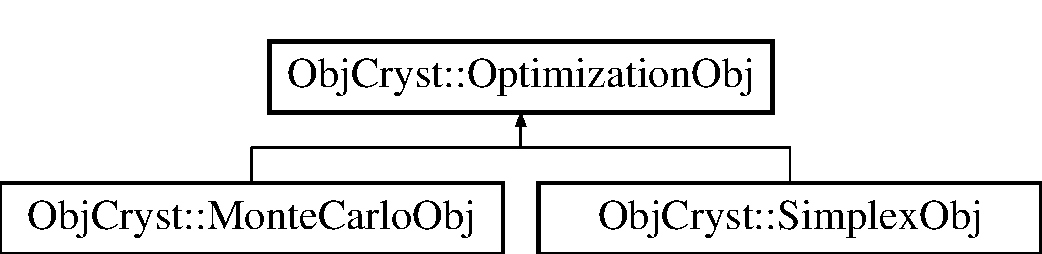
\includegraphics[height=2.000000cm]{a00061}
\end{center}
\end{figure}
\subsubsection*{Classes}
\begin{DoxyCompactItemize}
\item 
struct {\bf Log\+Likelihood\+Stats}
\begin{DoxyCompactList}\small\item\em Statistics about each object contributing to the overall Log(likelihood) \end{DoxyCompactList}\end{DoxyCompactItemize}
\subsubsection*{Public Member Functions}
\begin{DoxyCompactItemize}
\item 
{\bf Optimization\+Obj} (const string name=\char`\"{}\char`\"{})\label{a00061_a939444ac47768e16d205bebbc247cc12}

\begin{DoxyCompactList}\small\item\em Constructor. \end{DoxyCompactList}\item 
virtual {\bf $\sim$\+Optimization\+Obj} ()\label{a00061_a6fdf1e7158254a3c0a21b33e6ed5ffb5}

\begin{DoxyCompactList}\small\item\em Destructor. \end{DoxyCompactList}\item 
virtual void {\bf Randomize\+Starting\+Config} ()
\begin{DoxyCompactList}\small\item\em Randomize starting configuration. \end{DoxyCompactList}\item 
virtual void {\bf Optimize} (long \&nb\+Steps, const bool silent=false, const R\+E\+A\+L finalcost=0, const R\+E\+A\+L max\+Time=-\/1)=0
\begin{DoxyCompactList}\small\item\em Launch optimization (a single run) for N steps. \end{DoxyCompactList}\item 
virtual void {\bf Multi\+Run\+Optimize} (long \&nb\+Cycle, long \&nb\+Steps, const bool silent=false, const R\+E\+A\+L finalcost=0, const R\+E\+A\+L max\+Time=-\/1)=0
\begin{DoxyCompactList}\small\item\em Launch optimization for multiple runs of N steps. \end{DoxyCompactList}\item 
void {\bf Fix\+All\+Par} ()\label{a00061_af8b3cef84c6bcca37cdc4bfde9ecde45}

\begin{DoxyCompactList}\small\item\em Fix all parameters. \end{DoxyCompactList}\item 
void {\bf Set\+Par\+Is\+Fixed} (const string \&par\+Name, const bool fix)\label{a00061_aca3e1d2c6ace92f1a3a67da2455eac39}

\begin{DoxyCompactList}\small\item\em Fix one parameter. \end{DoxyCompactList}\item 
void {\bf Set\+Par\+Is\+Fixed} (const {\bf Ref\+Par\+Type} $\ast$type, const bool fix)\label{a00061_a12a66416a701cbf0db17de3bfafdec99}

\begin{DoxyCompactList}\small\item\em Fix one family of parameters. \end{DoxyCompactList}\item 
void {\bf Un\+Fix\+All\+Par} ()\label{a00061_adb016adacaa7a2a15e40cfb746705bdd}

\begin{DoxyCompactList}\small\item\em Un\+Fix All parameters. \end{DoxyCompactList}\item 
void {\bf Set\+Par\+Is\+Used} (const string \&par\+Name, const bool use)\label{a00061_ab2f87becfb73eb00d8f7c3ff25435c0d}

\begin{DoxyCompactList}\small\item\em Set a parameter to be used. \end{DoxyCompactList}\item 
void {\bf Set\+Par\+Is\+Used} (const {\bf Ref\+Par\+Type} $\ast$type, const bool use)\label{a00061_a73c29f094ad0a4923a2873388fc1eb93}

\begin{DoxyCompactList}\small\item\em Set a family of parameters to be used. \end{DoxyCompactList}\item 
void {\bf Set\+Limits\+Relative} (const string \&par\+Name, const R\+E\+A\+L min, const R\+E\+A\+L max)\label{a00061_a78113a7741eeda2263a27adcc24497c0}

\begin{DoxyCompactList}\small\item\em Change the relative limits for a parameter from its name. \end{DoxyCompactList}\item 
void {\bf Set\+Limits\+Relative} (const {\bf Ref\+Par\+Type} $\ast$type, const R\+E\+A\+L min, const R\+E\+A\+L max)\label{a00061_a0437fb441bebe91879de98efcb82865e}

\begin{DoxyCompactList}\small\item\em Change the relative limits for a family of parameter. \end{DoxyCompactList}\item 
void {\bf Set\+Limits\+Absolute} (const string \&par\+Name, const R\+E\+A\+L min, const R\+E\+A\+L max)\label{a00061_ad0bc0b36d1525526c55dc6642109d0b4}

\begin{DoxyCompactList}\small\item\em Change the absolute limits for a parameter from its name. \end{DoxyCompactList}\item 
void {\bf Set\+Limits\+Absolute} (const {\bf Ref\+Par\+Type} $\ast$type, const R\+E\+A\+L min, const R\+E\+A\+L max)\label{a00061_ade59b2e1d698ff7ba93ac5aa88187c58}

\begin{DoxyCompactList}\small\item\em Change the absolute limits for a family of parameter. \end{DoxyCompactList}\item 
virtual R\+E\+A\+L {\bf Get\+Log\+Likelihood} () const 
\begin{DoxyCompactList}\small\item\em The optimized (minimized, actually) function. \end{DoxyCompactList}\item 
void {\bf Stop\+After\+Cycle} ()\label{a00061_a288306acc3189c4fcaca398d11b32e4e}

\begin{DoxyCompactList}\small\item\em Stop after the current cycle. U\+Sed for interactive refinement. \end{DoxyCompactList}\item 
virtual void {\bf Display\+Report} ()\label{a00061_af09e8a9cd1b7f7f29bf57d027e08fc54}

\begin{DoxyCompactList}\small\item\em Show report to the user during refinement. Used for G\+U\+I update. \end{DoxyCompactList}\item 
void {\bf Add\+Refinable\+Obj} ({\bf Refinable\+Obj} \&)\label{a00061_a05e7019188763202126f9f83a31e1673}

\begin{DoxyCompactList}\small\item\em Add a refined object. All sub-\/objects are also added. \end{DoxyCompactList}\item 
{\bf Refinable\+Obj} \& {\bf Get\+Full\+Refinable\+Obj} (const bool rebuild=true)
\begin{DoxyCompactList}\small\item\em Get the \doxyref{Refinable\+Obj}{p.}{a00077} with all the parameters from all refined objects. \end{DoxyCompactList}\item 
virtual void {\bf X\+M\+L\+Output} (ostream \&os, int indent=0) const =0
\begin{DoxyCompactList}\small\item\em Output a description of the object in X\+M\+L format to a stream. \end{DoxyCompactList}\item 
virtual void {\bf X\+M\+L\+Input} (istream \&is, const {\bf X\+M\+L\+Cryst\+Tag} \&tag)=0
\begin{DoxyCompactList}\small\item\em Input in X\+M\+L format from a stream, restoring the set of refined objects and the associated cost functions. \end{DoxyCompactList}\item 
const string \& {\bf Get\+Name} () const \label{a00061_af595745274e554956834f885d7a1dc71}

\begin{DoxyCompactList}\small\item\em Get the name for this object. \end{DoxyCompactList}\item 
void {\bf Set\+Name} (const string \&)\label{a00061_a076dc80d878fc4ab5e5491f54642382e}

\begin{DoxyCompactList}\small\item\em Set the name for this object. \end{DoxyCompactList}\item 
virtual const string {\bf Get\+Class\+Name} () const \label{a00061_a2f00b2c3eb874d966bbb778a0d81abb1}

\begin{DoxyCompactList}\small\item\em Get the name for this class type. \end{DoxyCompactList}\item 
virtual void {\bf Print} () const \label{a00061_a55e92db45821ed13288d6852055c0003}

\begin{DoxyCompactList}\small\item\em Print some information about this object. \end{DoxyCompactList}\item 
void {\bf Restore\+Best\+Configuration} ()\label{a00061_a25a4ea1cf717a7d62ecf2cdbee87fa7a}

\begin{DoxyCompactList}\small\item\em Restore the Best configuration. \end{DoxyCompactList}\item 
bool {\bf Is\+Optimizing} () const \label{a00061_a02d12183cd9d167358717b87ada6ba1f}

\begin{DoxyCompactList}\small\item\em Are we busy optimizing ? \end{DoxyCompactList}\item 
void {\bf Tag\+New\+Best\+Config} ()\label{a00061_a99ca4e2216b0fd93ab335c35a99ca895}

\begin{DoxyCompactList}\small\item\em During a global optimization, tell all objects that the current config is the latest \char`\"{}best\char`\"{} config. \end{DoxyCompactList}\item 
R\+E\+A\+L {\bf Get\+Last\+Optim\+Elapsed\+Time} () const \label{a00061_af9bb37804ee3012cb05ffc217584db42}

\begin{DoxyCompactList}\small\item\em Get the elapsed time (in seconds) during the last optimization. \end{DoxyCompactList}\item 
{\bf Main\+Tracker} \& {\bf Get\+Main\+Tracker} ()\label{a00061_af8328b810bc37e45881e19948da7d2d7}

\begin{DoxyCompactList}\small\item\em Get the \doxyref{Main\+Tracker}{p.}{a00047}. \end{DoxyCompactList}\item 
const {\bf Main\+Tracker} \& {\bf Get\+Main\+Tracker} () const \label{a00061_a737490fc1ac0b30fc3bb3a5bb8061a8b}

\begin{DoxyCompactList}\small\item\em Get the \doxyref{Main\+Tracker}{p.}{a00047}. \end{DoxyCompactList}\item 
{\bf Ref\+Obj\+Opt} \& {\bfseries Get\+X\+M\+L\+Auto\+Save\+Option} ()\label{a00061_a82e4adbc7b5d3374f7c414a0e89c25fd}

\item 
const {\bf Ref\+Obj\+Opt} \& {\bfseries Get\+X\+M\+L\+Auto\+Save\+Option} () const \label{a00061_a0a37e6bcce21926e13a3f57882e971b0}

\item 
const R\+E\+A\+L \& {\bf Get\+Best\+Cost} () const \label{a00061_a56c9ec94e7632c8b3f36e3a837c02594}

\begin{DoxyCompactList}\small\item\em Access to current best cost. \end{DoxyCompactList}\item 
R\+E\+A\+L \& {\bf Get\+Best\+Cost} ()\label{a00061_a894882f10bd768e3e57ffdfa9f9df7fe}

\begin{DoxyCompactList}\small\item\em Access to current best cost. \end{DoxyCompactList}\item 
virtual void {\bf Begin\+Optimization} (const bool allow\+Approximations=false, const bool enable\+Restraints=false)\label{a00061_a13c12dbdc72825f892c3d48dd2b6cfe3}

\begin{DoxyCompactList}\small\item\em Begin optimization for all objects. \end{DoxyCompactList}\item 
virtual void {\bf End\+Optimization} ()\label{a00061_a37c2335ad867152121253996daaebc6e}

\begin{DoxyCompactList}\small\item\em End optimization for all objects. \end{DoxyCompactList}\end{DoxyCompactItemize}
\subsubsection*{Protected Member Functions}
\begin{DoxyCompactItemize}
\item 
void {\bf Prepare\+Ref\+Par\+List} ()
\item 
virtual void {\bf Init\+Options} ()\label{a00061_a0d7f6ae8f6ef49b59f0bc5b4794931e9}

\begin{DoxyCompactList}\small\item\em Initialization of options. \end{DoxyCompactList}\item 
virtual void {\bf Update\+Display} ()
\begin{DoxyCompactList}\small\item\em Update Display (if any display is available), when a new 'relevant' configuration is reached. \end{DoxyCompactList}\item 
void {\bf Build\+Recursive\+Ref\+Obj\+List} ()
\begin{DoxyCompactList}\small\item\em (Re)build \doxyref{Optimization\+Obj\+::m\+Recursive\+Refined\+Obj\+List}{p.}{a00061_a0e6a9e9d4d12ed73c582da36190f110f}, if an object has been added or modified. \end{DoxyCompactList}\end{DoxyCompactItemize}
\subsubsection*{Protected Attributes}
\begin{DoxyCompactItemize}
\item 
{\bf Refinable\+Obj} {\bf m\+Ref\+Par\+List}
\begin{DoxyCompactList}\small\item\em The refinable par list used during refinement. \end{DoxyCompactList}\item 
string {\bf m\+Name}\label{a00061_a9fa42c95df26834a9f369af61eb10ea6}

\begin{DoxyCompactList}\small\item\em Name of the Global\+Optimization object. \end{DoxyCompactList}\item 
string {\bf m\+Save\+File\+Name}\label{a00061_a2694dd9fc6ab088e3d79e0c9e0358311}

\begin{DoxyCompactList}\small\item\em File name where refinement info is saved (N\+O\+T U\+S\+E\+D so far...) \end{DoxyCompactList}\item 
long {\bf m\+Nb\+Trial}\label{a00061_af47650ca783520dd0100077b08271c79}

\begin{DoxyCompactList}\small\item\em Number of trials so far. \end{DoxyCompactList}\item 
R\+E\+A\+L {\bf m\+Best\+Cost}\label{a00061_a495926a48dd408a3b92de8a6b33f815a}

\begin{DoxyCompactList}\small\item\em Best value of the cost function so far. \end{DoxyCompactList}\item 
long {\bf m\+Best\+Par\+Saved\+Set\+Index}\label{a00061_aa9c2d238f7b60c7ea3bd715bf145b5d3}

\begin{DoxyCompactList}\small\item\em Index of the 'best' saved parameter set. \end{DoxyCompactList}\item 
unsigned long {\bf m\+Context}\label{a00061_a7139f75c5b214ea00f99c2e4c25b2b34}

\begin{DoxyCompactList}\small\item\em The current 'context', in the case the optimization is run in different parallel contexts. \end{DoxyCompactList}\item 
map$<$ unsigned long, map$<$ const \\*
{\bf Refinable\+Obj} \\*
$\ast$, {\bf Log\+Likelihood\+Stats} $>$ $>$ {\bf mv\+Context\+Obj\+Stats}\label{a00061_a1b33baa71f4e0b182bae66766608425f}

\begin{DoxyCompactList}\small\item\em Statistics for each context (mutable for dynamic update during optimization) \end{DoxyCompactList}\item 
map$<$ const {\bf Refinable\+Obj} \\*
$\ast$, Dynamic\+Obj\+Weight $>$ {\bf mv\+Obj\+Weight}\label{a00061_a4b1120b0a6fc24c82c273152722f672c}

\begin{DoxyCompactList}\small\item\em Weights for each objects in each context (mutable for dynamic update during optimization) \end{DoxyCompactList}\item 
std\+::vector$<$ pair$<$ long, R\+E\+A\+L $>$ $>$ {\bf mv\+Saved\+Param\+Set}
\begin{DoxyCompactList}\small\item\em List of saved parameter sets. \end{DoxyCompactList}\item 
bool {\bf m\+Is\+Optimizing}\label{a00061_a712048cd592825ce31ced1120733345b}

\begin{DoxyCompactList}\small\item\em True if a refinement is being done. For multi-\/threaded environment. \end{DoxyCompactList}\item 
bool {\bf m\+Stop\+After\+Cycle}\label{a00061_abec493a46c9e57c7e71e886bcae601fb}

\begin{DoxyCompactList}\small\item\em If true, then stop at the end of the cycle. Used in multi-\/threaded environment. \end{DoxyCompactList}\item 
{\bf Obj\+Registry}$<$ {\bf Refinable\+Obj} $>$ {\bf m\+Refined\+Obj\+List}\label{a00061_a73f491b5c8a0ae5f087e496916f76016}

\begin{DoxyCompactList}\small\item\em The refined objects. \end{DoxyCompactList}\item 
{\bf Obj\+Registry}$<$ {\bf Refinable\+Obj} $>$ {\bf m\+Recursive\+Refined\+Obj\+List}
\begin{DoxyCompactList}\small\item\em The refined objects, recursively including all sub-\/objects. \end{DoxyCompactList}\item 
{\bf Ref\+Obj\+Opt} {\bf m\+X\+M\+L\+Auto\+Save}\label{a00061_a94038e1c477b1efa6417c13106d6bc89}

\begin{DoxyCompactList}\small\item\em Periodic save of complete environment as an xml file. \end{DoxyCompactList}\item 
R\+E\+A\+L {\bf m\+Last\+Optim\+Time}\label{a00061_abf309e1b2248a7e1d3744d4b20d15bfd}

\begin{DoxyCompactList}\small\item\em The time elapsed after the last optimization, in seconds. \end{DoxyCompactList}\item 
{\bf Main\+Tracker} {\bf m\+Main\+Tracker}
\begin{DoxyCompactList}\small\item\em \doxyref{Main\+Tracker}{p.}{a00047} object to track the evolution of cost functions, likelihood, and individual parameters. \end{DoxyCompactList}\end{DoxyCompactItemize}


\subsubsection{Detailed Description}
Base object for Optimization methods. 

This is an abstract base class, derived for Monte-\/\+Cralo type algorithms (Simulated Annealing \& Parallel Tempering), and hopefully soon for Genetic Algorithms.

\begin{DoxyRemark}{Remarks}
Instead of keeping a copy of the list of parameters here, maybe it would be better to delegate all parameter handling to the refined objects (they would also have to keep in memory the saved parameter sets, so that could be difficult to administrate...). 
\end{DoxyRemark}


\subsubsection{Member Function Documentation}
\index{Obj\+Cryst\+::\+Optimization\+Obj@{Obj\+Cryst\+::\+Optimization\+Obj}!Build\+Recursive\+Ref\+Obj\+List@{Build\+Recursive\+Ref\+Obj\+List}}
\index{Build\+Recursive\+Ref\+Obj\+List@{Build\+Recursive\+Ref\+Obj\+List}!Obj\+Cryst\+::\+Optimization\+Obj@{Obj\+Cryst\+::\+Optimization\+Obj}}
\paragraph[{Build\+Recursive\+Ref\+Obj\+List}]{\setlength{\rightskip}{0pt plus 5cm}void Obj\+Cryst\+::\+Optimization\+Obj\+::\+Build\+Recursive\+Ref\+Obj\+List (
\begin{DoxyParamCaption}
{}
\end{DoxyParamCaption}
)\hspace{0.3cm}{\ttfamily [protected]}}\label{a00061_a7c819c5f8fc52caafd97ea9d468da2be}


(Re)build \doxyref{Optimization\+Obj\+::m\+Recursive\+Refined\+Obj\+List}{p.}{a00061_a0e6a9e9d4d12ed73c582da36190f110f}, if an object has been added or modified. 

If no object has been added and no sub-\/object has been added/removed, then nothing is done. \index{Obj\+Cryst\+::\+Optimization\+Obj@{Obj\+Cryst\+::\+Optimization\+Obj}!Get\+Full\+Refinable\+Obj@{Get\+Full\+Refinable\+Obj}}
\index{Get\+Full\+Refinable\+Obj@{Get\+Full\+Refinable\+Obj}!Obj\+Cryst\+::\+Optimization\+Obj@{Obj\+Cryst\+::\+Optimization\+Obj}}
\paragraph[{Get\+Full\+Refinable\+Obj}]{\setlength{\rightskip}{0pt plus 5cm}{\bf Refinable\+Obj}\& Obj\+Cryst\+::\+Optimization\+Obj\+::\+Get\+Full\+Refinable\+Obj (
\begin{DoxyParamCaption}
\item[{const bool}]{rebuild = {\ttfamily true}}
\end{DoxyParamCaption}
)}\label{a00061_afef162d94382a93fe037fac1b5d3ef03}


Get the \doxyref{Refinable\+Obj}{p.}{a00077} with all the parameters from all refined objects. 

If rebuild=true, prepare again the list of objects/parameters. \index{Obj\+Cryst\+::\+Optimization\+Obj@{Obj\+Cryst\+::\+Optimization\+Obj}!Get\+Log\+Likelihood@{Get\+Log\+Likelihood}}
\index{Get\+Log\+Likelihood@{Get\+Log\+Likelihood}!Obj\+Cryst\+::\+Optimization\+Obj@{Obj\+Cryst\+::\+Optimization\+Obj}}
\paragraph[{Get\+Log\+Likelihood}]{\setlength{\rightskip}{0pt plus 5cm}virtual R\+E\+A\+L Obj\+Cryst\+::\+Optimization\+Obj\+::\+Get\+Log\+Likelihood (
\begin{DoxyParamCaption}
{}
\end{DoxyParamCaption}
) const\hspace{0.3cm}{\ttfamily [virtual]}}\label{a00061_a0f317f235e6e5cb1867cc7c5870f510f}


The optimized (minimized, actually) function. 

This function is the weighted sum of the chosen Cost Functions for the refined objects. \index{Obj\+Cryst\+::\+Optimization\+Obj@{Obj\+Cryst\+::\+Optimization\+Obj}!Multi\+Run\+Optimize@{Multi\+Run\+Optimize}}
\index{Multi\+Run\+Optimize@{Multi\+Run\+Optimize}!Obj\+Cryst\+::\+Optimization\+Obj@{Obj\+Cryst\+::\+Optimization\+Obj}}
\paragraph[{Multi\+Run\+Optimize}]{\setlength{\rightskip}{0pt plus 5cm}virtual void Obj\+Cryst\+::\+Optimization\+Obj\+::\+Multi\+Run\+Optimize (
\begin{DoxyParamCaption}
\item[{long \&}]{nb\+Cycle, }
\item[{long \&}]{nb\+Steps, }
\item[{const bool}]{silent = {\ttfamily false}, }
\item[{const R\+E\+A\+L}]{finalcost = {\ttfamily 0}, }
\item[{const R\+E\+A\+L}]{max\+Time = {\ttfamily -\/1}}
\end{DoxyParamCaption}
)\hspace{0.3cm}{\ttfamily [pure virtual]}}\label{a00061_aa53575dbda2ec3f561bed934beb4ca6f}


Launch optimization for multiple runs of N steps. 


\begin{DoxyParams}{Parameters}
{\em nb\+Cycle} & the number of runs (cycles) to perform. The structure is randomized at the beginning of each cycle. If nb\+Cycle==-\/1, this will run indefinitely. The nb\+Cycle parameter is decreased after each run. \\
\hline
{\em nb\+Steps} & the number of steps to go. This number is modified (decreases!) as the refinement goes on. \\
\hline
{\em silent} & \+: if true, absolutely no message should be printed (except debugging) \\
\hline
{\em finalcost} & the optimization will stop if overall cost fallse below this value \\
\hline
{\em max\+Time} & the optimization will stop after the given number of seconds has been spent optimizing (ignored if $<$0). \\
\hline
\end{DoxyParams}


Implemented in {\bf Obj\+Cryst\+::\+Monte\+Carlo\+Obj} \doxyref{}{p.}{a00056_ae1689aa2dd5867499768328df935334d}, and {\bf Obj\+Cryst\+::\+Simplex\+Obj} \doxyref{}{p.}{a00099_a1c7ae823f9e31169b453f36d15c049b8}.

\index{Obj\+Cryst\+::\+Optimization\+Obj@{Obj\+Cryst\+::\+Optimization\+Obj}!Optimize@{Optimize}}
\index{Optimize@{Optimize}!Obj\+Cryst\+::\+Optimization\+Obj@{Obj\+Cryst\+::\+Optimization\+Obj}}
\paragraph[{Optimize}]{\setlength{\rightskip}{0pt plus 5cm}virtual void Obj\+Cryst\+::\+Optimization\+Obj\+::\+Optimize (
\begin{DoxyParamCaption}
\item[{long \&}]{nb\+Steps, }
\item[{const bool}]{silent = {\ttfamily false}, }
\item[{const R\+E\+A\+L}]{finalcost = {\ttfamily 0}, }
\item[{const R\+E\+A\+L}]{max\+Time = {\ttfamily -\/1}}
\end{DoxyParamCaption}
)\hspace{0.3cm}{\ttfamily [pure virtual]}}\label{a00061_a08c77dc6ec80f63bf067ef2968a0b6dc}


Launch optimization (a single run) for N steps. 


\begin{DoxyParams}{Parameters}
{\em nb\+Steps} & the number of steps to go. This number is modified (decreases!) as the refinement goes on. \\
\hline
{\em silent} & \+: if true, absolutely no message should be printed (except debugging) \\
\hline
{\em finalcost} & the optimization will stop if overall cost fallse below this value \\
\hline
{\em max\+Time} & the optimization will stop after the given number of seconds has been spent optimizing (ignored if $<$0). \\
\hline
\end{DoxyParams}


Implemented in {\bf Obj\+Cryst\+::\+Monte\+Carlo\+Obj} \doxyref{}{p.}{a00056_aef060de8a302fb8c4e607e00667d7b49}, and {\bf Obj\+Cryst\+::\+Simplex\+Obj} \doxyref{}{p.}{a00099_aa8bf4b209e2ce6229722b18ec9911010}.

\index{Obj\+Cryst\+::\+Optimization\+Obj@{Obj\+Cryst\+::\+Optimization\+Obj}!Prepare\+Ref\+Par\+List@{Prepare\+Ref\+Par\+List}}
\index{Prepare\+Ref\+Par\+List@{Prepare\+Ref\+Par\+List}!Obj\+Cryst\+::\+Optimization\+Obj@{Obj\+Cryst\+::\+Optimization\+Obj}}
\paragraph[{Prepare\+Ref\+Par\+List}]{\setlength{\rightskip}{0pt plus 5cm}void Obj\+Cryst\+::\+Optimization\+Obj\+::\+Prepare\+Ref\+Par\+List (
\begin{DoxyParamCaption}
{}
\end{DoxyParamCaption}
)\hspace{0.3cm}{\ttfamily [protected]}}\label{a00061_a2f11f520bc1bd0b70f8aea98d3f8224c}
Prepare m\+Ref\+Par\+List for the refinement \index{Obj\+Cryst\+::\+Optimization\+Obj@{Obj\+Cryst\+::\+Optimization\+Obj}!Randomize\+Starting\+Config@{Randomize\+Starting\+Config}}
\index{Randomize\+Starting\+Config@{Randomize\+Starting\+Config}!Obj\+Cryst\+::\+Optimization\+Obj@{Obj\+Cryst\+::\+Optimization\+Obj}}
\paragraph[{Randomize\+Starting\+Config}]{\setlength{\rightskip}{0pt plus 5cm}virtual void Obj\+Cryst\+::\+Optimization\+Obj\+::\+Randomize\+Starting\+Config (
\begin{DoxyParamCaption}
{}
\end{DoxyParamCaption}
)\hspace{0.3cm}{\ttfamily [virtual]}}\label{a00061_a04ac9f4d67eb8823b78b00f222a5a29c}


Randomize starting configuration. 

Only affects limited and periodic parameters. \index{Obj\+Cryst\+::\+Optimization\+Obj@{Obj\+Cryst\+::\+Optimization\+Obj}!Update\+Display@{Update\+Display}}
\index{Update\+Display@{Update\+Display}!Obj\+Cryst\+::\+Optimization\+Obj@{Obj\+Cryst\+::\+Optimization\+Obj}}
\paragraph[{Update\+Display}]{\setlength{\rightskip}{0pt plus 5cm}virtual void Obj\+Cryst\+::\+Optimization\+Obj\+::\+Update\+Display (
\begin{DoxyParamCaption}
{}
\end{DoxyParamCaption}
)\hspace{0.3cm}{\ttfamily [protected]}, {\ttfamily [virtual]}}\label{a00061_a3658f0e6232756d68b8b17256f27a9bd}


Update Display (if any display is available), when a new 'relevant' configuration is reached. 

This calls all \doxyref{Refinable\+Obj\+::\+Update\+Display()}{p.}{a00077_ab74e2cead734fe1e652c5add46c5e116} \index{Obj\+Cryst\+::\+Optimization\+Obj@{Obj\+Cryst\+::\+Optimization\+Obj}!X\+M\+L\+Input@{X\+M\+L\+Input}}
\index{X\+M\+L\+Input@{X\+M\+L\+Input}!Obj\+Cryst\+::\+Optimization\+Obj@{Obj\+Cryst\+::\+Optimization\+Obj}}
\paragraph[{X\+M\+L\+Input}]{\setlength{\rightskip}{0pt plus 5cm}virtual void Obj\+Cryst\+::\+Optimization\+Obj\+::\+X\+M\+L\+Input (
\begin{DoxyParamCaption}
\item[{istream \&}]{is, }
\item[{const {\bf X\+M\+L\+Cryst\+Tag} \&}]{tag}
\end{DoxyParamCaption}
)\hspace{0.3cm}{\ttfamily [pure virtual]}}\label{a00061_aa07aee60f56780e2c56fb20f4a5f48a8}


Input in X\+M\+L format from a stream, restoring the set of refined objects and the associated cost functions. 

Note that the corresponding objects must have been loaded in memory before, else shit happens. 

Implemented in {\bf Obj\+Cryst\+::\+Monte\+Carlo\+Obj} \doxyref{}{p.}{a00056_a2f9428857b1d26bbdac08d59debb9f52}, and {\bf Obj\+Cryst\+::\+Simplex\+Obj} \doxyref{}{p.}{a00099_ae6ed0602ffdd2db1a10be80820a0a285}.

\index{Obj\+Cryst\+::\+Optimization\+Obj@{Obj\+Cryst\+::\+Optimization\+Obj}!X\+M\+L\+Output@{X\+M\+L\+Output}}
\index{X\+M\+L\+Output@{X\+M\+L\+Output}!Obj\+Cryst\+::\+Optimization\+Obj@{Obj\+Cryst\+::\+Optimization\+Obj}}
\paragraph[{X\+M\+L\+Output}]{\setlength{\rightskip}{0pt plus 5cm}virtual void Obj\+Cryst\+::\+Optimization\+Obj\+::\+X\+M\+L\+Output (
\begin{DoxyParamCaption}
\item[{ostream \&}]{os, }
\item[{int}]{indent = {\ttfamily 0}}
\end{DoxyParamCaption}
) const\hspace{0.3cm}{\ttfamily [pure virtual]}}\label{a00061_a6b7726159bb0d5dad1c7eebaee78f53a}


Output a description of the object in X\+M\+L format to a stream. 

This saves the list of refined object and the cost functions, as well as options for the refinement. The refined objects are {\bfseries not} saved, so this must be done somewhere else (they must be reloaded before this object). 

Implemented in {\bf Obj\+Cryst\+::\+Monte\+Carlo\+Obj} \doxyref{}{p.}{a00056_a619eb171e5fe384be4d37f999dde8e0f}, and {\bf Obj\+Cryst\+::\+Simplex\+Obj} \doxyref{}{p.}{a00099_a7111042ca3a7201039a25fe548cb524c}.



\subsubsection{Member Data Documentation}
\index{Obj\+Cryst\+::\+Optimization\+Obj@{Obj\+Cryst\+::\+Optimization\+Obj}!m\+Main\+Tracker@{m\+Main\+Tracker}}
\index{m\+Main\+Tracker@{m\+Main\+Tracker}!Obj\+Cryst\+::\+Optimization\+Obj@{Obj\+Cryst\+::\+Optimization\+Obj}}
\paragraph[{m\+Main\+Tracker}]{\setlength{\rightskip}{0pt plus 5cm}{\bf Main\+Tracker} Obj\+Cryst\+::\+Optimization\+Obj\+::m\+Main\+Tracker\hspace{0.3cm}{\ttfamily [protected]}}\label{a00061_abe2f9a9812abe0f4a6c414457b5b2967}


\doxyref{Main\+Tracker}{p.}{a00047} object to track the evolution of cost functions, likelihood, and individual parameters. 

\index{Obj\+Cryst\+::\+Optimization\+Obj@{Obj\+Cryst\+::\+Optimization\+Obj}!m\+Recursive\+Refined\+Obj\+List@{m\+Recursive\+Refined\+Obj\+List}}
\index{m\+Recursive\+Refined\+Obj\+List@{m\+Recursive\+Refined\+Obj\+List}!Obj\+Cryst\+::\+Optimization\+Obj@{Obj\+Cryst\+::\+Optimization\+Obj}}
\paragraph[{m\+Recursive\+Refined\+Obj\+List}]{\setlength{\rightskip}{0pt plus 5cm}{\bf Obj\+Registry}$<${\bf Refinable\+Obj}$>$ Obj\+Cryst\+::\+Optimization\+Obj\+::m\+Recursive\+Refined\+Obj\+List\hspace{0.3cm}{\ttfamily [mutable]}, {\ttfamily [protected]}}\label{a00061_a0e6a9e9d4d12ed73c582da36190f110f}


The refined objects, recursively including all sub-\/objects. 

This is mutable, since it is a function of m\+Refined\+Obj\+List only. \index{Obj\+Cryst\+::\+Optimization\+Obj@{Obj\+Cryst\+::\+Optimization\+Obj}!m\+Ref\+Par\+List@{m\+Ref\+Par\+List}}
\index{m\+Ref\+Par\+List@{m\+Ref\+Par\+List}!Obj\+Cryst\+::\+Optimization\+Obj@{Obj\+Cryst\+::\+Optimization\+Obj}}
\paragraph[{m\+Ref\+Par\+List}]{\setlength{\rightskip}{0pt plus 5cm}{\bf Refinable\+Obj} Obj\+Cryst\+::\+Optimization\+Obj\+::m\+Ref\+Par\+List\hspace{0.3cm}{\ttfamily [mutable]}, {\ttfamily [protected]}}\label{a00061_a9cf13c38f24b4b2ddd6cb239286053af}


The refinable par list used during refinement. 

Only a condensed version of all objects. This is useful to keep an history of modifications, and to restore previous values. \begin{DoxyRemark}{Remarks}
maybe this should be completely delegated to the refined objetcs. 
\end{DoxyRemark}
\index{Obj\+Cryst\+::\+Optimization\+Obj@{Obj\+Cryst\+::\+Optimization\+Obj}!mv\+Saved\+Param\+Set@{mv\+Saved\+Param\+Set}}
\index{mv\+Saved\+Param\+Set@{mv\+Saved\+Param\+Set}!Obj\+Cryst\+::\+Optimization\+Obj@{Obj\+Cryst\+::\+Optimization\+Obj}}
\paragraph[{mv\+Saved\+Param\+Set}]{\setlength{\rightskip}{0pt plus 5cm}std\+::vector$<$pair$<$long,R\+E\+A\+L$>$ $>$ Obj\+Cryst\+::\+Optimization\+Obj\+::mv\+Saved\+Param\+Set\hspace{0.3cm}{\ttfamily [protected]}}\label{a00061_a9063bb2fa6a6f0938295be2ffe2bfe84}


List of saved parameter sets. 

This is used to save possible solutions during the optimization, so that the user can check them afterwards.

The first member of each pair is the {\itshape index} of the parameter set, and the second is the overall cost for that set. 

The documentation for this class was generated from the following file\+:\begin{DoxyCompactItemize}
\item 
Global\+Optim\+Obj.\+h\end{DoxyCompactItemize}

\subsection{Obj\-Cryst\-:\-:P\-D\-F Class Reference}
\label{a00062}\index{Obj\-Cryst\-::\-P\-D\-F@{Obj\-Cryst\-::\-P\-D\-F}}


Main class for Pair distribution function calculations and comparison to observed one.  


Inheritance diagram for Obj\-Cryst\-:\-:P\-D\-F\-:\begin{figure}[H]
\begin{center}
\leavevmode
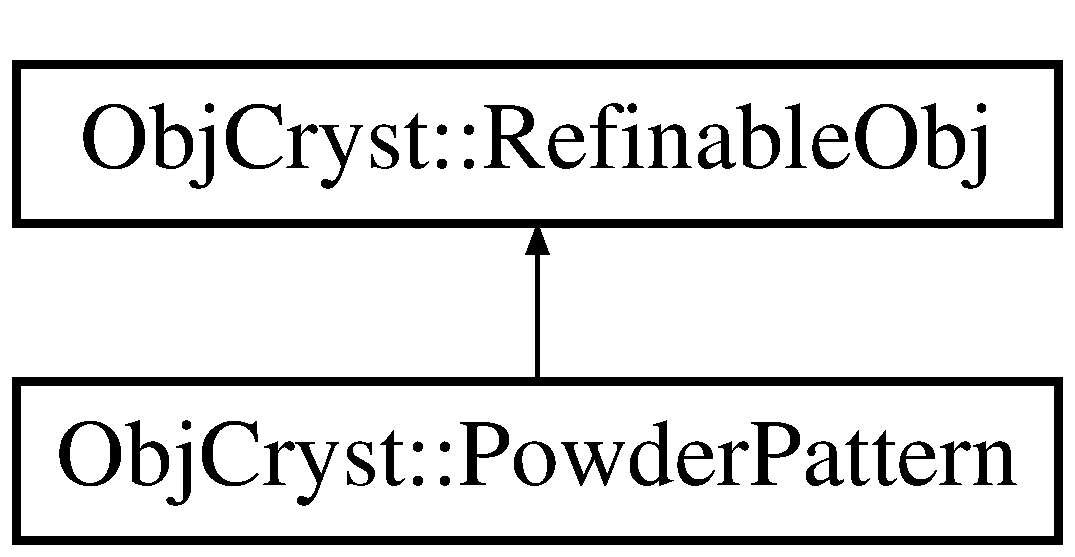
\includegraphics[height=2.000000cm]{a00062}
\end{center}
\end{figure}
\subsubsection*{Public Member Functions}
\begin{DoxyCompactItemize}
\item 
{\bf P\-D\-F} (const {\bf P\-D\-F} \&old)\label{a00062_af5633baa0e58aa65b1a7cf80cfb79712}

\begin{DoxyCompactList}\small\item\em Copy constructor. \end{DoxyCompactList}\item 
{\bf $\sim$\-P\-D\-F} ()\label{a00062_adf8dacf02c0b3a6c8f49d86daa25b527}

\begin{DoxyCompactList}\small\item\em \doxyref{Crystal}{p.}{a00026} destructor. \end{DoxyCompactList}\item 
virtual const string \& {\bf Get\-Class\-Name} () const 
\begin{DoxyCompactList}\small\item\em Name for this class (\char`\"{}\-Refinable\-Obj\char`\"{}, \char`\"{}\-Crystal\char`\"{},...). \end{DoxyCompactList}\item 
void {\bf Set\-P\-D\-F\-Obs} (const Cryst\-Vector\-\_\-\-R\-E\-A\-L \&r, const Cryst\-Vector\-\_\-\-R\-E\-A\-L \&obs)\label{a00062_a7ff4d297dca6974e099ad5b45d6b9ffa}

\begin{DoxyCompactList}\small\item\em Experimental data. \end{DoxyCompactList}\item 
{\bf Radiation\-Type} {\bf Get\-Radiation\-Type} () const \label{a00062_a940341ae04811d1b0bdf87c72ba594b5}

\begin{DoxyCompactList}\small\item\em Get\-Radiation\-Type. \end{DoxyCompactList}\item 
void {\bf Set\-Radiation\-Type} ({\bf Radiation\-Type} type)\label{a00062_a51d1cebecb13d8e60038fca30547c84e}

\begin{DoxyCompactList}\small\item\em Set\-Radiation\-Type. \end{DoxyCompactList}\item 
R\-E\-A\-L {\bf Get\-R\-Max} () const \label{a00062_a00503dc494bffe09c7ae85d29e2a339e}

\begin{DoxyCompactList}\small\item\em Cutoff r value. \end{DoxyCompactList}\item 
const Cryst\-Vector\-\_\-\-R\-E\-A\-L \& {\bf Get\-P\-D\-F\-Calc} () const \label{a00062_a741872ecb602f9721b77c7b255f56876}

\begin{DoxyCompactList}\small\item\em Get the calculated \doxyref{P\-D\-F}{p.}{a00062}. \end{DoxyCompactList}\item 
const Cryst\-Vector\-\_\-\-R\-E\-A\-L \& {\bf Get\-P\-D\-F\-Obs} () const \label{a00062_a09dcfddbc9ec6bf33726675dad856fe4}

\begin{DoxyCompactList}\small\item\em Get the observed \doxyref{P\-D\-F}{p.}{a00062}. \end{DoxyCompactList}\item 
const Cryst\-Vector\-\_\-\-R\-E\-A\-L \& {\bf Get\-P\-D\-F\-R} () const \label{a00062_a79778c610b24aee1caedaa011a8ec0fb}

\begin{DoxyCompactList}\small\item\em Get the r coordinates (in Angstroem) for the \doxyref{P\-D\-F}{p.}{a00062}. \end{DoxyCompactList}\item 
void {\bf Add\-P\-D\-F\-Phase} ({\bf P\-D\-F\-Phase} \&phase)\label{a00062_a4a39ea9bce2350b5786575fc4fc7a9ea}

\begin{DoxyCompactList}\small\item\em Add \doxyref{P\-D\-F}{p.}{a00062} phase. \end{DoxyCompactList}\end{DoxyCompactItemize}
\subsubsection*{Private Attributes}
\begin{DoxyCompactItemize}
\item 
{\bf Radiation\-Type} {\bf m\-Radiation\-Type}\label{a00062_af3ab577cb12f62f38fbd3a6d88e242bf}

\begin{DoxyCompactList}\small\item\em \doxyref{Radiation}{p.}{a00075} type. \end{DoxyCompactList}\item 
Cryst\-Vector\-\_\-\-R\-E\-A\-L {\bf m\-P\-D\-F\-R}\label{a00062_a49cadbd04ae733321638566defc3a246}

\begin{DoxyCompactList}\small\item\em r coordinates (in Angstroem) of the \doxyref{P\-D\-F}{p.}{a00062} \end{DoxyCompactList}\item 
Cryst\-Vector\-\_\-\-R\-E\-A\-L {\bf m\-P\-D\-F\-Calc}\label{a00062_a6a907317c064f14614b5c55456de42b0}

\begin{DoxyCompactList}\small\item\em The \doxyref{P\-D\-F}{p.}{a00062} itself,calculated. \end{DoxyCompactList}\item 
Cryst\-Vector\-\_\-\-R\-E\-A\-L {\bf m\-P\-D\-F\-Obs}\label{a00062_a7cc4d168934d80fdea6f22c3f2789ff3}

\begin{DoxyCompactList}\small\item\em The \doxyref{P\-D\-F}{p.}{a00062} itself,observed. \end{DoxyCompactList}\item 
std\-::list$<$ std\-::pair$<$ {\bf P\-D\-F\-Phase} \\*
$\ast$, R\-E\-A\-L $>$ $>$ {\bf mv\-P\-D\-F\-Phase}\label{a00062_aa389a686162b7341ba62a2dffafb0d7b}

\begin{DoxyCompactList}\small\item\em Contributions to the \doxyref{P\-D\-F}{p.}{a00062}, with their scale factor. \end{DoxyCompactList}\end{DoxyCompactItemize}
\subsubsection*{Additional Inherited Members}


\subsubsection{Detailed Description}
Main class for Pair distribution function calculations and comparison to observed one. 



\subsubsection{Member Function Documentation}
\index{Obj\-Cryst\-::\-P\-D\-F@{Obj\-Cryst\-::\-P\-D\-F}!Get\-Class\-Name@{Get\-Class\-Name}}
\index{Get\-Class\-Name@{Get\-Class\-Name}!ObjCryst::PDF@{Obj\-Cryst\-::\-P\-D\-F}}
\paragraph[{Get\-Class\-Name}]{\setlength{\rightskip}{0pt plus 5cm}virtual const string\& Obj\-Cryst\-::\-P\-D\-F\-::\-Get\-Class\-Name (
\begin{DoxyParamCaption}
{}
\end{DoxyParamCaption}
) const\hspace{0.3cm}{\ttfamily [virtual]}}\label{a00062_a809ab3f4cc8bdd268bd815baedccdc20}


Name for this class (\char`\"{}\-Refinable\-Obj\char`\"{}, \char`\"{}\-Crystal\char`\"{},...). 

This is only useful to distinguish different classes when picking up objects from the \doxyref{Refinable\-Obj}{p.}{a00077} Global Registry 

Reimplemented from {\bf Obj\-Cryst\-::\-Refinable\-Obj} \doxyref{}{p.}{a00077_a62968d90a7a3080738b363934616c019}.



The documentation for this class was generated from the following file\-:\begin{DoxyCompactItemize}
\item 
P\-D\-F.\-h\end{DoxyCompactItemize}

\subsection{Obj\-Cryst\-:\-:P\-D\-F\-Crystal\-:\-:pdf\-Atom Struct Reference}
\label{a00063}\index{Obj\-Cryst\-::\-P\-D\-F\-Crystal\-::pdf\-Atom@{Obj\-Cryst\-::\-P\-D\-F\-Crystal\-::pdf\-Atom}}


Container of temp data for each atom.  


\subsubsection*{Public Member Functions}
\begin{DoxyCompactItemize}
\item 
{\bf pdf\-Atom} ()\label{a00063_a3909167af1d0f03dd62d1a7b07524aaa}

\begin{DoxyCompactList}\small\item\em default constructor \end{DoxyCompactList}\end{DoxyCompactItemize}
\subsubsection*{Public Attributes}
\begin{DoxyCompactItemize}
\item 
R\-E\-A\-L {\bf fx0}\label{a00063_a64a01ae0646a38e7ec6aacc32879293b}

\begin{DoxyCompactList}\small\item\em Fractionnal \& cartesian unique coordinates. \end{DoxyCompactList}\item 
R\-E\-A\-L {\bfseries fy0}\label{a00063_a842098b3e4c330de75d81360430bff2b}

\item 
R\-E\-A\-L {\bfseries fz0}\label{a00063_a869b4043afffd73fa4691075b9cf49fb}

\item 
R\-E\-A\-L {\bfseries x0}\label{a00063_a684db85285aafa127dcc2b3ab1ee705e}

\item 
R\-E\-A\-L {\bfseries y0}\label{a00063_a33fc5fb326d440de0c4e27a45eac3bee}

\item 
R\-E\-A\-L {\bfseries z0}\label{a00063_a62c30b98c58028facfcac46ca7773754}

\item 
const {\bf Scattering\-Power} $\ast$ {\bf p\-Scatt\-Pow}\label{a00063_ac9fb4e85c6a68222212b4e0fc35dc45d}

\begin{DoxyCompactList}\small\item\em The scattering power. \end{DoxyCompactList}\item 
R\-E\-A\-L {\bf occup\-Bi}\label{a00063_aba908a68756273eda5261980e574dfef}

\begin{DoxyCompactList}\small\item\em Scattering amplitudes, multiplied by occupancy. \end{DoxyCompactList}\item 
bool {\bf has\-Changed}\label{a00063_a273d054875caabd824b8d1f4ee12cc22}

\begin{DoxyCompactList}\small\item\em Has this atom changed since last time ? \end{DoxyCompactList}\item 
Cryst\-Vector\-\_\-\-R\-E\-A\-L {\bf x}\label{a00063_a807d379b04bd1c18c64b8636060577bf}

\begin{DoxyCompactList}\small\item\em List of all equivalent \& translated positions, in cartesian coordinates. \end{DoxyCompactList}\item 
Cryst\-Vector\-\_\-\-R\-E\-A\-L {\bfseries y}\label{a00063_ad9a1f5bf4df655fc3208eca9f655677f}

\item 
Cryst\-Vector\-\_\-\-R\-E\-A\-L {\bfseries z}\label{a00063_a2cd91f3033cf28f48664c84ecff25fcc}

\end{DoxyCompactItemize}


\subsubsection{Detailed Description}
Container of temp data for each atom. 

The documentation for this struct was generated from the following file\-:\begin{DoxyCompactItemize}
\item 
P\-D\-F.\-h\end{DoxyCompactItemize}

\subsection{Obj\-Cryst\-:\-:P\-D\-F\-Crystal\-:\-:pdf\-Atom Struct Reference}
\label{a00064}\index{Obj\-Cryst\-::\-P\-D\-F\-Crystal\-::pdf\-Atom@{Obj\-Cryst\-::\-P\-D\-F\-Crystal\-::pdf\-Atom}}


Container of temp data for each atom.  


\subsubsection*{Public Member Functions}
\begin{DoxyCompactItemize}
\item 
{\bf pdf\-Atom} ()\label{a00064_a3909167af1d0f03dd62d1a7b07524aaa}

\begin{DoxyCompactList}\small\item\em default constructor \end{DoxyCompactList}\end{DoxyCompactItemize}
\subsubsection*{Public Attributes}
\begin{DoxyCompactItemize}
\item 
R\-E\-A\-L {\bf fx0}\label{a00064_a64a01ae0646a38e7ec6aacc32879293b}

\begin{DoxyCompactList}\small\item\em Fractionnal \& cartesian unique coordinates. \end{DoxyCompactList}\item 
R\-E\-A\-L {\bfseries fy0}\label{a00064_a842098b3e4c330de75d81360430bff2b}

\item 
R\-E\-A\-L {\bfseries fz0}\label{a00064_a869b4043afffd73fa4691075b9cf49fb}

\item 
R\-E\-A\-L {\bfseries x0}\label{a00064_a684db85285aafa127dcc2b3ab1ee705e}

\item 
R\-E\-A\-L {\bfseries y0}\label{a00064_a33fc5fb326d440de0c4e27a45eac3bee}

\item 
R\-E\-A\-L {\bfseries z0}\label{a00064_a62c30b98c58028facfcac46ca7773754}

\item 
const {\bf Scattering\-Power} $\ast$ {\bf p\-Scatt\-Pow}\label{a00064_ac9fb4e85c6a68222212b4e0fc35dc45d}

\begin{DoxyCompactList}\small\item\em The scattering power. \end{DoxyCompactList}\item 
R\-E\-A\-L {\bf occup\-Bi}\label{a00064_aba908a68756273eda5261980e574dfef}

\begin{DoxyCompactList}\small\item\em Scattering amplitudes, multiplied by occupancy. \end{DoxyCompactList}\item 
bool {\bf has\-Changed}\label{a00064_a273d054875caabd824b8d1f4ee12cc22}

\begin{DoxyCompactList}\small\item\em Has this atom changed since last time ? \end{DoxyCompactList}\item 
Cryst\-Vector\-\_\-\-R\-E\-A\-L {\bf x}\label{a00064_a807d379b04bd1c18c64b8636060577bf}

\begin{DoxyCompactList}\small\item\em List of all equivalent \& translated positions, in cartesian coordinates. \end{DoxyCompactList}\item 
Cryst\-Vector\-\_\-\-R\-E\-A\-L {\bfseries y}\label{a00064_ad9a1f5bf4df655fc3208eca9f655677f}

\item 
Cryst\-Vector\-\_\-\-R\-E\-A\-L {\bfseries z}\label{a00064_a2cd91f3033cf28f48664c84ecff25fcc}

\end{DoxyCompactItemize}


\subsubsection{Detailed Description}
Container of temp data for each atom. 

The documentation for this struct was generated from the following file\-:\begin{DoxyCompactItemize}
\item 
P\-D\-F.\-h\end{DoxyCompactItemize}

\subsection{\-Obj\-Cryst\-:\-:\-Powder\-Pattern\-Component \-Class \-Reference}
\label{a00065}\index{\-Obj\-Cryst\-::\-Powder\-Pattern\-Component@{\-Obj\-Cryst\-::\-Powder\-Pattern\-Component}}


\-Generic class to compute components (eg the contribution of a given phase, or background) of a powder pattern.  


\-Inheritance diagram for \-Obj\-Cryst\-:\-:\-Powder\-Pattern\-Component\-:\begin{figure}[H]
\begin{center}
\leavevmode
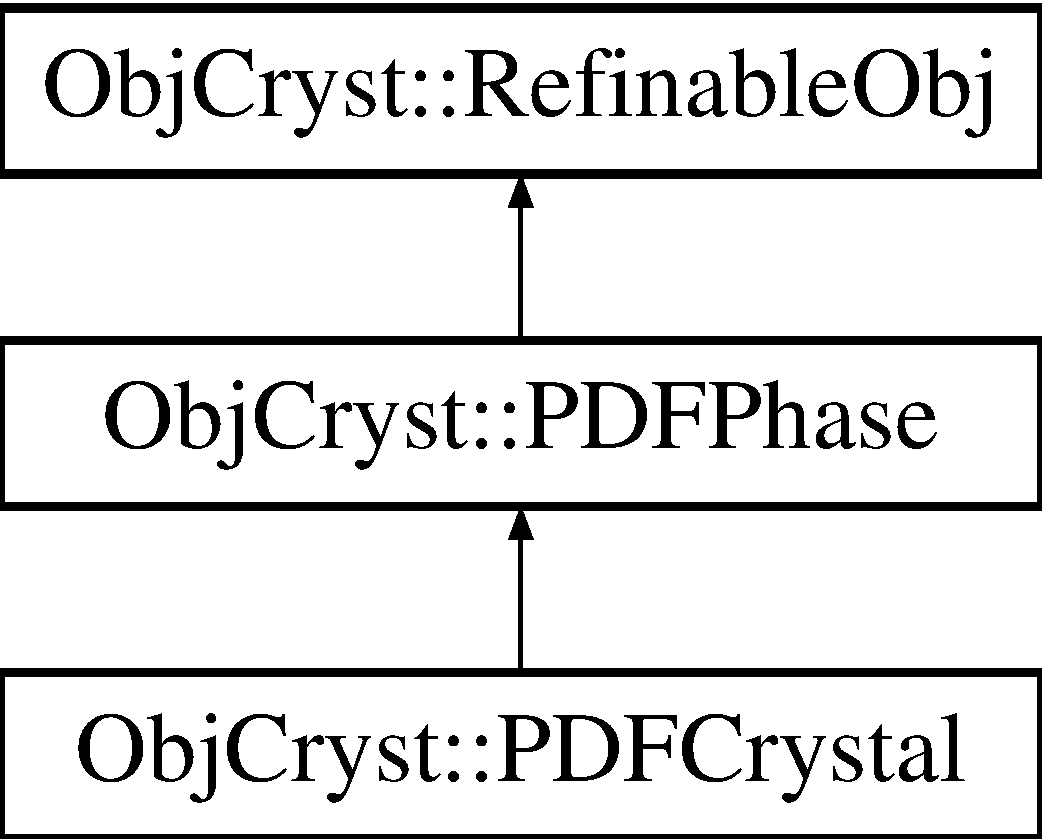
\includegraphics[height=3.000000cm]{a00065}
\end{center}
\end{figure}
\subsubsection*{\-Public \-Member \-Functions}
\begin{DoxyCompactItemize}
\item 
{\bfseries \-Powder\-Pattern\-Component} (const {\bf \-Powder\-Pattern\-Component} \&)\label{a00065_a10afd347f725df06fa8fabf94ee9c90f}

\item 
virtual const string \& {\bf \-Get\-Class\-Name} () const 
\begin{DoxyCompactList}\small\item\em \-Name for this class (\char`\"{}\-Refinable\-Obj\char`\"{}, \char`\"{}\-Crystal\char`\"{},...). \end{DoxyCompactList}\item 
const {\bf \-Powder\-Pattern} \& {\bf \-Get\-Parent\-Powder\-Pattern} () const 
\begin{DoxyCompactList}\small\item\em \-Get the \doxyref{\-Powder\-Pattern}{p.}{a00062} object which uses this component. \end{DoxyCompactList}\item 
{\bf \-Powder\-Pattern} \& {\bf \-Get\-Parent\-Powder\-Pattern} ()
\begin{DoxyCompactList}\small\item\em \-Get the \doxyref{\-Powder\-Pattern}{p.}{a00062} object which uses this component. \end{DoxyCompactList}\item 
virtual void {\bf \-Set\-Parent\-Powder\-Pattern} ({\bf \-Powder\-Pattern} \&)=0
\begin{DoxyCompactList}\small\item\em \-Set the \doxyref{\-Powder\-Pattern}{p.}{a00062} object which uses this component. \end{DoxyCompactList}\item 
virtual const \-Cryst\-Vector\-\_\-\-R\-E\-A\-L \& {\bf \-Get\-Powder\-Pattern\-Calc} () const =0
\begin{DoxyCompactList}\small\item\em \-Get the calculated powder pattern for this component. \end{DoxyCompactList}\item 
virtual pair$<$ const \*
\-Cryst\-Vector\-\_\-\-R\-E\-A\-L $\ast$, const \*
{\bf \-Refinable\-Obj\-Clock} $\ast$ $>$ {\bf \-Get\-Powder\-Pattern\-Integrated\-Calc} () const =0
\begin{DoxyCompactList}\small\item\em \-Get the integrated values of the powder pattern. \end{DoxyCompactList}\item 
bool {\bf \-Is\-Scalable} () const 
\begin{DoxyCompactList}\small\item\em \-Is this component scalable ? \end{DoxyCompactList}\item 
virtual const \-Cryst\-Vector\-\_\-\-R\-E\-A\-L \& {\bf \-Get\-Powder\-Pattern\-Calc\-Variance} () const =0
\begin{DoxyCompactList}\small\item\em \-Get the variance associated to each point of the calculated powder pattern, for this component. \end{DoxyCompactList}\item 
virtual pair$<$ const \*
\-Cryst\-Vector\-\_\-\-R\-E\-A\-L $\ast$, const \*
{\bf \-Refinable\-Obj\-Clock} $\ast$ $>$ {\bf \-Get\-Powder\-Pattern\-Integrated\-Calc\-Variance} () const =0
\begin{DoxyCompactList}\small\item\em \-Get the variance associated to each point of the calculated powder pattern, for this component (integrated version). \end{DoxyCompactList}\item 
virtual bool {\bf \-Has\-Powder\-Pattern\-Calc\-Variance} () const =0\label{a00065_a773d077df9d066f3d15631ec84ca15fd}

\begin{DoxyCompactList}\small\item\em \-Does this component have a variance associated with each calculated point ? i.\-e., do we use maximum likelihood to take into account incomplete models ? \end{DoxyCompactList}\item 
const {\bf \-Refinable\-Obj\-Clock} \& {\bf \-Get\-Clock\-Powder\-Pattern\-Calc} () const \label{a00065_a179247c07e05dcaa468ce149d9cd5a06}

\begin{DoxyCompactList}\small\item\em \-Last time the powder pattern was calculated. \end{DoxyCompactList}\item 
const list$<$ pair$<$ const \-R\-E\-A\-L,const \*
string $>$ $>$ \& {\bf \-Get\-Pattern\-Label\-List} () const 
\begin{DoxyCompactList}\small\item\em \-Get a list of labels for the pattern (usually reflection indexes). \end{DoxyCompactList}\end{DoxyCompactItemize}
\subsubsection*{\-Protected \-Member \-Functions}
\begin{DoxyCompactItemize}
\item 
const {\bf \-Refinable\-Obj\-Clock} \& {\bf \-Get\-Clock\-Powder\-Pattern\-Calc\-Variance} () const \label{a00065_a96109dc93d23fdc2ec87b25e42254ae0}

\begin{DoxyCompactList}\small\item\em \-Last time the variance on the pattern was actually calculated. \end{DoxyCompactList}\item 
virtual void {\bf \-Calc\-Powder\-Pattern} () const =0
\begin{DoxyCompactList}\small\item\em \-Calc the powder pattern. \end{DoxyCompactList}\item 
virtual void {\bf \-Calc\-Powder\-Pattern\-Integrated} () const =0
\begin{DoxyCompactList}\small\item\em \-Calc the integrated powder pattern. \end{DoxyCompactList}\item 
virtual const \-Cryst\-Vector\-\_\-long \& {\bf \-Get\-Bragg\-Limits} () const =0
\begin{DoxyCompactList}\small\item\em \-Get the pixel positions separating the integration intervals around reflections. \end{DoxyCompactList}\item 
const {\bf \-Refinable\-Obj\-Clock} \& {\bf \-Get\-Clock\-Bragg\-Limits} () const \label{a00065_a3743a5978a853dacabb004096519b35f}

\begin{DoxyCompactList}\small\item\em \-Get last time the \-Bragg \-Limits were changed. \end{DoxyCompactList}\item 
virtual void {\bf \-Set\-Max\-Sin\-Theta\-Ov\-Lambda} (const \-R\-E\-A\-L max)=0
\begin{DoxyCompactList}\small\item\em \-Set the maximum value for sin(theta)/lambda. \end{DoxyCompactList}\item 
virtual void {\bf \-Prepare} ()=0
\end{DoxyCompactItemize}
\subsubsection*{\-Protected \-Attributes}
\begin{DoxyCompactItemize}
\item 
\-Cryst\-Vector\-\_\-\-R\-E\-A\-L {\bf m\-Powder\-Pattern\-Calc}
\begin{DoxyCompactList}\small\item\em \-The calculated component of a powder pattern. \end{DoxyCompactList}\item 
\-Cryst\-Vector\-\_\-\-R\-E\-A\-L {\bf m\-Powder\-Pattern\-Integrated\-Calc}\label{a00065_a86c152ac7f6fca46572986ea99686ae0}

\begin{DoxyCompactList}\small\item\em \-The calculated powder pattern, integrated. \end{DoxyCompactList}\item 
\-Cryst\-Vector\-\_\-\-R\-E\-A\-L {\bf m\-Powder\-Pattern\-Calc\-Variance}\label{a00065_a01a50aa4e4114acc999676cd8069d426}

\begin{DoxyCompactList}\small\item\em \-The variance associated to each point of the calculated powder pattern. \end{DoxyCompactList}\item 
\-Cryst\-Vector\-\_\-\-R\-E\-A\-L {\bf m\-Powder\-Pattern\-Integrated\-Calc\-Variance}\label{a00065_aeaeac00300d33fa5d9ebae323143c6e2}

\begin{DoxyCompactList}\small\item\em \-The variance associated to each point of the calculated powder pattern, integrated. \end{DoxyCompactList}\item 
\-Cryst\-Vector\-\_\-long {\bf m\-Integrated\-Refl\-Limits}\label{a00065_ad0441f62b3b16e18f7cbdda6d89432cb}

\begin{DoxyCompactList}\small\item\em \-Interval limits around each reflection, for integrated \-R-\/factors. \end{DoxyCompactList}\item 
bool {\bf m\-Is\-Scalable}\label{a00065_aa1729b95ee7b6fbdc3e6aa7a9ca94aad}

\begin{DoxyCompactList}\small\item\em \-Scalable ? (crystal phase = scalable, background= not scalable) \end{DoxyCompactList}\item 
{\bf \-Refinable\-Obj\-Clock} {\bf m\-Clock\-Powder\-Pattern\-Calc}\label{a00065_aa64deb96cf54c504d9a24cdf209e9e0e}

\begin{DoxyCompactList}\small\item\em \-When was the powder pattern last computed ? \end{DoxyCompactList}\item 
{\bf \-Refinable\-Obj\-Clock} {\bf m\-Clock\-Powder\-Pattern\-Integrated\-Calc}\label{a00065_adc8435a9476962ad2876a8cfbee5cde5}

\begin{DoxyCompactList}\small\item\em \-When was the 'integrated' powder pattern last computed ? \end{DoxyCompactList}\item 
{\bf \-Refinable\-Obj\-Clock} {\bf m\-Clock\-Powder\-Pattern\-Variance\-Calc}\label{a00065_a503f89c2087ebd815e5df69961efb148}

\begin{DoxyCompactList}\small\item\em \-When was the powder pattern variance last computed ? \end{DoxyCompactList}\item 
{\bf \-Refinable\-Obj\-Clock} {\bf m\-Clock\-Powder\-Pattern\-Integrated\-Variance\-Calc}\label{a00065_a4f1cc991dadf2cecfbd758c91b9cbd78}

\begin{DoxyCompactList}\small\item\em \-When was the 'integrated' powder pattern variance last computed ? \end{DoxyCompactList}\item 
{\bf \-Powder\-Pattern} $\ast$ {\bf mp\-Parent\-Powder\-Pattern}\label{a00065_ad565327e0f1e6af053d0766c39ced8a0}

\begin{DoxyCompactList}\small\item\em \-The \doxyref{\-Powder\-Pattern}{p.}{a00062} object in which this component is included. \end{DoxyCompactList}\item 
{\bf \-Refinable\-Obj\-Clock} {\bf m\-Clock\-Bragg\-Limits}\label{a00065_a7320d473c830fda04684c01a9cd1f5cb}

\begin{DoxyCompactList}\small\item\em \-Get last time the \-Bragg \-Limits were changed. \end{DoxyCompactList}\item 
list$<$ pair$<$ const \-R\-E\-A\-L,const \*
string $>$ $>$ {\bf mv\-Label}\label{a00065_abe173118c67113339887a9831ad3a10f}

\begin{DoxyCompactList}\small\item\em \-The labels associated to different points of the pattern. \end{DoxyCompactList}\end{DoxyCompactItemize}
\subsubsection*{\-Friends}
\begin{DoxyCompactItemize}
\item 
class {\bfseries \-Powder\-Pattern}\label{a00065_a7b7565a5c419f2d4753446ff094a44cb}

\end{DoxyCompactItemize}


\subsubsection{\-Detailed \-Description}
\-Generic class to compute components (eg the contribution of a given phase, or background) of a powder pattern. 

\-This is an abstract base class.

\-Most functions are protected, only to be accessed, internally or from the friend class \doxyref{\-Powder\-Pattern}{p.}{a00062}. 

\subsubsection{\-Member \-Function \-Documentation}
\index{\-Obj\-Cryst\-::\-Powder\-Pattern\-Component@{\-Obj\-Cryst\-::\-Powder\-Pattern\-Component}!\-Calc\-Powder\-Pattern@{\-Calc\-Powder\-Pattern}}
\index{\-Calc\-Powder\-Pattern@{\-Calc\-Powder\-Pattern}!ObjCryst::PowderPatternComponent@{\-Obj\-Cryst\-::\-Powder\-Pattern\-Component}}
\paragraph[{\-Calc\-Powder\-Pattern}]{\setlength{\rightskip}{0pt plus 5cm}virtual void {\bf \-Obj\-Cryst\-::\-Powder\-Pattern\-Component\-::\-Calc\-Powder\-Pattern} (
\begin{DoxyParamCaption}
{}
\end{DoxyParamCaption}
) const\hspace{0.3cm}{\ttfamily  [protected, pure virtual]}}\label{a00065_a8417ecb93009a9b7b9fccf074a9438d9}


\-Calc the powder pattern. 

\-As always, recomputation is only done if necessary (ie if a parameter has changed since the last computation) 

\-Implemented in {\bf \-Obj\-Cryst\-::\-Powder\-Pattern\-Diffraction} \doxyref{}{p.}{a00066_a1f37b1e47c8bef989931fac08cf18849}, and {\bf \-Obj\-Cryst\-::\-Powder\-Pattern\-Background} \doxyref{}{p.}{a00063_a563a5021d4d1dbbf7d5cec58f524c60a}.

\index{\-Obj\-Cryst\-::\-Powder\-Pattern\-Component@{\-Obj\-Cryst\-::\-Powder\-Pattern\-Component}!\-Calc\-Powder\-Pattern\-Integrated@{\-Calc\-Powder\-Pattern\-Integrated}}
\index{\-Calc\-Powder\-Pattern\-Integrated@{\-Calc\-Powder\-Pattern\-Integrated}!ObjCryst::PowderPatternComponent@{\-Obj\-Cryst\-::\-Powder\-Pattern\-Component}}
\paragraph[{\-Calc\-Powder\-Pattern\-Integrated}]{\setlength{\rightskip}{0pt plus 5cm}virtual void {\bf \-Obj\-Cryst\-::\-Powder\-Pattern\-Component\-::\-Calc\-Powder\-Pattern\-Integrated} (
\begin{DoxyParamCaption}
{}
\end{DoxyParamCaption}
) const\hspace{0.3cm}{\ttfamily  [protected, pure virtual]}}\label{a00065_a24c4fb58e500cd669f3298475a31f72f}


\-Calc the integrated powder pattern. 

\-This should be optimized so that the full powder pattern is not explicitely computed. 

\-Implemented in {\bf \-Obj\-Cryst\-::\-Powder\-Pattern\-Diffraction} \doxyref{}{p.}{a00066_ae9e715bb230da8a3683adfee296288ad}, and {\bf \-Obj\-Cryst\-::\-Powder\-Pattern\-Background} \doxyref{}{p.}{a00063_af486465f3fa318d9d7737fb1347d0649}.

\index{\-Obj\-Cryst\-::\-Powder\-Pattern\-Component@{\-Obj\-Cryst\-::\-Powder\-Pattern\-Component}!\-Get\-Bragg\-Limits@{\-Get\-Bragg\-Limits}}
\index{\-Get\-Bragg\-Limits@{\-Get\-Bragg\-Limits}!ObjCryst::PowderPatternComponent@{\-Obj\-Cryst\-::\-Powder\-Pattern\-Component}}
\paragraph[{\-Get\-Bragg\-Limits}]{\setlength{\rightskip}{0pt plus 5cm}virtual const \-Cryst\-Vector\-\_\-long\& {\bf \-Obj\-Cryst\-::\-Powder\-Pattern\-Component\-::\-Get\-Bragg\-Limits} (
\begin{DoxyParamCaption}
{}
\end{DoxyParamCaption}
) const\hspace{0.3cm}{\ttfamily  [protected, pure virtual]}}\label{a00065_a727488f859528b0a9b5da47973804e01}


\-Get the pixel positions separating the integration intervals around reflections. 

\begin{DoxyReturn}{\-Returns}
\-: an array with the pixel positions, empty if this component has no peaks. \-The positions should be in increasing order, but could go beyond the pattern limits. 
\end{DoxyReturn}


\-Implemented in {\bf \-Obj\-Cryst\-::\-Powder\-Pattern\-Diffraction} \doxyref{}{p.}{a00066_ab9e21f6f16d77e96e4b5bed47db82dca}, and {\bf \-Obj\-Cryst\-::\-Powder\-Pattern\-Background} \doxyref{}{p.}{a00063_a348238a43c30b1601eaa1c30503b56e2}.

\index{\-Obj\-Cryst\-::\-Powder\-Pattern\-Component@{\-Obj\-Cryst\-::\-Powder\-Pattern\-Component}!\-Get\-Class\-Name@{\-Get\-Class\-Name}}
\index{\-Get\-Class\-Name@{\-Get\-Class\-Name}!ObjCryst::PowderPatternComponent@{\-Obj\-Cryst\-::\-Powder\-Pattern\-Component}}
\paragraph[{\-Get\-Class\-Name}]{\setlength{\rightskip}{0pt plus 5cm}virtual const string\& {\bf \-Obj\-Cryst\-::\-Powder\-Pattern\-Component\-::\-Get\-Class\-Name} (
\begin{DoxyParamCaption}
{}
\end{DoxyParamCaption}
) const\hspace{0.3cm}{\ttfamily  [virtual]}}\label{a00065_a5e797476d8d76ef797e1e8b51db9e8fb}


\-Name for this class (\char`\"{}\-Refinable\-Obj\char`\"{}, \char`\"{}\-Crystal\char`\"{},...). 

\-This is only useful to distinguish different classes when picking up objects from the \doxyref{\-Refinable\-Obj}{p.}{a00071} \-Global \-Registry 

\-Reimplemented from {\bf \-Obj\-Cryst\-::\-Refinable\-Obj} \doxyref{}{p.}{a00071_a62968d90a7a3080738b363934616c019}.



\-Reimplemented in {\bf \-Obj\-Cryst\-::\-Powder\-Pattern\-Diffraction} \doxyref{}{p.}{a00066_a74b02e35219c6bc18521e66719778881}, and {\bf \-Obj\-Cryst\-::\-Powder\-Pattern\-Background} \doxyref{}{p.}{a00063_afae084513270b7adf50954bec4037380}.

\index{\-Obj\-Cryst\-::\-Powder\-Pattern\-Component@{\-Obj\-Cryst\-::\-Powder\-Pattern\-Component}!\-Get\-Parent\-Powder\-Pattern@{\-Get\-Parent\-Powder\-Pattern}}
\index{\-Get\-Parent\-Powder\-Pattern@{\-Get\-Parent\-Powder\-Pattern}!ObjCryst::PowderPatternComponent@{\-Obj\-Cryst\-::\-Powder\-Pattern\-Component}}
\paragraph[{\-Get\-Parent\-Powder\-Pattern}]{\setlength{\rightskip}{0pt plus 5cm}const {\bf \-Powder\-Pattern}\& {\bf \-Obj\-Cryst\-::\-Powder\-Pattern\-Component\-::\-Get\-Parent\-Powder\-Pattern} (
\begin{DoxyParamCaption}
{}
\end{DoxyParamCaption}
) const}\label{a00065_a86b0e6ff842608be85b3465f4c179434}


\-Get the \doxyref{\-Powder\-Pattern}{p.}{a00062} object which uses this component. 

\-This allows to know the observed powder pattern to evaluate the background. \index{\-Obj\-Cryst\-::\-Powder\-Pattern\-Component@{\-Obj\-Cryst\-::\-Powder\-Pattern\-Component}!\-Get\-Parent\-Powder\-Pattern@{\-Get\-Parent\-Powder\-Pattern}}
\index{\-Get\-Parent\-Powder\-Pattern@{\-Get\-Parent\-Powder\-Pattern}!ObjCryst::PowderPatternComponent@{\-Obj\-Cryst\-::\-Powder\-Pattern\-Component}}
\paragraph[{\-Get\-Parent\-Powder\-Pattern}]{\setlength{\rightskip}{0pt plus 5cm}{\bf \-Powder\-Pattern}\& {\bf \-Obj\-Cryst\-::\-Powder\-Pattern\-Component\-::\-Get\-Parent\-Powder\-Pattern} (
\begin{DoxyParamCaption}
{}
\end{DoxyParamCaption}
)}\label{a00065_aa2b7cef2cb0c00f17b87efefa26448fd}


\-Get the \doxyref{\-Powder\-Pattern}{p.}{a00062} object which uses this component. 

\-This allows to know the observed powder pattern to evaluate the background. \index{\-Obj\-Cryst\-::\-Powder\-Pattern\-Component@{\-Obj\-Cryst\-::\-Powder\-Pattern\-Component}!\-Get\-Pattern\-Label\-List@{\-Get\-Pattern\-Label\-List}}
\index{\-Get\-Pattern\-Label\-List@{\-Get\-Pattern\-Label\-List}!ObjCryst::PowderPatternComponent@{\-Obj\-Cryst\-::\-Powder\-Pattern\-Component}}
\paragraph[{\-Get\-Pattern\-Label\-List}]{\setlength{\rightskip}{0pt plus 5cm}const list$<$pair$<$const \-R\-E\-A\-L ,const string $>$ $>$\& {\bf \-Obj\-Cryst\-::\-Powder\-Pattern\-Component\-::\-Get\-Pattern\-Label\-List} (
\begin{DoxyParamCaption}
{}
\end{DoxyParamCaption}
) const}\label{a00065_a9307408216499bf327b919fd0a0141bf}


\-Get a list of labels for the pattern (usually reflection indexes). 

\-This returns the list generated during the last computation of the powder pattern. \index{\-Obj\-Cryst\-::\-Powder\-Pattern\-Component@{\-Obj\-Cryst\-::\-Powder\-Pattern\-Component}!\-Get\-Powder\-Pattern\-Calc@{\-Get\-Powder\-Pattern\-Calc}}
\index{\-Get\-Powder\-Pattern\-Calc@{\-Get\-Powder\-Pattern\-Calc}!ObjCryst::PowderPatternComponent@{\-Obj\-Cryst\-::\-Powder\-Pattern\-Component}}
\paragraph[{\-Get\-Powder\-Pattern\-Calc}]{\setlength{\rightskip}{0pt plus 5cm}virtual const \-Cryst\-Vector\-\_\-\-R\-E\-A\-L\& {\bf \-Obj\-Cryst\-::\-Powder\-Pattern\-Component\-::\-Get\-Powder\-Pattern\-Calc} (
\begin{DoxyParamCaption}
{}
\end{DoxyParamCaption}
) const\hspace{0.3cm}{\ttfamily  [pure virtual]}}\label{a00065_a45258e9f9b44ff019bf53aa3dfb1a305}


\-Get the calculated powder pattern for this component. 

\-Note that the pattern is {\itshape not\/} scaled. 

\-Implemented in {\bf \-Obj\-Cryst\-::\-Powder\-Pattern\-Diffraction} \doxyref{}{p.}{a00066_a8003dc9bbaf67b5d95e443c20166b742}, and {\bf \-Obj\-Cryst\-::\-Powder\-Pattern\-Background} \doxyref{}{p.}{a00063_adb37c0a9b8e41e6dc11e6a9718c89bf5}.

\index{\-Obj\-Cryst\-::\-Powder\-Pattern\-Component@{\-Obj\-Cryst\-::\-Powder\-Pattern\-Component}!\-Get\-Powder\-Pattern\-Calc\-Variance@{\-Get\-Powder\-Pattern\-Calc\-Variance}}
\index{\-Get\-Powder\-Pattern\-Calc\-Variance@{\-Get\-Powder\-Pattern\-Calc\-Variance}!ObjCryst::PowderPatternComponent@{\-Obj\-Cryst\-::\-Powder\-Pattern\-Component}}
\paragraph[{\-Get\-Powder\-Pattern\-Calc\-Variance}]{\setlength{\rightskip}{0pt plus 5cm}virtual const \-Cryst\-Vector\-\_\-\-R\-E\-A\-L\& {\bf \-Obj\-Cryst\-::\-Powder\-Pattern\-Component\-::\-Get\-Powder\-Pattern\-Calc\-Variance} (
\begin{DoxyParamCaption}
{}
\end{DoxyParamCaption}
) const\hspace{0.3cm}{\ttfamily  [pure virtual]}}\label{a00065_ad67b39669fd0d336b01937ee81a59ddc}


\-Get the variance associated to each point of the calculated powder pattern, for this component. 

\begin{DoxyWarning}{\-Warning}
\-: this is experimental, with the aim of using \-Maximum \-Likelihood to improve structure determination. 
\end{DoxyWarning}


\-Implemented in {\bf \-Obj\-Cryst\-::\-Powder\-Pattern\-Diffraction} \doxyref{}{p.}{a00066_a664e1f47391720d06ffaa2b10b0aaf49}, and {\bf \-Obj\-Cryst\-::\-Powder\-Pattern\-Background} \doxyref{}{p.}{a00063_a871e01608feb73589bb27f4375194630}.

\index{\-Obj\-Cryst\-::\-Powder\-Pattern\-Component@{\-Obj\-Cryst\-::\-Powder\-Pattern\-Component}!\-Get\-Powder\-Pattern\-Integrated\-Calc@{\-Get\-Powder\-Pattern\-Integrated\-Calc}}
\index{\-Get\-Powder\-Pattern\-Integrated\-Calc@{\-Get\-Powder\-Pattern\-Integrated\-Calc}!ObjCryst::PowderPatternComponent@{\-Obj\-Cryst\-::\-Powder\-Pattern\-Component}}
\paragraph[{\-Get\-Powder\-Pattern\-Integrated\-Calc}]{\setlength{\rightskip}{0pt plus 5cm}virtual pair$<$const \-Cryst\-Vector\-\_\-\-R\-E\-A\-L$\ast$,const {\bf \-Refinable\-Obj\-Clock}$\ast$$>$ {\bf \-Obj\-Cryst\-::\-Powder\-Pattern\-Component\-::\-Get\-Powder\-Pattern\-Integrated\-Calc} (
\begin{DoxyParamCaption}
{}
\end{DoxyParamCaption}
) const\hspace{0.3cm}{\ttfamily  [pure virtual]}}\label{a00065_ac54b7ae5a177492de681afc2cbed72eb}


\-Get the integrated values of the powder pattern. 

\begin{DoxyNote}{\-Note}
\-: the integration intervals are those given by the parent \doxyref{\-Powder\-Pattern}{p.}{a00062}, so that all \doxyref{\-Powder\-Pattern\-Component}{p.}{a00065}'s intervals are taken into account
\end{DoxyNote}
\-This avoids explicitely calculating the full profile powder pattern. 

\-Implemented in {\bf \-Obj\-Cryst\-::\-Powder\-Pattern\-Diffraction} \doxyref{}{p.}{a00066_a2f2a745dcfa6cb7b7af4523b268827fe}, and {\bf \-Obj\-Cryst\-::\-Powder\-Pattern\-Background} \doxyref{}{p.}{a00063_a5bc997017cf1d95641b44021175c3dad}.

\index{\-Obj\-Cryst\-::\-Powder\-Pattern\-Component@{\-Obj\-Cryst\-::\-Powder\-Pattern\-Component}!\-Get\-Powder\-Pattern\-Integrated\-Calc\-Variance@{\-Get\-Powder\-Pattern\-Integrated\-Calc\-Variance}}
\index{\-Get\-Powder\-Pattern\-Integrated\-Calc\-Variance@{\-Get\-Powder\-Pattern\-Integrated\-Calc\-Variance}!ObjCryst::PowderPatternComponent@{\-Obj\-Cryst\-::\-Powder\-Pattern\-Component}}
\paragraph[{\-Get\-Powder\-Pattern\-Integrated\-Calc\-Variance}]{\setlength{\rightskip}{0pt plus 5cm}virtual pair$<$const \-Cryst\-Vector\-\_\-\-R\-E\-A\-L$\ast$,const {\bf \-Refinable\-Obj\-Clock}$\ast$$>$ {\bf \-Obj\-Cryst\-::\-Powder\-Pattern\-Component\-::\-Get\-Powder\-Pattern\-Integrated\-Calc\-Variance} (
\begin{DoxyParamCaption}
{}
\end{DoxyParamCaption}
) const\hspace{0.3cm}{\ttfamily  [pure virtual]}}\label{a00065_ae721bd290b50aa9503bac419616a21c6}


\-Get the variance associated to each point of the calculated powder pattern, for this component (integrated version). 

\begin{DoxyWarning}{\-Warning}
\-: this is experimental, with the aim of using \-Maximum \-Likelihood to improve structure determination. 
\end{DoxyWarning}


\-Implemented in {\bf \-Obj\-Cryst\-::\-Powder\-Pattern\-Diffraction} \doxyref{}{p.}{a00066_ae529ea1dab34388e88ba4a818ed48ca1}, and {\bf \-Obj\-Cryst\-::\-Powder\-Pattern\-Background} \doxyref{}{p.}{a00063_a48d8a351e2fcb8428a9af36c6a4fbf0f}.

\index{\-Obj\-Cryst\-::\-Powder\-Pattern\-Component@{\-Obj\-Cryst\-::\-Powder\-Pattern\-Component}!\-Is\-Scalable@{\-Is\-Scalable}}
\index{\-Is\-Scalable@{\-Is\-Scalable}!ObjCryst::PowderPatternComponent@{\-Obj\-Cryst\-::\-Powder\-Pattern\-Component}}
\paragraph[{\-Is\-Scalable}]{\setlength{\rightskip}{0pt plus 5cm}bool {\bf \-Obj\-Cryst\-::\-Powder\-Pattern\-Component\-::\-Is\-Scalable} (
\begin{DoxyParamCaption}
{}
\end{DoxyParamCaption}
) const}\label{a00065_aa0449b956187c242c3540a44e0a43e02}


\-Is this component scalable ? 

\-This is used by the \doxyref{\-Powder\-Pattern}{p.}{a00062} class, which fits all pattern components using scale factors. \-Some components may not need to be scaled\-: background components, which are assumed to be absolute. \index{\-Obj\-Cryst\-::\-Powder\-Pattern\-Component@{\-Obj\-Cryst\-::\-Powder\-Pattern\-Component}!\-Prepare@{\-Prepare}}
\index{\-Prepare@{\-Prepare}!ObjCryst::PowderPatternComponent@{\-Obj\-Cryst\-::\-Powder\-Pattern\-Component}}
\paragraph[{\-Prepare}]{\setlength{\rightskip}{0pt plus 5cm}virtual void {\bf \-Obj\-Cryst\-::\-Powder\-Pattern\-Component\-::\-Prepare} (
\begin{DoxyParamCaption}
{}
\end{DoxyParamCaption}
)\hspace{0.3cm}{\ttfamily  [protected, pure virtual]}}\label{a00065_a6a99877f0f9dec09fd5f596a7ddeb6f6}
\-This will be called by the parent \doxyref{\-Powder\-Pattern}{p.}{a00062} object, before calculating the first powder pattern. \-Or maybe it should be called automatically by the object itself... 

\-Reimplemented from {\bf \-Obj\-Cryst\-::\-Refinable\-Obj} \doxyref{}{p.}{a00071_a48d11671e7f8699f7bc24077585c5e0f}.



\-Implemented in {\bf \-Obj\-Cryst\-::\-Powder\-Pattern\-Diffraction} \doxyref{}{p.}{a00066_ae19852383674ae3ab673748a30a8432a}, and {\bf \-Obj\-Cryst\-::\-Powder\-Pattern\-Background} \doxyref{}{p.}{a00063_aac7d53c229cd59c2c9d4c5de539a60e1}.

\index{\-Obj\-Cryst\-::\-Powder\-Pattern\-Component@{\-Obj\-Cryst\-::\-Powder\-Pattern\-Component}!\-Set\-Max\-Sin\-Theta\-Ov\-Lambda@{\-Set\-Max\-Sin\-Theta\-Ov\-Lambda}}
\index{\-Set\-Max\-Sin\-Theta\-Ov\-Lambda@{\-Set\-Max\-Sin\-Theta\-Ov\-Lambda}!ObjCryst::PowderPatternComponent@{\-Obj\-Cryst\-::\-Powder\-Pattern\-Component}}
\paragraph[{\-Set\-Max\-Sin\-Theta\-Ov\-Lambda}]{\setlength{\rightskip}{0pt plus 5cm}virtual void {\bf \-Obj\-Cryst\-::\-Powder\-Pattern\-Component\-::\-Set\-Max\-Sin\-Theta\-Ov\-Lambda} (
\begin{DoxyParamCaption}
\item[{const \-R\-E\-A\-L}]{max}
\end{DoxyParamCaption}
)\hspace{0.3cm}{\ttfamily  [protected, pure virtual]}}\label{a00065_a4731b5a64ee9aab6779e2ef323242fe5}


\-Set the maximum value for sin(theta)/lambda. 

\-All data above still exist but are ignored for all calculations. 

\-Implemented in {\bf \-Obj\-Cryst\-::\-Powder\-Pattern\-Diffraction} \doxyref{}{p.}{a00066_a699af7ea523fca128032384b548ceef1}, and {\bf \-Obj\-Cryst\-::\-Powder\-Pattern\-Background} \doxyref{}{p.}{a00063_a6c6c5f75dc132609ba822337123edd1d}.

\index{\-Obj\-Cryst\-::\-Powder\-Pattern\-Component@{\-Obj\-Cryst\-::\-Powder\-Pattern\-Component}!\-Set\-Parent\-Powder\-Pattern@{\-Set\-Parent\-Powder\-Pattern}}
\index{\-Set\-Parent\-Powder\-Pattern@{\-Set\-Parent\-Powder\-Pattern}!ObjCryst::PowderPatternComponent@{\-Obj\-Cryst\-::\-Powder\-Pattern\-Component}}
\paragraph[{\-Set\-Parent\-Powder\-Pattern}]{\setlength{\rightskip}{0pt plus 5cm}virtual void {\bf \-Obj\-Cryst\-::\-Powder\-Pattern\-Component\-::\-Set\-Parent\-Powder\-Pattern} (
\begin{DoxyParamCaption}
\item[{{\bf \-Powder\-Pattern} \&}]{}
\end{DoxyParamCaption}
)\hspace{0.3cm}{\ttfamily  [pure virtual]}}\label{a00065_a6b3dc911118c280dbbdcb7fb97acf980}


\-Set the \doxyref{\-Powder\-Pattern}{p.}{a00062} object which uses this component. 

\-This sets all necessary pattern parameters (2theta/tof range, wavelength, radiation type...) accordingly. 

\-Implemented in {\bf \-Obj\-Cryst\-::\-Powder\-Pattern\-Diffraction} \doxyref{}{p.}{a00066_ab67953ad7f27c37334a6b557c2da1d73}, and {\bf \-Obj\-Cryst\-::\-Powder\-Pattern\-Background} \doxyref{}{p.}{a00063_a02032467fb6485e05f0a1bbf74133833}.



\subsubsection{\-Member \-Data \-Documentation}
\index{\-Obj\-Cryst\-::\-Powder\-Pattern\-Component@{\-Obj\-Cryst\-::\-Powder\-Pattern\-Component}!m\-Powder\-Pattern\-Calc@{m\-Powder\-Pattern\-Calc}}
\index{m\-Powder\-Pattern\-Calc@{m\-Powder\-Pattern\-Calc}!ObjCryst::PowderPatternComponent@{\-Obj\-Cryst\-::\-Powder\-Pattern\-Component}}
\paragraph[{m\-Powder\-Pattern\-Calc}]{\setlength{\rightskip}{0pt plus 5cm}\-Cryst\-Vector\-\_\-\-R\-E\-A\-L {\bf \-Obj\-Cryst\-::\-Powder\-Pattern\-Component\-::m\-Powder\-Pattern\-Calc}\hspace{0.3cm}{\ttfamily  [mutable, protected]}}\label{a00065_ae6e41d0a85e00cdf0a7d52f74dc20d4a}


\-The calculated component of a powder pattern. 

\-It is mutable since it is completely defined by other parameters (eg it is not an 'independent parameter') 

\-The documentation for this class was generated from the following file\-:\begin{DoxyCompactItemize}
\item 
\-Powder\-Pattern.\-h\end{DoxyCompactItemize}

\subsection{ObjCryst::PowderSlitApertureCorr Class Reference}
\label{a00066}\index{ObjCryst::PowderSlitApertureCorr@{ObjCryst::PowderSlitApertureCorr}}


Slit aperture correction (for powder).  
Inheritance diagram for ObjCryst::PowderSlitApertureCorr::\begin{figure}[H]
\begin{center}
\leavevmode
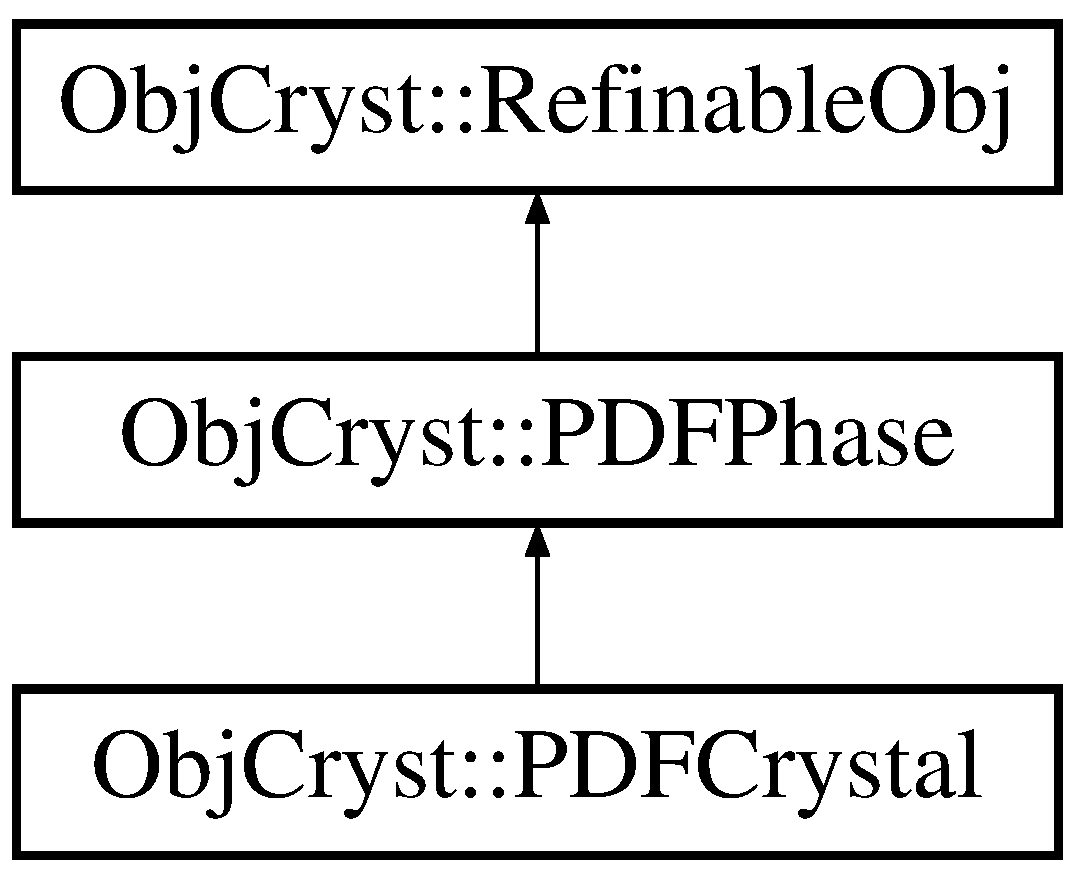
\includegraphics[height=2cm]{a00066}
\end{center}
\end{figure}
\subsubsection*{Public Member Functions}
\begin{DoxyCompactItemize}
\item 
{\bfseries PowderSlitApertureCorr} (const {\bf ScatteringData} \&data)\label{a00066_a8c7814fd23c9e2fe96a904ea41137caf}

\item 
virtual const string \& {\bf GetName} () const \label{a00066_a395cb337777d1c3fdd283f03c9a06e27}

\begin{DoxyCompactList}\small\item\em Get the name of this object. \item\end{DoxyCompactList}\item 
virtual const string \& {\bf GetClassName} () const \label{a00066_a36c1dd123d3f951ba140796f47a68fbb}

\begin{DoxyCompactList}\small\item\em Get the name of the class. \item\end{DoxyCompactList}\end{DoxyCompactItemize}
\subsubsection*{Protected Member Functions}
\begin{DoxyCompactItemize}
\item 
virtual void {\bf CalcCorr} () const \label{a00066_ae7b2fecebc30de79ccc54f5237ec67f7}

\begin{DoxyCompactList}\small\item\em Do the computation of corrected intensities. \item\end{DoxyCompactList}\end{DoxyCompactItemize}


\subsubsection{Detailed Description}
Slit aperture correction (for powder). This correction takes into account the fact that diffraction rings (cones) have a portion of the ring proportionnal to $ SlitAp = \frac{1}{\sin(\theta)} $ which falls into the detector (due to slits in the direction perpendicular to the incident beam/ detector plane). 

The documentation for this class was generated from the following file:\begin{DoxyCompactItemize}
\item 
ScatteringCorr.h\end{DoxyCompactItemize}

\subsection{\-Obj\-Cryst\-:\-:\-Powder\-Slit\-Aperture\-Corr \-Class \-Reference}
\label{a00067}\index{\-Obj\-Cryst\-::\-Powder\-Slit\-Aperture\-Corr@{\-Obj\-Cryst\-::\-Powder\-Slit\-Aperture\-Corr}}


\-Slit aperture correction (for powder)  


\-Inheritance diagram for \-Obj\-Cryst\-:\-:\-Powder\-Slit\-Aperture\-Corr\-:\begin{figure}[H]
\begin{center}
\leavevmode
\includegraphics[height=2.000000cm]{a00067}
\end{center}
\end{figure}
\subsubsection*{\-Public \-Member \-Functions}
\begin{DoxyCompactItemize}
\item 
{\bfseries \-Powder\-Slit\-Aperture\-Corr} (const {\bf \-Scattering\-Data} \&data)\label{a00067_a8c7814fd23c9e2fe96a904ea41137caf}

\item 
virtual const string \& {\bf \-Get\-Name} () const \label{a00067_a395cb337777d1c3fdd283f03c9a06e27}

\begin{DoxyCompactList}\small\item\em \-Get the name of this object. \end{DoxyCompactList}\item 
virtual const string \& {\bf \-Get\-Class\-Name} () const \label{a00067_a36c1dd123d3f951ba140796f47a68fbb}

\begin{DoxyCompactList}\small\item\em \-Get the name of the class. \end{DoxyCompactList}\end{DoxyCompactItemize}
\subsubsection*{\-Protected \-Member \-Functions}
\begin{DoxyCompactItemize}
\item 
virtual void {\bf \-Calc\-Corr} () const \label{a00067_ae7b2fecebc30de79ccc54f5237ec67f7}

\begin{DoxyCompactList}\small\item\em \-Do the computation of corrected intensities. \end{DoxyCompactList}\end{DoxyCompactItemize}


\subsubsection{\-Detailed \-Description}
\-Slit aperture correction (for powder) 

\-This correction takes into account the fact that diffraction rings (cones) have a portion of the ring proportionnal to $ SlitAp = \frac{1}{\sin(\theta)} $ which falls into the detector (due to slits in the direction perpendicular to the incident beam/ detector plane). 

\-The documentation for this class was generated from the following file\-:\begin{DoxyCompactItemize}
\item 
\-Scattering\-Corr.\-h\end{DoxyCompactItemize}

\subsection{Obj\-Cryst\-:\-:Polarization\-Corr Class Reference}
\label{a00068}\index{Obj\-Cryst\-::\-Polarization\-Corr@{Obj\-Cryst\-::\-Polarization\-Corr}}


Polarization Correction.  


Inheritance diagram for Obj\-Cryst\-:\-:Polarization\-Corr\-:\begin{figure}[H]
\begin{center}
\leavevmode
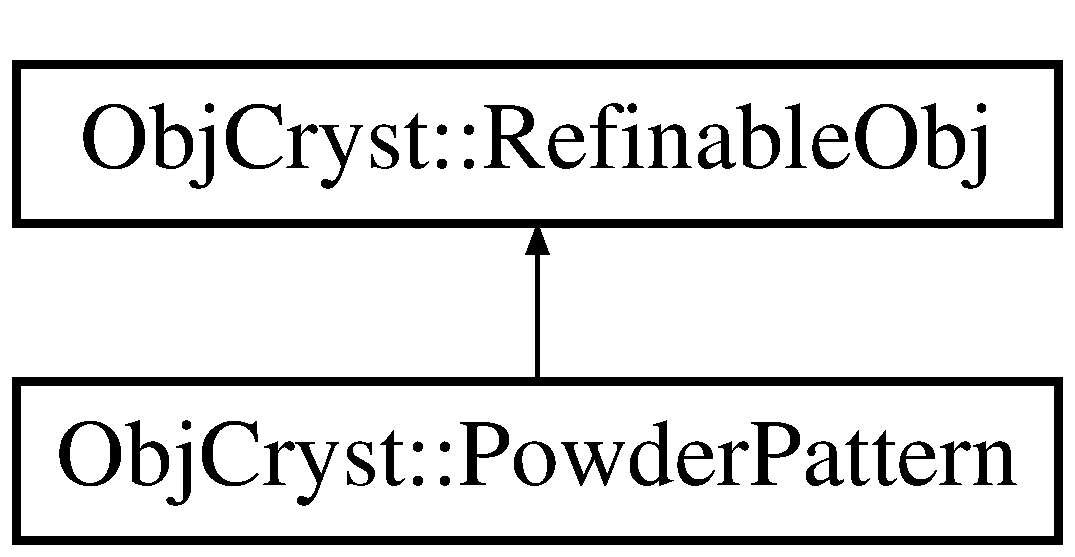
\includegraphics[height=2.000000cm]{a00068}
\end{center}
\end{figure}
\subsubsection*{Public Member Functions}
\begin{DoxyCompactItemize}
\item 
{\bfseries Polarization\-Corr} (const {\bf Scattering\-Data} \&data)\label{a00068_a2a4847d1595188d8023f20c9c9d0d4ce}

\item 
virtual const string \& {\bf Get\-Name} () const \label{a00068_a6bfca1f83186379f77e2ee2ef5e65ac5}

\begin{DoxyCompactList}\small\item\em Get the name of this object. \end{DoxyCompactList}\item 
virtual const string \& {\bf Get\-Class\-Name} () const \label{a00068_ae298bdf956280d610cc18aad4acb1af7}

\begin{DoxyCompactList}\small\item\em Get the name of the class. \end{DoxyCompactList}\end{DoxyCompactItemize}
\subsubsection*{Protected Member Functions}
\begin{DoxyCompactItemize}
\item 
virtual void {\bf Calc\-Corr} () const \label{a00068_a3030bd67935be0434c1cebfd385b82a2}

\begin{DoxyCompactList}\small\item\em Do the computation of corrected intensities. \end{DoxyCompactList}\end{DoxyCompactItemize}
\subsubsection*{Protected Attributes}
\begin{DoxyCompactItemize}
\item 
R\-E\-A\-L {\bfseries m\-Polar\-Afactor}\label{a00068_a8a0115cf6d539ede891056f94b6887cf}

\end{DoxyCompactItemize}


\subsubsection{Detailed Description}
Polarization Correction. 

So far, it only considers the correction for equatorial diffraction\-: $ P = \frac{1}{1+A}\left(1+A\cos^2(2\theta)\right) $ (Polarization factor), with $ A = \frac{1-f}{1+f} $, where f is the polarization rate of the incident beam in the plane which (i) includes the incident beam, and (ii) is perpendicular to the diffracting plane. For an X-\/\-Ray Tube without monochromator, A=1, and if there is a monochromator \-: $ A = \cos^2(2\theta_{mono}) $

Currently, the linear polarization factor is directly read from the radiation object, and the linear polarization (if any) is assumed to be perpendicular to the diffracting plane (standard synchrotron geometry).

\begin{DoxyRefDesc}{Todo}
\item[{\bf Todo}]\-: extend this to take into account other diffracting \& monochromatic geometries. \end{DoxyRefDesc}


The documentation for this class was generated from the following file\-:\begin{DoxyCompactItemize}
\item 
Scattering\-Corr.\-h\end{DoxyCompactItemize}

\subsection{Obj\-Cryst\-:\-:Powder\-Pattern\-Background Class Reference}
\label{a00069}\index{Obj\-Cryst\-::\-Powder\-Pattern\-Background@{Obj\-Cryst\-::\-Powder\-Pattern\-Background}}


Phase to compute a background contribution to a powder pattern using an interpolation.  


Inheritance diagram for Obj\-Cryst\-:\-:Powder\-Pattern\-Background\-:\begin{figure}[H]
\begin{center}
\leavevmode
\includegraphics[height=3.000000cm]{a00069}
\end{center}
\end{figure}
\subsubsection*{Public Member Functions}
\begin{DoxyCompactItemize}
\item 
{\bfseries Powder\-Pattern\-Background} (const {\bf Powder\-Pattern\-Background} \&)\label{a00069_a46496ee29e07d0c8949bfc45d77a4c3e}

\item 
virtual const string \& {\bf Get\-Class\-Name} () const 
\begin{DoxyCompactList}\small\item\em Name for this class (\char`\"{}\-Refinable\-Obj\char`\"{}, \char`\"{}\-Crystal\char`\"{},...). \end{DoxyCompactList}\item 
virtual void {\bf Set\-Parent\-Powder\-Pattern} ({\bf Powder\-Pattern} \&)
\begin{DoxyCompactList}\small\item\em Set the \doxyref{Powder\-Pattern}{p.}{a00068} object which uses this component. \end{DoxyCompactList}\item 
virtual const Cryst\-Vector\-\_\-\-R\-E\-A\-L \& {\bf Get\-Powder\-Pattern\-Calc} () const 
\begin{DoxyCompactList}\small\item\em Get the calculated powder pattern for this component. \end{DoxyCompactList}\item 
virtual pair$<$ const \\*
Cryst\-Vector\-\_\-\-R\-E\-A\-L $\ast$, const \\*
{\bf Refinable\-Obj\-Clock} $\ast$ $>$ {\bf Get\-Powder\-Pattern\-Integrated\-Calc} () const 
\begin{DoxyCompactList}\small\item\em Get the integrated values of the powder pattern. \end{DoxyCompactList}\item 
void {\bf Import\-User\-Background} (const string \&filename)\label{a00069_ae68fc3a9883ca45c81a22119c28d9379}

\begin{DoxyCompactList}\small\item\em Import background points from a file (with two columns 2theta (or tof), intensity) \end{DoxyCompactList}\item 
void {\bfseries Set\-Interp\-Points} (const Cryst\-Vector\-\_\-\-R\-E\-A\-L tth, const Cryst\-Vector\-\_\-\-R\-E\-A\-L backgd)\label{a00069_afda9ea065efbed3fcfc783060de9b415}

\item 
const std\-::pair$<$ const \\*
Cryst\-Vector\-\_\-\-R\-E\-A\-L $\ast$, const \\*
Cryst\-Vector\-\_\-\-R\-E\-A\-L $\ast$ $>$ {\bfseries Get\-Interp\-Points} () const \label{a00069_a09b8b88c54f8916cea09ffd93bb5c18d}

\item 
virtual void {\bf X\-M\-L\-Output} (ostream \&os, int indent=0) const 
\begin{DoxyCompactList}\small\item\em Output to stream in well-\/formed X\-M\-L. \end{DoxyCompactList}\item 
virtual void {\bf X\-M\-L\-Input} (istream \&is, const {\bf X\-M\-L\-Cryst\-Tag} \&tag)
\begin{DoxyCompactList}\small\item\em Input From stream. \end{DoxyCompactList}\item 
virtual void {\bf Get\-Gene\-Group} (const {\bf Refinable\-Obj} \&obj, Cryst\-Vector\-\_\-uint \&group\-Index, unsigned int \&first\-Group) const 
\begin{DoxyCompactList}\small\item\em Get the gene group assigned to each parameter. \end{DoxyCompactList}\item 
virtual void {\bf Begin\-Optimization} (const bool allow\-Approximations=false, const bool enable\-Restraints=false)
\begin{DoxyCompactList}\small\item\em This should be called by any optimization class at the begining of an optimization. \end{DoxyCompactList}\item 
virtual const Cryst\-Vector\-\_\-\-R\-E\-A\-L \& {\bf Get\-Powder\-Pattern\-Calc\-Variance} () const 
\begin{DoxyCompactList}\small\item\em Get the variance associated to each point of the calculated powder pattern, for this component. \end{DoxyCompactList}\item 
virtual pair$<$ const \\*
Cryst\-Vector\-\_\-\-R\-E\-A\-L $\ast$, const \\*
{\bf Refinable\-Obj\-Clock} $\ast$ $>$ {\bf Get\-Powder\-Pattern\-Integrated\-Calc\-Variance} () const 
\begin{DoxyCompactList}\small\item\em Get the variance associated to each point of the calculated powder pattern, for this component (integrated version). \end{DoxyCompactList}\item 
virtual bool {\bf Has\-Powder\-Pattern\-Calc\-Variance} () const \label{a00069_abae616675aa5f8cf66eb0b788aedb43d}

\begin{DoxyCompactList}\small\item\em Does this component have a variance associated with each calculated point ? i.\-e., do we use maximum likelihood to take into account incomplete models ? \end{DoxyCompactList}\item 
virtual void {\bf Tag\-New\-Best\-Config} () const 
\begin{DoxyCompactList}\small\item\em During a global optimization, tells the object that the current config is the latest \char`\"{}best\char`\"{} config. \end{DoxyCompactList}\item 
void {\bf Optimize\-Bayesian\-Background} ()
\begin{DoxyCompactList}\small\item\em Optimize the background using a Bayesian approach. \end{DoxyCompactList}\item 
void {\bf Fix\-Parameters\-Beyond\-Maxresolution} ({\bf Refinable\-Obj} \&obj)
\begin{DoxyCompactList}\small\item\em Fix parameters corresponding to points of the pattern that are not actually calculated. \end{DoxyCompactList}\end{DoxyCompactItemize}
\subsubsection*{Protected Member Functions}
\begin{DoxyCompactItemize}
\item 
virtual void {\bf Calc\-Powder\-Pattern} () const 
\begin{DoxyCompactList}\small\item\em Calc the powder pattern. \end{DoxyCompactList}\item 
virtual void {\bf Calc\-Powder\-Pattern\-Integrated} () const 
\begin{DoxyCompactList}\small\item\em Calc the integrated powder pattern. \end{DoxyCompactList}\item 
virtual void {\bf Prepare} ()
\item 
virtual const Cryst\-Vector\-\_\-long \& {\bf Get\-Bragg\-Limits} () const 
\begin{DoxyCompactList}\small\item\em Get the pixel positions separating the integration intervals around reflections. \end{DoxyCompactList}\item 
virtual void {\bf Set\-Max\-Sin\-Theta\-Ov\-Lambda} (const R\-E\-A\-L max)
\begin{DoxyCompactList}\small\item\em Set the maximum value for sin(theta)/lambda. \end{DoxyCompactList}\item 
void {\bfseries Init\-Ref\-Par\-List} ()\label{a00069_a5ec5ac4fd9ac7247fdb29c1b40e4369b}

\item 
void {\bfseries Init\-Options} ()\label{a00069_a9546d8c2c1de47d8eea570f20ab45bcb}

\item 
void {\bfseries Init\-Spline} () const \label{a00069_af795f71db9fadac9c6c142d9af6c8dcc}

\end{DoxyCompactItemize}
\subsubsection*{Protected Attributes}
\begin{DoxyCompactItemize}
\item 
int {\bf m\-Background\-Nb\-Point}\label{a00069_a1b41334ecbbbe337121f6041b7068e99}

\begin{DoxyCompactList}\small\item\em Number of fitting points for background. \end{DoxyCompactList}\item 
Cryst\-Vector\-\_\-\-R\-E\-A\-L {\bf m\-Background\-Interp\-Point\-X}\label{a00069_a68740ba9e8c4348e2a6b2d96024436eb}

\begin{DoxyCompactList}\small\item\em Vector of 2theta values for the fitting points of the background. \end{DoxyCompactList}\item 
Cryst\-Vector\-\_\-\-R\-E\-A\-L {\bf m\-Background\-Interp\-Point\-Intensity}\label{a00069_a942a33452d66e00cd155743a9c8c21e2}

\begin{DoxyCompactList}\small\item\em Values of background at interpolating points. \end{DoxyCompactList}\item 
Cryst\-Vector\-\_\-long {\bf m\-Point\-Order}
\begin{DoxyCompactList}\small\item\em Subscript of the points, sorted the correct order, taking into account the type of radiation (monochromatic/\-T\-O\-F). \end{DoxyCompactList}\item 
Cryst\-Vector\-\_\-\-R\-E\-A\-L {\bf mv\-Spline\-Pixel}
\begin{DoxyCompactList}\small\item\em Vector of pixel values between each interval, for faster \doxyref{Cubic\-Spline}{p.}{a00031} calculations. \end{DoxyCompactList}\item 
{\bf Cubic\-Spline} {\bf mv\-Spline}
\begin{DoxyCompactList}\small\item\em Spline used for interpolation. \end{DoxyCompactList}\item 
{\bf Refinable\-Obj\-Clock} {\bf m\-Clock\-Background\-Point}\label{a00069_ae26867d298bf99ee07d196b5636a144f}

\begin{DoxyCompactList}\small\item\em Modification of the interpolated points. \end{DoxyCompactList}\item 
{\bf Refinable\-Obj\-Clock} {\bf m\-Clock\-Spline}\label{a00069_af2988bbeae93a4ebe62161bfb136a859}

\begin{DoxyCompactList}\small\item\em Initialization of the spline. \end{DoxyCompactList}\item 
R\-E\-A\-L {\bf m\-Max\-Sin\-Theta\-Ov\-Lambda}
\begin{DoxyCompactList}\small\item\em Maximum sin(theta)/lambda for all calculations (10 by default). \end{DoxyCompactList}\item 
R\-E\-A\-L {\bf m\-Model\-Variance}\label{a00069_afb62b2f85e9bab627f14265830d1ff09}

\begin{DoxyCompactList}\small\item\em Constant error (sigma) on the calculated pattern, due to an incomplete model. \end{DoxyCompactList}\item 
{\bf Ref\-Obj\-Opt} {\bf m\-Interpolation\-Model}\label{a00069_a8dcbfb135b47ce820d7a6500818c84fd}

\begin{DoxyCompactList}\small\item\em Type of interpolation performed\-: linear or cubic spline. \end{DoxyCompactList}\end{DoxyCompactItemize}
\subsubsection*{Friends}
\begin{DoxyCompactItemize}
\item 
class {\bfseries Powder\-Pattern}\label{a00069_a7b7565a5c419f2d4753446ff094a44cb}

\end{DoxyCompactItemize}


\subsubsection{Detailed Description}
Phase to compute a background contribution to a powder pattern using an interpolation. 

Currently only linear interpolation is available. (in the works\-: cubic spline interpolation background) 

\subsubsection{Member Function Documentation}
\index{Obj\-Cryst\-::\-Powder\-Pattern\-Background@{Obj\-Cryst\-::\-Powder\-Pattern\-Background}!Begin\-Optimization@{Begin\-Optimization}}
\index{Begin\-Optimization@{Begin\-Optimization}!ObjCryst::PowderPatternBackground@{Obj\-Cryst\-::\-Powder\-Pattern\-Background}}
\paragraph[{Begin\-Optimization}]{\setlength{\rightskip}{0pt plus 5cm}virtual void Obj\-Cryst\-::\-Powder\-Pattern\-Background\-::\-Begin\-Optimization (
\begin{DoxyParamCaption}
\item[{const bool}]{allow\-Approximations = {\ttfamily false}, }
\item[{const bool}]{enable\-Restraints = {\ttfamily false}}
\end{DoxyParamCaption}
)\hspace{0.3cm}{\ttfamily [virtual]}}\label{a00069_ac9a022b49d583e8ae81e4d96e50cc9d8}


This should be called by any optimization class at the begining of an optimization. 

This will also check that everything is ready, eg call the \doxyref{Refinable\-Obj\-::\-Prepare()}{p.}{a00077_a48d11671e7f8699f7bc24077585c5e0f} function. This also affects all sub-\/objects. \begin{DoxyNote}{Note}
this may be called several time for some objects which are used by several other objects, or for nested optimizations (e.\-g. least-\/squares optimizations inside a global one).

\doxyref{End\-Optimization()}{p.}{a00077_ab0035f6164cb24ace67b51b11993a851} must be called at the end of the optimization, the same number of time \doxyref{Begin\-Optimization()}{p.}{a00069_ac9a022b49d583e8ae81e4d96e50cc9d8} was called !
\end{DoxyNote}

\begin{DoxyParams}{Parameters}
{\em allow\-Approximations} & if true, then the object can use faster but less precise functions during the optimization. This is useful for global optimization not using derivatives. \\
\hline
{\em enable\-Restraints\-:\textbackslash{}xrefitem} & deprecated 28. \\
\hline
\end{DoxyParams}


Reimplemented from {\bf Obj\-Cryst\-::\-Refinable\-Obj} \doxyref{}{p.}{a00077_ababd8f2916e41a20d2c1b21f6ffefe96}.

\index{Obj\-Cryst\-::\-Powder\-Pattern\-Background@{Obj\-Cryst\-::\-Powder\-Pattern\-Background}!Calc\-Powder\-Pattern@{Calc\-Powder\-Pattern}}
\index{Calc\-Powder\-Pattern@{Calc\-Powder\-Pattern}!ObjCryst::PowderPatternBackground@{Obj\-Cryst\-::\-Powder\-Pattern\-Background}}
\paragraph[{Calc\-Powder\-Pattern}]{\setlength{\rightskip}{0pt plus 5cm}virtual void Obj\-Cryst\-::\-Powder\-Pattern\-Background\-::\-Calc\-Powder\-Pattern (
\begin{DoxyParamCaption}
{}
\end{DoxyParamCaption}
) const\hspace{0.3cm}{\ttfamily [protected]}, {\ttfamily [virtual]}}\label{a00069_a563a5021d4d1dbbf7d5cec58f524c60a}


Calc the powder pattern. 

As always, recomputation is only done if necessary (ie if a parameter has changed since the last computation) 

Implements {\bf Obj\-Cryst\-::\-Powder\-Pattern\-Component} \doxyref{}{p.}{a00071_a8417ecb93009a9b7b9fccf074a9438d9}.

\index{Obj\-Cryst\-::\-Powder\-Pattern\-Background@{Obj\-Cryst\-::\-Powder\-Pattern\-Background}!Calc\-Powder\-Pattern\-Integrated@{Calc\-Powder\-Pattern\-Integrated}}
\index{Calc\-Powder\-Pattern\-Integrated@{Calc\-Powder\-Pattern\-Integrated}!ObjCryst::PowderPatternBackground@{Obj\-Cryst\-::\-Powder\-Pattern\-Background}}
\paragraph[{Calc\-Powder\-Pattern\-Integrated}]{\setlength{\rightskip}{0pt plus 5cm}virtual void Obj\-Cryst\-::\-Powder\-Pattern\-Background\-::\-Calc\-Powder\-Pattern\-Integrated (
\begin{DoxyParamCaption}
{}
\end{DoxyParamCaption}
) const\hspace{0.3cm}{\ttfamily [protected]}, {\ttfamily [virtual]}}\label{a00069_af486465f3fa318d9d7737fb1347d0649}


Calc the integrated powder pattern. 

This should be optimized so that the full powder pattern is not explicitely computed. 

Implements {\bf Obj\-Cryst\-::\-Powder\-Pattern\-Component} \doxyref{}{p.}{a00071_a24c4fb58e500cd669f3298475a31f72f}.

\index{Obj\-Cryst\-::\-Powder\-Pattern\-Background@{Obj\-Cryst\-::\-Powder\-Pattern\-Background}!Fix\-Parameters\-Beyond\-Maxresolution@{Fix\-Parameters\-Beyond\-Maxresolution}}
\index{Fix\-Parameters\-Beyond\-Maxresolution@{Fix\-Parameters\-Beyond\-Maxresolution}!ObjCryst::PowderPatternBackground@{Obj\-Cryst\-::\-Powder\-Pattern\-Background}}
\paragraph[{Fix\-Parameters\-Beyond\-Maxresolution}]{\setlength{\rightskip}{0pt plus 5cm}void Obj\-Cryst\-::\-Powder\-Pattern\-Background\-::\-Fix\-Parameters\-Beyond\-Maxresolution (
\begin{DoxyParamCaption}
\item[{{\bf Refinable\-Obj} \&}]{obj}
\end{DoxyParamCaption}
)}\label{a00069_a874e0bed05f17df53ad6ddd3df989dc9}


Fix parameters corresponding to points of the pattern that are not actually calculated. 

This is necessary for modelling using splines, to avoid divergence of interpolation points during least squares optimization.


\begin{DoxyParams}{Parameters}
{\em obj} & the object in which are parameters to be fixed. Normally this will be the \doxyref{Powder\-Pattern\-Background}{p.}{a00069} object itself, but it can also be the parameter list copied such as in a \doxyref{L\-S\-Q\-Num\-Obj}{p.}{a00045}. \\
\hline
\end{DoxyParams}
\index{Obj\-Cryst\-::\-Powder\-Pattern\-Background@{Obj\-Cryst\-::\-Powder\-Pattern\-Background}!Get\-Bragg\-Limits@{Get\-Bragg\-Limits}}
\index{Get\-Bragg\-Limits@{Get\-Bragg\-Limits}!ObjCryst::PowderPatternBackground@{Obj\-Cryst\-::\-Powder\-Pattern\-Background}}
\paragraph[{Get\-Bragg\-Limits}]{\setlength{\rightskip}{0pt plus 5cm}virtual const Cryst\-Vector\-\_\-long\& Obj\-Cryst\-::\-Powder\-Pattern\-Background\-::\-Get\-Bragg\-Limits (
\begin{DoxyParamCaption}
{}
\end{DoxyParamCaption}
) const\hspace{0.3cm}{\ttfamily [protected]}, {\ttfamily [virtual]}}\label{a00069_a348238a43c30b1601eaa1c30503b56e2}


Get the pixel positions separating the integration intervals around reflections. 

\begin{DoxyReturn}{Returns}
\-: an array with the pixel positions, empty if this component has no peaks. The positions should be in increasing order, but could go beyond the pattern limits. 
\end{DoxyReturn}


Implements {\bf Obj\-Cryst\-::\-Powder\-Pattern\-Component} \doxyref{}{p.}{a00071_a727488f859528b0a9b5da47973804e01}.

\index{Obj\-Cryst\-::\-Powder\-Pattern\-Background@{Obj\-Cryst\-::\-Powder\-Pattern\-Background}!Get\-Class\-Name@{Get\-Class\-Name}}
\index{Get\-Class\-Name@{Get\-Class\-Name}!ObjCryst::PowderPatternBackground@{Obj\-Cryst\-::\-Powder\-Pattern\-Background}}
\paragraph[{Get\-Class\-Name}]{\setlength{\rightskip}{0pt plus 5cm}virtual const string\& Obj\-Cryst\-::\-Powder\-Pattern\-Background\-::\-Get\-Class\-Name (
\begin{DoxyParamCaption}
{}
\end{DoxyParamCaption}
) const\hspace{0.3cm}{\ttfamily [virtual]}}\label{a00069_afae084513270b7adf50954bec4037380}


Name for this class (\char`\"{}\-Refinable\-Obj\char`\"{}, \char`\"{}\-Crystal\char`\"{},...). 

This is only useful to distinguish different classes when picking up objects from the \doxyref{Refinable\-Obj}{p.}{a00077} Global Registry 

Reimplemented from {\bf Obj\-Cryst\-::\-Powder\-Pattern\-Component} \doxyref{}{p.}{a00071_a5e797476d8d76ef797e1e8b51db9e8fb}.

\index{Obj\-Cryst\-::\-Powder\-Pattern\-Background@{Obj\-Cryst\-::\-Powder\-Pattern\-Background}!Get\-Gene\-Group@{Get\-Gene\-Group}}
\index{Get\-Gene\-Group@{Get\-Gene\-Group}!ObjCryst::PowderPatternBackground@{Obj\-Cryst\-::\-Powder\-Pattern\-Background}}
\paragraph[{Get\-Gene\-Group}]{\setlength{\rightskip}{0pt plus 5cm}virtual void Obj\-Cryst\-::\-Powder\-Pattern\-Background\-::\-Get\-Gene\-Group (
\begin{DoxyParamCaption}
\item[{const {\bf Refinable\-Obj} \&}]{obj, }
\item[{Cryst\-Vector\-\_\-uint \&}]{group\-Index, }
\item[{unsigned int \&}]{first\-Group}
\end{DoxyParamCaption}
) const\hspace{0.3cm}{\ttfamily [virtual]}}\label{a00069_ae34c8b65496994cce5b6b73748d3a2b9}


Get the gene group assigned to each parameter. 

Each parameter (a {\itshape gene} in terms of genetic algorithms) can be assigned to a gene group. Thus when mating two configurations, genes will be exchanged by groups. By default (in the base Refinabe\-Obj class), each parameter is alone in its group. Derived classes can group genes for a better s$\ast$$\ast$ life.

The number identifying a gene group only has a meaning in a given object. It can also change on subsequent calls, and thus is not unique.


\begin{DoxyParams}{Parameters}
{\em obj} & the , supplied by an algorithm class (\doxyref{Optimization\-Obj}{p.}{a00061},..), which contains a list of parameters, some of which (but possibly all or none) are parameters belonging to this object. \\
\hline
{\em group\-Index} & a vector of unsigned integers, one for each parameter in the input object, giving an unsigned integer value as gene group index. At the beginning this vector should contain only zeros (no group assigned). \\
\hline
{\em first\-Group} & this is the number of groups which have already been assigned, plus one. The gene groups returned by this object will start from this value, and increment {\bfseries first\-Group} for each gene group used, so that different \doxyref{Refinable\-Obj}{p.}{a00077} cannot share a gene group. \\
\hline
\end{DoxyParams}
\begin{DoxyNote}{Note}
this function is not optimized, and should only be called at the beginning of a refinement. 
\end{DoxyNote}


Reimplemented from {\bf Obj\-Cryst\-::\-Refinable\-Obj} \doxyref{}{p.}{a00077_ad59c8ad2b0d7ee59fa3f399a54f05e54}.

\index{Obj\-Cryst\-::\-Powder\-Pattern\-Background@{Obj\-Cryst\-::\-Powder\-Pattern\-Background}!Get\-Powder\-Pattern\-Calc@{Get\-Powder\-Pattern\-Calc}}
\index{Get\-Powder\-Pattern\-Calc@{Get\-Powder\-Pattern\-Calc}!ObjCryst::PowderPatternBackground@{Obj\-Cryst\-::\-Powder\-Pattern\-Background}}
\paragraph[{Get\-Powder\-Pattern\-Calc}]{\setlength{\rightskip}{0pt plus 5cm}virtual const Cryst\-Vector\-\_\-\-R\-E\-A\-L\& Obj\-Cryst\-::\-Powder\-Pattern\-Background\-::\-Get\-Powder\-Pattern\-Calc (
\begin{DoxyParamCaption}
{}
\end{DoxyParamCaption}
) const\hspace{0.3cm}{\ttfamily [virtual]}}\label{a00069_adb37c0a9b8e41e6dc11e6a9718c89bf5}


Get the calculated powder pattern for this component. 

Note that the pattern is {\itshape not} scaled. 

Implements {\bf Obj\-Cryst\-::\-Powder\-Pattern\-Component} \doxyref{}{p.}{a00071_a45258e9f9b44ff019bf53aa3dfb1a305}.

\index{Obj\-Cryst\-::\-Powder\-Pattern\-Background@{Obj\-Cryst\-::\-Powder\-Pattern\-Background}!Get\-Powder\-Pattern\-Calc\-Variance@{Get\-Powder\-Pattern\-Calc\-Variance}}
\index{Get\-Powder\-Pattern\-Calc\-Variance@{Get\-Powder\-Pattern\-Calc\-Variance}!ObjCryst::PowderPatternBackground@{Obj\-Cryst\-::\-Powder\-Pattern\-Background}}
\paragraph[{Get\-Powder\-Pattern\-Calc\-Variance}]{\setlength{\rightskip}{0pt plus 5cm}virtual const Cryst\-Vector\-\_\-\-R\-E\-A\-L\& Obj\-Cryst\-::\-Powder\-Pattern\-Background\-::\-Get\-Powder\-Pattern\-Calc\-Variance (
\begin{DoxyParamCaption}
{}
\end{DoxyParamCaption}
) const\hspace{0.3cm}{\ttfamily [virtual]}}\label{a00069_a871e01608feb73589bb27f4375194630}


Get the variance associated to each point of the calculated powder pattern, for this component. 

\begin{DoxyWarning}{Warning}
\-: this is experimental, with the aim of using Maximum Likelihood to improve structure determination. 
\end{DoxyWarning}


Implements {\bf Obj\-Cryst\-::\-Powder\-Pattern\-Component} \doxyref{}{p.}{a00071_ad67b39669fd0d336b01937ee81a59ddc}.

\index{Obj\-Cryst\-::\-Powder\-Pattern\-Background@{Obj\-Cryst\-::\-Powder\-Pattern\-Background}!Get\-Powder\-Pattern\-Integrated\-Calc@{Get\-Powder\-Pattern\-Integrated\-Calc}}
\index{Get\-Powder\-Pattern\-Integrated\-Calc@{Get\-Powder\-Pattern\-Integrated\-Calc}!ObjCryst::PowderPatternBackground@{Obj\-Cryst\-::\-Powder\-Pattern\-Background}}
\paragraph[{Get\-Powder\-Pattern\-Integrated\-Calc}]{\setlength{\rightskip}{0pt plus 5cm}virtual pair$<$const Cryst\-Vector\-\_\-\-R\-E\-A\-L$\ast$,const {\bf Refinable\-Obj\-Clock}$\ast$$>$ Obj\-Cryst\-::\-Powder\-Pattern\-Background\-::\-Get\-Powder\-Pattern\-Integrated\-Calc (
\begin{DoxyParamCaption}
{}
\end{DoxyParamCaption}
) const\hspace{0.3cm}{\ttfamily [virtual]}}\label{a00069_a5bc997017cf1d95641b44021175c3dad}


Get the integrated values of the powder pattern. 

\begin{DoxyNote}{Note}
\-: the integration intervals are those given by the parent \doxyref{Powder\-Pattern}{p.}{a00068}, so that all \doxyref{Powder\-Pattern\-Component}{p.}{a00071}'s intervals are taken into account
\end{DoxyNote}
This avoids explicitely calculating the full profile powder pattern. 

Implements {\bf Obj\-Cryst\-::\-Powder\-Pattern\-Component} \doxyref{}{p.}{a00071_ac54b7ae5a177492de681afc2cbed72eb}.

\index{Obj\-Cryst\-::\-Powder\-Pattern\-Background@{Obj\-Cryst\-::\-Powder\-Pattern\-Background}!Get\-Powder\-Pattern\-Integrated\-Calc\-Variance@{Get\-Powder\-Pattern\-Integrated\-Calc\-Variance}}
\index{Get\-Powder\-Pattern\-Integrated\-Calc\-Variance@{Get\-Powder\-Pattern\-Integrated\-Calc\-Variance}!ObjCryst::PowderPatternBackground@{Obj\-Cryst\-::\-Powder\-Pattern\-Background}}
\paragraph[{Get\-Powder\-Pattern\-Integrated\-Calc\-Variance}]{\setlength{\rightskip}{0pt plus 5cm}virtual pair$<$const Cryst\-Vector\-\_\-\-R\-E\-A\-L$\ast$,const {\bf Refinable\-Obj\-Clock}$\ast$$>$ Obj\-Cryst\-::\-Powder\-Pattern\-Background\-::\-Get\-Powder\-Pattern\-Integrated\-Calc\-Variance (
\begin{DoxyParamCaption}
{}
\end{DoxyParamCaption}
) const\hspace{0.3cm}{\ttfamily [virtual]}}\label{a00069_a48d8a351e2fcb8428a9af36c6a4fbf0f}


Get the variance associated to each point of the calculated powder pattern, for this component (integrated version). 

\begin{DoxyWarning}{Warning}
\-: this is experimental, with the aim of using Maximum Likelihood to improve structure determination. 
\end{DoxyWarning}


Implements {\bf Obj\-Cryst\-::\-Powder\-Pattern\-Component} \doxyref{}{p.}{a00071_ae721bd290b50aa9503bac419616a21c6}.

\index{Obj\-Cryst\-::\-Powder\-Pattern\-Background@{Obj\-Cryst\-::\-Powder\-Pattern\-Background}!Optimize\-Bayesian\-Background@{Optimize\-Bayesian\-Background}}
\index{Optimize\-Bayesian\-Background@{Optimize\-Bayesian\-Background}!ObjCryst::PowderPatternBackground@{Obj\-Cryst\-::\-Powder\-Pattern\-Background}}
\paragraph[{Optimize\-Bayesian\-Background}]{\setlength{\rightskip}{0pt plus 5cm}void Obj\-Cryst\-::\-Powder\-Pattern\-Background\-::\-Optimize\-Bayesian\-Background (
\begin{DoxyParamCaption}
{}
\end{DoxyParamCaption}
)}\label{a00069_a0735ae2350ebce9320ebc2fd16dd94be}


Optimize the background using a Bayesian approach. 

The background parameters must be un-\/fixed before.

The minimization will a maximum of 50 Simplex runs (see the \doxyref{Simplex\-Obj}{p.}{a00099} documentation), each with 200 cycles.

See the class documentation for \doxyref{Powder\-Pattern\-Background\-Bayesian\-Minimiser}{p.}{a00070}. \index{Obj\-Cryst\-::\-Powder\-Pattern\-Background@{Obj\-Cryst\-::\-Powder\-Pattern\-Background}!Prepare@{Prepare}}
\index{Prepare@{Prepare}!ObjCryst::PowderPatternBackground@{Obj\-Cryst\-::\-Powder\-Pattern\-Background}}
\paragraph[{Prepare}]{\setlength{\rightskip}{0pt plus 5cm}virtual void Obj\-Cryst\-::\-Powder\-Pattern\-Background\-::\-Prepare (
\begin{DoxyParamCaption}
{}
\end{DoxyParamCaption}
)\hspace{0.3cm}{\ttfamily [protected]}, {\ttfamily [virtual]}}\label{a00069_aac7d53c229cd59c2c9d4c5de539a60e1}
This will be called by the parent \doxyref{Powder\-Pattern}{p.}{a00068} object, before calculating the first powder pattern. Or maybe it should be called automatically by the object itself... 

Implements {\bf Obj\-Cryst\-::\-Powder\-Pattern\-Component} \doxyref{}{p.}{a00071_a6a99877f0f9dec09fd5f596a7ddeb6f6}.

\index{Obj\-Cryst\-::\-Powder\-Pattern\-Background@{Obj\-Cryst\-::\-Powder\-Pattern\-Background}!Set\-Max\-Sin\-Theta\-Ov\-Lambda@{Set\-Max\-Sin\-Theta\-Ov\-Lambda}}
\index{Set\-Max\-Sin\-Theta\-Ov\-Lambda@{Set\-Max\-Sin\-Theta\-Ov\-Lambda}!ObjCryst::PowderPatternBackground@{Obj\-Cryst\-::\-Powder\-Pattern\-Background}}
\paragraph[{Set\-Max\-Sin\-Theta\-Ov\-Lambda}]{\setlength{\rightskip}{0pt plus 5cm}virtual void Obj\-Cryst\-::\-Powder\-Pattern\-Background\-::\-Set\-Max\-Sin\-Theta\-Ov\-Lambda (
\begin{DoxyParamCaption}
\item[{const R\-E\-A\-L}]{max}
\end{DoxyParamCaption}
)\hspace{0.3cm}{\ttfamily [protected]}, {\ttfamily [virtual]}}\label{a00069_a6c6c5f75dc132609ba822337123edd1d}


Set the maximum value for sin(theta)/lambda. 

All data above still exist but are ignored for all calculations. 

Implements {\bf Obj\-Cryst\-::\-Powder\-Pattern\-Component} \doxyref{}{p.}{a00071_a4731b5a64ee9aab6779e2ef323242fe5}.

\index{Obj\-Cryst\-::\-Powder\-Pattern\-Background@{Obj\-Cryst\-::\-Powder\-Pattern\-Background}!Set\-Parent\-Powder\-Pattern@{Set\-Parent\-Powder\-Pattern}}
\index{Set\-Parent\-Powder\-Pattern@{Set\-Parent\-Powder\-Pattern}!ObjCryst::PowderPatternBackground@{Obj\-Cryst\-::\-Powder\-Pattern\-Background}}
\paragraph[{Set\-Parent\-Powder\-Pattern}]{\setlength{\rightskip}{0pt plus 5cm}virtual void Obj\-Cryst\-::\-Powder\-Pattern\-Background\-::\-Set\-Parent\-Powder\-Pattern (
\begin{DoxyParamCaption}
\item[{{\bf Powder\-Pattern} \&}]{}
\end{DoxyParamCaption}
)\hspace{0.3cm}{\ttfamily [virtual]}}\label{a00069_a02032467fb6485e05f0a1bbf74133833}


Set the \doxyref{Powder\-Pattern}{p.}{a00068} object which uses this component. 

This sets all necessary pattern parameters (2theta/tof range, wavelength, radiation type...) accordingly. 

Implements {\bf Obj\-Cryst\-::\-Powder\-Pattern\-Component} \doxyref{}{p.}{a00071_a6b3dc911118c280dbbdcb7fb97acf980}.

\index{Obj\-Cryst\-::\-Powder\-Pattern\-Background@{Obj\-Cryst\-::\-Powder\-Pattern\-Background}!Tag\-New\-Best\-Config@{Tag\-New\-Best\-Config}}
\index{Tag\-New\-Best\-Config@{Tag\-New\-Best\-Config}!ObjCryst::PowderPatternBackground@{Obj\-Cryst\-::\-Powder\-Pattern\-Background}}
\paragraph[{Tag\-New\-Best\-Config}]{\setlength{\rightskip}{0pt plus 5cm}virtual void Obj\-Cryst\-::\-Powder\-Pattern\-Background\-::\-Tag\-New\-Best\-Config (
\begin{DoxyParamCaption}
{}
\end{DoxyParamCaption}
) const\hspace{0.3cm}{\ttfamily [virtual]}}\label{a00069_af1a8228087bafd3c3ae0830b3d94df2a}


During a global optimization, tells the object that the current config is the latest \char`\"{}best\char`\"{} config. 

This can be used by the object to make more intellingent random moves (use with caution\-: highly experimental !). 

Reimplemented from {\bf Obj\-Cryst\-::\-Refinable\-Obj} \doxyref{}{p.}{a00077_a3cb4cc924d39576618184eccd4321cf6}.

\index{Obj\-Cryst\-::\-Powder\-Pattern\-Background@{Obj\-Cryst\-::\-Powder\-Pattern\-Background}!X\-M\-L\-Input@{X\-M\-L\-Input}}
\index{X\-M\-L\-Input@{X\-M\-L\-Input}!ObjCryst::PowderPatternBackground@{Obj\-Cryst\-::\-Powder\-Pattern\-Background}}
\paragraph[{X\-M\-L\-Input}]{\setlength{\rightskip}{0pt plus 5cm}virtual void Obj\-Cryst\-::\-Powder\-Pattern\-Background\-::\-X\-M\-L\-Input (
\begin{DoxyParamCaption}
\item[{istream \&}]{is, }
\item[{const {\bf X\-M\-L\-Cryst\-Tag} \&}]{tag}
\end{DoxyParamCaption}
)\hspace{0.3cm}{\ttfamily [virtual]}}\label{a00069_a7747e4a20056c4756943319bc8ffba8d}


Input From stream. 

\begin{DoxyRefDesc}{Todo}
\item[{\bf Todo}]Add an bool X\-M\-L\-Input\-Tag(is,tag) function to recognize all the tags from the stream. So that each inherited class can use the X\-M\-L\-Input\-Tag function from its parent (ie take advantage of inheritance). The children class would first try to interpret the tag, then if unsuccessful would pass it to its parent (thus allowing overloading), etc... \end{DoxyRefDesc}


Reimplemented from {\bf Obj\-Cryst\-::\-Refinable\-Obj} \doxyref{}{p.}{a00077_ac13a4045c3f187879443c8615c38d623}.

\index{Obj\-Cryst\-::\-Powder\-Pattern\-Background@{Obj\-Cryst\-::\-Powder\-Pattern\-Background}!X\-M\-L\-Output@{X\-M\-L\-Output}}
\index{X\-M\-L\-Output@{X\-M\-L\-Output}!ObjCryst::PowderPatternBackground@{Obj\-Cryst\-::\-Powder\-Pattern\-Background}}
\paragraph[{X\-M\-L\-Output}]{\setlength{\rightskip}{0pt plus 5cm}virtual void Obj\-Cryst\-::\-Powder\-Pattern\-Background\-::\-X\-M\-L\-Output (
\begin{DoxyParamCaption}
\item[{ostream \&}]{os, }
\item[{int}]{indent = {\ttfamily 0}}
\end{DoxyParamCaption}
) const\hspace{0.3cm}{\ttfamily [virtual]}}\label{a00069_a41f59111f35f92d0c3b99942606b234e}


Output to stream in well-\/formed X\-M\-L. 

\begin{DoxyRefDesc}{Todo}
\item[{\bf Todo}]Use inheritance.. as for X\-M\-L\-Input\-Tag()... \end{DoxyRefDesc}


Reimplemented from {\bf Obj\-Cryst\-::\-Refinable\-Obj} \doxyref{}{p.}{a00077_a7b9b6ed0f8dcf753d398c35e073de973}.



\subsubsection{Member Data Documentation}
\index{Obj\-Cryst\-::\-Powder\-Pattern\-Background@{Obj\-Cryst\-::\-Powder\-Pattern\-Background}!m\-Max\-Sin\-Theta\-Ov\-Lambda@{m\-Max\-Sin\-Theta\-Ov\-Lambda}}
\index{m\-Max\-Sin\-Theta\-Ov\-Lambda@{m\-Max\-Sin\-Theta\-Ov\-Lambda}!ObjCryst::PowderPatternBackground@{Obj\-Cryst\-::\-Powder\-Pattern\-Background}}
\paragraph[{m\-Max\-Sin\-Theta\-Ov\-Lambda}]{\setlength{\rightskip}{0pt plus 5cm}R\-E\-A\-L Obj\-Cryst\-::\-Powder\-Pattern\-Background\-::m\-Max\-Sin\-Theta\-Ov\-Lambda\hspace{0.3cm}{\ttfamily [protected]}}\label{a00069_aca05bc94a86a737d8b744704478c2c24}


Maximum sin(theta)/lambda for all calculations (10 by default). 

This keeps all data in memory, but only the part which is below the max is calculated. \index{Obj\-Cryst\-::\-Powder\-Pattern\-Background@{Obj\-Cryst\-::\-Powder\-Pattern\-Background}!m\-Point\-Order@{m\-Point\-Order}}
\index{m\-Point\-Order@{m\-Point\-Order}!ObjCryst::PowderPatternBackground@{Obj\-Cryst\-::\-Powder\-Pattern\-Background}}
\paragraph[{m\-Point\-Order}]{\setlength{\rightskip}{0pt plus 5cm}Cryst\-Vector\-\_\-long Obj\-Cryst\-::\-Powder\-Pattern\-Background\-::m\-Point\-Order\hspace{0.3cm}{\ttfamily [mutable]}, {\ttfamily [protected]}}\label{a00069_a1280a4f46ff6ba37182878507fab21f4}


Subscript of the points, sorted the correct order, taking into account the type of radiation (monochromatic/\-T\-O\-F). 

\index{Obj\-Cryst\-::\-Powder\-Pattern\-Background@{Obj\-Cryst\-::\-Powder\-Pattern\-Background}!mv\-Spline@{mv\-Spline}}
\index{mv\-Spline@{mv\-Spline}!ObjCryst::PowderPatternBackground@{Obj\-Cryst\-::\-Powder\-Pattern\-Background}}
\paragraph[{mv\-Spline}]{\setlength{\rightskip}{0pt plus 5cm}{\bf Cubic\-Spline} Obj\-Cryst\-::\-Powder\-Pattern\-Background\-::mv\-Spline\hspace{0.3cm}{\ttfamily [mutable]}, {\ttfamily [protected]}}\label{a00069_a671b5004d363af3cd7efbe97b488ac33}


Spline used for interpolation. 

Mutable since it copies information from m\-Background\-Interp\-Point\-X and m\-Background\-Interp\-Point\-Intensity. \index{Obj\-Cryst\-::\-Powder\-Pattern\-Background@{Obj\-Cryst\-::\-Powder\-Pattern\-Background}!mv\-Spline\-Pixel@{mv\-Spline\-Pixel}}
\index{mv\-Spline\-Pixel@{mv\-Spline\-Pixel}!ObjCryst::PowderPatternBackground@{Obj\-Cryst\-::\-Powder\-Pattern\-Background}}
\paragraph[{mv\-Spline\-Pixel}]{\setlength{\rightskip}{0pt plus 5cm}Cryst\-Vector\-\_\-\-R\-E\-A\-L Obj\-Cryst\-::\-Powder\-Pattern\-Background\-::mv\-Spline\-Pixel\hspace{0.3cm}{\ttfamily [mutable]}, {\ttfamily [protected]}}\label{a00069_a16f3af868232f0bbe8c4884ec1676518}


Vector of pixel values between each interval, for faster \doxyref{Cubic\-Spline}{p.}{a00031} calculations. 

Mutable since it copies information from m\-Background\-Interp\-Point\-X. 

The documentation for this class was generated from the following file\-:\begin{DoxyCompactItemize}
\item 
Powder\-Pattern.\-h\end{DoxyCompactItemize}

\subsection{Obj\-Cryst\-:\-:Rec\-Unit\-Cell Class Reference}
\label{a00070}\index{Obj\-Cryst\-::\-Rec\-Unit\-Cell@{Obj\-Cryst\-::\-Rec\-Unit\-Cell}}


Lightweight class describing the reciprocal unit cell, for the fast computation of d$\ast$\-\_\-hkl$^\wedge$2.  


\subsubsection*{Public Member Functions}
\begin{DoxyCompactItemize}
\item 
{\bfseries Rec\-Unit\-Cell} (const float zero=0, const float par0=0, const float par1=0, const float par2=0, const float par3=0, const float par4=0, const float par5=0, {\bf Crystal\-System} lattice=C\-U\-B\-I\-C, const Crystal\-Centering cent=L\-A\-T\-T\-I\-C\-E\-\_\-\-P)\label{a00070_a547acefb4b824862c0dddb82c8977bea}

\item 
{\bfseries Rec\-Unit\-Cell} (const {\bf Rec\-Unit\-Cell} \&old)\label{a00070_aa9c6ed37f40ded76feb05ef9abc13eb6}

\item 
void {\bfseries operator=} (const {\bf Rec\-Unit\-Cell} \&rhs)\label{a00070_a317806844b8bb03f4d5a940465e76975}

\item 
float {\bf hkl2d} (const float h, const float k, const float l, R\-E\-A\-L $\ast$derivpar=N\-U\-L\-L, const unsigned int derivhkl=0) const 
\begin{DoxyCompactList}\small\item\em Compute d$\ast$$^\wedge$2 for hkl reflection if deriv != -\/1, compute derivate versus the corresponding parameter. \end{DoxyCompactList}\item 
void {\bf hkl2d\-\_\-delta} (const float h, const float k, const float l, const {\bf Rec\-Unit\-Cell} \&delta, float \&dmin, float \&dmax) const 
\begin{DoxyCompactList}\small\item\em Compute d$\ast$$^\wedge$2 for one hkl reflection\-: this functions computes a d$\ast$$^\wedge$2 range (min,max) for a given range of unit cell parameter (given in the delta parameter) around the current parameters. \end{DoxyCompactList}\item 
std\-::vector$<$ float $>$ {\bf Direct\-Unit\-Cell} (const bool equiv=false) const 
\begin{DoxyCompactList}\small\item\em Compute real space unit cell from reciprocal one. \end{DoxyCompactList}\end{DoxyCompactItemize}
\subsubsection*{Public Attributes}
\begin{DoxyCompactItemize}
\item 
R\-E\-A\-L {\bf par} [7]
\begin{DoxyCompactList}\small\item\em The 6 parameters defining 1/d\-\_\-hkl$^\wedge$2 = d$\ast$\-\_\-hkl$^\wedge$2, for different crystal classes, from\-: d$\ast$\-\_\-hkl$^\wedge$2 = zero + a$\ast$$^\wedge$2 h$^\wedge$2 + b$\ast$$^\wedge$2 k$^\wedge$2 + c$\ast$$^\wedge$2 l$^\wedge$2 + 2 a$\ast$.b$\ast$ hk + 2 b$\ast$.c$\ast$ kl + 2 a$\ast$.c$\ast$ hl. \end{DoxyCompactList}\item 
float {\bfseries zero}\label{a00070_accd778c87bc4c93b7d259b65b9c6d794}

\item 
{\bf Crystal\-System} {\bfseries mlattice}\label{a00070_ab751018126adbc0306ec2bc5f582547a}

\item 
Crystal\-Centering {\bfseries m\-Centering}\label{a00070_a203d74dc8d3b23a592230be7685f45b9}

\end{DoxyCompactItemize}


\subsubsection{Detailed Description}
Lightweight class describing the reciprocal unit cell, for the fast computation of d$\ast$\-\_\-hkl$^\wedge$2. 

\subsubsection{Member Function Documentation}
\index{Obj\-Cryst\-::\-Rec\-Unit\-Cell@{Obj\-Cryst\-::\-Rec\-Unit\-Cell}!Direct\-Unit\-Cell@{Direct\-Unit\-Cell}}
\index{Direct\-Unit\-Cell@{Direct\-Unit\-Cell}!ObjCryst::RecUnitCell@{Obj\-Cryst\-::\-Rec\-Unit\-Cell}}
\paragraph[{Direct\-Unit\-Cell}]{\setlength{\rightskip}{0pt plus 5cm}std\-::vector$<$float$>$ Obj\-Cryst\-::\-Rec\-Unit\-Cell\-::\-Direct\-Unit\-Cell (
\begin{DoxyParamCaption}
\item[{const bool}]{equiv = {\ttfamily false}}
\end{DoxyParamCaption}
) const}\label{a00070_acf2fe1cbb89b8388a9d7c6fe4e3078a9}


Compute real space unit cell from reciprocal one. 


\begin{DoxyParams}{Parameters}
{\em equiv,\-:} & if true, return real unit cell {\itshape equivalent} to the one computed from the reciprocal one, so that alpha, beta and gamma are larger or equal to pi/2, and minimum. This is done by adding multiples of {\bfseries a} to {\bfseries b} and multiples of {\bfseries a} and {\bfseries b} to {\bfseries c}. \\
\hline
\end{DoxyParams}
\index{Obj\-Cryst\-::\-Rec\-Unit\-Cell@{Obj\-Cryst\-::\-Rec\-Unit\-Cell}!hkl2d@{hkl2d}}
\index{hkl2d@{hkl2d}!ObjCryst::RecUnitCell@{Obj\-Cryst\-::\-Rec\-Unit\-Cell}}
\paragraph[{hkl2d}]{\setlength{\rightskip}{0pt plus 5cm}float Obj\-Cryst\-::\-Rec\-Unit\-Cell\-::hkl2d (
\begin{DoxyParamCaption}
\item[{const float}]{h, }
\item[{const float}]{k, }
\item[{const float}]{l, }
\item[{R\-E\-A\-L $\ast$}]{derivpar = {\ttfamily NULL}, }
\item[{const unsigned int}]{derivhkl = {\ttfamily 0}}
\end{DoxyParamCaption}
) const}\label{a00070_ac71ccf881e231fa1853ba628b48ce915}


Compute d$\ast$$^\wedge$2 for hkl reflection if deriv != -\/1, compute derivate versus the corresponding parameter. 

If derivhkl=1,2,3, compute derivative versus h,k or l. \index{Obj\-Cryst\-::\-Rec\-Unit\-Cell@{Obj\-Cryst\-::\-Rec\-Unit\-Cell}!hkl2d\-\_\-delta@{hkl2d\-\_\-delta}}
\index{hkl2d\-\_\-delta@{hkl2d\-\_\-delta}!ObjCryst::RecUnitCell@{Obj\-Cryst\-::\-Rec\-Unit\-Cell}}
\paragraph[{hkl2d\-\_\-delta}]{\setlength{\rightskip}{0pt plus 5cm}void Obj\-Cryst\-::\-Rec\-Unit\-Cell\-::hkl2d\-\_\-delta (
\begin{DoxyParamCaption}
\item[{const float}]{h, }
\item[{const float}]{k, }
\item[{const float}]{l, }
\item[{const {\bf Rec\-Unit\-Cell} \&}]{delta, }
\item[{float \&}]{dmin, }
\item[{float \&}]{dmax}
\end{DoxyParamCaption}
) const}\label{a00070_a29ed2d05b37b3a9344e8d95d3344651e}


Compute d$\ast$$^\wedge$2 for one hkl reflection\-: this functions computes a d$\ast$$^\wedge$2 range (min,max) for a given range of unit cell parameter (given in the delta parameter) around the current parameters. 

Used for Dic\-Vol algorithm 

\subsubsection{Member Data Documentation}
\index{Obj\-Cryst\-::\-Rec\-Unit\-Cell@{Obj\-Cryst\-::\-Rec\-Unit\-Cell}!par@{par}}
\index{par@{par}!ObjCryst::RecUnitCell@{Obj\-Cryst\-::\-Rec\-Unit\-Cell}}
\paragraph[{par}]{\setlength{\rightskip}{0pt plus 5cm}R\-E\-A\-L Obj\-Cryst\-::\-Rec\-Unit\-Cell\-::par[7]}\label{a00070_a624fa31d8c012440df7a3d7637dae182}


The 6 parameters defining 1/d\-\_\-hkl$^\wedge$2 = d$\ast$\-\_\-hkl$^\wedge$2, for different crystal classes, from\-: d$\ast$\-\_\-hkl$^\wedge$2 = zero + a$\ast$$^\wedge$2 h$^\wedge$2 + b$\ast$$^\wedge$2 k$^\wedge$2 + c$\ast$$^\wedge$2 l$^\wedge$2 + 2 a$\ast$.b$\ast$ hk + 2 b$\ast$.c$\ast$ kl + 2 a$\ast$.c$\ast$ hl. 

for triclinic\-: d$\ast$\-\_\-hkl$^\wedge$2 = par[0] + par[1] h$^\wedge$2 + par[1] k$^\wedge$2 + par[2]$^\wedge$2 l$^\wedge$2 + par[3] hk + par[4] kl + par[5] hl for monoclinic\-: d$\ast$\-\_\-hkl$^\wedge$2 = zero + par[0]$^\wedge$2 h$^\wedge$2 + par[1]$^\wedge$2 k$^\wedge$2 + par[2]$^\wedge$2 l$^\wedge$2 + par[0]$\ast$par[2]$\ast$par[3] hl for orthorombic\-: d$\ast$\-\_\-hkl$^\wedge$2 = zero + par[0]$^\wedge$2 h$^\wedge$2 + par[1]$^\wedge$2 k$^\wedge$2 + par[2]$^\wedge$2 l$^\wedge$2 for hexagonal\-: d$\ast$\-\_\-hkl$^\wedge$2 = zero + par[0]$^\wedge$2 h$^\wedge$2 + par[0]$^\wedge$2 k$^\wedge$2 + par[2]$^\wedge$2 l$^\wedge$2 + sqrt(3)/2$\ast$par[0]$^\wedge$2 hk for rhomboedral\-: d$\ast$\-\_\-hkl$^\wedge$2 = zero + par[0]$^\wedge$2 h$^\wedge$2 + par[1]$^\wedge$2 k$^\wedge$2 + par[2]$^\wedge$2 l$^\wedge$2 + par[3] (hk + kl + hl) for quadratic\-: d$\ast$\-\_\-hkl$^\wedge$2 = zero + par[0]$^\wedge$2 h$^\wedge$2 + par[0]$^\wedge$2 k$^\wedge$2 + par[1]$^\wedge$2 l$^\wedge$2 for cubic d$\ast$\-\_\-hkl$^\wedge$2 = zero + par[0]$^\wedge$2 (h$^\wedge$2 + k$^\wedge$2 + l$^\wedge$2) 

The documentation for this class was generated from the following file\-:\begin{DoxyCompactItemize}
\item 
Indexing.\-h\end{DoxyCompactItemize}

\subsection{\-Obj\-Cryst\-:\-:\-Refinable\-Obj \-Class \-Reference}
\label{a00071}\index{\-Obj\-Cryst\-::\-Refinable\-Obj@{\-Obj\-Cryst\-::\-Refinable\-Obj}}


\-Generic \-Refinable \-Object.  


\-Inheritance diagram for \-Obj\-Cryst\-:\-:\-Refinable\-Obj\-:\begin{figure}[H]
\begin{center}
\leavevmode
\includegraphics[height=12.000000cm]{a00071}
\end{center}
\end{figure}
\subsubsection*{\-Public \-Member \-Functions}
\begin{DoxyCompactItemize}
\item 
{\bf \-Refinable\-Obj} ()\label{a00071_a081d2bfc2065c2adaa2bfdf292900235}

\begin{DoxyCompactList}\small\item\em \-Constructor. \end{DoxyCompactList}\item 
{\bf \-Refinable\-Obj} (const bool internal\-Use\-Only)
\begin{DoxyCompactList}\small\item\em \-Constructor. \end{DoxyCompactList}\item 
{\bf \-Refinable\-Obj} (const {\bf \-Refinable\-Obj} \&old)
\begin{DoxyCompactList}\small\item\em \-Defined not implemented... \end{DoxyCompactList}\item 
virtual {\bf $\sim$\-Refinable\-Obj} ()\label{a00071_a5cd8d41a828153e2585077a9fbd334ce}

\begin{DoxyCompactList}\small\item\em \-Destructor. \end{DoxyCompactList}\item 
virtual const string \& {\bf \-Get\-Class\-Name} () const 
\begin{DoxyCompactList}\small\item\em \-Name for this class (\char`\"{}\-Refinable\-Obj\char`\"{}, \char`\"{}\-Crystal\char`\"{},...). \end{DoxyCompactList}\item 
virtual const string \& {\bf \-Get\-Name} () const \label{a00071_a61f51d3364e13a542e8c32df454c88aa}

\begin{DoxyCompactList}\small\item\em \-Name of the object. \end{DoxyCompactList}\item 
virtual void {\bf \-Set\-Name} (const string \&name)\label{a00071_a464caf574804fc21bd896f823131a1d7}

\begin{DoxyCompactList}\small\item\em \-Name of the object. \end{DoxyCompactList}\item 
void {\bf operator=} (const {\bf \-Refinable\-Obj} \&old)
\begin{DoxyCompactList}\small\item\em \-Defined not implemented... \end{DoxyCompactList}\item 
void {\bf \-Prepare\-For\-Refinement} () const 
\begin{DoxyCompactList}\small\item\em \-Find which parameters are used and {\bfseries not} fixed, for a refinement /optimization. \end{DoxyCompactList}\item 
void {\bf \-Fix\-All\-Par} ()\label{a00071_ac1a65da1f7563472badaf699002b8b8b}

\begin{DoxyCompactList}\small\item\em \-Fix \-All parameters. \end{DoxyCompactList}\item 
void {\bf \-Un\-Fix\-All\-Par} ()\label{a00071_ab75dcf763d7f96063dcb4d85e6e78007}

\begin{DoxyCompactList}\small\item\em \-Un\-Fix \-All parameters. \end{DoxyCompactList}\item 
void {\bf \-Set\-Par\-Is\-Fixed} (const long par\-Index, const bool fix)\label{a00071_ad6284ca6b92364e1ebd02bbef81d7e7e}

\begin{DoxyCompactList}\small\item\em \-Fix/un-\/fix one parameter from its \#. \end{DoxyCompactList}\item 
void {\bf \-Set\-Par\-Is\-Fixed} (const string \&par\-Name, const bool fix)\label{a00071_a8dc4cb100f839e12a9e0ae01facc5c9c}

\begin{DoxyCompactList}\small\item\em \-Fix/un-\/fix one parameter from its name. \end{DoxyCompactList}\item 
void {\bf \-Set\-Par\-Is\-Fixed} (const {\bf \-Ref\-Par\-Type} $\ast$type, const bool fix)\label{a00071_acc7f25893d4dc4cec08fd04a84aa008d}

\begin{DoxyCompactList}\small\item\em \-Fix/un-\/fix one family of parameters. \end{DoxyCompactList}\item 
void {\bf \-Set\-Par\-Is\-Used} (const string \&par\-Name, const bool use)\label{a00071_a1d0737a4ecb7cb1339f3138cd792ba7c}

\begin{DoxyCompactList}\small\item\em \-Set whether a parameter is used. \end{DoxyCompactList}\item 
void {\bf \-Set\-Par\-Is\-Used} (const {\bf \-Ref\-Par\-Type} $\ast$type, const bool use)\label{a00071_a40eba4b59117dd18831286e05b5b982c}

\begin{DoxyCompactList}\small\item\em \-Set whether a family of parameters is used. \end{DoxyCompactList}\item 
long {\bf \-Get\-Nb\-Par} () const 
\begin{DoxyCompactList}\small\item\em \-Total number of refinable parameter in the object. \end{DoxyCompactList}\item 
long {\bf \-Get\-Nb\-Par\-Not\-Fixed} () const \label{a00071_a6ead9da8785dbaa3dc4fb5f93cb455a3}

\begin{DoxyCompactList}\small\item\em \-Total number of non-\/fixed parameters. \-Is initialized by \doxyref{\-Prepare\-For\-Refinement()}{p.}{a00071_a0e9b816ad753f633ef6d9650ec6b4ca6} \end{DoxyCompactList}\item 
{\bf \-Refinable\-Par} \& {\bf \-Get\-Par} (const long i)\label{a00071_ae5c543d3b0fb010afa37b5f12620405b}

\begin{DoxyCompactList}\small\item\em \-Access all parameters in the order they were inputted. \end{DoxyCompactList}\item 
const {\bf \-Refinable\-Par} \& {\bf \-Get\-Par} (const long i) const \label{a00071_a5686cc39b27bc719be33aad0700438a1}

\begin{DoxyCompactList}\small\item\em \-Access all parameters in the order they were inputted. \end{DoxyCompactList}\item 
{\bf \-Refinable\-Par} \& {\bf \-Get\-Par} (const string \&name)\label{a00071_aea1c3b652c3f1eb5444bd47456e04392}

\begin{DoxyCompactList}\small\item\em \-Access all parameters from their name. \end{DoxyCompactList}\item 
const {\bf \-Refinable\-Par} \& {\bf \-Get\-Par} (const string \&name) const \label{a00071_a519b443c48cc463ed6b0682a6f557074}

\begin{DoxyCompactList}\small\item\em \-Access all parameters from their name. \end{DoxyCompactList}\item 
{\bf \-Refinable\-Par} \& {\bf \-Get\-Par} (const \-R\-E\-A\-L $\ast$)\label{a00071_a07ea375ae64f69559e0b595e8c111087}

\begin{DoxyCompactList}\small\item\em \-Access parameter from its adress. \end{DoxyCompactList}\item 
const {\bf \-Refinable\-Par} \& {\bf \-Get\-Par} (const \-R\-E\-A\-L $\ast$) const \label{a00071_a82b9eeedc157f76f17e9f9461c3a11d7}

\begin{DoxyCompactList}\small\item\em \-Access parameter from its adress. \end{DoxyCompactList}\item 
long {\bf \-Get\-Par\-Index} (const string \&name, const bool nothrow=false) const \label{a00071_ac226ae69247c59e1d22b5be5010534c9}

\begin{DoxyCompactList}\small\item\em \-Get a parameter index (the order it was inputted) from its name. \end{DoxyCompactList}\item 
long {\bf \-Get\-Par\-Index} (const \-R\-E\-A\-L $\ast$, const bool nothrow=false) const \label{a00071_a86afd7f55aafa42dd0a65a04c3eaf192}

\begin{DoxyCompactList}\small\item\em \-Get a parameter index (the order it was inputted) from its adress. \end{DoxyCompactList}\item 
{\bf \-Refinable\-Par} \& {\bf \-Get\-Par\-Not\-Fixed} (const long i)
\begin{DoxyCompactList}\small\item\em \-Access all parameters in the order they were inputted, skipping fixed parameters. \end{DoxyCompactList}\item 
const {\bf \-Refinable\-Par} \& {\bf \-Get\-Par\-Not\-Fixed} (const long i) const 
\begin{DoxyCompactList}\small\item\em \-Access all parameters in the order they were inputed, skipping fixed parameters. \end{DoxyCompactList}\item 
void {\bf \-Add\-Par} (const {\bf \-Refinable\-Par} \&new\-Ref\-Par)
\begin{DoxyCompactList}\small\item\em \-Add a refinable parameter. \end{DoxyCompactList}\item 
void {\bf \-Add\-Par} ({\bf \-Refinable\-Par} $\ast$new\-Ref\-Par)
\begin{DoxyCompactList}\small\item\em \-Add a refinable parameter. \end{DoxyCompactList}\item 
void {\bf \-Add\-Par} ({\bf \-Refinable\-Obj} \&new\-Ref\-Par\-List, const bool copy\-Param=false)
\begin{DoxyCompactList}\small\item\em \-Add all the parameters in another \doxyref{\-Refinable\-Obj}{p.}{a00071}. \end{DoxyCompactList}\item 
vector$<$ {\bf \-Refinable\-Par} $\ast$ $>$\-::iterator {\bf \-Remove\-Par} ({\bf \-Refinable\-Par} $\ast$ref\-Par)
\begin{DoxyCompactList}\small\item\em \-Remove a refinable parameter. \end{DoxyCompactList}\item 
virtual void {\bfseries \-Print} () const \label{a00071_a6033a7d7892806d9157daad9c4aea8c3}

\item 
unsigned long {\bf \-Create\-Param\-Set} (const string name=\char`\"{}\char`\"{}) const 
\begin{DoxyCompactList}\small\item\em \-Save the current set of refined values in a new set. \end{DoxyCompactList}\item 
void {\bf \-Clear\-Param\-Set} (const unsigned long id) const \label{a00071_ae9a2401becfcd7dda785c0931d3f31f3}

\begin{DoxyCompactList}\small\item\em \-Erase the param set with the given id, releasing memory. \end{DoxyCompactList}\item 
void {\bf \-Save\-Param\-Set} (const unsigned long id) const 
\begin{DoxyCompactList}\small\item\em \-Save the current set of refined values over a previously-\/created set of saved values. \end{DoxyCompactList}\item 
void {\bf \-Restore\-Param\-Set} (const unsigned long id)
\begin{DoxyCompactList}\small\item\em \-Restore a saved set of values. \end{DoxyCompactList}\item 
const \-Cryst\-Vector\-\_\-\-R\-E\-A\-L \& {\bf \-Get\-Param\-Set} (const unsigned long set\-Id) const 
\begin{DoxyCompactList}\small\item\em \-Access one save refpar set. \end{DoxyCompactList}\item 
\-Cryst\-Vector\-\_\-\-R\-E\-A\-L \& {\bf \-Get\-Param\-Set} (const unsigned long set\-Id)
\begin{DoxyCompactList}\small\item\em \-Access one save refpar set. \end{DoxyCompactList}\item 
\-R\-E\-A\-L {\bf \-Get\-Param\-Set\-\_\-\-Par\-Not\-Fixed\-Human\-Value} (const unsigned long set\-Id, const long par\-Number) const 
\begin{DoxyCompactList}\small\item\em \-Access the (human) value of one refined parameter in a saved set of parameters. \end{DoxyCompactList}\item 
const void {\bf \-Erase\-All\-Param\-Set} ()
\begin{DoxyCompactList}\small\item\em \-Erase all saved refpar sets. \end{DoxyCompactList}\item 
const string \& {\bf \-Get\-Param\-Set\-Name} (const unsigned long set\-Id) const 
\begin{DoxyCompactList}\small\item\em \-Get the name associated to a refpar set. \end{DoxyCompactList}\item 
void {\bf \-Set\-Limits\-Absolute} (const string \&par\-Name, const \-R\-E\-A\-L min, const \-R\-E\-A\-L max)\label{a00071_a2f24a7b834f5588e32aac9c6e33a1020}

\begin{DoxyCompactList}\small\item\em \-Change the limits for a given parameter, giving absolute new limits. \end{DoxyCompactList}\item 
void {\bf \-Set\-Limits\-Absolute} (const {\bf \-Ref\-Par\-Type} $\ast$type, const \-R\-E\-A\-L min, const \-R\-E\-A\-L max)\label{a00071_a371f137ad14a77ee3b545520d05fe4d6}

\begin{DoxyCompactList}\small\item\em \-Change the limits for a category of parameters, giving absolute new limits. \end{DoxyCompactList}\item 
void {\bf \-Set\-Limits\-Relative} (const string \&par\-Name, const \-R\-E\-A\-L min, const \-R\-E\-A\-L max)
\begin{DoxyCompactList}\small\item\em \-Change the limits for a given parameter, giving relative new limits (eg giving -\/.\-1 and +.1 will set new limits at the current value + min and current value + max) \-Thus min should logically be $<$0 and max $>$0. \end{DoxyCompactList}\item 
void {\bf \-Set\-Limits\-Relative} (const {\bf \-Ref\-Par\-Type} $\ast$type, const \-R\-E\-A\-L min, const \-R\-E\-A\-L max)
\begin{DoxyCompactList}\small\item\em \-Change the limits for a category of parameters, giving relative new limits (eg giving -\/.\-1 and +.1 will set new limits at the current value + min and current value + max). \end{DoxyCompactList}\item 
void {\bf \-Set\-Limits\-Proportional} (const string \&par\-Name, const \-R\-E\-A\-L min, const \-R\-E\-A\-L max)
\begin{DoxyCompactList}\small\item\em \-Change the limits for a given parameter, proportionnaly to the current value. \end{DoxyCompactList}\item 
void {\bf \-Set\-Limits\-Proportional} (const {\bf \-Ref\-Par\-Type} $\ast$type, const \-R\-E\-A\-L min, const \-R\-E\-A\-L max)
\begin{DoxyCompactList}\small\item\em \-Change the limits for a category of parameters, proportionnaly to their current value. \end{DoxyCompactList}\item 
void {\bf \-Set\-Global\-Optim\-Step} (const {\bf \-Ref\-Par\-Type} $\ast$type, const \-R\-E\-A\-L step)\label{a00071_ae4f0b5b0038ff3b49dcdc8adbf98bc58}

\begin{DoxyCompactList}\small\item\em \-Change the maximum step to use during \-Global \-Optimization algorithms. \end{DoxyCompactList}\item 
{\bf \-Obj\-Registry}$<$ {\bf \-Refinable\-Obj} $>$ \& {\bf \-Get\-Sub\-Obj\-Registry} ()\label{a00071_a30e81164b0176ca00e90d994ca0a0827}

\begin{DoxyCompactList}\small\item\em \-Access to the registry of \doxyref{\-Refinable\-Obj}{p.}{a00071} used by this object. \end{DoxyCompactList}\item 
const {\bf \-Obj\-Registry}$<$ {\bf \-Refinable\-Obj} $>$ \& {\bf \-Get\-Sub\-Obj\-Registry} () const \label{a00071_a23999d5fb06661cddc9bfa294c48624e}

\begin{DoxyCompactList}\small\item\em \-Access to the registry of \doxyref{\-Refinable\-Obj}{p.}{a00071} used by this object. \end{DoxyCompactList}\item 
virtual void {\bf \-Register\-Client} ({\bf \-Refinable\-Obj} \&) const 
\begin{DoxyCompactList}\small\item\em \-Register a new object using this object. \end{DoxyCompactList}\item 
virtual void {\bf \-De\-Register\-Client} ({\bf \-Refinable\-Obj} \&) const \label{a00071_ae37091ca0b7091eaf87bf630433ad91d}

\begin{DoxyCompactList}\small\item\em \-Deregister an object (which not any more) using this object. \end{DoxyCompactList}\item 
virtual const {\bf \-Obj\-Registry}\*
$<$ {\bf \-Refinable\-Obj} $>$ \& {\bf \-Get\-Client\-Registry} () const \label{a00071_abb63797f2ffc7e8317f66ce9749f105f}

\begin{DoxyCompactList}\small\item\em \-Get the list of clients. \end{DoxyCompactList}\item 
virtual {\bf \-Obj\-Registry}\*
$<$ {\bf \-Refinable\-Obj} $>$ \& {\bf \-Get\-Client\-Registry} ()\label{a00071_aaf7fdd5c8d015285639fe24138e31b6b}

\begin{DoxyCompactList}\small\item\em \-Get the list of clients. \end{DoxyCompactList}\item 
bool {\bf \-Is\-Being\-Refined} () const \label{a00071_addbd91121eaf715f67080d95cfdc857c}

\begin{DoxyCompactList}\small\item\em \-Is the object being refined ? (\-Can be refined by one algorithm at a time only.) \end{DoxyCompactList}\item 
virtual void {\bf \-Begin\-Optimization} (const bool allow\-Approximations=false, const bool enable\-Restraints=false)
\begin{DoxyCompactList}\small\item\em \-This should be called by any optimization class at the begining of an optimization. \end{DoxyCompactList}\item 
virtual void {\bf \-End\-Optimization} ()
\begin{DoxyCompactList}\small\item\em \-This should be called by any optimization class at the end of an optimization. \end{DoxyCompactList}\item 
virtual void {\bf \-Set\-Approximation\-Flag} (const bool allow)
\begin{DoxyCompactList}\small\item\em \-Enable or disable numerical approximations. \end{DoxyCompactList}\item 
virtual void {\bf \-Randomize\-Configuration} ()
\begin{DoxyCompactList}\small\item\em \-Randomize \-Configuration (before a global optimization). \end{DoxyCompactList}\item 
virtual void {\bf \-Global\-Opt\-Random\-Move} (const \-R\-E\-A\-L mutation\-Amplitude, const {\bf \-Ref\-Par\-Type} $\ast$type={\bf gp\-Ref\-Par\-Type\-Obj\-Cryst})
\begin{DoxyCompactList}\small\item\em \-Make a random move of the current configuration. \end{DoxyCompactList}\item 
void {\bf \-Begin\-Global\-Opt\-Random\-Move} ()
\begin{DoxyCompactList}\small\item\em \-Raise a flag, to be sure not to make a random change more than once in each \doxyref{\-Refinable\-Obj}{p.}{a00071}. \end{DoxyCompactList}\item 
virtual \-R\-E\-A\-L {\bf \-Get\-Log\-Likelihood} () const 
\begin{DoxyCompactList}\small\item\em \-Get -\/log(likelihood) of the current configuration for the object. \end{DoxyCompactList}\item 
virtual unsigned int {\bf \-Get\-Nb\-L\-S\-Q\-Function} () const \label{a00071_af435b8a23739f154222ba619f67cfc92}

\begin{DoxyCompactList}\small\item\em \-Number of \-L\-S\-Q functions. \end{DoxyCompactList}\item 
virtual const \-Cryst\-Vector\-\_\-\-R\-E\-A\-L \& {\bf \-Get\-L\-S\-Q\-Calc} (const unsigned int) const \label{a00071_a99e8e0a4d761829f940c0ed3d29fec89}

\begin{DoxyCompactList}\small\item\em \-Get the current calculated value for the \-L\-S\-Q function. \end{DoxyCompactList}\item 
virtual const \-Cryst\-Vector\-\_\-\-R\-E\-A\-L \& {\bf \-Get\-L\-S\-Q\-Obs} (const unsigned int) const \label{a00071_a60ecf8524c697c0385c3810b825459f2}

\begin{DoxyCompactList}\small\item\em \-Get the observed values for the \-L\-S\-Q function. \end{DoxyCompactList}\item 
virtual const \-Cryst\-Vector\-\_\-\-R\-E\-A\-L \& {\bf \-Get\-L\-S\-Q\-Weight} (const unsigned int) const \label{a00071_a798d3ab37d696395897a0a416f0757c0}

\begin{DoxyCompactList}\small\item\em \-Get the weight values for the \-L\-S\-Q function. \end{DoxyCompactList}\item 
virtual const \-Cryst\-Vector\-\_\-\-R\-E\-A\-L \& {\bf \-Get\-L\-S\-Q\-Deriv} (const unsigned int, {\bf \-Refinable\-Par} \&)
\begin{DoxyCompactList}\small\item\em \-Get the first derivative values for the \-L\-S\-Q function, for a given parameter. \end{DoxyCompactList}\item 
void {\bf \-Reset\-Par\-List} ()
\begin{DoxyCompactList}\small\item\em \-Re-\/init the list of refinable parameters, removing all parameters. \end{DoxyCompactList}\item 
virtual void {\bf \-X\-M\-L\-Output} (ostream \&os, int indent=0) const 
\begin{DoxyCompactList}\small\item\em \-Output to stream in well-\/formed \-X\-M\-L. \end{DoxyCompactList}\item 
virtual void {\bf \-X\-M\-L\-Input} (istream \&is, const {\bf \-X\-M\-L\-Cryst\-Tag} \&tag)
\begin{DoxyCompactList}\small\item\em \-Input \-From stream. \end{DoxyCompactList}\item 
virtual void {\bf \-Update\-Display} () const 
\begin{DoxyCompactList}\small\item\em \-If there is an interface, this should be automatically be called each time there is a 'new, significant' configuration to report. \end{DoxyCompactList}\item 
unsigned int {\bf \-Get\-Nb\-Option} () const \label{a00071_a389c9d9ed7e8c700abfa4dfb72a32792}

\begin{DoxyCompactList}\small\item\em \-Number of \-Options for this object. \end{DoxyCompactList}\item 
{\bf \-Ref\-Obj\-Opt} \& {\bf \-Get\-Option} (const unsigned int i)\label{a00071_a2dcb69d78e55dc75a7377e5a772536de}

\begin{DoxyCompactList}\small\item\em \-Access to the options. \end{DoxyCompactList}\item 
const {\bf \-Ref\-Obj\-Opt} \& {\bf \-Get\-Option} (const unsigned int i) const \label{a00071_a77b66fd9c4e752e9b58ecd9e5ec2a218}

\begin{DoxyCompactList}\small\item\em const access to the options \end{DoxyCompactList}\item 
virtual void {\bf \-Get\-Gene\-Group} (const {\bf \-Refinable\-Obj} \&obj, \-Cryst\-Vector\-\_\-uint \&group\-Index, unsigned int \&first\-Group) const 
\begin{DoxyCompactList}\small\item\em \-Get the gene group assigned to each parameter. \end{DoxyCompactList}\item 
void {\bf \-Set\-Delete\-Ref\-Par\-In\-Destructor} (const bool b)
\begin{DoxyCompactList}\small\item\em \-Set this object not to delete its list of parameters when destroyed. \end{DoxyCompactList}\item 
const {\bf \-Refinable\-Obj\-Clock} \& {\bf \-Get\-Ref\-Par\-List\-Clock} () const 
\begin{DoxyCompactList}\small\item\em \-What was the last time a \doxyref{\-Refinable\-Par}{p.}{a00073} was added/removed ? \end{DoxyCompactList}\item 
virtual \-R\-E\-A\-L {\bf \-Get\-Restraint\-Cost} () const 
\begin{DoxyCompactList}\small\item\em \-Get the restraint cost (overall penalty of all restraints) \end{DoxyCompactList}\item 
void {\bf \-Add\-Restraint} ({\bf \-Restraint} $\ast$p\-New\-Restraint)
\begin{DoxyCompactList}\small\item\em \-Add a new restraint. \end{DoxyCompactList}\item 
vector$<$ {\bf \-Restraint} $\ast$ $>$\-::iterator {\bf \-Remove\-Restraint} ({\bf \-Restraint} $\ast$p\-Restraint)
\begin{DoxyCompactList}\small\item\em \-Remove a restraint from the list of known restraints. \end{DoxyCompactList}\item 
virtual void {\bf \-Tag\-New\-Best\-Config} () const 
\begin{DoxyCompactList}\small\item\em \-During a global optimization, tells the object that the current config is the latest \char`\"{}best\char`\"{} config. \end{DoxyCompactList}\item 
const {\bf \-Refinable\-Obj\-Clock} \& {\bf \-Get\-Clock\-Master} () const \label{a00071_a5910fb213a6b51da18d5f65badceb029}

\begin{DoxyCompactList}\small\item\em \-This clocks records \-\_\-any\-\_\- change in the object. \-See refinable\-Obj\-::m\-Clock\-Master. \end{DoxyCompactList}\end{DoxyCompactItemize}
\subsubsection*{\-Protected \-Member \-Functions}
\begin{DoxyCompactItemize}
\item 
long {\bf \-Find\-Par} (const string \&name) const \label{a00071_a6c1fd4ec11915278a6a9db9bf3aa1374}

\begin{DoxyCompactList}\small\item\em \-Find a refinable parameter with a given name. \end{DoxyCompactList}\item 
long {\bf \-Find\-Par} (const \-R\-E\-A\-L $\ast$) const \label{a00071_a96acb0979c364332bc5365a73b58a246}

\begin{DoxyCompactList}\small\item\em \-Find a refinable parameter from the adress of its value. \end{DoxyCompactList}\item 
void {\bf \-Add\-Sub\-Ref\-Obj} ({\bf \-Refinable\-Obj} \&)
\item 
void {\bf \-Remove\-Sub\-Ref\-Obj} ({\bf \-Refinable\-Obj} \&)
\item 
void {\bf \-Add\-Option} ({\bf \-Ref\-Obj\-Opt} $\ast$opt)
\item 
virtual void {\bf \-Prepare} ()
\item 
map$<$ unsigned long, pair\*
$<$ \-Cryst\-Vector\-\_\-\-R\-E\-A\-L, string $>$\*
 $>$\-::iterator {\bf \-Find\-Param\-Set} (unsigned long id) const \label{a00071_a5db8d488c4782f2e143fbb6ec96e0b32}

\begin{DoxyCompactList}\small\item\em \-Find a parameter set with a given id (and check if it is there) \end{DoxyCompactList}\end{DoxyCompactItemize}
\subsubsection*{\-Protected \-Attributes}
\begin{DoxyCompactItemize}
\item 
string {\bf m\-Name}\label{a00071_ad8ddc8c4b3daae8649986d7febc5fca4}

\begin{DoxyCompactList}\small\item\em \-Name for this \-Refinable\-Object. \-Should be unique, at least in the same scope.+. \end{DoxyCompactList}\item 
vector$<$ {\bf \-Refinable\-Par} $\ast$ $>$ {\bf mvp\-Ref\-Par}\label{a00071_ae05556c30ef2d6818c22750c89690fc9}

\begin{DoxyCompactList}\small\item\em \-Vector of pointers to the refinable parameters. \end{DoxyCompactList}\item 
vector$<$ {\bf \-Restraint} $\ast$ $>$ {\bf mvp\-Restraint}
\begin{DoxyCompactList}\small\item\em \-Vector of pointers to the restraints for this object. \end{DoxyCompactList}\item 
map$<$ unsigned long, pair\*
$<$ \-Cryst\-Vector\-\_\-\-R\-E\-A\-L, string $>$ $>$ {\bf mvp\-Saved\-Values\-Set}
\begin{DoxyCompactList}\small\item\em \-Map of (index,pointers to arrays) used to save sets of values for all parameters. \end{DoxyCompactList}\item 
long {\bf m\-Nb\-Ref\-Par\-Not\-Fixed}\label{a00071_a8cffff9a5b5d2a76bd9e29cce5f4700e}

\begin{DoxyCompactList}\small\item\em \-Total of not-\/fixed parameters. \end{DoxyCompactList}\item 
\-Cryst\-Vector\-\_\-long {\bf m\-Refpar\-Not\-Fixed\-Index}\label{a00071_a359f6599fdaa11ea01afd91289265bac}

\begin{DoxyCompactList}\small\item\em \-Index of not-\/fixed parameters. \end{DoxyCompactList}\item 
int {\bf m\-Optimization\-Depth}
\begin{DoxyCompactList}\small\item\em \-Is the object being refined or optimized ? if m\-Optimization\-Depth=0, no optimization is taking place. \end{DoxyCompactList}\item 
{\bf \-Obj\-Registry}$<$ {\bf \-Refinable\-Obj} $>$ {\bf m\-Sub\-Obj\-Registry}\label{a00071_a101ff2559ab840729c8cbc7b2469afd6}

\begin{DoxyCompactList}\small\item\em \-Registry of \-Refinable\-Object needed for this object (owned by this object or not) \end{DoxyCompactList}\item 
{\bf \-Obj\-Registry}$<$ {\bf \-Refinable\-Obj} $>$ {\bf m\-Client\-Obj\-Registry}
\begin{DoxyCompactList}\small\item\em \-Registry of \-Refinable\-Object using this object. \end{DoxyCompactList}\item 
{\bf \-Obj\-Registry}$<$ {\bf \-Ref\-Obj\-Opt} $>$ {\bf m\-Option\-Registry}
\begin{DoxyCompactList}\small\item\em \-List of options for this object. \end{DoxyCompactList}\item 
bool {\bf m\-Delete\-Ref\-Par\-In\-Destructor}
\begin{DoxyCompactList}\small\item\em \-If true (the default), then all \doxyref{\-Refinable\-Par}{p.}{a00073} will be deleted when the the object is deleted. \end{DoxyCompactList}\item 
{\bf \-Refinable\-Obj\-Clock} {\bf m\-Ref\-Par\-List\-Clock}\label{a00071_a867562fcd8c5afd0fd178c98729e1f35}

\begin{DoxyCompactList}\small\item\em \-Last time the \-Refinable\-Par\-List was modified (a parameter added or removed). \end{DoxyCompactList}\item 
bool {\bf m\-Random\-Move\-Is\-Done}
\item 
\-Cryst\-Vector\-\_\-\-R\-E\-A\-L {\bf m\-L\-S\-Q\-Deriv}
\begin{DoxyCompactList}\small\item\em \-Temporary array used to return derivative values of the \-L\-S\-Q function for given parameters. \end{DoxyCompactList}\item 
{\bf \-Refinable\-Obj\-Clock} {\bf m\-Clock\-Master}
\begin{DoxyCompactList}\small\item\em \-Master clock, which is changed whenever the object has been altered. \end{DoxyCompactList}\end{DoxyCompactItemize}


\subsubsection{\-Detailed \-Description}
\-Generic \-Refinable \-Object. 

\-This is basically a list of refinable parameters, with other basic common properties such as a name,. etc... \-This allows optimization/refinement algorithms to access the parameters without knowing what the object really is.

\begin{DoxyRefDesc}{\-Todo}
\item[{\bf \-Todo}]\-Define more clearly which operations are recursive (ie also modify sub-\/objects). \end{DoxyRefDesc}


\subsubsection{\-Constructor \& \-Destructor \-Documentation}
\index{\-Obj\-Cryst\-::\-Refinable\-Obj@{\-Obj\-Cryst\-::\-Refinable\-Obj}!\-Refinable\-Obj@{\-Refinable\-Obj}}
\index{\-Refinable\-Obj@{\-Refinable\-Obj}!ObjCryst::RefinableObj@{\-Obj\-Cryst\-::\-Refinable\-Obj}}
\paragraph[{\-Refinable\-Obj}]{\setlength{\rightskip}{0pt plus 5cm}{\bf \-Obj\-Cryst\-::\-Refinable\-Obj\-::\-Refinable\-Obj} (
\begin{DoxyParamCaption}
\item[{const bool}]{internal\-Use\-Only}
\end{DoxyParamCaption}
)}\label{a00071_aa0eaf0982686476cbec02a8afeebc92d}


\-Constructor. 

\-Using internal\-Use\-Only=true will avoid registering the the object to any registry, and thus (for example) no display will be created, nor will this object be automatically be saved. \index{\-Obj\-Cryst\-::\-Refinable\-Obj@{\-Obj\-Cryst\-::\-Refinable\-Obj}!\-Refinable\-Obj@{\-Refinable\-Obj}}
\index{\-Refinable\-Obj@{\-Refinable\-Obj}!ObjCryst::RefinableObj@{\-Obj\-Cryst\-::\-Refinable\-Obj}}
\paragraph[{\-Refinable\-Obj}]{\setlength{\rightskip}{0pt plus 5cm}{\bf \-Obj\-Cryst\-::\-Refinable\-Obj\-::\-Refinable\-Obj} (
\begin{DoxyParamCaption}
\item[{const {\bf \-Refinable\-Obj} \&}]{old}
\end{DoxyParamCaption}
)}\label{a00071_a5f77dcf037cc8d2ea1fd84bfda6ddbc0}


\-Defined not implemented... 

\-Should never be called (copying the refinable parameters would allow you to modify the input object). \-Use the default constructor and \-Refinable\-Obj\-::\-Add\-Par(\-Refinable\-Obj\&) instead. 

\subsubsection{\-Member \-Function \-Documentation}
\index{\-Obj\-Cryst\-::\-Refinable\-Obj@{\-Obj\-Cryst\-::\-Refinable\-Obj}!\-Add\-Option@{\-Add\-Option}}
\index{\-Add\-Option@{\-Add\-Option}!ObjCryst::RefinableObj@{\-Obj\-Cryst\-::\-Refinable\-Obj}}
\paragraph[{\-Add\-Option}]{\setlength{\rightskip}{0pt plus 5cm}void {\bf \-Obj\-Cryst\-::\-Refinable\-Obj\-::\-Add\-Option} (
\begin{DoxyParamCaption}
\item[{{\bf \-Ref\-Obj\-Opt} $\ast$}]{opt}
\end{DoxyParamCaption}
)\hspace{0.3cm}{\ttfamily  [protected]}}\label{a00071_a8bd8353b34fc4088a987be0eaf01e5f6}
\-Add an option for this parameter \index{\-Obj\-Cryst\-::\-Refinable\-Obj@{\-Obj\-Cryst\-::\-Refinable\-Obj}!\-Add\-Par@{\-Add\-Par}}
\index{\-Add\-Par@{\-Add\-Par}!ObjCryst::RefinableObj@{\-Obj\-Cryst\-::\-Refinable\-Obj}}
\paragraph[{\-Add\-Par}]{\setlength{\rightskip}{0pt plus 5cm}void {\bf \-Obj\-Cryst\-::\-Refinable\-Obj\-::\-Add\-Par} (
\begin{DoxyParamCaption}
\item[{const {\bf \-Refinable\-Par} \&}]{new\-Ref\-Par}
\end{DoxyParamCaption}
)}\label{a00071_a0c0050a3d3141ca34eb8f4b559ad2f8d}


\-Add a refinable parameter. 

\-The parameter is copied, so it need only be allocated temporarily.

\begin{DoxyRefDesc}{\-Deprecated}
\item[{\bf \-Deprecated}]\-Use the next function, which supplies the parameter as a pointer, and avoids a useless copy. \end{DoxyRefDesc}
\begin{DoxyNote}{\-Note}
\-: if a parameter is added and its name is already used by another, its name will be automatically appended with an $\sim$ 
\end{DoxyNote}
\index{\-Obj\-Cryst\-::\-Refinable\-Obj@{\-Obj\-Cryst\-::\-Refinable\-Obj}!\-Add\-Par@{\-Add\-Par}}
\index{\-Add\-Par@{\-Add\-Par}!ObjCryst::RefinableObj@{\-Obj\-Cryst\-::\-Refinable\-Obj}}
\paragraph[{\-Add\-Par}]{\setlength{\rightskip}{0pt plus 5cm}void {\bf \-Obj\-Cryst\-::\-Refinable\-Obj\-::\-Add\-Par} (
\begin{DoxyParamCaption}
\item[{{\bf \-Refinable\-Par} $\ast$}]{new\-Ref\-Par}
\end{DoxyParamCaption}
)}\label{a00071_a4a792c84f7d35e71b3e89aae5a87bffa}


\-Add a refinable parameter. 

\-The parameter is {\itshape not\/} copied, so it should be allocated in the heap.

\begin{DoxyNote}{\-Note}
\-: if a parameter is added and its name is already used by another, its name will be automatically appended with an $\sim$ 
\end{DoxyNote}
\index{\-Obj\-Cryst\-::\-Refinable\-Obj@{\-Obj\-Cryst\-::\-Refinable\-Obj}!\-Add\-Par@{\-Add\-Par}}
\index{\-Add\-Par@{\-Add\-Par}!ObjCryst::RefinableObj@{\-Obj\-Cryst\-::\-Refinable\-Obj}}
\paragraph[{\-Add\-Par}]{\setlength{\rightskip}{0pt plus 5cm}void {\bf \-Obj\-Cryst\-::\-Refinable\-Obj\-::\-Add\-Par} (
\begin{DoxyParamCaption}
\item[{{\bf \-Refinable\-Obj} \&}]{new\-Ref\-Par\-List, }
\item[{const bool}]{copy\-Param = {\ttfamily false}}
\end{DoxyParamCaption}
)}\label{a00071_a6a28259e473fadd53fbc9b9bf7930813}


\-Add all the parameters in another \doxyref{\-Refinable\-Obj}{p.}{a00071}. 

\-Parameters are  copied, so they should be allocated in the heap.

\begin{DoxyWarning}{\-Warning}
\-If a copy of another \doxyref{\-Refinable\-Obj}{p.}{a00071} parameter list is made, such as in the \doxyref{\-Optimization\-Obj}{p.}{a00055} class, make sure that upon deletion of this object the parameters will not be destroyed. \-To do this use \-Refinable\-Obj\-::\-Set\-Delete\-Ref\-Par\-In\-Destructor(false).
\end{DoxyWarning}

\begin{DoxyParams}{\-Parameters}
{\em copy\-Param,\-:} & if false (default), then parameters are not copied from the object but just referenced. \-Use \-Refinable\-Obj\-::\-Set\-Delete\-Ref\-Par\-In\-Destructor(false) accordingly. \-If true, then the parameters are copied, so that any modification to the fixed/limited/used attributes do not affect the original parameter. \-Only the value and the parameter's clock can then be modified by the copied parameter\\
\hline
\end{DoxyParams}
\begin{DoxyNote}{\-Note}
\-: if a parameter is added and its name is already used by another, its name will be automatically appended with an $\sim$ 
\end{DoxyNote}
\index{\-Obj\-Cryst\-::\-Refinable\-Obj@{\-Obj\-Cryst\-::\-Refinable\-Obj}!\-Add\-Restraint@{\-Add\-Restraint}}
\index{\-Add\-Restraint@{\-Add\-Restraint}!ObjCryst::RefinableObj@{\-Obj\-Cryst\-::\-Refinable\-Obj}}
\paragraph[{\-Add\-Restraint}]{\setlength{\rightskip}{0pt plus 5cm}void {\bf \-Obj\-Cryst\-::\-Refinable\-Obj\-::\-Add\-Restraint} (
\begin{DoxyParamCaption}
\item[{{\bf \-Restraint} $\ast$}]{p\-New\-Restraint}
\end{DoxyParamCaption}
)}\label{a00071_a0eec1ccf5ba9769e5c6a82a85ecf451d}


\-Add a new restraint. 

\-This returns an iterator pointing to the next \doxyref{\-Restraint}{p.}{a00081} in the vector. \index{\-Obj\-Cryst\-::\-Refinable\-Obj@{\-Obj\-Cryst\-::\-Refinable\-Obj}!\-Add\-Sub\-Ref\-Obj@{\-Add\-Sub\-Ref\-Obj}}
\index{\-Add\-Sub\-Ref\-Obj@{\-Add\-Sub\-Ref\-Obj}!ObjCryst::RefinableObj@{\-Obj\-Cryst\-::\-Refinable\-Obj}}
\paragraph[{\-Add\-Sub\-Ref\-Obj}]{\setlength{\rightskip}{0pt plus 5cm}void {\bf \-Obj\-Cryst\-::\-Refinable\-Obj\-::\-Add\-Sub\-Ref\-Obj} (
\begin{DoxyParamCaption}
\item[{{\bf \-Refinable\-Obj} \&}]{}
\end{DoxyParamCaption}
)\hspace{0.3cm}{\ttfamily  [protected]}}\label{a00071_ae4740b33ea934e4ab9b9bce9ebbfa806}
\-Add an object in the registry of used objects. \index{\-Obj\-Cryst\-::\-Refinable\-Obj@{\-Obj\-Cryst\-::\-Refinable\-Obj}!\-Begin\-Global\-Opt\-Random\-Move@{\-Begin\-Global\-Opt\-Random\-Move}}
\index{\-Begin\-Global\-Opt\-Random\-Move@{\-Begin\-Global\-Opt\-Random\-Move}!ObjCryst::RefinableObj@{\-Obj\-Cryst\-::\-Refinable\-Obj}}
\paragraph[{\-Begin\-Global\-Opt\-Random\-Move}]{\setlength{\rightskip}{0pt plus 5cm}void {\bf \-Obj\-Cryst\-::\-Refinable\-Obj\-::\-Begin\-Global\-Opt\-Random\-Move} (
\begin{DoxyParamCaption}
{}
\end{DoxyParamCaption}
)}\label{a00071_a47fc5a85493671a3590ed7e3971b18fe}


\-Raise a flag, to be sure not to make a random change more than once in each \doxyref{\-Refinable\-Obj}{p.}{a00071}. 

\-This calls recursively all sub-\/objects.

\-This is necessary since one object may be included in several others. \-This must be called before making a random configuration change on a list of objects. \index{\-Obj\-Cryst\-::\-Refinable\-Obj@{\-Obj\-Cryst\-::\-Refinable\-Obj}!\-Begin\-Optimization@{\-Begin\-Optimization}}
\index{\-Begin\-Optimization@{\-Begin\-Optimization}!ObjCryst::RefinableObj@{\-Obj\-Cryst\-::\-Refinable\-Obj}}
\paragraph[{\-Begin\-Optimization}]{\setlength{\rightskip}{0pt plus 5cm}virtual void {\bf \-Obj\-Cryst\-::\-Refinable\-Obj\-::\-Begin\-Optimization} (
\begin{DoxyParamCaption}
\item[{const bool}]{allow\-Approximations = {\ttfamily false}, }
\item[{const bool}]{enable\-Restraints = {\ttfamily false}}
\end{DoxyParamCaption}
)\hspace{0.3cm}{\ttfamily  [virtual]}}\label{a00071_ababd8f2916e41a20d2c1b21f6ffefe96}


\-This should be called by any optimization class at the begining of an optimization. 

\-This will also check that everything is ready, eg call the \doxyref{\-Refinable\-Obj\-::\-Prepare()}{p.}{a00071_a48d11671e7f8699f7bc24077585c5e0f} function. \-This also affects all sub-\/objects. \begin{DoxyNote}{\-Note}
this may be called several time for some objects which are used by several other objects, or for nested optimizations (e.\-g. least-\/squares optimizations inside a global one).

\doxyref{\-End\-Optimization()}{p.}{a00071_ab0035f6164cb24ace67b51b11993a851} must be called at the end of the optimization, the same number of time \doxyref{\-Begin\-Optimization()}{p.}{a00071_ababd8f2916e41a20d2c1b21f6ffefe96} was called !
\end{DoxyNote}

\begin{DoxyParams}{\-Parameters}
{\em allow\-Approximations,\-:} & if true, then the object can use faster but less precise functions during the optimization. \-This is useful for global optimization not using derivatives. \\
\hline
{\em enable\-Restraints\-:$\backslash$xrefitem} & deprecated 28. \\
\hline
\end{DoxyParams}


\-Reimplemented in {\bf \-Obj\-Cryst\-::\-Powder\-Pattern} \doxyref{}{p.}{a00062_a8e29b6186253d686c4f078906592df7b}, {\bf \-Obj\-Cryst\-::\-Molecule} \doxyref{}{p.}{a00047_a5fbdadb37966f382a6e33150285819dc}, {\bf \-Obj\-Cryst\-::\-Scattering\-Data} \doxyref{}{p.}{a00089_a6b0f18996edafa21a03bf9550dcf8981}, {\bf \-Obj\-Cryst\-::\-Powder\-Pattern\-Diffraction} \doxyref{}{p.}{a00066_a44d10a7c3404153fe4513c8944629c45}, {\bf \-Obj\-Cryst\-::\-Crystal} \doxyref{}{p.}{a00020_afe25ea6d287d6dd9cd0a03aed3798525}, {\bf \-Obj\-Cryst\-::\-Cell\-Explorer} \doxyref{}{p.}{a00014_ae75ee0eb6652d5d43404b7205ec3cb94}, {\bf \-Obj\-Cryst\-::\-Powder\-Pattern\-Background} \doxyref{}{p.}{a00063_ac9a022b49d583e8ae81e4d96e50cc9d8}, and {\bf \-Obj\-Cryst\-::\-Texture\-March\-Dollase} \doxyref{}{p.}{a00104_a73f6148d035bbdeb98b0115d76fe48a8}.

\index{\-Obj\-Cryst\-::\-Refinable\-Obj@{\-Obj\-Cryst\-::\-Refinable\-Obj}!\-Create\-Param\-Set@{\-Create\-Param\-Set}}
\index{\-Create\-Param\-Set@{\-Create\-Param\-Set}!ObjCryst::RefinableObj@{\-Obj\-Cryst\-::\-Refinable\-Obj}}
\paragraph[{\-Create\-Param\-Set}]{\setlength{\rightskip}{0pt plus 5cm}unsigned long {\bf \-Obj\-Cryst\-::\-Refinable\-Obj\-::\-Create\-Param\-Set} (
\begin{DoxyParamCaption}
\item[{const string}]{name = {\ttfamily \char`\"{}\char`\"{}}}
\end{DoxyParamCaption}
) const}\label{a00071_abd5b0aa78ff6ec95838e78e2d3685b56}


\-Save the current set of refined values in a new set. 


\begin{DoxyParams}{\-Parameters}
{\em name} & \-: the name associated to this set of values. \-Names should be unique. \\
\hline
\end{DoxyParams}
\begin{DoxyReturn}{\-Returns}
an number identifying the set of saved values.
\end{DoxyReturn}
\begin{DoxyWarning}{\-Warning}
\-: there is no limit to the number of parameters sets, so try to release them when you don't need them. 
\end{DoxyWarning}
\index{\-Obj\-Cryst\-::\-Refinable\-Obj@{\-Obj\-Cryst\-::\-Refinable\-Obj}!\-End\-Optimization@{\-End\-Optimization}}
\index{\-End\-Optimization@{\-End\-Optimization}!ObjCryst::RefinableObj@{\-Obj\-Cryst\-::\-Refinable\-Obj}}
\paragraph[{\-End\-Optimization}]{\setlength{\rightskip}{0pt plus 5cm}virtual void {\bf \-Obj\-Cryst\-::\-Refinable\-Obj\-::\-End\-Optimization} (
\begin{DoxyParamCaption}
{}
\end{DoxyParamCaption}
)\hspace{0.3cm}{\ttfamily  [virtual]}}\label{a00071_ab0035f6164cb24ace67b51b11993a851}


\-This should be called by any optimization class at the end of an optimization. 

\-This also affects all sub-\/objects. \begin{DoxyNote}{\-Note}
this may be called several time for some objects which are used by several other objects. 
\end{DoxyNote}


\-Reimplemented in {\bf \-Obj\-Cryst\-::\-Molecule} \doxyref{}{p.}{a00047_aec0a3ba0d08fdfed38cc757efb635ffb}, {\bf \-Obj\-Cryst\-::\-Scattering\-Data} \doxyref{}{p.}{a00089_a782e0caf5c6f2941ca64d17293b1e8b4}, {\bf \-Obj\-Cryst\-::\-Powder\-Pattern\-Diffraction} \doxyref{}{p.}{a00066_a11f7690878a07983de3abb839b087798}, and {\bf \-Obj\-Cryst\-::\-Z\-Scatterer} \doxyref{}{p.}{a00156_a5742d1fa13b1300c92359ef1250753c3}.

\index{\-Obj\-Cryst\-::\-Refinable\-Obj@{\-Obj\-Cryst\-::\-Refinable\-Obj}!\-Erase\-All\-Param\-Set@{\-Erase\-All\-Param\-Set}}
\index{\-Erase\-All\-Param\-Set@{\-Erase\-All\-Param\-Set}!ObjCryst::RefinableObj@{\-Obj\-Cryst\-::\-Refinable\-Obj}}
\paragraph[{\-Erase\-All\-Param\-Set}]{\setlength{\rightskip}{0pt plus 5cm}const void {\bf \-Obj\-Cryst\-::\-Refinable\-Obj\-::\-Erase\-All\-Param\-Set} (
\begin{DoxyParamCaption}
{}
\end{DoxyParamCaption}
)}\label{a00071_ac269ad4ad4ca8b4e9f13f5466475d959}


\-Erase all saved refpar sets. 

\index{\-Obj\-Cryst\-::\-Refinable\-Obj@{\-Obj\-Cryst\-::\-Refinable\-Obj}!\-Get\-Class\-Name@{\-Get\-Class\-Name}}
\index{\-Get\-Class\-Name@{\-Get\-Class\-Name}!ObjCryst::RefinableObj@{\-Obj\-Cryst\-::\-Refinable\-Obj}}
\paragraph[{\-Get\-Class\-Name}]{\setlength{\rightskip}{0pt plus 5cm}virtual const string\& {\bf \-Obj\-Cryst\-::\-Refinable\-Obj\-::\-Get\-Class\-Name} (
\begin{DoxyParamCaption}
{}
\end{DoxyParamCaption}
) const\hspace{0.3cm}{\ttfamily  [virtual]}}\label{a00071_a62968d90a7a3080738b363934616c019}


\-Name for this class (\char`\"{}\-Refinable\-Obj\char`\"{}, \char`\"{}\-Crystal\char`\"{},...). 

\-This is only useful to distinguish different classes when picking up objects from the \doxyref{\-Refinable\-Obj}{p.}{a00071} \-Global \-Registry 

\-Reimplemented in {\bf \-Obj\-Cryst\-::\-Molecule} \doxyref{}{p.}{a00047_a7f0f1ae6670032f5afc9ccf65d45f8c4}, {\bf \-Obj\-Cryst\-::\-Powder\-Pattern} \doxyref{}{p.}{a00062_a20dadada4d5b428c5122d4c75fb49164}, {\bf \-Obj\-Cryst\-::\-Scattering\-Power\-Atom} \doxyref{}{p.}{a00091_a87fcc8fe4871d1b9b6ec08af5f353657}, {\bf \-Obj\-Cryst\-::\-Powder\-Pattern\-Diffraction} \doxyref{}{p.}{a00066_a74b02e35219c6bc18521e66719778881}, {\bf \-Obj\-Cryst\-::\-Cell\-Explorer} \doxyref{}{p.}{a00014_a67ec6642b2a93030878764091178a0fb}, {\bf \-Obj\-Cryst\-::\-Z\-Scatterer} \doxyref{}{p.}{a00156_a610a62c221ed289e1ce4d68adac921ee}, {\bf \-Obj\-Cryst\-::\-Radiation} \doxyref{}{p.}{a00069_a56558c41ec3bd350a2904f5e469fb68a}, {\bf \-Obj\-Cryst\-::\-Powder\-Pattern\-Background} \doxyref{}{p.}{a00063_afae084513270b7adf50954bec4037380}, {\bf \-Obj\-Cryst\-::\-Reflection\-Profile\-Double\-Exponential\-Pseudo\-Voigt} \doxyref{}{p.}{a00075_a5e921c0682e78188e422c006e34df8a0}, {\bf \-Obj\-Cryst\-::\-Texture\-March\-Dollase} \doxyref{}{p.}{a00104_a2b1002c1ed071f53b2a6f1b953527cc2}, {\bf \-Obj\-Cryst\-::\-Scatterer} \doxyref{}{p.}{a00085_a374fc1bb2887ab1f61d456326d97c05f}, {\bf \-Obj\-Cryst\-::\-Crystal} \doxyref{}{p.}{a00020_ad1f69a5fb8981a2cf0eeb6245728af6d}, {\bf \-Obj\-Cryst\-::\-Scattering\-Power} \doxyref{}{p.}{a00090_ac31cc4135011046f93d49f4173aee3ee}, {\bf \-Obj\-Cryst\-::\-Reflection\-Profile\-Pseudo\-Voigt} \doxyref{}{p.}{a00076_a55628cdadc249b7973f2a6471d478e76}, {\bf \-Obj\-Cryst\-::\-Unit\-Cell} \doxyref{}{p.}{a00110_ac3b3c2e007083bf6f329eb11a6b610d1}, {\bf \-Obj\-Cryst\-::\-Atom} \doxyref{}{p.}{a00008_a9f0d1cb7c3b1db1baf84076e5da0ca0e}, {\bf \-Obj\-Cryst\-::\-Diffraction\-Data\-Single\-Crystal} \doxyref{}{p.}{a00026_a05b1f448a143ad61036f001d09a3509f}, {\bf \-Obj\-Cryst\-::\-Scattering\-Power\-Sphere} \doxyref{}{p.}{a00092_a57e85d29926fe93da66041a43583e893}, {\bf \-Obj\-Cryst\-::\-P\-D\-F} \doxyref{}{p.}{a00056_a809ab3f4cc8bdd268bd815baedccdc20}, {\bf \-Obj\-Cryst\-::\-Powder\-Pattern\-Component} \doxyref{}{p.}{a00065_a5e797476d8d76ef797e1e8b51db9e8fb}, and {\bf \-Obj\-Cryst\-::\-Powder\-Pattern\-Background\-Bayesian\-Minimiser} \doxyref{}{p.}{a00064_a7f39f799fafc12a3bdb937b5cc9545ad}.

\index{\-Obj\-Cryst\-::\-Refinable\-Obj@{\-Obj\-Cryst\-::\-Refinable\-Obj}!\-Get\-Gene\-Group@{\-Get\-Gene\-Group}}
\index{\-Get\-Gene\-Group@{\-Get\-Gene\-Group}!ObjCryst::RefinableObj@{\-Obj\-Cryst\-::\-Refinable\-Obj}}
\paragraph[{\-Get\-Gene\-Group}]{\setlength{\rightskip}{0pt plus 5cm}virtual void {\bf \-Obj\-Cryst\-::\-Refinable\-Obj\-::\-Get\-Gene\-Group} (
\begin{DoxyParamCaption}
\item[{const {\bf \-Refinable\-Obj} \&}]{obj, }
\item[{\-Cryst\-Vector\-\_\-uint \&}]{group\-Index, }
\item[{unsigned int \&}]{first\-Group}
\end{DoxyParamCaption}
) const\hspace{0.3cm}{\ttfamily  [virtual]}}\label{a00071_ad59c8ad2b0d7ee59fa3f399a54f05e54}


\-Get the gene group assigned to each parameter. 

\-Each parameter (a {\itshape gene\/} in terms of genetic algorithms) can be assigned to a gene group. \-Thus when mating two configurations, genes will be exchanged by groups. \-By default (in the base \-Refinabe\-Obj class), each parameter is alone in its group. \-Derived classes can group genes for a better s$\ast$$\ast$ life.

\-The number identifying a gene group only has a meaning in a given object. \-It can also change on subsequent calls, and thus is not unique.


\begin{DoxyParams}{\-Parameters}
{\em obj} & the , supplied by an algorithm class (\doxyref{\-Optimization\-Obj}{p.}{a00055},..), which contains a list of parameters, some of which (but possibly all or none) are parameters belonging to this object. \\
\hline
{\em group\-Index} & a vector of unsigned integers, one for each parameter in the input object, giving an unsigned integer value as gene group index. \-At the beginning this vector should contain only zeros (no group assigned). \\
\hline
{\em first\-Group} & this is the number of groups which have already been assigned, plus one. \-The gene groups returned by this object will start from this value, and increment {\bfseries first\-Group} for each gene group used, so that different \doxyref{\-Refinable\-Obj}{p.}{a00071} cannot share a gene group. \\
\hline
\end{DoxyParams}
\begin{DoxyNote}{\-Note}
this function is not optimized, and should only be called at the beginning of a refinement. 
\end{DoxyNote}


\-Reimplemented in {\bf \-Obj\-Cryst\-::\-Powder\-Pattern} \doxyref{}{p.}{a00062_ad3b643041cc61a3d39765bd7c268d6bc}, {\bf \-Obj\-Cryst\-::\-Powder\-Pattern\-Diffraction} \doxyref{}{p.}{a00066_a7c6a94f74a6010abdb9ba4d5a8653d3f}, {\bf \-Obj\-Cryst\-::\-Crystal} \doxyref{}{p.}{a00020_afcef6e251265ddf23657fe10b0cd4912}, {\bf \-Obj\-Cryst\-::\-Z\-Scatterer} \doxyref{}{p.}{a00156_ae8143bbd71decab10138ddadf0e8b220}, {\bf \-Obj\-Cryst\-::\-Scattering\-Power} \doxyref{}{p.}{a00090_aae98160e01ecb2098cf4777126860aa5}, {\bf \-Obj\-Cryst\-::\-Powder\-Pattern\-Background} \doxyref{}{p.}{a00063_ae34c8b65496994cce5b6b73748d3a2b9}, and {\bf \-Obj\-Cryst\-::\-Atom} \doxyref{}{p.}{a00008_a01645142310cf68d21b50ec514a0af77}.

\index{\-Obj\-Cryst\-::\-Refinable\-Obj@{\-Obj\-Cryst\-::\-Refinable\-Obj}!\-Get\-Log\-Likelihood@{\-Get\-Log\-Likelihood}}
\index{\-Get\-Log\-Likelihood@{\-Get\-Log\-Likelihood}!ObjCryst::RefinableObj@{\-Obj\-Cryst\-::\-Refinable\-Obj}}
\paragraph[{\-Get\-Log\-Likelihood}]{\setlength{\rightskip}{0pt plus 5cm}virtual \-R\-E\-A\-L {\bf \-Obj\-Cryst\-::\-Refinable\-Obj\-::\-Get\-Log\-Likelihood} (
\begin{DoxyParamCaption}
{}
\end{DoxyParamCaption}
) const\hspace{0.3cm}{\ttfamily  [virtual]}}\label{a00071_a9a9a5ea2b997cd36b44ed35c2bab3245}


\-Get -\/log(likelihood) of the current configuration for the object. 

\-By default (no likelihood evaluation available), this is equal to 0.

\-This call should not be recursive, it is the task of the algorithm to get the sum of likelihoods for all objects invlolved.

\begin{DoxyNote}{\-Note}
contrary to the old \char`\"{}\-Cost Function\char`\"{} approach, with log(\-Likelihood) there is no 'choice' of cost function, so that it is the task of the object to give the optimized likelihood (possibly with user options).
\end{DoxyNote}
\begin{DoxyWarning}{\-Warning}
\-: this is in under heavy development, so expect changes... 
\end{DoxyWarning}


\-Reimplemented in {\bf \-Obj\-Cryst\-::\-Powder\-Pattern} \doxyref{}{p.}{a00062_a40363370a5a3e82d445fc3f1d653fd63}, {\bf \-Obj\-Cryst\-::\-Molecule} \doxyref{}{p.}{a00047_a1c0e8ad2410035c07c4be88315554f3f}, {\bf \-Obj\-Cryst\-::\-Crystal} \doxyref{}{p.}{a00020_a6f10c5a30864b9699b313f90b646138f}, {\bf \-Obj\-Cryst\-::\-Diffraction\-Data\-Single\-Crystal} \doxyref{}{p.}{a00026_ad42c5159763eb136fadfb653067d1a7b}, {\bf \-Obj\-Cryst\-::\-Z\-Move\-Minimizer} \doxyref{}{p.}{a00154_a1a0bd982430b7f38d54ed798edd6ac18}, and {\bf \-Obj\-Cryst\-::\-Powder\-Pattern\-Background\-Bayesian\-Minimiser} \doxyref{}{p.}{a00064_a515e6c16b8900dd4360bcae023ebbd38}.

\index{\-Obj\-Cryst\-::\-Refinable\-Obj@{\-Obj\-Cryst\-::\-Refinable\-Obj}!\-Get\-L\-S\-Q\-Deriv@{\-Get\-L\-S\-Q\-Deriv}}
\index{\-Get\-L\-S\-Q\-Deriv@{\-Get\-L\-S\-Q\-Deriv}!ObjCryst::RefinableObj@{\-Obj\-Cryst\-::\-Refinable\-Obj}}
\paragraph[{\-Get\-L\-S\-Q\-Deriv}]{\setlength{\rightskip}{0pt plus 5cm}virtual const \-Cryst\-Vector\-\_\-\-R\-E\-A\-L\& {\bf \-Obj\-Cryst\-::\-Refinable\-Obj\-::\-Get\-L\-S\-Q\-Deriv} (
\begin{DoxyParamCaption}
\item[{const unsigned}]{int, }
\item[{{\bf \-Refinable\-Par} \&}]{}
\end{DoxyParamCaption}
)\hspace{0.3cm}{\ttfamily  [virtual]}}\label{a00071_a24bfb12849c7733a7034928fbb0b14a8}


\-Get the first derivative values for the \-L\-S\-Q function, for a given parameter. 

\-Note that the default method in the base \doxyref{\-Refinable\-Obj}{p.}{a00071} class is to use numerical derivatives, so it should be overridden for better precision.

\begin{DoxyRefDesc}{\-Todo}
\item[{\bf \-Todo}]\-This should be a const method, and the given \-Ref\-Par should be const too... \end{DoxyRefDesc}


\-Reimplemented in {\bf \-Obj\-Cryst\-::\-Molecule} \doxyref{}{p.}{a00047_adef00ca72bec0e4553bbfba0852e1ba1}, and {\bf \-Obj\-Cryst\-::\-Cell\-Explorer} \doxyref{}{p.}{a00014_a6e4e1e3300bbf3e5f23900fccb135da3}.

\index{\-Obj\-Cryst\-::\-Refinable\-Obj@{\-Obj\-Cryst\-::\-Refinable\-Obj}!\-Get\-Nb\-Par@{\-Get\-Nb\-Par}}
\index{\-Get\-Nb\-Par@{\-Get\-Nb\-Par}!ObjCryst::RefinableObj@{\-Obj\-Cryst\-::\-Refinable\-Obj}}
\paragraph[{\-Get\-Nb\-Par}]{\setlength{\rightskip}{0pt plus 5cm}long {\bf \-Obj\-Cryst\-::\-Refinable\-Obj\-::\-Get\-Nb\-Par} (
\begin{DoxyParamCaption}
{}
\end{DoxyParamCaption}
) const}\label{a00071_a945800fc9c72fb9a538e384a7831b37f}


\-Total number of refinable parameter in the object. 

\-Note that some may be actually fixed or even not used !! \-For refinement use \doxyref{\-Prepare\-For\-Refinement()}{p.}{a00071_a0e9b816ad753f633ef6d9650ec6b4ca6}, \-Nb\-Ref\-Par\-Not\-Fixed(), and \-Par\-Not\-Fixed(i) \index{\-Obj\-Cryst\-::\-Refinable\-Obj@{\-Obj\-Cryst\-::\-Refinable\-Obj}!\-Get\-Param\-Set@{\-Get\-Param\-Set}}
\index{\-Get\-Param\-Set@{\-Get\-Param\-Set}!ObjCryst::RefinableObj@{\-Obj\-Cryst\-::\-Refinable\-Obj}}
\paragraph[{\-Get\-Param\-Set}]{\setlength{\rightskip}{0pt plus 5cm}const \-Cryst\-Vector\-\_\-\-R\-E\-A\-L\& {\bf \-Obj\-Cryst\-::\-Refinable\-Obj\-::\-Get\-Param\-Set} (
\begin{DoxyParamCaption}
\item[{const unsigned long}]{set\-Id}
\end{DoxyParamCaption}
) const}\label{a00071_aa5ebd29814d5ed1a18a669ea0f3417f3}


\-Access one save refpar set. 


\begin{DoxyParams}{\-Parameters}
{\em set\-Id} & \-: the number identifying the set. \\
\hline
\end{DoxyParams}
\index{\-Obj\-Cryst\-::\-Refinable\-Obj@{\-Obj\-Cryst\-::\-Refinable\-Obj}!\-Get\-Param\-Set@{\-Get\-Param\-Set}}
\index{\-Get\-Param\-Set@{\-Get\-Param\-Set}!ObjCryst::RefinableObj@{\-Obj\-Cryst\-::\-Refinable\-Obj}}
\paragraph[{\-Get\-Param\-Set}]{\setlength{\rightskip}{0pt plus 5cm}\-Cryst\-Vector\-\_\-\-R\-E\-A\-L\& {\bf \-Obj\-Cryst\-::\-Refinable\-Obj\-::\-Get\-Param\-Set} (
\begin{DoxyParamCaption}
\item[{const unsigned long}]{set\-Id}
\end{DoxyParamCaption}
)}\label{a00071_a33290cd0d3d90620cb7465dacb675085}


\-Access one save refpar set. 


\begin{DoxyParams}{\-Parameters}
{\em set\-Id} & \-: the number identifying the set. \\
\hline
\end{DoxyParams}
\index{\-Obj\-Cryst\-::\-Refinable\-Obj@{\-Obj\-Cryst\-::\-Refinable\-Obj}!\-Get\-Param\-Set\-\_\-\-Par\-Not\-Fixed\-Human\-Value@{\-Get\-Param\-Set\-\_\-\-Par\-Not\-Fixed\-Human\-Value}}
\index{\-Get\-Param\-Set\-\_\-\-Par\-Not\-Fixed\-Human\-Value@{\-Get\-Param\-Set\-\_\-\-Par\-Not\-Fixed\-Human\-Value}!ObjCryst::RefinableObj@{\-Obj\-Cryst\-::\-Refinable\-Obj}}
\paragraph[{\-Get\-Param\-Set\-\_\-\-Par\-Not\-Fixed\-Human\-Value}]{\setlength{\rightskip}{0pt plus 5cm}\-R\-E\-A\-L {\bf \-Obj\-Cryst\-::\-Refinable\-Obj\-::\-Get\-Param\-Set\-\_\-\-Par\-Not\-Fixed\-Human\-Value} (
\begin{DoxyParamCaption}
\item[{const unsigned long}]{set\-Id, }
\item[{const long}]{par\-Number}
\end{DoxyParamCaption}
) const}\label{a00071_ab17775f3f007ae6edd2de6fd2433c6ce}


\-Access the (human) value of one refined parameter in a saved set of parameters. 


\begin{DoxyParams}{\-Parameters}
{\em set\-Id} & \-: the number identifying the set. \\
\hline
{\em par\-Number} & \-: the number identifying the parameter in the list of refined parameters \\
\hline
\end{DoxyParams}
\begin{DoxyReturn}{\-Returns}
if par\-Number=5 and set\-Id=37, then the returned value will be the value (scaled if it is an angle) value of the 5th not-\/fixed parameter in the saved set \#37. 
\end{DoxyReturn}
\index{\-Obj\-Cryst\-::\-Refinable\-Obj@{\-Obj\-Cryst\-::\-Refinable\-Obj}!\-Get\-Param\-Set\-Name@{\-Get\-Param\-Set\-Name}}
\index{\-Get\-Param\-Set\-Name@{\-Get\-Param\-Set\-Name}!ObjCryst::RefinableObj@{\-Obj\-Cryst\-::\-Refinable\-Obj}}
\paragraph[{\-Get\-Param\-Set\-Name}]{\setlength{\rightskip}{0pt plus 5cm}const string\& {\bf \-Obj\-Cryst\-::\-Refinable\-Obj\-::\-Get\-Param\-Set\-Name} (
\begin{DoxyParamCaption}
\item[{const unsigned long}]{set\-Id}
\end{DoxyParamCaption}
) const}\label{a00071_a1426f90c9b580a4854917ab7db876c3e}


\-Get the name associated to a refpar set. 


\begin{DoxyParams}{\-Parameters}
{\em set\-Id} & \-: the number identifying the set. \\
\hline
\end{DoxyParams}
\index{\-Obj\-Cryst\-::\-Refinable\-Obj@{\-Obj\-Cryst\-::\-Refinable\-Obj}!\-Get\-Par\-Not\-Fixed@{\-Get\-Par\-Not\-Fixed}}
\index{\-Get\-Par\-Not\-Fixed@{\-Get\-Par\-Not\-Fixed}!ObjCryst::RefinableObj@{\-Obj\-Cryst\-::\-Refinable\-Obj}}
\paragraph[{\-Get\-Par\-Not\-Fixed}]{\setlength{\rightskip}{0pt plus 5cm}{\bf \-Refinable\-Par}\& {\bf \-Obj\-Cryst\-::\-Refinable\-Obj\-::\-Get\-Par\-Not\-Fixed} (
\begin{DoxyParamCaption}
\item[{const long}]{i}
\end{DoxyParamCaption}
)}\label{a00071_ae06ade6e11e2de4d041d07612a7d802c}


\-Access all parameters in the order they were inputted, skipping fixed parameters. 

\-Must call \doxyref{\-Prepare\-For\-Refinement()}{p.}{a00071_a0e9b816ad753f633ef6d9650ec6b4ca6} before ! \index{\-Obj\-Cryst\-::\-Refinable\-Obj@{\-Obj\-Cryst\-::\-Refinable\-Obj}!\-Get\-Par\-Not\-Fixed@{\-Get\-Par\-Not\-Fixed}}
\index{\-Get\-Par\-Not\-Fixed@{\-Get\-Par\-Not\-Fixed}!ObjCryst::RefinableObj@{\-Obj\-Cryst\-::\-Refinable\-Obj}}
\paragraph[{\-Get\-Par\-Not\-Fixed}]{\setlength{\rightskip}{0pt plus 5cm}const {\bf \-Refinable\-Par}\& {\bf \-Obj\-Cryst\-::\-Refinable\-Obj\-::\-Get\-Par\-Not\-Fixed} (
\begin{DoxyParamCaption}
\item[{const long}]{i}
\end{DoxyParamCaption}
) const}\label{a00071_a91112351e072c2448c4af8be3ad2da12}


\-Access all parameters in the order they were inputed, skipping fixed parameters. 

\-Must call \doxyref{\-Prepare\-For\-Refinement()}{p.}{a00071_a0e9b816ad753f633ef6d9650ec6b4ca6} before ! \index{\-Obj\-Cryst\-::\-Refinable\-Obj@{\-Obj\-Cryst\-::\-Refinable\-Obj}!\-Get\-Ref\-Par\-List\-Clock@{\-Get\-Ref\-Par\-List\-Clock}}
\index{\-Get\-Ref\-Par\-List\-Clock@{\-Get\-Ref\-Par\-List\-Clock}!ObjCryst::RefinableObj@{\-Obj\-Cryst\-::\-Refinable\-Obj}}
\paragraph[{\-Get\-Ref\-Par\-List\-Clock}]{\setlength{\rightskip}{0pt plus 5cm}const {\bf \-Refinable\-Obj\-Clock}\& {\bf \-Obj\-Cryst\-::\-Refinable\-Obj\-::\-Get\-Ref\-Par\-List\-Clock} (
\begin{DoxyParamCaption}
{}
\end{DoxyParamCaption}
) const}\label{a00071_a52422a72840cdb07ac5274eced2d2152}


\-What was the last time a \doxyref{\-Refinable\-Par}{p.}{a00073} was added/removed ? 

\index{\-Obj\-Cryst\-::\-Refinable\-Obj@{\-Obj\-Cryst\-::\-Refinable\-Obj}!\-Get\-Restraint\-Cost@{\-Get\-Restraint\-Cost}}
\index{\-Get\-Restraint\-Cost@{\-Get\-Restraint\-Cost}!ObjCryst::RefinableObj@{\-Obj\-Cryst\-::\-Refinable\-Obj}}
\paragraph[{\-Get\-Restraint\-Cost}]{\setlength{\rightskip}{0pt plus 5cm}virtual \-R\-E\-A\-L {\bf \-Obj\-Cryst\-::\-Refinable\-Obj\-::\-Get\-Restraint\-Cost} (
\begin{DoxyParamCaption}
{}
\end{DoxyParamCaption}
) const\hspace{0.3cm}{\ttfamily  [virtual]}}\label{a00071_a92288a2ec22c405bbb9985bdc1a0b633}


\-Get the restraint cost (overall penalty of all restraints) 

\-By default this returns 0, so this {\itshape must\/} be overloaded by any object which actually uses restraint. \begin{DoxyNote}{\-Note}
\-Instead, we could return by default the sum of the restraints, but this is dangerous since we {\itshape want\/} to have derived objects fully responsible for handling restraints. 
\end{DoxyNote}
\index{\-Obj\-Cryst\-::\-Refinable\-Obj@{\-Obj\-Cryst\-::\-Refinable\-Obj}!\-Global\-Opt\-Random\-Move@{\-Global\-Opt\-Random\-Move}}
\index{\-Global\-Opt\-Random\-Move@{\-Global\-Opt\-Random\-Move}!ObjCryst::RefinableObj@{\-Obj\-Cryst\-::\-Refinable\-Obj}}
\paragraph[{\-Global\-Opt\-Random\-Move}]{\setlength{\rightskip}{0pt plus 5cm}virtual void {\bf \-Obj\-Cryst\-::\-Refinable\-Obj\-::\-Global\-Opt\-Random\-Move} (
\begin{DoxyParamCaption}
\item[{const \-R\-E\-A\-L}]{mutation\-Amplitude, }
\item[{const {\bf \-Ref\-Par\-Type} $\ast$}]{type = {\ttfamily {\bf gp\-Ref\-Par\-Type\-Obj\-Cryst}}}
\end{DoxyParamCaption}
)\hspace{0.3cm}{\ttfamily  [virtual]}}\label{a00071_a18375c8525ae38c481ba77e9cf9d67c1}


\-Make a random move of the current configuration. 

\-This is for global optimization algorithms. the moves for each parameter are less than their global optimization step, multiplied by the mutation amplitude.

\begin{DoxyWarning}{\-Warning}
\-: this makes a random move for the parameter declared for this object, and it is the duty of the object to decide whether the included objects should be moved and how. (eg an algorithm should only call for a move with the top object, and this object decides how he and his sub-\/objects moves). \-By default (\doxyref{\-Refinable\-Obj}{p.}{a00071} implementation) all included objects are moved recursively.
\end{DoxyWarning}
\doxyref{\-Refinable\-Obj}{p.}{a00071}\-:\-: 
\begin{DoxyParams}{\-Parameters}
{\em mutation\-Amplitude,\-:} & multiplier for the maximum move amplitude, for all parameters \\
\hline
{\em type,\-:} & restrain the change exclusively to parameters of a given type (same type or descendant from this \doxyref{\-Ref\-Par\-Type}{p.}{a00080}). \\
\hline
\end{DoxyParams}


\-Reimplemented in {\bf \-Obj\-Cryst\-::\-Powder\-Pattern} \doxyref{}{p.}{a00062_a35119a32e043f1b9e003cfe1ed18a1b1}, {\bf \-Obj\-Cryst\-::\-Molecule} \doxyref{}{p.}{a00047_a11e623f6482b468f6dd05fc0ab2bbb24}, {\bf \-Obj\-Cryst\-::\-Crystal} \doxyref{}{p.}{a00020_ab6a8a2cc28f3b1cde012754a19c279de}, {\bf \-Obj\-Cryst\-::\-Z\-Scatterer} \doxyref{}{p.}{a00156_a6df5359190e4cf5dc45a5e72c9a5a9a0}, {\bf \-Obj\-Cryst\-::\-Diffraction\-Data\-Single\-Crystal} \doxyref{}{p.}{a00026_a9f19efd0a77a471666ddd5b4be421ffa}, and {\bf \-Obj\-Cryst\-::\-Texture\-March\-Dollase} \doxyref{}{p.}{a00104_a43d8d96c3f14d9d01145dfbefb759e6a}.

\index{\-Obj\-Cryst\-::\-Refinable\-Obj@{\-Obj\-Cryst\-::\-Refinable\-Obj}!operator=@{operator=}}
\index{operator=@{operator=}!ObjCryst::RefinableObj@{\-Obj\-Cryst\-::\-Refinable\-Obj}}
\paragraph[{operator=}]{\setlength{\rightskip}{0pt plus 5cm}void \-Obj\-Cryst\-::\-Refinable\-Obj\-::operator= (
\begin{DoxyParamCaption}
\item[{const {\bf \-Refinable\-Obj} \&}]{old}
\end{DoxyParamCaption}
)}\label{a00071_ab9b15adff1092f15e8f06cfeecc314f8}


\-Defined not implemented... 

\-Should never be called \index{\-Obj\-Cryst\-::\-Refinable\-Obj@{\-Obj\-Cryst\-::\-Refinable\-Obj}!\-Prepare@{\-Prepare}}
\index{\-Prepare@{\-Prepare}!ObjCryst::RefinableObj@{\-Obj\-Cryst\-::\-Refinable\-Obj}}
\paragraph[{\-Prepare}]{\setlength{\rightskip}{0pt plus 5cm}virtual void {\bf \-Obj\-Cryst\-::\-Refinable\-Obj\-::\-Prepare} (
\begin{DoxyParamCaption}
{}
\end{DoxyParamCaption}
)\hspace{0.3cm}{\ttfamily  [protected, virtual]}}\label{a00071_a48d11671e7f8699f7bc24077585c5e0f}
\-Prepare everything (if necessary) for an optimization/calculation. 

\-Reimplemented in {\bf \-Obj\-Cryst\-::\-Powder\-Pattern} \doxyref{}{p.}{a00062_ae03f4d2f08e749e4f494eb78050dbffe}, {\bf \-Obj\-Cryst\-::\-Powder\-Pattern\-Diffraction} \doxyref{}{p.}{a00066_ae19852383674ae3ab673748a30a8432a}, {\bf \-Obj\-Cryst\-::\-Powder\-Pattern\-Background} \doxyref{}{p.}{a00063_aac7d53c229cd59c2c9d4c5de539a60e1}, and {\bf \-Obj\-Cryst\-::\-Powder\-Pattern\-Component} \doxyref{}{p.}{a00065_a6a99877f0f9dec09fd5f596a7ddeb6f6}.

\index{\-Obj\-Cryst\-::\-Refinable\-Obj@{\-Obj\-Cryst\-::\-Refinable\-Obj}!\-Prepare\-For\-Refinement@{\-Prepare\-For\-Refinement}}
\index{\-Prepare\-For\-Refinement@{\-Prepare\-For\-Refinement}!ObjCryst::RefinableObj@{\-Obj\-Cryst\-::\-Refinable\-Obj}}
\paragraph[{\-Prepare\-For\-Refinement}]{\setlength{\rightskip}{0pt plus 5cm}void {\bf \-Obj\-Cryst\-::\-Refinable\-Obj\-::\-Prepare\-For\-Refinement} (
\begin{DoxyParamCaption}
{}
\end{DoxyParamCaption}
) const}\label{a00071_a0e9b816ad753f633ef6d9650ec6b4ca6}


\-Find which parameters are used and {\bfseries not} fixed, for a refinement /optimization. 

\-This {\bfseries must} be called before any refinement... \index{\-Obj\-Cryst\-::\-Refinable\-Obj@{\-Obj\-Cryst\-::\-Refinable\-Obj}!\-Randomize\-Configuration@{\-Randomize\-Configuration}}
\index{\-Randomize\-Configuration@{\-Randomize\-Configuration}!ObjCryst::RefinableObj@{\-Obj\-Cryst\-::\-Refinable\-Obj}}
\paragraph[{\-Randomize\-Configuration}]{\setlength{\rightskip}{0pt plus 5cm}virtual void {\bf \-Obj\-Cryst\-::\-Refinable\-Obj\-::\-Randomize\-Configuration} (
\begin{DoxyParamCaption}
{}
\end{DoxyParamCaption}
)\hspace{0.3cm}{\ttfamily  [virtual]}}\label{a00071_a01b02e566db9aebfd0f9ed2647441f40}


\-Randomize \-Configuration (before a global optimization). 

\-This \-Affects only parameters which are limited and not fixed. \-The randomization also affects all sub-\/objects (recursive). 

\-Reimplemented in {\bf \-Obj\-Cryst\-::\-Molecule} \doxyref{}{p.}{a00047_aaa76da93619174b17db73de9d2374ac7}.

\index{\-Obj\-Cryst\-::\-Refinable\-Obj@{\-Obj\-Cryst\-::\-Refinable\-Obj}!\-Register\-Client@{\-Register\-Client}}
\index{\-Register\-Client@{\-Register\-Client}!ObjCryst::RefinableObj@{\-Obj\-Cryst\-::\-Refinable\-Obj}}
\paragraph[{\-Register\-Client}]{\setlength{\rightskip}{0pt plus 5cm}virtual void {\bf \-Obj\-Cryst\-::\-Refinable\-Obj\-::\-Register\-Client} (
\begin{DoxyParamCaption}
\item[{{\bf \-Refinable\-Obj} \&}]{}
\end{DoxyParamCaption}
) const\hspace{0.3cm}{\ttfamily  [virtual]}}\label{a00071_a8afc65925b0e4d1894d72c457ad38bc9}


\-Register a new object using this object. 

\begin{DoxyRefDesc}{\-Todo}
\item[{\bf \-Todo}]\-: the clients should be const, but are not...\end{DoxyRefDesc}
\-This need to be fixed... \index{\-Obj\-Cryst\-::\-Refinable\-Obj@{\-Obj\-Cryst\-::\-Refinable\-Obj}!\-Remove\-Par@{\-Remove\-Par}}
\index{\-Remove\-Par@{\-Remove\-Par}!ObjCryst::RefinableObj@{\-Obj\-Cryst\-::\-Refinable\-Obj}}
\paragraph[{\-Remove\-Par}]{\setlength{\rightskip}{0pt plus 5cm}vector$<${\bf \-Refinable\-Par} $\ast$$>$\-::iterator {\bf \-Obj\-Cryst\-::\-Refinable\-Obj\-::\-Remove\-Par} (
\begin{DoxyParamCaption}
\item[{{\bf \-Refinable\-Par} $\ast$}]{ref\-Par}
\end{DoxyParamCaption}
)}\label{a00071_a33a10888dfa13b40a5989d6b9af52174}


\-Remove a refinable parameter. 

\-This returns an iterator to the next parameter in the vector. \index{\-Obj\-Cryst\-::\-Refinable\-Obj@{\-Obj\-Cryst\-::\-Refinable\-Obj}!\-Remove\-Restraint@{\-Remove\-Restraint}}
\index{\-Remove\-Restraint@{\-Remove\-Restraint}!ObjCryst::RefinableObj@{\-Obj\-Cryst\-::\-Refinable\-Obj}}
\paragraph[{\-Remove\-Restraint}]{\setlength{\rightskip}{0pt plus 5cm}vector$<${\bf \-Restraint}$\ast$$>$\-::iterator {\bf \-Obj\-Cryst\-::\-Refinable\-Obj\-::\-Remove\-Restraint} (
\begin{DoxyParamCaption}
\item[{{\bf \-Restraint} $\ast$}]{p\-Restraint}
\end{DoxyParamCaption}
)}\label{a00071_a0e738f16d06bed8a50985a97deb48e7d}


\-Remove a restraint from the list of known restraints. 

\-This does not delete the \doxyref{\-Restraint}{p.}{a00081} object. \index{\-Obj\-Cryst\-::\-Refinable\-Obj@{\-Obj\-Cryst\-::\-Refinable\-Obj}!\-Remove\-Sub\-Ref\-Obj@{\-Remove\-Sub\-Ref\-Obj}}
\index{\-Remove\-Sub\-Ref\-Obj@{\-Remove\-Sub\-Ref\-Obj}!ObjCryst::RefinableObj@{\-Obj\-Cryst\-::\-Refinable\-Obj}}
\paragraph[{\-Remove\-Sub\-Ref\-Obj}]{\setlength{\rightskip}{0pt plus 5cm}void {\bf \-Obj\-Cryst\-::\-Refinable\-Obj\-::\-Remove\-Sub\-Ref\-Obj} (
\begin{DoxyParamCaption}
\item[{{\bf \-Refinable\-Obj} \&}]{}
\end{DoxyParamCaption}
)\hspace{0.3cm}{\ttfamily  [protected]}}\label{a00071_af533cb95da45c5ce875c9f5ec8cf9c1e}
\-Remove an object in the registry of used objects. \index{\-Obj\-Cryst\-::\-Refinable\-Obj@{\-Obj\-Cryst\-::\-Refinable\-Obj}!\-Reset\-Par\-List@{\-Reset\-Par\-List}}
\index{\-Reset\-Par\-List@{\-Reset\-Par\-List}!ObjCryst::RefinableObj@{\-Obj\-Cryst\-::\-Refinable\-Obj}}
\paragraph[{\-Reset\-Par\-List}]{\setlength{\rightskip}{0pt plus 5cm}void {\bf \-Obj\-Cryst\-::\-Refinable\-Obj\-::\-Reset\-Par\-List} (
\begin{DoxyParamCaption}
{}
\end{DoxyParamCaption}
)}\label{a00071_a3b6228c6fbd154441d935af2d511fe82}


\-Re-\/init the list of refinable parameters, removing all parameters. 

\-This does {\itshape not\/} delete the \doxyref{\-Refinable\-Par}{p.}{a00073} if \doxyref{\-Refinable\-Obj\-::m\-Delete\-Ref\-Par\-In\-Destructor}{p.}{a00071_a8e3295302c9a1f9ea29f1749132e561b} is false \index{\-Obj\-Cryst\-::\-Refinable\-Obj@{\-Obj\-Cryst\-::\-Refinable\-Obj}!\-Restore\-Param\-Set@{\-Restore\-Param\-Set}}
\index{\-Restore\-Param\-Set@{\-Restore\-Param\-Set}!ObjCryst::RefinableObj@{\-Obj\-Cryst\-::\-Refinable\-Obj}}
\paragraph[{\-Restore\-Param\-Set}]{\setlength{\rightskip}{0pt plus 5cm}void {\bf \-Obj\-Cryst\-::\-Refinable\-Obj\-::\-Restore\-Param\-Set} (
\begin{DoxyParamCaption}
\item[{const unsigned long}]{id}
\end{DoxyParamCaption}
)}\label{a00071_a057437fe6759b589906d8a16f9732e22}


\-Restore a saved set of values. 


\begin{DoxyParams}{\-Parameters}
{\em id} & \-: the number identifying the set. \\
\hline
\end{DoxyParams}
\begin{DoxyWarning}{\-Warning}
this only affects parameters which are used. \-Others remain unchanged. \-Parameters which are fixed are also restored, although generally they will not be altered. 
\end{DoxyWarning}
\index{\-Obj\-Cryst\-::\-Refinable\-Obj@{\-Obj\-Cryst\-::\-Refinable\-Obj}!\-Save\-Param\-Set@{\-Save\-Param\-Set}}
\index{\-Save\-Param\-Set@{\-Save\-Param\-Set}!ObjCryst::RefinableObj@{\-Obj\-Cryst\-::\-Refinable\-Obj}}
\paragraph[{\-Save\-Param\-Set}]{\setlength{\rightskip}{0pt plus 5cm}void {\bf \-Obj\-Cryst\-::\-Refinable\-Obj\-::\-Save\-Param\-Set} (
\begin{DoxyParamCaption}
\item[{const unsigned long}]{id}
\end{DoxyParamCaption}
) const}\label{a00071_afdcabf808440aa0d566e56f145de235d}


\-Save the current set of refined values over a previously-\/created set of saved values. 


\begin{DoxyParams}{\-Parameters}
{\em id} & the number identifying the set of saved values. \\
\hline
\end{DoxyParams}
\index{\-Obj\-Cryst\-::\-Refinable\-Obj@{\-Obj\-Cryst\-::\-Refinable\-Obj}!\-Set\-Approximation\-Flag@{\-Set\-Approximation\-Flag}}
\index{\-Set\-Approximation\-Flag@{\-Set\-Approximation\-Flag}!ObjCryst::RefinableObj@{\-Obj\-Cryst\-::\-Refinable\-Obj}}
\paragraph[{\-Set\-Approximation\-Flag}]{\setlength{\rightskip}{0pt plus 5cm}virtual void {\bf \-Obj\-Cryst\-::\-Refinable\-Obj\-::\-Set\-Approximation\-Flag} (
\begin{DoxyParamCaption}
\item[{const bool}]{allow}
\end{DoxyParamCaption}
)\hspace{0.3cm}{\ttfamily  [virtual]}}\label{a00071_a565c41c23c04f5945512374ae671e2e3}


\-Enable or disable numerical approximations. 

\-This can be used for global optimization to get faster calculations. \-Depending on the type of object, this may do something or not (it does not do anything in a base \doxyref{\-Refinable\-Obj}{p.}{a00071}, except calling this function for all sub-\/objects).

\begin{DoxyNote}{\-Note}
\-Currently there is no m\-Approximation\-Flag in the base class, but maybe there should...
\end{DoxyNote}
\-Also see\-: 

\-Reimplemented in {\bf \-Obj\-Cryst\-::\-Scattering\-Data} \doxyref{}{p.}{a00089_a109ed8c2e8dc676e77aa80feafa91071}, and {\bf \-Obj\-Cryst\-::\-Powder\-Pattern\-Diffraction} \doxyref{}{p.}{a00066_a0e7b4a6f4b3a7b783ebed15230a1c45f}.

\index{\-Obj\-Cryst\-::\-Refinable\-Obj@{\-Obj\-Cryst\-::\-Refinable\-Obj}!\-Set\-Delete\-Ref\-Par\-In\-Destructor@{\-Set\-Delete\-Ref\-Par\-In\-Destructor}}
\index{\-Set\-Delete\-Ref\-Par\-In\-Destructor@{\-Set\-Delete\-Ref\-Par\-In\-Destructor}!ObjCryst::RefinableObj@{\-Obj\-Cryst\-::\-Refinable\-Obj}}
\paragraph[{\-Set\-Delete\-Ref\-Par\-In\-Destructor}]{\setlength{\rightskip}{0pt plus 5cm}void {\bf \-Obj\-Cryst\-::\-Refinable\-Obj\-::\-Set\-Delete\-Ref\-Par\-In\-Destructor} (
\begin{DoxyParamCaption}
\item[{const bool}]{b}
\end{DoxyParamCaption}
)}\label{a00071_a33f94e9c9c0717ea77c8b9427e9e137e}


\-Set this object not to delete its list of parameters when destroyed. 

\-This is used for the \doxyref{\-Refinable\-Obj}{p.}{a00071} in algorithms objects (\doxyref{\-Optimization\-Obj}{p.}{a00055}), which only hold copies of parameters from the refined objects. \index{\-Obj\-Cryst\-::\-Refinable\-Obj@{\-Obj\-Cryst\-::\-Refinable\-Obj}!\-Set\-Limits\-Proportional@{\-Set\-Limits\-Proportional}}
\index{\-Set\-Limits\-Proportional@{\-Set\-Limits\-Proportional}!ObjCryst::RefinableObj@{\-Obj\-Cryst\-::\-Refinable\-Obj}}
\paragraph[{\-Set\-Limits\-Proportional}]{\setlength{\rightskip}{0pt plus 5cm}void {\bf \-Obj\-Cryst\-::\-Refinable\-Obj\-::\-Set\-Limits\-Proportional} (
\begin{DoxyParamCaption}
\item[{const string \&}]{par\-Name, }
\item[{const \-R\-E\-A\-L}]{min, }
\item[{const \-R\-E\-A\-L}]{max}
\end{DoxyParamCaption}
)}\label{a00071_adc6b05a95d524d600910a47861190e84}


\-Change the limits for a given parameter, proportionnaly to the current value. 

min should be $<$ 1. and max $>$ 1. \index{\-Obj\-Cryst\-::\-Refinable\-Obj@{\-Obj\-Cryst\-::\-Refinable\-Obj}!\-Set\-Limits\-Proportional@{\-Set\-Limits\-Proportional}}
\index{\-Set\-Limits\-Proportional@{\-Set\-Limits\-Proportional}!ObjCryst::RefinableObj@{\-Obj\-Cryst\-::\-Refinable\-Obj}}
\paragraph[{\-Set\-Limits\-Proportional}]{\setlength{\rightskip}{0pt plus 5cm}void {\bf \-Obj\-Cryst\-::\-Refinable\-Obj\-::\-Set\-Limits\-Proportional} (
\begin{DoxyParamCaption}
\item[{const {\bf \-Ref\-Par\-Type} $\ast$}]{type, }
\item[{const \-R\-E\-A\-L}]{min, }
\item[{const \-R\-E\-A\-L}]{max}
\end{DoxyParamCaption}
)}\label{a00071_a75741a3e7f7f1740243901b60f406e93}


\-Change the limits for a category of parameters, proportionnaly to their current value. 

min should be $<$ 1. and max $>$ 1. \index{\-Obj\-Cryst\-::\-Refinable\-Obj@{\-Obj\-Cryst\-::\-Refinable\-Obj}!\-Set\-Limits\-Relative@{\-Set\-Limits\-Relative}}
\index{\-Set\-Limits\-Relative@{\-Set\-Limits\-Relative}!ObjCryst::RefinableObj@{\-Obj\-Cryst\-::\-Refinable\-Obj}}
\paragraph[{\-Set\-Limits\-Relative}]{\setlength{\rightskip}{0pt plus 5cm}void {\bf \-Obj\-Cryst\-::\-Refinable\-Obj\-::\-Set\-Limits\-Relative} (
\begin{DoxyParamCaption}
\item[{const string \&}]{par\-Name, }
\item[{const \-R\-E\-A\-L}]{min, }
\item[{const \-R\-E\-A\-L}]{max}
\end{DoxyParamCaption}
)}\label{a00071_acacf469614253239fdeebb21e50f0c1c}


\-Change the limits for a given parameter, giving relative new limits (eg giving -\/.\-1 and +.1 will set new limits at the current value + min and current value + max) \-Thus min should logically be $<$0 and max $>$0. 

\index{\-Obj\-Cryst\-::\-Refinable\-Obj@{\-Obj\-Cryst\-::\-Refinable\-Obj}!\-Set\-Limits\-Relative@{\-Set\-Limits\-Relative}}
\index{\-Set\-Limits\-Relative@{\-Set\-Limits\-Relative}!ObjCryst::RefinableObj@{\-Obj\-Cryst\-::\-Refinable\-Obj}}
\paragraph[{\-Set\-Limits\-Relative}]{\setlength{\rightskip}{0pt plus 5cm}void {\bf \-Obj\-Cryst\-::\-Refinable\-Obj\-::\-Set\-Limits\-Relative} (
\begin{DoxyParamCaption}
\item[{const {\bf \-Ref\-Par\-Type} $\ast$}]{type, }
\item[{const \-R\-E\-A\-L}]{min, }
\item[{const \-R\-E\-A\-L}]{max}
\end{DoxyParamCaption}
)}\label{a00071_ae8d497fc43ac3f166a21781a62dfa25d}


\-Change the limits for a category of parameters, giving relative new limits (eg giving -\/.\-1 and +.1 will set new limits at the current value + min and current value + max). 

\-Thus min should logically be $<$0 and max $>$0. \index{\-Obj\-Cryst\-::\-Refinable\-Obj@{\-Obj\-Cryst\-::\-Refinable\-Obj}!\-Tag\-New\-Best\-Config@{\-Tag\-New\-Best\-Config}}
\index{\-Tag\-New\-Best\-Config@{\-Tag\-New\-Best\-Config}!ObjCryst::RefinableObj@{\-Obj\-Cryst\-::\-Refinable\-Obj}}
\paragraph[{\-Tag\-New\-Best\-Config}]{\setlength{\rightskip}{0pt plus 5cm}virtual void {\bf \-Obj\-Cryst\-::\-Refinable\-Obj\-::\-Tag\-New\-Best\-Config} (
\begin{DoxyParamCaption}
{}
\end{DoxyParamCaption}
) const\hspace{0.3cm}{\ttfamily  [virtual]}}\label{a00071_a3cb4cc924d39576618184eccd4321cf6}


\-During a global optimization, tells the object that the current config is the latest \char`\"{}best\char`\"{} config. 

\-This can be used by the object to make more intellingent random moves (use with caution\-: highly experimental !). 

\-Reimplemented in {\bf \-Obj\-Cryst\-::\-Molecule} \doxyref{}{p.}{a00047_a91e2f80f1e4526fbb6cd99f5b229db9e}, {\bf \-Obj\-Cryst\-::\-Powder\-Pattern\-Background} \doxyref{}{p.}{a00063_af1a8228087bafd3c3ae0830b3d94df2a}, and {\bf \-Obj\-Cryst\-::\-Texture\-March\-Dollase} \doxyref{}{p.}{a00104_a972d51af36bfd317f794c87841c58b5a}.

\index{\-Obj\-Cryst\-::\-Refinable\-Obj@{\-Obj\-Cryst\-::\-Refinable\-Obj}!\-Update\-Display@{\-Update\-Display}}
\index{\-Update\-Display@{\-Update\-Display}!ObjCryst::RefinableObj@{\-Obj\-Cryst\-::\-Refinable\-Obj}}
\paragraph[{\-Update\-Display}]{\setlength{\rightskip}{0pt plus 5cm}virtual void {\bf \-Obj\-Cryst\-::\-Refinable\-Obj\-::\-Update\-Display} (
\begin{DoxyParamCaption}
{}
\end{DoxyParamCaption}
) const\hspace{0.3cm}{\ttfamily  [virtual]}}\label{a00071_ab74e2cead734fe1e652c5add46c5e116}


\-If there is an interface, this should be automatically be called each time there is a 'new, significant' configuration to report. 



\-Reimplemented in {\bf \-Obj\-Cryst\-::\-Molecule} \doxyref{}{p.}{a00047_af1ae2c4f9febbe16019987f807271b58}.

\index{\-Obj\-Cryst\-::\-Refinable\-Obj@{\-Obj\-Cryst\-::\-Refinable\-Obj}!\-X\-M\-L\-Input@{\-X\-M\-L\-Input}}
\index{\-X\-M\-L\-Input@{\-X\-M\-L\-Input}!ObjCryst::RefinableObj@{\-Obj\-Cryst\-::\-Refinable\-Obj}}
\paragraph[{\-X\-M\-L\-Input}]{\setlength{\rightskip}{0pt plus 5cm}virtual void {\bf \-Obj\-Cryst\-::\-Refinable\-Obj\-::\-X\-M\-L\-Input} (
\begin{DoxyParamCaption}
\item[{istream \&}]{is, }
\item[{const {\bf \-X\-M\-L\-Cryst\-Tag} \&}]{tag}
\end{DoxyParamCaption}
)\hspace{0.3cm}{\ttfamily  [virtual]}}\label{a00071_ac13a4045c3f187879443c8615c38d623}


\-Input \-From stream. 

\begin{DoxyRefDesc}{\-Todo}
\item[{\bf \-Todo}]\-Add an bool \-X\-M\-L\-Input\-Tag(is,tag) function to recognize all the tags from the stream. \-So that each inherited class can use the \-X\-M\-L\-Input\-Tag function from its parent (ie take advantage of inheritance). \-The children class would first try to interpret the tag, then if unsuccessful would pass it to its parent (thus allowing overloading), etc... \end{DoxyRefDesc}


\-Reimplemented in {\bf \-Obj\-Cryst\-::\-Powder\-Pattern} \doxyref{}{p.}{a00062_ae80f37cee10c08e6acb02300fe30c894}, {\bf \-Obj\-Cryst\-::\-Molecule} \doxyref{}{p.}{a00047_a701f78d93d495d1102d0bd26700c4a3d}, {\bf \-Obj\-Cryst\-::\-Scattering\-Power\-Atom} \doxyref{}{p.}{a00091_a9f2e4623c47ffc8d641ea48ef5d6cefa}, {\bf \-Obj\-Cryst\-::\-Powder\-Pattern\-Diffraction} \doxyref{}{p.}{a00066_af350a4a95ddac5f15812bf35015f83fb}, {\bf \-Obj\-Cryst\-::\-Crystal} \doxyref{}{p.}{a00020_accc77bfc6df977685c01a43d150a8ba7}, {\bf \-Obj\-Cryst\-::\-Z\-Scatterer} \doxyref{}{p.}{a00156_afb23d2cf7f8fd74f790d7dd0835256b1}, {\bf \-Obj\-Cryst\-::\-Radiation} \doxyref{}{p.}{a00069_a67d99d4fbfd583a3d257c9fce177445d}, {\bf \-Obj\-Cryst\-::\-Diffraction\-Data\-Single\-Crystal} \doxyref{}{p.}{a00026_a3b1edc7d3c612fa20cb658ef1d084c00}, {\bf \-Obj\-Cryst\-::\-Powder\-Pattern\-Background} \doxyref{}{p.}{a00063_a7747e4a20056c4756943319bc8ffba8d}, {\bf \-Obj\-Cryst\-::\-Reflection\-Profile\-Double\-Exponential\-Pseudo\-Voigt} \doxyref{}{p.}{a00075_a4965f2a8994475187423a7afd6943031}, {\bf \-Obj\-Cryst\-::\-Texture\-March\-Dollase} \doxyref{}{p.}{a00104_a26ae81ce2e09c173d200c9a61cb67161}, {\bf \-Obj\-Cryst\-::\-Atom} \doxyref{}{p.}{a00008_a08fe773b05dd0dc748b8008636b56187}, {\bf \-Obj\-Cryst\-::\-Reflection\-Profile\-Pseudo\-Voigt} \doxyref{}{p.}{a00076_a8c63700610f511503eae297c8161f311}, {\bf \-Obj\-Cryst\-::\-Reflection\-Profile} \doxyref{}{p.}{a00074_a7ad38593ddb4601632beb0a6bcae50f3}, and {\bf \-Obj\-Cryst\-::\-Scattering\-Power\-Sphere} \doxyref{}{p.}{a00092_aaaf687a105e65c6522521a0f01a98acf}.

\index{\-Obj\-Cryst\-::\-Refinable\-Obj@{\-Obj\-Cryst\-::\-Refinable\-Obj}!\-X\-M\-L\-Output@{\-X\-M\-L\-Output}}
\index{\-X\-M\-L\-Output@{\-X\-M\-L\-Output}!ObjCryst::RefinableObj@{\-Obj\-Cryst\-::\-Refinable\-Obj}}
\paragraph[{\-X\-M\-L\-Output}]{\setlength{\rightskip}{0pt plus 5cm}virtual void {\bf \-Obj\-Cryst\-::\-Refinable\-Obj\-::\-X\-M\-L\-Output} (
\begin{DoxyParamCaption}
\item[{ostream \&}]{os, }
\item[{int}]{indent = {\ttfamily 0}}
\end{DoxyParamCaption}
) const\hspace{0.3cm}{\ttfamily  [virtual]}}\label{a00071_a7b9b6ed0f8dcf753d398c35e073de973}


\-Output to stream in well-\/formed \-X\-M\-L. 

\begin{DoxyRefDesc}{\-Todo}
\item[{\bf \-Todo}]\-Use inheritance.. as for \-X\-M\-L\-Input\-Tag()... \end{DoxyRefDesc}


\-Reimplemented in {\bf \-Obj\-Cryst\-::\-Powder\-Pattern} \doxyref{}{p.}{a00062_a85e8803b7680a6d3b5463990fee76c6f}, {\bf \-Obj\-Cryst\-::\-Molecule} \doxyref{}{p.}{a00047_a47762abe37f3e8f7378b7210916e71ea}, {\bf \-Obj\-Cryst\-::\-Scattering\-Power\-Atom} \doxyref{}{p.}{a00091_a03090c251445ac6a5b08134032980310}, {\bf \-Obj\-Cryst\-::\-Powder\-Pattern\-Diffraction} \doxyref{}{p.}{a00066_af4a2a4dbdbc9eb85274835a4b3d10be9}, {\bf \-Obj\-Cryst\-::\-Crystal} \doxyref{}{p.}{a00020_a037f8ea8c5dceece1044ce73d542a0e4}, {\bf \-Obj\-Cryst\-::\-Z\-Scatterer} \doxyref{}{p.}{a00156_a406d107bfd110c5c3de61208348d4ad0}, {\bf \-Obj\-Cryst\-::\-Radiation} \doxyref{}{p.}{a00069_a6d458f97232013cc128123e94b6e9937}, {\bf \-Obj\-Cryst\-::\-Diffraction\-Data\-Single\-Crystal} \doxyref{}{p.}{a00026_a59dadf9f6dedc3a84e858ee96268526e}, {\bf \-Obj\-Cryst\-::\-Powder\-Pattern\-Background} \doxyref{}{p.}{a00063_a41f59111f35f92d0c3b99942606b234e}, {\bf \-Obj\-Cryst\-::\-Reflection\-Profile\-Double\-Exponential\-Pseudo\-Voigt} \doxyref{}{p.}{a00075_a6ec9818370703767da5362960c5b310a}, {\bf \-Obj\-Cryst\-::\-Texture\-March\-Dollase} \doxyref{}{p.}{a00104_a09d994c3344a276ba65563fb9f1b45ca}, {\bf \-Obj\-Cryst\-::\-Atom} \doxyref{}{p.}{a00008_a83bd4047affa8c4de3126465595b77cb}, {\bf \-Obj\-Cryst\-::\-Reflection\-Profile\-Pseudo\-Voigt} \doxyref{}{p.}{a00076_ac0438d3a1827accbdf2375e7355f18e5}, {\bf \-Obj\-Cryst\-::\-Reflection\-Profile} \doxyref{}{p.}{a00074_a60e429bb999a8b39f09ef14cdaf5ad0c}, and {\bf \-Obj\-Cryst\-::\-Scattering\-Power\-Sphere} \doxyref{}{p.}{a00092_a050e8e8b21857ec0593bbb41fd123e39}.



\subsubsection{\-Member \-Data \-Documentation}
\index{\-Obj\-Cryst\-::\-Refinable\-Obj@{\-Obj\-Cryst\-::\-Refinable\-Obj}!m\-Client\-Obj\-Registry@{m\-Client\-Obj\-Registry}}
\index{m\-Client\-Obj\-Registry@{m\-Client\-Obj\-Registry}!ObjCryst::RefinableObj@{\-Obj\-Cryst\-::\-Refinable\-Obj}}
\paragraph[{m\-Client\-Obj\-Registry}]{\setlength{\rightskip}{0pt plus 5cm}{\bf \-Obj\-Registry}$<${\bf \-Refinable\-Obj}$>$ {\bf \-Obj\-Cryst\-::\-Refinable\-Obj\-::m\-Client\-Obj\-Registry}\hspace{0.3cm}{\ttfamily  [mutable, protected]}}\label{a00071_abe0324d0b4bbd15ee9134412b98f55c3}


\-Registry of \-Refinable\-Object using this object. 

\-This is mutable so that client can modify it (kludge?) \index{\-Obj\-Cryst\-::\-Refinable\-Obj@{\-Obj\-Cryst\-::\-Refinable\-Obj}!m\-Clock\-Master@{m\-Clock\-Master}}
\index{m\-Clock\-Master@{m\-Clock\-Master}!ObjCryst::RefinableObj@{\-Obj\-Cryst\-::\-Refinable\-Obj}}
\paragraph[{m\-Clock\-Master}]{\setlength{\rightskip}{0pt plus 5cm}{\bf \-Refinable\-Obj\-Clock} {\bf \-Obj\-Cryst\-::\-Refinable\-Obj\-::m\-Clock\-Master}\hspace{0.3cm}{\ttfamily  [protected]}}\label{a00071_acbb5e80371ef0c72ef1bd8559226ae22}


\-Master clock, which is changed whenever the object has been altered. 

\-It should be parent to all clocks recording changes in derived classes. \index{\-Obj\-Cryst\-::\-Refinable\-Obj@{\-Obj\-Cryst\-::\-Refinable\-Obj}!m\-Delete\-Ref\-Par\-In\-Destructor@{m\-Delete\-Ref\-Par\-In\-Destructor}}
\index{m\-Delete\-Ref\-Par\-In\-Destructor@{m\-Delete\-Ref\-Par\-In\-Destructor}!ObjCryst::RefinableObj@{\-Obj\-Cryst\-::\-Refinable\-Obj}}
\paragraph[{m\-Delete\-Ref\-Par\-In\-Destructor}]{\setlength{\rightskip}{0pt plus 5cm}bool {\bf \-Obj\-Cryst\-::\-Refinable\-Obj\-::m\-Delete\-Ref\-Par\-In\-Destructor}\hspace{0.3cm}{\ttfamily  [protected]}}\label{a00071_a8e3295302c9a1f9ea29f1749132e561b}


\-If true (the default), then all \doxyref{\-Refinable\-Par}{p.}{a00073} will be deleted when the the object is deleted. 

\-The opposite option (false) should only be used in \doxyref{\-Refinable\-Obj}{p.}{a00071} holding 'copies' of other objects, such as in algorithms. \index{\-Obj\-Cryst\-::\-Refinable\-Obj@{\-Obj\-Cryst\-::\-Refinable\-Obj}!m\-L\-S\-Q\-Deriv@{m\-L\-S\-Q\-Deriv}}
\index{m\-L\-S\-Q\-Deriv@{m\-L\-S\-Q\-Deriv}!ObjCryst::RefinableObj@{\-Obj\-Cryst\-::\-Refinable\-Obj}}
\paragraph[{m\-L\-S\-Q\-Deriv}]{\setlength{\rightskip}{0pt plus 5cm}\-Cryst\-Vector\-\_\-\-R\-E\-A\-L {\bf \-Obj\-Cryst\-::\-Refinable\-Obj\-::m\-L\-S\-Q\-Deriv}\hspace{0.3cm}{\ttfamily  [mutable, protected]}}\label{a00071_a20a9cbc22a6b81f95dc66ebd0ed1668d}


\-Temporary array used to return derivative values of the \-L\-S\-Q function for given parameters. 

\index{\-Obj\-Cryst\-::\-Refinable\-Obj@{\-Obj\-Cryst\-::\-Refinable\-Obj}!m\-Optimization\-Depth@{m\-Optimization\-Depth}}
\index{m\-Optimization\-Depth@{m\-Optimization\-Depth}!ObjCryst::RefinableObj@{\-Obj\-Cryst\-::\-Refinable\-Obj}}
\paragraph[{m\-Optimization\-Depth}]{\setlength{\rightskip}{0pt plus 5cm}int {\bf \-Obj\-Cryst\-::\-Refinable\-Obj\-::m\-Optimization\-Depth}\hspace{0.3cm}{\ttfamily  [protected]}}\label{a00071_a920ae46a7d90f940866d35b7548d77a8}


\-Is the object being refined or optimized ? if m\-Optimization\-Depth=0, no optimization is taking place. 

m\-Optimization\-Depth$>$0 indicates the object is being optimized. \-Values larger than 1 indicate that several level of optimizations are taking place, e.\-g. one least-\/square optimization during a global optimization, etc... \index{\-Obj\-Cryst\-::\-Refinable\-Obj@{\-Obj\-Cryst\-::\-Refinable\-Obj}!m\-Option\-Registry@{m\-Option\-Registry}}
\index{m\-Option\-Registry@{m\-Option\-Registry}!ObjCryst::RefinableObj@{\-Obj\-Cryst\-::\-Refinable\-Obj}}
\paragraph[{m\-Option\-Registry}]{\setlength{\rightskip}{0pt plus 5cm}{\bf \-Obj\-Registry}$<${\bf \-Ref\-Obj\-Opt}$>$ {\bf \-Obj\-Cryst\-::\-Refinable\-Obj\-::m\-Option\-Registry}\hspace{0.3cm}{\ttfamily  [protected]}}\label{a00071_a85a478e7564d71102aedf7c3e81f56d0}


\-List of options for this object. 

\-Note that these are just references, to options allocated by the object, to have a simple global access to all options \index{\-Obj\-Cryst\-::\-Refinable\-Obj@{\-Obj\-Cryst\-::\-Refinable\-Obj}!m\-Random\-Move\-Is\-Done@{m\-Random\-Move\-Is\-Done}}
\index{m\-Random\-Move\-Is\-Done@{m\-Random\-Move\-Is\-Done}!ObjCryst::RefinableObj@{\-Obj\-Cryst\-::\-Refinable\-Obj}}
\paragraph[{m\-Random\-Move\-Is\-Done}]{\setlength{\rightskip}{0pt plus 5cm}bool {\bf \-Obj\-Cryst\-::\-Refinable\-Obj\-::m\-Random\-Move\-Is\-Done}\hspace{0.3cm}{\ttfamily  [protected]}}\label{a00071_aab4b8fa7fc23598d79351ebd500beb3e}
\-This true is false if \doxyref{\-Refinable\-Obj\-::\-Global\-Opt\-Random\-Move()}{p.}{a00071_a18375c8525ae38c481ba77e9cf9d67c1} has been called since \doxyref{\-Refinable\-Obj\-::\-Begin\-Global\-Opt\-Random\-Move()}{p.}{a00071_a47fc5a85493671a3590ed7e3971b18fe} was called. \index{\-Obj\-Cryst\-::\-Refinable\-Obj@{\-Obj\-Cryst\-::\-Refinable\-Obj}!mvp\-Restraint@{mvp\-Restraint}}
\index{mvp\-Restraint@{mvp\-Restraint}!ObjCryst::RefinableObj@{\-Obj\-Cryst\-::\-Refinable\-Obj}}
\paragraph[{mvp\-Restraint}]{\setlength{\rightskip}{0pt plus 5cm}vector$<${\bf \-Restraint}$\ast$$>$ {\bf \-Obj\-Cryst\-::\-Refinable\-Obj\-::mvp\-Restraint}\hspace{0.3cm}{\ttfamily  [protected]}}\label{a00071_ad3b06da1eb64191be95934c097829efc}


\-Vector of pointers to the restraints for this object. 

\-This excludes all \doxyref{\-Refinable\-Par}{p.}{a00073} declared in \-Refinable\-Obj\-::mp\-Ref\-Par, which also are \doxyref{\-Restraint}{p.}{a00081}. \index{\-Obj\-Cryst\-::\-Refinable\-Obj@{\-Obj\-Cryst\-::\-Refinable\-Obj}!mvp\-Saved\-Values\-Set@{mvp\-Saved\-Values\-Set}}
\index{mvp\-Saved\-Values\-Set@{mvp\-Saved\-Values\-Set}!ObjCryst::RefinableObj@{\-Obj\-Cryst\-::\-Refinable\-Obj}}
\paragraph[{mvp\-Saved\-Values\-Set}]{\setlength{\rightskip}{0pt plus 5cm}map$<$unsigned long,pair$<$\-Cryst\-Vector\-\_\-\-R\-E\-A\-L,string$>$ $>$ {\bf \-Obj\-Cryst\-::\-Refinable\-Obj\-::mvp\-Saved\-Values\-Set}\hspace{0.3cm}{\ttfamily  [mutable, protected]}}\label{a00071_a22adaed8c98377e45800e5d8624531a2}


\-Map of (index,pointers to arrays) used to save sets of values for all parameters. 

\-Currently there is no limit to the number of saved sets.

\-This is mutable since creating/storing a param set does not affect the 'real' part of the object. 

\-The documentation for this class was generated from the following file\-:\begin{DoxyCompactItemize}
\item 
\-Refinable\-Obj.\-h\end{DoxyCompactItemize}

\subsection{Obj\+Cryst\+:\+:Powder\+Pattern\+Diffraction Class Reference}
\label{a00072}\index{Obj\+Cryst\+::\+Powder\+Pattern\+Diffraction@{Obj\+Cryst\+::\+Powder\+Pattern\+Diffraction}}


Class to compute the contribution to a powder pattern from a crystalline phase.  


Inheritance diagram for Obj\+Cryst\+:\+:Powder\+Pattern\+Diffraction\+:\begin{figure}[H]
\begin{center}
\leavevmode
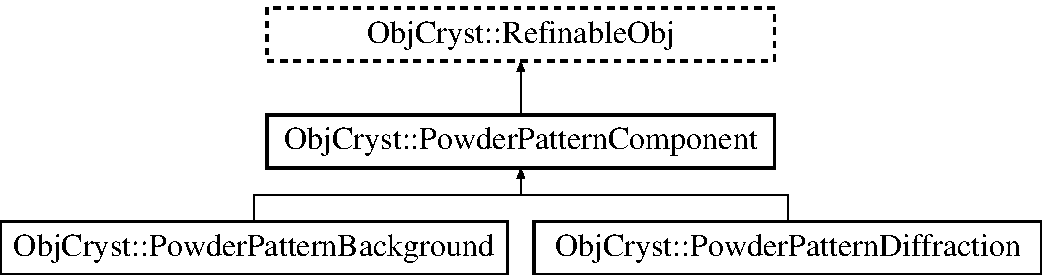
\includegraphics[height=3.000000cm]{a00072}
\end{center}
\end{figure}
\subsubsection*{Classes}
\begin{DoxyCompactItemize}
\item 
struct {\bf Refl\+Profile}
\begin{DoxyCompactList}\small\item\em Profile of a single reflection. \end{DoxyCompactList}\end{DoxyCompactItemize}
\subsubsection*{Public Member Functions}
\begin{DoxyCompactItemize}
\item 
{\bfseries Powder\+Pattern\+Diffraction} (const {\bf Powder\+Pattern\+Diffraction} \&)\label{a00072_a66a5dbb3c4a169bea2fd738b8e2ad4b1}

\item 
virtual {\bf Powder\+Pattern\+Diffraction} $\ast$ {\bf Create\+Copy} () const \label{a00072_ab288a964d5259f2b239c49eb3efdd5bb}

\begin{DoxyCompactList}\small\item\em So-\/called virtual copy constructor. \end{DoxyCompactList}\item 
virtual const string \& {\bf Get\+Class\+Name} () const 
\begin{DoxyCompactList}\small\item\em Name for this class (\char`\"{}\+Refinable\+Obj\char`\"{}, \char`\"{}\+Crystal\char`\"{},...). \end{DoxyCompactList}\item 
virtual void {\bf Set\+Parent\+Powder\+Pattern} ({\bf Powder\+Pattern} \&)
\begin{DoxyCompactList}\small\item\em Set the \doxyref{Powder\+Pattern}{p.}{a00068} object which uses this component. \end{DoxyCompactList}\item 
virtual const Cryst\+Vector\+\_\+\+R\+E\+A\+L \& {\bf Get\+Powder\+Pattern\+Calc} () const 
\begin{DoxyCompactList}\small\item\em Get the calculated powder pattern for this component. \end{DoxyCompactList}\item 
virtual pair$<$ const \\*
Cryst\+Vector\+\_\+\+R\+E\+A\+L $\ast$, const \\*
{\bf Refinable\+Obj\+Clock} $\ast$ $>$ {\bf Get\+Powder\+Pattern\+Integrated\+Calc} () const 
\begin{DoxyCompactList}\small\item\em Get the integrated values of the powder pattern. \end{DoxyCompactList}\item 
void {\bf Set\+Reflection\+Profile\+Par} (const {\bf Reflection\+Profile\+Type} prof, const R\+E\+A\+L fwhm\+Caglioti\+W, const R\+E\+A\+L fwhm\+Caglioti\+U=0, const R\+E\+A\+L fwhm\+Caglioti\+V=0, const R\+E\+A\+L eta0=0.\+5, const R\+E\+A\+L eta1=0.)
\begin{DoxyCompactList}\small\item\em Set reflection profile parameters. \end{DoxyCompactList}\item 
void {\bf Set\+Profile} ({\bf Reflection\+Profile} $\ast$prof)
\begin{DoxyCompactList}\small\item\em Assign a new profile. \end{DoxyCompactList}\item 
const {\bf Reflection\+Profile} \& {\bf Get\+Profile} () const \label{a00072_a36737a2dbb8be2af46f5c314171b419a}

\begin{DoxyCompactList}\small\item\em Get reflection profile. \end{DoxyCompactList}\item 
{\bf Reflection\+Profile} \& {\bf Get\+Profile} ()\label{a00072_a8f82b16e1d676f468475317afaddfdd8}

\begin{DoxyCompactList}\small\item\em Get reflection profile. \end{DoxyCompactList}\item 
virtual void {\bfseries Gen\+H\+K\+L\+Full\+Space} ()\label{a00072_a8d40f85ebf29e8f57c369ec2111650a4}

\item 
virtual void {\bf X\+M\+L\+Output} (ostream \&os, int indent=0) const 
\begin{DoxyCompactList}\small\item\em Output to stream in well-\/formed X\+M\+L. \end{DoxyCompactList}\item 
virtual void {\bf X\+M\+L\+Input} (istream \&is, const {\bf X\+M\+L\+Cryst\+Tag} \&tag)
\begin{DoxyCompactList}\small\item\em Input From stream. \end{DoxyCompactList}\item 
virtual void {\bf Get\+Gene\+Group} (const {\bf Refinable\+Obj} \&obj, Cryst\+Vector\+\_\+uint \&group\+Index, unsigned int \&first\+Group) const 
\begin{DoxyCompactList}\small\item\em Get the gene group assigned to each parameter. \end{DoxyCompactList}\item 
virtual void {\bf Begin\+Optimization} (const bool allow\+Approximations=false, const bool enable\+Restraints=false)
\begin{DoxyCompactList}\small\item\em This should be called by any optimization class at the begining of an optimization. \end{DoxyCompactList}\item 
virtual void {\bf End\+Optimization} ()
\begin{DoxyCompactList}\small\item\em This should be called by any optimization class at the end of an optimization. \end{DoxyCompactList}\item 
virtual void {\bf Set\+Approximation\+Flag} (const bool allow)
\begin{DoxyCompactList}\small\item\em Enable or disable numerical approximations. \end{DoxyCompactList}\item 
virtual const {\bf Radiation} \& {\bf Get\+Radiation} () const \label{a00072_a56744e8d8a61966b2acdc7c4ad9d4e85}

\begin{DoxyCompactList}\small\item\em Get the radiation object for this data. \end{DoxyCompactList}\item 
virtual const Cryst\+Vector\+\_\+\+R\+E\+A\+L \& {\bf Get\+Powder\+Pattern\+Calc\+Variance} () const 
\begin{DoxyCompactList}\small\item\em Get the variance associated to each point of the calculated powder pattern, for this component. \end{DoxyCompactList}\item 
virtual pair$<$ const \\*
Cryst\+Vector\+\_\+\+R\+E\+A\+L $\ast$, const \\*
{\bf Refinable\+Obj\+Clock} $\ast$ $>$ {\bf Get\+Powder\+Pattern\+Integrated\+Calc\+Variance} () const 
\begin{DoxyCompactList}\small\item\em Get the variance associated to each point of the calculated powder pattern, for this component (integrated version). \end{DoxyCompactList}\item 
virtual bool {\bf Has\+Powder\+Pattern\+Calc\+Variance} () const \label{a00072_ad0c57e0e2664e498e887d29698875cf0}

\begin{DoxyCompactList}\small\item\em Does this component have a variance associated with each calculated point ? i.\+e., do we use maximum likelihood to take into account incomplete models ? \end{DoxyCompactList}\item 
virtual void {\bf Set\+Crystal} ({\bf Crystal} \&crystal)
\begin{DoxyCompactList}\small\item\em Set the crystal for this experiment. \end{DoxyCompactList}\item 
void {\bf Set\+Extraction\+Mode} (const bool extract=true, const bool init=false)
\begin{DoxyCompactList}\small\item\em Prepare intensity extraction (Le Bail or Pawley) \end{DoxyCompactList}\item 
bool {\bf Get\+Extraction\+Mode} () const \label{a00072_add445d5800c4728a43c3c8a8bbea085d}

\begin{DoxyCompactList}\small\item\em Return true if in extraction mode, i.\+e. using extracted intensities instead of computed structure factors. \end{DoxyCompactList}\item 
void {\bf Extract\+Le\+Bail} (unsigned int nbcycle=1)
\begin{DoxyCompactList}\small\item\em Extract intensities using Le Bail method. \end{DoxyCompactList}\item 
virtual long {\bf Get\+Nb\+Refl\+Below\+Max\+Sin\+Theta\+Ov\+Lambda} () const 
\begin{DoxyCompactList}\small\item\em Recalc, and get the number of reflections which should be actually used, due to the maximuml sin(theta)/lambda value set. \end{DoxyCompactList}\end{DoxyCompactItemize}
\subsubsection*{Protected Member Functions}
\begin{DoxyCompactItemize}
\item 
virtual void {\bf Calc\+Powder\+Pattern} () const 
\begin{DoxyCompactList}\small\item\em Calc the powder pattern. \end{DoxyCompactList}\item 
virtual void {\bf Calc\+Powder\+Pattern\+Integrated} () const 
\begin{DoxyCompactList}\small\item\em Calc the integrated powder pattern. \end{DoxyCompactList}\item 
void {\bf Calc\+Powder\+Refl\+Profile} () const 
\item 
virtual void {\bf Calc\+Intensity\+Corr} () const 
\item 
virtual void {\bf Calc\+Ihkl} () const 
\item 
virtual void {\bf Prepare} ()
\item 
virtual void {\bfseries Init\+Options} ()\label{a00072_a734b53af6b0427541fa3ee852eb091f0}

\item 
virtual const Cryst\+Vector\+\_\+long \& {\bf Get\+Bragg\+Limits} () const 
\begin{DoxyCompactList}\small\item\em Get the pixel positions separating the integration intervals around reflections. \end{DoxyCompactList}\item 
virtual void {\bf Set\+Max\+Sin\+Theta\+Ov\+Lambda} (const R\+E\+A\+L max)
\begin{DoxyCompactList}\small\item\em Set the maximum value for sin(theta)/lambda. \end{DoxyCompactList}\item 
void {\bfseries Prepare\+Integrated\+Profile} () const \label{a00072_aacd4efcac37189dc542545563982f10e}

\end{DoxyCompactItemize}
\subsubsection*{Protected Attributes}
\begin{DoxyCompactItemize}
\item 
{\bf Refinable\+Obj\+Clock} {\bf m\+Clock\+Profile\+Par}\label{a00072_a509b94e52b44aed53752cdf92be7603c}

\begin{DoxyCompactList}\small\item\em Last time the reflection parameters were changed. \end{DoxyCompactList}\item 
{\bf Refinable\+Obj\+Clock} {\bf m\+Clock\+Lorentz\+Polar\+Slit\+Corr\+Par}\label{a00072_a1381bf49f3c4900f0e280f8bcbff172f}

\begin{DoxyCompactList}\small\item\em Last time the. \end{DoxyCompactList}\item 
{\bf Refinable\+Obj\+Clock} {\bf m\+Clock\+Intensity\+Corr}\label{a00072_ad963323e1ffbdadc9c7bd1cdbf9539dc}

\begin{DoxyCompactList}\small\item\em Last time the Lorentz-\/\+Polar-\/\+Slit correction was computed. \end{DoxyCompactList}\item 
{\bf Refinable\+Obj\+Clock} {\bf m\+Clock\+Profile\+Calc}\label{a00072_a39aa20a66d5c032083f96b96fe3f10d3}

\begin{DoxyCompactList}\small\item\em Last time the reflection profiles were computed. \end{DoxyCompactList}\item 
{\bf Refinable\+Obj\+Clock} {\bf m\+Clock\+Ihkl\+Calc}\label{a00072_a4b583c1ab76b3b39b891050f85e7d1f5}

\begin{DoxyCompactList}\small\item\em Last time intensities were computed. \end{DoxyCompactList}\item 
{\bf Reflection\+Profile} $\ast$ {\bf mp\+Reflection\+Profile}\label{a00072_ac7f248f736457fe513193865d2e154ad}

\begin{DoxyCompactList}\small\item\em Profile. \end{DoxyCompactList}\item 
Cryst\+Vector\+\_\+\+R\+E\+A\+L {\bf m\+Intensity\+Corr}
\begin{DoxyCompactList}\small\item\em Calculated corrections for all reflections. \end{DoxyCompactList}\item 
{\bf Lorentz\+Corr} {\bf m\+Corr\+Lorentz}\label{a00072_a7f83c3a22d2784ae9394ddd64e695088}

\begin{DoxyCompactList}\small\item\em Lorentz correction. \end{DoxyCompactList}\item 
{\bf Polarization\+Corr} {\bf m\+Corr\+Polar}\label{a00072_a38474f1c77cbc2b08c2d4354f8f439d1}

\begin{DoxyCompactList}\small\item\em Polarization correction. \end{DoxyCompactList}\item 
{\bf Powder\+Slit\+Aperture\+Corr} {\bf m\+Corr\+Slit\+Aperture}\label{a00072_ab2147524769083aaf24c8518ae4c6aab}

\begin{DoxyCompactList}\small\item\em Slit aperture correction. \end{DoxyCompactList}\item 
{\bf Texture\+March\+Dollase} {\bf m\+Corr\+Texture\+March\+Dollase}\label{a00072_aa2b7ce1dd0f5b396d9cbf86dcbe96b30}

\begin{DoxyCompactList}\small\item\em Preferred orientation (texture) correction following the March-\/\+Dollase model. \end{DoxyCompactList}\item 
{\bf T\+O\+F\+Corr} {\bf m\+Corr\+T\+O\+F}\label{a00072_a6a4defa4d63105fb531871c7460ac9b9}

\begin{DoxyCompactList}\small\item\em Time-\/\+Of-\/\+Flight intensity correction. \end{DoxyCompactList}\item 
Cryst\+Vector\+\_\+\+R\+E\+A\+L {\bf m\+Ihkl\+Calc}\label{a00072_aa312a4468b704f0bad83f5d06d4f470e}

\begin{DoxyCompactList}\small\item\em Computed intensities for all reflections. \end{DoxyCompactList}\item 
Cryst\+Vector\+\_\+\+R\+E\+A\+L {\bf m\+Ihkl\+Calc\+Variance}\label{a00072_ac74d96cb164d11c48fa24acb73b28008}

\begin{DoxyCompactList}\small\item\em Variance on computed intensities for all reflections. \end{DoxyCompactList}\item 
vector$<$ {\bf Refl\+Profile} $>$ {\bf mv\+Refl\+Profile}\label{a00072_aaff1e7365e403358c95ffb916b5914e8}

\begin{DoxyCompactList}\small\item\em Reflection profiles for A\+L\+L reflections during the last powder pattern generation. \end{DoxyCompactList}\item 
vector$<$ pair$<$ unsigned long, \\*
Cryst\+Vector\+\_\+\+R\+E\+A\+L $>$ $>$ {\bf m\+Integrated\+Profile\+Factor}
\begin{DoxyCompactList}\small\item\em For each reflection, store the integrated value of the normalized profile over all integration intervals. \end{DoxyCompactList}\item 
{\bf Refinable\+Obj\+Clock} {\bf m\+Clock\+Integrated\+Profile\+Factor}\label{a00072_a4abbf16a758485daab6392a875678abf}

\begin{DoxyCompactList}\small\item\em Last time the integrated values of normalized profiles was calculated. \end{DoxyCompactList}\item 
bool {\bfseries m\+Extraction\+Mode}\label{a00072_a3f0954b0ecb5786f8ca52ebb811c2ac0}

\item 
{\bf Diffraction\+Data\+Single\+Crystal} $\ast$ {\bf mp\+Le\+Bail\+Data}\label{a00072_ae03f55a0f790918e2ba366943f95b60d}

\begin{DoxyCompactList}\small\item\em Single crystal data extracted from the powder pattern. \end{DoxyCompactList}\item 
R\+E\+A\+L {\bf m\+Refl\+Prof\+Fact}\label{a00072_aaa33b091a2f27f60a1b43dac3c31e668}

\begin{DoxyCompactList}\small\item\em Range in which reflection profiles are calcualted is enlarged by this factor. \end{DoxyCompactList}\item 
R\+E\+A\+L {\bf m\+Refl\+Prof\+Min\+Rel\+Intensity}\label{a00072_aba6dba2fcbe1ecee0d230380fb4bc851}

\begin{DoxyCompactList}\small\item\em Minimum relative intensity for reflection profile calculation. \end{DoxyCompactList}\end{DoxyCompactItemize}


\subsubsection{Detailed Description}
Class to compute the contribution to a powder pattern from a crystalline phase. 

\subsubsection{Member Function Documentation}
\index{Obj\+Cryst\+::\+Powder\+Pattern\+Diffraction@{Obj\+Cryst\+::\+Powder\+Pattern\+Diffraction}!Begin\+Optimization@{Begin\+Optimization}}
\index{Begin\+Optimization@{Begin\+Optimization}!Obj\+Cryst\+::\+Powder\+Pattern\+Diffraction@{Obj\+Cryst\+::\+Powder\+Pattern\+Diffraction}}
\paragraph[{Begin\+Optimization}]{\setlength{\rightskip}{0pt plus 5cm}virtual void Obj\+Cryst\+::\+Powder\+Pattern\+Diffraction\+::\+Begin\+Optimization (
\begin{DoxyParamCaption}
\item[{const bool}]{allow\+Approximations = {\ttfamily false}, }
\item[{const bool}]{enable\+Restraints = {\ttfamily false}}
\end{DoxyParamCaption}
)\hspace{0.3cm}{\ttfamily [virtual]}}\label{a00072_a44d10a7c3404153fe4513c8944629c45}


This should be called by any optimization class at the begining of an optimization. 

This will also check that everything is ready, eg call the \doxyref{Refinable\+Obj\+::\+Prepare()}{p.}{a00077_a48d11671e7f8699f7bc24077585c5e0f} function. This also affects all sub-\/objects. \begin{DoxyNote}{Note}
this may be called several time for some objects which are used by several other objects, or for nested optimizations (e.\+g. least-\/squares optimizations inside a global one).

\doxyref{End\+Optimization()}{p.}{a00072_a11f7690878a07983de3abb839b087798} must be called at the end of the optimization, the same number of time \doxyref{Begin\+Optimization()}{p.}{a00072_a44d10a7c3404153fe4513c8944629c45} was called !
\end{DoxyNote}

\begin{DoxyParams}{Parameters}
{\em allow\+Approximations} & if true, then the object can use faster but less precise functions during the optimization. This is useful for global optimization not using derivatives. \\
\hline
{\em enable\+Restraints} & xrefitem deprecated 28. \\
\hline
\end{DoxyParams}


Reimplemented from {\bf Obj\+Cryst\+::\+Scattering\+Data} \doxyref{}{p.}{a00095_a6b0f18996edafa21a03bf9550dcf8981}.

\index{Obj\+Cryst\+::\+Powder\+Pattern\+Diffraction@{Obj\+Cryst\+::\+Powder\+Pattern\+Diffraction}!Calc\+Ihkl@{Calc\+Ihkl}}
\index{Calc\+Ihkl@{Calc\+Ihkl}!Obj\+Cryst\+::\+Powder\+Pattern\+Diffraction@{Obj\+Cryst\+::\+Powder\+Pattern\+Diffraction}}
\paragraph[{Calc\+Ihkl}]{\setlength{\rightskip}{0pt plus 5cm}virtual void Obj\+Cryst\+::\+Powder\+Pattern\+Diffraction\+::\+Calc\+Ihkl (
\begin{DoxyParamCaption}
{}
\end{DoxyParamCaption}
) const\hspace{0.3cm}{\ttfamily [protected]}, {\ttfamily [virtual]}}\label{a00072_a56dce436cf171bd33e8adc50d3c40fb8}
Compute the intensity for all reflections (taking into account corrections, but not the multiplicity) \index{Obj\+Cryst\+::\+Powder\+Pattern\+Diffraction@{Obj\+Cryst\+::\+Powder\+Pattern\+Diffraction}!Calc\+Intensity\+Corr@{Calc\+Intensity\+Corr}}
\index{Calc\+Intensity\+Corr@{Calc\+Intensity\+Corr}!Obj\+Cryst\+::\+Powder\+Pattern\+Diffraction@{Obj\+Cryst\+::\+Powder\+Pattern\+Diffraction}}
\paragraph[{Calc\+Intensity\+Corr}]{\setlength{\rightskip}{0pt plus 5cm}virtual void Obj\+Cryst\+::\+Powder\+Pattern\+Diffraction\+::\+Calc\+Intensity\+Corr (
\begin{DoxyParamCaption}
{}
\end{DoxyParamCaption}
) const\hspace{0.3cm}{\ttfamily [protected]}, {\ttfamily [virtual]}}\label{a00072_a4053e0b8996de211ba196310fa3feee9}
Calc Lorentz-\/\+Polarisation-\/\+A\+Perture correction \index{Obj\+Cryst\+::\+Powder\+Pattern\+Diffraction@{Obj\+Cryst\+::\+Powder\+Pattern\+Diffraction}!Calc\+Powder\+Pattern@{Calc\+Powder\+Pattern}}
\index{Calc\+Powder\+Pattern@{Calc\+Powder\+Pattern}!Obj\+Cryst\+::\+Powder\+Pattern\+Diffraction@{Obj\+Cryst\+::\+Powder\+Pattern\+Diffraction}}
\paragraph[{Calc\+Powder\+Pattern}]{\setlength{\rightskip}{0pt plus 5cm}virtual void Obj\+Cryst\+::\+Powder\+Pattern\+Diffraction\+::\+Calc\+Powder\+Pattern (
\begin{DoxyParamCaption}
{}
\end{DoxyParamCaption}
) const\hspace{0.3cm}{\ttfamily [protected]}, {\ttfamily [virtual]}}\label{a00072_a1f37b1e47c8bef989931fac08cf18849}


Calc the powder pattern. 

As always, recomputation is only done if necessary (ie if a parameter has changed since the last computation) 

Implements {\bf Obj\+Cryst\+::\+Powder\+Pattern\+Component} \doxyref{}{p.}{a00071_a8417ecb93009a9b7b9fccf074a9438d9}.

\index{Obj\+Cryst\+::\+Powder\+Pattern\+Diffraction@{Obj\+Cryst\+::\+Powder\+Pattern\+Diffraction}!Calc\+Powder\+Pattern\+Integrated@{Calc\+Powder\+Pattern\+Integrated}}
\index{Calc\+Powder\+Pattern\+Integrated@{Calc\+Powder\+Pattern\+Integrated}!Obj\+Cryst\+::\+Powder\+Pattern\+Diffraction@{Obj\+Cryst\+::\+Powder\+Pattern\+Diffraction}}
\paragraph[{Calc\+Powder\+Pattern\+Integrated}]{\setlength{\rightskip}{0pt plus 5cm}virtual void Obj\+Cryst\+::\+Powder\+Pattern\+Diffraction\+::\+Calc\+Powder\+Pattern\+Integrated (
\begin{DoxyParamCaption}
{}
\end{DoxyParamCaption}
) const\hspace{0.3cm}{\ttfamily [protected]}, {\ttfamily [virtual]}}\label{a00072_ae9e715bb230da8a3683adfee296288ad}


Calc the integrated powder pattern. 

This should be optimized so that the full powder pattern is not explicitely computed. 

Implements {\bf Obj\+Cryst\+::\+Powder\+Pattern\+Component} \doxyref{}{p.}{a00071_a24c4fb58e500cd669f3298475a31f72f}.

\index{Obj\+Cryst\+::\+Powder\+Pattern\+Diffraction@{Obj\+Cryst\+::\+Powder\+Pattern\+Diffraction}!Calc\+Powder\+Refl\+Profile@{Calc\+Powder\+Refl\+Profile}}
\index{Calc\+Powder\+Refl\+Profile@{Calc\+Powder\+Refl\+Profile}!Obj\+Cryst\+::\+Powder\+Pattern\+Diffraction@{Obj\+Cryst\+::\+Powder\+Pattern\+Diffraction}}
\paragraph[{Calc\+Powder\+Refl\+Profile}]{\setlength{\rightskip}{0pt plus 5cm}void Obj\+Cryst\+::\+Powder\+Pattern\+Diffraction\+::\+Calc\+Powder\+Refl\+Profile (
\begin{DoxyParamCaption}
{}
\end{DoxyParamCaption}
) const\hspace{0.3cm}{\ttfamily [protected]}}\label{a00072_add8efa98500f554fd35bf672a999d949}
Calc reflection profiles for A\+L\+L reflections (powder diffraction) \index{Obj\+Cryst\+::\+Powder\+Pattern\+Diffraction@{Obj\+Cryst\+::\+Powder\+Pattern\+Diffraction}!End\+Optimization@{End\+Optimization}}
\index{End\+Optimization@{End\+Optimization}!Obj\+Cryst\+::\+Powder\+Pattern\+Diffraction@{Obj\+Cryst\+::\+Powder\+Pattern\+Diffraction}}
\paragraph[{End\+Optimization}]{\setlength{\rightskip}{0pt plus 5cm}virtual void Obj\+Cryst\+::\+Powder\+Pattern\+Diffraction\+::\+End\+Optimization (
\begin{DoxyParamCaption}
{}
\end{DoxyParamCaption}
)\hspace{0.3cm}{\ttfamily [virtual]}}\label{a00072_a11f7690878a07983de3abb839b087798}


This should be called by any optimization class at the end of an optimization. 

This also affects all sub-\/objects. \begin{DoxyNote}{Note}
this may be called several time for some objects which are used by several other objects. 
\end{DoxyNote}


Reimplemented from {\bf Obj\+Cryst\+::\+Scattering\+Data} \doxyref{}{p.}{a00095_a782e0caf5c6f2941ca64d17293b1e8b4}.

\index{Obj\+Cryst\+::\+Powder\+Pattern\+Diffraction@{Obj\+Cryst\+::\+Powder\+Pattern\+Diffraction}!Extract\+Le\+Bail@{Extract\+Le\+Bail}}
\index{Extract\+Le\+Bail@{Extract\+Le\+Bail}!Obj\+Cryst\+::\+Powder\+Pattern\+Diffraction@{Obj\+Cryst\+::\+Powder\+Pattern\+Diffraction}}
\paragraph[{Extract\+Le\+Bail}]{\setlength{\rightskip}{0pt plus 5cm}void Obj\+Cryst\+::\+Powder\+Pattern\+Diffraction\+::\+Extract\+Le\+Bail (
\begin{DoxyParamCaption}
\item[{unsigned int}]{nbcycle = {\ttfamily 1}}
\end{DoxyParamCaption}
)}\label{a00072_aa86150b55c39275e7d076afb2b43513d}


Extract intensities using Le Bail method. 


\begin{DoxyParams}{Parameters}
{\em nbcycle} & number of cycles \\
\hline
\end{DoxyParams}
\index{Obj\+Cryst\+::\+Powder\+Pattern\+Diffraction@{Obj\+Cryst\+::\+Powder\+Pattern\+Diffraction}!Get\+Bragg\+Limits@{Get\+Bragg\+Limits}}
\index{Get\+Bragg\+Limits@{Get\+Bragg\+Limits}!Obj\+Cryst\+::\+Powder\+Pattern\+Diffraction@{Obj\+Cryst\+::\+Powder\+Pattern\+Diffraction}}
\paragraph[{Get\+Bragg\+Limits}]{\setlength{\rightskip}{0pt plus 5cm}virtual const Cryst\+Vector\+\_\+long\& Obj\+Cryst\+::\+Powder\+Pattern\+Diffraction\+::\+Get\+Bragg\+Limits (
\begin{DoxyParamCaption}
{}
\end{DoxyParamCaption}
) const\hspace{0.3cm}{\ttfamily [protected]}, {\ttfamily [virtual]}}\label{a00072_ab9e21f6f16d77e96e4b5bed47db82dca}


Get the pixel positions separating the integration intervals around reflections. 

\begin{DoxyReturn}{Returns}
\+: an array with the pixel positions, empty if this component has no peaks. The positions should be in increasing order, but could go beyond the pattern limits. 
\end{DoxyReturn}


Implements {\bf Obj\+Cryst\+::\+Powder\+Pattern\+Component} \doxyref{}{p.}{a00071_a727488f859528b0a9b5da47973804e01}.

\index{Obj\+Cryst\+::\+Powder\+Pattern\+Diffraction@{Obj\+Cryst\+::\+Powder\+Pattern\+Diffraction}!Get\+Class\+Name@{Get\+Class\+Name}}
\index{Get\+Class\+Name@{Get\+Class\+Name}!Obj\+Cryst\+::\+Powder\+Pattern\+Diffraction@{Obj\+Cryst\+::\+Powder\+Pattern\+Diffraction}}
\paragraph[{Get\+Class\+Name}]{\setlength{\rightskip}{0pt plus 5cm}virtual const string\& Obj\+Cryst\+::\+Powder\+Pattern\+Diffraction\+::\+Get\+Class\+Name (
\begin{DoxyParamCaption}
{}
\end{DoxyParamCaption}
) const\hspace{0.3cm}{\ttfamily [virtual]}}\label{a00072_a74b02e35219c6bc18521e66719778881}


Name for this class (\char`\"{}\+Refinable\+Obj\char`\"{}, \char`\"{}\+Crystal\char`\"{},...). 

This is only useful to distinguish different classes when picking up objects from the \doxyref{Refinable\+Obj}{p.}{a00077} Global Registry 

Reimplemented from {\bf Obj\+Cryst\+::\+Powder\+Pattern\+Component} \doxyref{}{p.}{a00071_a5e797476d8d76ef797e1e8b51db9e8fb}.

\index{Obj\+Cryst\+::\+Powder\+Pattern\+Diffraction@{Obj\+Cryst\+::\+Powder\+Pattern\+Diffraction}!Get\+Gene\+Group@{Get\+Gene\+Group}}
\index{Get\+Gene\+Group@{Get\+Gene\+Group}!Obj\+Cryst\+::\+Powder\+Pattern\+Diffraction@{Obj\+Cryst\+::\+Powder\+Pattern\+Diffraction}}
\paragraph[{Get\+Gene\+Group}]{\setlength{\rightskip}{0pt plus 5cm}virtual void Obj\+Cryst\+::\+Powder\+Pattern\+Diffraction\+::\+Get\+Gene\+Group (
\begin{DoxyParamCaption}
\item[{const {\bf Refinable\+Obj} \&}]{obj, }
\item[{Cryst\+Vector\+\_\+uint \&}]{group\+Index, }
\item[{unsigned int \&}]{first\+Group}
\end{DoxyParamCaption}
) const\hspace{0.3cm}{\ttfamily [virtual]}}\label{a00072_a7c6a94f74a6010abdb9ba4d5a8653d3f}


Get the gene group assigned to each parameter. 

Each parameter (a {\itshape gene} in terms of genetic algorithms) can be assigned to a gene group. Thus when mating two configurations, genes will be exchanged by groups. By default (in the base Refinabe\+Obj class), each parameter is alone in its group. Derived classes can group genes for a better s$\ast$$\ast$ life.

The number identifying a gene group only has a meaning in a given object. It can also change on subsequent calls, and thus is not unique.


\begin{DoxyParams}{Parameters}
{\em obj} & the , supplied by an algorithm class (\doxyref{Optimization\+Obj}{p.}{a00061},..), which contains a list of parameters, some of which (but possibly all or none) are parameters belonging to this object. \\
\hline
{\em group\+Index} & a vector of unsigned integers, one for each parameter in the input object, giving an unsigned integer value as gene group index. At the beginning this vector should contain only zeros (no group assigned). \\
\hline
{\em first\+Group} & this is the number of groups which have already been assigned, plus one. The gene groups returned by this object will start from this value, and increment {\bfseries first\+Group} for each gene group used, so that different \doxyref{Refinable\+Obj}{p.}{a00077} cannot share a gene group. \\
\hline
\end{DoxyParams}
\begin{DoxyNote}{Note}
this function is not optimized, and should only be called at the beginning of a refinement. 
\end{DoxyNote}


Reimplemented from {\bf Obj\+Cryst\+::\+Refinable\+Obj} \doxyref{}{p.}{a00077_ad59c8ad2b0d7ee59fa3f399a54f05e54}.

\index{Obj\+Cryst\+::\+Powder\+Pattern\+Diffraction@{Obj\+Cryst\+::\+Powder\+Pattern\+Diffraction}!Get\+Nb\+Refl\+Below\+Max\+Sin\+Theta\+Ov\+Lambda@{Get\+Nb\+Refl\+Below\+Max\+Sin\+Theta\+Ov\+Lambda}}
\index{Get\+Nb\+Refl\+Below\+Max\+Sin\+Theta\+Ov\+Lambda@{Get\+Nb\+Refl\+Below\+Max\+Sin\+Theta\+Ov\+Lambda}!Obj\+Cryst\+::\+Powder\+Pattern\+Diffraction@{Obj\+Cryst\+::\+Powder\+Pattern\+Diffraction}}
\paragraph[{Get\+Nb\+Refl\+Below\+Max\+Sin\+Theta\+Ov\+Lambda}]{\setlength{\rightskip}{0pt plus 5cm}virtual long Obj\+Cryst\+::\+Powder\+Pattern\+Diffraction\+::\+Get\+Nb\+Refl\+Below\+Max\+Sin\+Theta\+Ov\+Lambda (
\begin{DoxyParamCaption}
{}
\end{DoxyParamCaption}
) const\hspace{0.3cm}{\ttfamily [virtual]}}\label{a00072_a2793f8d2df13e5a1e9a5efc527771b3a}


Recalc, and get the number of reflections which should be actually used, due to the maximuml sin(theta)/lambda value set. 



Reimplemented from {\bf Obj\+Cryst\+::\+Scattering\+Data} \doxyref{}{p.}{a00095_aac8034f8b0f6980c619e595ce6ba1d65}.

\index{Obj\+Cryst\+::\+Powder\+Pattern\+Diffraction@{Obj\+Cryst\+::\+Powder\+Pattern\+Diffraction}!Get\+Powder\+Pattern\+Calc@{Get\+Powder\+Pattern\+Calc}}
\index{Get\+Powder\+Pattern\+Calc@{Get\+Powder\+Pattern\+Calc}!Obj\+Cryst\+::\+Powder\+Pattern\+Diffraction@{Obj\+Cryst\+::\+Powder\+Pattern\+Diffraction}}
\paragraph[{Get\+Powder\+Pattern\+Calc}]{\setlength{\rightskip}{0pt plus 5cm}virtual const Cryst\+Vector\+\_\+\+R\+E\+A\+L\& Obj\+Cryst\+::\+Powder\+Pattern\+Diffraction\+::\+Get\+Powder\+Pattern\+Calc (
\begin{DoxyParamCaption}
{}
\end{DoxyParamCaption}
) const\hspace{0.3cm}{\ttfamily [virtual]}}\label{a00072_a8003dc9bbaf67b5d95e443c20166b742}


Get the calculated powder pattern for this component. 

Note that the pattern is {\itshape not} scaled. 

Implements {\bf Obj\+Cryst\+::\+Powder\+Pattern\+Component} \doxyref{}{p.}{a00071_a45258e9f9b44ff019bf53aa3dfb1a305}.

\index{Obj\+Cryst\+::\+Powder\+Pattern\+Diffraction@{Obj\+Cryst\+::\+Powder\+Pattern\+Diffraction}!Get\+Powder\+Pattern\+Calc\+Variance@{Get\+Powder\+Pattern\+Calc\+Variance}}
\index{Get\+Powder\+Pattern\+Calc\+Variance@{Get\+Powder\+Pattern\+Calc\+Variance}!Obj\+Cryst\+::\+Powder\+Pattern\+Diffraction@{Obj\+Cryst\+::\+Powder\+Pattern\+Diffraction}}
\paragraph[{Get\+Powder\+Pattern\+Calc\+Variance}]{\setlength{\rightskip}{0pt plus 5cm}virtual const Cryst\+Vector\+\_\+\+R\+E\+A\+L\& Obj\+Cryst\+::\+Powder\+Pattern\+Diffraction\+::\+Get\+Powder\+Pattern\+Calc\+Variance (
\begin{DoxyParamCaption}
{}
\end{DoxyParamCaption}
) const\hspace{0.3cm}{\ttfamily [virtual]}}\label{a00072_a664e1f47391720d06ffaa2b10b0aaf49}


Get the variance associated to each point of the calculated powder pattern, for this component. 

\begin{DoxyWarning}{Warning}
\+: this is experimental, with the aim of using Maximum Likelihood to improve structure determination. 
\end{DoxyWarning}


Implements {\bf Obj\+Cryst\+::\+Powder\+Pattern\+Component} \doxyref{}{p.}{a00071_ad67b39669fd0d336b01937ee81a59ddc}.

\index{Obj\+Cryst\+::\+Powder\+Pattern\+Diffraction@{Obj\+Cryst\+::\+Powder\+Pattern\+Diffraction}!Get\+Powder\+Pattern\+Integrated\+Calc@{Get\+Powder\+Pattern\+Integrated\+Calc}}
\index{Get\+Powder\+Pattern\+Integrated\+Calc@{Get\+Powder\+Pattern\+Integrated\+Calc}!Obj\+Cryst\+::\+Powder\+Pattern\+Diffraction@{Obj\+Cryst\+::\+Powder\+Pattern\+Diffraction}}
\paragraph[{Get\+Powder\+Pattern\+Integrated\+Calc}]{\setlength{\rightskip}{0pt plus 5cm}virtual pair$<$const Cryst\+Vector\+\_\+\+R\+E\+A\+L$\ast$,const {\bf Refinable\+Obj\+Clock}$\ast$$>$ Obj\+Cryst\+::\+Powder\+Pattern\+Diffraction\+::\+Get\+Powder\+Pattern\+Integrated\+Calc (
\begin{DoxyParamCaption}
{}
\end{DoxyParamCaption}
) const\hspace{0.3cm}{\ttfamily [virtual]}}\label{a00072_a2f2a745dcfa6cb7b7af4523b268827fe}


Get the integrated values of the powder pattern. 

\begin{DoxyNote}{Note}
\+: the integration intervals are those given by the parent \doxyref{Powder\+Pattern}{p.}{a00068}, so that all \doxyref{Powder\+Pattern\+Component}{p.}{a00071}'s intervals are taken into account
\end{DoxyNote}
This avoids explicitely calculating the full profile powder pattern. 

Implements {\bf Obj\+Cryst\+::\+Powder\+Pattern\+Component} \doxyref{}{p.}{a00071_ac54b7ae5a177492de681afc2cbed72eb}.

\index{Obj\+Cryst\+::\+Powder\+Pattern\+Diffraction@{Obj\+Cryst\+::\+Powder\+Pattern\+Diffraction}!Get\+Powder\+Pattern\+Integrated\+Calc\+Variance@{Get\+Powder\+Pattern\+Integrated\+Calc\+Variance}}
\index{Get\+Powder\+Pattern\+Integrated\+Calc\+Variance@{Get\+Powder\+Pattern\+Integrated\+Calc\+Variance}!Obj\+Cryst\+::\+Powder\+Pattern\+Diffraction@{Obj\+Cryst\+::\+Powder\+Pattern\+Diffraction}}
\paragraph[{Get\+Powder\+Pattern\+Integrated\+Calc\+Variance}]{\setlength{\rightskip}{0pt plus 5cm}virtual pair$<$const Cryst\+Vector\+\_\+\+R\+E\+A\+L$\ast$,const {\bf Refinable\+Obj\+Clock}$\ast$$>$ Obj\+Cryst\+::\+Powder\+Pattern\+Diffraction\+::\+Get\+Powder\+Pattern\+Integrated\+Calc\+Variance (
\begin{DoxyParamCaption}
{}
\end{DoxyParamCaption}
) const\hspace{0.3cm}{\ttfamily [virtual]}}\label{a00072_ae529ea1dab34388e88ba4a818ed48ca1}


Get the variance associated to each point of the calculated powder pattern, for this component (integrated version). 

\begin{DoxyWarning}{Warning}
\+: this is experimental, with the aim of using Maximum Likelihood to improve structure determination. 
\end{DoxyWarning}


Implements {\bf Obj\+Cryst\+::\+Powder\+Pattern\+Component} \doxyref{}{p.}{a00071_ae721bd290b50aa9503bac419616a21c6}.

\index{Obj\+Cryst\+::\+Powder\+Pattern\+Diffraction@{Obj\+Cryst\+::\+Powder\+Pattern\+Diffraction}!Prepare@{Prepare}}
\index{Prepare@{Prepare}!Obj\+Cryst\+::\+Powder\+Pattern\+Diffraction@{Obj\+Cryst\+::\+Powder\+Pattern\+Diffraction}}
\paragraph[{Prepare}]{\setlength{\rightskip}{0pt plus 5cm}virtual void Obj\+Cryst\+::\+Powder\+Pattern\+Diffraction\+::\+Prepare (
\begin{DoxyParamCaption}
{}
\end{DoxyParamCaption}
)\hspace{0.3cm}{\ttfamily [protected]}, {\ttfamily [virtual]}}\label{a00072_ae19852383674ae3ab673748a30a8432a}
This will be called by the parent \doxyref{Powder\+Pattern}{p.}{a00068} object, before calculating the first powder pattern. Or maybe it should be called automatically by the object itself... 

Implements {\bf Obj\+Cryst\+::\+Powder\+Pattern\+Component} \doxyref{}{p.}{a00071_a6a99877f0f9dec09fd5f596a7ddeb6f6}.

\index{Obj\+Cryst\+::\+Powder\+Pattern\+Diffraction@{Obj\+Cryst\+::\+Powder\+Pattern\+Diffraction}!Set\+Approximation\+Flag@{Set\+Approximation\+Flag}}
\index{Set\+Approximation\+Flag@{Set\+Approximation\+Flag}!Obj\+Cryst\+::\+Powder\+Pattern\+Diffraction@{Obj\+Cryst\+::\+Powder\+Pattern\+Diffraction}}
\paragraph[{Set\+Approximation\+Flag}]{\setlength{\rightskip}{0pt plus 5cm}virtual void Obj\+Cryst\+::\+Powder\+Pattern\+Diffraction\+::\+Set\+Approximation\+Flag (
\begin{DoxyParamCaption}
\item[{const bool}]{allow}
\end{DoxyParamCaption}
)\hspace{0.3cm}{\ttfamily [virtual]}}\label{a00072_a0e7b4a6f4b3a7b783ebed15230a1c45f}


Enable or disable numerical approximations. 

This can be used for global optimization to get faster calculations. Depending on the type of object, this may do something or not (it does not do anything in a base \doxyref{Refinable\+Obj}{p.}{a00077}, except calling this function for all sub-\/objects).

\begin{DoxyNote}{Note}
Currently there is no m\+Approximation\+Flag in the base class, but maybe there should...
\end{DoxyNote}
Also see\+: 

Reimplemented from {\bf Obj\+Cryst\+::\+Scattering\+Data} \doxyref{}{p.}{a00095_a109ed8c2e8dc676e77aa80feafa91071}.

\index{Obj\+Cryst\+::\+Powder\+Pattern\+Diffraction@{Obj\+Cryst\+::\+Powder\+Pattern\+Diffraction}!Set\+Crystal@{Set\+Crystal}}
\index{Set\+Crystal@{Set\+Crystal}!Obj\+Cryst\+::\+Powder\+Pattern\+Diffraction@{Obj\+Cryst\+::\+Powder\+Pattern\+Diffraction}}
\paragraph[{Set\+Crystal}]{\setlength{\rightskip}{0pt plus 5cm}virtual void Obj\+Cryst\+::\+Powder\+Pattern\+Diffraction\+::\+Set\+Crystal (
\begin{DoxyParamCaption}
\item[{{\bf Crystal} \&}]{crystal}
\end{DoxyParamCaption}
)\hspace{0.3cm}{\ttfamily [virtual]}}\label{a00072_a855f114ce585410a354b56a6ea336eaf}


Set the crystal for this experiment. 



Reimplemented from {\bf Obj\+Cryst\+::\+Scattering\+Data} \doxyref{}{p.}{a00095_a75ea37efc16db856fff9b8832b524284}.

\index{Obj\+Cryst\+::\+Powder\+Pattern\+Diffraction@{Obj\+Cryst\+::\+Powder\+Pattern\+Diffraction}!Set\+Extraction\+Mode@{Set\+Extraction\+Mode}}
\index{Set\+Extraction\+Mode@{Set\+Extraction\+Mode}!Obj\+Cryst\+::\+Powder\+Pattern\+Diffraction@{Obj\+Cryst\+::\+Powder\+Pattern\+Diffraction}}
\paragraph[{Set\+Extraction\+Mode}]{\setlength{\rightskip}{0pt plus 5cm}void Obj\+Cryst\+::\+Powder\+Pattern\+Diffraction\+::\+Set\+Extraction\+Mode (
\begin{DoxyParamCaption}
\item[{const bool}]{extract = {\ttfamily true}, }
\item[{const bool}]{init = {\ttfamily false}}
\end{DoxyParamCaption}
)}\label{a00072_a02f1293bc57c472a85741a328521d95f}


Prepare intensity extraction (Le Bail or Pawley) 


\begin{DoxyParams}{Parameters}
{\em extract} & if true, begin extraction mode, else enable structure factor calculations \\
\hline
{\em init} & if true and extract=true, intensities are set to 100 \\
\hline
\end{DoxyParams}
\index{Obj\+Cryst\+::\+Powder\+Pattern\+Diffraction@{Obj\+Cryst\+::\+Powder\+Pattern\+Diffraction}!Set\+Max\+Sin\+Theta\+Ov\+Lambda@{Set\+Max\+Sin\+Theta\+Ov\+Lambda}}
\index{Set\+Max\+Sin\+Theta\+Ov\+Lambda@{Set\+Max\+Sin\+Theta\+Ov\+Lambda}!Obj\+Cryst\+::\+Powder\+Pattern\+Diffraction@{Obj\+Cryst\+::\+Powder\+Pattern\+Diffraction}}
\paragraph[{Set\+Max\+Sin\+Theta\+Ov\+Lambda}]{\setlength{\rightskip}{0pt plus 5cm}virtual void Obj\+Cryst\+::\+Powder\+Pattern\+Diffraction\+::\+Set\+Max\+Sin\+Theta\+Ov\+Lambda (
\begin{DoxyParamCaption}
\item[{const R\+E\+A\+L}]{max}
\end{DoxyParamCaption}
)\hspace{0.3cm}{\ttfamily [protected]}, {\ttfamily [virtual]}}\label{a00072_a699af7ea523fca128032384b548ceef1}


Set the maximum value for sin(theta)/lambda. 

All data above still exist but are ignored for all calculations. 

Implements {\bf Obj\+Cryst\+::\+Powder\+Pattern\+Component} \doxyref{}{p.}{a00071_a4731b5a64ee9aab6779e2ef323242fe5}.

\index{Obj\+Cryst\+::\+Powder\+Pattern\+Diffraction@{Obj\+Cryst\+::\+Powder\+Pattern\+Diffraction}!Set\+Parent\+Powder\+Pattern@{Set\+Parent\+Powder\+Pattern}}
\index{Set\+Parent\+Powder\+Pattern@{Set\+Parent\+Powder\+Pattern}!Obj\+Cryst\+::\+Powder\+Pattern\+Diffraction@{Obj\+Cryst\+::\+Powder\+Pattern\+Diffraction}}
\paragraph[{Set\+Parent\+Powder\+Pattern}]{\setlength{\rightskip}{0pt plus 5cm}virtual void Obj\+Cryst\+::\+Powder\+Pattern\+Diffraction\+::\+Set\+Parent\+Powder\+Pattern (
\begin{DoxyParamCaption}
\item[{{\bf Powder\+Pattern} \&}]{}
\end{DoxyParamCaption}
)\hspace{0.3cm}{\ttfamily [virtual]}}\label{a00072_ab67953ad7f27c37334a6b557c2da1d73}


Set the \doxyref{Powder\+Pattern}{p.}{a00068} object which uses this component. 

This sets all necessary pattern parameters (2theta/tof range, wavelength, radiation type...) accordingly. 

Implements {\bf Obj\+Cryst\+::\+Powder\+Pattern\+Component} \doxyref{}{p.}{a00071_a6b3dc911118c280dbbdcb7fb97acf980}.

\index{Obj\+Cryst\+::\+Powder\+Pattern\+Diffraction@{Obj\+Cryst\+::\+Powder\+Pattern\+Diffraction}!Set\+Profile@{Set\+Profile}}
\index{Set\+Profile@{Set\+Profile}!Obj\+Cryst\+::\+Powder\+Pattern\+Diffraction@{Obj\+Cryst\+::\+Powder\+Pattern\+Diffraction}}
\paragraph[{Set\+Profile}]{\setlength{\rightskip}{0pt plus 5cm}void Obj\+Cryst\+::\+Powder\+Pattern\+Diffraction\+::\+Set\+Profile (
\begin{DoxyParamCaption}
\item[{{\bf Reflection\+Profile} $\ast$}]{prof}
\end{DoxyParamCaption}
)}\label{a00072_abf4e4d356004068fc2ae2faaaf40c336}


Assign a new profile. 

\index{Obj\+Cryst\+::\+Powder\+Pattern\+Diffraction@{Obj\+Cryst\+::\+Powder\+Pattern\+Diffraction}!Set\+Reflection\+Profile\+Par@{Set\+Reflection\+Profile\+Par}}
\index{Set\+Reflection\+Profile\+Par@{Set\+Reflection\+Profile\+Par}!Obj\+Cryst\+::\+Powder\+Pattern\+Diffraction@{Obj\+Cryst\+::\+Powder\+Pattern\+Diffraction}}
\paragraph[{Set\+Reflection\+Profile\+Par}]{\setlength{\rightskip}{0pt plus 5cm}void Obj\+Cryst\+::\+Powder\+Pattern\+Diffraction\+::\+Set\+Reflection\+Profile\+Par (
\begin{DoxyParamCaption}
\item[{const {\bf Reflection\+Profile\+Type}}]{prof, }
\item[{const R\+E\+A\+L}]{fwhm\+Caglioti\+W, }
\item[{const R\+E\+A\+L}]{fwhm\+Caglioti\+U = {\ttfamily 0}, }
\item[{const R\+E\+A\+L}]{fwhm\+Caglioti\+V = {\ttfamily 0}, }
\item[{const R\+E\+A\+L}]{eta0 = {\ttfamily 0.5}, }
\item[{const R\+E\+A\+L}]{eta1 = {\ttfamily 0.}}
\end{DoxyParamCaption}
)}\label{a00072_a7e75337a21cc715aefb78ed70d30dba7}


Set reflection profile parameters. 

\+:T\+O\+D\+O\+: assymmetric profiles 
\begin{DoxyParams}{Parameters}
{\em fwhm\+Caglioti\+W,fwhm\+Caglioti\+U,fwhm\+Caglioti\+V} & \+: these are the U,V and W parameters in the Caglioti's law \+: $ fwhm^2= U \tan^2(\theta) + V \tan(\theta) +W $ if only W is given, the width is constant \\
\hline
{\em eta0,eta1} & these are the mixing parameters in the case of a pseudo-\/\+Voigt function. \\
\hline
\end{DoxyParams}
\index{Obj\+Cryst\+::\+Powder\+Pattern\+Diffraction@{Obj\+Cryst\+::\+Powder\+Pattern\+Diffraction}!X\+M\+L\+Input@{X\+M\+L\+Input}}
\index{X\+M\+L\+Input@{X\+M\+L\+Input}!Obj\+Cryst\+::\+Powder\+Pattern\+Diffraction@{Obj\+Cryst\+::\+Powder\+Pattern\+Diffraction}}
\paragraph[{X\+M\+L\+Input}]{\setlength{\rightskip}{0pt plus 5cm}virtual void Obj\+Cryst\+::\+Powder\+Pattern\+Diffraction\+::\+X\+M\+L\+Input (
\begin{DoxyParamCaption}
\item[{istream \&}]{is, }
\item[{const {\bf X\+M\+L\+Cryst\+Tag} \&}]{tag}
\end{DoxyParamCaption}
)\hspace{0.3cm}{\ttfamily [virtual]}}\label{a00072_af350a4a95ddac5f15812bf35015f83fb}


Input From stream. 

\begin{DoxyRefDesc}{Todo}
\item[{\bf Todo}]Add an bool X\+M\+L\+Input\+Tag(is,tag) function to recognize all the tags from the stream. So that each inherited class can use the X\+M\+L\+Input\+Tag function from its parent (ie take advantage of inheritance). The children class would first try to interpret the tag, then if unsuccessful would pass it to its parent (thus allowing overloading), etc... \end{DoxyRefDesc}


Reimplemented from {\bf Obj\+Cryst\+::\+Refinable\+Obj} \doxyref{}{p.}{a00077_ac13a4045c3f187879443c8615c38d623}.

\index{Obj\+Cryst\+::\+Powder\+Pattern\+Diffraction@{Obj\+Cryst\+::\+Powder\+Pattern\+Diffraction}!X\+M\+L\+Output@{X\+M\+L\+Output}}
\index{X\+M\+L\+Output@{X\+M\+L\+Output}!Obj\+Cryst\+::\+Powder\+Pattern\+Diffraction@{Obj\+Cryst\+::\+Powder\+Pattern\+Diffraction}}
\paragraph[{X\+M\+L\+Output}]{\setlength{\rightskip}{0pt plus 5cm}virtual void Obj\+Cryst\+::\+Powder\+Pattern\+Diffraction\+::\+X\+M\+L\+Output (
\begin{DoxyParamCaption}
\item[{ostream \&}]{os, }
\item[{int}]{indent = {\ttfamily 0}}
\end{DoxyParamCaption}
) const\hspace{0.3cm}{\ttfamily [virtual]}}\label{a00072_af4a2a4dbdbc9eb85274835a4b3d10be9}


Output to stream in well-\/formed X\+M\+L. 

\begin{DoxyRefDesc}{Todo}
\item[{\bf Todo}]Use inheritance.. as for X\+M\+L\+Input\+Tag()... \end{DoxyRefDesc}


Reimplemented from {\bf Obj\+Cryst\+::\+Refinable\+Obj} \doxyref{}{p.}{a00077_a7b9b6ed0f8dcf753d398c35e073de973}.



\subsubsection{Member Data Documentation}
\index{Obj\+Cryst\+::\+Powder\+Pattern\+Diffraction@{Obj\+Cryst\+::\+Powder\+Pattern\+Diffraction}!m\+Integrated\+Profile\+Factor@{m\+Integrated\+Profile\+Factor}}
\index{m\+Integrated\+Profile\+Factor@{m\+Integrated\+Profile\+Factor}!Obj\+Cryst\+::\+Powder\+Pattern\+Diffraction@{Obj\+Cryst\+::\+Powder\+Pattern\+Diffraction}}
\paragraph[{m\+Integrated\+Profile\+Factor}]{\setlength{\rightskip}{0pt plus 5cm}vector$<$ pair$<$unsigned long, Cryst\+Vector\+\_\+\+R\+E\+A\+L$>$ $>$ Obj\+Cryst\+::\+Powder\+Pattern\+Diffraction\+::m\+Integrated\+Profile\+Factor\hspace{0.3cm}{\ttfamily [mutable]}, {\ttfamily [protected]}}\label{a00072_a551115d02944f3e0d360cc92f8084c99}


For each reflection, store the integrated value of the normalized profile over all integration intervals. 

The first field is the first integration interval to which the reflection contributes, and the second field is a vector with all the integrated values for the intervals, listed in ascending 2theta(tof) order. \index{Obj\+Cryst\+::\+Powder\+Pattern\+Diffraction@{Obj\+Cryst\+::\+Powder\+Pattern\+Diffraction}!m\+Intensity\+Corr@{m\+Intensity\+Corr}}
\index{m\+Intensity\+Corr@{m\+Intensity\+Corr}!Obj\+Cryst\+::\+Powder\+Pattern\+Diffraction@{Obj\+Cryst\+::\+Powder\+Pattern\+Diffraction}}
\paragraph[{m\+Intensity\+Corr}]{\setlength{\rightskip}{0pt plus 5cm}Cryst\+Vector\+\_\+\+R\+E\+A\+L Obj\+Cryst\+::\+Powder\+Pattern\+Diffraction\+::m\+Intensity\+Corr\hspace{0.3cm}{\ttfamily [mutable]}, {\ttfamily [protected]}}\label{a00072_addc10ae4a02801eb441e38b4beae2e9a}


Calculated corrections for all reflections. 

Calc F$^\wedge$2 must be multiplied by this factor to yield intensities.

Thus we have \+: $ I_{hkl} = L \times P \times SlitAp \times F_{hkl}^2 $

with $ L = \frac{1}{\sin(2\theta)} $ (Lorentz factor). $ P = \frac{1}{1+A}\left(1+A\cos^2(2\theta)\right) $ (Polarization factor), with $ A = \frac{1-f}{1+f} $, where f is the polarization rate of the incident beam in the plane which (i) includes the incident beam, and (ii) is perpendicular to the diffracting plane. For an X-\/\+Ray Tube without monochromator, A=1, and if there is a monochromator \+: $ A = \cos^2(2\theta_{mono}) $ The factor $ SlitAp = \frac{1}{\sin(\theta)} $ takes into account the fraction of the diffracted cone which falls in the detector slit.

If there is prefereed orientation, this also holds the associated correction.

\begin{DoxyRefDesc}{Todo}
\item[{\bf Todo}]\+: store all corrections in a registry, so that other corrections can more easily be added (? Maybe not that useful, especially since these correction do not need to be displayed to the user ?). \end{DoxyRefDesc}


The documentation for this class was generated from the following file\+:\begin{DoxyCompactItemize}
\item 
Powder\+Pattern.\+h\end{DoxyCompactItemize}

\subsection{Obj\+Cryst\+:\+:Powder\+Slit\+Aperture\+Corr Class Reference}
\label{a00073}\index{Obj\+Cryst\+::\+Powder\+Slit\+Aperture\+Corr@{Obj\+Cryst\+::\+Powder\+Slit\+Aperture\+Corr}}


Slit aperture correction (for powder)  


Inheritance diagram for Obj\+Cryst\+:\+:Powder\+Slit\+Aperture\+Corr\+:\begin{figure}[H]
\begin{center}
\leavevmode
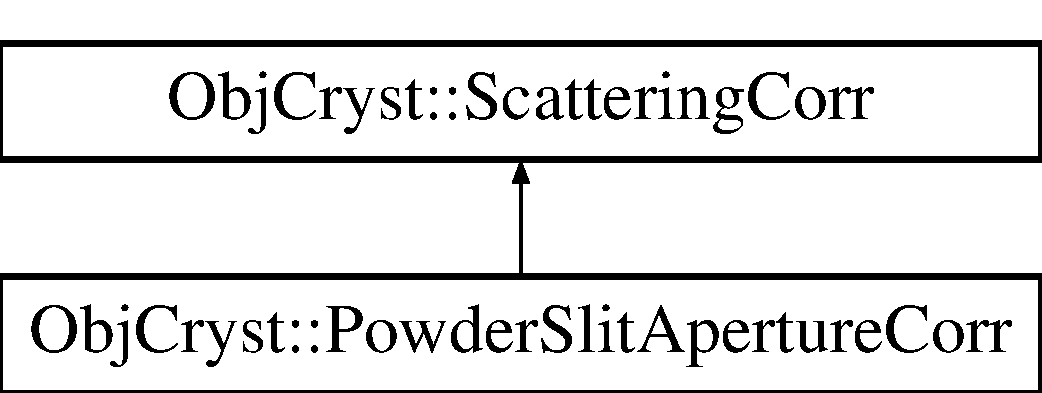
\includegraphics[height=2.000000cm]{a00073}
\end{center}
\end{figure}
\subsubsection*{Public Member Functions}
\begin{DoxyCompactItemize}
\item 
{\bfseries Powder\+Slit\+Aperture\+Corr} (const {\bf Scattering\+Data} \&data)\label{a00073_a8c7814fd23c9e2fe96a904ea41137caf}

\item 
virtual const string \& {\bf Get\+Name} () const \label{a00073_a395cb337777d1c3fdd283f03c9a06e27}

\begin{DoxyCompactList}\small\item\em Get the name of this object. \end{DoxyCompactList}\item 
virtual const string \& {\bf Get\+Class\+Name} () const \label{a00073_a36c1dd123d3f951ba140796f47a68fbb}

\begin{DoxyCompactList}\small\item\em Get the name of the class. \end{DoxyCompactList}\end{DoxyCompactItemize}
\subsubsection*{Protected Member Functions}
\begin{DoxyCompactItemize}
\item 
virtual void {\bf Calc\+Corr} () const \label{a00073_ae7b2fecebc30de79ccc54f5237ec67f7}

\begin{DoxyCompactList}\small\item\em Do the computation of corrected intensities. \end{DoxyCompactList}\end{DoxyCompactItemize}
\subsubsection*{Additional Inherited Members}


\subsubsection{Detailed Description}
Slit aperture correction (for powder) 

This correction takes into account the fact that diffraction rings (cones) have a portion of the ring proportionnal to $ SlitAp = \frac{1}{\sin(\theta)} $ which falls into the detector (due to slits in the direction perpendicular to the incident beam/ detector plane). 

The documentation for this class was generated from the following file\+:\begin{DoxyCompactItemize}
\item 
Scattering\+Corr.\+h\end{DoxyCompactItemize}

\subsection{\-Obj\-Cryst\-:\-:\-Reflection\-Profile \-Class \-Reference}
\label{a00074}\index{\-Obj\-Cryst\-::\-Reflection\-Profile@{\-Obj\-Cryst\-::\-Reflection\-Profile}}


\-Abstract base class for reflection profiles.  


\-Inheritance diagram for \-Obj\-Cryst\-:\-:\-Reflection\-Profile\-:\begin{figure}[H]
\begin{center}
\leavevmode
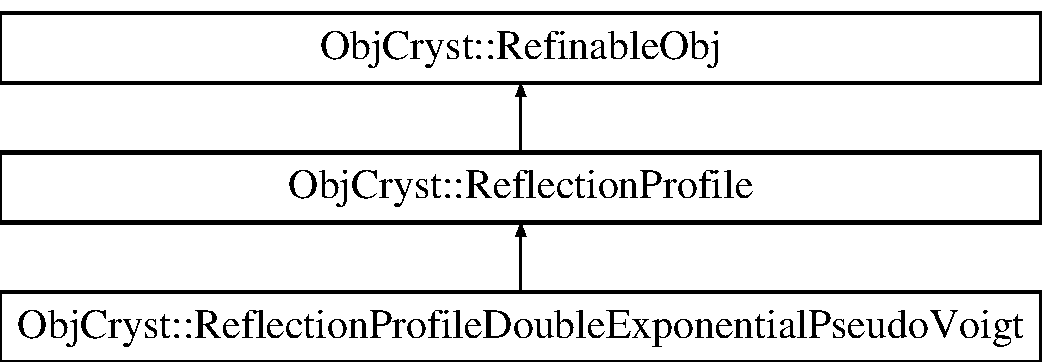
\includegraphics[height=2.434783cm]{a00074}
\end{center}
\end{figure}
\subsubsection*{\-Public \-Member \-Functions}
\begin{DoxyCompactItemize}
\item 
{\bfseries \-Reflection\-Profile} (const {\bf \-Reflection\-Profile} \&old)\label{a00074_a4647aa58d8e98429b10c54499b9b050e}

\item 
virtual {\bf \-Reflection\-Profile} $\ast$ {\bfseries \-Create\-Copy} () const =0\label{a00074_a620f88c536f3c13881262efd155cc504}

\item 
virtual \-Cryst\-Vector\-\_\-\-R\-E\-A\-L {\bf \-Get\-Profile} (const \-Cryst\-Vector\-\_\-\-R\-E\-A\-L \&x, const \-R\-E\-A\-L xcenter, const \-R\-E\-A\-L h, const \-R\-E\-A\-L k, const \-R\-E\-A\-L l)=0
\begin{DoxyCompactList}\small\item\em \-Get the reflection profile. \end{DoxyCompactList}\item 
virtual \-R\-E\-A\-L {\bf \-Get\-Full\-Profile\-Width} (const \-R\-E\-A\-L relative\-Intensity, const \-R\-E\-A\-L xcenter, const \-R\-E\-A\-L h, const \-R\-E\-A\-L k, const \-R\-E\-A\-L l)=0
\begin{DoxyCompactList}\small\item\em \-Get the (approximate) full profile width at a given percentage of the profile maximum (e.\-g. \end{DoxyCompactList}\item 
virtual bool {\bf \-Is\-Anisotropic} () const \label{a00074_ad1c2083adc170bc0d84b44f17b79d008}

\begin{DoxyCompactList}\small\item\em \-Is the profile anisotropic ? \end{DoxyCompactList}\item 
virtual void {\bf \-X\-M\-L\-Output} (ostream \&os, int indent=0) const =0
\begin{DoxyCompactList}\small\item\em \-Output to stream in well-\/formed \-X\-M\-L. \end{DoxyCompactList}\item 
virtual void {\bf \-X\-M\-L\-Input} (istream \&is, const {\bf \-X\-M\-L\-Cryst\-Tag} \&tag)=0
\begin{DoxyCompactList}\small\item\em \-Input \-From stream. \end{DoxyCompactList}\end{DoxyCompactItemize}


\subsubsection{\-Detailed \-Description}
\-Abstract base class for reflection profiles. 

\subsubsection{\-Member \-Function \-Documentation}
\index{\-Obj\-Cryst\-::\-Reflection\-Profile@{\-Obj\-Cryst\-::\-Reflection\-Profile}!\-Get\-Full\-Profile\-Width@{\-Get\-Full\-Profile\-Width}}
\index{\-Get\-Full\-Profile\-Width@{\-Get\-Full\-Profile\-Width}!ObjCryst::ReflectionProfile@{\-Obj\-Cryst\-::\-Reflection\-Profile}}
\paragraph[{\-Get\-Full\-Profile\-Width}]{\setlength{\rightskip}{0pt plus 5cm}virtual \-R\-E\-A\-L {\bf \-Obj\-Cryst\-::\-Reflection\-Profile\-::\-Get\-Full\-Profile\-Width} (
\begin{DoxyParamCaption}
\item[{const \-R\-E\-A\-L}]{relative\-Intensity, }
\item[{const \-R\-E\-A\-L}]{xcenter, }
\item[{const \-R\-E\-A\-L}]{h, }
\item[{const \-R\-E\-A\-L}]{k, }
\item[{const \-R\-E\-A\-L}]{l}
\end{DoxyParamCaption}
)\hspace{0.3cm}{\ttfamily  [pure virtual]}}\label{a00074_ac6d2a69e63c3efd06f30ab134062bbc0}


\-Get the (approximate) full profile width at a given percentage of the profile maximum (e.\-g. 

\-F\-W\-H\-M=\-Get\-Full\-Profile\-Width(0.\-5)). 

\-Implemented in {\bf \-Obj\-Cryst\-::\-Reflection\-Profile\-Double\-Exponential\-Pseudo\-Voigt} \doxyref{}{p.}{a00075_ac1c2c1f3673f4558eca2c7bee8c3fdea}, and {\bf \-Obj\-Cryst\-::\-Reflection\-Profile\-Pseudo\-Voigt} \doxyref{}{p.}{a00076_abacd734b6ff73b4fc5e6c4a5cba62eb6}.

\index{\-Obj\-Cryst\-::\-Reflection\-Profile@{\-Obj\-Cryst\-::\-Reflection\-Profile}!\-Get\-Profile@{\-Get\-Profile}}
\index{\-Get\-Profile@{\-Get\-Profile}!ObjCryst::ReflectionProfile@{\-Obj\-Cryst\-::\-Reflection\-Profile}}
\paragraph[{\-Get\-Profile}]{\setlength{\rightskip}{0pt plus 5cm}virtual \-Cryst\-Vector\-\_\-\-R\-E\-A\-L {\bf \-Obj\-Cryst\-::\-Reflection\-Profile\-::\-Get\-Profile} (
\begin{DoxyParamCaption}
\item[{const \-Cryst\-Vector\-\_\-\-R\-E\-A\-L \&}]{x, }
\item[{const \-R\-E\-A\-L}]{xcenter, }
\item[{const \-R\-E\-A\-L}]{h, }
\item[{const \-R\-E\-A\-L}]{k, }
\item[{const \-R\-E\-A\-L}]{l}
\end{DoxyParamCaption}
)\hspace{0.3cm}{\ttfamily  [pure virtual]}}\label{a00074_a93a92759349fa242b1c3ed6bb7b24979}


\-Get the reflection profile. 


\begin{DoxyParams}{\-Parameters}
{\em x,\-:} & the vector of x coordinates (i.\-e. either 2theta or time-\/of-\/flight) \\
\hline
{\em xcenter,\-:} & coordinate (2theta, tof) of the center of the peak \\
\hline
{\em h,k,l,\-:} & reflection \-Miller indices \\
\hline
\end{DoxyParams}
\begin{DoxyNote}{\-Note}
\-: derived classes who need either d\-\_\-hkl or the orthonormal coordinates of the scattering vector should be passed a \doxyref{\-Obj\-Cryst\-::\-Unit\-Cell}{p.}{a00110} object in the constructor so that they can use \doxyref{\-Obj\-Cryst\-::\-Unit\-Cell\-::\-Miller\-To\-Orthonormal\-Coords()}{p.}{a00110_af6efcbafcd761c6f8f4953190e7024d0} 
\end{DoxyNote}


\-Implemented in {\bf \-Obj\-Cryst\-::\-Reflection\-Profile\-Double\-Exponential\-Pseudo\-Voigt} \doxyref{}{p.}{a00075_ab7c71a3e6156a66f4210fea3086db8d6}, and {\bf \-Obj\-Cryst\-::\-Reflection\-Profile\-Pseudo\-Voigt} \doxyref{}{p.}{a00076_a14ba03c411e8b3d2d4f5af46e6504658}.

\index{\-Obj\-Cryst\-::\-Reflection\-Profile@{\-Obj\-Cryst\-::\-Reflection\-Profile}!\-X\-M\-L\-Input@{\-X\-M\-L\-Input}}
\index{\-X\-M\-L\-Input@{\-X\-M\-L\-Input}!ObjCryst::ReflectionProfile@{\-Obj\-Cryst\-::\-Reflection\-Profile}}
\paragraph[{\-X\-M\-L\-Input}]{\setlength{\rightskip}{0pt plus 5cm}virtual void {\bf \-Obj\-Cryst\-::\-Reflection\-Profile\-::\-X\-M\-L\-Input} (
\begin{DoxyParamCaption}
\item[{istream \&}]{is, }
\item[{const {\bf \-X\-M\-L\-Cryst\-Tag} \&}]{tag}
\end{DoxyParamCaption}
)\hspace{0.3cm}{\ttfamily  [pure virtual]}}\label{a00074_a7ad38593ddb4601632beb0a6bcae50f3}


\-Input \-From stream. 

\begin{DoxyRefDesc}{\-Todo}
\item[{\bf \-Todo}]\-Add an bool \-X\-M\-L\-Input\-Tag(is,tag) function to recognize all the tags from the stream. \-So that each inherited class can use the \-X\-M\-L\-Input\-Tag function from its parent (ie take advantage of inheritance). \-The children class would first try to interpret the tag, then if unsuccessful would pass it to its parent (thus allowing overloading), etc... \end{DoxyRefDesc}


\-Reimplemented from {\bf \-Obj\-Cryst\-::\-Refinable\-Obj} \doxyref{}{p.}{a00071_ac13a4045c3f187879443c8615c38d623}.



\-Implemented in {\bf \-Obj\-Cryst\-::\-Reflection\-Profile\-Double\-Exponential\-Pseudo\-Voigt} \doxyref{}{p.}{a00075_a4965f2a8994475187423a7afd6943031}, and {\bf \-Obj\-Cryst\-::\-Reflection\-Profile\-Pseudo\-Voigt} \doxyref{}{p.}{a00076_a8c63700610f511503eae297c8161f311}.

\index{\-Obj\-Cryst\-::\-Reflection\-Profile@{\-Obj\-Cryst\-::\-Reflection\-Profile}!\-X\-M\-L\-Output@{\-X\-M\-L\-Output}}
\index{\-X\-M\-L\-Output@{\-X\-M\-L\-Output}!ObjCryst::ReflectionProfile@{\-Obj\-Cryst\-::\-Reflection\-Profile}}
\paragraph[{\-X\-M\-L\-Output}]{\setlength{\rightskip}{0pt plus 5cm}virtual void {\bf \-Obj\-Cryst\-::\-Reflection\-Profile\-::\-X\-M\-L\-Output} (
\begin{DoxyParamCaption}
\item[{ostream \&}]{os, }
\item[{int}]{indent = {\ttfamily 0}}
\end{DoxyParamCaption}
) const\hspace{0.3cm}{\ttfamily  [pure virtual]}}\label{a00074_a60e429bb999a8b39f09ef14cdaf5ad0c}


\-Output to stream in well-\/formed \-X\-M\-L. 

\begin{DoxyRefDesc}{\-Todo}
\item[{\bf \-Todo}]\-Use inheritance.. as for \-X\-M\-L\-Input\-Tag()... \end{DoxyRefDesc}


\-Reimplemented from {\bf \-Obj\-Cryst\-::\-Refinable\-Obj} \doxyref{}{p.}{a00071_a7b9b6ed0f8dcf753d398c35e073de973}.



\-Implemented in {\bf \-Obj\-Cryst\-::\-Reflection\-Profile\-Double\-Exponential\-Pseudo\-Voigt} \doxyref{}{p.}{a00075_a6ec9818370703767da5362960c5b310a}, and {\bf \-Obj\-Cryst\-::\-Reflection\-Profile\-Pseudo\-Voigt} \doxyref{}{p.}{a00076_ac0438d3a1827accbdf2375e7355f18e5}.



\-The documentation for this class was generated from the following file\-:\begin{DoxyCompactItemize}
\item 
\-Reflection\-Profile.\-h\end{DoxyCompactItemize}

\subsection{Obj\-Cryst\-:\-:Radiation Class Reference}
\label{a00075}\index{Obj\-Cryst\-::\-Radiation@{Obj\-Cryst\-::\-Radiation}}


Class to define the radiation (type, monochromaticity, wavelength(s)) of an experiment.  


Inheritance diagram for Obj\-Cryst\-:\-:Radiation\-:\begin{figure}[H]
\begin{center}
\leavevmode
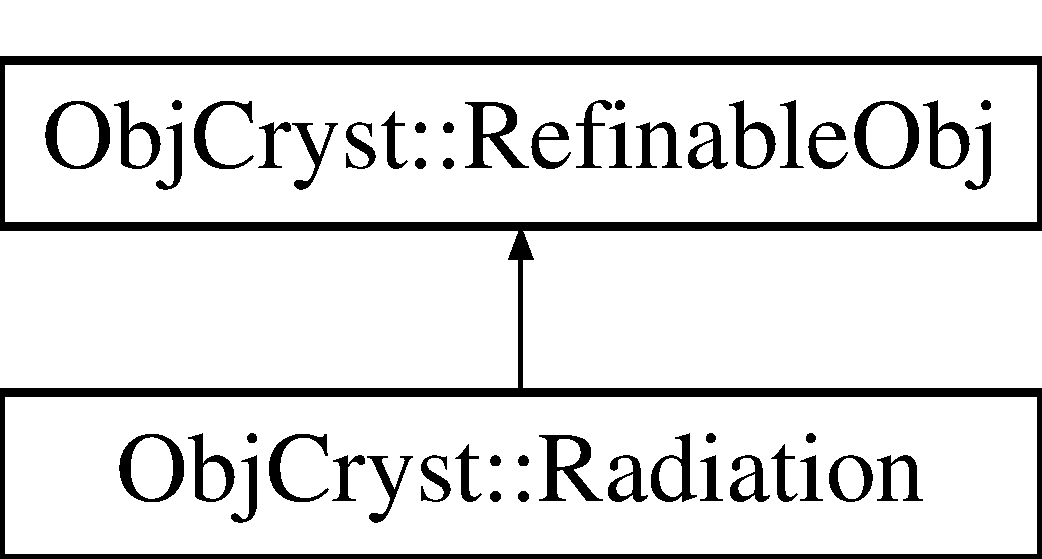
\includegraphics[height=2.000000cm]{a00075}
\end{center}
\end{figure}
\subsubsection*{Public Member Functions}
\begin{DoxyCompactItemize}
\item 
{\bf Radiation} ()\label{a00075_abd533ac660e70618339636f18d1347f4}

\begin{DoxyCompactList}\small\item\em Default constructor. \end{DoxyCompactList}\item 
{\bf Radiation} (const {\bf Radiation\-Type} rad, const R\-E\-A\-L wavelength)
\begin{DoxyCompactList}\small\item\em \textbackslash{} brief Constructor \end{DoxyCompactList}\item 
{\bf Radiation} (const string \&X\-Ray\-Tube\-Element\-Name, const R\-E\-A\-L alpha2\-Alpha2ratio=0.\-5)
\begin{DoxyCompactList}\small\item\em \textbackslash{} brief Constructor for X-\/\-Ray tube radiation \end{DoxyCompactList}\item 
{\bf Radiation} (const {\bf Radiation} \&)\label{a00075_ab08e37b8dd00149612aa656f1641a76f}

\begin{DoxyCompactList}\small\item\em Copy constructor. \end{DoxyCompactList}\item 
virtual const string \& {\bf Get\-Class\-Name} () const 
\begin{DoxyCompactList}\small\item\em Name for this class (\char`\"{}\-Refinable\-Obj\char`\"{}, \char`\"{}\-Crystal\char`\"{},...). \end{DoxyCompactList}\item 
void {\bfseries operator=} (const {\bf Radiation} \&)\label{a00075_aaa4a0199b2d383fb69c0de13c62a024c}

\item 
{\bf Radiation\-Type} {\bf Get\-Radiation\-Type} () const \label{a00075_a3c4e81e8db0ea43c42278948c56ba46f}

\begin{DoxyCompactList}\small\item\em Get the radiation type (X-\/\-Rays, Neutron) \end{DoxyCompactList}\item 
void {\bf Set\-Radiation\-Type} (const {\bf Radiation\-Type})\label{a00075_a8fd969b9f546fc48f5bfd7b38ff9c995}

\begin{DoxyCompactList}\small\item\em Set the radiation type (X-\/\-Rays, Neutron) \end{DoxyCompactList}\item 
void {\bf Set\-Wavelength\-Type} (const {\bf Wavelength\-Type} \&type)\label{a00075_adc4fac12bb11e01e515365e5d7a46ddc}

\begin{DoxyCompactList}\small\item\em Set the Wavelength type (monochromatic, Alpha1+\-Alpha2, Time Of Flight...) \end{DoxyCompactList}\item 
{\bf Wavelength\-Type} {\bf Get\-Wavelength\-Type} () const \label{a00075_ab1c21d1a6344287a8c4271c2b7a12c79}

\begin{DoxyCompactList}\small\item\em Get the Wavelength type (monochromatic, Alpha1+\-Alpha2, Time Of Flight...) \end{DoxyCompactList}\item 
const Cryst\-Vector\-\_\-\-R\-E\-A\-L \& {\bf Get\-Wavelength} () const 
\begin{DoxyCompactList}\small\item\em Get the wavelength(s) in Angstroems. \end{DoxyCompactList}\item 
void {\bf Set\-Wavelength} (const R\-E\-A\-L)\label{a00075_ac40cb0879be00b232a6c3e78c069823d}

\begin{DoxyCompactList}\small\item\em Set the (monochromatic) wavelength of the beam. \end{DoxyCompactList}\item 
void {\bf Set\-Wavelength} (const string \&X\-Ray\-Tube\-Element\-Name, const R\-E\-A\-L alpha2\-Alpha2ratio=0.\-5)
\begin{DoxyCompactList}\small\item\em \textbackslash{} brief Set X-\/\-Ray tube radiation. \end{DoxyCompactList}\item 
R\-E\-A\-L {\bf Get\-X\-Ray\-Tube\-Delta\-Lambda} () const \label{a00075_aaacaaa8568c368b0f39d4ee8cea95576}

\begin{DoxyCompactList}\small\item\em Get the wavelength difference for Alpha1 and Alpha2. \end{DoxyCompactList}\item 
R\-E\-A\-L {\bf Get\-X\-Ray\-Tube\-Alpha2\-Alpha1\-Ratio} () const \label{a00075_aa2016f3b8df9727cc59d74f137f2c626}

\begin{DoxyCompactList}\small\item\em Get the Kalpha2/\-Kalpha1 ratio. \end{DoxyCompactList}\item 
const {\bf Refinable\-Obj\-Clock} \& {\bf Get\-Clock\-Wavelength} () const \label{a00075_a049b5bed7c75b14ad1e5e84ff945b7fa}

\begin{DoxyCompactList}\small\item\em Last time the wavelength has been changed. \end{DoxyCompactList}\item 
const {\bf Refinable\-Obj\-Clock} \& {\bf Get\-Clock\-Radiation} () const \label{a00075_ac3085d33817e372b906527d89d06fa8f}

\begin{DoxyCompactList}\small\item\em Last time the nature (X-\/\-Rays/\-Neutron, number of wavelengths)radiation has been changed. \end{DoxyCompactList}\item 
virtual void {\bf X\-M\-L\-Output} (ostream \&os, int indent=0) const 
\begin{DoxyCompactList}\small\item\em Output to stream in well-\/formed X\-M\-L. \end{DoxyCompactList}\item 
virtual void {\bf X\-M\-L\-Input} (istream \&is, const {\bf X\-M\-L\-Cryst\-Tag} \&tag)
\begin{DoxyCompactList}\small\item\em Input From stream. \end{DoxyCompactList}\item 
void {\bf Print} () const \label{a00075_a74fa173d33eb724be83a2ede6042dce3}

\begin{DoxyCompactList}\small\item\em Print to screen/console the charcteristics of the radiation. \end{DoxyCompactList}\item 
R\-E\-A\-L {\bfseries Get\-Linear\-Polar\-Rate} () const \label{a00075_a103b3216086ff11bfe3465e2d057fbda}

\item 
void {\bfseries Set\-Linear\-Polar\-Rate} (const R\-E\-A\-L f)\label{a00075_a9602288c888944773e93fa67f8542d95}

\end{DoxyCompactItemize}
\subsubsection*{Private Member Functions}
\begin{DoxyCompactItemize}
\item 
void {\bfseries Init\-Options} ()\label{a00075_a4663c4bfeb1bb617f77896179fb0a2d2}

\end{DoxyCompactItemize}
\subsubsection*{Private Attributes}
\begin{DoxyCompactItemize}
\item 
{\bf Ref\-Obj\-Opt} {\bf m\-Radiation\-Type}\label{a00075_a3b736f32b507d8e0f4ebd8b46e50659b}

\begin{DoxyCompactList}\small\item\em Neutron ? X-\/\-Ray ? (Electron\-: unimplemented) \end{DoxyCompactList}\item 
{\bf Ref\-Obj\-Opt} {\bf m\-Wavelength\-Type}\label{a00075_a9ef30865d93e28dbba31fee53c4c39aa}

\begin{DoxyCompactList}\small\item\em monochromatic ? Alpha1 \& Alpha2 ? Multi-\/\-Wavelength ? \end{DoxyCompactList}\item 
Cryst\-Vector\-\_\-\-R\-E\-A\-L {\bf m\-Wavelength}\label{a00075_a1c786f2e4a6035954fc76cb7cb7ad736}

\begin{DoxyCompactList}\small\item\em Wavelength of the Experiment, in Angstroems. \end{DoxyCompactList}\item 
string {\bf m\-X\-Ray\-Tube\-Name}
\begin{DoxyCompactList}\small\item\em Name of the X-\/\-Ray tube used, if relevant. \end{DoxyCompactList}\item 
R\-E\-A\-L {\bf m\-X\-Ray\-Tube\-Delta\-Lambda}\label{a00075_a66546a093f76ef3b9822be44e98ca17f}

\begin{DoxyCompactList}\small\item\em Absolute difference between alpha1 and alpha2, in angstroems. \end{DoxyCompactList}\item 
R\-E\-A\-L {\bf m\-X\-Ray\-Tube\-Alpha2\-Alpha1\-Ratio}\label{a00075_a72fd03ef0f28986f3ea66fd96d040688}

\begin{DoxyCompactList}\small\item\em Ratio alpha2/alpha1 (should be 0.\-5) \end{DoxyCompactList}\item 
{\bf Refinable\-Obj\-Clock} {\bfseries m\-Clock\-Wavelength}\label{a00075_af492e24a913e63781a53946feecb6ffc}

\item 
{\bf Refinable\-Obj\-Clock} {\bfseries m\-Clock\-Radiation}\label{a00075_a255532a6369c7265df67aabba103153f}

\item 
R\-E\-A\-L {\bf m\-Linear\-Polar\-Rate}\label{a00075_a0e8a10c625ae1bd2733e830c2ca7d606}

\begin{DoxyCompactList}\small\item\em Linear Polarization Rate (default\-:0, X-\/\-Ray tube unmonochromatized) \end{DoxyCompactList}\end{DoxyCompactItemize}
\subsubsection*{Additional Inherited Members}


\subsubsection{Detailed Description}
Class to define the radiation (type, monochromaticity, wavelength(s)) of an experiment. 

This can be developped for more complex experiments, hence the {\itshape vector} of wavelengths (so far it is not possible to use several wavelengths, though).

X-\/\-Rays and Neutrons are available. Electrons are not available yet in \doxyref{Scattering\-Data}{p.}{a00095} classes.

\begin{DoxyRefDesc}{Todo}
\item[{\bf Todo}]also add here information about the polarization of the beam. \end{DoxyRefDesc}


\subsubsection{Constructor \& Destructor Documentation}
\index{Obj\-Cryst\-::\-Radiation@{Obj\-Cryst\-::\-Radiation}!Radiation@{Radiation}}
\index{Radiation@{Radiation}!ObjCryst::Radiation@{Obj\-Cryst\-::\-Radiation}}
\paragraph[{Radiation}]{\setlength{\rightskip}{0pt plus 5cm}Obj\-Cryst\-::\-Radiation\-::\-Radiation (
\begin{DoxyParamCaption}
\item[{const {\bf Radiation\-Type}}]{rad, }
\item[{const R\-E\-A\-L}]{wavelength}
\end{DoxyParamCaption}
)}\label{a00075_ace67fea27bc640ac4820fc1ba73114d5}


\textbackslash{} brief Constructor 


\begin{DoxyParams}{Parameters}
{\em rad} & the Radiation\-Type used (X-\/\-Rays, neutrons) \\
\hline
{\em wavelength} & the wavelength (in Angstroems) of the monochromatic radiation. \\
\hline
\end{DoxyParams}
\index{Obj\-Cryst\-::\-Radiation@{Obj\-Cryst\-::\-Radiation}!Radiation@{Radiation}}
\index{Radiation@{Radiation}!ObjCryst::Radiation@{Obj\-Cryst\-::\-Radiation}}
\paragraph[{Radiation}]{\setlength{\rightskip}{0pt plus 5cm}Obj\-Cryst\-::\-Radiation\-::\-Radiation (
\begin{DoxyParamCaption}
\item[{const string \&}]{X\-Ray\-Tube\-Element\-Name, }
\item[{const R\-E\-A\-L}]{alpha2\-Alpha2ratio = {\ttfamily 0.5}}
\end{DoxyParamCaption}
)}\label{a00075_a0302f8a0f706db01d0ada609c2e427d4}


\textbackslash{} brief Constructor for X-\/\-Ray tube radiation 


\begin{DoxyParams}{Parameters}
{\em X\-Ray\-Tube\-Element\-Name} & \-: name of the anticathode element name. Known ones are Cr, Fe, Cu, Mo, Ag. \\
\hline
{\em alpha2\-Alpha2ratio} & Kalpha2/\-Kalpha1 ratio (0.\-5 by default)\\
\hline
\end{DoxyParams}
the average wavelength is calculated using the alpha2/alpha1 weight. All structure factors computation are made using the average wavelength, and for powder diffraction, profiles are output at the alpha1 and alpha2 ratio for the calculated pattern.

N\-O\-T\-E \-: if the name of the wavelength is generic (eg\char`\"{}\-Cu\char`\"{}), then the program considers that there are both Alpha1 and Alpha2, and thus automatically changes the Wavelength\-Type to W\-A\-V\-E\-L\-E\-N\-G\-T\-H\-\_\-\-A\-L\-P\-H\-A12. If instead either alpha1 or alpha2 (eg \char`\"{}\-Cu\-A1\char`\"{}) is asked for, the Wavelength\-Type is set to W\-A\-V\-E\-L\-E\-N\-G\-T\-H\-\_\-\-M\-O\-N\-O\-C\-H\-R\-O\-M\-A\-T\-I\-C. In both cases, the radiation type is set to X-\/\-Ray. 

\subsubsection{Member Function Documentation}
\index{Obj\-Cryst\-::\-Radiation@{Obj\-Cryst\-::\-Radiation}!Get\-Class\-Name@{Get\-Class\-Name}}
\index{Get\-Class\-Name@{Get\-Class\-Name}!ObjCryst::Radiation@{Obj\-Cryst\-::\-Radiation}}
\paragraph[{Get\-Class\-Name}]{\setlength{\rightskip}{0pt plus 5cm}virtual const string\& Obj\-Cryst\-::\-Radiation\-::\-Get\-Class\-Name (
\begin{DoxyParamCaption}
{}
\end{DoxyParamCaption}
) const\hspace{0.3cm}{\ttfamily [virtual]}}\label{a00075_a56558c41ec3bd350a2904f5e469fb68a}


Name for this class (\char`\"{}\-Refinable\-Obj\char`\"{}, \char`\"{}\-Crystal\char`\"{},...). 

This is only useful to distinguish different classes when picking up objects from the \doxyref{Refinable\-Obj}{p.}{a00077} Global Registry 

Reimplemented from {\bf Obj\-Cryst\-::\-Refinable\-Obj} \doxyref{}{p.}{a00077_a62968d90a7a3080738b363934616c019}.

\index{Obj\-Cryst\-::\-Radiation@{Obj\-Cryst\-::\-Radiation}!Get\-Wavelength@{Get\-Wavelength}}
\index{Get\-Wavelength@{Get\-Wavelength}!ObjCryst::Radiation@{Obj\-Cryst\-::\-Radiation}}
\paragraph[{Get\-Wavelength}]{\setlength{\rightskip}{0pt plus 5cm}const Cryst\-Vector\-\_\-\-R\-E\-A\-L\& Obj\-Cryst\-::\-Radiation\-::\-Get\-Wavelength (
\begin{DoxyParamCaption}
{}
\end{DoxyParamCaption}
) const}\label{a00075_a8dc3440d994fe1af5713dd254c56302c}


Get the wavelength(s) in Angstroems. 

Currently only monochromatic is used, so the vector should only return only one wavelength. \index{Obj\-Cryst\-::\-Radiation@{Obj\-Cryst\-::\-Radiation}!Set\-Wavelength@{Set\-Wavelength}}
\index{Set\-Wavelength@{Set\-Wavelength}!ObjCryst::Radiation@{Obj\-Cryst\-::\-Radiation}}
\paragraph[{Set\-Wavelength}]{\setlength{\rightskip}{0pt plus 5cm}void Obj\-Cryst\-::\-Radiation\-::\-Set\-Wavelength (
\begin{DoxyParamCaption}
\item[{const string \&}]{X\-Ray\-Tube\-Element\-Name, }
\item[{const R\-E\-A\-L}]{alpha2\-Alpha2ratio = {\ttfamily 0.5}}
\end{DoxyParamCaption}
)}\label{a00075_a61393e596990f9fdac7dfc6d8acd91ac}


\textbackslash{} brief Set X-\/\-Ray tube radiation. 


\begin{DoxyParams}{Parameters}
{\em X\-Ray\-Tube\-Element\-Name} & \-: name of the anticathode element name. Known ones are Cr, Fe, Cu, Mo, Ag. \\
\hline
{\em alpha2\-Alpha2ratio} & Kalpha2/\-Kalpha1 ratio (0.\-5 by default)\\
\hline
\end{DoxyParams}
the average wavelength is calculated using the alpha2/alpha1 weight. All structure factors computation are made using the average wavelength, and for powder diffraction, profiles are output at the alpha1 and alpha2 ratio for the calculated pattern.

N\-O\-T\-E \-: if the name of the wavelength is generic (eg\char`\"{}\-Cu\char`\"{}), then the program considers that there are both Alpha1 and Alpha2, and thus automatically changes the Wavelength\-Type to W\-A\-V\-E\-L\-E\-N\-G\-T\-H\-\_\-\-A\-L\-P\-H\-A12. If instead either alpha1 or alpha2 (eg \char`\"{}\-Cu\-A1\char`\"{}) is asked for, the Wavelength\-Type is set to W\-A\-V\-E\-L\-E\-N\-G\-T\-H\-\_\-\-M\-O\-N\-O\-C\-H\-R\-O\-M\-A\-T\-I\-C. In both cases, the radiation type is set to X-\/\-Ray. \index{Obj\-Cryst\-::\-Radiation@{Obj\-Cryst\-::\-Radiation}!X\-M\-L\-Input@{X\-M\-L\-Input}}
\index{X\-M\-L\-Input@{X\-M\-L\-Input}!ObjCryst::Radiation@{Obj\-Cryst\-::\-Radiation}}
\paragraph[{X\-M\-L\-Input}]{\setlength{\rightskip}{0pt plus 5cm}virtual void Obj\-Cryst\-::\-Radiation\-::\-X\-M\-L\-Input (
\begin{DoxyParamCaption}
\item[{istream \&}]{is, }
\item[{const {\bf X\-M\-L\-Cryst\-Tag} \&}]{tag}
\end{DoxyParamCaption}
)\hspace{0.3cm}{\ttfamily [virtual]}}\label{a00075_a67d99d4fbfd583a3d257c9fce177445d}


Input From stream. 

\begin{DoxyRefDesc}{Todo}
\item[{\bf Todo}]Add an bool X\-M\-L\-Input\-Tag(is,tag) function to recognize all the tags from the stream. So that each inherited class can use the X\-M\-L\-Input\-Tag function from its parent (ie take advantage of inheritance). The children class would first try to interpret the tag, then if unsuccessful would pass it to its parent (thus allowing overloading), etc... \end{DoxyRefDesc}


Reimplemented from {\bf Obj\-Cryst\-::\-Refinable\-Obj} \doxyref{}{p.}{a00077_ac13a4045c3f187879443c8615c38d623}.

\index{Obj\-Cryst\-::\-Radiation@{Obj\-Cryst\-::\-Radiation}!X\-M\-L\-Output@{X\-M\-L\-Output}}
\index{X\-M\-L\-Output@{X\-M\-L\-Output}!ObjCryst::Radiation@{Obj\-Cryst\-::\-Radiation}}
\paragraph[{X\-M\-L\-Output}]{\setlength{\rightskip}{0pt plus 5cm}virtual void Obj\-Cryst\-::\-Radiation\-::\-X\-M\-L\-Output (
\begin{DoxyParamCaption}
\item[{ostream \&}]{os, }
\item[{int}]{indent = {\ttfamily 0}}
\end{DoxyParamCaption}
) const\hspace{0.3cm}{\ttfamily [virtual]}}\label{a00075_a6d458f97232013cc128123e94b6e9937}


Output to stream in well-\/formed X\-M\-L. 

\begin{DoxyRefDesc}{Todo}
\item[{\bf Todo}]Use inheritance.. as for X\-M\-L\-Input\-Tag()... \end{DoxyRefDesc}


Reimplemented from {\bf Obj\-Cryst\-::\-Refinable\-Obj} \doxyref{}{p.}{a00077_a7b9b6ed0f8dcf753d398c35e073de973}.



\subsubsection{Member Data Documentation}
\index{Obj\-Cryst\-::\-Radiation@{Obj\-Cryst\-::\-Radiation}!m\-X\-Ray\-Tube\-Name@{m\-X\-Ray\-Tube\-Name}}
\index{m\-X\-Ray\-Tube\-Name@{m\-X\-Ray\-Tube\-Name}!ObjCryst::Radiation@{Obj\-Cryst\-::\-Radiation}}
\paragraph[{m\-X\-Ray\-Tube\-Name}]{\setlength{\rightskip}{0pt plus 5cm}string Obj\-Cryst\-::\-Radiation\-::m\-X\-Ray\-Tube\-Name\hspace{0.3cm}{\ttfamily [private]}}\label{a00075_a3af206eb2068d56ec54d57262c619346}


Name of the X-\/\-Ray tube used, if relevant. 

ie \char`\"{}\-Cu\char`\"{}, \char`\"{}\-Fe\char`\"{},etc... \char`\"{}\-Cu\-A1\char`\"{} for Cu-\/alpha1, etc... 

The documentation for this class was generated from the following file\-:\begin{DoxyCompactItemize}
\item 
Scattering\-Data.\-h\end{DoxyCompactItemize}

\subsection{ObjCryst::PowderPatternDiffraction::ReflProfile Struct Reference}
\label{a00076}\index{ObjCryst::PowderPatternDiffraction::ReflProfile@{ObjCryst::PowderPatternDiffraction::ReflProfile}}


Profile of a single reflection.  
\subsubsection*{Public Attributes}
\begin{DoxyCompactItemize}
\item 
long {\bf first}\label{a00076_a0074278f5c7c2db3636f12398983c27b}

\begin{DoxyCompactList}\small\item\em First point of the pattern for which the profile is calculated. \item\end{DoxyCompactList}\item 
long {\bf last}\label{a00076_a5c046412417d8bd818643b2e85bdfa81}

\begin{DoxyCompactList}\small\item\em Last point of the pattern for which the profile is calculated. \item\end{DoxyCompactList}\item 
CrystVector\_\-REAL {\bf profile}\label{a00076_ac0babcc11d71c583bc1bd809d984cd6e}

\begin{DoxyCompactList}\small\item\em The profile. \item\end{DoxyCompactList}\end{DoxyCompactItemize}


\subsubsection{Detailed Description}
Profile of a single reflection. 

The documentation for this struct was generated from the following file:\begin{DoxyCompactItemize}
\item 
PowderPattern.h\end{DoxyCompactItemize}

\subsection{Obj\-Cryst\-:\-:Refinable\-Obj Class Reference}
\label{a00077}\index{Obj\-Cryst\-::\-Refinable\-Obj@{Obj\-Cryst\-::\-Refinable\-Obj}}


Generic Refinable Object.  


Inheritance diagram for Obj\-Cryst\-:\-:Refinable\-Obj\-:\begin{figure}[H]
\begin{center}
\leavevmode
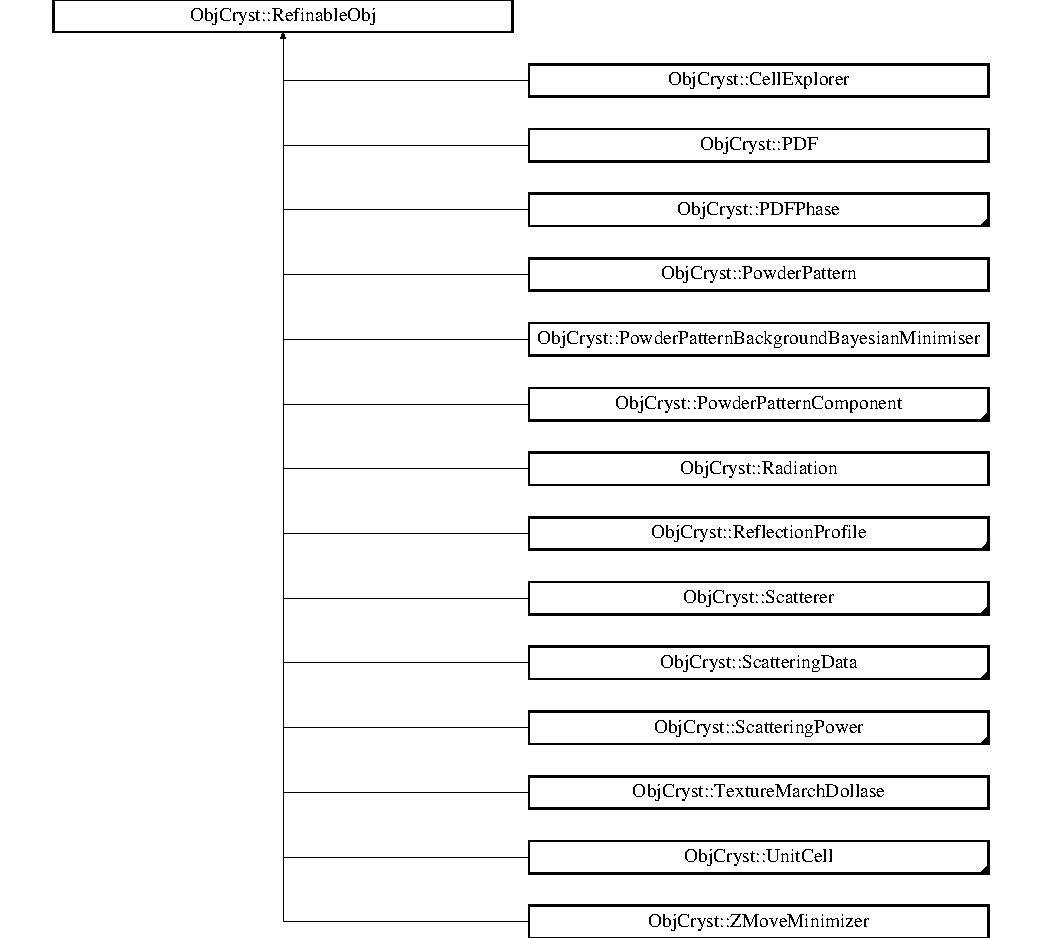
\includegraphics[height=12.000000cm]{a00077}
\end{center}
\end{figure}
\subsubsection*{Public Member Functions}
\begin{DoxyCompactItemize}
\item 
{\bf Refinable\-Obj} ()\label{a00077_a081d2bfc2065c2adaa2bfdf292900235}

\begin{DoxyCompactList}\small\item\em Constructor. \end{DoxyCompactList}\item 
{\bf Refinable\-Obj} (const bool internal\-Use\-Only)
\begin{DoxyCompactList}\small\item\em Constructor. \end{DoxyCompactList}\item 
{\bf Refinable\-Obj} (const {\bf Refinable\-Obj} \&old)
\begin{DoxyCompactList}\small\item\em Defined not implemented... \end{DoxyCompactList}\item 
virtual {\bf $\sim$\-Refinable\-Obj} ()\label{a00077_a5cd8d41a828153e2585077a9fbd334ce}

\begin{DoxyCompactList}\small\item\em Destructor. \end{DoxyCompactList}\item 
virtual const string \& {\bf Get\-Class\-Name} () const 
\begin{DoxyCompactList}\small\item\em Name for this class (\char`\"{}\-Refinable\-Obj\char`\"{}, \char`\"{}\-Crystal\char`\"{},...). \end{DoxyCompactList}\item 
virtual const string \& {\bf Get\-Name} () const \label{a00077_a61f51d3364e13a542e8c32df454c88aa}

\begin{DoxyCompactList}\small\item\em Name of the object. \end{DoxyCompactList}\item 
virtual void {\bf Set\-Name} (const string \&name)\label{a00077_a464caf574804fc21bd896f823131a1d7}

\begin{DoxyCompactList}\small\item\em Name of the object. \end{DoxyCompactList}\item 
void {\bf operator=} (const {\bf Refinable\-Obj} \&old)
\begin{DoxyCompactList}\small\item\em Defined not implemented... \end{DoxyCompactList}\item 
void {\bf Prepare\-For\-Refinement} () const 
\begin{DoxyCompactList}\small\item\em Find which parameters are used and {\bfseries not} fixed, for a refinement /optimization. \end{DoxyCompactList}\item 
void {\bf Fix\-All\-Par} ()\label{a00077_ac1a65da1f7563472badaf699002b8b8b}

\begin{DoxyCompactList}\small\item\em Fix All parameters. \end{DoxyCompactList}\item 
void {\bf Un\-Fix\-All\-Par} ()\label{a00077_ab75dcf763d7f96063dcb4d85e6e78007}

\begin{DoxyCompactList}\small\item\em Un\-Fix All parameters. \end{DoxyCompactList}\item 
void {\bf Set\-Par\-Is\-Fixed} (const long par\-Index, const bool fix)\label{a00077_ad6284ca6b92364e1ebd02bbef81d7e7e}

\begin{DoxyCompactList}\small\item\em Fix/un-\/fix one parameter from its \#. \end{DoxyCompactList}\item 
void {\bf Set\-Par\-Is\-Fixed} (const string \&par\-Name, const bool fix)\label{a00077_a8dc4cb100f839e12a9e0ae01facc5c9c}

\begin{DoxyCompactList}\small\item\em Fix/un-\/fix one parameter from its name. \end{DoxyCompactList}\item 
void {\bf Set\-Par\-Is\-Fixed} (const {\bf Ref\-Par\-Type} $\ast$type, const bool fix)\label{a00077_acc7f25893d4dc4cec08fd04a84aa008d}

\begin{DoxyCompactList}\small\item\em Fix/un-\/fix one family of parameters. \end{DoxyCompactList}\item 
void {\bf Set\-Par\-Is\-Used} (const string \&par\-Name, const bool use)\label{a00077_a1d0737a4ecb7cb1339f3138cd792ba7c}

\begin{DoxyCompactList}\small\item\em Set whether a parameter is used. \end{DoxyCompactList}\item 
void {\bf Set\-Par\-Is\-Used} (const {\bf Ref\-Par\-Type} $\ast$type, const bool use)\label{a00077_a40eba4b59117dd18831286e05b5b982c}

\begin{DoxyCompactList}\small\item\em Set whether a family of parameters is used. \end{DoxyCompactList}\item 
long {\bf Get\-Nb\-Par} () const 
\begin{DoxyCompactList}\small\item\em Total number of refinable parameter in the object. \end{DoxyCompactList}\item 
long {\bf Get\-Nb\-Par\-Not\-Fixed} () const \label{a00077_a6ead9da8785dbaa3dc4fb5f93cb455a3}

\begin{DoxyCompactList}\small\item\em Total number of non-\/fixed parameters. Is initialized by \doxyref{Prepare\-For\-Refinement()}{p.}{a00077_a0e9b816ad753f633ef6d9650ec6b4ca6} \end{DoxyCompactList}\item 
{\bf Refinable\-Par} \& {\bf Get\-Par} (const long i)\label{a00077_ae5c543d3b0fb010afa37b5f12620405b}

\begin{DoxyCompactList}\small\item\em Access all parameters in the order they were inputted. \end{DoxyCompactList}\item 
const {\bf Refinable\-Par} \& {\bf Get\-Par} (const long i) const \label{a00077_a5686cc39b27bc719be33aad0700438a1}

\begin{DoxyCompactList}\small\item\em Access all parameters in the order they were inputted. \end{DoxyCompactList}\item 
{\bf Refinable\-Par} \& {\bf Get\-Par} (const string \&name)\label{a00077_aea1c3b652c3f1eb5444bd47456e04392}

\begin{DoxyCompactList}\small\item\em Access all parameters from their name. \end{DoxyCompactList}\item 
const {\bf Refinable\-Par} \& {\bf Get\-Par} (const string \&name) const \label{a00077_a519b443c48cc463ed6b0682a6f557074}

\begin{DoxyCompactList}\small\item\em Access all parameters from their name. \end{DoxyCompactList}\item 
{\bf Refinable\-Par} \& {\bf Get\-Par} (const R\-E\-A\-L $\ast$)\label{a00077_a07ea375ae64f69559e0b595e8c111087}

\begin{DoxyCompactList}\small\item\em Access parameter from its adress. \end{DoxyCompactList}\item 
const {\bf Refinable\-Par} \& {\bf Get\-Par} (const R\-E\-A\-L $\ast$) const \label{a00077_a82b9eeedc157f76f17e9f9461c3a11d7}

\begin{DoxyCompactList}\small\item\em Access parameter from its adress. \end{DoxyCompactList}\item 
long {\bf Get\-Par\-Index} (const string \&name, const bool nothrow=false) const \label{a00077_ac226ae69247c59e1d22b5be5010534c9}

\begin{DoxyCompactList}\small\item\em Get a parameter index (the order it was inputted) from its name. \end{DoxyCompactList}\item 
long {\bf Get\-Par\-Index} (const R\-E\-A\-L $\ast$, const bool nothrow=false) const \label{a00077_a86afd7f55aafa42dd0a65a04c3eaf192}

\begin{DoxyCompactList}\small\item\em Get a parameter index (the order it was inputted) from its adress. \end{DoxyCompactList}\item 
{\bf Refinable\-Par} \& {\bf Get\-Par\-Not\-Fixed} (const long i)
\begin{DoxyCompactList}\small\item\em Access all parameters in the order they were inputted, skipping fixed parameters. \end{DoxyCompactList}\item 
const {\bf Refinable\-Par} \& {\bf Get\-Par\-Not\-Fixed} (const long i) const 
\begin{DoxyCompactList}\small\item\em Access all parameters in the order they were inputed, skipping fixed parameters. \end{DoxyCompactList}\item 
void {\bf Add\-Par} (const {\bf Refinable\-Par} \&new\-Ref\-Par)
\begin{DoxyCompactList}\small\item\em Add a refinable parameter. \end{DoxyCompactList}\item 
void {\bf Add\-Par} ({\bf Refinable\-Par} $\ast$new\-Ref\-Par)
\begin{DoxyCompactList}\small\item\em Add a refinable parameter. \end{DoxyCompactList}\item 
void {\bf Add\-Par} ({\bf Refinable\-Obj} \&new\-Ref\-Par\-List, const bool copy\-Param=false)
\begin{DoxyCompactList}\small\item\em Add all the parameters in another \doxyref{Refinable\-Obj}{p.}{a00077}. \end{DoxyCompactList}\item 
vector$<$ {\bf Refinable\-Par} $\ast$ $>$\-::iterator {\bf Remove\-Par} ({\bf Refinable\-Par} $\ast$ref\-Par)
\begin{DoxyCompactList}\small\item\em Remove a refinable parameter. \end{DoxyCompactList}\item 
virtual void {\bfseries Print} () const \label{a00077_a6033a7d7892806d9157daad9c4aea8c3}

\item 
unsigned long {\bf Create\-Param\-Set} (const string name=\char`\"{}\char`\"{}) const 
\begin{DoxyCompactList}\small\item\em Save the current set of refined values in a new set. \end{DoxyCompactList}\item 
void {\bf Clear\-Param\-Set} (const unsigned long id) const \label{a00077_ae9a2401becfcd7dda785c0931d3f31f3}

\begin{DoxyCompactList}\small\item\em Erase the param set with the given id, releasing memory. \end{DoxyCompactList}\item 
void {\bf Save\-Param\-Set} (const unsigned long id) const 
\begin{DoxyCompactList}\small\item\em Save the current set of refined values over a previously-\/created set of saved values. \end{DoxyCompactList}\item 
void {\bf Restore\-Param\-Set} (const unsigned long id)
\begin{DoxyCompactList}\small\item\em Restore a saved set of values. \end{DoxyCompactList}\item 
const Cryst\-Vector\-\_\-\-R\-E\-A\-L \& {\bf Get\-Param\-Set} (const unsigned long set\-Id) const 
\begin{DoxyCompactList}\small\item\em Access one save refpar set. \end{DoxyCompactList}\item 
Cryst\-Vector\-\_\-\-R\-E\-A\-L \& {\bf Get\-Param\-Set} (const unsigned long set\-Id)
\begin{DoxyCompactList}\small\item\em Access one save refpar set. \end{DoxyCompactList}\item 
R\-E\-A\-L {\bf Get\-Param\-Set\-\_\-\-Par\-Not\-Fixed\-Human\-Value} (const unsigned long set\-Id, const long par\-Number) const 
\begin{DoxyCompactList}\small\item\em Access the (human) value of one refined parameter in a saved set of parameters. \end{DoxyCompactList}\item 
const void {\bf Erase\-All\-Param\-Set} ()
\begin{DoxyCompactList}\small\item\em Erase all saved refpar sets. \end{DoxyCompactList}\item 
const string \& {\bf Get\-Param\-Set\-Name} (const unsigned long set\-Id) const 
\begin{DoxyCompactList}\small\item\em Get the name associated to a refpar set. \end{DoxyCompactList}\item 
void {\bf Set\-Limits\-Absolute} (const string \&par\-Name, const R\-E\-A\-L min, const R\-E\-A\-L max)\label{a00077_a2f24a7b834f5588e32aac9c6e33a1020}

\begin{DoxyCompactList}\small\item\em Change the limits for a given parameter, giving absolute new limits. \end{DoxyCompactList}\item 
void {\bf Set\-Limits\-Absolute} (const {\bf Ref\-Par\-Type} $\ast$type, const R\-E\-A\-L min, const R\-E\-A\-L max)\label{a00077_a371f137ad14a77ee3b545520d05fe4d6}

\begin{DoxyCompactList}\small\item\em Change the limits for a category of parameters, giving absolute new limits. \end{DoxyCompactList}\item 
void {\bf Set\-Limits\-Relative} (const string \&par\-Name, const R\-E\-A\-L min, const R\-E\-A\-L max)
\begin{DoxyCompactList}\small\item\em Change the limits for a given parameter, giving relative new limits (eg giving -\/.\-1 and +.1 will set new limits at the current value + min and current value + max) Thus min should logically be $<$0 and max $>$0. \end{DoxyCompactList}\item 
void {\bf Set\-Limits\-Relative} (const {\bf Ref\-Par\-Type} $\ast$type, const R\-E\-A\-L min, const R\-E\-A\-L max)
\begin{DoxyCompactList}\small\item\em Change the limits for a category of parameters, giving relative new limits (eg giving -\/.\-1 and +.1 will set new limits at the current value + min and current value + max). \end{DoxyCompactList}\item 
void {\bf Set\-Limits\-Proportional} (const string \&par\-Name, const R\-E\-A\-L min, const R\-E\-A\-L max)
\begin{DoxyCompactList}\small\item\em Change the limits for a given parameter, proportionnaly to the current value. \end{DoxyCompactList}\item 
void {\bf Set\-Limits\-Proportional} (const {\bf Ref\-Par\-Type} $\ast$type, const R\-E\-A\-L min, const R\-E\-A\-L max)
\begin{DoxyCompactList}\small\item\em Change the limits for a category of parameters, proportionnaly to their current value. \end{DoxyCompactList}\item 
void {\bf Set\-Global\-Optim\-Step} (const {\bf Ref\-Par\-Type} $\ast$type, const R\-E\-A\-L step)\label{a00077_ae4f0b5b0038ff3b49dcdc8adbf98bc58}

\begin{DoxyCompactList}\small\item\em Change the maximum step to use during Global Optimization algorithms. \end{DoxyCompactList}\item 
{\bf Obj\-Registry}$<$ {\bf Refinable\-Obj} $>$ \& {\bf Get\-Sub\-Obj\-Registry} ()\label{a00077_a30e81164b0176ca00e90d994ca0a0827}

\begin{DoxyCompactList}\small\item\em Access to the registry of \doxyref{Refinable\-Obj}{p.}{a00077} used by this object. \end{DoxyCompactList}\item 
const {\bf Obj\-Registry}$<$ {\bf Refinable\-Obj} $>$ \& {\bf Get\-Sub\-Obj\-Registry} () const \label{a00077_a23999d5fb06661cddc9bfa294c48624e}

\begin{DoxyCompactList}\small\item\em Access to the registry of \doxyref{Refinable\-Obj}{p.}{a00077} used by this object. \end{DoxyCompactList}\item 
virtual void {\bf Register\-Client} ({\bf Refinable\-Obj} \&) const 
\begin{DoxyCompactList}\small\item\em Register a new object using this object. \end{DoxyCompactList}\item 
virtual void {\bf De\-Register\-Client} ({\bf Refinable\-Obj} \&) const \label{a00077_ae37091ca0b7091eaf87bf630433ad91d}

\begin{DoxyCompactList}\small\item\em Deregister an object (which not any more) using this object. \end{DoxyCompactList}\item 
virtual const {\bf Obj\-Registry}\\*
$<$ {\bf Refinable\-Obj} $>$ \& {\bf Get\-Client\-Registry} () const \label{a00077_abb63797f2ffc7e8317f66ce9749f105f}

\begin{DoxyCompactList}\small\item\em Get the list of clients. \end{DoxyCompactList}\item 
virtual {\bf Obj\-Registry}\\*
$<$ {\bf Refinable\-Obj} $>$ \& {\bf Get\-Client\-Registry} ()\label{a00077_aaf7fdd5c8d015285639fe24138e31b6b}

\begin{DoxyCompactList}\small\item\em Get the list of clients. \end{DoxyCompactList}\item 
bool {\bf Is\-Being\-Refined} () const \label{a00077_addbd91121eaf715f67080d95cfdc857c}

\begin{DoxyCompactList}\small\item\em Is the object being refined ? (Can be refined by one algorithm at a time only.) \end{DoxyCompactList}\item 
virtual void {\bf Begin\-Optimization} (const bool allow\-Approximations=false, const bool enable\-Restraints=false)
\begin{DoxyCompactList}\small\item\em This should be called by any optimization class at the begining of an optimization. \end{DoxyCompactList}\item 
virtual void {\bf End\-Optimization} ()
\begin{DoxyCompactList}\small\item\em This should be called by any optimization class at the end of an optimization. \end{DoxyCompactList}\item 
virtual void {\bf Set\-Approximation\-Flag} (const bool allow)
\begin{DoxyCompactList}\small\item\em Enable or disable numerical approximations. \end{DoxyCompactList}\item 
virtual void {\bf Randomize\-Configuration} ()
\begin{DoxyCompactList}\small\item\em Randomize Configuration (before a global optimization). \end{DoxyCompactList}\item 
virtual void {\bf Global\-Opt\-Random\-Move} (const R\-E\-A\-L mutation\-Amplitude, const {\bf Ref\-Par\-Type} $\ast$type={\bf gp\-Ref\-Par\-Type\-Obj\-Cryst})
\begin{DoxyCompactList}\small\item\em Make a random move of the current configuration. \end{DoxyCompactList}\item 
void {\bf Begin\-Global\-Opt\-Random\-Move} ()
\begin{DoxyCompactList}\small\item\em Raise a flag, to be sure not to make a random change more than once in each \doxyref{Refinable\-Obj}{p.}{a00077}. \end{DoxyCompactList}\item 
virtual R\-E\-A\-L {\bf Get\-Log\-Likelihood} () const 
\begin{DoxyCompactList}\small\item\em Get -\/log(likelihood) of the current configuration for the object. \end{DoxyCompactList}\item 
virtual unsigned int {\bf Get\-Nb\-L\-S\-Q\-Function} () const \label{a00077_af435b8a23739f154222ba619f67cfc92}

\begin{DoxyCompactList}\small\item\em Number of L\-S\-Q functions. \end{DoxyCompactList}\item 
virtual const Cryst\-Vector\-\_\-\-R\-E\-A\-L \& {\bf Get\-L\-S\-Q\-Calc} (const unsigned int) const \label{a00077_a99e8e0a4d761829f940c0ed3d29fec89}

\begin{DoxyCompactList}\small\item\em Get the current calculated value for the L\-S\-Q function. \end{DoxyCompactList}\item 
virtual const Cryst\-Vector\-\_\-\-R\-E\-A\-L \& {\bf Get\-L\-S\-Q\-Obs} (const unsigned int) const \label{a00077_a60ecf8524c697c0385c3810b825459f2}

\begin{DoxyCompactList}\small\item\em Get the observed values for the L\-S\-Q function. \end{DoxyCompactList}\item 
virtual const Cryst\-Vector\-\_\-\-R\-E\-A\-L \& {\bf Get\-L\-S\-Q\-Weight} (const unsigned int) const \label{a00077_a798d3ab37d696395897a0a416f0757c0}

\begin{DoxyCompactList}\small\item\em Get the weight values for the L\-S\-Q function. \end{DoxyCompactList}\item 
virtual const Cryst\-Vector\-\_\-\-R\-E\-A\-L \& {\bf Get\-L\-S\-Q\-Deriv} (const unsigned int, {\bf Refinable\-Par} \&)
\begin{DoxyCompactList}\small\item\em Get the first derivative values for the L\-S\-Q function, for a given parameter. \end{DoxyCompactList}\item 
void {\bf Reset\-Par\-List} ()
\begin{DoxyCompactList}\small\item\em Re-\/init the list of refinable parameters, removing all parameters. \end{DoxyCompactList}\item 
virtual void {\bf X\-M\-L\-Output} (ostream \&os, int indent=0) const 
\begin{DoxyCompactList}\small\item\em Output to stream in well-\/formed X\-M\-L. \end{DoxyCompactList}\item 
virtual void {\bf X\-M\-L\-Input} (istream \&is, const {\bf X\-M\-L\-Cryst\-Tag} \&tag)
\begin{DoxyCompactList}\small\item\em Input From stream. \end{DoxyCompactList}\item 
virtual void {\bf Update\-Display} () const 
\begin{DoxyCompactList}\small\item\em If there is an interface, this should be automatically be called each time there is a 'new, significant' configuration to report. \end{DoxyCompactList}\item 
unsigned int {\bf Get\-Nb\-Option} () const \label{a00077_a389c9d9ed7e8c700abfa4dfb72a32792}

\begin{DoxyCompactList}\small\item\em Number of Options for this object. \end{DoxyCompactList}\item 
{\bf Ref\-Obj\-Opt} \& {\bf Get\-Option} (const unsigned int i)\label{a00077_a2dcb69d78e55dc75a7377e5a772536de}

\begin{DoxyCompactList}\small\item\em Access to the options. \end{DoxyCompactList}\item 
const {\bf Ref\-Obj\-Opt} \& {\bf Get\-Option} (const unsigned int i) const \label{a00077_a77b66fd9c4e752e9b58ecd9e5ec2a218}

\begin{DoxyCompactList}\small\item\em const access to the options \end{DoxyCompactList}\item 
virtual void {\bf Get\-Gene\-Group} (const {\bf Refinable\-Obj} \&obj, Cryst\-Vector\-\_\-uint \&group\-Index, unsigned int \&first\-Group) const 
\begin{DoxyCompactList}\small\item\em Get the gene group assigned to each parameter. \end{DoxyCompactList}\item 
void {\bf Set\-Delete\-Ref\-Par\-In\-Destructor} (const bool b)
\begin{DoxyCompactList}\small\item\em Set this object not to delete its list of parameters when destroyed. \end{DoxyCompactList}\item 
const {\bf Refinable\-Obj\-Clock} \& {\bf Get\-Ref\-Par\-List\-Clock} () const 
\begin{DoxyCompactList}\small\item\em What was the last time a \doxyref{Refinable\-Par}{p.}{a00079} was added/removed ? \end{DoxyCompactList}\item 
virtual R\-E\-A\-L {\bf Get\-Restraint\-Cost} () const 
\begin{DoxyCompactList}\small\item\em Get the restraint cost (overall penalty of all restraints) \end{DoxyCompactList}\item 
void {\bf Add\-Restraint} ({\bf Restraint} $\ast$p\-New\-Restraint)
\begin{DoxyCompactList}\small\item\em Add a new restraint. \end{DoxyCompactList}\item 
vector$<$ {\bf Restraint} $\ast$ $>$\-::iterator {\bf Remove\-Restraint} ({\bf Restraint} $\ast$p\-Restraint)
\begin{DoxyCompactList}\small\item\em Remove a restraint from the list of known restraints. \end{DoxyCompactList}\item 
virtual void {\bf Tag\-New\-Best\-Config} () const 
\begin{DoxyCompactList}\small\item\em During a global optimization, tells the object that the current config is the latest \char`\"{}best\char`\"{} config. \end{DoxyCompactList}\item 
const {\bf Refinable\-Obj\-Clock} \& {\bf Get\-Clock\-Master} () const \label{a00077_a5910fb213a6b51da18d5f65badceb029}

\begin{DoxyCompactList}\small\item\em This clocks records {\itshape any} change in the object. See refinable\-Obj\-::m\-Clock\-Master. \end{DoxyCompactList}\end{DoxyCompactItemize}
\subsubsection*{Protected Member Functions}
\begin{DoxyCompactItemize}
\item 
long {\bf Find\-Par} (const string \&name) const \label{a00077_a6c1fd4ec11915278a6a9db9bf3aa1374}

\begin{DoxyCompactList}\small\item\em Find a refinable parameter with a given name. \end{DoxyCompactList}\item 
long {\bf Find\-Par} (const R\-E\-A\-L $\ast$) const \label{a00077_a96acb0979c364332bc5365a73b58a246}

\begin{DoxyCompactList}\small\item\em Find a refinable parameter from the adress of its value. \end{DoxyCompactList}\item 
void {\bf Add\-Sub\-Ref\-Obj} ({\bf Refinable\-Obj} \&)
\item 
void {\bf Remove\-Sub\-Ref\-Obj} ({\bf Refinable\-Obj} \&)
\item 
void {\bf Add\-Option} ({\bf Ref\-Obj\-Opt} $\ast$opt)
\item 
virtual void {\bf Prepare} ()
\item 
map$<$ unsigned long, pair\\*
$<$ Cryst\-Vector\-\_\-\-R\-E\-A\-L, string $>$\\*
 $>$\-::iterator {\bf Find\-Param\-Set} (unsigned long id) const \label{a00077_a5db8d488c4782f2e143fbb6ec96e0b32}

\begin{DoxyCompactList}\small\item\em Find a parameter set with a given id (and check if it is there) \end{DoxyCompactList}\end{DoxyCompactItemize}
\subsubsection*{Protected Attributes}
\begin{DoxyCompactItemize}
\item 
string {\bf m\-Name}\label{a00077_ad8ddc8c4b3daae8649986d7febc5fca4}

\begin{DoxyCompactList}\small\item\em Name for this Refinable\-Object. Should be unique, at least in the same scope.+. \end{DoxyCompactList}\item 
vector$<$ {\bf Refinable\-Par} $\ast$ $>$ {\bf mvp\-Ref\-Par}\label{a00077_ae05556c30ef2d6818c22750c89690fc9}

\begin{DoxyCompactList}\small\item\em Vector of pointers to the refinable parameters. \end{DoxyCompactList}\item 
vector$<$ {\bf Restraint} $\ast$ $>$ {\bf mvp\-Restraint}
\begin{DoxyCompactList}\small\item\em Vector of pointers to the restraints for this object. \end{DoxyCompactList}\item 
map$<$ unsigned long, pair\\*
$<$ Cryst\-Vector\-\_\-\-R\-E\-A\-L, string $>$ $>$ {\bf mvp\-Saved\-Values\-Set}
\begin{DoxyCompactList}\small\item\em Map of (index,pointers to arrays) used to save sets of values for all parameters. \end{DoxyCompactList}\item 
long {\bf m\-Nb\-Ref\-Par\-Not\-Fixed}\label{a00077_a8cffff9a5b5d2a76bd9e29cce5f4700e}

\begin{DoxyCompactList}\small\item\em Total of not-\/fixed parameters. \end{DoxyCompactList}\item 
Cryst\-Vector\-\_\-long {\bf m\-Refpar\-Not\-Fixed\-Index}\label{a00077_a359f6599fdaa11ea01afd91289265bac}

\begin{DoxyCompactList}\small\item\em Index of not-\/fixed parameters. \end{DoxyCompactList}\item 
int {\bf m\-Optimization\-Depth}
\begin{DoxyCompactList}\small\item\em Is the object being refined or optimized ? if m\-Optimization\-Depth=0, no optimization is taking place. \end{DoxyCompactList}\item 
{\bf Obj\-Registry}$<$ {\bf Refinable\-Obj} $>$ {\bf m\-Sub\-Obj\-Registry}\label{a00077_a101ff2559ab840729c8cbc7b2469afd6}

\begin{DoxyCompactList}\small\item\em Registry of Refinable\-Object needed for this object (owned by this object or not) \end{DoxyCompactList}\item 
{\bf Obj\-Registry}$<$ {\bf Refinable\-Obj} $>$ {\bf m\-Client\-Obj\-Registry}
\begin{DoxyCompactList}\small\item\em Registry of Refinable\-Object using this object. \end{DoxyCompactList}\item 
{\bf Obj\-Registry}$<$ {\bf Ref\-Obj\-Opt} $>$ {\bf m\-Option\-Registry}
\begin{DoxyCompactList}\small\item\em List of options for this object. \end{DoxyCompactList}\item 
bool {\bf m\-Delete\-Ref\-Par\-In\-Destructor}
\begin{DoxyCompactList}\small\item\em If true (the default), then all \doxyref{Refinable\-Par}{p.}{a00079} will be deleted when the the object is deleted. \end{DoxyCompactList}\item 
{\bf Refinable\-Obj\-Clock} {\bf m\-Ref\-Par\-List\-Clock}\label{a00077_a867562fcd8c5afd0fd178c98729e1f35}

\begin{DoxyCompactList}\small\item\em Last time the Refinable\-Par\-List was modified (a parameter added or removed). \end{DoxyCompactList}\item 
bool {\bf m\-Random\-Move\-Is\-Done}
\item 
Cryst\-Vector\-\_\-\-R\-E\-A\-L {\bf m\-L\-S\-Q\-Deriv}
\begin{DoxyCompactList}\small\item\em Temporary array used to return derivative values of the L\-S\-Q function for given parameters. \end{DoxyCompactList}\item 
{\bf Refinable\-Obj\-Clock} {\bf m\-Clock\-Master}
\begin{DoxyCompactList}\small\item\em Master clock, which is changed whenever the object has been altered. \end{DoxyCompactList}\end{DoxyCompactItemize}


\subsubsection{Detailed Description}
Generic Refinable Object. 

This is basically a list of refinable parameters, with other basic common properties such as a name,. etc... This allows optimization/refinement algorithms to access the parameters without knowing what the object really is.

\begin{DoxyRefDesc}{Todo}
\item[{\bf Todo}]Define more clearly which operations are recursive (ie also modify sub-\/objects). \end{DoxyRefDesc}


\subsubsection{Constructor \& Destructor Documentation}
\index{Obj\-Cryst\-::\-Refinable\-Obj@{Obj\-Cryst\-::\-Refinable\-Obj}!Refinable\-Obj@{Refinable\-Obj}}
\index{Refinable\-Obj@{Refinable\-Obj}!ObjCryst::RefinableObj@{Obj\-Cryst\-::\-Refinable\-Obj}}
\paragraph[{Refinable\-Obj}]{\setlength{\rightskip}{0pt plus 5cm}Obj\-Cryst\-::\-Refinable\-Obj\-::\-Refinable\-Obj (
\begin{DoxyParamCaption}
\item[{const bool}]{internal\-Use\-Only}
\end{DoxyParamCaption}
)}\label{a00077_aa0eaf0982686476cbec02a8afeebc92d}


Constructor. 

Using internal\-Use\-Only=true will avoid registering the the object to any registry, and thus (for example) no display will be created, nor will this object be automatically be saved. \index{Obj\-Cryst\-::\-Refinable\-Obj@{Obj\-Cryst\-::\-Refinable\-Obj}!Refinable\-Obj@{Refinable\-Obj}}
\index{Refinable\-Obj@{Refinable\-Obj}!ObjCryst::RefinableObj@{Obj\-Cryst\-::\-Refinable\-Obj}}
\paragraph[{Refinable\-Obj}]{\setlength{\rightskip}{0pt plus 5cm}Obj\-Cryst\-::\-Refinable\-Obj\-::\-Refinable\-Obj (
\begin{DoxyParamCaption}
\item[{const {\bf Refinable\-Obj} \&}]{old}
\end{DoxyParamCaption}
)}\label{a00077_a5f77dcf037cc8d2ea1fd84bfda6ddbc0}


Defined not implemented... 

Should never be called (copying the refinable parameters would allow you to modify the input object). Use the default constructor and Refinable\-Obj\-::\-Add\-Par(\-Refinable\-Obj\&) instead. 

\subsubsection{Member Function Documentation}
\index{Obj\-Cryst\-::\-Refinable\-Obj@{Obj\-Cryst\-::\-Refinable\-Obj}!Add\-Option@{Add\-Option}}
\index{Add\-Option@{Add\-Option}!ObjCryst::RefinableObj@{Obj\-Cryst\-::\-Refinable\-Obj}}
\paragraph[{Add\-Option}]{\setlength{\rightskip}{0pt plus 5cm}void Obj\-Cryst\-::\-Refinable\-Obj\-::\-Add\-Option (
\begin{DoxyParamCaption}
\item[{{\bf Ref\-Obj\-Opt} $\ast$}]{opt}
\end{DoxyParamCaption}
)\hspace{0.3cm}{\ttfamily [protected]}}\label{a00077_a8bd8353b34fc4088a987be0eaf01e5f6}
Add an option for this parameter \index{Obj\-Cryst\-::\-Refinable\-Obj@{Obj\-Cryst\-::\-Refinable\-Obj}!Add\-Par@{Add\-Par}}
\index{Add\-Par@{Add\-Par}!ObjCryst::RefinableObj@{Obj\-Cryst\-::\-Refinable\-Obj}}
\paragraph[{Add\-Par}]{\setlength{\rightskip}{0pt plus 5cm}void Obj\-Cryst\-::\-Refinable\-Obj\-::\-Add\-Par (
\begin{DoxyParamCaption}
\item[{const {\bf Refinable\-Par} \&}]{new\-Ref\-Par}
\end{DoxyParamCaption}
)}\label{a00077_a0c0050a3d3141ca34eb8f4b559ad2f8d}


Add a refinable parameter. 

The parameter is copied, so it need only be allocated temporarily.

\begin{DoxyRefDesc}{Deprecated}
\item[{\bf Deprecated}]Use the next function, which supplies the parameter as a pointer, and avoids a useless copy. \begin{DoxyNote}{Note}
\-: if a parameter is added and its name is already used by another, its name will be automatically appended with an $\sim$ 
\end{DoxyNote}
\end{DoxyRefDesc}
\index{Obj\-Cryst\-::\-Refinable\-Obj@{Obj\-Cryst\-::\-Refinable\-Obj}!Add\-Par@{Add\-Par}}
\index{Add\-Par@{Add\-Par}!ObjCryst::RefinableObj@{Obj\-Cryst\-::\-Refinable\-Obj}}
\paragraph[{Add\-Par}]{\setlength{\rightskip}{0pt plus 5cm}void Obj\-Cryst\-::\-Refinable\-Obj\-::\-Add\-Par (
\begin{DoxyParamCaption}
\item[{{\bf Refinable\-Par} $\ast$}]{new\-Ref\-Par}
\end{DoxyParamCaption}
)}\label{a00077_a4a792c84f7d35e71b3e89aae5a87bffa}


Add a refinable parameter. 

The parameter is {\itshape not} copied, so it should be allocated in the heap.

\begin{DoxyNote}{Note}
\-: if a parameter is added and its name is already used by another, its name will be automatically appended with an $\sim$ 
\end{DoxyNote}
\index{Obj\-Cryst\-::\-Refinable\-Obj@{Obj\-Cryst\-::\-Refinable\-Obj}!Add\-Par@{Add\-Par}}
\index{Add\-Par@{Add\-Par}!ObjCryst::RefinableObj@{Obj\-Cryst\-::\-Refinable\-Obj}}
\paragraph[{Add\-Par}]{\setlength{\rightskip}{0pt plus 5cm}void Obj\-Cryst\-::\-Refinable\-Obj\-::\-Add\-Par (
\begin{DoxyParamCaption}
\item[{{\bf Refinable\-Obj} \&}]{new\-Ref\-Par\-List, }
\item[{const bool}]{copy\-Param = {\ttfamily false}}
\end{DoxyParamCaption}
)}\label{a00077_a6a28259e473fadd53fbc9b9bf7930813}


Add all the parameters in another \doxyref{Refinable\-Obj}{p.}{a00077}. 

Parameters are  copied, so they should be allocated in the heap.

\begin{DoxyWarning}{Warning}
If a copy of another \doxyref{Refinable\-Obj}{p.}{a00077} parameter list is made, such as in the \doxyref{Optimization\-Obj}{p.}{a00061} class, make sure that upon deletion of this object the parameters will not be destroyed. To do this use Refinable\-Obj\-::\-Set\-Delete\-Ref\-Par\-In\-Destructor(false).
\end{DoxyWarning}

\begin{DoxyParams}{Parameters}
{\em copy\-Param} & if false (default), then parameters are not copied from the object but just referenced. Use Refinable\-Obj\-::\-Set\-Delete\-Ref\-Par\-In\-Destructor(false) accordingly. If true, then the parameters are copied, so that any modification to the fixed/limited/used attributes do not affect the original parameter. Only the value and the parameter's clock can then be modified by the copied parameter\\
\hline
\end{DoxyParams}
\begin{DoxyNote}{Note}
\-: if a parameter is added and its name is already used by another, its name will be automatically appended with an $\sim$ 
\end{DoxyNote}
\index{Obj\-Cryst\-::\-Refinable\-Obj@{Obj\-Cryst\-::\-Refinable\-Obj}!Add\-Restraint@{Add\-Restraint}}
\index{Add\-Restraint@{Add\-Restraint}!ObjCryst::RefinableObj@{Obj\-Cryst\-::\-Refinable\-Obj}}
\paragraph[{Add\-Restraint}]{\setlength{\rightskip}{0pt plus 5cm}void Obj\-Cryst\-::\-Refinable\-Obj\-::\-Add\-Restraint (
\begin{DoxyParamCaption}
\item[{{\bf Restraint} $\ast$}]{p\-New\-Restraint}
\end{DoxyParamCaption}
)}\label{a00077_a0eec1ccf5ba9769e5c6a82a85ecf451d}


Add a new restraint. 

This returns an iterator pointing to the next \doxyref{Restraint}{p.}{a00087} in the vector. \index{Obj\-Cryst\-::\-Refinable\-Obj@{Obj\-Cryst\-::\-Refinable\-Obj}!Add\-Sub\-Ref\-Obj@{Add\-Sub\-Ref\-Obj}}
\index{Add\-Sub\-Ref\-Obj@{Add\-Sub\-Ref\-Obj}!ObjCryst::RefinableObj@{Obj\-Cryst\-::\-Refinable\-Obj}}
\paragraph[{Add\-Sub\-Ref\-Obj}]{\setlength{\rightskip}{0pt plus 5cm}void Obj\-Cryst\-::\-Refinable\-Obj\-::\-Add\-Sub\-Ref\-Obj (
\begin{DoxyParamCaption}
\item[{{\bf Refinable\-Obj} \&}]{}
\end{DoxyParamCaption}
)\hspace{0.3cm}{\ttfamily [protected]}}\label{a00077_ae4740b33ea934e4ab9b9bce9ebbfa806}
Add an object in the registry of used objects. \index{Obj\-Cryst\-::\-Refinable\-Obj@{Obj\-Cryst\-::\-Refinable\-Obj}!Begin\-Global\-Opt\-Random\-Move@{Begin\-Global\-Opt\-Random\-Move}}
\index{Begin\-Global\-Opt\-Random\-Move@{Begin\-Global\-Opt\-Random\-Move}!ObjCryst::RefinableObj@{Obj\-Cryst\-::\-Refinable\-Obj}}
\paragraph[{Begin\-Global\-Opt\-Random\-Move}]{\setlength{\rightskip}{0pt plus 5cm}void Obj\-Cryst\-::\-Refinable\-Obj\-::\-Begin\-Global\-Opt\-Random\-Move (
\begin{DoxyParamCaption}
{}
\end{DoxyParamCaption}
)}\label{a00077_a47fc5a85493671a3590ed7e3971b18fe}


Raise a flag, to be sure not to make a random change more than once in each \doxyref{Refinable\-Obj}{p.}{a00077}. 

This calls recursively all sub-\/objects.

This is necessary since one object may be included in several others. This must be called before making a random configuration change on a list of objects. \index{Obj\-Cryst\-::\-Refinable\-Obj@{Obj\-Cryst\-::\-Refinable\-Obj}!Begin\-Optimization@{Begin\-Optimization}}
\index{Begin\-Optimization@{Begin\-Optimization}!ObjCryst::RefinableObj@{Obj\-Cryst\-::\-Refinable\-Obj}}
\paragraph[{Begin\-Optimization}]{\setlength{\rightskip}{0pt plus 5cm}virtual void Obj\-Cryst\-::\-Refinable\-Obj\-::\-Begin\-Optimization (
\begin{DoxyParamCaption}
\item[{const bool}]{allow\-Approximations = {\ttfamily false}, }
\item[{const bool}]{enable\-Restraints = {\ttfamily false}}
\end{DoxyParamCaption}
)\hspace{0.3cm}{\ttfamily [virtual]}}\label{a00077_ababd8f2916e41a20d2c1b21f6ffefe96}


This should be called by any optimization class at the begining of an optimization. 

This will also check that everything is ready, eg call the \doxyref{Refinable\-Obj\-::\-Prepare()}{p.}{a00077_a48d11671e7f8699f7bc24077585c5e0f} function. This also affects all sub-\/objects. \begin{DoxyNote}{Note}
this may be called several time for some objects which are used by several other objects, or for nested optimizations (e.\-g. least-\/squares optimizations inside a global one).

\doxyref{End\-Optimization()}{p.}{a00077_ab0035f6164cb24ace67b51b11993a851} must be called at the end of the optimization, the same number of time \doxyref{Begin\-Optimization()}{p.}{a00077_ababd8f2916e41a20d2c1b21f6ffefe96} was called !
\end{DoxyNote}

\begin{DoxyParams}{Parameters}
{\em allow\-Approximations} & if true, then the object can use faster but less precise functions during the optimization. This is useful for global optimization not using derivatives. \\
\hline
{\em enable\-Restraints\-:\textbackslash{}xrefitem} & deprecated 28. \\
\hline
\end{DoxyParams}


Reimplemented in {\bf Obj\-Cryst\-::\-Powder\-Pattern} \doxyref{}{p.}{a00068_a8e29b6186253d686c4f078906592df7b}, {\bf Obj\-Cryst\-::\-Molecule} \doxyref{}{p.}{a00053_a5fbdadb37966f382a6e33150285819dc}, {\bf Obj\-Cryst\-::\-Scattering\-Data} \doxyref{}{p.}{a00095_a6b0f18996edafa21a03bf9550dcf8981}, {\bf Obj\-Cryst\-::\-Powder\-Pattern\-Diffraction} \doxyref{}{p.}{a00072_a44d10a7c3404153fe4513c8944629c45}, {\bf Obj\-Cryst\-::\-Crystal} \doxyref{}{p.}{a00026_afe25ea6d287d6dd9cd0a03aed3798525}, {\bf Obj\-Cryst\-::\-Cell\-Explorer} \doxyref{}{p.}{a00020_ae75ee0eb6652d5d43404b7205ec3cb94}, {\bf Obj\-Cryst\-::\-Powder\-Pattern\-Background} \doxyref{}{p.}{a00069_ac9a022b49d583e8ae81e4d96e50cc9d8}, and {\bf Obj\-Cryst\-::\-Texture\-March\-Dollase} \doxyref{}{p.}{a00110_a73f6148d035bbdeb98b0115d76fe48a8}.

\index{Obj\-Cryst\-::\-Refinable\-Obj@{Obj\-Cryst\-::\-Refinable\-Obj}!Create\-Param\-Set@{Create\-Param\-Set}}
\index{Create\-Param\-Set@{Create\-Param\-Set}!ObjCryst::RefinableObj@{Obj\-Cryst\-::\-Refinable\-Obj}}
\paragraph[{Create\-Param\-Set}]{\setlength{\rightskip}{0pt plus 5cm}unsigned long Obj\-Cryst\-::\-Refinable\-Obj\-::\-Create\-Param\-Set (
\begin{DoxyParamCaption}
\item[{const string}]{name = {\ttfamily \char`\"{}\char`\"{}}}
\end{DoxyParamCaption}
) const}\label{a00077_abd5b0aa78ff6ec95838e78e2d3685b56}


Save the current set of refined values in a new set. 


\begin{DoxyParams}{Parameters}
{\em name} & \-: the name associated to this set of values. Names should be unique. \\
\hline
\end{DoxyParams}
\begin{DoxyReturn}{Returns}
an number identifying the set of saved values.
\end{DoxyReturn}
\begin{DoxyWarning}{Warning}
\-: there is no limit to the number of parameters sets, so try to release them when you don't need them. 
\end{DoxyWarning}
\index{Obj\-Cryst\-::\-Refinable\-Obj@{Obj\-Cryst\-::\-Refinable\-Obj}!End\-Optimization@{End\-Optimization}}
\index{End\-Optimization@{End\-Optimization}!ObjCryst::RefinableObj@{Obj\-Cryst\-::\-Refinable\-Obj}}
\paragraph[{End\-Optimization}]{\setlength{\rightskip}{0pt plus 5cm}virtual void Obj\-Cryst\-::\-Refinable\-Obj\-::\-End\-Optimization (
\begin{DoxyParamCaption}
{}
\end{DoxyParamCaption}
)\hspace{0.3cm}{\ttfamily [virtual]}}\label{a00077_ab0035f6164cb24ace67b51b11993a851}


This should be called by any optimization class at the end of an optimization. 

This also affects all sub-\/objects. \begin{DoxyNote}{Note}
this may be called several time for some objects which are used by several other objects. 
\end{DoxyNote}


Reimplemented in {\bf Obj\-Cryst\-::\-Molecule} \doxyref{}{p.}{a00053_aec0a3ba0d08fdfed38cc757efb635ffb}, {\bf Obj\-Cryst\-::\-Scattering\-Data} \doxyref{}{p.}{a00095_a782e0caf5c6f2941ca64d17293b1e8b4}, {\bf Obj\-Cryst\-::\-Powder\-Pattern\-Diffraction} \doxyref{}{p.}{a00072_a11f7690878a07983de3abb839b087798}, and {\bf Obj\-Cryst\-::\-Z\-Scatterer} \doxyref{}{p.}{a00162_a5742d1fa13b1300c92359ef1250753c3}.

\index{Obj\-Cryst\-::\-Refinable\-Obj@{Obj\-Cryst\-::\-Refinable\-Obj}!Erase\-All\-Param\-Set@{Erase\-All\-Param\-Set}}
\index{Erase\-All\-Param\-Set@{Erase\-All\-Param\-Set}!ObjCryst::RefinableObj@{Obj\-Cryst\-::\-Refinable\-Obj}}
\paragraph[{Erase\-All\-Param\-Set}]{\setlength{\rightskip}{0pt plus 5cm}const void Obj\-Cryst\-::\-Refinable\-Obj\-::\-Erase\-All\-Param\-Set (
\begin{DoxyParamCaption}
{}
\end{DoxyParamCaption}
)}\label{a00077_ac269ad4ad4ca8b4e9f13f5466475d959}


Erase all saved refpar sets. 

\index{Obj\-Cryst\-::\-Refinable\-Obj@{Obj\-Cryst\-::\-Refinable\-Obj}!Get\-Class\-Name@{Get\-Class\-Name}}
\index{Get\-Class\-Name@{Get\-Class\-Name}!ObjCryst::RefinableObj@{Obj\-Cryst\-::\-Refinable\-Obj}}
\paragraph[{Get\-Class\-Name}]{\setlength{\rightskip}{0pt plus 5cm}virtual const string\& Obj\-Cryst\-::\-Refinable\-Obj\-::\-Get\-Class\-Name (
\begin{DoxyParamCaption}
{}
\end{DoxyParamCaption}
) const\hspace{0.3cm}{\ttfamily [virtual]}}\label{a00077_a62968d90a7a3080738b363934616c019}


Name for this class (\char`\"{}\-Refinable\-Obj\char`\"{}, \char`\"{}\-Crystal\char`\"{},...). 

This is only useful to distinguish different classes when picking up objects from the \doxyref{Refinable\-Obj}{p.}{a00077} Global Registry 

Reimplemented in {\bf Obj\-Cryst\-::\-Molecule} \doxyref{}{p.}{a00053_a7f0f1ae6670032f5afc9ccf65d45f8c4}, {\bf Obj\-Cryst\-::\-Powder\-Pattern} \doxyref{}{p.}{a00068_a20dadada4d5b428c5122d4c75fb49164}, {\bf Obj\-Cryst\-::\-Scattering\-Power\-Atom} \doxyref{}{p.}{a00097_a87fcc8fe4871d1b9b6ec08af5f353657}, {\bf Obj\-Cryst\-::\-Powder\-Pattern\-Diffraction} \doxyref{}{p.}{a00072_a74b02e35219c6bc18521e66719778881}, {\bf Obj\-Cryst\-::\-Cell\-Explorer} \doxyref{}{p.}{a00020_a67ec6642b2a93030878764091178a0fb}, {\bf Obj\-Cryst\-::\-Z\-Scatterer} \doxyref{}{p.}{a00162_a610a62c221ed289e1ce4d68adac921ee}, {\bf Obj\-Cryst\-::\-Radiation} \doxyref{}{p.}{a00075_a56558c41ec3bd350a2904f5e469fb68a}, {\bf Obj\-Cryst\-::\-Powder\-Pattern\-Background} \doxyref{}{p.}{a00069_afae084513270b7adf50954bec4037380}, {\bf Obj\-Cryst\-::\-Reflection\-Profile\-Double\-Exponential\-Pseudo\-Voigt} \doxyref{}{p.}{a00081_a5e921c0682e78188e422c006e34df8a0}, {\bf Obj\-Cryst\-::\-Texture\-March\-Dollase} \doxyref{}{p.}{a00110_a2b1002c1ed071f53b2a6f1b953527cc2}, {\bf Obj\-Cryst\-::\-Scatterer} \doxyref{}{p.}{a00091_a374fc1bb2887ab1f61d456326d97c05f}, {\bf Obj\-Cryst\-::\-Crystal} \doxyref{}{p.}{a00026_ad1f69a5fb8981a2cf0eeb6245728af6d}, {\bf Obj\-Cryst\-::\-Scattering\-Power} \doxyref{}{p.}{a00096_ac31cc4135011046f93d49f4173aee3ee}, {\bf Obj\-Cryst\-::\-Reflection\-Profile\-Pseudo\-Voigt} \doxyref{}{p.}{a00082_a55628cdadc249b7973f2a6471d478e76}, {\bf Obj\-Cryst\-::\-Unit\-Cell} \doxyref{}{p.}{a00116_ac3b3c2e007083bf6f329eb11a6b610d1}, {\bf Obj\-Cryst\-::\-Atom} \doxyref{}{p.}{a00014_a9f0d1cb7c3b1db1baf84076e5da0ca0e}, {\bf Obj\-Cryst\-::\-Diffraction\-Data\-Single\-Crystal} \doxyref{}{p.}{a00032_a05b1f448a143ad61036f001d09a3509f}, {\bf Obj\-Cryst\-::\-Scattering\-Power\-Sphere} \doxyref{}{p.}{a00098_a57e85d29926fe93da66041a43583e893}, {\bf Obj\-Cryst\-::\-P\-D\-F} \doxyref{}{p.}{a00062_a809ab3f4cc8bdd268bd815baedccdc20}, {\bf Obj\-Cryst\-::\-Powder\-Pattern\-Component} \doxyref{}{p.}{a00071_a5e797476d8d76ef797e1e8b51db9e8fb}, and {\bf Obj\-Cryst\-::\-Powder\-Pattern\-Background\-Bayesian\-Minimiser} \doxyref{}{p.}{a00070_a7f39f799fafc12a3bdb937b5cc9545ad}.

\index{Obj\-Cryst\-::\-Refinable\-Obj@{Obj\-Cryst\-::\-Refinable\-Obj}!Get\-Gene\-Group@{Get\-Gene\-Group}}
\index{Get\-Gene\-Group@{Get\-Gene\-Group}!ObjCryst::RefinableObj@{Obj\-Cryst\-::\-Refinable\-Obj}}
\paragraph[{Get\-Gene\-Group}]{\setlength{\rightskip}{0pt plus 5cm}virtual void Obj\-Cryst\-::\-Refinable\-Obj\-::\-Get\-Gene\-Group (
\begin{DoxyParamCaption}
\item[{const {\bf Refinable\-Obj} \&}]{obj, }
\item[{Cryst\-Vector\-\_\-uint \&}]{group\-Index, }
\item[{unsigned int \&}]{first\-Group}
\end{DoxyParamCaption}
) const\hspace{0.3cm}{\ttfamily [virtual]}}\label{a00077_ad59c8ad2b0d7ee59fa3f399a54f05e54}


Get the gene group assigned to each parameter. 

Each parameter (a {\itshape gene} in terms of genetic algorithms) can be assigned to a gene group. Thus when mating two configurations, genes will be exchanged by groups. By default (in the base Refinabe\-Obj class), each parameter is alone in its group. Derived classes can group genes for a better s$\ast$$\ast$ life.

The number identifying a gene group only has a meaning in a given object. It can also change on subsequent calls, and thus is not unique.


\begin{DoxyParams}{Parameters}
{\em obj} & the , supplied by an algorithm class (\doxyref{Optimization\-Obj}{p.}{a00061},..), which contains a list of parameters, some of which (but possibly all or none) are parameters belonging to this object. \\
\hline
{\em group\-Index} & a vector of unsigned integers, one for each parameter in the input object, giving an unsigned integer value as gene group index. At the beginning this vector should contain only zeros (no group assigned). \\
\hline
{\em first\-Group} & this is the number of groups which have already been assigned, plus one. The gene groups returned by this object will start from this value, and increment {\bfseries first\-Group} for each gene group used, so that different \doxyref{Refinable\-Obj}{p.}{a00077} cannot share a gene group. \\
\hline
\end{DoxyParams}
\begin{DoxyNote}{Note}
this function is not optimized, and should only be called at the beginning of a refinement. 
\end{DoxyNote}


Reimplemented in {\bf Obj\-Cryst\-::\-Powder\-Pattern} \doxyref{}{p.}{a00068_ad3b643041cc61a3d39765bd7c268d6bc}, {\bf Obj\-Cryst\-::\-Powder\-Pattern\-Diffraction} \doxyref{}{p.}{a00072_a7c6a94f74a6010abdb9ba4d5a8653d3f}, {\bf Obj\-Cryst\-::\-Crystal} \doxyref{}{p.}{a00026_afcef6e251265ddf23657fe10b0cd4912}, {\bf Obj\-Cryst\-::\-Z\-Scatterer} \doxyref{}{p.}{a00162_ae8143bbd71decab10138ddadf0e8b220}, {\bf Obj\-Cryst\-::\-Scattering\-Power} \doxyref{}{p.}{a00096_aae98160e01ecb2098cf4777126860aa5}, {\bf Obj\-Cryst\-::\-Powder\-Pattern\-Background} \doxyref{}{p.}{a00069_ae34c8b65496994cce5b6b73748d3a2b9}, and {\bf Obj\-Cryst\-::\-Atom} \doxyref{}{p.}{a00014_a01645142310cf68d21b50ec514a0af77}.

\index{Obj\-Cryst\-::\-Refinable\-Obj@{Obj\-Cryst\-::\-Refinable\-Obj}!Get\-Log\-Likelihood@{Get\-Log\-Likelihood}}
\index{Get\-Log\-Likelihood@{Get\-Log\-Likelihood}!ObjCryst::RefinableObj@{Obj\-Cryst\-::\-Refinable\-Obj}}
\paragraph[{Get\-Log\-Likelihood}]{\setlength{\rightskip}{0pt plus 5cm}virtual R\-E\-A\-L Obj\-Cryst\-::\-Refinable\-Obj\-::\-Get\-Log\-Likelihood (
\begin{DoxyParamCaption}
{}
\end{DoxyParamCaption}
) const\hspace{0.3cm}{\ttfamily [virtual]}}\label{a00077_a9a9a5ea2b997cd36b44ed35c2bab3245}


Get -\/log(likelihood) of the current configuration for the object. 

By default (no likelihood evaluation available), this is equal to 0.

This call should not be recursive, it is the task of the algorithm to get the sum of likelihoods for all objects invlolved.

\begin{DoxyNote}{Note}
contrary to the old \char`\"{}\-Cost Function\char`\"{} approach, with log(\-Likelihood) there is no 'choice' of cost function, so that it is the task of the object to give the optimized likelihood (possibly with user options).
\end{DoxyNote}
\begin{DoxyWarning}{Warning}
\-: this is in under heavy development, so expect changes... 
\end{DoxyWarning}


Reimplemented in {\bf Obj\-Cryst\-::\-Powder\-Pattern} \doxyref{}{p.}{a00068_a40363370a5a3e82d445fc3f1d653fd63}, {\bf Obj\-Cryst\-::\-Molecule} \doxyref{}{p.}{a00053_a1c0e8ad2410035c07c4be88315554f3f}, {\bf Obj\-Cryst\-::\-Crystal} \doxyref{}{p.}{a00026_a6f10c5a30864b9699b313f90b646138f}, {\bf Obj\-Cryst\-::\-Diffraction\-Data\-Single\-Crystal} \doxyref{}{p.}{a00032_ad42c5159763eb136fadfb653067d1a7b}, {\bf Obj\-Cryst\-::\-Z\-Move\-Minimizer} \doxyref{}{p.}{a00160_a1a0bd982430b7f38d54ed798edd6ac18}, and {\bf Obj\-Cryst\-::\-Powder\-Pattern\-Background\-Bayesian\-Minimiser} \doxyref{}{p.}{a00070_a515e6c16b8900dd4360bcae023ebbd38}.

\index{Obj\-Cryst\-::\-Refinable\-Obj@{Obj\-Cryst\-::\-Refinable\-Obj}!Get\-L\-S\-Q\-Deriv@{Get\-L\-S\-Q\-Deriv}}
\index{Get\-L\-S\-Q\-Deriv@{Get\-L\-S\-Q\-Deriv}!ObjCryst::RefinableObj@{Obj\-Cryst\-::\-Refinable\-Obj}}
\paragraph[{Get\-L\-S\-Q\-Deriv}]{\setlength{\rightskip}{0pt plus 5cm}virtual const Cryst\-Vector\-\_\-\-R\-E\-A\-L\& Obj\-Cryst\-::\-Refinable\-Obj\-::\-Get\-L\-S\-Q\-Deriv (
\begin{DoxyParamCaption}
\item[{const unsigned}]{int, }
\item[{{\bf Refinable\-Par} \&}]{}
\end{DoxyParamCaption}
)\hspace{0.3cm}{\ttfamily [virtual]}}\label{a00077_a24bfb12849c7733a7034928fbb0b14a8}


Get the first derivative values for the L\-S\-Q function, for a given parameter. 

Note that the default method in the base \doxyref{Refinable\-Obj}{p.}{a00077} class is to use numerical derivatives, so it should be overridden for better precision.

\begin{DoxyRefDesc}{Todo}
\item[{\bf Todo}]This should be a const method, and the given Ref\-Par should be const too... \end{DoxyRefDesc}


Reimplemented in {\bf Obj\-Cryst\-::\-Molecule} \doxyref{}{p.}{a00053_adef00ca72bec0e4553bbfba0852e1ba1}, and {\bf Obj\-Cryst\-::\-Cell\-Explorer} \doxyref{}{p.}{a00020_a6e4e1e3300bbf3e5f23900fccb135da3}.

\index{Obj\-Cryst\-::\-Refinable\-Obj@{Obj\-Cryst\-::\-Refinable\-Obj}!Get\-Nb\-Par@{Get\-Nb\-Par}}
\index{Get\-Nb\-Par@{Get\-Nb\-Par}!ObjCryst::RefinableObj@{Obj\-Cryst\-::\-Refinable\-Obj}}
\paragraph[{Get\-Nb\-Par}]{\setlength{\rightskip}{0pt plus 5cm}long Obj\-Cryst\-::\-Refinable\-Obj\-::\-Get\-Nb\-Par (
\begin{DoxyParamCaption}
{}
\end{DoxyParamCaption}
) const}\label{a00077_a945800fc9c72fb9a538e384a7831b37f}


Total number of refinable parameter in the object. 

Note that some may be actually fixed or even not used !! For refinement use \doxyref{Prepare\-For\-Refinement()}{p.}{a00077_a0e9b816ad753f633ef6d9650ec6b4ca6}, Nb\-Ref\-Par\-Not\-Fixed(), and Par\-Not\-Fixed(i) \index{Obj\-Cryst\-::\-Refinable\-Obj@{Obj\-Cryst\-::\-Refinable\-Obj}!Get\-Param\-Set@{Get\-Param\-Set}}
\index{Get\-Param\-Set@{Get\-Param\-Set}!ObjCryst::RefinableObj@{Obj\-Cryst\-::\-Refinable\-Obj}}
\paragraph[{Get\-Param\-Set}]{\setlength{\rightskip}{0pt plus 5cm}const Cryst\-Vector\-\_\-\-R\-E\-A\-L\& Obj\-Cryst\-::\-Refinable\-Obj\-::\-Get\-Param\-Set (
\begin{DoxyParamCaption}
\item[{const unsigned long}]{set\-Id}
\end{DoxyParamCaption}
) const}\label{a00077_aa5ebd29814d5ed1a18a669ea0f3417f3}


Access one save refpar set. 


\begin{DoxyParams}{Parameters}
{\em set\-Id} & \-: the number identifying the set. \\
\hline
\end{DoxyParams}
\index{Obj\-Cryst\-::\-Refinable\-Obj@{Obj\-Cryst\-::\-Refinable\-Obj}!Get\-Param\-Set@{Get\-Param\-Set}}
\index{Get\-Param\-Set@{Get\-Param\-Set}!ObjCryst::RefinableObj@{Obj\-Cryst\-::\-Refinable\-Obj}}
\paragraph[{Get\-Param\-Set}]{\setlength{\rightskip}{0pt plus 5cm}Cryst\-Vector\-\_\-\-R\-E\-A\-L\& Obj\-Cryst\-::\-Refinable\-Obj\-::\-Get\-Param\-Set (
\begin{DoxyParamCaption}
\item[{const unsigned long}]{set\-Id}
\end{DoxyParamCaption}
)}\label{a00077_a33290cd0d3d90620cb7465dacb675085}


Access one save refpar set. 


\begin{DoxyParams}{Parameters}
{\em set\-Id} & \-: the number identifying the set. \\
\hline
\end{DoxyParams}
\index{Obj\-Cryst\-::\-Refinable\-Obj@{Obj\-Cryst\-::\-Refinable\-Obj}!Get\-Param\-Set\-\_\-\-Par\-Not\-Fixed\-Human\-Value@{Get\-Param\-Set\-\_\-\-Par\-Not\-Fixed\-Human\-Value}}
\index{Get\-Param\-Set\-\_\-\-Par\-Not\-Fixed\-Human\-Value@{Get\-Param\-Set\-\_\-\-Par\-Not\-Fixed\-Human\-Value}!ObjCryst::RefinableObj@{Obj\-Cryst\-::\-Refinable\-Obj}}
\paragraph[{Get\-Param\-Set\-\_\-\-Par\-Not\-Fixed\-Human\-Value}]{\setlength{\rightskip}{0pt plus 5cm}R\-E\-A\-L Obj\-Cryst\-::\-Refinable\-Obj\-::\-Get\-Param\-Set\-\_\-\-Par\-Not\-Fixed\-Human\-Value (
\begin{DoxyParamCaption}
\item[{const unsigned long}]{set\-Id, }
\item[{const long}]{par\-Number}
\end{DoxyParamCaption}
) const}\label{a00077_ab17775f3f007ae6edd2de6fd2433c6ce}


Access the (human) value of one refined parameter in a saved set of parameters. 


\begin{DoxyParams}{Parameters}
{\em set\-Id} & \-: the number identifying the set. \\
\hline
{\em par\-Number} & \-: the number identifying the parameter in the list of refined parameters \\
\hline
\end{DoxyParams}
\begin{DoxyReturn}{Returns}
if par\-Number=5 and set\-Id=37, then the returned value will be the value (scaled if it is an angle) value of the 5th not-\/fixed parameter in the saved set \#37. 
\end{DoxyReturn}
\index{Obj\-Cryst\-::\-Refinable\-Obj@{Obj\-Cryst\-::\-Refinable\-Obj}!Get\-Param\-Set\-Name@{Get\-Param\-Set\-Name}}
\index{Get\-Param\-Set\-Name@{Get\-Param\-Set\-Name}!ObjCryst::RefinableObj@{Obj\-Cryst\-::\-Refinable\-Obj}}
\paragraph[{Get\-Param\-Set\-Name}]{\setlength{\rightskip}{0pt plus 5cm}const string\& Obj\-Cryst\-::\-Refinable\-Obj\-::\-Get\-Param\-Set\-Name (
\begin{DoxyParamCaption}
\item[{const unsigned long}]{set\-Id}
\end{DoxyParamCaption}
) const}\label{a00077_a1426f90c9b580a4854917ab7db876c3e}


Get the name associated to a refpar set. 


\begin{DoxyParams}{Parameters}
{\em set\-Id} & \-: the number identifying the set. \\
\hline
\end{DoxyParams}
\index{Obj\-Cryst\-::\-Refinable\-Obj@{Obj\-Cryst\-::\-Refinable\-Obj}!Get\-Par\-Not\-Fixed@{Get\-Par\-Not\-Fixed}}
\index{Get\-Par\-Not\-Fixed@{Get\-Par\-Not\-Fixed}!ObjCryst::RefinableObj@{Obj\-Cryst\-::\-Refinable\-Obj}}
\paragraph[{Get\-Par\-Not\-Fixed}]{\setlength{\rightskip}{0pt plus 5cm}{\bf Refinable\-Par}\& Obj\-Cryst\-::\-Refinable\-Obj\-::\-Get\-Par\-Not\-Fixed (
\begin{DoxyParamCaption}
\item[{const long}]{i}
\end{DoxyParamCaption}
)}\label{a00077_ae06ade6e11e2de4d041d07612a7d802c}


Access all parameters in the order they were inputted, skipping fixed parameters. 

Must call \doxyref{Prepare\-For\-Refinement()}{p.}{a00077_a0e9b816ad753f633ef6d9650ec6b4ca6} before ! \index{Obj\-Cryst\-::\-Refinable\-Obj@{Obj\-Cryst\-::\-Refinable\-Obj}!Get\-Par\-Not\-Fixed@{Get\-Par\-Not\-Fixed}}
\index{Get\-Par\-Not\-Fixed@{Get\-Par\-Not\-Fixed}!ObjCryst::RefinableObj@{Obj\-Cryst\-::\-Refinable\-Obj}}
\paragraph[{Get\-Par\-Not\-Fixed}]{\setlength{\rightskip}{0pt plus 5cm}const {\bf Refinable\-Par}\& Obj\-Cryst\-::\-Refinable\-Obj\-::\-Get\-Par\-Not\-Fixed (
\begin{DoxyParamCaption}
\item[{const long}]{i}
\end{DoxyParamCaption}
) const}\label{a00077_a91112351e072c2448c4af8be3ad2da12}


Access all parameters in the order they were inputed, skipping fixed parameters. 

Must call \doxyref{Prepare\-For\-Refinement()}{p.}{a00077_a0e9b816ad753f633ef6d9650ec6b4ca6} before ! \index{Obj\-Cryst\-::\-Refinable\-Obj@{Obj\-Cryst\-::\-Refinable\-Obj}!Get\-Ref\-Par\-List\-Clock@{Get\-Ref\-Par\-List\-Clock}}
\index{Get\-Ref\-Par\-List\-Clock@{Get\-Ref\-Par\-List\-Clock}!ObjCryst::RefinableObj@{Obj\-Cryst\-::\-Refinable\-Obj}}
\paragraph[{Get\-Ref\-Par\-List\-Clock}]{\setlength{\rightskip}{0pt plus 5cm}const {\bf Refinable\-Obj\-Clock}\& Obj\-Cryst\-::\-Refinable\-Obj\-::\-Get\-Ref\-Par\-List\-Clock (
\begin{DoxyParamCaption}
{}
\end{DoxyParamCaption}
) const}\label{a00077_a52422a72840cdb07ac5274eced2d2152}


What was the last time a \doxyref{Refinable\-Par}{p.}{a00079} was added/removed ? 

\index{Obj\-Cryst\-::\-Refinable\-Obj@{Obj\-Cryst\-::\-Refinable\-Obj}!Get\-Restraint\-Cost@{Get\-Restraint\-Cost}}
\index{Get\-Restraint\-Cost@{Get\-Restraint\-Cost}!ObjCryst::RefinableObj@{Obj\-Cryst\-::\-Refinable\-Obj}}
\paragraph[{Get\-Restraint\-Cost}]{\setlength{\rightskip}{0pt plus 5cm}virtual R\-E\-A\-L Obj\-Cryst\-::\-Refinable\-Obj\-::\-Get\-Restraint\-Cost (
\begin{DoxyParamCaption}
{}
\end{DoxyParamCaption}
) const\hspace{0.3cm}{\ttfamily [virtual]}}\label{a00077_a92288a2ec22c405bbb9985bdc1a0b633}


Get the restraint cost (overall penalty of all restraints) 

By default this returns 0, so this {\itshape must} be overloaded by any object which actually uses restraint. \begin{DoxyNote}{Note}
Instead, we could return by default the sum of the restraints, but this is dangerous since we {\itshape want} to have derived objects fully responsible for handling restraints. 
\end{DoxyNote}
\index{Obj\-Cryst\-::\-Refinable\-Obj@{Obj\-Cryst\-::\-Refinable\-Obj}!Global\-Opt\-Random\-Move@{Global\-Opt\-Random\-Move}}
\index{Global\-Opt\-Random\-Move@{Global\-Opt\-Random\-Move}!ObjCryst::RefinableObj@{Obj\-Cryst\-::\-Refinable\-Obj}}
\paragraph[{Global\-Opt\-Random\-Move}]{\setlength{\rightskip}{0pt plus 5cm}virtual void Obj\-Cryst\-::\-Refinable\-Obj\-::\-Global\-Opt\-Random\-Move (
\begin{DoxyParamCaption}
\item[{const R\-E\-A\-L}]{mutation\-Amplitude, }
\item[{const {\bf Ref\-Par\-Type} $\ast$}]{type = {\ttfamily {\bf gp\-Ref\-Par\-Type\-Obj\-Cryst}}}
\end{DoxyParamCaption}
)\hspace{0.3cm}{\ttfamily [virtual]}}\label{a00077_a18375c8525ae38c481ba77e9cf9d67c1}


Make a random move of the current configuration. 

This is for global optimization algorithms. the moves for each parameter are less than their global optimization step, multiplied by the mutation amplitude.

\begin{DoxyWarning}{Warning}
\-: this makes a random move for the parameter declared for this object, and it is the duty of the object to decide whether the included objects should be moved and how. (eg an algorithm should only call for a move with the top object, and this object decides how he and his sub-\/objects moves). By default (\doxyref{Refinable\-Obj}{p.}{a00077} implementation) all included objects are moved recursively.
\end{DoxyWarning}
\doxyref{Refinable\-Obj}{p.}{a00077}\-:\-: 
\begin{DoxyParams}{Parameters}
{\em mutation\-Amplitude} & multiplier for the maximum move amplitude, for all parameters \\
\hline
{\em type} & restrain the change exclusively to parameters of a given type (same type or descendant from this \doxyref{Ref\-Par\-Type}{p.}{a00086}). \\
\hline
\end{DoxyParams}


Reimplemented in {\bf Obj\-Cryst\-::\-Powder\-Pattern} \doxyref{}{p.}{a00068_a35119a32e043f1b9e003cfe1ed18a1b1}, {\bf Obj\-Cryst\-::\-Molecule} \doxyref{}{p.}{a00053_a11e623f6482b468f6dd05fc0ab2bbb24}, {\bf Obj\-Cryst\-::\-Crystal} \doxyref{}{p.}{a00026_ab6a8a2cc28f3b1cde012754a19c279de}, {\bf Obj\-Cryst\-::\-Z\-Scatterer} \doxyref{}{p.}{a00162_a6df5359190e4cf5dc45a5e72c9a5a9a0}, {\bf Obj\-Cryst\-::\-Diffraction\-Data\-Single\-Crystal} \doxyref{}{p.}{a00032_a9f19efd0a77a471666ddd5b4be421ffa}, and {\bf Obj\-Cryst\-::\-Texture\-March\-Dollase} \doxyref{}{p.}{a00110_a43d8d96c3f14d9d01145dfbefb759e6a}.

\index{Obj\-Cryst\-::\-Refinable\-Obj@{Obj\-Cryst\-::\-Refinable\-Obj}!operator=@{operator=}}
\index{operator=@{operator=}!ObjCryst::RefinableObj@{Obj\-Cryst\-::\-Refinable\-Obj}}
\paragraph[{operator=}]{\setlength{\rightskip}{0pt plus 5cm}void Obj\-Cryst\-::\-Refinable\-Obj\-::operator= (
\begin{DoxyParamCaption}
\item[{const {\bf Refinable\-Obj} \&}]{old}
\end{DoxyParamCaption}
)}\label{a00077_ab9b15adff1092f15e8f06cfeecc314f8}


Defined not implemented... 

Should never be called \index{Obj\-Cryst\-::\-Refinable\-Obj@{Obj\-Cryst\-::\-Refinable\-Obj}!Prepare@{Prepare}}
\index{Prepare@{Prepare}!ObjCryst::RefinableObj@{Obj\-Cryst\-::\-Refinable\-Obj}}
\paragraph[{Prepare}]{\setlength{\rightskip}{0pt plus 5cm}virtual void Obj\-Cryst\-::\-Refinable\-Obj\-::\-Prepare (
\begin{DoxyParamCaption}
{}
\end{DoxyParamCaption}
)\hspace{0.3cm}{\ttfamily [protected]}, {\ttfamily [virtual]}}\label{a00077_a48d11671e7f8699f7bc24077585c5e0f}
Prepare everything (if necessary) for an optimization/calculation. 

Reimplemented in {\bf Obj\-Cryst\-::\-Powder\-Pattern} \doxyref{}{p.}{a00068_ae03f4d2f08e749e4f494eb78050dbffe}, {\bf Obj\-Cryst\-::\-Powder\-Pattern\-Diffraction} \doxyref{}{p.}{a00072_ae19852383674ae3ab673748a30a8432a}, {\bf Obj\-Cryst\-::\-Powder\-Pattern\-Background} \doxyref{}{p.}{a00069_aac7d53c229cd59c2c9d4c5de539a60e1}, and {\bf Obj\-Cryst\-::\-Powder\-Pattern\-Component} \doxyref{}{p.}{a00071_a6a99877f0f9dec09fd5f596a7ddeb6f6}.

\index{Obj\-Cryst\-::\-Refinable\-Obj@{Obj\-Cryst\-::\-Refinable\-Obj}!Prepare\-For\-Refinement@{Prepare\-For\-Refinement}}
\index{Prepare\-For\-Refinement@{Prepare\-For\-Refinement}!ObjCryst::RefinableObj@{Obj\-Cryst\-::\-Refinable\-Obj}}
\paragraph[{Prepare\-For\-Refinement}]{\setlength{\rightskip}{0pt plus 5cm}void Obj\-Cryst\-::\-Refinable\-Obj\-::\-Prepare\-For\-Refinement (
\begin{DoxyParamCaption}
{}
\end{DoxyParamCaption}
) const}\label{a00077_a0e9b816ad753f633ef6d9650ec6b4ca6}


Find which parameters are used and {\bfseries not} fixed, for a refinement /optimization. 

This {\bfseries must} be called before any refinement... \index{Obj\-Cryst\-::\-Refinable\-Obj@{Obj\-Cryst\-::\-Refinable\-Obj}!Randomize\-Configuration@{Randomize\-Configuration}}
\index{Randomize\-Configuration@{Randomize\-Configuration}!ObjCryst::RefinableObj@{Obj\-Cryst\-::\-Refinable\-Obj}}
\paragraph[{Randomize\-Configuration}]{\setlength{\rightskip}{0pt plus 5cm}virtual void Obj\-Cryst\-::\-Refinable\-Obj\-::\-Randomize\-Configuration (
\begin{DoxyParamCaption}
{}
\end{DoxyParamCaption}
)\hspace{0.3cm}{\ttfamily [virtual]}}\label{a00077_a01b02e566db9aebfd0f9ed2647441f40}


Randomize Configuration (before a global optimization). 

This Affects only parameters which are limited and not fixed. The randomization also affects all sub-\/objects (recursive). 

Reimplemented in {\bf Obj\-Cryst\-::\-Molecule} \doxyref{}{p.}{a00053_aaa76da93619174b17db73de9d2374ac7}.

\index{Obj\-Cryst\-::\-Refinable\-Obj@{Obj\-Cryst\-::\-Refinable\-Obj}!Register\-Client@{Register\-Client}}
\index{Register\-Client@{Register\-Client}!ObjCryst::RefinableObj@{Obj\-Cryst\-::\-Refinable\-Obj}}
\paragraph[{Register\-Client}]{\setlength{\rightskip}{0pt plus 5cm}virtual void Obj\-Cryst\-::\-Refinable\-Obj\-::\-Register\-Client (
\begin{DoxyParamCaption}
\item[{{\bf Refinable\-Obj} \&}]{}
\end{DoxyParamCaption}
) const\hspace{0.3cm}{\ttfamily [virtual]}}\label{a00077_a8afc65925b0e4d1894d72c457ad38bc9}


Register a new object using this object. 

\begin{DoxyRefDesc}{Todo}
\item[{\bf Todo}]\-: the clients should be const, but are not... This need to be fixed... \end{DoxyRefDesc}
\index{Obj\-Cryst\-::\-Refinable\-Obj@{Obj\-Cryst\-::\-Refinable\-Obj}!Remove\-Par@{Remove\-Par}}
\index{Remove\-Par@{Remove\-Par}!ObjCryst::RefinableObj@{Obj\-Cryst\-::\-Refinable\-Obj}}
\paragraph[{Remove\-Par}]{\setlength{\rightskip}{0pt plus 5cm}vector$<${\bf Refinable\-Par} $\ast$$>$\-::iterator Obj\-Cryst\-::\-Refinable\-Obj\-::\-Remove\-Par (
\begin{DoxyParamCaption}
\item[{{\bf Refinable\-Par} $\ast$}]{ref\-Par}
\end{DoxyParamCaption}
)}\label{a00077_a33a10888dfa13b40a5989d6b9af52174}


Remove a refinable parameter. 

This returns an iterator to the next parameter in the vector. \index{Obj\-Cryst\-::\-Refinable\-Obj@{Obj\-Cryst\-::\-Refinable\-Obj}!Remove\-Restraint@{Remove\-Restraint}}
\index{Remove\-Restraint@{Remove\-Restraint}!ObjCryst::RefinableObj@{Obj\-Cryst\-::\-Refinable\-Obj}}
\paragraph[{Remove\-Restraint}]{\setlength{\rightskip}{0pt plus 5cm}vector$<${\bf Restraint}$\ast$$>$\-::iterator Obj\-Cryst\-::\-Refinable\-Obj\-::\-Remove\-Restraint (
\begin{DoxyParamCaption}
\item[{{\bf Restraint} $\ast$}]{p\-Restraint}
\end{DoxyParamCaption}
)}\label{a00077_a0e738f16d06bed8a50985a97deb48e7d}


Remove a restraint from the list of known restraints. 

This does not delete the \doxyref{Restraint}{p.}{a00087} object. \index{Obj\-Cryst\-::\-Refinable\-Obj@{Obj\-Cryst\-::\-Refinable\-Obj}!Remove\-Sub\-Ref\-Obj@{Remove\-Sub\-Ref\-Obj}}
\index{Remove\-Sub\-Ref\-Obj@{Remove\-Sub\-Ref\-Obj}!ObjCryst::RefinableObj@{Obj\-Cryst\-::\-Refinable\-Obj}}
\paragraph[{Remove\-Sub\-Ref\-Obj}]{\setlength{\rightskip}{0pt plus 5cm}void Obj\-Cryst\-::\-Refinable\-Obj\-::\-Remove\-Sub\-Ref\-Obj (
\begin{DoxyParamCaption}
\item[{{\bf Refinable\-Obj} \&}]{}
\end{DoxyParamCaption}
)\hspace{0.3cm}{\ttfamily [protected]}}\label{a00077_af533cb95da45c5ce875c9f5ec8cf9c1e}
Remove an object in the registry of used objects. \index{Obj\-Cryst\-::\-Refinable\-Obj@{Obj\-Cryst\-::\-Refinable\-Obj}!Reset\-Par\-List@{Reset\-Par\-List}}
\index{Reset\-Par\-List@{Reset\-Par\-List}!ObjCryst::RefinableObj@{Obj\-Cryst\-::\-Refinable\-Obj}}
\paragraph[{Reset\-Par\-List}]{\setlength{\rightskip}{0pt plus 5cm}void Obj\-Cryst\-::\-Refinable\-Obj\-::\-Reset\-Par\-List (
\begin{DoxyParamCaption}
{}
\end{DoxyParamCaption}
)}\label{a00077_a3b6228c6fbd154441d935af2d511fe82}


Re-\/init the list of refinable parameters, removing all parameters. 

This does {\itshape not} delete the \doxyref{Refinable\-Par}{p.}{a00079} if \doxyref{Refinable\-Obj\-::m\-Delete\-Ref\-Par\-In\-Destructor}{p.}{a00077_a8e3295302c9a1f9ea29f1749132e561b} is false \index{Obj\-Cryst\-::\-Refinable\-Obj@{Obj\-Cryst\-::\-Refinable\-Obj}!Restore\-Param\-Set@{Restore\-Param\-Set}}
\index{Restore\-Param\-Set@{Restore\-Param\-Set}!ObjCryst::RefinableObj@{Obj\-Cryst\-::\-Refinable\-Obj}}
\paragraph[{Restore\-Param\-Set}]{\setlength{\rightskip}{0pt plus 5cm}void Obj\-Cryst\-::\-Refinable\-Obj\-::\-Restore\-Param\-Set (
\begin{DoxyParamCaption}
\item[{const unsigned long}]{id}
\end{DoxyParamCaption}
)}\label{a00077_a057437fe6759b589906d8a16f9732e22}


Restore a saved set of values. 


\begin{DoxyParams}{Parameters}
{\em id} & \-: the number identifying the set. \\
\hline
\end{DoxyParams}
\begin{DoxyWarning}{Warning}
this only affects parameters which are used. Others remain unchanged. Parameters which are fixed are also restored, although generally they will not be altered. 
\end{DoxyWarning}
\index{Obj\-Cryst\-::\-Refinable\-Obj@{Obj\-Cryst\-::\-Refinable\-Obj}!Save\-Param\-Set@{Save\-Param\-Set}}
\index{Save\-Param\-Set@{Save\-Param\-Set}!ObjCryst::RefinableObj@{Obj\-Cryst\-::\-Refinable\-Obj}}
\paragraph[{Save\-Param\-Set}]{\setlength{\rightskip}{0pt plus 5cm}void Obj\-Cryst\-::\-Refinable\-Obj\-::\-Save\-Param\-Set (
\begin{DoxyParamCaption}
\item[{const unsigned long}]{id}
\end{DoxyParamCaption}
) const}\label{a00077_afdcabf808440aa0d566e56f145de235d}


Save the current set of refined values over a previously-\/created set of saved values. 


\begin{DoxyParams}{Parameters}
{\em id} & the number identifying the set of saved values. \\
\hline
\end{DoxyParams}
\index{Obj\-Cryst\-::\-Refinable\-Obj@{Obj\-Cryst\-::\-Refinable\-Obj}!Set\-Approximation\-Flag@{Set\-Approximation\-Flag}}
\index{Set\-Approximation\-Flag@{Set\-Approximation\-Flag}!ObjCryst::RefinableObj@{Obj\-Cryst\-::\-Refinable\-Obj}}
\paragraph[{Set\-Approximation\-Flag}]{\setlength{\rightskip}{0pt plus 5cm}virtual void Obj\-Cryst\-::\-Refinable\-Obj\-::\-Set\-Approximation\-Flag (
\begin{DoxyParamCaption}
\item[{const bool}]{allow}
\end{DoxyParamCaption}
)\hspace{0.3cm}{\ttfamily [virtual]}}\label{a00077_a565c41c23c04f5945512374ae671e2e3}


Enable or disable numerical approximations. 

This can be used for global optimization to get faster calculations. Depending on the type of object, this may do something or not (it does not do anything in a base \doxyref{Refinable\-Obj}{p.}{a00077}, except calling this function for all sub-\/objects).

\begin{DoxyNote}{Note}
Currently there is no m\-Approximation\-Flag in the base class, but maybe there should...
\end{DoxyNote}
Also see\-: 

Reimplemented in {\bf Obj\-Cryst\-::\-Scattering\-Data} \doxyref{}{p.}{a00095_a109ed8c2e8dc676e77aa80feafa91071}, and {\bf Obj\-Cryst\-::\-Powder\-Pattern\-Diffraction} \doxyref{}{p.}{a00072_a0e7b4a6f4b3a7b783ebed15230a1c45f}.

\index{Obj\-Cryst\-::\-Refinable\-Obj@{Obj\-Cryst\-::\-Refinable\-Obj}!Set\-Delete\-Ref\-Par\-In\-Destructor@{Set\-Delete\-Ref\-Par\-In\-Destructor}}
\index{Set\-Delete\-Ref\-Par\-In\-Destructor@{Set\-Delete\-Ref\-Par\-In\-Destructor}!ObjCryst::RefinableObj@{Obj\-Cryst\-::\-Refinable\-Obj}}
\paragraph[{Set\-Delete\-Ref\-Par\-In\-Destructor}]{\setlength{\rightskip}{0pt plus 5cm}void Obj\-Cryst\-::\-Refinable\-Obj\-::\-Set\-Delete\-Ref\-Par\-In\-Destructor (
\begin{DoxyParamCaption}
\item[{const bool}]{b}
\end{DoxyParamCaption}
)}\label{a00077_a33f94e9c9c0717ea77c8b9427e9e137e}


Set this object not to delete its list of parameters when destroyed. 

This is used for the \doxyref{Refinable\-Obj}{p.}{a00077} in algorithms objects (\doxyref{Optimization\-Obj}{p.}{a00061}), which only hold copies of parameters from the refined objects. \index{Obj\-Cryst\-::\-Refinable\-Obj@{Obj\-Cryst\-::\-Refinable\-Obj}!Set\-Limits\-Proportional@{Set\-Limits\-Proportional}}
\index{Set\-Limits\-Proportional@{Set\-Limits\-Proportional}!ObjCryst::RefinableObj@{Obj\-Cryst\-::\-Refinable\-Obj}}
\paragraph[{Set\-Limits\-Proportional}]{\setlength{\rightskip}{0pt plus 5cm}void Obj\-Cryst\-::\-Refinable\-Obj\-::\-Set\-Limits\-Proportional (
\begin{DoxyParamCaption}
\item[{const string \&}]{par\-Name, }
\item[{const R\-E\-A\-L}]{min, }
\item[{const R\-E\-A\-L}]{max}
\end{DoxyParamCaption}
)}\label{a00077_adc6b05a95d524d600910a47861190e84}


Change the limits for a given parameter, proportionnaly to the current value. 

min should be $<$ 1. and max $>$ 1. \index{Obj\-Cryst\-::\-Refinable\-Obj@{Obj\-Cryst\-::\-Refinable\-Obj}!Set\-Limits\-Proportional@{Set\-Limits\-Proportional}}
\index{Set\-Limits\-Proportional@{Set\-Limits\-Proportional}!ObjCryst::RefinableObj@{Obj\-Cryst\-::\-Refinable\-Obj}}
\paragraph[{Set\-Limits\-Proportional}]{\setlength{\rightskip}{0pt plus 5cm}void Obj\-Cryst\-::\-Refinable\-Obj\-::\-Set\-Limits\-Proportional (
\begin{DoxyParamCaption}
\item[{const {\bf Ref\-Par\-Type} $\ast$}]{type, }
\item[{const R\-E\-A\-L}]{min, }
\item[{const R\-E\-A\-L}]{max}
\end{DoxyParamCaption}
)}\label{a00077_a75741a3e7f7f1740243901b60f406e93}


Change the limits for a category of parameters, proportionnaly to their current value. 

min should be $<$ 1. and max $>$ 1. \index{Obj\-Cryst\-::\-Refinable\-Obj@{Obj\-Cryst\-::\-Refinable\-Obj}!Set\-Limits\-Relative@{Set\-Limits\-Relative}}
\index{Set\-Limits\-Relative@{Set\-Limits\-Relative}!ObjCryst::RefinableObj@{Obj\-Cryst\-::\-Refinable\-Obj}}
\paragraph[{Set\-Limits\-Relative}]{\setlength{\rightskip}{0pt plus 5cm}void Obj\-Cryst\-::\-Refinable\-Obj\-::\-Set\-Limits\-Relative (
\begin{DoxyParamCaption}
\item[{const string \&}]{par\-Name, }
\item[{const R\-E\-A\-L}]{min, }
\item[{const R\-E\-A\-L}]{max}
\end{DoxyParamCaption}
)}\label{a00077_acacf469614253239fdeebb21e50f0c1c}


Change the limits for a given parameter, giving relative new limits (eg giving -\/.\-1 and +.1 will set new limits at the current value + min and current value + max) Thus min should logically be $<$0 and max $>$0. 

\index{Obj\-Cryst\-::\-Refinable\-Obj@{Obj\-Cryst\-::\-Refinable\-Obj}!Set\-Limits\-Relative@{Set\-Limits\-Relative}}
\index{Set\-Limits\-Relative@{Set\-Limits\-Relative}!ObjCryst::RefinableObj@{Obj\-Cryst\-::\-Refinable\-Obj}}
\paragraph[{Set\-Limits\-Relative}]{\setlength{\rightskip}{0pt plus 5cm}void Obj\-Cryst\-::\-Refinable\-Obj\-::\-Set\-Limits\-Relative (
\begin{DoxyParamCaption}
\item[{const {\bf Ref\-Par\-Type} $\ast$}]{type, }
\item[{const R\-E\-A\-L}]{min, }
\item[{const R\-E\-A\-L}]{max}
\end{DoxyParamCaption}
)}\label{a00077_ae8d497fc43ac3f166a21781a62dfa25d}


Change the limits for a category of parameters, giving relative new limits (eg giving -\/.\-1 and +.1 will set new limits at the current value + min and current value + max). 

Thus min should logically be $<$0 and max $>$0. \index{Obj\-Cryst\-::\-Refinable\-Obj@{Obj\-Cryst\-::\-Refinable\-Obj}!Tag\-New\-Best\-Config@{Tag\-New\-Best\-Config}}
\index{Tag\-New\-Best\-Config@{Tag\-New\-Best\-Config}!ObjCryst::RefinableObj@{Obj\-Cryst\-::\-Refinable\-Obj}}
\paragraph[{Tag\-New\-Best\-Config}]{\setlength{\rightskip}{0pt plus 5cm}virtual void Obj\-Cryst\-::\-Refinable\-Obj\-::\-Tag\-New\-Best\-Config (
\begin{DoxyParamCaption}
{}
\end{DoxyParamCaption}
) const\hspace{0.3cm}{\ttfamily [virtual]}}\label{a00077_a3cb4cc924d39576618184eccd4321cf6}


During a global optimization, tells the object that the current config is the latest \char`\"{}best\char`\"{} config. 

This can be used by the object to make more intellingent random moves (use with caution\-: highly experimental !). 

Reimplemented in {\bf Obj\-Cryst\-::\-Molecule} \doxyref{}{p.}{a00053_a91e2f80f1e4526fbb6cd99f5b229db9e}, {\bf Obj\-Cryst\-::\-Powder\-Pattern\-Background} \doxyref{}{p.}{a00069_af1a8228087bafd3c3ae0830b3d94df2a}, and {\bf Obj\-Cryst\-::\-Texture\-March\-Dollase} \doxyref{}{p.}{a00110_a972d51af36bfd317f794c87841c58b5a}.

\index{Obj\-Cryst\-::\-Refinable\-Obj@{Obj\-Cryst\-::\-Refinable\-Obj}!Update\-Display@{Update\-Display}}
\index{Update\-Display@{Update\-Display}!ObjCryst::RefinableObj@{Obj\-Cryst\-::\-Refinable\-Obj}}
\paragraph[{Update\-Display}]{\setlength{\rightskip}{0pt plus 5cm}virtual void Obj\-Cryst\-::\-Refinable\-Obj\-::\-Update\-Display (
\begin{DoxyParamCaption}
{}
\end{DoxyParamCaption}
) const\hspace{0.3cm}{\ttfamily [virtual]}}\label{a00077_ab74e2cead734fe1e652c5add46c5e116}


If there is an interface, this should be automatically be called each time there is a 'new, significant' configuration to report. 



Reimplemented in {\bf Obj\-Cryst\-::\-Molecule} \doxyref{}{p.}{a00053_af1ae2c4f9febbe16019987f807271b58}.

\index{Obj\-Cryst\-::\-Refinable\-Obj@{Obj\-Cryst\-::\-Refinable\-Obj}!X\-M\-L\-Input@{X\-M\-L\-Input}}
\index{X\-M\-L\-Input@{X\-M\-L\-Input}!ObjCryst::RefinableObj@{Obj\-Cryst\-::\-Refinable\-Obj}}
\paragraph[{X\-M\-L\-Input}]{\setlength{\rightskip}{0pt plus 5cm}virtual void Obj\-Cryst\-::\-Refinable\-Obj\-::\-X\-M\-L\-Input (
\begin{DoxyParamCaption}
\item[{istream \&}]{is, }
\item[{const {\bf X\-M\-L\-Cryst\-Tag} \&}]{tag}
\end{DoxyParamCaption}
)\hspace{0.3cm}{\ttfamily [virtual]}}\label{a00077_ac13a4045c3f187879443c8615c38d623}


Input From stream. 

\begin{DoxyRefDesc}{Todo}
\item[{\bf Todo}]Add an bool X\-M\-L\-Input\-Tag(is,tag) function to recognize all the tags from the stream. So that each inherited class can use the X\-M\-L\-Input\-Tag function from its parent (ie take advantage of inheritance). The children class would first try to interpret the tag, then if unsuccessful would pass it to its parent (thus allowing overloading), etc... \end{DoxyRefDesc}


Reimplemented in {\bf Obj\-Cryst\-::\-Powder\-Pattern} \doxyref{}{p.}{a00068_ae80f37cee10c08e6acb02300fe30c894}, {\bf Obj\-Cryst\-::\-Molecule} \doxyref{}{p.}{a00053_a701f78d93d495d1102d0bd26700c4a3d}, {\bf Obj\-Cryst\-::\-Scattering\-Power\-Atom} \doxyref{}{p.}{a00097_a9f2e4623c47ffc8d641ea48ef5d6cefa}, {\bf Obj\-Cryst\-::\-Powder\-Pattern\-Diffraction} \doxyref{}{p.}{a00072_af350a4a95ddac5f15812bf35015f83fb}, {\bf Obj\-Cryst\-::\-Crystal} \doxyref{}{p.}{a00026_accc77bfc6df977685c01a43d150a8ba7}, {\bf Obj\-Cryst\-::\-Z\-Scatterer} \doxyref{}{p.}{a00162_afb23d2cf7f8fd74f790d7dd0835256b1}, {\bf Obj\-Cryst\-::\-Radiation} \doxyref{}{p.}{a00075_a67d99d4fbfd583a3d257c9fce177445d}, {\bf Obj\-Cryst\-::\-Diffraction\-Data\-Single\-Crystal} \doxyref{}{p.}{a00032_a3b1edc7d3c612fa20cb658ef1d084c00}, {\bf Obj\-Cryst\-::\-Powder\-Pattern\-Background} \doxyref{}{p.}{a00069_a7747e4a20056c4756943319bc8ffba8d}, {\bf Obj\-Cryst\-::\-Reflection\-Profile\-Double\-Exponential\-Pseudo\-Voigt} \doxyref{}{p.}{a00081_a4965f2a8994475187423a7afd6943031}, {\bf Obj\-Cryst\-::\-Texture\-March\-Dollase} \doxyref{}{p.}{a00110_a26ae81ce2e09c173d200c9a61cb67161}, {\bf Obj\-Cryst\-::\-Atom} \doxyref{}{p.}{a00014_a08fe773b05dd0dc748b8008636b56187}, {\bf Obj\-Cryst\-::\-Reflection\-Profile\-Pseudo\-Voigt} \doxyref{}{p.}{a00082_a8c63700610f511503eae297c8161f311}, {\bf Obj\-Cryst\-::\-Reflection\-Profile} \doxyref{}{p.}{a00080_a7ad38593ddb4601632beb0a6bcae50f3}, and {\bf Obj\-Cryst\-::\-Scattering\-Power\-Sphere} \doxyref{}{p.}{a00098_aaaf687a105e65c6522521a0f01a98acf}.

\index{Obj\-Cryst\-::\-Refinable\-Obj@{Obj\-Cryst\-::\-Refinable\-Obj}!X\-M\-L\-Output@{X\-M\-L\-Output}}
\index{X\-M\-L\-Output@{X\-M\-L\-Output}!ObjCryst::RefinableObj@{Obj\-Cryst\-::\-Refinable\-Obj}}
\paragraph[{X\-M\-L\-Output}]{\setlength{\rightskip}{0pt plus 5cm}virtual void Obj\-Cryst\-::\-Refinable\-Obj\-::\-X\-M\-L\-Output (
\begin{DoxyParamCaption}
\item[{ostream \&}]{os, }
\item[{int}]{indent = {\ttfamily 0}}
\end{DoxyParamCaption}
) const\hspace{0.3cm}{\ttfamily [virtual]}}\label{a00077_a7b9b6ed0f8dcf753d398c35e073de973}


Output to stream in well-\/formed X\-M\-L. 

\begin{DoxyRefDesc}{Todo}
\item[{\bf Todo}]Use inheritance.. as for X\-M\-L\-Input\-Tag()... \end{DoxyRefDesc}


Reimplemented in {\bf Obj\-Cryst\-::\-Powder\-Pattern} \doxyref{}{p.}{a00068_a85e8803b7680a6d3b5463990fee76c6f}, {\bf Obj\-Cryst\-::\-Molecule} \doxyref{}{p.}{a00053_a47762abe37f3e8f7378b7210916e71ea}, {\bf Obj\-Cryst\-::\-Scattering\-Power\-Atom} \doxyref{}{p.}{a00097_a03090c251445ac6a5b08134032980310}, {\bf Obj\-Cryst\-::\-Powder\-Pattern\-Diffraction} \doxyref{}{p.}{a00072_af4a2a4dbdbc9eb85274835a4b3d10be9}, {\bf Obj\-Cryst\-::\-Crystal} \doxyref{}{p.}{a00026_a037f8ea8c5dceece1044ce73d542a0e4}, {\bf Obj\-Cryst\-::\-Z\-Scatterer} \doxyref{}{p.}{a00162_a406d107bfd110c5c3de61208348d4ad0}, {\bf Obj\-Cryst\-::\-Radiation} \doxyref{}{p.}{a00075_a6d458f97232013cc128123e94b6e9937}, {\bf Obj\-Cryst\-::\-Diffraction\-Data\-Single\-Crystal} \doxyref{}{p.}{a00032_a59dadf9f6dedc3a84e858ee96268526e}, {\bf Obj\-Cryst\-::\-Powder\-Pattern\-Background} \doxyref{}{p.}{a00069_a41f59111f35f92d0c3b99942606b234e}, {\bf Obj\-Cryst\-::\-Reflection\-Profile\-Double\-Exponential\-Pseudo\-Voigt} \doxyref{}{p.}{a00081_a6ec9818370703767da5362960c5b310a}, {\bf Obj\-Cryst\-::\-Texture\-March\-Dollase} \doxyref{}{p.}{a00110_a09d994c3344a276ba65563fb9f1b45ca}, {\bf Obj\-Cryst\-::\-Atom} \doxyref{}{p.}{a00014_a83bd4047affa8c4de3126465595b77cb}, {\bf Obj\-Cryst\-::\-Reflection\-Profile\-Pseudo\-Voigt} \doxyref{}{p.}{a00082_ac0438d3a1827accbdf2375e7355f18e5}, {\bf Obj\-Cryst\-::\-Reflection\-Profile} \doxyref{}{p.}{a00080_a60e429bb999a8b39f09ef14cdaf5ad0c}, and {\bf Obj\-Cryst\-::\-Scattering\-Power\-Sphere} \doxyref{}{p.}{a00098_a050e8e8b21857ec0593bbb41fd123e39}.



\subsubsection{Member Data Documentation}
\index{Obj\-Cryst\-::\-Refinable\-Obj@{Obj\-Cryst\-::\-Refinable\-Obj}!m\-Client\-Obj\-Registry@{m\-Client\-Obj\-Registry}}
\index{m\-Client\-Obj\-Registry@{m\-Client\-Obj\-Registry}!ObjCryst::RefinableObj@{Obj\-Cryst\-::\-Refinable\-Obj}}
\paragraph[{m\-Client\-Obj\-Registry}]{\setlength{\rightskip}{0pt plus 5cm}{\bf Obj\-Registry}$<${\bf Refinable\-Obj}$>$ Obj\-Cryst\-::\-Refinable\-Obj\-::m\-Client\-Obj\-Registry\hspace{0.3cm}{\ttfamily [mutable]}, {\ttfamily [protected]}}\label{a00077_abe0324d0b4bbd15ee9134412b98f55c3}


Registry of Refinable\-Object using this object. 

This is mutable so that client can modify it (kludge?) \index{Obj\-Cryst\-::\-Refinable\-Obj@{Obj\-Cryst\-::\-Refinable\-Obj}!m\-Clock\-Master@{m\-Clock\-Master}}
\index{m\-Clock\-Master@{m\-Clock\-Master}!ObjCryst::RefinableObj@{Obj\-Cryst\-::\-Refinable\-Obj}}
\paragraph[{m\-Clock\-Master}]{\setlength{\rightskip}{0pt plus 5cm}{\bf Refinable\-Obj\-Clock} Obj\-Cryst\-::\-Refinable\-Obj\-::m\-Clock\-Master\hspace{0.3cm}{\ttfamily [protected]}}\label{a00077_acbb5e80371ef0c72ef1bd8559226ae22}


Master clock, which is changed whenever the object has been altered. 

It should be parent to all clocks recording changes in derived classes. \index{Obj\-Cryst\-::\-Refinable\-Obj@{Obj\-Cryst\-::\-Refinable\-Obj}!m\-Delete\-Ref\-Par\-In\-Destructor@{m\-Delete\-Ref\-Par\-In\-Destructor}}
\index{m\-Delete\-Ref\-Par\-In\-Destructor@{m\-Delete\-Ref\-Par\-In\-Destructor}!ObjCryst::RefinableObj@{Obj\-Cryst\-::\-Refinable\-Obj}}
\paragraph[{m\-Delete\-Ref\-Par\-In\-Destructor}]{\setlength{\rightskip}{0pt plus 5cm}bool Obj\-Cryst\-::\-Refinable\-Obj\-::m\-Delete\-Ref\-Par\-In\-Destructor\hspace{0.3cm}{\ttfamily [protected]}}\label{a00077_a8e3295302c9a1f9ea29f1749132e561b}


If true (the default), then all \doxyref{Refinable\-Par}{p.}{a00079} will be deleted when the the object is deleted. 

The opposite option (false) should only be used in \doxyref{Refinable\-Obj}{p.}{a00077} holding 'copies' of other objects, such as in algorithms. \index{Obj\-Cryst\-::\-Refinable\-Obj@{Obj\-Cryst\-::\-Refinable\-Obj}!m\-L\-S\-Q\-Deriv@{m\-L\-S\-Q\-Deriv}}
\index{m\-L\-S\-Q\-Deriv@{m\-L\-S\-Q\-Deriv}!ObjCryst::RefinableObj@{Obj\-Cryst\-::\-Refinable\-Obj}}
\paragraph[{m\-L\-S\-Q\-Deriv}]{\setlength{\rightskip}{0pt plus 5cm}Cryst\-Vector\-\_\-\-R\-E\-A\-L Obj\-Cryst\-::\-Refinable\-Obj\-::m\-L\-S\-Q\-Deriv\hspace{0.3cm}{\ttfamily [mutable]}, {\ttfamily [protected]}}\label{a00077_a20a9cbc22a6b81f95dc66ebd0ed1668d}


Temporary array used to return derivative values of the L\-S\-Q function for given parameters. 

\index{Obj\-Cryst\-::\-Refinable\-Obj@{Obj\-Cryst\-::\-Refinable\-Obj}!m\-Optimization\-Depth@{m\-Optimization\-Depth}}
\index{m\-Optimization\-Depth@{m\-Optimization\-Depth}!ObjCryst::RefinableObj@{Obj\-Cryst\-::\-Refinable\-Obj}}
\paragraph[{m\-Optimization\-Depth}]{\setlength{\rightskip}{0pt plus 5cm}int Obj\-Cryst\-::\-Refinable\-Obj\-::m\-Optimization\-Depth\hspace{0.3cm}{\ttfamily [protected]}}\label{a00077_a920ae46a7d90f940866d35b7548d77a8}


Is the object being refined or optimized ? if m\-Optimization\-Depth=0, no optimization is taking place. 

m\-Optimization\-Depth$>$0 indicates the object is being optimized. Values larger than 1 indicate that several level of optimizations are taking place, e.\-g. one least-\/square optimization during a global optimization, etc... \index{Obj\-Cryst\-::\-Refinable\-Obj@{Obj\-Cryst\-::\-Refinable\-Obj}!m\-Option\-Registry@{m\-Option\-Registry}}
\index{m\-Option\-Registry@{m\-Option\-Registry}!ObjCryst::RefinableObj@{Obj\-Cryst\-::\-Refinable\-Obj}}
\paragraph[{m\-Option\-Registry}]{\setlength{\rightskip}{0pt plus 5cm}{\bf Obj\-Registry}$<${\bf Ref\-Obj\-Opt}$>$ Obj\-Cryst\-::\-Refinable\-Obj\-::m\-Option\-Registry\hspace{0.3cm}{\ttfamily [protected]}}\label{a00077_a85a478e7564d71102aedf7c3e81f56d0}


List of options for this object. 

Note that these are just references, to options allocated by the object, to have a simple global access to all options \index{Obj\-Cryst\-::\-Refinable\-Obj@{Obj\-Cryst\-::\-Refinable\-Obj}!m\-Random\-Move\-Is\-Done@{m\-Random\-Move\-Is\-Done}}
\index{m\-Random\-Move\-Is\-Done@{m\-Random\-Move\-Is\-Done}!ObjCryst::RefinableObj@{Obj\-Cryst\-::\-Refinable\-Obj}}
\paragraph[{m\-Random\-Move\-Is\-Done}]{\setlength{\rightskip}{0pt plus 5cm}bool Obj\-Cryst\-::\-Refinable\-Obj\-::m\-Random\-Move\-Is\-Done\hspace{0.3cm}{\ttfamily [protected]}}\label{a00077_aab4b8fa7fc23598d79351ebd500beb3e}
This true is false if \doxyref{Refinable\-Obj\-::\-Global\-Opt\-Random\-Move()}{p.}{a00077_a18375c8525ae38c481ba77e9cf9d67c1} has been called since \doxyref{Refinable\-Obj\-::\-Begin\-Global\-Opt\-Random\-Move()}{p.}{a00077_a47fc5a85493671a3590ed7e3971b18fe} was called. \index{Obj\-Cryst\-::\-Refinable\-Obj@{Obj\-Cryst\-::\-Refinable\-Obj}!mvp\-Restraint@{mvp\-Restraint}}
\index{mvp\-Restraint@{mvp\-Restraint}!ObjCryst::RefinableObj@{Obj\-Cryst\-::\-Refinable\-Obj}}
\paragraph[{mvp\-Restraint}]{\setlength{\rightskip}{0pt plus 5cm}vector$<${\bf Restraint}$\ast$$>$ Obj\-Cryst\-::\-Refinable\-Obj\-::mvp\-Restraint\hspace{0.3cm}{\ttfamily [protected]}}\label{a00077_ad3b06da1eb64191be95934c097829efc}


Vector of pointers to the restraints for this object. 

This excludes all \doxyref{Refinable\-Par}{p.}{a00079} declared in Refinable\-Obj\-::mp\-Ref\-Par, which also are \doxyref{Restraint}{p.}{a00087}. \index{Obj\-Cryst\-::\-Refinable\-Obj@{Obj\-Cryst\-::\-Refinable\-Obj}!mvp\-Saved\-Values\-Set@{mvp\-Saved\-Values\-Set}}
\index{mvp\-Saved\-Values\-Set@{mvp\-Saved\-Values\-Set}!ObjCryst::RefinableObj@{Obj\-Cryst\-::\-Refinable\-Obj}}
\paragraph[{mvp\-Saved\-Values\-Set}]{\setlength{\rightskip}{0pt plus 5cm}map$<$unsigned long,pair$<$Cryst\-Vector\-\_\-\-R\-E\-A\-L,string$>$ $>$ Obj\-Cryst\-::\-Refinable\-Obj\-::mvp\-Saved\-Values\-Set\hspace{0.3cm}{\ttfamily [mutable]}, {\ttfamily [protected]}}\label{a00077_a22adaed8c98377e45800e5d8624531a2}


Map of (index,pointers to arrays) used to save sets of values for all parameters. 

Currently there is no limit to the number of saved sets.

This is mutable since creating/storing a param set does not affect the 'real' part of the object. 

The documentation for this class was generated from the following file\-:\begin{DoxyCompactItemize}
\item 
Refinable\-Obj.\-h\end{DoxyCompactItemize}

\subsection{\-Obj\-Cryst\-:\-:\-Ref\-Obj\-Opt \-Class \-Reference}
\label{a00078}\index{\-Obj\-Cryst\-::\-Ref\-Obj\-Opt@{\-Obj\-Cryst\-::\-Ref\-Obj\-Opt}}


\-Base class for options.  


\-Inheritance diagram for \-Obj\-Cryst\-:\-:\-Ref\-Obj\-Opt\-:\begin{figure}[H]
\begin{center}
\leavevmode
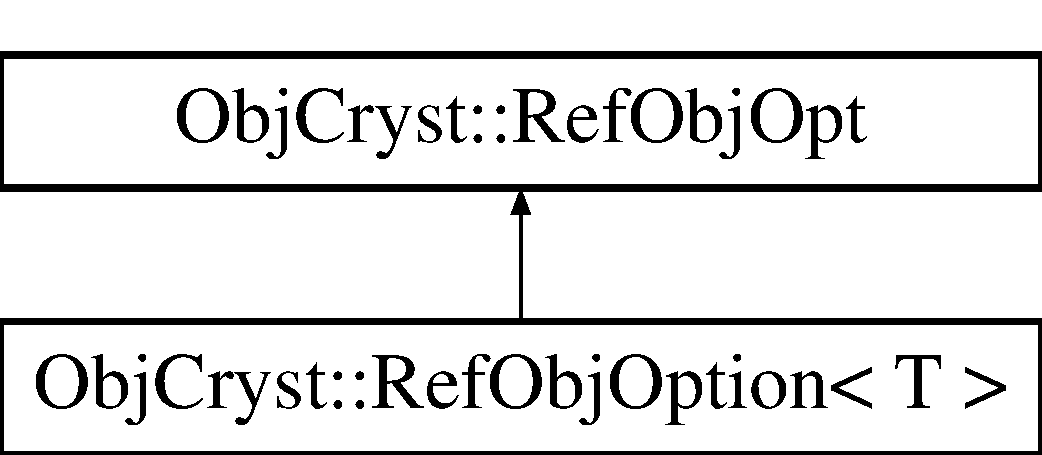
\includegraphics[height=2.000000cm]{a00078}
\end{center}
\end{figure}
\subsubsection*{\-Public \-Member \-Functions}
\begin{DoxyCompactItemize}
\item 
{\bf \-Ref\-Obj\-Opt} ()
\begin{DoxyCompactList}\small\item\em \-Constructor for the option. \end{DoxyCompactList}\item 
void {\bfseries \-Init} (const int nb\-Choice, const string $\ast$name, const string $\ast$choice\-Names)\label{a00078_acb2124833f426224863027d1f3f0e9d6}

\item 
int {\bfseries \-Get\-Nb\-Choice} () const \label{a00078_aeee7a18a06caf2e9de43f195c7ecee00}

\item 
int {\bfseries \-Get\-Choice} () const \label{a00078_a9c4ccafc994514e39266a1b6d91e1f42}

\item 
virtual void {\bfseries \-Set\-Choice} (const int choice)\label{a00078_a0333cbcd6ff10a2ee9aae0bafd3770c5}

\item 
void {\bfseries \-Set\-Choice} (const string \&choice\-Name)\label{a00078_a9a92c1a5543e46119687462a1b7e706e}

\item 
const string \& {\bfseries \-Get\-Name} () const \label{a00078_ab0bd1fc64b59914f2b8596f5537ecd67}

\item 
const string \& {\bfseries \-Get\-Class\-Name} () const \label{a00078_ad2d43141d9d301527bf134ff5c4f34f0}

\item 
const string \& {\bfseries \-Get\-Choice\-Name} (const int i) const \label{a00078_ae00a732dceaa596d2129805a44bcdddc}

\item 
const {\bf \-Refinable\-Obj\-Clock} \& {\bfseries \-Get\-Clock} () const \label{a00078_a6c019a9936024016dc5704f93c117424}

\item 
void {\bf \-X\-M\-L\-Output} (ostream \&os, int indent=0) const 
\begin{DoxyCompactList}\small\item\em \-X\-M\-L\-Output to stream in well-\/formed \-X\-M\-L. \end{DoxyCompactList}\item 
void {\bf \-X\-M\-L\-Input} (istream \&is, const {\bf \-X\-M\-L\-Cryst\-Tag} \&tag)
\begin{DoxyCompactList}\small\item\em \-X\-M\-L\-Input \-From stream. \end{DoxyCompactList}\end{DoxyCompactItemize}
\subsubsection*{\-Protected \-Attributes}
\begin{DoxyCompactItemize}
\item 
int {\bf m\-Nb\-Choice}\label{a00078_a54ae7b002c156671d5b2176a46cf95d5}

\begin{DoxyCompactList}\small\item\em \-Number of different choice possible for this option. \end{DoxyCompactList}\item 
int {\bf m\-Choice}\label{a00078_a34f40080b3adac88e5ab7e290dc951ae}

\begin{DoxyCompactList}\small\item\em \-Current value. \end{DoxyCompactList}\item 
const string $\ast$ {\bf mp\-Name}
\begin{DoxyCompactList}\small\item\em (short) \-Name for this option. \end{DoxyCompactList}\item 
const string $\ast$ {\bf mp\-Choice\-Name}
\begin{DoxyCompactList}\small\item\em \-Names corresponding to each possible value of this option (\-Human-\/understandable). \end{DoxyCompactList}\item 
{\bf \-Refinable\-Obj\-Clock} {\bf m\-Clock}\label{a00078_ace306a0100bbb1678c9b8683a009dc81}

\begin{DoxyCompactList}\small\item\em \-The clock associated to this option. \end{DoxyCompactList}\end{DoxyCompactItemize}


\subsubsection{\-Detailed \-Description}
\-Base class for options. 



\subsubsection{\-Constructor \& \-Destructor \-Documentation}
\index{\-Obj\-Cryst\-::\-Ref\-Obj\-Opt@{\-Obj\-Cryst\-::\-Ref\-Obj\-Opt}!\-Ref\-Obj\-Opt@{\-Ref\-Obj\-Opt}}
\index{\-Ref\-Obj\-Opt@{\-Ref\-Obj\-Opt}!ObjCryst::RefObjOpt@{\-Obj\-Cryst\-::\-Ref\-Obj\-Opt}}
\paragraph[{\-Ref\-Obj\-Opt}]{\setlength{\rightskip}{0pt plus 5cm}{\bf \-Obj\-Cryst\-::\-Ref\-Obj\-Opt\-::\-Ref\-Obj\-Opt} (
\begin{DoxyParamCaption}
{}
\end{DoxyParamCaption}
)}\label{a00078_ad4fd60241264e22179c9ab33fc58867f}


\-Constructor for the option. 


\begin{DoxyParams}{\-Parameters}
{\em obj,\-:} & the \\
\hline
\end{DoxyParams}


\subsubsection{\-Member \-Function \-Documentation}
\index{\-Obj\-Cryst\-::\-Ref\-Obj\-Opt@{\-Obj\-Cryst\-::\-Ref\-Obj\-Opt}!\-X\-M\-L\-Input@{\-X\-M\-L\-Input}}
\index{\-X\-M\-L\-Input@{\-X\-M\-L\-Input}!ObjCryst::RefObjOpt@{\-Obj\-Cryst\-::\-Ref\-Obj\-Opt}}
\paragraph[{\-X\-M\-L\-Input}]{\setlength{\rightskip}{0pt plus 5cm}void {\bf \-Obj\-Cryst\-::\-Ref\-Obj\-Opt\-::\-X\-M\-L\-Input} (
\begin{DoxyParamCaption}
\item[{istream \&}]{is, }
\item[{const {\bf \-X\-M\-L\-Cryst\-Tag} \&}]{tag}
\end{DoxyParamCaption}
)}\label{a00078_a9562e469ee61a710e535594fe58f0744}


\-X\-M\-L\-Input \-From stream. 

\index{\-Obj\-Cryst\-::\-Ref\-Obj\-Opt@{\-Obj\-Cryst\-::\-Ref\-Obj\-Opt}!\-X\-M\-L\-Output@{\-X\-M\-L\-Output}}
\index{\-X\-M\-L\-Output@{\-X\-M\-L\-Output}!ObjCryst::RefObjOpt@{\-Obj\-Cryst\-::\-Ref\-Obj\-Opt}}
\paragraph[{\-X\-M\-L\-Output}]{\setlength{\rightskip}{0pt plus 5cm}void {\bf \-Obj\-Cryst\-::\-Ref\-Obj\-Opt\-::\-X\-M\-L\-Output} (
\begin{DoxyParamCaption}
\item[{ostream \&}]{os, }
\item[{int}]{indent = {\ttfamily 0}}
\end{DoxyParamCaption}
) const}\label{a00078_a5758abdb2557b2b2a2621e015fd8ad75}


\-X\-M\-L\-Output to stream in well-\/formed \-X\-M\-L. 

\-In this function the name used is that of the \-Option. 

\subsubsection{\-Member \-Data \-Documentation}
\index{\-Obj\-Cryst\-::\-Ref\-Obj\-Opt@{\-Obj\-Cryst\-::\-Ref\-Obj\-Opt}!mp\-Choice\-Name@{mp\-Choice\-Name}}
\index{mp\-Choice\-Name@{mp\-Choice\-Name}!ObjCryst::RefObjOpt@{\-Obj\-Cryst\-::\-Ref\-Obj\-Opt}}
\paragraph[{mp\-Choice\-Name}]{\setlength{\rightskip}{0pt plus 5cm}const string$\ast$ {\bf \-Obj\-Cryst\-::\-Ref\-Obj\-Opt\-::mp\-Choice\-Name}\hspace{0.3cm}{\ttfamily  [protected]}}\label{a00078_abc47d0f345c4121b6492e754b30f4fef}


\-Names corresponding to each possible value of this option (\-Human-\/understandable). 

\-Should be statically stored in the class using the option. \index{\-Obj\-Cryst\-::\-Ref\-Obj\-Opt@{\-Obj\-Cryst\-::\-Ref\-Obj\-Opt}!mp\-Name@{mp\-Name}}
\index{mp\-Name@{mp\-Name}!ObjCryst::RefObjOpt@{\-Obj\-Cryst\-::\-Ref\-Obj\-Opt}}
\paragraph[{mp\-Name}]{\setlength{\rightskip}{0pt plus 5cm}const string$\ast$ {\bf \-Obj\-Cryst\-::\-Ref\-Obj\-Opt\-::mp\-Name}\hspace{0.3cm}{\ttfamily  [protected]}}\label{a00078_a45eb6eed7f6578f438433acddb2f1eb2}


(short) \-Name for this option. 

\-Should be statically stored in the class using the option 

\-The documentation for this class was generated from the following file\-:\begin{DoxyCompactItemize}
\item 
\-Refinable\-Obj.\-h\end{DoxyCompactItemize}

\subsection{Obj\-Cryst\-:\-:Refinable\-Par Class Reference}
\label{a00079}\index{Obj\-Cryst\-::\-Refinable\-Par@{Obj\-Cryst\-::\-Refinable\-Par}}


Generic class for parameters of refinable objects.  


Inheritance diagram for Obj\-Cryst\-:\-:Refinable\-Par\-:\begin{figure}[H]
\begin{center}
\leavevmode
\includegraphics[height=2.000000cm]{a00079}
\end{center}
\end{figure}
\subsubsection*{Public Member Functions}
\begin{DoxyCompactItemize}
\item 
void {\bf X\-M\-L\-Output} (ostream \&os, const string \&name, int indent=0) const 
\begin{DoxyCompactList}\small\item\em X\-M\-L\-Output to stream in well-\/formed X\-M\-L. \end{DoxyCompactList}\item 
void {\bf X\-M\-L\-Output} (ostream \&os, int indent=0) const 
\begin{DoxyCompactList}\small\item\em X\-M\-L\-Output to stream in well-\/formed X\-M\-L. \end{DoxyCompactList}\item 
void {\bf X\-M\-L\-Input} (istream \&is, const {\bf X\-M\-L\-Cryst\-Tag} \&tag)
\begin{DoxyCompactList}\small\item\em X\-M\-L\-Input From stream. \end{DoxyCompactList}\end{DoxyCompactItemize}
\begin{Indent}{\bf Destructor \& Constructors}\par
\begin{DoxyCompactItemize}
\item 
{\bf Refinable\-Par} ()\label{a00079_ae358698d7ab55d87df8af8781946f293}

\begin{DoxyCompactList}\small\item\em Default Constructor. \end{DoxyCompactList}\item 
{\bf Refinable\-Par} (const string \&name, R\-E\-A\-L $\ast$ref\-Par, const R\-E\-A\-L min, const R\-E\-A\-L max, const {\bf Ref\-Par\-Type} $\ast$type, {\bf Ref\-Par\-Deriv\-Step\-Model} deriv\-Mode=R\-E\-F\-P\-A\-R\-\_\-\-D\-E\-R\-I\-V\-\_\-\-S\-T\-E\-P\-\_\-\-R\-E\-L\-A\-T\-I\-V\-E, const bool has\-Limits=true, const bool is\-Fixed=false, const bool is\-Used=true, const bool is\-Periodic=false, const R\-E\-A\-L human\-Scale=1., R\-E\-A\-L period=1.)
\begin{DoxyCompactList}\small\item\em Constructor. \end{DoxyCompactList}\item 
{\bf Refinable\-Par} (const {\bf Refinable\-Par} \&ref)\label{a00079_a99cdc4550c46d90daf63b7f2e6d8d3c3}

\begin{DoxyCompactList}\small\item\em Copy Constructor. \end{DoxyCompactList}\item 
{\bfseries $\sim$\-Refinable\-Par} ()\label{a00079_ada37c0119416edb03732703afaf737a1}

\item 
void {\bf Init} (const string \&name, R\-E\-A\-L $\ast$ref\-Par, const R\-E\-A\-L min, const R\-E\-A\-L max, const {\bf Ref\-Par\-Type} $\ast$type, {\bf Ref\-Par\-Deriv\-Step\-Model} deriv\-Mode=R\-E\-F\-P\-A\-R\-\_\-\-D\-E\-R\-I\-V\-\_\-\-S\-T\-E\-P\-\_\-\-R\-E\-L\-A\-T\-I\-V\-E, const bool has\-Limits=true, const bool is\-Fixed=false, const bool is\-Used=true, const bool is\-Periodic=false, const R\-E\-A\-L human\-Scale=1., R\-E\-A\-L period=1.)
\begin{DoxyCompactList}\small\item\em Constructor. \end{DoxyCompactList}\item 
void {\bf Copy\-Attributes} (const {\bf Refinable\-Par} \&)
\begin{DoxyCompactList}\small\item\em Copy all attributes (limits, flags, etc...) from another \doxyref{Refinable\-Par}{p.}{a00079} object. \end{DoxyCompactList}\end{DoxyCompactItemize}
\end{Indent}
\begin{Indent}{\bf Access \& change the current value of the parameter}\par
\begin{DoxyCompactItemize}
\item 
R\-E\-A\-L {\bf Get\-Value} () const 
\begin{DoxyCompactList}\small\item\em of the parameter. \end{DoxyCompactList}\item 
const R\-E\-A\-L $\ast$ {\bf Get\-Pointer} () const 
\begin{DoxyCompactList}\small\item\em Access to a const pointer to the refined value. \end{DoxyCompactList}\item 
void {\bf Set\-Value} (const R\-E\-A\-L value)
\begin{DoxyCompactList}\small\item\em of the parameter. \end{DoxyCompactList}\item 
const R\-E\-A\-L \& {\bf Get\-Human\-Value} () const \label{a00079_ae1ffe41bcce38c1dc9bf0d649fc06adc}

\begin{DoxyCompactList}\small\item\em Current value of parameter, scaled if necessary (for angles) to a human-\/understandable value. \end{DoxyCompactList}\item 
void {\bf Set\-Human\-Value} (const R\-E\-A\-L \&)\label{a00079_a6bb727ce1de6de9e56c46be1ba75f8b9}

\begin{DoxyCompactList}\small\item\em Current value of parameter, scaled if necessary (for angles) to a human-\/understandable value. \end{DoxyCompactList}\item 
void {\bf Mutate} (const R\-E\-A\-L mutate\-Value)
\begin{DoxyCompactList}\small\item\em Add the given amount to the parameter current value. \end{DoxyCompactList}\item 
void {\bf Mutate\-To} (const R\-E\-A\-L new\-Value)
\begin{DoxyCompactList}\small\item\em Change the current value to the given one. \end{DoxyCompactList}\item 
R\-E\-A\-L {\bfseries Get\-Sigma} () const \label{a00079_aa47f29ee29133f35d3217cfd68b02d57}

\item 
R\-E\-A\-L {\bfseries Get\-Human\-Sigma} () const \label{a00079_a932c8eeab6494b0d67984736560b5b46}

\item 
void {\bfseries Set\-Sigma} (const R\-E\-A\-L)\label{a00079_af199d90bd14333483929aab3a898ae39}

\end{DoxyCompactItemize}
\end{Indent}
\begin{Indent}{\bf General info}\par
\begin{DoxyCompactItemize}
\item 
string {\bf Get\-Name} () const \label{a00079_a0daa7c9ec87518347736e4fa6e45a333}

\begin{DoxyCompactList}\small\item\em Get the parameter's name. \end{DoxyCompactList}\item 
void {\bf Set\-Name} (const string \&)\label{a00079_ac8e91083b8d0c3fe1d3f349122756abb}

\begin{DoxyCompactList}\small\item\em Set the name of the parameter. It should be unique in the \doxyref{Refinable\-Obj}{p.}{a00077}. \end{DoxyCompactList}\item 
void {\bfseries Print} () const \label{a00079_a829f3712a893e3284dfc461d6e7bf016}

\item 
bool {\bfseries Is\-Fixed} () const \label{a00079_a11f0f58b66d069ae9353cd944a0b90ee}

\item 
void {\bfseries Set\-Is\-Fixed} (const bool)\label{a00079_a57690ad69493beb8f2b8976c10833640}

\item 
bool {\bfseries Is\-Limited} () const \label{a00079_ab2421bf2583d6583bc1cf0e1a65ce574}

\item 
void {\bfseries Set\-Is\-Limited} (const bool)\label{a00079_a90c20ed99e6782b6a5abc6d5a6abb105}

\item 
bool {\bf Is\-Used} () const \label{a00079_aa71a1c66f87d910c352286e2ef51c9c9}

\begin{DoxyCompactList}\small\item\em Is the parameter used (if not, it is simply irrelevant in the model) ? \end{DoxyCompactList}\item 
void {\bf Set\-Is\-Used} (const bool)\label{a00079_aea29e6822f1a6215c274cacf5c58e7ce}

\begin{DoxyCompactList}\small\item\em Is the parameter used (if not, it is simply irrelevant in the model) ? \end{DoxyCompactList}\item 
bool {\bfseries Is\-Periodic} () const \label{a00079_a886b2db23080365ef90870e846a27dfa}

\item 
void {\bfseries Set\-Is\-Periodic} (const bool, R\-E\-A\-L period=1)\label{a00079_a3e131a39649e853afb121ce5c9b5ebe1}

\item 
R\-E\-A\-L {\bf Get\-Human\-Scale} () const \label{a00079_a97fb48bd2b4d6845d5543573dad84aea}

\begin{DoxyCompactList}\small\item\em Human scale for this parameter \-: for angles, this is equal to 180/pi. \end{DoxyCompactList}\item 
void {\bf Set\-Human\-Scale} (const R\-E\-A\-L)\label{a00079_a05a23549ca32b4745dee0a1bb539830e}

\begin{DoxyCompactList}\small\item\em Human scale for this parameter \-: for angles, this is equal to 180/pi. \end{DoxyCompactList}\end{DoxyCompactItemize}
\end{Indent}
\begin{Indent}{\bf Min, max values}\par
\begin{DoxyCompactItemize}
\item 
R\-E\-A\-L {\bf Get\-Min} () const \label{a00079_a27d046a98b774ff373aec8a6aeca31ae}

\begin{DoxyCompactList}\small\item\em Minimum value allowed (if limited or periodic) \end{DoxyCompactList}\item 
void {\bf Set\-Min} (const R\-E\-A\-L)\label{a00079_a82ece8fe469cfc3582f7d5d899928630}

\begin{DoxyCompactList}\small\item\em Set the Minimum value allowed (if limited) \end{DoxyCompactList}\item 
R\-E\-A\-L {\bf Get\-Human\-Min} () const \label{a00079_a8f9a61e06332dd459ed55c117b9c7475}

\begin{DoxyCompactList}\small\item\em Get the minimum value allowed (if limited) \end{DoxyCompactList}\item 
void {\bf Set\-Human\-Min} (const R\-E\-A\-L)\label{a00079_ad4ba7c4c6d1c46c9334dcc0673df4fb2}

\begin{DoxyCompactList}\small\item\em Set the minimum value allowed (if limited) \end{DoxyCompactList}\item 
R\-E\-A\-L {\bf Get\-Max} () const \label{a00079_ab1e49d10dd00c3ba156d2adb9d0dc6b3}

\begin{DoxyCompactList}\small\item\em Get the maximum value allowed (if limited) \end{DoxyCompactList}\item 
void {\bf Set\-Max} (const R\-E\-A\-L)\label{a00079_a33f45d527d405da957ddc513e5a3099f}

\begin{DoxyCompactList}\small\item\em Get the maximum value allowed (if limited) \end{DoxyCompactList}\item 
R\-E\-A\-L {\bf Get\-Human\-Max} () const \label{a00079_ad4a7468d788806cd893fcca83534eb83}

\begin{DoxyCompactList}\small\item\em Get the maximum value allowed (if limited) \end{DoxyCompactList}\item 
void {\bf Set\-Human\-Max} (const R\-E\-A\-L)\label{a00079_ade6c83881319be43feb679b4896766bd}

\begin{DoxyCompactList}\small\item\em Get the maximum value allowed (if limited) \end{DoxyCompactList}\item 
R\-E\-A\-L {\bf Get\-Period} () const \label{a00079_a2bc0ba973f3e0e5eb93be0a0ebc29c93}

\begin{DoxyCompactList}\small\item\em Get the period (if periodic) \end{DoxyCompactList}\item 
void {\bf Set\-Period} (const R\-E\-A\-L)\label{a00079_a97b23ea6b624bbe517c29b5ef00b5f5b}

\begin{DoxyCompactList}\small\item\em Set the period value (if periodic) \end{DoxyCompactList}\end{DoxyCompactItemize}
\end{Indent}
\begin{Indent}{\bf Steps during refinement}\par
\begin{DoxyCompactItemize}
\item 
R\-E\-A\-L {\bf Get\-Deriv\-Step} () const \label{a00079_a8ba4cbee715d51c85ce5147ce9cf45db}

\begin{DoxyCompactList}\small\item\em Fixed step to use to compute numerical derivative. \end{DoxyCompactList}\item 
void {\bf Set\-Deriv\-Step} (const R\-E\-A\-L)\label{a00079_a3156b809e45a6314a680bbe3dec1a573}

\begin{DoxyCompactList}\small\item\em Fixed step to use to compute numerical derivative. \end{DoxyCompactList}\item 
R\-E\-A\-L {\bf Get\-Global\-Optim\-Step} () const \label{a00079_a2fb1982abc56de79e7dd79ee6bbd0e3f}

\begin{DoxyCompactList}\small\item\em Maximum step to use during Global Optimization algorithms. \end{DoxyCompactList}\item 
void {\bf Set\-Global\-Optim\-Step} (const R\-E\-A\-L)\label{a00079_aa0eccaf87210097fb9e5239a97f9dcd1}

\begin{DoxyCompactList}\small\item\em Maximum step to use during Global Optimization algorithms. \end{DoxyCompactList}\end{DoxyCompactItemize}
\end{Indent}
\begin{Indent}{\bf Parameter's Clock}\par
\begin{DoxyCompactItemize}
\item 
void {\bf Assign\-Clock} ({\bf Refinable\-Obj\-Clock} \&clock)
\item 
const {\bf Refinable\-Obj\-Clock} \& {\bf Get\-Clock} () const \label{a00079_a18c0d07d6795a1016af3bda5cca694a2}

\begin{DoxyCompactList}\small\item\em Get a constant reference to the clock assigned to this parameter. \end{DoxyCompactList}\item 
{\bf Refinable\-Obj\-Clock} \& {\bf Get\-Clock} ()\label{a00079_ad6495758297cf923c8746cb3734fc838}

\begin{DoxyCompactList}\small\item\em Get a reference to the clock assigned to this parameter. \end{DoxyCompactList}\end{DoxyCompactItemize}
\end{Indent}
\begin{Indent}{\bf Change Limits}\par
\begin{DoxyCompactItemize}
\item 
void {\bf Set\-Limits\-Absolute} (const R\-E\-A\-L min, const R\-E\-A\-L max)\label{a00079_aad4275aa946de7b60aaf3353971663dd}

\begin{DoxyCompactList}\small\item\em Change the limits for this object, giving absolute new limits. \end{DoxyCompactList}\item 
void {\bf Set\-Limits\-Relative} (const R\-E\-A\-L min, const R\-E\-A\-L max)
\begin{DoxyCompactList}\small\item\em Change the limits for this object, giving relative new limits (eg giving -\/.\-1 and +.1 will set new limits at the current value + min and current value + max) Thus min should logically be $<$0 and max $>$0. \end{DoxyCompactList}\item 
void {\bf Set\-Limits\-Proportional} (const R\-E\-A\-L min, const R\-E\-A\-L max)
\begin{DoxyCompactList}\small\item\em Change the limits for this object, proportionnaly to the current value. \end{DoxyCompactList}\end{DoxyCompactItemize}
\end{Indent}
\subsubsection*{Private Member Functions}
\begin{DoxyCompactItemize}
\item 
void {\bf Click} ()\label{a00079_a3dc5a8cf7fb9d3c800fe6dd494054d92}

\begin{DoxyCompactList}\small\item\em Click the Clock ! to telle the \doxyref{Refinable\-Obj}{p.}{a00077} it has been modified. \end{DoxyCompactList}\end{DoxyCompactItemize}
\subsubsection*{Private Attributes}
\begin{DoxyCompactItemize}
\item 
string {\bf m\-Name}\label{a00079_afe5091b81dec1c77b7ec98f473f40698}

\begin{DoxyCompactList}\small\item\em name of the refinable parameter \end{DoxyCompactList}\item 
R\-E\-A\-L $\ast$ {\bf mp\-Value}\label{a00079_a8bfbe4ae25c98850480c70a2cde259dc}

\begin{DoxyCompactList}\small\item\em Pointer to the refinable value. \end{DoxyCompactList}\item 
R\-E\-A\-L {\bf m\-Min}\label{a00079_a303f811dfa1a8592ed2a72c489eabe1e}

\begin{DoxyCompactList}\small\item\em Hard lower and upper limits. \end{DoxyCompactList}\item 
R\-E\-A\-L {\bfseries m\-Max}\label{a00079_ae16a4a1d93b0f86e683f2a51ab4d627f}

\item 
bool {\bf m\-Has\-Limits}\label{a00079_a867316e66708e8d7efb64b9064f5241a}

\begin{DoxyCompactList}\small\item\em Does the refinable parameter need limits (min and max) ? \end{DoxyCompactList}\item 
bool {\bf m\-Is\-Fixed}\label{a00079_acf1638fe7459af0df2f64279115f6091}

\begin{DoxyCompactList}\small\item\em is the parameter currently fixed ? \end{DoxyCompactList}\item 
bool {\bf m\-Is\-Used}\label{a00079_a9d6d609d62226ba7c6fe1a1fd694b77d}

\begin{DoxyCompactList}\small\item\em Is the parameter currently used ? \end{DoxyCompactList}\item 
bool {\bf m\-Is\-Periodic}
\begin{DoxyCompactList}\small\item\em Is the parameter periodic ? If this is the case, then when using the \doxyref{Refinable\-Par\-::\-Mutate()}{p.}{a00079_abd6a06bbb5eb59d80515ebdad2612da8} function, if the parameter goes beyond its limits, it will be shifted by the value of its period. \end{DoxyCompactList}\item 
R\-E\-A\-L {\bf m\-Period}\label{a00079_ae33430ff688a0a5e4e907ab8bbee0ecd}

\begin{DoxyCompactList}\small\item\em Period value (if relevant) \end{DoxyCompactList}\item 
R\-E\-A\-L {\bf m\-Global\-Optim\-Step}\label{a00079_a3d5465cf22c3080f856825c29f45e201}

\begin{DoxyCompactList}\small\item\em Step to use for global method search (simulated annealing,...) \end{DoxyCompactList}\item 
R\-E\-A\-L {\bf m\-Deriv\-Step}\label{a00079_a07c0acd9afc24e5945bfa8a9e940002d}

\begin{DoxyCompactList}\small\item\em Step to use for numerical derivative calculation. \end{DoxyCompactList}\item 
{\bf Ref\-Par\-Deriv\-Step\-Model} {\bf m\-Ref\-Par\-Deriv\-Step\-Model}\label{a00079_adb6f88fa2781510eef3e024accda52ed}

\begin{DoxyCompactList}\small\item\em Model followed for derivation. \end{DoxyCompactList}\item 
R\-E\-A\-L {\bf m\-Sigma}\label{a00079_a943363b2a00d01575668ad6d3e27dafb}

\begin{DoxyCompactList}\small\item\em Calculated sigma on value. \end{DoxyCompactList}\item 
R\-E\-A\-L {\bf m\-Human\-Scale}
\begin{DoxyCompactList}\small\item\em Scale to be used to display 'human' value. \end{DoxyCompactList}\item 
bool {\bf m\-Has\-Assigned\-Clock}\label{a00079_a32ec16db6ad86efc4bd14dcfbb0e9712}

\begin{DoxyCompactList}\small\item\em Is there a clock associated with this parameter ? If yes, then it must \doxyref{Click()}{p.}{a00079_a3dc5a8cf7fb9d3c800fe6dd494054d92} it each time it is modified. \end{DoxyCompactList}\item 
{\bf Refinable\-Obj\-Clock} $\ast$ {\bfseries mp\-Clock}\label{a00079_a3c6145e3df75637040f0b2e64ec00382}

\end{DoxyCompactItemize}
\subsubsection*{Friends}
\begin{DoxyCompactItemize}
\item 
class {\bfseries Refinable\-Obj}\label{a00079_a4b004207cfa15cef5b32be20104e3eaf}

\end{DoxyCompactItemize}


\subsubsection{Detailed Description}
Generic class for parameters of refinable objects. 

These must be continuous.

\begin{DoxyRefDesc}{Todo}
\item[{\bf Todo}]\-: define parameters using equations between parameters. 

\-: for complex objects with lots of parameters, give the possibility to define vectors of parameters, all with the same properties, to reduce memory usage. \end{DoxyRefDesc}


\subsubsection{Constructor \& Destructor Documentation}
\index{Obj\-Cryst\-::\-Refinable\-Par@{Obj\-Cryst\-::\-Refinable\-Par}!Refinable\-Par@{Refinable\-Par}}
\index{Refinable\-Par@{Refinable\-Par}!ObjCryst::RefinablePar@{Obj\-Cryst\-::\-Refinable\-Par}}
\paragraph[{Refinable\-Par}]{\setlength{\rightskip}{0pt plus 5cm}Obj\-Cryst\-::\-Refinable\-Par\-::\-Refinable\-Par (
\begin{DoxyParamCaption}
\item[{const string \&}]{name, }
\item[{R\-E\-A\-L $\ast$}]{ref\-Par, }
\item[{const R\-E\-A\-L}]{min, }
\item[{const R\-E\-A\-L}]{max, }
\item[{const {\bf Ref\-Par\-Type} $\ast$}]{type, }
\item[{{\bf Ref\-Par\-Deriv\-Step\-Model}}]{deriv\-Mode = {\ttfamily REFPAR\-\_\-DERIV\-\_\-STEP\-\_\-RELATIVE}, }
\item[{const bool}]{has\-Limits = {\ttfamily true}, }
\item[{const bool}]{is\-Fixed = {\ttfamily false}, }
\item[{const bool}]{is\-Used = {\ttfamily true}, }
\item[{const bool}]{is\-Periodic = {\ttfamily false}, }
\item[{const R\-E\-A\-L}]{human\-Scale = {\ttfamily 1.}, }
\item[{R\-E\-A\-L}]{period = {\ttfamily 1.}}
\end{DoxyParamCaption}
)}\label{a00079_ac82759679653390c868ca7cbcb7e572c}


Constructor. 

\begin{DoxyParagraph}{name\-: the name of the parameter}

\end{DoxyParagraph}
\begin{DoxyParagraph}{ref\-Par\-: the address of the refined parameter}

\end{DoxyParagraph}
\begin{DoxyParagraph}{min,max\-: the minimum \& maximum value for this parameter. Only used}
if the parameter is limited. 
\end{DoxyParagraph}
\begin{DoxyParagraph}{type\-: the type (category) of refinable parameter. This is used to (de)activate}
groups of parameters. 
\end{DoxyParagraph}
\begin{DoxyParagraph}{deriv\-Mode\-: to compute numerical (partial) derivatives, the step used is either}
an absolute (fixed) value, or it can be proportionnal to the current value of the parameter. 
\end{DoxyParagraph}
\begin{DoxyParagraph}{has\-Limits\-: if true, then the parameter cannot exceed its limits.}

\end{DoxyParagraph}
\begin{DoxyParagraph}{is\-Fixed\-: if true, the parameter cannot be refined.}

\end{DoxyParagraph}
\begin{DoxyParagraph}{is\-Used\-: if false, then the parameter does not affect in any way the refined object,}
and thus is simply ignored and should never appear to the user. 
\end{DoxyParagraph}
\begin{DoxyParagraph}{is\-Periodic\-: if true, then when the parameter exceeds one of its limits, it is}
shifted by the period (=max-\/min), in order to be back to the allowed [min,max] range. 
\end{DoxyParagraph}
\begin{DoxyParagraph}{human\-Scale\-:this is the scale which should be used to display the value to the}
end program user. This is mostly used for angles\-: the values are stored in radians, so that a scale equal to 180/pi must be used for a 'human-\/understandable' value. Use the Refinable\-Par\-::\-Human\-Value() in order to get this value. By default it is equal to 1.\-0 (no scaling required). 
\end{DoxyParagraph}


\subsubsection{Member Function Documentation}
\index{Obj\-Cryst\-::\-Refinable\-Par@{Obj\-Cryst\-::\-Refinable\-Par}!Assign\-Clock@{Assign\-Clock}}
\index{Assign\-Clock@{Assign\-Clock}!ObjCryst::RefinablePar@{Obj\-Cryst\-::\-Refinable\-Par}}
\paragraph[{Assign\-Clock}]{\setlength{\rightskip}{0pt plus 5cm}void Obj\-Cryst\-::\-Refinable\-Par\-::\-Assign\-Clock (
\begin{DoxyParamCaption}
\item[{{\bf Refinable\-Obj\-Clock} \&}]{clock}
\end{DoxyParamCaption}
)}\label{a00079_ab03f6bffb78dd812136a73b94b64ee6e}
Assign a clock to this parameter. Any time this parameter is modified, the clock will be ticked ! \index{Obj\-Cryst\-::\-Refinable\-Par@{Obj\-Cryst\-::\-Refinable\-Par}!Copy\-Attributes@{Copy\-Attributes}}
\index{Copy\-Attributes@{Copy\-Attributes}!ObjCryst::RefinablePar@{Obj\-Cryst\-::\-Refinable\-Par}}
\paragraph[{Copy\-Attributes}]{\setlength{\rightskip}{0pt plus 5cm}void Obj\-Cryst\-::\-Refinable\-Par\-::\-Copy\-Attributes (
\begin{DoxyParamCaption}
\item[{const {\bf Refinable\-Par} \&}]{}
\end{DoxyParamCaption}
)}\label{a00079_a5882aec9561125f6e81b81f175031652}


Copy all attributes (limits, flags, etc...) from another \doxyref{Refinable\-Par}{p.}{a00079} object. 

This is useful in \doxyref{Refinable\-Obj}{p.}{a00077} copy constructors. Everything is copied but the pointer to the value refined, and the pointer to the clock. \index{Obj\-Cryst\-::\-Refinable\-Par@{Obj\-Cryst\-::\-Refinable\-Par}!Get\-Pointer@{Get\-Pointer}}
\index{Get\-Pointer@{Get\-Pointer}!ObjCryst::RefinablePar@{Obj\-Cryst\-::\-Refinable\-Par}}
\paragraph[{Get\-Pointer}]{\setlength{\rightskip}{0pt plus 5cm}const R\-E\-A\-L$\ast$ Obj\-Cryst\-::\-Refinable\-Par\-::\-Get\-Pointer (
\begin{DoxyParamCaption}
{}
\end{DoxyParamCaption}
) const}\label{a00079_a128e04b0731ed791ecc3afc228d6f17e}


Access to a const pointer to the refined value. 

This can be used to identify the parameter \index{Obj\-Cryst\-::\-Refinable\-Par@{Obj\-Cryst\-::\-Refinable\-Par}!Get\-Value@{Get\-Value}}
\index{Get\-Value@{Get\-Value}!ObjCryst::RefinablePar@{Obj\-Cryst\-::\-Refinable\-Par}}
\paragraph[{Get\-Value}]{\setlength{\rightskip}{0pt plus 5cm}R\-E\-A\-L Obj\-Cryst\-::\-Refinable\-Par\-::\-Get\-Value (
\begin{DoxyParamCaption}
{}
\end{DoxyParamCaption}
) const}\label{a00079_ad27e4b5ed56bdf316c8d322537a7c85a}


of the parameter. 

Use the The \doxyref{Mutate()}{p.}{a00079_abd6a06bbb5eb59d80515ebdad2612da8} and \doxyref{Mutate\-To()}{p.}{a00079_a696f87a0a129cfd270144532d664d093} function to change this value. \index{Obj\-Cryst\-::\-Refinable\-Par@{Obj\-Cryst\-::\-Refinable\-Par}!Init@{Init}}
\index{Init@{Init}!ObjCryst::RefinablePar@{Obj\-Cryst\-::\-Refinable\-Par}}
\paragraph[{Init}]{\setlength{\rightskip}{0pt plus 5cm}void Obj\-Cryst\-::\-Refinable\-Par\-::\-Init (
\begin{DoxyParamCaption}
\item[{const string \&}]{name, }
\item[{R\-E\-A\-L $\ast$}]{ref\-Par, }
\item[{const R\-E\-A\-L}]{min, }
\item[{const R\-E\-A\-L}]{max, }
\item[{const {\bf Ref\-Par\-Type} $\ast$}]{type, }
\item[{{\bf Ref\-Par\-Deriv\-Step\-Model}}]{deriv\-Mode = {\ttfamily REFPAR\-\_\-DERIV\-\_\-STEP\-\_\-RELATIVE}, }
\item[{const bool}]{has\-Limits = {\ttfamily true}, }
\item[{const bool}]{is\-Fixed = {\ttfamily false}, }
\item[{const bool}]{is\-Used = {\ttfamily true}, }
\item[{const bool}]{is\-Periodic = {\ttfamily false}, }
\item[{const R\-E\-A\-L}]{human\-Scale = {\ttfamily 1.}, }
\item[{R\-E\-A\-L}]{period = {\ttfamily 1.}}
\end{DoxyParamCaption}
)}\label{a00079_a58cbd1b3c3ada8383ddb444f879a9495}


Constructor. 

\begin{DoxyParagraph}{name\-: the name of the parameter}

\end{DoxyParagraph}
\begin{DoxyParagraph}{ref\-Par\-: the address of the refined parameter}

\end{DoxyParagraph}
\begin{DoxyParagraph}{min,max\-: the minimum \& maximum value for this parameter. Only used}
if the parameter is limited. 
\end{DoxyParagraph}
\begin{DoxyParagraph}{type\-: the type (category) of refinable parameter. This is used to (de)activate}
groups of parameters. 
\end{DoxyParagraph}
\begin{DoxyParagraph}{deriv\-Mode\-: to compute numerical (partial) derivatives, the step used is either}
an absolute (fixed) value, or it can be proportionnal to the current value of the parameter. 
\end{DoxyParagraph}
\begin{DoxyParagraph}{has\-Limits\-: if true, then the parameter cannot exceed its limits.}

\end{DoxyParagraph}
\begin{DoxyParagraph}{is\-Fixed\-: if true, the parameter cannot be refined.}

\end{DoxyParagraph}
\begin{DoxyParagraph}{is\-Used\-: if false, then the parameter does not affect in any way the refined object,}
and thus is simply ignored and should never appear to the user. 
\end{DoxyParagraph}
\begin{DoxyParagraph}{is\-Periodic\-: if true, then when the parameter exceeds one of its limits, it is}
shifted by the period (=max-\/min), in order to be back to the allowed [min,max] range. 
\end{DoxyParagraph}
\begin{DoxyParagraph}{human\-Scale\-:this is the scale which should be used to display the value to the}
end program user. This is mostly used for angles\-: the values are stored in radians, so that a scale equal to 180/pi must be used for a 'human-\/understandable' value. Use the Refinable\-Par\-::\-Human\-Value() in order to get this value. By default it is equal to 1.\-0 (no scaling required). 
\end{DoxyParagraph}
\index{Obj\-Cryst\-::\-Refinable\-Par@{Obj\-Cryst\-::\-Refinable\-Par}!Mutate@{Mutate}}
\index{Mutate@{Mutate}!ObjCryst::RefinablePar@{Obj\-Cryst\-::\-Refinable\-Par}}
\paragraph[{Mutate}]{\setlength{\rightskip}{0pt plus 5cm}void Obj\-Cryst\-::\-Refinable\-Par\-::\-Mutate (
\begin{DoxyParamCaption}
\item[{const R\-E\-A\-L}]{mutate\-Value}
\end{DoxyParamCaption}
)}\label{a00079_abd6a06bbb5eb59d80515ebdad2612da8}


Add the given amount to the parameter current value. 

If limit is hit, set to limit. If the limit is hit {\itshape and} the parameter is periodic, shift by period to bring back to allowed values. \begin{DoxyWarning}{Warning}
Will throw an exception if the parameter is defined by an equation. 
\end{DoxyWarning}
\index{Obj\-Cryst\-::\-Refinable\-Par@{Obj\-Cryst\-::\-Refinable\-Par}!Mutate\-To@{Mutate\-To}}
\index{Mutate\-To@{Mutate\-To}!ObjCryst::RefinablePar@{Obj\-Cryst\-::\-Refinable\-Par}}
\paragraph[{Mutate\-To}]{\setlength{\rightskip}{0pt plus 5cm}void Obj\-Cryst\-::\-Refinable\-Par\-::\-Mutate\-To (
\begin{DoxyParamCaption}
\item[{const R\-E\-A\-L}]{new\-Value}
\end{DoxyParamCaption}
)}\label{a00079_a696f87a0a129cfd270144532d664d093}


Change the current value to the given one. 

If the limit is hit, then set to the limit (unless the pameter is periodic, then shift by the period amount back to allowed values). \begin{DoxyWarning}{Warning}
Will throw an exception if the parameter is defined by an equation. 
\end{DoxyWarning}
\index{Obj\-Cryst\-::\-Refinable\-Par@{Obj\-Cryst\-::\-Refinable\-Par}!Set\-Limits\-Proportional@{Set\-Limits\-Proportional}}
\index{Set\-Limits\-Proportional@{Set\-Limits\-Proportional}!ObjCryst::RefinablePar@{Obj\-Cryst\-::\-Refinable\-Par}}
\paragraph[{Set\-Limits\-Proportional}]{\setlength{\rightskip}{0pt plus 5cm}void Obj\-Cryst\-::\-Refinable\-Par\-::\-Set\-Limits\-Proportional (
\begin{DoxyParamCaption}
\item[{const R\-E\-A\-L}]{min, }
\item[{const R\-E\-A\-L}]{max}
\end{DoxyParamCaption}
)}\label{a00079_afb15606bb24a5fbb144d07843bb11f97}


Change the limits for this object, proportionnaly to the current value. 

min should be $<$ 1. and max $>$ 1. \index{Obj\-Cryst\-::\-Refinable\-Par@{Obj\-Cryst\-::\-Refinable\-Par}!Set\-Limits\-Relative@{Set\-Limits\-Relative}}
\index{Set\-Limits\-Relative@{Set\-Limits\-Relative}!ObjCryst::RefinablePar@{Obj\-Cryst\-::\-Refinable\-Par}}
\paragraph[{Set\-Limits\-Relative}]{\setlength{\rightskip}{0pt plus 5cm}void Obj\-Cryst\-::\-Refinable\-Par\-::\-Set\-Limits\-Relative (
\begin{DoxyParamCaption}
\item[{const R\-E\-A\-L}]{min, }
\item[{const R\-E\-A\-L}]{max}
\end{DoxyParamCaption}
)}\label{a00079_ad445354c927f8df95443a55174e7bb7d}


Change the limits for this object, giving relative new limits (eg giving -\/.\-1 and +.1 will set new limits at the current value + min and current value + max) Thus min should logically be $<$0 and max $>$0. 

\index{Obj\-Cryst\-::\-Refinable\-Par@{Obj\-Cryst\-::\-Refinable\-Par}!Set\-Value@{Set\-Value}}
\index{Set\-Value@{Set\-Value}!ObjCryst::RefinablePar@{Obj\-Cryst\-::\-Refinable\-Par}}
\paragraph[{Set\-Value}]{\setlength{\rightskip}{0pt plus 5cm}void Obj\-Cryst\-::\-Refinable\-Par\-::\-Set\-Value (
\begin{DoxyParamCaption}
\item[{const R\-E\-A\-L}]{value}
\end{DoxyParamCaption}
)}\label{a00079_a55a87d842fc046b2f4b3c03c92e53052}


of the parameter. 

Use the The \doxyref{Mutate()}{p.}{a00079_abd6a06bbb5eb59d80515ebdad2612da8} and \doxyref{Mutate\-To()}{p.}{a00079_a696f87a0a129cfd270144532d664d093} function to change this value. \index{Obj\-Cryst\-::\-Refinable\-Par@{Obj\-Cryst\-::\-Refinable\-Par}!X\-M\-L\-Input@{X\-M\-L\-Input}}
\index{X\-M\-L\-Input@{X\-M\-L\-Input}!ObjCryst::RefinablePar@{Obj\-Cryst\-::\-Refinable\-Par}}
\paragraph[{X\-M\-L\-Input}]{\setlength{\rightskip}{0pt plus 5cm}void Obj\-Cryst\-::\-Refinable\-Par\-::\-X\-M\-L\-Input (
\begin{DoxyParamCaption}
\item[{istream \&}]{is, }
\item[{const {\bf X\-M\-L\-Cryst\-Tag} \&}]{tag}
\end{DoxyParamCaption}
)}\label{a00079_af6fcabe9e97e0aabacef7a9bee5d1106}


X\-M\-L\-Input From stream. 

\index{Obj\-Cryst\-::\-Refinable\-Par@{Obj\-Cryst\-::\-Refinable\-Par}!X\-M\-L\-Output@{X\-M\-L\-Output}}
\index{X\-M\-L\-Output@{X\-M\-L\-Output}!ObjCryst::RefinablePar@{Obj\-Cryst\-::\-Refinable\-Par}}
\paragraph[{X\-M\-L\-Output}]{\setlength{\rightskip}{0pt plus 5cm}void Obj\-Cryst\-::\-Refinable\-Par\-::\-X\-M\-L\-Output (
\begin{DoxyParamCaption}
\item[{ostream \&}]{os, }
\item[{const string \&}]{name, }
\item[{int}]{indent = {\ttfamily 0}}
\end{DoxyParamCaption}
) const}\label{a00079_ae8271536206b603c717c5fa793b2310c}


X\-M\-L\-Output to stream in well-\/formed X\-M\-L. 

this will save the fixed \& limited flags, as well as limits 
\begin{DoxyParams}{Parameters}
{\em name} & the name to use instead of the Ref\-Par name. \\
\hline
\end{DoxyParams}
\index{Obj\-Cryst\-::\-Refinable\-Par@{Obj\-Cryst\-::\-Refinable\-Par}!X\-M\-L\-Output@{X\-M\-L\-Output}}
\index{X\-M\-L\-Output@{X\-M\-L\-Output}!ObjCryst::RefinablePar@{Obj\-Cryst\-::\-Refinable\-Par}}
\paragraph[{X\-M\-L\-Output}]{\setlength{\rightskip}{0pt plus 5cm}void Obj\-Cryst\-::\-Refinable\-Par\-::\-X\-M\-L\-Output (
\begin{DoxyParamCaption}
\item[{ostream \&}]{os, }
\item[{int}]{indent = {\ttfamily 0}}
\end{DoxyParamCaption}
) const}\label{a00079_a7105a845ac12a49b0a5fcb41a4e6cbde}


X\-M\-L\-Output to stream in well-\/formed X\-M\-L. 

this will save the fixed \& limited flags, as well as limits. In this function the name used is that of the Ref\-Par. 

\subsubsection{Member Data Documentation}
\index{Obj\-Cryst\-::\-Refinable\-Par@{Obj\-Cryst\-::\-Refinable\-Par}!m\-Human\-Scale@{m\-Human\-Scale}}
\index{m\-Human\-Scale@{m\-Human\-Scale}!ObjCryst::RefinablePar@{Obj\-Cryst\-::\-Refinable\-Par}}
\paragraph[{m\-Human\-Scale}]{\setlength{\rightskip}{0pt plus 5cm}R\-E\-A\-L Obj\-Cryst\-::\-Refinable\-Par\-::m\-Human\-Scale\hspace{0.3cm}{\ttfamily [private]}}\label{a00079_a1a0b4a89d0d106fe43d4ada7c44e4cd9}


Scale to be used to display 'human' value. 

This is for angular parameters\-: the computer stores values in radians, whil the user only understands degrees. So a scale factor of 180/pi is necessary. \index{Obj\-Cryst\-::\-Refinable\-Par@{Obj\-Cryst\-::\-Refinable\-Par}!m\-Is\-Periodic@{m\-Is\-Periodic}}
\index{m\-Is\-Periodic@{m\-Is\-Periodic}!ObjCryst::RefinablePar@{Obj\-Cryst\-::\-Refinable\-Par}}
\paragraph[{m\-Is\-Periodic}]{\setlength{\rightskip}{0pt plus 5cm}bool Obj\-Cryst\-::\-Refinable\-Par\-::m\-Is\-Periodic\hspace{0.3cm}{\ttfamily [private]}}\label{a00079_a15b4dfefc764d205251606a64155b677}


Is the parameter periodic ? If this is the case, then when using the \doxyref{Refinable\-Par\-::\-Mutate()}{p.}{a00079_abd6a06bbb5eb59d80515ebdad2612da8} function, if the parameter goes beyond its limits, it will be shifted by the value of its period. 



The documentation for this class was generated from the following file\-:\begin{DoxyCompactItemize}
\item 
Refinable\-Obj.\-h\end{DoxyCompactItemize}

\subsection{Obj\-Cryst\-:\-:Refinable\-Par Class Reference}
\label{a00080}\index{Obj\-Cryst\-::\-Refinable\-Par@{Obj\-Cryst\-::\-Refinable\-Par}}


Generic class for parameters of refinable objects.  


Inheritance diagram for Obj\-Cryst\-:\-:Refinable\-Par\-:\begin{figure}[H]
\begin{center}
\leavevmode
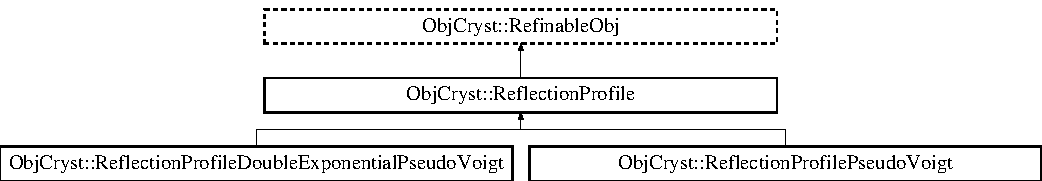
\includegraphics[height=2.000000cm]{a00080}
\end{center}
\end{figure}
\subsubsection*{Public Member Functions}
\begin{DoxyCompactItemize}
\item 
void {\bf X\-M\-L\-Output} (ostream \&os, const string \&name, int indent=0) const 
\begin{DoxyCompactList}\small\item\em X\-M\-L\-Output to stream in well-\/formed X\-M\-L. \end{DoxyCompactList}\item 
void {\bf X\-M\-L\-Output} (ostream \&os, int indent=0) const 
\begin{DoxyCompactList}\small\item\em X\-M\-L\-Output to stream in well-\/formed X\-M\-L. \end{DoxyCompactList}\item 
void {\bf X\-M\-L\-Input} (istream \&is, const {\bf X\-M\-L\-Cryst\-Tag} \&tag)
\begin{DoxyCompactList}\small\item\em X\-M\-L\-Input From stream. \end{DoxyCompactList}\end{DoxyCompactItemize}
\begin{Indent}{\bf Destructor \& Constructors}\par
\begin{DoxyCompactItemize}
\item 
{\bf Refinable\-Par} ()\label{a00080_ae358698d7ab55d87df8af8781946f293}

\begin{DoxyCompactList}\small\item\em Default Constructor. \end{DoxyCompactList}\item 
{\bf Refinable\-Par} (const string \&name, R\-E\-A\-L $\ast$ref\-Par, const R\-E\-A\-L min, const R\-E\-A\-L max, const {\bf Ref\-Par\-Type} $\ast$type, {\bf Ref\-Par\-Deriv\-Step\-Model} deriv\-Mode=R\-E\-F\-P\-A\-R\-\_\-\-D\-E\-R\-I\-V\-\_\-\-S\-T\-E\-P\-\_\-\-R\-E\-L\-A\-T\-I\-V\-E, const bool has\-Limits=true, const bool is\-Fixed=false, const bool is\-Used=true, const bool is\-Periodic=false, const R\-E\-A\-L human\-Scale=1., R\-E\-A\-L period=1.)
\begin{DoxyCompactList}\small\item\em Constructor. \end{DoxyCompactList}\item 
{\bf Refinable\-Par} (const {\bf Refinable\-Par} \&ref)\label{a00080_a99cdc4550c46d90daf63b7f2e6d8d3c3}

\begin{DoxyCompactList}\small\item\em Copy Constructor. \end{DoxyCompactList}\item 
{\bfseries $\sim$\-Refinable\-Par} ()\label{a00080_ada37c0119416edb03732703afaf737a1}

\item 
void {\bf Init} (const string \&name, R\-E\-A\-L $\ast$ref\-Par, const R\-E\-A\-L min, const R\-E\-A\-L max, const {\bf Ref\-Par\-Type} $\ast$type, {\bf Ref\-Par\-Deriv\-Step\-Model} deriv\-Mode=R\-E\-F\-P\-A\-R\-\_\-\-D\-E\-R\-I\-V\-\_\-\-S\-T\-E\-P\-\_\-\-R\-E\-L\-A\-T\-I\-V\-E, const bool has\-Limits=true, const bool is\-Fixed=false, const bool is\-Used=true, const bool is\-Periodic=false, const R\-E\-A\-L human\-Scale=1., R\-E\-A\-L period=1.)
\begin{DoxyCompactList}\small\item\em Constructor. \end{DoxyCompactList}\item 
void {\bf Copy\-Attributes} (const {\bf Refinable\-Par} \&)
\begin{DoxyCompactList}\small\item\em Copy all attributes (limits, flags, etc...) from another \doxyref{Refinable\-Par}{p.}{a00080} object. \end{DoxyCompactList}\end{DoxyCompactItemize}
\end{Indent}
\begin{Indent}{\bf Access \& change the current value of the parameter}\par
\begin{DoxyCompactItemize}
\item 
R\-E\-A\-L {\bf Get\-Value} () const 
\begin{DoxyCompactList}\small\item\em of the parameter. \end{DoxyCompactList}\item 
const R\-E\-A\-L $\ast$ {\bf Get\-Pointer} () const 
\begin{DoxyCompactList}\small\item\em Access to a const pointer to the refined value. \end{DoxyCompactList}\item 
void {\bf Set\-Value} (const R\-E\-A\-L value)
\begin{DoxyCompactList}\small\item\em of the parameter. \end{DoxyCompactList}\item 
const R\-E\-A\-L \& {\bf Get\-Human\-Value} () const \label{a00080_ae1ffe41bcce38c1dc9bf0d649fc06adc}

\begin{DoxyCompactList}\small\item\em Current value of parameter, scaled if necessary (for angles) to a human-\/understandable value. \end{DoxyCompactList}\item 
void {\bf Set\-Human\-Value} (const R\-E\-A\-L \&)\label{a00080_a6bb727ce1de6de9e56c46be1ba75f8b9}

\begin{DoxyCompactList}\small\item\em Current value of parameter, scaled if necessary (for angles) to a human-\/understandable value. \end{DoxyCompactList}\item 
void {\bf Mutate} (const R\-E\-A\-L mutate\-Value)
\begin{DoxyCompactList}\small\item\em Add the given amount to the parameter current value. \end{DoxyCompactList}\item 
void {\bf Mutate\-To} (const R\-E\-A\-L new\-Value)
\begin{DoxyCompactList}\small\item\em Change the current value to the given one. \end{DoxyCompactList}\item 
R\-E\-A\-L {\bfseries Get\-Sigma} () const \label{a00080_aa47f29ee29133f35d3217cfd68b02d57}

\item 
R\-E\-A\-L {\bfseries Get\-Human\-Sigma} () const \label{a00080_a932c8eeab6494b0d67984736560b5b46}

\item 
void {\bfseries Set\-Sigma} (const R\-E\-A\-L)\label{a00080_af199d90bd14333483929aab3a898ae39}

\end{DoxyCompactItemize}
\end{Indent}
\begin{Indent}{\bf General info}\par
\begin{DoxyCompactItemize}
\item 
string {\bf Get\-Name} () const \label{a00080_a0daa7c9ec87518347736e4fa6e45a333}

\begin{DoxyCompactList}\small\item\em Get the parameter's name. \end{DoxyCompactList}\item 
void {\bf Set\-Name} (const string \&)\label{a00080_ac8e91083b8d0c3fe1d3f349122756abb}

\begin{DoxyCompactList}\small\item\em Set the name of the parameter. It should be unique in the \doxyref{Refinable\-Obj}{p.}{a00078}. \end{DoxyCompactList}\item 
void {\bfseries Print} () const \label{a00080_a829f3712a893e3284dfc461d6e7bf016}

\item 
bool {\bfseries Is\-Fixed} () const \label{a00080_a11f0f58b66d069ae9353cd944a0b90ee}

\item 
void {\bfseries Set\-Is\-Fixed} (const bool)\label{a00080_a57690ad69493beb8f2b8976c10833640}

\item 
bool {\bfseries Is\-Limited} () const \label{a00080_ab2421bf2583d6583bc1cf0e1a65ce574}

\item 
void {\bfseries Set\-Is\-Limited} (const bool)\label{a00080_a90c20ed99e6782b6a5abc6d5a6abb105}

\item 
bool {\bf Is\-Used} () const \label{a00080_aa71a1c66f87d910c352286e2ef51c9c9}

\begin{DoxyCompactList}\small\item\em Is the parameter used (if not, it is simply irrelevant in the model) ? \end{DoxyCompactList}\item 
void {\bf Set\-Is\-Used} (const bool)\label{a00080_aea29e6822f1a6215c274cacf5c58e7ce}

\begin{DoxyCompactList}\small\item\em Is the parameter used (if not, it is simply irrelevant in the model) ? \end{DoxyCompactList}\item 
bool {\bfseries Is\-Periodic} () const \label{a00080_a886b2db23080365ef90870e846a27dfa}

\item 
void {\bfseries Set\-Is\-Periodic} (const bool, R\-E\-A\-L period=1)\label{a00080_a3e131a39649e853afb121ce5c9b5ebe1}

\item 
R\-E\-A\-L {\bf Get\-Human\-Scale} () const \label{a00080_a97fb48bd2b4d6845d5543573dad84aea}

\begin{DoxyCompactList}\small\item\em Human scale for this parameter \-: for angles, this is equal to 180/pi. \end{DoxyCompactList}\item 
void {\bf Set\-Human\-Scale} (const R\-E\-A\-L)\label{a00080_a05a23549ca32b4745dee0a1bb539830e}

\begin{DoxyCompactList}\small\item\em Human scale for this parameter \-: for angles, this is equal to 180/pi. \end{DoxyCompactList}\end{DoxyCompactItemize}
\end{Indent}
\begin{Indent}{\bf Min, max values}\par
\begin{DoxyCompactItemize}
\item 
R\-E\-A\-L {\bf Get\-Min} () const \label{a00080_a27d046a98b774ff373aec8a6aeca31ae}

\begin{DoxyCompactList}\small\item\em Minimum value allowed (if limited or periodic) \end{DoxyCompactList}\item 
void {\bf Set\-Min} (const R\-E\-A\-L)\label{a00080_a82ece8fe469cfc3582f7d5d899928630}

\begin{DoxyCompactList}\small\item\em Set the Minimum value allowed (if limited) \end{DoxyCompactList}\item 
R\-E\-A\-L {\bf Get\-Human\-Min} () const \label{a00080_a8f9a61e06332dd459ed55c117b9c7475}

\begin{DoxyCompactList}\small\item\em Get the minimum value allowed (if limited) \end{DoxyCompactList}\item 
void {\bf Set\-Human\-Min} (const R\-E\-A\-L)\label{a00080_ad4ba7c4c6d1c46c9334dcc0673df4fb2}

\begin{DoxyCompactList}\small\item\em Set the minimum value allowed (if limited) \end{DoxyCompactList}\item 
R\-E\-A\-L {\bf Get\-Max} () const \label{a00080_ab1e49d10dd00c3ba156d2adb9d0dc6b3}

\begin{DoxyCompactList}\small\item\em Get the maximum value allowed (if limited) \end{DoxyCompactList}\item 
void {\bf Set\-Max} (const R\-E\-A\-L)\label{a00080_a33f45d527d405da957ddc513e5a3099f}

\begin{DoxyCompactList}\small\item\em Get the maximum value allowed (if limited) \end{DoxyCompactList}\item 
R\-E\-A\-L {\bf Get\-Human\-Max} () const \label{a00080_ad4a7468d788806cd893fcca83534eb83}

\begin{DoxyCompactList}\small\item\em Get the maximum value allowed (if limited) \end{DoxyCompactList}\item 
void {\bf Set\-Human\-Max} (const R\-E\-A\-L)\label{a00080_ade6c83881319be43feb679b4896766bd}

\begin{DoxyCompactList}\small\item\em Get the maximum value allowed (if limited) \end{DoxyCompactList}\item 
R\-E\-A\-L {\bf Get\-Period} () const \label{a00080_a2bc0ba973f3e0e5eb93be0a0ebc29c93}

\begin{DoxyCompactList}\small\item\em Get the period (if periodic) \end{DoxyCompactList}\item 
void {\bf Set\-Period} (const R\-E\-A\-L)\label{a00080_a97b23ea6b624bbe517c29b5ef00b5f5b}

\begin{DoxyCompactList}\small\item\em Set the period value (if periodic) \end{DoxyCompactList}\end{DoxyCompactItemize}
\end{Indent}
\begin{Indent}{\bf Steps during refinement}\par
\begin{DoxyCompactItemize}
\item 
R\-E\-A\-L {\bf Get\-Deriv\-Step} () const \label{a00080_a8ba4cbee715d51c85ce5147ce9cf45db}

\begin{DoxyCompactList}\small\item\em Fixed step to use to compute numerical derivative. \end{DoxyCompactList}\item 
void {\bf Set\-Deriv\-Step} (const R\-E\-A\-L)\label{a00080_a3156b809e45a6314a680bbe3dec1a573}

\begin{DoxyCompactList}\small\item\em Fixed step to use to compute numerical derivative. \end{DoxyCompactList}\item 
R\-E\-A\-L {\bf Get\-Global\-Optim\-Step} () const \label{a00080_a2fb1982abc56de79e7dd79ee6bbd0e3f}

\begin{DoxyCompactList}\small\item\em Maximum step to use during Global Optimization algorithms. \end{DoxyCompactList}\item 
void {\bf Set\-Global\-Optim\-Step} (const R\-E\-A\-L)\label{a00080_aa0eccaf87210097fb9e5239a97f9dcd1}

\begin{DoxyCompactList}\small\item\em Maximum step to use during Global Optimization algorithms. \end{DoxyCompactList}\end{DoxyCompactItemize}
\end{Indent}
\begin{Indent}{\bf Parameter's Clock}\par
\begin{DoxyCompactItemize}
\item 
void {\bf Assign\-Clock} ({\bf Refinable\-Obj\-Clock} \&clock)
\item 
const {\bf Refinable\-Obj\-Clock} \& {\bf Get\-Clock} () const \label{a00080_a18c0d07d6795a1016af3bda5cca694a2}

\begin{DoxyCompactList}\small\item\em Get a constant reference to the clock assigned to this parameter. \end{DoxyCompactList}\item 
{\bf Refinable\-Obj\-Clock} \& {\bf Get\-Clock} ()\label{a00080_ad6495758297cf923c8746cb3734fc838}

\begin{DoxyCompactList}\small\item\em Get a reference to the clock assigned to this parameter. \end{DoxyCompactList}\end{DoxyCompactItemize}
\end{Indent}
\begin{Indent}{\bf Change Limits}\par
\begin{DoxyCompactItemize}
\item 
void {\bf Set\-Limits\-Absolute} (const R\-E\-A\-L min, const R\-E\-A\-L max)\label{a00080_aad4275aa946de7b60aaf3353971663dd}

\begin{DoxyCompactList}\small\item\em Change the limits for this object, giving absolute new limits. \end{DoxyCompactList}\item 
void {\bf Set\-Limits\-Relative} (const R\-E\-A\-L min, const R\-E\-A\-L max)
\begin{DoxyCompactList}\small\item\em Change the limits for this object, giving relative new limits (eg giving -\/.\-1 and +.1 will set new limits at the current value + min and current value + max) Thus min should logically be $<$0 and max $>$0. \end{DoxyCompactList}\item 
void {\bf Set\-Limits\-Proportional} (const R\-E\-A\-L min, const R\-E\-A\-L max)
\begin{DoxyCompactList}\small\item\em Change the limits for this object, proportionnaly to the current value. \end{DoxyCompactList}\end{DoxyCompactItemize}
\end{Indent}
\subsubsection*{Private Member Functions}
\begin{DoxyCompactItemize}
\item 
void {\bf Click} ()\label{a00080_a3dc5a8cf7fb9d3c800fe6dd494054d92}

\begin{DoxyCompactList}\small\item\em Click the Clock ! to telle the \doxyref{Refinable\-Obj}{p.}{a00078} it has been modified. \end{DoxyCompactList}\end{DoxyCompactItemize}
\subsubsection*{Private Attributes}
\begin{DoxyCompactItemize}
\item 
string {\bf m\-Name}\label{a00080_afe5091b81dec1c77b7ec98f473f40698}

\begin{DoxyCompactList}\small\item\em name of the refinable parameter \end{DoxyCompactList}\item 
R\-E\-A\-L $\ast$ {\bf mp\-Value}\label{a00080_a8bfbe4ae25c98850480c70a2cde259dc}

\begin{DoxyCompactList}\small\item\em Pointer to the refinable value. \end{DoxyCompactList}\item 
R\-E\-A\-L {\bf m\-Min}\label{a00080_a303f811dfa1a8592ed2a72c489eabe1e}

\begin{DoxyCompactList}\small\item\em Hard lower and upper limits. \end{DoxyCompactList}\item 
R\-E\-A\-L {\bfseries m\-Max}\label{a00080_ae16a4a1d93b0f86e683f2a51ab4d627f}

\item 
bool {\bf m\-Has\-Limits}\label{a00080_a867316e66708e8d7efb64b9064f5241a}

\begin{DoxyCompactList}\small\item\em Does the refinable parameter need limits (min and max) ? \end{DoxyCompactList}\item 
bool {\bf m\-Is\-Fixed}\label{a00080_acf1638fe7459af0df2f64279115f6091}

\begin{DoxyCompactList}\small\item\em is the parameter currently fixed ? \end{DoxyCompactList}\item 
bool {\bf m\-Is\-Used}\label{a00080_a9d6d609d62226ba7c6fe1a1fd694b77d}

\begin{DoxyCompactList}\small\item\em Is the parameter currently used ? \end{DoxyCompactList}\item 
bool {\bf m\-Is\-Periodic}
\begin{DoxyCompactList}\small\item\em Is the parameter periodic ? If this is the case, then when using the \doxyref{Refinable\-Par\-::\-Mutate()}{p.}{a00080_abd6a06bbb5eb59d80515ebdad2612da8} function, if the parameter goes beyond its limits, it will be shifted by the value of its period. \end{DoxyCompactList}\item 
R\-E\-A\-L {\bf m\-Period}\label{a00080_ae33430ff688a0a5e4e907ab8bbee0ecd}

\begin{DoxyCompactList}\small\item\em Period value (if relevant) \end{DoxyCompactList}\item 
R\-E\-A\-L {\bf m\-Global\-Optim\-Step}\label{a00080_a3d5465cf22c3080f856825c29f45e201}

\begin{DoxyCompactList}\small\item\em Step to use for global method search (simulated annealing,...) \end{DoxyCompactList}\item 
R\-E\-A\-L {\bf m\-Deriv\-Step}\label{a00080_a07c0acd9afc24e5945bfa8a9e940002d}

\begin{DoxyCompactList}\small\item\em Step to use for numerical derivative calculation. \end{DoxyCompactList}\item 
{\bf Ref\-Par\-Deriv\-Step\-Model} {\bf m\-Ref\-Par\-Deriv\-Step\-Model}\label{a00080_adb6f88fa2781510eef3e024accda52ed}

\begin{DoxyCompactList}\small\item\em Model followed for derivation. \end{DoxyCompactList}\item 
R\-E\-A\-L {\bf m\-Sigma}\label{a00080_a943363b2a00d01575668ad6d3e27dafb}

\begin{DoxyCompactList}\small\item\em Calculated sigma on value. \end{DoxyCompactList}\item 
R\-E\-A\-L {\bf m\-Human\-Scale}
\begin{DoxyCompactList}\small\item\em Scale to be used to display 'human' value. \end{DoxyCompactList}\item 
bool {\bf m\-Has\-Assigned\-Clock}\label{a00080_a32ec16db6ad86efc4bd14dcfbb0e9712}

\begin{DoxyCompactList}\small\item\em Is there a clock associated with this parameter ? If yes, then it must \doxyref{Click()}{p.}{a00080_a3dc5a8cf7fb9d3c800fe6dd494054d92} it each time it is modified. \end{DoxyCompactList}\item 
{\bf Refinable\-Obj\-Clock} $\ast$ {\bfseries mp\-Clock}\label{a00080_a3c6145e3df75637040f0b2e64ec00382}

\end{DoxyCompactItemize}
\subsubsection*{Friends}
\begin{DoxyCompactItemize}
\item 
class {\bfseries Refinable\-Obj}\label{a00080_a4b004207cfa15cef5b32be20104e3eaf}

\end{DoxyCompactItemize}


\subsubsection{Detailed Description}
Generic class for parameters of refinable objects. 

These must be continuous.

\begin{DoxyRefDesc}{Todo}
\item[{\bf Todo}]\-: define parameters using equations between parameters. 

\-: for complex objects with lots of parameters, give the possibility to define vectors of parameters, all with the same properties, to reduce memory usage. \end{DoxyRefDesc}


\subsubsection{Constructor \& Destructor Documentation}
\index{Obj\-Cryst\-::\-Refinable\-Par@{Obj\-Cryst\-::\-Refinable\-Par}!Refinable\-Par@{Refinable\-Par}}
\index{Refinable\-Par@{Refinable\-Par}!ObjCryst::RefinablePar@{Obj\-Cryst\-::\-Refinable\-Par}}
\paragraph[{Refinable\-Par}]{\setlength{\rightskip}{0pt plus 5cm}Obj\-Cryst\-::\-Refinable\-Par\-::\-Refinable\-Par (
\begin{DoxyParamCaption}
\item[{const string \&}]{name, }
\item[{R\-E\-A\-L $\ast$}]{ref\-Par, }
\item[{const R\-E\-A\-L}]{min, }
\item[{const R\-E\-A\-L}]{max, }
\item[{const {\bf Ref\-Par\-Type} $\ast$}]{type, }
\item[{{\bf Ref\-Par\-Deriv\-Step\-Model}}]{deriv\-Mode = {\ttfamily REFPAR\-\_\-DERIV\-\_\-STEP\-\_\-RELATIVE}, }
\item[{const bool}]{has\-Limits = {\ttfamily true}, }
\item[{const bool}]{is\-Fixed = {\ttfamily false}, }
\item[{const bool}]{is\-Used = {\ttfamily true}, }
\item[{const bool}]{is\-Periodic = {\ttfamily false}, }
\item[{const R\-E\-A\-L}]{human\-Scale = {\ttfamily 1.}, }
\item[{R\-E\-A\-L}]{period = {\ttfamily 1.}}
\end{DoxyParamCaption}
)}\label{a00080_ac82759679653390c868ca7cbcb7e572c}


Constructor. 

\begin{DoxyParagraph}{name\-: the name of the parameter}

\end{DoxyParagraph}
\begin{DoxyParagraph}{ref\-Par\-: the address of the refined parameter}

\end{DoxyParagraph}
\begin{DoxyParagraph}{min,max\-: the minimum \& maximum value for this parameter. Only used}
if the parameter is limited. 
\end{DoxyParagraph}
\begin{DoxyParagraph}{type\-: the type (category) of refinable parameter. This is used to (de)activate}
groups of parameters. 
\end{DoxyParagraph}
\begin{DoxyParagraph}{deriv\-Mode\-: to compute numerical (partial) derivatives, the step used is either}
an absolute (fixed) value, or it can be proportionnal to the current value of the parameter. 
\end{DoxyParagraph}
\begin{DoxyParagraph}{has\-Limits\-: if true, then the parameter cannot exceed its limits.}

\end{DoxyParagraph}
\begin{DoxyParagraph}{is\-Fixed\-: if true, the parameter cannot be refined.}

\end{DoxyParagraph}
\begin{DoxyParagraph}{is\-Used\-: if false, then the parameter does not affect in any way the refined object,}
and thus is simply ignored and should never appear to the user. 
\end{DoxyParagraph}
\begin{DoxyParagraph}{is\-Periodic\-: if true, then when the parameter exceeds one of its limits, it is}
shifted by the period (=max-\/min), in order to be back to the allowed [min,max] range. 
\end{DoxyParagraph}
\begin{DoxyParagraph}{human\-Scale\-:this is the scale which should be used to display the value to the}
end program user. This is mostly used for angles\-: the values are stored in radians, so that a scale equal to 180/pi must be used for a 'human-\/understandable' value. Use the Refinable\-Par\-::\-Human\-Value() in order to get this value. By default it is equal to 1.\-0 (no scaling required). 
\end{DoxyParagraph}


\subsubsection{Member Function Documentation}
\index{Obj\-Cryst\-::\-Refinable\-Par@{Obj\-Cryst\-::\-Refinable\-Par}!Assign\-Clock@{Assign\-Clock}}
\index{Assign\-Clock@{Assign\-Clock}!ObjCryst::RefinablePar@{Obj\-Cryst\-::\-Refinable\-Par}}
\paragraph[{Assign\-Clock}]{\setlength{\rightskip}{0pt plus 5cm}void Obj\-Cryst\-::\-Refinable\-Par\-::\-Assign\-Clock (
\begin{DoxyParamCaption}
\item[{{\bf Refinable\-Obj\-Clock} \&}]{clock}
\end{DoxyParamCaption}
)}\label{a00080_ab03f6bffb78dd812136a73b94b64ee6e}
Assign a clock to this parameter. Any time this parameter is modified, the clock will be ticked ! \index{Obj\-Cryst\-::\-Refinable\-Par@{Obj\-Cryst\-::\-Refinable\-Par}!Copy\-Attributes@{Copy\-Attributes}}
\index{Copy\-Attributes@{Copy\-Attributes}!ObjCryst::RefinablePar@{Obj\-Cryst\-::\-Refinable\-Par}}
\paragraph[{Copy\-Attributes}]{\setlength{\rightskip}{0pt plus 5cm}void Obj\-Cryst\-::\-Refinable\-Par\-::\-Copy\-Attributes (
\begin{DoxyParamCaption}
\item[{const {\bf Refinable\-Par} \&}]{}
\end{DoxyParamCaption}
)}\label{a00080_a5882aec9561125f6e81b81f175031652}


Copy all attributes (limits, flags, etc...) from another \doxyref{Refinable\-Par}{p.}{a00080} object. 

This is useful in \doxyref{Refinable\-Obj}{p.}{a00078} copy constructors. Everything is copied but the pointer to the value refined, and the pointer to the clock. \index{Obj\-Cryst\-::\-Refinable\-Par@{Obj\-Cryst\-::\-Refinable\-Par}!Get\-Pointer@{Get\-Pointer}}
\index{Get\-Pointer@{Get\-Pointer}!ObjCryst::RefinablePar@{Obj\-Cryst\-::\-Refinable\-Par}}
\paragraph[{Get\-Pointer}]{\setlength{\rightskip}{0pt plus 5cm}const R\-E\-A\-L$\ast$ Obj\-Cryst\-::\-Refinable\-Par\-::\-Get\-Pointer (
\begin{DoxyParamCaption}
{}
\end{DoxyParamCaption}
) const}\label{a00080_a128e04b0731ed791ecc3afc228d6f17e}


Access to a const pointer to the refined value. 

This can be used to identify the parameter \index{Obj\-Cryst\-::\-Refinable\-Par@{Obj\-Cryst\-::\-Refinable\-Par}!Get\-Value@{Get\-Value}}
\index{Get\-Value@{Get\-Value}!ObjCryst::RefinablePar@{Obj\-Cryst\-::\-Refinable\-Par}}
\paragraph[{Get\-Value}]{\setlength{\rightskip}{0pt plus 5cm}R\-E\-A\-L Obj\-Cryst\-::\-Refinable\-Par\-::\-Get\-Value (
\begin{DoxyParamCaption}
{}
\end{DoxyParamCaption}
) const}\label{a00080_ad27e4b5ed56bdf316c8d322537a7c85a}


of the parameter. 

Use the The \doxyref{Mutate()}{p.}{a00080_abd6a06bbb5eb59d80515ebdad2612da8} and \doxyref{Mutate\-To()}{p.}{a00080_a696f87a0a129cfd270144532d664d093} function to change this value. \index{Obj\-Cryst\-::\-Refinable\-Par@{Obj\-Cryst\-::\-Refinable\-Par}!Init@{Init}}
\index{Init@{Init}!ObjCryst::RefinablePar@{Obj\-Cryst\-::\-Refinable\-Par}}
\paragraph[{Init}]{\setlength{\rightskip}{0pt plus 5cm}void Obj\-Cryst\-::\-Refinable\-Par\-::\-Init (
\begin{DoxyParamCaption}
\item[{const string \&}]{name, }
\item[{R\-E\-A\-L $\ast$}]{ref\-Par, }
\item[{const R\-E\-A\-L}]{min, }
\item[{const R\-E\-A\-L}]{max, }
\item[{const {\bf Ref\-Par\-Type} $\ast$}]{type, }
\item[{{\bf Ref\-Par\-Deriv\-Step\-Model}}]{deriv\-Mode = {\ttfamily REFPAR\-\_\-DERIV\-\_\-STEP\-\_\-RELATIVE}, }
\item[{const bool}]{has\-Limits = {\ttfamily true}, }
\item[{const bool}]{is\-Fixed = {\ttfamily false}, }
\item[{const bool}]{is\-Used = {\ttfamily true}, }
\item[{const bool}]{is\-Periodic = {\ttfamily false}, }
\item[{const R\-E\-A\-L}]{human\-Scale = {\ttfamily 1.}, }
\item[{R\-E\-A\-L}]{period = {\ttfamily 1.}}
\end{DoxyParamCaption}
)}\label{a00080_a58cbd1b3c3ada8383ddb444f879a9495}


Constructor. 

\begin{DoxyParagraph}{name\-: the name of the parameter}

\end{DoxyParagraph}
\begin{DoxyParagraph}{ref\-Par\-: the address of the refined parameter}

\end{DoxyParagraph}
\begin{DoxyParagraph}{min,max\-: the minimum \& maximum value for this parameter. Only used}
if the parameter is limited. 
\end{DoxyParagraph}
\begin{DoxyParagraph}{type\-: the type (category) of refinable parameter. This is used to (de)activate}
groups of parameters. 
\end{DoxyParagraph}
\begin{DoxyParagraph}{deriv\-Mode\-: to compute numerical (partial) derivatives, the step used is either}
an absolute (fixed) value, or it can be proportionnal to the current value of the parameter. 
\end{DoxyParagraph}
\begin{DoxyParagraph}{has\-Limits\-: if true, then the parameter cannot exceed its limits.}

\end{DoxyParagraph}
\begin{DoxyParagraph}{is\-Fixed\-: if true, the parameter cannot be refined.}

\end{DoxyParagraph}
\begin{DoxyParagraph}{is\-Used\-: if false, then the parameter does not affect in any way the refined object,}
and thus is simply ignored and should never appear to the user. 
\end{DoxyParagraph}
\begin{DoxyParagraph}{is\-Periodic\-: if true, then when the parameter exceeds one of its limits, it is}
shifted by the period (=max-\/min), in order to be back to the allowed [min,max] range. 
\end{DoxyParagraph}
\begin{DoxyParagraph}{human\-Scale\-:this is the scale which should be used to display the value to the}
end program user. This is mostly used for angles\-: the values are stored in radians, so that a scale equal to 180/pi must be used for a 'human-\/understandable' value. Use the Refinable\-Par\-::\-Human\-Value() in order to get this value. By default it is equal to 1.\-0 (no scaling required). 
\end{DoxyParagraph}
\index{Obj\-Cryst\-::\-Refinable\-Par@{Obj\-Cryst\-::\-Refinable\-Par}!Mutate@{Mutate}}
\index{Mutate@{Mutate}!ObjCryst::RefinablePar@{Obj\-Cryst\-::\-Refinable\-Par}}
\paragraph[{Mutate}]{\setlength{\rightskip}{0pt plus 5cm}void Obj\-Cryst\-::\-Refinable\-Par\-::\-Mutate (
\begin{DoxyParamCaption}
\item[{const R\-E\-A\-L}]{mutate\-Value}
\end{DoxyParamCaption}
)}\label{a00080_abd6a06bbb5eb59d80515ebdad2612da8}


Add the given amount to the parameter current value. 

If limit is hit, set to limit. If the limit is hit {\itshape and} the parameter is periodic, shift by period to bring back to allowed values. \begin{DoxyWarning}{Warning}
Will throw an exception if the parameter is defined by an equation. 
\end{DoxyWarning}
\index{Obj\-Cryst\-::\-Refinable\-Par@{Obj\-Cryst\-::\-Refinable\-Par}!Mutate\-To@{Mutate\-To}}
\index{Mutate\-To@{Mutate\-To}!ObjCryst::RefinablePar@{Obj\-Cryst\-::\-Refinable\-Par}}
\paragraph[{Mutate\-To}]{\setlength{\rightskip}{0pt plus 5cm}void Obj\-Cryst\-::\-Refinable\-Par\-::\-Mutate\-To (
\begin{DoxyParamCaption}
\item[{const R\-E\-A\-L}]{new\-Value}
\end{DoxyParamCaption}
)}\label{a00080_a696f87a0a129cfd270144532d664d093}


Change the current value to the given one. 

If the limit is hit, then set to the limit (unless the pameter is periodic, then shift by the period amount back to allowed values). \begin{DoxyWarning}{Warning}
Will throw an exception if the parameter is defined by an equation. 
\end{DoxyWarning}
\index{Obj\-Cryst\-::\-Refinable\-Par@{Obj\-Cryst\-::\-Refinable\-Par}!Set\-Limits\-Proportional@{Set\-Limits\-Proportional}}
\index{Set\-Limits\-Proportional@{Set\-Limits\-Proportional}!ObjCryst::RefinablePar@{Obj\-Cryst\-::\-Refinable\-Par}}
\paragraph[{Set\-Limits\-Proportional}]{\setlength{\rightskip}{0pt plus 5cm}void Obj\-Cryst\-::\-Refinable\-Par\-::\-Set\-Limits\-Proportional (
\begin{DoxyParamCaption}
\item[{const R\-E\-A\-L}]{min, }
\item[{const R\-E\-A\-L}]{max}
\end{DoxyParamCaption}
)}\label{a00080_afb15606bb24a5fbb144d07843bb11f97}


Change the limits for this object, proportionnaly to the current value. 

min should be $<$ 1. and max $>$ 1. \index{Obj\-Cryst\-::\-Refinable\-Par@{Obj\-Cryst\-::\-Refinable\-Par}!Set\-Limits\-Relative@{Set\-Limits\-Relative}}
\index{Set\-Limits\-Relative@{Set\-Limits\-Relative}!ObjCryst::RefinablePar@{Obj\-Cryst\-::\-Refinable\-Par}}
\paragraph[{Set\-Limits\-Relative}]{\setlength{\rightskip}{0pt plus 5cm}void Obj\-Cryst\-::\-Refinable\-Par\-::\-Set\-Limits\-Relative (
\begin{DoxyParamCaption}
\item[{const R\-E\-A\-L}]{min, }
\item[{const R\-E\-A\-L}]{max}
\end{DoxyParamCaption}
)}\label{a00080_ad445354c927f8df95443a55174e7bb7d}


Change the limits for this object, giving relative new limits (eg giving -\/.\-1 and +.1 will set new limits at the current value + min and current value + max) Thus min should logically be $<$0 and max $>$0. 

\index{Obj\-Cryst\-::\-Refinable\-Par@{Obj\-Cryst\-::\-Refinable\-Par}!Set\-Value@{Set\-Value}}
\index{Set\-Value@{Set\-Value}!ObjCryst::RefinablePar@{Obj\-Cryst\-::\-Refinable\-Par}}
\paragraph[{Set\-Value}]{\setlength{\rightskip}{0pt plus 5cm}void Obj\-Cryst\-::\-Refinable\-Par\-::\-Set\-Value (
\begin{DoxyParamCaption}
\item[{const R\-E\-A\-L}]{value}
\end{DoxyParamCaption}
)}\label{a00080_a55a87d842fc046b2f4b3c03c92e53052}


of the parameter. 

Use the The \doxyref{Mutate()}{p.}{a00080_abd6a06bbb5eb59d80515ebdad2612da8} and \doxyref{Mutate\-To()}{p.}{a00080_a696f87a0a129cfd270144532d664d093} function to change this value. \index{Obj\-Cryst\-::\-Refinable\-Par@{Obj\-Cryst\-::\-Refinable\-Par}!X\-M\-L\-Input@{X\-M\-L\-Input}}
\index{X\-M\-L\-Input@{X\-M\-L\-Input}!ObjCryst::RefinablePar@{Obj\-Cryst\-::\-Refinable\-Par}}
\paragraph[{X\-M\-L\-Input}]{\setlength{\rightskip}{0pt plus 5cm}void Obj\-Cryst\-::\-Refinable\-Par\-::\-X\-M\-L\-Input (
\begin{DoxyParamCaption}
\item[{istream \&}]{is, }
\item[{const {\bf X\-M\-L\-Cryst\-Tag} \&}]{tag}
\end{DoxyParamCaption}
)}\label{a00080_af6fcabe9e97e0aabacef7a9bee5d1106}


X\-M\-L\-Input From stream. 

\index{Obj\-Cryst\-::\-Refinable\-Par@{Obj\-Cryst\-::\-Refinable\-Par}!X\-M\-L\-Output@{X\-M\-L\-Output}}
\index{X\-M\-L\-Output@{X\-M\-L\-Output}!ObjCryst::RefinablePar@{Obj\-Cryst\-::\-Refinable\-Par}}
\paragraph[{X\-M\-L\-Output}]{\setlength{\rightskip}{0pt plus 5cm}void Obj\-Cryst\-::\-Refinable\-Par\-::\-X\-M\-L\-Output (
\begin{DoxyParamCaption}
\item[{ostream \&}]{os, }
\item[{const string \&}]{name, }
\item[{int}]{indent = {\ttfamily 0}}
\end{DoxyParamCaption}
) const}\label{a00080_ae8271536206b603c717c5fa793b2310c}


X\-M\-L\-Output to stream in well-\/formed X\-M\-L. 

this will save the fixed \& limited flags, as well as limits 
\begin{DoxyParams}{Parameters}
{\em name} & the name to use instead of the Ref\-Par name. \\
\hline
\end{DoxyParams}
\index{Obj\-Cryst\-::\-Refinable\-Par@{Obj\-Cryst\-::\-Refinable\-Par}!X\-M\-L\-Output@{X\-M\-L\-Output}}
\index{X\-M\-L\-Output@{X\-M\-L\-Output}!ObjCryst::RefinablePar@{Obj\-Cryst\-::\-Refinable\-Par}}
\paragraph[{X\-M\-L\-Output}]{\setlength{\rightskip}{0pt plus 5cm}void Obj\-Cryst\-::\-Refinable\-Par\-::\-X\-M\-L\-Output (
\begin{DoxyParamCaption}
\item[{ostream \&}]{os, }
\item[{int}]{indent = {\ttfamily 0}}
\end{DoxyParamCaption}
) const}\label{a00080_a7105a845ac12a49b0a5fcb41a4e6cbde}


X\-M\-L\-Output to stream in well-\/formed X\-M\-L. 

this will save the fixed \& limited flags, as well as limits. In this function the name used is that of the Ref\-Par. 

\subsubsection{Member Data Documentation}
\index{Obj\-Cryst\-::\-Refinable\-Par@{Obj\-Cryst\-::\-Refinable\-Par}!m\-Human\-Scale@{m\-Human\-Scale}}
\index{m\-Human\-Scale@{m\-Human\-Scale}!ObjCryst::RefinablePar@{Obj\-Cryst\-::\-Refinable\-Par}}
\paragraph[{m\-Human\-Scale}]{\setlength{\rightskip}{0pt plus 5cm}R\-E\-A\-L Obj\-Cryst\-::\-Refinable\-Par\-::m\-Human\-Scale\hspace{0.3cm}{\ttfamily [private]}}\label{a00080_a1a0b4a89d0d106fe43d4ada7c44e4cd9}


Scale to be used to display 'human' value. 

This is for angular parameters\-: the computer stores values in radians, whil the user only understands degrees. So a scale factor of 180/pi is necessary. \index{Obj\-Cryst\-::\-Refinable\-Par@{Obj\-Cryst\-::\-Refinable\-Par}!m\-Is\-Periodic@{m\-Is\-Periodic}}
\index{m\-Is\-Periodic@{m\-Is\-Periodic}!ObjCryst::RefinablePar@{Obj\-Cryst\-::\-Refinable\-Par}}
\paragraph[{m\-Is\-Periodic}]{\setlength{\rightskip}{0pt plus 5cm}bool Obj\-Cryst\-::\-Refinable\-Par\-::m\-Is\-Periodic\hspace{0.3cm}{\ttfamily [private]}}\label{a00080_a15b4dfefc764d205251606a64155b677}


Is the parameter periodic ? If this is the case, then when using the \doxyref{Refinable\-Par\-::\-Mutate()}{p.}{a00080_abd6a06bbb5eb59d80515ebdad2612da8} function, if the parameter goes beyond its limits, it will be shifted by the value of its period. 



The documentation for this class was generated from the following file\-:\begin{DoxyCompactItemize}
\item 
Refinable\-Obj.\-h\end{DoxyCompactItemize}

\subsection{Obj\+Cryst\+:\+:Reflection\+Profile\+Double\+Exponential\+Pseudo\+Voigt Class Reference}
\label{a00081}\index{Obj\+Cryst\+::\+Reflection\+Profile\+Double\+Exponential\+Pseudo\+Voigt@{Obj\+Cryst\+::\+Reflection\+Profile\+Double\+Exponential\+Pseudo\+Voigt}}


Double-\/\+Exponential Pseudo-\/\+Voigt profile for T\+O\+F.  


Inheritance diagram for Obj\+Cryst\+:\+:Reflection\+Profile\+Double\+Exponential\+Pseudo\+Voigt\+:\begin{figure}[H]
\begin{center}
\leavevmode
\includegraphics[height=3.000000cm]{a00081}
\end{center}
\end{figure}
\subsubsection*{Public Member Functions}
\begin{DoxyCompactItemize}
\item 
{\bf Reflection\+Profile\+Double\+Exponential\+Pseudo\+Voigt} ()\label{a00081_a99d69f5a755094081165c27f8cbc0de2}

\begin{DoxyCompactList}\small\item\em Constructor, without unit cell. \end{DoxyCompactList}\item 
{\bf Reflection\+Profile\+Double\+Exponential\+Pseudo\+Voigt} (const {\bf Unit\+Cell} \&cell)\label{a00081_a83ca292045467ce5ca2fd5f33f60082b}

\begin{DoxyCompactList}\small\item\em Constructor, with unit cell. \end{DoxyCompactList}\item 
{\bfseries Reflection\+Profile\+Double\+Exponential\+Pseudo\+Voigt} (const {\bf Reflection\+Profile\+Double\+Exponential\+Pseudo\+Voigt} \&old)\label{a00081_ae4b01c3514699b3ca8981776afd11010}

\item 
virtual \\*
{\bf Reflection\+Profile\+Double\+Exponential\+Pseudo\+Voigt} $\ast$ {\bfseries Create\+Copy} () const \label{a00081_a495f3877130c4afa1f7456d962b62407}

\item 
virtual const string \& {\bf Get\+Class\+Name} () const 
\begin{DoxyCompactList}\small\item\em Name for this class (\char`\"{}\+Refinable\+Obj\char`\"{}, \char`\"{}\+Crystal\char`\"{},...). \end{DoxyCompactList}\item 
Cryst\+Vector\+\_\+\+R\+E\+A\+L {\bf Get\+Profile} (const Cryst\+Vector\+\_\+\+R\+E\+A\+L \&x, const R\+E\+A\+L xcenter, const R\+E\+A\+L h, const R\+E\+A\+L k, const R\+E\+A\+L l)
\begin{DoxyCompactList}\small\item\em Get the reflection profile. \end{DoxyCompactList}\item 
void {\bf Set\+Profile\+Par} (const R\+E\+A\+L instrument\+Alpha0, const R\+E\+A\+L instrument\+Alpha1, const R\+E\+A\+L instrument\+Beta0, const R\+E\+A\+L instrument\+Beta1, const R\+E\+A\+L gaussian\+Sigma0, const R\+E\+A\+L gaussian\+Sigma1, const R\+E\+A\+L gaussian\+Sigma2, const R\+E\+A\+L lorentzian\+Gamma0, const R\+E\+A\+L lorentzian\+Gamma1, const R\+E\+A\+L lorentzian\+Gamma2)
\begin{DoxyCompactList}\small\item\em Set reflection profile parameters. \end{DoxyCompactList}\item 
virtual R\+E\+A\+L {\bf Get\+Full\+Profile\+Width} (const R\+E\+A\+L relative\+Intensity, const R\+E\+A\+L xcenter, const R\+E\+A\+L h, const R\+E\+A\+L k, const R\+E\+A\+L l)
\begin{DoxyCompactList}\small\item\em Get the (approximate) full profile width at a given percentage of the profile maximum (e.\+g. \end{DoxyCompactList}\item 
bool {\bf Is\+Anisotropic} () const \label{a00081_a912e47b21ac000e04385058a183aba9b}

\begin{DoxyCompactList}\small\item\em Is the profile anisotropic ? \end{DoxyCompactList}\item 
virtual void {\bf X\+M\+L\+Output} (ostream \&os, int indent=0) const 
\begin{DoxyCompactList}\small\item\em Output to stream in well-\/formed X\+M\+L. \end{DoxyCompactList}\item 
virtual void {\bf X\+M\+L\+Input} (istream \&is, const {\bf X\+M\+L\+Cryst\+Tag} \&tag)
\begin{DoxyCompactList}\small\item\em Input From stream. \end{DoxyCompactList}\item 
void {\bf Set\+Unit\+Cell} (const {\bf Unit\+Cell} \&cell)
\begin{DoxyCompactList}\small\item\em Set unit cell. \end{DoxyCompactList}\end{DoxyCompactItemize}
\subsubsection*{Private Member Functions}
\begin{DoxyCompactItemize}
\item 
void {\bf Init\+Parameters} ()\label{a00081_a32fe8cd36500837396f2ac7070b9f841}

\begin{DoxyCompactList}\small\item\em Initialize parameters. \end{DoxyCompactList}\end{DoxyCompactItemize}
\subsubsection*{Private Attributes}
\begin{DoxyCompactItemize}
\item 
R\+E\+A\+L {\bfseries m\+Instrument\+Alpha0}\label{a00081_a93fd2450116ca2461fcffc08a2d8e674}

\item 
R\+E\+A\+L {\bfseries m\+Instrument\+Alpha1}\label{a00081_a35157f2ea58bd0f5f6ad1620ea227078}

\item 
R\+E\+A\+L {\bfseries m\+Instrument\+Beta0}\label{a00081_af385ee3d583f76cef00990878844a597}

\item 
R\+E\+A\+L {\bfseries m\+Instrument\+Beta1}\label{a00081_a98ce27de2255899ebd7421298b718eb2}

\item 
R\+E\+A\+L {\bfseries m\+Gaussian\+Sigma0}\label{a00081_a78b99801a7ab4823a58cd89fd0400beb}

\item 
R\+E\+A\+L {\bfseries m\+Gaussian\+Sigma1}\label{a00081_ad2914ce7d769b298e51304356a3d13bb}

\item 
R\+E\+A\+L {\bfseries m\+Gaussian\+Sigma2}\label{a00081_a00604d593343a5e9be201f1d488ff975}

\item 
R\+E\+A\+L {\bfseries m\+Lorentzian\+Gamma0}\label{a00081_ac8db724a2bebf7a8414301130cc41ae6}

\item 
R\+E\+A\+L {\bfseries m\+Lorentzian\+Gamma1}\label{a00081_af29ac5bd00450014f504ebd580dc5918}

\item 
R\+E\+A\+L {\bfseries m\+Lorentzian\+Gamma2}\label{a00081_a38b892cfe6e8fde52ef68e04729b0b3e}

\item 
const {\bf Unit\+Cell} $\ast$ {\bfseries mp\+Cell}\label{a00081_ae371d6156d93a9391bcf868c28b1270e}

\end{DoxyCompactItemize}
\subsubsection*{Additional Inherited Members}


\subsubsection{Detailed Description}
Double-\/\+Exponential Pseudo-\/\+Voigt profile for T\+O\+F. 

Ref Mark Pitt 

\subsubsection{Member Function Documentation}
\index{Obj\+Cryst\+::\+Reflection\+Profile\+Double\+Exponential\+Pseudo\+Voigt@{Obj\+Cryst\+::\+Reflection\+Profile\+Double\+Exponential\+Pseudo\+Voigt}!Get\+Class\+Name@{Get\+Class\+Name}}
\index{Get\+Class\+Name@{Get\+Class\+Name}!Obj\+Cryst\+::\+Reflection\+Profile\+Double\+Exponential\+Pseudo\+Voigt@{Obj\+Cryst\+::\+Reflection\+Profile\+Double\+Exponential\+Pseudo\+Voigt}}
\paragraph[{Get\+Class\+Name}]{\setlength{\rightskip}{0pt plus 5cm}virtual const string\& Obj\+Cryst\+::\+Reflection\+Profile\+Double\+Exponential\+Pseudo\+Voigt\+::\+Get\+Class\+Name (
\begin{DoxyParamCaption}
{}
\end{DoxyParamCaption}
) const\hspace{0.3cm}{\ttfamily [virtual]}}\label{a00081_a5e921c0682e78188e422c006e34df8a0}


Name for this class (\char`\"{}\+Refinable\+Obj\char`\"{}, \char`\"{}\+Crystal\char`\"{},...). 

This is only useful to distinguish different classes when picking up objects from the \doxyref{Refinable\+Obj}{p.}{a00077} Global Registry 

Reimplemented from {\bf Obj\+Cryst\+::\+Refinable\+Obj} \doxyref{}{p.}{a00077_a62968d90a7a3080738b363934616c019}.

\index{Obj\+Cryst\+::\+Reflection\+Profile\+Double\+Exponential\+Pseudo\+Voigt@{Obj\+Cryst\+::\+Reflection\+Profile\+Double\+Exponential\+Pseudo\+Voigt}!Get\+Full\+Profile\+Width@{Get\+Full\+Profile\+Width}}
\index{Get\+Full\+Profile\+Width@{Get\+Full\+Profile\+Width}!Obj\+Cryst\+::\+Reflection\+Profile\+Double\+Exponential\+Pseudo\+Voigt@{Obj\+Cryst\+::\+Reflection\+Profile\+Double\+Exponential\+Pseudo\+Voigt}}
\paragraph[{Get\+Full\+Profile\+Width}]{\setlength{\rightskip}{0pt plus 5cm}virtual R\+E\+A\+L Obj\+Cryst\+::\+Reflection\+Profile\+Double\+Exponential\+Pseudo\+Voigt\+::\+Get\+Full\+Profile\+Width (
\begin{DoxyParamCaption}
\item[{const R\+E\+A\+L}]{relative\+Intensity, }
\item[{const R\+E\+A\+L}]{xcenter, }
\item[{const R\+E\+A\+L}]{h, }
\item[{const R\+E\+A\+L}]{k, }
\item[{const R\+E\+A\+L}]{l}
\end{DoxyParamCaption}
)\hspace{0.3cm}{\ttfamily [virtual]}}\label{a00081_ac1c2c1f3673f4558eca2c7bee8c3fdea}


Get the (approximate) full profile width at a given percentage of the profile maximum (e.\+g. 

F\+W\+H\+M=Get\+Full\+Profile\+Width(0.\+5)). 

Implements {\bf Obj\+Cryst\+::\+Reflection\+Profile} \doxyref{}{p.}{a00080_ac6d2a69e63c3efd06f30ab134062bbc0}.

\index{Obj\+Cryst\+::\+Reflection\+Profile\+Double\+Exponential\+Pseudo\+Voigt@{Obj\+Cryst\+::\+Reflection\+Profile\+Double\+Exponential\+Pseudo\+Voigt}!Get\+Profile@{Get\+Profile}}
\index{Get\+Profile@{Get\+Profile}!Obj\+Cryst\+::\+Reflection\+Profile\+Double\+Exponential\+Pseudo\+Voigt@{Obj\+Cryst\+::\+Reflection\+Profile\+Double\+Exponential\+Pseudo\+Voigt}}
\paragraph[{Get\+Profile}]{\setlength{\rightskip}{0pt plus 5cm}Cryst\+Vector\+\_\+\+R\+E\+A\+L Obj\+Cryst\+::\+Reflection\+Profile\+Double\+Exponential\+Pseudo\+Voigt\+::\+Get\+Profile (
\begin{DoxyParamCaption}
\item[{const Cryst\+Vector\+\_\+\+R\+E\+A\+L \&}]{x, }
\item[{const R\+E\+A\+L}]{xcenter, }
\item[{const R\+E\+A\+L}]{h, }
\item[{const R\+E\+A\+L}]{k, }
\item[{const R\+E\+A\+L}]{l}
\end{DoxyParamCaption}
)\hspace{0.3cm}{\ttfamily [virtual]}}\label{a00081_ab7c71a3e6156a66f4210fea3086db8d6}


Get the reflection profile. 


\begin{DoxyParams}{Parameters}
{\em x} & the vector of x coordinates (i.\+e. either 2theta or time-\/of-\/flight) \\
\hline
{\em xcenter} & coordinate (2theta, tof) of the center of the peak \\
\hline
{\em h,k,l} & reflection Miller indices \\
\hline
\end{DoxyParams}
\begin{DoxyNote}{Note}
\+: derived classes who need either d\+\_\+hkl or the orthonormal coordinates of the scattering vector should be passed a \doxyref{Obj\+Cryst\+::\+Unit\+Cell}{p.}{a00116} object in the constructor so that they can use \doxyref{Obj\+Cryst\+::\+Unit\+Cell\+::\+Miller\+To\+Orthonormal\+Coords()}{p.}{a00116_af6efcbafcd761c6f8f4953190e7024d0} 
\end{DoxyNote}


Implements {\bf Obj\+Cryst\+::\+Reflection\+Profile} \doxyref{}{p.}{a00080_a93a92759349fa242b1c3ed6bb7b24979}.

\index{Obj\+Cryst\+::\+Reflection\+Profile\+Double\+Exponential\+Pseudo\+Voigt@{Obj\+Cryst\+::\+Reflection\+Profile\+Double\+Exponential\+Pseudo\+Voigt}!Set\+Profile\+Par@{Set\+Profile\+Par}}
\index{Set\+Profile\+Par@{Set\+Profile\+Par}!Obj\+Cryst\+::\+Reflection\+Profile\+Double\+Exponential\+Pseudo\+Voigt@{Obj\+Cryst\+::\+Reflection\+Profile\+Double\+Exponential\+Pseudo\+Voigt}}
\paragraph[{Set\+Profile\+Par}]{\setlength{\rightskip}{0pt plus 5cm}void Obj\+Cryst\+::\+Reflection\+Profile\+Double\+Exponential\+Pseudo\+Voigt\+::\+Set\+Profile\+Par (
\begin{DoxyParamCaption}
\item[{const R\+E\+A\+L}]{instrument\+Alpha0, }
\item[{const R\+E\+A\+L}]{instrument\+Alpha1, }
\item[{const R\+E\+A\+L}]{instrument\+Beta0, }
\item[{const R\+E\+A\+L}]{instrument\+Beta1, }
\item[{const R\+E\+A\+L}]{gaussian\+Sigma0, }
\item[{const R\+E\+A\+L}]{gaussian\+Sigma1, }
\item[{const R\+E\+A\+L}]{gaussian\+Sigma2, }
\item[{const R\+E\+A\+L}]{lorentzian\+Gamma0, }
\item[{const R\+E\+A\+L}]{lorentzian\+Gamma1, }
\item[{const R\+E\+A\+L}]{lorentzian\+Gamma2}
\end{DoxyParamCaption}
)}\label{a00081_a056c4179927ced1e55e3529fe54696f6}


Set reflection profile parameters. 

\index{Obj\+Cryst\+::\+Reflection\+Profile\+Double\+Exponential\+Pseudo\+Voigt@{Obj\+Cryst\+::\+Reflection\+Profile\+Double\+Exponential\+Pseudo\+Voigt}!Set\+Unit\+Cell@{Set\+Unit\+Cell}}
\index{Set\+Unit\+Cell@{Set\+Unit\+Cell}!Obj\+Cryst\+::\+Reflection\+Profile\+Double\+Exponential\+Pseudo\+Voigt@{Obj\+Cryst\+::\+Reflection\+Profile\+Double\+Exponential\+Pseudo\+Voigt}}
\paragraph[{Set\+Unit\+Cell}]{\setlength{\rightskip}{0pt plus 5cm}void Obj\+Cryst\+::\+Reflection\+Profile\+Double\+Exponential\+Pseudo\+Voigt\+::\+Set\+Unit\+Cell (
\begin{DoxyParamCaption}
\item[{const {\bf Unit\+Cell} \&}]{cell}
\end{DoxyParamCaption}
)}\label{a00081_a917d6e23b96ac2a9ffc4b9e45002d505}


Set unit cell. 

This is used to compute d\+\_\+hkl for reflections. \index{Obj\+Cryst\+::\+Reflection\+Profile\+Double\+Exponential\+Pseudo\+Voigt@{Obj\+Cryst\+::\+Reflection\+Profile\+Double\+Exponential\+Pseudo\+Voigt}!X\+M\+L\+Input@{X\+M\+L\+Input}}
\index{X\+M\+L\+Input@{X\+M\+L\+Input}!Obj\+Cryst\+::\+Reflection\+Profile\+Double\+Exponential\+Pseudo\+Voigt@{Obj\+Cryst\+::\+Reflection\+Profile\+Double\+Exponential\+Pseudo\+Voigt}}
\paragraph[{X\+M\+L\+Input}]{\setlength{\rightskip}{0pt plus 5cm}virtual void Obj\+Cryst\+::\+Reflection\+Profile\+Double\+Exponential\+Pseudo\+Voigt\+::\+X\+M\+L\+Input (
\begin{DoxyParamCaption}
\item[{istream \&}]{is, }
\item[{const {\bf X\+M\+L\+Cryst\+Tag} \&}]{tag}
\end{DoxyParamCaption}
)\hspace{0.3cm}{\ttfamily [virtual]}}\label{a00081_a4965f2a8994475187423a7afd6943031}


Input From stream. 

\begin{DoxyRefDesc}{Todo}
\item[{\bf Todo}]Add an bool X\+M\+L\+Input\+Tag(is,tag) function to recognize all the tags from the stream. So that each inherited class can use the X\+M\+L\+Input\+Tag function from its parent (ie take advantage of inheritance). The children class would first try to interpret the tag, then if unsuccessful would pass it to its parent (thus allowing overloading), etc... \end{DoxyRefDesc}


Implements {\bf Obj\+Cryst\+::\+Reflection\+Profile} \doxyref{}{p.}{a00080_a7ad38593ddb4601632beb0a6bcae50f3}.

\index{Obj\+Cryst\+::\+Reflection\+Profile\+Double\+Exponential\+Pseudo\+Voigt@{Obj\+Cryst\+::\+Reflection\+Profile\+Double\+Exponential\+Pseudo\+Voigt}!X\+M\+L\+Output@{X\+M\+L\+Output}}
\index{X\+M\+L\+Output@{X\+M\+L\+Output}!Obj\+Cryst\+::\+Reflection\+Profile\+Double\+Exponential\+Pseudo\+Voigt@{Obj\+Cryst\+::\+Reflection\+Profile\+Double\+Exponential\+Pseudo\+Voigt}}
\paragraph[{X\+M\+L\+Output}]{\setlength{\rightskip}{0pt plus 5cm}virtual void Obj\+Cryst\+::\+Reflection\+Profile\+Double\+Exponential\+Pseudo\+Voigt\+::\+X\+M\+L\+Output (
\begin{DoxyParamCaption}
\item[{ostream \&}]{os, }
\item[{int}]{indent = {\ttfamily 0}}
\end{DoxyParamCaption}
) const\hspace{0.3cm}{\ttfamily [virtual]}}\label{a00081_a6ec9818370703767da5362960c5b310a}


Output to stream in well-\/formed X\+M\+L. 

\begin{DoxyRefDesc}{Todo}
\item[{\bf Todo}]Use inheritance.. as for X\+M\+L\+Input\+Tag()... \end{DoxyRefDesc}


Implements {\bf Obj\+Cryst\+::\+Reflection\+Profile} \doxyref{}{p.}{a00080_a60e429bb999a8b39f09ef14cdaf5ad0c}.



The documentation for this class was generated from the following file\+:\begin{DoxyCompactItemize}
\item 
Reflection\+Profile.\+h\end{DoxyCompactItemize}

\subsection{Obj\-Cryst\-:\-:Reflection\-Profile\-Double\-Exponential\-Pseudo\-Voigt Class Reference}
\label{a00082}\index{Obj\-Cryst\-::\-Reflection\-Profile\-Double\-Exponential\-Pseudo\-Voigt@{Obj\-Cryst\-::\-Reflection\-Profile\-Double\-Exponential\-Pseudo\-Voigt}}


Double-\/\-Exponential Pseudo-\/\-Voigt profile for T\-O\-F.  


Inheritance diagram for Obj\-Cryst\-:\-:Reflection\-Profile\-Double\-Exponential\-Pseudo\-Voigt\-:\begin{figure}[H]
\begin{center}
\leavevmode
\includegraphics[height=3.000000cm]{a00082}
\end{center}
\end{figure}
\subsubsection*{Public Member Functions}
\begin{DoxyCompactItemize}
\item 
{\bf Reflection\-Profile\-Double\-Exponential\-Pseudo\-Voigt} ()\label{a00082_a99d69f5a755094081165c27f8cbc0de2}

\begin{DoxyCompactList}\small\item\em Constructor, without unit cell. \end{DoxyCompactList}\item 
{\bf Reflection\-Profile\-Double\-Exponential\-Pseudo\-Voigt} (const {\bf Unit\-Cell} \&cell)\label{a00082_a83ca292045467ce5ca2fd5f33f60082b}

\begin{DoxyCompactList}\small\item\em Constructor, with unit cell. \end{DoxyCompactList}\item 
{\bfseries Reflection\-Profile\-Double\-Exponential\-Pseudo\-Voigt} (const {\bf Reflection\-Profile\-Double\-Exponential\-Pseudo\-Voigt} \&old)\label{a00082_ae4b01c3514699b3ca8981776afd11010}

\item 
virtual \\*
{\bf Reflection\-Profile\-Double\-Exponential\-Pseudo\-Voigt} $\ast$ {\bfseries Create\-Copy} () const \label{a00082_a495f3877130c4afa1f7456d962b62407}

\item 
virtual const string \& {\bf Get\-Class\-Name} () const 
\begin{DoxyCompactList}\small\item\em Name for this class (\char`\"{}\-Refinable\-Obj\char`\"{}, \char`\"{}\-Crystal\char`\"{},...). \end{DoxyCompactList}\item 
Cryst\-Vector\-\_\-\-R\-E\-A\-L {\bf Get\-Profile} (const Cryst\-Vector\-\_\-\-R\-E\-A\-L \&x, const R\-E\-A\-L xcenter, const R\-E\-A\-L h, const R\-E\-A\-L k, const R\-E\-A\-L l)
\begin{DoxyCompactList}\small\item\em Get the reflection profile. \end{DoxyCompactList}\item 
void {\bf Set\-Profile\-Par} (const R\-E\-A\-L instrument\-Alpha0, const R\-E\-A\-L instrument\-Alpha1, const R\-E\-A\-L instrument\-Beta0, const R\-E\-A\-L instrument\-Beta1, const R\-E\-A\-L gaussian\-Sigma0, const R\-E\-A\-L gaussian\-Sigma1, const R\-E\-A\-L gaussian\-Sigma2, const R\-E\-A\-L lorentzian\-Gamma0, const R\-E\-A\-L lorentzian\-Gamma1, const R\-E\-A\-L lorentzian\-Gamma2)
\begin{DoxyCompactList}\small\item\em Set reflection profile parameters. \end{DoxyCompactList}\item 
virtual R\-E\-A\-L {\bf Get\-Full\-Profile\-Width} (const R\-E\-A\-L relative\-Intensity, const R\-E\-A\-L xcenter, const R\-E\-A\-L h, const R\-E\-A\-L k, const R\-E\-A\-L l)
\begin{DoxyCompactList}\small\item\em Get the (approximate) full profile width at a given percentage of the profile maximum (e.\-g. \end{DoxyCompactList}\item 
bool {\bf Is\-Anisotropic} () const \label{a00082_a912e47b21ac000e04385058a183aba9b}

\begin{DoxyCompactList}\small\item\em Is the profile anisotropic ? \end{DoxyCompactList}\item 
virtual void {\bf X\-M\-L\-Output} (ostream \&os, int indent=0) const 
\begin{DoxyCompactList}\small\item\em Output to stream in well-\/formed X\-M\-L. \end{DoxyCompactList}\item 
virtual void {\bf X\-M\-L\-Input} (istream \&is, const {\bf X\-M\-L\-Cryst\-Tag} \&tag)
\begin{DoxyCompactList}\small\item\em Input From stream. \end{DoxyCompactList}\item 
void {\bf Set\-Unit\-Cell} (const {\bf Unit\-Cell} \&cell)
\begin{DoxyCompactList}\small\item\em Set unit cell. \end{DoxyCompactList}\end{DoxyCompactItemize}
\subsubsection*{Private Member Functions}
\begin{DoxyCompactItemize}
\item 
void {\bf Init\-Parameters} ()\label{a00082_a32fe8cd36500837396f2ac7070b9f841}

\begin{DoxyCompactList}\small\item\em Initialize parameters. \end{DoxyCompactList}\end{DoxyCompactItemize}
\subsubsection*{Private Attributes}
\begin{DoxyCompactItemize}
\item 
R\-E\-A\-L {\bfseries m\-Instrument\-Alpha0}\label{a00082_a93fd2450116ca2461fcffc08a2d8e674}

\item 
R\-E\-A\-L {\bfseries m\-Instrument\-Alpha1}\label{a00082_a35157f2ea58bd0f5f6ad1620ea227078}

\item 
R\-E\-A\-L {\bfseries m\-Instrument\-Beta0}\label{a00082_af385ee3d583f76cef00990878844a597}

\item 
R\-E\-A\-L {\bfseries m\-Instrument\-Beta1}\label{a00082_a98ce27de2255899ebd7421298b718eb2}

\item 
R\-E\-A\-L {\bfseries m\-Gaussian\-Sigma0}\label{a00082_a78b99801a7ab4823a58cd89fd0400beb}

\item 
R\-E\-A\-L {\bfseries m\-Gaussian\-Sigma1}\label{a00082_ad2914ce7d769b298e51304356a3d13bb}

\item 
R\-E\-A\-L {\bfseries m\-Gaussian\-Sigma2}\label{a00082_a00604d593343a5e9be201f1d488ff975}

\item 
R\-E\-A\-L {\bfseries m\-Lorentzian\-Gamma0}\label{a00082_ac8db724a2bebf7a8414301130cc41ae6}

\item 
R\-E\-A\-L {\bfseries m\-Lorentzian\-Gamma1}\label{a00082_af29ac5bd00450014f504ebd580dc5918}

\item 
R\-E\-A\-L {\bfseries m\-Lorentzian\-Gamma2}\label{a00082_a38b892cfe6e8fde52ef68e04729b0b3e}

\item 
const {\bf Unit\-Cell} $\ast$ {\bfseries mp\-Cell}\label{a00082_ae371d6156d93a9391bcf868c28b1270e}

\end{DoxyCompactItemize}
\subsubsection*{Additional Inherited Members}


\subsubsection{Detailed Description}
Double-\/\-Exponential Pseudo-\/\-Voigt profile for T\-O\-F. 

Ref Mark Pitt 

\subsubsection{Member Function Documentation}
\index{Obj\-Cryst\-::\-Reflection\-Profile\-Double\-Exponential\-Pseudo\-Voigt@{Obj\-Cryst\-::\-Reflection\-Profile\-Double\-Exponential\-Pseudo\-Voigt}!Get\-Class\-Name@{Get\-Class\-Name}}
\index{Get\-Class\-Name@{Get\-Class\-Name}!ObjCryst::ReflectionProfileDoubleExponentialPseudoVoigt@{Obj\-Cryst\-::\-Reflection\-Profile\-Double\-Exponential\-Pseudo\-Voigt}}
\paragraph[{Get\-Class\-Name}]{\setlength{\rightskip}{0pt plus 5cm}virtual const string\& Obj\-Cryst\-::\-Reflection\-Profile\-Double\-Exponential\-Pseudo\-Voigt\-::\-Get\-Class\-Name (
\begin{DoxyParamCaption}
{}
\end{DoxyParamCaption}
) const\hspace{0.3cm}{\ttfamily [virtual]}}\label{a00082_a5e921c0682e78188e422c006e34df8a0}


Name for this class (\char`\"{}\-Refinable\-Obj\char`\"{}, \char`\"{}\-Crystal\char`\"{},...). 

This is only useful to distinguish different classes when picking up objects from the \doxyref{Refinable\-Obj}{p.}{a00078} Global Registry 

Reimplemented from {\bf Obj\-Cryst\-::\-Refinable\-Obj} \doxyref{}{p.}{a00078_a62968d90a7a3080738b363934616c019}.

\index{Obj\-Cryst\-::\-Reflection\-Profile\-Double\-Exponential\-Pseudo\-Voigt@{Obj\-Cryst\-::\-Reflection\-Profile\-Double\-Exponential\-Pseudo\-Voigt}!Get\-Full\-Profile\-Width@{Get\-Full\-Profile\-Width}}
\index{Get\-Full\-Profile\-Width@{Get\-Full\-Profile\-Width}!ObjCryst::ReflectionProfileDoubleExponentialPseudoVoigt@{Obj\-Cryst\-::\-Reflection\-Profile\-Double\-Exponential\-Pseudo\-Voigt}}
\paragraph[{Get\-Full\-Profile\-Width}]{\setlength{\rightskip}{0pt plus 5cm}virtual R\-E\-A\-L Obj\-Cryst\-::\-Reflection\-Profile\-Double\-Exponential\-Pseudo\-Voigt\-::\-Get\-Full\-Profile\-Width (
\begin{DoxyParamCaption}
\item[{const R\-E\-A\-L}]{relative\-Intensity, }
\item[{const R\-E\-A\-L}]{xcenter, }
\item[{const R\-E\-A\-L}]{h, }
\item[{const R\-E\-A\-L}]{k, }
\item[{const R\-E\-A\-L}]{l}
\end{DoxyParamCaption}
)\hspace{0.3cm}{\ttfamily [virtual]}}\label{a00082_ac1c2c1f3673f4558eca2c7bee8c3fdea}


Get the (approximate) full profile width at a given percentage of the profile maximum (e.\-g. 

F\-W\-H\-M=Get\-Full\-Profile\-Width(0.\-5)). 

Implements {\bf Obj\-Cryst\-::\-Reflection\-Profile} \doxyref{}{p.}{a00081_ac6d2a69e63c3efd06f30ab134062bbc0}.

\index{Obj\-Cryst\-::\-Reflection\-Profile\-Double\-Exponential\-Pseudo\-Voigt@{Obj\-Cryst\-::\-Reflection\-Profile\-Double\-Exponential\-Pseudo\-Voigt}!Get\-Profile@{Get\-Profile}}
\index{Get\-Profile@{Get\-Profile}!ObjCryst::ReflectionProfileDoubleExponentialPseudoVoigt@{Obj\-Cryst\-::\-Reflection\-Profile\-Double\-Exponential\-Pseudo\-Voigt}}
\paragraph[{Get\-Profile}]{\setlength{\rightskip}{0pt plus 5cm}Cryst\-Vector\-\_\-\-R\-E\-A\-L Obj\-Cryst\-::\-Reflection\-Profile\-Double\-Exponential\-Pseudo\-Voigt\-::\-Get\-Profile (
\begin{DoxyParamCaption}
\item[{const Cryst\-Vector\-\_\-\-R\-E\-A\-L \&}]{x, }
\item[{const R\-E\-A\-L}]{xcenter, }
\item[{const R\-E\-A\-L}]{h, }
\item[{const R\-E\-A\-L}]{k, }
\item[{const R\-E\-A\-L}]{l}
\end{DoxyParamCaption}
)\hspace{0.3cm}{\ttfamily [virtual]}}\label{a00082_ab7c71a3e6156a66f4210fea3086db8d6}


Get the reflection profile. 


\begin{DoxyParams}{Parameters}
{\em x,\-:} & the vector of x coordinates (i.\-e. either 2theta or time-\/of-\/flight) \\
\hline
{\em xcenter,\-:} & coordinate (2theta, tof) of the center of the peak \\
\hline
{\em h,k,l,\-:} & reflection Miller indices \\
\hline
\end{DoxyParams}
\begin{DoxyNote}{Note}
\-: derived classes who need either d\-\_\-hkl or the orthonormal coordinates of the scattering vector should be passed a \doxyref{Obj\-Cryst\-::\-Unit\-Cell}{p.}{a00117} object in the constructor so that they can use \doxyref{Obj\-Cryst\-::\-Unit\-Cell\-::\-Miller\-To\-Orthonormal\-Coords()}{p.}{a00117_af6efcbafcd761c6f8f4953190e7024d0} 
\end{DoxyNote}


Implements {\bf Obj\-Cryst\-::\-Reflection\-Profile} \doxyref{}{p.}{a00081_a93a92759349fa242b1c3ed6bb7b24979}.

\index{Obj\-Cryst\-::\-Reflection\-Profile\-Double\-Exponential\-Pseudo\-Voigt@{Obj\-Cryst\-::\-Reflection\-Profile\-Double\-Exponential\-Pseudo\-Voigt}!Set\-Profile\-Par@{Set\-Profile\-Par}}
\index{Set\-Profile\-Par@{Set\-Profile\-Par}!ObjCryst::ReflectionProfileDoubleExponentialPseudoVoigt@{Obj\-Cryst\-::\-Reflection\-Profile\-Double\-Exponential\-Pseudo\-Voigt}}
\paragraph[{Set\-Profile\-Par}]{\setlength{\rightskip}{0pt plus 5cm}void Obj\-Cryst\-::\-Reflection\-Profile\-Double\-Exponential\-Pseudo\-Voigt\-::\-Set\-Profile\-Par (
\begin{DoxyParamCaption}
\item[{const R\-E\-A\-L}]{instrument\-Alpha0, }
\item[{const R\-E\-A\-L}]{instrument\-Alpha1, }
\item[{const R\-E\-A\-L}]{instrument\-Beta0, }
\item[{const R\-E\-A\-L}]{instrument\-Beta1, }
\item[{const R\-E\-A\-L}]{gaussian\-Sigma0, }
\item[{const R\-E\-A\-L}]{gaussian\-Sigma1, }
\item[{const R\-E\-A\-L}]{gaussian\-Sigma2, }
\item[{const R\-E\-A\-L}]{lorentzian\-Gamma0, }
\item[{const R\-E\-A\-L}]{lorentzian\-Gamma1, }
\item[{const R\-E\-A\-L}]{lorentzian\-Gamma2}
\end{DoxyParamCaption}
)}\label{a00082_a056c4179927ced1e55e3529fe54696f6}


Set reflection profile parameters. 

\index{Obj\-Cryst\-::\-Reflection\-Profile\-Double\-Exponential\-Pseudo\-Voigt@{Obj\-Cryst\-::\-Reflection\-Profile\-Double\-Exponential\-Pseudo\-Voigt}!Set\-Unit\-Cell@{Set\-Unit\-Cell}}
\index{Set\-Unit\-Cell@{Set\-Unit\-Cell}!ObjCryst::ReflectionProfileDoubleExponentialPseudoVoigt@{Obj\-Cryst\-::\-Reflection\-Profile\-Double\-Exponential\-Pseudo\-Voigt}}
\paragraph[{Set\-Unit\-Cell}]{\setlength{\rightskip}{0pt plus 5cm}void Obj\-Cryst\-::\-Reflection\-Profile\-Double\-Exponential\-Pseudo\-Voigt\-::\-Set\-Unit\-Cell (
\begin{DoxyParamCaption}
\item[{const {\bf Unit\-Cell} \&}]{cell}
\end{DoxyParamCaption}
)}\label{a00082_a917d6e23b96ac2a9ffc4b9e45002d505}


Set unit cell. 

This is used to compute d\-\_\-hkl for reflections. \index{Obj\-Cryst\-::\-Reflection\-Profile\-Double\-Exponential\-Pseudo\-Voigt@{Obj\-Cryst\-::\-Reflection\-Profile\-Double\-Exponential\-Pseudo\-Voigt}!X\-M\-L\-Input@{X\-M\-L\-Input}}
\index{X\-M\-L\-Input@{X\-M\-L\-Input}!ObjCryst::ReflectionProfileDoubleExponentialPseudoVoigt@{Obj\-Cryst\-::\-Reflection\-Profile\-Double\-Exponential\-Pseudo\-Voigt}}
\paragraph[{X\-M\-L\-Input}]{\setlength{\rightskip}{0pt plus 5cm}virtual void Obj\-Cryst\-::\-Reflection\-Profile\-Double\-Exponential\-Pseudo\-Voigt\-::\-X\-M\-L\-Input (
\begin{DoxyParamCaption}
\item[{istream \&}]{is, }
\item[{const {\bf X\-M\-L\-Cryst\-Tag} \&}]{tag}
\end{DoxyParamCaption}
)\hspace{0.3cm}{\ttfamily [virtual]}}\label{a00082_a4965f2a8994475187423a7afd6943031}


Input From stream. 

\begin{DoxyRefDesc}{Todo}
\item[{\bf Todo}]Add an bool X\-M\-L\-Input\-Tag(is,tag) function to recognize all the tags from the stream. So that each inherited class can use the X\-M\-L\-Input\-Tag function from its parent (ie take advantage of inheritance). The children class would first try to interpret the tag, then if unsuccessful would pass it to its parent (thus allowing overloading), etc... \end{DoxyRefDesc}


Implements {\bf Obj\-Cryst\-::\-Reflection\-Profile} \doxyref{}{p.}{a00081_a7ad38593ddb4601632beb0a6bcae50f3}.

\index{Obj\-Cryst\-::\-Reflection\-Profile\-Double\-Exponential\-Pseudo\-Voigt@{Obj\-Cryst\-::\-Reflection\-Profile\-Double\-Exponential\-Pseudo\-Voigt}!X\-M\-L\-Output@{X\-M\-L\-Output}}
\index{X\-M\-L\-Output@{X\-M\-L\-Output}!ObjCryst::ReflectionProfileDoubleExponentialPseudoVoigt@{Obj\-Cryst\-::\-Reflection\-Profile\-Double\-Exponential\-Pseudo\-Voigt}}
\paragraph[{X\-M\-L\-Output}]{\setlength{\rightskip}{0pt plus 5cm}virtual void Obj\-Cryst\-::\-Reflection\-Profile\-Double\-Exponential\-Pseudo\-Voigt\-::\-X\-M\-L\-Output (
\begin{DoxyParamCaption}
\item[{ostream \&}]{os, }
\item[{int}]{indent = {\ttfamily 0}}
\end{DoxyParamCaption}
) const\hspace{0.3cm}{\ttfamily [virtual]}}\label{a00082_a6ec9818370703767da5362960c5b310a}


Output to stream in well-\/formed X\-M\-L. 

\begin{DoxyRefDesc}{Todo}
\item[{\bf Todo}]Use inheritance.. as for X\-M\-L\-Input\-Tag()... \end{DoxyRefDesc}


Implements {\bf Obj\-Cryst\-::\-Reflection\-Profile} \doxyref{}{p.}{a00081_a60e429bb999a8b39f09ef14cdaf5ad0c}.



The documentation for this class was generated from the following file\-:\begin{DoxyCompactItemize}
\item 
Reflection\-Profile.\-h\end{DoxyCompactItemize}

\subsection{Obj\-Cryst\-:\-:Reflection\-Profile\-Pseudo\-Voigt Class Reference}
\label{a00083}\index{Obj\-Cryst\-::\-Reflection\-Profile\-Pseudo\-Voigt@{Obj\-Cryst\-::\-Reflection\-Profile\-Pseudo\-Voigt}}


Pseudo-\/\-Voigt reflection profile.  


Inheritance diagram for Obj\-Cryst\-:\-:Reflection\-Profile\-Pseudo\-Voigt\-:\begin{figure}[H]
\begin{center}
\leavevmode
\includegraphics[height=3.000000cm]{a00083}
\end{center}
\end{figure}
\subsubsection*{Public Member Functions}
\begin{DoxyCompactItemize}
\item 
{\bfseries Reflection\-Profile\-Pseudo\-Voigt} (const {\bf Reflection\-Profile\-Pseudo\-Voigt} \&old)\label{a00083_a00e4ab294a17b1cf082567eccad9807f}

\item 
virtual \\*
{\bf Reflection\-Profile\-Pseudo\-Voigt} $\ast$ {\bfseries Create\-Copy} () const \label{a00083_a76d51b0e7499eb3c2e1adf6a3f8ecede}

\item 
virtual const string \& {\bf Get\-Class\-Name} () const 
\begin{DoxyCompactList}\small\item\em Name for this class (\char`\"{}\-Refinable\-Obj\char`\"{}, \char`\"{}\-Crystal\char`\"{},...). \end{DoxyCompactList}\item 
Cryst\-Vector\-\_\-\-R\-E\-A\-L {\bf Get\-Profile} (const Cryst\-Vector\-\_\-\-R\-E\-A\-L \&x, const R\-E\-A\-L xcenter, const R\-E\-A\-L h, const R\-E\-A\-L k, const R\-E\-A\-L l)
\begin{DoxyCompactList}\small\item\em Get the reflection profile. \end{DoxyCompactList}\item 
void {\bf Set\-Profile\-Par} (const R\-E\-A\-L fwhm\-Caglioti\-W, const R\-E\-A\-L fwhm\-Caglioti\-U=0, const R\-E\-A\-L fwhm\-Caglioti\-V=0, const R\-E\-A\-L eta0=0.\-5, const R\-E\-A\-L eta1=0.)
\begin{DoxyCompactList}\small\item\em Set reflection profile parameters. \end{DoxyCompactList}\item 
virtual R\-E\-A\-L {\bf Get\-Full\-Profile\-Width} (const R\-E\-A\-L relative\-Intensity, const R\-E\-A\-L xcenter, const R\-E\-A\-L h, const R\-E\-A\-L k, const R\-E\-A\-L l)
\begin{DoxyCompactList}\small\item\em Get the (approximate) full profile width at a given percentage of the profile maximum (e.\-g. \end{DoxyCompactList}\item 
bool {\bf Is\-Anisotropic} () const \label{a00083_ad8b48ea19ac65f866340435d0bb803a8}

\begin{DoxyCompactList}\small\item\em Is the profile anisotropic ? \end{DoxyCompactList}\item 
virtual void {\bf X\-M\-L\-Output} (ostream \&os, int indent=0) const 
\begin{DoxyCompactList}\small\item\em Output to stream in well-\/formed X\-M\-L. \end{DoxyCompactList}\item 
virtual void {\bf X\-M\-L\-Input} (istream \&is, const {\bf X\-M\-L\-Cryst\-Tag} \&tag)
\begin{DoxyCompactList}\small\item\em Input From stream. \end{DoxyCompactList}\end{DoxyCompactItemize}
\subsubsection*{Private Member Functions}
\begin{DoxyCompactItemize}
\item 
void {\bf Init\-Parameters} ()\label{a00083_a25cbe274ffdb207497ab0b35572b6b1c}

\begin{DoxyCompactList}\small\item\em Initialize parameters. \end{DoxyCompactList}\end{DoxyCompactItemize}
\subsubsection*{Private Attributes}
\begin{DoxyCompactItemize}
\item 
R\-E\-A\-L {\bf m\-Caglioti\-U}\label{a00083_a673b093480af5c202c6885a7381ab209}

\begin{DoxyCompactList}\small\item\em F\-W\-H\-M parameters, following Caglioti's law. \end{DoxyCompactList}\item 
R\-E\-A\-L {\bfseries m\-Caglioti\-V}\label{a00083_a727ceb0ddc156c759feae234a8e85361}

\item 
R\-E\-A\-L {\bfseries m\-Caglioti\-W}\label{a00083_ac1ec2efab75fc0c90da3adc059808f5d}

\item 
R\-E\-A\-L {\bf m\-Pseudo\-Voigt\-Eta0}\label{a00083_ad7823645fa4e2a23b827a2c2ac6e9d41}

\begin{DoxyCompactList}\small\item\em Pseudo-\/\-Voigt mixing parameter \-: eta=eta0 +2$\ast$theta$\ast$eta1 eta=1 -\/$>$ pure Lorentzian ; eta=0 -\/$>$ pure Gaussian. \end{DoxyCompactList}\item 
R\-E\-A\-L {\bfseries m\-Pseudo\-Voigt\-Eta1}\label{a00083_a7065eed2c8989cb1e868388a47623fbc}

\item 
R\-E\-A\-L {\bf m\-Asym\-Berar\-Baldinozzi\-A0}
\begin{DoxyCompactList}\small\item\em Asymmetry parameters, following the Bérar \& Baldinozzi approach ( Bérar \& baldinozzi, J. \end{DoxyCompactList}\item 
R\-E\-A\-L {\bfseries m\-Asym\-Berar\-Baldinozzi\-A1}\label{a00083_aaffc4c0aad8121b584d0c2c52cc88d02}

\item 
R\-E\-A\-L {\bfseries m\-Asym\-Berar\-Baldinozzi\-B0}\label{a00083_a26bf261e7225525149cde98f80a54003}

\item 
R\-E\-A\-L {\bfseries m\-Asym\-Berar\-Baldinozzi\-B1}\label{a00083_a8fb40fba7f7e3bfcb5da9cf018bda761}

\item 
R\-E\-A\-L {\bf m\-Asym0}
\begin{DoxyCompactList}\small\item\em Asymmetry parameters, following the analytical function for asymmetric pseudo-\/voigt given by (e.\-g.) Toraya in J. \end{DoxyCompactList}\item 
R\-E\-A\-L {\bfseries m\-Asym1}\label{a00083_ac76b3e06b3b75864775fb7a149044b1f}

\item 
R\-E\-A\-L {\bfseries m\-Asym2}\label{a00083_a81c1c2a4a5a064c4a21027364f340eb2}

\end{DoxyCompactItemize}
\subsubsection*{Additional Inherited Members}


\subsubsection{Detailed Description}
Pseudo-\/\-Voigt reflection profile. 

\subsubsection{Member Function Documentation}
\index{Obj\-Cryst\-::\-Reflection\-Profile\-Pseudo\-Voigt@{Obj\-Cryst\-::\-Reflection\-Profile\-Pseudo\-Voigt}!Get\-Class\-Name@{Get\-Class\-Name}}
\index{Get\-Class\-Name@{Get\-Class\-Name}!ObjCryst::ReflectionProfilePseudoVoigt@{Obj\-Cryst\-::\-Reflection\-Profile\-Pseudo\-Voigt}}
\paragraph[{Get\-Class\-Name}]{\setlength{\rightskip}{0pt plus 5cm}virtual const string\& Obj\-Cryst\-::\-Reflection\-Profile\-Pseudo\-Voigt\-::\-Get\-Class\-Name (
\begin{DoxyParamCaption}
{}
\end{DoxyParamCaption}
) const\hspace{0.3cm}{\ttfamily [virtual]}}\label{a00083_a55628cdadc249b7973f2a6471d478e76}


Name for this class (\char`\"{}\-Refinable\-Obj\char`\"{}, \char`\"{}\-Crystal\char`\"{},...). 

This is only useful to distinguish different classes when picking up objects from the \doxyref{Refinable\-Obj}{p.}{a00078} Global Registry 

Reimplemented from {\bf Obj\-Cryst\-::\-Refinable\-Obj} \doxyref{}{p.}{a00078_a62968d90a7a3080738b363934616c019}.

\index{Obj\-Cryst\-::\-Reflection\-Profile\-Pseudo\-Voigt@{Obj\-Cryst\-::\-Reflection\-Profile\-Pseudo\-Voigt}!Get\-Full\-Profile\-Width@{Get\-Full\-Profile\-Width}}
\index{Get\-Full\-Profile\-Width@{Get\-Full\-Profile\-Width}!ObjCryst::ReflectionProfilePseudoVoigt@{Obj\-Cryst\-::\-Reflection\-Profile\-Pseudo\-Voigt}}
\paragraph[{Get\-Full\-Profile\-Width}]{\setlength{\rightskip}{0pt plus 5cm}virtual R\-E\-A\-L Obj\-Cryst\-::\-Reflection\-Profile\-Pseudo\-Voigt\-::\-Get\-Full\-Profile\-Width (
\begin{DoxyParamCaption}
\item[{const R\-E\-A\-L}]{relative\-Intensity, }
\item[{const R\-E\-A\-L}]{xcenter, }
\item[{const R\-E\-A\-L}]{h, }
\item[{const R\-E\-A\-L}]{k, }
\item[{const R\-E\-A\-L}]{l}
\end{DoxyParamCaption}
)\hspace{0.3cm}{\ttfamily [virtual]}}\label{a00083_abacd734b6ff73b4fc5e6c4a5cba62eb6}


Get the (approximate) full profile width at a given percentage of the profile maximum (e.\-g. 

F\-W\-H\-M=Get\-Full\-Profile\-Width(0.\-5)). 

Implements {\bf Obj\-Cryst\-::\-Reflection\-Profile} \doxyref{}{p.}{a00081_ac6d2a69e63c3efd06f30ab134062bbc0}.

\index{Obj\-Cryst\-::\-Reflection\-Profile\-Pseudo\-Voigt@{Obj\-Cryst\-::\-Reflection\-Profile\-Pseudo\-Voigt}!Get\-Profile@{Get\-Profile}}
\index{Get\-Profile@{Get\-Profile}!ObjCryst::ReflectionProfilePseudoVoigt@{Obj\-Cryst\-::\-Reflection\-Profile\-Pseudo\-Voigt}}
\paragraph[{Get\-Profile}]{\setlength{\rightskip}{0pt plus 5cm}Cryst\-Vector\-\_\-\-R\-E\-A\-L Obj\-Cryst\-::\-Reflection\-Profile\-Pseudo\-Voigt\-::\-Get\-Profile (
\begin{DoxyParamCaption}
\item[{const Cryst\-Vector\-\_\-\-R\-E\-A\-L \&}]{x, }
\item[{const R\-E\-A\-L}]{xcenter, }
\item[{const R\-E\-A\-L}]{h, }
\item[{const R\-E\-A\-L}]{k, }
\item[{const R\-E\-A\-L}]{l}
\end{DoxyParamCaption}
)\hspace{0.3cm}{\ttfamily [virtual]}}\label{a00083_a14ba03c411e8b3d2d4f5af46e6504658}


Get the reflection profile. 


\begin{DoxyParams}{Parameters}
{\em x,\-:} & the vector of x coordinates (i.\-e. either 2theta or time-\/of-\/flight) \\
\hline
{\em xcenter,\-:} & coordinate (2theta, tof) of the center of the peak \\
\hline
{\em h,k,l,\-:} & reflection Miller indices \\
\hline
\end{DoxyParams}
\begin{DoxyNote}{Note}
\-: derived classes who need either d\-\_\-hkl or the orthonormal coordinates of the scattering vector should be passed a \doxyref{Obj\-Cryst\-::\-Unit\-Cell}{p.}{a00117} object in the constructor so that they can use \doxyref{Obj\-Cryst\-::\-Unit\-Cell\-::\-Miller\-To\-Orthonormal\-Coords()}{p.}{a00117_af6efcbafcd761c6f8f4953190e7024d0} 
\end{DoxyNote}


Implements {\bf Obj\-Cryst\-::\-Reflection\-Profile} \doxyref{}{p.}{a00081_a93a92759349fa242b1c3ed6bb7b24979}.

\index{Obj\-Cryst\-::\-Reflection\-Profile\-Pseudo\-Voigt@{Obj\-Cryst\-::\-Reflection\-Profile\-Pseudo\-Voigt}!Set\-Profile\-Par@{Set\-Profile\-Par}}
\index{Set\-Profile\-Par@{Set\-Profile\-Par}!ObjCryst::ReflectionProfilePseudoVoigt@{Obj\-Cryst\-::\-Reflection\-Profile\-Pseudo\-Voigt}}
\paragraph[{Set\-Profile\-Par}]{\setlength{\rightskip}{0pt plus 5cm}void Obj\-Cryst\-::\-Reflection\-Profile\-Pseudo\-Voigt\-::\-Set\-Profile\-Par (
\begin{DoxyParamCaption}
\item[{const R\-E\-A\-L}]{fwhm\-Caglioti\-W, }
\item[{const R\-E\-A\-L}]{fwhm\-Caglioti\-U = {\ttfamily 0}, }
\item[{const R\-E\-A\-L}]{fwhm\-Caglioti\-V = {\ttfamily 0}, }
\item[{const R\-E\-A\-L}]{eta0 = {\ttfamily 0.5}, }
\item[{const R\-E\-A\-L}]{eta1 = {\ttfamily 0.}}
\end{DoxyParamCaption}
)}\label{a00083_a41d53cb9c852d564d06c5ccb3ddfbcca}


Set reflection profile parameters. 


\begin{DoxyParams}{Parameters}
{\em fwhm\-Caglioti\-W,fwhm\-Caglioti\-U,fwhm\-Caglioti\-V} & \-: these are the U,V and W parameters in the Caglioti's law \-: $ fwhm^2= U \tan^2(\theta) + V \tan(\theta) +W $ if only W is given, the width is constant \\
\hline
{\em eta0,eta1,\-:} & these are the mixing parameters. \\
\hline
\end{DoxyParams}
\index{Obj\-Cryst\-::\-Reflection\-Profile\-Pseudo\-Voigt@{Obj\-Cryst\-::\-Reflection\-Profile\-Pseudo\-Voigt}!X\-M\-L\-Input@{X\-M\-L\-Input}}
\index{X\-M\-L\-Input@{X\-M\-L\-Input}!ObjCryst::ReflectionProfilePseudoVoigt@{Obj\-Cryst\-::\-Reflection\-Profile\-Pseudo\-Voigt}}
\paragraph[{X\-M\-L\-Input}]{\setlength{\rightskip}{0pt plus 5cm}virtual void Obj\-Cryst\-::\-Reflection\-Profile\-Pseudo\-Voigt\-::\-X\-M\-L\-Input (
\begin{DoxyParamCaption}
\item[{istream \&}]{is, }
\item[{const {\bf X\-M\-L\-Cryst\-Tag} \&}]{tag}
\end{DoxyParamCaption}
)\hspace{0.3cm}{\ttfamily [virtual]}}\label{a00083_a8c63700610f511503eae297c8161f311}


Input From stream. 

\begin{DoxyRefDesc}{Todo}
\item[{\bf Todo}]Add an bool X\-M\-L\-Input\-Tag(is,tag) function to recognize all the tags from the stream. So that each inherited class can use the X\-M\-L\-Input\-Tag function from its parent (ie take advantage of inheritance). The children class would first try to interpret the tag, then if unsuccessful would pass it to its parent (thus allowing overloading), etc... \end{DoxyRefDesc}


Implements {\bf Obj\-Cryst\-::\-Reflection\-Profile} \doxyref{}{p.}{a00081_a7ad38593ddb4601632beb0a6bcae50f3}.

\index{Obj\-Cryst\-::\-Reflection\-Profile\-Pseudo\-Voigt@{Obj\-Cryst\-::\-Reflection\-Profile\-Pseudo\-Voigt}!X\-M\-L\-Output@{X\-M\-L\-Output}}
\index{X\-M\-L\-Output@{X\-M\-L\-Output}!ObjCryst::ReflectionProfilePseudoVoigt@{Obj\-Cryst\-::\-Reflection\-Profile\-Pseudo\-Voigt}}
\paragraph[{X\-M\-L\-Output}]{\setlength{\rightskip}{0pt plus 5cm}virtual void Obj\-Cryst\-::\-Reflection\-Profile\-Pseudo\-Voigt\-::\-X\-M\-L\-Output (
\begin{DoxyParamCaption}
\item[{ostream \&}]{os, }
\item[{int}]{indent = {\ttfamily 0}}
\end{DoxyParamCaption}
) const\hspace{0.3cm}{\ttfamily [virtual]}}\label{a00083_ac0438d3a1827accbdf2375e7355f18e5}


Output to stream in well-\/formed X\-M\-L. 

\begin{DoxyRefDesc}{Todo}
\item[{\bf Todo}]Use inheritance.. as for X\-M\-L\-Input\-Tag()... \end{DoxyRefDesc}


Implements {\bf Obj\-Cryst\-::\-Reflection\-Profile} \doxyref{}{p.}{a00081_a60e429bb999a8b39f09ef14cdaf5ad0c}.



\subsubsection{Member Data Documentation}
\index{Obj\-Cryst\-::\-Reflection\-Profile\-Pseudo\-Voigt@{Obj\-Cryst\-::\-Reflection\-Profile\-Pseudo\-Voigt}!m\-Asym0@{m\-Asym0}}
\index{m\-Asym0@{m\-Asym0}!ObjCryst::ReflectionProfilePseudoVoigt@{Obj\-Cryst\-::\-Reflection\-Profile\-Pseudo\-Voigt}}
\paragraph[{m\-Asym0}]{\setlength{\rightskip}{0pt plus 5cm}R\-E\-A\-L Obj\-Cryst\-::\-Reflection\-Profile\-Pseudo\-Voigt\-::m\-Asym0\hspace{0.3cm}{\ttfamily [private]}}\label{a00083_a7f9d8d69ac06851dfb5c5006bd89ba1e}


Asymmetry parameters, following the analytical function for asymmetric pseudo-\/voigt given by (e.\-g.) Toraya in J. 

Appl. Cryst 23(1990),485-\/491 \index{Obj\-Cryst\-::\-Reflection\-Profile\-Pseudo\-Voigt@{Obj\-Cryst\-::\-Reflection\-Profile\-Pseudo\-Voigt}!m\-Asym\-Berar\-Baldinozzi\-A0@{m\-Asym\-Berar\-Baldinozzi\-A0}}
\index{m\-Asym\-Berar\-Baldinozzi\-A0@{m\-Asym\-Berar\-Baldinozzi\-A0}!ObjCryst::ReflectionProfilePseudoVoigt@{Obj\-Cryst\-::\-Reflection\-Profile\-Pseudo\-Voigt}}
\paragraph[{m\-Asym\-Berar\-Baldinozzi\-A0}]{\setlength{\rightskip}{0pt plus 5cm}R\-E\-A\-L Obj\-Cryst\-::\-Reflection\-Profile\-Pseudo\-Voigt\-::m\-Asym\-Berar\-Baldinozzi\-A0\hspace{0.3cm}{\ttfamily [private]}}\label{a00083_ad9ddcfe78550879029ad31e62b63374d}


Asymmetry parameters, following the Bérar \& Baldinozzi approach ( Bérar \& baldinozzi, J. 

Appl. Cryst 26 (1993), 128-\/129)

\begin{DoxyNote}{Note}
\-: these are not used right now. 
\end{DoxyNote}


The documentation for this class was generated from the following file\-:\begin{DoxyCompactItemize}
\item 
Reflection\-Profile.\-h\end{DoxyCompactItemize}

\subsection{ObjCryst::Scatterer Class Reference}
\label{a00084}\index{ObjCryst::Scatterer@{ObjCryst::Scatterer}}


Generic type of scatterer: can be an atom, or a more complex assembly of atoms.  
Inheritance diagram for ObjCryst::Scatterer::\begin{figure}[H]
\begin{center}
\leavevmode
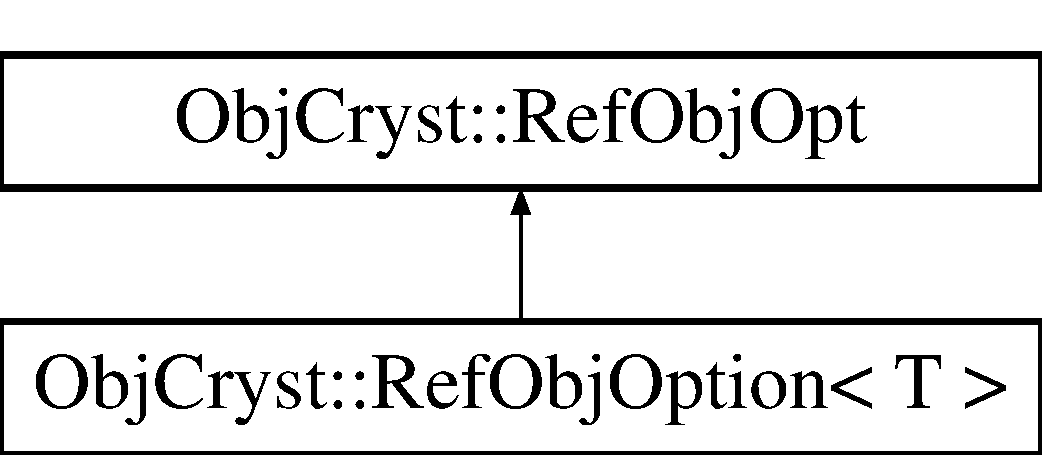
\includegraphics[height=4cm]{a00084}
\end{center}
\end{figure}
\subsubsection*{Public Member Functions}
\begin{DoxyCompactItemize}
\item 
{\bf Scatterer} ()\label{a00084_a5367833f94dd2daeed41ffe3836c1c64}

\begin{DoxyCompactList}\small\item\em Constructor. \item\end{DoxyCompactList}\item 
{\bf Scatterer} (const {\bf Scatterer} \&old)\label{a00084_a0d568f50de46100c0faff213dde8544f}

\begin{DoxyCompactList}\small\item\em Copy Constructor. \item\end{DoxyCompactList}\item 
virtual {\bf $\sim$Scatterer} ()\label{a00084_a5e28b2aa0b7f8e82b533bb8aec288b21}

\begin{DoxyCompactList}\small\item\em Destructor. \item\end{DoxyCompactList}\item 
virtual {\bf Scatterer} $\ast$ {\bf CreateCopy} () const =0
\item 
virtual const string \& {\bf GetClassName} () const 
\begin{DoxyCompactList}\small\item\em Name for this class (\char`\"{}RefinableObj\char`\"{}, \char`\"{}Crystal\char`\"{},. \item\end{DoxyCompactList}\item 
virtual int {\bf GetNbComponent} () const =0\label{a00084_a18d63b8e79b35942902244c555ea33ef}

\begin{DoxyCompactList}\small\item\em Number of components in the scatterer (eg number of point scatterers). \item\end{DoxyCompactList}\item 
virtual const {\bf ScatteringComponentList} \& {\bf GetScatteringComponentList} () const =0
\begin{DoxyCompactList}\small\item\em Get the list of all scattering components for this scatterer. \item\end{DoxyCompactList}\item 
virtual string {\bf GetComponentName} (const int i) const =0
\begin{DoxyCompactList}\small\item\em Name for the i-\/th component of this scatterer. \item\end{DoxyCompactList}\item 
REAL {\bf GetX} () const 
\begin{DoxyCompactList}\small\item\em X coordinate (fractionnal) of the scatterer (for complex scatterers, this corresponds to the position of one atom of the \doxyref{Scatterer}{p.}{a00084}, ideally it should be near the center of the \doxyref{Scatterer}{p.}{a00084}. \item\end{DoxyCompactList}\item 
REAL {\bf GetY} () const 
\begin{DoxyCompactList}\small\item\em Y coordinate (fractionnal) of the scatterer (for complex scatterers, this corresponds to the position of one atom of the \doxyref{Scatterer}{p.}{a00084}, ideally it should be near the center of the \doxyref{Scatterer}{p.}{a00084}. \item\end{DoxyCompactList}\item 
REAL {\bf GetZ} () const 
\begin{DoxyCompactList}\small\item\em Z coordinate (fractionnal) of the scatterer (for complex scatterers, this corresponds to the position of one atom of the \doxyref{Scatterer}{p.}{a00084}, ideally it should be near the center of the \doxyref{Scatterer}{p.}{a00084}. \item\end{DoxyCompactList}\item 
REAL {\bf GetOccupancy} () const 
\begin{DoxyCompactList}\small\item\em Get the occupancy of the scatterer (0. \item\end{DoxyCompactList}\item 
virtual void {\bf SetX} (const REAL x)
\begin{DoxyCompactList}\small\item\em X coordinate (fractionnal) of the scatterer (for complex scatterers, this corresponds to the position of one atom of the \doxyref{Scatterer}{p.}{a00084}, ideally it should be near the center of the \doxyref{Scatterer}{p.}{a00084}. \item\end{DoxyCompactList}\item 
virtual void {\bf SetY} (const REAL y)
\begin{DoxyCompactList}\small\item\em Y coordinate (fractionnal) of the scatterer (for complex scatterers, this corresponds to the position of one atom of the \doxyref{Scatterer}{p.}{a00084}, ideally it should be near the center of the \doxyref{Scatterer}{p.}{a00084}. \item\end{DoxyCompactList}\item 
virtual void {\bf SetZ} (const REAL z)
\begin{DoxyCompactList}\small\item\em Z coordinate (fractionnal) of the scatterer (for complex scatterers, this corresponds to the position of one atom of the \doxyref{Scatterer}{p.}{a00084}, ideally it should be near the center of the \doxyref{Scatterer}{p.}{a00084}. \item\end{DoxyCompactList}\item 
virtual void {\bf SetOccupancy} (const REAL occupancy)
\begin{DoxyCompactList}\small\item\em Change the occupancy of the scatterer (0. \item\end{DoxyCompactList}\item 
{\bf operator string} () const 
\begin{DoxyCompactList}\small\item\em Conversion function. \item\end{DoxyCompactList}\item 
virtual void {\bf Print} () const =0\label{a00084_a0d865e9598c10ce4db5ff8885ecbc0a9}

\begin{DoxyCompactList}\small\item\em Print some info about the scatterer (ideally this should be one line...). \item\end{DoxyCompactList}\item 
virtual const string \& {\bf GetColour} () const 
\begin{DoxyCompactList}\small\item\em Colour associated to this scatterer (using POVRay names). \item\end{DoxyCompactList}\item 
virtual const float $\ast$ {\bf GetColourRGB} () const \label{a00084_ae79467fc8546f90dc51a42037a8d193e}

\begin{DoxyCompactList}\small\item\em Colour associated to this scatterer, 3 RGB Coordinates. \item\end{DoxyCompactList}\item 
virtual ostream \& {\bf POVRayDescription} (ostream \&os, const {\bf CrystalPOVRayOptions} \&options) const =0
\item 
virtual void {\bf GLInitDisplayList} (const bool noSymmetrics=false, const REAL xMin=-\/.1, const REAL xMax=1.1, const REAL yMin=-\/.1, const REAL yMax=1.1, const REAL zMin=-\/.1, const REAL zMax=1.1, const bool displayEnantiomer=false, const bool displayNames=false) const =0
\item 
const {\bf RefinableObjClock} \& {\bf GetClockScatterer} () const \label{a00084_a9f72e14ca11568fc85bb808b720883fc}

\begin{DoxyCompactList}\small\item\em Last time anything in the scatterer was changed (atoms, positions, scattering power). \item\end{DoxyCompactList}\item 
{\bf RefinableObjClock} \& {\bf GetClockScatterer} ()\label{a00084_a02f9ce5c724e92ca8eb7c6e4322f8c85}

\begin{DoxyCompactList}\small\item\em Last time anything in the scatterer was changed (atoms, positions, scattering power). \item\end{DoxyCompactList}\item 
void {\bf SetCrystal} ({\bf Crystal} \&)\label{a00084_ace072c5113b5328a7145d33779582621}

\begin{DoxyCompactList}\small\item\em Set the crystal in which is included this \doxyref{Scatterer}{p.}{a00084}. \item\end{DoxyCompactList}\item 
const {\bf Crystal} \& {\bf GetCrystal} () const \label{a00084_a89eed8d88f9e3f31957353254b9bbc81}

\begin{DoxyCompactList}\small\item\em In which crystal is this \doxyref{Scatterer}{p.}{a00084} included ? \item\end{DoxyCompactList}\item 
{\bf Crystal} \& {\bf GetCrystal} ()\label{a00084_acc71fa0e4198adc72c64480628e5e49c}

\begin{DoxyCompactList}\small\item\em In which crystal is this \doxyref{Scatterer}{p.}{a00084} included ? \item\end{DoxyCompactList}\end{DoxyCompactItemize}
\subsubsection*{Protected Member Functions}
\begin{DoxyCompactItemize}
\item 
virtual void {\bf InitRefParList} ()=0
\item 
virtual void {\bf InitRGBColour} ()
\begin{DoxyCompactList}\small\item\em Get RGB Colour coordinates from Colour Name. \item\end{DoxyCompactList}\item 
const {\bf RefinableObjClock} \& {\bf GetClockScattCompList} () const \label{a00084_a204e5b5ba54b967074c6de965940b00e}

\begin{DoxyCompactList}\small\item\em Last time the \doxyref{ScatteringComponentList}{p.}{a00086} was generated. \item\end{DoxyCompactList}\end{DoxyCompactItemize}
\subsubsection*{Protected Attributes}
\begin{DoxyCompactItemize}
\item 
CrystVector\_\-REAL {\bf mXYZ}\label{a00084_a9cc523b07c82846bf0ddc3ce0e74bcc6}

\begin{DoxyCompactList}\small\item\em coordinates of the scatterer (or of its center..) \item\end{DoxyCompactList}\item 
REAL {\bf mOccupancy}
\begin{DoxyCompactList}\small\item\em Occupancy : 0 $<$= occ $<$= 1 For a multi-\/atom scatterer (polyhedron,. \item\end{DoxyCompactList}\item 
string {\bf mColourName}\label{a00084_a1d1166aabc3a811ca70e37d2ad03ba05}

\begin{DoxyCompactList}\small\item\em Colour for this scatterer (from POVRay). \item\end{DoxyCompactList}\item 
float {\bf mColourRGB} [3]\label{a00084_ab62464d3d132a8e70f283648ae9ea020}

\begin{DoxyCompactList}\small\item\em Colour for this scatterer using RGB. \item\end{DoxyCompactList}\item 
{\bf RefinableObjClock} {\bf mClockScatterer}\label{a00084_ace0238cbbd28dd0adb9e6102bc2b8cae}

\begin{DoxyCompactList}\small\item\em Last time anything (number of atoms, positions, scattering power) was changed. \item\end{DoxyCompactList}\item 
{\bf RefinableObjClock} {\bf mClockScattCompList}
\item 
{\bf Crystal} $\ast$ {\bf mpCryst}
\begin{DoxyCompactList}\small\item\em The crystal in which the \doxyref{Scatterer}{p.}{a00084} is This is needed so that we can know which scattering powers are available in the crystal, and also to convert fractionnal to orthonormal coordinates (for some scatterers only). \item\end{DoxyCompactList}\end{DoxyCompactItemize}


\subsubsection{Detailed Description}
Generic type of scatterer: can be an atom, or a more complex assembly of atoms. A \doxyref{Scatterer}{p.}{a00084} is able to give its position (in fractionnal coordinates) in the unit cell, and more generally the position of all point scattering centers (\doxyref{ScatteringComponent}{p.}{a00085}), along with the \doxyref{ScatteringPower}{p.}{a00089} associated with each position.

For simple atoms, there is only one scattering position with the associated scattering power (scattering factor, anomalous, thermic). For complex scatterers (molecules: \doxyref{ZScatterer}{p.}{a00155}) there are as many positions as atoms.

A scatterer also has a few functions to display itself in 3D

This is an abstract base class. 

\subsubsection{Member Function Documentation}
\index{ObjCryst::Scatterer@{ObjCryst::Scatterer}!CreateCopy@{CreateCopy}}
\index{CreateCopy@{CreateCopy}!ObjCryst::Scatterer@{ObjCryst::Scatterer}}
\paragraph[{CreateCopy}]{\setlength{\rightskip}{0pt plus 5cm}virtual {\bf Scatterer}$\ast$ ObjCryst::Scatterer::CreateCopy () const\hspace{0.3cm}{\ttfamily  [pure virtual]}}\hfill\label{a00084_a4d374adcff97163a24492d362f6def73}
\begin{DoxyInternal}{For internal use only.}
so-\/called Virtual copy constructor, needed to make copies of arrays of Scatterers \end{DoxyInternal}


Implemented in {\bf ObjCryst::Atom} \doxyref{}{p.}{a00008_af5215404ae1f180ed84046700845f92a}, {\bf ObjCryst::Molecule} \doxyref{}{p.}{a00046_a96728865d25881151b7010d3eaf4ec0f}, {\bf ObjCryst::ZScatterer} \doxyref{}{p.}{a00155_a6cf9f5891cf87e865efa971d36599d24}, and {\bf ObjCryst::ZPolyhedron} \doxyref{}{p.}{a00154_a83436a907a22d794259e5fea9b7670ce}.\index{ObjCryst::Scatterer@{ObjCryst::Scatterer}!GetClassName@{GetClassName}}
\index{GetClassName@{GetClassName}!ObjCryst::Scatterer@{ObjCryst::Scatterer}}
\paragraph[{GetClassName}]{\setlength{\rightskip}{0pt plus 5cm}virtual const string\& ObjCryst::Scatterer::GetClassName () const\hspace{0.3cm}{\ttfamily  [virtual]}}\hfill\label{a00084_a374fc1bb2887ab1f61d456326d97c05f}


Name for this class (\char`\"{}RefinableObj\char`\"{}, \char`\"{}Crystal\char`\"{},. ..). This is only useful to distinguish different classes when picking up objects from the \doxyref{RefinableObj}{p.}{a00070} Global Registry 

Reimplemented from {\bf ObjCryst::RefinableObj} \doxyref{}{p.}{a00070_a62968d90a7a3080738b363934616c019}.

Reimplemented in {\bf ObjCryst::Atom} \doxyref{}{p.}{a00008_a9f0d1cb7c3b1db1baf84076e5da0ca0e}, {\bf ObjCryst::Molecule} \doxyref{}{p.}{a00046_a7f0f1ae6670032f5afc9ccf65d45f8c4}, and {\bf ObjCryst::ZScatterer} \doxyref{}{p.}{a00155_a610a62c221ed289e1ce4d68adac921ee}.\index{ObjCryst::Scatterer@{ObjCryst::Scatterer}!GetColour@{GetColour}}
\index{GetColour@{GetColour}!ObjCryst::Scatterer@{ObjCryst::Scatterer}}
\paragraph[{GetColour}]{\setlength{\rightskip}{0pt plus 5cm}virtual const string\& ObjCryst::Scatterer::GetColour () const\hspace{0.3cm}{\ttfamily  [virtual]}}\hfill\label{a00084_a2db9df8f429181af0e478ba74c16cb27}


Colour associated to this scatterer (using POVRay names). \index{ObjCryst::Scatterer@{ObjCryst::Scatterer}!GetComponentName@{GetComponentName}}
\index{GetComponentName@{GetComponentName}!ObjCryst::Scatterer@{ObjCryst::Scatterer}}
\paragraph[{GetComponentName}]{\setlength{\rightskip}{0pt plus 5cm}virtual string ObjCryst::Scatterer::GetComponentName (const int {\em i}) const\hspace{0.3cm}{\ttfamily  [pure virtual]}}\hfill\label{a00084_a42bdf508da6a90859a5a61e16c27d47e}


Name for the i-\/th component of this scatterer. If the component is an \doxyref{Atom}{p.}{a00008}, Then the name is that of the atom. Else, it is the name of the scatterer plus the component number in the scatterer plus the name of the \doxyref{ScatteringPower}{p.}{a00089}. \begin{DoxyNote}{Note}
It would be better to return a reference, but we don't want to keep a name for all components... Weeelll, needs some more thinking... see what performance hit results (if any).
\end{DoxyNote}
\begin{Desc}
\item[{\bf Bug}]does not take into account dummy atoms !! \end{Desc}


Implemented in {\bf ObjCryst::Atom} \doxyref{}{p.}{a00008_a88fed92945210af0e6cf28e34fa545f4}, {\bf ObjCryst::Molecule} \doxyref{}{p.}{a00046_a8dae19447740afaa1780e39a61f625c9}, and {\bf ObjCryst::ZScatterer} \doxyref{}{p.}{a00155_a44e9bf9d72e256ef8bc39ea2cf0eef4e}.\index{ObjCryst::Scatterer@{ObjCryst::Scatterer}!GetOccupancy@{GetOccupancy}}
\index{GetOccupancy@{GetOccupancy}!ObjCryst::Scatterer@{ObjCryst::Scatterer}}
\paragraph[{GetOccupancy}]{\setlength{\rightskip}{0pt plus 5cm}REAL ObjCryst::Scatterer::GetOccupancy () const}\hfill\label{a00084_a11c4a95b3299bf8cbdc29ceea5815aad}


Get the occupancy of the scatterer (0. -\/$>$ 1.0)

The occupancy is given in \%, and must take into account the 'special position' character of atoms (ie an atom on a 2fold axis should have at most a .5 population, etc...). For a multi-\/atom scatterer (polyhedra), this is the {\bfseries overall} occupancy of the scatterer, affecting all atoms. \index{ObjCryst::Scatterer@{ObjCryst::Scatterer}!GetScatteringComponentList@{GetScatteringComponentList}}
\index{GetScatteringComponentList@{GetScatteringComponentList}!ObjCryst::Scatterer@{ObjCryst::Scatterer}}
\paragraph[{GetScatteringComponentList}]{\setlength{\rightskip}{0pt plus 5cm}virtual const {\bf ScatteringComponentList}\& ObjCryst::Scatterer::GetScatteringComponentList () const\hspace{0.3cm}{\ttfamily  [pure virtual]}}\hfill\label{a00084_aca0e08e3793cc69d31fce53e481c2a67}


Get the list of all scattering components for this scatterer. This is the most important function of this class, giving the list of scattering positions along with the associated \doxyref{ScatteringPower}{p.}{a00089}. 

Implemented in {\bf ObjCryst::Atom} \doxyref{}{p.}{a00008_a3483660b1d08b113af61d708ecff8d1a}, {\bf ObjCryst::Molecule} \doxyref{}{p.}{a00046_a3ac17bd45a709c82d9a4d304fde09b88}, and {\bf ObjCryst::ZScatterer} \doxyref{}{p.}{a00155_aadfeeafb618aad01ea80f099dd7c3299}.\index{ObjCryst::Scatterer@{ObjCryst::Scatterer}!GetX@{GetX}}
\index{GetX@{GetX}!ObjCryst::Scatterer@{ObjCryst::Scatterer}}
\paragraph[{GetX}]{\setlength{\rightskip}{0pt plus 5cm}REAL ObjCryst::Scatterer::GetX () const}\hfill\label{a00084_a36051907538dc50c4989fcbff5b9d4e6}


X coordinate (fractionnal) of the scatterer (for complex scatterers, this corresponds to the position of one atom of the \doxyref{Scatterer}{p.}{a00084}, ideally it should be near the center of the \doxyref{Scatterer}{p.}{a00084}. \index{ObjCryst::Scatterer@{ObjCryst::Scatterer}!GetY@{GetY}}
\index{GetY@{GetY}!ObjCryst::Scatterer@{ObjCryst::Scatterer}}
\paragraph[{GetY}]{\setlength{\rightskip}{0pt plus 5cm}REAL ObjCryst::Scatterer::GetY () const}\hfill\label{a00084_afd11a010b62690b84dacea7e47176ec1}


Y coordinate (fractionnal) of the scatterer (for complex scatterers, this corresponds to the position of one atom of the \doxyref{Scatterer}{p.}{a00084}, ideally it should be near the center of the \doxyref{Scatterer}{p.}{a00084}. \index{ObjCryst::Scatterer@{ObjCryst::Scatterer}!GetZ@{GetZ}}
\index{GetZ@{GetZ}!ObjCryst::Scatterer@{ObjCryst::Scatterer}}
\paragraph[{GetZ}]{\setlength{\rightskip}{0pt plus 5cm}REAL ObjCryst::Scatterer::GetZ () const}\hfill\label{a00084_a667e97f3e177bc74dfc3cbd582afaad5}


Z coordinate (fractionnal) of the scatterer (for complex scatterers, this corresponds to the position of one atom of the \doxyref{Scatterer}{p.}{a00084}, ideally it should be near the center of the \doxyref{Scatterer}{p.}{a00084}. \index{ObjCryst::Scatterer@{ObjCryst::Scatterer}!GLInitDisplayList@{GLInitDisplayList}}
\index{GLInitDisplayList@{GLInitDisplayList}!ObjCryst::Scatterer@{ObjCryst::Scatterer}}
\paragraph[{GLInitDisplayList}]{\setlength{\rightskip}{0pt plus 5cm}virtual void ObjCryst::Scatterer::GLInitDisplayList (const bool {\em noSymmetrics} = {\ttfamily false}, \/  const REAL {\em xMin} = {\ttfamily -\/.1}, \/  const REAL {\em xMax} = {\ttfamily 1.1}, \/  const REAL {\em yMin} = {\ttfamily -\/.1}, \/  const REAL {\em yMax} = {\ttfamily 1.1}, \/  const REAL {\em zMin} = {\ttfamily -\/.1}, \/  const REAL {\em zMax} = {\ttfamily 1.1}, \/  const bool {\em displayEnantiomer} = {\ttfamily false}, \/  const bool {\em displayNames} = {\ttfamily false}) const\hspace{0.3cm}{\ttfamily  [pure virtual]}}\hfill\label{a00084_a4eaf9cf9780bef83e40155810db120a0}
\begin{DoxyInternal}{For internal use only.}
Create an OpenGL Display List of the scatterer. This should only be called by a \doxyref{Crystal}{p.}{a00020} object.


\begin{DoxyParams}{Parameters}
\item[{\em noSymmetrics,:}]if false (the default), then all symmetrics are shown in the 3D display, within the limits defined by the min/max parameters $\backslash$ param xMin,xMax,yMin,yMax,zMin,zMax: in fractionnal coordinates, the region in which we want scaterrer to be displayed. The test is made on the center of the scatterer (eg a \doxyref{ZScatterer}{p.}{a00155} (molecule) will not be 'cut' on the border). \item[{\em displayNames,:}]if true, only the names of the scatterers will be displayed, at the position of the scatterers (to actually see them, they will have to be translated with respect to the drawing of the scatterers). \end{DoxyParams}
\end{DoxyInternal}


Implemented in {\bf ObjCryst::Atom} \doxyref{}{p.}{a00008_a14e239415f6923d83ceff1347b89393b}, {\bf ObjCryst::Molecule} \doxyref{}{p.}{a00046_a00aa7620326d8663b1f4e1bd9237ffb8}, and {\bf ObjCryst::ZScatterer} \doxyref{}{p.}{a00155_a17fb665a72c2d694410580e3b33ea1a9}.\index{ObjCryst::Scatterer@{ObjCryst::Scatterer}!InitRefParList@{InitRefParList}}
\index{InitRefParList@{InitRefParList}!ObjCryst::Scatterer@{ObjCryst::Scatterer}}
\paragraph[{InitRefParList}]{\setlength{\rightskip}{0pt plus 5cm}virtual void ObjCryst::Scatterer::InitRefParList ()\hspace{0.3cm}{\ttfamily  [protected, pure virtual]}}\hfill\label{a00084_a45ef328b68a0a68c0228beefc25cda7f}
\begin{DoxyInternal}{For internal use only.}
Prepare refinable parameters for the scatterer object \end{DoxyInternal}


Implemented in {\bf ObjCryst::Atom} \doxyref{}{p.}{a00008_a72fe4868d70c8068483ba635029bbc86}, {\bf ObjCryst::Molecule} \doxyref{}{p.}{a00046_ad96fe78688ce898dc9aeffcc23523967}, and {\bf ObjCryst::ZScatterer} \doxyref{}{p.}{a00155_a36839536bcb14d3a8dd581baf168f3d7}.\index{ObjCryst::Scatterer@{ObjCryst::Scatterer}!InitRGBColour@{InitRGBColour}}
\index{InitRGBColour@{InitRGBColour}!ObjCryst::Scatterer@{ObjCryst::Scatterer}}
\paragraph[{InitRGBColour}]{\setlength{\rightskip}{0pt plus 5cm}virtual void ObjCryst::Scatterer::InitRGBColour ()\hspace{0.3cm}{\ttfamily  [protected, virtual]}}\hfill\label{a00084_a0142f5a84db948319c3ff310315c8599}


Get RGB Colour coordinates from Colour Name. Note that the colour used for display is usually that of the \doxyref{ScatteringPower}{p.}{a00089}, not that of the \doxyref{Scatterer}{p.}{a00084} \index{ObjCryst::Scatterer@{ObjCryst::Scatterer}!operator string@{operator string}}
\index{operator string@{operator string}!ObjCryst::Scatterer@{ObjCryst::Scatterer}}
\paragraph[{operator string}]{\setlength{\rightskip}{0pt plus 5cm}ObjCryst::Scatterer::operator string () const}\hfill\label{a00084_a121e6e739f9b740564afc32c8c74a664}


Conversion function. -\/$>$ returns the scatt name

\begin{DoxyWarning}{Warning}
EXPERIMENTAL. DO NOT USE, as this may be removed. 
\end{DoxyWarning}
\index{ObjCryst::Scatterer@{ObjCryst::Scatterer}!POVRayDescription@{POVRayDescription}}
\index{POVRayDescription@{POVRayDescription}!ObjCryst::Scatterer@{ObjCryst::Scatterer}}
\paragraph[{POVRayDescription}]{\setlength{\rightskip}{0pt plus 5cm}virtual ostream\& ObjCryst::Scatterer::POVRayDescription (ostream \& {\em os}, \/  const {\bf CrystalPOVRayOptions} \& {\em options}) const\hspace{0.3cm}{\ttfamily  [pure virtual]}}\hfill\label{a00084_a708cc857f82c9af4cbdf4d9334449d0f}
\begin{DoxyInternal}{For internal use only.}
Output a description of the scatterer for POVRay. This should only be called by the \doxyref{Crystal}{p.}{a00020} Object to which belongs this scatterer. \end{DoxyInternal}


Implemented in {\bf ObjCryst::Atom} \doxyref{}{p.}{a00008_a2994321bc2974d853f36b011d23a94b3}, {\bf ObjCryst::Molecule} \doxyref{}{p.}{a00046_a98bd83a14b359c994be9ab1bf4b8453b}, and {\bf ObjCryst::ZScatterer} \doxyref{}{p.}{a00155_a6dd20fe536310e622c1a30fb1d5a788f}.\index{ObjCryst::Scatterer@{ObjCryst::Scatterer}!SetOccupancy@{SetOccupancy}}
\index{SetOccupancy@{SetOccupancy}!ObjCryst::Scatterer@{ObjCryst::Scatterer}}
\paragraph[{SetOccupancy}]{\setlength{\rightskip}{0pt plus 5cm}virtual void ObjCryst::Scatterer::SetOccupancy (const REAL {\em occupancy})\hspace{0.3cm}{\ttfamily  [virtual]}}\hfill\label{a00084_a43c371cd475f921e94c6a13b7c1d89a0}


Change the occupancy of the scatterer (0. -\/$>$ 1.0)

The occupancy is given in \%, and must take into account the 'special position' character of atoms (ie an atom on a 2fold axis should have at most a .5 population, etc...). For a multi-\/atom scatterer (polyhedra), this is the {\bfseries overall} occupancy of the scatterer, affecting all atoms. \index{ObjCryst::Scatterer@{ObjCryst::Scatterer}!SetX@{SetX}}
\index{SetX@{SetX}!ObjCryst::Scatterer@{ObjCryst::Scatterer}}
\paragraph[{SetX}]{\setlength{\rightskip}{0pt plus 5cm}virtual void ObjCryst::Scatterer::SetX (const REAL {\em x})\hspace{0.3cm}{\ttfamily  [virtual]}}\hfill\label{a00084_aaefba31ab4187b0f826436929f3c0456}


X coordinate (fractionnal) of the scatterer (for complex scatterers, this corresponds to the position of one atom of the \doxyref{Scatterer}{p.}{a00084}, ideally it should be near the center of the \doxyref{Scatterer}{p.}{a00084}. \index{ObjCryst::Scatterer@{ObjCryst::Scatterer}!SetY@{SetY}}
\index{SetY@{SetY}!ObjCryst::Scatterer@{ObjCryst::Scatterer}}
\paragraph[{SetY}]{\setlength{\rightskip}{0pt plus 5cm}virtual void ObjCryst::Scatterer::SetY (const REAL {\em y})\hspace{0.3cm}{\ttfamily  [virtual]}}\hfill\label{a00084_afeaa60aaa33907fb6d974f626d91a390}


Y coordinate (fractionnal) of the scatterer (for complex scatterers, this corresponds to the position of one atom of the \doxyref{Scatterer}{p.}{a00084}, ideally it should be near the center of the \doxyref{Scatterer}{p.}{a00084}. \index{ObjCryst::Scatterer@{ObjCryst::Scatterer}!SetZ@{SetZ}}
\index{SetZ@{SetZ}!ObjCryst::Scatterer@{ObjCryst::Scatterer}}
\paragraph[{SetZ}]{\setlength{\rightskip}{0pt plus 5cm}virtual void ObjCryst::Scatterer::SetZ (const REAL {\em z})\hspace{0.3cm}{\ttfamily  [virtual]}}\hfill\label{a00084_ab7bd1b921a51b476ee776624425ac46c}


Z coordinate (fractionnal) of the scatterer (for complex scatterers, this corresponds to the position of one atom of the \doxyref{Scatterer}{p.}{a00084}, ideally it should be near the center of the \doxyref{Scatterer}{p.}{a00084}. 

\subsubsection{Member Data Documentation}
\index{ObjCryst::Scatterer@{ObjCryst::Scatterer}!mClockScattCompList@{mClockScattCompList}}
\index{mClockScattCompList@{mClockScattCompList}!ObjCryst::Scatterer@{ObjCryst::Scatterer}}
\paragraph[{mClockScattCompList}]{\setlength{\rightskip}{0pt plus 5cm}{\bf RefinableObjClock} {\bf ObjCryst::Scatterer::mClockScattCompList}\hspace{0.3cm}{\ttfamily  [mutable, protected]}}\hfill\label{a00084_a807f373561fbd1c460b0dfc40924e542}
\begin{DoxyInternal}{For internal use only.}
Last time the \doxyref{ScatteringComponentList}{p.}{a00086} was generated \end{DoxyInternal}
\index{ObjCryst::Scatterer@{ObjCryst::Scatterer}!mOccupancy@{mOccupancy}}
\index{mOccupancy@{mOccupancy}!ObjCryst::Scatterer@{ObjCryst::Scatterer}}
\paragraph[{mOccupancy}]{\setlength{\rightskip}{0pt plus 5cm}REAL {\bf ObjCryst::Scatterer::mOccupancy}\hspace{0.3cm}{\ttfamily  [protected]}}\hfill\label{a00084_ae51b357e1cf9f523994f0e08c70bb489}


Occupancy : 0 $<$= occ $<$= 1 For a multi-\/atom scatterer (polyhedron,. .), this is the {\bfseries overall} occupancy of the scatterer (affects all components of the scatterer). \index{ObjCryst::Scatterer@{ObjCryst::Scatterer}!mpCryst@{mpCryst}}
\index{mpCryst@{mpCryst}!ObjCryst::Scatterer@{ObjCryst::Scatterer}}
\paragraph[{mpCryst}]{\setlength{\rightskip}{0pt plus 5cm}{\bf Crystal}$\ast$ {\bf ObjCryst::Scatterer::mpCryst}\hspace{0.3cm}{\ttfamily  [protected]}}\hfill\label{a00084_a359e6115a710c44bf340f439a17cb073}


The crystal in which the \doxyref{Scatterer}{p.}{a00084} is This is needed so that we can know which scattering powers are available in the crystal, and also to convert fractionnal to orthonormal coordinates (for some scatterers only). It cannot be const since some scatterers may want to modify the list of scattering powers of the crystal... 

The documentation for this class was generated from the following file:\begin{DoxyCompactItemize}
\item 
Scatterer.h\end{DoxyCompactItemize}

\subsection{ObjCryst::ScatteringComponent Struct Reference}
\label{a00085}\index{ObjCryst::ScatteringComponent@{ObjCryst::ScatteringComponent}}


A scattering position in a crystal, associated with the corresponding occupancy and a pointer to the \doxyref{ScatteringPower}{p.}{a00089}.  
\subsubsection*{Public Member Functions}
\begin{DoxyCompactItemize}
\item 
bool {\bfseries operator==} (const {\bf ScatteringComponent} \&rhs) const \label{a00085_a3c90ac5f4f15fd8ab4e1272a542ce4a9}

\item 
bool {\bfseries operator!=} (const {\bf ScatteringComponent} \&rhs) const \label{a00085_a7a2f4b968cc15b1adbfb0dda7e8b3452}

\item 
void {\bf Print} () const \label{a00085_ae539b046ae25fba220ef58881c2fe9b7}

\begin{DoxyCompactList}\small\item\em Print one line oabout this component. \item\end{DoxyCompactList}\end{DoxyCompactItemize}
\subsubsection*{Public Attributes}
\begin{DoxyCompactItemize}
\item 
REAL {\bf mX}\label{a00085_a5e298bbfa80dc72cbf666bd8007c1a58}

\begin{DoxyCompactList}\small\item\em Coordinates of scattering positions i the crystal with the corresponding occupancy. \item\end{DoxyCompactList}\item 
REAL {\bfseries mY}\label{a00085_a0ad9f5614c3240d3b97310da61180a48}

\item 
REAL {\bfseries mZ}\label{a00085_a6e3cf2fb825a1a6912bf9cebc62d4cf7}

\item 
REAL {\bfseries mOccupancy}\label{a00085_a845b921b1d5945619b5bfcb87264c125}

\item 
const {\bf ScatteringPower} $\ast$ {\bf mpScattPow}\label{a00085_a1aa0c754e20ac3a0489ed57c0cb31bd3}

\begin{DoxyCompactList}\small\item\em The \doxyref{ScatteringPower}{p.}{a00089} associated with this position. \item\end{DoxyCompactList}\item 
REAL {\bf mDynPopCorr}
\begin{DoxyCompactList}\small\item\em Dynamical Population Correction. \item\end{DoxyCompactList}\end{DoxyCompactItemize}


\subsubsection{Detailed Description}
A scattering position in a crystal, associated with the corresponding occupancy and a pointer to the \doxyref{ScatteringPower}{p.}{a00089}. Also given is the 

\subsubsection{Member Data Documentation}
\index{ObjCryst::ScatteringComponent@{ObjCryst::ScatteringComponent}!mDynPopCorr@{mDynPopCorr}}
\index{mDynPopCorr@{mDynPopCorr}!ObjCryst::ScatteringComponent@{ObjCryst::ScatteringComponent}}
\paragraph[{mDynPopCorr}]{\setlength{\rightskip}{0pt plus 5cm}REAL {\bf ObjCryst::ScatteringComponent::mDynPopCorr}\hspace{0.3cm}{\ttfamily  [mutable]}}\hfill\label{a00085_a33af12bb3f340af259a8b8450f837efd}


Dynamical Population Correction. The population of any atom is given by mOccupancy$\ast$mDynPopCorr. mPopu is the {\itshape real\/} mOccupancy (0$<$.$<$1), and should be the only one used during a refinement. However during a {\itshape model\/} {\itshape search\/} for the structure, atoms may fall unexpectedly in a special position or with an overlap of two atoms (the shared oxygen between two polyhedras, for example). In these cases it is necessary to dynamically correct the population during the generation of structural models. See also \doxyref{Crystal::CalcDynPopCorr}{p.}{a00020_a69975008974c9603ebb794bb6bb20fe8}

\begin{DoxyNote}{Note}
this parameter is mutable, and is computed by the \doxyref{Crystal}{p.}{a00020} object 
\end{DoxyNote}


The documentation for this struct was generated from the following file:\begin{DoxyCompactItemize}
\item 
ScatteringPower.h\end{DoxyCompactItemize}

\subsection{Obj\-Cryst\-:\-:Ref\-Obj\-Option$<$ T $>$ Class Template Reference}
\label{a00086}\index{Obj\-Cryst\-::\-Ref\-Obj\-Option$<$ T $>$@{Obj\-Cryst\-::\-Ref\-Obj\-Option$<$ T $>$}}


Class for options of \doxyref{Refinable\-Obj}{p.}{a00078}, templated so that we can warn the object that something has been changed.  


Inheritance diagram for Obj\-Cryst\-:\-:Ref\-Obj\-Option$<$ T $>$\-:\begin{figure}[H]
\begin{center}
\leavevmode
\includegraphics[height=2.000000cm]{a00086}
\end{center}
\end{figure}
\subsubsection*{Public Member Functions}
\begin{DoxyCompactItemize}
\item 
{\bf Ref\-Obj\-Option} (T $\ast$obj)
\begin{DoxyCompactList}\small\item\em Constructor for the option. \end{DoxyCompactList}\item 
void {\bfseries Init} (const int nb\-Choice, const string $\ast$name, const string $\ast$choice\-Names, void(T\-::$\ast$fp)(const int))\label{a00086_a8369dfcf480e3d788f2ec097a161ab9b}

\item 
virtual void {\bfseries Set\-Choice} (const int choice)\label{a00086_ac4d0be41e98e1b65b22673203e6c9495}

\end{DoxyCompactItemize}
\subsubsection*{Private Attributes}
\begin{DoxyCompactItemize}
\item 
T $\ast$ {\bf mp\-Obj}\label{a00086_a76e1fae7a6f442c05aed8aa0f0f2fb05}

\begin{DoxyCompactList}\small\item\em The object which uses this option. \end{DoxyCompactList}\item 
void(T\-::$\ast$ {\bf mfp\-Set\-New\-Value} )(const int)
\begin{DoxyCompactList}\small\item\em The pointer to the member function to be used when the choice is changed, to notify immediately the object. \end{DoxyCompactList}\end{DoxyCompactItemize}
\subsubsection*{Additional Inherited Members}


\subsubsection{Detailed Description}
\subsubsection*{template$<$class T$>$class Obj\-Cryst\-::\-Ref\-Obj\-Option$<$ T $>$}

Class for options of \doxyref{Refinable\-Obj}{p.}{a00078}, templated so that we can warn the object that something has been changed. 

N\-O\-T U\-S\-E\-D S\-O F\-A\-R. 

\subsubsection{Constructor \& Destructor Documentation}
\index{Obj\-Cryst\-::\-Ref\-Obj\-Option@{Obj\-Cryst\-::\-Ref\-Obj\-Option}!Ref\-Obj\-Option@{Ref\-Obj\-Option}}
\index{Ref\-Obj\-Option@{Ref\-Obj\-Option}!ObjCryst::RefObjOption@{Obj\-Cryst\-::\-Ref\-Obj\-Option}}
\paragraph[{Ref\-Obj\-Option}]{\setlength{\rightskip}{0pt plus 5cm}template$<$class T $>$ {\bf Obj\-Cryst\-::\-Ref\-Obj\-Option}$<$ T $>$\-::{\bf Ref\-Obj\-Option} (
\begin{DoxyParamCaption}
\item[{T $\ast$}]{obj}
\end{DoxyParamCaption}
)}\label{a00086_a501cc1ee9602c16d9ccbda004ddae5c3}


Constructor for the option. 


\begin{DoxyParams}{Parameters}
{\em obj,\-:} & the \\
\hline
\end{DoxyParams}


\subsubsection{Member Data Documentation}
\index{Obj\-Cryst\-::\-Ref\-Obj\-Option@{Obj\-Cryst\-::\-Ref\-Obj\-Option}!mfp\-Set\-New\-Value@{mfp\-Set\-New\-Value}}
\index{mfp\-Set\-New\-Value@{mfp\-Set\-New\-Value}!ObjCryst::RefObjOption@{Obj\-Cryst\-::\-Ref\-Obj\-Option}}
\paragraph[{mfp\-Set\-New\-Value}]{\setlength{\rightskip}{0pt plus 5cm}template$<$class T $>$ void(T\-::$\ast$ {\bf Obj\-Cryst\-::\-Ref\-Obj\-Option}$<$ T $>$\-::mfp\-Set\-New\-Value)(const int)\hspace{0.3cm}{\ttfamily [private]}}\label{a00086_a460ca91a71b4083e29ec394fe8c9127e}


The pointer to the member function to be used when the choice is changed, to notify immediately the object. 

If null, the value is just recorded and no notification is done. 

The documentation for this class was generated from the following file\-:\begin{DoxyCompactItemize}
\item 
Refinable\-Obj.\-h\end{DoxyCompactItemize}

\subsection{\-Obj\-Cryst\-:\-:\-Scattering\-Component\-List \-Class \-Reference}
\label{a00087}\index{\-Obj\-Cryst\-::\-Scattering\-Component\-List@{\-Obj\-Cryst\-::\-Scattering\-Component\-List}}


list of scattering positions in a crystal, associated with the corresponding occupancy and a pointer to the \doxyref{\-Scattering\-Power}{p.}{a00090}.  


\subsubsection*{\-Public \-Member \-Functions}
\begin{DoxyCompactItemize}
\item 
{\bfseries \-Scattering\-Component\-List} (const long nb\-Component)\label{a00087_a5d75cfe634f123de9c84c928dfea1eaa}

\item 
{\bfseries \-Scattering\-Component\-List} (const {\bf \-Scattering\-Component\-List} \&old)\label{a00087_ac1b58052220493fab0712ebc9d8bc481}

\item 
void {\bf \-Reset} ()
\begin{DoxyCompactList}\small\item\em \-Reset the list. \end{DoxyCompactList}\item 
const {\bf \-Scattering\-Component} \& {\bf operator()} (const long i) const \label{a00087_ac5245c446a41fd40ee1e312480023536}

\begin{DoxyCompactList}\small\item\em \-Access to a component. \end{DoxyCompactList}\item 
{\bf \-Scattering\-Component} \& {\bfseries operator()} (const long i)\label{a00087_a414a8c4bfcdc598826ca04720ce576a5}

\item 
long {\bf \-Get\-Nb\-Component} () const \label{a00087_a94c1375420b97a79594af7859cb968a6}

\begin{DoxyCompactList}\small\item\em \-Number of components. \end{DoxyCompactList}\item 
void {\bf operator=} (const {\bf \-Scattering\-Component\-List} \&rhs)\label{a00087_a93c5514484bd8d32a346e1c4a155a4a3}

\begin{DoxyCompactList}\small\item\em \-Assignement operator. \end{DoxyCompactList}\item 
bool {\bf operator==} (const {\bf \-Scattering\-Component\-List} \&rhs) const \label{a00087_ada4b582d2e62c807e99417c5cee4a8ce}

\begin{DoxyCompactList}\small\item\em \-Compare two lists. \end{DoxyCompactList}\item 
void {\bf operator+=} (const {\bf \-Scattering\-Component\-List} \&rhs)\label{a00087_a423df65157ec66cda8f5542116bc63f8}

\begin{DoxyCompactList}\small\item\em \-Add another list of components. \end{DoxyCompactList}\item 
void {\bf operator+=} (const {\bf \-Scattering\-Component} \&rhs)\label{a00087_a36ea90b4b48c473af0bee85402479f82}

\begin{DoxyCompactList}\small\item\em \-Add component. \end{DoxyCompactList}\item 
void {\bf operator++} ()\label{a00087_a8524c2bc3633441b2a808b2908ce99ec}

\begin{DoxyCompactList}\small\item\em \-Add component (the whole list should be updated after that) \end{DoxyCompactList}\item 
void {\bf operator-\/-\/} ()\label{a00087_afb399786cc9031db1cbf95df2868831b}

\begin{DoxyCompactList}\small\item\em \-Remove component (the whole list should be updated after that) \end{DoxyCompactList}\item 
void {\bf \-Print} () const \label{a00087_a3e7855dd6cbc411de63cbe14feef70cf}

\begin{DoxyCompactList}\small\item\em \-Print the list of \-Scattering components. \-For debugging. \end{DoxyCompactList}\end{DoxyCompactItemize}
\subsubsection*{\-Protected \-Attributes}
\begin{DoxyCompactItemize}
\item 
vector$<$ {\bf \-Scattering\-Component} $>$ {\bf mv\-Scatt\-Comp}\label{a00087_a191cb4df412bb4294a4e300313e35c3f}

\begin{DoxyCompactList}\small\item\em \-The vector of components. \end{DoxyCompactList}\end{DoxyCompactItemize}


\subsubsection{\-Detailed \-Description}
list of scattering positions in a crystal, associated with the corresponding occupancy and a pointer to the \doxyref{\-Scattering\-Power}{p.}{a00090}. 

\subsubsection{\-Member \-Function \-Documentation}
\index{\-Obj\-Cryst\-::\-Scattering\-Component\-List@{\-Obj\-Cryst\-::\-Scattering\-Component\-List}!\-Reset@{\-Reset}}
\index{\-Reset@{\-Reset}!ObjCryst::ScatteringComponentList@{\-Obj\-Cryst\-::\-Scattering\-Component\-List}}
\paragraph[{\-Reset}]{\setlength{\rightskip}{0pt plus 5cm}void {\bf \-Obj\-Cryst\-::\-Scattering\-Component\-List\-::\-Reset} (
\begin{DoxyParamCaption}
{}
\end{DoxyParamCaption}
)}\label{a00087_a512dcd4870c53b3f98ad6e7b04be9801}


\-Reset the list. 

\-This does {\bfseries not} free the memory, but simply forgets that there already are some entries. 

\-The documentation for this class was generated from the following file\-:\begin{DoxyCompactItemize}
\item 
\-Scattering\-Power.\-h\end{DoxyCompactItemize}

\subsection{\-Obj\-Cryst\-:\-:\-Scattering\-Corr \-Class \-Reference}
\label{a00088}\index{\-Obj\-Cryst\-::\-Scattering\-Corr@{\-Obj\-Cryst\-::\-Scattering\-Corr}}


\-Base class to compute all kind of corrections to intensities\-: \-Lorentz, \-Polar, absorption, texcture, extinction, etc...  


\-Inheritance diagram for \-Obj\-Cryst\-:\-:\-Scattering\-Corr\-:\begin{figure}[H]
\begin{center}
\leavevmode
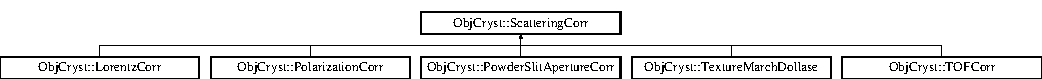
\includegraphics[height=1.056604cm]{a00088}
\end{center}
\end{figure}
\subsubsection*{\-Public \-Member \-Functions}
\begin{DoxyCompactItemize}
\item 
{\bf \-Scattering\-Corr} (const {\bf \-Scattering\-Data} \&data)\label{a00088_ac1e37a73b0a107f66d1b1d75b9db9c47}

\begin{DoxyCompactList}\small\item\em \-Constructor, with the associated \doxyref{\-Scattering\-Data}{p.}{a00089} object. \end{DoxyCompactList}\item 
virtual const string \& {\bf \-Get\-Name} () const =0\label{a00088_adb2782d4e32cbcb89e2e69b3c8ad66fb}

\begin{DoxyCompactList}\small\item\em \-Get the name of this object. \end{DoxyCompactList}\item 
virtual const string \& {\bf \-Get\-Class\-Name} () const =0\label{a00088_a6d72e7a6ffff0c16d86930d9e72c6673}

\begin{DoxyCompactList}\small\item\em \-Get the name of the class. \end{DoxyCompactList}\item 
const \-Cryst\-Vector\-\_\-\-R\-E\-A\-L \& {\bf \-Get\-Corr} () const 
\begin{DoxyCompactList}\small\item\em \-Get the vector of corrections for all reflections. \end{DoxyCompactList}\item 
const {\bf \-Refinable\-Obj\-Clock} \& {\bf \-Get\-Clock\-Corr} () const \label{a00088_a4c5bead3a47202db88495e3d123c5927}

\begin{DoxyCompactList}\small\item\em \-Get the value of the clock corresponding to the last time the correction was actually computed. \end{DoxyCompactList}\end{DoxyCompactItemize}
\subsubsection*{\-Protected \-Member \-Functions}
\begin{DoxyCompactItemize}
\item 
virtual void {\bf \-Calc\-Corr} () const =0\label{a00088_a437a916156f6d88c76cb01ca4c748c89}

\begin{DoxyCompactList}\small\item\em \-Do the computation of corrected intensities. \end{DoxyCompactList}\end{DoxyCompactItemize}
\subsubsection*{\-Protected \-Attributes}
\begin{DoxyCompactItemize}
\item 
const {\bf \-Scattering\-Data} $\ast$ {\bf mp\-Data}\label{a00088_a0fa066328104835ff72ddf98687c8513}

\begin{DoxyCompactList}\small\item\em \-The associated \doxyref{\-Scattering\-Data}{p.}{a00089} object. \end{DoxyCompactList}\item 
\-Cryst\-Vector\-\_\-\-R\-E\-A\-L {\bf m\-Corr}\label{a00088_a7669922ac4bbdfb826748148d4016088}

\begin{DoxyCompactList}\small\item\em \-The vector of correction to intensities. \end{DoxyCompactList}\item 
{\bf \-Refinable\-Obj\-Clock} {\bf m\-Clock\-Corr\-Calc}\label{a00088_aa969418138a9d1867797857318d6f303}

\begin{DoxyCompactList}\small\item\em \-The clock marking the last time the correction was calculated. \end{DoxyCompactList}\end{DoxyCompactItemize}


\subsubsection{\-Detailed \-Description}
\-Base class to compute all kind of corrections to intensities\-: \-Lorentz, \-Polar, absorption, texcture, extinction, etc... 

\-The computed intensities are to be multiplied by all the \doxyref{\-Scattering\-Corr}{p.}{a00088} calculated.

\-This is an abstract base class. 

\subsubsection{\-Member \-Function \-Documentation}
\index{\-Obj\-Cryst\-::\-Scattering\-Corr@{\-Obj\-Cryst\-::\-Scattering\-Corr}!\-Get\-Corr@{\-Get\-Corr}}
\index{\-Get\-Corr@{\-Get\-Corr}!ObjCryst::ScatteringCorr@{\-Obj\-Cryst\-::\-Scattering\-Corr}}
\paragraph[{\-Get\-Corr}]{\setlength{\rightskip}{0pt plus 5cm}const \-Cryst\-Vector\-\_\-\-R\-E\-A\-L\& {\bf \-Obj\-Cryst\-::\-Scattering\-Corr\-::\-Get\-Corr} (
\begin{DoxyParamCaption}
{}
\end{DoxyParamCaption}
) const}\label{a00088_a50395369eb93155bf278453ba158f8cb}


\-Get the vector of corrections for all reflections. 

\-Calculated values must be multiplied by these values. 

\-The documentation for this class was generated from the following file\-:\begin{DoxyCompactItemize}
\item 
\-Scattering\-Corr.\-h\end{DoxyCompactItemize}

\subsection{ObjCryst::ScatteringPower Class Reference}
\label{a00089}\index{ObjCryst::ScatteringPower@{ObjCryst::ScatteringPower}}


Abstract Base Class to describe the scattering power of any \doxyref{Scatterer}{p.}{a00084} component in a crystal.  
Inheritance diagram for ObjCryst::ScatteringPower::\begin{figure}[H]
\begin{center}
\leavevmode
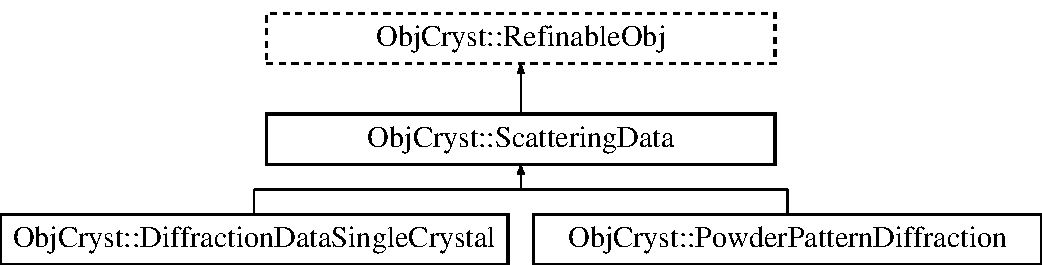
\includegraphics[height=2.66667cm]{a00089}
\end{center}
\end{figure}
\subsubsection*{Public Member Functions}
\begin{DoxyCompactItemize}
\item 
{\bfseries ScatteringPower} (const {\bf ScatteringPower} \&old)\label{a00089_a40d392b01f277a90affc2825ffa2e28d}

\item 
virtual const string \& {\bf GetClassName} () const 
\begin{DoxyCompactList}\small\item\em Name for this class (\char`\"{}RefinableObj\char`\"{}, \char`\"{}Crystal\char`\"{},. \item\end{DoxyCompactList}\item 
virtual void {\bfseries operator=} (const {\bf ScatteringPower} \&rhs)\label{a00089_a1db56ac3b61b4f5d1f70dbf65fff114a}

\item 
virtual CrystVector\_\-REAL {\bf GetScatteringFactor} (const {\bf ScatteringData} \&data, const int spgSymPosIndex=-\/1) const =0
\begin{DoxyCompactList}\small\item\em Get the Scattering factor for all reflections of a given \doxyref{ScatteringData}{p.}{a00088} object. \item\end{DoxyCompactList}\item 
virtual REAL {\bf GetForwardScatteringFactor} (const {\bf RadiationType}) const =0
\begin{DoxyCompactList}\small\item\em Get the scattering factor at (0,0,0). \item\end{DoxyCompactList}\item 
virtual CrystVector\_\-REAL {\bf GetTemperatureFactor} (const {\bf ScatteringData} \&data, const int spgSymPosIndex=-\/1) const =0
\begin{DoxyCompactList}\small\item\em Get the temperature factor for all reflections of a given \doxyref{ScatteringData}{p.}{a00088} object. \item\end{DoxyCompactList}\item 
virtual CrystMatrix\_\-REAL {\bf GetResonantScattFactReal} (const {\bf ScatteringData} \&data, const int spgSymPosIndex=-\/1) const =0
\begin{DoxyCompactList}\small\item\em Get the real part of the resonant scattering factor. \item\end{DoxyCompactList}\item 
virtual CrystMatrix\_\-REAL {\bf GetResonantScattFactImag} (const {\bf ScatteringData} \&data, const int spgSymPosIndex=-\/1) const =0
\begin{DoxyCompactList}\small\item\em Get the imaginary part of the resonant scattering factor. \item\end{DoxyCompactList}\item 
virtual bool {\bf IsScatteringFactorAnisotropic} () const \label{a00089_a0d099ca049eebbf23a31fb32b4229d4a}

\begin{DoxyCompactList}\small\item\em Is the scattering factor anisotropic ? \item\end{DoxyCompactList}\item 
virtual bool {\bf IsTemperatureFactorAnisotropic} () const \label{a00089_a602947d2e968b88f208d3507bd8a093d}

\begin{DoxyCompactList}\small\item\em Is the thermic factor anisotropic ? \item\end{DoxyCompactList}\item 
virtual bool {\bf IsResonantScatteringAnisotropic} () const \label{a00089_ac8f88b96383b0b97812913427d0c65f1}

\begin{DoxyCompactList}\small\item\em Are the resonant scattering terms anisotropic ? \item\end{DoxyCompactList}\item 
virtual const string \& {\bf GetSymbol} () const 
\begin{DoxyCompactList}\small\item\em Symbol for this Scattering power (the atom name for atoms). \item\end{DoxyCompactList}\item 
REAL {\bf GetBiso} () const 
\begin{DoxyCompactList}\small\item\em Returns the isotropic temperature B factor. \item\end{DoxyCompactList}\item 
REAL \& {\bf GetBiso} ()
\begin{DoxyCompactList}\small\item\em Returns the isotropic temperature B factor. \item\end{DoxyCompactList}\item 
virtual void {\bf SetBiso} (const REAL newB)
\begin{DoxyCompactList}\small\item\em Sets the isotropic temperature B factor. \item\end{DoxyCompactList}\item 
REAL {\bf GetBij} (const size\_\-t \&i, const size\_\-t \&j) const \label{a00089_aab538c7888aa57c38236bd01c9252965}

\begin{DoxyCompactList}\small\item\em Returns the anisotropic temperature B factor for (i, j) pair. \item\end{DoxyCompactList}\item 
REAL {\bf GetBij} (const size\_\-t \&idx) const 
\begin{DoxyCompactList}\small\item\em Returns the anisotropic temperature B factor for given index. \item\end{DoxyCompactList}\item 
virtual void {\bf SetBij} (const size\_\-t \&i, const size\_\-t \&j, const REAL newB)\label{a00089_a8c947f00897876d91f68617772a20dad}

\begin{DoxyCompactList}\small\item\em Sets the anisotropic temperature B factor for (i, j) pair. \item\end{DoxyCompactList}\item 
virtual void {\bf SetBij} (const size\_\-t \&idx, const REAL newB)
\begin{DoxyCompactList}\small\item\em Sets the anisotropic temperature B factor for given index. \item\end{DoxyCompactList}\item 
bool {\bf IsIsotropic} () const \label{a00089_a05909fe082739c6be397299813418618}

\begin{DoxyCompactList}\small\item\em Returns true if the scattering power is isotropic, else false. \item\end{DoxyCompactList}\item 
long {\bf GetDynPopCorrIndex} () const 
\begin{DoxyCompactList}\small\item\em Get the number identifying this kind of scatterer, used to decide whether two scatterers are equivalent, for the dynamical occupancy correction. \item\end{DoxyCompactList}\item 
long {\bf GetNbScatteringPower} () const \label{a00089_af7cf02d1229e45220953b345a6f6d427}

\begin{DoxyCompactList}\small\item\em Total number of \doxyref{ScatteringPower}{p.}{a00089} object. \item\end{DoxyCompactList}\item 
const {\bf RefinableObjClock} \& {\bf GetLastChangeClock} () const \label{a00089_aac5f03782e5b08b3e60254b1fe0aad4a}

\begin{DoxyCompactList}\small\item\em ObjCrystClock time when the last modification was made to the object. \item\end{DoxyCompactList}\item 
const string \& {\bf GetColourName} () const \label{a00089_acbe6442c66fcb7760b2684ec4d9456cd}

\begin{DoxyCompactList}\small\item\em Get the (POV-\/Ray) name associated to the color (if any). \item\end{DoxyCompactList}\item 
const float $\ast$ {\bf GetColourRGB} () const \label{a00089_a5a992fe0ab82ddc79f184bbb12d6aaa0}

\begin{DoxyCompactList}\small\item\em Get the float[3] array of RGB components defining the colour of this scattering power. \item\end{DoxyCompactList}\item 
void {\bf SetColour} (const string \&colorName)\label{a00089_ac48cb91ee4361a14d829227023479514}

\begin{DoxyCompactList}\small\item\em Set the colour from the associated POV-\/Ray name. \item\end{DoxyCompactList}\item 
void {\bf SetColour} (const float r, const float g, const float b)\label{a00089_a312da0ad4d8229baf7d6ab7ff9c45a3c}

\begin{DoxyCompactList}\small\item\em Set the colour from RGB components (all between 0 and 1.). \item\end{DoxyCompactList}\item 
virtual REAL {\bf GetRadius} () const =0
\begin{DoxyCompactList}\small\item\em Return the physical radius of this type of scatterer (for 3D display purposes). \item\end{DoxyCompactList}\item 
virtual void {\bf GetGeneGroup} (const {\bf RefinableObj} \&obj, CrystVector\_\-uint \&groupIndex, unsigned int \&firstGroup) const 
\begin{DoxyCompactList}\small\item\em Get the gene group assigned to each parameter. \item\end{DoxyCompactList}\item 
REAL {\bf GetMaximumLikelihoodPositionError} () const 
\begin{DoxyCompactList}\small\item\em Maximum Likelihood: get the estimated error (sigma) on the positions for this kind of element. \item\end{DoxyCompactList}\item 
void {\bf SetMaximumLikelihoodPositionError} (const REAL mle)
\begin{DoxyCompactList}\small\item\em Maximum Likelihood: set the estimated error (sigma) on the positions for this kind of element. \item\end{DoxyCompactList}\item 
REAL {\bf GetMaximumLikelihoodNbGhostAtom} () const \label{a00089_a23031fcb8c8c79d0e086da6aaadcd40c}

\begin{DoxyCompactList}\small\item\em Maximum Likelihood: get the number of ghost elements per asymmetric unit. \item\end{DoxyCompactList}\item 
void {\bf SetMaximumLikelihoodNbGhostAtom} (const REAL nb)\label{a00089_aa3343885c4b3b9d41c386f7d8aaacd63}

\begin{DoxyCompactList}\small\item\em Maximum Likelihood: set the number of ghost elements per asymmetric unit. \item\end{DoxyCompactList}\item 
const {\bf RefinableObjClock} \& {\bf GetMaximumLikelihoodParClock} () const 
\begin{DoxyCompactList}\small\item\em Get the clock value for the last change on the maximum likelihood parameters (positionnal error, number of ghost atoms). \item\end{DoxyCompactList}\item 
virtual REAL {\bfseries GetFormalCharge} () const \label{a00089_a04f10b6898e5242548a6980b99a55bb9}

\item 
virtual void {\bfseries SetFormalCharge} (const REAL charge)\label{a00089_a98c9fe3af63a4093a354bb814730aa76}

\end{DoxyCompactItemize}
\subsubsection*{Protected Member Functions}
\begin{DoxyCompactItemize}
\item 
virtual void {\bfseries InitRefParList} ()=0\label{a00089_a963cfe56b67286007bb93c7962e72b5c}

\item 
virtual void {\bf Init} ()\label{a00089_ac39b1294c085edac4c7180b4373a73c0}

\begin{DoxyCompactList}\small\item\em Initialization of the object, used by all constructors, and operator=. \item\end{DoxyCompactList}\item 
virtual void {\bf InitRGBColour} ()\label{a00089_a24c0c49adab2efe6af63c4915d861577}

\begin{DoxyCompactList}\small\item\em Get RGB Colour coordinates from Colour Name. \item\end{DoxyCompactList}\end{DoxyCompactItemize}
\subsubsection*{Protected Attributes}
\begin{DoxyCompactItemize}
\item 
long {\bf mDynPopCorrIndex}
\begin{DoxyCompactList}\small\item\em number identifying this kind of scatterer, for the dynamical occupancy correction. \item\end{DoxyCompactList}\item 
REAL {\bf mBiso}\label{a00089_aad32a210a13475061a2cda7525e05501}

\begin{DoxyCompactList}\small\item\em Temperature isotropic B factor. \item\end{DoxyCompactList}\item 
bool {\bf mIsIsotropic}\label{a00089_a312928a0ead2f2bff84156e772752fe1}

\begin{DoxyCompactList}\small\item\em Is the scattering isotropic ? \item\end{DoxyCompactList}\item 
CrystVector\_\-REAL {\bf mBeta}\label{a00089_a02a4524640e2d23805df26b114be680f}

\begin{DoxyCompactList}\small\item\em Anisotropic Beta(ij). \item\end{DoxyCompactList}\item 
{\bf RefinableObjClock} {\bf mClock}\label{a00089_a7b2e1854b0799312da38819cebf13672}

\begin{DoxyCompactList}\small\item\em Clock. \item\end{DoxyCompactList}\item 
string {\bf mColourName}\label{a00089_a0726f45b1f31f338326a28345b57738e}

\begin{DoxyCompactList}\small\item\em Colour for this \doxyref{ScatteringPower}{p.}{a00089} (from POVRay). \item\end{DoxyCompactList}\item 
float {\bf mColourRGB} [3]\label{a00089_a00cf7e1fbe362a96be4a22c8b454fd29}

\begin{DoxyCompactList}\small\item\em Colour for this \doxyref{ScatteringPower}{p.}{a00089} using RGB. \item\end{DoxyCompactList}\item 
REAL {\bf mMaximumLikelihoodPositionError}\label{a00089_a20aa001aad26734367838792eff09682}

\begin{DoxyCompactList}\small\item\em estimated error (sigma) on the positions for this type of element. \item\end{DoxyCompactList}\item 
{\bf RefinableObjClock} {\bfseries mMaximumLikelihoodParClock}\label{a00089_a727c82cdb03968dba28c5f7549860093}

\item 
REAL {\bf mMaximumLikelihoodNbGhost}
\begin{DoxyCompactList}\small\item\em Number of ghost atoms in the asymmetric unit. \item\end{DoxyCompactList}\item 
REAL {\bf mFormalCharge}
\begin{DoxyCompactList}\small\item\em Formal Charge. \item\end{DoxyCompactList}\end{DoxyCompactItemize}


\subsubsection{Detailed Description}
Abstract Base Class to describe the scattering power of any \doxyref{Scatterer}{p.}{a00084} component in a crystal. This includes:
\begin{DoxyItemize}
\item the scattering factor,
\item the temperature factor
\item real and imaginary parts of the resonant scattering factor.
\end{DoxyItemize}

The interface is independent of the radiation type.

This base class is designed to handle both isotropic and anisotropic versions of scattering, temperature and anomalous factors.

\begin{Desc}
\item[{\bf Todo}]Anisotropic scattering (temperature factor especially) code, using derived classes 

Clarify organization by removing any 'real' data from the top, abstract base class (eg remove Biso and Betaij), and by creating derived classes. Optionnaly 3 classes (used as members of \doxyref{ScatteringPower}{p.}{a00089}) could be created, TemperatureFactor, ScatteringFactor, and ResonantScatteringFactor. In any way the design of this class should not evolve, so that code using the \doxyref{ScatteringPower}{p.}{a00089} interface will remain compatible whatever modifications are made. \end{Desc}


\subsubsection{Member Function Documentation}
\index{ObjCryst::ScatteringPower@{ObjCryst::ScatteringPower}!GetBij@{GetBij}}
\index{GetBij@{GetBij}!ObjCryst::ScatteringPower@{ObjCryst::ScatteringPower}}
\paragraph[{GetBij}]{\setlength{\rightskip}{0pt plus 5cm}REAL ObjCryst::ScatteringPower::GetBij (const size\_\-t \& {\em idx}) const}\hfill\label{a00089_abc78b680e9cd6a38b875731363978477}


Returns the anisotropic temperature B factor for given index. 0 -\/$>$ (1, 1) 1 -\/$>$ (2, 2) 2 -\/$>$ (3, 3) 3 -\/$>$ (1, 2) 4 -\/$>$ (1, 3) 5 -\/$>$ (2, 3) \index{ObjCryst::ScatteringPower@{ObjCryst::ScatteringPower}!GetBiso@{GetBiso}}
\index{GetBiso@{GetBiso}!ObjCryst::ScatteringPower@{ObjCryst::ScatteringPower}}
\paragraph[{GetBiso}]{\setlength{\rightskip}{0pt plus 5cm}REAL\& ObjCryst::ScatteringPower::GetBiso ()}\hfill\label{a00089_ace567e5b32673e14521ae262388dfed6}


Returns the isotropic temperature B factor. \index{ObjCryst::ScatteringPower@{ObjCryst::ScatteringPower}!GetBiso@{GetBiso}}
\index{GetBiso@{GetBiso}!ObjCryst::ScatteringPower@{ObjCryst::ScatteringPower}}
\paragraph[{GetBiso}]{\setlength{\rightskip}{0pt plus 5cm}REAL ObjCryst::ScatteringPower::GetBiso () const}\hfill\label{a00089_ac3e116b2d956c229b11c98c837e042d8}


Returns the isotropic temperature B factor. \index{ObjCryst::ScatteringPower@{ObjCryst::ScatteringPower}!GetClassName@{GetClassName}}
\index{GetClassName@{GetClassName}!ObjCryst::ScatteringPower@{ObjCryst::ScatteringPower}}
\paragraph[{GetClassName}]{\setlength{\rightskip}{0pt plus 5cm}virtual const string\& ObjCryst::ScatteringPower::GetClassName () const\hspace{0.3cm}{\ttfamily  [virtual]}}\hfill\label{a00089_ac31cc4135011046f93d49f4173aee3ee}


Name for this class (\char`\"{}RefinableObj\char`\"{}, \char`\"{}Crystal\char`\"{},. ..). This is only useful to distinguish different classes when picking up objects from the \doxyref{RefinableObj}{p.}{a00070} Global Registry 

Reimplemented from {\bf ObjCryst::RefinableObj} \doxyref{}{p.}{a00070_a62968d90a7a3080738b363934616c019}.

Reimplemented in {\bf ObjCryst::ScatteringPowerAtom} \doxyref{}{p.}{a00090_a87fcc8fe4871d1b9b6ec08af5f353657}, and {\bf ObjCryst::ScatteringPowerSphere} \doxyref{}{p.}{a00091_a57e85d29926fe93da66041a43583e893}.\index{ObjCryst::ScatteringPower@{ObjCryst::ScatteringPower}!GetDynPopCorrIndex@{GetDynPopCorrIndex}}
\index{GetDynPopCorrIndex@{GetDynPopCorrIndex}!ObjCryst::ScatteringPower@{ObjCryst::ScatteringPower}}
\paragraph[{GetDynPopCorrIndex}]{\setlength{\rightskip}{0pt plus 5cm}long ObjCryst::ScatteringPower::GetDynPopCorrIndex () const}\hfill\label{a00089_ae3d48856abf5c8ef9dea6204309897bc}


Get the number identifying this kind of scatterer, used to decide whether two scatterers are equivalent, for the dynamical occupancy correction. \index{ObjCryst::ScatteringPower@{ObjCryst::ScatteringPower}!GetForwardScatteringFactor@{GetForwardScatteringFactor}}
\index{GetForwardScatteringFactor@{GetForwardScatteringFactor}!ObjCryst::ScatteringPower@{ObjCryst::ScatteringPower}}
\paragraph[{GetForwardScatteringFactor}]{\setlength{\rightskip}{0pt plus 5cm}virtual REAL ObjCryst::ScatteringPower::GetForwardScatteringFactor (const  {\em RadiationType}) const\hspace{0.3cm}{\ttfamily  [pure virtual]}}\hfill\label{a00089_a854b51b9b08e96af0fe7986fe372c50c}


Get the scattering factor at (0,0,0). Used for scatterer (electron, nucleus) density generation. 

Implemented in {\bf ObjCryst::ScatteringPowerAtom} \doxyref{}{p.}{a00090_ab979c1f31fd03b0f10f0afd625be722e}, {\bf ObjCryst::ScatteringPowerSphere} \doxyref{}{p.}{a00091_a9bd142cc8112495d41393b4faffc4fcd}, and {\bf ObjCryst::GlobalScatteringPower} \doxyref{}{p.}{a00034_a33c01c7512929a947e6489df41edf7b3}.\index{ObjCryst::ScatteringPower@{ObjCryst::ScatteringPower}!GetGeneGroup@{GetGeneGroup}}
\index{GetGeneGroup@{GetGeneGroup}!ObjCryst::ScatteringPower@{ObjCryst::ScatteringPower}}
\paragraph[{GetGeneGroup}]{\setlength{\rightskip}{0pt plus 5cm}virtual void ObjCryst::ScatteringPower::GetGeneGroup (const {\bf RefinableObj} \& {\em obj}, \/  CrystVector\_\-uint \& {\em groupIndex}, \/  unsigned int \& {\em firstGroup}) const\hspace{0.3cm}{\ttfamily  [virtual]}}\hfill\label{a00089_aae98160e01ecb2098cf4777126860aa5}


Get the gene group assigned to each parameter. Each parameter (a {\itshape gene\/} in terms of genetic algorithms) can be assigned to a gene group. Thus when mating two configurations, genes will be exchanged by groups. By default (in the base RefinabeObj class), each parameter is alone in its group. Derived classes can group genes for a better s$\ast$$\ast$ life.

The number identifying a gene group only has a meaning in a given object. It can also change on subsequent calls, and thus is not unique.


\begin{DoxyParams}{Parameters}
\item[{\em obj}]the , supplied by an algorithm class (\doxyref{OptimizationObj}{p.}{a00054},..), which contains a list of parameters, some of which (but possibly all or none) are parameters belonging to this object. \item[{\em groupIndex}]a vector of unsigned integers, one for each parameter in the input object, giving an unsigned integer value as gene group index. At the beginning this vector should contain only zeros (no group assigned). \item[{\em firstGroup}]this is the number of groups which have already been assigned, plus one. The gene groups returned by this object will start from this value, and increment {\bfseries firstGroup} for each gene group used, so that different \doxyref{RefinableObj}{p.}{a00070} cannot share a gene group. \end{DoxyParams}
\begin{DoxyNote}{Note}
this function is not optimized, and should only be called at the beginning of a refinement. 
\end{DoxyNote}


Reimplemented from {\bf ObjCryst::RefinableObj} \doxyref{}{p.}{a00070_ad59c8ad2b0d7ee59fa3f399a54f05e54}.\index{ObjCryst::ScatteringPower@{ObjCryst::ScatteringPower}!GetMaximumLikelihoodParClock@{GetMaximumLikelihoodParClock}}
\index{GetMaximumLikelihoodParClock@{GetMaximumLikelihoodParClock}!ObjCryst::ScatteringPower@{ObjCryst::ScatteringPower}}
\paragraph[{GetMaximumLikelihoodParClock}]{\setlength{\rightskip}{0pt plus 5cm}const {\bf RefinableObjClock}\& ObjCryst::ScatteringPower::GetMaximumLikelihoodParClock () const}\hfill\label{a00089_a63af7f309f1d9e03245f84ba21b1dc4e}


Get the clock value for the last change on the maximum likelihood parameters (positionnal error, number of ghost atoms). \index{ObjCryst::ScatteringPower@{ObjCryst::ScatteringPower}!GetMaximumLikelihoodPositionError@{GetMaximumLikelihoodPositionError}}
\index{GetMaximumLikelihoodPositionError@{GetMaximumLikelihoodPositionError}!ObjCryst::ScatteringPower@{ObjCryst::ScatteringPower}}
\paragraph[{GetMaximumLikelihoodPositionError}]{\setlength{\rightskip}{0pt plus 5cm}REAL ObjCryst::ScatteringPower::GetMaximumLikelihoodPositionError () const}\hfill\label{a00089_a34a36179228e07e92a85da9d17376649}


Maximum Likelihood: get the estimated error (sigma) on the positions for this kind of element. \index{ObjCryst::ScatteringPower@{ObjCryst::ScatteringPower}!GetRadius@{GetRadius}}
\index{GetRadius@{GetRadius}!ObjCryst::ScatteringPower@{ObjCryst::ScatteringPower}}
\paragraph[{GetRadius}]{\setlength{\rightskip}{0pt plus 5cm}virtual REAL ObjCryst::ScatteringPower::GetRadius () const\hspace{0.3cm}{\ttfamily  [pure virtual]}}\hfill\label{a00089_ac44860aca21734844379ddec87622f7b}


Return the physical radius of this type of scatterer (for 3D display purposes). \begin{DoxyWarning}{Warning}
this may be removed later. 
\end{DoxyWarning}


Implemented in {\bf ObjCryst::ScatteringPowerAtom} \doxyref{}{p.}{a00090_a38cdad845523d408f473cdea050841a0}, {\bf ObjCryst::ScatteringPowerSphere} \doxyref{}{p.}{a00091_a1f4b091f0990b959acb0645fd575a080}, and {\bf ObjCryst::GlobalScatteringPower} \doxyref{}{p.}{a00034_aadef1e0a463f70f4f70dba3d12dba9ed}.\index{ObjCryst::ScatteringPower@{ObjCryst::ScatteringPower}!GetResonantScattFactImag@{GetResonantScattFactImag}}
\index{GetResonantScattFactImag@{GetResonantScattFactImag}!ObjCryst::ScatteringPower@{ObjCryst::ScatteringPower}}
\paragraph[{GetResonantScattFactImag}]{\setlength{\rightskip}{0pt plus 5cm}virtual CrystMatrix\_\-REAL ObjCryst::ScatteringPower::GetResonantScattFactImag (const {\bf ScatteringData} \& {\em data}, \/  const int {\em spgSymPosIndex} = {\ttfamily -\/1}) const\hspace{0.3cm}{\ttfamily  [pure virtual]}}\hfill\label{a00089_a9bc5d86bf76116f645b43d46f2a9771c}


Get the imaginary part of the resonant scattering factor. \begin{DoxyReturn}{Returns}
a matrix where each row corresponds to each wavelength (currently only monochromatic experiments are made so there is only one row), and each column corresponds to each reflection {\itshape only\/} if the scattering term is anisotropic, which is not the case so far... 
\end{DoxyReturn}

\begin{DoxyParams}{Parameters}
\item[{\em data,:}]the \doxyref{ScatteringData}{p.}{a00088} object, giving access to all the reflections, and a list of wavelengths. \item[{\em spgSymPosIndex,:}]if the \doxyref{ScatteringPower}{p.}{a00089} is anisotropic, then the different symmetrics will not have the same scattering power for all reflections. This parameter is the index of the symmetric position in the Spacegroup. If spgSymPosIndex=-\/1, the isotropic values are returned. \end{DoxyParams}
\begin{DoxyWarning}{Warning}
There is no anisotropic code yet, so spgSymPosIndex is simply ignored so far , but the design of this function is general for any anisotropic scattering. 
\end{DoxyWarning}


Implemented in {\bf ObjCryst::ScatteringPowerAtom} \doxyref{}{p.}{a00090_a18e0f4ec2008406f6b6f770abada9b88}, {\bf ObjCryst::ScatteringPowerSphere} \doxyref{}{p.}{a00091_aee221744487a1c29023399b71e855c06}, and {\bf ObjCryst::GlobalScatteringPower} \doxyref{}{p.}{a00034_af3b5eefc24e2c60843793cdfbc240a11}.\index{ObjCryst::ScatteringPower@{ObjCryst::ScatteringPower}!GetResonantScattFactReal@{GetResonantScattFactReal}}
\index{GetResonantScattFactReal@{GetResonantScattFactReal}!ObjCryst::ScatteringPower@{ObjCryst::ScatteringPower}}
\paragraph[{GetResonantScattFactReal}]{\setlength{\rightskip}{0pt plus 5cm}virtual CrystMatrix\_\-REAL ObjCryst::ScatteringPower::GetResonantScattFactReal (const {\bf ScatteringData} \& {\em data}, \/  const int {\em spgSymPosIndex} = {\ttfamily -\/1}) const\hspace{0.3cm}{\ttfamily  [pure virtual]}}\hfill\label{a00089_a42c1302254787d13b9e0f2210315291a}


Get the real part of the resonant scattering factor. \begin{DoxyReturn}{Returns}
a matrix where each row corresponds to each wavelength (currently only monochromatic experiments are made so there is only one row), and each column corresponds to each reflection {\itshape only\/} if the scattering term is anisotropic, which is not the case so far... 
\end{DoxyReturn}

\begin{DoxyParams}{Parameters}
\item[{\em data,:}]the \doxyref{ScatteringData}{p.}{a00088} object, giving access to all the reflections and a list of wavelengths). \item[{\em spgSymPosIndex,:}]if the \doxyref{ScatteringPower}{p.}{a00089} is anisotropic, then the different symmetrics will not have the same scattering power for all reflections. This parameter is the index of the symmetric position in the Spacegroup. If spgSymPosIndex=-\/1, the isotropic values are returned. \end{DoxyParams}
\begin{DoxyWarning}{Warning}
There is no anisotropic code yet, so spgSymPosIndex is simply ignored so far , but the design of this function is general for any anisotropic scattering. 
\end{DoxyWarning}


Implemented in {\bf ObjCryst::ScatteringPowerAtom} \doxyref{}{p.}{a00090_a538841350c5a7147f7be607dd3ef5b72}, {\bf ObjCryst::ScatteringPowerSphere} \doxyref{}{p.}{a00091_a064671bfd711ef108be7a1528e52cd46}, and {\bf ObjCryst::GlobalScatteringPower} \doxyref{}{p.}{a00034_a9ddb16c057b744df58473fd2880baa3c}.\index{ObjCryst::ScatteringPower@{ObjCryst::ScatteringPower}!GetScatteringFactor@{GetScatteringFactor}}
\index{GetScatteringFactor@{GetScatteringFactor}!ObjCryst::ScatteringPower@{ObjCryst::ScatteringPower}}
\paragraph[{GetScatteringFactor}]{\setlength{\rightskip}{0pt plus 5cm}virtual CrystVector\_\-REAL ObjCryst::ScatteringPower::GetScatteringFactor (const {\bf ScatteringData} \& {\em data}, \/  const int {\em spgSymPosIndex} = {\ttfamily -\/1}) const\hspace{0.3cm}{\ttfamily  [pure virtual]}}\hfill\label{a00089_af18f3eaaf45af87bc3a2a0ff21bc34b6}


Get the Scattering factor for all reflections of a given \doxyref{ScatteringData}{p.}{a00088} object. \begin{DoxyReturn}{Returns}
a vector with the scattering factor for all reflections, in the same order as in the \doxyref{ScatteringData}{p.}{a00088} object. This format is independent of the radiation type (X-\/Ray, neutron..). 
\end{DoxyReturn}

\begin{DoxyParams}{Parameters}
\item[{\em data,:}]the \doxyref{ScatteringData}{p.}{a00088} object, giving access to all the reflections. \item[{\em spgSymPosIndex,:}]if the \doxyref{ScatteringPower}{p.}{a00089} is anisotropic, then the different symmetrics will not have the same scattering power for all reflections. This parameter is the index of the symmetric position in the Spacegroup. If spgSymPosIndex=-\/1, the isotropic values are returned. \end{DoxyParams}
\begin{DoxyWarning}{Warning}
There is no anisotropic code yet, so spgSymPosIndex is simply ignored so far , but the design of this function is general for any anisotropic scattering. 
\end{DoxyWarning}


Implemented in {\bf ObjCryst::ScatteringPowerAtom} \doxyref{}{p.}{a00090_a1c1733e6f6aab65fbe033b877cac5ae8}, {\bf ObjCryst::ScatteringPowerSphere} \doxyref{}{p.}{a00091_a073f08b17ba89e0ac5ed8e1a61cb04fe}, and {\bf ObjCryst::GlobalScatteringPower} \doxyref{}{p.}{a00034_acd525a54e45dc3c70fb5445b8b9b5a8c}.\index{ObjCryst::ScatteringPower@{ObjCryst::ScatteringPower}!GetSymbol@{GetSymbol}}
\index{GetSymbol@{GetSymbol}!ObjCryst::ScatteringPower@{ObjCryst::ScatteringPower}}
\paragraph[{GetSymbol}]{\setlength{\rightskip}{0pt plus 5cm}virtual const string\& ObjCryst::ScatteringPower::GetSymbol () const\hspace{0.3cm}{\ttfamily  [virtual]}}\hfill\label{a00089_a5cdd13d241974a6e6f0d3803256a3d10}


Symbol for this Scattering power (the atom name for atoms). 

Reimplemented in {\bf ObjCryst::ScatteringPowerAtom} \doxyref{}{p.}{a00090_a0b21c0253564cb40353171b182f50ecf}.\index{ObjCryst::ScatteringPower@{ObjCryst::ScatteringPower}!GetTemperatureFactor@{GetTemperatureFactor}}
\index{GetTemperatureFactor@{GetTemperatureFactor}!ObjCryst::ScatteringPower@{ObjCryst::ScatteringPower}}
\paragraph[{GetTemperatureFactor}]{\setlength{\rightskip}{0pt plus 5cm}virtual CrystVector\_\-REAL ObjCryst::ScatteringPower::GetTemperatureFactor (const {\bf ScatteringData} \& {\em data}, \/  const int {\em spgSymPosIndex} = {\ttfamily -\/1}) const\hspace{0.3cm}{\ttfamily  [pure virtual]}}\hfill\label{a00089_a3df723db77380c82ecff5f7050490255}


Get the temperature factor for all reflections of a given \doxyref{ScatteringData}{p.}{a00088} object. \begin{DoxyReturn}{Returns}
a vector with the temperature factor for all reflections, in the same order as in the \doxyref{ScatteringData}{p.}{a00088} object. 
\end{DoxyReturn}

\begin{DoxyParams}{Parameters}
\item[{\em data,:}]the \doxyref{ScatteringData}{p.}{a00088} object, giving access to all the reflections. \item[{\em spgSymPosIndex,:}]if the \doxyref{ScatteringPower}{p.}{a00089} is anisotropic, then the different symmetrics will not have the same scattering power for all reflections. This parameter is the index of the symmetric position in the Spacegroup. If spgSymPosIndex=-\/1, the isotropic values are returned. \end{DoxyParams}
\begin{DoxyWarning}{Warning}
There is no anisotropic code yet, so spgSymPosIndex is simply ignored so far , but the design of this function is general for any anisotropic scattering. 
\end{DoxyWarning}


Implemented in {\bf ObjCryst::ScatteringPowerAtom} \doxyref{}{p.}{a00090_aefe7a8b036c3f5a4a2b781b527dfa8c3}, {\bf ObjCryst::ScatteringPowerSphere} \doxyref{}{p.}{a00091_a3927291a20f5807c2ec6a9ae3627005d}, and {\bf ObjCryst::GlobalScatteringPower} \doxyref{}{p.}{a00034_a48da59604bb5a35fdac09087bc0fcff4}.\index{ObjCryst::ScatteringPower@{ObjCryst::ScatteringPower}!SetBij@{SetBij}}
\index{SetBij@{SetBij}!ObjCryst::ScatteringPower@{ObjCryst::ScatteringPower}}
\paragraph[{SetBij}]{\setlength{\rightskip}{0pt plus 5cm}virtual void ObjCryst::ScatteringPower::SetBij (const size\_\-t \& {\em idx}, \/  const REAL {\em newB})\hspace{0.3cm}{\ttfamily  [virtual]}}\hfill\label{a00089_a50b648d97ebb1ab97b39195b098eff50}


Sets the anisotropic temperature B factor for given index. 0 -\/$>$ (1, 1) 1 -\/$>$ (2, 2) 2 -\/$>$ (3, 3) 3 -\/$>$ (1, 2) 4 -\/$>$ (1, 3) 5 -\/$>$ (2, 3) \index{ObjCryst::ScatteringPower@{ObjCryst::ScatteringPower}!SetBiso@{SetBiso}}
\index{SetBiso@{SetBiso}!ObjCryst::ScatteringPower@{ObjCryst::ScatteringPower}}
\paragraph[{SetBiso}]{\setlength{\rightskip}{0pt plus 5cm}virtual void ObjCryst::ScatteringPower::SetBiso (const REAL {\em newB})\hspace{0.3cm}{\ttfamily  [virtual]}}\hfill\label{a00089_a179266106b89bcbb4885f9f20ce315c3}


Sets the isotropic temperature B factor. \index{ObjCryst::ScatteringPower@{ObjCryst::ScatteringPower}!SetMaximumLikelihoodPositionError@{SetMaximumLikelihoodPositionError}}
\index{SetMaximumLikelihoodPositionError@{SetMaximumLikelihoodPositionError}!ObjCryst::ScatteringPower@{ObjCryst::ScatteringPower}}
\paragraph[{SetMaximumLikelihoodPositionError}]{\setlength{\rightskip}{0pt plus 5cm}void ObjCryst::ScatteringPower::SetMaximumLikelihoodPositionError (const REAL {\em mle})}\hfill\label{a00089_aeba30efe61155572ffdada1121578bc9}


Maximum Likelihood: set the estimated error (sigma) on the positions for this kind of element. 

\subsubsection{Member Data Documentation}
\index{ObjCryst::ScatteringPower@{ObjCryst::ScatteringPower}!mDynPopCorrIndex@{mDynPopCorrIndex}}
\index{mDynPopCorrIndex@{mDynPopCorrIndex}!ObjCryst::ScatteringPower@{ObjCryst::ScatteringPower}}
\paragraph[{mDynPopCorrIndex}]{\setlength{\rightskip}{0pt plus 5cm}long {\bf ObjCryst::ScatteringPower::mDynPopCorrIndex}\hspace{0.3cm}{\ttfamily  [protected]}}\hfill\label{a00089_a0266da1d92ec3d14989a2d4047710c4b}


number identifying this kind of scatterer, for the dynamical occupancy correction. Right now it is the atomic number. \index{ObjCryst::ScatteringPower@{ObjCryst::ScatteringPower}!mFormalCharge@{mFormalCharge}}
\index{mFormalCharge@{mFormalCharge}!ObjCryst::ScatteringPower@{ObjCryst::ScatteringPower}}
\paragraph[{mFormalCharge}]{\setlength{\rightskip}{0pt plus 5cm}REAL {\bf ObjCryst::ScatteringPower::mFormalCharge}\hspace{0.3cm}{\ttfamily  [protected]}}\hfill\label{a00089_a030be52e5ba5540bf068e6be4ccb190e}


Formal Charge. This can be used for bond valence analysis, or energy calculations.

Default value is 0. \index{ObjCryst::ScatteringPower@{ObjCryst::ScatteringPower}!mMaximumLikelihoodNbGhost@{mMaximumLikelihoodNbGhost}}
\index{mMaximumLikelihoodNbGhost@{mMaximumLikelihoodNbGhost}!ObjCryst::ScatteringPower@{ObjCryst::ScatteringPower}}
\paragraph[{mMaximumLikelihoodNbGhost}]{\setlength{\rightskip}{0pt plus 5cm}REAL {\bf ObjCryst::ScatteringPower::mMaximumLikelihoodNbGhost}\hspace{0.3cm}{\ttfamily  [protected]}}\hfill\label{a00089_a53eeb0a26003df0bcf604817e2fbadf7}


Number of ghost atoms in the asymmetric unit. These contribute to the variance of the structure factor, but not to the structure factor as the uncertainty on their position is infinite. 

The documentation for this class was generated from the following file:\begin{DoxyCompactItemize}
\item 
ScatteringPower.h\end{DoxyCompactItemize}

\subsection{Obj\-Cryst\-:\-:Molecule\-:\-:Rotor\-Group Struct Reference}
\label{a00090}\index{Obj\-Cryst\-::\-Molecule\-::\-Rotor\-Group@{Obj\-Cryst\-::\-Molecule\-::\-Rotor\-Group}}


Defines a group of atoms which can be rotated around an axis defined by two other atoms.  


\subsubsection*{Public Member Functions}
\begin{DoxyCompactItemize}
\item 
{\bf Rotor\-Group} (const {\bf Mol\-Atom} \&at1, const {\bf Mol\-Atom} \&at2)
\begin{DoxyCompactList}\small\item\em Constructor, with the two atoms around which the rotation shall be made. \end{DoxyCompactList}\end{DoxyCompactItemize}
\subsubsection*{Public Attributes}
\begin{DoxyCompactItemize}
\item 
const {\bf Mol\-Atom} $\ast$ {\bf mp\-Atom1}\label{a00090_a58f9b6ed1fc288d547a1617b17e75316}

\begin{DoxyCompactList}\small\item\em The first atom defining the rotation axis. \end{DoxyCompactList}\item 
const {\bf Mol\-Atom} $\ast$ {\bf mp\-Atom2}\label{a00090_ae6829772d661cbdef458f20a6d2d83a6}

\begin{DoxyCompactList}\small\item\em The second atom defining the rotation axis. \end{DoxyCompactList}\item 
set$<$ {\bf Mol\-Atom} $\ast$ $>$ {\bf mv\-Rotated\-Atom\-List}\label{a00090_a2ff8b0fdb5c57289ffbc53f301331caa}

\begin{DoxyCompactList}\small\item\em The set of atoms that are to be rotated. \end{DoxyCompactList}\item 
R\-E\-A\-L {\bf m\-Base\-Rotation\-Amplitude}
\begin{DoxyCompactList}\small\item\em The recommended rotation amplitude, for a base global optimization displacement, to obtain an average 0.\-1 Angstroem displacement per atom (pi$\ast$0.04 by default) \end{DoxyCompactList}\end{DoxyCompactItemize}


\subsubsection{Detailed Description}
Defines a group of atoms which can be rotated around an axis defined by two other atoms. 

\subsubsection{Constructor \& Destructor Documentation}
\index{Obj\-Cryst\-::\-Molecule\-::\-Rotor\-Group@{Obj\-Cryst\-::\-Molecule\-::\-Rotor\-Group}!Rotor\-Group@{Rotor\-Group}}
\index{Rotor\-Group@{Rotor\-Group}!ObjCryst::Molecule::RotorGroup@{Obj\-Cryst\-::\-Molecule\-::\-Rotor\-Group}}
\paragraph[{Rotor\-Group}]{\setlength{\rightskip}{0pt plus 5cm}Obj\-Cryst\-::\-Molecule\-::\-Rotor\-Group\-::\-Rotor\-Group (
\begin{DoxyParamCaption}
\item[{const {\bf Mol\-Atom} \&}]{at1, }
\item[{const {\bf Mol\-Atom} \&}]{at2}
\end{DoxyParamCaption}
)}\label{a00090_a04efc612bcdfd3c84132e6dc0c54bf92}


Constructor, with the two atoms around which the rotation shall be made. 

The list of atoms to be rotated is initially empty. 

\subsubsection{Member Data Documentation}
\index{Obj\-Cryst\-::\-Molecule\-::\-Rotor\-Group@{Obj\-Cryst\-::\-Molecule\-::\-Rotor\-Group}!m\-Base\-Rotation\-Amplitude@{m\-Base\-Rotation\-Amplitude}}
\index{m\-Base\-Rotation\-Amplitude@{m\-Base\-Rotation\-Amplitude}!ObjCryst::Molecule::RotorGroup@{Obj\-Cryst\-::\-Molecule\-::\-Rotor\-Group}}
\paragraph[{m\-Base\-Rotation\-Amplitude}]{\setlength{\rightskip}{0pt plus 5cm}R\-E\-A\-L Obj\-Cryst\-::\-Molecule\-::\-Rotor\-Group\-::m\-Base\-Rotation\-Amplitude}\label{a00090_ab98013a7f74a26ebe8d04c066f9ea49d}


The recommended rotation amplitude, for a base global optimization displacement, to obtain an average 0.\-1 Angstroem displacement per atom (pi$\ast$0.04 by default) 

This is learnt at the beginning of an optimization, i.\-e. in \doxyref{Molecule\-::\-Build\-Rotor\-Group()}{p.}{a00054_a3642fa8104faa1ce84a977600f9d1aeb} 

The documentation for this struct was generated from the following file\-:\begin{DoxyCompactItemize}
\item 
Molecule.\-h\end{DoxyCompactItemize}

\subsection{\-Obj\-Cryst\-:\-:\-Scattering\-Power\-Atom \-Class \-Reference}
\label{a00091}\index{\-Obj\-Cryst\-::\-Scattering\-Power\-Atom@{\-Obj\-Cryst\-::\-Scattering\-Power\-Atom}}


\-The \-Scattering \-Power for an \doxyref{\-Atom}{p.}{a00008}.  


\-Inheritance diagram for \-Obj\-Cryst\-:\-:\-Scattering\-Power\-Atom\-:\begin{figure}[H]
\begin{center}
\leavevmode
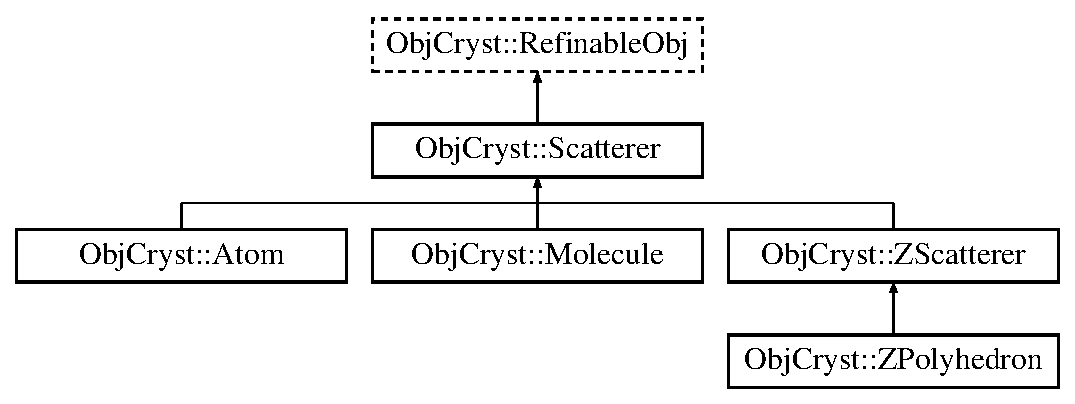
\includegraphics[height=3.000000cm]{a00091}
\end{center}
\end{figure}
\subsubsection*{\-Public \-Member \-Functions}
\begin{DoxyCompactItemize}
\item 
{\bf \-Scattering\-Power\-Atom} (const string \&name, const string \&symbol, const \-R\-E\-A\-L b\-Iso=1.\-0)
\begin{DoxyCompactList}\small\item\em \doxyref{\-Atom}{p.}{a00008} constructor. \end{DoxyCompactList}\item 
{\bfseries \-Scattering\-Power\-Atom} (const {\bf \-Scattering\-Power\-Atom} \&old)\label{a00091_a72487203dd97ef8a5701f451bb23b644}

\item 
virtual const string \& {\bf \-Get\-Class\-Name} () const 
\begin{DoxyCompactList}\small\item\em \-Name for this class (\char`\"{}\-Refinable\-Obj\char`\"{}, \char`\"{}\-Crystal\char`\"{},...). \end{DoxyCompactList}\item 
void {\bf \-Init} (const string \&name, const string \&symbol, const \-R\-E\-A\-L b\-Iso=1.\-0)\label{a00091_a7f599ee186028c6d065d39b13b15a194}

\begin{DoxyCompactList}\small\item\em \-Re-\/initialize parameters (after using the default constructor). \end{DoxyCompactList}\item 
virtual \-Cryst\-Vector\-\_\-\-R\-E\-A\-L {\bf \-Get\-Scattering\-Factor} (const {\bf \-Scattering\-Data} \&data, const int spg\-Sym\-Pos\-Index=0) const 
\begin{DoxyCompactList}\small\item\em \-Get the \-Scattering factor for all reflections of a given \doxyref{\-Scattering\-Data}{p.}{a00089} object. \end{DoxyCompactList}\item 
virtual \-R\-E\-A\-L {\bf \-Get\-Forward\-Scattering\-Factor} (const {\bf \-Radiation\-Type}) const 
\begin{DoxyCompactList}\small\item\em \-Get the scattering factor at (0,0,0). \end{DoxyCompactList}\item 
virtual \-Cryst\-Vector\-\_\-\-R\-E\-A\-L {\bf \-Get\-Temperature\-Factor} (const {\bf \-Scattering\-Data} \&data, const int spg\-Sym\-Pos\-Index=0) const 
\begin{DoxyCompactList}\small\item\em \-Get the temperature factor for all reflections of a given \doxyref{\-Scattering\-Data}{p.}{a00089} object. \end{DoxyCompactList}\item 
virtual \-Cryst\-Matrix\-\_\-\-R\-E\-A\-L {\bf \-Get\-Resonant\-Scatt\-Fact\-Real} (const {\bf \-Scattering\-Data} \&data, const int spg\-Sym\-Pos\-Index=0) const 
\begin{DoxyCompactList}\small\item\em \-Get the real part of the resonant scattering factor. \end{DoxyCompactList}\item 
virtual \-Cryst\-Matrix\-\_\-\-R\-E\-A\-L {\bf \-Get\-Resonant\-Scatt\-Fact\-Imag} (const {\bf \-Scattering\-Data} \&data, const int spg\-Sym\-Pos\-Index=0) const 
\begin{DoxyCompactList}\small\item\em \-Get the imaginary part of the resonant scattering factor. \end{DoxyCompactList}\item 
void {\bf \-Set\-Symbol} (const string \&symbol)\label{a00091_a549de97e18838d040c1aa473122f762e}

\begin{DoxyCompactList}\small\item\em \-Set the symbol for this atom. \end{DoxyCompactList}\item 
virtual const string \& {\bf \-Get\-Symbol} () const \label{a00091_a0b21c0253564cb40353171b182f50ecf}

\begin{DoxyCompactList}\small\item\em \-Returns the symbol ('\-Ta', '\-O2-\/',...) of the atom. \end{DoxyCompactList}\item 
string {\bf \-Get\-Element\-Name} () const 
\begin{DoxyCompactList}\small\item\em \-Returns the standard name of the element (ie \char`\"{}hydrogen\char`\"{}, \char`\"{}tantalum\char`\"{},..). \end{DoxyCompactList}\item 
int {\bf \-Get\-Atomic\-Number} () const \label{a00091_ab9b1734d7c2edd81ef1c16d3c7e84745}

\begin{DoxyCompactList}\small\item\em \-Atomic number for this atom. \end{DoxyCompactList}\item 
\-R\-E\-A\-L {\bf \-Get\-Radius} () const \label{a00091_a38cdad845523d408f473cdea050841a0}

\begin{DoxyCompactList}\small\item\em \-Atomic radius for this atom, in \-Angstroems. \end{DoxyCompactList}\item 
virtual void {\bfseries \-Print} () const \label{a00091_a8e62f81f3e2f5016942d5cb3de688d02}

\item 
virtual void {\bf \-X\-M\-L\-Output} (ostream \&os, int indent=0) const 
\begin{DoxyCompactList}\small\item\em \-Output to stream in well-\/formed \-X\-M\-L. \end{DoxyCompactList}\item 
virtual void {\bf \-X\-M\-L\-Input} (istream \&is, const {\bf \-X\-M\-L\-Cryst\-Tag} \&tag)
\begin{DoxyCompactList}\small\item\em \-Input \-From stream. \end{DoxyCompactList}\end{DoxyCompactItemize}
\subsubsection*{\-Protected \-Member \-Functions}
\begin{DoxyCompactItemize}
\item 
void {\bf \-Init\-At\-Scatt\-Coeffs\-W\-K95} ()
\item 
void {\bf \-Init\-At\-Neutron\-Scatt\-Coeffs} ()
\item 
virtual void {\bfseries \-Init\-Ref\-Par\-List} ()\label{a00091_aa3a14df260e9fba70ebe82249a20d560}

\end{DoxyCompactItemize}
\subsubsection*{\-Protected \-Attributes}
\begin{DoxyCompactItemize}
\item 
string {\bf m\-Symbol}
\begin{DoxyCompactList}\small\item\em \-Symbol of this atom. \end{DoxyCompactList}\item 
int {\bf m\-Atomic\-Number}\label{a00091_ac849eb1448632e3866014aa66dc90805}

\begin{DoxyCompactList}\small\item\em atomic number (\-Z) for the atom \end{DoxyCompactList}\item 
cctbx\-::eltbx\-::xray\-\_\-scattering\-::gaussian $\ast$ {\bf mp\-Gaussian}\label{a00091_af5837e83fd8027adcaecde3a5fbb22f2}

\begin{DoxyCompactList}\small\item\em \-Pointer to cctbx's gaussian describing the thomson x-\/ray scattering factor. \end{DoxyCompactList}\item 
\-R\-E\-A\-L {\bf m\-Neutron\-Scatt\-Length\-Real}
\begin{DoxyCompactList}\small\item\em \-Neutron \-Bond \-Coherent \-Scattering lengths. \end{DoxyCompactList}\item 
\-R\-E\-A\-L {\bfseries m\-Neutron\-Scatt\-Length\-Imag}\label{a00091_a2ef56409065b0b7f84f4adae609097fc}

\item 
\-R\-E\-A\-L {\bf m\-Radius}\label{a00091_a45ddfa693e760f7250764e43425d3928}

\begin{DoxyCompactList}\small\item\em \-Radius of the atom, in \-Angstroems. \end{DoxyCompactList}\item 
\-R\-E\-A\-L {\bf m\-Neutron\-Abs\-Cross\-Section}
\begin{DoxyCompactList}\small\item\em \-Neutron \-Absorption cross section (barn) \end{DoxyCompactList}\end{DoxyCompactItemize}


\subsubsection{\-Detailed \-Description}
\-The \-Scattering \-Power for an \doxyref{\-Atom}{p.}{a00008}. 



\subsubsection{\-Constructor \& \-Destructor \-Documentation}
\index{\-Obj\-Cryst\-::\-Scattering\-Power\-Atom@{\-Obj\-Cryst\-::\-Scattering\-Power\-Atom}!\-Scattering\-Power\-Atom@{\-Scattering\-Power\-Atom}}
\index{\-Scattering\-Power\-Atom@{\-Scattering\-Power\-Atom}!ObjCryst::ScatteringPowerAtom@{\-Obj\-Cryst\-::\-Scattering\-Power\-Atom}}
\paragraph[{\-Scattering\-Power\-Atom}]{\setlength{\rightskip}{0pt plus 5cm}\-Obj\-Cryst\-::\-Scattering\-Power\-Atom\-::\-Scattering\-Power\-Atom (
\begin{DoxyParamCaption}
\item[{const string \&}]{name, }
\item[{const string \&}]{symbol, }
\item[{const \-R\-E\-A\-L}]{b\-Iso = {\ttfamily 1.0}}
\end{DoxyParamCaption}
)}\label{a00091_a9e77e9d0317491d62b392b891f0329e5}


\doxyref{\-Atom}{p.}{a00008} constructor. 


\begin{DoxyParams}{\-Parameters}
{\em symbol} & \-: '\-Ti' , '\-Ti4+', '\-Cl1-\/' \-These symbols {\itshape must\/} correspond to one of the entries of the international tables for crystallography (1995) giving the analytical approximation for scattering factors. \\
\hline
{\em name} & \-: name of the atom ('\-Ta1','\-Sm2', '\-Tungsten\-\_\-1'...). \-The name can have {\itshape any\/} format but spaces should be avoided, since it will generate problems when reading the names from a file... \\
\hline
{\em biso} & \-: \-Isotropic thermic coefficient \\
\hline
\end{DoxyParams}


\subsubsection{\-Member \-Function \-Documentation}
\index{\-Obj\-Cryst\-::\-Scattering\-Power\-Atom@{\-Obj\-Cryst\-::\-Scattering\-Power\-Atom}!\-Get\-Class\-Name@{\-Get\-Class\-Name}}
\index{\-Get\-Class\-Name@{\-Get\-Class\-Name}!ObjCryst::ScatteringPowerAtom@{\-Obj\-Cryst\-::\-Scattering\-Power\-Atom}}
\paragraph[{\-Get\-Class\-Name}]{\setlength{\rightskip}{0pt plus 5cm}virtual const string\& {\bf \-Obj\-Cryst\-::\-Scattering\-Power\-Atom\-::\-Get\-Class\-Name} (
\begin{DoxyParamCaption}
{}
\end{DoxyParamCaption}
) const\hspace{0.3cm}{\ttfamily  [virtual]}}\label{a00091_a87fcc8fe4871d1b9b6ec08af5f353657}


\-Name for this class (\char`\"{}\-Refinable\-Obj\char`\"{}, \char`\"{}\-Crystal\char`\"{},...). 

\-This is only useful to distinguish different classes when picking up objects from the \doxyref{\-Refinable\-Obj}{p.}{a00071} \-Global \-Registry 

\-Reimplemented from {\bf \-Obj\-Cryst\-::\-Scattering\-Power} \doxyref{}{p.}{a00090_ac31cc4135011046f93d49f4173aee3ee}.

\index{\-Obj\-Cryst\-::\-Scattering\-Power\-Atom@{\-Obj\-Cryst\-::\-Scattering\-Power\-Atom}!\-Get\-Element\-Name@{\-Get\-Element\-Name}}
\index{\-Get\-Element\-Name@{\-Get\-Element\-Name}!ObjCryst::ScatteringPowerAtom@{\-Obj\-Cryst\-::\-Scattering\-Power\-Atom}}
\paragraph[{\-Get\-Element\-Name}]{\setlength{\rightskip}{0pt plus 5cm}string {\bf \-Obj\-Cryst\-::\-Scattering\-Power\-Atom\-::\-Get\-Element\-Name} (
\begin{DoxyParamCaption}
{}
\end{DoxyParamCaption}
) const}\label{a00091_a37594e62e5ad0691b36a02ec9819ec74}


\-Returns the standard name of the element (ie \char`\"{}hydrogen\char`\"{}, \char`\"{}tantalum\char`\"{},..). 

\-Names are extracted form \-Grosse-\/\-Kunstleve 'atominfo' package, which uses data from the \-C\-R\-C \-Handbook of \-Chemistry \& \-Physics, 63rd \& 70th editions \index{\-Obj\-Cryst\-::\-Scattering\-Power\-Atom@{\-Obj\-Cryst\-::\-Scattering\-Power\-Atom}!\-Get\-Forward\-Scattering\-Factor@{\-Get\-Forward\-Scattering\-Factor}}
\index{\-Get\-Forward\-Scattering\-Factor@{\-Get\-Forward\-Scattering\-Factor}!ObjCryst::ScatteringPowerAtom@{\-Obj\-Cryst\-::\-Scattering\-Power\-Atom}}
\paragraph[{\-Get\-Forward\-Scattering\-Factor}]{\setlength{\rightskip}{0pt plus 5cm}virtual \-R\-E\-A\-L {\bf \-Obj\-Cryst\-::\-Scattering\-Power\-Atom\-::\-Get\-Forward\-Scattering\-Factor} (
\begin{DoxyParamCaption}
\item[{const {\bf \-Radiation\-Type}}]{}
\end{DoxyParamCaption}
) const\hspace{0.3cm}{\ttfamily  [virtual]}}\label{a00091_ab979c1f31fd03b0f10f0afd625be722e}


\-Get the scattering factor at (0,0,0). 

\-Used for scatterer (electron, nucleus) density generation. 

\-Implements {\bf \-Obj\-Cryst\-::\-Scattering\-Power} \doxyref{}{p.}{a00090_a854b51b9b08e96af0fe7986fe372c50c}.

\index{\-Obj\-Cryst\-::\-Scattering\-Power\-Atom@{\-Obj\-Cryst\-::\-Scattering\-Power\-Atom}!\-Get\-Resonant\-Scatt\-Fact\-Imag@{\-Get\-Resonant\-Scatt\-Fact\-Imag}}
\index{\-Get\-Resonant\-Scatt\-Fact\-Imag@{\-Get\-Resonant\-Scatt\-Fact\-Imag}!ObjCryst::ScatteringPowerAtom@{\-Obj\-Cryst\-::\-Scattering\-Power\-Atom}}
\paragraph[{\-Get\-Resonant\-Scatt\-Fact\-Imag}]{\setlength{\rightskip}{0pt plus 5cm}virtual \-Cryst\-Matrix\-\_\-\-R\-E\-A\-L {\bf \-Obj\-Cryst\-::\-Scattering\-Power\-Atom\-::\-Get\-Resonant\-Scatt\-Fact\-Imag} (
\begin{DoxyParamCaption}
\item[{const {\bf \-Scattering\-Data} \&}]{data, }
\item[{const int}]{spg\-Sym\-Pos\-Index = {\ttfamily 0}}
\end{DoxyParamCaption}
) const\hspace{0.3cm}{\ttfamily  [virtual]}}\label{a00091_a18e0f4ec2008406f6b6f770abada9b88}


\-Get the imaginary part of the resonant scattering factor. 

\begin{DoxyReturn}{\-Returns}
a matrix where each row corresponds to each wavelength (currently only monochromatic experiments are made so there is only one row), and each column corresponds to each reflection {\itshape only\/} if the scattering term is anisotropic, which is not the case so far... 
\end{DoxyReturn}

\begin{DoxyParams}{\-Parameters}
{\em data,\-:} & the \doxyref{\-Scattering\-Data}{p.}{a00089} object, giving access to all the reflections, and a list of wavelengths. \\
\hline
{\em spg\-Sym\-Pos\-Index,\-:} & if the \doxyref{\-Scattering\-Power}{p.}{a00090} is anisotropic, then the different symmetrics will not have the same scattering power for all reflections. \-This parameter is the index of the symmetric position in the \-Spacegroup. \-If spg\-Sym\-Pos\-Index=-\/1, the isotropic values are returned. \\
\hline
\end{DoxyParams}
\begin{DoxyWarning}{\-Warning}
\-There is no anisotropic code yet, so spg\-Sym\-Pos\-Index is simply ignored so far , but the design of this function is general for any anisotropic scattering. 
\end{DoxyWarning}


\-Implements {\bf \-Obj\-Cryst\-::\-Scattering\-Power} \doxyref{}{p.}{a00090_a9bc5d86bf76116f645b43d46f2a9771c}.

\index{\-Obj\-Cryst\-::\-Scattering\-Power\-Atom@{\-Obj\-Cryst\-::\-Scattering\-Power\-Atom}!\-Get\-Resonant\-Scatt\-Fact\-Real@{\-Get\-Resonant\-Scatt\-Fact\-Real}}
\index{\-Get\-Resonant\-Scatt\-Fact\-Real@{\-Get\-Resonant\-Scatt\-Fact\-Real}!ObjCryst::ScatteringPowerAtom@{\-Obj\-Cryst\-::\-Scattering\-Power\-Atom}}
\paragraph[{\-Get\-Resonant\-Scatt\-Fact\-Real}]{\setlength{\rightskip}{0pt plus 5cm}virtual \-Cryst\-Matrix\-\_\-\-R\-E\-A\-L {\bf \-Obj\-Cryst\-::\-Scattering\-Power\-Atom\-::\-Get\-Resonant\-Scatt\-Fact\-Real} (
\begin{DoxyParamCaption}
\item[{const {\bf \-Scattering\-Data} \&}]{data, }
\item[{const int}]{spg\-Sym\-Pos\-Index = {\ttfamily 0}}
\end{DoxyParamCaption}
) const\hspace{0.3cm}{\ttfamily  [virtual]}}\label{a00091_a538841350c5a7147f7be607dd3ef5b72}


\-Get the real part of the resonant scattering factor. 

\begin{DoxyReturn}{\-Returns}
a matrix where each row corresponds to each wavelength (currently only monochromatic experiments are made so there is only one row), and each column corresponds to each reflection {\itshape only\/} if the scattering term is anisotropic, which is not the case so far... 
\end{DoxyReturn}

\begin{DoxyParams}{\-Parameters}
{\em data,\-:} & the \doxyref{\-Scattering\-Data}{p.}{a00089} object, giving access to all the reflections and a list of wavelengths). \\
\hline
{\em spg\-Sym\-Pos\-Index,\-:} & if the \doxyref{\-Scattering\-Power}{p.}{a00090} is anisotropic, then the different symmetrics will not have the same scattering power for all reflections. \-This parameter is the index of the symmetric position in the \-Spacegroup. \-If spg\-Sym\-Pos\-Index=-\/1, the isotropic values are returned. \\
\hline
\end{DoxyParams}
\begin{DoxyWarning}{\-Warning}
\-There is no anisotropic code yet, so spg\-Sym\-Pos\-Index is simply ignored so far , but the design of this function is general for any anisotropic scattering. 
\end{DoxyWarning}


\-Implements {\bf \-Obj\-Cryst\-::\-Scattering\-Power} \doxyref{}{p.}{a00090_a42c1302254787d13b9e0f2210315291a}.

\index{\-Obj\-Cryst\-::\-Scattering\-Power\-Atom@{\-Obj\-Cryst\-::\-Scattering\-Power\-Atom}!\-Get\-Scattering\-Factor@{\-Get\-Scattering\-Factor}}
\index{\-Get\-Scattering\-Factor@{\-Get\-Scattering\-Factor}!ObjCryst::ScatteringPowerAtom@{\-Obj\-Cryst\-::\-Scattering\-Power\-Atom}}
\paragraph[{\-Get\-Scattering\-Factor}]{\setlength{\rightskip}{0pt plus 5cm}virtual \-Cryst\-Vector\-\_\-\-R\-E\-A\-L {\bf \-Obj\-Cryst\-::\-Scattering\-Power\-Atom\-::\-Get\-Scattering\-Factor} (
\begin{DoxyParamCaption}
\item[{const {\bf \-Scattering\-Data} \&}]{data, }
\item[{const int}]{spg\-Sym\-Pos\-Index = {\ttfamily 0}}
\end{DoxyParamCaption}
) const\hspace{0.3cm}{\ttfamily  [virtual]}}\label{a00091_a1c1733e6f6aab65fbe033b877cac5ae8}


\-Get the \-Scattering factor for all reflections of a given \doxyref{\-Scattering\-Data}{p.}{a00089} object. 

\begin{DoxyReturn}{\-Returns}
a vector with the scattering factor for all reflections, in the same order as in the \doxyref{\-Scattering\-Data}{p.}{a00089} object. \-This format is independent of the radiation type (\-X-\/\-Ray, neutron..). 
\end{DoxyReturn}

\begin{DoxyParams}{\-Parameters}
{\em data,\-:} & the \doxyref{\-Scattering\-Data}{p.}{a00089} object, giving access to all the reflections. \\
\hline
{\em spg\-Sym\-Pos\-Index,\-:} & if the \doxyref{\-Scattering\-Power}{p.}{a00090} is anisotropic, then the different symmetrics will not have the same scattering power for all reflections. \-This parameter is the index of the symmetric position in the \-Spacegroup. \-If spg\-Sym\-Pos\-Index=-\/1, the isotropic values are returned. \\
\hline
\end{DoxyParams}
\begin{DoxyWarning}{\-Warning}
\-There is no anisotropic code yet, so spg\-Sym\-Pos\-Index is simply ignored so far , but the design of this function is general for any anisotropic scattering. 
\end{DoxyWarning}


\-Implements {\bf \-Obj\-Cryst\-::\-Scattering\-Power} \doxyref{}{p.}{a00090_af18f3eaaf45af87bc3a2a0ff21bc34b6}.

\index{\-Obj\-Cryst\-::\-Scattering\-Power\-Atom@{\-Obj\-Cryst\-::\-Scattering\-Power\-Atom}!\-Get\-Temperature\-Factor@{\-Get\-Temperature\-Factor}}
\index{\-Get\-Temperature\-Factor@{\-Get\-Temperature\-Factor}!ObjCryst::ScatteringPowerAtom@{\-Obj\-Cryst\-::\-Scattering\-Power\-Atom}}
\paragraph[{\-Get\-Temperature\-Factor}]{\setlength{\rightskip}{0pt plus 5cm}virtual \-Cryst\-Vector\-\_\-\-R\-E\-A\-L {\bf \-Obj\-Cryst\-::\-Scattering\-Power\-Atom\-::\-Get\-Temperature\-Factor} (
\begin{DoxyParamCaption}
\item[{const {\bf \-Scattering\-Data} \&}]{data, }
\item[{const int}]{spg\-Sym\-Pos\-Index = {\ttfamily 0}}
\end{DoxyParamCaption}
) const\hspace{0.3cm}{\ttfamily  [virtual]}}\label{a00091_aefe7a8b036c3f5a4a2b781b527dfa8c3}


\-Get the temperature factor for all reflections of a given \doxyref{\-Scattering\-Data}{p.}{a00089} object. 

\begin{DoxyReturn}{\-Returns}
a vector with the temperature factor for all reflections, in the same order as in the \doxyref{\-Scattering\-Data}{p.}{a00089} object. 
\end{DoxyReturn}

\begin{DoxyParams}{\-Parameters}
{\em data,\-:} & the \doxyref{\-Scattering\-Data}{p.}{a00089} object, giving access to all the reflections. \\
\hline
{\em spg\-Sym\-Pos\-Index,\-:} & if the \doxyref{\-Scattering\-Power}{p.}{a00090} is anisotropic, then the different symmetrics will not have the same scattering power for all reflections. \-This parameter is the index of the symmetric position in the \-Spacegroup. \-If spg\-Sym\-Pos\-Index=-\/1, the isotropic values are returned. \\
\hline
\end{DoxyParams}
\begin{DoxyWarning}{\-Warning}
\-There is no anisotropic code yet, so spg\-Sym\-Pos\-Index is simply ignored so far , but the design of this function is general for any anisotropic scattering. 
\end{DoxyWarning}


\-Implements {\bf \-Obj\-Cryst\-::\-Scattering\-Power} \doxyref{}{p.}{a00090_a3df723db77380c82ecff5f7050490255}.

\index{\-Obj\-Cryst\-::\-Scattering\-Power\-Atom@{\-Obj\-Cryst\-::\-Scattering\-Power\-Atom}!\-Init\-At\-Neutron\-Scatt\-Coeffs@{\-Init\-At\-Neutron\-Scatt\-Coeffs}}
\index{\-Init\-At\-Neutron\-Scatt\-Coeffs@{\-Init\-At\-Neutron\-Scatt\-Coeffs}!ObjCryst::ScatteringPowerAtom@{\-Obj\-Cryst\-::\-Scattering\-Power\-Atom}}
\paragraph[{\-Init\-At\-Neutron\-Scatt\-Coeffs}]{\setlength{\rightskip}{0pt plus 5cm}void {\bf \-Obj\-Cryst\-::\-Scattering\-Power\-Atom\-::\-Init\-At\-Neutron\-Scatt\-Coeffs} (
\begin{DoxyParamCaption}
{}
\end{DoxyParamCaption}
)\hspace{0.3cm}{\ttfamily  [protected]}}\label{a00091_a3a768af645d05959ab7be36656e9e615}
\-Fetch the coefficients neutron scattering. \index{\-Obj\-Cryst\-::\-Scattering\-Power\-Atom@{\-Obj\-Cryst\-::\-Scattering\-Power\-Atom}!\-Init\-At\-Scatt\-Coeffs\-W\-K95@{\-Init\-At\-Scatt\-Coeffs\-W\-K95}}
\index{\-Init\-At\-Scatt\-Coeffs\-W\-K95@{\-Init\-At\-Scatt\-Coeffs\-W\-K95}!ObjCryst::ScatteringPowerAtom@{\-Obj\-Cryst\-::\-Scattering\-Power\-Atom}}
\paragraph[{\-Init\-At\-Scatt\-Coeffs\-W\-K95}]{\setlength{\rightskip}{0pt plus 5cm}void {\bf \-Obj\-Cryst\-::\-Scattering\-Power\-Atom\-::\-Init\-At\-Scatt\-Coeffs\-W\-K95} (
\begin{DoxyParamCaption}
{}
\end{DoxyParamCaption}
)\hspace{0.3cm}{\ttfamily  [protected]}}\label{a00091_ae568eeebd9f34df52c7234e8aba0c5a4}
\-Fetch the coefficients for analytical approximation of the atomic scattering factor. \index{\-Obj\-Cryst\-::\-Scattering\-Power\-Atom@{\-Obj\-Cryst\-::\-Scattering\-Power\-Atom}!\-X\-M\-L\-Input@{\-X\-M\-L\-Input}}
\index{\-X\-M\-L\-Input@{\-X\-M\-L\-Input}!ObjCryst::ScatteringPowerAtom@{\-Obj\-Cryst\-::\-Scattering\-Power\-Atom}}
\paragraph[{\-X\-M\-L\-Input}]{\setlength{\rightskip}{0pt plus 5cm}virtual void {\bf \-Obj\-Cryst\-::\-Scattering\-Power\-Atom\-::\-X\-M\-L\-Input} (
\begin{DoxyParamCaption}
\item[{istream \&}]{is, }
\item[{const {\bf \-X\-M\-L\-Cryst\-Tag} \&}]{tag}
\end{DoxyParamCaption}
)\hspace{0.3cm}{\ttfamily  [virtual]}}\label{a00091_a9f2e4623c47ffc8d641ea48ef5d6cefa}


\-Input \-From stream. 

\begin{DoxyRefDesc}{\-Todo}
\item[{\bf \-Todo}]\-Add an bool \-X\-M\-L\-Input\-Tag(is,tag) function to recognize all the tags from the stream. \-So that each inherited class can use the \-X\-M\-L\-Input\-Tag function from its parent (ie take advantage of inheritance). \-The children class would first try to interpret the tag, then if unsuccessful would pass it to its parent (thus allowing overloading), etc... \end{DoxyRefDesc}


\-Reimplemented from {\bf \-Obj\-Cryst\-::\-Refinable\-Obj} \doxyref{}{p.}{a00071_ac13a4045c3f187879443c8615c38d623}.

\index{\-Obj\-Cryst\-::\-Scattering\-Power\-Atom@{\-Obj\-Cryst\-::\-Scattering\-Power\-Atom}!\-X\-M\-L\-Output@{\-X\-M\-L\-Output}}
\index{\-X\-M\-L\-Output@{\-X\-M\-L\-Output}!ObjCryst::ScatteringPowerAtom@{\-Obj\-Cryst\-::\-Scattering\-Power\-Atom}}
\paragraph[{\-X\-M\-L\-Output}]{\setlength{\rightskip}{0pt plus 5cm}virtual void {\bf \-Obj\-Cryst\-::\-Scattering\-Power\-Atom\-::\-X\-M\-L\-Output} (
\begin{DoxyParamCaption}
\item[{ostream \&}]{os, }
\item[{int}]{indent = {\ttfamily 0}}
\end{DoxyParamCaption}
) const\hspace{0.3cm}{\ttfamily  [virtual]}}\label{a00091_a03090c251445ac6a5b08134032980310}


\-Output to stream in well-\/formed \-X\-M\-L. 

\begin{DoxyRefDesc}{\-Todo}
\item[{\bf \-Todo}]\-Use inheritance.. as for \-X\-M\-L\-Input\-Tag()... \end{DoxyRefDesc}


\-Reimplemented from {\bf \-Obj\-Cryst\-::\-Refinable\-Obj} \doxyref{}{p.}{a00071_a7b9b6ed0f8dcf753d398c35e073de973}.



\subsubsection{\-Member \-Data \-Documentation}
\index{\-Obj\-Cryst\-::\-Scattering\-Power\-Atom@{\-Obj\-Cryst\-::\-Scattering\-Power\-Atom}!m\-Neutron\-Abs\-Cross\-Section@{m\-Neutron\-Abs\-Cross\-Section}}
\index{m\-Neutron\-Abs\-Cross\-Section@{m\-Neutron\-Abs\-Cross\-Section}!ObjCryst::ScatteringPowerAtom@{\-Obj\-Cryst\-::\-Scattering\-Power\-Atom}}
\paragraph[{m\-Neutron\-Abs\-Cross\-Section}]{\setlength{\rightskip}{0pt plus 5cm}\-R\-E\-A\-L {\bf \-Obj\-Cryst\-::\-Scattering\-Power\-Atom\-::m\-Neutron\-Abs\-Cross\-Section}\hspace{0.3cm}{\ttfamily  [protected]}}\label{a00091_a102436222e91c85c4a55042ba73af0f5}


\-Neutron \-Absorption cross section (barn) 

\-For 2200 m/s neutrons.

\-Reference \-: \-Neutron \-News, \-Vol. 3, \-No. 3, 1992, pp. 29-\/37. \index{\-Obj\-Cryst\-::\-Scattering\-Power\-Atom@{\-Obj\-Cryst\-::\-Scattering\-Power\-Atom}!m\-Neutron\-Scatt\-Length\-Real@{m\-Neutron\-Scatt\-Length\-Real}}
\index{m\-Neutron\-Scatt\-Length\-Real@{m\-Neutron\-Scatt\-Length\-Real}!ObjCryst::ScatteringPowerAtom@{\-Obj\-Cryst\-::\-Scattering\-Power\-Atom}}
\paragraph[{m\-Neutron\-Scatt\-Length\-Real}]{\setlength{\rightskip}{0pt plus 5cm}\-R\-E\-A\-L {\bf \-Obj\-Cryst\-::\-Scattering\-Power\-Atom\-::m\-Neutron\-Scatt\-Length\-Real}\hspace{0.3cm}{\ttfamily  [protected]}}\label{a00091_a6a7d7c6614a1894591d0f8223eadd26e}


\-Neutron \-Bond \-Coherent \-Scattering lengths. 

\-Real and imaginary (for atoms who have an imaginary part)

\-Reference \-: \-Neutron \-News, \-Vol. 3, \-No. 3, 1992, pp. 29-\/37. \index{\-Obj\-Cryst\-::\-Scattering\-Power\-Atom@{\-Obj\-Cryst\-::\-Scattering\-Power\-Atom}!m\-Symbol@{m\-Symbol}}
\index{m\-Symbol@{m\-Symbol}!ObjCryst::ScatteringPowerAtom@{\-Obj\-Cryst\-::\-Scattering\-Power\-Atom}}
\paragraph[{m\-Symbol}]{\setlength{\rightskip}{0pt plus 5cm}string {\bf \-Obj\-Cryst\-::\-Scattering\-Power\-Atom\-::m\-Symbol}\hspace{0.3cm}{\ttfamily  [protected]}}\label{a00091_a8716898711ea10436334ec4a970c32a6}


\-Symbol of this atom. 

\-This symbol {\itshape must\/} correspond to one of the entries of the international tables for crystallography (1995) giving the analytical approximation for scattering factors. 

\-The documentation for this class was generated from the following file\-:\begin{DoxyCompactItemize}
\item 
\-Scattering\-Power.\-h\end{DoxyCompactItemize}

\subsection{ObjCryst::SimplexObj Class Reference}
\label{a00092}\index{ObjCryst::SimplexObj@{ObjCryst::SimplexObj}}


Conjugate Gradient Algorithm object.  
Inheritance diagram for ObjCryst::SimplexObj::\begin{figure}[H]
\begin{center}
\leavevmode
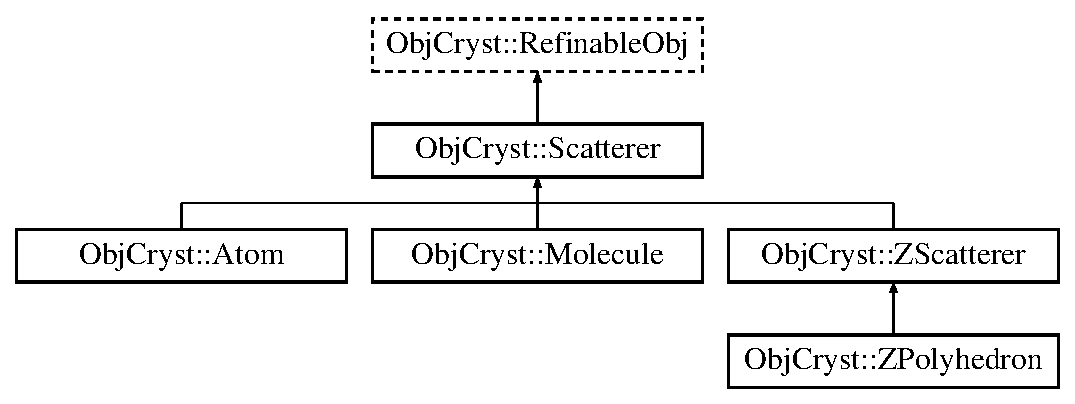
\includegraphics[height=2cm]{a00092}
\end{center}
\end{figure}
\subsubsection*{Public Member Functions}
\begin{DoxyCompactItemize}
\item 
{\bf SimplexObj} (const string name=\char`\"{}Unnamed Simplex Object\char`\"{})\label{a00092_a8af9110ac672b9b932adf838a853b90b}

\begin{DoxyCompactList}\small\item\em Constructor. \item\end{DoxyCompactList}\item 
virtual void {\bf Optimize} (long \&nbSteps, const bool silent=false, const REAL finalcost=0, const REAL maxTime=-\/1)
\begin{DoxyCompactList}\small\item\em Launch optimization (a single run) for N steps. \item\end{DoxyCompactList}\item 
virtual void {\bf MultiRunOptimize} (long \&nbCycle, long \&nbSteps, const bool silent=false, const REAL finalcost=0, const REAL maxTime=-\/1)
\begin{DoxyCompactList}\small\item\em Launch optimization for multiple runs of N steps. \item\end{DoxyCompactList}\item 
virtual void {\bf XMLOutput} (ostream \&os, int indent=0) const 
\begin{DoxyCompactList}\small\item\em Output a description of the object in XML format to a stream. \item\end{DoxyCompactList}\item 
virtual void {\bf XMLInput} (istream \&is, const {\bf XMLCrystTag} \&tag)
\begin{DoxyCompactList}\small\item\em Input in XML format from a stream, restoring the set of refined objects and the associated cost functions. \item\end{DoxyCompactList}\end{DoxyCompactItemize}
\subsubsection*{Private Member Functions}
\begin{DoxyCompactItemize}
\item 
REAL {\bf GenerateNewSimplexConfiguration} (CrystVector\_\-REAL \&vLLK, CrystVector\_\-long \&vIndex, unsigned long worst, REAL f)
\begin{DoxyCompactList}\small\item\em Try a new configuration by expanding the worst vertex from the center by a factor f. \item\end{DoxyCompactList}\end{DoxyCompactItemize}


\subsubsection{Detailed Description}
Conjugate Gradient Algorithm object. currently does not handle parameters hitting limits, and is not very efficient (uses numerical derivatives) 

\subsubsection{Member Function Documentation}
\index{ObjCryst::SimplexObj@{ObjCryst::SimplexObj}!GenerateNewSimplexConfiguration@{GenerateNewSimplexConfiguration}}
\index{GenerateNewSimplexConfiguration@{GenerateNewSimplexConfiguration}!ObjCryst::SimplexObj@{ObjCryst::SimplexObj}}
\paragraph[{GenerateNewSimplexConfiguration}]{\setlength{\rightskip}{0pt plus 5cm}REAL ObjCryst::SimplexObj::GenerateNewSimplexConfiguration (CrystVector\_\-REAL \& {\em vLLK}, \/  CrystVector\_\-long \& {\em vIndex}, \/  unsigned long {\em worst}, \/  REAL {\em f})\hspace{0.3cm}{\ttfamily  [private]}}\hfill\label{a00092_a5dbafc28130ee7db84587b8288c01830}


Try a new configuration by expanding the worst vertex from the center by a factor f. If it is better, store it as new worst. Return the new obtained llk \index{ObjCryst::SimplexObj@{ObjCryst::SimplexObj}!MultiRunOptimize@{MultiRunOptimize}}
\index{MultiRunOptimize@{MultiRunOptimize}!ObjCryst::SimplexObj@{ObjCryst::SimplexObj}}
\paragraph[{MultiRunOptimize}]{\setlength{\rightskip}{0pt plus 5cm}virtual void ObjCryst::SimplexObj::MultiRunOptimize (long \& {\em nbCycle}, \/  long \& {\em nbSteps}, \/  const bool {\em silent} = {\ttfamily false}, \/  const REAL {\em finalcost} = {\ttfamily 0}, \/  const REAL {\em maxTime} = {\ttfamily -\/1})\hspace{0.3cm}{\ttfamily  [virtual]}}\hfill\label{a00092_a1c7ae823f9e31169b453f36d15c049b8}


Launch optimization for multiple runs of N steps. 
\begin{DoxyParams}{Parameters}
\item[{\em nbCycle,:}]the number of runs (cycles) to perform. The structure is randomized at the beginning of each cycle. If nbCycle==-\/1, this will run indefinitely. The nbCycle parameter is decreased after each run. \item[{\em nbSteps,:}]the number of steps to go. This number is modified (decreases!) as the refinement goes on. \item[{\em silent}]: if true, absolutely no message should be printed (except debugging) \item[{\em finalcost,:}]the optimization will stop if overall cost fallse below this value \item[{\em maxTime,:}]the optimization will stop after the given number of seconds has been spent optimizing (ignored if $<$0). \end{DoxyParams}


Implements {\bf ObjCryst::OptimizationObj} \doxyref{}{p.}{a00054_aa53575dbda2ec3f561bed934beb4ca6f}.\index{ObjCryst::SimplexObj@{ObjCryst::SimplexObj}!Optimize@{Optimize}}
\index{Optimize@{Optimize}!ObjCryst::SimplexObj@{ObjCryst::SimplexObj}}
\paragraph[{Optimize}]{\setlength{\rightskip}{0pt plus 5cm}virtual void ObjCryst::SimplexObj::Optimize (long \& {\em nbSteps}, \/  const bool {\em silent} = {\ttfamily false}, \/  const REAL {\em finalcost} = {\ttfamily 0}, \/  const REAL {\em maxTime} = {\ttfamily -\/1})\hspace{0.3cm}{\ttfamily  [virtual]}}\hfill\label{a00092_aa8bf4b209e2ce6229722b18ec9911010}


Launch optimization (a single run) for N steps. 
\begin{DoxyParams}{Parameters}
\item[{\em nbSteps,:}]the number of steps to go. This number is modified (decreases!) as the refinement goes on. \item[{\em silent}]: if true, absolutely no message should be printed (except debugging) \item[{\em finalcost,:}]the optimization will stop if overall cost fallse below this value \item[{\em maxTime,:}]the optimization will stop after the given number of seconds has been spent optimizing (ignored if $<$0). \end{DoxyParams}


Implements {\bf ObjCryst::OptimizationObj} \doxyref{}{p.}{a00054_a08c77dc6ec80f63bf067ef2968a0b6dc}.\index{ObjCryst::SimplexObj@{ObjCryst::SimplexObj}!XMLInput@{XMLInput}}
\index{XMLInput@{XMLInput}!ObjCryst::SimplexObj@{ObjCryst::SimplexObj}}
\paragraph[{XMLInput}]{\setlength{\rightskip}{0pt plus 5cm}virtual void ObjCryst::SimplexObj::XMLInput (istream \& {\em is}, \/  const {\bf XMLCrystTag} \& {\em tag})\hspace{0.3cm}{\ttfamily  [virtual]}}\hfill\label{a00092_ae6ed0602ffdd2db1a10be80820a0a285}


Input in XML format from a stream, restoring the set of refined objects and the associated cost functions. Note that the corresponding objects must have been loaded in memory before, else shit happens. 

Implements {\bf ObjCryst::OptimizationObj} \doxyref{}{p.}{a00054_aa07aee60f56780e2c56fb20f4a5f48a8}.\index{ObjCryst::SimplexObj@{ObjCryst::SimplexObj}!XMLOutput@{XMLOutput}}
\index{XMLOutput@{XMLOutput}!ObjCryst::SimplexObj@{ObjCryst::SimplexObj}}
\paragraph[{XMLOutput}]{\setlength{\rightskip}{0pt plus 5cm}virtual void ObjCryst::SimplexObj::XMLOutput (ostream \& {\em os}, \/  int {\em indent} = {\ttfamily 0}) const\hspace{0.3cm}{\ttfamily  [virtual]}}\hfill\label{a00092_a7111042ca3a7201039a25fe548cb524c}


Output a description of the object in XML format to a stream. This saves the list of refined object and the cost functions, as well as options for the refinement. The refined objects are {\bfseries not} saved, so this must be done somewhere else (they must be reloaded before this object). 

Implements {\bf ObjCryst::OptimizationObj} \doxyref{}{p.}{a00054_a6b7726159bb0d5dad1c7eebaee78f53a}.

The documentation for this class was generated from the following file:\begin{DoxyCompactItemize}
\item 
Simplex.h\end{DoxyCompactItemize}

\subsection{ObjCryst::SpaceGroup::SMx Struct Reference}
\label{a00093}\index{ObjCryst::SpaceGroup::SMx@{ObjCryst::SpaceGroup::SMx}}


Struct to store rot+trans matrix.  
\subsubsection*{Public Attributes}
\begin{DoxyCompactItemize}
\item 
REAL {\bfseries mx} [9]\label{a00093_af1033aa35c50c8e536d1e656358b3580}

\item 
REAL {\bfseries tr} [3]\label{a00093_a1565a138ebe46589c74671c7037af97b}

\end{DoxyCompactItemize}


\subsubsection{Detailed Description}
Struct to store rot+trans matrix. 

The documentation for this struct was generated from the following file:\begin{DoxyCompactItemize}
\item 
SpaceGroup.h\end{DoxyCompactItemize}

\subsection{Obj\-Cryst\-:\-:Scattering\-Corr Class Reference}
\label{a00094}\index{Obj\-Cryst\-::\-Scattering\-Corr@{Obj\-Cryst\-::\-Scattering\-Corr}}


Base class to compute all kind of corrections to intensities\-: Lorentz, Polar, absorption, texcture, extinction, etc...  


Inheritance diagram for Obj\-Cryst\-:\-:Scattering\-Corr\-:\begin{figure}[H]
\begin{center}
\leavevmode
\includegraphics[height=1.056604cm]{a00094}
\end{center}
\end{figure}
\subsubsection*{Public Member Functions}
\begin{DoxyCompactItemize}
\item 
{\bf Scattering\-Corr} (const {\bf Scattering\-Data} \&data)\label{a00094_ac1e37a73b0a107f66d1b1d75b9db9c47}

\begin{DoxyCompactList}\small\item\em Constructor, with the associated \doxyref{Scattering\-Data}{p.}{a00095} object. \end{DoxyCompactList}\item 
virtual const string \& {\bf Get\-Name} () const =0\label{a00094_adb2782d4e32cbcb89e2e69b3c8ad66fb}

\begin{DoxyCompactList}\small\item\em Get the name of this object. \end{DoxyCompactList}\item 
virtual const string \& {\bf Get\-Class\-Name} () const =0\label{a00094_a6d72e7a6ffff0c16d86930d9e72c6673}

\begin{DoxyCompactList}\small\item\em Get the name of the class. \end{DoxyCompactList}\item 
const Cryst\-Vector\-\_\-\-R\-E\-A\-L \& {\bf Get\-Corr} () const 
\begin{DoxyCompactList}\small\item\em Get the vector of corrections for all reflections. \end{DoxyCompactList}\item 
const {\bf Refinable\-Obj\-Clock} \& {\bf Get\-Clock\-Corr} () const \label{a00094_a4c5bead3a47202db88495e3d123c5927}

\begin{DoxyCompactList}\small\item\em Get the value of the clock corresponding to the last time the correction was actually computed. \end{DoxyCompactList}\end{DoxyCompactItemize}
\subsubsection*{Protected Member Functions}
\begin{DoxyCompactItemize}
\item 
virtual void {\bf Calc\-Corr} () const =0\label{a00094_a437a916156f6d88c76cb01ca4c748c89}

\begin{DoxyCompactList}\small\item\em Do the computation of corrected intensities. \end{DoxyCompactList}\end{DoxyCompactItemize}
\subsubsection*{Protected Attributes}
\begin{DoxyCompactItemize}
\item 
const {\bf Scattering\-Data} $\ast$ {\bf mp\-Data}\label{a00094_a0fa066328104835ff72ddf98687c8513}

\begin{DoxyCompactList}\small\item\em The associated \doxyref{Scattering\-Data}{p.}{a00095} object. \end{DoxyCompactList}\item 
Cryst\-Vector\-\_\-\-R\-E\-A\-L {\bf m\-Corr}\label{a00094_a7669922ac4bbdfb826748148d4016088}

\begin{DoxyCompactList}\small\item\em The vector of correction to intensities. \end{DoxyCompactList}\item 
{\bf Refinable\-Obj\-Clock} {\bf m\-Clock\-Corr\-Calc}\label{a00094_aa969418138a9d1867797857318d6f303}

\begin{DoxyCompactList}\small\item\em The clock marking the last time the correction was calculated. \end{DoxyCompactList}\end{DoxyCompactItemize}


\subsubsection{Detailed Description}
Base class to compute all kind of corrections to intensities\-: Lorentz, Polar, absorption, texcture, extinction, etc... 

The computed intensities are to be multiplied by all the \doxyref{Scattering\-Corr}{p.}{a00094} calculated.

This is an abstract base class. 

\subsubsection{Member Function Documentation}
\index{Obj\-Cryst\-::\-Scattering\-Corr@{Obj\-Cryst\-::\-Scattering\-Corr}!Get\-Corr@{Get\-Corr}}
\index{Get\-Corr@{Get\-Corr}!ObjCryst::ScatteringCorr@{Obj\-Cryst\-::\-Scattering\-Corr}}
\paragraph[{Get\-Corr}]{\setlength{\rightskip}{0pt plus 5cm}const Cryst\-Vector\-\_\-\-R\-E\-A\-L\& Obj\-Cryst\-::\-Scattering\-Corr\-::\-Get\-Corr (
\begin{DoxyParamCaption}
{}
\end{DoxyParamCaption}
) const}\label{a00094_a50395369eb93155bf278453ba158f8cb}


Get the vector of corrections for all reflections. 

Calculated values must be multiplied by these values. 

The documentation for this class was generated from the following file\-:\begin{DoxyCompactItemize}
\item 
Scattering\-Corr.\-h\end{DoxyCompactItemize}

\subsection{ObjCryst::SpeedTestReport Struct Reference}
\label{a00095}\index{ObjCryst::SpeedTestReport@{ObjCryst::SpeedTestReport}}


Structure to hold the results of a speedtest (see \doxyref{ObjCryst::SpeedTest()}{p.}{a00170_a775b62d07c596365d2f2d021dca408db}).  
\subsubsection*{Public Attributes}
\begin{DoxyCompactItemize}
\item 
unsigned int {\bf mNbAtom}\label{a00095_a584ea20a9991658acac8f15ea6d2a670}

\begin{DoxyCompactList}\small\item\em Total number of unique atoms in the test structure. \item\end{DoxyCompactList}\item 
int {\bf mNbAtomType}\label{a00095_a755747dca57629b616b12341c110ff7e}

\begin{DoxyCompactList}\small\item\em Total number of atom types in the test structure. \item\end{DoxyCompactList}\item 
string {\bf mSpacegroup}\label{a00095_a73ae4759ba51ae06a745af9040398ccf}

\begin{DoxyCompactList}\small\item\em The symbol for the spacegroup. \item\end{DoxyCompactList}\item 
{\bf RadiationType} {\bf mRadiation}\label{a00095_a9407361e047413bd993828c9cfca4cdf}

\begin{DoxyCompactList}\small\item\em The type of radiation used. \item\end{DoxyCompactList}\item 
unsigned long {\bf mNbReflections}\label{a00095_a4fde54cf3f02e5f564df92cc8eabd36e}

\begin{DoxyCompactList}\small\item\em The total number of reflections used for the tests. \item\end{DoxyCompactList}\item 
unsigned int {\bf mDataType}\label{a00095_af3bb170b1d4ae3e1b484704b6c3d923c}

\begin{DoxyCompactList}\small\item\em dataType: 0= single crystal, 1= powder pattern (1 background + 1 crystal phase) \item\end{DoxyCompactList}\item 
REAL {\bf mBogoMRAPS}\label{a00095_ac7497f01fce186e1370bffdbc2f6433c}

\begin{DoxyCompactList}\small\item\em Million of Reflections-\/Atoms computed Per Second (considering all atoms in the unit cell). \item\end{DoxyCompactList}\item 
REAL {\bf mBogoMRAPS\_\-reduced}\label{a00095_a76d9645d24f787e53856512fbb918603}

\begin{DoxyCompactList}\small\item\em Million of Reflections-\/Atoms computed Per Second (considering all atoms in the unit cell, except those deduced by a center of symmetry or a lattice translation). \item\end{DoxyCompactList}\item 
REAL {\bf mBogoSPS}\label{a00095_ab45c0262f0cad316b2f3e8e74a8a5fd4}

\begin{DoxyCompactList}\small\item\em Number of Structures evaluated Per Second. \item\end{DoxyCompactList}\end{DoxyCompactItemize}


\subsubsection{Detailed Description}
Structure to hold the results of a speedtest (see \doxyref{ObjCryst::SpeedTest()}{p.}{a00170_a775b62d07c596365d2f2d021dca408db}). 

The documentation for this struct was generated from the following file:\begin{DoxyCompactItemize}
\item 
test.h\end{DoxyCompactItemize}

\subsection{\-Obj\-Cryst\-:\-:\-Speed\-Test\-Report \-Struct \-Reference}
\label{a00096}\index{\-Obj\-Cryst\-::\-Speed\-Test\-Report@{\-Obj\-Cryst\-::\-Speed\-Test\-Report}}


\-Structure to hold the results of a speedtest (see \doxyref{\-Obj\-Cryst\-::\-Speed\-Test()}{p.}{a00171_a775b62d07c596365d2f2d021dca408db})  


\subsubsection*{\-Public \-Attributes}
\begin{DoxyCompactItemize}
\item 
unsigned int {\bf m\-Nb\-Atom}\label{a00096_a584ea20a9991658acac8f15ea6d2a670}

\begin{DoxyCompactList}\small\item\em \-Total number of unique atoms in the test structure. \end{DoxyCompactList}\item 
int {\bf m\-Nb\-Atom\-Type}\label{a00096_a755747dca57629b616b12341c110ff7e}

\begin{DoxyCompactList}\small\item\em \-Total number of atom types in the test structure. \end{DoxyCompactList}\item 
string {\bf m\-Spacegroup}\label{a00096_a73ae4759ba51ae06a745af9040398ccf}

\begin{DoxyCompactList}\small\item\em \-The symbol for the spacegroup. \end{DoxyCompactList}\item 
{\bf \-Radiation\-Type} {\bf m\-Radiation}\label{a00096_a9407361e047413bd993828c9cfca4cdf}

\begin{DoxyCompactList}\small\item\em \-The type of radiation used. \end{DoxyCompactList}\item 
unsigned long {\bf m\-Nb\-Reflections}\label{a00096_a4fde54cf3f02e5f564df92cc8eabd36e}

\begin{DoxyCompactList}\small\item\em \-The total number of reflections used for the tests. \end{DoxyCompactList}\item 
unsigned int {\bf m\-Data\-Type}\label{a00096_af3bb170b1d4ae3e1b484704b6c3d923c}

\begin{DoxyCompactList}\small\item\em data\-Type\-: 0= single crystal, 1= powder pattern (1 background + 1 crystal phase) \end{DoxyCompactList}\item 
\-R\-E\-A\-L {\bf m\-Bogo\-M\-R\-A\-P\-S}\label{a00096_ac7497f01fce186e1370bffdbc2f6433c}

\begin{DoxyCompactList}\small\item\em \-Million of \-Reflections-\/\-Atoms computed \-Per \-Second (considering all atoms in the unit cell) \end{DoxyCompactList}\item 
\-R\-E\-A\-L {\bf m\-Bogo\-M\-R\-A\-P\-S\-\_\-reduced}\label{a00096_a76d9645d24f787e53856512fbb918603}

\begin{DoxyCompactList}\small\item\em \-Million of \-Reflections-\/\-Atoms computed \-Per \-Second (considering all atoms in the unit cell, except those deduced by a center of symmetry or a lattice translation) \end{DoxyCompactList}\item 
\-R\-E\-A\-L {\bf m\-Bogo\-S\-P\-S}\label{a00096_ab45c0262f0cad316b2f3e8e74a8a5fd4}

\begin{DoxyCompactList}\small\item\em \-Number of \-Structures evaluated \-Per \-Second. \end{DoxyCompactList}\end{DoxyCompactItemize}


\subsubsection{\-Detailed \-Description}
\-Structure to hold the results of a speedtest (see \doxyref{\-Obj\-Cryst\-::\-Speed\-Test()}{p.}{a00171_a775b62d07c596365d2f2d021dca408db}) 



\-The documentation for this struct was generated from the following file\-:\begin{DoxyCompactItemize}
\item 
test.\-h\end{DoxyCompactItemize}

\subsection{Obj\-Cryst\-:\-:Stretch\-Mode Struct Reference}
\label{a00097}\index{Obj\-Cryst\-::\-Stretch\-Mode@{Obj\-Cryst\-::\-Stretch\-Mode}}


Abstract base Stretch Mode for \doxyref{Molecule}{p.}{a00047} objects.  


Inheritance diagram for Obj\-Cryst\-:\-:Stretch\-Mode\-:\begin{figure}[H]
\begin{center}
\leavevmode
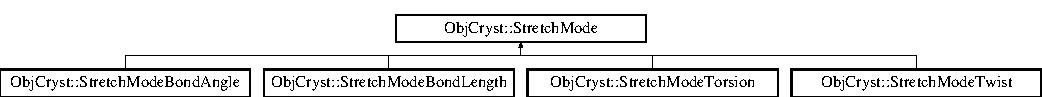
\includegraphics[height=1.302326cm]{a00097}
\end{center}
\end{figure}
\subsubsection*{Public Member Functions}
\begin{DoxyCompactItemize}
\item 
virtual void {\bf Calc\-Deriv} (const bool derivllk=true) const =0
\begin{DoxyCompactList}\small\item\em Calculate the derivative of the \doxyref{Molecule}{p.}{a00047}'s Log(likelihood) and atomic positions versus a change of the bond length. \end{DoxyCompactList}\item 
virtual void {\bf Print} (ostream \&os, bool full=true) const =0\label{a00097_a78c180042fce5981fe0e97071d986362}

\begin{DoxyCompactList}\small\item\em Print one-\/line list of atoms moved. \end{DoxyCompactList}\item 
virtual void {\bf Stretch} (const R\-E\-A\-L change)=0\label{a00097_a1f3e7e8fc43baed619b61203ea77c143}

\begin{DoxyCompactList}\small\item\em Move the atoms according to this mode. \end{DoxyCompactList}\item 
virtual void {\bf Random\-Stretch} (const R\-E\-A\-L amplitude)=0\label{a00097_a459057c6cd3d2cb1010676b54ebfe988}

\begin{DoxyCompactList}\small\item\em Move the atoms according to this mode, randomly. \end{DoxyCompactList}\end{DoxyCompactItemize}
\subsubsection*{Public Attributes}
\begin{DoxyCompactItemize}
\item 
std\-::map$<$ const {\bf Mol\-Bond} $\ast$, R\-E\-A\-L $>$ {\bf mvp\-Broken\-Bond}\label{a00097_a6628812c69f20a7a18a7a3759b5c961c}

\begin{DoxyCompactList}\small\item\em List of bond restraints affected by this mode The key is the restraint, the value is the derivative of the L\-L\-K associated. \end{DoxyCompactList}\item 
std\-::map$<$ const {\bf Mol\-Bond\-Angle} \\*
$\ast$, R\-E\-A\-L $>$ {\bf mvp\-Broken\-Bond\-Angle}\label{a00097_a2a46f6bd997850be6736e4b5746deeed}

\begin{DoxyCompactList}\small\item\em List of bond angle restraints modified by this mode The key is the restraint, the value is the derivative of the L\-L\-K associated. \end{DoxyCompactList}\item 
std\-::map$<$ const \\*
{\bf Mol\-Dihedral\-Angle} $\ast$, R\-E\-A\-L $>$ {\bf mvp\-Broken\-Dihedral\-Angle}\label{a00097_a84257bc829a3d612b68046d33685e59e}

\begin{DoxyCompactList}\small\item\em List of dihedral angle restraints modified by this mode The key is the restraint, the value is the derivative of the L\-L\-K associated. \end{DoxyCompactList}\item 
R\-E\-A\-L {\bf m\-L\-L\-K\-Deriv}\label{a00097_ac6614921c015de3f6d67b22ae512a66c}

\begin{DoxyCompactList}\small\item\em Derivative of the \doxyref{Molecule}{p.}{a00047}'s Log(likelihood) versus a change of the bond length. \end{DoxyCompactList}\item 
std\-::map$<$ const {\bf Mol\-Atom} $\ast$, {\bf X\-Y\-Z} $>$ {\bf m\-Deriv\-X\-Y\-Z}\label{a00097_a4a25093e177c56be142acc954149c110}

\begin{DoxyCompactList}\small\item\em Derivative of the atomic positions versus a change of the bond length. \end{DoxyCompactList}\item 
{\bf Molecule} $\ast$ {\bf mp\-Mol}\label{a00097_a380bd0aef1e5be1f681364e0f754f3e3}

\begin{DoxyCompactList}\small\item\em The \doxyref{Molecule}{p.}{a00047} corresponding to this stretch mode. \end{DoxyCompactList}\item 
R\-E\-A\-L {\bf m\-Base\-Amplitude}
\begin{DoxyCompactList}\small\item\em The recommended change amplitude, for a base global optimization displacement, to obtain an average 0.\-1 Angstroem displacement. \end{DoxyCompactList}\end{DoxyCompactItemize}


\subsubsection{Detailed Description}
Abstract base Stretch Mode for \doxyref{Molecule}{p.}{a00047} objects. 



\subsubsection{Member Function Documentation}
\index{Obj\-Cryst\-::\-Stretch\-Mode@{Obj\-Cryst\-::\-Stretch\-Mode}!Calc\-Deriv@{Calc\-Deriv}}
\index{Calc\-Deriv@{Calc\-Deriv}!ObjCryst::StretchMode@{Obj\-Cryst\-::\-Stretch\-Mode}}
\paragraph[{Calc\-Deriv}]{\setlength{\rightskip}{0pt plus 5cm}virtual void Obj\-Cryst\-::\-Stretch\-Mode\-::\-Calc\-Deriv (
\begin{DoxyParamCaption}
\item[{const bool}]{derivllk = {\ttfamily true}}
\end{DoxyParamCaption}
) const\hspace{0.3cm}{\ttfamily [pure virtual]}}\label{a00097_a5b5ab5f9819c047a49719a330722d419}


Calculate the derivative of the \doxyref{Molecule}{p.}{a00047}'s Log(likelihood) and atomic positions versus a change of the bond length. 

The result is stored in m\-L\-L\-K\-Deriv and m\-L\-L\-K\-Deriv\-X\-Y\-Z, as well as in the various lists of restraints broken by this mode.


\begin{DoxyParams}{Parameters}
{\em derivllk,\-:} & if false, the derivative of the overall llk will not be computed, only the derivative of the atomic positions. \\
\hline
\end{DoxyParams}


Implemented in {\bf Obj\-Cryst\-::\-Stretch\-Mode\-Twist} \doxyref{}{p.}{a00102_afd1ac754d10507e1c9bed829a4eaeb79}, {\bf Obj\-Cryst\-::\-Stretch\-Mode\-Torsion} \doxyref{}{p.}{a00101_abecf1074b05ba13fd938667399df110e}, {\bf Obj\-Cryst\-::\-Stretch\-Mode\-Bond\-Angle} \doxyref{}{p.}{a00098_acdc082c4cb5b4f38fed6049bf7b1eb9c}, and {\bf Obj\-Cryst\-::\-Stretch\-Mode\-Bond\-Length} \doxyref{}{p.}{a00099_a72bab02ebf84cbf65cf2703e74c1e02e}.



\subsubsection{Member Data Documentation}
\index{Obj\-Cryst\-::\-Stretch\-Mode@{Obj\-Cryst\-::\-Stretch\-Mode}!m\-Base\-Amplitude@{m\-Base\-Amplitude}}
\index{m\-Base\-Amplitude@{m\-Base\-Amplitude}!ObjCryst::StretchMode@{Obj\-Cryst\-::\-Stretch\-Mode}}
\paragraph[{m\-Base\-Amplitude}]{\setlength{\rightskip}{0pt plus 5cm}R\-E\-A\-L Obj\-Cryst\-::\-Stretch\-Mode\-::m\-Base\-Amplitude}\label{a00097_aa8dc03e2bd6840d13964dd6751c39fae}


The recommended change amplitude, for a base global optimization displacement, to obtain an average 0.\-1 Angstroem displacement. 

This is learnt at the beginning of an optimization.

This can be superseeded to respect any restraint. 

The documentation for this struct was generated from the following file\-:\begin{DoxyCompactItemize}
\item 
Molecule.\-h\end{DoxyCompactItemize}

\subsection{\-Obj\-Cryst\-:\-:\-Stretch\-Mode\-Bond\-Angle \-Struct \-Reference}
\label{a00098}\index{\-Obj\-Cryst\-::\-Stretch\-Mode\-Bond\-Angle@{\-Obj\-Cryst\-::\-Stretch\-Mode\-Bond\-Angle}}


\-Atoms moved when changing a bond angle.  


\-Inheritance diagram for \-Obj\-Cryst\-:\-:\-Stretch\-Mode\-Bond\-Angle\-:\begin{figure}[H]
\begin{center}
\leavevmode
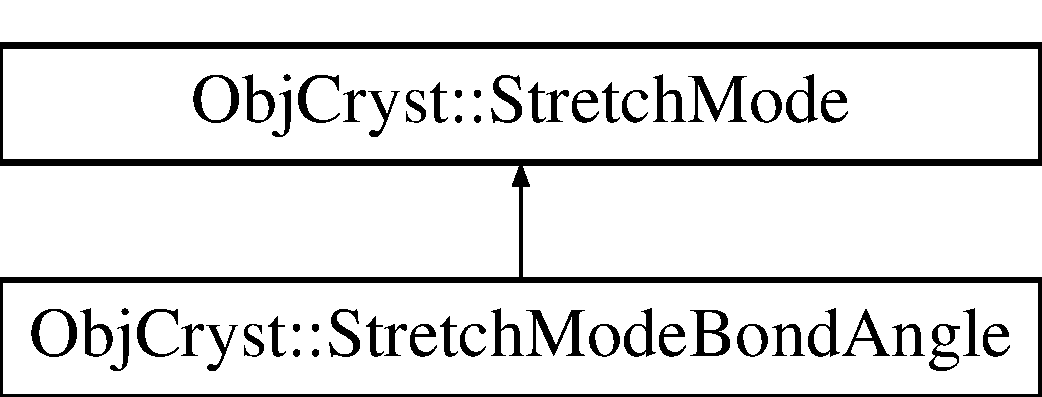
\includegraphics[height=2.000000cm]{a00098}
\end{center}
\end{figure}
\subsubsection*{\-Public \-Member \-Functions}
\begin{DoxyCompactItemize}
\item 
{\bf \-Stretch\-Mode\-Bond\-Angle} ({\bf \-Mol\-Atom} \&at0, {\bf \-Mol\-Atom} \&at1, {\bf \-Mol\-Atom} \&at2, const {\bf \-Mol\-Bond\-Angle} $\ast$p\-Bond\-Angle)\label{a00098_aa1fbf3238722b663b083c999cf1b5c57}

\begin{DoxyCompactList}\small\item\em \-Constructor \-If p\-Bond\-Angle!=0, the bond angle length restraint is respected. \end{DoxyCompactList}\item 
virtual void {\bf \-Calc\-Deriv} (const bool derivllk=true) const 
\begin{DoxyCompactList}\small\item\em \-Calculate the derivative of the \doxyref{\-Molecule}{p.}{a00047}'s \-Log(likelihood) and atomic positions versus a change of the bond length. \end{DoxyCompactList}\item 
virtual void {\bf \-Print} (ostream \&os, bool full=true) const \label{a00098_a77e72910a64e3351a05a2f7ac47033c0}

\begin{DoxyCompactList}\small\item\em \-Print one-\/line list of atoms moved. \end{DoxyCompactList}\item 
virtual void {\bf \-Stretch} (const \-R\-E\-A\-L change)\label{a00098_aff6934e2b0a048d164228348f87f544d}

\begin{DoxyCompactList}\small\item\em \-Move the atoms according to this mode. \end{DoxyCompactList}\item 
virtual void {\bf \-Random\-Stretch} (const \-R\-E\-A\-L amplitude)\label{a00098_a7e3006f5ecd0d683ec669475c5f21394}

\begin{DoxyCompactList}\small\item\em \-Move the atoms according to this mode, randomly. \end{DoxyCompactList}\end{DoxyCompactItemize}
\subsubsection*{\-Public \-Attributes}
\begin{DoxyCompactItemize}
\item 
{\bf \-Mol\-Atom} $\ast$ {\bf mp\-Atom0}\label{a00098_a63bc5bb54f0d298fb47b7bf86e8c2ff5}

\begin{DoxyCompactList}\small\item\em \-The first atom. \end{DoxyCompactList}\item 
{\bf \-Mol\-Atom} $\ast$ {\bf mp\-Atom1}\label{a00098_aa5b52fcece40cd41c93eeb8b1dfec939}

\begin{DoxyCompactList}\small\item\em \-The second atom. \end{DoxyCompactList}\item 
{\bf \-Mol\-Atom} $\ast$ {\bf mp\-Atom2}\label{a00098_a08c6b4fde05610d0242bfd7b4a6acc3f}

\begin{DoxyCompactList}\small\item\em \-The third atom. \end{DoxyCompactList}\item 
const {\bf \-Mol\-Bond\-Angle} $\ast$ {\bf mp\-Bond\-Angle}\label{a00098_ab173d155feb360d0b95b5cd35f346da5}

\begin{DoxyCompactList}\small\item\em \-The (optional) bond angle restraint which this stretch mode should respect. \end{DoxyCompactList}\item 
set$<$ {\bf \-Mol\-Atom} $\ast$ $>$ {\bf mv\-Rotated\-Atom\-List}
\begin{DoxyCompactList}\small\item\em \-The set of atoms that are to be rotated around the direction going through at1 and perpendicular to the at0-\/at1-\/at2 plane. \end{DoxyCompactList}\end{DoxyCompactItemize}


\subsubsection{\-Detailed \-Description}
\-Atoms moved when changing a bond angle. 

\-This should be merged (or have an inheritance relation) with \doxyref{\-Mol\-Bond\-Angle}{p.}{a00045}. 

\subsubsection{\-Member \-Function \-Documentation}
\index{\-Obj\-Cryst\-::\-Stretch\-Mode\-Bond\-Angle@{\-Obj\-Cryst\-::\-Stretch\-Mode\-Bond\-Angle}!\-Calc\-Deriv@{\-Calc\-Deriv}}
\index{\-Calc\-Deriv@{\-Calc\-Deriv}!ObjCryst::StretchModeBondAngle@{\-Obj\-Cryst\-::\-Stretch\-Mode\-Bond\-Angle}}
\paragraph[{\-Calc\-Deriv}]{\setlength{\rightskip}{0pt plus 5cm}virtual void {\bf \-Obj\-Cryst\-::\-Stretch\-Mode\-Bond\-Angle\-::\-Calc\-Deriv} (
\begin{DoxyParamCaption}
\item[{const bool}]{derivllk = {\ttfamily true}}
\end{DoxyParamCaption}
) const\hspace{0.3cm}{\ttfamily  [virtual]}}\label{a00098_acdc082c4cb5b4f38fed6049bf7b1eb9c}


\-Calculate the derivative of the \doxyref{\-Molecule}{p.}{a00047}'s \-Log(likelihood) and atomic positions versus a change of the bond length. 

\-The result is stored in m\-L\-L\-K\-Deriv and m\-L\-L\-K\-Deriv\-X\-Y\-Z, as well as in the various lists of restraints broken by this mode.


\begin{DoxyParams}{\-Parameters}
{\em derivllk,\-:} & if false, the derivative of the overall llk will not be computed, only the derivative of the atomic positions. \\
\hline
\end{DoxyParams}


\-Implements {\bf \-Obj\-Cryst\-::\-Stretch\-Mode} \doxyref{}{p.}{a00097_a5b5ab5f9819c047a49719a330722d419}.



\subsubsection{\-Member \-Data \-Documentation}
\index{\-Obj\-Cryst\-::\-Stretch\-Mode\-Bond\-Angle@{\-Obj\-Cryst\-::\-Stretch\-Mode\-Bond\-Angle}!mv\-Rotated\-Atom\-List@{mv\-Rotated\-Atom\-List}}
\index{mv\-Rotated\-Atom\-List@{mv\-Rotated\-Atom\-List}!ObjCryst::StretchModeBondAngle@{\-Obj\-Cryst\-::\-Stretch\-Mode\-Bond\-Angle}}
\paragraph[{mv\-Rotated\-Atom\-List}]{\setlength{\rightskip}{0pt plus 5cm}set$<${\bf \-Mol\-Atom} $\ast$$>$ {\bf \-Obj\-Cryst\-::\-Stretch\-Mode\-Bond\-Angle\-::mv\-Rotated\-Atom\-List}}\label{a00098_a1d70964f33ea3a594efd2c3a595816a6}


\-The set of atoms that are to be rotated around the direction going through at1 and perpendicular to the at0-\/at1-\/at2 plane. 



\-The documentation for this struct was generated from the following file\-:\begin{DoxyCompactItemize}
\item 
\-Molecule.\-h\end{DoxyCompactItemize}

\subsection{Obj\+Cryst\+:\+:Simplex\+Obj Class Reference}
\label{a00099}\index{Obj\+Cryst\+::\+Simplex\+Obj@{Obj\+Cryst\+::\+Simplex\+Obj}}


Conjugate Gradient Algorithm object.  


Inheritance diagram for Obj\+Cryst\+:\+:Simplex\+Obj\+:\begin{figure}[H]
\begin{center}
\leavevmode
\includegraphics[height=2.000000cm]{a00099}
\end{center}
\end{figure}
\subsubsection*{Public Member Functions}
\begin{DoxyCompactItemize}
\item 
{\bf Simplex\+Obj} (const string name=\char`\"{}Unnamed Simplex Object\char`\"{})\label{a00099_a8af9110ac672b9b932adf838a853b90b}

\begin{DoxyCompactList}\small\item\em Constructor. \end{DoxyCompactList}\item 
virtual void {\bf Optimize} (long \&nb\+Steps, const bool silent=false, const R\+E\+A\+L finalcost=0, const R\+E\+A\+L max\+Time=-\/1)
\begin{DoxyCompactList}\small\item\em Launch optimization (a single run) for N steps. \end{DoxyCompactList}\item 
virtual void {\bf Multi\+Run\+Optimize} (long \&nb\+Cycle, long \&nb\+Steps, const bool silent=false, const R\+E\+A\+L finalcost=0, const R\+E\+A\+L max\+Time=-\/1)
\begin{DoxyCompactList}\small\item\em Launch optimization for multiple runs of N steps. \end{DoxyCompactList}\item 
virtual void {\bf X\+M\+L\+Output} (ostream \&os, int indent=0) const 
\begin{DoxyCompactList}\small\item\em Output a description of the object in X\+M\+L format to a stream. \end{DoxyCompactList}\item 
virtual void {\bf X\+M\+L\+Input} (istream \&is, const {\bf X\+M\+L\+Cryst\+Tag} \&tag)
\begin{DoxyCompactList}\small\item\em Input in X\+M\+L format from a stream, restoring the set of refined objects and the associated cost functions. \end{DoxyCompactList}\end{DoxyCompactItemize}
\subsubsection*{Private Member Functions}
\begin{DoxyCompactItemize}
\item 
R\+E\+A\+L {\bf Generate\+New\+Simplex\+Configuration} (Cryst\+Vector\+\_\+\+R\+E\+A\+L \&v\+L\+L\+K, Cryst\+Vector\+\_\+long \&v\+Index, unsigned long worst, R\+E\+A\+L f)
\begin{DoxyCompactList}\small\item\em Try a new configuration by expanding the worst vertex from the center by a factor f. \end{DoxyCompactList}\end{DoxyCompactItemize}
\subsubsection*{Additional Inherited Members}


\subsubsection{Detailed Description}
Conjugate Gradient Algorithm object. 

currently does not handle parameters hitting limits, and is not very efficient (uses numerical derivatives) 

\subsubsection{Member Function Documentation}
\index{Obj\+Cryst\+::\+Simplex\+Obj@{Obj\+Cryst\+::\+Simplex\+Obj}!Generate\+New\+Simplex\+Configuration@{Generate\+New\+Simplex\+Configuration}}
\index{Generate\+New\+Simplex\+Configuration@{Generate\+New\+Simplex\+Configuration}!Obj\+Cryst\+::\+Simplex\+Obj@{Obj\+Cryst\+::\+Simplex\+Obj}}
\paragraph[{Generate\+New\+Simplex\+Configuration}]{\setlength{\rightskip}{0pt plus 5cm}R\+E\+A\+L Obj\+Cryst\+::\+Simplex\+Obj\+::\+Generate\+New\+Simplex\+Configuration (
\begin{DoxyParamCaption}
\item[{Cryst\+Vector\+\_\+\+R\+E\+A\+L \&}]{v\+L\+L\+K, }
\item[{Cryst\+Vector\+\_\+long \&}]{v\+Index, }
\item[{unsigned long}]{worst, }
\item[{R\+E\+A\+L}]{f}
\end{DoxyParamCaption}
)\hspace{0.3cm}{\ttfamily [private]}}\label{a00099_a5dbafc28130ee7db84587b8288c01830}


Try a new configuration by expanding the worst vertex from the center by a factor f. 

If it is better, store it as new worst. Return the new obtained llk \index{Obj\+Cryst\+::\+Simplex\+Obj@{Obj\+Cryst\+::\+Simplex\+Obj}!Multi\+Run\+Optimize@{Multi\+Run\+Optimize}}
\index{Multi\+Run\+Optimize@{Multi\+Run\+Optimize}!Obj\+Cryst\+::\+Simplex\+Obj@{Obj\+Cryst\+::\+Simplex\+Obj}}
\paragraph[{Multi\+Run\+Optimize}]{\setlength{\rightskip}{0pt plus 5cm}virtual void Obj\+Cryst\+::\+Simplex\+Obj\+::\+Multi\+Run\+Optimize (
\begin{DoxyParamCaption}
\item[{long \&}]{nb\+Cycle, }
\item[{long \&}]{nb\+Steps, }
\item[{const bool}]{silent = {\ttfamily false}, }
\item[{const R\+E\+A\+L}]{finalcost = {\ttfamily 0}, }
\item[{const R\+E\+A\+L}]{max\+Time = {\ttfamily -\/1}}
\end{DoxyParamCaption}
)\hspace{0.3cm}{\ttfamily [virtual]}}\label{a00099_a1c7ae823f9e31169b453f36d15c049b8}


Launch optimization for multiple runs of N steps. 


\begin{DoxyParams}{Parameters}
{\em nb\+Cycle} & the number of runs (cycles) to perform. The structure is randomized at the beginning of each cycle. If nb\+Cycle==-\/1, this will run indefinitely. The nb\+Cycle parameter is decreased after each run. \\
\hline
{\em nb\+Steps} & the number of steps to go. This number is modified (decreases!) as the refinement goes on. \\
\hline
{\em silent} & \+: if true, absolutely no message should be printed (except debugging) \\
\hline
{\em finalcost} & the optimization will stop if overall cost fallse below this value \\
\hline
{\em max\+Time} & the optimization will stop after the given number of seconds has been spent optimizing (ignored if $<$0). \\
\hline
\end{DoxyParams}


Implements {\bf Obj\+Cryst\+::\+Optimization\+Obj} \doxyref{}{p.}{a00061_aa53575dbda2ec3f561bed934beb4ca6f}.

\index{Obj\+Cryst\+::\+Simplex\+Obj@{Obj\+Cryst\+::\+Simplex\+Obj}!Optimize@{Optimize}}
\index{Optimize@{Optimize}!Obj\+Cryst\+::\+Simplex\+Obj@{Obj\+Cryst\+::\+Simplex\+Obj}}
\paragraph[{Optimize}]{\setlength{\rightskip}{0pt plus 5cm}virtual void Obj\+Cryst\+::\+Simplex\+Obj\+::\+Optimize (
\begin{DoxyParamCaption}
\item[{long \&}]{nb\+Steps, }
\item[{const bool}]{silent = {\ttfamily false}, }
\item[{const R\+E\+A\+L}]{finalcost = {\ttfamily 0}, }
\item[{const R\+E\+A\+L}]{max\+Time = {\ttfamily -\/1}}
\end{DoxyParamCaption}
)\hspace{0.3cm}{\ttfamily [virtual]}}\label{a00099_aa8bf4b209e2ce6229722b18ec9911010}


Launch optimization (a single run) for N steps. 


\begin{DoxyParams}{Parameters}
{\em nb\+Steps} & the number of steps to go. This number is modified (decreases!) as the refinement goes on. \\
\hline
{\em silent} & \+: if true, absolutely no message should be printed (except debugging) \\
\hline
{\em finalcost} & the optimization will stop if overall cost fallse below this value \\
\hline
{\em max\+Time} & the optimization will stop after the given number of seconds has been spent optimizing (ignored if $<$0). \\
\hline
\end{DoxyParams}


Implements {\bf Obj\+Cryst\+::\+Optimization\+Obj} \doxyref{}{p.}{a00061_a08c77dc6ec80f63bf067ef2968a0b6dc}.

\index{Obj\+Cryst\+::\+Simplex\+Obj@{Obj\+Cryst\+::\+Simplex\+Obj}!X\+M\+L\+Input@{X\+M\+L\+Input}}
\index{X\+M\+L\+Input@{X\+M\+L\+Input}!Obj\+Cryst\+::\+Simplex\+Obj@{Obj\+Cryst\+::\+Simplex\+Obj}}
\paragraph[{X\+M\+L\+Input}]{\setlength{\rightskip}{0pt plus 5cm}virtual void Obj\+Cryst\+::\+Simplex\+Obj\+::\+X\+M\+L\+Input (
\begin{DoxyParamCaption}
\item[{istream \&}]{is, }
\item[{const {\bf X\+M\+L\+Cryst\+Tag} \&}]{tag}
\end{DoxyParamCaption}
)\hspace{0.3cm}{\ttfamily [virtual]}}\label{a00099_ae6ed0602ffdd2db1a10be80820a0a285}


Input in X\+M\+L format from a stream, restoring the set of refined objects and the associated cost functions. 

Note that the corresponding objects must have been loaded in memory before, else shit happens. 

Implements {\bf Obj\+Cryst\+::\+Optimization\+Obj} \doxyref{}{p.}{a00061_aa07aee60f56780e2c56fb20f4a5f48a8}.

\index{Obj\+Cryst\+::\+Simplex\+Obj@{Obj\+Cryst\+::\+Simplex\+Obj}!X\+M\+L\+Output@{X\+M\+L\+Output}}
\index{X\+M\+L\+Output@{X\+M\+L\+Output}!Obj\+Cryst\+::\+Simplex\+Obj@{Obj\+Cryst\+::\+Simplex\+Obj}}
\paragraph[{X\+M\+L\+Output}]{\setlength{\rightskip}{0pt plus 5cm}virtual void Obj\+Cryst\+::\+Simplex\+Obj\+::\+X\+M\+L\+Output (
\begin{DoxyParamCaption}
\item[{ostream \&}]{os, }
\item[{int}]{indent = {\ttfamily 0}}
\end{DoxyParamCaption}
) const\hspace{0.3cm}{\ttfamily [virtual]}}\label{a00099_a7111042ca3a7201039a25fe548cb524c}


Output a description of the object in X\+M\+L format to a stream. 

This saves the list of refined object and the cost functions, as well as options for the refinement. The refined objects are {\bfseries not} saved, so this must be done somewhere else (they must be reloaded before this object). 

Implements {\bf Obj\+Cryst\+::\+Optimization\+Obj} \doxyref{}{p.}{a00061_a6b7726159bb0d5dad1c7eebaee78f53a}.



The documentation for this class was generated from the following file\+:\begin{DoxyCompactItemize}
\item 
Simplex.\+h\end{DoxyCompactItemize}

\subsection{Obj\+Cryst\+:\+:Space\+Group\+:\+:S\+Mx Struct Reference}
\label{a00100}\index{Obj\+Cryst\+::\+Space\+Group\+::\+S\+Mx@{Obj\+Cryst\+::\+Space\+Group\+::\+S\+Mx}}


Struct to store rot+trans matrix.  


\subsubsection*{Public Attributes}
\begin{DoxyCompactItemize}
\item 
R\+E\+A\+L {\bfseries mx} [9]\label{a00100_af1033aa35c50c8e536d1e656358b3580}

\item 
R\+E\+A\+L {\bfseries tr} [3]\label{a00100_a1565a138ebe46589c74671c7037af97b}

\end{DoxyCompactItemize}


\subsubsection{Detailed Description}
Struct to store rot+trans matrix. 

The documentation for this struct was generated from the following file\+:\begin{DoxyCompactItemize}
\item 
Space\+Group.\+h\end{DoxyCompactItemize}

\subsection{Obj\+Cryst\+:\+:Space\+Group Class Reference}
\label{a00101}\index{Obj\+Cryst\+::\+Space\+Group@{Obj\+Cryst\+::\+Space\+Group}}


The crystallographic space group, and the cell choice.  


\subsubsection*{Classes}
\begin{DoxyCompactItemize}
\item 
struct {\bf S\+Mx}
\begin{DoxyCompactList}\small\item\em Struct to store rot+trans matrix. \end{DoxyCompactList}\item 
struct {\bf T\+Rx}
\begin{DoxyCompactList}\small\item\em Struct to store trans matrix. \end{DoxyCompactList}\end{DoxyCompactItemize}
\subsubsection*{Public Member Functions}
\begin{DoxyCompactItemize}
\item 
{\bf Space\+Group} ()
\begin{DoxyCompactList}\small\item\em Default Constructor (initializes in P1) \end{DoxyCompactList}\item 
{\bf Space\+Group} (const string \&spg\+Id)
\begin{DoxyCompactList}\small\item\em Constructor with a specified spacegroup symbol or number. \end{DoxyCompactList}\item 
{\bf $\sim$\+Space\+Group} ()\label{a00101_a9dfc390a5e455426c323ee7a8d6ced10}

\begin{DoxyCompactList}\small\item\em Destructor. \end{DoxyCompactList}\item 
void {\bf Change\+Space\+Group} (const string \&spg\+Id)\label{a00101_af592aa42f04d02e4caecbf2b93031be8}

\begin{DoxyCompactList}\small\item\em Change the Spacegroup. \end{DoxyCompactList}\item 
const string \& {\bf Get\+Name} () const \label{a00101_a633e6ba97400f7b4f7d3887c94dce2c0}

\begin{DoxyCompactList}\small\item\em Get the name of this spacegroup (its name, as supplied initially by the calling program or user) \end{DoxyCompactList}\item 
bool {\bf Is\+In\+Asymmetric\+Unit} (const R\+E\+A\+L x, const R\+E\+A\+L y, const R\+E\+A\+L z) const \label{a00101_accd8f865d9cbb12e420a6737fe50bc06}

\begin{DoxyCompactList}\small\item\em Test if a given scatterer at (x,y,z) is in the asymmetric unit. \end{DoxyCompactList}\item 
void {\bf Change\+To\+Asymmetric\+Unit} (R\+E\+A\+L x, R\+E\+A\+L y, R\+E\+A\+L z) const 
\begin{DoxyCompactList}\small\item\em Move (x,y,z) coordinates to their equivalent in the asym unit. \end{DoxyCompactList}\item 
const {\bf Asymmetric\+Unit} \& {\bf Get\+Asym\+Unit} () const \label{a00101_aaf14567efef1b6031df146a3f8b7b9a2}

\begin{DoxyCompactList}\small\item\em Get the \doxyref{Asymmetric\+Unit}{p.}{a00013} for this spacegroup. \end{DoxyCompactList}\item 
int {\bf Get\+Space\+Group\+Number} () const \label{a00101_add04f45fac118cc9c235a6a6270d12c7}

\begin{DoxyCompactList}\small\item\em Id number of the spacegroup. \end{DoxyCompactList}\item 
bool {\bf Is\+Centrosymmetric} () const \label{a00101_a0f2bc9f6351fcde894338cad26d5617e}

\begin{DoxyCompactList}\small\item\em Is the crystal centrosymmetric ? \end{DoxyCompactList}\item 
int {\bf Get\+Nb\+Translation\+Vectors} () const 
\begin{DoxyCompactList}\small\item\em Number of translation vectors (1 for 'P' cells, 2 for 'I', 4 for 'F',etc..) \end{DoxyCompactList}\item 
const std\+::vector\\*
$<$ {\bf Space\+Group\+::\+T\+Rx} $>$ \& {\bf Get\+Translation\+Vectors} () const 
\begin{DoxyCompactList}\small\item\em Return all Translation Vectors, as a 3 columns-\/array. \end{DoxyCompactList}\item 
Cryst\+Matrix\+\_\+\+R\+E\+A\+L {\bf Get\+All\+Symmetrics} (const R\+E\+A\+L x, const R\+E\+A\+L y, const R\+E\+A\+L z, const bool no\+Center=false, const bool no\+Transl=false, const bool no\+Identical=false) const 
\begin{DoxyCompactList}\small\item\em Get all equivalent positions of a (xyz) position. \end{DoxyCompactList}\item 
int {\bf Get\+Nb\+Symmetrics} (const bool no\+Center=false, const bool no\+Transl=false) const 
\begin{DoxyCompactList}\small\item\em Return the number of equivalent positions in the spacegroup, ie the multilicity of the general position. \end{DoxyCompactList}\item 
void {\bf Print} () const 
\begin{DoxyCompactList}\small\item\em Prints a description of the spacegroup (symbol, properties). \end{DoxyCompactList}\item 
bool {\bf Has\+Inversion\+Center} () const \label{a00101_a68ea2fc39bfa77cf615c438df4bd9a77}

\begin{DoxyCompactList}\small\item\em Is centrosymmetric ? \end{DoxyCompactList}\item 
bool {\bf Is\+Inversion\+Center\+At\+Origin} () const \label{a00101_a9a9e27fc72c881e415c2f56b1ec24d17}

\begin{DoxyCompactList}\small\item\em Is the center of symmetry at the origin ? \end{DoxyCompactList}\item 
const cctbx\+::sgtbx\+::space\+\_\+group \& {\bf Get\+C\+C\+Tbx\+Spg} () const \label{a00101_ad4b7f4d59b0f85c63f5400771c4ef3b8}

\begin{DoxyCompactList}\small\item\em Get the underlying cctbx Spacegroup object. \end{DoxyCompactList}\item 
const {\bf Refinable\+Obj\+Clock} \& {\bf Get\+Clock\+Space\+Group} () const \label{a00101_a23a802d400f7a4eddbedc6ba2116a0e5}

\begin{DoxyCompactList}\small\item\em Get the \doxyref{Space\+Group}{p.}{a00101} Clock (corresponding to the time of the initialization of the \doxyref{Space\+Group}{p.}{a00101}) \end{DoxyCompactList}\item 
unsigned int {\bf Get\+Unique\+Axis} () const \label{a00101_aa6d4d7e6522df61f418005455fff30d0}

\begin{DoxyCompactList}\small\item\em Which is the unique axis (for monoclinic space groups ) \end{DoxyCompactList}\item 
char {\bf Get\+Extension} () const \label{a00101_a7a1a325a3722f85549d99c12821269f0}

\begin{DoxyCompactList}\small\item\em Extension to space group symbol ('1','2'\+:origin choice ; 'R','H'=rhomboedral/hexagonal) \end{DoxyCompactList}\item 
unsigned int {\bf Are\+Refl\+Equiv} (const R\+E\+A\+L h1, const R\+E\+A\+L k1, const R\+E\+A\+L l1, const R\+E\+A\+L h2, const R\+E\+A\+L k2, const R\+E\+A\+L l2) const 
\begin{DoxyCompactList}\small\item\em Are these reflections equivalent ? \end{DoxyCompactList}\item 
Cryst\+Matrix\+\_\+\+R\+E\+A\+L {\bf Get\+All\+Equiv\+Refl} (const R\+E\+A\+L h, const R\+E\+A\+L k, const R\+E\+A\+L l, const bool exclude\+Friedel\+Mate=false, const bool force\+Friedel\+Law=false, const R\+E\+A\+L sf\+\_\+re=0, const R\+E\+A\+L sf\+\_\+im=0) const 
\begin{DoxyCompactList}\small\item\em Get the list of all equivalent reflections. \end{DoxyCompactList}\item 
bool {\bf Is\+Refl\+Systematic\+Absent} (const R\+E\+A\+L h, const R\+E\+A\+L k, const R\+E\+A\+L l) const \label{a00101_a913dcf7cca770f37da93e0baf49b93f5}

\begin{DoxyCompactList}\small\item\em Is the reflection systematically absent ? \end{DoxyCompactList}\item 
bool {\bf Is\+Refl\+Centric} (const R\+E\+A\+L h, const R\+E\+A\+L k, const R\+E\+A\+L l) const \label{a00101_a28297c63dbb762b89d6cb63d37fe12b1}

\begin{DoxyCompactList}\small\item\em Is the reflection centric ? \end{DoxyCompactList}\item 
unsigned int {\bf Get\+Expected\+Intensity\+Factor} (const R\+E\+A\+L h, const R\+E\+A\+L k, const R\+E\+A\+L l) const 
\begin{DoxyCompactList}\small\item\em Get the \char`\"{}expected intensity factor\char`\"{} for a given reflection. \end{DoxyCompactList}\end{DoxyCompactItemize}
\subsubsection*{Private Member Functions}
\begin{DoxyCompactItemize}
\item 
void {\bf Init\+Space\+Group} (const string \&spg\+Id)
\begin{DoxyCompactList}\small\item\em Init the space\+Group object from its name. \end{DoxyCompactList}\end{DoxyCompactItemize}
\subsubsection*{Private Attributes}
\begin{DoxyCompactItemize}
\item 
string {\bf m\+Id}
\begin{DoxyCompactList}\small\item\em Spacegroup's name ( 'I422', 'D2$^\wedge$8','230') Maybe we should only store the Hermann-\/\+Mauguin symbol, rather than storing the string which was initially given by the user/program for the initialization. \end{DoxyCompactList}\item 
cctbx\+::sgtbx\+::space\+\_\+group $\ast$ {\bf mp\+C\+C\+Tbx\+Space\+Group}
\begin{DoxyCompactList}\small\item\em Sg\+Ops structure for this spacegroup. \end{DoxyCompactList}\item 
bool {\bf m\+Has\+Inversion\+Center}
\begin{DoxyCompactList}\small\item\em Is spacegroup centrosymmetric ? \end{DoxyCompactList}\item 
bool {\bf m\+Is\+Inversion\+Center\+At\+Origin}
\begin{DoxyCompactList}\small\item\em Is center of symmetry at the origin ? \end{DoxyCompactList}\item 
{\bf Asymmetric\+Unit} {\bf m\+Asymmetric\+Unit}\label{a00101_afab66408e77f673c763759a6b711a171}

\begin{DoxyCompactList}\small\item\em The spacegroup asymmetric unit. \end{DoxyCompactList}\item 
{\bf Refinable\+Obj\+Clock} {\bf m\+Clock}\label{a00101_adc6df7cab781386adbf925e2db531a50}

\begin{DoxyCompactList}\small\item\em The Spacegroup clock. \end{DoxyCompactList}\item 
unsigned int {\bf m\+Unique\+Axis\+Id}\label{a00101_ae893aec7a2f92d875c69df9c02224510}

\begin{DoxyCompactList}\small\item\em Unique axis number (0=a,1=b,2=c) \end{DoxyCompactList}\item 
unsigned long {\bf m\+Nb\+Sym}\label{a00101_aecfbdf6789b8d2630231ba260bcad1d2}

\begin{DoxyCompactList}\small\item\em Number of symmetry operations (excluding center, and translations). \end{DoxyCompactList}\item 
unsigned long {\bf m\+Nb\+Trans}\label{a00101_a818fda764b1ca81deb48112c11616e67}

\begin{DoxyCompactList}\small\item\em Number of lattice translations, including (0,0,0). \end{DoxyCompactList}\item 
unsigned long {\bf m\+Spg\+Number}\label{a00101_a2921d4275e42e989bba01e569d25fd06}

\begin{DoxyCompactList}\small\item\em \doxyref{Space\+Group}{p.}{a00101} Number. \end{DoxyCompactList}\item 
char {\bf m\+Extension}\label{a00101_afe396f7dc29a70c460f606461a849278}

\begin{DoxyCompactList}\small\item\em Extension to space group symbol (1,2\+:origin choice ; R,H=rhomboedral/hexagonal) \end{DoxyCompactList}\item 
std\+::vector$<$ {\bf S\+Mx} $>$ {\bf mv\+Sym}\label{a00101_a312ef11d6802deb621501f5f7e67ee50}

\begin{DoxyCompactList}\small\item\em Store floating-\/point matrices for faster use. \end{DoxyCompactList}\item 
std\+::vector$<$ {\bf T\+Rx} $>$ {\bf mv\+Trans}\label{a00101_ad32dcbecd3a115f4d0ab395a47331a3d}

\begin{DoxyCompactList}\small\item\em Store floating-\/point translation vectors for faster use. \end{DoxyCompactList}\end{DoxyCompactItemize}


\subsubsection{Detailed Description}
The crystallographic space group, and the cell choice. 

This class includes functions to get basic information about the symmetries, as well as getting all symmetrics for a given position in a unit cell.

This class included a pointer to a function calculating the \char`\"{}geometrical
 structure factor\char`\"{} (ie the sum of sin() and cos() for all symetrics, as could be found in the old version of the (red) International Tables), which was used to speed up computation of structure factors by using pre-\/factorised formulas. This is not used anymore, since methods can be used to speed up computations.

This class uses R. Grosse-\/\+Kunstleve 'Sg\+Lite' package, which is part of the Pymol package \+: {\tt http\+://pymol.\+sourceforge.\+net/}

\begin{DoxyWarning}{Warning}
\+: the interface of the class will somewhat change when switching from sg\+Lite to cctbx ({\tt http\+://cctbx.\+sourceforge.\+net}). Particularly functions Spacegroup\+::\+Get\+Sg\+Ops() and Spacegroup\+::\+Get\+H\+M\+\_\+as\+\_\+\+Hall() will be removed. 
\end{DoxyWarning}


\subsubsection{Constructor \& Destructor Documentation}
\index{Obj\+Cryst\+::\+Space\+Group@{Obj\+Cryst\+::\+Space\+Group}!Space\+Group@{Space\+Group}}
\index{Space\+Group@{Space\+Group}!Obj\+Cryst\+::\+Space\+Group@{Obj\+Cryst\+::\+Space\+Group}}
\paragraph[{Space\+Group}]{\setlength{\rightskip}{0pt plus 5cm}Obj\+Cryst\+::\+Space\+Group\+::\+Space\+Group (
\begin{DoxyParamCaption}
{}
\end{DoxyParamCaption}
)}\label{a00101_a5f5f5b814480e6ab109c22926cc359ca}


Default Constructor (initializes in P1) 

You can use later \doxyref{Space\+Group\+::\+Change\+Space\+Group()}{p.}{a00101_af592aa42f04d02e4caecbf2b93031be8} to set the spacegroup. \index{Obj\+Cryst\+::\+Space\+Group@{Obj\+Cryst\+::\+Space\+Group}!Space\+Group@{Space\+Group}}
\index{Space\+Group@{Space\+Group}!Obj\+Cryst\+::\+Space\+Group@{Obj\+Cryst\+::\+Space\+Group}}
\paragraph[{Space\+Group}]{\setlength{\rightskip}{0pt plus 5cm}Obj\+Cryst\+::\+Space\+Group\+::\+Space\+Group (
\begin{DoxyParamCaption}
\item[{const string \&}]{spg\+Id}
\end{DoxyParamCaption}
)}\label{a00101_a5db1daaae23fab45637555f74c705b3e}


Constructor with a specified spacegroup symbol or number. 


\begin{DoxyParams}{Parameters}
{\em spg\+Id} & The space group identifier, either an Hermann-\/\+Maugin, or Hall, or Schonflies symbol. \\
\hline
\end{DoxyParams}


\subsubsection{Member Function Documentation}
\index{Obj\+Cryst\+::\+Space\+Group@{Obj\+Cryst\+::\+Space\+Group}!Are\+Refl\+Equiv@{Are\+Refl\+Equiv}}
\index{Are\+Refl\+Equiv@{Are\+Refl\+Equiv}!Obj\+Cryst\+::\+Space\+Group@{Obj\+Cryst\+::\+Space\+Group}}
\paragraph[{Are\+Refl\+Equiv}]{\setlength{\rightskip}{0pt plus 5cm}unsigned int Obj\+Cryst\+::\+Space\+Group\+::\+Are\+Refl\+Equiv (
\begin{DoxyParamCaption}
\item[{const R\+E\+A\+L}]{h1, }
\item[{const R\+E\+A\+L}]{k1, }
\item[{const R\+E\+A\+L}]{l1, }
\item[{const R\+E\+A\+L}]{h2, }
\item[{const R\+E\+A\+L}]{k2, }
\item[{const R\+E\+A\+L}]{l2}
\end{DoxyParamCaption}
) const}\label{a00101_abc388337be91c9ae1bee5cc13ffc1aa4}


Are these reflections equivalent ? 

\begin{DoxyReturn}{Returns}
1 if they are equivalent, 2 if they are Friedel/\+Bijvoet mates, and else 0. 
\end{DoxyReturn}
\index{Obj\+Cryst\+::\+Space\+Group@{Obj\+Cryst\+::\+Space\+Group}!Change\+To\+Asymmetric\+Unit@{Change\+To\+Asymmetric\+Unit}}
\index{Change\+To\+Asymmetric\+Unit@{Change\+To\+Asymmetric\+Unit}!Obj\+Cryst\+::\+Space\+Group@{Obj\+Cryst\+::\+Space\+Group}}
\paragraph[{Change\+To\+Asymmetric\+Unit}]{\setlength{\rightskip}{0pt plus 5cm}void Obj\+Cryst\+::\+Space\+Group\+::\+Change\+To\+Asymmetric\+Unit (
\begin{DoxyParamCaption}
\item[{R\+E\+A\+L}]{x, }
\item[{R\+E\+A\+L}]{y, }
\item[{R\+E\+A\+L}]{z}
\end{DoxyParamCaption}
) const}\label{a00101_adc3c511d36ad707690ca4f9c0154a8a0}


Move (x,y,z) coordinates to their equivalent in the asym unit. 

\begin{DoxyWarning}{Warning}
Not implemented yet. 
\end{DoxyWarning}
\begin{DoxyRefDesc}{Todo}
\item[{\bf Todo}]\doxyref{Space\+Group\+::\+Is\+In\+Asymmetric\+Unit()}{p.}{a00101_accd8f865d9cbb12e420a6737fe50bc06} \end{DoxyRefDesc}
\index{Obj\+Cryst\+::\+Space\+Group@{Obj\+Cryst\+::\+Space\+Group}!Get\+All\+Equiv\+Refl@{Get\+All\+Equiv\+Refl}}
\index{Get\+All\+Equiv\+Refl@{Get\+All\+Equiv\+Refl}!Obj\+Cryst\+::\+Space\+Group@{Obj\+Cryst\+::\+Space\+Group}}
\paragraph[{Get\+All\+Equiv\+Refl}]{\setlength{\rightskip}{0pt plus 5cm}Cryst\+Matrix\+\_\+\+R\+E\+A\+L Obj\+Cryst\+::\+Space\+Group\+::\+Get\+All\+Equiv\+Refl (
\begin{DoxyParamCaption}
\item[{const R\+E\+A\+L}]{h, }
\item[{const R\+E\+A\+L}]{k, }
\item[{const R\+E\+A\+L}]{l, }
\item[{const bool}]{exclude\+Friedel\+Mate = {\ttfamily false}, }
\item[{const bool}]{force\+Friedel\+Law = {\ttfamily false}, }
\item[{const R\+E\+A\+L}]{sf\+\_\+re = {\ttfamily 0}, }
\item[{const R\+E\+A\+L}]{sf\+\_\+im = {\ttfamily 0}}
\end{DoxyParamCaption}
) const}\label{a00101_a63733aec55c2f6dc07c9d88a56f38238}


Get the list of all equivalent reflections. 

\begin{DoxyReturn}{Returns}
a matrix with 5 columns for h,k,l,Re(\+F),Im(\+F) and as many rows as there are reflections (the input reflection is included), with the associated structure factor, from the structure factor of the input reflection. 
\end{DoxyReturn}

\begin{DoxyParams}{Parameters}
{\em exclude\+Friedel\+Mate} & if true, then Friedel mates of reflections will not be listed, even if there is a center of symmetry. \\
\hline
{\em force\+Friedel\+Law} & if true, a center of symmetry will be added (to force considering Friedel mates as equivalent). This as no effect if exclude\+Friedel\+Mate=true\\
\hline
{\em sf\+\_\+re,sf\+\_\+im} & the real \& imaginary part of the structure factor of the original reflection \\
\hline
\end{DoxyParams}
\index{Obj\+Cryst\+::\+Space\+Group@{Obj\+Cryst\+::\+Space\+Group}!Get\+All\+Symmetrics@{Get\+All\+Symmetrics}}
\index{Get\+All\+Symmetrics@{Get\+All\+Symmetrics}!Obj\+Cryst\+::\+Space\+Group@{Obj\+Cryst\+::\+Space\+Group}}
\paragraph[{Get\+All\+Symmetrics}]{\setlength{\rightskip}{0pt plus 5cm}Cryst\+Matrix\+\_\+\+R\+E\+A\+L Obj\+Cryst\+::\+Space\+Group\+::\+Get\+All\+Symmetrics (
\begin{DoxyParamCaption}
\item[{const R\+E\+A\+L}]{x, }
\item[{const R\+E\+A\+L}]{y, }
\item[{const R\+E\+A\+L}]{z, }
\item[{const bool}]{no\+Center = {\ttfamily false}, }
\item[{const bool}]{no\+Transl = {\ttfamily false}, }
\item[{const bool}]{no\+Identical = {\ttfamily false}}
\end{DoxyParamCaption}
) const}\label{a00101_a1c547bc807cc28143b92b0ed4834581e}


Get all equivalent positions of a (xyz) position. 


\begin{DoxyParams}{Parameters}
{\em x,y,z} & fractional coordinates of the position \\
\hline
{\em no\+Center} & if set to 'false' (the default), then the center of symmetry (if any) is used to generate A\+L\+L positions. If 'true', then only one half of equivalent positions are generated. This has no influence if the group is not centrosymmetric. ({\bfseries note} Not generating symmetrical positions from center of symmetry is useful to speed up computation of structure factor, but is a bit tricky if the inversion is not at the origin. This is taken into account) \\
\hline
{\em no\+Transl} & if set to 'false' (the default), then translation are taken into account to generate all atom positions. This affect only body or face(s)-\/centered spacegroups. \\
\hline
{\em no\+Identical} & if set to true, then atom in special positions will only return the distinct atomic positions. Currently two atoms are considered distinct if the difference for all of their fractionnal coordinates is less than 1e-\/5 \\
\hline
\end{DoxyParams}
\begin{DoxyReturn}{Returns}
a 3-\/column (x,y,z) matrix with as many rows as symmetric atoms 
\end{DoxyReturn}
\begin{DoxyWarning}{Warning}
'special' positions are not taken into account. (ie an atom in special position will return duplicate entries. This may be corrected automatically later.) You can use the 'no\+Identical' option for that, 
\end{DoxyWarning}
\index{Obj\+Cryst\+::\+Space\+Group@{Obj\+Cryst\+::\+Space\+Group}!Get\+Expected\+Intensity\+Factor@{Get\+Expected\+Intensity\+Factor}}
\index{Get\+Expected\+Intensity\+Factor@{Get\+Expected\+Intensity\+Factor}!Obj\+Cryst\+::\+Space\+Group@{Obj\+Cryst\+::\+Space\+Group}}
\paragraph[{Get\+Expected\+Intensity\+Factor}]{\setlength{\rightskip}{0pt plus 5cm}unsigned int Obj\+Cryst\+::\+Space\+Group\+::\+Get\+Expected\+Intensity\+Factor (
\begin{DoxyParamCaption}
\item[{const R\+E\+A\+L}]{h, }
\item[{const R\+E\+A\+L}]{k, }
\item[{const R\+E\+A\+L}]{l}
\end{DoxyParamCaption}
) const}\label{a00101_add3a6c0f649b952225fd7ef07b9e02d7}


Get the \char`\"{}expected intensity factor\char`\"{} for a given reflection. 

This is the number of times the reflection is identical to the reflections deduced by the symmetry operators, under all distinct pure rotationnal symmetry operations of the space group.

This is used for the probability distribution of reflection intensities.

See\+:
\begin{DoxyItemize}
\item Stewart \& Karle, Acta. Cryst 132 (1976), 1005
\item Wilson, Acta Cryst 3 (1950), 258 
\end{DoxyItemize}\index{Obj\+Cryst\+::\+Space\+Group@{Obj\+Cryst\+::\+Space\+Group}!Get\+Nb\+Symmetrics@{Get\+Nb\+Symmetrics}}
\index{Get\+Nb\+Symmetrics@{Get\+Nb\+Symmetrics}!Obj\+Cryst\+::\+Space\+Group@{Obj\+Cryst\+::\+Space\+Group}}
\paragraph[{Get\+Nb\+Symmetrics}]{\setlength{\rightskip}{0pt plus 5cm}int Obj\+Cryst\+::\+Space\+Group\+::\+Get\+Nb\+Symmetrics (
\begin{DoxyParamCaption}
\item[{const bool}]{no\+Center = {\ttfamily false}, }
\item[{const bool}]{no\+Transl = {\ttfamily false}}
\end{DoxyParamCaption}
) const}\label{a00101_a1bf3ff968700527947d0a134b8058a85}


Return the number of equivalent positions in the spacegroup, ie the multilicity of the general position. 


\begin{DoxyParams}{Parameters}
{\em no\+Center} & if 'true', do not take into account the center of symmetry \\
\hline
{\em no\+Transl} & if 'true', do not take into account translations \\
\hline
\end{DoxyParams}
\index{Obj\+Cryst\+::\+Space\+Group@{Obj\+Cryst\+::\+Space\+Group}!Get\+Nb\+Translation\+Vectors@{Get\+Nb\+Translation\+Vectors}}
\index{Get\+Nb\+Translation\+Vectors@{Get\+Nb\+Translation\+Vectors}!Obj\+Cryst\+::\+Space\+Group@{Obj\+Cryst\+::\+Space\+Group}}
\paragraph[{Get\+Nb\+Translation\+Vectors}]{\setlength{\rightskip}{0pt plus 5cm}int Obj\+Cryst\+::\+Space\+Group\+::\+Get\+Nb\+Translation\+Vectors (
\begin{DoxyParamCaption}
{}
\end{DoxyParamCaption}
) const}\label{a00101_a83b6cae3a3b76abc0a25a89cecf43ee1}


Number of translation vectors (1 for 'P' cells, 2 for 'I', 4 for 'F',etc..) 

\index{Obj\+Cryst\+::\+Space\+Group@{Obj\+Cryst\+::\+Space\+Group}!Get\+Translation\+Vectors@{Get\+Translation\+Vectors}}
\index{Get\+Translation\+Vectors@{Get\+Translation\+Vectors}!Obj\+Cryst\+::\+Space\+Group@{Obj\+Cryst\+::\+Space\+Group}}
\paragraph[{Get\+Translation\+Vectors}]{\setlength{\rightskip}{0pt plus 5cm}const std\+::vector$<${\bf Space\+Group\+::\+T\+Rx}$>$\& Obj\+Cryst\+::\+Space\+Group\+::\+Get\+Translation\+Vectors (
\begin{DoxyParamCaption}
{}
\end{DoxyParamCaption}
) const}\label{a00101_a763a2f9e54363c2134a92beed214bbe2}


Return all Translation Vectors, as a 3 columns-\/array. 

The first vector is always [0,0,0] \begin{DoxyReturn}{Returns}
$ \left[ \begin {array}{ccc} 0 & 0 & 0 \end{array} \right] $ for a 'P' Cell, $ \left[ \begin {array}{ccc} 0 & 0 & 0 \\ \frac{1}{2} & \frac{1}{2} & \frac{1}{2} \\ \end{array} \right] $ for a 'I' cell, and $ \left[ \begin {array}{ccc} 0 & 0 & 0 \\ \frac{1}{2} & \frac{1}{2} & 0 \\ \frac{1}{2} & 0 & \frac{1}{2} \\ 0 & \frac{1}{2} & \frac{1}{2} \\ \end{array} \right] $ for a 'F' cell,etc... 
\end{DoxyReturn}
\index{Obj\+Cryst\+::\+Space\+Group@{Obj\+Cryst\+::\+Space\+Group}!Init\+Space\+Group@{Init\+Space\+Group}}
\index{Init\+Space\+Group@{Init\+Space\+Group}!Obj\+Cryst\+::\+Space\+Group@{Obj\+Cryst\+::\+Space\+Group}}
\paragraph[{Init\+Space\+Group}]{\setlength{\rightskip}{0pt plus 5cm}void Obj\+Cryst\+::\+Space\+Group\+::\+Init\+Space\+Group (
\begin{DoxyParamCaption}
\item[{const string \&}]{spg\+Id}
\end{DoxyParamCaption}
)\hspace{0.3cm}{\ttfamily [private]}}\label{a00101_a4e3c79f1baccc4436dc0792d5489a821}


Init the space\+Group object from its name. 

Initialize the Sg\+Ops \& H\+M\+\_\+as\+\_\+\+Hall structures (Sg\+Lite), and set the function pointers to the functions used to compute the geometrical structure factors. \index{Obj\+Cryst\+::\+Space\+Group@{Obj\+Cryst\+::\+Space\+Group}!Print@{Print}}
\index{Print@{Print}!Obj\+Cryst\+::\+Space\+Group@{Obj\+Cryst\+::\+Space\+Group}}
\paragraph[{Print}]{\setlength{\rightskip}{0pt plus 5cm}void Obj\+Cryst\+::\+Space\+Group\+::\+Print (
\begin{DoxyParamCaption}
{}
\end{DoxyParamCaption}
) const}\label{a00101_a7c3746694fb9a6dbe3f258febb858744}


Prints a description of the spacegroup (symbol, properties). 

\begin{DoxyRefDesc}{Todo}
\item[{\bf Todo}]\end{DoxyRefDesc}


\subsubsection{Member Data Documentation}
\index{Obj\+Cryst\+::\+Space\+Group@{Obj\+Cryst\+::\+Space\+Group}!m\+Has\+Inversion\+Center@{m\+Has\+Inversion\+Center}}
\index{m\+Has\+Inversion\+Center@{m\+Has\+Inversion\+Center}!Obj\+Cryst\+::\+Space\+Group@{Obj\+Cryst\+::\+Space\+Group}}
\paragraph[{m\+Has\+Inversion\+Center}]{\setlength{\rightskip}{0pt plus 5cm}bool Obj\+Cryst\+::\+Space\+Group\+::m\+Has\+Inversion\+Center\hspace{0.3cm}{\ttfamily [private]}}\label{a00101_a1c78b80ee241395b34f156cbe3b42261}


Is spacegroup centrosymmetric ? 

\index{Obj\+Cryst\+::\+Space\+Group@{Obj\+Cryst\+::\+Space\+Group}!m\+Id@{m\+Id}}
\index{m\+Id@{m\+Id}!Obj\+Cryst\+::\+Space\+Group@{Obj\+Cryst\+::\+Space\+Group}}
\paragraph[{m\+Id}]{\setlength{\rightskip}{0pt plus 5cm}string Obj\+Cryst\+::\+Space\+Group\+::m\+Id\hspace{0.3cm}{\ttfamily [private]}}\label{a00101_a5b8633c14cba4ab300327163b6fb2cdc}


Spacegroup's name ( 'I422', 'D2$^\wedge$8','230') Maybe we should only store the Hermann-\/\+Mauguin symbol, rather than storing the string which was initially given by the user/program for the initialization. 

\index{Obj\+Cryst\+::\+Space\+Group@{Obj\+Cryst\+::\+Space\+Group}!m\+Is\+Inversion\+Center\+At\+Origin@{m\+Is\+Inversion\+Center\+At\+Origin}}
\index{m\+Is\+Inversion\+Center\+At\+Origin@{m\+Is\+Inversion\+Center\+At\+Origin}!Obj\+Cryst\+::\+Space\+Group@{Obj\+Cryst\+::\+Space\+Group}}
\paragraph[{m\+Is\+Inversion\+Center\+At\+Origin}]{\setlength{\rightskip}{0pt plus 5cm}bool Obj\+Cryst\+::\+Space\+Group\+::m\+Is\+Inversion\+Center\+At\+Origin\hspace{0.3cm}{\ttfamily [private]}}\label{a00101_a81e299e91344679806f1aecd5118a509}


Is center of symmetry at the origin ? 

\index{Obj\+Cryst\+::\+Space\+Group@{Obj\+Cryst\+::\+Space\+Group}!mp\+C\+C\+Tbx\+Space\+Group@{mp\+C\+C\+Tbx\+Space\+Group}}
\index{mp\+C\+C\+Tbx\+Space\+Group@{mp\+C\+C\+Tbx\+Space\+Group}!Obj\+Cryst\+::\+Space\+Group@{Obj\+Cryst\+::\+Space\+Group}}
\paragraph[{mp\+C\+C\+Tbx\+Space\+Group}]{\setlength{\rightskip}{0pt plus 5cm}cctbx\+::sgtbx\+::space\+\_\+group$\ast$ Obj\+Cryst\+::\+Space\+Group\+::mp\+C\+C\+Tbx\+Space\+Group\hspace{0.3cm}{\ttfamily [private]}}\label{a00101_a8964d9e944d964dcc122adae63ac9d81}


Sg\+Ops structure for this spacegroup. 

(Symmetry operations)

See sglite subdirectory for more information. This is (c) R. Gross-\/\+Kunstleve, part of Py\+Mol software {\tt http\+://pymol.\+sourceforge.\+net/} 

The documentation for this class was generated from the following file\+:\begin{DoxyCompactItemize}
\item 
Space\+Group.\+h\end{DoxyCompactItemize}

\subsection{Obj\-Cryst\-:\-:Stretch\-Mode\-Twist Struct Reference}
\label{a00102}\index{Obj\-Cryst\-::\-Stretch\-Mode\-Twist@{Obj\-Cryst\-::\-Stretch\-Mode\-Twist}}


\begin{DoxyVerb}Atoms moved *between* two other atoms, using a "twist"
\end{DoxyVerb}
 $\ast$of their positions -\/ only small twists of their positions are allowed to avoid breaking restraints too much.  


Inheritance diagram for Obj\-Cryst\-:\-:Stretch\-Mode\-Twist\-:\begin{figure}[H]
\begin{center}
\leavevmode
\includegraphics[height=2.000000cm]{a00102}
\end{center}
\end{figure}
\subsubsection*{Public Member Functions}
\begin{DoxyCompactItemize}
\item 
{\bf Stretch\-Mode\-Twist} ({\bf Mol\-Atom} \&at1, {\bf Mol\-Atom} \&at2)\label{a00102_a6ed224b06c93f630ccb7bf7920f054a9}

\begin{DoxyCompactList}\small\item\em Constructor If p\-Dihedral\-Angle!=0, the dihedral angle length restraint is respected. \end{DoxyCompactList}\item 
virtual void {\bf Calc\-Deriv} (const bool derivllk=true) const 
\begin{DoxyCompactList}\small\item\em Calculate the derivative of the \doxyref{Molecule}{p.}{a00047}'s Log(likelihood) and atomic positions versus a change of the bond length. \end{DoxyCompactList}\item 
virtual void {\bf Print} (ostream \&os, bool full=true) const \label{a00102_a6bd2ea406272adfbaa047e49079893b7}

\begin{DoxyCompactList}\small\item\em Print one-\/line list of atoms moved. \end{DoxyCompactList}\item 
virtual void {\bf Stretch} (const R\-E\-A\-L change)\label{a00102_a9eb2c84a7567bd022677f5ded0d18a84}

\begin{DoxyCompactList}\small\item\em Move the atoms according to this mode. \end{DoxyCompactList}\item 
virtual void {\bf Random\-Stretch} (const R\-E\-A\-L amplitude)\label{a00102_af38a4c05e360733d48039c3becbcb3bd}

\begin{DoxyCompactList}\small\item\em Move the atoms according to this mode, randomly. \end{DoxyCompactList}\end{DoxyCompactItemize}
\subsubsection*{Public Attributes}
\begin{DoxyCompactItemize}
\item 
{\bf Mol\-Atom} $\ast$ {\bf mp\-Atom1}\label{a00102_ad744e9f68b07367752ed7c03d381a30c}

\begin{DoxyCompactList}\small\item\em The first atom. \end{DoxyCompactList}\item 
{\bf Mol\-Atom} $\ast$ {\bf mp\-Atom2}\label{a00102_a36180a825c130a18a59c6cfe1a44398c}

\begin{DoxyCompactList}\small\item\em The second atom. \end{DoxyCompactList}\item 
set$<$ {\bf Mol\-Atom} $\ast$ $>$ {\bf mv\-Rotated\-Atom\-List}\label{a00102_a5b3c7f8a0bf81c04ca39fcc88e596f22}

\begin{DoxyCompactList}\small\item\em The set of atoms that are to be rotated around at1-\/at2. \end{DoxyCompactList}\end{DoxyCompactItemize}


\subsubsection{Detailed Description}
\begin{DoxyVerb}Atoms moved *between* two other atoms, using a "twist"
\end{DoxyVerb}
 $\ast$of their positions -\/ only small twists of their positions are allowed to avoid breaking restraints too much. 

Also, the atoms in the middle between the two reference atoms are more displaced than the one closer, to help avoid breaking restraints. 

\subsubsection{Member Function Documentation}
\index{Obj\-Cryst\-::\-Stretch\-Mode\-Twist@{Obj\-Cryst\-::\-Stretch\-Mode\-Twist}!Calc\-Deriv@{Calc\-Deriv}}
\index{Calc\-Deriv@{Calc\-Deriv}!ObjCryst::StretchModeTwist@{Obj\-Cryst\-::\-Stretch\-Mode\-Twist}}
\paragraph[{Calc\-Deriv}]{\setlength{\rightskip}{0pt plus 5cm}virtual void Obj\-Cryst\-::\-Stretch\-Mode\-Twist\-::\-Calc\-Deriv (
\begin{DoxyParamCaption}
\item[{const bool}]{derivllk = {\ttfamily true}}
\end{DoxyParamCaption}
) const\hspace{0.3cm}{\ttfamily [virtual]}}\label{a00102_afd1ac754d10507e1c9bed829a4eaeb79}


Calculate the derivative of the \doxyref{Molecule}{p.}{a00047}'s Log(likelihood) and atomic positions versus a change of the bond length. 

The result is stored in m\-L\-L\-K\-Deriv and m\-L\-L\-K\-Deriv\-X\-Y\-Z, as well as in the various lists of restraints broken by this mode.


\begin{DoxyParams}{Parameters}
{\em derivllk,\-:} & if false, the derivative of the overall llk will not be computed, only the derivative of the atomic positions. \\
\hline
\end{DoxyParams}


Implements {\bf Obj\-Cryst\-::\-Stretch\-Mode} \doxyref{}{p.}{a00097_a5b5ab5f9819c047a49719a330722d419}.



The documentation for this struct was generated from the following file\-:\begin{DoxyCompactItemize}
\item 
Molecule.\-h\end{DoxyCompactItemize}

\subsection{ObjCryst::TextureMarchDollase Class Reference}
\label{a00103}\index{ObjCryst::TextureMarchDollase@{ObjCryst::TextureMarchDollase}}


Texture correction using the March-\/Dollase model.  
Inheritance diagram for ObjCryst::TextureMarchDollase::\begin{figure}[H]
\begin{center}
\leavevmode
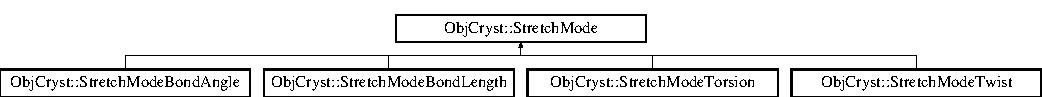
\includegraphics[height=2cm]{a00103}
\end{center}
\end{figure}
\subsubsection*{Public Member Functions}
\begin{DoxyCompactItemize}
\item 
{\bfseries TextureMarchDollase} (const {\bf ScatteringData} \&data)\label{a00103_a68c09384efe47c70c8f43fb877dfc571}

\item 
virtual const string \& {\bf GetName} () const \label{a00103_a8be04714cbb7f98307fa90b044360e35}

\begin{DoxyCompactList}\small\item\em Get the name of this object. \item\end{DoxyCompactList}\item 
virtual const string \& {\bf GetClassName} () const \label{a00103_a2b1002c1ed071f53b2a6f1b953527cc2}

\begin{DoxyCompactList}\small\item\em Get the name of the class. \item\end{DoxyCompactList}\item 
void {\bfseries AddPhase} (const REAL fraction, const REAL coeffMarch, const REAL h, const REAL k, const REAL l)\label{a00103_a88fe286c7547b841edecc905b1a95b84}

\item 
void {\bfseries SetPhasePar} (const unsigned int i, const REAL fraction, const REAL coeffMarch, const REAL h, const REAL k, const REAL l)\label{a00103_ae5cb3330830822cb4ce7d23083296c53}

\item 
void {\bfseries DeletePhase} (const unsigned int i)\label{a00103_a7290f7949ee2c4e302017f24d3994da1}

\item 
unsigned int {\bfseries GetNbPhase} () const \label{a00103_ae3f55de726d50dbf86d7daa4c629a7df}

\item 
REAL {\bfseries GetFraction} (const unsigned int i) const \label{a00103_a02e5f7f948832765eba593759c62dcb4}

\item 
REAL {\bfseries GetMarchCoeff} (const unsigned int i) const \label{a00103_ae2f4479ae167d57ab66d952bb9fa8702}

\item 
REAL {\bfseries GetPhaseH} (const unsigned int i) const \label{a00103_af93dff2dfc82d85dd1d6b6e343fc20e0}

\item 
REAL {\bfseries GetPhaseK} (const unsigned int i) const \label{a00103_a33eba37e0060eb34ea56fe997886966f}

\item 
REAL {\bfseries GetPhaseL} (const unsigned int i) const \label{a00103_a39111e8d14fe437bc5638909fe9b50bf}

\item 
virtual void {\bf GlobalOptRandomMove} (const REAL mutationAmplitude, const {\bf RefParType} $\ast$type={\bf gpRefParTypeObjCryst})
\begin{DoxyCompactList}\small\item\em Make a random move of the current configuration. \item\end{DoxyCompactList}\item 
virtual REAL {\bfseries GetBiasingCost} () const \label{a00103_a37b873011cdb7443876f2954a00d1fe1}

\item 
virtual void {\bf XMLOutput} (ostream \&os, int indent=0) const 
\begin{DoxyCompactList}\small\item\em Output to stream in well-\/formed XML. \item\end{DoxyCompactList}\item 
virtual void {\bf XMLInput} (istream \&is, const {\bf XMLCrystTag} \&tag)
\begin{DoxyCompactList}\small\item\em Input From stream. \item\end{DoxyCompactList}\item 
virtual void {\bf BeginOptimization} (const bool allowApproximations=false, const bool enableRestraints=false)
\begin{DoxyCompactList}\small\item\em This should be called by any optimization class at the begining of an optimization. \item\end{DoxyCompactList}\item 
virtual void {\bf TagNewBestConfig} () const 
\begin{DoxyCompactList}\small\item\em During a global optimization, tells the object that the current config is the latest \char`\"{}best\char`\"{} config. \item\end{DoxyCompactList}\end{DoxyCompactItemize}
\subsubsection*{Protected Member Functions}
\begin{DoxyCompactItemize}
\item 
virtual void {\bf CalcCorr} () const \label{a00103_a1c2c3c1fe88571b2a5b771ab86128240}

\begin{DoxyCompactList}\small\item\em Do the computation of corrected intensities. \item\end{DoxyCompactList}\item 
void {\bfseries DeleteAllPhase} ()\label{a00103_a2c81cc2848f052c2900d135631a7e5ba}

\end{DoxyCompactItemize}
\subsubsection*{Protected Attributes}
\begin{DoxyCompactItemize}
\item 
{\bf ObjRegistry}$<$ {\bf TexturePhaseMarchDollase} $>$ {\bfseries mPhaseRegistry}\label{a00103_a5036a20bd0edc8c003c317ca3d11bd85}

\item 
{\bf RefinableObjClock} {\bfseries mClockTexturePar}\label{a00103_aa2c0a0db3b5c9178d1d61125ac72349e}

\item 
unsigned long {\bf mNbReflUsed}
\begin{DoxyCompactList}\small\item\em Number of reflexion for which the calculation is actually done. \item\end{DoxyCompactList}\end{DoxyCompactItemize}


\subsubsection{Detailed Description}
Texture correction using the March-\/Dollase model. This can include several phases. 

\subsubsection{Member Function Documentation}
\index{ObjCryst::TextureMarchDollase@{ObjCryst::TextureMarchDollase}!BeginOptimization@{BeginOptimization}}
\index{BeginOptimization@{BeginOptimization}!ObjCryst::TextureMarchDollase@{ObjCryst::TextureMarchDollase}}
\paragraph[{BeginOptimization}]{\setlength{\rightskip}{0pt plus 5cm}virtual void ObjCryst::TextureMarchDollase::BeginOptimization (const bool {\em allowApproximations} = {\ttfamily false}, \/  const bool {\em enableRestraints} = {\ttfamily false})\hspace{0.3cm}{\ttfamily  [virtual]}}\hfill\label{a00103_a73f6148d035bbdeb98b0115d76fe48a8}


This should be called by any optimization class at the begining of an optimization. This will also check that everything is ready, eg call the \doxyref{RefinableObj::Prepare()}{p.}{a00070_a48d11671e7f8699f7bc24077585c5e0f} function. This also affects all sub-\/objects. \begin{DoxyNote}{Note}
this may be called several time for some objects which are used by several other objects, or for nested optimizations (e.g. least-\/squares optimizations inside a global one).

\doxyref{EndOptimization()}{p.}{a00070_ab0035f6164cb24ace67b51b11993a851} must be called at the end of the optimization, the same number of time \doxyref{BeginOptimization()}{p.}{a00103_a73f6148d035bbdeb98b0115d76fe48a8} was called !
\end{DoxyNote}

\begin{DoxyParams}{Parameters}
\item[{\em allowApproximations,:}]if true, then the object can use faster but less precise functions during the optimization. This is useful for global optimization not using derivatives. \item[{\em enableRestraints,:}]\end{DoxyParams}
\begin{Desc}
\item[{\bf Deprecated}]if true, then restrained parameters will be allowed to go beyond theur hard limits. This implies that the algorithm will take into account the cost (penalty) related to the restraints. Objects which do not use restraints will simply ignore this. WARNING: this parameter may be removed with the new likelihood scheme. \end{Desc}


Reimplemented from {\bf ObjCryst::RefinableObj} \doxyref{}{p.}{a00070_ababd8f2916e41a20d2c1b21f6ffefe96}.\index{ObjCryst::TextureMarchDollase@{ObjCryst::TextureMarchDollase}!GlobalOptRandomMove@{GlobalOptRandomMove}}
\index{GlobalOptRandomMove@{GlobalOptRandomMove}!ObjCryst::TextureMarchDollase@{ObjCryst::TextureMarchDollase}}
\paragraph[{GlobalOptRandomMove}]{\setlength{\rightskip}{0pt plus 5cm}virtual void ObjCryst::TextureMarchDollase::GlobalOptRandomMove (const REAL {\em mutationAmplitude}, \/  const {\bf RefParType} $\ast$ {\em type} = {\ttfamily {\bf gpRefParTypeObjCryst}})\hspace{0.3cm}{\ttfamily  [virtual]}}\hfill\label{a00103_a43d8d96c3f14d9d01145dfbefb759e6a}


Make a random move of the current configuration. This is for global optimization algorithms. the moves for each parameter are less than their global optimization step, multiplied by the mutation amplitude.

\begin{DoxyWarning}{Warning}
: this makes a random move for the parameter declared for this object, and it is the duty of the object to decide whether the included objects should be moved and how. (eg an algorithm should only call for a move with the top object, and this object decides how he and his sub-\/objects moves). By default (\doxyref{RefinableObj}{p.}{a00070} implementation) all included objects are moved recursively.
\end{DoxyWarning}
\doxyref{RefinableObj}{p.}{a00070}:: 
\begin{DoxyParams}{Parameters}
\item[{\em mutationAmplitude,:}]multiplier for the maximum move amplitude, for all parameters \item[{\em type,:}]restrain the change exclusively to parameters of a given type (same type or descendant from this \doxyref{RefParType}{p.}{a00079}). \end{DoxyParams}


Reimplemented from {\bf ObjCryst::RefinableObj} \doxyref{}{p.}{a00070_a18375c8525ae38c481ba77e9cf9d67c1}.\index{ObjCryst::TextureMarchDollase@{ObjCryst::TextureMarchDollase}!TagNewBestConfig@{TagNewBestConfig}}
\index{TagNewBestConfig@{TagNewBestConfig}!ObjCryst::TextureMarchDollase@{ObjCryst::TextureMarchDollase}}
\paragraph[{TagNewBestConfig}]{\setlength{\rightskip}{0pt plus 5cm}virtual void ObjCryst::TextureMarchDollase::TagNewBestConfig () const\hspace{0.3cm}{\ttfamily  [virtual]}}\hfill\label{a00103_a972d51af36bfd317f794c87841c58b5a}


During a global optimization, tells the object that the current config is the latest \char`\"{}best\char`\"{} config. This can be used by the object to make more intellingent random moves (use with caution: highly experimental !). 

Reimplemented from {\bf ObjCryst::RefinableObj} \doxyref{}{p.}{a00070_a3cb4cc924d39576618184eccd4321cf6}.\index{ObjCryst::TextureMarchDollase@{ObjCryst::TextureMarchDollase}!XMLInput@{XMLInput}}
\index{XMLInput@{XMLInput}!ObjCryst::TextureMarchDollase@{ObjCryst::TextureMarchDollase}}
\paragraph[{XMLInput}]{\setlength{\rightskip}{0pt plus 5cm}virtual void ObjCryst::TextureMarchDollase::XMLInput (istream \& {\em is}, \/  const {\bf XMLCrystTag} \& {\em tag})\hspace{0.3cm}{\ttfamily  [virtual]}}\hfill\label{a00103_a26ae81ce2e09c173d200c9a61cb67161}


Input From stream. \begin{Desc}
\item[{\bf Todo}]Add an bool XMLInputTag(is,tag) function to recognize all the tags from the stream. So that each inherited class can use the XMLInputTag function from its parent (ie take advantage of inheritance). The children class would first try to interpret the tag, then if unsuccessful would pass it to its parent (thus allowing overloading), etc... \end{Desc}


Reimplemented from {\bf ObjCryst::RefinableObj} \doxyref{}{p.}{a00070_ac13a4045c3f187879443c8615c38d623}.\index{ObjCryst::TextureMarchDollase@{ObjCryst::TextureMarchDollase}!XMLOutput@{XMLOutput}}
\index{XMLOutput@{XMLOutput}!ObjCryst::TextureMarchDollase@{ObjCryst::TextureMarchDollase}}
\paragraph[{XMLOutput}]{\setlength{\rightskip}{0pt plus 5cm}virtual void ObjCryst::TextureMarchDollase::XMLOutput (ostream \& {\em os}, \/  int {\em indent} = {\ttfamily 0}) const\hspace{0.3cm}{\ttfamily  [virtual]}}\hfill\label{a00103_a09d994c3344a276ba65563fb9f1b45ca}


Output to stream in well-\/formed XML. \begin{Desc}
\item[{\bf Todo}]Use inheritance.. as for XMLInputTag()... \end{Desc}


Reimplemented from {\bf ObjCryst::RefinableObj} \doxyref{}{p.}{a00070_a7b9b6ed0f8dcf753d398c35e073de973}.

\subsubsection{Member Data Documentation}
\index{ObjCryst::TextureMarchDollase@{ObjCryst::TextureMarchDollase}!mNbReflUsed@{mNbReflUsed}}
\index{mNbReflUsed@{mNbReflUsed}!ObjCryst::TextureMarchDollase@{ObjCryst::TextureMarchDollase}}
\paragraph[{mNbReflUsed}]{\setlength{\rightskip}{0pt plus 5cm}unsigned long {\bf ObjCryst::TextureMarchDollase::mNbReflUsed}\hspace{0.3cm}{\ttfamily  [mutable, protected]}}\hfill\label{a00103_a243ea853b7d3179f9474386ed296783c}


Number of reflexion for which the calculation is actually done. This is automaticaly updated during CalcCorr, from the parent \doxyref{ScatteringData::GetMaxSinThetaOvLambda()}{p.}{a00088_ad682b6879c751fd4d241a198b1893e6e} 

The documentation for this class was generated from the following file:\begin{DoxyCompactItemize}
\item 
ScatteringCorr.h\end{DoxyCompactItemize}

\subsection{Obj\-Cryst\-:\-:Stretch\-Mode Struct Reference}
\label{a00104}\index{Obj\-Cryst\-::\-Stretch\-Mode@{Obj\-Cryst\-::\-Stretch\-Mode}}


Abstract base Stretch Mode for \doxyref{Molecule}{p.}{a00054} objects.  


Inheritance diagram for Obj\-Cryst\-:\-:Stretch\-Mode\-:\begin{figure}[H]
\begin{center}
\leavevmode
\includegraphics[height=1.302326cm]{a00104}
\end{center}
\end{figure}
\subsubsection*{Public Member Functions}
\begin{DoxyCompactItemize}
\item 
virtual void {\bf Calc\-Deriv} (const bool derivllk=true) const =0
\begin{DoxyCompactList}\small\item\em Calculate the derivative of the \doxyref{Molecule}{p.}{a00054}'s Log(likelihood) and atomic positions versus a change of the bond length. \end{DoxyCompactList}\item 
virtual void {\bf Print} (ostream \&os, bool full=true) const =0\label{a00104_a78c180042fce5981fe0e97071d986362}

\begin{DoxyCompactList}\small\item\em Print one-\/line list of atoms moved. \end{DoxyCompactList}\item 
virtual void {\bf Stretch} (const R\-E\-A\-L change)=0\label{a00104_a1f3e7e8fc43baed619b61203ea77c143}

\begin{DoxyCompactList}\small\item\em Move the atoms according to this mode. \end{DoxyCompactList}\item 
virtual void {\bf Random\-Stretch} (const R\-E\-A\-L amplitude)=0\label{a00104_a459057c6cd3d2cb1010676b54ebfe988}

\begin{DoxyCompactList}\small\item\em Move the atoms according to this mode, randomly. \end{DoxyCompactList}\end{DoxyCompactItemize}
\subsubsection*{Public Attributes}
\begin{DoxyCompactItemize}
\item 
std\-::map$<$ const {\bf Mol\-Bond} $\ast$, R\-E\-A\-L $>$ {\bf mvp\-Broken\-Bond}\label{a00104_a6628812c69f20a7a18a7a3759b5c961c}

\begin{DoxyCompactList}\small\item\em List of bond restraints affected by this mode The key is the restraint, the value is the derivative of the L\-L\-K associated. \end{DoxyCompactList}\item 
std\-::map$<$ const {\bf Mol\-Bond\-Angle} \\*
$\ast$, R\-E\-A\-L $>$ {\bf mvp\-Broken\-Bond\-Angle}\label{a00104_a2a46f6bd997850be6736e4b5746deeed}

\begin{DoxyCompactList}\small\item\em List of bond angle restraints modified by this mode The key is the restraint, the value is the derivative of the L\-L\-K associated. \end{DoxyCompactList}\item 
std\-::map$<$ const \\*
{\bf Mol\-Dihedral\-Angle} $\ast$, R\-E\-A\-L $>$ {\bf mvp\-Broken\-Dihedral\-Angle}\label{a00104_a84257bc829a3d612b68046d33685e59e}

\begin{DoxyCompactList}\small\item\em List of dihedral angle restraints modified by this mode The key is the restraint, the value is the derivative of the L\-L\-K associated. \end{DoxyCompactList}\item 
R\-E\-A\-L {\bf m\-L\-L\-K\-Deriv}\label{a00104_ac6614921c015de3f6d67b22ae512a66c}

\begin{DoxyCompactList}\small\item\em Derivative of the \doxyref{Molecule}{p.}{a00054}'s Log(likelihood) versus a change of the bond length. \end{DoxyCompactList}\item 
std\-::map$<$ const {\bf Mol\-Atom} $\ast$, {\bf X\-Y\-Z} $>$ {\bf m\-Deriv\-X\-Y\-Z}\label{a00104_a4a25093e177c56be142acc954149c110}

\begin{DoxyCompactList}\small\item\em Derivative of the atomic positions versus a change of the bond length. \end{DoxyCompactList}\item 
{\bf Molecule} $\ast$ {\bf mp\-Mol}\label{a00104_a380bd0aef1e5be1f681364e0f754f3e3}

\begin{DoxyCompactList}\small\item\em The \doxyref{Molecule}{p.}{a00054} corresponding to this stretch mode. \end{DoxyCompactList}\item 
R\-E\-A\-L {\bf m\-Base\-Amplitude}
\begin{DoxyCompactList}\small\item\em The recommended change amplitude, for a base global optimization displacement, to obtain an average 0.\-1 Angstroem displacement. \end{DoxyCompactList}\end{DoxyCompactItemize}


\subsubsection{Detailed Description}
Abstract base Stretch Mode for \doxyref{Molecule}{p.}{a00054} objects. 



\subsubsection{Member Function Documentation}
\index{Obj\-Cryst\-::\-Stretch\-Mode@{Obj\-Cryst\-::\-Stretch\-Mode}!Calc\-Deriv@{Calc\-Deriv}}
\index{Calc\-Deriv@{Calc\-Deriv}!ObjCryst::StretchMode@{Obj\-Cryst\-::\-Stretch\-Mode}}
\paragraph[{Calc\-Deriv}]{\setlength{\rightskip}{0pt plus 5cm}virtual void Obj\-Cryst\-::\-Stretch\-Mode\-::\-Calc\-Deriv (
\begin{DoxyParamCaption}
\item[{const bool}]{derivllk = {\ttfamily true}}
\end{DoxyParamCaption}
) const\hspace{0.3cm}{\ttfamily [pure virtual]}}\label{a00104_a5b5ab5f9819c047a49719a330722d419}


Calculate the derivative of the \doxyref{Molecule}{p.}{a00054}'s Log(likelihood) and atomic positions versus a change of the bond length. 

The result is stored in m\-L\-L\-K\-Deriv and m\-L\-L\-K\-Deriv\-X\-Y\-Z, as well as in the various lists of restraints broken by this mode.


\begin{DoxyParams}{Parameters}
{\em derivllk,\-:} & if false, the derivative of the overall llk will not be computed, only the derivative of the atomic positions. \\
\hline
\end{DoxyParams}


Implemented in {\bf Obj\-Cryst\-::\-Stretch\-Mode\-Twist} \doxyref{}{p.}{a00109_afd1ac754d10507e1c9bed829a4eaeb79}, {\bf Obj\-Cryst\-::\-Stretch\-Mode\-Torsion} \doxyref{}{p.}{a00108_abecf1074b05ba13fd938667399df110e}, {\bf Obj\-Cryst\-::\-Stretch\-Mode\-Bond\-Angle} \doxyref{}{p.}{a00105_acdc082c4cb5b4f38fed6049bf7b1eb9c}, and {\bf Obj\-Cryst\-::\-Stretch\-Mode\-Bond\-Length} \doxyref{}{p.}{a00106_a72bab02ebf84cbf65cf2703e74c1e02e}.



\subsubsection{Member Data Documentation}
\index{Obj\-Cryst\-::\-Stretch\-Mode@{Obj\-Cryst\-::\-Stretch\-Mode}!m\-Base\-Amplitude@{m\-Base\-Amplitude}}
\index{m\-Base\-Amplitude@{m\-Base\-Amplitude}!ObjCryst::StretchMode@{Obj\-Cryst\-::\-Stretch\-Mode}}
\paragraph[{m\-Base\-Amplitude}]{\setlength{\rightskip}{0pt plus 5cm}R\-E\-A\-L Obj\-Cryst\-::\-Stretch\-Mode\-::m\-Base\-Amplitude}\label{a00104_aa8dc03e2bd6840d13964dd6751c39fae}


The recommended change amplitude, for a base global optimization displacement, to obtain an average 0.\-1 Angstroem displacement. 

This is learnt at the beginning of an optimization.

This can be superseeded to respect any restraint. 

The documentation for this struct was generated from the following file\-:\begin{DoxyCompactItemize}
\item 
Molecule.\-h\end{DoxyCompactItemize}

\subsection{Obj\-Cryst\-:\-:Stretch\-Mode\-Bond\-Angle Struct Reference}
\label{a00105}\index{Obj\-Cryst\-::\-Stretch\-Mode\-Bond\-Angle@{Obj\-Cryst\-::\-Stretch\-Mode\-Bond\-Angle}}


Atoms moved when changing a bond angle.  


Inheritance diagram for Obj\-Cryst\-:\-:Stretch\-Mode\-Bond\-Angle\-:\begin{figure}[H]
\begin{center}
\leavevmode
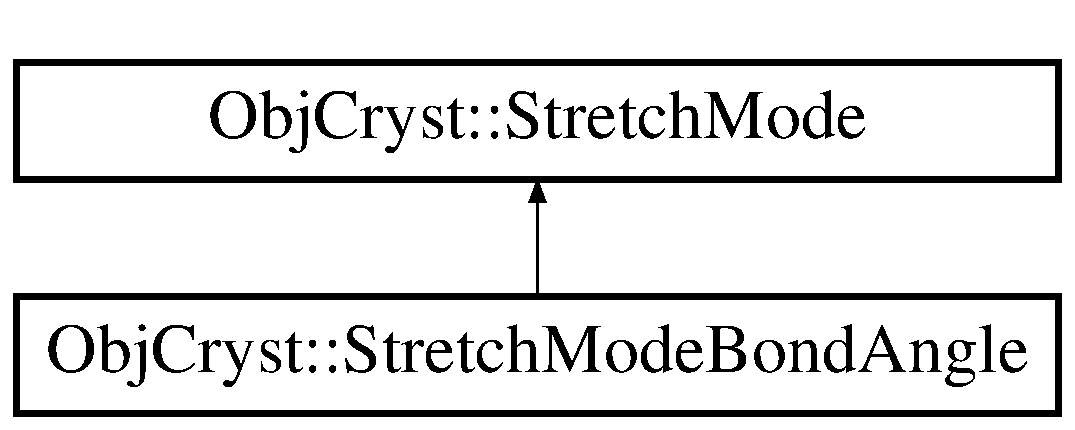
\includegraphics[height=2.000000cm]{a00105}
\end{center}
\end{figure}
\subsubsection*{Public Member Functions}
\begin{DoxyCompactItemize}
\item 
{\bf Stretch\-Mode\-Bond\-Angle} ({\bf Mol\-Atom} \&at0, {\bf Mol\-Atom} \&at1, {\bf Mol\-Atom} \&at2, const {\bf Mol\-Bond\-Angle} $\ast$p\-Bond\-Angle)\label{a00105_aa1fbf3238722b663b083c999cf1b5c57}

\begin{DoxyCompactList}\small\item\em Constructor If p\-Bond\-Angle!=0, the bond angle length restraint is respected. \end{DoxyCompactList}\item 
virtual void {\bf Calc\-Deriv} (const bool derivllk=true) const 
\begin{DoxyCompactList}\small\item\em Calculate the derivative of the \doxyref{Molecule}{p.}{a00054}'s Log(likelihood) and atomic positions versus a change of the bond length. \end{DoxyCompactList}\item 
virtual void {\bf Print} (ostream \&os, bool full=true) const \label{a00105_a77e72910a64e3351a05a2f7ac47033c0}

\begin{DoxyCompactList}\small\item\em Print one-\/line list of atoms moved. \end{DoxyCompactList}\item 
virtual void {\bf Stretch} (const R\-E\-A\-L change)\label{a00105_aff6934e2b0a048d164228348f87f544d}

\begin{DoxyCompactList}\small\item\em Move the atoms according to this mode. \end{DoxyCompactList}\item 
virtual void {\bf Random\-Stretch} (const R\-E\-A\-L amplitude)\label{a00105_a7e3006f5ecd0d683ec669475c5f21394}

\begin{DoxyCompactList}\small\item\em Move the atoms according to this mode, randomly. \end{DoxyCompactList}\end{DoxyCompactItemize}
\subsubsection*{Public Attributes}
\begin{DoxyCompactItemize}
\item 
{\bf Mol\-Atom} $\ast$ {\bf mp\-Atom0}\label{a00105_a63bc5bb54f0d298fb47b7bf86e8c2ff5}

\begin{DoxyCompactList}\small\item\em The first atom. \end{DoxyCompactList}\item 
{\bf Mol\-Atom} $\ast$ {\bf mp\-Atom1}\label{a00105_aa5b52fcece40cd41c93eeb8b1dfec939}

\begin{DoxyCompactList}\small\item\em The second atom. \end{DoxyCompactList}\item 
{\bf Mol\-Atom} $\ast$ {\bf mp\-Atom2}\label{a00105_a08c6b4fde05610d0242bfd7b4a6acc3f}

\begin{DoxyCompactList}\small\item\em The third atom. \end{DoxyCompactList}\item 
const {\bf Mol\-Bond\-Angle} $\ast$ {\bf mp\-Bond\-Angle}\label{a00105_ab173d155feb360d0b95b5cd35f346da5}

\begin{DoxyCompactList}\small\item\em The (optional) bond angle restraint which this stretch mode should respect. \end{DoxyCompactList}\item 
set$<$ {\bf Mol\-Atom} $\ast$ $>$ {\bf mv\-Rotated\-Atom\-List}
\begin{DoxyCompactList}\small\item\em The set of atoms that are to be rotated around the direction going through at1 and perpendicular to the at0-\/at1-\/at2 plane. \end{DoxyCompactList}\end{DoxyCompactItemize}


\subsubsection{Detailed Description}
Atoms moved when changing a bond angle. 

This should be merged (or have an inheritance relation) with \doxyref{Mol\-Bond\-Angle}{p.}{a00052}. 

\subsubsection{Member Function Documentation}
\index{Obj\-Cryst\-::\-Stretch\-Mode\-Bond\-Angle@{Obj\-Cryst\-::\-Stretch\-Mode\-Bond\-Angle}!Calc\-Deriv@{Calc\-Deriv}}
\index{Calc\-Deriv@{Calc\-Deriv}!ObjCryst::StretchModeBondAngle@{Obj\-Cryst\-::\-Stretch\-Mode\-Bond\-Angle}}
\paragraph[{Calc\-Deriv}]{\setlength{\rightskip}{0pt plus 5cm}virtual void Obj\-Cryst\-::\-Stretch\-Mode\-Bond\-Angle\-::\-Calc\-Deriv (
\begin{DoxyParamCaption}
\item[{const bool}]{derivllk = {\ttfamily true}}
\end{DoxyParamCaption}
) const\hspace{0.3cm}{\ttfamily [virtual]}}\label{a00105_acdc082c4cb5b4f38fed6049bf7b1eb9c}


Calculate the derivative of the \doxyref{Molecule}{p.}{a00054}'s Log(likelihood) and atomic positions versus a change of the bond length. 

The result is stored in m\-L\-L\-K\-Deriv and m\-L\-L\-K\-Deriv\-X\-Y\-Z, as well as in the various lists of restraints broken by this mode.


\begin{DoxyParams}{Parameters}
{\em derivllk,\-:} & if false, the derivative of the overall llk will not be computed, only the derivative of the atomic positions. \\
\hline
\end{DoxyParams}


Implements {\bf Obj\-Cryst\-::\-Stretch\-Mode} \doxyref{}{p.}{a00104_a5b5ab5f9819c047a49719a330722d419}.



\subsubsection{Member Data Documentation}
\index{Obj\-Cryst\-::\-Stretch\-Mode\-Bond\-Angle@{Obj\-Cryst\-::\-Stretch\-Mode\-Bond\-Angle}!mv\-Rotated\-Atom\-List@{mv\-Rotated\-Atom\-List}}
\index{mv\-Rotated\-Atom\-List@{mv\-Rotated\-Atom\-List}!ObjCryst::StretchModeBondAngle@{Obj\-Cryst\-::\-Stretch\-Mode\-Bond\-Angle}}
\paragraph[{mv\-Rotated\-Atom\-List}]{\setlength{\rightskip}{0pt plus 5cm}set$<${\bf Mol\-Atom} $\ast$$>$ Obj\-Cryst\-::\-Stretch\-Mode\-Bond\-Angle\-::mv\-Rotated\-Atom\-List}\label{a00105_a1d70964f33ea3a594efd2c3a595816a6}


The set of atoms that are to be rotated around the direction going through at1 and perpendicular to the at0-\/at1-\/at2 plane. 



The documentation for this struct was generated from the following file\-:\begin{DoxyCompactItemize}
\item 
Molecule.\-h\end{DoxyCompactItemize}

\subsection{Obj\+Cryst\+:\+:Molecule\+:\+:Stretch\+Mode\+Group Struct Reference}
\label{a00106}\index{Obj\+Cryst\+::\+Molecule\+::\+Stretch\+Mode\+Group@{Obj\+Cryst\+::\+Molecule\+::\+Stretch\+Mode\+Group}}


Group of concurrent Stretch\+Modes (affecting common restraints) A given stretch mode can only belong to one group.  


\subsubsection*{Public Attributes}
\begin{DoxyCompactItemize}
\item 
std\+::set$<$ {\bf Stretch\+Mode} $\ast$ $>$ {\bfseries mvp\+Stretch\+Mode}\label{a00106_a63c54cd06ab4a7b838cc686214d41750}

\item 
std\+::set$<$ const {\bf Mol\+Bond} $\ast$ $>$ {\bfseries mvp\+Broken\+Bond}\label{a00106_a3f6e58dc0887b43c2187080b27e2836f}

\item 
std\+::set$<$ const {\bf Mol\+Bond\+Angle} $\ast$ $>$ {\bfseries mvp\+Broken\+Bond\+Angle}\label{a00106_a2b325fc86d71b14c62efc683e05b0fe0}

\item 
std\+::set$<$ const \\*
{\bf Mol\+Dihedral\+Angle} $\ast$ $>$ {\bfseries mvp\+Broken\+Dihedral\+Angle}\label{a00106_aaaee134991cbfe70408dc4b310981c63}

\end{DoxyCompactItemize}


\subsubsection{Detailed Description}
Group of concurrent Stretch\+Modes (affecting common restraints) A given stretch mode can only belong to one group. 



The documentation for this struct was generated from the following file\+:\begin{DoxyCompactItemize}
\item 
Molecule.\+h\end{DoxyCompactItemize}

\subsection{\-Obj\-Cryst\-:\-:\-Tracker \-Class \-Reference}
\label{a00107}\index{\-Obj\-Cryst\-::\-Tracker@{\-Obj\-Cryst\-::\-Tracker}}


\-A class to track the variation of parameters as a function of a number of cycles/trials.  


\-Inheritance diagram for \-Obj\-Cryst\-:\-:\-Tracker\-:\begin{figure}[H]
\begin{center}
\leavevmode
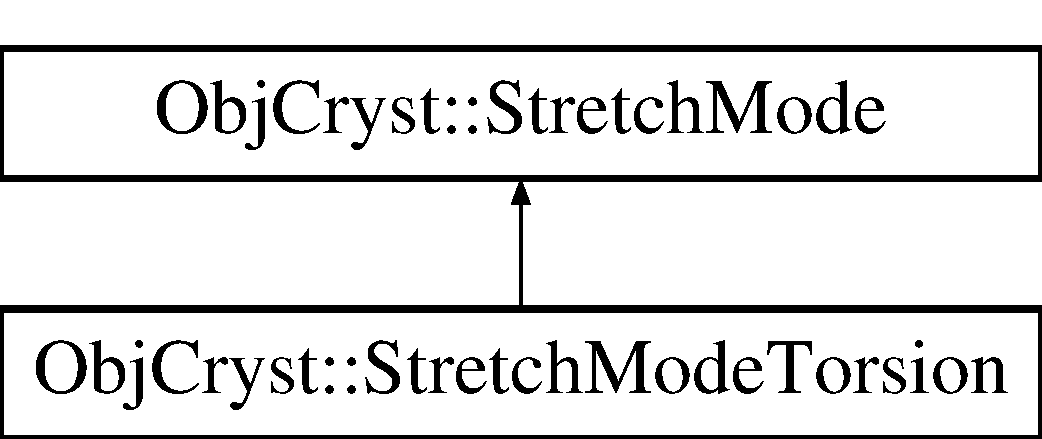
\includegraphics[height=2.000000cm]{a00107}
\end{center}
\end{figure}
\subsubsection*{\-Public \-Member \-Functions}
\begin{DoxyCompactItemize}
\item 
{\bfseries \-Tracker} (const std\-::string \&name)\label{a00107_a57d89249ba910902e6ef6a33dcd3ee8c}

\item 
const std\-::string \& {\bfseries \-Get\-Name} () const \label{a00107_ad93197775f7d0a3b52eb199a9ed1c958}

\item 
void {\bfseries \-Append\-Value} (const long trial)\label{a00107_ae50d08700a131d280f8a19a58274bfe7}

\item 
void {\bf \-Clear} ()\label{a00107_abdac1cff42cfd8d66e10977a5a9066b3}

\begin{DoxyCompactList}\small\item\em \-Removes all stored values. \end{DoxyCompactList}\item 
const std\-::map$<$ long, \-R\-E\-A\-L $>$ \& {\bfseries \-Get\-Values} () const \label{a00107_a882fe8d7c193662613d4a9ab262a2417}

\item 
std\-::map$<$ long, \-R\-E\-A\-L $>$ \& {\bfseries \-Get\-Values} ()\label{a00107_a4f889b0d29a403c597040c5b88f4ffa8}

\end{DoxyCompactItemize}
\subsubsection*{\-Protected \-Member \-Functions}
\begin{DoxyCompactItemize}
\item 
virtual \-R\-E\-A\-L {\bfseries \-Read\-Value} ()=0\label{a00107_a14096d99b76d3ffac16553f6434f97ce}

\end{DoxyCompactItemize}
\subsubsection*{\-Protected \-Attributes}
\begin{DoxyCompactItemize}
\item 
std\-::map$<$ long, \-R\-E\-A\-L $>$ {\bfseries mv\-Values}\label{a00107_adcd7db9240b7c6432a1fe2f0daec2d24}

\item 
std\-::string {\bfseries m\-Name}\label{a00107_a64fee6086f7c35c89c72d703903a1b26}

\end{DoxyCompactItemize}


\subsubsection{\-Detailed \-Description}
\-A class to track the variation of parameters as a function of a number of cycles/trials. 

\-This is an abstract base class. 

\-The documentation for this class was generated from the following file\-:\begin{DoxyCompactItemize}
\item 
\-Tracker.\-h\end{DoxyCompactItemize}

\subsection{Obj\-Cryst\-:\-:Stretch\-Mode\-Twist Struct Reference}
\label{a00108}\index{Obj\-Cryst\-::\-Stretch\-Mode\-Twist@{Obj\-Cryst\-::\-Stretch\-Mode\-Twist}}


Atoms moved {\itshape between} two other atoms, using a \char`\"{}twist\char`\"{} of their positions -\/ only small twists of their positions are allowed to avoid breaking restraints too much.  


Inheritance diagram for Obj\-Cryst\-:\-:Stretch\-Mode\-Twist\-:\begin{figure}[H]
\begin{center}
\leavevmode
\includegraphics[height=2.000000cm]{a00108}
\end{center}
\end{figure}
\subsubsection*{Public Member Functions}
\begin{DoxyCompactItemize}
\item 
{\bf Stretch\-Mode\-Twist} ({\bf Mol\-Atom} \&at1, {\bf Mol\-Atom} \&at2)\label{a00108_a6ed224b06c93f630ccb7bf7920f054a9}

\begin{DoxyCompactList}\small\item\em Constructor If p\-Dihedral\-Angle!=0, the dihedral angle length restraint is respected. \end{DoxyCompactList}\item 
virtual void {\bf Calc\-Deriv} (const bool derivllk=true) const 
\begin{DoxyCompactList}\small\item\em Calculate the derivative of the \doxyref{Molecule}{p.}{a00053}'s Log(likelihood) and atomic positions versus a change of the bond length. \end{DoxyCompactList}\item 
virtual void {\bf Print} (ostream \&os, bool full=true) const \label{a00108_a6bd2ea406272adfbaa047e49079893b7}

\begin{DoxyCompactList}\small\item\em Print one-\/line list of atoms moved. \end{DoxyCompactList}\item 
virtual void {\bf Stretch} (const R\-E\-A\-L change)\label{a00108_a9eb2c84a7567bd022677f5ded0d18a84}

\begin{DoxyCompactList}\small\item\em Move the atoms according to this mode. \end{DoxyCompactList}\item 
virtual void {\bf Random\-Stretch} (const R\-E\-A\-L amplitude)\label{a00108_af38a4c05e360733d48039c3becbcb3bd}

\begin{DoxyCompactList}\small\item\em Move the atoms according to this mode, randomly. \end{DoxyCompactList}\end{DoxyCompactItemize}
\subsubsection*{Public Attributes}
\begin{DoxyCompactItemize}
\item 
{\bf Mol\-Atom} $\ast$ {\bf mp\-Atom1}\label{a00108_ad744e9f68b07367752ed7c03d381a30c}

\begin{DoxyCompactList}\small\item\em The first atom. \end{DoxyCompactList}\item 
{\bf Mol\-Atom} $\ast$ {\bf mp\-Atom2}\label{a00108_a36180a825c130a18a59c6cfe1a44398c}

\begin{DoxyCompactList}\small\item\em The second atom. \end{DoxyCompactList}\item 
set$<$ {\bf Mol\-Atom} $\ast$ $>$ {\bf mv\-Rotated\-Atom\-List}\label{a00108_a5b3c7f8a0bf81c04ca39fcc88e596f22}

\begin{DoxyCompactList}\small\item\em The set of atoms that are to be rotated around at1-\/at2. \end{DoxyCompactList}\end{DoxyCompactItemize}


\subsubsection{Detailed Description}
Atoms moved {\itshape between} two other atoms, using a \char`\"{}twist\char`\"{} of their positions -\/ only small twists of their positions are allowed to avoid breaking restraints too much. 

Also, the atoms in the middle between the two reference atoms are more displaced than the one closer, to help avoid breaking restraints. 

\subsubsection{Member Function Documentation}
\index{Obj\-Cryst\-::\-Stretch\-Mode\-Twist@{Obj\-Cryst\-::\-Stretch\-Mode\-Twist}!Calc\-Deriv@{Calc\-Deriv}}
\index{Calc\-Deriv@{Calc\-Deriv}!ObjCryst::StretchModeTwist@{Obj\-Cryst\-::\-Stretch\-Mode\-Twist}}
\paragraph[{Calc\-Deriv}]{\setlength{\rightskip}{0pt plus 5cm}virtual void Obj\-Cryst\-::\-Stretch\-Mode\-Twist\-::\-Calc\-Deriv (
\begin{DoxyParamCaption}
\item[{const bool}]{derivllk = {\ttfamily true}}
\end{DoxyParamCaption}
) const\hspace{0.3cm}{\ttfamily [virtual]}}\label{a00108_afd1ac754d10507e1c9bed829a4eaeb79}


Calculate the derivative of the \doxyref{Molecule}{p.}{a00053}'s Log(likelihood) and atomic positions versus a change of the bond length. 

The result is stored in m\-L\-L\-K\-Deriv and m\-L\-L\-K\-Deriv\-X\-Y\-Z, as well as in the various lists of restraints broken by this mode.


\begin{DoxyParams}{Parameters}
{\em derivllk} & if false, the derivative of the overall llk will not be computed, only the derivative of the atomic positions. \\
\hline
\end{DoxyParams}


Implements {\bf Obj\-Cryst\-::\-Stretch\-Mode} \doxyref{}{p.}{a00103_a5b5ab5f9819c047a49719a330722d419}.



The documentation for this struct was generated from the following file\-:\begin{DoxyCompactItemize}
\item 
Molecule.\-h\end{DoxyCompactItemize}

\subsection{Obj\-Cryst\-:\-:Symmetric\-Pair\-Compare$<$ T $>$ Class Template Reference}
\label{a00109}\index{Obj\-Cryst\-::\-Symmetric\-Pair\-Compare$<$ T $>$@{Obj\-Cryst\-::\-Symmetric\-Pair\-Compare$<$ T $>$}}


Class to compare pairs of objects, with the two objects playing a symmetric role.  


\subsubsection*{Public Member Functions}
\begin{DoxyCompactItemize}
\item 
bool {\bfseries operator()} (const pair$<$ T, T $>$ \&p1, const pair$<$ T, T $>$ \&p2) const \label{a00109_a210b2707d39d9354dba198a0a288c3ab}

\end{DoxyCompactItemize}


\subsubsection{Detailed Description}
\subsubsection*{template$<$class T$>$class Obj\-Cryst\-::\-Symmetric\-Pair\-Compare$<$ T $>$}

Class to compare pairs of objects, with the two objects playing a symmetric role. 

The documentation for this class was generated from the following file\-:\begin{DoxyCompactItemize}
\item 
General.\-h\end{DoxyCompactItemize}

\subsection{Obj\-Cryst\-:\-:Symmetric\-Pair\-Compare$<$ T $>$ Class Template Reference}
\label{a00110}\index{Obj\-Cryst\-::\-Symmetric\-Pair\-Compare$<$ T $>$@{Obj\-Cryst\-::\-Symmetric\-Pair\-Compare$<$ T $>$}}


Class to compare pairs of objects, with the two objects playing a symmetric role.  


\subsubsection*{Public Member Functions}
\begin{DoxyCompactItemize}
\item 
bool {\bfseries operator()} (const pair$<$ T, T $>$ \&p1, const pair$<$ T, T $>$ \&p2) const \label{a00110_a210b2707d39d9354dba198a0a288c3ab}

\end{DoxyCompactItemize}


\subsubsection{Detailed Description}
\subsubsection*{template$<$class T$>$class Obj\-Cryst\-::\-Symmetric\-Pair\-Compare$<$ T $>$}

Class to compare pairs of objects, with the two objects playing a symmetric role. 

The documentation for this class was generated from the following file\-:\begin{DoxyCompactItemize}
\item 
General.\-h\end{DoxyCompactItemize}

\subsection{Obj\+Cryst\+:\+:Texture\+Phase\+March\+Dollase Struct Reference}
\label{a00111}\index{Obj\+Cryst\+::\+Texture\+Phase\+March\+Dollase@{Obj\+Cryst\+::\+Texture\+Phase\+March\+Dollase}}


One texture phase for the March-\/\+Dollase model.  


\subsubsection*{Public Member Functions}
\begin{DoxyCompactItemize}
\item 
{\bfseries Texture\+Phase\+March\+Dollase} (const R\+E\+A\+L f, const R\+E\+A\+L c, const R\+E\+A\+L h, const R\+E\+A\+L k, const R\+E\+A\+L l, {\bf Texture\+March\+Dollase} \&)\label{a00111_a7a17886446b42d17ba97c5f9752fd3f4}

\item 
const string \& {\bfseries Get\+Class\+Name} () const \label{a00111_a79ab7a2e0e08bfa79e056ad5e790bf80}

\item 
const string \& {\bfseries Get\+Name} () const \label{a00111_abc2b62f55a51617adef8bc3cc40e9e34}

\item 
void {\bfseries Set\+Par} (const R\+E\+A\+L f, const R\+E\+A\+L c, const R\+E\+A\+L h, const R\+E\+A\+L k, const R\+E\+A\+L l)\label{a00111_aab4457580c005e68901acb9ce34d5090}

\item 
void {\bfseries X\+M\+L\+Output} (ostream \&os, int indent=0) const \label{a00111_a126f46830b9bfcf6932526f5909e8655}

\item 
void {\bfseries X\+M\+L\+Input} (istream \&is, const {\bf X\+M\+L\+Cryst\+Tag} \&tag)\label{a00111_a8163897408ab5d08ccaf5ddb9ffd4254}

\end{DoxyCompactItemize}
\subsubsection*{Public Attributes}
\begin{DoxyCompactItemize}
\item 
R\+E\+A\+L {\bfseries m\+Fraction}\label{a00111_a9059c8d95baeb8bba194188167fd6ba3}

\item 
R\+E\+A\+L {\bfseries m\+March\+Coeff}\label{a00111_af54a682c4bea01ad89bf09c234e25f92}

\item 
R\+E\+A\+L {\bfseries m\+H}\label{a00111_ad22aba0c945d8bbcb3238f1059410b5a}

\item 
R\+E\+A\+L {\bfseries m\+K}\label{a00111_ad06c88aedc5968653bc895601c6d5754}

\item 
R\+E\+A\+L {\bfseries m\+L}\label{a00111_ae20d183c75da02534d4ef887166ed99d}

\item 
R\+E\+A\+L {\bf m\+Norm}\label{a00111_a3affb0c886c88243f76a7d38f30e10f3}

\begin{DoxyCompactList}\small\item\em Norm of the (H\+K\+L) vector, to keep it constant during optimization. \end{DoxyCompactList}\item 
{\bf Texture\+March\+Dollase} $\ast$ {\bf mp\+Texture\+March\+Dollase}\label{a00111_acf640da43b88a1955cd490fb64f1d1c6}

\begin{DoxyCompactList}\small\item\em The parent \doxyref{Texture\+March\+Dollase}{p.}{a00110} object. \end{DoxyCompactList}\item 
R\+E\+A\+L {\bf m\+Bias\+Fraction}
\begin{DoxyCompactList}\small\item\em Values of parameters towards which the optimization is biased (if biasing is used). \end{DoxyCompactList}\item 
R\+E\+A\+L {\bfseries m\+Bias\+March\+Coeff}\label{a00111_a0dd475c57d0188d354bc25c5778b0172}

\item 
R\+E\+A\+L {\bfseries m\+Bias\+H}\label{a00111_adc4211e8726249e9a4ea1fecbdd3d00d}

\item 
R\+E\+A\+L {\bfseries m\+Bias\+K}\label{a00111_a55bf867c3441f8732c8d39f7f3c506cd}

\item 
R\+E\+A\+L {\bfseries m\+Bias\+L}\label{a00111_acccb771167b38f058b2b5f409023ee55}

\end{DoxyCompactItemize}


\subsubsection{Detailed Description}
One texture phase for the March-\/\+Dollase model. 

\subsubsection{Member Data Documentation}
\index{Obj\+Cryst\+::\+Texture\+Phase\+March\+Dollase@{Obj\+Cryst\+::\+Texture\+Phase\+March\+Dollase}!m\+Bias\+Fraction@{m\+Bias\+Fraction}}
\index{m\+Bias\+Fraction@{m\+Bias\+Fraction}!Obj\+Cryst\+::\+Texture\+Phase\+March\+Dollase@{Obj\+Cryst\+::\+Texture\+Phase\+March\+Dollase}}
\paragraph[{m\+Bias\+Fraction}]{\setlength{\rightskip}{0pt plus 5cm}R\+E\+A\+L Obj\+Cryst\+::\+Texture\+Phase\+March\+Dollase\+::m\+Bias\+Fraction\hspace{0.3cm}{\ttfamily [mutable]}}\label{a00111_a0d17e8aa20d149c741c1afd95edf56da}


Values of parameters towards which the optimization is biased (if biasing is used). 

These are normally dynamically updated to the last \char`\"{}best\char`\"{} values found. 

The documentation for this struct was generated from the following file\+:\begin{DoxyCompactItemize}
\item 
Scattering\+Corr.\+h\end{DoxyCompactItemize}

\subsection{Obj\-Cryst\-:\-:Texture\-Phase\-March\-Dollase Struct Reference}
\label{a00112}\index{Obj\-Cryst\-::\-Texture\-Phase\-March\-Dollase@{Obj\-Cryst\-::\-Texture\-Phase\-March\-Dollase}}


One texture phase for the March-\/\-Dollase model.  


\subsubsection*{Public Member Functions}
\begin{DoxyCompactItemize}
\item 
{\bfseries Texture\-Phase\-March\-Dollase} (const R\-E\-A\-L f, const R\-E\-A\-L c, const R\-E\-A\-L h, const R\-E\-A\-L k, const R\-E\-A\-L l, {\bf Texture\-March\-Dollase} \&)\label{a00112_a7a17886446b42d17ba97c5f9752fd3f4}

\item 
const string \& {\bfseries Get\-Class\-Name} () const \label{a00112_a79ab7a2e0e08bfa79e056ad5e790bf80}

\item 
const string \& {\bfseries Get\-Name} () const \label{a00112_abc2b62f55a51617adef8bc3cc40e9e34}

\item 
void {\bfseries Set\-Par} (const R\-E\-A\-L f, const R\-E\-A\-L c, const R\-E\-A\-L h, const R\-E\-A\-L k, const R\-E\-A\-L l)\label{a00112_aab4457580c005e68901acb9ce34d5090}

\item 
void {\bfseries X\-M\-L\-Output} (ostream \&os, int indent=0) const \label{a00112_a126f46830b9bfcf6932526f5909e8655}

\item 
void {\bfseries X\-M\-L\-Input} (istream \&is, const {\bf X\-M\-L\-Cryst\-Tag} \&tag)\label{a00112_a8163897408ab5d08ccaf5ddb9ffd4254}

\end{DoxyCompactItemize}
\subsubsection*{Public Attributes}
\begin{DoxyCompactItemize}
\item 
R\-E\-A\-L {\bfseries m\-Fraction}\label{a00112_a9059c8d95baeb8bba194188167fd6ba3}

\item 
R\-E\-A\-L {\bfseries m\-March\-Coeff}\label{a00112_af54a682c4bea01ad89bf09c234e25f92}

\item 
R\-E\-A\-L {\bfseries m\-H}\label{a00112_ad22aba0c945d8bbcb3238f1059410b5a}

\item 
R\-E\-A\-L {\bfseries m\-K}\label{a00112_ad06c88aedc5968653bc895601c6d5754}

\item 
R\-E\-A\-L {\bfseries m\-L}\label{a00112_ae20d183c75da02534d4ef887166ed99d}

\item 
R\-E\-A\-L {\bf m\-Norm}\label{a00112_a3affb0c886c88243f76a7d38f30e10f3}

\begin{DoxyCompactList}\small\item\em Norm of the (H\-K\-L) vector, to keep it constant during optimization. \end{DoxyCompactList}\item 
{\bf Texture\-March\-Dollase} $\ast$ {\bf mp\-Texture\-March\-Dollase}\label{a00112_acf640da43b88a1955cd490fb64f1d1c6}

\begin{DoxyCompactList}\small\item\em The parent \doxyref{Texture\-March\-Dollase}{p.}{a00111} object. \end{DoxyCompactList}\item 
R\-E\-A\-L {\bf m\-Bias\-Fraction}
\begin{DoxyCompactList}\small\item\em Values of parameters towards which the optimization is biased (if biasing is used). \end{DoxyCompactList}\item 
R\-E\-A\-L {\bfseries m\-Bias\-March\-Coeff}\label{a00112_a0dd475c57d0188d354bc25c5778b0172}

\item 
R\-E\-A\-L {\bfseries m\-Bias\-H}\label{a00112_adc4211e8726249e9a4ea1fecbdd3d00d}

\item 
R\-E\-A\-L {\bfseries m\-Bias\-K}\label{a00112_a55bf867c3441f8732c8d39f7f3c506cd}

\item 
R\-E\-A\-L {\bfseries m\-Bias\-L}\label{a00112_acccb771167b38f058b2b5f409023ee55}

\end{DoxyCompactItemize}


\subsubsection{Detailed Description}
One texture phase for the March-\/\-Dollase model. 

\subsubsection{Member Data Documentation}
\index{Obj\-Cryst\-::\-Texture\-Phase\-March\-Dollase@{Obj\-Cryst\-::\-Texture\-Phase\-March\-Dollase}!m\-Bias\-Fraction@{m\-Bias\-Fraction}}
\index{m\-Bias\-Fraction@{m\-Bias\-Fraction}!ObjCryst::TexturePhaseMarchDollase@{Obj\-Cryst\-::\-Texture\-Phase\-March\-Dollase}}
\paragraph[{m\-Bias\-Fraction}]{\setlength{\rightskip}{0pt plus 5cm}R\-E\-A\-L Obj\-Cryst\-::\-Texture\-Phase\-March\-Dollase\-::m\-Bias\-Fraction\hspace{0.3cm}{\ttfamily [mutable]}}\label{a00112_a0d17e8aa20d149c741c1afd95edf56da}


Values of parameters towards which the optimization is biased (if biasing is used). 

These are normally dynamically updated to the last \char`\"{}best\char`\"{} values found. 

The documentation for this struct was generated from the following file\-:\begin{DoxyCompactItemize}
\item 
Scattering\-Corr.\-h\end{DoxyCompactItemize}

\subsection{Obj\-Cryst\-:\-:T\-O\-F\-Corr Class Reference}
\label{a00113}\index{Obj\-Cryst\-::\-T\-O\-F\-Corr@{Obj\-Cryst\-::\-T\-O\-F\-Corr}}


Time-\/\-Of-\/\-Flight Correction.  


Inheritance diagram for Obj\-Cryst\-:\-:T\-O\-F\-Corr\-:\begin{figure}[H]
\begin{center}
\leavevmode
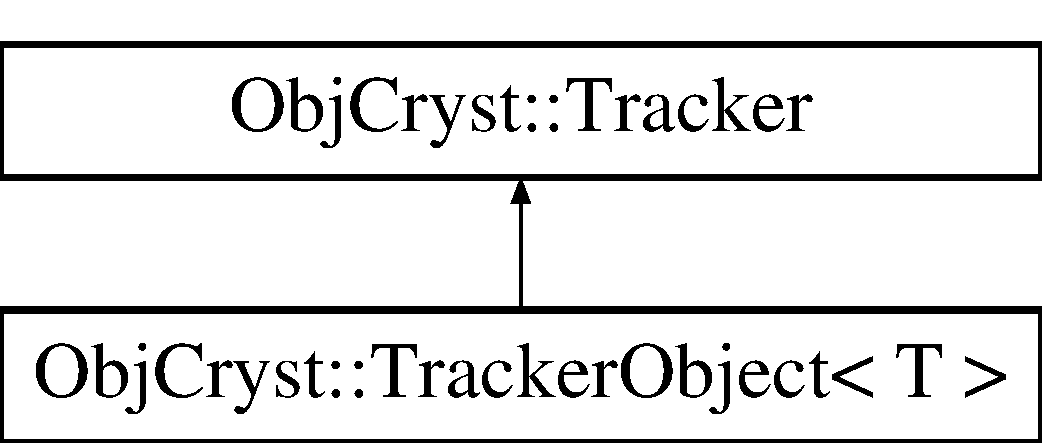
\includegraphics[height=2.000000cm]{a00113}
\end{center}
\end{figure}
\subsubsection*{Public Member Functions}
\begin{DoxyCompactItemize}
\item 
{\bfseries T\-O\-F\-Corr} (const {\bf Scattering\-Data} \&data)\label{a00113_afceb96fa351306b6bb3ca787dc56d5fc}

\item 
virtual const string \& {\bf Get\-Name} () const \label{a00113_a6638348a144ef78b7d40448869c8c220}

\begin{DoxyCompactList}\small\item\em Get the name of this object. \end{DoxyCompactList}\item 
virtual const string \& {\bf Get\-Class\-Name} () const \label{a00113_a9eecdda6f5d0ae119334e54043d1d7d6}

\begin{DoxyCompactList}\small\item\em Get the name of the class. \end{DoxyCompactList}\end{DoxyCompactItemize}
\subsubsection*{Protected Member Functions}
\begin{DoxyCompactItemize}
\item 
virtual void {\bf Calc\-Corr} () const \label{a00113_ae0a0c31d2edc029708722f00e05a5edf}

\begin{DoxyCompactList}\small\item\em Do the computation of corrected intensities. \end{DoxyCompactList}\end{DoxyCompactItemize}
\subsubsection*{Additional Inherited Members}


\subsubsection{Detailed Description}
Time-\/\-Of-\/\-Flight Correction. 

$ T = d^4\sin(\theta) $

The  angle of the detector is ignored, as it is just a scale factor. 

The documentation for this class was generated from the following file\-:\begin{DoxyCompactItemize}
\item 
Scattering\-Corr.\-h\end{DoxyCompactItemize}

\subsection{Obj\+Cryst\+:\+:Tracker\+Object$<$ T $>$ Class Template Reference}
\label{a00114}\index{Obj\+Cryst\+::\+Tracker\+Object$<$ T $>$@{Obj\+Cryst\+::\+Tracker\+Object$<$ T $>$}}


\doxyref{Tracker}{p.}{a00113} for objects (\doxyref{Refinable\+Obj}{p.}{a00077}, \doxyref{Crystal}{p.}{a00026}, \doxyref{Powder\+Pattern}{p.}{a00068}, Ref\+Par,...)  


Inheritance diagram for Obj\+Cryst\+:\+:Tracker\+Object$<$ T $>$\+:\begin{figure}[H]
\begin{center}
\leavevmode
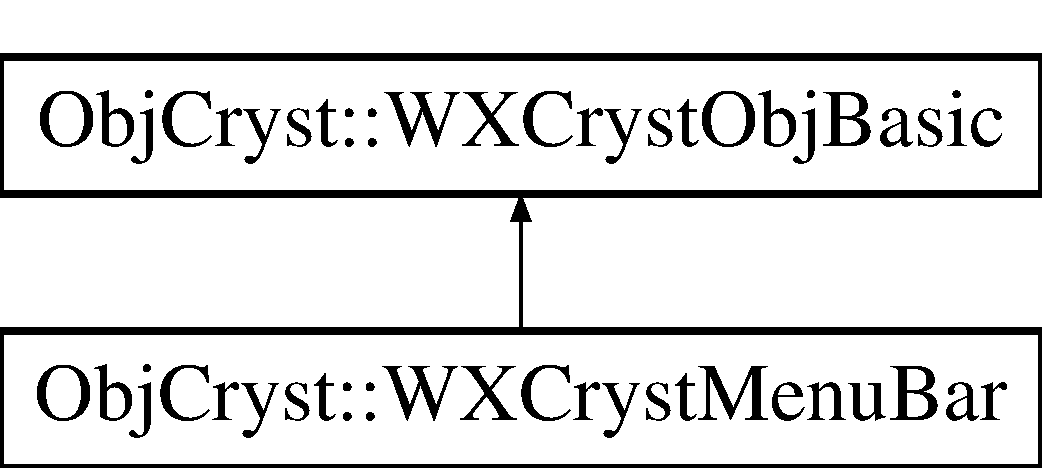
\includegraphics[height=2.000000cm]{a00114}
\end{center}
\end{figure}
\subsubsection*{Public Member Functions}
\begin{DoxyCompactItemize}
\item 
{\bfseries Tracker\+Object} (const std\+::string \&name, const T \&obj, R\+E\+A\+L(T\+::$\ast$f)() const)\label{a00114_a2309c151aec16dfac6d851f5dd531504}

\end{DoxyCompactItemize}
\subsubsection*{Private Member Functions}
\begin{DoxyCompactItemize}
\item 
R\+E\+A\+L {\bfseries Read\+Value} ()\label{a00114_a7e55a34fdcfedb2c6c8a671332a6fc7a}

\end{DoxyCompactItemize}
\subsubsection*{Private Attributes}
\begin{DoxyCompactItemize}
\item 
const T $\ast$ {\bfseries mp\+Obj}\label{a00114_af3365fd691f602db752df66aafbf5520}

\item 
R\+E\+A\+L(T\+::$\ast$ {\bfseries mfp} )() const \label{a00114_a5179813fa67eb55033ac57f1dcd02eb9}

\end{DoxyCompactItemize}
\subsubsection*{Additional Inherited Members}


\subsubsection{Detailed Description}
\subsubsection*{template$<$class T$>$class Obj\+Cryst\+::\+Tracker\+Object$<$ T $>$}

\doxyref{Tracker}{p.}{a00113} for objects (\doxyref{Refinable\+Obj}{p.}{a00077}, \doxyref{Crystal}{p.}{a00026}, \doxyref{Powder\+Pattern}{p.}{a00068}, Ref\+Par,...) 



The documentation for this class was generated from the following file\+:\begin{DoxyCompactItemize}
\item 
Tracker.\+h\end{DoxyCompactItemize}

\subsection{Obj\-Cryst\-:\-:Space\-Group\-:\-:T\-Rx Struct Reference}
\label{a00115}\index{Obj\-Cryst\-::\-Space\-Group\-::\-T\-Rx@{Obj\-Cryst\-::\-Space\-Group\-::\-T\-Rx}}


Struct to store trans matrix.  


\subsubsection*{Public Attributes}
\begin{DoxyCompactItemize}
\item 
R\-E\-A\-L {\bfseries tr} [3]\label{a00115_a3a74f496e2afd6b62644789eae6a0a61}

\end{DoxyCompactItemize}


\subsubsection{Detailed Description}
Struct to store trans matrix. 

The documentation for this struct was generated from the following file\-:\begin{DoxyCompactItemize}
\item 
Space\-Group.\-h\end{DoxyCompactItemize}

\subsection{Obj\-Cryst\-:\-:Space\-Group\-:\-:T\-Rx Struct Reference}
\label{a00116}\index{Obj\-Cryst\-::\-Space\-Group\-::\-T\-Rx@{Obj\-Cryst\-::\-Space\-Group\-::\-T\-Rx}}


Struct to store trans matrix.  


\subsubsection*{Public Attributes}
\begin{DoxyCompactItemize}
\item 
R\-E\-A\-L {\bfseries tr} [3]\label{a00116_a3a74f496e2afd6b62644789eae6a0a61}

\end{DoxyCompactItemize}


\subsubsection{Detailed Description}
Struct to store trans matrix. 

The documentation for this struct was generated from the following file\-:\begin{DoxyCompactItemize}
\item 
Space\-Group.\-h\end{DoxyCompactItemize}

\subsection{Obj\+Cryst\+:\+:W\+X\+Atom Class Reference}
\label{a00117}\index{Obj\+Cryst\+::\+W\+X\+Atom@{Obj\+Cryst\+::\+W\+X\+Atom}}


wx\+Cryst class for Atoms  


Inheritance diagram for Obj\+Cryst\+:\+:W\+X\+Atom\+:\begin{figure}[H]
\begin{center}
\leavevmode
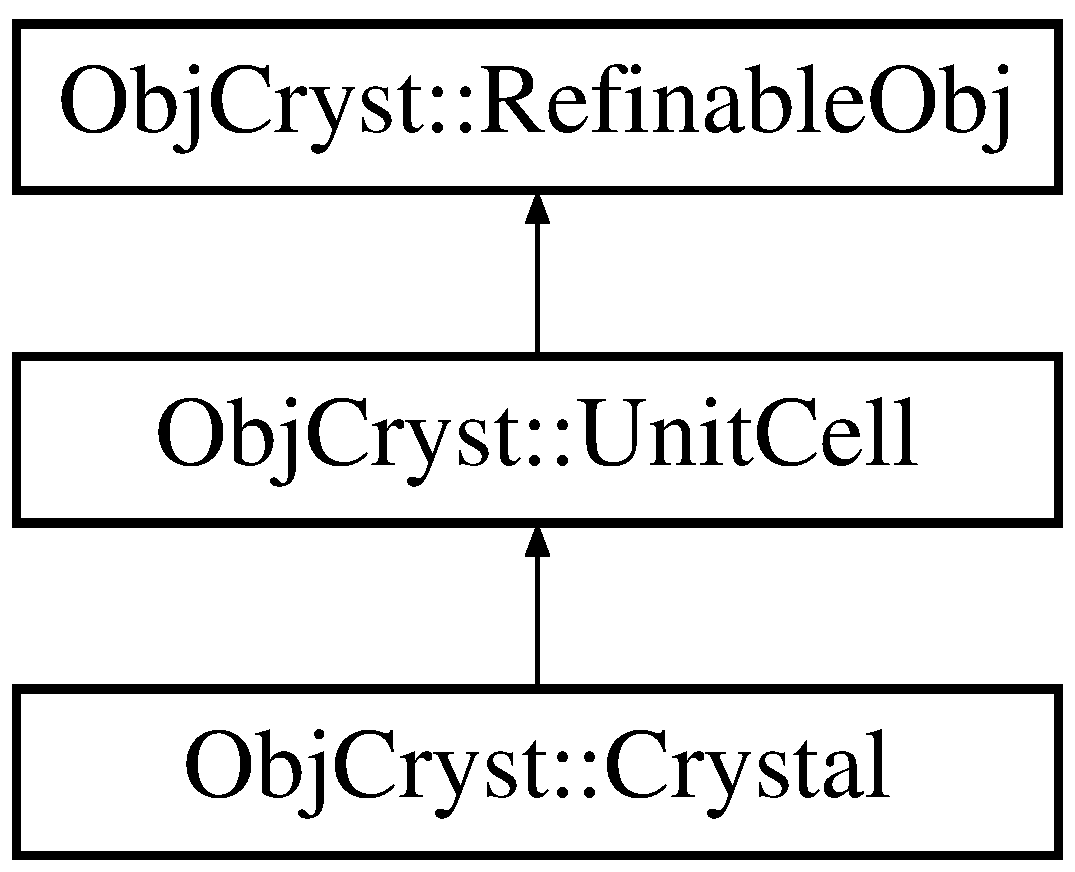
\includegraphics[height=5.000000cm]{a00117}
\end{center}
\end{figure}
\subsubsection*{Public Member Functions}
\begin{DoxyCompactItemize}
\item 
{\bfseries W\+X\+Atom} (wx\+Window $\ast$parent, {\bf Atom} $\ast$)\label{a00117_ad5013fde76bd65b8327976ee3d7b4538}

\item 
void {\bfseries On\+Change\+Scatt\+Pow} (wx\+Command\+Event \&W\+X\+U\+N\+U\+S\+E\+D(event))\label{a00117_a761d4b22d56c314568884ce001ae53d5}

\item 
virtual void {\bf Update\+U\+I} (const bool mutexlock=false)
\begin{DoxyCompactList}\small\item\em Update the User Interface, if necessary. \end{DoxyCompactList}\end{DoxyCompactItemize}
\subsubsection*{Private Attributes}
\begin{DoxyCompactItemize}
\item 
{\bf Atom} $\ast$ {\bfseries mp\+Atom}\label{a00117_ab4e8f3bee82f37e9ba24138d6015df04}

\item 
{\bf W\+X\+Field\+Choice} $\ast$ {\bfseries mp\+Field\+Scatt\+Power}\label{a00117_a9dd98ddab95fa288885099d719d22084}

\end{DoxyCompactItemize}
\subsubsection*{Additional Inherited Members}


\subsubsection{Detailed Description}
wx\+Cryst class for Atoms 

\subsubsection{Member Function Documentation}
\index{Obj\+Cryst\+::\+W\+X\+Atom@{Obj\+Cryst\+::\+W\+X\+Atom}!Update\+U\+I@{Update\+U\+I}}
\index{Update\+U\+I@{Update\+U\+I}!Obj\+Cryst\+::\+W\+X\+Atom@{Obj\+Cryst\+::\+W\+X\+Atom}}
\paragraph[{Update\+U\+I}]{\setlength{\rightskip}{0pt plus 5cm}virtual void Obj\+Cryst\+::\+W\+X\+Atom\+::\+Update\+U\+I (
\begin{DoxyParamCaption}
\item[{const bool}]{mutexlock = {\ttfamily false}}
\end{DoxyParamCaption}
)\hspace{0.3cm}{\ttfamily [virtual]}}\label{a00117_a5509a746fb1a6d918b6cbde8453d6a44}


Update the User Interface, if necessary. 


\begin{DoxyParams}{Parameters}
{\em mutexlock} & if true, a Mutex will be used to lock the data shared between main and background thread.\\
\hline
\end{DoxyParams}
The idea is to only use a few Mutexes to lock data from the top objects (wx\+Refinable\+Obj,...), when calling \doxyref{Cryst\+Update()}{p.}{a00149_a13e4f37ac098de756b27cdb91d6a0551} and \doxyref{Update\+U\+I()}{p.}{a00117_a5509a746fb1a6d918b6cbde8453d6a44}. As sub-\/objects (\doxyref{W\+X\+Field}{p.}{a00125},...) are only updated from within a top object, the mutex lock in the top object will also lock the data in the sub-\/objects. 

Reimplemented from {\bf Obj\+Cryst\+::\+W\+X\+Refinable\+Obj} \doxyref{}{p.}{a00149_a19a1d057eecafd48710d9a3b770c1b28}.



The documentation for this class was generated from the following file\+:\begin{DoxyCompactItemize}
\item 
wx\+Atom.\+h\end{DoxyCompactItemize}

\subsection{Obj\-Cryst\-:\-:W\-X\-C\-R\-Y\-S\-T\-\_\-\-I\-D Class Reference}
\label{a00118}\index{Obj\-Cryst\-::\-W\-X\-C\-R\-Y\-S\-T\-\_\-\-I\-D@{Obj\-Cryst\-::\-W\-X\-C\-R\-Y\-S\-T\-\_\-\-I\-D}}


Class to automatically assign a unique wx\-I\-D to each window.  


\subsubsection*{Public Member Functions}
\begin{DoxyCompactItemize}
\item 
{\bfseries operator long} ()\label{a00118_ad556605a5923122932a3425ca70dea59}

\end{DoxyCompactItemize}
\subsubsection*{Private Attributes}
\begin{DoxyCompactItemize}
\item 
long {\bfseries m\-Index}\label{a00118_ac93773bc8d556678497dde9ac2af6f60}

\end{DoxyCompactItemize}
\subsubsection*{Static Private Attributes}
\begin{DoxyCompactItemize}
\item 
static long {\bfseries m\-Counter}\label{a00118_aff3ad64b44e0d2193c6a4269026cce61}

\end{DoxyCompactItemize}


\subsubsection{Detailed Description}
Class to automatically assign a unique wx\-I\-D to each window. 



The documentation for this class was generated from the following file\-:\begin{DoxyCompactItemize}
\item 
wx\-Cryst.\-h\end{DoxyCompactItemize}

\subsection{ObjCryst::WXFieldChoice Class Reference}
\label{a00119}\index{ObjCryst::WXFieldChoice@{ObjCryst::WXFieldChoice}}


Class to pick one choice.  
Inheritance diagram for ObjCryst::WXFieldChoice::\begin{figure}[H]
\begin{center}
\leavevmode
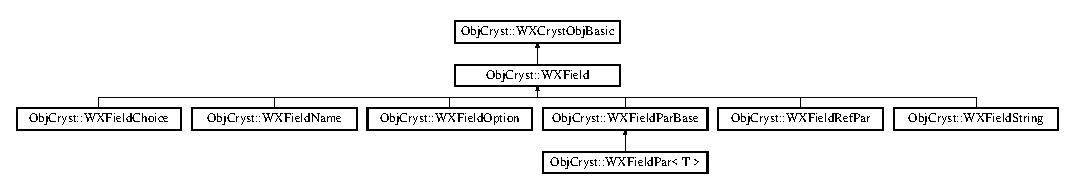
\includegraphics[height=3cm]{a00119}
\end{center}
\end{figure}
\subsubsection*{Public Member Functions}
\begin{DoxyCompactItemize}
\item 
{\bf WXFieldChoice} (wxWindow $\ast$parent, const int field\_\-id, const string \&name, const int hsize=80)\label{a00119_a1f2515335651539ee3a9b2cfc331f447}

\begin{DoxyCompactList}\small\item\em Constructor. \item\end{DoxyCompactList}\item 
virtual void {\bf CrystUpdate} (const bool updateUI=false, const bool mutexlock=false)\label{a00119_ade00cc3852045daceaab7f0eacba296a}

\begin{DoxyCompactList}\small\item\em Does nothing. \item\end{DoxyCompactList}\item 
virtual void {\bf UpdateUI} (const bool mutexlock=false)\label{a00119_a5cbdea12ea798037dd2da13fe53220f2}

\begin{DoxyCompactList}\small\item\em Does nothing. \item\end{DoxyCompactList}\item 
void {\bf Revert} ()
\begin{DoxyCompactList}\small\item\em After a user entry, this allows to go back to the last value, if for some reason the entry was rejected (because the object is currently busy, . \item\end{DoxyCompactList}\item 
void {\bf SetValue} (const string \&)\label{a00119_aae6b6916aaa6881c36aa543a05c68726}

\begin{DoxyCompactList}\small\item\em Used by the owner to change the name of the choice. \item\end{DoxyCompactList}\item 
virtual void {\bf ValidateUserInput} ()\label{a00119_a614c78cfd612074a7ac9474a6614bb89}

\begin{DoxyCompactList}\small\item\em Unnecessary here. Any change is immediately taken into account. \item\end{DoxyCompactList}\end{DoxyCompactItemize}
\subsubsection*{Protected Attributes}
\begin{DoxyCompactItemize}
\item 
wxButton $\ast$ {\bf mpButton}\label{a00119_a9b58dd176b85093cdda849d0cb041e5f}

\begin{DoxyCompactList}\small\item\em The button to be clicked to change the value. \item\end{DoxyCompactList}\end{DoxyCompactItemize}


\subsubsection{Detailed Description}
Class to pick one choice. .. Choice change/update is handled by the \doxyref{WXCrystObj}{p.}{a00114} owner, who should grab the incoming event. Useful, for example, to change the scattering power associated to an atom. 

\subsubsection{Member Function Documentation}
\index{ObjCryst::WXFieldChoice@{ObjCryst::WXFieldChoice}!Revert@{Revert}}
\index{Revert@{Revert}!ObjCryst::WXFieldChoice@{ObjCryst::WXFieldChoice}}
\paragraph[{Revert}]{\setlength{\rightskip}{0pt plus 5cm}void ObjCryst::WXFieldChoice::Revert ()\hspace{0.3cm}{\ttfamily  [virtual]}}\hfill\label{a00119_a3b923575bb9d616bd9c80a7929d0a388}


After a user entry, this allows to go back to the last value, if for some reason the entry was rejected (because the object is currently busy, . ..) 

Implements {\bf ObjCryst::WXField} \doxyref{}{p.}{a00118_a178d6d770d1e3adfa02e27da94b2dffa}.

The documentation for this class was generated from the following file:\begin{DoxyCompactItemize}
\item 
wxCryst.h\end{DoxyCompactItemize}

\subsection{Obj\-Cryst\-:\-:W\-X\-Cryst\-Menu\-Bar Class Reference}
\label{a00120}\index{Obj\-Cryst\-::\-W\-X\-Cryst\-Menu\-Bar@{Obj\-Cryst\-::\-W\-X\-Cryst\-Menu\-Bar}}


Our own local menu bar, using buttons and Popup menus.  


Inheritance diagram for Obj\-Cryst\-:\-:W\-X\-Cryst\-Menu\-Bar\-:\begin{figure}[H]
\begin{center}
\leavevmode
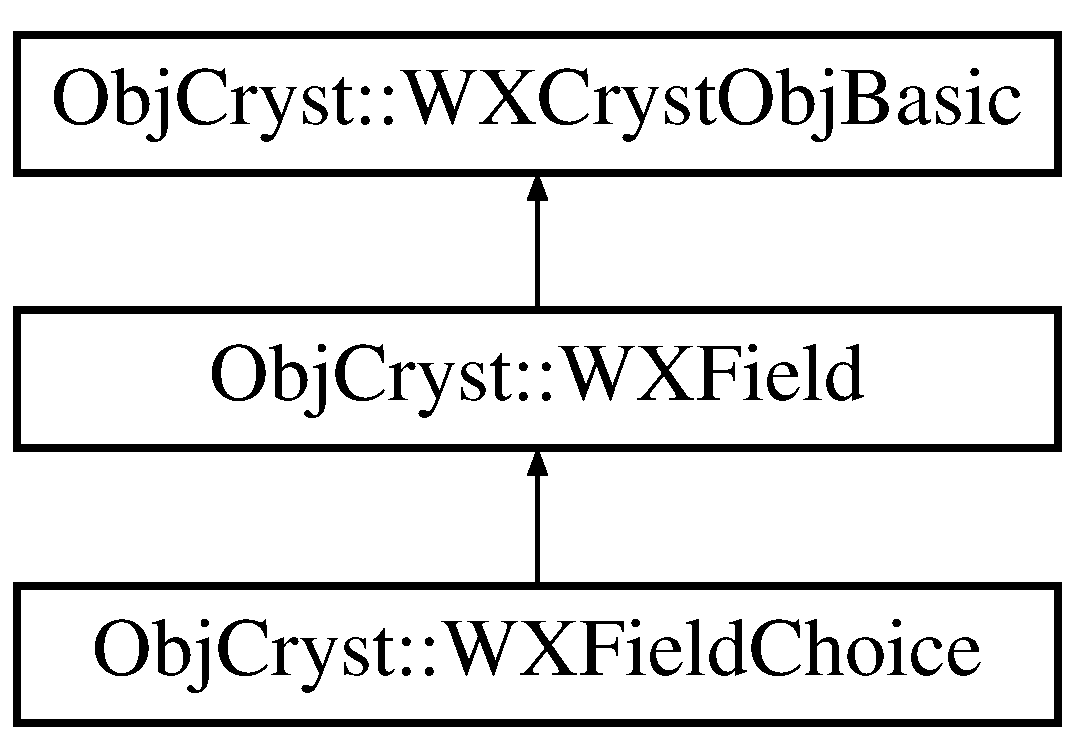
\includegraphics[height=2.000000cm]{a00120}
\end{center}
\end{figure}
\subsubsection*{Public Member Functions}
\begin{DoxyCompactItemize}
\item 
{\bf W\-X\-Cryst\-Menu\-Bar} (wx\-Window $\ast$parent, {\bf W\-X\-Cryst\-Obj} $\ast$owner)\label{a00120_aaa68b57dce657185fe3a93c19ecc648a}

\begin{DoxyCompactList}\small\item\em Ctor. \end{DoxyCompactList}\item 
void {\bf Add\-Menu} (const string \&name, const int menu\-Id, const string \&help=\char`\"{}\char`\"{})\label{a00120_a99b2ca415d2bb4b670433557b1d42a5d}

\begin{DoxyCompactList}\small\item\em Add a menu. \end{DoxyCompactList}\item 
wx\-Menu \& {\bf Get\-Menu} (const int menu\-Id)\label{a00120_a9a378d85bab72be5faec773730df4505}

\begin{DoxyCompactList}\small\item\em Get access to a menu. \end{DoxyCompactList}\item 
void {\bf Add\-Menu\-Item} (const int menu\-Id, int id, const string \&item, const string \&help=\char`\"{}\char`\"{}, const bool checkable=false)\label{a00120_a689d06fe301f17b5e8940286d107340a}

\begin{DoxyCompactList}\small\item\em Add an entry to a menu. \end{DoxyCompactList}\item 
void {\bf Add\-Menu\-Item} (const int menu\-Id, int id, const wx\-String \&item, wx\-Menu $\ast$sub\-Menu, const wx\-String \&help\-String=\-\_\-\-T(\char`\"{}\char`\"{}))\label{a00120_a8d8e212441d2df35499e13bc38c7c463}

\begin{DoxyCompactList}\small\item\em Add a sub-\/menu to a menu. \end{DoxyCompactList}\item 
virtual void {\bf Cryst\-Update} (const bool update\-U\-I=false, const bool mutexlock=false)
\begin{DoxyCompactList}\small\item\em Get new values to be displayed from the underlying object, and raise flag if an U\-I update is necessary. \end{DoxyCompactList}\item 
virtual void {\bf Update\-U\-I} (const bool mutexlock=false)
\begin{DoxyCompactList}\small\item\em Update the User Interface, if necessary. \end{DoxyCompactList}\item 
void {\bf On\-Popup\-Menu} (wx\-Command\-Event \&event)\label{a00120_ade8539411ad2badf7ca0d84c982d1e1e}

\begin{DoxyCompactList}\small\item\em Event handler to popu the menu when the button is clicked. \end{DoxyCompactList}\item 
virtual void {\bf Set\-Tool\-Tip} (const wx\-String \&tip, long menu=0)\label{a00120_ad0ddf5302f5425ffcdcd4bf3681987dd}

\begin{DoxyCompactList}\small\item\em Set tooltip for each menu. \end{DoxyCompactList}\end{DoxyCompactItemize}
\subsubsection*{Protected Attributes}
\begin{DoxyCompactItemize}
\item 
wx\-Box\-Sizer $\ast$ {\bf mp\-Sizer}\label{a00120_a082b747b0a157df1dbe86349450f3f7a}

\begin{DoxyCompactList}\small\item\em The sizer of the menu. \end{DoxyCompactList}\item 
std\-::map$<$ long, pair$<$ wx\-Menu \\*
$\ast$, wx\-Button $\ast$ $>$ $>$ {\bf mvp\-Menu}\label{a00120_a73b92cea8b7a55c69d3c552771505560}

\begin{DoxyCompactList}\small\item\em List of menus, first is the menu Id and second is a pair of $<$pointer to the menu, pointer to the button of the menu$>$ \end{DoxyCompactList}\end{DoxyCompactItemize}


\subsubsection{Detailed Description}
Our own local menu bar, using buttons and Popup menus. 

\subsubsection{Member Function Documentation}
\index{Obj\-Cryst\-::\-W\-X\-Cryst\-Menu\-Bar@{Obj\-Cryst\-::\-W\-X\-Cryst\-Menu\-Bar}!Cryst\-Update@{Cryst\-Update}}
\index{Cryst\-Update@{Cryst\-Update}!ObjCryst::WXCrystMenuBar@{Obj\-Cryst\-::\-W\-X\-Cryst\-Menu\-Bar}}
\paragraph[{Cryst\-Update}]{\setlength{\rightskip}{0pt plus 5cm}virtual void Obj\-Cryst\-::\-W\-X\-Cryst\-Menu\-Bar\-::\-Cryst\-Update (
\begin{DoxyParamCaption}
\item[{const bool}]{update\-U\-I = {\ttfamily false}, }
\item[{const bool}]{mutexlock = {\ttfamily false}}
\end{DoxyParamCaption}
)\hspace{0.3cm}{\ttfamily [virtual]}}\label{a00120_ac0c3dead0da352d0c7e439508bc40303}


Get new values to be displayed from the underlying object, and raise flag if an U\-I update is necessary. 

The actual G\-U\-I update is not made here. \doxyref{Update\-U\-I()}{p.}{a00120_acc23d478cb50225e17fb5b6dc29fce7b} should be called separately, from the main thread.


\begin{DoxyParams}{Parameters}
{\em update\-U\-I} & if true, this will call Update\-U\-I, either directly (if in the main thread), or by sending a message. \\
\hline
{\em mutexlock} & if true, a Mutex will be used to lock the data shared between main and background thread. The idea is to only use a few Mutexes to lock data from the top objects (wx\-Refinable\-Obj,...), when calling \doxyref{Cryst\-Update()}{p.}{a00120_ac0c3dead0da352d0c7e439508bc40303} and \doxyref{Update\-U\-I()}{p.}{a00120_acc23d478cb50225e17fb5b6dc29fce7b}. As sub-\/objects (\doxyref{W\-X\-Field}{p.}{a00125},...) are only updated from within a top object, the mutex lock in the top object will also lock the data in the sub-\/objects. \\
\hline
\end{DoxyParams}


Implements {\bf Obj\-Cryst\-::\-W\-X\-Cryst\-Obj\-Basic} \doxyref{}{p.}{a00122_a7ac00ae2ae28f1a6fa26e6fa571186b6}.

\index{Obj\-Cryst\-::\-W\-X\-Cryst\-Menu\-Bar@{Obj\-Cryst\-::\-W\-X\-Cryst\-Menu\-Bar}!Update\-U\-I@{Update\-U\-I}}
\index{Update\-U\-I@{Update\-U\-I}!ObjCryst::WXCrystMenuBar@{Obj\-Cryst\-::\-W\-X\-Cryst\-Menu\-Bar}}
\paragraph[{Update\-U\-I}]{\setlength{\rightskip}{0pt plus 5cm}virtual void Obj\-Cryst\-::\-W\-X\-Cryst\-Menu\-Bar\-::\-Update\-U\-I (
\begin{DoxyParamCaption}
\item[{const bool}]{mutexlock = {\ttfamily false}}
\end{DoxyParamCaption}
)\hspace{0.3cm}{\ttfamily [virtual]}}\label{a00120_acc23d478cb50225e17fb5b6dc29fce7b}


Update the User Interface, if necessary. 


\begin{DoxyParams}{Parameters}
{\em mutexlock} & if true, a Mutex will be used to lock the data shared between main and background thread.\\
\hline
\end{DoxyParams}
The idea is to only use a few Mutexes to lock data from the top objects (wx\-Refinable\-Obj,...), when calling \doxyref{Cryst\-Update()}{p.}{a00120_ac0c3dead0da352d0c7e439508bc40303} and \doxyref{Update\-U\-I()}{p.}{a00120_acc23d478cb50225e17fb5b6dc29fce7b}. As sub-\/objects (\doxyref{W\-X\-Field}{p.}{a00125},...) are only updated from within a top object, the mutex lock in the top object will also lock the data in the sub-\/objects. 

Implements {\bf Obj\-Cryst\-::\-W\-X\-Cryst\-Obj\-Basic} \doxyref{}{p.}{a00122_a3818940b7031ff7e45cf2178c4a99c90}.



The documentation for this class was generated from the following file\-:\begin{DoxyCompactItemize}
\item 
wx\-Cryst.\-h\end{DoxyCompactItemize}

\subsection{Obj\-Cryst\-:\-:W\-X\-Cryst\-Obj Class Reference}
\label{a00121}\index{Obj\-Cryst\-::\-W\-X\-Cryst\-Obj@{Obj\-Cryst\-::\-W\-X\-Cryst\-Obj}}


Base class for all displayed \doxyref{Obj\-Cryst}{p.}{a00177} objects (with a title, and a sizer to stack objects).  


Inheritance diagram for Obj\-Cryst\-:\-:W\-X\-Cryst\-Obj\-:\begin{figure}[H]
\begin{center}
\leavevmode
\includegraphics[height=8.369565cm]{a00121}
\end{center}
\end{figure}
\subsubsection*{Public Member Functions}
\begin{DoxyCompactItemize}
\item 
{\bf W\-X\-Cryst\-Obj} (wx\-Window $\ast$parent, int orient=wx\-H\-O\-R\-I\-Z\-O\-N\-T\-A\-L, bool show\-Name=true)\label{a00121_aee6a4d5c3a1dfa315e5520f56621c153}

\begin{DoxyCompactList}\small\item\em Constructor, with a. \end{DoxyCompactList}\item 
void {\bf On\-Toggle\-Collapse} (wx\-Command\-Event \&W\-X\-U\-N\-U\-S\-E\-D(event))
\begin{DoxyCompactList}\small\item\em Only display the title, and collapse everything else. \end{DoxyCompactList}\item 
virtual bool {\bf On\-Change\-Name} (const int id)=0
\begin{DoxyCompactList}\small\item\em When a \doxyref{W\-X\-Field\-Name}{p.}{a00127} has been changed by the user, it is handled here. \end{DoxyCompactList}\item 
virtual void {\bf Cryst\-Update} (const bool update\-U\-I=false, const bool mutexlock=false)
\begin{DoxyCompactList}\small\item\em Get new values to be displayed from the underlying object, and raise flag if an U\-I update is necessary. \end{DoxyCompactList}\item 
virtual void {\bf Update\-U\-I} (const bool mutexlock=false)
\begin{DoxyCompactList}\small\item\em Update the User Interface, if necessary. \end{DoxyCompactList}\item 
virtual void {\bfseries On\-Enable} (wx\-Update\-U\-I\-Event \&event)\label{a00121_a862e490ea63c3f4e81e727dd76c11f50}

\item 
virtual bool {\bfseries Enable} (bool enable)\label{a00121_adb1428e6b8fea322ec93212af80d17d3}

\item 
virtual void {\bf Bottom\-Layout} ({\bf W\-X\-Cryst\-Obj\-Basic} $\ast$p\-Child)
\begin{DoxyCompactList}\small\item\em Ask for a new Layout with recalculated size hints, because a child has been changed or added. \end{DoxyCompactList}\item 
virtual void {\bf Add\-Child} ({\bf W\-X\-Cryst\-Obj\-Basic} $\ast$p\-Child, bool do\-Bottom\-Layout=true)
\begin{DoxyCompactList}\small\item\em Notify that a new children has been added, also adding it to the correct sizer (which can be the top sizer or not). \end{DoxyCompactList}\end{DoxyCompactItemize}
\subsubsection*{Protected Attributes}
\begin{DoxyCompactItemize}
\item 
wx\-Box\-Sizer $\ast$ {\bf mp\-Top\-Sizer}\label{a00121_aaa27c0ed63bd119b55b884dc274c71bc}

\begin{DoxyCompactList}\small\item\em Top sizer including the title and \doxyref{W\-X\-Cryst\-Obj\-::mp\-Sizer}{p.}{a00121_a0fcc77bbdc5c4c3e191f96e15e82ef86}. \end{DoxyCompactList}\item 
wx\-Box\-Sizer $\ast$ {\bf mp\-Sizer}\label{a00121_a0fcc77bbdc5c4c3e191f96e15e82ef86}

\begin{DoxyCompactList}\small\item\em Sizer including all sub-\/objects. \end{DoxyCompactList}\item 
{\bf W\-X\-Field\-Name} $\ast$ {\bf mp\-W\-X\-Title}\label{a00121_a047ca586b293087e62eaa2054ce6164e}

\begin{DoxyCompactList}\small\item\em The title. \end{DoxyCompactList}\item 
bool {\bf m\-Is\-Expanded}\label{a00121_a0ad5527d3992a9aa86b1f1475c213521}

\begin{DoxyCompactList}\small\item\em To be used for collapsing the sub-\/objects. \end{DoxyCompactList}\item 
{\bf W\-X\-Cryst\-Obj\-Basic\-List} {\bf m\-List}\label{a00121_a2ec7c27e1a75da178e402c6166301126}

\begin{DoxyCompactList}\small\item\em All windows but the title and collapse button are in this list. \end{DoxyCompactList}\item 
wx\-Button $\ast$ {\bf mp\-Collapse\-Button}\label{a00121_abdcafc600137d8c8603dc5af76476eea}

\begin{DoxyCompactList}\small\item\em The collapse button. \end{DoxyCompactList}\end{DoxyCompactItemize}


\subsubsection{Detailed Description}
Base class for all displayed \doxyref{Obj\-Cryst}{p.}{a00177} objects (with a title, and a sizer to stack objects). 

A button (which should be used to collapse the object) is used to create an indentation for the sub-\/objects.

\begin{DoxyRefDesc}{Todo}
\item[{\bf Todo}]Allow the objects to be collabsable. The difficulty is that even if the object is not shown, it is not removed by the Sizer as long as it is not deleted... Needs some testing ! Otherwise it would also be possible to delete and re-\/create sub-\/objects when collapsing, but that would be more difficult. \end{DoxyRefDesc}


\subsubsection{Member Function Documentation}
\index{Obj\-Cryst\-::\-W\-X\-Cryst\-Obj@{Obj\-Cryst\-::\-W\-X\-Cryst\-Obj}!Add\-Child@{Add\-Child}}
\index{Add\-Child@{Add\-Child}!ObjCryst::WXCrystObj@{Obj\-Cryst\-::\-W\-X\-Cryst\-Obj}}
\paragraph[{Add\-Child}]{\setlength{\rightskip}{0pt plus 5cm}virtual void Obj\-Cryst\-::\-W\-X\-Cryst\-Obj\-::\-Add\-Child (
\begin{DoxyParamCaption}
\item[{{\bf W\-X\-Cryst\-Obj\-Basic} $\ast$}]{p\-Child, }
\item[{bool}]{do\-Bottom\-Layout = {\ttfamily true}}
\end{DoxyParamCaption}
)\hspace{0.3cm}{\ttfamily [virtual]}}\label{a00121_a0e0790010b9be47e533998a61f27fa1a}


Notify that a new children has been added, also adding it to the correct sizer (which can be the top sizer or not). 


\begin{DoxyParams}{Parameters}
{\em do\-Bottom\-Layout} & ask for a new Layout of the window and of its parents. \\
\hline
\end{DoxyParams}


Reimplemented from {\bf Obj\-Cryst\-::\-W\-X\-Cryst\-Obj\-Basic} \doxyref{}{p.}{a00122_ae346606a6dbb6aeffe89fc16de380b81}.

\index{Obj\-Cryst\-::\-W\-X\-Cryst\-Obj@{Obj\-Cryst\-::\-W\-X\-Cryst\-Obj}!Bottom\-Layout@{Bottom\-Layout}}
\index{Bottom\-Layout@{Bottom\-Layout}!ObjCryst::WXCrystObj@{Obj\-Cryst\-::\-W\-X\-Cryst\-Obj}}
\paragraph[{Bottom\-Layout}]{\setlength{\rightskip}{0pt plus 5cm}virtual void Obj\-Cryst\-::\-W\-X\-Cryst\-Obj\-::\-Bottom\-Layout (
\begin{DoxyParamCaption}
\item[{{\bf W\-X\-Cryst\-Obj\-Basic} $\ast$}]{p\-Child}
\end{DoxyParamCaption}
)\hspace{0.3cm}{\ttfamily [virtual]}}\label{a00121_a8fcadf77f9216819c62384d0c03bd710}


Ask for a new Layout with recalculated size hints, because a child has been changed or added. 


\begin{DoxyParams}{Parameters}
{\em p\-Child} & the modified child. If null, this will mean we are asking for a new layout of the window itself (useful when a sub-\/window is deleted). \\
\hline
\end{DoxyParams}


Reimplemented from {\bf Obj\-Cryst\-::\-W\-X\-Cryst\-Obj\-Basic} \doxyref{}{p.}{a00122_afbd0ece297950eda664fa819c240a318}.

\index{Obj\-Cryst\-::\-W\-X\-Cryst\-Obj@{Obj\-Cryst\-::\-W\-X\-Cryst\-Obj}!Cryst\-Update@{Cryst\-Update}}
\index{Cryst\-Update@{Cryst\-Update}!ObjCryst::WXCrystObj@{Obj\-Cryst\-::\-W\-X\-Cryst\-Obj}}
\paragraph[{Cryst\-Update}]{\setlength{\rightskip}{0pt plus 5cm}virtual void Obj\-Cryst\-::\-W\-X\-Cryst\-Obj\-::\-Cryst\-Update (
\begin{DoxyParamCaption}
\item[{const bool}]{update\-U\-I = {\ttfamily false}, }
\item[{const bool}]{mutexlock = {\ttfamily false}}
\end{DoxyParamCaption}
)\hspace{0.3cm}{\ttfamily [virtual]}}\label{a00121_a2e5de90ae4d1ca8feb65b88debf6d3cb}


Get new values to be displayed from the underlying object, and raise flag if an U\-I update is necessary. 

The actual G\-U\-I update is not made here. \doxyref{Update\-U\-I()}{p.}{a00121_a093c04eb7b70ff063b80427779c7c456} should be called separately, from the main thread.


\begin{DoxyParams}{Parameters}
{\em update\-U\-I} & if true, this will call Update\-U\-I, either directly (if in the main thread), or by sending a message. \\
\hline
{\em mutexlock} & if true, a Mutex will be used to lock the data shared between main and background thread. The idea is to only use a few Mutexes to lock data from the top objects (wx\-Refinable\-Obj,...), when calling \doxyref{Cryst\-Update()}{p.}{a00121_a2e5de90ae4d1ca8feb65b88debf6d3cb} and \doxyref{Update\-U\-I()}{p.}{a00121_a093c04eb7b70ff063b80427779c7c456}. As sub-\/objects (\doxyref{W\-X\-Field}{p.}{a00125},...) are only updated from within a top object, the mutex lock in the top object will also lock the data in the sub-\/objects. \\
\hline
\end{DoxyParams}


Implements {\bf Obj\-Cryst\-::\-W\-X\-Cryst\-Obj\-Basic} \doxyref{}{p.}{a00122_a7ac00ae2ae28f1a6fa26e6fa571186b6}.



Reimplemented in {\bf Obj\-Cryst\-::\-W\-X\-Powder\-Pattern\-Background} \doxyref{}{p.}{a00143_adacc1d5b1efe6eaf6a7a6a2d544c5e81}, {\bf Obj\-Cryst\-::\-W\-X\-Molecule} \doxyref{}{p.}{a00138_a4d8fe8698ddc741c34b613643dec87b0}, {\bf Obj\-Cryst\-::\-W\-X\-Refinable\-Obj} \doxyref{}{p.}{a00149_a13e4f37ac098de756b27cdb91d6a0551}, {\bf Obj\-Cryst\-::\-W\-X\-Crystal} \doxyref{}{p.}{a00119_a55d7dc41da5c6d4360609d2eac91f39b}, {\bf Obj\-Cryst\-::\-W\-X\-Optimization\-Obj} \doxyref{}{p.}{a00141_a440befb33ae526a51eb9a7f3d9739d3e}, {\bf Obj\-Cryst\-::\-W\-X\-Powder\-Pattern} \doxyref{}{p.}{a00142_a90f999b4aab7ed134db388c532b1d63e}, and {\bf Obj\-Cryst\-::\-W\-X\-Diffraction\-Single\-Crystal} \doxyref{}{p.}{a00124_a79a9bb91f352c12bfb3a1ebd60267cbc}.

\index{Obj\-Cryst\-::\-W\-X\-Cryst\-Obj@{Obj\-Cryst\-::\-W\-X\-Cryst\-Obj}!On\-Change\-Name@{On\-Change\-Name}}
\index{On\-Change\-Name@{On\-Change\-Name}!ObjCryst::WXCrystObj@{Obj\-Cryst\-::\-W\-X\-Cryst\-Obj}}
\paragraph[{On\-Change\-Name}]{\setlength{\rightskip}{0pt plus 5cm}virtual bool Obj\-Cryst\-::\-W\-X\-Cryst\-Obj\-::\-On\-Change\-Name (
\begin{DoxyParamCaption}
\item[{const int}]{id}
\end{DoxyParamCaption}
)\hspace{0.3cm}{\ttfamily [pure virtual]}}\label{a00121_a3736357599263df7e550790753c040a3}


When a \doxyref{W\-X\-Field\-Name}{p.}{a00127} has been changed by the user, it is handled here. 

This returns true if the value has been handled (for inheritance purposes). 

Implemented in {\bf Obj\-Cryst\-::\-W\-X\-Profile\-Double\-Exponential\-Pseudo\-Voigt} \doxyref{}{p.}{a00146_adbfe19fda83e06f57047c064dbdd6ba3}, {\bf Obj\-Cryst\-::\-W\-X\-Profile\-Pseudo\-Voigt} \doxyref{}{p.}{a00147_a6af548e3f77328ca30fb3a06a50fd40a}, {\bf Obj\-Cryst\-::\-W\-X\-Refinable\-Obj} \doxyref{}{p.}{a00149_ad784c1cb9ccb0d0e4ebfbc18a8dbbc19}, {\bf Obj\-Cryst\-::\-W\-X\-Registry$<$ T $>$} \doxyref{}{p.}{a00150_add68cfae172f6d78a3261927a5977474}, {\bf Obj\-Cryst\-::\-W\-X\-Registry$<$ Obj\-Cryst\-::\-Scatterer $>$} \doxyref{}{p.}{a00150_add68cfae172f6d78a3261927a5977474}, {\bf Obj\-Cryst\-::\-W\-X\-Registry$<$ Obj\-Cryst\-::\-Powder\-Pattern\-Component $>$} \doxyref{}{p.}{a00150_add68cfae172f6d78a3261927a5977474}, {\bf Obj\-Cryst\-::\-W\-X\-Registry$<$ Obj\-Cryst\-::\-Z\-Atom $>$} \doxyref{}{p.}{a00150_add68cfae172f6d78a3261927a5977474}, {\bf Obj\-Cryst\-::\-W\-X\-Registry$<$ Obj\-Cryst\-::\-Scattering\-Power $>$} \doxyref{}{p.}{a00150_add68cfae172f6d78a3261927a5977474}, {\bf Obj\-Cryst\-::\-W\-X\-Crystal} \doxyref{}{p.}{a00119_a7a15c2d1b5f5997ace336724fc396892}, {\bf Obj\-Cryst\-::\-W\-X\-Optimization\-Obj} \doxyref{}{p.}{a00141_a19a866ffdeaba16f73fe3af78dbffa58}, {\bf Obj\-Cryst\-::\-W\-X\-Scattering\-Power\-Atom} \doxyref{}{p.}{a00152_a99081b400737a5e28a7207c8c905f6d5}, and {\bf Obj\-Cryst\-::\-W\-X\-Scattering\-Power\-Sphere} \doxyref{}{p.}{a00153_a54f201d096de63b349e8979d69d6933a}.

\index{Obj\-Cryst\-::\-W\-X\-Cryst\-Obj@{Obj\-Cryst\-::\-W\-X\-Cryst\-Obj}!On\-Toggle\-Collapse@{On\-Toggle\-Collapse}}
\index{On\-Toggle\-Collapse@{On\-Toggle\-Collapse}!ObjCryst::WXCrystObj@{Obj\-Cryst\-::\-W\-X\-Cryst\-Obj}}
\paragraph[{On\-Toggle\-Collapse}]{\setlength{\rightskip}{0pt plus 5cm}void Obj\-Cryst\-::\-W\-X\-Cryst\-Obj\-::\-On\-Toggle\-Collapse (
\begin{DoxyParamCaption}
\item[{wx\-Command\-Event \&}]{W\-X\-U\-N\-U\-S\-E\-Devent}
\end{DoxyParamCaption}
)}\label{a00121_ae55c3091101cae5d79e5aacb77c48856}


Only display the title, and collapse everything else. 

\begin{DoxyRefDesc}{Bug}
\item[{\bf Bug}]\-: the windows do collapse, but the size of the window is not changed, so it is pretty useless so far... \end{DoxyRefDesc}
\index{Obj\-Cryst\-::\-W\-X\-Cryst\-Obj@{Obj\-Cryst\-::\-W\-X\-Cryst\-Obj}!Update\-U\-I@{Update\-U\-I}}
\index{Update\-U\-I@{Update\-U\-I}!ObjCryst::WXCrystObj@{Obj\-Cryst\-::\-W\-X\-Cryst\-Obj}}
\paragraph[{Update\-U\-I}]{\setlength{\rightskip}{0pt plus 5cm}virtual void Obj\-Cryst\-::\-W\-X\-Cryst\-Obj\-::\-Update\-U\-I (
\begin{DoxyParamCaption}
\item[{const bool}]{mutexlock = {\ttfamily false}}
\end{DoxyParamCaption}
)\hspace{0.3cm}{\ttfamily [virtual]}}\label{a00121_a093c04eb7b70ff063b80427779c7c456}


Update the User Interface, if necessary. 


\begin{DoxyParams}{Parameters}
{\em mutexlock} & if true, a Mutex will be used to lock the data shared between main and background thread.\\
\hline
\end{DoxyParams}
The idea is to only use a few Mutexes to lock data from the top objects (wx\-Refinable\-Obj,...), when calling \doxyref{Cryst\-Update()}{p.}{a00121_a2e5de90ae4d1ca8feb65b88debf6d3cb} and \doxyref{Update\-U\-I()}{p.}{a00121_a093c04eb7b70ff063b80427779c7c456}. As sub-\/objects (\doxyref{W\-X\-Field}{p.}{a00125},...) are only updated from within a top object, the mutex lock in the top object will also lock the data in the sub-\/objects. 

Implements {\bf Obj\-Cryst\-::\-W\-X\-Cryst\-Obj\-Basic} \doxyref{}{p.}{a00122_a3818940b7031ff7e45cf2178c4a99c90}.



Reimplemented in {\bf Obj\-Cryst\-::\-W\-X\-Powder\-Pattern\-Diffraction} \doxyref{}{p.}{a00144_a0f7d965eea526ddce53d5bda8487b3fa}, {\bf Obj\-Cryst\-::\-W\-X\-Powder\-Pattern\-Background} \doxyref{}{p.}{a00143_a11c6de5af2d72bcfc276838a2d62c32e}, {\bf Obj\-Cryst\-::\-W\-X\-Molecule} \doxyref{}{p.}{a00138_ae932cbbd6d7e55d319f1b4eb169c63ef}, {\bf Obj\-Cryst\-::\-W\-X\-Refinable\-Obj} \doxyref{}{p.}{a00149_a19a1d057eecafd48710d9a3b770c1b28}, {\bf Obj\-Cryst\-::\-W\-X\-Crystal} \doxyref{}{p.}{a00119_a62946717943682dc2ac07ea4584030f4}, {\bf Obj\-Cryst\-::\-W\-X\-Powder\-Pattern} \doxyref{}{p.}{a00142_aaeace05033eaea9499398825fc8244da}, {\bf Obj\-Cryst\-::\-W\-X\-Optimization\-Obj} \doxyref{}{p.}{a00141_adbaf395e3e68e7605da0805e0e6465a0}, {\bf Obj\-Cryst\-::\-W\-X\-Atom} \doxyref{}{p.}{a00117_a5509a746fb1a6d918b6cbde8453d6a44}, {\bf Obj\-Cryst\-::\-W\-X\-Diffraction\-Single\-Crystal} \doxyref{}{p.}{a00124_a6419580548c5f35434e0128b62f5b4e6}, {\bf Obj\-Cryst\-::\-W\-X\-Scattering\-Power\-Atom} \doxyref{}{p.}{a00152_a727146d4ecd5e1c4e5790a3eab0f0ace}, and {\bf Obj\-Cryst\-::\-W\-X\-Scattering\-Power\-Sphere} \doxyref{}{p.}{a00153_a95d4f9b618ffbd4885294806b12b066c}.



The documentation for this class was generated from the following file\-:\begin{DoxyCompactItemize}
\item 
wx\-Cryst.\-h\end{DoxyCompactItemize}

\subsection{Obj\-Cryst\-:\-:W\-X\-Cryst\-Obj Class Reference}
\label{a00122}\index{Obj\-Cryst\-::\-W\-X\-Cryst\-Obj@{Obj\-Cryst\-::\-W\-X\-Cryst\-Obj}}


Base class for all displayed \doxyref{Obj\-Cryst}{p.}{a00178} objects (with a title, and a sizer to stack objects).  


Inheritance diagram for Obj\-Cryst\-:\-:W\-X\-Cryst\-Obj\-:\begin{figure}[H]
\begin{center}
\leavevmode
\includegraphics[height=8.369565cm]{a00122}
\end{center}
\end{figure}
\subsubsection*{Public Member Functions}
\begin{DoxyCompactItemize}
\item 
{\bf W\-X\-Cryst\-Obj} (wx\-Window $\ast$parent, int orient=wx\-H\-O\-R\-I\-Z\-O\-N\-T\-A\-L, bool show\-Name=true)\label{a00122_aee6a4d5c3a1dfa315e5520f56621c153}

\begin{DoxyCompactList}\small\item\em Constructor, with a. \end{DoxyCompactList}\item 
void {\bf On\-Toggle\-Collapse} (wx\-Command\-Event \&W\-X\-U\-N\-U\-S\-E\-D(event))
\begin{DoxyCompactList}\small\item\em Only display the title, and collapse everything else. \end{DoxyCompactList}\item 
virtual bool {\bf On\-Change\-Name} (const int id)=0
\begin{DoxyCompactList}\small\item\em When a \doxyref{W\-X\-Field\-Name}{p.}{a00128} has been changed by the user, it is handled here. \end{DoxyCompactList}\item 
virtual void {\bf Cryst\-Update} (const bool update\-U\-I=false, const bool mutexlock=false)
\begin{DoxyCompactList}\small\item\em Get new values to be displayed from the underlying object, and raise flag if an U\-I update is necessary. \end{DoxyCompactList}\item 
virtual void {\bf Update\-U\-I} (const bool mutexlock=false)
\begin{DoxyCompactList}\small\item\em Update the User Interface, if necessary. \end{DoxyCompactList}\item 
virtual void {\bfseries On\-Enable} (wx\-Update\-U\-I\-Event \&event)\label{a00122_a862e490ea63c3f4e81e727dd76c11f50}

\item 
virtual bool {\bfseries Enable} (bool enable)\label{a00122_adb1428e6b8fea322ec93212af80d17d3}

\item 
virtual void {\bf Bottom\-Layout} ({\bf W\-X\-Cryst\-Obj\-Basic} $\ast$p\-Child)
\begin{DoxyCompactList}\small\item\em Ask for a new Layout with recalculated size hints, because a child has been changed or added. \end{DoxyCompactList}\item 
virtual void {\bf Add\-Child} ({\bf W\-X\-Cryst\-Obj\-Basic} $\ast$p\-Child, bool do\-Bottom\-Layout=true)
\begin{DoxyCompactList}\small\item\em Notify that a new children has been added, also adding it to the correct sizer (which can be the top sizer or not). \end{DoxyCompactList}\end{DoxyCompactItemize}
\subsubsection*{Protected Attributes}
\begin{DoxyCompactItemize}
\item 
wx\-Box\-Sizer $\ast$ {\bf mp\-Top\-Sizer}\label{a00122_aaa27c0ed63bd119b55b884dc274c71bc}

\begin{DoxyCompactList}\small\item\em Top sizer including the title and \doxyref{W\-X\-Cryst\-Obj\-::mp\-Sizer}{p.}{a00122_a0fcc77bbdc5c4c3e191f96e15e82ef86}. \end{DoxyCompactList}\item 
wx\-Box\-Sizer $\ast$ {\bf mp\-Sizer}\label{a00122_a0fcc77bbdc5c4c3e191f96e15e82ef86}

\begin{DoxyCompactList}\small\item\em Sizer including all sub-\/objects. \end{DoxyCompactList}\item 
{\bf W\-X\-Field\-Name} $\ast$ {\bf mp\-W\-X\-Title}\label{a00122_a047ca586b293087e62eaa2054ce6164e}

\begin{DoxyCompactList}\small\item\em The title. \end{DoxyCompactList}\item 
bool {\bf m\-Is\-Expanded}\label{a00122_a0ad5527d3992a9aa86b1f1475c213521}

\begin{DoxyCompactList}\small\item\em To be used for collapsing the sub-\/objects. \end{DoxyCompactList}\item 
{\bf W\-X\-Cryst\-Obj\-Basic\-List} {\bf m\-List}\label{a00122_a2ec7c27e1a75da178e402c6166301126}

\begin{DoxyCompactList}\small\item\em All windows but the title and collapse button are in this list. \end{DoxyCompactList}\item 
wx\-Button $\ast$ {\bf mp\-Collapse\-Button}\label{a00122_abdcafc600137d8c8603dc5af76476eea}

\begin{DoxyCompactList}\small\item\em The collapse button. \end{DoxyCompactList}\end{DoxyCompactItemize}


\subsubsection{Detailed Description}
Base class for all displayed \doxyref{Obj\-Cryst}{p.}{a00178} objects (with a title, and a sizer to stack objects). 

A button (which should be used to collapse the object) is used to create an indentation for the sub-\/objects.

\begin{DoxyRefDesc}{Todo}
\item[{\bf Todo}]Allow the objects to be collabsable. The difficulty is that even if the object is not shown, it is not removed by the Sizer as long as it is not deleted... Needs some testing ! Otherwise it would also be possible to delete and re-\/create sub-\/objects when collapsing, but that would be more difficult. \end{DoxyRefDesc}


\subsubsection{Member Function Documentation}
\index{Obj\-Cryst\-::\-W\-X\-Cryst\-Obj@{Obj\-Cryst\-::\-W\-X\-Cryst\-Obj}!Add\-Child@{Add\-Child}}
\index{Add\-Child@{Add\-Child}!ObjCryst::WXCrystObj@{Obj\-Cryst\-::\-W\-X\-Cryst\-Obj}}
\paragraph[{Add\-Child}]{\setlength{\rightskip}{0pt plus 5cm}virtual void Obj\-Cryst\-::\-W\-X\-Cryst\-Obj\-::\-Add\-Child (
\begin{DoxyParamCaption}
\item[{{\bf W\-X\-Cryst\-Obj\-Basic} $\ast$}]{p\-Child, }
\item[{bool}]{do\-Bottom\-Layout = {\ttfamily true}}
\end{DoxyParamCaption}
)\hspace{0.3cm}{\ttfamily [virtual]}}\label{a00122_a0e0790010b9be47e533998a61f27fa1a}


Notify that a new children has been added, also adding it to the correct sizer (which can be the top sizer or not). 


\begin{DoxyParams}{Parameters}
{\em do\-Bottom\-Layout} & ask for a new Layout of the window and of its parents. \\
\hline
\end{DoxyParams}


Reimplemented from {\bf Obj\-Cryst\-::\-W\-X\-Cryst\-Obj\-Basic} \doxyref{}{p.}{a00123_ae346606a6dbb6aeffe89fc16de380b81}.

\index{Obj\-Cryst\-::\-W\-X\-Cryst\-Obj@{Obj\-Cryst\-::\-W\-X\-Cryst\-Obj}!Bottom\-Layout@{Bottom\-Layout}}
\index{Bottom\-Layout@{Bottom\-Layout}!ObjCryst::WXCrystObj@{Obj\-Cryst\-::\-W\-X\-Cryst\-Obj}}
\paragraph[{Bottom\-Layout}]{\setlength{\rightskip}{0pt plus 5cm}virtual void Obj\-Cryst\-::\-W\-X\-Cryst\-Obj\-::\-Bottom\-Layout (
\begin{DoxyParamCaption}
\item[{{\bf W\-X\-Cryst\-Obj\-Basic} $\ast$}]{p\-Child}
\end{DoxyParamCaption}
)\hspace{0.3cm}{\ttfamily [virtual]}}\label{a00122_a8fcadf77f9216819c62384d0c03bd710}


Ask for a new Layout with recalculated size hints, because a child has been changed or added. 


\begin{DoxyParams}{Parameters}
{\em p\-Child,\-:} & the modified child. If null, this will mean we are asking for a new layout of the window itself (useful when a sub-\/window is deleted). \\
\hline
\end{DoxyParams}


Reimplemented from {\bf Obj\-Cryst\-::\-W\-X\-Cryst\-Obj\-Basic} \doxyref{}{p.}{a00123_afbd0ece297950eda664fa819c240a318}.

\index{Obj\-Cryst\-::\-W\-X\-Cryst\-Obj@{Obj\-Cryst\-::\-W\-X\-Cryst\-Obj}!Cryst\-Update@{Cryst\-Update}}
\index{Cryst\-Update@{Cryst\-Update}!ObjCryst::WXCrystObj@{Obj\-Cryst\-::\-W\-X\-Cryst\-Obj}}
\paragraph[{Cryst\-Update}]{\setlength{\rightskip}{0pt plus 5cm}virtual void Obj\-Cryst\-::\-W\-X\-Cryst\-Obj\-::\-Cryst\-Update (
\begin{DoxyParamCaption}
\item[{const bool}]{update\-U\-I = {\ttfamily false}, }
\item[{const bool}]{mutexlock = {\ttfamily false}}
\end{DoxyParamCaption}
)\hspace{0.3cm}{\ttfamily [virtual]}}\label{a00122_a2e5de90ae4d1ca8feb65b88debf6d3cb}


Get new values to be displayed from the underlying object, and raise flag if an U\-I update is necessary. 

The actual G\-U\-I update is not made here. \doxyref{Update\-U\-I()}{p.}{a00122_a093c04eb7b70ff063b80427779c7c456} should be called separately, from the main thread.


\begin{DoxyParams}{Parameters}
{\em update\-U\-I,\-:} & if true, this will call Update\-U\-I, either directly (if in the main thread), or by sending a message. \\
\hline
{\em mutexlock,\-:} & if true, a Mutex will be used to lock the data shared between main and background thread. The idea is to only use a few Mutexes to lock data from the top objects (wx\-Refinable\-Obj,...), when calling \doxyref{Cryst\-Update()}{p.}{a00122_a2e5de90ae4d1ca8feb65b88debf6d3cb} and \doxyref{Update\-U\-I()}{p.}{a00122_a093c04eb7b70ff063b80427779c7c456}. As sub-\/objects (\doxyref{W\-X\-Field}{p.}{a00126},...) are only updated from within a top object, the mutex lock in the top object will also lock the data in the sub-\/objects. \\
\hline
\end{DoxyParams}


Implements {\bf Obj\-Cryst\-::\-W\-X\-Cryst\-Obj\-Basic} \doxyref{}{p.}{a00123_a7ac00ae2ae28f1a6fa26e6fa571186b6}.



Reimplemented in {\bf Obj\-Cryst\-::\-W\-X\-Powder\-Pattern\-Background} \doxyref{}{p.}{a00144_adacc1d5b1efe6eaf6a7a6a2d544c5e81}, {\bf Obj\-Cryst\-::\-W\-X\-Molecule} \doxyref{}{p.}{a00139_a4d8fe8698ddc741c34b613643dec87b0}, {\bf Obj\-Cryst\-::\-W\-X\-Refinable\-Obj} \doxyref{}{p.}{a00150_a13e4f37ac098de756b27cdb91d6a0551}, {\bf Obj\-Cryst\-::\-W\-X\-Crystal} \doxyref{}{p.}{a00120_a55d7dc41da5c6d4360609d2eac91f39b}, {\bf Obj\-Cryst\-::\-W\-X\-Optimization\-Obj} \doxyref{}{p.}{a00142_a440befb33ae526a51eb9a7f3d9739d3e}, {\bf Obj\-Cryst\-::\-W\-X\-Powder\-Pattern} \doxyref{}{p.}{a00143_a90f999b4aab7ed134db388c532b1d63e}, and {\bf Obj\-Cryst\-::\-W\-X\-Diffraction\-Single\-Crystal} \doxyref{}{p.}{a00125_a79a9bb91f352c12bfb3a1ebd60267cbc}.

\index{Obj\-Cryst\-::\-W\-X\-Cryst\-Obj@{Obj\-Cryst\-::\-W\-X\-Cryst\-Obj}!On\-Change\-Name@{On\-Change\-Name}}
\index{On\-Change\-Name@{On\-Change\-Name}!ObjCryst::WXCrystObj@{Obj\-Cryst\-::\-W\-X\-Cryst\-Obj}}
\paragraph[{On\-Change\-Name}]{\setlength{\rightskip}{0pt plus 5cm}virtual bool Obj\-Cryst\-::\-W\-X\-Cryst\-Obj\-::\-On\-Change\-Name (
\begin{DoxyParamCaption}
\item[{const int}]{id}
\end{DoxyParamCaption}
)\hspace{0.3cm}{\ttfamily [pure virtual]}}\label{a00122_a3736357599263df7e550790753c040a3}


When a \doxyref{W\-X\-Field\-Name}{p.}{a00128} has been changed by the user, it is handled here. 

This returns true if the value has been handled (for inheritance purposes). 

Implemented in {\bf Obj\-Cryst\-::\-W\-X\-Profile\-Double\-Exponential\-Pseudo\-Voigt} \doxyref{}{p.}{a00147_adbfe19fda83e06f57047c064dbdd6ba3}, {\bf Obj\-Cryst\-::\-W\-X\-Profile\-Pseudo\-Voigt} \doxyref{}{p.}{a00148_a6af548e3f77328ca30fb3a06a50fd40a}, {\bf Obj\-Cryst\-::\-W\-X\-Refinable\-Obj} \doxyref{}{p.}{a00150_ad784c1cb9ccb0d0e4ebfbc18a8dbbc19}, {\bf Obj\-Cryst\-::\-W\-X\-Registry$<$ T $>$} \doxyref{}{p.}{a00151_add68cfae172f6d78a3261927a5977474}, {\bf Obj\-Cryst\-::\-W\-X\-Registry$<$ Obj\-Cryst\-::\-Scatterer $>$} \doxyref{}{p.}{a00151_add68cfae172f6d78a3261927a5977474}, {\bf Obj\-Cryst\-::\-W\-X\-Registry$<$ Obj\-Cryst\-::\-Powder\-Pattern\-Component $>$} \doxyref{}{p.}{a00151_add68cfae172f6d78a3261927a5977474}, {\bf Obj\-Cryst\-::\-W\-X\-Registry$<$ Obj\-Cryst\-::\-Z\-Atom $>$} \doxyref{}{p.}{a00151_add68cfae172f6d78a3261927a5977474}, {\bf Obj\-Cryst\-::\-W\-X\-Registry$<$ Obj\-Cryst\-::\-Scattering\-Power $>$} \doxyref{}{p.}{a00151_add68cfae172f6d78a3261927a5977474}, {\bf Obj\-Cryst\-::\-W\-X\-Crystal} \doxyref{}{p.}{a00120_a7a15c2d1b5f5997ace336724fc396892}, {\bf Obj\-Cryst\-::\-W\-X\-Optimization\-Obj} \doxyref{}{p.}{a00142_a19a866ffdeaba16f73fe3af78dbffa58}, {\bf Obj\-Cryst\-::\-W\-X\-Scattering\-Power\-Atom} \doxyref{}{p.}{a00153_a99081b400737a5e28a7207c8c905f6d5}, and {\bf Obj\-Cryst\-::\-W\-X\-Scattering\-Power\-Sphere} \doxyref{}{p.}{a00154_a54f201d096de63b349e8979d69d6933a}.

\index{Obj\-Cryst\-::\-W\-X\-Cryst\-Obj@{Obj\-Cryst\-::\-W\-X\-Cryst\-Obj}!On\-Toggle\-Collapse@{On\-Toggle\-Collapse}}
\index{On\-Toggle\-Collapse@{On\-Toggle\-Collapse}!ObjCryst::WXCrystObj@{Obj\-Cryst\-::\-W\-X\-Cryst\-Obj}}
\paragraph[{On\-Toggle\-Collapse}]{\setlength{\rightskip}{0pt plus 5cm}void Obj\-Cryst\-::\-W\-X\-Cryst\-Obj\-::\-On\-Toggle\-Collapse (
\begin{DoxyParamCaption}
\item[{wx\-Command\-Event \&}]{W\-X\-U\-N\-U\-S\-E\-Devent}
\end{DoxyParamCaption}
)}\label{a00122_ae55c3091101cae5d79e5aacb77c48856}


Only display the title, and collapse everything else. 

\begin{DoxyRefDesc}{Bug}
\item[{\bf Bug}]\-: the windows do collapse, but the size of the window is not changed, so it is pretty useless so far... \end{DoxyRefDesc}
\index{Obj\-Cryst\-::\-W\-X\-Cryst\-Obj@{Obj\-Cryst\-::\-W\-X\-Cryst\-Obj}!Update\-U\-I@{Update\-U\-I}}
\index{Update\-U\-I@{Update\-U\-I}!ObjCryst::WXCrystObj@{Obj\-Cryst\-::\-W\-X\-Cryst\-Obj}}
\paragraph[{Update\-U\-I}]{\setlength{\rightskip}{0pt plus 5cm}virtual void Obj\-Cryst\-::\-W\-X\-Cryst\-Obj\-::\-Update\-U\-I (
\begin{DoxyParamCaption}
\item[{const bool}]{mutexlock = {\ttfamily false}}
\end{DoxyParamCaption}
)\hspace{0.3cm}{\ttfamily [virtual]}}\label{a00122_a093c04eb7b70ff063b80427779c7c456}


Update the User Interface, if necessary. 


\begin{DoxyParams}{Parameters}
{\em mutexlock,\-:} & if true, a Mutex will be used to lock the data shared between main and background thread.\\
\hline
\end{DoxyParams}
The idea is to only use a few Mutexes to lock data from the top objects (wx\-Refinable\-Obj,...), when calling \doxyref{Cryst\-Update()}{p.}{a00122_a2e5de90ae4d1ca8feb65b88debf6d3cb} and \doxyref{Update\-U\-I()}{p.}{a00122_a093c04eb7b70ff063b80427779c7c456}. As sub-\/objects (\doxyref{W\-X\-Field}{p.}{a00126},...) are only updated from within a top object, the mutex lock in the top object will also lock the data in the sub-\/objects. 

Implements {\bf Obj\-Cryst\-::\-W\-X\-Cryst\-Obj\-Basic} \doxyref{}{p.}{a00123_a3818940b7031ff7e45cf2178c4a99c90}.



Reimplemented in {\bf Obj\-Cryst\-::\-W\-X\-Powder\-Pattern\-Diffraction} \doxyref{}{p.}{a00145_a0f7d965eea526ddce53d5bda8487b3fa}, {\bf Obj\-Cryst\-::\-W\-X\-Powder\-Pattern\-Background} \doxyref{}{p.}{a00144_a11c6de5af2d72bcfc276838a2d62c32e}, {\bf Obj\-Cryst\-::\-W\-X\-Molecule} \doxyref{}{p.}{a00139_ae932cbbd6d7e55d319f1b4eb169c63ef}, {\bf Obj\-Cryst\-::\-W\-X\-Refinable\-Obj} \doxyref{}{p.}{a00150_a19a1d057eecafd48710d9a3b770c1b28}, {\bf Obj\-Cryst\-::\-W\-X\-Crystal} \doxyref{}{p.}{a00120_a62946717943682dc2ac07ea4584030f4}, {\bf Obj\-Cryst\-::\-W\-X\-Powder\-Pattern} \doxyref{}{p.}{a00143_aaeace05033eaea9499398825fc8244da}, {\bf Obj\-Cryst\-::\-W\-X\-Optimization\-Obj} \doxyref{}{p.}{a00142_adbaf395e3e68e7605da0805e0e6465a0}, {\bf Obj\-Cryst\-::\-W\-X\-Atom} \doxyref{}{p.}{a00118_a5509a746fb1a6d918b6cbde8453d6a44}, {\bf Obj\-Cryst\-::\-W\-X\-Diffraction\-Single\-Crystal} \doxyref{}{p.}{a00125_a6419580548c5f35434e0128b62f5b4e6}, {\bf Obj\-Cryst\-::\-W\-X\-Scattering\-Power\-Atom} \doxyref{}{p.}{a00153_a727146d4ecd5e1c4e5790a3eab0f0ace}, and {\bf Obj\-Cryst\-::\-W\-X\-Scattering\-Power\-Sphere} \doxyref{}{p.}{a00154_a95d4f9b618ffbd4885294806b12b066c}.



The documentation for this class was generated from the following file\-:\begin{DoxyCompactItemize}
\item 
wx\-Cryst.\-h\end{DoxyCompactItemize}

\subsection{Obj\-Cryst\-:\-:W\-X\-Cryst\-Obj\-Basic\-List Class Reference}
\label{a00123}\index{Obj\-Cryst\-::\-W\-X\-Cryst\-Obj\-Basic\-List@{Obj\-Cryst\-::\-W\-X\-Cryst\-Obj\-Basic\-List}}


A List of \doxyref{W\-X\-Cryst\-Obj\-Basic}{p.}{a00122}.  


\subsubsection*{Public Member Functions}
\begin{DoxyCompactItemize}
\item 
{\bf W\-X\-Cryst\-Obj\-Basic\-List} ()\label{a00123_a6edc1d707ffb35590035bb647be2c1bf}

\begin{DoxyCompactList}\small\item\em Constructor. \end{DoxyCompactList}\item 
{\bf $\sim$\-W\-X\-Cryst\-Obj\-Basic\-List} ()\label{a00123_ae5ccf60380e8e4ad48653c5665c04e98}

\begin{DoxyCompactList}\small\item\em Destructor. \end{DoxyCompactList}\item 
unsigned int {\bf Get\-Nb} () const \label{a00123_a3d7cc4d7ec8aa8935439cc79ce4183df}

\begin{DoxyCompactList}\small\item\em Number of objects. \end{DoxyCompactList}\item 
void {\bf Add} ({\bf W\-X\-Cryst\-Obj\-Basic} $\ast$)
\begin{DoxyCompactList}\small\item\em Add an object to the list. \end{DoxyCompactList}\item 
void {\bf Remove} ({\bf W\-X\-Cryst\-Obj\-Basic} $\ast$)\label{a00123_a11342e29e02b99702d7d7f98a7bb5fc6}

\begin{DoxyCompactList}\small\item\em remove an object from the list \end{DoxyCompactList}\item 
bool {\bf Show} (bool)\label{a00123_aa24e24922003988412c55e65f2fd669b}

\begin{DoxyCompactList}\small\item\em Show or hide all of the windows. \end{DoxyCompactList}\item 
void {\bf Cryst\-Update} (const bool update\-U\-I=false, const bool mutexlock=false)
\begin{DoxyCompactList}\small\item\em Forces all objects in the list to update. \end{DoxyCompactList}\item 
void {\bf Update\-U\-I} (const bool mutexlock=false)
\begin{DoxyCompactList}\small\item\em Forces all objects in the list to update. \end{DoxyCompactList}\item 
void {\bfseries Enable} (bool enable)\label{a00123_ae2988879821cb917b2a9ae19ceba6557}

\end{DoxyCompactItemize}
\subsubsection*{Private Attributes}
\begin{DoxyCompactItemize}
\item 
std\-::set$<$ {\bf W\-X\-Cryst\-Obj\-Basic} $\ast$ $>$ {\bf mvp\-W\-X\-Cryst\-Obj}\label{a00123_a67d25fb64bc6ffce448d76db889a2361}

\begin{DoxyCompactList}\small\item\em List of pointers to the objects. \end{DoxyCompactList}\end{DoxyCompactItemize}


\subsubsection{Detailed Description}
A List of \doxyref{W\-X\-Cryst\-Obj\-Basic}{p.}{a00122}. 

\subsubsection{Member Function Documentation}
\index{Obj\-Cryst\-::\-W\-X\-Cryst\-Obj\-Basic\-List@{Obj\-Cryst\-::\-W\-X\-Cryst\-Obj\-Basic\-List}!Add@{Add}}
\index{Add@{Add}!ObjCryst::WXCrystObjBasicList@{Obj\-Cryst\-::\-W\-X\-Cryst\-Obj\-Basic\-List}}
\paragraph[{Add}]{\setlength{\rightskip}{0pt plus 5cm}void Obj\-Cryst\-::\-W\-X\-Cryst\-Obj\-Basic\-List\-::\-Add (
\begin{DoxyParamCaption}
\item[{{\bf W\-X\-Cryst\-Obj\-Basic} $\ast$}]{}
\end{DoxyParamCaption}
)}\label{a00123_a6630481e8f5e943935a8b1e8ebb826ea}


Add an object to the list. 

The object is just referenced, not copied. \index{Obj\-Cryst\-::\-W\-X\-Cryst\-Obj\-Basic\-List@{Obj\-Cryst\-::\-W\-X\-Cryst\-Obj\-Basic\-List}!Cryst\-Update@{Cryst\-Update}}
\index{Cryst\-Update@{Cryst\-Update}!ObjCryst::WXCrystObjBasicList@{Obj\-Cryst\-::\-W\-X\-Cryst\-Obj\-Basic\-List}}
\paragraph[{Cryst\-Update}]{\setlength{\rightskip}{0pt plus 5cm}void Obj\-Cryst\-::\-W\-X\-Cryst\-Obj\-Basic\-List\-::\-Cryst\-Update (
\begin{DoxyParamCaption}
\item[{const bool}]{update\-U\-I = {\ttfamily false}, }
\item[{const bool}]{mutexlock = {\ttfamily false}}
\end{DoxyParamCaption}
)}\label{a00123_a96cbd9c8341467f21a38964c2838a9c2}


Forces all objects in the list to update. 

See \doxyref{W\-X\-Cryst\-Obj\-Basic\-::\-Cryst\-Update()}{p.}{a00122_a7ac00ae2ae28f1a6fa26e6fa571186b6}

see \doxyref{W\-X\-Cryst\-Obj\-Basic\-::\-Cryst\-Update()}{p.}{a00122_a7ac00ae2ae28f1a6fa26e6fa571186b6} on the use of update\-U\-I and mutexlock

Normally \doxyref{W\-X\-Cryst\-Obj\-Basic\-List\-::\-Cryst\-Update()}{p.}{a00123_a96cbd9c8341467f21a38964c2838a9c2} should never be used with mutexlock=true, as the mutex locking should be done from the calling object. \index{Obj\-Cryst\-::\-W\-X\-Cryst\-Obj\-Basic\-List@{Obj\-Cryst\-::\-W\-X\-Cryst\-Obj\-Basic\-List}!Update\-U\-I@{Update\-U\-I}}
\index{Update\-U\-I@{Update\-U\-I}!ObjCryst::WXCrystObjBasicList@{Obj\-Cryst\-::\-W\-X\-Cryst\-Obj\-Basic\-List}}
\paragraph[{Update\-U\-I}]{\setlength{\rightskip}{0pt plus 5cm}void Obj\-Cryst\-::\-W\-X\-Cryst\-Obj\-Basic\-List\-::\-Update\-U\-I (
\begin{DoxyParamCaption}
\item[{const bool}]{mutexlock = {\ttfamily false}}
\end{DoxyParamCaption}
)}\label{a00123_a64a74ecbcfb7a7066e73f0ffdfad2a98}


Forces all objects in the list to update. 

See \doxyref{W\-X\-Cryst\-Obj\-Basic\-::\-Cryst\-Update()}{p.}{a00122_a7ac00ae2ae28f1a6fa26e6fa571186b6}

see \doxyref{W\-X\-Cryst\-Obj\-Basic\-::\-Update\-U\-I()}{p.}{a00122_a3818940b7031ff7e45cf2178c4a99c90} on the use of update\-U\-I and mutexlock.

Normally \doxyref{W\-X\-Cryst\-Obj\-Basic\-List\-::\-Update\-U\-I()}{p.}{a00123_a64a74ecbcfb7a7066e73f0ffdfad2a98} should never be used with mutexlock=true, as the mutex locking should be done from the calling object. 

The documentation for this class was generated from the following file\-:\begin{DoxyCompactItemize}
\item 
wx\-Cryst.\-h\end{DoxyCompactItemize}

\subsection{ObjCryst::WXFieldRefPar Class Reference}
\label{a00124}\index{ObjCryst::WXFieldRefPar@{ObjCryst::WXFieldRefPar}}


A field for a \doxyref{RefinablePar}{p.}{a00072}.  
Inheritance diagram for ObjCryst::WXFieldRefPar::\begin{figure}[H]
\begin{center}
\leavevmode
\includegraphics[height=3cm]{a00124}
\end{center}
\end{figure}
\subsubsection*{Public Member Functions}
\begin{DoxyCompactItemize}
\item 
{\bfseries WXFieldRefPar} (wxWindow $\ast$parent, const string \&label, {\bf RefinablePar} $\ast$refpar, const int hsize=65, const bool enableFixButton=true, const bool enableLimitedButton=true)\label{a00124_aaf2cf0819123a666866a4602ca5de448}

\item 
{\bf $\sim$WXFieldRefPar} ()
\begin{DoxyCompactList}\small\item\em When a new value is entered (must type it and then hit the 'enter' key). \item\end{DoxyCompactList}\item 
void {\bfseries OnEnter} (wxCommandEvent \&WXUNUSED(event))\label{a00124_a6bee091b30800606ab221141e755377a}

\item 
void {\bf OnText} (wxCommandEvent \&WXUNUSED(event))\label{a00124_a2b31ab79f3e0f4e288b6ba53eff40c9e}

\begin{DoxyCompactList}\small\item\em Records when text is entered (either from self-\/updating or user input). \item\end{DoxyCompactList}\item 
void {\bf OnToggleFix} (wxCommandEvent \&WXUNUSED(event))\label{a00124_a8e9538c35aaf65e427b53fbc5889d4b9}

\begin{DoxyCompactList}\small\item\em Toggle the 'fixed' status of the parameter. \item\end{DoxyCompactList}\item 
void {\bf OnToggleLimited} (wxCommandEvent \&WXUNUSED(event))\label{a00124_a9629d247dbfb8cf94f42b069753c7cf7}

\begin{DoxyCompactList}\small\item\em Toggle the 'limited' status of the parameter. \item\end{DoxyCompactList}\item 
void {\bf OnPopupMenu} (wxMouseEvent \&event)\label{a00124_a4d0a81de88c127d17542f83305865d59}

\begin{DoxyCompactList}\small\item\em Opens the popu menu, to allow changing limits. \item\end{DoxyCompactList}\item 
void {\bf OnPopupMenuChoice} (wxCommandEvent \&event)\label{a00124_a64690fe762aa6c7a4da9fb4bdc5b2096}

\begin{DoxyCompactList}\small\item\em Opens the popu menu, to allow changing limits. \item\end{DoxyCompactList}\item 
virtual void {\bf CrystUpdate} (const bool updateUI=false, const bool mutexlock=false)
\begin{DoxyCompactList}\small\item\em Get new values to be displayed from the underlying object, and raise flag if an UI update is necessary. \item\end{DoxyCompactList}\item 
virtual void {\bf UpdateUI} (const bool mutexlock=false)
\begin{DoxyCompactList}\small\item\em Update the User Interface, if necessary. \item\end{DoxyCompactList}\item 
{\bf RefinablePar} \& {\bf GetRefPar} ()\label{a00124_a36aa41fce1d42fbb04736a0cfe7a028f}

\begin{DoxyCompactList}\small\item\em Get the \doxyref{RefinablePar}{p.}{a00072} associated to this field. \item\end{DoxyCompactList}\item 
void {\bf Revert} ()
\begin{DoxyCompactList}\small\item\em After a user entry, this allows to go back to the last value, if for some reason the entry was rejected (because the object is currently busy, . \item\end{DoxyCompactList}\item 
virtual void {\bf ValidateUserInput} ()\label{a00124_a85d90dea83134f90f32423d62cd1681e}

\begin{DoxyCompactList}\small\item\em This function shall be called when a new value has been entered. \item\end{DoxyCompactList}\item 
virtual void {\bf SetToolTip} (const wxString \&tip)\label{a00124_a20bce7667ddb5d546f4f588f51eb28aa}

\begin{DoxyCompactList}\small\item\em Set tooltip for this window. It will be activated when going over the entry field. \item\end{DoxyCompactList}\item 
void {\bf SetFormat} (const wxString \&format)\label{a00124_a80558955482a56ecebc56a3285847357}

\begin{DoxyCompactList}\small\item\em Set Format. \item\end{DoxyCompactList}\end{DoxyCompactItemize}
\subsubsection*{Protected Attributes}
\begin{DoxyCompactItemize}
\item 
REAL {\bfseries mValue}\label{a00124_aa7ef21d56d620a3b0825bb8dce16f2c3}

\item 
wxCheckBox $\ast$ {\bfseries mpButtonFix}\label{a00124_a110671538c9f243572c886daed9a43e9}

\item 
wxCheckBox $\ast$ {\bfseries mpButtonLimited}\label{a00124_a4392760ef89b22c65e604a12c2d49afd}

\item 
wxTextCtrl $\ast$ {\bfseries mpField}\label{a00124_a6e4309b6f8b80e896a82f1d9f241a521}

\item 
{\bf RefinablePar} $\ast$ {\bfseries mpRefPar}\label{a00124_a9171367818a03871a3fe8eb8dbb77fdf}

\item 
REAL {\bfseries mValueOld}\label{a00124_a7d806387b730627841bc1c41a2fb1ad3}

\item 
bool {\bfseries mIsSelfUpdating}\label{a00124_a0bd541da80dd9af2c501d51a1d1c8599}

\item 
wxString {\bf mFormat}\label{a00124_a7e39af5c48e8e22e7869b9340a64acb2}

\begin{DoxyCompactList}\small\item\em Format to be used, default = \_\-T(\char`\"{}\%8f\char`\"{}). \item\end{DoxyCompactList}\end{DoxyCompactItemize}


\subsubsection{Detailed Description}
A field for a \doxyref{RefinablePar}{p.}{a00072}. This shows the 'human' value of the parameter, and allows the modification of the parameter. A button allows to fix/unfix the parameter. \begin{Desc}
\item[{\bf Todo}]: allow acces to the parameters limits \end{Desc}


\subsubsection{Constructor \& Destructor Documentation}
\index{ObjCryst::WXFieldRefPar@{ObjCryst::WXFieldRefPar}!$\sim$WXFieldRefPar@{$\sim$WXFieldRefPar}}
\index{$\sim$WXFieldRefPar@{$\sim$WXFieldRefPar}!ObjCryst::WXFieldRefPar@{ObjCryst::WXFieldRefPar}}
\paragraph[{$\sim$WXFieldRefPar}]{\setlength{\rightskip}{0pt plus 5cm}ObjCryst::WXFieldRefPar::$\sim$WXFieldRefPar ()}\hfill\label{a00124_a7a79f02ae0835128939e35f761a042f0}


When a new value is entered (must type it and then hit the 'enter' key). The Field reads the new value, and directly changes the \doxyref{RefinablePar}{p.}{a00072} value (contrary to what happens for \doxyref{WXFieldName}{p.}{a00120})by using \doxyref{RefinablePar::SetHumanValue()}{p.}{a00072_a6bb727ce1de6de9e56c46be1ba75f8b9}. 

\subsubsection{Member Function Documentation}
\index{ObjCryst::WXFieldRefPar@{ObjCryst::WXFieldRefPar}!CrystUpdate@{CrystUpdate}}
\index{CrystUpdate@{CrystUpdate}!ObjCryst::WXFieldRefPar@{ObjCryst::WXFieldRefPar}}
\paragraph[{CrystUpdate}]{\setlength{\rightskip}{0pt plus 5cm}virtual void ObjCryst::WXFieldRefPar::CrystUpdate (const bool {\em updateUI} = {\ttfamily false}, \/  const bool {\em mutexlock} = {\ttfamily false})\hspace{0.3cm}{\ttfamily  [virtual]}}\hfill\label{a00124_a8443129e52c24a9ab3e36222ddc552af}


Get new values to be displayed from the underlying object, and raise flag if an UI update is necessary. The actual GUI update is not made here. \doxyref{UpdateUI()}{p.}{a00124_ad43d8a21434d0b4888e1b87c5965578c} should be called separately, from the main thread.


\begin{DoxyParams}{Parameters}
\item[{\em updateUI,:}]if true, this will call UpdateUI, either directly (if in the main thread), or by sending a message. \item[{\em mutexlock,:}]if true, a Mutex will be used to lock the data shared between main and background thread. The idea is to only use a few Mutexes to lock data from the top objects (wxRefinableObj,...), when calling \doxyref{CrystUpdate()}{p.}{a00124_a8443129e52c24a9ab3e36222ddc552af} and \doxyref{UpdateUI()}{p.}{a00124_ad43d8a21434d0b4888e1b87c5965578c}. As sub-\/objects (\doxyref{WXField}{p.}{a00118},...) are only updated from within a top object, the mutex lock in the top object will also lock the data in the sub-\/objects. \end{DoxyParams}


Implements {\bf ObjCryst::WXCrystObjBasic} \doxyref{}{p.}{a00115_a7ac00ae2ae28f1a6fa26e6fa571186b6}.\index{ObjCryst::WXFieldRefPar@{ObjCryst::WXFieldRefPar}!Revert@{Revert}}
\index{Revert@{Revert}!ObjCryst::WXFieldRefPar@{ObjCryst::WXFieldRefPar}}
\paragraph[{Revert}]{\setlength{\rightskip}{0pt plus 5cm}void ObjCryst::WXFieldRefPar::Revert ()\hspace{0.3cm}{\ttfamily  [virtual]}}\hfill\label{a00124_acc2b6724451be954f41a64e09d6cf082}


After a user entry, this allows to go back to the last value, if for some reason the entry was rejected (because the object is currently busy, . ..) 

Implements {\bf ObjCryst::WXField} \doxyref{}{p.}{a00118_a178d6d770d1e3adfa02e27da94b2dffa}.\index{ObjCryst::WXFieldRefPar@{ObjCryst::WXFieldRefPar}!UpdateUI@{UpdateUI}}
\index{UpdateUI@{UpdateUI}!ObjCryst::WXFieldRefPar@{ObjCryst::WXFieldRefPar}}
\paragraph[{UpdateUI}]{\setlength{\rightskip}{0pt plus 5cm}virtual void ObjCryst::WXFieldRefPar::UpdateUI (const bool {\em mutexlock} = {\ttfamily false})\hspace{0.3cm}{\ttfamily  [virtual]}}\hfill\label{a00124_ad43d8a21434d0b4888e1b87c5965578c}


Update the User Interface, if necessary. 
\begin{DoxyParams}{Parameters}
\item[{\em mutexlock,:}]if true, a Mutex will be used to lock the data shared between main and background thread.\end{DoxyParams}
The idea is to only use a few Mutexes to lock data from the top objects (wxRefinableObj,...), when calling \doxyref{CrystUpdate()}{p.}{a00124_a8443129e52c24a9ab3e36222ddc552af} and \doxyref{UpdateUI()}{p.}{a00124_ad43d8a21434d0b4888e1b87c5965578c}. As sub-\/objects (\doxyref{WXField}{p.}{a00118},...) are only updated from within a top object, the mutex lock in the top object will also lock the data in the sub-\/objects. 

Implements {\bf ObjCryst::WXCrystObjBasic} \doxyref{}{p.}{a00115_a3818940b7031ff7e45cf2178c4a99c90}.

The documentation for this class was generated from the following file:\begin{DoxyCompactItemize}
\item 
wxRefinableObj.h\end{DoxyCompactItemize}

\subsection{ObjCryst::WXFieldString Class Reference}
\label{a00125}\index{ObjCryst::WXFieldString@{ObjCryst::WXFieldString}}


A field which directly links to a string.  
Inheritance diagram for ObjCryst::WXFieldString::\begin{figure}[H]
\begin{center}
\leavevmode
\includegraphics[height=3cm]{a00125}
\end{center}
\end{figure}
\subsubsection*{Public Member Functions}
\begin{DoxyCompactItemize}
\item 
{\bfseries WXFieldString} (wxWindow $\ast$parent, string \&st, const int field\_\-id, const int hsize=50, bool isEditable=true)\label{a00125_ac4c30cbc2b61cd29f864e8b6853474d4}

\item 
void {\bf OnEnter} (wxCommandEvent \&event)
\begin{DoxyCompactList}\small\item\em When a new value is entered (must type it and then hit the 'enter' key). \item\end{DoxyCompactList}\item 
void {\bf OnText} (wxCommandEvent \&WXUNUSED(event))\label{a00125_a0c9a4f6f2c3c1082ba3aff0fa55d19f3}

\begin{DoxyCompactList}\small\item\em Records when text is entered (either from self-\/updating or user input). \item\end{DoxyCompactList}\item 
void {\bf SetValue} (const string \&)
\begin{DoxyCompactList}\small\item\em This actually posts an UpdateUI event, so that it is safe to call it from a non-\/graphic thread. \item\end{DoxyCompactList}\item 
const string {\bf GetValue} () const \label{a00125_a488ed5b180ffd0dea95624c02962ab35}

\begin{DoxyCompactList}\small\item\em Get the current name. \item\end{DoxyCompactList}\item 
virtual void {\bf CrystUpdate} (const bool updateUI=false, const bool mutexlock=false)
\begin{DoxyCompactList}\small\item\em Get new values to be displayed from the underlying object, and raise flag if an UI update is necessary. \item\end{DoxyCompactList}\item 
virtual void {\bf UpdateUI} (const bool mutexlock=false)
\begin{DoxyCompactList}\small\item\em Update the User Interface, if necessary. \item\end{DoxyCompactList}\item 
void {\bf Revert} ()
\begin{DoxyCompactList}\small\item\em After a user entry, this allows to go back to the last value, if for some reason the entry was rejected (because the object is currently busy, . \item\end{DoxyCompactList}\item 
virtual void {\bf ValidateUserInput} ()\label{a00125_a37e535d0725ecfdb59795363f1472c90}

\begin{DoxyCompactList}\small\item\em This function shall be called when a new value has been entered. \item\end{DoxyCompactList}\item 
virtual void {\bf SetSize} (int width, int height)\label{a00125_ac263b80aafdff3bb56187427445b27c7}

\begin{DoxyCompactList}\small\item\em Change the size of the field (excluding the title). \item\end{DoxyCompactList}\item 
virtual void {\bf SetToolTip} (const wxString \&tip)\label{a00125_a861f4019069a28ab6d70c87157d832f1}

\begin{DoxyCompactList}\small\item\em Set tooltip for this window. It will be activated when going over the entry field. \item\end{DoxyCompactList}\end{DoxyCompactItemize}
\subsubsection*{Protected Attributes}
\begin{DoxyCompactItemize}
\item 
string $\ast$ {\bf mpString}\label{a00125_af0a4daf786fad26b6bd9939426fdb94a}

\begin{DoxyCompactList}\small\item\em The \doxyref{WXCrystObj}{p.}{a00114} whose name is shown here. \item\end{DoxyCompactList}\item 
string {\bf mValue}\label{a00125_a9e283fe8a42b5935bb5c21a7adf17edd}

\begin{DoxyCompactList}\small\item\em Last name displayed. \item\end{DoxyCompactList}\item 
wxTextCtrl $\ast$ {\bf mpField}\label{a00125_aa76720da6e7e99c814a6566a54c7b644}

\begin{DoxyCompactList}\small\item\em The text window. \item\end{DoxyCompactList}\item 
string {\bf mValueOld}
\begin{DoxyCompactList}\small\item\em Last name displayed, before the value was changed by the user. \item\end{DoxyCompactList}\item 
bool {\bf mIsSelfUpdating}
\begin{DoxyCompactList}\small\item\em Set to true if the Field is being updated, so that no 'EVT\_\-TEXT' is understood as user input. \item\end{DoxyCompactList}\end{DoxyCompactItemize}


\subsubsection{Detailed Description}
A field which directly links to a string. 

\subsubsection{Member Function Documentation}
\index{ObjCryst::WXFieldString@{ObjCryst::WXFieldString}!CrystUpdate@{CrystUpdate}}
\index{CrystUpdate@{CrystUpdate}!ObjCryst::WXFieldString@{ObjCryst::WXFieldString}}
\paragraph[{CrystUpdate}]{\setlength{\rightskip}{0pt plus 5cm}virtual void ObjCryst::WXFieldString::CrystUpdate (const bool {\em updateUI} = {\ttfamily false}, \/  const bool {\em mutexlock} = {\ttfamily false})\hspace{0.3cm}{\ttfamily  [virtual]}}\hfill\label{a00125_af10eb2c5beb34a1bae3175b04149e39d}


Get new values to be displayed from the underlying object, and raise flag if an UI update is necessary. The actual GUI update is not made here. \doxyref{UpdateUI()}{p.}{a00125_ad2a636e69047cf9f4f3610515aa53666} should be called separately, from the main thread.


\begin{DoxyParams}{Parameters}
\item[{\em updateUI,:}]if true, this will call UpdateUI, either directly (if in the main thread), or by sending a message. \item[{\em mutexlock,:}]if true, a Mutex will be used to lock the data shared between main and background thread. The idea is to only use a few Mutexes to lock data from the top objects (wxRefinableObj,...), when calling \doxyref{CrystUpdate()}{p.}{a00125_af10eb2c5beb34a1bae3175b04149e39d} and \doxyref{UpdateUI()}{p.}{a00125_ad2a636e69047cf9f4f3610515aa53666}. As sub-\/objects (\doxyref{WXField}{p.}{a00118},...) are only updated from within a top object, the mutex lock in the top object will also lock the data in the sub-\/objects. \end{DoxyParams}


Implements {\bf ObjCryst::WXCrystObjBasic} \doxyref{}{p.}{a00115_a7ac00ae2ae28f1a6fa26e6fa571186b6}.\index{ObjCryst::WXFieldString@{ObjCryst::WXFieldString}!OnEnter@{OnEnter}}
\index{OnEnter@{OnEnter}!ObjCryst::WXFieldString@{ObjCryst::WXFieldString}}
\paragraph[{OnEnter}]{\setlength{\rightskip}{0pt plus 5cm}void ObjCryst::WXFieldString::OnEnter (wxCommandEvent \& {\em event})}\hfill\label{a00125_a4ab041e7f333884f0bfb8371699a47ad}


When a new value is entered (must type it and then hit the 'enter' key). The Field reads the new value, then forwards the event to its owner, who will take care of anything that must be done. \index{ObjCryst::WXFieldString@{ObjCryst::WXFieldString}!Revert@{Revert}}
\index{Revert@{Revert}!ObjCryst::WXFieldString@{ObjCryst::WXFieldString}}
\paragraph[{Revert}]{\setlength{\rightskip}{0pt plus 5cm}void ObjCryst::WXFieldString::Revert ()\hspace{0.3cm}{\ttfamily  [virtual]}}\hfill\label{a00125_a0372d3d98cad5236fc2ebb628c881600}


After a user entry, this allows to go back to the last value, if for some reason the entry was rejected (because the object is currently busy, . ..) 

Implements {\bf ObjCryst::WXField} \doxyref{}{p.}{a00118_a178d6d770d1e3adfa02e27da94b2dffa}.\index{ObjCryst::WXFieldString@{ObjCryst::WXFieldString}!SetValue@{SetValue}}
\index{SetValue@{SetValue}!ObjCryst::WXFieldString@{ObjCryst::WXFieldString}}
\paragraph[{SetValue}]{\setlength{\rightskip}{0pt plus 5cm}void ObjCryst::WXFieldString::SetValue (const string \&)}\hfill\label{a00125_a26889c2974269016abf0ed81c860ca29}


This actually posts an UpdateUI event, so that it is safe to call it from a non-\/graphic thread. \index{ObjCryst::WXFieldString@{ObjCryst::WXFieldString}!UpdateUI@{UpdateUI}}
\index{UpdateUI@{UpdateUI}!ObjCryst::WXFieldString@{ObjCryst::WXFieldString}}
\paragraph[{UpdateUI}]{\setlength{\rightskip}{0pt plus 5cm}virtual void ObjCryst::WXFieldString::UpdateUI (const bool {\em mutexlock} = {\ttfamily false})\hspace{0.3cm}{\ttfamily  [virtual]}}\hfill\label{a00125_ad2a636e69047cf9f4f3610515aa53666}


Update the User Interface, if necessary. 
\begin{DoxyParams}{Parameters}
\item[{\em mutexlock,:}]if true, a Mutex will be used to lock the data shared between main and background thread.\end{DoxyParams}
The idea is to only use a few Mutexes to lock data from the top objects (wxRefinableObj,...), when calling \doxyref{CrystUpdate()}{p.}{a00125_af10eb2c5beb34a1bae3175b04149e39d} and \doxyref{UpdateUI()}{p.}{a00125_ad2a636e69047cf9f4f3610515aa53666}. As sub-\/objects (\doxyref{WXField}{p.}{a00118},...) are only updated from within a top object, the mutex lock in the top object will also lock the data in the sub-\/objects. 

Implements {\bf ObjCryst::WXCrystObjBasic} \doxyref{}{p.}{a00115_a3818940b7031ff7e45cf2178c4a99c90}.

\subsubsection{Member Data Documentation}
\index{ObjCryst::WXFieldString@{ObjCryst::WXFieldString}!mIsSelfUpdating@{mIsSelfUpdating}}
\index{mIsSelfUpdating@{mIsSelfUpdating}!ObjCryst::WXFieldString@{ObjCryst::WXFieldString}}
\paragraph[{mIsSelfUpdating}]{\setlength{\rightskip}{0pt plus 5cm}bool {\bf ObjCryst::WXFieldString::mIsSelfUpdating}\hspace{0.3cm}{\ttfamily  [protected]}}\hfill\label{a00125_aa22ef2e61af183c448dabe73b98d367e}


Set to true if the Field is being updated, so that no 'EVT\_\-TEXT' is understood as user input. \index{ObjCryst::WXFieldString@{ObjCryst::WXFieldString}!mValueOld@{mValueOld}}
\index{mValueOld@{mValueOld}!ObjCryst::WXFieldString@{ObjCryst::WXFieldString}}
\paragraph[{mValueOld}]{\setlength{\rightskip}{0pt plus 5cm}string {\bf ObjCryst::WXFieldString::mValueOld}\hspace{0.3cm}{\ttfamily  [protected]}}\hfill\label{a00125_a3764d3f904c5e3709be04a97cc0a1e2b}


Last name displayed, before the value was changed by the user. Not used yet, could be useful for undo. 

The documentation for this class was generated from the following file:\begin{DoxyCompactItemize}
\item 
wxCryst.h\end{DoxyCompactItemize}

\subsection{\-Obj\-Cryst\-:\-:\-W\-X\-Field\-String \-Class \-Reference}
\label{a00126}\index{\-Obj\-Cryst\-::\-W\-X\-Field\-String@{\-Obj\-Cryst\-::\-W\-X\-Field\-String}}


\-A field which directly links to a string.  


\-Inheritance diagram for \-Obj\-Cryst\-:\-:\-W\-X\-Field\-String\-:\begin{figure}[H]
\begin{center}
\leavevmode
\includegraphics[height=3.000000cm]{a00126}
\end{center}
\end{figure}
\subsubsection*{\-Public \-Member \-Functions}
\begin{DoxyCompactItemize}
\item 
{\bfseries \-W\-X\-Field\-String} (wx\-Window $\ast$parent, string \&st, const int field\-\_\-id, const int hsize=50, bool is\-Editable=true)\label{a00126_ac4c30cbc2b61cd29f864e8b6853474d4}

\item 
void {\bf \-On\-Enter} (wx\-Command\-Event \&event)
\begin{DoxyCompactList}\small\item\em \-When a new value is entered (must type it and then hit the 'enter' key). \end{DoxyCompactList}\item 
void {\bf \-On\-Text} (wx\-Command\-Event \&\-W\-X\-U\-N\-U\-S\-E\-D(event))\label{a00126_a0c9a4f6f2c3c1082ba3aff0fa55d19f3}

\begin{DoxyCompactList}\small\item\em \-Records when text is entered (either from self-\/updating or user input) \end{DoxyCompactList}\item 
void {\bf \-Set\-Value} (const string \&)
\begin{DoxyCompactList}\small\item\em \-This actually posts an \-Update\-U\-I event, so that it is safe to call it from a non-\/graphic thread. \end{DoxyCompactList}\item 
const string {\bf \-Get\-Value} () const \label{a00126_a488ed5b180ffd0dea95624c02962ab35}

\begin{DoxyCompactList}\small\item\em \-Get the current name. \end{DoxyCompactList}\item 
virtual void {\bf \-Cryst\-Update} (const bool update\-U\-I=false, const bool mutexlock=false)
\begin{DoxyCompactList}\small\item\em \-Get new values to be displayed from the underlying object, and raise flag if an \-U\-I update is necessary. \end{DoxyCompactList}\item 
virtual void {\bf \-Update\-U\-I} (const bool mutexlock=false)
\begin{DoxyCompactList}\small\item\em \-Update the \-User \-Interface, if necessary. \end{DoxyCompactList}\item 
void {\bf \-Revert} ()\label{a00126_a0372d3d98cad5236fc2ebb628c881600}

\begin{DoxyCompactList}\small\item\em \-After a user entry, this allows to go back to the last value, if for some reason the entry was rejected (because the object is currently busy, ...) \end{DoxyCompactList}\item 
virtual void {\bf \-Validate\-User\-Input} ()\label{a00126_a37e535d0725ecfdb59795363f1472c90}

\begin{DoxyCompactList}\small\item\em \-This function shall be called when a new value has been entered. \end{DoxyCompactList}\item 
virtual void {\bf \-Set\-Size} (int width, int height)\label{a00126_ac263b80aafdff3bb56187427445b27c7}

\begin{DoxyCompactList}\small\item\em \-Change the size of the field (excluding the title) \end{DoxyCompactList}\item 
virtual void {\bf \-Set\-Tool\-Tip} (const wx\-String \&tip)\label{a00126_a861f4019069a28ab6d70c87157d832f1}

\begin{DoxyCompactList}\small\item\em \-Set tooltip for this window. \-It will be activated when going over the entry field. \end{DoxyCompactList}\end{DoxyCompactItemize}
\subsubsection*{\-Protected \-Attributes}
\begin{DoxyCompactItemize}
\item 
string $\ast$ {\bf mp\-String}\label{a00126_af0a4daf786fad26b6bd9939426fdb94a}

\begin{DoxyCompactList}\small\item\em \-The \doxyref{\-W\-X\-Cryst\-Obj}{p.}{a00115} whose name is shown here. \end{DoxyCompactList}\item 
string {\bf m\-Value}\label{a00126_a9e283fe8a42b5935bb5c21a7adf17edd}

\begin{DoxyCompactList}\small\item\em \-Last name displayed. \end{DoxyCompactList}\item 
wx\-Text\-Ctrl $\ast$ {\bf mp\-Field}\label{a00126_aa76720da6e7e99c814a6566a54c7b644}

\begin{DoxyCompactList}\small\item\em \-The text window. \end{DoxyCompactList}\item 
string {\bf m\-Value\-Old}
\begin{DoxyCompactList}\small\item\em \-Last name displayed, before the value was changed by the user. \end{DoxyCompactList}\item 
bool {\bf m\-Is\-Self\-Updating}
\begin{DoxyCompactList}\small\item\em \-Set to true if the \-Field is being updated, so that no '\-E\-V\-T\-\_\-\-T\-E\-X\-T' is understood as user input. \end{DoxyCompactList}\end{DoxyCompactItemize}


\subsubsection{\-Detailed \-Description}
\-A field which directly links to a string. 

\subsubsection{\-Member \-Function \-Documentation}
\index{\-Obj\-Cryst\-::\-W\-X\-Field\-String@{\-Obj\-Cryst\-::\-W\-X\-Field\-String}!\-Cryst\-Update@{\-Cryst\-Update}}
\index{\-Cryst\-Update@{\-Cryst\-Update}!ObjCryst::WXFieldString@{\-Obj\-Cryst\-::\-W\-X\-Field\-String}}
\paragraph[{\-Cryst\-Update}]{\setlength{\rightskip}{0pt plus 5cm}virtual void {\bf \-Obj\-Cryst\-::\-W\-X\-Field\-String\-::\-Cryst\-Update} (
\begin{DoxyParamCaption}
\item[{const bool}]{update\-U\-I = {\ttfamily false}, }
\item[{const bool}]{mutexlock = {\ttfamily false}}
\end{DoxyParamCaption}
)\hspace{0.3cm}{\ttfamily  [virtual]}}\label{a00126_af10eb2c5beb34a1bae3175b04149e39d}


\-Get new values to be displayed from the underlying object, and raise flag if an \-U\-I update is necessary. 

\-The actual \-G\-U\-I update is not made here. \doxyref{\-Update\-U\-I()}{p.}{a00126_ad2a636e69047cf9f4f3610515aa53666} should be called separately, from the main thread.


\begin{DoxyParams}{\-Parameters}
{\em update\-U\-I,\-:} & if true, this will call \-Update\-U\-I, either directly (if in the main thread), or by sending a message. \\
\hline
{\em mutexlock,\-:} & if true, a \-Mutex will be used to lock the data shared between main and background thread. \-The idea is to only use a few \-Mutexes to lock data from the top objects (wx\-Refinable\-Obj,...), when calling \doxyref{\-Cryst\-Update()}{p.}{a00126_af10eb2c5beb34a1bae3175b04149e39d} and \doxyref{\-Update\-U\-I()}{p.}{a00126_ad2a636e69047cf9f4f3610515aa53666}. \-As sub-\/objects (\doxyref{\-W\-X\-Field}{p.}{a00119},...) are only updated from within a top object, the mutex lock in the top object will also lock the data in the sub-\/objects. \\
\hline
\end{DoxyParams}


\-Implements {\bf \-Obj\-Cryst\-::\-W\-X\-Cryst\-Obj\-Basic} \doxyref{}{p.}{a00116_a7ac00ae2ae28f1a6fa26e6fa571186b6}.

\index{\-Obj\-Cryst\-::\-W\-X\-Field\-String@{\-Obj\-Cryst\-::\-W\-X\-Field\-String}!\-On\-Enter@{\-On\-Enter}}
\index{\-On\-Enter@{\-On\-Enter}!ObjCryst::WXFieldString@{\-Obj\-Cryst\-::\-W\-X\-Field\-String}}
\paragraph[{\-On\-Enter}]{\setlength{\rightskip}{0pt plus 5cm}void {\bf \-Obj\-Cryst\-::\-W\-X\-Field\-String\-::\-On\-Enter} (
\begin{DoxyParamCaption}
\item[{wx\-Command\-Event \&}]{event}
\end{DoxyParamCaption}
)}\label{a00126_a4ab041e7f333884f0bfb8371699a47ad}


\-When a new value is entered (must type it and then hit the 'enter' key). 

\-The \-Field reads the new value, then forwards the event to its owner, who will take care of anything that must be done. \index{\-Obj\-Cryst\-::\-W\-X\-Field\-String@{\-Obj\-Cryst\-::\-W\-X\-Field\-String}!\-Set\-Value@{\-Set\-Value}}
\index{\-Set\-Value@{\-Set\-Value}!ObjCryst::WXFieldString@{\-Obj\-Cryst\-::\-W\-X\-Field\-String}}
\paragraph[{\-Set\-Value}]{\setlength{\rightskip}{0pt plus 5cm}void {\bf \-Obj\-Cryst\-::\-W\-X\-Field\-String\-::\-Set\-Value} (
\begin{DoxyParamCaption}
\item[{const string \&}]{}
\end{DoxyParamCaption}
)}\label{a00126_a26889c2974269016abf0ed81c860ca29}


\-This actually posts an \-Update\-U\-I event, so that it is safe to call it from a non-\/graphic thread. 

\index{\-Obj\-Cryst\-::\-W\-X\-Field\-String@{\-Obj\-Cryst\-::\-W\-X\-Field\-String}!\-Update\-U\-I@{\-Update\-U\-I}}
\index{\-Update\-U\-I@{\-Update\-U\-I}!ObjCryst::WXFieldString@{\-Obj\-Cryst\-::\-W\-X\-Field\-String}}
\paragraph[{\-Update\-U\-I}]{\setlength{\rightskip}{0pt plus 5cm}virtual void {\bf \-Obj\-Cryst\-::\-W\-X\-Field\-String\-::\-Update\-U\-I} (
\begin{DoxyParamCaption}
\item[{const bool}]{mutexlock = {\ttfamily false}}
\end{DoxyParamCaption}
)\hspace{0.3cm}{\ttfamily  [virtual]}}\label{a00126_ad2a636e69047cf9f4f3610515aa53666}


\-Update the \-User \-Interface, if necessary. 


\begin{DoxyParams}{\-Parameters}
{\em mutexlock,\-:} & if true, a \-Mutex will be used to lock the data shared between main and background thread.\\
\hline
\end{DoxyParams}
\-The idea is to only use a few \-Mutexes to lock data from the top objects (wx\-Refinable\-Obj,...), when calling \doxyref{\-Cryst\-Update()}{p.}{a00126_af10eb2c5beb34a1bae3175b04149e39d} and \doxyref{\-Update\-U\-I()}{p.}{a00126_ad2a636e69047cf9f4f3610515aa53666}. \-As sub-\/objects (\doxyref{\-W\-X\-Field}{p.}{a00119},...) are only updated from within a top object, the mutex lock in the top object will also lock the data in the sub-\/objects. 

\-Implements {\bf \-Obj\-Cryst\-::\-W\-X\-Cryst\-Obj\-Basic} \doxyref{}{p.}{a00116_a3818940b7031ff7e45cf2178c4a99c90}.



\subsubsection{\-Member \-Data \-Documentation}
\index{\-Obj\-Cryst\-::\-W\-X\-Field\-String@{\-Obj\-Cryst\-::\-W\-X\-Field\-String}!m\-Is\-Self\-Updating@{m\-Is\-Self\-Updating}}
\index{m\-Is\-Self\-Updating@{m\-Is\-Self\-Updating}!ObjCryst::WXFieldString@{\-Obj\-Cryst\-::\-W\-X\-Field\-String}}
\paragraph[{m\-Is\-Self\-Updating}]{\setlength{\rightskip}{0pt plus 5cm}bool {\bf \-Obj\-Cryst\-::\-W\-X\-Field\-String\-::m\-Is\-Self\-Updating}\hspace{0.3cm}{\ttfamily  [protected]}}\label{a00126_aa22ef2e61af183c448dabe73b98d367e}


\-Set to true if the \-Field is being updated, so that no '\-E\-V\-T\-\_\-\-T\-E\-X\-T' is understood as user input. 

\index{\-Obj\-Cryst\-::\-W\-X\-Field\-String@{\-Obj\-Cryst\-::\-W\-X\-Field\-String}!m\-Value\-Old@{m\-Value\-Old}}
\index{m\-Value\-Old@{m\-Value\-Old}!ObjCryst::WXFieldString@{\-Obj\-Cryst\-::\-W\-X\-Field\-String}}
\paragraph[{m\-Value\-Old}]{\setlength{\rightskip}{0pt plus 5cm}string {\bf \-Obj\-Cryst\-::\-W\-X\-Field\-String\-::m\-Value\-Old}\hspace{0.3cm}{\ttfamily  [protected]}}\label{a00126_a3764d3f904c5e3709be04a97cc0a1e2b}


\-Last name displayed, before the value was changed by the user. 

\-Not used yet, could be useful for undo. 

\-The documentation for this class was generated from the following file\-:\begin{DoxyCompactItemize}
\item 
wx\-Cryst.\-h\end{DoxyCompactItemize}

\subsection{Obj\-Cryst\-:\-:W\-X\-Field\-Name Class Reference}
\label{a00127}\index{Obj\-Cryst\-::\-W\-X\-Field\-Name@{Obj\-Cryst\-::\-W\-X\-Field\-Name}}


A field with the name of a \doxyref{W\-X\-Cryst\-Obj}{p.}{a00121}.  


Inheritance diagram for Obj\-Cryst\-:\-:W\-X\-Field\-Name\-:\begin{figure}[H]
\begin{center}
\leavevmode
\includegraphics[height=3.000000cm]{a00127}
\end{center}
\end{figure}
\subsubsection*{Public Member Functions}
\begin{DoxyCompactItemize}
\item 
{\bfseries W\-X\-Field\-Name} (wx\-Window $\ast$parent, const string \&label, {\bf W\-X\-Cryst\-Obj} $\ast$owner, const int field\-\_\-id, const int hsize=50, bool is\-Editable=true)\label{a00127_a7d6ee70f302497016a1c7faaa3b65633}

\item 
void {\bf On\-Enter} (wx\-Command\-Event \&event)
\begin{DoxyCompactList}\small\item\em When a new value is entered (must type it and then hit the 'enter' key). \end{DoxyCompactList}\item 
void {\bf On\-Text} (wx\-Command\-Event \&W\-X\-U\-N\-U\-S\-E\-D(event))\label{a00127_adddf5bb83b5ccceed120466118a3a650}

\begin{DoxyCompactList}\small\item\em Records when text is entered (either from self-\/updating or user input) \end{DoxyCompactList}\item 
void {\bf Set\-Value} (const string \&)
\begin{DoxyCompactList}\small\item\em This actually posts an Update\-U\-I event, so that it is safe to call it from a non-\/graphic thread. \end{DoxyCompactList}\item 
const string {\bf Get\-Value} () const \label{a00127_a04bd6cfb6f8c71c236dee5de937c381e}

\begin{DoxyCompactList}\small\item\em Get the current name. \end{DoxyCompactList}\item 
virtual void {\bf Cryst\-Update} (const bool update\-U\-I=false, const bool mutexlock=false)
\begin{DoxyCompactList}\small\item\em This does nothing. \end{DoxyCompactList}\item 
virtual void {\bf Update\-U\-I} (const bool mutexlock=false)
\begin{DoxyCompactList}\small\item\em Update the User Interface, if necessary. \end{DoxyCompactList}\item 
void {\bf Revert} ()\label{a00127_a59ce32e9b9860b6cc6a0833f9d96b753}

\begin{DoxyCompactList}\small\item\em After a user entry, this allows to go back to the last value, if for some reason the entry was rejected (because the object is currently busy, ...) \end{DoxyCompactList}\item 
virtual void {\bf Validate\-User\-Input} ()\label{a00127_a6139dacad8add55be1b3edaf17c52f31}

\begin{DoxyCompactList}\small\item\em This function shall be called when a new value has been entered. \end{DoxyCompactList}\item 
virtual void {\bf Set\-Size} (int width, int height)\label{a00127_a9a2de3cc4be9b91672142f305e66384a}

\begin{DoxyCompactList}\small\item\em Change the size of the field (excluding the title) \end{DoxyCompactList}\item 
virtual void {\bf Set\-Tool\-Tip} (const wx\-String \&tip)\label{a00127_a81816b854a98c0a0b41f5e8ddb4f6ddc}

\begin{DoxyCompactList}\small\item\em Set tooltip for this window. It will be activated when going over the entry field. \end{DoxyCompactList}\end{DoxyCompactItemize}
\subsubsection*{Protected Attributes}
\begin{DoxyCompactItemize}
\item 
{\bf W\-X\-Cryst\-Obj} $\ast$ {\bf mp\-W\-X\-Obj}\label{a00127_aeba41442b5b3c426315c2278169a6a41}

\begin{DoxyCompactList}\small\item\em The \doxyref{W\-X\-Cryst\-Obj}{p.}{a00121} whose name is shown here. \end{DoxyCompactList}\item 
string {\bf m\-Value}\label{a00127_aa39d895ae2ddba6475338fe753a94465}

\begin{DoxyCompactList}\small\item\em Last name displayed. \end{DoxyCompactList}\item 
wx\-Text\-Ctrl $\ast$ {\bf mp\-Field}\label{a00127_a0d475cb9a61594ce430ce594f01a3829}

\begin{DoxyCompactList}\small\item\em The text window. \end{DoxyCompactList}\item 
string {\bf m\-Value\-Old}
\begin{DoxyCompactList}\small\item\em Last name displayed, before the value was changed by the user. \end{DoxyCompactList}\item 
bool {\bf m\-Is\-Self\-Updating}
\begin{DoxyCompactList}\small\item\em Set to true if the Field is being updated, so that no 'E\-V\-T\-\_\-\-T\-E\-X\-T' is understood as user input. \end{DoxyCompactList}\end{DoxyCompactItemize}


\subsubsection{Detailed Description}
A field with the name of a \doxyref{W\-X\-Cryst\-Obj}{p.}{a00121}. 

Updating must be done by the \doxyref{W\-X\-Cryst\-Obj}{p.}{a00121} owner. For a simple string field linked directly to a string, use \doxyref{Obj\-Cryst\-::\-W\-X\-Field\-String}{p.}{a00132} 

\subsubsection{Member Function Documentation}
\index{Obj\-Cryst\-::\-W\-X\-Field\-Name@{Obj\-Cryst\-::\-W\-X\-Field\-Name}!Cryst\-Update@{Cryst\-Update}}
\index{Cryst\-Update@{Cryst\-Update}!ObjCryst::WXFieldName@{Obj\-Cryst\-::\-W\-X\-Field\-Name}}
\paragraph[{Cryst\-Update}]{\setlength{\rightskip}{0pt plus 5cm}virtual void Obj\-Cryst\-::\-W\-X\-Field\-Name\-::\-Cryst\-Update (
\begin{DoxyParamCaption}
\item[{const bool}]{update\-U\-I = {\ttfamily false}, }
\item[{const bool}]{mutexlock = {\ttfamily false}}
\end{DoxyParamCaption}
)\hspace{0.3cm}{\ttfamily [virtual]}}\label{a00127_a538a45567f480e1716ca3b593a1d0ed2}


This does nothing. 

Updates should be done by the owner in the particular case of names. 

Implements {\bf Obj\-Cryst\-::\-W\-X\-Cryst\-Obj\-Basic} \doxyref{}{p.}{a00122_a7ac00ae2ae28f1a6fa26e6fa571186b6}.

\index{Obj\-Cryst\-::\-W\-X\-Field\-Name@{Obj\-Cryst\-::\-W\-X\-Field\-Name}!On\-Enter@{On\-Enter}}
\index{On\-Enter@{On\-Enter}!ObjCryst::WXFieldName@{Obj\-Cryst\-::\-W\-X\-Field\-Name}}
\paragraph[{On\-Enter}]{\setlength{\rightskip}{0pt plus 5cm}void Obj\-Cryst\-::\-W\-X\-Field\-Name\-::\-On\-Enter (
\begin{DoxyParamCaption}
\item[{wx\-Command\-Event \&}]{event}
\end{DoxyParamCaption}
)}\label{a00127_aedb19a5c1028d7956a42ccc3b6864481}


When a new value is entered (must type it and then hit the 'enter' key). 

The Field reads the new value, then forwards the event to its owner, who will take care of anything that must be done. \index{Obj\-Cryst\-::\-W\-X\-Field\-Name@{Obj\-Cryst\-::\-W\-X\-Field\-Name}!Set\-Value@{Set\-Value}}
\index{Set\-Value@{Set\-Value}!ObjCryst::WXFieldName@{Obj\-Cryst\-::\-W\-X\-Field\-Name}}
\paragraph[{Set\-Value}]{\setlength{\rightskip}{0pt plus 5cm}void Obj\-Cryst\-::\-W\-X\-Field\-Name\-::\-Set\-Value (
\begin{DoxyParamCaption}
\item[{const string \&}]{}
\end{DoxyParamCaption}
)}\label{a00127_a31c2d4ae66874976d03fb3dc1f61e781}


This actually posts an Update\-U\-I event, so that it is safe to call it from a non-\/graphic thread. 

\index{Obj\-Cryst\-::\-W\-X\-Field\-Name@{Obj\-Cryst\-::\-W\-X\-Field\-Name}!Update\-U\-I@{Update\-U\-I}}
\index{Update\-U\-I@{Update\-U\-I}!ObjCryst::WXFieldName@{Obj\-Cryst\-::\-W\-X\-Field\-Name}}
\paragraph[{Update\-U\-I}]{\setlength{\rightskip}{0pt plus 5cm}virtual void Obj\-Cryst\-::\-W\-X\-Field\-Name\-::\-Update\-U\-I (
\begin{DoxyParamCaption}
\item[{const bool}]{mutexlock = {\ttfamily false}}
\end{DoxyParamCaption}
)\hspace{0.3cm}{\ttfamily [virtual]}}\label{a00127_a490d3cd6888b9fd6c59dabe031e17440}


Update the User Interface, if necessary. 


\begin{DoxyParams}{Parameters}
{\em mutexlock} & if true, a Mutex will be used to lock the data shared between main and background thread.\\
\hline
\end{DoxyParams}
The idea is to only use a few Mutexes to lock data from the top objects (wx\-Refinable\-Obj,...), when calling \doxyref{Cryst\-Update()}{p.}{a00127_a538a45567f480e1716ca3b593a1d0ed2} and \doxyref{Update\-U\-I()}{p.}{a00127_a490d3cd6888b9fd6c59dabe031e17440}. As sub-\/objects (\doxyref{W\-X\-Field}{p.}{a00125},...) are only updated from within a top object, the mutex lock in the top object will also lock the data in the sub-\/objects. 

Implements {\bf Obj\-Cryst\-::\-W\-X\-Cryst\-Obj\-Basic} \doxyref{}{p.}{a00122_a3818940b7031ff7e45cf2178c4a99c90}.



\subsubsection{Member Data Documentation}
\index{Obj\-Cryst\-::\-W\-X\-Field\-Name@{Obj\-Cryst\-::\-W\-X\-Field\-Name}!m\-Is\-Self\-Updating@{m\-Is\-Self\-Updating}}
\index{m\-Is\-Self\-Updating@{m\-Is\-Self\-Updating}!ObjCryst::WXFieldName@{Obj\-Cryst\-::\-W\-X\-Field\-Name}}
\paragraph[{m\-Is\-Self\-Updating}]{\setlength{\rightskip}{0pt plus 5cm}bool Obj\-Cryst\-::\-W\-X\-Field\-Name\-::m\-Is\-Self\-Updating\hspace{0.3cm}{\ttfamily [protected]}}\label{a00127_a55d08ae80f82be85b66e66c4ded8eeb5}


Set to true if the Field is being updated, so that no 'E\-V\-T\-\_\-\-T\-E\-X\-T' is understood as user input. 

\index{Obj\-Cryst\-::\-W\-X\-Field\-Name@{Obj\-Cryst\-::\-W\-X\-Field\-Name}!m\-Value\-Old@{m\-Value\-Old}}
\index{m\-Value\-Old@{m\-Value\-Old}!ObjCryst::WXFieldName@{Obj\-Cryst\-::\-W\-X\-Field\-Name}}
\paragraph[{m\-Value\-Old}]{\setlength{\rightskip}{0pt plus 5cm}string Obj\-Cryst\-::\-W\-X\-Field\-Name\-::m\-Value\-Old\hspace{0.3cm}{\ttfamily [protected]}}\label{a00127_a4df82f08ebf86ee9cbc981c57a197202}


Last name displayed, before the value was changed by the user. 

Not used yet, could be useful for undo. 

The documentation for this class was generated from the following file\-:\begin{DoxyCompactItemize}
\item 
wx\-Cryst.\-h\end{DoxyCompactItemize}

\subsection{ObjCryst::WXMolBond Class Reference}
\label{a00128}\index{ObjCryst::WXMolBond@{ObjCryst::WXMolBond}}


wx class for \doxyref{MolBond}{p.}{a00043} objects  
Inheritance diagram for ObjCryst::WXMolBond::\begin{figure}[H]
\begin{center}
\leavevmode
\includegraphics[height=2cm]{a00128}
\end{center}
\end{figure}
\subsubsection*{Public Member Functions}
\begin{DoxyCompactItemize}
\item 
{\bfseries WXMolBond} (wxWindow $\ast$parent, {\bf MolBond} $\ast$)\label{a00128_ad25266fcbb6d661b6074a60561fb476e}

\item 
virtual void {\bf CrystUpdate} (const bool updateUI=false, const bool mutexlock=false)
\begin{DoxyCompactList}\small\item\em Get new values to be displayed from the underlying object, and raise flag if an UI update is necessary. \item\end{DoxyCompactList}\item 
virtual void {\bf UpdateUI} (const bool mutexlock=false)
\begin{DoxyCompactList}\small\item\em Update the User Interface, if necessary. \item\end{DoxyCompactList}\item 
void {\bfseries OnChangeAtom} (wxCommandEvent \&)\label{a00128_ae173f51f403c779ae5ae55323a155aa0}

\item 
void {\bf OnToggleFree} (wxCommandEvent \&WXUNUSED(event))\label{a00128_a49309d4c0e1e06cdccf1e63c66470151}

\begin{DoxyCompactList}\small\item\em Toggle the 'free' status of the bond. \item\end{DoxyCompactList}\end{DoxyCompactItemize}
\subsubsection*{Private Attributes}
\begin{DoxyCompactItemize}
\item 
{\bf MolBond} $\ast$ {\bfseries mpMolBond}\label{a00128_a97bba228c0074a1491f69c27dbbecb9b}

\item 
wxBoxSizer $\ast$ {\bfseries mpSizer}\label{a00128_a8ce20cea10501f40e6a765d0925f8dba}

\item 
{\bf WXCrystObjBasicList} {\bfseries mList}\label{a00128_a4069adca5aea196db1109a5cc5d73ca8}

\item 
{\bf WXFieldChoice} $\ast$ {\bfseries mpFieldAtom1}\label{a00128_a824179d701fd3751654bd7b151f81def}

\item 
{\bf WXFieldChoice} $\ast$ {\bfseries mpFieldAtom2}\label{a00128_a9f965a2cddb09e8d3afa18f3bcce45e3}

\item 
wxCheckBox $\ast$ {\bfseries mpButtonFree}\label{a00128_a6261b63350b321ebac1dae167f2d5e71}

\item 
REAL {\bf mValue}\label{a00128_aa255ae94481e76a2cb9944b8db070f65}

\begin{DoxyCompactList}\small\item\em The current value. \item\end{DoxyCompactList}\end{DoxyCompactItemize}


\subsubsection{Detailed Description}
wx class for \doxyref{MolBond}{p.}{a00043} objects 

\subsubsection{Member Function Documentation}
\index{ObjCryst::WXMolBond@{ObjCryst::WXMolBond}!CrystUpdate@{CrystUpdate}}
\index{CrystUpdate@{CrystUpdate}!ObjCryst::WXMolBond@{ObjCryst::WXMolBond}}
\paragraph[{CrystUpdate}]{\setlength{\rightskip}{0pt plus 5cm}virtual void ObjCryst::WXMolBond::CrystUpdate (const bool {\em updateUI} = {\ttfamily false}, \/  const bool {\em mutexlock} = {\ttfamily false})\hspace{0.3cm}{\ttfamily  [virtual]}}\hfill\label{a00128_aafd526e2bc24ec749c191a2b8e717a0f}


Get new values to be displayed from the underlying object, and raise flag if an UI update is necessary. The actual GUI update is not made here. \doxyref{UpdateUI()}{p.}{a00128_a2b84cac0f51c4aa5f53f3d1a69bc63fb} should be called separately, from the main thread.


\begin{DoxyParams}{Parameters}
\item[{\em updateUI,:}]if true, this will call UpdateUI, either directly (if in the main thread), or by sending a message. \item[{\em mutexlock,:}]if true, a Mutex will be used to lock the data shared between main and background thread. The idea is to only use a few Mutexes to lock data from the top objects (wxRefinableObj,...), when calling \doxyref{CrystUpdate()}{p.}{a00128_aafd526e2bc24ec749c191a2b8e717a0f} and \doxyref{UpdateUI()}{p.}{a00128_a2b84cac0f51c4aa5f53f3d1a69bc63fb}. As sub-\/objects (\doxyref{WXField}{p.}{a00118},...) are only updated from within a top object, the mutex lock in the top object will also lock the data in the sub-\/objects. \end{DoxyParams}


Implements {\bf ObjCryst::WXCrystObjBasic} \doxyref{}{p.}{a00115_a7ac00ae2ae28f1a6fa26e6fa571186b6}.\index{ObjCryst::WXMolBond@{ObjCryst::WXMolBond}!UpdateUI@{UpdateUI}}
\index{UpdateUI@{UpdateUI}!ObjCryst::WXMolBond@{ObjCryst::WXMolBond}}
\paragraph[{UpdateUI}]{\setlength{\rightskip}{0pt plus 5cm}virtual void ObjCryst::WXMolBond::UpdateUI (const bool {\em mutexlock} = {\ttfamily false})\hspace{0.3cm}{\ttfamily  [virtual]}}\hfill\label{a00128_a2b84cac0f51c4aa5f53f3d1a69bc63fb}


Update the User Interface, if necessary. 
\begin{DoxyParams}{Parameters}
\item[{\em mutexlock,:}]if true, a Mutex will be used to lock the data shared between main and background thread.\end{DoxyParams}
The idea is to only use a few Mutexes to lock data from the top objects (wxRefinableObj,...), when calling \doxyref{CrystUpdate()}{p.}{a00128_aafd526e2bc24ec749c191a2b8e717a0f} and \doxyref{UpdateUI()}{p.}{a00128_a2b84cac0f51c4aa5f53f3d1a69bc63fb}. As sub-\/objects (\doxyref{WXField}{p.}{a00118},...) are only updated from within a top object, the mutex lock in the top object will also lock the data in the sub-\/objects. 

Implements {\bf ObjCryst::WXCrystObjBasic} \doxyref{}{p.}{a00115_a3818940b7031ff7e45cf2178c4a99c90}.

The documentation for this class was generated from the following file:\begin{DoxyCompactItemize}
\item 
wxMolecule.h\end{DoxyCompactItemize}

\subsection{\-Obj\-Cryst\-:\-:\-W\-X\-Mol\-Bond \-Class \-Reference}
\label{a00129}\index{\-Obj\-Cryst\-::\-W\-X\-Mol\-Bond@{\-Obj\-Cryst\-::\-W\-X\-Mol\-Bond}}


wx class for \doxyref{\-Mol\-Bond}{p.}{a00044} objects  


\-Inheritance diagram for \-Obj\-Cryst\-:\-:\-W\-X\-Mol\-Bond\-:\begin{figure}[H]
\begin{center}
\leavevmode
\includegraphics[height=2.000000cm]{a00129}
\end{center}
\end{figure}
\subsubsection*{\-Public \-Member \-Functions}
\begin{DoxyCompactItemize}
\item 
{\bfseries \-W\-X\-Mol\-Bond} (wx\-Window $\ast$parent, {\bf \-Mol\-Bond} $\ast$)\label{a00129_ad25266fcbb6d661b6074a60561fb476e}

\item 
virtual void {\bf \-Cryst\-Update} (const bool update\-U\-I=false, const bool mutexlock=false)
\begin{DoxyCompactList}\small\item\em \-Get new values to be displayed from the underlying object, and raise flag if an \-U\-I update is necessary. \end{DoxyCompactList}\item 
virtual void {\bf \-Update\-U\-I} (const bool mutexlock=false)
\begin{DoxyCompactList}\small\item\em \-Update the \-User \-Interface, if necessary. \end{DoxyCompactList}\item 
void {\bfseries \-On\-Change\-Atom} (wx\-Command\-Event \&)\label{a00129_ae173f51f403c779ae5ae55323a155aa0}

\item 
void {\bf \-On\-Toggle\-Free} (wx\-Command\-Event \&\-W\-X\-U\-N\-U\-S\-E\-D(event))\label{a00129_a49309d4c0e1e06cdccf1e63c66470151}

\begin{DoxyCompactList}\small\item\em \-Toggle the 'free' status of the bond. \end{DoxyCompactList}\end{DoxyCompactItemize}
\subsubsection*{\-Private \-Attributes}
\begin{DoxyCompactItemize}
\item 
{\bf \-Mol\-Bond} $\ast$ {\bfseries mp\-Mol\-Bond}\label{a00129_a97bba228c0074a1491f69c27dbbecb9b}

\item 
wx\-Box\-Sizer $\ast$ {\bfseries mp\-Sizer}\label{a00129_a8ce20cea10501f40e6a765d0925f8dba}

\item 
{\bf \-W\-X\-Cryst\-Obj\-Basic\-List} {\bfseries m\-List}\label{a00129_a4069adca5aea196db1109a5cc5d73ca8}

\item 
{\bf \-W\-X\-Field\-Choice} $\ast$ {\bfseries mp\-Field\-Atom1}\label{a00129_a824179d701fd3751654bd7b151f81def}

\item 
{\bf \-W\-X\-Field\-Choice} $\ast$ {\bfseries mp\-Field\-Atom2}\label{a00129_a9f965a2cddb09e8d3afa18f3bcce45e3}

\item 
wx\-Check\-Box $\ast$ {\bfseries mp\-Button\-Free}\label{a00129_a6261b63350b321ebac1dae167f2d5e71}

\item 
\-R\-E\-A\-L {\bf m\-Value}\label{a00129_aa255ae94481e76a2cb9944b8db070f65}

\begin{DoxyCompactList}\small\item\em \-The current value. \end{DoxyCompactList}\end{DoxyCompactItemize}


\subsubsection{\-Detailed \-Description}
wx class for \doxyref{\-Mol\-Bond}{p.}{a00044} objects 

\subsubsection{\-Member \-Function \-Documentation}
\index{\-Obj\-Cryst\-::\-W\-X\-Mol\-Bond@{\-Obj\-Cryst\-::\-W\-X\-Mol\-Bond}!\-Cryst\-Update@{\-Cryst\-Update}}
\index{\-Cryst\-Update@{\-Cryst\-Update}!ObjCryst::WXMolBond@{\-Obj\-Cryst\-::\-W\-X\-Mol\-Bond}}
\paragraph[{\-Cryst\-Update}]{\setlength{\rightskip}{0pt plus 5cm}virtual void {\bf \-Obj\-Cryst\-::\-W\-X\-Mol\-Bond\-::\-Cryst\-Update} (
\begin{DoxyParamCaption}
\item[{const bool}]{update\-U\-I = {\ttfamily false}, }
\item[{const bool}]{mutexlock = {\ttfamily false}}
\end{DoxyParamCaption}
)\hspace{0.3cm}{\ttfamily  [virtual]}}\label{a00129_aafd526e2bc24ec749c191a2b8e717a0f}


\-Get new values to be displayed from the underlying object, and raise flag if an \-U\-I update is necessary. 

\-The actual \-G\-U\-I update is not made here. \doxyref{\-Update\-U\-I()}{p.}{a00129_a2b84cac0f51c4aa5f53f3d1a69bc63fb} should be called separately, from the main thread.


\begin{DoxyParams}{\-Parameters}
{\em update\-U\-I,\-:} & if true, this will call \-Update\-U\-I, either directly (if in the main thread), or by sending a message. \\
\hline
{\em mutexlock,\-:} & if true, a \-Mutex will be used to lock the data shared between main and background thread. \-The idea is to only use a few \-Mutexes to lock data from the top objects (wx\-Refinable\-Obj,...), when calling \doxyref{\-Cryst\-Update()}{p.}{a00129_aafd526e2bc24ec749c191a2b8e717a0f} and \doxyref{\-Update\-U\-I()}{p.}{a00129_a2b84cac0f51c4aa5f53f3d1a69bc63fb}. \-As sub-\/objects (\doxyref{\-W\-X\-Field}{p.}{a00119},...) are only updated from within a top object, the mutex lock in the top object will also lock the data in the sub-\/objects. \\
\hline
\end{DoxyParams}


\-Implements {\bf \-Obj\-Cryst\-::\-W\-X\-Cryst\-Obj\-Basic} \doxyref{}{p.}{a00116_a7ac00ae2ae28f1a6fa26e6fa571186b6}.

\index{\-Obj\-Cryst\-::\-W\-X\-Mol\-Bond@{\-Obj\-Cryst\-::\-W\-X\-Mol\-Bond}!\-Update\-U\-I@{\-Update\-U\-I}}
\index{\-Update\-U\-I@{\-Update\-U\-I}!ObjCryst::WXMolBond@{\-Obj\-Cryst\-::\-W\-X\-Mol\-Bond}}
\paragraph[{\-Update\-U\-I}]{\setlength{\rightskip}{0pt plus 5cm}virtual void {\bf \-Obj\-Cryst\-::\-W\-X\-Mol\-Bond\-::\-Update\-U\-I} (
\begin{DoxyParamCaption}
\item[{const bool}]{mutexlock = {\ttfamily false}}
\end{DoxyParamCaption}
)\hspace{0.3cm}{\ttfamily  [virtual]}}\label{a00129_a2b84cac0f51c4aa5f53f3d1a69bc63fb}


\-Update the \-User \-Interface, if necessary. 


\begin{DoxyParams}{\-Parameters}
{\em mutexlock,\-:} & if true, a \-Mutex will be used to lock the data shared between main and background thread.\\
\hline
\end{DoxyParams}
\-The idea is to only use a few \-Mutexes to lock data from the top objects (wx\-Refinable\-Obj,...), when calling \doxyref{\-Cryst\-Update()}{p.}{a00129_aafd526e2bc24ec749c191a2b8e717a0f} and \doxyref{\-Update\-U\-I()}{p.}{a00129_a2b84cac0f51c4aa5f53f3d1a69bc63fb}. \-As sub-\/objects (\doxyref{\-W\-X\-Field}{p.}{a00119},...) are only updated from within a top object, the mutex lock in the top object will also lock the data in the sub-\/objects. 

\-Implements {\bf \-Obj\-Cryst\-::\-W\-X\-Cryst\-Obj\-Basic} \doxyref{}{p.}{a00116_a3818940b7031ff7e45cf2178c4a99c90}.



\-The documentation for this class was generated from the following file\-:\begin{DoxyCompactItemize}
\item 
wx\-Molecule.\-h\end{DoxyCompactItemize}

\subsection{Obj\-Cryst\-:\-:W\-X\-Field\-Par$<$ T $>$ Class Template Reference}
\label{a00130}\index{Obj\-Cryst\-::\-W\-X\-Field\-Par$<$ T $>$@{Obj\-Cryst\-::\-W\-X\-Field\-Par$<$ T $>$}}


A field for a parameter.  


Inheritance diagram for Obj\-Cryst\-:\-:W\-X\-Field\-Par$<$ T $>$\-:\begin{figure}[H]
\begin{center}
\leavevmode
\includegraphics[height=4.000000cm]{a00130}
\end{center}
\end{figure}
\subsubsection*{Public Member Functions}
\begin{DoxyCompactItemize}
\item 
{\bf W\-X\-Field\-Par} (wx\-Window $\ast$parent, const string \&label, const int field\-\_\-id, T $\ast$par, const int hsize=65)\label{a00130_acbd12ff692a7020f7145394379ed462f}

\begin{DoxyCompactList}\small\item\em Constructor. \end{DoxyCompactList}\item 
virtual void {\bf Cryst\-Update} (const bool update\-U\-I=false, const bool mutexlock=false)\label{a00130_a119a3152a4ab675522341f3d83ff88f0}

\begin{DoxyCompactList}\small\item\em This gets a new value from the parameter. \end{DoxyCompactList}\item 
virtual void {\bf Update\-U\-I} (const bool mutexlock=false)
\begin{DoxyCompactList}\small\item\em Update the User Interface, if necessary. \end{DoxyCompactList}\item 
virtual void {\bf Revert} ()\label{a00130_a8896b1a3ba9b901c83d990ac5e0bd6d1}

\begin{DoxyCompactList}\small\item\em After a user entry, this allows to go back to the last value, if for some reason the entry was rejected (because the object is currently busy, ...) \end{DoxyCompactList}\item 
void {\bf Set\-Human\-Value\-Scale} (const T s)
\begin{DoxyCompactList}\small\item\em Set Coefficient between the value used by Obj\-Cryst++ and the one to be displayed to the user. \end{DoxyCompactList}\end{DoxyCompactItemize}
\subsubsection*{Protected Member Functions}
\begin{DoxyCompactItemize}
\item 
virtual void {\bf Read\-New\-Value} ()\label{a00130_aa183a548b6f90955c110104d711e7436}

\begin{DoxyCompactList}\small\item\em Reads the new value when the Enter key is hit. \end{DoxyCompactList}\end{DoxyCompactItemize}
\subsubsection*{Protected Attributes}
\begin{DoxyCompactItemize}
\item 
T $\ast$ {\bf mp\-Value}\label{a00130_ac9b8abe09a3c0b0f993aaa2f0e6c3022}

\begin{DoxyCompactList}\small\item\em A pointer to the value displayed. \end{DoxyCompactList}\item 
T {\bf m\-Value}\label{a00130_a107a4db390c1dfad6b899f84b4930bcd}

\begin{DoxyCompactList}\small\item\em The value displayed. \end{DoxyCompactList}\item 
T {\bf m\-Value\-Old}\label{a00130_a3d57d6853b52c00725f6148d8f509b21}

\begin{DoxyCompactList}\small\item\em Last value. \end{DoxyCompactList}\item 
T {\bf m\-Human\-Scale}
\begin{DoxyCompactList}\small\item\em Coefficient between the value used by Obj\-Cryst++ and the one to be displayed to the user. \end{DoxyCompactList}\end{DoxyCompactItemize}


\subsubsection{Detailed Description}
\subsubsection*{template$<$class T$>$class Obj\-Cryst\-::\-W\-X\-Field\-Par$<$ T $>$}

A field for a parameter. 

Template version. If the parameter is a \doxyref{Refinable\-Par}{p.}{a00080}, use \doxyref{W\-X\-Field\-Ref\-Par}{p.}{a00132} instead. 

\subsubsection{Member Function Documentation}
\index{Obj\-Cryst\-::\-W\-X\-Field\-Par@{Obj\-Cryst\-::\-W\-X\-Field\-Par}!Set\-Human\-Value\-Scale@{Set\-Human\-Value\-Scale}}
\index{Set\-Human\-Value\-Scale@{Set\-Human\-Value\-Scale}!ObjCryst::WXFieldPar@{Obj\-Cryst\-::\-W\-X\-Field\-Par}}
\paragraph[{Set\-Human\-Value\-Scale}]{\setlength{\rightskip}{0pt plus 5cm}template$<$class T$>$ void {\bf Obj\-Cryst\-::\-W\-X\-Field\-Par}$<$ T $>$\-::Set\-Human\-Value\-Scale (
\begin{DoxyParamCaption}
\item[{const T}]{s}
\end{DoxyParamCaption}
)}\label{a00130_aea7020b96899dfcd41e568f8705fa2f8}


Set Coefficient between the value used by Obj\-Cryst++ and the one to be displayed to the user. 

Typically, 180/pi \index{Obj\-Cryst\-::\-W\-X\-Field\-Par@{Obj\-Cryst\-::\-W\-X\-Field\-Par}!Update\-U\-I@{Update\-U\-I}}
\index{Update\-U\-I@{Update\-U\-I}!ObjCryst::WXFieldPar@{Obj\-Cryst\-::\-W\-X\-Field\-Par}}
\paragraph[{Update\-U\-I}]{\setlength{\rightskip}{0pt plus 5cm}template$<$class T$>$ virtual void {\bf Obj\-Cryst\-::\-W\-X\-Field\-Par}$<$ T $>$\-::Update\-U\-I (
\begin{DoxyParamCaption}
\item[{const bool}]{mutexlock = {\ttfamily false}}
\end{DoxyParamCaption}
)\hspace{0.3cm}{\ttfamily [virtual]}}\label{a00130_a1777f9713ca5d40c29c5bd3ab5484aff}


Update the User Interface, if necessary. 


\begin{DoxyParams}{Parameters}
{\em mutexlock,\-:} & if true, a Mutex will be used to lock the data shared between main and background thread.\\
\hline
\end{DoxyParams}
The idea is to only use a few Mutexes to lock data from the top objects (wx\-Refinable\-Obj,...), when calling \doxyref{Cryst\-Update()}{p.}{a00130_a119a3152a4ab675522341f3d83ff88f0} and \doxyref{Update\-U\-I()}{p.}{a00130_a1777f9713ca5d40c29c5bd3ab5484aff}. As sub-\/objects (\doxyref{W\-X\-Field}{p.}{a00126},...) are only updated from within a top object, the mutex lock in the top object will also lock the data in the sub-\/objects. 

Implements {\bf Obj\-Cryst\-::\-W\-X\-Cryst\-Obj\-Basic} \doxyref{}{p.}{a00123_a3818940b7031ff7e45cf2178c4a99c90}.



\subsubsection{Member Data Documentation}
\index{Obj\-Cryst\-::\-W\-X\-Field\-Par@{Obj\-Cryst\-::\-W\-X\-Field\-Par}!m\-Human\-Scale@{m\-Human\-Scale}}
\index{m\-Human\-Scale@{m\-Human\-Scale}!ObjCryst::WXFieldPar@{Obj\-Cryst\-::\-W\-X\-Field\-Par}}
\paragraph[{m\-Human\-Scale}]{\setlength{\rightskip}{0pt plus 5cm}template$<$class T$>$ T {\bf Obj\-Cryst\-::\-W\-X\-Field\-Par}$<$ T $>$\-::m\-Human\-Scale\hspace{0.3cm}{\ttfamily [protected]}}\label{a00130_aa37ca90ca40304e967b232e3eef4af12}


Coefficient between the value used by Obj\-Cryst++ and the one to be displayed to the user. 

Typically, 180/pi 

The documentation for this class was generated from the following file\-:\begin{DoxyCompactItemize}
\item 
wx\-Cryst.\-h\end{DoxyCompactItemize}

\subsection{Obj\-Cryst\-:\-:W\-X\-Field\-Ref\-Par Class Reference}
\label{a00131}\index{Obj\-Cryst\-::\-W\-X\-Field\-Ref\-Par@{Obj\-Cryst\-::\-W\-X\-Field\-Ref\-Par}}


A field for a \doxyref{Refinable\-Par}{p.}{a00079}.  


Inheritance diagram for Obj\-Cryst\-:\-:W\-X\-Field\-Ref\-Par\-:\begin{figure}[H]
\begin{center}
\leavevmode
\includegraphics[height=3.000000cm]{a00131}
\end{center}
\end{figure}
\subsubsection*{Public Member Functions}
\begin{DoxyCompactItemize}
\item 
{\bfseries W\-X\-Field\-Ref\-Par} (wx\-Window $\ast$parent, const string \&label, {\bf Refinable\-Par} $\ast$refpar, const int hsize=65, const bool enable\-Fix\-Button=true, const bool enable\-Limited\-Button=true)\label{a00131_aaf2cf0819123a666866a4602ca5de448}

\item 
{\bf $\sim$\-W\-X\-Field\-Ref\-Par} ()
\begin{DoxyCompactList}\small\item\em When a new value is entered (must type it and then hit the 'enter' key). \end{DoxyCompactList}\item 
void {\bfseries On\-Enter} (wx\-Command\-Event \&W\-X\-U\-N\-U\-S\-E\-D(event))\label{a00131_a6bee091b30800606ab221141e755377a}

\item 
void {\bf On\-Text} (wx\-Command\-Event \&W\-X\-U\-N\-U\-S\-E\-D(event))\label{a00131_a2b31ab79f3e0f4e288b6ba53eff40c9e}

\begin{DoxyCompactList}\small\item\em Records when text is entered (either from self-\/updating or user input) \end{DoxyCompactList}\item 
void {\bf On\-Toggle\-Fix} (wx\-Command\-Event \&W\-X\-U\-N\-U\-S\-E\-D(event))\label{a00131_a8e9538c35aaf65e427b53fbc5889d4b9}

\begin{DoxyCompactList}\small\item\em Toggle the 'fixed' status of the parameter. \end{DoxyCompactList}\item 
void {\bf On\-Toggle\-Limited} (wx\-Command\-Event \&W\-X\-U\-N\-U\-S\-E\-D(event))\label{a00131_a9629d247dbfb8cf94f42b069753c7cf7}

\begin{DoxyCompactList}\small\item\em Toggle the 'limited' status of the parameter. \end{DoxyCompactList}\item 
void {\bf On\-Popup\-Menu} (wx\-Mouse\-Event \&event)\label{a00131_a4d0a81de88c127d17542f83305865d59}

\begin{DoxyCompactList}\small\item\em Opens the popu menu, to allow changing limits. \end{DoxyCompactList}\item 
void {\bf On\-Popup\-Menu\-Choice} (wx\-Command\-Event \&event)\label{a00131_a64690fe762aa6c7a4da9fb4bdc5b2096}

\begin{DoxyCompactList}\small\item\em Opens the popu menu, to allow changing limits. \end{DoxyCompactList}\item 
virtual void {\bf Cryst\-Update} (const bool update\-U\-I=false, const bool mutexlock=false)
\begin{DoxyCompactList}\small\item\em Get new values to be displayed from the underlying object, and raise flag if an U\-I update is necessary. \end{DoxyCompactList}\item 
virtual void {\bf Update\-U\-I} (const bool mutexlock=false)
\begin{DoxyCompactList}\small\item\em Update the User Interface, if necessary. \end{DoxyCompactList}\item 
{\bf Refinable\-Par} \& {\bf Get\-Ref\-Par} ()\label{a00131_a36aa41fce1d42fbb04736a0cfe7a028f}

\begin{DoxyCompactList}\small\item\em Get the \doxyref{Refinable\-Par}{p.}{a00079} associated to this field. \end{DoxyCompactList}\item 
void {\bf Revert} ()\label{a00131_acc2b6724451be954f41a64e09d6cf082}

\begin{DoxyCompactList}\small\item\em After a user entry, this allows to go back to the last value, if for some reason the entry was rejected (because the object is currently busy, ...) \end{DoxyCompactList}\item 
virtual void {\bf Validate\-User\-Input} ()\label{a00131_a85d90dea83134f90f32423d62cd1681e}

\begin{DoxyCompactList}\small\item\em This function shall be called when a new value has been entered. \end{DoxyCompactList}\item 
virtual void {\bf Set\-Tool\-Tip} (const wx\-String \&tip)\label{a00131_a20bce7667ddb5d546f4f588f51eb28aa}

\begin{DoxyCompactList}\small\item\em Set tooltip for this window. It will be activated when going over the entry field. \end{DoxyCompactList}\item 
void {\bf Set\-Format} (const wx\-String \&format)\label{a00131_a80558955482a56ecebc56a3285847357}

\begin{DoxyCompactList}\small\item\em Set Format. \end{DoxyCompactList}\end{DoxyCompactItemize}
\subsubsection*{Protected Attributes}
\begin{DoxyCompactItemize}
\item 
R\-E\-A\-L {\bfseries m\-Value}\label{a00131_aa7ef21d56d620a3b0825bb8dce16f2c3}

\item 
wx\-Check\-Box $\ast$ {\bfseries mp\-Button\-Fix}\label{a00131_a110671538c9f243572c886daed9a43e9}

\item 
wx\-Check\-Box $\ast$ {\bfseries mp\-Button\-Limited}\label{a00131_a4392760ef89b22c65e604a12c2d49afd}

\item 
wx\-Text\-Ctrl $\ast$ {\bfseries mp\-Field}\label{a00131_a6e4309b6f8b80e896a82f1d9f241a521}

\item 
{\bf Refinable\-Par} $\ast$ {\bfseries mp\-Ref\-Par}\label{a00131_a9171367818a03871a3fe8eb8dbb77fdf}

\item 
R\-E\-A\-L {\bfseries m\-Value\-Old}\label{a00131_a7d806387b730627841bc1c41a2fb1ad3}

\item 
bool {\bfseries m\-Is\-Self\-Updating}\label{a00131_a0bd541da80dd9af2c501d51a1d1c8599}

\item 
wx\-String {\bf m\-Format}\label{a00131_a7e39af5c48e8e22e7869b9340a64acb2}

\begin{DoxyCompactList}\small\item\em Format to be used, default = \-\_\-\-T(\char`\"{}\%8f\char`\"{}) \end{DoxyCompactList}\end{DoxyCompactItemize}


\subsubsection{Detailed Description}
A field for a \doxyref{Refinable\-Par}{p.}{a00079}. 

This shows the 'human' value of the parameter, and allows the modification of the parameter. A button allows to fix/unfix the parameter. \begin{DoxyRefDesc}{Todo}
\item[{\bf Todo}]\-: allow acces to the parameters limits \end{DoxyRefDesc}


\subsubsection{Constructor \& Destructor Documentation}
\index{Obj\-Cryst\-::\-W\-X\-Field\-Ref\-Par@{Obj\-Cryst\-::\-W\-X\-Field\-Ref\-Par}!$\sim$\-W\-X\-Field\-Ref\-Par@{$\sim$\-W\-X\-Field\-Ref\-Par}}
\index{$\sim$\-W\-X\-Field\-Ref\-Par@{$\sim$\-W\-X\-Field\-Ref\-Par}!ObjCryst::WXFieldRefPar@{Obj\-Cryst\-::\-W\-X\-Field\-Ref\-Par}}
\paragraph[{$\sim$\-W\-X\-Field\-Ref\-Par}]{\setlength{\rightskip}{0pt plus 5cm}Obj\-Cryst\-::\-W\-X\-Field\-Ref\-Par\-::$\sim$\-W\-X\-Field\-Ref\-Par (
\begin{DoxyParamCaption}
{}
\end{DoxyParamCaption}
)}\label{a00131_a7a79f02ae0835128939e35f761a042f0}


When a new value is entered (must type it and then hit the 'enter' key). 

The Field reads the new value, and directly changes the \doxyref{Refinable\-Par}{p.}{a00079} value (contrary to what happens for \doxyref{W\-X\-Field\-Name}{p.}{a00127})by using \doxyref{Refinable\-Par\-::\-Set\-Human\-Value()}{p.}{a00079_a6bb727ce1de6de9e56c46be1ba75f8b9}. 

\subsubsection{Member Function Documentation}
\index{Obj\-Cryst\-::\-W\-X\-Field\-Ref\-Par@{Obj\-Cryst\-::\-W\-X\-Field\-Ref\-Par}!Cryst\-Update@{Cryst\-Update}}
\index{Cryst\-Update@{Cryst\-Update}!ObjCryst::WXFieldRefPar@{Obj\-Cryst\-::\-W\-X\-Field\-Ref\-Par}}
\paragraph[{Cryst\-Update}]{\setlength{\rightskip}{0pt plus 5cm}virtual void Obj\-Cryst\-::\-W\-X\-Field\-Ref\-Par\-::\-Cryst\-Update (
\begin{DoxyParamCaption}
\item[{const bool}]{update\-U\-I = {\ttfamily false}, }
\item[{const bool}]{mutexlock = {\ttfamily false}}
\end{DoxyParamCaption}
)\hspace{0.3cm}{\ttfamily [virtual]}}\label{a00131_a8443129e52c24a9ab3e36222ddc552af}


Get new values to be displayed from the underlying object, and raise flag if an U\-I update is necessary. 

The actual G\-U\-I update is not made here. \doxyref{Update\-U\-I()}{p.}{a00131_ad43d8a21434d0b4888e1b87c5965578c} should be called separately, from the main thread.


\begin{DoxyParams}{Parameters}
{\em update\-U\-I} & if true, this will call Update\-U\-I, either directly (if in the main thread), or by sending a message. \\
\hline
{\em mutexlock} & if true, a Mutex will be used to lock the data shared between main and background thread. The idea is to only use a few Mutexes to lock data from the top objects (wx\-Refinable\-Obj,...), when calling \doxyref{Cryst\-Update()}{p.}{a00131_a8443129e52c24a9ab3e36222ddc552af} and \doxyref{Update\-U\-I()}{p.}{a00131_ad43d8a21434d0b4888e1b87c5965578c}. As sub-\/objects (\doxyref{W\-X\-Field}{p.}{a00125},...) are only updated from within a top object, the mutex lock in the top object will also lock the data in the sub-\/objects. \\
\hline
\end{DoxyParams}


Implements {\bf Obj\-Cryst\-::\-W\-X\-Cryst\-Obj\-Basic} \doxyref{}{p.}{a00122_a7ac00ae2ae28f1a6fa26e6fa571186b6}.

\index{Obj\-Cryst\-::\-W\-X\-Field\-Ref\-Par@{Obj\-Cryst\-::\-W\-X\-Field\-Ref\-Par}!Update\-U\-I@{Update\-U\-I}}
\index{Update\-U\-I@{Update\-U\-I}!ObjCryst::WXFieldRefPar@{Obj\-Cryst\-::\-W\-X\-Field\-Ref\-Par}}
\paragraph[{Update\-U\-I}]{\setlength{\rightskip}{0pt plus 5cm}virtual void Obj\-Cryst\-::\-W\-X\-Field\-Ref\-Par\-::\-Update\-U\-I (
\begin{DoxyParamCaption}
\item[{const bool}]{mutexlock = {\ttfamily false}}
\end{DoxyParamCaption}
)\hspace{0.3cm}{\ttfamily [virtual]}}\label{a00131_ad43d8a21434d0b4888e1b87c5965578c}


Update the User Interface, if necessary. 


\begin{DoxyParams}{Parameters}
{\em mutexlock} & if true, a Mutex will be used to lock the data shared between main and background thread.\\
\hline
\end{DoxyParams}
The idea is to only use a few Mutexes to lock data from the top objects (wx\-Refinable\-Obj,...), when calling \doxyref{Cryst\-Update()}{p.}{a00131_a8443129e52c24a9ab3e36222ddc552af} and \doxyref{Update\-U\-I()}{p.}{a00131_ad43d8a21434d0b4888e1b87c5965578c}. As sub-\/objects (\doxyref{W\-X\-Field}{p.}{a00125},...) are only updated from within a top object, the mutex lock in the top object will also lock the data in the sub-\/objects. 

Implements {\bf Obj\-Cryst\-::\-W\-X\-Cryst\-Obj\-Basic} \doxyref{}{p.}{a00122_a3818940b7031ff7e45cf2178c4a99c90}.



The documentation for this class was generated from the following file\-:\begin{DoxyCompactItemize}
\item 
wx\-Refinable\-Obj.\-h\end{DoxyCompactItemize}

\subsection{Obj\-Cryst\-:\-:W\-X\-Field\-Ref\-Par Class Reference}
\label{a00132}\index{Obj\-Cryst\-::\-W\-X\-Field\-Ref\-Par@{Obj\-Cryst\-::\-W\-X\-Field\-Ref\-Par}}


A field for a \doxyref{Refinable\-Par}{p.}{a00080}.  


Inheritance diagram for Obj\-Cryst\-:\-:W\-X\-Field\-Ref\-Par\-:\begin{figure}[H]
\begin{center}
\leavevmode
\includegraphics[height=3.000000cm]{a00132}
\end{center}
\end{figure}
\subsubsection*{Public Member Functions}
\begin{DoxyCompactItemize}
\item 
{\bfseries W\-X\-Field\-Ref\-Par} (wx\-Window $\ast$parent, const string \&label, {\bf Refinable\-Par} $\ast$refpar, const int hsize=65, const bool enable\-Fix\-Button=true, const bool enable\-Limited\-Button=true)\label{a00132_aaf2cf0819123a666866a4602ca5de448}

\item 
{\bf $\sim$\-W\-X\-Field\-Ref\-Par} ()
\begin{DoxyCompactList}\small\item\em When a new value is entered (must type it and then hit the 'enter' key). \end{DoxyCompactList}\item 
void {\bfseries On\-Enter} (wx\-Command\-Event \&W\-X\-U\-N\-U\-S\-E\-D(event))\label{a00132_a6bee091b30800606ab221141e755377a}

\item 
void {\bf On\-Text} (wx\-Command\-Event \&W\-X\-U\-N\-U\-S\-E\-D(event))\label{a00132_a2b31ab79f3e0f4e288b6ba53eff40c9e}

\begin{DoxyCompactList}\small\item\em Records when text is entered (either from self-\/updating or user input) \end{DoxyCompactList}\item 
void {\bf On\-Toggle\-Fix} (wx\-Command\-Event \&W\-X\-U\-N\-U\-S\-E\-D(event))\label{a00132_a8e9538c35aaf65e427b53fbc5889d4b9}

\begin{DoxyCompactList}\small\item\em Toggle the 'fixed' status of the parameter. \end{DoxyCompactList}\item 
void {\bf On\-Toggle\-Limited} (wx\-Command\-Event \&W\-X\-U\-N\-U\-S\-E\-D(event))\label{a00132_a9629d247dbfb8cf94f42b069753c7cf7}

\begin{DoxyCompactList}\small\item\em Toggle the 'limited' status of the parameter. \end{DoxyCompactList}\item 
void {\bf On\-Popup\-Menu} (wx\-Mouse\-Event \&event)\label{a00132_a4d0a81de88c127d17542f83305865d59}

\begin{DoxyCompactList}\small\item\em Opens the popu menu, to allow changing limits. \end{DoxyCompactList}\item 
void {\bf On\-Popup\-Menu\-Choice} (wx\-Command\-Event \&event)\label{a00132_a64690fe762aa6c7a4da9fb4bdc5b2096}

\begin{DoxyCompactList}\small\item\em Opens the popu menu, to allow changing limits. \end{DoxyCompactList}\item 
virtual void {\bf Cryst\-Update} (const bool update\-U\-I=false, const bool mutexlock=false)
\begin{DoxyCompactList}\small\item\em Get new values to be displayed from the underlying object, and raise flag if an U\-I update is necessary. \end{DoxyCompactList}\item 
virtual void {\bf Update\-U\-I} (const bool mutexlock=false)
\begin{DoxyCompactList}\small\item\em Update the User Interface, if necessary. \end{DoxyCompactList}\item 
{\bf Refinable\-Par} \& {\bf Get\-Ref\-Par} ()\label{a00132_a36aa41fce1d42fbb04736a0cfe7a028f}

\begin{DoxyCompactList}\small\item\em Get the \doxyref{Refinable\-Par}{p.}{a00080} associated to this field. \end{DoxyCompactList}\item 
void {\bf Revert} ()\label{a00132_acc2b6724451be954f41a64e09d6cf082}

\begin{DoxyCompactList}\small\item\em After a user entry, this allows to go back to the last value, if for some reason the entry was rejected (because the object is currently busy, ...) \end{DoxyCompactList}\item 
virtual void {\bf Validate\-User\-Input} ()\label{a00132_a85d90dea83134f90f32423d62cd1681e}

\begin{DoxyCompactList}\small\item\em This function shall be called when a new value has been entered. \end{DoxyCompactList}\item 
virtual void {\bf Set\-Tool\-Tip} (const wx\-String \&tip)\label{a00132_a20bce7667ddb5d546f4f588f51eb28aa}

\begin{DoxyCompactList}\small\item\em Set tooltip for this window. It will be activated when going over the entry field. \end{DoxyCompactList}\item 
void {\bf Set\-Format} (const wx\-String \&format)\label{a00132_a80558955482a56ecebc56a3285847357}

\begin{DoxyCompactList}\small\item\em Set Format. \end{DoxyCompactList}\end{DoxyCompactItemize}
\subsubsection*{Protected Attributes}
\begin{DoxyCompactItemize}
\item 
R\-E\-A\-L {\bfseries m\-Value}\label{a00132_aa7ef21d56d620a3b0825bb8dce16f2c3}

\item 
wx\-Check\-Box $\ast$ {\bfseries mp\-Button\-Fix}\label{a00132_a110671538c9f243572c886daed9a43e9}

\item 
wx\-Check\-Box $\ast$ {\bfseries mp\-Button\-Limited}\label{a00132_a4392760ef89b22c65e604a12c2d49afd}

\item 
wx\-Text\-Ctrl $\ast$ {\bfseries mp\-Field}\label{a00132_a6e4309b6f8b80e896a82f1d9f241a521}

\item 
{\bf Refinable\-Par} $\ast$ {\bfseries mp\-Ref\-Par}\label{a00132_a9171367818a03871a3fe8eb8dbb77fdf}

\item 
R\-E\-A\-L {\bfseries m\-Value\-Old}\label{a00132_a7d806387b730627841bc1c41a2fb1ad3}

\item 
bool {\bfseries m\-Is\-Self\-Updating}\label{a00132_a0bd541da80dd9af2c501d51a1d1c8599}

\item 
wx\-String {\bf m\-Format}\label{a00132_a7e39af5c48e8e22e7869b9340a64acb2}

\begin{DoxyCompactList}\small\item\em Format to be used, default = \-\_\-\-T(\char`\"{}\%8f\char`\"{}) \end{DoxyCompactList}\end{DoxyCompactItemize}


\subsubsection{Detailed Description}
A field for a \doxyref{Refinable\-Par}{p.}{a00080}. 

This shows the 'human' value of the parameter, and allows the modification of the parameter. A button allows to fix/unfix the parameter. \begin{DoxyRefDesc}{Todo}
\item[{\bf Todo}]\-: allow acces to the parameters limits \end{DoxyRefDesc}


\subsubsection{Constructor \& Destructor Documentation}
\index{Obj\-Cryst\-::\-W\-X\-Field\-Ref\-Par@{Obj\-Cryst\-::\-W\-X\-Field\-Ref\-Par}!$\sim$\-W\-X\-Field\-Ref\-Par@{$\sim$\-W\-X\-Field\-Ref\-Par}}
\index{$\sim$\-W\-X\-Field\-Ref\-Par@{$\sim$\-W\-X\-Field\-Ref\-Par}!ObjCryst::WXFieldRefPar@{Obj\-Cryst\-::\-W\-X\-Field\-Ref\-Par}}
\paragraph[{$\sim$\-W\-X\-Field\-Ref\-Par}]{\setlength{\rightskip}{0pt plus 5cm}Obj\-Cryst\-::\-W\-X\-Field\-Ref\-Par\-::$\sim$\-W\-X\-Field\-Ref\-Par (
\begin{DoxyParamCaption}
{}
\end{DoxyParamCaption}
)}\label{a00132_a7a79f02ae0835128939e35f761a042f0}


When a new value is entered (must type it and then hit the 'enter' key). 

The Field reads the new value, and directly changes the \doxyref{Refinable\-Par}{p.}{a00080} value (contrary to what happens for \doxyref{W\-X\-Field\-Name}{p.}{a00128})by using \doxyref{Refinable\-Par\-::\-Set\-Human\-Value()}{p.}{a00080_a6bb727ce1de6de9e56c46be1ba75f8b9}. 

\subsubsection{Member Function Documentation}
\index{Obj\-Cryst\-::\-W\-X\-Field\-Ref\-Par@{Obj\-Cryst\-::\-W\-X\-Field\-Ref\-Par}!Cryst\-Update@{Cryst\-Update}}
\index{Cryst\-Update@{Cryst\-Update}!ObjCryst::WXFieldRefPar@{Obj\-Cryst\-::\-W\-X\-Field\-Ref\-Par}}
\paragraph[{Cryst\-Update}]{\setlength{\rightskip}{0pt plus 5cm}virtual void Obj\-Cryst\-::\-W\-X\-Field\-Ref\-Par\-::\-Cryst\-Update (
\begin{DoxyParamCaption}
\item[{const bool}]{update\-U\-I = {\ttfamily false}, }
\item[{const bool}]{mutexlock = {\ttfamily false}}
\end{DoxyParamCaption}
)\hspace{0.3cm}{\ttfamily [virtual]}}\label{a00132_a8443129e52c24a9ab3e36222ddc552af}


Get new values to be displayed from the underlying object, and raise flag if an U\-I update is necessary. 

The actual G\-U\-I update is not made here. \doxyref{Update\-U\-I()}{p.}{a00132_ad43d8a21434d0b4888e1b87c5965578c} should be called separately, from the main thread.


\begin{DoxyParams}{Parameters}
{\em update\-U\-I,\-:} & if true, this will call Update\-U\-I, either directly (if in the main thread), or by sending a message. \\
\hline
{\em mutexlock,\-:} & if true, a Mutex will be used to lock the data shared between main and background thread. The idea is to only use a few Mutexes to lock data from the top objects (wx\-Refinable\-Obj,...), when calling \doxyref{Cryst\-Update()}{p.}{a00132_a8443129e52c24a9ab3e36222ddc552af} and \doxyref{Update\-U\-I()}{p.}{a00132_ad43d8a21434d0b4888e1b87c5965578c}. As sub-\/objects (\doxyref{W\-X\-Field}{p.}{a00126},...) are only updated from within a top object, the mutex lock in the top object will also lock the data in the sub-\/objects. \\
\hline
\end{DoxyParams}


Implements {\bf Obj\-Cryst\-::\-W\-X\-Cryst\-Obj\-Basic} \doxyref{}{p.}{a00123_a7ac00ae2ae28f1a6fa26e6fa571186b6}.

\index{Obj\-Cryst\-::\-W\-X\-Field\-Ref\-Par@{Obj\-Cryst\-::\-W\-X\-Field\-Ref\-Par}!Update\-U\-I@{Update\-U\-I}}
\index{Update\-U\-I@{Update\-U\-I}!ObjCryst::WXFieldRefPar@{Obj\-Cryst\-::\-W\-X\-Field\-Ref\-Par}}
\paragraph[{Update\-U\-I}]{\setlength{\rightskip}{0pt plus 5cm}virtual void Obj\-Cryst\-::\-W\-X\-Field\-Ref\-Par\-::\-Update\-U\-I (
\begin{DoxyParamCaption}
\item[{const bool}]{mutexlock = {\ttfamily false}}
\end{DoxyParamCaption}
)\hspace{0.3cm}{\ttfamily [virtual]}}\label{a00132_ad43d8a21434d0b4888e1b87c5965578c}


Update the User Interface, if necessary. 


\begin{DoxyParams}{Parameters}
{\em mutexlock,\-:} & if true, a Mutex will be used to lock the data shared between main and background thread.\\
\hline
\end{DoxyParams}
The idea is to only use a few Mutexes to lock data from the top objects (wx\-Refinable\-Obj,...), when calling \doxyref{Cryst\-Update()}{p.}{a00132_a8443129e52c24a9ab3e36222ddc552af} and \doxyref{Update\-U\-I()}{p.}{a00132_ad43d8a21434d0b4888e1b87c5965578c}. As sub-\/objects (\doxyref{W\-X\-Field}{p.}{a00126},...) are only updated from within a top object, the mutex lock in the top object will also lock the data in the sub-\/objects. 

Implements {\bf Obj\-Cryst\-::\-W\-X\-Cryst\-Obj\-Basic} \doxyref{}{p.}{a00123_a3818940b7031ff7e45cf2178c4a99c90}.



The documentation for this class was generated from the following file\-:\begin{DoxyCompactItemize}
\item 
wx\-Refinable\-Obj.\-h\end{DoxyCompactItemize}

\subsection{Obj\-Cryst\-:\-:W\-X\-Global\-Optim\-Run\-Thread Class Reference}
\label{a00133}\index{Obj\-Cryst\-::\-W\-X\-Global\-Optim\-Run\-Thread@{Obj\-Cryst\-::\-W\-X\-Global\-Optim\-Run\-Thread}}


Class for a Global\-Optimization thread.  




Inherits wx\-Thread.

\subsubsection*{Public Member Functions}
\begin{DoxyCompactItemize}
\item 
{\bfseries W\-X\-Global\-Optim\-Run\-Thread} ({\bf Optimization\-Obj} \&global\-Opt\-Obj, long \&nb\-Trial, const R\-E\-A\-L final\-Cost, long \&nb\-Run, const bool multiple=true)\label{a00133_ad4a30391ecd09902d2bde258cf6d7c05}

\item 
virtual void $\ast$ {\bfseries Entry} ()\label{a00133_a0c5d3f16fc314450619e561d0a68cb56}

\item 
virtual void {\bfseries On\-Exit} ()\label{a00133_a5f980c9a070545f46381cf573b06e4ff}

\end{DoxyCompactItemize}
\subsubsection*{Private Attributes}
\begin{DoxyCompactItemize}
\item 
{\bf Optimization\-Obj} $\ast$ {\bfseries mp\-Global\-Opt\-Obj}\label{a00133_aebc578c18b9dc9492eb9caa6be48592d}

\item 
long $\ast$ {\bf mp\-Nb\-Trial}\label{a00133_ace13caa17cbd44768496adfdb36f2766}

\begin{DoxyCompactList}\small\item\em This points to the m\-Nb\-Trial member in \doxyref{W\-X\-Optimization\-Obj}{p.}{a00141}. \end{DoxyCompactList}\item 
long $\ast$ {\bf mp\-Nb\-Run}\label{a00133_a7b58a2ed60d74cce4a33245126a3c2f0}

\begin{DoxyCompactList}\small\item\em This points to the m\-Nb\-Run member in \doxyref{W\-X\-Optimization\-Obj}{p.}{a00141}. \end{DoxyCompactList}\item 
const R\-E\-A\-L {\bf m\-Final\-Cost}
\begin{DoxyCompactList}\small\item\em The value of the cost below which the optimization should stop (0 by default) even if the desired number pf trial has not been reached. \end{DoxyCompactList}\item 
const bool {\bf m\-Do\-Multiple}\label{a00133_a69ff8f87fc924ec96d79ddee04941813}

\begin{DoxyCompactList}\small\item\em Use multiple Runs ? \end{DoxyCompactList}\end{DoxyCompactItemize}


\subsubsection{Detailed Description}
Class for a Global\-Optimization thread. 

\subsubsection{Member Data Documentation}
\index{Obj\-Cryst\-::\-W\-X\-Global\-Optim\-Run\-Thread@{Obj\-Cryst\-::\-W\-X\-Global\-Optim\-Run\-Thread}!m\-Final\-Cost@{m\-Final\-Cost}}
\index{m\-Final\-Cost@{m\-Final\-Cost}!ObjCryst::WXGlobalOptimRunThread@{Obj\-Cryst\-::\-W\-X\-Global\-Optim\-Run\-Thread}}
\paragraph[{m\-Final\-Cost}]{\setlength{\rightskip}{0pt plus 5cm}const R\-E\-A\-L Obj\-Cryst\-::\-W\-X\-Global\-Optim\-Run\-Thread\-::m\-Final\-Cost\hspace{0.3cm}{\ttfamily [private]}}\label{a00133_a2ef0f785a8cabac94cf245a6b2f39acc}


The value of the cost below which the optimization should stop (0 by default) even if the desired number pf trial has not been reached. 



The documentation for this class was generated from the following file\-:\begin{DoxyCompactItemize}
\item 
wx\-Global\-Optim\-Obj.\-h\end{DoxyCompactItemize}

\subsection{Obj\-Cryst\-:\-:W\-X\-Mol\-Atom Class Reference}
\label{a00134}\index{Obj\-Cryst\-::\-W\-X\-Mol\-Atom@{Obj\-Cryst\-::\-W\-X\-Mol\-Atom}}


wx class for \doxyref{Mol\-Atom}{p.}{a00049} objects  


Inheritance diagram for Obj\-Cryst\-:\-:W\-X\-Mol\-Atom\-:\begin{figure}[H]
\begin{center}
\leavevmode
\includegraphics[height=2.000000cm]{a00134}
\end{center}
\end{figure}
\subsubsection*{Public Member Functions}
\begin{DoxyCompactItemize}
\item 
{\bfseries W\-X\-Mol\-Atom} (wx\-Window $\ast$parent, {\bf Mol\-Atom} $\ast$)\label{a00134_ae921caf4a024c3d5a3823fe06032dbc0}

\item 
virtual void {\bf Cryst\-Update} (const bool update\-U\-I=false, const bool mutexlock=false)
\begin{DoxyCompactList}\small\item\em Get new values to be displayed from the underlying object, and raise flag if an U\-I update is necessary. \end{DoxyCompactList}\item 
virtual void {\bf Update\-U\-I} (const bool mutexlock=false)
\begin{DoxyCompactList}\small\item\em Update the User Interface, if necessary. \end{DoxyCompactList}\item 
void {\bfseries On\-Change\-Scatt\-Pow} (wx\-Command\-Event \&)\label{a00134_a81b5ddf74808c63edf2407410d1cd56d}

\end{DoxyCompactItemize}
\subsubsection*{Private Attributes}
\begin{DoxyCompactItemize}
\item 
{\bf Mol\-Atom} $\ast$ {\bfseries mp\-Mol\-Atom}\label{a00134_a1169b933dfa4cb1dbfbe7f9755f2f614}

\item 
wx\-Box\-Sizer $\ast$ {\bfseries mp\-Sizer}\label{a00134_a124eb1c9a7e0b14114f0d6210b1e2acc}

\item 
{\bf W\-X\-Cryst\-Obj\-Basic\-List} {\bfseries m\-List}\label{a00134_aecf34795a532ce4aae6a1ec054d64685}

\item 
{\bf W\-X\-Field\-String} $\ast$ {\bfseries mp\-Field\-Name}\label{a00134_ab3e4e55eec0f1b9c2cc4d060b2e84a6d}

\item 
{\bf W\-X\-Field\-Choice} $\ast$ {\bfseries mp\-Field\-Scatt\-Power}\label{a00134_a74333960d604050356b215b8ef14eb47}

\end{DoxyCompactItemize}
\subsubsection*{Additional Inherited Members}


\subsubsection{Detailed Description}
wx class for \doxyref{Mol\-Atom}{p.}{a00049} objects 

\subsubsection{Member Function Documentation}
\index{Obj\-Cryst\-::\-W\-X\-Mol\-Atom@{Obj\-Cryst\-::\-W\-X\-Mol\-Atom}!Cryst\-Update@{Cryst\-Update}}
\index{Cryst\-Update@{Cryst\-Update}!ObjCryst::WXMolAtom@{Obj\-Cryst\-::\-W\-X\-Mol\-Atom}}
\paragraph[{Cryst\-Update}]{\setlength{\rightskip}{0pt plus 5cm}virtual void Obj\-Cryst\-::\-W\-X\-Mol\-Atom\-::\-Cryst\-Update (
\begin{DoxyParamCaption}
\item[{const bool}]{update\-U\-I = {\ttfamily false}, }
\item[{const bool}]{mutexlock = {\ttfamily false}}
\end{DoxyParamCaption}
)\hspace{0.3cm}{\ttfamily [virtual]}}\label{a00134_aaca6492a7c5382d07946ebb88e051f7f}


Get new values to be displayed from the underlying object, and raise flag if an U\-I update is necessary. 

The actual G\-U\-I update is not made here. \doxyref{Update\-U\-I()}{p.}{a00134_aa11b0794a07ac4c8066228a4c625e13e} should be called separately, from the main thread.


\begin{DoxyParams}{Parameters}
{\em update\-U\-I} & if true, this will call Update\-U\-I, either directly (if in the main thread), or by sending a message. \\
\hline
{\em mutexlock} & if true, a Mutex will be used to lock the data shared between main and background thread. The idea is to only use a few Mutexes to lock data from the top objects (wx\-Refinable\-Obj,...), when calling \doxyref{Cryst\-Update()}{p.}{a00134_aaca6492a7c5382d07946ebb88e051f7f} and \doxyref{Update\-U\-I()}{p.}{a00134_aa11b0794a07ac4c8066228a4c625e13e}. As sub-\/objects (\doxyref{W\-X\-Field}{p.}{a00125},...) are only updated from within a top object, the mutex lock in the top object will also lock the data in the sub-\/objects. \\
\hline
\end{DoxyParams}


Implements {\bf Obj\-Cryst\-::\-W\-X\-Cryst\-Obj\-Basic} \doxyref{}{p.}{a00122_a7ac00ae2ae28f1a6fa26e6fa571186b6}.

\index{Obj\-Cryst\-::\-W\-X\-Mol\-Atom@{Obj\-Cryst\-::\-W\-X\-Mol\-Atom}!Update\-U\-I@{Update\-U\-I}}
\index{Update\-U\-I@{Update\-U\-I}!ObjCryst::WXMolAtom@{Obj\-Cryst\-::\-W\-X\-Mol\-Atom}}
\paragraph[{Update\-U\-I}]{\setlength{\rightskip}{0pt plus 5cm}virtual void Obj\-Cryst\-::\-W\-X\-Mol\-Atom\-::\-Update\-U\-I (
\begin{DoxyParamCaption}
\item[{const bool}]{mutexlock = {\ttfamily false}}
\end{DoxyParamCaption}
)\hspace{0.3cm}{\ttfamily [virtual]}}\label{a00134_aa11b0794a07ac4c8066228a4c625e13e}


Update the User Interface, if necessary. 


\begin{DoxyParams}{Parameters}
{\em mutexlock} & if true, a Mutex will be used to lock the data shared between main and background thread.\\
\hline
\end{DoxyParams}
The idea is to only use a few Mutexes to lock data from the top objects (wx\-Refinable\-Obj,...), when calling \doxyref{Cryst\-Update()}{p.}{a00134_aaca6492a7c5382d07946ebb88e051f7f} and \doxyref{Update\-U\-I()}{p.}{a00134_aa11b0794a07ac4c8066228a4c625e13e}. As sub-\/objects (\doxyref{W\-X\-Field}{p.}{a00125},...) are only updated from within a top object, the mutex lock in the top object will also lock the data in the sub-\/objects. 

Implements {\bf Obj\-Cryst\-::\-W\-X\-Cryst\-Obj\-Basic} \doxyref{}{p.}{a00122_a3818940b7031ff7e45cf2178c4a99c90}.



The documentation for this class was generated from the following file\-:\begin{DoxyCompactItemize}
\item 
wx\-Molecule.\-h\end{DoxyCompactItemize}

\subsection{ObjCryst::WXPowderPattern Class Reference}
\label{a00135}\index{ObjCryst::WXPowderPattern@{ObjCryst::WXPowderPattern}}


WX Class for \doxyref{PowderPattern}{p.}{a00061} objects.  
Inheritance diagram for ObjCryst::WXPowderPattern::\begin{figure}[H]
\begin{center}
\leavevmode
\includegraphics[height=4cm]{a00135}
\end{center}
\end{figure}
\subsubsection*{Public Member Functions}
\begin{DoxyCompactItemize}
\item 
{\bfseries WXPowderPattern} (wxWindow $\ast$parent, {\bf PowderPattern} $\ast$)\label{a00135_aa84a3d15103e9bfb3a8bbaf4d7d18541}

\item 
virtual void {\bf CrystUpdate} (const bool updateUI=false, const bool mutexlock=false)
\begin{DoxyCompactList}\small\item\em Get new values to be displayed from the underlying object, and raise flag if an UI update is necessary. \item\end{DoxyCompactList}\item 
void {\bfseries OnMenuAddCompBackgd} (wxCommandEvent \&WXUNUSED(event))\label{a00135_aeeb49071800492bca8286681aec4465a}

\item 
void {\bfseries OnMenuAddCompBackgdBayesian} (wxCommandEvent \&WXUNUSED(event))\label{a00135_ad309b6409eadc6ca6b85f7fa44092670}

\item 
void {\bfseries OnMenuAddCompCryst} (wxCommandEvent \&WXUNUSED(event))\label{a00135_ada39e690a67bce38f9f851c0b460b7c2}

\item 
void {\bfseries OnMenuShowGraph} (wxCommandEvent \&WXUNUSED(event))\label{a00135_afe312fd6e5c1055baf98a0694aa6ffa6}

\item 
void {\bfseries OnMenuSaveText} (wxCommandEvent \&WXUNUSED(event))\label{a00135_a61d5da5025b35aca843f773a15947dac}

\item 
void {\bfseries OnMenuSimulate} (wxCommandEvent \&WXUNUSED(event))\label{a00135_a767f1581a45dd9996118a4f60018b010}

\item 
void {\bfseries OnMenuImportPattern} (wxCommandEvent \&WXUNUSED(event))\label{a00135_ac609ed08d513b5cdc1857049d9f25497}

\item 
void {\bfseries OnMenuFitScaleForR} (wxCommandEvent \&WXUNUSED(event))\label{a00135_a66b7e00877826d4e086c350c61304ca6}

\item 
void {\bfseries OnMenuFitScaleForRw} (wxCommandEvent \&WXUNUSED(event))\label{a00135_a0f618a59e11bfe9f9aa57c83177fd88d}

\item 
void {\bfseries OnMenuSavePattern} (wxCommandEvent \&WXUNUSED(event))\label{a00135_ad0a78347d2d45eadaada1ed051b494f4}

\item 
void {\bfseries OnMenuSetWavelength} (wxCommandEvent \&event)\label{a00135_a87f543f1c4a281bcfc130e795c2f09ba}

\item 
void {\bfseries OnMenuAddExclude} (wxCommandEvent \&WXUNUSED(event))\label{a00135_ade963add8345d6f87c3500861e42a16d}

\item 
void {\bf OnMenuLeBail} (wxCommandEvent \&event)\label{a00135_a1522bb5027652f4362eaee24e8bc2ac5}

\begin{DoxyCompactList}\small\item\em Profile fitting \& Le Bail intensity extraction. \item\end{DoxyCompactList}\item 
void {\bfseries OnMenuExport} (wxCommandEvent \&event)\label{a00135_a521d4953382adcc4909399d6485c004b}

\item 
void {\bfseries NotifyDeleteGraph} ()\label{a00135_a5ff2abf78afc1cf9b9b44f056e9b1a1c}

\item 
const {\bf PowderPattern} \& {\bfseries GetPowderPattern} () const \label{a00135_a4ece3213b76d2642d52c60b7b3a78b40}

\item 
{\bf PowderPattern} \& {\bfseries GetPowderPattern} ()\label{a00135_a6694d2816b4181f90f30eed927557470}

\item 
void {\bf UpdateUI} (const bool mutexlock=false)
\begin{DoxyCompactList}\small\item\em Update the User Interface, if necessary. \item\end{DoxyCompactList}\end{DoxyCompactItemize}
\subsubsection*{Private Attributes}
\begin{DoxyCompactItemize}
\item 
{\bf PowderPattern} $\ast$ {\bfseries mpPowderPattern}\label{a00135_a7e22a0831044e7f25a95c7941ba023b5}

\item 
{\bf WXRegistry}$<$ {\bf PowderPatternComponent} $>$ $\ast$ {\bfseries mpWXComponent}\label{a00135_acaa0161319e3bf9e3278675d1a746fc4}

\item 
{\bf WXPowderPatternGraph} $\ast$ {\bfseries mpGraph}\label{a00135_a7a0333083a9b56dca0e538e2aa2e86d7}

\item 
REAL {\bfseries mChi2}\label{a00135_ad0d1af77edf32f825526995d34495bb4}

\item 
REAL {\bfseries mGoF}\label{a00135_a66db340895119396665c4de11eaf3f0c}

\item 
REAL {\bfseries mRwp}\label{a00135_afd82876daaac5ae2ad2c3fdb172307b7}

\item 
REAL {\bfseries mRp}\label{a00135_a773efdb94503622ae527e5596486e93b}

\end{DoxyCompactItemize}


\subsubsection{Detailed Description}
WX Class for \doxyref{PowderPattern}{p.}{a00061} objects. 

\subsubsection{Member Function Documentation}
\index{ObjCryst::WXPowderPattern@{ObjCryst::WXPowderPattern}!CrystUpdate@{CrystUpdate}}
\index{CrystUpdate@{CrystUpdate}!ObjCryst::WXPowderPattern@{ObjCryst::WXPowderPattern}}
\paragraph[{CrystUpdate}]{\setlength{\rightskip}{0pt plus 5cm}virtual void ObjCryst::WXPowderPattern::CrystUpdate (const bool {\em updateUI} = {\ttfamily false}, \/  const bool {\em mutexlock} = {\ttfamily false})\hspace{0.3cm}{\ttfamily  [virtual]}}\hfill\label{a00135_a90f999b4aab7ed134db388c532b1d63e}


Get new values to be displayed from the underlying object, and raise flag if an UI update is necessary. The actual GUI update is not made here. \doxyref{UpdateUI()}{p.}{a00135_aaeace05033eaea9499398825fc8244da} should be called separately, from the main thread.


\begin{DoxyParams}{Parameters}
\item[{\em updateUI,:}]if true, this will call UpdateUI, either directly (if in the main thread), or by sending a message. \item[{\em mutexlock,:}]if true, a Mutex will be used to lock the data shared between main and background thread. The idea is to only use a few Mutexes to lock data from the top objects (wxRefinableObj,...), when calling \doxyref{CrystUpdate()}{p.}{a00135_a90f999b4aab7ed134db388c532b1d63e} and \doxyref{UpdateUI()}{p.}{a00135_aaeace05033eaea9499398825fc8244da}. As sub-\/objects (\doxyref{WXField}{p.}{a00118},...) are only updated from within a top object, the mutex lock in the top object will also lock the data in the sub-\/objects. \end{DoxyParams}


Reimplemented from {\bf ObjCryst::WXRefinableObj} \doxyref{}{p.}{a00142_a13e4f37ac098de756b27cdb91d6a0551}.\index{ObjCryst::WXPowderPattern@{ObjCryst::WXPowderPattern}!UpdateUI@{UpdateUI}}
\index{UpdateUI@{UpdateUI}!ObjCryst::WXPowderPattern@{ObjCryst::WXPowderPattern}}
\paragraph[{UpdateUI}]{\setlength{\rightskip}{0pt plus 5cm}void ObjCryst::WXPowderPattern::UpdateUI (const bool {\em mutexlock} = {\ttfamily false})\hspace{0.3cm}{\ttfamily  [virtual]}}\hfill\label{a00135_aaeace05033eaea9499398825fc8244da}


Update the User Interface, if necessary. 
\begin{DoxyParams}{Parameters}
\item[{\em mutexlock,:}]if true, a Mutex will be used to lock the data shared between main and background thread.\end{DoxyParams}
The idea is to only use a few Mutexes to lock data from the top objects (wxRefinableObj,...), when calling \doxyref{CrystUpdate()}{p.}{a00135_a90f999b4aab7ed134db388c532b1d63e} and \doxyref{UpdateUI()}{p.}{a00135_aaeace05033eaea9499398825fc8244da}. As sub-\/objects (\doxyref{WXField}{p.}{a00118},...) are only updated from within a top object, the mutex lock in the top object will also lock the data in the sub-\/objects. 

Reimplemented from {\bf ObjCryst::WXRefinableObj} \doxyref{}{p.}{a00142_a19a1d057eecafd48710d9a3b770c1b28}.

The documentation for this class was generated from the following file:\begin{DoxyCompactItemize}
\item 
wxPowderPattern.h\end{DoxyCompactItemize}

\subsection{Obj\+Cryst\+:\+:W\+X\+Mol\+Bond\+Angle Class Reference}
\label{a00136}\index{Obj\+Cryst\+::\+W\+X\+Mol\+Bond\+Angle@{Obj\+Cryst\+::\+W\+X\+Mol\+Bond\+Angle}}


wx class for \doxyref{Mol\+Bond\+Angle}{p.}{a00051} objects  


Inheritance diagram for Obj\+Cryst\+:\+:W\+X\+Mol\+Bond\+Angle\+:\begin{figure}[H]
\begin{center}
\leavevmode
\includegraphics[height=2.000000cm]{a00136}
\end{center}
\end{figure}
\subsubsection*{Public Member Functions}
\begin{DoxyCompactItemize}
\item 
{\bfseries W\+X\+Mol\+Bond\+Angle} (wx\+Window $\ast$parent, {\bf Mol\+Bond\+Angle} $\ast$)\label{a00136_a68ea190cdd44105bee5c9d26ddb2c0a8}

\item 
virtual void {\bf Cryst\+Update} (const bool update\+U\+I=false, const bool mutexlock=false)
\begin{DoxyCompactList}\small\item\em Get new values to be displayed from the underlying object, and raise flag if an U\+I update is necessary. \end{DoxyCompactList}\item 
virtual void {\bf Update\+U\+I} (const bool mutexlock=false)
\begin{DoxyCompactList}\small\item\em Update the User Interface, if necessary. \end{DoxyCompactList}\item 
void {\bfseries On\+Change\+Atom} (wx\+Command\+Event \&)\label{a00136_a141dd6f68b5cab06aae7c396b77bdfd9}

\end{DoxyCompactItemize}
\subsubsection*{Private Attributes}
\begin{DoxyCompactItemize}
\item 
{\bf Mol\+Bond\+Angle} $\ast$ {\bfseries mp\+Mol\+Bond\+Angle}\label{a00136_a5ba15d091ff39b2db4ca69a8c859ba2d}

\item 
wx\+Box\+Sizer $\ast$ {\bfseries mp\+Sizer}\label{a00136_a2ed7ebbecc37d06bf8da9ab7465b910e}

\item 
{\bf W\+X\+Cryst\+Obj\+Basic\+List} {\bfseries m\+List}\label{a00136_a4f0f9c258f765d1a831a374414b1df09}

\item 
{\bf W\+X\+Field\+Choice} $\ast$ {\bfseries mp\+Field\+Atom1}\label{a00136_a90d48cdaa71d68304fcb02c143a2b9bc}

\item 
{\bf W\+X\+Field\+Choice} $\ast$ {\bfseries mp\+Field\+Atom2}\label{a00136_a7933d2b25396118a5d828ef3edb6a79a}

\item 
{\bf W\+X\+Field\+Choice} $\ast$ {\bfseries mp\+Field\+Atom3}\label{a00136_a90963c75baa1188be11eb7e895c85594}

\item 
R\+E\+A\+L {\bf m\+Value}\label{a00136_afe256320c1c3332413a6e2bc2257c814}

\begin{DoxyCompactList}\small\item\em The current value. \end{DoxyCompactList}\end{DoxyCompactItemize}
\subsubsection*{Additional Inherited Members}


\subsubsection{Detailed Description}
wx class for \doxyref{Mol\+Bond\+Angle}{p.}{a00051} objects 

\subsubsection{Member Function Documentation}
\index{Obj\+Cryst\+::\+W\+X\+Mol\+Bond\+Angle@{Obj\+Cryst\+::\+W\+X\+Mol\+Bond\+Angle}!Cryst\+Update@{Cryst\+Update}}
\index{Cryst\+Update@{Cryst\+Update}!Obj\+Cryst\+::\+W\+X\+Mol\+Bond\+Angle@{Obj\+Cryst\+::\+W\+X\+Mol\+Bond\+Angle}}
\paragraph[{Cryst\+Update}]{\setlength{\rightskip}{0pt plus 5cm}virtual void Obj\+Cryst\+::\+W\+X\+Mol\+Bond\+Angle\+::\+Cryst\+Update (
\begin{DoxyParamCaption}
\item[{const bool}]{update\+U\+I = {\ttfamily false}, }
\item[{const bool}]{mutexlock = {\ttfamily false}}
\end{DoxyParamCaption}
)\hspace{0.3cm}{\ttfamily [virtual]}}\label{a00136_a7ba667b5bb85405b69265a51492c8f4c}


Get new values to be displayed from the underlying object, and raise flag if an U\+I update is necessary. 

The actual G\+U\+I update is not made here. \doxyref{Update\+U\+I()}{p.}{a00136_aff45dee9e236b37fd2013937afbb71b9} should be called separately, from the main thread.


\begin{DoxyParams}{Parameters}
{\em update\+U\+I} & if true, this will call Update\+U\+I, either directly (if in the main thread), or by sending a message. \\
\hline
{\em mutexlock} & if true, a Mutex will be used to lock the data shared between main and background thread. The idea is to only use a few Mutexes to lock data from the top objects (wx\+Refinable\+Obj,...), when calling \doxyref{Cryst\+Update()}{p.}{a00136_a7ba667b5bb85405b69265a51492c8f4c} and \doxyref{Update\+U\+I()}{p.}{a00136_aff45dee9e236b37fd2013937afbb71b9}. As sub-\/objects (\doxyref{W\+X\+Field}{p.}{a00125},...) are only updated from within a top object, the mutex lock in the top object will also lock the data in the sub-\/objects. \\
\hline
\end{DoxyParams}


Implements {\bf Obj\+Cryst\+::\+W\+X\+Cryst\+Obj\+Basic} \doxyref{}{p.}{a00122_a7ac00ae2ae28f1a6fa26e6fa571186b6}.

\index{Obj\+Cryst\+::\+W\+X\+Mol\+Bond\+Angle@{Obj\+Cryst\+::\+W\+X\+Mol\+Bond\+Angle}!Update\+U\+I@{Update\+U\+I}}
\index{Update\+U\+I@{Update\+U\+I}!Obj\+Cryst\+::\+W\+X\+Mol\+Bond\+Angle@{Obj\+Cryst\+::\+W\+X\+Mol\+Bond\+Angle}}
\paragraph[{Update\+U\+I}]{\setlength{\rightskip}{0pt plus 5cm}virtual void Obj\+Cryst\+::\+W\+X\+Mol\+Bond\+Angle\+::\+Update\+U\+I (
\begin{DoxyParamCaption}
\item[{const bool}]{mutexlock = {\ttfamily false}}
\end{DoxyParamCaption}
)\hspace{0.3cm}{\ttfamily [virtual]}}\label{a00136_aff45dee9e236b37fd2013937afbb71b9}


Update the User Interface, if necessary. 


\begin{DoxyParams}{Parameters}
{\em mutexlock} & if true, a Mutex will be used to lock the data shared between main and background thread.\\
\hline
\end{DoxyParams}
The idea is to only use a few Mutexes to lock data from the top objects (wx\+Refinable\+Obj,...), when calling \doxyref{Cryst\+Update()}{p.}{a00136_a7ba667b5bb85405b69265a51492c8f4c} and \doxyref{Update\+U\+I()}{p.}{a00136_aff45dee9e236b37fd2013937afbb71b9}. As sub-\/objects (\doxyref{W\+X\+Field}{p.}{a00125},...) are only updated from within a top object, the mutex lock in the top object will also lock the data in the sub-\/objects. 

Implements {\bf Obj\+Cryst\+::\+W\+X\+Cryst\+Obj\+Basic} \doxyref{}{p.}{a00122_a3818940b7031ff7e45cf2178c4a99c90}.



The documentation for this class was generated from the following file\+:\begin{DoxyCompactItemize}
\item 
wx\+Molecule.\+h\end{DoxyCompactItemize}

\subsection{Obj\+Cryst\+:\+:W\+X\+Mol\+Dihedral\+Angle Class Reference}
\label{a00137}\index{Obj\+Cryst\+::\+W\+X\+Mol\+Dihedral\+Angle@{Obj\+Cryst\+::\+W\+X\+Mol\+Dihedral\+Angle}}


wx class for \doxyref{Mol\+Dihedral\+Angle}{p.}{a00052} objects  


Inheritance diagram for Obj\+Cryst\+:\+:W\+X\+Mol\+Dihedral\+Angle\+:\begin{figure}[H]
\begin{center}
\leavevmode
\includegraphics[height=2.000000cm]{a00137}
\end{center}
\end{figure}
\subsubsection*{Public Member Functions}
\begin{DoxyCompactItemize}
\item 
{\bfseries W\+X\+Mol\+Dihedral\+Angle} (wx\+Window $\ast$parent, {\bf Mol\+Dihedral\+Angle} $\ast$)\label{a00137_a7824312068845db4bac2aac7f36e0546}

\item 
virtual void {\bf Cryst\+Update} (const bool update\+U\+I=false, const bool mutexlock=false)
\begin{DoxyCompactList}\small\item\em Get new values to be displayed from the underlying object, and raise flag if an U\+I update is necessary. \end{DoxyCompactList}\item 
virtual void {\bf Update\+U\+I} (const bool mutexlock=false)
\begin{DoxyCompactList}\small\item\em Update the User Interface, if necessary. \end{DoxyCompactList}\item 
void {\bfseries On\+Change\+Atom} (wx\+Command\+Event \&)\label{a00137_a7aedda600fad925e9a6bcf15d882f555}

\end{DoxyCompactItemize}
\subsubsection*{Private Attributes}
\begin{DoxyCompactItemize}
\item 
{\bf Mol\+Dihedral\+Angle} $\ast$ {\bfseries mp\+Mol\+Dihedral\+Angle}\label{a00137_a46c39f7f4734d99be83f4de70dc195ad}

\item 
wx\+Box\+Sizer $\ast$ {\bfseries mp\+Sizer}\label{a00137_a87b1cd0fa468a07f772dec23c3fd72d2}

\item 
{\bf W\+X\+Cryst\+Obj\+Basic\+List} {\bfseries m\+List}\label{a00137_a4759f94a2b13b0e8fbbe9ce9567dc21b}

\item 
{\bf W\+X\+Field\+Choice} $\ast$ {\bfseries mp\+Field\+Atom1}\label{a00137_ae0d08433c0ae0129fa8cb20a0e5411dd}

\item 
{\bf W\+X\+Field\+Choice} $\ast$ {\bfseries mp\+Field\+Atom2}\label{a00137_a52210b6b058bd9c7619294f817f1cfc9}

\item 
{\bf W\+X\+Field\+Choice} $\ast$ {\bfseries mp\+Field\+Atom3}\label{a00137_a8e10080cadbc2a7acc801c21e87c3c29}

\item 
{\bf W\+X\+Field\+Choice} $\ast$ {\bfseries mp\+Field\+Atom4}\label{a00137_a954b5fe1aeab1e3f1ef3aaf799e4e835}

\item 
R\+E\+A\+L {\bf m\+Value}\label{a00137_a69add82889fa57d20529691f66b2bad4}

\begin{DoxyCompactList}\small\item\em The current value. \end{DoxyCompactList}\end{DoxyCompactItemize}
\subsubsection*{Additional Inherited Members}


\subsubsection{Detailed Description}
wx class for \doxyref{Mol\+Dihedral\+Angle}{p.}{a00052} objects 

\subsubsection{Member Function Documentation}
\index{Obj\+Cryst\+::\+W\+X\+Mol\+Dihedral\+Angle@{Obj\+Cryst\+::\+W\+X\+Mol\+Dihedral\+Angle}!Cryst\+Update@{Cryst\+Update}}
\index{Cryst\+Update@{Cryst\+Update}!Obj\+Cryst\+::\+W\+X\+Mol\+Dihedral\+Angle@{Obj\+Cryst\+::\+W\+X\+Mol\+Dihedral\+Angle}}
\paragraph[{Cryst\+Update}]{\setlength{\rightskip}{0pt plus 5cm}virtual void Obj\+Cryst\+::\+W\+X\+Mol\+Dihedral\+Angle\+::\+Cryst\+Update (
\begin{DoxyParamCaption}
\item[{const bool}]{update\+U\+I = {\ttfamily false}, }
\item[{const bool}]{mutexlock = {\ttfamily false}}
\end{DoxyParamCaption}
)\hspace{0.3cm}{\ttfamily [virtual]}}\label{a00137_a48fa57f12c56fd9fb065bff5c31fe954}


Get new values to be displayed from the underlying object, and raise flag if an U\+I update is necessary. 

The actual G\+U\+I update is not made here. \doxyref{Update\+U\+I()}{p.}{a00137_aecf2a097f8edb2598466daf7b92008c4} should be called separately, from the main thread.


\begin{DoxyParams}{Parameters}
{\em update\+U\+I} & if true, this will call Update\+U\+I, either directly (if in the main thread), or by sending a message. \\
\hline
{\em mutexlock} & if true, a Mutex will be used to lock the data shared between main and background thread. The idea is to only use a few Mutexes to lock data from the top objects (wx\+Refinable\+Obj,...), when calling \doxyref{Cryst\+Update()}{p.}{a00137_a48fa57f12c56fd9fb065bff5c31fe954} and \doxyref{Update\+U\+I()}{p.}{a00137_aecf2a097f8edb2598466daf7b92008c4}. As sub-\/objects (\doxyref{W\+X\+Field}{p.}{a00125},...) are only updated from within a top object, the mutex lock in the top object will also lock the data in the sub-\/objects. \\
\hline
\end{DoxyParams}


Implements {\bf Obj\+Cryst\+::\+W\+X\+Cryst\+Obj\+Basic} \doxyref{}{p.}{a00122_a7ac00ae2ae28f1a6fa26e6fa571186b6}.

\index{Obj\+Cryst\+::\+W\+X\+Mol\+Dihedral\+Angle@{Obj\+Cryst\+::\+W\+X\+Mol\+Dihedral\+Angle}!Update\+U\+I@{Update\+U\+I}}
\index{Update\+U\+I@{Update\+U\+I}!Obj\+Cryst\+::\+W\+X\+Mol\+Dihedral\+Angle@{Obj\+Cryst\+::\+W\+X\+Mol\+Dihedral\+Angle}}
\paragraph[{Update\+U\+I}]{\setlength{\rightskip}{0pt plus 5cm}virtual void Obj\+Cryst\+::\+W\+X\+Mol\+Dihedral\+Angle\+::\+Update\+U\+I (
\begin{DoxyParamCaption}
\item[{const bool}]{mutexlock = {\ttfamily false}}
\end{DoxyParamCaption}
)\hspace{0.3cm}{\ttfamily [virtual]}}\label{a00137_aecf2a097f8edb2598466daf7b92008c4}


Update the User Interface, if necessary. 


\begin{DoxyParams}{Parameters}
{\em mutexlock} & if true, a Mutex will be used to lock the data shared between main and background thread.\\
\hline
\end{DoxyParams}
The idea is to only use a few Mutexes to lock data from the top objects (wx\+Refinable\+Obj,...), when calling \doxyref{Cryst\+Update()}{p.}{a00137_a48fa57f12c56fd9fb065bff5c31fe954} and \doxyref{Update\+U\+I()}{p.}{a00137_aecf2a097f8edb2598466daf7b92008c4}. As sub-\/objects (\doxyref{W\+X\+Field}{p.}{a00125},...) are only updated from within a top object, the mutex lock in the top object will also lock the data in the sub-\/objects. 

Implements {\bf Obj\+Cryst\+::\+W\+X\+Cryst\+Obj\+Basic} \doxyref{}{p.}{a00122_a3818940b7031ff7e45cf2178c4a99c90}.



The documentation for this class was generated from the following file\+:\begin{DoxyCompactItemize}
\item 
wx\+Molecule.\+h\end{DoxyCompactItemize}

\subsection{\-Obj\-Cryst\-:\-:\-W\-X\-Powder\-Pattern\-Diffraction \-Class \-Reference}
\label{a00138}\index{\-Obj\-Cryst\-::\-W\-X\-Powder\-Pattern\-Diffraction@{\-Obj\-Cryst\-::\-W\-X\-Powder\-Pattern\-Diffraction}}


\-Class to display a \-Powder \-Pattern for a crystalline phase.  


\-Inheritance diagram for \-Obj\-Cryst\-:\-:\-W\-X\-Powder\-Pattern\-Diffraction\-:\begin{figure}[H]
\begin{center}
\leavevmode
\includegraphics[height=4.000000cm]{a00138}
\end{center}
\end{figure}
\subsubsection*{\-Public \-Member \-Functions}
\begin{DoxyCompactItemize}
\item 
{\bfseries \-W\-X\-Powder\-Pattern\-Diffraction} (wx\-Window $\ast$parent, {\bf \-Powder\-Pattern\-Diffraction} $\ast$)\label{a00138_a80b93a4fef92bd7d220c4ef68e7b2b96}

\item 
void {\bfseries \-On\-Change\-Crystal} (wx\-Command\-Event \&\-W\-X\-U\-N\-U\-S\-E\-D(event))\label{a00138_a06cb78cb0b2baabcfea21e033aa9b883}

\item 
void {\bfseries \-On\-Menu\-Save\-H\-K\-L\-Fcalc} (wx\-Command\-Event \&\-W\-X\-U\-N\-U\-S\-E\-D(event))\label{a00138_ae1d383b5f8652c8afc532b6cda85b028}

\item 
void {\bfseries \-On\-Change\-Profile} (wx\-Command\-Event \&event)\label{a00138_af5fc36c337651fa01199564e25ef0e58}

\item 
virtual void {\bf \-Update\-U\-I} (const bool mutexlock=false)
\begin{DoxyCompactList}\small\item\em \-Update the \-User \-Interface, if necessary. \end{DoxyCompactList}\item 
void {\bf \-On\-Le\-Bail} (wx\-Command\-Event \&event)\label{a00138_a1908f947ba675ae16a6b620286c0b0ae}

\begin{DoxyCompactList}\small\item\em \-Perform \-Le \-Bail extraction. \end{DoxyCompactList}\end{DoxyCompactItemize}
\subsubsection*{\-Private \-Attributes}
\begin{DoxyCompactItemize}
\item 
{\bf \-Powder\-Pattern\-Diffraction} $\ast$ {\bfseries mp\-Powder\-Pattern\-Diffraction}\label{a00138_a7c91a1822f644938a2dba6c0445990fd}

\item 
{\bf \-W\-X\-Field\-Choice} $\ast$ {\bfseries mp\-Field\-Crystal}\label{a00138_ad469625fbbe001edf69218142eb28a2a}

\item 
wx\-Check\-Box $\ast$ {\bfseries mp\-Profile\-Fitting\-Mode}\label{a00138_ac1592170999a9b2151d1f316e97adc1f}

\end{DoxyCompactItemize}


\subsubsection{\-Detailed \-Description}
\-Class to display a \-Powder \-Pattern for a crystalline phase. 

\-Allows to choose the \doxyref{\-Crystal}{p.}{a00020}, as well as the profile associated to this crystalline phase. 

\subsubsection{\-Member \-Function \-Documentation}
\index{\-Obj\-Cryst\-::\-W\-X\-Powder\-Pattern\-Diffraction@{\-Obj\-Cryst\-::\-W\-X\-Powder\-Pattern\-Diffraction}!\-Update\-U\-I@{\-Update\-U\-I}}
\index{\-Update\-U\-I@{\-Update\-U\-I}!ObjCryst::WXPowderPatternDiffraction@{\-Obj\-Cryst\-::\-W\-X\-Powder\-Pattern\-Diffraction}}
\paragraph[{\-Update\-U\-I}]{\setlength{\rightskip}{0pt plus 5cm}virtual void {\bf \-Obj\-Cryst\-::\-W\-X\-Powder\-Pattern\-Diffraction\-::\-Update\-U\-I} (
\begin{DoxyParamCaption}
\item[{const bool}]{mutexlock = {\ttfamily false}}
\end{DoxyParamCaption}
)\hspace{0.3cm}{\ttfamily  [virtual]}}\label{a00138_a0f7d965eea526ddce53d5bda8487b3fa}


\-Update the \-User \-Interface, if necessary. 


\begin{DoxyParams}{\-Parameters}
{\em mutexlock,\-:} & if true, a \-Mutex will be used to lock the data shared between main and background thread.\\
\hline
\end{DoxyParams}
\-The idea is to only use a few \-Mutexes to lock data from the top objects (wx\-Refinable\-Obj,...), when calling \doxyref{\-Cryst\-Update()}{p.}{a00143_a13e4f37ac098de756b27cdb91d6a0551} and \doxyref{\-Update\-U\-I()}{p.}{a00138_a0f7d965eea526ddce53d5bda8487b3fa}. \-As sub-\/objects (\doxyref{\-W\-X\-Field}{p.}{a00119},...) are only updated from within a top object, the mutex lock in the top object will also lock the data in the sub-\/objects. 

\-Reimplemented from {\bf \-Obj\-Cryst\-::\-W\-X\-Refinable\-Obj} \doxyref{}{p.}{a00143_a19a1d057eecafd48710d9a3b770c1b28}.



\-The documentation for this class was generated from the following file\-:\begin{DoxyCompactItemize}
\item 
wx\-Powder\-Pattern.\-h\end{DoxyCompactItemize}

\subsection{Obj\-Cryst\-:\-:W\-X\-Monte\-Carlo\-Obj Class Reference}
\label{a00139}\index{Obj\-Cryst\-::\-W\-X\-Monte\-Carlo\-Obj@{Obj\-Cryst\-::\-W\-X\-Monte\-Carlo\-Obj}}


Class for Graphical interface to Monte-\/\-Carlo objects (Simulated Annealing, Parallel Tempering)  


Inheritance diagram for Obj\-Cryst\-:\-:W\-X\-Monte\-Carlo\-Obj\-:\begin{figure}[H]
\begin{center}
\leavevmode
\includegraphics[height=4.000000cm]{a00139}
\end{center}
\end{figure}
\subsubsection*{Public Member Functions}
\begin{DoxyCompactItemize}
\item 
{\bfseries W\-X\-Monte\-Carlo\-Obj} (wx\-Window $\ast$parent, {\bf Monte\-Carlo\-Obj} $\ast$)\label{a00139_a7f065d157d74531110e16c7d8081a95c}

\item 
virtual void {\bfseries On\-Run\-Optimization} (wx\-Command\-Event \&event)\label{a00139_a098a0d500afd4106725f308b4a5938a5}

\item 
void {\bf Update\-Display\-Nb\-Trial} ()\label{a00139_acbceaa3d0ad0a5936d79a4322eca4df3}

\begin{DoxyCompactList}\small\item\em Called during optimization, to show the user something's still going on... \end{DoxyCompactList}\item 
virtual {\bf Optimization\-Obj} \& {\bfseries Get\-Optimization\-Obj} ()\label{a00139_a82f53dc7990c736211df87a47c0104eb}

\item 
virtual const {\bf Optimization\-Obj} \& {\bfseries Get\-Optimization\-Obj} () const \label{a00139_a9d58c53f79b831360d3dc09eb8da5213}

\item 
void {\bfseries On\-L\-S\-Q\-Refine} (wx\-Command\-Event \&event)\label{a00139_aa7c362490aa3761ae1426f2fe111d622}

\end{DoxyCompactItemize}
\subsubsection*{Protected Attributes}
\begin{DoxyCompactItemize}
\item 
{\bf Monte\-Carlo\-Obj} $\ast$ {\bf mp\-Monte\-Carlo\-Obj}\label{a00139_aabf6054ded526d3420f94f15e4041c96}

\begin{DoxyCompactList}\small\item\em The algorithm object. \end{DoxyCompactList}\item 
long {\bf m\-Nb\-Trial}\label{a00139_ae94ccb980fabf593aabe68c6c824f110}

\begin{DoxyCompactList}\small\item\em The number of trials asked by the user. \end{DoxyCompactList}\item 
long {\bf m\-Nb\-Run}\label{a00139_a60b17ba417b67f8c621b5b714d68e3b0}

\begin{DoxyCompactList}\small\item\em The number of cycles. \end{DoxyCompactList}\item 
{\bf W\-X\-Field\-Par}$<$ long $>$ $\ast$ {\bfseries mp\-W\-X\-Field\-Nb\-Trial}\label{a00139_a33e32f028bdeb510fbd9885eeafab809}

\end{DoxyCompactItemize}


\subsubsection{Detailed Description}
Class for Graphical interface to Monte-\/\-Carlo objects (Simulated Annealing, Parallel Tempering) 



The documentation for this class was generated from the following file\-:\begin{DoxyCompactItemize}
\item 
wx\-Global\-Optim\-Obj.\-h\end{DoxyCompactItemize}

\subsection{Obj\-Cryst\-:\-:wx\-Multi\-Choice\-Dialog\-\_\-\-List\-Box Class Reference}
\label{a00140}\index{Obj\-Cryst\-::wx\-Multi\-Choice\-Dialog\-\_\-\-List\-Box@{Obj\-Cryst\-::wx\-Multi\-Choice\-Dialog\-\_\-\-List\-Box}}


Provides the same functionnality as wx\-Multi\-Choice\-Dialog, but always using a wx\-List\-Box, which is much easier when selecting a large number of successive choices (using shift-\/click).  




Inherits wx\-Dialog.

\subsubsection*{Public Member Functions}
\begin{DoxyCompactItemize}
\item 
{\bfseries wx\-Multi\-Choice\-Dialog\-\_\-\-List\-Box} (wx\-Window $\ast$parent, const wx\-String \&message, const wx\-String \&caption, int n, const wx\-String $\ast$choices)\label{a00140_a3048c7db35d3c35a993ca818f8ec3087}

\item 
wx\-Array\-Int {\bfseries Get\-Selections} () const \label{a00140_a128fb92ed6304bca6df23e9839b0d44d}

\end{DoxyCompactItemize}
\subsubsection*{Private Attributes}
\begin{DoxyCompactItemize}
\item 
wx\-List\-Box {\bfseries m\-List\-Box}\label{a00140_a145d64abc35498abb940f28ab81aebda}

\end{DoxyCompactItemize}


\subsubsection{Detailed Description}
Provides the same functionnality as wx\-Multi\-Choice\-Dialog, but always using a wx\-List\-Box, which is much easier when selecting a large number of successive choices (using shift-\/click). 

The documentation for this class was generated from the following file\-:\begin{DoxyCompactItemize}
\item 
wx\-Cryst.\-h\end{DoxyCompactItemize}

\subsection{ObjCryst::WXRadiation Class Reference}
\label{a00141}\index{ObjCryst::WXRadiation@{ObjCryst::WXRadiation}}


WX Class for \doxyref{Radiation}{p.}{a00068}.  
Inheritance diagram for ObjCryst::WXRadiation::\begin{figure}[H]
\begin{center}
\leavevmode
\includegraphics[height=2cm]{a00141}
\end{center}
\end{figure}
\subsubsection*{Public Member Functions}
\begin{DoxyCompactItemize}
\item 
{\bfseries WXRadiation} (wxWindow $\ast$parent, {\bf Radiation} $\ast$)\label{a00141_ac437d3e356a2abf0fde3a1c7f0d1a7b9}

\item 
virtual void {\bf CrystUpdate} (const bool updateUI=false, const bool mutexlock=false)
\begin{DoxyCompactList}\small\item\em Get new values to be displayed from the underlying object, and raise flag if an UI update is necessary. \item\end{DoxyCompactList}\item 
virtual void {\bf UpdateUI} (const bool mutexlock=false)
\begin{DoxyCompactList}\small\item\em Update the User Interface, if necessary. \item\end{DoxyCompactList}\item 
virtual void {\bfseries OnUpdateUI} (wxUpdateUIEvent \&WXUNUSED(event))\label{a00141_a7482c20d73e2034b03e766b716ed679d}

\end{DoxyCompactItemize}
\subsubsection*{Private Attributes}
\begin{DoxyCompactItemize}
\item 
{\bf Radiation} $\ast$ {\bfseries mpRadiation}\label{a00141_a0795a6c0f8b969e1081701da5e120a80}

\item 
{\bf WXFieldOption} $\ast$ {\bfseries mpFieldRadType}\label{a00141_a939f654b38e382113d7bac2bfa277a36}

\item 
{\bf WXFieldOption} $\ast$ {\bfseries mpFieldWavelengthType}\label{a00141_a3574e203b7a6f86e02de67377373449f}

\item 
wxBoxSizer $\ast$ {\bfseries mpSizer}\label{a00141_a44960ff17154f4252879fcf9e38e6efa}

\item 
{\bf WXCrystObjBasicList} {\bfseries mList}\label{a00141_addc5245e6a03fa1cc32f07ea25530d7b}

\end{DoxyCompactItemize}


\subsubsection{Detailed Description}
WX Class for \doxyref{Radiation}{p.}{a00068}. 

\subsubsection{Member Function Documentation}
\index{ObjCryst::WXRadiation@{ObjCryst::WXRadiation}!CrystUpdate@{CrystUpdate}}
\index{CrystUpdate@{CrystUpdate}!ObjCryst::WXRadiation@{ObjCryst::WXRadiation}}
\paragraph[{CrystUpdate}]{\setlength{\rightskip}{0pt plus 5cm}virtual void ObjCryst::WXRadiation::CrystUpdate (const bool {\em updateUI} = {\ttfamily false}, \/  const bool {\em mutexlock} = {\ttfamily false})\hspace{0.3cm}{\ttfamily  [virtual]}}\hfill\label{a00141_a4322f775f359d04aa5db2288a40f6de5}


Get new values to be displayed from the underlying object, and raise flag if an UI update is necessary. The actual GUI update is not made here. \doxyref{UpdateUI()}{p.}{a00141_a993c35c331f833bb5f049d536747779b} should be called separately, from the main thread.


\begin{DoxyParams}{Parameters}
\item[{\em updateUI,:}]if true, this will call UpdateUI, either directly (if in the main thread), or by sending a message. \item[{\em mutexlock,:}]if true, a Mutex will be used to lock the data shared between main and background thread. The idea is to only use a few Mutexes to lock data from the top objects (wxRefinableObj,...), when calling \doxyref{CrystUpdate()}{p.}{a00141_a4322f775f359d04aa5db2288a40f6de5} and \doxyref{UpdateUI()}{p.}{a00141_a993c35c331f833bb5f049d536747779b}. As sub-\/objects (\doxyref{WXField}{p.}{a00118},...) are only updated from within a top object, the mutex lock in the top object will also lock the data in the sub-\/objects. \end{DoxyParams}


Implements {\bf ObjCryst::WXCrystObjBasic} \doxyref{}{p.}{a00115_a7ac00ae2ae28f1a6fa26e6fa571186b6}.\index{ObjCryst::WXRadiation@{ObjCryst::WXRadiation}!UpdateUI@{UpdateUI}}
\index{UpdateUI@{UpdateUI}!ObjCryst::WXRadiation@{ObjCryst::WXRadiation}}
\paragraph[{UpdateUI}]{\setlength{\rightskip}{0pt plus 5cm}virtual void ObjCryst::WXRadiation::UpdateUI (const bool {\em mutexlock} = {\ttfamily false})\hspace{0.3cm}{\ttfamily  [virtual]}}\hfill\label{a00141_a993c35c331f833bb5f049d536747779b}


Update the User Interface, if necessary. 
\begin{DoxyParams}{Parameters}
\item[{\em mutexlock,:}]if true, a Mutex will be used to lock the data shared between main and background thread.\end{DoxyParams}
The idea is to only use a few Mutexes to lock data from the top objects (wxRefinableObj,...), when calling \doxyref{CrystUpdate()}{p.}{a00141_a4322f775f359d04aa5db2288a40f6de5} and \doxyref{UpdateUI()}{p.}{a00141_a993c35c331f833bb5f049d536747779b}. As sub-\/objects (\doxyref{WXField}{p.}{a00118},...) are only updated from within a top object, the mutex lock in the top object will also lock the data in the sub-\/objects. 

Implements {\bf ObjCryst::WXCrystObjBasic} \doxyref{}{p.}{a00115_a3818940b7031ff7e45cf2178c4a99c90}.

The documentation for this class was generated from the following file:\begin{DoxyCompactItemize}
\item 
wxRadiation.h\end{DoxyCompactItemize}

\subsection{Obj\-Cryst\-:\-:W\-X\-Optimization\-Obj Class Reference}
\label{a00142}\index{Obj\-Cryst\-::\-W\-X\-Optimization\-Obj@{Obj\-Cryst\-::\-W\-X\-Optimization\-Obj}}


W\-X Class for a Global Optimization objects.  


Inheritance diagram for Obj\-Cryst\-:\-:W\-X\-Optimization\-Obj\-:\begin{figure}[H]
\begin{center}
\leavevmode
\includegraphics[height=4.000000cm]{a00142}
\end{center}
\end{figure}
\subsubsection*{Public Member Functions}
\begin{DoxyCompactItemize}
\item 
{\bfseries W\-X\-Optimization\-Obj} (wx\-Window $\ast$parent, {\bf Optimization\-Obj} $\ast$)\label{a00142_a2b86113122800cbad785f564ea63472c}

\item 
virtual void {\bf Cryst\-Update} (const bool update\-U\-I=false, const bool mutexlock=false)
\begin{DoxyCompactList}\small\item\em Get new values to be displayed from the underlying object, and raise flag if an U\-I update is necessary. \end{DoxyCompactList}\item 
virtual bool {\bf On\-Change\-Name} (const int id)
\begin{DoxyCompactList}\small\item\em When a \doxyref{W\-X\-Field\-Name}{p.}{a00128} has been changed by the user, it is handled here. \end{DoxyCompactList}\item 
virtual void {\bfseries On\-Save} ()\label{a00142_a3730c9efbfe125a8604e33eab7883e52}

\item 
virtual void {\bfseries On\-Load} ()\label{a00142_ad226225c41c879d8c303c58ec02c42b2}

\item 
virtual void {\bf On\-Add\-Refined\-Object} (wx\-Command\-Event \&W\-X\-U\-N\-U\-S\-E\-D(event))\label{a00142_a93752ccd2f1890810d1ba665a2938e28}

\begin{DoxyCompactList}\small\item\em From the menu. \end{DoxyCompactList}\item 
virtual void {\bf Add\-Refined\-Object} ({\bf Refinable\-Obj} \&obj)\label{a00142_af20e969788a63a435ed000cbccacd8a0}

\begin{DoxyCompactList}\small\item\em Added by the library. \end{DoxyCompactList}\item 
virtual void {\bf On\-Remove\-Refined\-Object} (wx\-Command\-Event \&W\-X\-U\-N\-U\-S\-E\-D(event))\label{a00142_a9e4c7004d9ee44ff178f0320f03228ad}

\begin{DoxyCompactList}\small\item\em From the menu. \end{DoxyCompactList}\item 
virtual void {\bf On\-Run\-Optimization} (wx\-Command\-Event \&W\-X\-U\-N\-U\-S\-E\-D(event))=0\label{a00142_a2bb10adb92cdc1863e2d127a46d9e539}

\begin{DoxyCompactList}\small\item\em Launches the optimization run. \end{DoxyCompactList}\item 
virtual void {\bfseries On\-Stop\-Optimization} (wx\-Command\-Event \&W\-X\-U\-N\-U\-S\-E\-D(event))\label{a00142_ad702dfbdcbd286fa1fd170a603fc2e3c}

\item 
virtual {\bf Optimization\-Obj} \& {\bfseries Get\-Optimization\-Obj} ()=0\label{a00142_a04ff5892f40615e1cc70468d1c280833}

\item 
virtual const {\bf Optimization\-Obj} \& {\bfseries Get\-Optimization\-Obj} () const =0\label{a00142_a4cc44f99a1ec15bdfa306764535ae5ee}

\item 
virtual void {\bfseries On\-Update\-U\-I} (wx\-Update\-U\-I\-Event \&event)\label{a00142_ad3ebaaca81aca1687e96892632d83115}

\item 
virtual void {\bf Update\-U\-I} (const bool mutexlock=false)
\begin{DoxyCompactList}\small\item\em Update the User Interface, if necessary. \end{DoxyCompactList}\item 
virtual void {\bf On\-Browse\-Param\-Set} (wx\-Command\-Event \&W\-X\-U\-N\-U\-S\-E\-D(event))\label{a00142_a882c751ec16640663127cc55972e87e2}

\begin{DoxyCompactList}\small\item\em Opens a window where the stored parameter set can be selected. \end{DoxyCompactList}\item 
virtual void {\bf On\-Select\-Param\-Set} (wx\-Command\-Event \&W\-X\-U\-N\-U\-S\-E\-D(event))\label{a00142_a00f5aa7c1b1873f1e428826bb394a632}

\begin{DoxyCompactList}\small\item\em Restore one parameter set. \end{DoxyCompactList}\end{DoxyCompactItemize}
\subsubsection*{Protected Attributes}
\begin{DoxyCompactItemize}
\item 
{\bf W\-X\-Cryst\-Menu\-Bar} $\ast$ {\bfseries mp\-Menu\-Bar}\label{a00142_a9c134db8f0540b11a084d023498a3e11}

\item 
{\bf W\-X\-Global\-Optim\-Run\-Thread} $\ast$ {\bfseries mp\-Global\-Optim\-Run\-Thread}\label{a00142_a77948d4f4d727eed7810f70839a2a67b}

\item 
{\bf W\-X\-Field\-Par}$<$ long $>$ $\ast$ {\bfseries mp\-W\-X\-Field\-Nb\-Trial}\label{a00142_a1d259e14ad80189d3d8f6402de0768dc}

\item 
{\bf Refinable\-Obj\-Clock} {\bf m\-Clock\-Param\-Set\-Window}\label{a00142_ae4a2dd55a8d8e9de1dd5888d2a9c4f72}

\begin{DoxyCompactList}\small\item\em Record when the window giving the list of recorded parameter set was created. \end{DoxyCompactList}\item 
wx\-List\-Box $\ast$ {\bf mpwx\-Param\-Set\-List}\label{a00142_afb4d3681ab182d0d1a064a3794437731}

\begin{DoxyCompactList}\small\item\em Window giving the list of recorded parameter sets. \end{DoxyCompactList}\end{DoxyCompactItemize}


\subsubsection{Detailed Description}
W\-X Class for a Global Optimization objects. 

\subsubsection{Member Function Documentation}
\index{Obj\-Cryst\-::\-W\-X\-Optimization\-Obj@{Obj\-Cryst\-::\-W\-X\-Optimization\-Obj}!Cryst\-Update@{Cryst\-Update}}
\index{Cryst\-Update@{Cryst\-Update}!ObjCryst::WXOptimizationObj@{Obj\-Cryst\-::\-W\-X\-Optimization\-Obj}}
\paragraph[{Cryst\-Update}]{\setlength{\rightskip}{0pt plus 5cm}virtual void Obj\-Cryst\-::\-W\-X\-Optimization\-Obj\-::\-Cryst\-Update (
\begin{DoxyParamCaption}
\item[{const bool}]{update\-U\-I = {\ttfamily false}, }
\item[{const bool}]{mutexlock = {\ttfamily false}}
\end{DoxyParamCaption}
)\hspace{0.3cm}{\ttfamily [virtual]}}\label{a00142_a440befb33ae526a51eb9a7f3d9739d3e}


Get new values to be displayed from the underlying object, and raise flag if an U\-I update is necessary. 

The actual G\-U\-I update is not made here. \doxyref{Update\-U\-I()}{p.}{a00142_adbaf395e3e68e7605da0805e0e6465a0} should be called separately, from the main thread.


\begin{DoxyParams}{Parameters}
{\em update\-U\-I,\-:} & if true, this will call Update\-U\-I, either directly (if in the main thread), or by sending a message. \\
\hline
{\em mutexlock,\-:} & if true, a Mutex will be used to lock the data shared between main and background thread. The idea is to only use a few Mutexes to lock data from the top objects (wx\-Refinable\-Obj,...), when calling \doxyref{Cryst\-Update()}{p.}{a00142_a440befb33ae526a51eb9a7f3d9739d3e} and \doxyref{Update\-U\-I()}{p.}{a00142_adbaf395e3e68e7605da0805e0e6465a0}. As sub-\/objects (\doxyref{W\-X\-Field}{p.}{a00126},...) are only updated from within a top object, the mutex lock in the top object will also lock the data in the sub-\/objects. \\
\hline
\end{DoxyParams}


Reimplemented from {\bf Obj\-Cryst\-::\-W\-X\-Cryst\-Obj} \doxyref{}{p.}{a00122_a2e5de90ae4d1ca8feb65b88debf6d3cb}.

\index{Obj\-Cryst\-::\-W\-X\-Optimization\-Obj@{Obj\-Cryst\-::\-W\-X\-Optimization\-Obj}!On\-Change\-Name@{On\-Change\-Name}}
\index{On\-Change\-Name@{On\-Change\-Name}!ObjCryst::WXOptimizationObj@{Obj\-Cryst\-::\-W\-X\-Optimization\-Obj}}
\paragraph[{On\-Change\-Name}]{\setlength{\rightskip}{0pt plus 5cm}virtual bool Obj\-Cryst\-::\-W\-X\-Optimization\-Obj\-::\-On\-Change\-Name (
\begin{DoxyParamCaption}
\item[{const int}]{id}
\end{DoxyParamCaption}
)\hspace{0.3cm}{\ttfamily [virtual]}}\label{a00142_a19a866ffdeaba16f73fe3af78dbffa58}


When a \doxyref{W\-X\-Field\-Name}{p.}{a00128} has been changed by the user, it is handled here. 

This returns true if the value has been handled (for inheritance purposes). 

Implements {\bf Obj\-Cryst\-::\-W\-X\-Cryst\-Obj} \doxyref{}{p.}{a00122_a3736357599263df7e550790753c040a3}.

\index{Obj\-Cryst\-::\-W\-X\-Optimization\-Obj@{Obj\-Cryst\-::\-W\-X\-Optimization\-Obj}!Update\-U\-I@{Update\-U\-I}}
\index{Update\-U\-I@{Update\-U\-I}!ObjCryst::WXOptimizationObj@{Obj\-Cryst\-::\-W\-X\-Optimization\-Obj}}
\paragraph[{Update\-U\-I}]{\setlength{\rightskip}{0pt plus 5cm}virtual void Obj\-Cryst\-::\-W\-X\-Optimization\-Obj\-::\-Update\-U\-I (
\begin{DoxyParamCaption}
\item[{const bool}]{mutexlock = {\ttfamily false}}
\end{DoxyParamCaption}
)\hspace{0.3cm}{\ttfamily [virtual]}}\label{a00142_adbaf395e3e68e7605da0805e0e6465a0}


Update the User Interface, if necessary. 


\begin{DoxyParams}{Parameters}
{\em mutexlock,\-:} & if true, a Mutex will be used to lock the data shared between main and background thread.\\
\hline
\end{DoxyParams}
The idea is to only use a few Mutexes to lock data from the top objects (wx\-Refinable\-Obj,...), when calling \doxyref{Cryst\-Update()}{p.}{a00142_a440befb33ae526a51eb9a7f3d9739d3e} and \doxyref{Update\-U\-I()}{p.}{a00142_adbaf395e3e68e7605da0805e0e6465a0}. As sub-\/objects (\doxyref{W\-X\-Field}{p.}{a00126},...) are only updated from within a top object, the mutex lock in the top object will also lock the data in the sub-\/objects. 

Reimplemented from {\bf Obj\-Cryst\-::\-W\-X\-Cryst\-Obj} \doxyref{}{p.}{a00122_a093c04eb7b70ff063b80427779c7c456}.



The documentation for this class was generated from the following file\-:\begin{DoxyCompactItemize}
\item 
wx\-Global\-Optim\-Obj.\-h\end{DoxyCompactItemize}

\subsection{Obj\+Cryst\+:\+:W\+X\+Powder\+Pattern\+Background Class Reference}
\label{a00143}\index{Obj\+Cryst\+::\+W\+X\+Powder\+Pattern\+Background@{Obj\+Cryst\+::\+W\+X\+Powder\+Pattern\+Background}}


Class to display a Powder Pattern Background.  


Inheritance diagram for Obj\+Cryst\+:\+:W\+X\+Powder\+Pattern\+Background\+:\begin{figure}[H]
\begin{center}
\leavevmode
\includegraphics[height=4.000000cm]{a00143}
\end{center}
\end{figure}
\subsubsection*{Public Member Functions}
\begin{DoxyCompactItemize}
\item 
{\bfseries W\+X\+Powder\+Pattern\+Background} (wx\+Window $\ast$parent, {\bf Powder\+Pattern\+Background} $\ast$)\label{a00143_a75d6621b4edd89af642fddf686ab6ed0}

\item 
void {\bfseries On\+Menu\+Import\+User\+Background} (wx\+Command\+Event \&W\+X\+U\+N\+U\+S\+E\+D(event))\label{a00143_a443d015900a9454dd455d453368ebbaf}

\item 
void {\bfseries On\+Menu\+Optimize\+Bayesian\+Background} (wx\+Command\+Event \&W\+X\+U\+N\+U\+S\+E\+D(event))\label{a00143_a4b6467ecf5d9582dec4e38aa823a70b5}

\item 
void {\bfseries On\+Menu\+Automatic\+Bayesian\+Background} (wx\+Command\+Event \&W\+X\+U\+N\+U\+S\+E\+D(event))\label{a00143_ab820827154f0613b00a5c1b33c8205d1}

\item 
void {\bfseries On\+Edit\+Grid\+Background\+Point} (wx\+Grid\+Event \&e)\label{a00143_af656d56a926a2526d9b9f8519e5edc78}

\item 
virtual void {\bf Cryst\+Update} (const bool update\+U\+I=false, const bool mutexlock=false)
\begin{DoxyCompactList}\small\item\em Get new values to be displayed from the underlying object, and raise flag if an U\+I update is necessary. \end{DoxyCompactList}\item 
virtual void {\bf Update\+U\+I} (const bool mutexlock=false)
\begin{DoxyCompactList}\small\item\em Update the User Interface, if necessary. \end{DoxyCompactList}\end{DoxyCompactItemize}
\subsubsection*{Private Attributes}
\begin{DoxyCompactItemize}
\item 
{\bf Powder\+Pattern\+Background} $\ast$ {\bfseries mp\+Powder\+Pattern\+Background}\label{a00143_a763609dc37e69f322a75eeee246ee49f}

\item 
wx\+Grid $\ast$ {\bfseries mp\+Grid\+Background\+Point}\label{a00143_a88985aa8ebff10bc60a822f6bf352607}

\item 
Cryst\+Vector\+\_\+\+R\+E\+A\+L {\bf m\+Background\+Interp\+Point\+X}\label{a00143_acfb1f1e382f886e7e8ac6062ea7bf830}

\begin{DoxyCompactList}\small\item\em Copy of the list of points and intensity. \end{DoxyCompactList}\item 
Cryst\+Vector\+\_\+\+R\+E\+A\+L {\bfseries m\+Background\+Interp\+Point\+Intensity}\label{a00143_aaddd0bcfdc07983d4755ef6727eeba66}

\item 
bool {\bf m\+Need\+Update\+U\+I}\label{a00143_ab6d7da4726dd8cb53c788c70d9b10857}

\begin{DoxyCompactList}\small\item\em True if the list of points has changed since last displayed. \end{DoxyCompactList}\item 
bool {\bfseries m\+Is\+Self\+Updating}\label{a00143_a66cae7ce9c25d632699f8b8bfcdf5554}

\end{DoxyCompactItemize}
\subsubsection*{Additional Inherited Members}


\subsubsection{Detailed Description}
Class to display a Powder Pattern Background. 

Still very limited ! Only allows to import a list of background points... \begin{DoxyRefDesc}{Todo}
\item[{\bf Todo}]Display the list of background points with the refinable intensity. Add th possibility to change the points. \end{DoxyRefDesc}


\subsubsection{Member Function Documentation}
\index{Obj\+Cryst\+::\+W\+X\+Powder\+Pattern\+Background@{Obj\+Cryst\+::\+W\+X\+Powder\+Pattern\+Background}!Cryst\+Update@{Cryst\+Update}}
\index{Cryst\+Update@{Cryst\+Update}!Obj\+Cryst\+::\+W\+X\+Powder\+Pattern\+Background@{Obj\+Cryst\+::\+W\+X\+Powder\+Pattern\+Background}}
\paragraph[{Cryst\+Update}]{\setlength{\rightskip}{0pt plus 5cm}virtual void Obj\+Cryst\+::\+W\+X\+Powder\+Pattern\+Background\+::\+Cryst\+Update (
\begin{DoxyParamCaption}
\item[{const bool}]{update\+U\+I = {\ttfamily false}, }
\item[{const bool}]{mutexlock = {\ttfamily false}}
\end{DoxyParamCaption}
)\hspace{0.3cm}{\ttfamily [virtual]}}\label{a00143_adacc1d5b1efe6eaf6a7a6a2d544c5e81}


Get new values to be displayed from the underlying object, and raise flag if an U\+I update is necessary. 

The actual G\+U\+I update is not made here. \doxyref{Update\+U\+I()}{p.}{a00143_a11c6de5af2d72bcfc276838a2d62c32e} should be called separately, from the main thread.


\begin{DoxyParams}{Parameters}
{\em update\+U\+I} & if true, this will call Update\+U\+I, either directly (if in the main thread), or by sending a message. \\
\hline
{\em mutexlock} & if true, a Mutex will be used to lock the data shared between main and background thread. The idea is to only use a few Mutexes to lock data from the top objects (wx\+Refinable\+Obj,...), when calling \doxyref{Cryst\+Update()}{p.}{a00143_adacc1d5b1efe6eaf6a7a6a2d544c5e81} and \doxyref{Update\+U\+I()}{p.}{a00143_a11c6de5af2d72bcfc276838a2d62c32e}. As sub-\/objects (\doxyref{W\+X\+Field}{p.}{a00125},...) are only updated from within a top object, the mutex lock in the top object will also lock the data in the sub-\/objects. \\
\hline
\end{DoxyParams}


Reimplemented from {\bf Obj\+Cryst\+::\+W\+X\+Refinable\+Obj} \doxyref{}{p.}{a00149_a13e4f37ac098de756b27cdb91d6a0551}.

\index{Obj\+Cryst\+::\+W\+X\+Powder\+Pattern\+Background@{Obj\+Cryst\+::\+W\+X\+Powder\+Pattern\+Background}!Update\+U\+I@{Update\+U\+I}}
\index{Update\+U\+I@{Update\+U\+I}!Obj\+Cryst\+::\+W\+X\+Powder\+Pattern\+Background@{Obj\+Cryst\+::\+W\+X\+Powder\+Pattern\+Background}}
\paragraph[{Update\+U\+I}]{\setlength{\rightskip}{0pt plus 5cm}virtual void Obj\+Cryst\+::\+W\+X\+Powder\+Pattern\+Background\+::\+Update\+U\+I (
\begin{DoxyParamCaption}
\item[{const bool}]{mutexlock = {\ttfamily false}}
\end{DoxyParamCaption}
)\hspace{0.3cm}{\ttfamily [virtual]}}\label{a00143_a11c6de5af2d72bcfc276838a2d62c32e}


Update the User Interface, if necessary. 


\begin{DoxyParams}{Parameters}
{\em mutexlock} & if true, a Mutex will be used to lock the data shared between main and background thread.\\
\hline
\end{DoxyParams}
The idea is to only use a few Mutexes to lock data from the top objects (wx\+Refinable\+Obj,...), when calling \doxyref{Cryst\+Update()}{p.}{a00143_adacc1d5b1efe6eaf6a7a6a2d544c5e81} and \doxyref{Update\+U\+I()}{p.}{a00143_a11c6de5af2d72bcfc276838a2d62c32e}. As sub-\/objects (\doxyref{W\+X\+Field}{p.}{a00125},...) are only updated from within a top object, the mutex lock in the top object will also lock the data in the sub-\/objects. 

Reimplemented from {\bf Obj\+Cryst\+::\+W\+X\+Refinable\+Obj} \doxyref{}{p.}{a00149_a19a1d057eecafd48710d9a3b770c1b28}.



The documentation for this class was generated from the following file\+:\begin{DoxyCompactItemize}
\item 
wx\+Powder\+Pattern.\+h\end{DoxyCompactItemize}

\subsection{ObjCryst::WXScatterer Class Reference}
\label{a00144}\index{ObjCryst::WXScatterer@{ObjCryst::WXScatterer}}


base wxCryst class for Scatterers  
Inheritance diagram for ObjCryst::WXScatterer::\begin{figure}[H]
\begin{center}
\leavevmode
\includegraphics[height=5cm]{a00144}
\end{center}
\end{figure}
\subsubsection*{Public Member Functions}
\begin{DoxyCompactItemize}
\item 
{\bfseries WXScatterer} (wxWindow $\ast$parent, {\bf Scatterer} $\ast$)\label{a00144_a43a37c79f9dca837a55fe024a06fddd6}

\end{DoxyCompactItemize}
\subsubsection*{Protected Attributes}
\begin{DoxyCompactItemize}
\item 
{\bf Scatterer} $\ast$ {\bfseries mpScatterer}\label{a00144_a60b8f362b1735a8942e2991994d5c862}

\end{DoxyCompactItemize}


\subsubsection{Detailed Description}
base wxCryst class for Scatterers 

The documentation for this class was generated from the following file:\begin{DoxyCompactItemize}
\item 
wxScatterer.h\end{DoxyCompactItemize}

\subsection{Obj\-Cryst\-:\-:W\-X\-Powder\-Pattern\-Graph Class Reference}
\label{a00145}\index{Obj\-Cryst\-::\-W\-X\-Powder\-Pattern\-Graph@{Obj\-Cryst\-::\-W\-X\-Powder\-Pattern\-Graph}}


Class to display a Powder Pattern (calc,obs) in a graphic window.  




Inherits wx\-Window.

\subsubsection*{Public Member Functions}
\begin{DoxyCompactItemize}
\item 
{\bf W\-X\-Powder\-Pattern\-Graph} (wx\-Frame $\ast$frame, {\bf W\-X\-Powder\-Pattern} $\ast$parent)\label{a00145_af3cafd773b977799e463c5e86267a9ac}

\begin{DoxyCompactList}\small\item\em Constructor. The top frame should have a Status bar with two fields (at least) \end{DoxyCompactList}\item 
void {\bf On\-Paint} (wx\-Paint\-Event \&W\-X\-U\-N\-U\-S\-E\-D(event))\label{a00145_a7d0e648db65d7ce2657e23bbc699399b}

\begin{DoxyCompactList}\small\item\em Redraw the spectrum. \end{DoxyCompactList}\item 
void {\bf On\-Mouse} (wx\-Mouse\-Event \&event)\label{a00145_a5834ca4f7461f6094c61fa566bf2214e}

\begin{DoxyCompactList}\small\item\em Display the Theta and intensity values at the mouse position, in the status bar. \end{DoxyCompactList}\item 
void {\bf On\-Mouse\-Wheel} (wx\-Mouse\-Event \&event)\label{a00145_af3da54e21ca379363feaf67facf3f55c}

\begin{DoxyCompactList}\small\item\em Wheel wan be used to scroll the pattern. \end{DoxyCompactList}\item 
void {\bf On\-Update} (wx\-Command\-Event \&W\-X\-U\-N\-U\-S\-E\-D(event))
\begin{DoxyCompactList}\small\item\em Update the powder spectrum, at the user's request. \end{DoxyCompactList}\item 
void {\bf Set\-Pattern} (const Cryst\-Vector\-\_\-\-R\-E\-A\-L \&obs, const Cryst\-Vector\-\_\-\-R\-E\-A\-L \&calc, const R\-E\-A\-L ttheta\-Min, const R\-E\-A\-L ttheta\-Step, const Cryst\-Vector\-\_\-\-R\-E\-A\-L \&sigma, const Cryst\-Vector\-\_\-\-R\-E\-A\-L \&chi2\-Cumul)
\begin{DoxyCompactList}\small\item\em Update the pattern. \end{DoxyCompactList}\item 
void {\bf Set\-Pattern} (const Cryst\-Vector\-\_\-\-R\-E\-A\-L \&x, const Cryst\-Vector\-\_\-\-R\-E\-A\-L \&obs, const Cryst\-Vector\-\_\-\-R\-E\-A\-L \&calc, const Cryst\-Vector\-\_\-\-R\-E\-A\-L \&sigma, const Cryst\-Vector\-\_\-\-R\-E\-A\-L \&chi2\-Cumul)
\begin{DoxyCompactList}\small\item\em Update the pattern. \end{DoxyCompactList}\item 
void {\bf On\-Redraw\-New\-Pattern} (wx\-Update\-U\-I\-Event \&W\-X\-U\-N\-U\-S\-E\-D(event))\label{a00145_ac15e3c9c014c8213eb368393f29ccefd}

\begin{DoxyCompactList}\small\item\em Redraw the pattern (special function to ensure complete redrawing under windows...) \end{DoxyCompactList}\item 
void {\bfseries On\-Toggle\-Label} (wx\-Command\-Event \&W\-X\-U\-N\-U\-S\-E\-D(event))\label{a00145_aa7a732762311a3b0f7f96c5eefda859c}

\item 
void {\bfseries On\-Find\-Peaks} (wx\-Command\-Event \&W\-X\-U\-N\-U\-S\-E\-D(event))\label{a00145_ae1f0d5362783460a37fd83c7fb85b548}

\item 
void {\bfseries On\-Load\-Peaks} (wx\-Command\-Event \&W\-X\-U\-N\-U\-S\-E\-D(event))\label{a00145_a52682cde801fa2ff54d2e20323f7fa0c}

\item 
void {\bfseries On\-Save\-Peaks} (wx\-Command\-Event \&W\-X\-U\-N\-U\-S\-E\-D(event))\label{a00145_adec77e69c18a7db9b6f72ae3d5b5a5d3}

\item 
void {\bf On\-Change\-Peak} (wx\-Command\-Event \&W\-X\-U\-N\-U\-S\-E\-D(event))\label{a00145_a5d57b3210273cd01e39294b92e09288e}

\begin{DoxyCompactList}\small\item\em Add or remove peak. \end{DoxyCompactList}\item 
void {\bfseries On\-Index} (wx\-Command\-Event \&W\-X\-U\-N\-U\-S\-E\-D(event))\label{a00145_ad23e59a23f5fcd0fc0969bbbed88505d}

\item 
void {\bfseries On\-Change\-Scale} (wx\-Command\-Event \&event)\label{a00145_a7519dff1a7d09067ea54ccbef94a6f49}

\item 
void {\bf On\-Le\-Bail} (wx\-Command\-Event \&event)\label{a00145_a909ce5f24733f476ab284a0e90920896}

\begin{DoxyCompactList}\small\item\em Profile fitting \& Le Bail intensity extraction. \end{DoxyCompactList}\item 
void {\bfseries On\-Key\-Down} (wx\-Key\-Event \&event)\label{a00145_a98a2e3ca8c8056219a1e038b4ba4e82e}

\item 
void {\bfseries On\-Size} (wx\-Size\-Event \&event)\label{a00145_a81db7a517c4b47bed982eb714ca0cc32}

\item 
{\bf W\-X\-Powder\-Pattern} \& {\bfseries Get\-W\-X\-Powder\-Pattern} ()\label{a00145_aba890a3f62cef16608d213a0c4e40815}

\item 
const {\bf W\-X\-Powder\-Pattern} \& {\bfseries Get\-W\-X\-Powder\-Pattern} () const \label{a00145_a26c6bbd53d27f75a761beef34a623a0b}

\end{DoxyCompactItemize}
\subsubsection*{Private Member Functions}
\begin{DoxyCompactItemize}
\item 
void {\bf Reset\-Axis\-Limits} ()\label{a00145_addc3ae52db58c5d2e9fcfa43cefab938}

\begin{DoxyCompactList}\small\item\em Reset the limits of the axis to full range. \end{DoxyCompactList}\item 
long {\bf Data2\-Screen\-X} (const R\-E\-A\-L x) const \label{a00145_a1398197dd808d8cc6604e745f471679d}

\begin{DoxyCompactList}\small\item\em Convert X data (2theta) coordinate to screen coordinate (pixel) \end{DoxyCompactList}\item 
long {\bf Point2\-Screen\-X} (const long x) const \label{a00145_ab8331b71e3ae7d070cbdc86ad8dfdaf3}

\begin{DoxyCompactList}\small\item\em Convert X data (as data point index) to screen coordinate (pixel) \end{DoxyCompactList}\item 
long {\bf Data2\-Screen\-Y} (const R\-E\-A\-L y) const \label{a00145_a0e71c7c9c575145f2e5cd89cc6d15eec}

\begin{DoxyCompactList}\small\item\em Convert Y data (intensity) coordinate to screen coordinate (pixel) \end{DoxyCompactList}\item 
R\-E\-A\-L {\bf Screen2\-Data\-X} (const long x) const \label{a00145_af051bd2e6d24d3cffd82a00349a3f230}

\begin{DoxyCompactList}\small\item\em Convert X screen coordinate (pixel) to data (2theta) coordinate. \end{DoxyCompactList}\item 
R\-E\-A\-L {\bf Screen2\-Data\-Y} (const long y) const \label{a00145_ac647e1eff7a2c9912143a759258b6ef0}

\begin{DoxyCompactList}\small\item\em Convert Y screen coordinate (pixel) to data (intensity) coordinate. \end{DoxyCompactList}\end{DoxyCompactItemize}
\subsubsection*{Private Attributes}
\begin{DoxyCompactItemize}
\item 
{\bf W\-X\-Powder\-Pattern} $\ast$ {\bfseries mp\-Pattern}\label{a00145_a90eb1ad3adee1c7c807a472469c8f7b0}

\item 
Cryst\-Vector\-\_\-\-R\-E\-A\-L {\bf m\-X}\label{a00145_af95fb5a801b6f725fcabdaf859d37790}

\begin{DoxyCompactList}\small\item\em Data vectors (Note that when x coordinates are 2theta, they are stored in degrees here) \end{DoxyCompactList}\item 
Cryst\-Vector\-\_\-\-R\-E\-A\-L {\bfseries m\-Obs}\label{a00145_aed3480ca6d3feca95cea4fb7fedc149c}

\item 
Cryst\-Vector\-\_\-\-R\-E\-A\-L {\bfseries m\-Calc}\label{a00145_abf0beaf237c7586e9aa515ee88e4a60f}

\item 
Cryst\-Vector\-\_\-\-R\-E\-A\-L {\bfseries m2theta}\label{a00145_a3ef1357a0f11831d727b769351b35d77}

\item 
Cryst\-Vector\-\_\-\-R\-E\-A\-L {\bfseries m\-Sigma}\label{a00145_a949a67abc84a79f74ca7226db60bb810}

\item 
Cryst\-Vector\-\_\-\-R\-E\-A\-L {\bfseries m\-Chi2\-Cumul}\label{a00145_afc26e874ba706e5f71a172f9a68731ac}

\item 
const long {\bfseries m\-Margin}\label{a00145_a78db004349f8de2d9025270cb90ac0d3}

\item 
const R\-E\-A\-L {\bfseries m\-Diff\-Percent\-Shift}\label{a00145_a156731f6a5d70076777cdf9ee7d66358}

\item 
R\-E\-A\-L {\bfseries m\-Max\-Intensity}\label{a00145_af1431cd070dfbb3c2c87f757ec439834}

\item 
R\-E\-A\-L {\bfseries m\-Min\-Intensity}\label{a00145_a87a8536b3cb13226c1aba836a5505c58}

\item 
R\-E\-A\-L {\bfseries m\-Min\-X}\label{a00145_a6d76e10825f8db18816b76b239f9ed22}

\item 
R\-E\-A\-L {\bfseries m\-Max\-X}\label{a00145_a61a38be5e972d1847f35435bdb503d52}

\item 
wx\-Frame $\ast$ {\bfseries mp\-Parent\-Frame}\label{a00145_a056cd4771b8806ea0f4aa00c2dfa08a4}

\item 
Cryst\-Mutex {\bf m\-Mutex}\label{a00145_a223ea690caa93e1a75a071265d1ebca4}

\begin{DoxyCompactList}\small\item\em Mutex to lock the pattern and associated data. \end{DoxyCompactList}\item 
wx\-Menu $\ast$ {\bf mp\-Pop\-Up\-Menu}\label{a00145_ae8dda5031ccf0ed3bebb665c4ed88d63}

\begin{DoxyCompactList}\small\item\em Pop-\/up menu. \end{DoxyCompactList}\item 
bool {\bf m\-Is\-Dragging}\label{a00145_a53082fc8e1b71916817f6b2615f03ac6}

\begin{DoxyCompactList}\small\item\em Are we within a dragging event ? \end{DoxyCompactList}\item 
R\-E\-A\-L {\bf m\-Dragging\-X0}\label{a00145_a2a3316244eebd91990218eec7f4f8501}

\begin{DoxyCompactList}\small\item\em Remember coordinates at the beginning of the dragging. \end{DoxyCompactList}\item 
R\-E\-A\-L {\bfseries m\-Dragging\-Intensity0}\label{a00145_a16d736b05e10a8d81e68f367563d07f9}

\item 
{\bf Refinable\-Obj\-Clock} {\bf m\-Clock\-Axis\-Limits}
\begin{DoxyCompactList}\small\item\em Clock corresponding to when the graph limits where last changed. \end{DoxyCompactList}\item 
bool {\bf m\-Display\-Label}\label{a00145_acd3a3f08c92f4dacf13ac5f482292ea5}

\begin{DoxyCompactList}\small\item\em Display labels ? \end{DoxyCompactList}\item 
bool {\bf m\-Display\-Peak}\label{a00145_a157e0b86a16b5dd1d1cb83aa5678d524}

\begin{DoxyCompactList}\small\item\em Display peaks ? \end{DoxyCompactList}\item 
list$<$ list$<$ pair$<$ const R\-E\-A\-L,const \\*
string $>$ $>$ $>$ {\bf mv\-Label\-List}\label{a00145_a3c84db457bf7b0b3a1ee554adf9fef46}

\begin{DoxyCompactList}\small\item\em The lists of labels for all components of the powder pattern. \end{DoxyCompactList}\item 
{\bf Peak\-List} {\bf m\-Peak\-List}\label{a00145_a2769d6403af18c004cce19ef7f3d0b76}

\begin{DoxyCompactList}\small\item\em List of observed peak positions. \end{DoxyCompactList}\item 
long {\bf m\-X\-Scale}\label{a00145_ac83aa432bf671b1a9392b762b88a4e25}

\begin{DoxyCompactList}\small\item\em Scaling options for x and y axis x\-: 0 data (2theta, tof) ; 1\-: 1/d ; 2\-: 2pi/d y\-: 0 linear ; 1\-: sqrt(\-I) ; 2\-: log10(\-I) \end{DoxyCompactList}\item 
long {\bfseries m\-Y\-Scale}\label{a00145_aad7118ced0af0e324bd2434ef4b45150}

\end{DoxyCompactItemize}


\subsubsection{Detailed Description}
Class to display a Powder Pattern (calc,obs) in a graphic window. 

So far only displays calc and obs patterns. \begin{DoxyRefDesc}{Todo}
\item[{\bf Todo}]display the difference pattern. Allow to zoom. Display reflection positions for crystalline phases. \end{DoxyRefDesc}


\subsubsection{Member Function Documentation}
\index{Obj\-Cryst\-::\-W\-X\-Powder\-Pattern\-Graph@{Obj\-Cryst\-::\-W\-X\-Powder\-Pattern\-Graph}!On\-Update@{On\-Update}}
\index{On\-Update@{On\-Update}!ObjCryst::WXPowderPatternGraph@{Obj\-Cryst\-::\-W\-X\-Powder\-Pattern\-Graph}}
\paragraph[{On\-Update}]{\setlength{\rightskip}{0pt plus 5cm}void Obj\-Cryst\-::\-W\-X\-Powder\-Pattern\-Graph\-::\-On\-Update (
\begin{DoxyParamCaption}
\item[{wx\-Command\-Event \&}]{W\-X\-U\-N\-U\-S\-E\-Devent}
\end{DoxyParamCaption}
)}\label{a00145_a89fe469c2774080b89e5fe43ded2e412}


Update the powder spectrum, at the user's request. 

This calls the \doxyref{W\-X\-Powder\-Pattern\-::\-Cryst\-Update()}{p.}{a00142_a90f999b4aab7ed134db388c532b1d63e}. \index{Obj\-Cryst\-::\-W\-X\-Powder\-Pattern\-Graph@{Obj\-Cryst\-::\-W\-X\-Powder\-Pattern\-Graph}!Set\-Pattern@{Set\-Pattern}}
\index{Set\-Pattern@{Set\-Pattern}!ObjCryst::WXPowderPatternGraph@{Obj\-Cryst\-::\-W\-X\-Powder\-Pattern\-Graph}}
\paragraph[{Set\-Pattern}]{\setlength{\rightskip}{0pt plus 5cm}void Obj\-Cryst\-::\-W\-X\-Powder\-Pattern\-Graph\-::\-Set\-Pattern (
\begin{DoxyParamCaption}
\item[{const Cryst\-Vector\-\_\-\-R\-E\-A\-L \&}]{obs, }
\item[{const Cryst\-Vector\-\_\-\-R\-E\-A\-L \&}]{calc, }
\item[{const R\-E\-A\-L}]{ttheta\-Min, }
\item[{const R\-E\-A\-L}]{ttheta\-Step, }
\item[{const Cryst\-Vector\-\_\-\-R\-E\-A\-L \&}]{sigma, }
\item[{const Cryst\-Vector\-\_\-\-R\-E\-A\-L \&}]{chi2\-Cumul}
\end{DoxyParamCaption}
)}\label{a00145_a6a35318893c5a0f03d2d05b0bab9f1a8}


Update the pattern. 

This is called by the \doxyref{W\-X\-Powder\-Pattern}{p.}{a00142} parent.

\begin{DoxyRefDesc}{Deprecated}
\item[{\bf Deprecated}]Rather, use the new \doxyref{W\-X\-Powder\-Pattern\-Graph\-::\-Set\-Pattern()}{p.}{a00145_a6a35318893c5a0f03d2d05b0bab9f1a8} which takes a full vector of x coordinates rather than min \& step \end{DoxyRefDesc}
\index{Obj\-Cryst\-::\-W\-X\-Powder\-Pattern\-Graph@{Obj\-Cryst\-::\-W\-X\-Powder\-Pattern\-Graph}!Set\-Pattern@{Set\-Pattern}}
\index{Set\-Pattern@{Set\-Pattern}!ObjCryst::WXPowderPatternGraph@{Obj\-Cryst\-::\-W\-X\-Powder\-Pattern\-Graph}}
\paragraph[{Set\-Pattern}]{\setlength{\rightskip}{0pt plus 5cm}void Obj\-Cryst\-::\-W\-X\-Powder\-Pattern\-Graph\-::\-Set\-Pattern (
\begin{DoxyParamCaption}
\item[{const Cryst\-Vector\-\_\-\-R\-E\-A\-L \&}]{x, }
\item[{const Cryst\-Vector\-\_\-\-R\-E\-A\-L \&}]{obs, }
\item[{const Cryst\-Vector\-\_\-\-R\-E\-A\-L \&}]{calc, }
\item[{const Cryst\-Vector\-\_\-\-R\-E\-A\-L \&}]{sigma, }
\item[{const Cryst\-Vector\-\_\-\-R\-E\-A\-L \&}]{chi2\-Cumul}
\end{DoxyParamCaption}
)}\label{a00145_af74825c7f7b2c132b9942a684b0311fe}


Update the pattern. 

This is called by the \doxyref{W\-X\-Powder\-Pattern}{p.}{a00142} parent. 

\subsubsection{Member Data Documentation}
\index{Obj\-Cryst\-::\-W\-X\-Powder\-Pattern\-Graph@{Obj\-Cryst\-::\-W\-X\-Powder\-Pattern\-Graph}!m\-Clock\-Axis\-Limits@{m\-Clock\-Axis\-Limits}}
\index{m\-Clock\-Axis\-Limits@{m\-Clock\-Axis\-Limits}!ObjCryst::WXPowderPatternGraph@{Obj\-Cryst\-::\-W\-X\-Powder\-Pattern\-Graph}}
\paragraph[{m\-Clock\-Axis\-Limits}]{\setlength{\rightskip}{0pt plus 5cm}{\bf Refinable\-Obj\-Clock} Obj\-Cryst\-::\-W\-X\-Powder\-Pattern\-Graph\-::m\-Clock\-Axis\-Limits\hspace{0.3cm}{\ttfamily [private]}}\label{a00145_aca612848cb3be006e7cae23d5909e425}


Clock corresponding to when the graph limits where last changed. 

This is compared to \doxyref{Powder\-Pattern\-::\-Get\-Clock\-Powder\-Pattern\-Par()}{p.}{a00068_a5d6d5ba62523890c5481473814110109} to know if these parameter need to be reset. 

The documentation for this class was generated from the following file\-:\begin{DoxyCompactItemize}
\item 
wx\-Powder\-Pattern.\-h\end{DoxyCompactItemize}

\subsection{Obj\+Cryst\+:\+:W\+X\+Profile\+Double\+Exponential\+Pseudo\+Voigt Class Reference}
\label{a00146}\index{Obj\+Cryst\+::\+W\+X\+Profile\+Double\+Exponential\+Pseudo\+Voigt@{Obj\+Cryst\+::\+W\+X\+Profile\+Double\+Exponential\+Pseudo\+Voigt}}


Class to display a Powder Pattern Pseudo-\/\+Voigt Profile.  


Inheritance diagram for Obj\+Cryst\+:\+:W\+X\+Profile\+Double\+Exponential\+Pseudo\+Voigt\+:\begin{figure}[H]
\begin{center}
\leavevmode
\includegraphics[height=3.000000cm]{a00146}
\end{center}
\end{figure}
\subsubsection*{Public Member Functions}
\begin{DoxyCompactItemize}
\item 
{\bfseries W\+X\+Profile\+Double\+Exponential\+Pseudo\+Voigt} (wx\+Window $\ast$parent, {\bf Reflection\+Profile\+Double\+Exponential\+Pseudo\+Voigt} $\ast$prof)\label{a00146_ac12d36c7d203b3574c2954be0cc4257b}

\item 
virtual bool {\bf On\+Change\+Name} (const int id)
\begin{DoxyCompactList}\small\item\em When a \doxyref{W\+X\+Field\+Name}{p.}{a00127} has been changed by the user, it is handled here. \end{DoxyCompactList}\end{DoxyCompactItemize}
\subsubsection*{Private Attributes}
\begin{DoxyCompactItemize}
\item 
{\bf Reflection\+Profile\+Double\+Exponential\+Pseudo\+Voigt} $\ast$ {\bfseries mp\+Profile}\label{a00146_ac3fb4cd92f80222a1034a36dca5d69b0}

\end{DoxyCompactItemize}
\subsubsection*{Additional Inherited Members}


\subsubsection{Detailed Description}
Class to display a Powder Pattern Pseudo-\/\+Voigt Profile. 



\subsubsection{Member Function Documentation}
\index{Obj\+Cryst\+::\+W\+X\+Profile\+Double\+Exponential\+Pseudo\+Voigt@{Obj\+Cryst\+::\+W\+X\+Profile\+Double\+Exponential\+Pseudo\+Voigt}!On\+Change\+Name@{On\+Change\+Name}}
\index{On\+Change\+Name@{On\+Change\+Name}!Obj\+Cryst\+::\+W\+X\+Profile\+Double\+Exponential\+Pseudo\+Voigt@{Obj\+Cryst\+::\+W\+X\+Profile\+Double\+Exponential\+Pseudo\+Voigt}}
\paragraph[{On\+Change\+Name}]{\setlength{\rightskip}{0pt plus 5cm}virtual bool Obj\+Cryst\+::\+W\+X\+Profile\+Double\+Exponential\+Pseudo\+Voigt\+::\+On\+Change\+Name (
\begin{DoxyParamCaption}
\item[{const int}]{id}
\end{DoxyParamCaption}
)\hspace{0.3cm}{\ttfamily [virtual]}}\label{a00146_adbfe19fda83e06f57047c064dbdd6ba3}


When a \doxyref{W\+X\+Field\+Name}{p.}{a00127} has been changed by the user, it is handled here. 

This returns true if the value has been handled (for inheritance purposes). 

Implements {\bf Obj\+Cryst\+::\+W\+X\+Cryst\+Obj} \doxyref{}{p.}{a00121_a3736357599263df7e550790753c040a3}.



The documentation for this class was generated from the following file\+:\begin{DoxyCompactItemize}
\item 
wx\+Powder\+Pattern.\+h\end{DoxyCompactItemize}

\subsection{Obj\-Cryst\-:\-:W\-X\-Profile\-Pseudo\-Voigt Class Reference}
\label{a00147}\index{Obj\-Cryst\-::\-W\-X\-Profile\-Pseudo\-Voigt@{Obj\-Cryst\-::\-W\-X\-Profile\-Pseudo\-Voigt}}


Class to display a Powder Pattern Pseudo-\/\-Voigt Profile.  


Inheritance diagram for Obj\-Cryst\-:\-:W\-X\-Profile\-Pseudo\-Voigt\-:\begin{figure}[H]
\begin{center}
\leavevmode
\includegraphics[height=3.000000cm]{a00147}
\end{center}
\end{figure}
\subsubsection*{Public Member Functions}
\begin{DoxyCompactItemize}
\item 
{\bfseries W\-X\-Profile\-Pseudo\-Voigt} (wx\-Window $\ast$parent, {\bf Reflection\-Profile\-Pseudo\-Voigt} $\ast$prof)\label{a00147_a56ea943a8f877deb5a22c50f893787ba}

\item 
virtual bool {\bf On\-Change\-Name} (const int id)
\begin{DoxyCompactList}\small\item\em When a \doxyref{W\-X\-Field\-Name}{p.}{a00127} has been changed by the user, it is handled here. \end{DoxyCompactList}\end{DoxyCompactItemize}
\subsubsection*{Private Attributes}
\begin{DoxyCompactItemize}
\item 
{\bf Reflection\-Profile\-Pseudo\-Voigt} $\ast$ {\bfseries mp\-Profile}\label{a00147_a698a7e16b570300f6ad4ea258d98a9b3}

\end{DoxyCompactItemize}
\subsubsection*{Additional Inherited Members}


\subsubsection{Detailed Description}
Class to display a Powder Pattern Pseudo-\/\-Voigt Profile. 



\subsubsection{Member Function Documentation}
\index{Obj\-Cryst\-::\-W\-X\-Profile\-Pseudo\-Voigt@{Obj\-Cryst\-::\-W\-X\-Profile\-Pseudo\-Voigt}!On\-Change\-Name@{On\-Change\-Name}}
\index{On\-Change\-Name@{On\-Change\-Name}!ObjCryst::WXProfilePseudoVoigt@{Obj\-Cryst\-::\-W\-X\-Profile\-Pseudo\-Voigt}}
\paragraph[{On\-Change\-Name}]{\setlength{\rightskip}{0pt plus 5cm}virtual bool Obj\-Cryst\-::\-W\-X\-Profile\-Pseudo\-Voigt\-::\-On\-Change\-Name (
\begin{DoxyParamCaption}
\item[{const int}]{id}
\end{DoxyParamCaption}
)\hspace{0.3cm}{\ttfamily [virtual]}}\label{a00147_a6af548e3f77328ca30fb3a06a50fd40a}


When a \doxyref{W\-X\-Field\-Name}{p.}{a00127} has been changed by the user, it is handled here. 

This returns true if the value has been handled (for inheritance purposes). 

Implements {\bf Obj\-Cryst\-::\-W\-X\-Cryst\-Obj} \doxyref{}{p.}{a00121_a3736357599263df7e550790753c040a3}.



The documentation for this class was generated from the following file\-:\begin{DoxyCompactItemize}
\item 
wx\-Powder\-Pattern.\-h\end{DoxyCompactItemize}

\subsection{ObjCryst::WXTexturePhaseMarchDollase Class Reference}
\label{a00148}\index{ObjCryst::WXTexturePhaseMarchDollase@{ObjCryst::WXTexturePhaseMarchDollase}}


Class to display one Preferred Orientation phase using the March-\/Dollase parametrization.  
Inheritance diagram for ObjCryst::WXTexturePhaseMarchDollase::\begin{figure}[H]
\begin{center}
\leavevmode
\includegraphics[height=2cm]{a00148}
\end{center}
\end{figure}
\subsubsection*{Public Member Functions}
\begin{DoxyCompactItemize}
\item 
{\bfseries WXTexturePhaseMarchDollase} (wxWindow $\ast$parent, {\bf TexturePhaseMarchDollase} $\ast$, {\bf TextureMarchDollase} $\ast$)\label{a00148_abcee0093325198b3c432468579b46dc2}

\item 
virtual void {\bf CrystUpdate} (const bool updateUI=false, const bool mutexlock=false)
\begin{DoxyCompactList}\small\item\em Get new values to be displayed from the underlying object, and raise flag if an UI update is necessary. \item\end{DoxyCompactList}\item 
virtual void {\bf UpdateUI} (const bool mutexlock=false)
\begin{DoxyCompactList}\small\item\em Update the User Interface, if necessary. \item\end{DoxyCompactList}\end{DoxyCompactItemize}
\subsubsection*{Private Attributes}
\begin{DoxyCompactItemize}
\item 
wxBoxSizer $\ast$ {\bfseries mpSizer}\label{a00148_a08809bc9ebaeeb01f0e3353d82643103}

\item 
{\bf WXCrystObjBasicList} {\bfseries mList}\label{a00148_a058b4b80ff9c616d3b29b6d0a1f52f33}

\item 
{\bf TexturePhaseMarchDollase} $\ast$ {\bfseries mpTexturePhaseMarchDollase}\label{a00148_a9ae04b7dad1deec6101380336808e18f}

\end{DoxyCompactItemize}


\subsubsection{Detailed Description}
Class to display one Preferred Orientation phase using the March-\/Dollase parametrization. 

\subsubsection{Member Function Documentation}
\index{ObjCryst::WXTexturePhaseMarchDollase@{ObjCryst::WXTexturePhaseMarchDollase}!CrystUpdate@{CrystUpdate}}
\index{CrystUpdate@{CrystUpdate}!ObjCryst::WXTexturePhaseMarchDollase@{ObjCryst::WXTexturePhaseMarchDollase}}
\paragraph[{CrystUpdate}]{\setlength{\rightskip}{0pt plus 5cm}virtual void ObjCryst::WXTexturePhaseMarchDollase::CrystUpdate (const bool {\em updateUI} = {\ttfamily false}, \/  const bool {\em mutexlock} = {\ttfamily false})\hspace{0.3cm}{\ttfamily  [virtual]}}\hfill\label{a00148_a451ab85e51319c9700e125a6274fec47}


Get new values to be displayed from the underlying object, and raise flag if an UI update is necessary. The actual GUI update is not made here. \doxyref{UpdateUI()}{p.}{a00148_a06a3febd2a335ca805a88c2a254f5b31} should be called separately, from the main thread.


\begin{DoxyParams}{Parameters}
\item[{\em updateUI,:}]if true, this will call UpdateUI, either directly (if in the main thread), or by sending a message. \item[{\em mutexlock,:}]if true, a Mutex will be used to lock the data shared between main and background thread. The idea is to only use a few Mutexes to lock data from the top objects (wxRefinableObj,...), when calling \doxyref{CrystUpdate()}{p.}{a00148_a451ab85e51319c9700e125a6274fec47} and \doxyref{UpdateUI()}{p.}{a00148_a06a3febd2a335ca805a88c2a254f5b31}. As sub-\/objects (\doxyref{WXField}{p.}{a00118},...) are only updated from within a top object, the mutex lock in the top object will also lock the data in the sub-\/objects. \end{DoxyParams}


Implements {\bf ObjCryst::WXCrystObjBasic} \doxyref{}{p.}{a00115_a7ac00ae2ae28f1a6fa26e6fa571186b6}.\index{ObjCryst::WXTexturePhaseMarchDollase@{ObjCryst::WXTexturePhaseMarchDollase}!UpdateUI@{UpdateUI}}
\index{UpdateUI@{UpdateUI}!ObjCryst::WXTexturePhaseMarchDollase@{ObjCryst::WXTexturePhaseMarchDollase}}
\paragraph[{UpdateUI}]{\setlength{\rightskip}{0pt plus 5cm}virtual void ObjCryst::WXTexturePhaseMarchDollase::UpdateUI (const bool {\em mutexlock} = {\ttfamily false})\hspace{0.3cm}{\ttfamily  [virtual]}}\hfill\label{a00148_a06a3febd2a335ca805a88c2a254f5b31}


Update the User Interface, if necessary. 
\begin{DoxyParams}{Parameters}
\item[{\em mutexlock,:}]if true, a Mutex will be used to lock the data shared between main and background thread.\end{DoxyParams}
The idea is to only use a few Mutexes to lock data from the top objects (wxRefinableObj,...), when calling \doxyref{CrystUpdate()}{p.}{a00148_a451ab85e51319c9700e125a6274fec47} and \doxyref{UpdateUI()}{p.}{a00148_a06a3febd2a335ca805a88c2a254f5b31}. As sub-\/objects (\doxyref{WXField}{p.}{a00118},...) are only updated from within a top object, the mutex lock in the top object will also lock the data in the sub-\/objects. 

Implements {\bf ObjCryst::WXCrystObjBasic} \doxyref{}{p.}{a00115_a3818940b7031ff7e45cf2178c4a99c90}.

The documentation for this class was generated from the following file:\begin{DoxyCompactItemize}
\item 
wxPowderPattern.h\end{DoxyCompactItemize}

\subsection{Obj\-Cryst\-:\-:W\-X\-Refinable\-Obj Class Reference}
\label{a00149}\index{Obj\-Cryst\-::\-W\-X\-Refinable\-Obj@{Obj\-Cryst\-::\-W\-X\-Refinable\-Obj}}


The base wx\-Cryst class for all \doxyref{Refinable\-Obj}{p.}{a00077} objects.  


Inheritance diagram for Obj\-Cryst\-:\-:W\-X\-Refinable\-Obj\-:\begin{figure}[H]
\begin{center}
\leavevmode
\includegraphics[height=12.000000cm]{a00149}
\end{center}
\end{figure}
\subsubsection*{Public Member Functions}
\begin{DoxyCompactItemize}
\item 
{\bfseries W\-X\-Refinable\-Obj} (wx\-Window $\ast$parent, {\bf Refinable\-Obj} $\ast$)\label{a00149_a2765af8e024ebd42ced05b4f0e991db7}

\item 
virtual void {\bf Cryst\-Update} (const bool update\-U\-I=false, const bool mutexlock=false)
\begin{DoxyCompactList}\small\item\em Get new values to be displayed from the underlying object, and raise flag if an U\-I update is necessary. \end{DoxyCompactList}\item 
virtual void {\bf Update\-U\-I} (const bool mutexlock=false)
\begin{DoxyCompactList}\small\item\em Update the User Interface, if necessary. \end{DoxyCompactList}\item 
virtual bool {\bf On\-Change\-Name} (const int id)
\begin{DoxyCompactList}\small\item\em When a \doxyref{W\-X\-Field\-Name}{p.}{a00127} has been changed by the user, it is handled here. \end{DoxyCompactList}\item 
void {\bfseries On\-Menu\-Save} (wx\-Command\-Event \&W\-X\-U\-N\-U\-S\-E\-D(event))\label{a00149_a1e65b19af240ac0680f9ce8d6c429328}

\item 
void {\bfseries On\-Menu\-Load} (wx\-Command\-Event \&W\-X\-U\-N\-U\-S\-E\-D(event))\label{a00149_aa907c618a7a19c49daece82a63c904f6}

\item 
void {\bfseries On\-Menu\-Fix\-All\-Par} (wx\-Command\-Event \&W\-X\-U\-N\-U\-S\-E\-D(event))\label{a00149_a8589d79fe29e9a011637c3076b5bdaa7}

\item 
void {\bfseries On\-Menu\-Un\-Fix\-All\-Par} (wx\-Command\-Event \&W\-X\-U\-N\-U\-S\-E\-D(event))\label{a00149_ad04001216b52fc977de689ffad29a86b}

\item 
void {\bfseries On\-Menu\-Par\-Randomize} (wx\-Command\-Event \&W\-X\-U\-N\-U\-S\-E\-D(event))\label{a00149_a308d9d22e41ff6d681fe2e7de09ead98}

\item 
virtual void {\bfseries On\-Update\-U\-I} (wx\-Update\-U\-I\-Event \&event)\label{a00149_a38c010955736653762a145d48c4e5b7d}

\end{DoxyCompactItemize}
\subsubsection*{Protected Attributes}
\begin{DoxyCompactItemize}
\item 
{\bf W\-X\-Cryst\-Menu\-Bar} $\ast$ {\bfseries mp\-Menu\-Bar}\label{a00149_a1a53ab3646070ff4bc799321c22c0cd3}

\end{DoxyCompactItemize}
\subsubsection*{Private Attributes}
\begin{DoxyCompactItemize}
\item 
{\bf Refinable\-Obj} $\ast$ {\bfseries mp\-Refinable\-Obj}\label{a00149_aec11f29fb2d78c03154fa7a8c5d17287}

\end{DoxyCompactItemize}


\subsubsection{Detailed Description}
The base wx\-Cryst class for all \doxyref{Refinable\-Obj}{p.}{a00077} objects. 

This shows the title, a menu for X\-M\-L\-Input/\-X\-M\-L\-Output, and all \doxyref{Ref\-Obj\-Opt}{p.}{a00084}. 

\subsubsection{Member Function Documentation}
\index{Obj\-Cryst\-::\-W\-X\-Refinable\-Obj@{Obj\-Cryst\-::\-W\-X\-Refinable\-Obj}!Cryst\-Update@{Cryst\-Update}}
\index{Cryst\-Update@{Cryst\-Update}!ObjCryst::WXRefinableObj@{Obj\-Cryst\-::\-W\-X\-Refinable\-Obj}}
\paragraph[{Cryst\-Update}]{\setlength{\rightskip}{0pt plus 5cm}virtual void Obj\-Cryst\-::\-W\-X\-Refinable\-Obj\-::\-Cryst\-Update (
\begin{DoxyParamCaption}
\item[{const bool}]{update\-U\-I = {\ttfamily false}, }
\item[{const bool}]{mutexlock = {\ttfamily false}}
\end{DoxyParamCaption}
)\hspace{0.3cm}{\ttfamily [virtual]}}\label{a00149_a13e4f37ac098de756b27cdb91d6a0551}


Get new values to be displayed from the underlying object, and raise flag if an U\-I update is necessary. 

The actual G\-U\-I update is not made here. \doxyref{Update\-U\-I()}{p.}{a00149_a19a1d057eecafd48710d9a3b770c1b28} should be called separately, from the main thread.


\begin{DoxyParams}{Parameters}
{\em update\-U\-I} & if true, this will call Update\-U\-I, either directly (if in the main thread), or by sending a message. \\
\hline
{\em mutexlock} & if true, a Mutex will be used to lock the data shared between main and background thread. The idea is to only use a few Mutexes to lock data from the top objects (wx\-Refinable\-Obj,...), when calling \doxyref{Cryst\-Update()}{p.}{a00149_a13e4f37ac098de756b27cdb91d6a0551} and \doxyref{Update\-U\-I()}{p.}{a00149_a19a1d057eecafd48710d9a3b770c1b28}. As sub-\/objects (\doxyref{W\-X\-Field}{p.}{a00125},...) are only updated from within a top object, the mutex lock in the top object will also lock the data in the sub-\/objects. \\
\hline
\end{DoxyParams}


Reimplemented from {\bf Obj\-Cryst\-::\-W\-X\-Cryst\-Obj} \doxyref{}{p.}{a00121_a2e5de90ae4d1ca8feb65b88debf6d3cb}.



Reimplemented in {\bf Obj\-Cryst\-::\-W\-X\-Powder\-Pattern\-Background} \doxyref{}{p.}{a00143_adacc1d5b1efe6eaf6a7a6a2d544c5e81}, {\bf Obj\-Cryst\-::\-W\-X\-Molecule} \doxyref{}{p.}{a00138_a4d8fe8698ddc741c34b613643dec87b0}, {\bf Obj\-Cryst\-::\-W\-X\-Crystal} \doxyref{}{p.}{a00119_a55d7dc41da5c6d4360609d2eac91f39b}, {\bf Obj\-Cryst\-::\-W\-X\-Powder\-Pattern} \doxyref{}{p.}{a00142_a90f999b4aab7ed134db388c532b1d63e}, and {\bf Obj\-Cryst\-::\-W\-X\-Diffraction\-Single\-Crystal} \doxyref{}{p.}{a00124_a79a9bb91f352c12bfb3a1ebd60267cbc}.

\index{Obj\-Cryst\-::\-W\-X\-Refinable\-Obj@{Obj\-Cryst\-::\-W\-X\-Refinable\-Obj}!On\-Change\-Name@{On\-Change\-Name}}
\index{On\-Change\-Name@{On\-Change\-Name}!ObjCryst::WXRefinableObj@{Obj\-Cryst\-::\-W\-X\-Refinable\-Obj}}
\paragraph[{On\-Change\-Name}]{\setlength{\rightskip}{0pt plus 5cm}virtual bool Obj\-Cryst\-::\-W\-X\-Refinable\-Obj\-::\-On\-Change\-Name (
\begin{DoxyParamCaption}
\item[{const int}]{id}
\end{DoxyParamCaption}
)\hspace{0.3cm}{\ttfamily [virtual]}}\label{a00149_ad784c1cb9ccb0d0e4ebfbc18a8dbbc19}


When a \doxyref{W\-X\-Field\-Name}{p.}{a00127} has been changed by the user, it is handled here. 

This returns true if the value has been handled (for inheritance purposes). 

Implements {\bf Obj\-Cryst\-::\-W\-X\-Cryst\-Obj} \doxyref{}{p.}{a00121_a3736357599263df7e550790753c040a3}.



Reimplemented in {\bf Obj\-Cryst\-::\-W\-X\-Crystal} \doxyref{}{p.}{a00119_a7a15c2d1b5f5997ace336724fc396892}, {\bf Obj\-Cryst\-::\-W\-X\-Scattering\-Power\-Atom} \doxyref{}{p.}{a00152_a99081b400737a5e28a7207c8c905f6d5}, and {\bf Obj\-Cryst\-::\-W\-X\-Scattering\-Power\-Sphere} \doxyref{}{p.}{a00153_a54f201d096de63b349e8979d69d6933a}.

\index{Obj\-Cryst\-::\-W\-X\-Refinable\-Obj@{Obj\-Cryst\-::\-W\-X\-Refinable\-Obj}!Update\-U\-I@{Update\-U\-I}}
\index{Update\-U\-I@{Update\-U\-I}!ObjCryst::WXRefinableObj@{Obj\-Cryst\-::\-W\-X\-Refinable\-Obj}}
\paragraph[{Update\-U\-I}]{\setlength{\rightskip}{0pt plus 5cm}virtual void Obj\-Cryst\-::\-W\-X\-Refinable\-Obj\-::\-Update\-U\-I (
\begin{DoxyParamCaption}
\item[{const bool}]{mutexlock = {\ttfamily false}}
\end{DoxyParamCaption}
)\hspace{0.3cm}{\ttfamily [virtual]}}\label{a00149_a19a1d057eecafd48710d9a3b770c1b28}


Update the User Interface, if necessary. 


\begin{DoxyParams}{Parameters}
{\em mutexlock} & if true, a Mutex will be used to lock the data shared between main and background thread.\\
\hline
\end{DoxyParams}
The idea is to only use a few Mutexes to lock data from the top objects (wx\-Refinable\-Obj,...), when calling \doxyref{Cryst\-Update()}{p.}{a00149_a13e4f37ac098de756b27cdb91d6a0551} and \doxyref{Update\-U\-I()}{p.}{a00149_a19a1d057eecafd48710d9a3b770c1b28}. As sub-\/objects (\doxyref{W\-X\-Field}{p.}{a00125},...) are only updated from within a top object, the mutex lock in the top object will also lock the data in the sub-\/objects. 

Reimplemented from {\bf Obj\-Cryst\-::\-W\-X\-Cryst\-Obj} \doxyref{}{p.}{a00121_a093c04eb7b70ff063b80427779c7c456}.



Reimplemented in {\bf Obj\-Cryst\-::\-W\-X\-Powder\-Pattern\-Diffraction} \doxyref{}{p.}{a00144_a0f7d965eea526ddce53d5bda8487b3fa}, {\bf Obj\-Cryst\-::\-W\-X\-Powder\-Pattern\-Background} \doxyref{}{p.}{a00143_a11c6de5af2d72bcfc276838a2d62c32e}, {\bf Obj\-Cryst\-::\-W\-X\-Molecule} \doxyref{}{p.}{a00138_ae932cbbd6d7e55d319f1b4eb169c63ef}, {\bf Obj\-Cryst\-::\-W\-X\-Crystal} \doxyref{}{p.}{a00119_a62946717943682dc2ac07ea4584030f4}, {\bf Obj\-Cryst\-::\-W\-X\-Powder\-Pattern} \doxyref{}{p.}{a00142_aaeace05033eaea9499398825fc8244da}, {\bf Obj\-Cryst\-::\-W\-X\-Atom} \doxyref{}{p.}{a00117_a5509a746fb1a6d918b6cbde8453d6a44}, {\bf Obj\-Cryst\-::\-W\-X\-Diffraction\-Single\-Crystal} \doxyref{}{p.}{a00124_a6419580548c5f35434e0128b62f5b4e6}, {\bf Obj\-Cryst\-::\-W\-X\-Scattering\-Power\-Atom} \doxyref{}{p.}{a00152_a727146d4ecd5e1c4e5790a3eab0f0ace}, and {\bf Obj\-Cryst\-::\-W\-X\-Scattering\-Power\-Sphere} \doxyref{}{p.}{a00153_a95d4f9b618ffbd4885294806b12b066c}.



The documentation for this class was generated from the following file\-:\begin{DoxyCompactItemize}
\item 
wx\-Refinable\-Obj.\-h\end{DoxyCompactItemize}

\subsection{ObjCryst::XMLCrystTag Class Reference}
\label{a00150}\index{ObjCryst::XMLCrystTag@{ObjCryst::XMLCrystTag}}


class to input or output a well-\/formatted xml beginning or ending tag.  
\subsubsection*{Public Member Functions}
\begin{DoxyCompactItemize}
\item 
{\bfseries XMLCrystTag} (istream \&is)\label{a00150_a89d1228d4574dd21f2c911ec22996ddc}

\item 
{\bfseries XMLCrystTag} (const string \&tagName, const bool isEndTag=false, const bool isEmptyTag=false)\label{a00150_a2ffd153fc95c129002a3dd9827769a13}

\item 
const string \& {\bfseries GetName} () const \label{a00150_a8ab01d1553671576e73c404a146b11df}

\item 
const string \& {\bfseries GetClassName} () const \label{a00150_a55f072beeef284eeb455ea580b9a6f90}

\item 
unsigned int {\bfseries GetNbAttribute} () const \label{a00150_af48df589ce812781203427b67c7e3cf0}

\item 
void {\bfseries AddAttribute} (const string \&attName, const string \&attValue)\label{a00150_a20fc20c3a1c1378811a6f2afb5c9acab}

\item 
void {\bfseries GetAttribute} (const int attNum, string \&attName, string \&attValue)\label{a00150_a73ced51009c3f8754ee7b18d28b62340}

\item 
const string \& {\bfseries GetAttributeName} (const int attNum) const \label{a00150_ad1bae4de372b49359a9b177852ca8ddd}

\item 
const string \& {\bfseries GetAttributeValue} (const int attNum) const \label{a00150_a72c0c1dcad6a41234fc8f43947c96d4c}

\item 
void {\bfseries SetIsEndTag} (const bool isEndTag)\label{a00150_a8c7fd75290484b8525e956b31ef48261}

\item 
bool {\bfseries IsEndTag} () const \label{a00150_aa46dc96ed7cfce3a6694c3cfa9f3d693}

\item 
void {\bfseries SetIsEmptyTag} (const bool isEmptyTag)\label{a00150_a638dff0e517133f28702f774374f32c8}

\item 
bool {\bfseries IsEmptyTag} () const \label{a00150_a2972d76f345b551017443edd93ac3d1d}

\item 
void {\bfseries Print} () const \label{a00150_a7f7595ce638038a9d55ef35c45c67ab2}

\end{DoxyCompactItemize}
\subsubsection*{Private Attributes}
\begin{DoxyCompactItemize}
\item 
string {\bfseries mName}\label{a00150_a9500597e30b8384b05500ae6a8c452f1}

\item 
bool {\bfseries mIsEndTag}\label{a00150_a157c453bd10c2f8964c0a9580a8469a5}

\item 
bool {\bfseries mIsEmptyTag}\label{a00150_ac8f2db515acf4d883d43a26ec5677981}

\item 
vector$<$ pair$<$ std::string, std::string $>$ $>$ {\bfseries mvAttribute}\label{a00150_aad577e02e7d5dec5324d0929dddecdcd}

\end{DoxyCompactItemize}
\subsubsection*{Friends}
\begin{DoxyCompactItemize}
\item 
ostream \& {\bf operator$<$$<$} (ostream \&, const {\bf XMLCrystTag} \&)\label{a00150_a45a81f89a25fe1192f50330d453e195c}

\begin{DoxyCompactList}\small\item\em Output an \doxyref{XMLCrystTag}{p.}{a00150} to a stream. \item\end{DoxyCompactList}\item 
istream \& {\bf operator$>$$>$} (istream \&, {\bf XMLCrystTag} \&)\label{a00150_ac262675809dec8086fe3793a695a541f}

\begin{DoxyCompactList}\small\item\em Input an \doxyref{XMLCrystTag}{p.}{a00150} from a stream. \item\end{DoxyCompactList}\end{DoxyCompactItemize}


\subsubsection{Detailed Description}
class to input or output a well-\/formatted xml beginning or ending tag. 

The documentation for this class was generated from the following file:\begin{DoxyCompactItemize}
\item 
RefinableObj/IO.h\end{DoxyCompactItemize}

\subsection{Obj\-Cryst\-:\-:W\-X\-Scatterer Class Reference}
\label{a00151}\index{Obj\-Cryst\-::\-W\-X\-Scatterer@{Obj\-Cryst\-::\-W\-X\-Scatterer}}


base wx\-Cryst class for Scatterers  


Inheritance diagram for Obj\-Cryst\-:\-:W\-X\-Scatterer\-:\begin{figure}[H]
\begin{center}
\leavevmode
\includegraphics[height=5.000000cm]{a00151}
\end{center}
\end{figure}
\subsubsection*{Public Member Functions}
\begin{DoxyCompactItemize}
\item 
{\bfseries W\-X\-Scatterer} (wx\-Window $\ast$parent, {\bf Scatterer} $\ast$)\label{a00151_a43a37c79f9dca837a55fe024a06fddd6}

\end{DoxyCompactItemize}
\subsubsection*{Protected Attributes}
\begin{DoxyCompactItemize}
\item 
{\bf Scatterer} $\ast$ {\bfseries mp\-Scatterer}\label{a00151_a60b8f362b1735a8942e2991994d5c862}

\end{DoxyCompactItemize}


\subsubsection{Detailed Description}
base wx\-Cryst class for Scatterers 

The documentation for this class was generated from the following file\-:\begin{DoxyCompactItemize}
\item 
wx\-Scatterer.\-h\end{DoxyCompactItemize}

\subsection{ObjCryst::ZAtom Class Reference}
\label{a00152}\index{ObjCryst::ZAtom@{ObjCryst::ZAtom}}


Class for individual atoms in a \doxyref{ZScatterer}{p.}{a00155} Object.  
\subsubsection*{Public Member Functions}
\begin{DoxyCompactItemize}
\item 
{\bfseries ZAtom} ({\bf ZScatterer} \&scatt, const {\bf ScatteringPower} $\ast$pow, const long atomBond=0, const REAL bondLength=1, const long atomAngle=0, const REAL bondAngle=M\_\-PI, const long atomDihedral=0, const REAL dihedralAngle=M\_\-PI, const REAL popu=1., const string \&name=\char`\"{}\char`\"{})\label{a00152_abef15e9b63a090e6cf40a6837ea2ac24}

\item 
const string \& {\bfseries GetClassName} () const \label{a00152_a24e6825a8f25efa16a1d3489be551989}

\item 
const string \& {\bfseries GetName} () const \label{a00152_a38d201a3d337c5888e9a1eaac96f8a95}

\item 
void {\bfseries SetName} (const string \&)\label{a00152_a6cca6a4b33e91ce1bb1a8912f9ba5a53}

\item 
const {\bf ZScatterer} \& {\bf GetZScatterer} () const \label{a00152_a228dcc5c1427564705d4e0e3c1209fd3}

\begin{DoxyCompactList}\small\item\em Get the \doxyref{ZScatterer}{p.}{a00155} associated to this \doxyref{ZAtom}{p.}{a00152}. \item\end{DoxyCompactList}\item 
{\bf ZScatterer} \& {\bf GetZScatterer} ()\label{a00152_a75a3c9acc2299bd05ac312767552fc65}

\begin{DoxyCompactList}\small\item\em Get the \doxyref{ZScatterer}{p.}{a00155} associated to this \doxyref{ZAtom}{p.}{a00152}. \item\end{DoxyCompactList}\item 
long {\bf GetZBondAtom} () const \label{a00152_a27900cb697c7802f4536b63acffa2abf}

\begin{DoxyCompactList}\small\item\em Index of the 1st atom used to define the atom in the Z-\/Matrix (the one from which the bondlength is calculated). \item\end{DoxyCompactList}\item 
long {\bf GetZAngleAtom} () const \label{a00152_ad0bf2b2f3b806aa84a38e2b27834d6c7}

\begin{DoxyCompactList}\small\item\em Index of the 2nd atom used to define the atom in the Z-\/Matrix (the one from which the angle is calculated). \item\end{DoxyCompactList}\item 
long {\bf GetZDihedralAngleAtom} () const \label{a00152_ab72688856a2e82cab68e9316b595316f}

\begin{DoxyCompactList}\small\item\em Index of the 3rd atom used to define the atom in the Z-\/Matrix (the one from which the dihedral angle is calculated). \item\end{DoxyCompactList}\item 
const REAL \& {\bf GetZBondLength} () const \label{a00152_a5726da359fe1a86aa0ac2294c580c4f6}

\begin{DoxyCompactList}\small\item\em Const access to bondlength parameter. \item\end{DoxyCompactList}\item 
const REAL \& {\bf GetZAngle} () const \label{a00152_a4223fbd5846a55c8ce6b104229b9f1a3}

\begin{DoxyCompactList}\small\item\em Const access to the angle parameter. \item\end{DoxyCompactList}\item 
const REAL \& {\bf GetZDihedralAngle} () const \label{a00152_a6335f5ae14e04a11162a8da86d717452}

\begin{DoxyCompactList}\small\item\em Const access to the dihedral angle parameter. \item\end{DoxyCompactList}\item 
const REAL \& {\bf GetOccupancy} () const \label{a00152_aae8bd87d1b2e863f15a33fabf583cd24}

\begin{DoxyCompactList}\small\item\em Const access to the ocupancy parameter. \item\end{DoxyCompactList}\item 
const {\bf ScatteringPower} $\ast$ {\bf GetScatteringPower} () const \label{a00152_a5e3eb98f72f7345930077d060bcf4fea}

\begin{DoxyCompactList}\small\item\em \doxyref{ScatteringPower}{p.}{a00089} for this atom. \item\end{DoxyCompactList}\item 
void {\bf SetZBondLength} (const REAL)\label{a00152_ad4d6d810bc1bb90ae7773ac3889bd035}

\begin{DoxyCompactList}\small\item\em Access to bondlength parameter. \item\end{DoxyCompactList}\item 
void {\bf SetZAngle} (const REAL)\label{a00152_a84aef5886287556191d7ca2b949160a7}

\begin{DoxyCompactList}\small\item\em Access to the angle parameter. \item\end{DoxyCompactList}\item 
void {\bf SetZDihedralAngle} (const REAL)\label{a00152_a17c32ebb8d2ef87b6e9a3b9323457c9f}

\begin{DoxyCompactList}\small\item\em Access to the dihedral angle parameter. \item\end{DoxyCompactList}\item 
void {\bf SetOccupancy} (const REAL)\label{a00152_a75e0ae656bb50d29cc511a5ef87ed45f}

\begin{DoxyCompactList}\small\item\em Access to the dihedral angle parameter. \item\end{DoxyCompactList}\item 
void {\bf SetScatteringPower} (const {\bf ScatteringPower} $\ast$)\label{a00152_a2ca9cf4a73457c2a2645c780cf3175c1}

\begin{DoxyCompactList}\small\item\em Set the \doxyref{ScatteringPower}{p.}{a00089}. \item\end{DoxyCompactList}\item 
void {\bfseries XMLOutput} (ostream \&os, int indent=0) const \label{a00152_a03c3fb8d81c63db45b58ee30e0094c8c}

\item 
void {\bfseries XMLInput} (istream \&is, const {\bf XMLCrystTag} \&tag)\label{a00152_a86561067f1c11ed584f94da62b921356}

\end{DoxyCompactItemize}
\subsubsection*{Private Attributes}
\begin{DoxyCompactItemize}
\item 
const {\bf ScatteringPower} $\ast$ {\bf mpScattPow}\label{a00152_a231b9157ac0c1e46f918ceb81e00c5a9}

\begin{DoxyCompactList}\small\item\em The \doxyref{ScatteringPower}{p.}{a00089} corresponding to this atom. \item\end{DoxyCompactList}\item 
long {\bf mAtomBond}
\begin{DoxyCompactList}\small\item\em The index (in the \doxyref{ZScatterer}{p.}{a00155}) of the atoms which are used to define the position of this atom. \item\end{DoxyCompactList}\item 
long {\bfseries mAtomAngle}\label{a00152_afbb3f2a1081feba9df47a633d9b3c03c}

\item 
long {\bfseries mAtomDihed}\label{a00152_aeb8e98f1aafff33d594829c2f4fd54dc}

\item 
REAL {\bf mBondLength}\label{a00152_ad0611bc2c841424820de4e22369f92c2}

\begin{DoxyCompactList}\small\item\em Bond length, angle and dihedral angle. \item\end{DoxyCompactList}\item 
REAL {\bfseries mAngle}\label{a00152_a0dbf6bba12d4991a68ca55f358a83fb1}

\item 
REAL {\bfseries mDihed}\label{a00152_aa589d6f9d9223e49dceee0e43ed6cbd5}

\item 
REAL {\bfseries mOccupancy}\label{a00152_a10981a1df565aa1dda5843fcc6e0737c}

\item 
string {\bf mName}\label{a00152_ab065278f14855ba84aedad6b3469b95e}

\begin{DoxyCompactList}\small\item\em Name for this atom. \item\end{DoxyCompactList}\item 
{\bf ZScatterer} $\ast$ {\bf mpScatt}\label{a00152_ad04d66e284260a92f94a189e4b8d0241}

\begin{DoxyCompactList}\small\item\em the \doxyref{ZScatterer}{p.}{a00155} in which this atom is included. \item\end{DoxyCompactList}\end{DoxyCompactItemize}
\subsubsection*{Friends}
\begin{DoxyCompactItemize}
\item 
class {\bfseries ZScatterer}\label{a00152_a1a78ff190d815e7f00791ac526f74e91}

\end{DoxyCompactItemize}


\subsubsection{Detailed Description}
Class for individual atoms in a \doxyref{ZScatterer}{p.}{a00155} Object. This class is {\itshape purely\/} {\itshape internal\/} to \doxyref{ZScatterer}{p.}{a00155}, so should not be used for any other purpose... 

\subsubsection{Member Data Documentation}
\index{ObjCryst::ZAtom@{ObjCryst::ZAtom}!mAtomBond@{mAtomBond}}
\index{mAtomBond@{mAtomBond}!ObjCryst::ZAtom@{ObjCryst::ZAtom}}
\paragraph[{mAtomBond}]{\setlength{\rightskip}{0pt plus 5cm}long {\bf ObjCryst::ZAtom::mAtomBond}\hspace{0.3cm}{\ttfamily  [private]}}\hfill\label{a00152_a7db82eb57372c450d2001c4b065d98bb}


The index (in the \doxyref{ZScatterer}{p.}{a00155}) of the atoms which are used to define the position of this atom. 

The documentation for this class was generated from the following file:\begin{DoxyCompactItemize}
\item 
ZScatterer.h\end{DoxyCompactItemize}

\subsection{\-Obj\-Cryst\-:\-:\-Z\-Atom \-Class \-Reference}
\label{a00153}\index{\-Obj\-Cryst\-::\-Z\-Atom@{\-Obj\-Cryst\-::\-Z\-Atom}}


\-Class for individual atoms in a \doxyref{\-Z\-Scatterer}{p.}{a00156} \-Object.  


\subsubsection*{\-Public \-Member \-Functions}
\begin{DoxyCompactItemize}
\item 
{\bfseries \-Z\-Atom} ({\bf \-Z\-Scatterer} \&scatt, const {\bf \-Scattering\-Power} $\ast$pow, const long atom\-Bond=0, const \-R\-E\-A\-L bond\-Length=1, const long atom\-Angle=0, const \-R\-E\-A\-L bond\-Angle=\-M\-\_\-\-P\-I, const long atom\-Dihedral=0, const \-R\-E\-A\-L dihedral\-Angle=\-M\-\_\-\-P\-I, const \-R\-E\-A\-L popu=1., const string \&name=\char`\"{}\char`\"{})\label{a00153_abef15e9b63a090e6cf40a6837ea2ac24}

\item 
const string \& {\bfseries \-Get\-Class\-Name} () const \label{a00153_a24e6825a8f25efa16a1d3489be551989}

\item 
const string \& {\bfseries \-Get\-Name} () const \label{a00153_a38d201a3d337c5888e9a1eaac96f8a95}

\item 
void {\bfseries \-Set\-Name} (const string \&)\label{a00153_a6cca6a4b33e91ce1bb1a8912f9ba5a53}

\item 
const {\bf \-Z\-Scatterer} \& {\bf \-Get\-Z\-Scatterer} () const \label{a00153_a228dcc5c1427564705d4e0e3c1209fd3}

\begin{DoxyCompactList}\small\item\em \-Get the \doxyref{\-Z\-Scatterer}{p.}{a00156} associated to this \doxyref{\-Z\-Atom}{p.}{a00153}. \end{DoxyCompactList}\item 
{\bf \-Z\-Scatterer} \& {\bf \-Get\-Z\-Scatterer} ()\label{a00153_a75a3c9acc2299bd05ac312767552fc65}

\begin{DoxyCompactList}\small\item\em \-Get the \doxyref{\-Z\-Scatterer}{p.}{a00156} associated to this \doxyref{\-Z\-Atom}{p.}{a00153}. \end{DoxyCompactList}\item 
long {\bf \-Get\-Z\-Bond\-Atom} () const \label{a00153_a27900cb697c7802f4536b63acffa2abf}

\begin{DoxyCompactList}\small\item\em \-Index of the 1st atom used to define the atom in the \-Z-\/\-Matrix (the one from which the bondlength is calculated) \end{DoxyCompactList}\item 
long {\bf \-Get\-Z\-Angle\-Atom} () const \label{a00153_ad0bf2b2f3b806aa84a38e2b27834d6c7}

\begin{DoxyCompactList}\small\item\em \-Index of the 2nd atom used to define the atom in the \-Z-\/\-Matrix (the one from which the angle is calculated) \end{DoxyCompactList}\item 
long {\bf \-Get\-Z\-Dihedral\-Angle\-Atom} () const \label{a00153_ab72688856a2e82cab68e9316b595316f}

\begin{DoxyCompactList}\small\item\em \-Index of the 3rd atom used to define the atom in the \-Z-\/\-Matrix (the one from which the dihedral angle is calculated) \end{DoxyCompactList}\item 
const \-R\-E\-A\-L \& {\bf \-Get\-Z\-Bond\-Length} () const \label{a00153_a5726da359fe1a86aa0ac2294c580c4f6}

\begin{DoxyCompactList}\small\item\em \-Const access to bondlength parameter. \end{DoxyCompactList}\item 
const \-R\-E\-A\-L \& {\bf \-Get\-Z\-Angle} () const \label{a00153_a4223fbd5846a55c8ce6b104229b9f1a3}

\begin{DoxyCompactList}\small\item\em \-Const access to the angle parameter. \end{DoxyCompactList}\item 
const \-R\-E\-A\-L \& {\bf \-Get\-Z\-Dihedral\-Angle} () const \label{a00153_a6335f5ae14e04a11162a8da86d717452}

\begin{DoxyCompactList}\small\item\em \-Const access to the dihedral angle parameter. \end{DoxyCompactList}\item 
const \-R\-E\-A\-L \& {\bf \-Get\-Occupancy} () const \label{a00153_aae8bd87d1b2e863f15a33fabf583cd24}

\begin{DoxyCompactList}\small\item\em \-Const access to the ocupancy parameter. \end{DoxyCompactList}\item 
const {\bf \-Scattering\-Power} $\ast$ {\bf \-Get\-Scattering\-Power} () const \label{a00153_a5e3eb98f72f7345930077d060bcf4fea}

\begin{DoxyCompactList}\small\item\em \doxyref{\-Scattering\-Power}{p.}{a00090} for this atom. \end{DoxyCompactList}\item 
void {\bf \-Set\-Z\-Bond\-Length} (const \-R\-E\-A\-L)\label{a00153_ad4d6d810bc1bb90ae7773ac3889bd035}

\begin{DoxyCompactList}\small\item\em \-Access to bondlength parameter. \end{DoxyCompactList}\item 
void {\bf \-Set\-Z\-Angle} (const \-R\-E\-A\-L)\label{a00153_a84aef5886287556191d7ca2b949160a7}

\begin{DoxyCompactList}\small\item\em \-Access to the angle parameter. \end{DoxyCompactList}\item 
void {\bf \-Set\-Z\-Dihedral\-Angle} (const \-R\-E\-A\-L)\label{a00153_a17c32ebb8d2ef87b6e9a3b9323457c9f}

\begin{DoxyCompactList}\small\item\em \-Access to the dihedral angle parameter. \end{DoxyCompactList}\item 
void {\bf \-Set\-Occupancy} (const \-R\-E\-A\-L)\label{a00153_a75e0ae656bb50d29cc511a5ef87ed45f}

\begin{DoxyCompactList}\small\item\em \-Access to the dihedral angle parameter. \end{DoxyCompactList}\item 
void {\bf \-Set\-Scattering\-Power} (const {\bf \-Scattering\-Power} $\ast$)\label{a00153_a2ca9cf4a73457c2a2645c780cf3175c1}

\begin{DoxyCompactList}\small\item\em \-Set the \doxyref{\-Scattering\-Power}{p.}{a00090}. \end{DoxyCompactList}\item 
void {\bfseries \-X\-M\-L\-Output} (ostream \&os, int indent=0) const \label{a00153_a03c3fb8d81c63db45b58ee30e0094c8c}

\item 
void {\bfseries \-X\-M\-L\-Input} (istream \&is, const {\bf \-X\-M\-L\-Cryst\-Tag} \&tag)\label{a00153_a86561067f1c11ed584f94da62b921356}

\end{DoxyCompactItemize}
\subsubsection*{\-Private \-Attributes}
\begin{DoxyCompactItemize}
\item 
const {\bf \-Scattering\-Power} $\ast$ {\bf mp\-Scatt\-Pow}\label{a00153_a231b9157ac0c1e46f918ceb81e00c5a9}

\begin{DoxyCompactList}\small\item\em \-The \doxyref{\-Scattering\-Power}{p.}{a00090} corresponding to this atom. \end{DoxyCompactList}\item 
long {\bf m\-Atom\-Bond}
\begin{DoxyCompactList}\small\item\em \-The index (in the \doxyref{\-Z\-Scatterer}{p.}{a00156}) of the atoms which are used to define the position of this atom. \end{DoxyCompactList}\item 
long {\bfseries m\-Atom\-Angle}\label{a00153_afbb3f2a1081feba9df47a633d9b3c03c}

\item 
long {\bfseries m\-Atom\-Dihed}\label{a00153_aeb8e98f1aafff33d594829c2f4fd54dc}

\item 
\-R\-E\-A\-L {\bf m\-Bond\-Length}\label{a00153_ad0611bc2c841424820de4e22369f92c2}

\begin{DoxyCompactList}\small\item\em \-Bond length, angle and dihedral angle. \end{DoxyCompactList}\item 
\-R\-E\-A\-L {\bfseries m\-Angle}\label{a00153_a0dbf6bba12d4991a68ca55f358a83fb1}

\item 
\-R\-E\-A\-L {\bfseries m\-Dihed}\label{a00153_aa589d6f9d9223e49dceee0e43ed6cbd5}

\item 
\-R\-E\-A\-L {\bfseries m\-Occupancy}\label{a00153_a10981a1df565aa1dda5843fcc6e0737c}

\item 
string {\bf m\-Name}\label{a00153_ab065278f14855ba84aedad6b3469b95e}

\begin{DoxyCompactList}\small\item\em \-Name for this atom. \end{DoxyCompactList}\item 
{\bf \-Z\-Scatterer} $\ast$ {\bf mp\-Scatt}\label{a00153_ad04d66e284260a92f94a189e4b8d0241}

\begin{DoxyCompactList}\small\item\em the \doxyref{\-Z\-Scatterer}{p.}{a00156} in which this atom is included. \end{DoxyCompactList}\end{DoxyCompactItemize}
\subsubsection*{\-Friends}
\begin{DoxyCompactItemize}
\item 
class {\bfseries \-Z\-Scatterer}\label{a00153_a1a78ff190d815e7f00791ac526f74e91}

\end{DoxyCompactItemize}


\subsubsection{\-Detailed \-Description}
\-Class for individual atoms in a \doxyref{\-Z\-Scatterer}{p.}{a00156} \-Object. 

\-This class is {\itshape purely\/} {\itshape internal\/} to \doxyref{\-Z\-Scatterer}{p.}{a00156}, so should not be used for any other purpose... 

\subsubsection{\-Member \-Data \-Documentation}
\index{\-Obj\-Cryst\-::\-Z\-Atom@{\-Obj\-Cryst\-::\-Z\-Atom}!m\-Atom\-Bond@{m\-Atom\-Bond}}
\index{m\-Atom\-Bond@{m\-Atom\-Bond}!ObjCryst::ZAtom@{\-Obj\-Cryst\-::\-Z\-Atom}}
\paragraph[{m\-Atom\-Bond}]{\setlength{\rightskip}{0pt plus 5cm}long {\bf \-Obj\-Cryst\-::\-Z\-Atom\-::m\-Atom\-Bond}\hspace{0.3cm}{\ttfamily  [private]}}\label{a00153_a7db82eb57372c450d2001c4b065d98bb}


\-The index (in the \doxyref{\-Z\-Scatterer}{p.}{a00156}) of the atoms which are used to define the position of this atom. 



\-The documentation for this class was generated from the following file\-:\begin{DoxyCompactItemize}
\item 
\-Z\-Scatterer.\-h\end{DoxyCompactItemize}

\subsection{\-Obj\-Cryst\-:\-:\-Z\-Move\-Minimizer \-Class \-Reference}
\label{a00154}\index{\-Obj\-Cryst\-::\-Z\-Move\-Minimizer@{\-Obj\-Cryst\-::\-Z\-Move\-Minimizer}}


\-Class to minimize conformation changes for random moves.  


\-Inheritance diagram for \-Obj\-Cryst\-:\-:\-Z\-Move\-Minimizer\-:\begin{figure}[H]
\begin{center}
\leavevmode
\includegraphics[height=2.000000cm]{a00154}
\end{center}
\end{figure}
\subsubsection*{\-Public \-Member \-Functions}
\begin{DoxyCompactItemize}
\item 
{\bfseries \-Z\-Move\-Minimizer} ({\bf \-Z\-Scatterer} \&scatt)\label{a00154_a4ad0464228125bcf96ea69742c41e618}

\item 
virtual \-R\-E\-A\-L {\bf \-Get\-Log\-Likelihood} () const 
\begin{DoxyCompactList}\small\item\em \-Get -\/log(likelihood) of the current configuration for the object. \end{DoxyCompactList}\item 
void {\bfseries \-Record\-Conformation} ()\label{a00154_aa740a4b34e94f988290b4b752a0700ac}

\item 
void {\bfseries \-Set\-Z\-Atom\-Weight} (const \-Cryst\-Vector\-\_\-\-R\-E\-A\-L weight)\label{a00154_a2e089c0f16e151b8ef1de4f3252e50fd}

\item 
void {\bfseries \-Minimize\-Change} (long nb\-Trial=10000)\label{a00154_a8ecf95b446cc5c14768149eb76a8e580}

\end{DoxyCompactItemize}
\subsubsection*{\-Private \-Attributes}
\begin{DoxyCompactItemize}
\item 
{\bf \-Z\-Scatterer} $\ast$ {\bfseries mp\-Z\-Scatt}\label{a00154_ae68275c4cb001a345fdbbf6a5b8ae178}

\item 
{\bf \-Monte\-Carlo\-Obj} {\bfseries m\-Optim\-Obj}\label{a00154_ad036f4df4e83572b41999451f647fe1a}

\item 
\-Cryst\-Vector\-\_\-\-R\-E\-A\-L {\bfseries m\-X\-Coord0}\label{a00154_af4eb3480b92d69c67212599207acfaa2}

\item 
\-Cryst\-Vector\-\_\-\-R\-E\-A\-L {\bfseries m\-Y\-Coord0}\label{a00154_a8bccfa825ed2dab7e014a0a6742367c1}

\item 
\-Cryst\-Vector\-\_\-\-R\-E\-A\-L {\bfseries m\-Z\-Coord0}\label{a00154_ae3bf61fa8b32a5ea4773683fce680ad5}

\item 
\-Cryst\-Vector\-\_\-\-R\-E\-A\-L {\bfseries m\-Atom\-Weight}\label{a00154_ae1c828e64bd918edeadf62577505fb71}

\end{DoxyCompactItemize}


\subsubsection{\-Detailed \-Description}
\-Class to minimize conformation changes for random moves. 

\-Very experimental !!! \-Only used within \doxyref{\-Z\-Scatterer}{p.}{a00156}. 

\subsubsection{\-Member \-Function \-Documentation}
\index{\-Obj\-Cryst\-::\-Z\-Move\-Minimizer@{\-Obj\-Cryst\-::\-Z\-Move\-Minimizer}!\-Get\-Log\-Likelihood@{\-Get\-Log\-Likelihood}}
\index{\-Get\-Log\-Likelihood@{\-Get\-Log\-Likelihood}!ObjCryst::ZMoveMinimizer@{\-Obj\-Cryst\-::\-Z\-Move\-Minimizer}}
\paragraph[{\-Get\-Log\-Likelihood}]{\setlength{\rightskip}{0pt plus 5cm}virtual \-R\-E\-A\-L {\bf \-Obj\-Cryst\-::\-Z\-Move\-Minimizer\-::\-Get\-Log\-Likelihood} (
\begin{DoxyParamCaption}
{}
\end{DoxyParamCaption}
) const\hspace{0.3cm}{\ttfamily  [virtual]}}\label{a00154_a1a0bd982430b7f38d54ed798edd6ac18}


\-Get -\/log(likelihood) of the current configuration for the object. 

\-By default (no likelihood evaluation available), this is equal to 0.

\-This call should not be recursive, it is the task of the algorithm to get the sum of likelihoods for all objects invlolved.

\begin{DoxyNote}{\-Note}
contrary to the old \char`\"{}\-Cost Function\char`\"{} approach, with log(\-Likelihood) there is no 'choice' of cost function, so that it is the task of the object to give the optimized likelihood (possibly with user options).
\end{DoxyNote}
\begin{DoxyWarning}{\-Warning}
\-: this is in under heavy development, so expect changes... 
\end{DoxyWarning}


\-Reimplemented from {\bf \-Obj\-Cryst\-::\-Refinable\-Obj} \doxyref{}{p.}{a00071_a9a9a5ea2b997cd36b44ed35c2bab3245}.



\-The documentation for this class was generated from the following file\-:\begin{DoxyCompactItemize}
\item 
\-Z\-Scatterer.\-h\end{DoxyCompactItemize}

\subsection{ObjCryst::ZScatterer Class Reference}
\label{a00155}\index{ObjCryst::ZScatterer@{ObjCryst::ZScatterer}}


\doxyref{ZScatterer}{p.}{a00155}: the basic type of complex scatterers, where atom positions are defined using a standard \char`\"{}Z-\/Matrix\char`\"{} description.  
Inheritance diagram for ObjCryst::ZScatterer::\begin{figure}[H]
\begin{center}
\leavevmode
\includegraphics[height=4cm]{a00155}
\end{center}
\end{figure}
\subsubsection*{Public Member Functions}
\begin{DoxyCompactItemize}
\item 
{\bf ZScatterer} (const string \&name, {\bf Crystal} \&cryst, const REAL x=0., const REAL y=0., const REAL z=0., const REAL phi=0., const REAL chi=0., const REAL psi=0.)
\begin{DoxyCompactList}\small\item\em \doxyref{ZScatterer}{p.}{a00155} constructor. \item\end{DoxyCompactList}\item 
{\bf ZScatterer} (const {\bf ZScatterer} \&old)
\begin{DoxyCompactList}\small\item\em Copy constructor. \item\end{DoxyCompactList}\item 
virtual {\bf ZScatterer} $\ast$ {\bf CreateCopy} () const 
\item 
virtual const string \& {\bf GetClassName} () const 
\begin{DoxyCompactList}\small\item\em Name for this class (\char`\"{}RefinableObj\char`\"{}, \char`\"{}Crystal\char`\"{},. \item\end{DoxyCompactList}\item 
void {\bf AddAtom} (const string \&name, const {\bf ScatteringPower} $\ast$pow, const long atomBond, const REAL bondLength, const long atomAngle, const REAL bondAngle, const long atomDihedral, const REAL dihedralAngle, const REAL popu=1.)
\begin{DoxyCompactList}\small\item\em Add an atom to the Zscatterer. \item\end{DoxyCompactList}\item 
virtual int {\bf GetNbComponent} () const \label{a00155_a3aede3e309f7e77bcc4b0013619c922e}

\begin{DoxyCompactList}\small\item\em Number of components in the scatterer (eg number of point scatterers). \item\end{DoxyCompactList}\item 
virtual const {\bf ScatteringComponentList} \& {\bf GetScatteringComponentList} () const 
\begin{DoxyCompactList}\small\item\em Get the list of all scattering components for this scatterer. \item\end{DoxyCompactList}\item 
virtual string {\bf GetComponentName} (const int i) const 
\begin{DoxyCompactList}\small\item\em Name for the i-\/th component of this scatterer. \item\end{DoxyCompactList}\item 
void {\bf Print} () const \label{a00155_a70dbf802482ce7d8139651375464b4a0}

\begin{DoxyCompactList}\small\item\em Print a single line of information about this scatterer. \item\end{DoxyCompactList}\item 
REAL {\bf GetPhi} () const \label{a00155_a70468c7a09000a061ac8db15da391f02}

\begin{DoxyCompactList}\small\item\em Access to phi parameter (overall orientation of the scatterer). \item\end{DoxyCompactList}\item 
REAL {\bf GetChi} () const \label{a00155_a5e528512fe57a35c7ef594d437f311cc}

\begin{DoxyCompactList}\small\item\em Access to chi parameter (overall orientation of the scatterer). \item\end{DoxyCompactList}\item 
REAL {\bf GetPsi} () const \label{a00155_a1c86cb34c5c3005281b8207a93fbcf58}

\begin{DoxyCompactList}\small\item\em Access to psi parameter (overall orientation of the scatterer). \item\end{DoxyCompactList}\item 
void {\bf SetPhi} (const REAL)\label{a00155_a887dbc07697df53f50fe4546563c8a07}

\begin{DoxyCompactList}\small\item\em Access to phi parameter (overall orientation of the scatterer). \item\end{DoxyCompactList}\item 
void {\bf SetChi} (const REAL)\label{a00155_ac1cced93f67978157b93ae72b3fba644}

\begin{DoxyCompactList}\small\item\em Access to chi parameter (overall orientation of the scatterer). \item\end{DoxyCompactList}\item 
void {\bf SetPsi} (const REAL)\label{a00155_aeb0b5e2ceae975ef762857659cb30fbd}

\begin{DoxyCompactList}\small\item\em Access to psi parameter (overall orientation of the scatterer). \item\end{DoxyCompactList}\item 
REAL {\bf GetZAtomX} (const int i) const \label{a00155_ad535a440d13dc28139406588874b4b27}

\begin{DoxyCompactList}\small\item\em Get the X fractionnal coordinate of atom i. \item\end{DoxyCompactList}\item 
REAL {\bf GetZAtomY} (const int i) const \label{a00155_aeaf52b41121b4878be2c4be4d83a17f7}

\begin{DoxyCompactList}\small\item\em Get the Y fractionnal coordinate of atom i. \item\end{DoxyCompactList}\item 
REAL {\bf GetZAtomZ} (const int i) const \label{a00155_a53e5bb949403eccbc64fe3c28661d7bf}

\begin{DoxyCompactList}\small\item\em Get the Z fractionnal coordinate of atom i. \item\end{DoxyCompactList}\item 
long {\bf GetZBondAtom} (const int i) const \label{a00155_a6f6ec32bc2df1901c92c381cd7be5906}

\begin{DoxyCompactList}\small\item\em Index of the 1st atom used to define the i-\/th atom in the Z-\/Matrix (the one from which the bondlength is calculated). \item\end{DoxyCompactList}\item 
long {\bf GetZAngleAtom} (const int i) const \label{a00155_a0a17a16b8ac41efd2c5f18d2a32bfed2}

\begin{DoxyCompactList}\small\item\em Index of the 2nd atom used to define the i-\/th atom in the Z-\/Matrix (the one from which the angle is calculated). \item\end{DoxyCompactList}\item 
long {\bf GetZDihedralAngleAtom} (const int i) const \label{a00155_ac4d8facb2659e79e09d002788b9fab7a}

\begin{DoxyCompactList}\small\item\em Index of the 3rd atom used to define the i-\/th atom in the Z-\/Matrix (the one from which the dihedral angle is calculated). \item\end{DoxyCompactList}\item 
REAL {\bf GetZBondLength} (const int i) const \label{a00155_a3ec611e17c6cb9ddd39b991cfbc28a36}

\begin{DoxyCompactList}\small\item\em Const access to bondlength parameter, for the i-\/th row in the Z-\/Matrix. \item\end{DoxyCompactList}\item 
REAL {\bf GetZAngle} (const int i) const \label{a00155_a655f049e0b556a8374cc8d8b792e974f}

\begin{DoxyCompactList}\small\item\em Const access to the angle parameter, for the i-\/th row in the Z-\/Matrix. \item\end{DoxyCompactList}\item 
REAL {\bf GetZDihedralAngle} (const int i) const \label{a00155_a976a7cb7196028bdf4b43f89eeaa8945}

\begin{DoxyCompactList}\small\item\em Const access to the dihedral angle parameter, for the i-\/th row in the Z-\/Matrix. \item\end{DoxyCompactList}\item 
void {\bf SetZBondLength} (const int i, const REAL)\label{a00155_acbad23f36916911878e3179fb70c62ba}

\begin{DoxyCompactList}\small\item\em Access to bondlength parameter, for the i-\/th row in the Z-\/Matrix. \item\end{DoxyCompactList}\item 
void {\bf SetZAngle} (const int i, const REAL)\label{a00155_a20e056b613cfcb83be567c672df7fca6}

\begin{DoxyCompactList}\small\item\em Access to the angle parameter, for the i-\/th row in the Z-\/Matrix. \item\end{DoxyCompactList}\item 
void {\bf SetZDihedralAngle} (const int i, const REAL)\label{a00155_a75a9bc717dd7c1fae40ad53176017bd6}

\begin{DoxyCompactList}\small\item\em Access to the dihedral angle parameter, for the i-\/th row in the Z-\/Matrix. \item\end{DoxyCompactList}\item 
const {\bf ObjRegistry}$<$ {\bf ZAtom} $>$ \& {\bf GetZAtomRegistry} () const \label{a00155_a2b076a4f65d4d2718c0c850d08e6ad6f}

\begin{DoxyCompactList}\small\item\em Access to the registry of ZAtoms. \item\end{DoxyCompactList}\item 
virtual ostream \& {\bf POVRayDescription} (ostream \&os, const {\bf CrystalPOVRayOptions} \&options) const 
\item 
virtual void {\bf GLInitDisplayList} (const bool onlyIndependentAtoms=false, const REAL xMin=-\/.1, const REAL xMax=1.1, const REAL yMin=-\/.1, const REAL yMax=1.1, const REAL zMin=-\/.1, const REAL zMax=1.1, const bool displayEnantiomer=false, const bool displayNames=false) const 
\item 
virtual void {\bf SetUseGlobalScatteringPower} (const bool useIt)
\begin{DoxyCompactList}\small\item\em use a Global scattering power for this scatterer ? \item\end{DoxyCompactList}\item 
virtual void {\bf XMLOutput} (ostream \&os, int indent=0) const 
\begin{DoxyCompactList}\small\item\em Output to stream in well-\/formed XML. \item\end{DoxyCompactList}\item 
virtual void {\bf XMLInput} (istream \&is, const {\bf XMLCrystTag} \&tag)
\begin{DoxyCompactList}\small\item\em Input From stream. \item\end{DoxyCompactList}\item 
virtual void {\bf GetGeneGroup} (const {\bf RefinableObj} \&obj, CrystVector\_\-uint \&groupIndex, unsigned int \&firstGroup) const 
\begin{DoxyCompactList}\small\item\em Get the gene group assigned to each parameter. \item\end{DoxyCompactList}\item 
virtual void {\bf GlobalOptRandomMove} (const REAL mutationAmplitude, const {\bf RefParType} $\ast$type={\bf gpRefParTypeObjCryst})
\begin{DoxyCompactList}\small\item\em Make a random move of the current configuration. \item\end{DoxyCompactList}\item 
const CrystVector\_\-REAL \& {\bf GetXCoord} () const \label{a00155_a0a784d02541c6ffe762b7c40404c4b78}

\begin{DoxyCompactList}\small\item\em Get the list of all \doxyref{ZAtom}{p.}{a00152} cartesian x coordinates. \item\end{DoxyCompactList}\item 
const CrystVector\_\-REAL \& {\bf GetYCoord} () const \label{a00155_a0a6b34606c81d58c3bd0d837ff4a57ea}

\begin{DoxyCompactList}\small\item\em Get the list of all \doxyref{ZAtom}{p.}{a00152} cartesian x coordinates. \item\end{DoxyCompactList}\item 
const CrystVector\_\-REAL \& {\bf GetZCoord} () const \label{a00155_a1f8123a22d88198db465fb5ffeb533b3}

\begin{DoxyCompactList}\small\item\em Get the list of all \doxyref{ZAtom}{p.}{a00152} cartesian x coordinates. \item\end{DoxyCompactList}\item 
virtual void {\bf EndOptimization} ()
\begin{DoxyCompactList}\small\item\em This should be called by any optimization class at the end of an optimization. \item\end{DoxyCompactList}\item 
void {\bf ImportFenskeHallZMatrix} (istream \&is, bool named=false)
\begin{DoxyCompactList}\small\item\em Import \char`\"{}Fenske-\/Hall\char`\"{} ZMatrix file (fhz in the babel program {\tt http://www.eyesopen.com/babel.html}$\backslash$ example: use \char`\"{}./babel -\/ipdb foo.pdb -\/ofhz foo.fhz -\/d\char`\"{}, to convert a pdb file to a Z-\/Matrix file (the -\/d removes hydrogen atoms). \item\end{DoxyCompactList}\item 
void {\bf ExportFenskeHallZMatrix} (ostream \&os)
\begin{DoxyCompactList}\small\item\em Export to Fenske-\/Hall ZMatrix file. \item\end{DoxyCompactList}\item 
void {\bf SetCenterAtomIndex} (const unsigned int)\label{a00155_a225e9fe8e640555f24bfbb5f6ec2fe25}

\begin{DoxyCompactList}\small\item\em Set the index of the central atom (around which the rotation is made). \item\end{DoxyCompactList}\item 
unsigned int {\bf GetCenterAtomIndex} () const \label{a00155_a1495e1783ae1658579f03162bdaaa4e5}

\begin{DoxyCompactList}\small\item\em Get the index of the central atom (around which the rotation is made). \item\end{DoxyCompactList}\end{DoxyCompactItemize}
\subsubsection*{Protected Member Functions}
\begin{DoxyCompactItemize}
\item 
void {\bf UpdateCoordinates} () const 
\begin{DoxyCompactList}\small\item\em Update the atom coordinates (in real units, in Angstroems). \item\end{DoxyCompactList}\item 
void {\bf UpdateScattCompList} () const \label{a00155_adf587a20fb3c36e5cf276fe1c0fa81ab}

\begin{DoxyCompactList}\small\item\em Update the scattering component list, ie compute all atom positions from the bonds/angles/dihedral angles, and convert the coordinates to fractionnal coordinates of the \doxyref{Crystal}{p.}{a00020}. \item\end{DoxyCompactList}\end{DoxyCompactItemize}
\subsubsection*{Protected Attributes}
\begin{DoxyCompactItemize}
\item 
CrystMatrix\_\-long {\bf m3DDisplayIndex}
\begin{DoxyCompactList}\small\item\em For 3D display of the structure, bonds, triangular and quadric faces can be displayed. \item\end{DoxyCompactList}\item 
{\bf ScatteringComponentList} {\bf mScattCompList}\label{a00155_aa7f8346399e0039aa37a13ec9ff3a408}

\begin{DoxyCompactList}\small\item\em The list of scattering components. \item\end{DoxyCompactList}\item 
long {\bf mNbAtom}\label{a00155_af4c3961f3b36c0aff6bb644f0831aa01}

\begin{DoxyCompactList}\small\item\em Total number of atoms in the structure. \item\end{DoxyCompactList}\end{DoxyCompactItemize}
\subsubsection*{Private Member Functions}
\begin{DoxyCompactItemize}
\item 
virtual void {\bf InitRefParList} ()\label{a00155_a36839536bcb14d3a8dd581baf168f3d7}

\begin{DoxyCompactList}\small\item\em Prepare refinable parameters for the scatterer object. \item\end{DoxyCompactList}\end{DoxyCompactItemize}
\subsubsection*{Private Attributes}
\begin{DoxyCompactItemize}
\item 
long {\bf mNbDummyAtom}\label{a00155_ad07df797a68c2e153db0b809dc86b75d}

\begin{DoxyCompactList}\small\item\em Number of \char`\"{}dummy\char`\"{} atoms in the structure. \item\end{DoxyCompactList}\item 
CrystVector\_\-int {\bf mComponentIndex}
\begin{DoxyCompactList}\small\item\em Index of atoms in the \doxyref{ScatteringComponentList}{p.}{a00086}. \item\end{DoxyCompactList}\item 
REAL {\bf mPhi}
\begin{DoxyCompactList}\small\item\em Angles giving the orientation of the \doxyref{ZScatterer}{p.}{a00155} (stored in radian). \item\end{DoxyCompactList}\item 
REAL {\bfseries mChi}\label{a00155_a478083578583445743cc65a4017a1b58}

\item 
REAL {\bfseries mPsi}\label{a00155_afbf06c2d9f3d83474524e048ce569229}

\item 
{\bf ObjRegistry}$<$ {\bf ZAtom} $>$ {\bf mZAtomRegistry}\label{a00155_a9045886980786a8d5603d1a679ac3e67}

\begin{DoxyCompactList}\small\item\em Registry for ZAtoms in this \doxyref{Scatterer}{p.}{a00084}. \item\end{DoxyCompactList}\item 
long {\bf mCenterAtomIndex}
\begin{DoxyCompactList}\small\item\em Index of the atom used as a pivot (the scatterer is rotated around this atom). \item\end{DoxyCompactList}\item 
CrystMatrix\_\-REAL {\bf mPhiChiPsiMatrix}\label{a00155_ae3d1682b34d1efc5d8dd9277eda50ab1}

\begin{DoxyCompactList}\small\item\em Rotation matrix for the orientation of the scatterer. \item\end{DoxyCompactList}\item 
bool {\bf mUseGlobalScattPow}
\begin{DoxyCompactList}\small\item\em Does the \doxyref{ZScatterer}{p.}{a00155} use a global scattering power ? \item\end{DoxyCompactList}\item 
{\bf GlobalScatteringPower} $\ast$ {\bf mpGlobalScattPow}
\begin{DoxyCompactList}\small\item\em the global scattering power used, if mUseGlobalScattPow=true \item\end{DoxyCompactList}\item 
CrystVector\_\-REAL {\bf mXCoord}
\begin{DoxyCompactList}\small\item\em Storage for Cartesian coordinates. \item\end{DoxyCompactList}\item 
CrystVector\_\-REAL {\bfseries mYCoord}\label{a00155_a5df8241a2fc731c20efdcaa46f975133}

\item 
CrystVector\_\-REAL {\bfseries mZCoord}\label{a00155_ab5aab7523839746ab4ff6a9216c827ac}

\item 
{\bf RefinableObjClock} {\bf mClockCoord}\label{a00155_a595d35d75bff97e19a79f75e2f1a84d7}

\begin{DoxyCompactList}\small\item\em Last time the cartesian coordinates were computed. \item\end{DoxyCompactList}\item 
{\bf ZMoveMinimizer} $\ast$ {\bfseries mpZMoveMinimizer}\label{a00155_aa17adf3c664004b62b051f4222b917eb}

\end{DoxyCompactItemize}


\subsubsection{Detailed Description}
\doxyref{ZScatterer}{p.}{a00155}: the basic type of complex scatterers, where atom positions are defined using a standard \char`\"{}Z-\/Matrix\char`\"{} description. This is used to describe inorganic polyhedras, as well as molecules. 

\subsubsection{Constructor \& Destructor Documentation}
\index{ObjCryst::ZScatterer@{ObjCryst::ZScatterer}!ZScatterer@{ZScatterer}}
\index{ZScatterer@{ZScatterer}!ObjCryst::ZScatterer@{ObjCryst::ZScatterer}}
\paragraph[{ZScatterer}]{\setlength{\rightskip}{0pt plus 5cm}ObjCryst::ZScatterer::ZScatterer (const string \& {\em name}, \/  {\bf Crystal} \& {\em cryst}, \/  const REAL {\em x} = {\ttfamily 0.}, \/  const REAL {\em y} = {\ttfamily 0.}, \/  const REAL {\em z} = {\ttfamily 0.}, \/  const REAL {\em phi} = {\ttfamily 0.}, \/  const REAL {\em chi} = {\ttfamily 0.}, \/  const REAL {\em psi} = {\ttfamily 0.})}\hfill\label{a00155_a2798124784744758620d1b7838b82af0}


\doxyref{ZScatterer}{p.}{a00155} constructor. 
\begin{DoxyParams}{Parameters}
\item[{\em name,:}]the name of the scatterer \item[{\em cryst,:}]the crystal in which the scatterer is (needed to convert from cartesian to fractionnal coordinates). \item[{\em x,y,z,:}]fractionnal coordinates of the scatterer \item[{\em phi,chi,:}]angles defining the orientation of the scatterer \end{DoxyParams}
\index{ObjCryst::ZScatterer@{ObjCryst::ZScatterer}!ZScatterer@{ZScatterer}}
\index{ZScatterer@{ZScatterer}!ObjCryst::ZScatterer@{ObjCryst::ZScatterer}}
\paragraph[{ZScatterer}]{\setlength{\rightskip}{0pt plus 5cm}ObjCryst::ZScatterer::ZScatterer (const {\bf ZScatterer} \& {\em old})}\hfill\label{a00155_aa371bd36d61fe7200753cd3a3e1076c8}


Copy constructor. 

\subsubsection{Member Function Documentation}
\index{ObjCryst::ZScatterer@{ObjCryst::ZScatterer}!AddAtom@{AddAtom}}
\index{AddAtom@{AddAtom}!ObjCryst::ZScatterer@{ObjCryst::ZScatterer}}
\paragraph[{AddAtom}]{\setlength{\rightskip}{0pt plus 5cm}void ObjCryst::ZScatterer::AddAtom (const string \& {\em name}, \/  const {\bf ScatteringPower} $\ast$ {\em pow}, \/  const long {\em atomBond}, \/  const REAL {\em bondLength}, \/  const long {\em atomAngle}, \/  const REAL {\em bondAngle}, \/  const long {\em atomDihedral}, \/  const REAL {\em dihedralAngle}, \/  const REAL {\em popu} = {\ttfamily 1.})}\hfill\label{a00155_abe2114dff3bb1a170b4a0a855ba8bafa}


Add an atom to the Zscatterer. If \&ScatteringPower=0, then it is a 'dummy' atom and will be ignored for any scattering analysis. The 'name' supplied may not be respected, and can be replaced by 'ZScatterer\_\-name'+'AtomNum'+'ScattPowName' \index{ObjCryst::ZScatterer@{ObjCryst::ZScatterer}!CreateCopy@{CreateCopy}}
\index{CreateCopy@{CreateCopy}!ObjCryst::ZScatterer@{ObjCryst::ZScatterer}}
\paragraph[{CreateCopy}]{\setlength{\rightskip}{0pt plus 5cm}virtual {\bf ZScatterer}$\ast$ ObjCryst::ZScatterer::CreateCopy () const\hspace{0.3cm}{\ttfamily  [virtual]}}\hfill\label{a00155_a6cf9f5891cf87e865efa971d36599d24}
\begin{DoxyInternal}{For internal use only.}
so-\/called Virtual copy constructor, needed to make copies of arrays of Scatterers \end{DoxyInternal}


Implements {\bf ObjCryst::Scatterer} \doxyref{}{p.}{a00084_a4d374adcff97163a24492d362f6def73}.

Reimplemented in {\bf ObjCryst::ZPolyhedron} \doxyref{}{p.}{a00154_a83436a907a22d794259e5fea9b7670ce}.\index{ObjCryst::ZScatterer@{ObjCryst::ZScatterer}!EndOptimization@{EndOptimization}}
\index{EndOptimization@{EndOptimization}!ObjCryst::ZScatterer@{ObjCryst::ZScatterer}}
\paragraph[{EndOptimization}]{\setlength{\rightskip}{0pt plus 5cm}virtual void ObjCryst::ZScatterer::EndOptimization ()\hspace{0.3cm}{\ttfamily  [virtual]}}\hfill\label{a00155_a5742d1fa13b1300c92359ef1250753c3}


This should be called by any optimization class at the end of an optimization. This also affects all sub-\/objects. \begin{DoxyNote}{Note}
this may be called several time for some objects which are used by several other objects. 
\end{DoxyNote}


Reimplemented from {\bf ObjCryst::RefinableObj} \doxyref{}{p.}{a00070_ab0035f6164cb24ace67b51b11993a851}.\index{ObjCryst::ZScatterer@{ObjCryst::ZScatterer}!ExportFenskeHallZMatrix@{ExportFenskeHallZMatrix}}
\index{ExportFenskeHallZMatrix@{ExportFenskeHallZMatrix}!ObjCryst::ZScatterer@{ObjCryst::ZScatterer}}
\paragraph[{ExportFenskeHallZMatrix}]{\setlength{\rightskip}{0pt plus 5cm}void ObjCryst::ZScatterer::ExportFenskeHallZMatrix (ostream \& {\em os})}\hfill\label{a00155_a551fabc1d57cab02e957946dcfa1aae7}


Export to Fenske-\/Hall ZMatrix file. \begin{Desc}
\item[{\bf Todo}]USe more strict formatting than space-\/delimited. \end{Desc}
\index{ObjCryst::ZScatterer@{ObjCryst::ZScatterer}!GetClassName@{GetClassName}}
\index{GetClassName@{GetClassName}!ObjCryst::ZScatterer@{ObjCryst::ZScatterer}}
\paragraph[{GetClassName}]{\setlength{\rightskip}{0pt plus 5cm}virtual const string\& ObjCryst::ZScatterer::GetClassName () const\hspace{0.3cm}{\ttfamily  [virtual]}}\hfill\label{a00155_a610a62c221ed289e1ce4d68adac921ee}


Name for this class (\char`\"{}RefinableObj\char`\"{}, \char`\"{}Crystal\char`\"{},. ..). This is only useful to distinguish different classes when picking up objects from the \doxyref{RefinableObj}{p.}{a00070} Global Registry 

Reimplemented from {\bf ObjCryst::Scatterer} \doxyref{}{p.}{a00084_a374fc1bb2887ab1f61d456326d97c05f}.\index{ObjCryst::ZScatterer@{ObjCryst::ZScatterer}!GetComponentName@{GetComponentName}}
\index{GetComponentName@{GetComponentName}!ObjCryst::ZScatterer@{ObjCryst::ZScatterer}}
\paragraph[{GetComponentName}]{\setlength{\rightskip}{0pt plus 5cm}virtual string ObjCryst::ZScatterer::GetComponentName (const int {\em i}) const\hspace{0.3cm}{\ttfamily  [virtual]}}\hfill\label{a00155_a44e9bf9d72e256ef8bc39ea2cf0eef4e}


Name for the i-\/th component of this scatterer. If the component is an \doxyref{Atom}{p.}{a00008}, Then the name is that of the atom. Else, it is the name of the scatterer plus the component number in the scatterer plus the name of the \doxyref{ScatteringPower}{p.}{a00089}. \begin{DoxyNote}{Note}
It would be better to return a reference, but we don't want to keep a name for all components... Weeelll, needs some more thinking... see what performance hit results (if any).
\end{DoxyNote}
\begin{Desc}
\item[{\bf Bug}]does not take into account dummy atoms !! \end{Desc}


Implements {\bf ObjCryst::Scatterer} \doxyref{}{p.}{a00084_a42bdf508da6a90859a5a61e16c27d47e}.\index{ObjCryst::ZScatterer@{ObjCryst::ZScatterer}!GetGeneGroup@{GetGeneGroup}}
\index{GetGeneGroup@{GetGeneGroup}!ObjCryst::ZScatterer@{ObjCryst::ZScatterer}}
\paragraph[{GetGeneGroup}]{\setlength{\rightskip}{0pt plus 5cm}virtual void ObjCryst::ZScatterer::GetGeneGroup (const {\bf RefinableObj} \& {\em obj}, \/  CrystVector\_\-uint \& {\em groupIndex}, \/  unsigned int \& {\em firstGroup}) const\hspace{0.3cm}{\ttfamily  [virtual]}}\hfill\label{a00155_ae8143bbd71decab10138ddadf0e8b220}


Get the gene group assigned to each parameter. Each parameter (a {\itshape gene\/} in terms of genetic algorithms) can be assigned to a gene group. Thus when mating two configurations, genes will be exchanged by groups. By default (in the base RefinabeObj class), each parameter is alone in its group. Derived classes can group genes for a better s$\ast$$\ast$ life.

The number identifying a gene group only has a meaning in a given object. It can also change on subsequent calls, and thus is not unique.


\begin{DoxyParams}{Parameters}
\item[{\em obj}]the , supplied by an algorithm class (\doxyref{OptimizationObj}{p.}{a00054},..), which contains a list of parameters, some of which (but possibly all or none) are parameters belonging to this object. \item[{\em groupIndex}]a vector of unsigned integers, one for each parameter in the input object, giving an unsigned integer value as gene group index. At the beginning this vector should contain only zeros (no group assigned). \item[{\em firstGroup}]this is the number of groups which have already been assigned, plus one. The gene groups returned by this object will start from this value, and increment {\bfseries firstGroup} for each gene group used, so that different \doxyref{RefinableObj}{p.}{a00070} cannot share a gene group. \end{DoxyParams}
\begin{DoxyNote}{Note}
this function is not optimized, and should only be called at the beginning of a refinement. 
\end{DoxyNote}


Reimplemented from {\bf ObjCryst::RefinableObj} \doxyref{}{p.}{a00070_ad59c8ad2b0d7ee59fa3f399a54f05e54}.\index{ObjCryst::ZScatterer@{ObjCryst::ZScatterer}!GetScatteringComponentList@{GetScatteringComponentList}}
\index{GetScatteringComponentList@{GetScatteringComponentList}!ObjCryst::ZScatterer@{ObjCryst::ZScatterer}}
\paragraph[{GetScatteringComponentList}]{\setlength{\rightskip}{0pt plus 5cm}virtual const {\bf ScatteringComponentList}\& ObjCryst::ZScatterer::GetScatteringComponentList () const\hspace{0.3cm}{\ttfamily  [virtual]}}\hfill\label{a00155_aadfeeafb618aad01ea80f099dd7c3299}


Get the list of all scattering components for this scatterer. This is the most important function of this class, giving the list of scattering positions along with the associated \doxyref{ScatteringPower}{p.}{a00089}. 

Implements {\bf ObjCryst::Scatterer} \doxyref{}{p.}{a00084_aca0e08e3793cc69d31fce53e481c2a67}.\index{ObjCryst::ZScatterer@{ObjCryst::ZScatterer}!GLInitDisplayList@{GLInitDisplayList}}
\index{GLInitDisplayList@{GLInitDisplayList}!ObjCryst::ZScatterer@{ObjCryst::ZScatterer}}
\paragraph[{GLInitDisplayList}]{\setlength{\rightskip}{0pt plus 5cm}virtual void ObjCryst::ZScatterer::GLInitDisplayList (const bool {\em noSymmetrics} = {\ttfamily false}, \/  const REAL {\em xMin} = {\ttfamily -\/.1}, \/  const REAL {\em xMax} = {\ttfamily 1.1}, \/  const REAL {\em yMin} = {\ttfamily -\/.1}, \/  const REAL {\em yMax} = {\ttfamily 1.1}, \/  const REAL {\em zMin} = {\ttfamily -\/.1}, \/  const REAL {\em zMax} = {\ttfamily 1.1}, \/  const bool {\em displayEnantiomer} = {\ttfamily false}, \/  const bool {\em displayNames} = {\ttfamily false}) const\hspace{0.3cm}{\ttfamily  [virtual]}}\hfill\label{a00155_a17fb665a72c2d694410580e3b33ea1a9}
\begin{DoxyInternal}{For internal use only.}
Create an OpenGL Display List of the scatterer. This should only be called by a \doxyref{Crystal}{p.}{a00020} object.


\begin{DoxyParams}{Parameters}
\item[{\em noSymmetrics,:}]if false (the default), then all symmetrics are shown in the 3D display, within the limits defined by the min/max parameters $\backslash$ param xMin,xMax,yMin,yMax,zMin,zMax: in fractionnal coordinates, the region in which we want scaterrer to be displayed. The test is made on the center of the scatterer (eg a \doxyref{ZScatterer}{p.}{a00155} (molecule) will not be 'cut' on the border). \item[{\em displayNames,:}]if true, only the names of the scatterers will be displayed, at the position of the scatterers (to actually see them, they will have to be translated with respect to the drawing of the scatterers). \end{DoxyParams}
\end{DoxyInternal}


Implements {\bf ObjCryst::Scatterer} \doxyref{}{p.}{a00084_a4eaf9cf9780bef83e40155810db120a0}.\index{ObjCryst::ZScatterer@{ObjCryst::ZScatterer}!GlobalOptRandomMove@{GlobalOptRandomMove}}
\index{GlobalOptRandomMove@{GlobalOptRandomMove}!ObjCryst::ZScatterer@{ObjCryst::ZScatterer}}
\paragraph[{GlobalOptRandomMove}]{\setlength{\rightskip}{0pt plus 5cm}virtual void ObjCryst::ZScatterer::GlobalOptRandomMove (const REAL {\em mutationAmplitude}, \/  const {\bf RefParType} $\ast$ {\em type} = {\ttfamily {\bf gpRefParTypeObjCryst}})\hspace{0.3cm}{\ttfamily  [virtual]}}\hfill\label{a00155_a6df5359190e4cf5dc45a5e72c9a5a9a0}


Make a random move of the current configuration. This is for global optimization algorithms. the moves for each parameter are less than their global optimization step, multiplied by the mutation amplitude.

\begin{DoxyWarning}{Warning}
: this makes a random move for the parameter declared for this object, and it is the duty of the object to decide whether the included objects should be moved and how. (eg an algorithm should only call for a move with the top object, and this object decides how he and his sub-\/objects moves). By default (\doxyref{RefinableObj}{p.}{a00070} implementation) all included objects are moved recursively.
\end{DoxyWarning}
\doxyref{RefinableObj}{p.}{a00070}:: 
\begin{DoxyParams}{Parameters}
\item[{\em mutationAmplitude,:}]multiplier for the maximum move amplitude, for all parameters \item[{\em type,:}]restrain the change exclusively to parameters of a given type (same type or descendant from this \doxyref{RefParType}{p.}{a00079}). \end{DoxyParams}


Reimplemented from {\bf ObjCryst::RefinableObj} \doxyref{}{p.}{a00070_a18375c8525ae38c481ba77e9cf9d67c1}.\index{ObjCryst::ZScatterer@{ObjCryst::ZScatterer}!ImportFenskeHallZMatrix@{ImportFenskeHallZMatrix}}
\index{ImportFenskeHallZMatrix@{ImportFenskeHallZMatrix}!ObjCryst::ZScatterer@{ObjCryst::ZScatterer}}
\paragraph[{ImportFenskeHallZMatrix}]{\setlength{\rightskip}{0pt plus 5cm}void ObjCryst::ZScatterer::ImportFenskeHallZMatrix (istream \& {\em is}, \/  bool {\em named} = {\ttfamily false})}\hfill\label{a00155_a097d27206e6e54259bb987a06d65f71c}


Import \char`\"{}Fenske-\/Hall\char`\"{} ZMatrix file (fhz in the babel program {\tt http://www.eyesopen.com/babel.html}$\backslash$ example: use \char`\"{}./babel -\/ipdb foo.pdb -\/ofhz foo.fhz -\/d\char`\"{}, to convert a pdb file to a Z-\/Matrix file (the -\/d removes hydrogen atoms). 
\begin{DoxyParams}{Parameters}
\item[{\em is,:}]the input stream from which to read the z-\/matrix \item[{\em names,:}]if true, instead of reading a standard Fenske-\/Hall z-\/matrix, the file will be read with names, i.e. with an added first column with the names of the atoms, and the number used to reference the bond, bond angle and dihedral angle atoms are replaced by the names of the atoms.\end{DoxyParams}
\begin{DoxyWarning}{Warning}
: this should be called {\itshape before\/} any atom has been added (if there are already atoms, they should be removed but this has not been tested...)
\end{DoxyWarning}
\begin{DoxyNote}{Note}
: this will search in the \doxyref{Crystal}{p.}{a00020} associated with this \doxyref{ZScatterer}{p.}{a00155} the relevant \doxyref{ScatteringPowerAtom}{p.}{a00090}, which should have the name of the corresponding symbol (eg 'H', 'C',...) if these are not found then they will be added to the \doxyref{Crystal}{p.}{a00020} with a default isotropic B-\/factor equal to 1. 

: this also sets relative limits of +/-\/.03 Angstroems for all bond distances, and +/-\/3.6 degress for bond and dihedral angles. 
\end{DoxyNote}
\begin{Desc}
\item[{\bf Todo}]: identify which dihedral angles should {\itshape not\/} be limited, by analysing a coordination table. \end{Desc}
\index{ObjCryst::ZScatterer@{ObjCryst::ZScatterer}!POVRayDescription@{POVRayDescription}}
\index{POVRayDescription@{POVRayDescription}!ObjCryst::ZScatterer@{ObjCryst::ZScatterer}}
\paragraph[{POVRayDescription}]{\setlength{\rightskip}{0pt plus 5cm}virtual ostream\& ObjCryst::ZScatterer::POVRayDescription (ostream \& {\em os}, \/  const {\bf CrystalPOVRayOptions} \& {\em options}) const\hspace{0.3cm}{\ttfamily  [virtual]}}\hfill\label{a00155_a6dd20fe536310e622c1a30fb1d5a788f}
\begin{DoxyWarning}{Warning}
Not implemented for \doxyref{ZScatterer}{p.}{a00155} 
\end{DoxyWarning}


Implements {\bf ObjCryst::Scatterer} \doxyref{}{p.}{a00084_a708cc857f82c9af4cbdf4d9334449d0f}.\index{ObjCryst::ZScatterer@{ObjCryst::ZScatterer}!SetUseGlobalScatteringPower@{SetUseGlobalScatteringPower}}
\index{SetUseGlobalScatteringPower@{SetUseGlobalScatteringPower}!ObjCryst::ZScatterer@{ObjCryst::ZScatterer}}
\paragraph[{SetUseGlobalScatteringPower}]{\setlength{\rightskip}{0pt plus 5cm}virtual void ObjCryst::ZScatterer::SetUseGlobalScatteringPower (const bool {\em useIt})\hspace{0.3cm}{\ttfamily  [virtual]}}\hfill\label{a00155_a6796374831dcd7a7d3a04dfcc2be1a83}


use a Global scattering power for this scatterer ? If true, then the overall scattering power of this \doxyref{ZScatterer}{p.}{a00155} will be approximated to an isotropic scattering power computed for this scatterer. Of course, only use this if the \char`\"{}isotropic\char`\"{} approximation is reasonable for this scatterer (typically true for 'large' polyhedra). See \doxyref{GlobalScatteringPower}{p.}{a00034}.

\begin{DoxyWarning}{Warning}
EXPERIMENTAL 
\end{DoxyWarning}
\index{ObjCryst::ZScatterer@{ObjCryst::ZScatterer}!UpdateCoordinates@{UpdateCoordinates}}
\index{UpdateCoordinates@{UpdateCoordinates}!ObjCryst::ZScatterer@{ObjCryst::ZScatterer}}
\paragraph[{UpdateCoordinates}]{\setlength{\rightskip}{0pt plus 5cm}void ObjCryst::ZScatterer::UpdateCoordinates () const\hspace{0.3cm}{\ttfamily  [protected]}}\hfill\label{a00155_a762bdaa10f81d266f545a88e857b1f56}


Update the atom coordinates (in real units, in Angstroems). This takes into account the translation and global rotation of the scatterer (ie this does not generate 'internal coordinates). \index{ObjCryst::ZScatterer@{ObjCryst::ZScatterer}!XMLInput@{XMLInput}}
\index{XMLInput@{XMLInput}!ObjCryst::ZScatterer@{ObjCryst::ZScatterer}}
\paragraph[{XMLInput}]{\setlength{\rightskip}{0pt plus 5cm}virtual void ObjCryst::ZScatterer::XMLInput (istream \& {\em is}, \/  const {\bf XMLCrystTag} \& {\em tag})\hspace{0.3cm}{\ttfamily  [virtual]}}\hfill\label{a00155_afb23d2cf7f8fd74f790d7dd0835256b1}


Input From stream. \begin{Desc}
\item[{\bf Todo}]Add an bool XMLInputTag(is,tag) function to recognize all the tags from the stream. So that each inherited class can use the XMLInputTag function from its parent (ie take advantage of inheritance). The children class would first try to interpret the tag, then if unsuccessful would pass it to its parent (thus allowing overloading), etc... \end{Desc}


Reimplemented from {\bf ObjCryst::RefinableObj} \doxyref{}{p.}{a00070_ac13a4045c3f187879443c8615c38d623}.\index{ObjCryst::ZScatterer@{ObjCryst::ZScatterer}!XMLOutput@{XMLOutput}}
\index{XMLOutput@{XMLOutput}!ObjCryst::ZScatterer@{ObjCryst::ZScatterer}}
\paragraph[{XMLOutput}]{\setlength{\rightskip}{0pt plus 5cm}virtual void ObjCryst::ZScatterer::XMLOutput (ostream \& {\em os}, \/  int {\em indent} = {\ttfamily 0}) const\hspace{0.3cm}{\ttfamily  [virtual]}}\hfill\label{a00155_a406d107bfd110c5c3de61208348d4ad0}


Output to stream in well-\/formed XML. \begin{Desc}
\item[{\bf Todo}]Use inheritance.. as for XMLInputTag()... \end{Desc}


Reimplemented from {\bf ObjCryst::RefinableObj} \doxyref{}{p.}{a00070_a7b9b6ed0f8dcf753d398c35e073de973}.

\subsubsection{Member Data Documentation}
\index{ObjCryst::ZScatterer@{ObjCryst::ZScatterer}!m3DDisplayIndex@{m3DDisplayIndex}}
\index{m3DDisplayIndex@{m3DDisplayIndex}!ObjCryst::ZScatterer@{ObjCryst::ZScatterer}}
\paragraph[{m3DDisplayIndex}]{\setlength{\rightskip}{0pt plus 5cm}CrystMatrix\_\-long {\bf ObjCryst::ZScatterer::m3DDisplayIndex}\hspace{0.3cm}{\ttfamily  [protected]}}\hfill\label{a00155_aa02e92087f85784a74d1bdcebf178da9}


For 3D display of the structure, bonds, triangular and quadric faces can be displayed. This matrix determines what is drawn. This is a 5-\/column matrix. The first column indicates the type of drawing (0: : nothing, 1: display the atom (a sphere), 2: bond, 3: triangular face, 4: quadric face) the other columns indicate the index of the atoms involved in the drawing (2 atoms for a bond, 3 for....)

If the matrix is empty only the individual atoms are displayed.

\begin{Desc}
\item[{\bf Todo}]This is still experimental. This is only used for the display of \doxyref{ZPolyhedron}{p.}{a00154}, and should be more developped (and it should also be saved in XML files !) \end{Desc}
\index{ObjCryst::ZScatterer@{ObjCryst::ZScatterer}!mCenterAtomIndex@{mCenterAtomIndex}}
\index{mCenterAtomIndex@{mCenterAtomIndex}!ObjCryst::ZScatterer@{ObjCryst::ZScatterer}}
\paragraph[{mCenterAtomIndex}]{\setlength{\rightskip}{0pt plus 5cm}long {\bf ObjCryst::ZScatterer::mCenterAtomIndex}\hspace{0.3cm}{\ttfamily  [private]}}\hfill\label{a00155_a613abbb7f015620587e0bdaa750e5d03}


Index of the atom used as a pivot (the scatterer is rotated around this atom). This should more or less be at the center of the \doxyref{Scatterer}{p.}{a00084}. \index{ObjCryst::ZScatterer@{ObjCryst::ZScatterer}!mComponentIndex@{mComponentIndex}}
\index{mComponentIndex@{mComponentIndex}!ObjCryst::ZScatterer@{ObjCryst::ZScatterer}}
\paragraph[{mComponentIndex}]{\setlength{\rightskip}{0pt plus 5cm}CrystVector\_\-int {\bf ObjCryst::ZScatterer::mComponentIndex}\hspace{0.3cm}{\ttfamily  [private]}}\hfill\label{a00155_ab78108309d3a213454c7ac7d06da4dca}


Index of atoms in the \doxyref{ScatteringComponentList}{p.}{a00086}. We need this list because Dummy atoms are not included in it. So this is an integer array with [ 0 1 2 4 5 6].. where the missing '3' marks a Dummy atom. Thus to get the name of component 'i' in the component list, you must take the mComponentIndex(i) atom in the \doxyref{ZAtom}{p.}{a00152} Registry. \index{ObjCryst::ZScatterer@{ObjCryst::ZScatterer}!mpGlobalScattPow@{mpGlobalScattPow}}
\index{mpGlobalScattPow@{mpGlobalScattPow}!ObjCryst::ZScatterer@{ObjCryst::ZScatterer}}
\paragraph[{mpGlobalScattPow}]{\setlength{\rightskip}{0pt plus 5cm}{\bf GlobalScatteringPower}$\ast$ {\bf ObjCryst::ZScatterer::mpGlobalScattPow}\hspace{0.3cm}{\ttfamily  [private]}}\hfill\label{a00155_a41e3dd665f7b096851b1f8109c56cd23}


the global scattering power used, if mUseGlobalScattPow=true \begin{DoxyWarning}{Warning}
EXPERIMENTAL. 
\end{DoxyWarning}
\index{ObjCryst::ZScatterer@{ObjCryst::ZScatterer}!mPhi@{mPhi}}
\index{mPhi@{mPhi}!ObjCryst::ZScatterer@{ObjCryst::ZScatterer}}
\paragraph[{mPhi}]{\setlength{\rightskip}{0pt plus 5cm}REAL {\bf ObjCryst::ZScatterer::mPhi}\hspace{0.3cm}{\ttfamily  [private]}}\hfill\label{a00155_a42fe9734108865176b2f5ddf12e7ccff}


Angles giving the orientation of the \doxyref{ZScatterer}{p.}{a00155} (stored in radian). The position of any atom can be transformed from internal coordinates (orthonormal coordinates derived from the ZMatrix, with first atom at (0,0,0), second atom at (x,0,0), third atom at (x,y,0),...) to orthonormal coordinates in the crystal reference frame (ie with orientation of the \doxyref{ZScatterer}{p.}{a00155}) using : \[ \left[ \begin{array}{c} x(i) \\ y(i) \\ z(i) \end{array} \right]_{orthonormal} = \left[ \begin{array}{ccc} \cos(\chi) & 0 & -\sin(\chi) \\ 0 & 1 & 0 \\ \sin(\chi) & 0 & \cos(\chi) \end{array} \right] \times \left[ \begin{array}{ccc} \cos(\phi) & -\sin(\phi) & 0 \\ \sin(\phi) & \cos(\phi) & 0 \\ 0 & 0 & 1 \end{array} \right] \times \left[ \begin{array}{ccc} 1 & 0 & 0 \\ 0 & \cos(\psi) & -\sin(\psi) \\ 0 & \sin(\psi) & \cos(\psi) \end{array} \right] \times \left[ \begin{array}{c} x_0(i) \\ y_0(i) \\ z_0(i) \end{array} \right] \] , where x0(i), y0(i) and z0(i) describe the position for atom (i) in internal coordinates, and x(i), y(i), z(i) are coordinates of the rotated \doxyref{ZScatterer}{p.}{a00155}.

The rotation is performed around a 'pivot' atom (see ZScatterer::mPivotAtom) \index{ObjCryst::ZScatterer@{ObjCryst::ZScatterer}!mUseGlobalScattPow@{mUseGlobalScattPow}}
\index{mUseGlobalScattPow@{mUseGlobalScattPow}!ObjCryst::ZScatterer@{ObjCryst::ZScatterer}}
\paragraph[{mUseGlobalScattPow}]{\setlength{\rightskip}{0pt plus 5cm}bool {\bf ObjCryst::ZScatterer::mUseGlobalScattPow}\hspace{0.3cm}{\ttfamily  [private]}}\hfill\label{a00155_a971f73bdfed4eb3a9243fcdd7d20bcf3}


Does the \doxyref{ZScatterer}{p.}{a00155} use a global scattering power ? \begin{DoxyWarning}{Warning}
EXPERIMENTAL. 
\end{DoxyWarning}
\index{ObjCryst::ZScatterer@{ObjCryst::ZScatterer}!mXCoord@{mXCoord}}
\index{mXCoord@{mXCoord}!ObjCryst::ZScatterer@{ObjCryst::ZScatterer}}
\paragraph[{mXCoord}]{\setlength{\rightskip}{0pt plus 5cm}CrystVector\_\-REAL {\bf ObjCryst::ZScatterer::mXCoord}\hspace{0.3cm}{\ttfamily  [mutable, private]}}\hfill\label{a00155_a69918a0d5561e4076064e263616c4ed1}


Storage for Cartesian coordinates. The (0,0,0) is on the central atom. This includes Dummy atoms. 

The documentation for this class was generated from the following file:\begin{DoxyCompactItemize}
\item 
ZScatterer.h\end{DoxyCompactItemize}

\input{a00156}
\input{a00157}
\input{a00158}
\input{a00159}
\input{a00160}
\input{a00161}
\input{a00162}
\input{a00163}
%--- End generated contents ---

% Index
\newpage
\phantomsection
\addcontentsline{toc}{part}{Index}
\printindex

\end{document}
